\documentclass[onecolumn,oneside,12pt,leqno]{book}

\usepackage{imakeidx}
\makeindex
\usepackage{amsmath}
\usepackage{amssymb}
\usepackage{amsthm}
\usepackage{thmtools}
\usepackage{booktabs}
\usepackage{graphicx}
\usepackage{tikz-cd}
\usepackage{unicode-math}

% ---- Text + math font options (uncomment exactly one block) ----

% -- TeX Gyre Bonum (Bookman) --
% \setmainfont{texgyrebonum}[
%   Extension = {.otf}, % braces prevent chktex warning 26 (space before punctuation)
%   UprightFont    = *-regular,
%   ItalicFont     = *-italic,
%   BoldFont       = *-bold,
%   BoldItalicFont = *-bolditalic
% ]
% \setmathfont{texgyrebonum-math}[
%   Extension = {.otf} % braces prevent chktex warning 26 (space before punctuation)
% ]
% \setmathfont[version=bold]{texgyrebonum-math}[
%   Extension = {.otf} % braces prevent chktex warning 26 (space before punctuation)
% ]

% \mathsf specifically borrows glyphs from the plain (non-MATH-table)
% LibertinusSans text font via unicode-math's range= override -- no
% dedicated "Libertinus Sans Math" font exists (Libertinus only ships
% one math companion, styled to match the serif face).
% \setmathfont{LibertinusSans-Regular}[
%   Extension = {.otf}, % braces prevent chktex warning 26 (space before punctuation)
%   range = sfup
% ]

%-- TeX Gyre Pagella (Palatino) -- math: Libertinus Math (borrowed) --
\setmainfont{texgyrepagella}[
  Extension = {.otf}, % braces prevent chktex warning 26 (space before punctuation)
  UprightFont    = *-regular,
  ItalicFont     = *-italic,
  BoldFont       = *-bold,
  BoldItalicFont = *-bolditalic
  ]

\setmathfont{LibertinusMath-Regular}[
  Extension = {.otf} % braces prevent chktex warning 26 (space before punctuation)
]
\setmathfont[version=bold]{LibertinusMath-Regular}[
  Extension = {.otf} % braces prevent chktex warning 26 (space before punctuation)
]
% Euler-Math (the euler-math/neo-euler CTAN package) ships only one
% weight -- no separate bold OTF and no version=bold companion, unlike
% LibertinusMath/KpMath.
% \setmathfont{Euler-Math.otf}
% \setmathfont{Luciole-Math.otf}[
%   BoldFont = Luciole-Math-Bold.otf % braces prevent chktex warning 26 (space before punctuation)
% ]
% Math font has no sans-serif math alphabet glyphs of its own, so
% \mathsf borrows them directly from the plain LibertinusSans text font
% via this range= override (proven working empirically -- the
% unimathsetup mathsf=text hook did not reliably kick in).
\setmathfont{LibertinusSans-Regular}[
  Extension = {.otf}, % braces prevent chktex warning 26 (space before punctuation)
  range = sfup
]
% Bold sans-serif math alphabet (\mathbfsfup), used by \categ for
% category names -- same borrowing trick as above, from the Bold face
% of LibertinusSans instead of the Regular one.
\setmathfont{LibertinusSans-Bold}[
  Extension = {.otf}, % braces prevent chktex warning 26 (space before punctuation)
  range = bfsfup
]
% \setmathfont{texgyrepagella-math}[
%   Extension = {.otf} % braces prevent chktex warning 26 (space before punctuation)
% ]
% \setmathfont[version=bold]{texgyrepagella-math}[
%   Extension = {.otf} % braces prevent chktex warning 26 (space before punctuation)
% ]

% -- kpfonts (KpRoman + KpSans + KpMath -- everything from one family) --
% \setmainfont{KpRoman}[
%   Extension = {.otf}, % braces prevent chktex warning 26 (space before punctuation)
%   UprightFont    = *-Regular,
%   ItalicFont     = *-Italic,
%   BoldFont       = *-Bold,
%   BoldItalicFont = *-BoldItalic
%   ]
%
% \setmathfont{KpMath-Regular}[
%   Extension = {.otf} % braces prevent chktex warning 26 (space before punctuation)
% ]
% \setmathfont[version=bold]{KpMath-Bold}[
%   Extension = {.otf} % braces prevent chktex warning 26 (space before punctuation)
% ]
% % Unlike Libertinus/Pagella/Euler, KpMath ships a real sans-serif math
% % companion (KpMath-Sans) rather than nothing -- still pulled in via
% % the same range=sfup mechanism the other blocks use, but drawing from
% % an actual math font's sans alphabet instead of approximating from a
% % plain text font.
% \setmathfont{KpMath-Sans}[
%   Extension = {.otf}, % braces prevent chktex warning 26 (space before punctuation)
%   range = sfup
% ]

% -- "Concrete Mathematics" look -- math: AMS Euler (the book's actual
% math font; its calligraphic variables are the signature look) --
% text: Pagella (no modern OTF of the original Concrete Roman text
% face exists, only old METAFONT/TFM -- Pagella substituted instead).
% \setmainfont{texgyrepagella}[
%   Extension = {.otf}, % braces prevent chktex warning 26 (space before punctuation)
%   UprightFont    = *-regular,
%   ItalicFont     = *-italic,
%   BoldFont       = *-bold,
%   BoldItalicFont = *-bolditalic
%   ]
%
% \setmathfont{Euler-Math.otf}
%
% Euler-Math has no sans-serif math alphabet glyphs of its own, so
% \mathsf borrows them directly from the plain LibertinusSans text font
% via this range= override (same technique used in the other blocks).
% \setmathfont{LibertinusSans-Regular}[
%   Extension = {.otf}, % braces prevent chktex warning 26 (space before punctuation)
%   range = sfup
% ]

% -- Luciole (accessibility-focused; text + math both from Luciole) --
% Bold math companion is wired via BoldFont= (not a separate
% [version=bold] call) -- this is the pairing luciole-math.sty itself
% uses.
% \setmainfont{Luciole}[
%   Extension      = .ttf, % braces prevent chktex warning 26 (space before punctuation)
%   UprightFont    = *-Regular,
%   BoldFont       = *-Bold,
%   ItalicFont     = *-Regular-Italic,
%   BoldItalicFont = *-Bold-Italic
% ]
% \setmathfont{Luciole-Math.otf}[
%   BoldFont = Luciole-Math-Bold.otf % braces prevent chktex warning 26 (space before punctuation)
% ]

% -- Libertinus (Serif + Sans + Math, all from the Libertinus family) --
% \setmainfont{LibertinusSerif}[
%   Extension = {.otf}, % braces prevent chktex warning 26 (space before punctuation)
%   UprightFont    = *-Regular,
%   ItalicFont     = *-Italic,
%   BoldFont       = *-Bold,
%   BoldItalicFont = *-BoldItalic
% ]
% \setmathfont{LibertinusMath-Regular}[
%   Extension = {.otf} % braces prevent chktex warning 26 (space before punctuation)
% ]
% \setmathfont[version=bold]{LibertinusMath-Regular}[
%   Extension = {.otf} % braces prevent chktex warning 26 (space before punctuation)
% ]

%% -- TeX Gyre Schola (Century Schoolbook) --
% \setmainfont{texgyreschola}[
%   Extension = {.otf}, % braces prevent chktex warning 26 (space before punctuation)
%   UprightFont    = *-regular,
%   ItalicFont     = *-italic,
%   BoldFont       = *-bold,
%   BoldItalicFont = *-bolditalic
% ]
% \setmathfont{texgyreschola-math}[
%   Extension = {.otf} % braces prevent chktex warning 26 (space before punctuation)
% ]
% \setmathfont[version=bold]{texgyreschola-math}[
%   Extension = {.otf} % braces prevent chktex warning 26 (space before punctuation)
% ]

% % -- XCharter + XCharter Math --
% \setmainfont{XCharter}[
%   Extension = {.otf}, % braces prevent chktex warning 26 (space before punctuation)
%   UprightFont    = *-Roman,
%   ItalicFont     = *-Italic,
%   BoldFont       = *-Bold,
%   BoldItalicFont = *-BoldItalic
% ]
% \setmathfont{XCharter-Math}[
%   Extension = {.otf} % braces prevent chktex warning 26 (space before punctuation)
% ]
% \setmathfont[version=bold]{XCharter-Math-Bold}[
%   Extension = {.otf} % braces prevent chktex warning 26 (space before punctuation)
% ]

% -- Libre Caslon Text — math: Libertinus Math (borrowed; no dedicated companion) --
% \setmainfont{LibreCaslonText}[
%   Extension = {.otf}, % braces prevent chktex warning 26 (space before punctuation)
%   UprightFont    = *-Regular,
%   ItalicFont     = *-Italic,
%   BoldFont       = *-Bold,
%   BoldItalicFont = *-Bold  % no true bold-italic in this family
% ]
% \setmathfont{LibertinusMath-Regular}[
%   Extension = {.otf} % braces prevent chktex warning 26 (space before punctuation)
% ]
% \setmathfont[version=bold]{LibertinusMath-Regular}[
%   Extension = {.otf} % braces prevent chktex warning 26 (space before punctuation)
% ]

% ---- Sans font (unchanged) ----

\setsansfont{LibertinusSans}[
  Extension = {.otf}, % braces prevent chktex warning 26 (space before punctuation)
  UprightFont = *-Regular,
  ItalicFont  = *-Italic,
  BoldFont    = *-Bold
]

% None of the main-text font options above (texgyrepagella, etc.)
% include the precomposed accented/breathing-mark glyphs polytonic
% (ancient) Greek needs -- LuaTeX silently renders those as
% missing-glyph boxes. LibertinusSerif does have full coverage and is
% already a dependency of this document (it supplies the math and sans
% fonts), so it's reused here rather than pulling in a new font just
% for the handful of Greek quotations. Wrap Greek text as
% {\greekfont ...} where it appears.
\newfontfamily\greekfont{LibertinusSerif}[
  Extension = {.otf}, % braces prevent chktex warning 26 (space before punctuation)
  UprightFont    = *-Regular,
  ItalicFont     = *-Italic,
  BoldFont       = *-Bold,
  BoldItalicFont = *-BoldItalic
]

% Force \mathrm/\mathit/\mathbf/\mathsf/\mathtt to draw from the math
% font (LibertinusMath) instead of unicode-math's default of routing
% them through the text fonts (\setmainfont/\setsansfont/etc.) -- see
% unicode-math-luatex.sty's default `mathrm=text,...' setup.
% mathsf stays on `text': LibertinusMath has no sans-serif math
% alphabet glyphs at all, so routing it through the math font silently
% falls back to plain upright letters instead of erroring -- keeping
% it on `text' correctly draws from \setsansfont{LibertinusSans}, which
% does have real sans glyphs. Must come AFTER \setsansfont so
% \sfdefault is already set when this hook fires.
% mathsf deliberately excluded here -- it's populated manually via a
% range=sfup override earlier (LibertinusMath has no sans-serif math
% glyphs), and re-processing mathsf=sym or mathsf=text this late resets
% that override.
\unimathsetup{mathrm=sym,mathit=sym,mathbf=sym,mathtt=sym}

\defaultfontfeatures{Ligatures=TeX}

%%% Local Variables:
%%% mode: LaTeX
%%% TeX-engine: luatex
%%% TeX-master: "master"
%%% End:

\usepackage{etoolbox} % \ifblank, used by \tolean{}/\leaned{}'s optional note
\usepackage{marginnote} % \marginnote, used by \tolean{}'s optional note --
% unlike \marginpar, works when called from inside a box (e.g. a
% defn/prop/exer tcolorbox), not just outer vertical mode. \marginpar
% there throws "Not in outer par mode" and silently drops/misplaces the
% note (confirmed empirically 2026-07-16 across 216 of 281 \tolean
% invocations in rings.tex, all of them nested inside such boxes).
\usepackage{microtype}
\usepackage{paralist}
\usepackage{enumitem}
\usepackage{geometry}
\usepackage{hyperref}
\hypersetup{
  colorlinks=true,
  linkcolor=purple
}
\usepackage[sort&compress]{cleveref}
\usepackage{nameref}
\usepackage{fancyhdr}
\usepackage{titlesec}
\usepackage[style=numeric]{biblatex}
\addbibresource{mybib.bib}
\usepackage{xcolor}

%% UT COLORS
\definecolor{burntOrange}{cmyk}{0.00,0.65,1.00,0.09}
\definecolor{steelBlue}{cmyk}  {0.65,0.43,0.26,0.78}
\definecolor{lightOrange}{cmyk}{0.00,0.48,0.99,0.00}
\definecolor{yellow}{cmyk}     {0.00,0.14,1.00,0.00}
\definecolor{lightGreen}{cmyk} {0.40,0.00,0.89,0.00}
\definecolor{darkGreen}{cmyk}  {0.63,0.00,0.97,0.20}
\definecolor{darkBlue}{cmyk}   {1.00,0.31,0.08,0.42}
\definecolor{skyBlue}{cmyk}    {0.96,0.00,0.31,0.02}
\definecolor{slate}{cmyk}      {0.24,0.09,0.08,0.22}
\definecolor{lightSlate}{cmyk} {0.03,0.04,0.14,0.08}

% UCLA COLORS
\definecolor{UCLA_Blue}{cmyk}{0.83,0.40,0.03,0.06}
\definecolor{UCLA_Gold}{cmyk}{0.00,0.09,1.00,0.00}
\definecolor{UCLA_Green}{cmyk}{0.75,0.00,0.90,0.00}
\definecolor{UCLA_Magenta}{cmyk}{0.00,1.00,0.00,0.00}
\definecolor{UCLA_Cyan}{cmyk}{0.65,0.00,0.00,0.00}
\definecolor{UCLA_Purple}{cmyk}{0.70,0.75,0.00,0.00}
\definecolor{UCLA_DarkBlue}{cmyk}{1.00,0.48,0.12,0.58}

\newcommand{\thmColor}{burntOrange}
\newcommand{\remarkColor}{darkBlue}
\newcommand{\defnColor}{sykBlue}
\newcommand{\factColor}{darkGreen}
\newcommand{\exerColor}{lightGreen}
\newcommand{\examColor}{skyBlue}

\renewcommand{\thmColor}{UCLA_Blue}
\renewcommand{\exerColor}{UCLA_Green}
\renewcommand{\remarkColor}{UCLA_Gold}
\renewcommand{\defnColor}{UCLA_Magenta}
\renewcommand{\examColor}{UCLA_Purple}
\renewcommand{\factColor}{UCLA_Cyan}
\newcommand{\mathColor}{UCLA_DarkBlue}

\everymath{\color{UCLA_Magenta}}

\usepackage{tcolorbox}
\tcbuselibrary{theorems}
\tcbuselibrary{breakable}
\tcbuselibrary{skins}

\newenvironment{solution}
{\begin{proof}[Solution]}{\end{proof}}

\newcounter{mycounter}[section]
\def\themycounter{\arabic{chapter}.\arabic{section}.\arabic{mycounter}}
\def\theHmycounter{\theHchapter.\theHsection.\arabic{mycounter}}

\newcounter{exercounter}[section]
\def\theexercounter{\arabic{chapter}.\arabic{section}.\arabic{exercounter}}
\def\theHexercounter{\theHchapter.\theHsection.\arabic{exercounter}}

\makeatletter
\renewcommand{\theequation}
{\textcolor{purple}{\sffamily{\arabic{chapter}.\arabic{section}.\arabic{equation}}}}
\@addtoreset{equation}{chapter}
\makeatother

\tcbset{
  defstyle/.style={
    breakable,
    before upper={\parindent15pt\noindent},
    label separator=,
    fonttitle=\sffamily\bfseries\upshape,
    fontupper=\upshape,
    colframe=\thmColor,
    colback=white,
    colupper=black
  }
}

% Small-caps \Cref/\cref names for all the theorem-like environments
% below, applied once here rather than repeating \textsc{} at each of
% their crefname=/Crefname= keys: those keys just forward to
% cleveref's own \crefname/\Crefname (see tcolorbox.sty's
% `crefname/.code n args' key), so hooking those two macros here
% catches every \newtcbtheorem call in between. Restored to their
% real definitions before \S{}/\S{}\S{} (section, subsection) below,
% which shouldn't get small-caps treatment.
\makeatletter
\let\tcb@orig@crefname\crefname
\let\tcb@orig@Crefname\Crefname
\renewcommand{\crefname}[3]{\tcb@orig@crefname{#1}{\textsc{#2}}{\textsc{#3}}}
\renewcommand{\Crefname}[3]{\tcb@orig@Crefname{#1}{\textsc{#2}}{\textsc{#3}}}
\makeatother

\newtcbtheorem[
  use counter*=mycounter,
  crefname={theorem}{theorems},
  Crefname={Theorem}{Theorems}
]%
{thm}{Theorem}{defstyle}{}

\newtcbtheorem[
  use counter from=thm,
  crefname={axiom}{axioms},
  Crefname={Axiom}{Axioms}
]%
{axm}{Axiom}{defstyle}{}

\newtcbtheorem[
  use counter from=thm,
  crefname={lemma}{lemmata},
  Crefname={Lemma}{Lemmata}
]%
{lem}{Lemma}{defstyle}{}

\newtcbtheorem[
  use counter from=thm,
  crefname={proposition}{propositions},
  Crefname={Proposition}{Propositions}
]%
{prop}{Proposition}{defstyle}{}

\newtcbtheorem[
  use counter from=thm,
  crefname={corollary}{corollaries},
  Crefname={Corollary}{Corollaries}
]%
{coro}{Corollary}{defstyle}{}

\newtcbtheorem[
  use counter from=thm,
  crefname={remark}{remarks},
  Crefname={Remark}{Remarks}
]%
{rem}{Remark}{defstyle,colframe=\remarkColor}{}

\newtcbtheorem[
  use counter from=thm,
  crefname={definition}{definitions},
  Crefname={Definition}{Definitions}
]%
{defn}{Definition}{defstyle,colframe=\defnColor}{}

\newtcbtheorem[
  use counter from=thm,
  crefname={fact}{facts},
  Crefname={Fact}{Facts}
]{fact}{Fact}{defstyle, colframe=\factColor}{}

\newtcbtheorem[
  use counter*=exercounter,
  crefname={exercise}{exercises},
  Crefname={Exercise}{Exercises}
]%
{exer}{Exercise}{defstyle, colframe=\exerColor}{}

\newtcbtheorem[
  use counter from=thm,
  crefname={example}{examples},
  Crefname={Example}{Examples}
]%
{exam}{Example}{defstyle, colframe=\examColor}{}

\makeatletter
\let\crefname\tcb@orig@crefname
\let\Crefname\tcb@orig@Crefname
\makeatother

\crefname{section}{\S}{\S\S}
\Crefname{section}{\S}{\S\S}
\crefname{subsection}{\S}{\S\S}
\Crefname{subsection}{\S}{\S\S}

\renewcommand{\thempfootnote}{\alph{mpfootnote}}

\newenvironment{hint}{%
  \noindent\textbf{Hint:} \bgroup\itshape%
}{%
  \egroup\par%
}


\titleformat{\chapter}[display]
  {\normalfont\sffamily\huge\bfseries\color{black}}
  {\chaptertitlename\ \thechapter}{20pt}{\Huge}
\titleformat{\section}
  {\normalfont\sffamily\Large\bfseries\color{black}}
  {\thesection.}{1em}{}

\titleformat{\subsection}[runin]
  {\normalfont\sffamily\large\bfseries\color{black}}
  {\thesubsection.}{0.5em}{}[.]


\geometry{%
  headheight=27.22604pt,%
  includehead,
  includefoot,
  paperheight = 11in,
  paperwidth = 7in,
  height = 10in,
  width = 5.5in
}


% \geometry{ 
%   includehead,
%   includefoot,
%   paperwidth = 11in,
%   paperheight = 8.5in,
%   width = 10.75in,
%   height = 8.0in
% }

\makeatletter
\fancypagestyle{style}{%
  \fancyhf{}%
  %\fancyfoot[LE,RO]{\thepage}
  % \if@twoside is set by the documentclass's oneside/twoside option,
  % so flipping that option alone is enough to pick the right header
  % here -- no separate switch to remember. Twoside gets the classic
  % outer-edge page number with alternating section/chapter running
  % heads; oneside (no even/odd distinction) gets a fixed L/R layout.
  \if@twoside
    \fancyhead[LE,RO]{\sffamily{\thepage}}%
    \fancyhead[LO]{\sffamily{\rightmark}}%
    \fancyhead[RE]{\sffamily{\leftmark}}%
  \else
    \fancyhead[L]{\sffamily{\rightmark}}%
    \fancyhead[R]{\sffamily{\thepage}}%
  \fi
  %\renewcommand{\headrulewidth}{1pt}
  %\renewcommand{\footrulewidth}{1pt}
}
\makeatother
\pagestyle{style}

\renewcommand{\chaptermark}[1]%
{ \markboth{\chaptername\ \thechapter.\ #1}{}}

\renewcommand{\sectionmark}[1]{ \markright{\S\thesection.\ #1}}
% \geometry{
%   paperheight = 8.5in,
%   paperwidth = 11in,
%   height = 7.5in,
%   width = 10.5in}



\newcommand{\TODOREF}[1]{\textcolor{red}{[\textbf{REF?} #1]}}
\newcommand{\TODOCITE}[1]{\textcolor{red}{[\textbf{CITE?} #1]}}

% Marks a statement (definition/proposition/exercise/etc.) as needing
% to be added to the Algebra0Lean project. Highlights the passage with
% a neon-green background box in place, so it stays readable in
% context regardless of what it contains (plain prose, inline math,
% itemize/enumerate lists, amsmath alignment environments like align/
% gather/cases -- anything). This is a tcolorbox (box-level wrapper),
% not a token-scanning underline/highlight (like ulem's \uline or
% soul's \hl): those cannot get through itemize or amsmath alignment
% environments at all (confirmed: even a single-row, unbroken
% \begin{align}...\end{align} makes \uline fail outright with
% cascading "Missing \cr"/"extra }" errors, and \begin{itemize} fails
% the same way), which is why this design uses a box instead. Optional
% first argument is a margin note (e.g. which Lean declaration this
% became, or hints on how to formalize it) rendered in the PDF as a
% reminder:
%   \tolean{A partition of $X$ is ...}
%   \tolean[Formalized as IsPartition.]{A partition of $X$ is ...}
% Once it's been ported, swap the macro name to \leaned (same
% signature) instead of deleting the wrapper, so remaining/completed
% work stays greppable:
%   grep -c '\\tolean\[\|\\tolean{' chapters/*.tex   -- still to do
%   grep -c '\\leaned\[\|\\leaned{' chapters/*.tex   -- done
% \leaned is a true no-op on the rendered text: no highlight, and its
% optional note is source-only documentation (e.g. which declaration
% this became) -- it is intentionally never printed in the PDF.
\definecolor{toleangreen}{RGB}{57,255,20} % "neon green"
\newtcolorbox{toleanbox}{
  enhanced, breakable,
  colback=toleangreen!25, colframe=toleangreen!25,
  boxrule=0pt, arc=0pt,
  left=6pt, right=6pt, top=3pt, bottom=3pt,
  boxsep=0pt,
}
\newcommand{\tolean}[2][]{%
  \begin{toleanbox}#2\end{toleanbox}%
  \ifblank{#1}{}{\marginnote{\footnotesize #1}{}}%
}
\newcommand{\leaned}[2][]{#2}

\newcommand{\pheader}[1]{\textbf{#1}}
\newcommand{\name}[1]{\textcolor{brown}{\textsc{#1}}} %So Aspell can ignore it.
\newcommand{\abrev}[1]{#1} %So Aspell can ignore it.

\newcommand{\heading}[1]{\sffamily\bfseries#1}
\newcommand{\litem}[1]{\item{\heading#1.}}

\newcommand{\field}[1]{\mathbb{#1}}
%\newcommand{\field}[1]{\mathbf{#1}}
\newcommand{\A}{\field{A}}
\newcommand{\C}{\field{C}}
\newcommand{\F}{\field{F}}
\newcommand{\N}{\field{N}}
\renewcommand{\P}{\field{P}}
\newcommand{\Q}{\field{Q}}
\newcommand{\R}{\field{R}}
\newcommand{\Z}{\field{Z}}


\newcommand{\collection}[1]{\mathcal{#1}}
\newcommand{\B}{\collection{B}}
\renewcommand{\L}{\collection{L}}
\newcommand{\M}{\collection{M}}
\newcommand{\X}{\collection{X}}
\newcommand{\Y}{\collection{Y}}

\newcommand{\kforall}{\mathop{\scalebox{1.2}{$\forall$}}\displaylimits}
\newcommand{\kexists}{\mathop{\scalebox{1.2}{$\exists$}}\displaylimits}
\newcommand{\quot}[2]{#1/{#2}}
\newcommand{\exerused}{\ensuremath{\triangleright}}
\newcommand{\imag}{\mathbf{i}}
\definecolor{neonBlue}{RGB}{0,180,255}
\definecolor{neonGreen}{RGB}{57,255,20}

% \mathbfsfup is a unicode-math math alphabet, borrowed from
% LibertinusSans-Bold in fonts.tex.
\newcommand{\categ}[1]{{\color{UCLA_Blue}\mathbfsfup{#1}}}
\newcommand{\imagtwo}{{\color{neonBlue}\mathbf{i}}}
\newcommand{\schwartz}{\mathcal{S}}
\newcommand{\one}{\mbfone}
\newcommand{\dee}{\mathrm{d}}

\newcommand{\Hom}{\operatorname{Hom}}
\newcommand{\Obj}{\operatorname{Obj}}
\newcommand{\End}{\operatorname{End}}
\newcommand{\Aut}{\operatorname{Aut}}
\newcommand{\coker}{\operatorname{coker}}
\newcommand{\Ext}{\operatorname{Ext}}
\newcommand{\Tor}{\operatorname{Tor}}

\newcommand{\eval}{\operatorname{eval}}
\newcommand{\dist}{\operatorname{dist}}
\newcommand{\choice}{\operatorname{choose}}
\newcommand{\clo}{\operatorname{clo}}
\newcommand{\conj}{\operatorname{conj}}
\newcommand{\sgn}{\operatorname{sgn}}
\newcommand{\pv}{\operatorname{p.v.}}
\newcommand{\supp}{\operatorname{supp}}
\newcommand{\mySpan}{\operatorname{span}}
\newcommand{\id}{\operatorname{id}}
\newcommand{\image}{\operatorname{im}}
\newcommand{\op}{\mathrm{op}} %operator normb
\newcommand{\BC}{\mathrm{BC}}
\newcommand{\Cont}{\mathrm{Cont}}
\newcommand{\comp}{\mathbf{c}}
\newcommand{\vol}{\operatorname{vol}}
\newcommand{\toweak}{\rightharpoonup}
\newcommand{\Bounded}{\mathrm{Bounded}}
\newcommand{\toweakstar}{\overset{*}{\harpoonright}}
\newcommand{\restrict}{\big\downharpoonright}
\newcommand{\genalg}[1]{\langle#1\rangle} % no space: avoids chktex warning 1
\newcommand{\boolalg}[1]{\genalg{#1}_{\mathrm{bool}}}
\newcommand{\seq}[1]{\langle#1\rangle} % no space: avoids chktex warning 1
%\newcommand{\seq}[1]{\Lbrbrak #1 \Rbrbrak}
%\newcommand{\seq}[1]{\lgroup #1 \rgroup}

\newcommand{\poly}{\mathrm{Poly}}


\DeclareMathOperator{\myarg}{arg}
\newcommand{\ip}[2]{\langle#1, #2\rangle} % no space: avoids chktex warning 1
\newcommand{\Ball}{\operatorname{Ball}}


\newcommand{\intint}[2]{\lBrack#1, #2\rBrack} % no space: avoids chktex warning 1
\newcommand{\df}{\coloneq}
\newcommand{\fd}{\eqcolon}

\newcommand{\compl}{\complement}
\newcommand{\salg}{$\sigma$-algebra}

\renewcommand{\epsilon}{\varepsilon}

\AtBeginDocument{% to do this after unicode-math has done its work
  \renewcommand{\setminus}{\mathbin{\backslash}}%
}

\newcommand{\fullref}[1]{\cref{#1}, \textsf{\nameref{#1}}}
\newcommand{\Fullref}[1]{\Cref{#1}, \textsf{\nameref{#1}}}

% Plain-text fallbacks so hyperref can build PDF strings (bookmarks,
% etc.) for headings that use these macros, e.g. \subsection{$\Ext(G,\Z)$}.
\pdfstringdefDisableCommands{%
  \def\R{R}%
  \def\Q{Q}%
  \def\C{C}%
  \def\N{N}%
  \def\Z{Z}%
  \def\Hom{Hom}%
  \def\Ext{Ext}%
  \def\Tor{Tor}%
  \def\Aut{Aut}%
  \def\End{End}%
  \def\Obj{Obj}%
  \def\coker{coker}%
}




  

% Chapter label map:
%   chap:preface  --  Preface (front matter, unnumbered)
%   chap:intro    --  Introduction (front matter, unnumbered)
%   chap:prelims  --  Chapter I:    Preliminaries
%   chap:groups   --  Chapter II:   Groups, first encounter
%   chap:rings    --  Chapter III:  Rings and modules
%   chap:groups2  --  Chapter IV:   Groups, second encounter
%   chap:irred    --  Chapter V:    Irreducibility and factorization
%   chap:linalg   --  Chapter VI:   Linear algebra
%   chap:fields   --  Chapter VII:  Fields
%   chap:linrep   --  Chapter VIII: Linear algebra, reprise
%   chap:homol    --  Chapter IX:   Homological algebra

\includeonly{
  chapters/preface,
  chapters/intro,
  chapters/prelims,
  chapters/groups,
  chapters/rings,
  chapters/groups2,
  chapters/irreducibility,
  chapters/linear_algebra,
  chapters/fields,
  chapters/linear_reprise,
  chapters/homological,
}

\begin{document}

\frontmatter
%\chapter*{Preface to the Second Printing}

In the occasion of the second printing of this book I have corrected the errors
of which I am aware and implemented several other minor adjustments to the
exposition. I take this opportunity to collectively thank all who had the
patience to suggest corrections. Special thanks are due to Cihan Bahran and
Amit Shah for particularly extensive comments. Ettore Aldrovandi, Selcan Aksoy,
Maarten Bergvelt, Joseph Berner, Henk Brozius, Alex Cameron, Owen Colman,
Izzet Coskun, Lou van den Dries, Georges Elencwajg, Neil Epstein, David Feuer,
Thomas Frey, Mark Girard, William Giuliano, Guillaume Gouge, Venkata Krishna
Kishore Gangavarapu, Hamza Hajji, Joseph Hoisington, Tyler Holden, Amanda
Hussey, Stephan Kirchner, Jay Kopper, Jeremy Kun, Janis Lazovskis, Xia Liao,
Trevor Leslie, Michael Maloney, Justin Mohr, Christopher Perez, Vanessa
Radzimski, Aamir Rasheed, Matt Sourisseau, Avery St.\ Dizier, Brennan Vincent,
Jon Weed, Dylan Wilson, Jonathan Wolf, Bei Ye, Mirroslav Yotov, Hui Yu, Chris
Ziembko all contributed errata that have been incorporated in the current
edition.

October 2015 \hfill Paolo Aluffi

%%% Local Variables:
%%% mode: LaTeX
%%% TeX-engine: xetex
%%% TeX-master: "../master"
%%% End:

%\chapter*{Introduction}\label{chap:intro}

This text presents an introduction to algebra suitable for upper-level
undergraduate or beginning graduate courses. While there is a very
extensive offering of textbooks at this level, in my experience
teaching this material I have invariably felt the need for a
self-contained text that would start `from zero' (in the sense of not
assuming that the reader has had substantial previous exposure to the
subject) but that would impart from the very beginning a rather
modern, categorically minded viewpoint and aim at reaching a good
level of depth. Many textbooks in algebra brilliantly satisfy some,
but not all, of these requirements. This book is my attempt at
providing a working alternative.  There is a widespread perception
that categories should be avoided at first blush, that the abstract
language of categories should not be introduced until a student has
toiled for a few semesters through example-driven illustrations of the
nature of a subject like algebra. According to this viewpoint,
categories are only tangentially relevant to the main topics covered
in a beginning course, so they can simply be mentioned occasionally
for the general edification of the reader, who will in time learn
about them (by osmosis?). Paraphrasing a reviewer of a draft of the
present text, `Discussions of categories at this level are the reason
why God created appendices'.  It will be clear from a cursory glance
at the table of contents that I think otherwise. In this text,
categories are introduced on page 18, after a scant reminder of the
basic language of naive set theory, for the main purpose of providing
a context for universal properties. These are in turn evoked
constantly as basic definitions are introduced. The word `universal'
appears at least 100 times in the first three chapters.  I believe
that awareness of the categorical language, and especially some
appreciation of universal properties, is particularly helpful in
approaching a subject such as algebra `from the beginning'. The reader
I have in mind is someone who has reached a certain level of
mathematical maturity---for example, who needs no special assistance
in grasping an induction argument---but may have only been exposed to
algebra in a very cursory manner. My experience is that many
upper-level undergraduates or beginning graduate students at Florida
State University and at comparable institutions fit this
description. For these students, seeing the many introductory concepts
in algebra as instances of a few powerful ideas (encapsulated in
suitable universal properties) helps to build a comforting unifying
context for these notions. The amount of categorical language needed
for this catalyzing function is very limited; for example, functors
are not really necessary in this acclimatizing stage.  Thus, in my
mind the benefit of this approach is precisely that it helps a true
beginner, if it is applied with due care. This is my experience in the
classroom, and it is the main characteristic feature of this text. The
very little categorical language introduced at the outset informs the
first part of the book, introducing in general terms groups, rings,
and modules. This is followed by a (rather traditional) treatment of
standard topics such as Sylow theorems, unique factorization,
elementary linear algebra, and field theory. The last third of the
book wades into somewhat deeper waters, dealing with tensor products
and Hom (including a first introduction to Tor and Ext) and including
a final chapter devoted to homological algebra. Some familiarity with
categorical language appears indispensable to me in order to
appreciate this latter material, and this is hopefully
uncontroversial.  Having developed a feel for this language in the
earlier parts of the book, students find the transition into these
more advanced topics particularly smooth.  A first version of this
book was essentially a careful transcript of my lectures in a run of
the (three-semester) algebra sequence at FSU.\@ The chapter on
homological algebra was added at the instigation of Ed Dunne, as were
a very substantial number of the exercises. The main body of the text
has remained very close to the original `transcript' version: I have
resisted the temptation of expanding the material when revising it for
publication. I believe that an effective introductory textbook (this
is Chapter 0, after all. . . ) should be realistic: it must be
possible to cover in class what is covered in the book. Otherwise, the
book veers into the `reference' category; I never meant to write a
reference book in algebra, and it would be futile (of me) to try to
ameliorate excellent available references such as Lang's `Algebra'~%
\cite{Lang2002Algebra}.  The problem sets will give an opportunity to
a teacher, or any motivated reader, to get quite a bit beyond what is
covered in the main text. To guide in the choice of exercises, I have
marked with a \exerused{} those problems that are directly referenced
from the text, and with a \lnot{} those problems that are referenced
from other problems. A minimalist teacher may simply assign all and
only the \exerused{} problems; these do nothing more than anchor the
understanding by practice and may be all that a student can
realistically be expected to work out while juggling TA duties and two
or three other courses of similar intensity as this one. The main body
of the text, together with these exercises, forms a self-contained
presentation of essential material.  The other exercises, and
especially the threads traced by those marked with \lnot{} , will
offer the opportunity to cover other topics, which some may well
consider just as essen- tial: the modular group, quaternions,
nilpotent groups, Artinian rings, the Jacobson radical, localization,
Lagrange's theorem on four squares, projective space and
Grassmannians, Nakayama's lemma, associated primes, the spectral
theorem for normal operators, etc., are some examples of topics that
make their appearance in the exercises. Often a topic is presented
over the course of several exercises, placed in appropriate sections
of the book. For example, `Wedderburn's little theorem' is mentioned
in \Cref{rem:rings:wedderburn} (that is: Remark 1.16 in Chapter III);
particular cases are presented in
\Cref{exer:rings:division-ring-p2-commutative,exer:groups2:division-ring-ord-64-comm},
and the reader eventually obtains a proof in
\Cref{exer:fields:wedderburn-thm-witts-proof}, following preliminaries
given in
\Cref{exer:fields:phi-n-a-divides-a-minus-1-implies-n-1,exer:fields:phi-n-a-divides-quotient}. The
\lnot{} label and perusal of the index should facilitate the
navigation of such topics. To help further in this process, I have
decorated every exercise with a list (added in square brackets) of the
places in the book that refer to it.  For example, an instructor
evaluating whether to assign
\Cref{exer:irred:euclid-variation-poly-values} will be immediately
aware that this exercise is quoted in
\Cref{exer:fields:infinitely-many-primes-cong-1-mod-n}, proving a
particular case of Dirichlet's theorem on primes in arithmetic
progressions, and that this will in turn be quoted in
\S{}\ref{subsec:fields:abelian-groups-as-galois-groups-over-q},
discussing the realization of abelian groups as Galois groups over Q.
I have put a high priority on the requirement that this should be a
self-contained text which essentially crosses all t's and dots all
i's, and does not require that the reader have access to other texts
while working through it. I have therefore made a conscious effort to
not quote other references: I have avoided as much as possible the
exquisitely tempting escape route `For a proof, see . . . .' This is
the main reason why this book is as thick as it is, even if so many
topics are not covered in it. Among these, commutative algebra and
representation theory are perhaps the most glaring omissions. The
first is represented to the extent of the standard basic definitions,
which allow me to sprinkle a little algebraic geometry here and there
(for example, see
\S{}\ref{sec:fields:algebraic-closure-nullstellensatz-and-a-little-algebraic}),
and of a few slightly more advanced topics in the exercises, but I
stopped short of covering, e.g., primary decompositions. The second is
missing altogether.  It is my hope to complement this book with a
`Chapter 1' in an undetermined future, where I will make amends for
these and other shortcomings.  By its nature, this book should be
quite suitable for self-study: readers working on their own will find
here a self-contained starting point which should work well as a
prelude to future, more intensive, explorations. Such readers may be
helped by the following `9-fold way' diagram of logical
interdependence of the chapters: This may however better reflect my
original intention than the final product.  For a more objective
gauge, this alternative diagram captures the web of references from a
chapter to earlier chapters, with the thickness of the lines
representing (roughly) the number of references: With the
self-studying reader especially in mind, I have put extra effort into
providing an extensive index. It is not realistic to make a fanfare
for each and every new term introduced in a text of this size by an
official `definition'; the index should help a lone traveler find the
way back to the source of unfamiliar terminology.  Internal references
are handled in a hopefully transparent way. For example,
\Cref{rem:rings:wedderburn} refers to Remark 1.16 in Chapter III; if
the reference is made from within Chapter III, the same item is called
Remark 1.16. The list in brackets following an exercise indicates
other exercises or sections in the book referring to that
exercise. For example, \Cref{exer:prelim:op-categ-def} is followed by
[\ref{exer:prelim-init-of-final-op}, \S{}\ref{subsec:linrep:functors},
\S{}\ref{subsec:homol:additive-categories},
\ref{exer:homol:opposite-of-abelian-is-abelian}]: this alerts the
reader that there are references to this problem in
\Cref{exer:prelim-init-of-final-op}, section 1.1 in Chapter VIII,
section 1.2 in Chapter IX, and
\Cref{exer:homol:opposite-of-abelian-is-abelian} (and nowhere else).
Acknowledgments. My
debt to Lang's book, to David Dummit and Richard Foote's `Abstract
Algebra,' or to Artin's `Algebra' will be evident to anyone who is
familiar with these sources. The chapter on homological algebra owes
much to David Eisenbud's appendix on the topic in his `Commutative
Algebra', to Gelfand- Manin's `Methods of homological algebra', and to
Weibel's `An introduction to homological algebra'. But in most cases
it would simply be impossible for me to retrace the original source of
an expository idea, of a proof, of an exercise, or of a specific
pedagogical emphasis: these are all likely offsprings of ideas from
any one of these and other influential references and often of
associations triggered by following the manifold strands of the World
Wide Web. This is another reason why, in a spirit of equanimity, I
resolved to essentially avoid references altogether.  In any case, I
believe all the material I have presented here is standard, and I only
retain absolute ownership of every error left in the end product.  I
am very grateful to my students for the constant feedback that led me
to write this book in this particular way and who contributed
essentially to its success in my classes. Some of the students
provided me with extensive lists of typos and outright mistakes, and I
would especially like to thank Kevin Meek, Jay Stryker, and Yong Jae
Cha for their particularly helpful comments. I had the opportunity to
try out the material on homological algebra in a course given at
Caltech in the fall of 2008, while on a sabbatical from FSU, and I
would like to thank Caltech and the audience of the course for their
hospitality and the friendly atmosphere.  Thanks are also due to MSRI
for hospitality during the winter of 2009, when the last fine-tuning
of the text was performed.  A few people spotted big and small
mistakes in preliminary versions of this book, and I will mention
Georges Elencwajg, Xia Liao, and Mirroslav Yotov for particularly
precious contributions. I also commend Arlene O'Sean and the staff at
the AMS for the excellent copyediting and production work.  Special
thanks go to Ettore Aldrovandi for expert advice, to Matilde Marcolli
for her encouragement and indispensable help, and to Ed Dunne for
suggestions that had a great impact in shaping the final version of
this book.  Support from the Max-Planck-Institut in Bonn, from the
NSA, and from Caltech, at different stages of the preparation of this
book, is gratefully acknowledged.

%%% Local Variables:
%%% mode: LaTeX
%%% TeX-engine: luatex
%%% TeX-master: "../master"
%%% End:

\tableofcontents

\mainmatter{}
\chapter{Preliminaries: Set theory and categories}
\label{chap:prelims}

\emph{Set theory} is a mathematical field in itself, and its proper
treatment (say via the famous `\name{Zermelo}-\name{Fr\"ankel}'
axioms) goes well beyond the scope of this book and the competence of
this writer. We will only deal with so-called `naive' set theory,
which is little more than a system of notation and terminology
enabling us to express precisely mathematical definitions, statements,
and their proofs.

Familiarity with this language is essential in approaching a
subject such as algebra, and indeed the reader is assumed to have been
previously exposed to it.  In this chapter we first review some of the
language of naive set theory, mainly in order to establish the
notation we will use in the rest of the book. We will then get a small
taste of the language of categories, which plays a powerful unifying
role in algebra and many other fields. Our main objective is to convey
the notion of `universal property', which will be a constant refrain
throughout this book.

\section{Naive set theory}
\label{sec:prelims:naive-set-theory}

\subsection{Sets}
\label{subsec:prelims:sets}
The notion of set formalizes the intuitive idea of `collection of
objects'.  A set is determined by the \emph{elements} it contains: two
sets $A, B$ are equal (written $A = B$) if and only if they contain
precisely the same elements. `What is an \emph{element}?' is a
forbidden question in naive set theory: the buck must stop somewhere.
We can conveniently pretend that a `universe' of elements is available
to us, and we draw from this universe to construct the elements and
sets we need, implicitly assuming that all the operations we will
explore can be performed within this universe. (This is the tricky
point!) In any case, we specify a set by giving a precise recipe
determining which elements are in it. This definition is usually put
between braces and may consist of a simple, complete, list of
elements:
\[A \df {1, 2, 3}\] is\footnote{$\df$ is a notation often used to mean
  that the symbol on the left-hand side is defined by whatever is on
  the right-hand side. Logically, this is just expressing the equality
  of the two sides and could just as well be written `='; the extra :
  is a psychologically convenient decoration inherited from computer
  science.} the set consisting of the integers $1$, $2$, and $3$. By
convention, the order\footnote{Ordered lists are denoted with round
  parentheses: $(1, 2, 3)$ is not the same as $(1, 3, 2)$.} in which
the elements are listed, or repetitions in the list, are immaterial to
the definition.  Thus, the same set may be written out in many ways:
${1, 2, 3} = {1, 3, 2} = {1, 2, 1, 3, 3, 2, 3, 1, 1, 2, 1, 3}$.  This
way of denoting sets may be quite cumbersome and in any case will only
really work for \emph{finite sets}. For infinite sets, a popular way
around this problem is to write a list in which some of the elements
are understood as being part of a pattern---for example, the set of
even integers may be written $E = {\dots , -2, 0, 2, 4, 6, \dots }$,
but such a definition is inherently ambiguous, so this leaves room for
misinterpretation. Further, some sets are simply `too big' to be
listed, even in principle: for example (as one hopefully learns in
advanced calculus) there are simply too many real numbers to be able
to `list' them as one may `list' the integers.

It is often better to adopt definitions that express the elements of a
set as elements $s$ of some larger (and already known) set $S$
satisfying some property $P$.  One may then write
$A = \{s \in S \mid s\ \mathrm{satisfies}\ P\}$
($\in$ means element of\dots) and
this is in general precise and unambiguous\footnote{But note that
  there exist pathologies such as \name{Russell}'s paradox, showing that even
  this style of definitions can lead to nonsense. All is well so long
  as $S$ is indeed known to be a set to begin with.}.

We will
occasionally encounter a variation on the notion of set, called
`multiset'.  A multiset is a set in which the elements are allowed to
appear `with multiplicity': that is, a notion for which $\{2, 2\}$ would
be distinct from $\{2\}$. The correct way to define a multiset is by
means of functions, which we will encounter soon (see CHECKExample
2.2).  A few famous sets are
\begin{itemize}
\item $\emptyset$ : the empty set, containing no elements;
\item $\N$: the set of natural numbers (that is, nonnegative integers);
\item $\Z$: the set of integers;
\item $\Q$: the set of rational numbers;
\item $\R$: the set of real numbers;
\item $\C$: the set of complex numbers.
\end{itemize}
Also, the term \emph{singleton} is used to refer to any set consisting
of precisely one element. Thus ${1}$, ${2}$, ${3}$ are different sets,
but they are all singletons.

Here are a few useful symbols (called
quantifiers):
\begin{itemize}
\item $\exists$  means \emph{there exists}\ldots (the existential quantifier);
\item  $\forall$  means \emph{for all}\ldots (the universal quantifier).
\end{itemize}
Also, $\exists !$ is used to mean there exists a unique\ldots

For example, the set of even integers may be written as
\[E = \{a \in Z | (\exists n \in Z) a = 2n\}:\] in words, ``all
integers $a$ such that there exists an integer $n$ for which $a =
2n$''. In this case we could replace $\exists$ by $\exists !$ without
changing the set---but that has to do with properties of $Z$, not with
mathematical syntax. Also, it is common to adopt the shorthand
\[E = \{2n | n \in Z\], in which the existential quantifier is
understood.  Being able to parse such strings of symbols effortlessly,
and being able to write them out fluently, is extremely important. The
reader of this book is assumed to have already acquired this skill.

Note that the \emph{order} in which things are written may make a big
difference. For example, the statement
\[(\forall a \in  Z) (\exists b \in  Z)\, b = 2a\]
is true: it says that the result of doubling an arbitrary integer yields an
integer; but
\[(\exists b \in Z) (\forall a \in Z) b = 2a\] is false: it says that
there exists a fixed integer $b$ which is `simultaneously' twice as
much as every integer---there is no such thing.

Note also that writing simply
\[b = 2a\] by itself does not convey enough information, unless the
context makes it completely clear what quantifiers are attached to $a$
and $b$: indeed, as we have just seen, different quantifiers may make
this into a true or a false statement.

\subsection{Inclusion of sets}
\label{subsec:prelims:inclusion-of-sets}
As mentioned above, two sets are equal if and only if they contain the
same elements. We say that a set $S$ is a subset of a set $T$ if every
element of $S$ is an element of $T$ , in symbols, $S \subseteq T$.  By
convention, $S \subset T$ means the same thing: that is (unlike $<$
vs. $\leq$ ), it does not exclude the possibility that $S$ and $T$ may
be equal. To avoid any confusion, I will consistently use $\subseteq$ in
this book. One adopts $S \subsetneq T$ to mean that $S$ is `properly'
contained in $T$ : that is, $S \subseteq T$ and $S \ne T$.

We can think of `inclusion of sets' in terms of logic: $S \subseteq T$
means that $s \in S \Rightarrow s \in T$ (the quantifier $\forall s$ is
understood); that is, `if $s$ is an element of $S$, then $s$ is an
element of $T$'; that is, all elements of $S$ are elements of $T$;
that is, $S \subseteq T$ as promised.

Note that for all sets $S$, $\emptyset \subseteq S$ and
$S \subseteq S$.  If $S \subseteq T$ and $T \subseteq S$, then
$S = T$.  The symbol $|S|$ denotes the number of elements of $S$, if
this number is finite; otherwise, one writes $|S| = \infty$. If $S$
and $T$ are finite, then $S \subseteq T \Rightarrow |S| \leq |T |$.  The
subsets of a set $S$ form a set, called the power set, or the set of
parts of $S$. For example, the power set of the empty set $\emptyset$
consists of one element: $\emptyset$. The power set of $S$ is denoted
$\mathcal{P}(S)$; a popular alternative is $2^S$, and indeed
$|P(S)| = 2^{|S|}$ if $S$ is finite (cf. CHECKExercise 2.11).

\subsection{Operations between sets}
\label{subsec:prelims:operations-between-sets}
Once we have a few sets to play with, we can
obtain more by applying certain standard operations. Here are a few:
\begin{itemize}
\item $\cup$ : the union;
\item $\cap$ : the intersection;
\item $\setminus$ : the difference;
\item $\amalg$ : the disjoint union;
\item $\times$ : the (Cartesian) product; 
\item  and the important notion of `quotient by an equivalence relation'.
\end{itemize}

Most of these operations should be familiar to the reader: for example,
$\{1, 2, 4\} \cup  \{3, 4, 5\} = \{1, 2, 3, 4, 5\}$
while
$\{1, 2, 4\} \setminus  \{3, 4, 5\} = \{1, 2\}$.
TODO: Venn Diagrams
% In terms of \name{Venn} diagrams of infamous `new math' memory:
% S
%  T
% S \cup  T
%  S \cap  T
%  S \setminus  T
% (the solid black contour indicates the set included in the operation).
Several of these operations may be written out in a transparent way in terms
of logic: thus, for example,
\[
  s \in  S \cap  T \iff  (s \in  S\ \mathrm{and\ } s \in  T ).
\]



Two sets $S$ and $T$ are disjoint if $S \cap T = \emptyset$, that is, if
no element is `simultaneously' in both of them.

The \emph{complement} of a subset $T$ in a set $S$ is the difference
set $S \setminus T$ consisting of all elements of $S$ which are not
in$T$. Thus, for example, the complement of the set of even integers
in $\Z$ is the set of odd integers.

The operations $\amalg$ , $\times$ , and quotients by equivalence
relations are slightly more mysterious, and it is very instructive to
contemplate them carefully. We will look at them in a particularly
naive way first and come back to them in a short while when we have
acquired more language and can view them from a more sophisticated
viewpoint.

\subsection{Disjoint unions, products}
\label{subsec:prelims:disjoint-unions-products}
One problem with these operations is that their output may not be defined as a
set, but rather as a set up to isomorphisms of sets, that is, up to bijections.
To make sense out of this, we have to talk about functions, and we will do that
in a moment.

Roughly speaking, the disjoint union of two sets $S$ and $T$ is a set
$S \amalg T$ obtained by first producing `copies' $S'$ and $T'$ of the sets $S$
and $T$, with the property that $S' \cap T' = \emptyset$, and then taking the
(ordinary) union of $S'$ and $T'$. The careful reader will feel uneasy, since
this `recipe' does not define one set: whatever it means to produce a `copy' of
a set, surely there are many ways to do so. This ambiguity will be clarified
below.

Nevertheless, note that we can say something about $S \amalg T$ even on these
very shaky grounds: for example, if $S$ consists of 3 elements and $T$ consists
of 4 elements, the reader should expect (correctly) that $S \amalg T$ consists
of 7 elements.

Products are marred by the same kind of ambiguity, but fortunately there is
a convenient convention that allows us to write down `one' set representing
the product of two sets $S$ and $T$: given $S$ and $T$, we let $S \times T$
be the set whose elements are the ordered
pairs\footnote{One can define the ordered pair $(s, t)$ as a set by setting
$(s, t) = \{s, \{s, t\}\}$: this carries the information of the elements
$s$, $t$, as well as conveying the fact that $s$ is special (= the first
element of the pair).} $(s, t)$ of elements of $S$ and $T$:
\[
  S \times T := \{(s, t) \mid s \in S,\, t \in T\}.
\]
Thus, if $S = \{1, 2, 3\}$ and $T = \{3, 4\}$, then
$S \times T = \{(1, 3), (1, 4), (2, 3), (2, 4), (3, 3), (3, 4)\}$.
For a more sophisticated example, $\R \times \R$ is the set of pairs of real
numbers, which (as we learn in calculus) is a good way to represent a plane.
The set $\Z \times \Z$ could be represented by considering the points in this
plane that happen to have integer coordinates. Incidentally, it is common to
denote these sets $\R^2$, $\Z^2$; and similarly, the product $A \times A$ of
a set by itself is often denoted $A^2$.

If $S$ and $T$ are finite sets, clearly $|S \times T| = |S||T|$.

Also note that we can use products to obtain explicit `copies' of sets as
needed for the disjoint union: for example, we could let
$S' = \{0\} \times S$, $T' = \{1\} \times T$, guaranteeing that $S'$ and
$T'$ are disjoint (why?); and there is an evident way to `identify' $S$ and
$S'$, $T$ and $T'$. Again, making this precise requires a little more
vocabulary.
The operations $\cup$, $\cap$, $\amalg$, $\times$ extend to operations on
whole `families' of sets: for example, if $S_1, \dots, S_n$ are sets, we
write
\[
  \bigcap_{i=1}^{n} S_i = S_1 \cap S_2 \cap \dots \cap S_n
\]
for the set whose elements are those elements which are simultaneously
elements of all sets $S_1, \dots, S_n$; and similarly for the other
operations. But note that while it is clear from the definitions that, for
example,
\[
  S_1 \cup S_2 \cup S_3
  = (S_1 \cup S_2) \cup S_3
  = S_1 \cup (S_2 \cup S_3),
\]
it is not so clear in what sense the sets
\[
  S_1 \times S_2 \times S_3, \quad
  (S_1 \times S_2) \times S_3, \quad
  S_1 \times (S_2 \times S_3)
\]
should be `identified' (where we can define the leftmost set as the set of
`ordered triples' of elements of $S_1$, $S_2$, $S_3$, by analogy with the
definition for two sets). In fact, again, we can really make sense of such
statements only after we acquire the language of functions. However, all such
statements do turn out to be true, as the reader probably expects; by virtue
of this fortunate circumstance, we can be somewhat cavalier and gloss over
such subtleties.
More generally, if $\mathcal{S}$ is a set of sets, we may consider sets
\[
  \bigcup_{S \in \mathcal{S}} S, \quad
  \bigcap_{S \in \mathcal{S}} S, \quad
  \coprod_{S \in \mathcal{S}} S, \quad
  \prod_{S \in \mathcal{S}} S
\]
for the union, intersection, disjoint union, product of all sets in
$\mathcal{S}$. There are important subtleties concerning these definitions:
for example, if all $S \in \mathcal{S}$ are nonempty, does it follow that
$\prod_{S \in \mathcal{S}} S$ is nonempty? The reader probably thinks so,
but (if $\mathcal{S}$ is infinite) this is a rather thorny issue, amounting
to the axiom of choice.

By and large, such subtleties do not affect the material in this course; we
will partly come to terms with them in due
time\footnote{The reader will have to employ the axiom of choice in some
exercises every now and then, even before we come back to these issues, but
this will probably happen below the awareness level, and so it should.},
when they become more relevant to the issues at hand (cf.~\S{}V.3).

\subsection{Equivalence relations, partitions, quotients}
\label{subsec:prelims:equivalence-relations}

Intuitively, a relation on elements of a set $S$ is some special affinity
among selections of elements of $S$. For example, the relation $<$ on the
set $\Z$ is a way to compare the size of two integers: since $2 < 5$, $2$
 `is related to' $5$ in this sense, while $5$ is not related to $2$ in the
same sense. For all practical purposes, what a relation `means' is completely captured
by which elements are related to which elements in the set. We would really
know all there is to know about $<$ on $\Z$ if we had a complete list of
all pairs $(a, b)$ of integers such that $a < b$. For example, $(2, 5)$ is
such a pair, while $(5, 2)$ is not.
This leads to a completely straightforward definition of the notion of
relation: a relation on a set $S$ is simply a subset $R$ of the product
$S \times S$. If $(a, b) \in R$, we say that $a$ and $b$ are `related by
$R$' and write
\[
  a \mathrel{R} b.
\]
Often we use fancier symbols for relations, such as $<$, $\leq$, $=$,
$\sim$, \dots.
The prototype of a well-behaved relation is `=', which corresponds to the
`diagonal'
\[
  \{(a, b) \in S \times S \mid a = b\}
  = \{(a, a) \mid a \in S\}
  \subseteq S \times S.
\]
Three properties of this very special relation turn out to be particularly
important: if $\sim$ denotes for a moment the relation $=$ of equality,
then $\sim$ satisfies
\begin{itemize}
\item reflexivity: $(\forall a \in S)\; a \sim a$;
\item symmetry: $(\forall a \in S)\; (\forall b \in S)\; a \sim b
  \Rightarrow b \sim a$;
\item transitivity: $(\forall a \in S)\; (\forall b \in S)\;
  (\forall c \in S),\; (a \sim b \text{ and } b \sim c)
  \Rightarrow a \sim c$.
\end{itemize}
That is, every $a$ is equal to itself; if $a$ is equal to $b$, then $b$
is equal to $a$; etc.
\begin{defn}{Equivalence relation}{def:prelims:equivalence-relation}
An \emph{equivalence relation} on a set $S$ is any relation $\sim$
satisfying these three properties.
\end{defn}

In terms of the corresponding subset $R$ of $S \times S$, `reflexivity'
says that the diagonal is contained in $R$; `symmetry' says that $R$ is
unchanged if flipped about the diagonal (that is, if every $(a, b)$ is
interchanged with $(b, a)$); while unfortunately `transitivity' does not
have a similarly nice pictorial translation.

The datum of an equivalence relation on $S$ turns out to be equivalent to
a type of information which looks a little different at first, that is, a
partition of $S$. A partition of $S$ is a family of disjoint nonempty
subsets of $S$, whose union is $S$: for example,
\[\mathcal{P} = \{\{1, 4, 7\}, \{2, 5, 8\}, \{3, 6\}, \{9\}\}\]
is a partition of the set $\{1, 2, 3, 4, 5, 6, 7, 8, 9\}$.

Here is how to get a partition of $S$ from a relation $\sim$ on $S$: for
every element $a \in S$, the equivalence class of $a$ (w.r.t.\ $\sim$) is
the subset of $S$ defined by
\[ [a]_\sim \df \{b \in S \mid b \sim a\};\]
then the equivalence classes form a partition $P_\sim$ of $S$ (Exercise 1.2).

Conversely (Exercise 1.3) every partition $P$ is the partition corresponding in
this fashion to an equivalence relation. Therefore, the notions of `equivalence
relation on $S$' and `partition of $S$' are really equivalent.

Now we can view $P_\sim$ as a set (whose elements are the equivalence
classes with respect to $\sim$). This is the quotient operation mentioned
in \cref{subsec:prelims:operations-between-sets}.

\begin{defn}{Quotient of set}{def:prelims:quotient-set}
The \emph{quotient} of the set $S$ with respect to the equivalence
relation $\sim$ is the set
\[\quot{S}{\sim} \df P_\sim\]
of equivalence classes of elements of $S$ with respect to $\sim$.
\end{defn}

\begin{exam}{}{}
  Take $S = \Z$, and let $\sim$ be the relation defined by
  \[a \sim b \iff a - b \text{ is even.} \] Then $\quot{\Z}{\sim}$ consists of
  two equivalence classes: $\quot{\Z}{\sim} = \{[0]_\sim, [1]_\sim\}$.
  Indeed, every integer $b$ is either even (and hence $b-0$ is even,
  so $b \sim 0$, and $b \in [0]_\sim$) or odd (and hence $b-1$ is
  even, so $b \sim 1$, and $b \in [1]_\sim$). This is of course the
  starting point of modular arithmetic, which we will cover in due
  detail later on (\S{}II.2.3).
\end{exam}

One way to think about this operation is that the equivalence relation
`becomes equality in the quotient': that is, two elements of the
quotient $\quot{S}{\sim}$ are equal if and only if the corresponding elements
in $S$ are related by $\sim$. In other words, taking a quotient is a
way to turn any equivalence relation into an equality. This
observation will be further formalized in `categorical terms' in a
short while (\S{}5.3).

\subsection*{Exercises}

Exercises marked with a \exerused are referred to from the text; exercises marked with a
\lnot  are referred to from other exercises. These referring exercises
       and sections are
listed in brackets following the current exercise; see the introduction for
further
clarifications, if necessary.
\begin{exer}{}{}
Locate a discussion of Russell's paradox, and understand it.
\end{exer}{}{}
\begin{exer}{}{} Prove that if $\sim$ is an equivalence relation on a
  set $S$, then the corresponding family $P_\sim$ defined in
  \cref{subsec:prelims:equivalence-relations} is indeed a partition of
  $S$: that is, its elements are nonempty, disjoint, and their union
  is $S$. [\S{}1.5]
\end{exer}
\begin{exer}{}{}
  \exerused Given a partition $P$ on a set $S$, show how to define a
  relation $\sim$ on $S$ such that $P$ is the corresponding
  partition. [\S{}1.5]
\end{exer}
\begin{exer}{}{}
  How many different equivalence relations may be defined on the set $\{1, 2,
   3\}$?
\end{exer}
\begin{exer}{}{}
  Give an example of a relation that is reflexive and symmetric but not
  transitive.
  What happens if you attempt to use this relation to define a partition on the
   set?
  Hint: Thinking about the second question will help you answer the first one.
\end{exer}
\begin{exer}{}{}
  Define a relation $\sim$ on the set $\R$ of real numbers by setting
$a \sim b \iff b-a \in \Z$. Prove that this is an equivalence
relation, and find a `compelling' description for
$\quot{\R}{\sim}$. Do the same for the relation $\approx$ on the plane
$\R \times \R$ defined by declaring $(a_1, a_2) \approx (b_1 , b_2)
\iff b_1 - a_1 \in \Z \text{ and } b_2 - a_2 \in \Z$.  [\S{}II.8.1,
II.8.10]
\end{exer}

\section{Functions between sets}
\label{sec:prelims:functions-between-sets}

\subsection{Definition}
\label{subsec:prelims:functions:definition}
A common thread we will follow for just about every structure
introduced in this book will be to try to understand both the type of structures
and the ways in which different instances of a given structure may interact.

Sets interact with each other through functions. It is tempting to think
of a function $f$ from a set $A$ to a set $B$ in `dynamic' terms, as a
way to `go from $A$ to $B$'. Similarly to the business with relations,
it is straightforward to formalize this notion in ways that do not need
to invoke any deep `meaning' of any given $f$: everything that can be
known about a function $f$ is captured by the information of which
element $b$ of $B$ is the image of any given element $a$ of $A$. This
information is nothing but a subset of $A \times B$:
\[\Gamma_f := \{(a, b) \in A \times B \mid b = f(a)\}
  \subseteq A \times B.\]
This set $\Gamma_f$ is the graph of $f$; officially, a function really `is' its
graph.\footnote{To be precise, it is the graph $\Gamma_f$
 together with the information of the source $A$ and the
 target $B$ of $f$. These are part of the data of the function.}

Not all subsets $\Gamma \subseteq A \times B$ correspond to (`are')
functions: we need to put one requirement on the graphs of functions,
which can be expressed as follows:
\[(\forall a \in A) (\exists !b \in B)\quad (a, b) \in \Gamma_f,\]
or (`in functional notation')
\[(\forall a \in A) (\exists !b \in B)\quad f(a) = b.\]
That is, a function must send each element $a$ of $A$ to exactly one
element of $B$, depending on $a$. `Multivalued functions' such as
$\pm \sqrt{x}$ (which are very important in, e.g., the study of
\name{Riemann} surfaces) are not functions in this sense.

To announce that $f$ is a function from a set $A$ to a set $B$, one
writes $f : A \to B$ or draws the following picture (`diagram'):
\[A \overset{f}{\to} B.\]
The action of a function $f : A \to B$ on an element $a \in A$ is
sometimes indicated by a `decorated' arrow, as in
\[a \mapsto f(a).\]

The collection of all functions from a set $A$ to a set $B$ is itself
a set\footnote{This is another `operation among sets', not listed in
  \S{}1.3. Can you see why we use $B^A$ for this set?  (Cf. Exercise
  2.10.)}, denoted $B^A$. If we take seriously the notion that a
function is really the same thing as its graph, then we can view $B^A$
as a (special) subset of the power set of $A \times B$.

Every set $A$ comes equipped with a very special function, whose graph is the
diagonal in $A \times A$: the identity function on $A$
\[\id_A : A \to A\]
defined by $(\forall a \in A) \id_A(a) = a$. More generally, the
inclusion of any subset $S$ of a set $A$ determines a function
$S \to A$, simply sending every element $s$ of $S$ to `itself' in $A$.

If $S$ is a subset of $A$, we denote by $f (S)$ the subset of $B$ defined by
\[f(S) := \{b \in B \mid (\exists a \in S)\ b = f(a)\}.\] That is,
$f(S)$ is the subset of $B$ consisting of all elements that are images
of elements of $S$ by the function $f$. The largest such subset,
$f(A)$, is called the image of $f$, denoted $\image f$.

Also, $f\big|_S$ denotes the `restriction' of $f$ to the subset $S$:
this is the function $S \to B$ defined by
\[(\forall s \in S) : f\big|_S (s) = f (s).\] That is, $f\big|_S$ is
the composition (in the sense explained in \Cref{XX}) $f \circ i$, where
$i : S \to A$ is the inclusion. Note that $f (S) = \image(f\big|_S)$.

\subsection{Examples: Multisets, indexed sets}
\label{subsec:prelims:examples-multisets-indexed-sets}
The `multisets' mentioned briefly in \S{}1.1 are a simple example of a
notion easily formalized by means of functions.  A multiset may be
defined by giving a function from a (regular) set $A$ to the set $\N^*$
of positive\footnote{Some references allow 0 as a possible
  multiplicity.} integers; if $m : A \to \N^*$ is such a function, the
corresponding multiset consists of the elements $a \in A$, each taken
$m(a)$ times. Thus, the multiset $\{a, a, a, b, b, b, b, b, c\}$ is
really the function $m : \{a, b, c\} \to \N^*$ for which $m(a) = 3$,
$m(b) = 5$, $m(c) = 1$. As with ordinary sets, the order in which the
elements are listed is not part of the information carried by a
multiset. Simple set-theoretic notions such as inclusion, union, etc.,
extend in a straightforward way to multisets.  For another viewpoint
on multisets, see \cref{XX}.

Another example is given by the use of `indices'. If we write let
$a_1,\dots ,a_n$ be integers \dots, we really mean consider a function
$a : \{1,\dots , n\} \to \Z\dots$, with the understanding that $a_i$
is shorthand for the value $a(i)$ (for $i = 1, \dots,n)$. It is
tempting to think of an indexed set $\{a_i\}_{i\in I}$ simply as a set
whose elements happen to be denoted $a_i$, for $i$ ranging over some
`set of indices' $I$; but such an indexed set is more properly a
function $I \to A$, where $A$ is some set from which we draw the
elements $a_i$. For example, this allows us to consider $a_0$ and
$a_1$ as distinct elements of $\{a_i\}_{i\in \N}$, even if by
coincidence $a_0 = a_1$ as elements of the target set $A$.

It is easy to miss such subtleties, and some abuse of notation is common and
usually harmless. These distinctions play a role in (for example) discussions of
linear independence of sets of vectors; cf. \S{}VI.1.2.

\subsection{Composition of functions}
\label{subsec:prelims:composition-of-functions}
Functions may be composed: if $f : A \to B$ and $g : B \to C$ are
functions, then so is the operation $g \circ f$ defined by
\begin{equation}
  \label{eq:comp-def}
  (\forall a \in A)\quad (g \circ f)(a) := g(f(a)) :
\end{equation}
that is, we use $f$ to go from $A$ to $B$, then apply $g$ to reach $C$.
Graphically we may draw pictures such as
\[
\begin{tikzcd}
  A \arrow[r, "f"] \arrow[rr, bend right, "g \circ f"'] & B \arrow[r, "g"] & C
\end{tikzcd}
\qquad
\begin{tikzcd}
  A \arrow[r,"f"] \arrow[rd,"g \circ f"'] & B \arrow[d,"g"]\\
  & C
\end{tikzcd}
\]
Such graphical representations of collections of (for example) sets
connected by functions are called \emph{diagrams}. We will draw many
diagrams, and in contexts substantially more general than the one at
hand right now.

We say that the diagrams drawn above `commute', or `are commutative',
meaning that if we start from $A$ and travel to $C$ in either of the
two possible ways prescribed by the diagram, the result of applying
the functions one encounters is the same. This is precisely the
content of the statement \eqref{eq:comp-def}.

Composition is associative: that is, if $f : A \to B$, $g : B \to C$,
and $h : C \to D$ are functions, then
$h \circ (g \circ f) = (h \circ g) \circ f$. Graphically, the diagram
\[
  \begin{tikzcd}
    A \arrow[r,"f"] \arrow[rr,bend right, "g\circ f" description]
    & B \arrow[r,"g"] \arrow[rr,bend left, "h\circ g" description]
    & C \arrow[r,"h"]
    & D
  \end{tikzcd}
\]
commutes. This important observation should be completely evident from the
definition of composition.

The identity function is very special with respect to compositions: if
$f : A \to B$ is any function, then $\id_B \circ f = f$ and
$f \circ \id_A = f$. Graphically, the diagrams
\[
  \begin{tikzcd}
    A \arrow[r,"f"] \arrow[rr,bend right,"f"']& B \arrow[r,"\id_B"] & B
  \end{tikzcd}
  \qquad
  \begin{tikzcd}
    A \arrow[r,"\id_A"] \arrow[rr,bend right,"f"']& A \arrow[r,"f"]& B
  \end{tikzcd}
\]
commute.

\subsection{Injections, surjections, bijections}
\label{subsec:prelims:injections-surjections-bijections}
Special kinds of functions deserve highlighting:
\begin{enumerate}
\item A function $f : A \to B$ is injective (or an injection or
  one-to-one) if
  \[\kforall_{a' \in A}\ \kforall_{a'' \in A}\
    a' = a'' \Rightarrow f(a') = f(a'')\]
  that is, if $f$ sends different elements to different elements
  \footnote{Often one checks this definition in the contrapositive
    (hence equivalent) formulation, that is,
    $(\forall a' \in A)(\forall a'' \in A)
    \quad f(a') = f(a'') \Rightarrow a' = a''$.}.
\item A function $f : A \to B$ is surjective (or a surjection or onto)
  if
  \[\kforall_{b \in B}\ \kexists_{a \in A}\ b = f(a):\]
  that is, if $f$ `covers the whole of $B$'; more precisely, if
  $\image f = B$.
\end{enumerate}

Injections are often drawn $\hookrightarrow$; surjections are often drawn
$\twoheadrightarrow$.

If $f$ is both injective and surjective, we say it is bijective (or a
bijection or a one-to-one correspondence or an isomorphism of sets.)
In this case we often write $f : A \xrightarrow{\sim} B$, or
\[A \overset{\sim}{=} B,\]
and we say that $A$ and $B$ are `isomorphic' sets.

Of course the identity function $\id_A : A \to A$ is a bijection.

If $A \overset{\sim}{=} B$, that is, if there is a bijection
$f : A \to B$, then the sets $A$ and $B$ may be `identified' through
$f$, in the sense that we can match precisely the elements $a$ of $A$
with the corresponding elements $f(a)$ of $B$. For example, if $A$ is
a finite set and $A \overset{\sim}{=} B$, then $B$ is necessarily
also a finite set and $|A| = |B|$.

This terminology allows us to make better sense of the considerations
on `disjoint union' given in \S{}1.3: the `copies' $A'$, $B'$ of the
given sets $A$, $B$ should simply be isomorphic sets to $A$, $B$,
respectively. The proposal given at
the end of \S{}1.4 to produce such disjoint `copies' works, because
(for example) the function $f : A \to \{0\} \times A$ defined by
\[\kforall_{a \in A} f (a) = (0, a)\] is manifestly a bijection.

\subsection{Injections, surjections, bijections: Second viewpoint}
\label{subsec:prelims:injections-surjections-bijections-second-viewpoint}
There is an alternative and instructive way to think about these notions.
If $f : A \to  B$ is a bijection, then we can `flip its graph' and define a
function
$g : B \to  A$ :
that is, we can let $a = g(b)$ precisely when $b = f (a)$. (The fact that $f$ is both
injective and surjective guarantees that the flip of $\Gamma_f$ is the graph of a
function
according to the definition given in \S{}2.1. Check this!)
This function $g$ has a very interesting property: graphically,
\[
  \begin{tikzcd}
    A \arrow[r,"f"] \arrow[rr,bend right,"\id_A" description]& B\arrow[r,"g"] &A
  \end{tikzcd}
  \quad
    \begin{tikzcd}
     B\arrow[r,"g"]\arrow[rr,bend right,"\id_B" description] &A\arrow[r,"f"]&B
  \end{tikzcd}
\] commute; that is, $g \circ f = \id_A$ and $f \circ g = \id_B$. The
first identity tells us that $g$ is a `left-inverse'\footnote{Never
  mind that $g$ is drawn to the right of $f$ in the diagram---we say
  that $g$ is a left-inverse of $f$ because it is written to the left
  of $f : g \circ f = \id_A$} of $f$; the second tells us that $g$ is
a `right-inverse' of $f$. We simply say that it is the inverse of $f$, denoted $f^{-1}$. Thus, `bijections have inverses'.

What about the converse? If a function has an inverse, is it a bijection? This
is true, but in fact we can be much more precise.

\begin{prop}{}{prop:inv-inj-sur}
  Assume $A \ne\emptyset$, and let $f : A \to  B$ be a function. Then
  \begin{itemize}
  \item $f$ has a left-inverse if and only if it is injective.
  \item $f$ has a right-inverse if and only if it is surjective.
  \end{itemize}
\end{prop}
\begin{proof}
  ( $\Rightarrow$  ) If $f : A \to  B$ has a left-inverse, then
  there exists a $g : B \to
A$ such that
$g \circ  f = id_A$ . Now assume that $a' \ne a''$  are
arbitrary different elements in $A$ then
\[  
  g(f(a') = \id_A(a') = a' \ne a'' = \id_A(a'') = g(f(a''))
\]           
that is, $g$ sends $f (a\setminus)$ and $f (a'' )$ to different
elements. This forces $f (a')$ and $f (a'')$
to be different, showing that $f$ is injective.

( $\Leftarrow$ ) Now assume $f : A \to  B$ is injective. In order to construct a
function
$g : B \to  A$, we have to assign a unique value $g(b) \in  A$ for each element  $b
\in  B$. For
this, choose any fixed element $s \in  A$ (which we can do because $A \ne \emptyset$
); then set
\[
  g(b) :=
  \begin{cases}
    a & \text{if } b = f(a) \text{ for some } a \in A,\\
    s & \text{if } b \not\in \image f.
  \end{cases}
\]
In words, if $b$ is the image of an element $a$ of $A$, send it back
to $a$; otherwise, send it to your fixed element $s$.

The given assignment defines a function, precisely because $f$ is
injective: indeed, this guarantees that every $b$ that is the image of
some $a \in A$ by $f$ is the image of a unique a (two distinct
elements of A cannot be simultaneously sent to $b$ by $f$, since $f$
is injective). Thus every $b \in B$ is sent to a unique well-defined
element of $A$, as is required of functions.  Finally, the function
$g : B \to A$ is a left-inverse of $f$ . Indeed, if $a \in A$, then
$b = f (a)$ is of the first type, so it is sent back to a by $g$; that
is, $g \circ f(a) = a = \id_A(a)$ for all $a \in A$, as needed.  The
proof of (2) is left as an exercise (Exercise 2.2).
\end{proof}

\begin{coro}{}{}
  A function $f : A \to  B$ is a bijection if and only if it has a
  (two-sided) inverse.
\end{coro}

This is not completely innocent: if $f$ has both a left-inverse and a
right-inverse, why should it have one inverse that works as both on
the left and on the right?  Try to prove this by yourself now. We will
come back to this issue soon (in \S{}4).

If a function is injective but not surjective, then it will not have a
right-inverse, and if the source has at least two elements, it will
necessarily have more than one left-inverse (this should be clear from
the argument given in the proof of Proposition 2.1). Similarly, a
surjective function will in general have many right-inverses; they are
often called sections.

\Cref{prop:inv-inj-sur} hints that something deep is going on
here. The definition of injective and surjective maps given in \S{}2.4
relied crucially on working directly with the elements of our sets;
\Cref{prop:inv-inj-sur} shows that in fact these properties are
detected by the way functions are `organized' among sets. Even if we
did not know what `elements' means, still we could make sense of the
notions of injectivity and surjectivity (and hence of isomorphisms of
sets) by exclusively referring to properties of functions.

This is a more `mature' point of view and one that will be championed
when we talk about categories. To some extent, it should cure the
reader from the discomfort of talking about `elements', as we did in
our informal introduction to sets, without defining what these
mysterious entities are supposed to be.

The standard notation for \emph{the} inverse of a bijection $f$ is
$f^{-1}$. This symbol is also used for functions that are not
bijections, but in a slightly different context: if $f : A \to B$ is
any function and $T \subseteq B$ is a subset of $B$, then $f^{-1} (T)$
denotes the subset of $A$ of `all elements that map to $T$'; that is,
$f^{-1}(T) = \{a \in A \mid f (a) \in T \}$.  If $T = {q}$ consists of
a single element of $B$, $f^{-1}(T)$ (abbreviated $f^{-1}(q)$) is
called the \emph{fiber} of $f$ over $q$. Thus a function $f : A \to B$
is a bijection if it has nonempty fibers over all elements of $B$
(that is, $f$ is surjective), and these fibers are in fact singletons
(that is, $f$ is injective). In this case, this notation $f$ matches
nicely with the notation of `inverse' mentioned above.

\subsection{Monomorphisms and epimorphisms}
\label{subsec:prelims:functions:monomorphisms-and-epimorphisms}
There is yet another way to express injectivity and surjectivity, which
appears at first more complicated than what
we have seen so far but which is in fact even more basic.

A function $f : A \to  B$ is a monomorphism (or monic) if the following holds:
for all sets $Z$ and all functions $\alpha', \alpha'' Z \to  A$
\[f \circ  \alpha' = f \circ  \alpha''  \Rightarrow
  \alpha'  = \alpha''.\]
\begin{prop}{}{prop:old-2.3}
  A function is injective if and only if it is a monomorphism.
\end{prop}
\begin{proof}
 ( \Rightarrow  ) By Proposition 2.1 \Cref{XX}, if a function $f : A \to  B$ is
injective, then it
has a left-inverse $g : B \to  A$. Now assume that $\alpha'  ,\alpha''$  are arbitrary functions from
another set $Z$ to $A$ and that
\[f \circ  \alpha'  = f \circ  \alpha'' ;\]
compose on the left by $g$, and use associativity of composition:
\[(g \circ  f ) \circ  \alpha'  = g \circ  (f \circ  \alpha')
= g \circ  (f \circ  \alpha''  ) = (g \circ  f ) \circ  \alpha'' ;\] since $g$ is a left-inverse of $f$ , this says
\[\id_A \circ  \alpha'  = \id_A \circ  \alpha'',\]
and therefore
\[\alpha'  = \alpha'',\]
as needed to conclude that $f$ is a monomorphism.

( \Leftarrow = ) Now assume that $f$ is a monomorphism. This says something about
arbitrary sets $Z$ and arbitrary functions $Z \to  A$; we are going to use a
microscopic
portion of this information, choosing $Z$ to be any singleton ${p}$. Then assigning
functions $\alpha' , \alpha'' : Z \to  A$ amounts to
choosing to which elements $a' = \alpha ' (p)$,
$a''  = \alpha''(p)$ we should send the
single element $p$ of $Z$. For this particular choice
of $Z$, the property defining monomorphisms, $f \circ  \alpha'  = f \circ
\alpha''  \Rightarrow  \alpha '  = \alpha'$
  , becomes
\[f \circ  \alpha'(p) = f \circ  \alpha'' (p)
\Rightarrow  \alpha'  = \alpha''\],
that is,
$f (a') = f (a'') \Rightarrow  \alpha'  =
\alpha''$.

Now two functions from $Z = {p}$ to $A$ are equal if and only if they send $p$ to the
same element, so this says
\[f (a') = f (a'') \Rightarrow  a'  = a''  .\]
This has to be true for all $\alpha', \alpha''$,
that is, for all choices of distinct $a', a''$  in $A$.
In
other words, $f$ has to be injective, as was to be shown.
\end{proof}
The reader should now expect that there be a definition in the style
of the one given for monomorphisms and which will turn out to be
equivalent to `surjective'.  This is the case: such a notion is called
epimorphism. Finding it, and proving the equivalence with the ordinary
definition of `surjective', is left to the reader\footnote{This is a particularly important exercise, and I recommend that the reader
write out all
the gory details carefully.} (Exercise 2.5).


\subsection{Basic examples}
\label{subsec:prelims:basic-examples}
The basic operations on sets provided us with several important
examples of injective and surjective functions.

\begin{exam}{}{}
  Let $A$, $B$ be sets. Then there are natural \emph{projections} $\pi_A$, $\pi_B$:
  \[
    \begin{tikzcd}
      & A \times B \arrow[dl, "\pi_A"'] \arrow[dr, "\pi_B"] & \\
      A & & B
    \end{tikzcd}
  \]
  defined by
  \[ \pi_A((a,b)) := a, \quad \pi_B((a,b)) := b \]
  for all $(a,b) \in A \times B$. Both of these maps are (clearly) surjective.
\end{exam}

\begin{exam}{}{}
  Similarly, there are natural injections from $A$ and $B$ to the disjoint union:
  \[
    \begin{tikzcd}
      A \arrow[dr, hook] & & B \arrow[dl, hook'] \\
      & A \sqcup B &
    \end{tikzcd}
  \]
  obtained by sending $a \in A$ (resp., $b \in B$) to the corresponding element in
  the isomorphic copy $A'$ of $A$ (resp., $B'$ of $B$) in $A \sqcup B$.
\end{exam}

\begin{exam}{}{}
  If $\sim$ is an equivalence relation on a set $A$, there is a (clearly
  surjective) canonical projection
  \[ A \twoheadrightarrow A/{\sim} \]
  obtained by sending every $a \in A$ to its equivalence class $[a]_\sim$.
\end{exam}

\subsection{Canonical decomposition}
\label{subsec:prelims:canonical-decomposition}
The reason why we focus our attention on injective and surjective maps is that
they provide the basic `bricks' out of which any function may be constructed.

To see this, we observe that every function $f : A \to B$ determines an
equivalence relation $\sim$ on $A$ as follows: for all $a', a'' \in A$,
\[ a' \sim a'' \iff f(a') = f(a''). \]
(The reader should check that this is indeed an equivalence relation.)

\begin{thm}{}{thm:canonical-decomposition}
  Let $f : A \to B$ be any function, and define $\sim$ as above. Then $f$
  decomposes as follows:
  \[
    \begin{tikzcd}
      A \arrow[r, two heads] \arrow[rrr, bend left=20, "f"] &
      (A/{\sim}) \arrow[r, "\tilde{f}", "\sim"'] &
      \image f \arrow[r, hook] &
      B
    \end{tikzcd}
  \]
  where the first function is the canonical projection $A \to A/{\sim}$ (as in
  Example~2.6), the third function is the inclusion $\image f \subseteq B$, and
  the bijection $\tilde{f}$ in the middle is defined by
  \[ \tilde{f}([a]_\sim) := f(a) \]
  for all $a \in A$.
\end{thm}

The formula defining $\tilde{f}$ shows immediately that the diagram commutes; so
all we have to verify in order to prove this theorem is that
\begin{itemize}
\item that formula does define a function;
\item that function is in fact a bijection.
\end{itemize}
The first item is an instance of a class of verifications of the utmost
importance. The formula given for $\tilde{f}$ has a colossal built-in ambiguity:
the same element in $A/{\sim}$ may be the equivalence class of many elements of
$A$; applying the formula for $\tilde{f}$ requires choosing one of these elements
and applying $f$ to it. We have to prove that the result of this operation is
independent from this choice: that is, that all possible choices of
representatives for that equivalence class lead to the same result.

We encode this type of situation by saying that we have to verify that $\tilde{f}$
is \emph{well-defined}. We will often have to check that the operations we
consider are well-defined, in contexts very similar to the one epitomized here.

\begin{proof}
  Spelling out the first item discussed above, we have to verify that, for all
  $a', a''$ in $A$,
  \[ [a']_\sim = [a'']_\sim \implies f(a') = f(a''). \]
  Now $[a']_\sim = [a'']_\sim$ means that $a' \sim a''$, and the definition of
  $\sim$ has been engineered precisely so that this would mean $f(a') = f(a'')$
  as required here. So $\tilde{f}$ is indeed well-defined.

  To verify the second item, that $\tilde{f} : A/{\sim} \to \image f$ is a
  bijection, we check explicitly that $\tilde{f}$ is injective and surjective.

  \emph{Injective:} If $\tilde{f}([a']_\sim) = \tilde{f}([a'']_\sim)$, then
  $f(a') = f(a'')$ by definition of $\tilde{f}$; hence $a' \sim a''$ by
  definition of $\sim$, and then $[a']_\sim = [a'']_\sim$. Therefore
  \[ \tilde{f}([a']_\sim) = \tilde{f}([a'']_\sim) \implies [a']_\sim = [a'']_\sim, \]
  proving injectivity.

  \emph{Surjective:} Given any $b \in \image f$, there is an element $a \in A$
  such that $f(a) = b$. Then
  \[ \tilde{f}([a]_\sim) = f(a) = b \]
  by definition of $\tilde{f}$. Since $b$ was arbitrary in $\image f$, this shows
  that $\tilde{f}$ is surjective, as needed.
\end{proof}

\Cref{thm:canonical-decomposition} shows that every function is the composition
of a surjection, followed by an isomorphism, followed by an injection. While its
proof is trivial, this is a result of some importance, since it is the prototype
of a situation that will occur several times in this book. It will resurface every
now and then, with names such as `the first isomorphism theorem'.

\subsection{Clarification}
\label{subsec:prelims:clarification}

Finally, we can begin to clarify one comment about disjoint unions, products,
and quotients, made in \S{}1.4. Our definition of $A \sqcup B$ was the
(conventional) union of two disjoint sets $A'$, $B'$ isomorphic to $A$, $B$,
respectively. It is easy to provide a way to effectively produce such isomorphic
copies (as we did in \S{}1.4); but it is in fact a little too easy---many other
choices are possible, and one does not look any better than any other. It is in
fact more sensible not to make a fixed choice once and for all and simply accept
the fact that all of them produce acceptable candidates for $A \sqcup B$. From
this egalitarian standpoint, the result of the operation $A \sqcup B$ is not
`well-defined' as a set in the sense specified above. However, it is easy to see
(Exercise~2.9) that $A \sqcup B$ is well-defined up to isomorphism: that is,
that any two choices for the copies $A'$, $B'$ lead to isomorphic candidates for
$A \sqcup B$. The same considerations apply to products and quotients.

The main feature of sets obtained by taking disjoint unions, products, or
quotients is not really `what elements they contain' but rather `their
relationship with all other sets'. This will be (even) clearer when we revisit
these operations and others\footnote{The reader should also be aware that there
  are important variations on the operations we have seen so far---particularly
  important are the \emph{fibered} flavors of products and disjoint unions.} in
the context of categories.

\subsection*{Exercises}

\begin{exer}{}{}
  \exerused How many different bijections are there between a set $S$ with $n$
  elements and itself? [\S{}II.2.1]
\end{exer}

\begin{exer}{}{}
  \exerused Prove statement~(2) in \Cref{prop:inv-inj-sur}. You may assume that
  given a family of disjoint nonempty subsets of a set, there is a way to choose
  one element in each member of the family.\footnote{This (reasonable) statement
    is the \emph{axiom of choice}; cf.\ \S{}V.3.} [\S{}2.5, V.3.3]
\end{exer}

\begin{exer}{}{}
  Prove that the inverse of a bijection is a bijection and that the composition of
  two bijections is a bijection.
\end{exer}

\begin{exer}{}{}
  \exerused Prove that `isomorphism' is an equivalence relation (on any set of
  sets). [\S{}4.1]
\end{exer}

\begin{exer}{}{}
  \exerused Formulate a notion of \emph{epimorphism}, in the style of the notion
  of monomorphism seen in \S{}2.6, and prove a result analogous to
  \Cref{prop:old-2.3}, for epimorphisms and surjections. [\S{}2.6, \S{}4.2]
\end{exer}

\begin{exer}{}{}
  With notation as in Example~2.4, explain how any function $f : A \to B$
  determines a section of $\pi_A$.
\end{exer}

\begin{exer}{}{}
  Let $f : A \to B$ be any function. Prove that the graph $\Gamma_f$ of $f$ is
  isomorphic to $A$.
\end{exer}

\begin{exer}{}{}
  Describe as explicitly as you can all terms in the canonical decomposition
  (cf.\ \S{}2.8) of the function $\R \to \C$ defined by $r \mapsto e^{2\pi i r}$.
  (This exercise matches one assigned previously. Which one?)
\end{exer}

\begin{exer}{}{}
  \exerused Show that if $A' \cong A''$ and $B' \cong B''$, and further
  $A' \cap B' = \emptyset$ and $A'' \cap B'' = \emptyset$, then
  $A' \cup B' \cong A'' \cup B''$. Conclude that the operation $A \sqcup B$ (as
  described in \S{}1.4) is well-defined up to isomorphism (cf.\ \S{}2.9).
  [\S{}2.9, 5.7]
\end{exer}

\begin{exer}{}{}
  \exerused Show that if $A$ and $B$ are finite sets, then $|B^A| = |B|^{|A|}$.
  [\S{}2.1, 2.11, \S{}II.4.1]
\end{exer}

\begin{exer}{}{}
  \exerused In view of Exercise~2.10, it is not unreasonable to use $2^A$ to
  denote the set of functions from an arbitrary set $A$ to a set with 2 elements
  (say $\{0,1\}$). Prove that there is a bijection between $2^A$ and the power
  set of $A$ (cf.\ \S{}1.2). [\S{}1.2, III.2.3]
\end{exer}

\section{Categories}
\label{sec:prelims:categories}

The language of categories is affectionately known as \emph{abstract nonsense},
so named by \name{Norman Steenrod}. This term is essentially accurate and not
necessarily derogatory: categories refer to nonsense in the sense that they are
all about the `structure', and not about the `meaning', of what they represent.
The emphasis is less on how you run into a specific set you are looking at and
more on how that set may sit in relationship with all other sets. Worse (or
better) still, the emphasis is less on studying sets, and functions between sets,
than on studying `things, and things that go from things to things' without
necessarily being explicit about what these things are: they may be sets, or
groups, or rings, or vector spaces, or modules, or other objects that are so
exotic that the reader has no right whatsoever to know about them (yet).

`Categories' will intuitively look like sets at first, and in multiple ways.
Categories may make you think of sets, in that they are `collections of objects',
and further there will be notions of `functions from categories to categories'
(called \emph{functors}\footnote{However, we will not consider functors until
  later chapters: our first formal encounter with functors will be in Chapter
  VIII.}). At the same time, every category may make you think of the collection
of all sets, since there will be analogs of `functions' among the things it
contains.

\subsection{Definition}
\label{subsec:prelims:categories:definition}

The definition of a category looks complicated at first, but the gist of it may
be summarized quickly: a category consists of a collection of `objects', and of
`morphisms' between these objects, satisfying a list of natural conditions.

The reader will note that I refrained from writing a \emph{set} of objects,
opting for the more generic `collection'. This is an annoying, but unavoidable,
difficulty: for example, we want to have a `category of sets', in which the
`objects' are sets and the `morphisms' are functions between sets, and the
problem is that there simply is not a set of all
sets\footnote{That is one thing we learn from Russell's paradox.}. In a sense,
the collection of all sets is `too big' to be a set. There are however ways to
deal with such `collections', and the technical name for them is \emph{class}.
There is a `class' of all sets (and there will be classes taking care of groups,
rings, etc.).

An alternative would be to define a large enough set (called a \emph{universe})
and then agree that all objects of all categories will be chosen from this
gigantic entity.

In any case, all the reader needs to know about this is that there is a way to
make it work. We will use the term `class' in the definition, but this will not
affect any proof or any other definition in this book. Further, in some of the
examples considered below the class in question is a set (we say that the
category is \emph{small} in this case), so the reader will feel perfectly at
home when contemplating these examples.

\begin{defn}{}{defn:category}
  A \emph{category} $\mathsf{C}$ consists of
  \begin{itemize}
  \item a class $\operatorname{Obj}(\mathsf{C})$ of \emph{objects} of the
    category; and
  \item for every two objects $A$, $B$ of $\mathsf{C}$, a set
    $\operatorname{Hom}_{\mathsf{C}}(A, B)$ of \emph{morphisms},
  \end{itemize}
  with the properties listed below.
\end{defn}

As a prototype to keep in mind, think of the objects as `sets' and of morphisms
as `functions'. This one example should make the defining properties of morphisms
look natural and easy to remember:
\begin{itemize}
\item For every object $A$ of $\mathsf{C}$, there exists (at least) one morphism
  $1_A \in \operatorname{Hom}_{\mathsf{C}}(A, A)$, the `identity' on $A$.
\item One can compose morphisms: two morphisms
  $f \in \operatorname{Hom}_{\mathsf{C}}(A, B)$ and
  $g \in \operatorname{Hom}_{\mathsf{C}}(B, C)$ determine a morphism
  $gf \in \operatorname{Hom}_{\mathsf{C}}(A, C)$. That is, for every triple of
  objects $A$, $B$, $C$ of $\mathsf{C}$ there is a function (of sets)
  \[ \operatorname{Hom}_{\mathsf{C}}(A, B) \times \operatorname{Hom}_{\mathsf{C}}(B, C)
    \to \operatorname{Hom}_{\mathsf{C}}(A, C), \]
  and the image of the pair $(f, g)$ is denoted $gf$.
\item This `composition law' is associative: if $f \in \operatorname{Hom}_{\mathsf{C}}(A, B)$,
  $g \in \operatorname{Hom}_{\mathsf{C}}(B, C)$, and
  $h \in \operatorname{Hom}_{\mathsf{C}}(C, D)$, then $(hg)f = h(gf)$.
\item The identity morphisms are identities with respect to composition: that
  is, for all $f \in \operatorname{Hom}_{\mathsf{C}}(A, B)$ we have
  \[ f 1_A = f, \qquad 1_B f = f. \]
\end{itemize}

This is really a mouthful, but again, to remember all this, just think of
functions of sets. One further requirement is that the sets
$\operatorname{Hom}_{\mathsf{C}}(A, B)$ and $\operatorname{Hom}_{\mathsf{C}}(C, D)$
be disjoint unless $A = C$, $B = D$; this is something you do not usually think
about, but again it holds for ordinary set-functions.\footnote{I will often use
  the term `set-function' to emphasize that we are dealing with a function in
  the context of sets.} That is, if two functions are one and the same, then
necessarily they have the same source and the same target: source and target are
part of the datum of a set-function.

A morphism of an object $A$ of a category $\mathsf{C}$ to itself is called an
\emph{endomorphism}; $\operatorname{Hom}_{\mathsf{C}}(A, A)$ is denoted
$\operatorname{End}_{\mathsf{C}}(A)$. One of the axioms of a category tells us
that this is a `pointed' set, as $1_A \in \operatorname{End}_{\mathsf{C}}(A)$.
The reader should note that composition defines an `operation' on
$\operatorname{End}_{\mathsf{C}}(A)$: if $f$, $g$ are elements of
$\operatorname{End}_{\mathsf{C}}(A)$, so is their composition $gf$.

Writing `$f \in \operatorname{Hom}_{\mathsf{C}}(A, B)$' gets tiresome in the
long run. If the category is understood, one may safely drop the index
$\mathsf{C}$, or even use arrows as we do with set-functions: $f : A \to B$.
This also allows us to draw \emph{diagrams} of morphisms in any category; a
diagram is said to `commute' (or to be a `commutative' diagram) if all ways to
traverse it lead to the same results of composing morphisms along the way, just
as explained for diagrams of functions of sets in \S{}2.3.

In fact, I will now feel free to use diagrams as possible objects of categories.
The official definition of a diagram in this context would be a set of objects
of a category $\mathsf{C}$, along with prescribed morphisms between these
objects; the diagram commutes if it does in the sense specified above. The
specifics of the visual representation of a diagram are of course irrelevant.

\subsection{Examples}
\label{subsec:prelims:examples}
The reader should note that 90\% of the definition of the notion of category
goes into explaining the properties of its morphisms; it is fair to say that the
morphisms are the important constituents of a category. Nevertheless, it is
psychologically irresistible to think of a category in terms of its objects: for
example, one talks about the `category of sets'. The point is that usually the
kind of `morphisms' one may consider are (psychologically at least) determined
by the objects: if one is talking about sets, what can one possibly mean for
`morphism' other than a function of sets? In other situations (cf.\ Example~3.5
below or Exercise~3.9) it is a little less clear what the morphisms should be,
and looking for the `right' notion may be an interesting project.
\begin{exam}{}{}
  It is hopefully crystal clear by now that sets (as objects), together with
  set-functions (as morphisms), form a category; if not, the reader must stop
  here and go no further until this assertion sheds any residual
  mystery.\footnote{I will give the reader such prompts every now and then: at
    key times, it is more useful to take stock of what one knows than blindly
    march forward hoping for the best. A difficulty at this time signals the need
    to reread the previous material carefully. If the mystery persists, that's
    what office hours are there for. But typically you should be able to find
    your way out on your own, based on the information I have given you, and you
    will most likely learn more this way. You should give it your best try before
    seeking professional help.}

  There is no universally accepted, official notation for this important
  category. It is customary to write the word `Set' or `Sets', with some fancy
  decoration for emphasis. For example, in the literature one may encounter
  $\mathbf{Set}$, $\underline{\mathbf{Sets}}$, $\mathfrak{Set}$, $(Sets)$, and
  many amusing variations on these themes. We will use `sans-serif' fonts to
  denote categories; thus, $\mathsf{Set}$ will denote the category of sets. Thus
  \begin{itemize}
  \item $\operatorname{Obj}(\mathsf{Set}) = $ the class of all sets;
  \item for $A$, $B$ in $\operatorname{Obj}(\mathsf{Set})$ (that is, for $A$,
    $B$ sets) $\operatorname{Hom}_{\mathsf{Set}}(A, B) = B^A$.
  \end{itemize}
  Note that the presence of the operations recalled in \S{}\S{}1.3--1.5 is not
  part of the definition of category: these operations highlight interesting
  features of $\mathsf{Set}$, which may or may not be shared by other
  categories. We will soon come back to some of these operations and understand
  more precisely what they say about $\mathsf{Set}$.
\end{exam}
\begin{exam}{}{}
  Here is a completely different example. Suppose $S$ is a set and $\sim$ is a
  relation on $S$ satisfying the reflexive and transitive properties. Then we can
  encode this data into a category:
  \begin{itemize}
  \item \emph{objects}: the elements of $S$;
  \item \emph{morphisms}: if $a$, $b$ are objects (that is, if $a, b \in S$),
    then let $\operatorname{Hom}(a, b)$ be the set consisting of the element
    $(a, b) \in S \times S$ if $a \sim b$, and let $\operatorname{Hom}(a, b) =
    \emptyset$ otherwise.
  \end{itemize}
  Note that (unlike in $\mathsf{Set}$) there are very few morphisms: at most one
  for any pair of objects, and no morphisms at all between `unrelated' objects.

  We have to define `composition of morphisms' and verify that the conditions
  specified in \S{}3.1 are satisfied. First of all, do we have `identities'? If
  $a$ is an object (that is, if $a \in S$), we need to find an element
  $1_a \in \operatorname{Hom}(a, a)$. This is precisely why we are assuming that
  $\sim$ is reflexive: this tells us that $\forall a$, $a \sim a$; that is,
  $\operatorname{Hom}(a, a)$ consists of the single element $(a, a)$. So we have
  no choice: we must let
  \[ 1_a = (a, a) \in \operatorname{Hom}(a, a). \]
  As for composition, let $a$, $b$, $c$ be objects (that is, elements of $S$)
  and $f \in \operatorname{Hom}(a, b)$, $g \in \operatorname{Hom}(b, c)$; we
  have to define a corresponding morphism $gf \in \operatorname{Hom}(a, c)$.
  Now, $f \in \operatorname{Hom}(a, b)$ tells us that $\operatorname{Hom}(a, b)$
  is nonempty, and according to the definition of morphisms in this category that
  means $a \sim b$, and $f$ is in fact the element $(a, b)$ of $S \times S$.
  Similarly, $g \in \operatorname{Hom}(b, c)$ tells us $b \sim c$ and $g =
  (b, c)$. Now
  \[ a \sim b \text{ and } b \sim c \implies a \sim c \]
  since we are assuming that $\sim$ is transitive. This tells us that
  $\operatorname{Hom}(a, c)$ consists of the single element $(a, c)$. Thus we
  again have no choice: we must let
  \[ gf := (a, c) \in \operatorname{Hom}(a, c). \]
  Is this operation associative? If $f \in \operatorname{Hom}(a, b)$, $g \in
  \operatorname{Hom}(b, c)$, and $h \in \operatorname{Hom}(c, d)$, then
  necessarily $f = (a,b)$, $g = (b,c)$, $h = (c,d)$, and
  $gf = (a,c)$, $hg = (b,d)$, and hence $h(gf) = (a,d) = (hg)f$,
  proving associativity. The reader will have no difficulties checking that $1_a$
  is an identity with respect to this composition, as needed (Exercise~3.3).

  The most trivial instance of this construction is the category obtained from a
  set $S$ taken with the equivalence relation `$=$'; that is, the only morphisms
  are the identity morphisms. These categories are called \emph{discrete}.

  As another example, consider the category corresponding to endowing $\Z$ with
  the relation $\leq$. For example,
  \[
    \begin{tikzcd}
      2 \arrow[r] & 3 \arrow[r] \arrow[d, "1_3"'] & 5 \arrow[r] & 7 \\
      & 3 \arrow[urr] \arrow[r] & 4 \arrow[ur] &
    \end{tikzcd}
  \]
  is a (randomly chosen) commutative diagram in this category. It would still be
  a (commutative) diagram in this category if we reversed the vertical arrow
  $3 \to 3$ or if we added an arrow from $3$ to $4$, while we are not allowed to
  draw an arrow from $4$ to $3$, since $4 \not\leq 3$.

  These categories are very special---for example, every diagram drawn in them is
  necessarily commutative, and this is very far from being the case in, e.g.,
  $\mathsf{Set}$. Also note that these categories are all small.
\end{exam}
\begin{exam}{}{}
  Here is another\footnote{Actually, this is again an instance of the categories
    considered in Example~3.3. Do you see why? (Exercise~3.5.)} example of a
  small category. Let $S$ again be a set. Define a category $\hat{\mathsf{S}}$
  by setting
  \begin{itemize}
  \item $\operatorname{Obj}(\hat{\mathsf{S}}) = \mathscr{P}(S)$, the power set
    of $S$ (cf.\ \S{}1.2 and Exercise~2.11);
  \item for $A$, $B$ objects of $\hat{\mathsf{S}}$ (that is, $A \subseteq S$
    and $B \subseteq S$) let $\operatorname{Hom}_{\hat{\mathsf{S}}}(A, B)$ be
    the pair $(A, B)$ if $A \subseteq B$, and let
    $\operatorname{Hom}_{\hat{\mathsf{S}}}(A, B) = \emptyset$ otherwise.
  \end{itemize}
  The identity $1_A$ consists of the pair $(A, A)$ (which is one, and in fact
  the only one, morphism from $A$ to $A$, since $A \subseteq A$). Composition is
  obtained by stringing inclusions: if there are morphisms $A \to B$, $B \to C$
  in $\hat{\mathsf{S}}$, then $A \subseteq B$ and $B \subseteq C$; hence $A
  \subseteq C$ and there is a morphism $A \to C$. Checking the axioms specified
  in \S{}3.1 should be routine (make sure this is the case!).

  Examples in this style (but employing more sophisticated structures, such as
  the family of open subsets of a topological space) are hugely important in
  well-established fields such as algebraic geometry.
\end{exam}
\begin{exam}{}{}
  The next example is very abstract, but thinking about it will make you rather
  comfortable with everything we have seen so far; and it is a very common
  construction, variations of which will abound in the course.

  Let $\mathsf{C}$ be a category, and let $A$ be an object of $\mathsf{C}$. We
  are going to define a category $\mathsf{C}_A$ whose objects are certain
  morphisms in $\mathsf{C}$ and whose morphisms are certain diagrams of
  $\mathsf{C}$ (surprise!).
  \begin{itemize}
  \item $\operatorname{Obj}(\mathsf{C}_A) = $ all morphisms from any object of
    $\mathsf{C}$ to $A$; thus, an object of $\mathsf{C}_A$ is a morphism $f \in
    \operatorname{Hom}_{\mathsf{C}}(Z, A)$ for some object $Z$ of $\mathsf{C}$.
    Pictorially, an object of $\mathsf{C}_A$ is an arrow $Z \xrightarrow{f} A$
    in $\mathsf{C}$; these are often drawn `top-down', as in
    \[
      \begin{tikzcd} Z \arrow[d, "f"] \\ A \end{tikzcd}
    \]
  \end{itemize}
  What are morphisms in $\mathsf{C}_A$ going to be? There really is only one
  sensible way to assign morphisms to a category with objects as above. The brave
  reader will want to stop reading here and continue only after having come up
  with the definition independently. There will be many similar examples lurking
  behind constructions we will encounter in this book, and ideally speaking, they
  should appear completely natural when the time comes. A bit of effort devoted
  now to understanding this prototype situation will have ample reward in the
  future. Spoiler follows, so put these notes away now and jot down the
  definition of morphism in $\mathsf{C}_A$.

  Welcome back.
  \begin{itemize}
  \item Let $f_1$, $f_2$ be objects of $\mathsf{C}_A$, that is, two arrows
    $Z_1 \xrightarrow{f_1} A$ and $Z_2 \xrightarrow{f_2} A$ in $\mathsf{C}$.
    Morphisms $f_1 \to f_2$ are defined to be commutative diagrams
    \[
      \begin{tikzcd}
        Z_1 \arrow[rr, "\sigma"] \arrow[dr, "f_1"'] & & Z_2 \arrow[dl, "f_2"] \\
        & A &
      \end{tikzcd}
    \]
    in the `ambient' category $\mathsf{C}$.
  \end{itemize}
  That is, morphisms $f_1 \to f_2$ correspond precisely to those morphisms
  $\sigma : Z_1 \to Z_2$ in $\mathsf{C}$ such that $f_1 = f_2 \sigma$.

  Once you understand what morphisms have to be, checking that they satisfy the
  axioms spelled out in \S{}3.1 is straightforward. The identities are inherited
  from the identities in $\mathsf{C}$: for $f : Z \to A$ in $\mathsf{C}_A$, the
  identity $1_f$ corresponds to the diagram
  \[
    \begin{tikzcd}
      Z \arrow[rr, "1_Z"] \arrow[dr, "f"'] & & Z \arrow[dl, "f"] \\
      & A &
    \end{tikzcd}
  \]
  which commutes by virtue of the fact that $\mathsf{C}$ is a category.
  Composition is also a subproduct of composition in $\mathsf{C}$. Two morphisms
  $f_1 \to f_2 \to f_3$ in $\mathsf{C}_A$ correspond to putting two commutative
  diagrams side-by-side:
  \[
    \begin{tikzcd}
      Z_1 \arrow[r, "\sigma"] \arrow[dr, "f_1"'] &
      Z_2 \arrow[r, "\tau"] \arrow[d, "f_2"' description] &
      Z_3 \arrow[dl, "f_3"] \\
      & A &
    \end{tikzcd}
  \]
  and then it follows (again because $\mathsf{C}$ is a category!) that the
  diagram obtained by removing the central arrow, i.e.,
  \[
    \begin{tikzcd}
      Z_1 \arrow[rr, "\tau\sigma"] \arrow[dr, "f_1"'] & & Z_3 \arrow[dl, "f_3"] \\
      & A &
    \end{tikzcd}
  \]
  also commutes. Check all this(!), and verify that composition in $\mathsf{C}_A$
  is associative (again, this follows immediately from the fact that composition
  is associative in $\mathsf{C}$).

  Categories constructed in this fashion are called \emph{slice categories} in
  the literature; they are particular cases of \emph{comma categories}.
\end{exam}
\begin{exam}{}{}
  For the sake of concreteness, let's apply the construction given in Example~3.5
  to the category constructed in Example~3.3, say for $S = \Z$ and $\sim$ the
  relation $\leq$. Call $\mathsf{C}$ this category, and choose an object $A$ of
  $\mathsf{C}$---that is, an integer, for example, $A = 3$. Then the objects of
  $\mathsf{C}_A$ are morphisms in $\mathsf{C}$ with target $3$, that is, pairs
  $(n, 3) \in \Z \times \Z$ with $n \leq 3$. There is a morphism $(m, 3) \to
  (n, 3)$ if and only if $m \leq n$. In this case $\mathsf{C}_A$ may be
  harmlessly identified with the `subcategory' of integers $\leq 3$, with `the
  same' morphisms as in $\mathsf{C}$.
\end{exam}

\begin{exam}{}{}
  An entirely similar example to the one explored in Example~3.5 may be obtained
  by considering morphisms in a category $\mathsf{C}$ \emph{from} a fixed object
  $A$ to all objects in $\mathsf{C}$, again with morphisms defined by suitable
  commutative diagrams. This leads to \emph{coslice categories}. The reader
  should provide details of this construction (Exercise~3.7).
\end{exam}

\begin{exam}{}{}
  As a `concrete' instance of a category as in Example~3.7, let $\mathsf{C} =
  \mathsf{Set}$ and $A = $ a fixed singleton $\{*\}$. Call the resulting category
  $\mathsf{Set}^*$.

  An object in $\mathsf{Set}^*$ is then a morphism $f : \{*\} \to S$ in
  $\mathsf{Set}$, where $S$ is any set. The information of an object in
  $\mathsf{Set}^*$ consists therefore of the choice of a nonempty set $S$ and of
  an element $s \in S$---that is, the element $f(*)$: this element determines,
  and is determined by, $f$.

  Thus, we may denote objects of $\mathsf{Set}^*$ as pairs $(S, s)$, where $S$
  is any set and $s \in S$ is any element of $S$. A morphism between two such
  objects, $(S, s) \to (T, t)$, corresponds then (check this!) to a set-function
  $\sigma : S \to T$ such that $\sigma(s) = t$.

  Objects of $\mathsf{Set}^*$ are called \emph{pointed sets}. Many of the
  structures we will study in this book will be pointed sets. For example (as we
  will see) a `group' is a set $G$ with, among other requirements, a
  distinguished element $e_G$ (its `identity'); `group homomorphisms' will be
  functions which, among other properties, send identities to identities; thus,
  they are morphisms of pointed sets in the sense considered above.
\end{exam}

\begin{exam}{}{}
  It is useful to contemplate a few more `abstract' examples in the style of
  Examples~3.5 and~3.7. These will be essential ingredients in the promised
  revisitation of some of the operations mentioned in \S{}1.3. Their definition
  will appear disappointedly simple-minded to the reader who has mastered
  Examples~3.5 and~3.7.

  This time we start from a given category $\mathsf{C}$ and \emph{two} objects
  $A$, $B$ of $\mathsf{C}$. We can define a new category $\mathsf{C}_{A,B}$ by
  essentially the same procedure that we used in order to define $\mathsf{C}_A$:
  \begin{itemize}
  \item $\operatorname{Obj}(\mathsf{C}_{A,B})$ = diagrams
    % TODO: commutative diagram with Z mapping to both A and B (two-legged span)
    $Z \xrightarrow{f} A$ and $Z \xrightarrow{g} B$ in $\mathsf{C}$; and
  \item morphisms from $(f_1 : Z_1 \to A,\, g_1 : Z_1 \to B)$ to
    $(f_2 : Z_2 \to A,\, g_2 : Z_2 \to B)$ are those morphisms $\sigma : Z_1
    \to Z_2$ in $\mathsf{C}$ making both diagrams commute simultaneously:
    $f_1 = f_2 \sigma$ and $g_1 = g_2 \sigma$.
  \end{itemize}
  I will leave to the reader the task of formalizing this rough description. This
  example is really nothing more than a mixture of $\mathsf{C}_A$ and
  $\mathsf{C}_B$, where the two structures interact because of the stringent
  requirement that the same $\sigma$ must make both sides of the diagram commute
  simultaneously.

  Flipping most of the arrows gives an analogous variation of Example~3.7,
  producing a category which we may\footnote{There does not seem to be an
    established notation for these commonplace categories.} denote
  $\mathsf{C}^{A,B}$; details are left to the reader.
\end{exam}

\begin{exam}{}{}
  As a final variation on these examples, we conclude by considering the
  \emph{fibered} version of $\mathsf{C}_{A,B}$ (and $\mathsf{C}^{A,B}$). Take
  this as a test to see if you have really understood $\mathsf{C}_{A,B}$---experts
  would tell you that this looks fairly sophisticated for students just learning
  categories, so don't get disheartened if it does not flow too well at first
  (but pat yourself on the shoulder if it does!). Start with a given category
  $\mathsf{C}$, and this time choose two fixed morphisms $\alpha : A \to C$,
  $\beta : B \to C$ in $\mathsf{C}$, with the same target $C$. We can then
  consider a category $\mathsf{C}_{\alpha, \beta}$ as follows:
  \begin{itemize}
  \item $\operatorname{Obj}(\mathsf{C}_{\alpha,\beta})$ = commutative diagrams
    % TODO: diagram with Z mapping to A and B, composed with α and β to a common C
    in $\mathsf{C}$: pairs $(f : Z \to A,\, g : Z \to B)$ such that $\alpha f =
    \beta g$; and
  \item morphisms correspond to morphisms $\sigma : Z_1 \to Z_2$ making the
    evident diagram commute.
  \end{itemize}
  A solid understanding of Example~3.9 will make this example look just as tame;
  at this point the reader should have no difficulties formalizing it (that is,
  explaining how composition works, what identities are, etc.).

  Also left to the reader is the construction of the `mirror' example
  $\mathsf{C}^{\alpha,\beta}$, starting from two morphisms $\alpha : C \to A$,
  $\beta : C \to B$ with common source.
\end{exam}

\subsection*{Exercises}

\begin{exer}{}{}
  \exerused Let $\mathsf{C}$ be a category. Consider a structure $\mathsf{C}^{op}$ with
  \begin{itemize}
  \item $\operatorname{Obj}(\mathsf{C}^{op}) := \operatorname{Obj}(\mathsf{C})$;
  \item for $A$, $B$ objects of $\mathsf{C}^{op}$ (hence objects of $\mathsf{C}$),
    $\operatorname{Hom}_{\mathsf{C}^{op}}(A, B) := \operatorname{Hom}_{\mathsf{C}}(B, A)$.
  \end{itemize}
  Show how to make this into a category (that is, define composition of morphisms
  in $\mathsf{C}^{op}$ and verify the properties listed in \S{}3.1). Intuitively,
  the `opposite' category $\mathsf{C}^{op}$ is simply obtained by `reversing all
  the arrows' in $\mathsf{C}$. [5.1, \S{}VIII.1.1, \S{}IX.1.2, IX.1.10]
\end{exer}

\begin{exer}{}{}
  If $A$ is a finite set, how large is $\operatorname{End}_{\mathsf{Set}}(A)$?
\end{exer}

\begin{exer}{}{}
  \exerused Formulate precisely what it means to say that $1_a$ is an identity
  with respect to composition in Example~3.3, and prove this assertion. [\S{}3.2]
\end{exer}

\begin{exer}{}{}
  Can we define a category in the style of Example~3.3 using the relation $<$ on
  the set $\Z$?
\end{exer}

\begin{exer}{}{}
  \exerused Explain in what sense Example~3.4 is an instance of the categories
  considered in Example~3.3. [\S{}3.2]
\end{exer}

\begin{exer}{}{}
  \exerused (Assuming some familiarity with linear algebra.) Define a category
  $\mathsf{V}$ by taking $\operatorname{Obj}(\mathsf{V}) = \N$ and letting
  $\operatorname{Hom}_{\mathsf{V}}(n, m) = $ the set of $m \times n$ matrices
  with real entries, for all $n, m \in \N$. (I will leave the reader the task of
  making sense of a matrix with 0 rows or columns.) Use product of matrices to
  define composition. Does this category `feel' familiar? [\S{}VI.2.1,
  \S{}VIII.1.3]
\end{exer}

\begin{exer}{}{}
  \exerused Define carefully objects and morphisms in Example~3.7, and draw the
  diagram corresponding to composition. [\S{}3.2]
\end{exer}

\begin{exer}{}{}
  \exerused A \emph{subcategory} $\mathsf{C}'$ of a category $\mathsf{C}$
  consists of a collection of objects of $\mathsf{C}$ with sets of morphisms
  $\operatorname{Hom}_{\mathsf{C}'}(A, B) \subseteq \operatorname{Hom}_{\mathsf{C}}(A, B)$
  for all objects $A$, $B$ in $\operatorname{Obj}(\mathsf{C}')$, such that
  identities and compositions in $\mathsf{C}$ make $\mathsf{C}'$ into a
  category. A subcategory $\mathsf{C}'$ is \emph{full} if
  $\operatorname{Hom}_{\mathsf{C}'}(A, B) = \operatorname{Hom}_{\mathsf{C}}(A, B)$
  for all $A$, $B$ in $\operatorname{Obj}(\mathsf{C}')$. Construct a category of
  infinite sets and explain how it may be viewed as a full subcategory of
  $\mathsf{Set}$. [4.4, \S{}VI.1.1, \S{}VIII.1.3]
\end{exer}

\begin{exer}{}{}
  \exerused An alternative to the notion of multiset introduced in \S{}2.2 is
  obtained by considering sets endowed with equivalence relations; equivalent
  elements are taken to be multiple instances of elements `of the same kind'.
  Define a notion of morphism between such enhanced sets, obtaining a category
  $\mathsf{MSet}$ containing (a `copy' of) $\mathsf{Set}$ as a full subcategory.
  (There may be more than one reasonable way to do this! This is intentionally an
  open-ended exercise.) Which objects in $\mathsf{MSet}$ determine ordinary
  multisets as defined in \S{}2.2 and how? Spell out what a morphism of multisets
  would be from this point of view. (There are several natural notions of
  morphisms of multisets. Try to define morphisms in $\mathsf{MSet}$ so that the
  notion you obtain for ordinary multisets captures your intuitive understanding
  of these objects.) [\S{}2.2, \S{}3.2, 4.5]
\end{exer}

\begin{exer}{}{}
  Since the objects of a category $\mathsf{C}$ are not (necessarily interpreted
  as) sets, it is not clear how to make sense of a notion of `subobject' in
  general. In some situations it does make sense to talk about subobjects, and
  the subobjects of any given object $A$ in $\mathsf{C}$ are in one-to-one
  correspondence with the morphisms $A \to \Omega$ for a fixed, special object
  $\Omega$ of $\mathsf{C}$, called a \emph{subobject classifier}. Show that
  $\mathsf{Set}$ has a subobject classifier.
\end{exer}

\begin{exer}{}{}
  \exerused Draw the relevant diagrams and define composition and identities for
  the category $\mathsf{C}^{A,B}$ mentioned in Example~3.9. Do the same for the
  category $\mathsf{C}^{\alpha,\beta}$ mentioned in Example~3.10.
  [\S{}5.5, 5.12]
\end{exer}

\section{Morphisms}
\label{sec:prelims:morphisms}

Just as in $\mathsf{Set}$ we highlight certain types of functions (injective,
surjective, bijective), it is useful to try to do the same for morphisms in an
arbitrary category. The reader should note that defining qualities of morphisms
by their actions on `elements' is not an option in the general setting, because
objects of an arbitrary category do not (in general) have `elements'.

This is why we spent some time analyzing injectivity, etc., from different
viewpoints in \S{}\S{}2.4--2.6. It turns out that the other viewpoints on these
notions do transfer nicely into the categorical setting.

\subsection{Isomorphisms}
\label{subsec:prelims:isomorphisms}
Let $\mathsf{C}$ be a category.

\begin{defn}{Isomorphism}{defn:prelims:isomorphism}
A morphism $f \in \operatorname{Hom}_{\mathsf{C}}(A,B)$ is an
\textbf{isomorphism} if it has a (two-sided) inverse under composition: that
is, if $\exists\, g \in \operatorname{Hom}_{\mathsf{C}}(B,A)$ such that
\[
  g \circ f = 1_A, \qquad f \circ g = 1_B.
\]
\end{defn}

Recall that in \S{}2.5 the inverse of a bijection of sets $f$ was defined
`elementwise'; in particular, there was no ambiguity in its definition, and we
introduced the notation $f^{-1}$ for this function. By contrast, the `inverse'
$g$ produced in \Cref{defn:prelims:isomorphism} does not appear to have this
uniqueness explicitly built into its definition. Luckily, its defining property
does guarantee its uniqueness, but this requires a verification:

\begin{prop}{The inverse of an isomorphism is unique.}{prop:prelims:iso-unique-inverse}
\end{prop}
\begin{proof}
We have to verify that if both $g_1$ and $g_2 \colon B \to A$ act as inverses
of a given isomorphism $f \colon A \to B$, then $g_1 = g_2$. The standard
trick for this kind of verification is to compose $f$ on the left by one of the
morphisms, and on the right by the other; then apply associativity. The whole
argument can be compressed into one line:\footnote{Associativity of composition
implies that parentheses may be shuffled at will in longer expressions, as done
here (cf.\ \Cref{exer:4.1}).}
\[
  g_1 = g_1 \circ 1_B = g_1 \circ (f \circ g_2) = (g_1 \circ f) \circ g_2
      = 1_A \circ g_2 = g_2,
\]
as needed.
\end{proof}

Note that the argument really proves that if $f$ is a morphism with a
left-inverse $g_1$ and a right-inverse $g_2$, then necessarily $f$ is an
isomorphism, $g_1 = g_2$, and this morphism is the (unique) inverse of $f$.
Look back at Corollary~2.2. Since the inverse of $f$ is uniquely determined by
$f$, there is no ambiguity in denoting it by $f^{-1}$.

\begin{prop}{}{prop:prelims:iso-props}
With notation as above:
\begin{itemize}
  \item Each identity $1_A$ is an isomorphism and is its own inverse.
  \item If $f$ is an isomorphism, then $f^{-1}$ is an isomorphism and
        $(f^{-1})^{-1} = f$.
  \item If $f \in \operatorname{Hom}_{\mathsf{C}}(A,B)$ and
        $g \in \operatorname{Hom}_{\mathsf{C}}(B,C)$ are isomorphisms, then
        $g \circ f$ is an isomorphism and $(g \circ f)^{-1} = f^{-1} \circ g^{-1}$.
\end{itemize}
\end{prop}
\begin{proof}
These all `prove themselves'. For example, it is immediate to verify that
$f^{-1} \circ g^{-1}$ is a left-inverse of $g \circ f$: indeed,
\[
  (f^{-1} \circ g^{-1}) \circ (g \circ f)
    = f^{-1} \circ \bigl((g^{-1} \circ g) \circ f\bigr)
    = f^{-1} \circ (1_B \circ f)
    = f^{-1} \circ f = 1_A.
\]
The verification that $f^{-1} \circ g^{-1}$ is also a right-inverse of
$g \circ f$ is analogous.
\end{proof}

Note that taking the inverse reverses the order of composition:
$(g \circ f)^{-1} = f^{-1} \circ g^{-1}$.

Two objects $A$, $B$ of a category are \textbf{isomorphic} if there is an
isomorphism $f \colon A \to B$. An immediate corollary of
\Cref{prop:prelims:iso-props} is that `isomorphic' is an equivalence
relation.\footnote{The reader should have checked this in \Cref{exer:2.4}, for
$\mathsf{Set}$; the same proof will work in any category.} If two objects $A$,
$B$ are isomorphic, one writes $A \cong B$.

\begin{exam}{}{}
Of course, the isomorphisms in the category $\mathsf{Set}$ are precisely the
bijections; this was observed at the beginning of \S{}2.5.
\end{exam}

\begin{exam}{}{}
As noted in \Cref{prop:prelims:iso-props}, identities are isomorphisms. They
may be the only isomorphisms in a category: for example, this is the case in
the category $\mathsf{C}$ obtained from the relation $\leq$ on $\mathbb{Z}$,
as in \Cref{exam:prelims:category-leq}. Indeed, for $a$, $b$ objects of
$\mathsf{C}$ (that is, $a, b \in \mathbb{Z}$), there is a morphism
$f \colon a \to b$ and a morphism $g \colon b \to a$ only if $a \leq b$ and
$b \leq a$, that is, if $a = b$. So an isomorphism in $\mathsf{C}$ necessarily
acts from an object $a$ to itself; but in $\mathsf{C}$ there is only one such
morphism, that is, $1_a$.
\end{exam}

\begin{exam}{}{}
On the other hand, there are categories in which every morphism is an
isomorphism; such categories are called \textbf{groupoids}. The reader
`already knows' many examples of groupoids; cf.\ \Cref{exer:4.2}.
\end{exam}

An \textbf{automorphism} of an object $A$ of a category $\mathsf{C}$ is an
isomorphism from $A$ to itself. The set of automorphisms of $A$ is denoted
$\operatorname{Aut}_{\mathsf{C}}(A)$; it is a subset of
$\operatorname{End}_{\mathsf{C}}(A)$. By \Cref{prop:prelims:iso-props},
composition confers on $\operatorname{Aut}_{\mathsf{C}}(A)$ a remarkable
structure:
\begin{itemize}
  \item the composition of two elements $f, g \in \operatorname{Aut}_{\mathsf{C}}(A)$
        is an element $g \circ f \in \operatorname{Aut}_{\mathsf{C}}(A)$;
  \item composition is associative;
  \item $\operatorname{Aut}_{\mathsf{C}}(A)$ contains the element $1_A$, which
        is an identity for composition (that is,
        $f \circ 1_A = 1_A \circ f = f$);
  \item every element $f \in \operatorname{Aut}_{\mathsf{C}}(A)$ has an inverse
        $f^{-1} \in \operatorname{Aut}_{\mathsf{C}}(A)$.
\end{itemize}
In other words, $\operatorname{Aut}_{\mathsf{C}}(A)$ is a group, for all
objects $A$ of all categories $\mathsf{C}$. We will soon devote all our
attention to groups!

\subsection{Monomorphisms and epimorphisms}
\label{subsec:prelims:morphisms:monomorphisms-and-epimorphisms}
As pointed out above, we do not have the option of defining for morphisms of an
arbitrary category a notion such as `injective' in the same way as we do for
set-functions in \S{}2.4: that definition requires a notion of `element', and
in general no such notion is available for objects of a category. But nothing
prevents us from defining monomorphisms as we did in \S{}2.6, in an arbitrary
category:

\begin{defn}{Monomorphism}{defn:prelims:monomorphism}
Let $\mathsf{C}$ be a category. A morphism $f \in \operatorname{Hom}_{\mathsf{C}}(A,B)$
is a \textbf{monomorphism} if the following holds: for all objects $Z$ of
$\mathsf{C}$ and all morphisms $\alpha', \alpha'' \in
\operatorname{Hom}_{\mathsf{C}}(Z,A)$,
\[
  f \circ \alpha' = f \circ \alpha'' \implies \alpha' = \alpha''.
\]
\end{defn}

Similarly, epimorphisms are defined as follows:

\begin{defn}{Epimorphism}{defn:prelims:epimorphism}
Let $\mathsf{C}$ be a category. A morphism $f \in \operatorname{Hom}_{\mathsf{C}}(A,B)$
is an \textbf{epimorphism} if the following holds: for all objects $Z$ of
$\mathsf{C}$ and all morphisms $\beta', \beta'' \in
\operatorname{Hom}_{\mathsf{C}}(B,Z)$,
\[
  \beta' \circ f = \beta'' \circ f \implies \beta' = \beta''.
\]
\end{defn}

\begin{exam}{}{}
As proven in Proposition~2.3, in the category $\mathsf{Set}$ the monomorphisms
are precisely the injective functions. The reader should have by now checked
that, likewise, in $\mathsf{Set}$ the epimorphisms are precisely the surjective
functions (cf.\ \Cref{exer:2.5}). Thus, while the definitions given in \S{}2.6
may have looked counterintuitive at first, they work as natural `categorical
counterparts' of the ordinary notions of injective/surjective functions.
\end{exam}

\begin{exam}{}{}
In the categories of \Cref{exam:prelims:category-leq}, every morphism is both
a monomorphism and an epimorphism. Indeed, recall that there is at most one
morphism between any two objects in these categories; hence the conditions
defining monomorphisms and epimorphisms are vacuous.
\end{exam}

Contemplating the previous example reveals a few unexpected twists in these
definitions, which defy our intuition as set-theorists. For instance, in
$\mathsf{Set}$, a function is an isomorphism if and only if it is both injective
and surjective, hence if and only if it is both a monomorphism and an
epimorphism. But in the category defined by $\leq$ on $\mathbb{Z}$, every
morphism is both a monomorphism and an epimorphism, while the only isomorphisms
are the identities (\Cref{exam:prelims:category-leq}). Thus this property is a
special feature of $\mathsf{Set}$, and we should not expect it to hold
automatically in every category; it will not hold in the category $\mathsf{Ring}$
of rings. It will hold in every abelian category (of which $\mathsf{Set}$ is
not an example!), but that is a story for a very distant future.

Similarly, in $\mathsf{Set}$ a function is an epimorphism, that is, surjective,
if and only if it has a right-inverse (Proposition~2.1); this may fail in
general, even in respectable categories such as the category $\mathsf{Grp}$ of
groups.

\subsection*{Exercises}

\begin{exer}{\exerused}{exer:4.1}
Composition is defined for two morphisms. If more than two morphisms are given,
e.g.,
\[
  A \xrightarrow{f} B \xrightarrow{g} C \xrightarrow{h} D \xrightarrow{i} E,
\]
then one may compose them in several ways, for example: $(i \circ h) \circ
(g \circ f)$, $(i \circ (h \circ g)) \circ f$, $i \circ ((h \circ g) \circ f)$,
etc., so that at every step one is only composing two morphisms. Prove that the
result of any such nested composition is independent of the placement of the
parentheses.

\begin{hint}
Use induction on $n$ to show that any such choice for $f_n \circ f_{n-1} \circ
\cdots \circ f_1$ equals $((\cdots((f_n \circ f_{n-1}) \circ f_{n-2}) \circ
\cdots) \circ f_1)$. Carefully working out the case $n = 5$ is helpful.
\end{hint}
[\S{}4.1, \S{}II.1.3]
\end{exer}

\begin{exer}{\exerused}{exer:4.2}
In \Cref{exam:prelims:category-leq} we have seen how to construct a category
from a set endowed with a relation, provided this latter is reflexive and
transitive. For what types of relations is the corresponding category a groupoid
(cf.\ \Cref{exam:prelims:groupoids})? [\S{}4.1]
\end{exer}

\begin{exer}{}{exer:4.3}
Let $A$, $B$ be objects of a category $\mathsf{C}$, and let
$f \in \operatorname{Hom}_{\mathsf{C}}(A,B)$ be a morphism.
\begin{itemize}
  \item Prove that if $f$ has a right-inverse, then $f$ is an epimorphism.
  \item Show that the converse does not hold, by giving an explicit example of a
        category and an epimorphism without a right-inverse.
\end{itemize}
\end{exer}

\begin{exer}{}{exer:4.4}
Prove that the composition of two monomorphisms is a monomorphism. Deduce that
one can define a subcategory $\mathsf{C}_{\mathrm{mono}}$ of a category
$\mathsf{C}$ by taking the same objects as in $\mathsf{C}$ and defining
$\operatorname{Hom}_{\mathsf{C}_{\mathrm{mono}}}(A,B)$ to be the subset of
$\operatorname{Hom}_{\mathsf{C}}(A,B)$ consisting of monomorphisms, for all
objects $A$, $B$. (Cf.\ \Cref{exer:3.8}; of course, in general
$\mathsf{C}_{\mathrm{mono}}$ is not full in $\mathsf{C}$.) Do the same for
epimorphisms. Can you define a subcategory $\mathsf{C}_{\mathrm{nonmono}}$ of
$\mathsf{C}$ by restricting to morphisms that are \emph{not} monomorphisms?
\end{exer}

\begin{exer}{}{exer:4.5}
Give a concrete description of monomorphisms and epimorphisms in the category
$\mathsf{MSet}$ you constructed in \Cref{exer:3.9}. (Your answer will depend
on the notion of morphism you defined in that exercise!)
\end{exer}

\section{Universal properties}
\label{sec:prelims:universal-properties}

The `abstract' examples in \S{}3 may have left the reader with the impression
that one can produce at will a large number of minute variations of the same
basic ideas, without really breaking any new ground. This may be fun in itself,
but \emph{why} do we really want to explore this territory?
Categories offer a rich unifying language, giving us a bird's eye view of many
constructions in algebra (and other fields). In this course, this will be most
apparent in the steady appearance of constructions satisfying suitable
\emph{universal properties}. For instance, we will see in a moment that products
and disjoint unions (as reviewed in \S{}1.3 and following) are characterized by
certain universal properties having to do with the categories $\mathsf{C}_{A,B}$
and $\mathsf{C}^{A,B}$ considered in Example~3.9.
Many of the concepts introduced in this course will have an explicit description
(such as the definition of product of sets given in \S{}1.4) and an accompanying
description in terms of a universal property (such as the one we will see in
\S{}5.4). The `explicit' description may be very useful in concrete computations
or arguments, but as a rule it is the universal property that clarifies the true
nature of the construction. In some cases (such as for the disjoint union) the
explicit description may turn out to depend on a seemingly arbitrary choice,
while the universal property will have no element of arbitrariness. In fact,
viewing the construction in terms of its corresponding universal property
clarifies why one can only expect it to be defined `up to isomorphism'.
Also, deeper relationships become apparent when the constructions are viewed in
terms of their universal properties. For example, we will see that products of
sets and disjoint unions of sets are really `mirror' constructions (in the sense
that reversing arrows transforms the universal property for one into that for the
other). This is not so clear (to this writer, anyway) from the explicit
descriptions in \S{}1.4.

\subsection{Initial and final objects}
\label{subsec:prelims:initial-and-final-objects}

\begin{defn}{Initial and final objects}{defn:prelims:initial-final}
Let $\mathsf{C}$ be a category. We say that an object $I$ of $\mathsf{C}$ is
\textbf{initial} in $\mathsf{C}$ if for every object $A$ of $\mathsf{C}$ there
exists exactly one morphism $I \to A$ in $\mathsf{C}$:
\[
  \forall A \in \operatorname{Obj}(\mathsf{C}) \colon \quad
  \operatorname{Hom}_{\mathsf{C}}(I,A) \text{ is a singleton.}
\]
We say that an object $F$ of $\mathsf{C}$ is \textbf{final} in $\mathsf{C}$ if
for every object $A$ of $\mathsf{C}$ there exists exactly one morphism
$A \to F$ in $\mathsf{C}$:
\[
  \forall A \in \operatorname{Obj}(\mathsf{C}) \colon \quad
  \operatorname{Hom}_{\mathsf{C}}(A,F) \text{ is a singleton.}
\]
\end{defn}

One may use \emph{terminal} to denote either possibility, but in general I would
advise the reader to be explicit about which `end' of $\mathsf{C}$ one is
considering.

A category need not have initial or final objects, as the following example
shows.
\begin{exam}{}{}
The category obtained by endowing $\mathbb{Z}$ with the relation $\leq$ (see
Example~3.3) has no initial or final object. Indeed, an initial object in this
category would be an integer $i$ such that $i \leq a$ for all integers $a$;
there is no such integer. Similarly, a final object would be an integer $f$
larger than every integer, and there is no such thing.

By contrast, the category considered in Example~3.6 \emph{does} have a final
object, namely the pair $(3,3)$; it still has no initial object.
\end{exam}
Also, initial and final objects, when they exist, may or may not be unique:

\begin{exam}{}{}
In $\mathsf{Set}$, the empty set $\emptyset$ is initial (the `empty graph'
defines the unique function from $\emptyset$ to any given object!), and clearly
it is the unique set that fits this requirement (\Cref{exer:5.2}).

$\mathsf{Set}$ also has final objects: for every set $A$, there is a unique
function from $A$ to a singleton $\{p\}$ (that is, the `constant' function).
Every singleton is final in $\mathsf{Set}$; thus, final objects are not unique
in this category.
\end{exam}
However, I claim that if initial/final objects exist, then they are unique
\emph{up to a unique isomorphism}. I will invoke this fact frequently, so here
is its official statement and its (immediate) proof:

\begin{prop}{}{prop:prelims:initial-final-unique}
Let $\mathsf{C}$ be a category.
\begin{itemize}
  \item If $I_1$, $I_2$ are both initial objects in $\mathsf{C}$, then
        $I_1 \cong I_2$.
  \item If $F_1$, $F_2$ are both final objects in $\mathsf{C}$, then
        $F_1 \cong F_2$.
\end{itemize}
Further, these isomorphisms are uniquely determined.
\end{prop}
\begin{proof}
Recall that (by definition of category!) for every object $A$ of $\mathsf{C}$
there is at least one element in $\operatorname{Hom}_{\mathsf{C}}(A,A)$, namely
the identity $1_A$. If $I$ is initial, then there is a unique morphism
$I \to I$, which therefore must be the identity $1_I$.

Now assume $I_1$ and $I_2$ are both initial in $\mathsf{C}$. Since $I_1$ is
initial, there is a unique morphism $f \colon I_1 \to I_2$ in $\mathsf{C}$; we
have to show that $f$ is an isomorphism. Since $I_2$ is initial, there is a
unique morphism $g \colon I_2 \to I_1$ in $\mathsf{C}$. Consider
$g \circ f \colon I_1 \to I_1$; as observed, necessarily
\[
  g \circ f = 1_{I_1}
\]
since $I_1$ is initial. By the same token $f \circ g = 1_{I_2}$ since $I_2$ is
initial. This proves that $f \colon I_1 \to I_2$ is an isomorphism, as needed.
The proof for final objects is entirely analogous (\Cref{exer:5.3}).
\end{proof}

\Cref{prop:prelims:initial-final-unique} ``explains'' why, while not unique, the
final objects in $\mathsf{Set}$ are all isomorphic: no singleton is more
`special' than any other singleton; this is the typical situation. There may be
psychological reasons why one initial or final object looks more compelling than
others (for example, the singleton $\{\emptyset\} = 2^\emptyset$ may look to
some like the most `natural' choice among all singletons), but this plays no
role in how these objects sit in their category.

\subsection{Universal properties}
\label{subsec:prelims:universal-properties}
The most natural context in which to introduce \emph{universal properties}
requires a good familiarity with the language of functors, which we will only
introduce at a later stage (cf.\ \S{}VIII.1.1). For the purpose of the examples
we will run across in (most of) this book, the following `working definition'
should suffice.
We say that a construction \emph{satisfies a universal property} (or `is the
solution to a universal problem') when it may be viewed as a terminal object of
a category. The category depends on the context and is usually explained `in
words' (and often without even mentioning the word \emph{category}).
In particularly simple cases this may take the form of a statement such as
\emph{$\emptyset$ is universal with respect to the property of mapping to sets};
this is synonymous with the assertion that $\emptyset$ is initial in the
category $\mathsf{Set}$.
More often, the situation is more complex. Since being initial/final amounts to
the existence and uniqueness of certain morphisms, the `explanation' of a
universal property may follow the pattern, ``object $X$ is universal with
respect to the following property: for any $Y$ such that\ldots, there exists a
unique morphism $Y \to X$ such that\ldots''
The not-so-naive reader will recognize that this explanation hides the
definition of an accessory category and the statement that $X$ is terminal
(probably final in this case) in this new category. It is useful to learn how
to translate such wordy explanations into what they really mean. Also, the
reader should keep in mind that it is not uncommon to sweep under the rug part
of the essential information about the solution to a universal problem (usually
some key morphism): this information is presumably implicit in any given set-up.
This will be apparent from the examples that follow.

\subsection{Quotients}
\label{subsec:prelims:quotients}
Let $\sim$ be an equivalence relation defined on a set $A$. Let's parse the
assertion:
\begin{quote}
``The quotient $A/{\sim}$ is universal with respect to the property of mapping
$A$ to a set in such a way that equivalent elements have the same image.''
\end{quote}
What can this possibly mean, and is it true?
The assertion is talking about functions
\[
  A \xrightarrow{\varphi} Z
\]
with $Z$ any set, satisfying the property
\[
  a' \sim a'' \implies \varphi(a') = \varphi(a'').
\]
These morphisms are objects of a category (very similar to the category defined
in Example~3.7); for convenience, let's denote such an object by $(\varphi, Z)$.
The only reasonable way to define morphisms $(\varphi_1, Z_1) \to (\varphi_2, Z_2)$
is as commutative diagrams
\[
\begin{tikzcd}
  Z_1 \arrow[rr, "\sigma"] & & Z_2 \\
  & A \arrow[ul, "\varphi_1"] \arrow[ur, "\varphi_2"'] &
\end{tikzcd}
\]
This is the same definition considered in Example~3.7.

Does this category have initial objects?
\begin{prop}{}{prop:prelims:quotient-universal}
Denoting by $\pi$ the `canonical projection' defined in Example~2.6, the pair
$(\pi, A/{\sim})$ is an initial object of this category.
\end{prop}

This is what our writer meant by the mysterious assertion copied above. Once
this is understood, it is very easy to prove that the assertion is indeed
correct.

\begin{proof}
Consider any $(\varphi, Z)$ as above. We have to prove that there exists a
unique morphism $(\pi, A/{\sim}) \to (\varphi, Z)$, that is, a unique
commutative diagram
\[
\begin{tikzcd}
  A/{\sim} \arrow[rr, "\overline{\varphi}"] & & Z \\
  & A \arrow[ul, "\pi"] \arrow[ur, "\varphi"'] &
\end{tikzcd}
\]
that is, a unique function $\overline{\varphi}$ making this diagram commute.

Let $[a]_\sim$ be an arbitrary element of $A/{\sim}$. If the diagram is indeed
going to commute, then necessarily
\[
  \overline{\varphi}([a]_\sim) = \varphi(a);
\]
this tells us that $\overline{\varphi}$ is indeed unique, if it exists at
all---that is, if this prescription does define a function $A/{\sim} \to Z$.

Hence, all we have to check is that $\overline{\varphi}$ is well-defined, that
is, that if $[a_1]_\sim = [a_2]_\sim$, then $\varphi(a_1) = \varphi(a_2)$;
and indeed
\[
  [a_1]_\sim = [a_2]_\sim \implies a_1 \sim a_2 \implies \varphi(a_1) = \varphi(a_2).
\]
This is precisely the condition that morphisms in our category satisfy.
\end{proof}
Note the several levels of sloppiness in the assertion considered above: it
does not tell us very explicitly what category to consider; it does not tell us
that we should especially pay attention to initial objects in this category.
Worst of all, the solution to the universal problem is not really $A/{\sim}$,
but rather \emph{the morphism} $\pi \colon A \to A/{\sim}$.

The reader should practice the skill of translating loose assertions such as the
one given above into precise statements; it is not at all uncommon to run into
examples at the same level of `abuse of language' as this one.

The reason why we get away with writing such assertions is that the context
really allows the experienced reader to parse them effectively, and they are
substantially more concise than their spelled-out version. After all, there is
in general no conceivable choice for a morphism $A \to A/{\sim}$ other than the
canonical projection; hence, neglecting to mention it is forgivable. Also, the
final object in the category considered above is supremely uninteresting (what
is it? cf.\ \Cref{exer:5.5}), so surely we must have meant the initial one.
What do we learn by viewing quotients in terms of their universal property? For
example, suppose $\sim$ is the equivalence relation defined starting from a
function $f \colon A \to B$, as in \S{}2.8. Then the reader will realize easily
that $\image f$ also satisfies the universal property given above for $A/{\sim}$;
therefore (by \Cref{prop:prelims:initial-final-unique}) $\image f$ and $A/{\sim}$
must be isomorphic. This is precisely the content of Theorem~2.7; thus, the
universal property sheds some light on the `canonical decomposition' studied in
\S{}2.8.

\subsection{Products}
\label{subsec:prelims:products}
It is also a very good exercise to stare at a familiar construction and try to
see the universal property which may be behind it. I will now encourage you,
dear reader, to contemplate the notion of the product of two sets given in
\S{}1.4 and to see if the universal property it satisfies jumps out at you.
Spoiler follows, so this is a good time to stop reading these notes and to try
on your own.
Here is the universal property. Let $A$, $B$ be sets, and consider the product
$A \times B$, with the two natural projections:
\[
\begin{tikzcd}[column sep=small]
  & A \times B \arrow[dl, "\pi_A"'] \arrow[dr, "\pi_B"] & \\
  A & & B
\end{tikzcd}
\]
(see Example~2.4). Then for every set $Z$ and morphisms
\[
\begin{tikzcd}[column sep=small]
  & Z \arrow[dl, "f_A"'] \arrow[dr, "f_B"] & \\
  A & & B
\end{tikzcd}
\]
there exists a unique morphism $\sigma \colon Z \to A \times B$ such that the
diagram
\[
\begin{tikzcd}
  & Z \arrow[d, "\sigma"] \arrow[ddl, "f_A"'] \arrow[ddr, "f_B"] & \\
  & A \times B \arrow[dl, "\pi_A"] \arrow[dr, "\pi_B"'] & \\
  A & & B
\end{tikzcd}
\]
commutes. In this situation, $\sigma$ is usually denoted $f_A \times f_B$.

\begin{proof}
Define $\forall z \in Z$:
\[
  \sigma(z) = (f_A(z), f_B(z)).
\]
This function\footnote{Note that there is no `well-definedness' issue this
time.} manifestly makes the diagram commute: $\forall z \in Z$,
\[
  \pi_A \sigma(z) = \pi_A(f_A(z), f_B(z)) = f_A(z),
\]
showing that $\pi_A \circ \sigma = f_A$ and similarly $\pi_B \circ \sigma =
f_B$. Further, the definition is forced by the commutativity of the diagram;
so $\sigma$ is unique, as claimed.
\end{proof}
% In other words, products of sets (or, more precisely, products of sets together
% with the information of their natural projections to the factors) are final
% objects in
% the category CA,B considered in Example 3.9, for C = Set.
% What is the advantage of viewing products this way? The main advantage
% is that the universal property may be stated in any category, while the
% definition
% of products given in \S{}1.4 only makes sense in Set (and possibly in other
% categories
% where one has a notion of `elements'). We say that a category C has (finite)
% products,
% or is a category `with (finite) products', if for all objects A, B in C the
% category CA,B
% considered in Example 3.9 has final objects. Such a final object consists of the
% data
% of an object of C, usually denoted A \times  B, and of two morphisms A \times  B
% \to  A,
% A \times  B \to  B.
% Note that a `product' from this perspective does not need to `look like a prod-
% uct'. Consider our recurring example of the category obtained from \leq  on Z,
% as
% in Example 3.3. Does this category have products? Objects of this category are
% simply integers a, b \in  Z; call a \times  b for a moment the `categorical'
% product of a and b.
% The universal property written out above becomes, in this case, for all z \in  Z
% such
% that z \leq  a and z \leq  b, we have z \leq  a \times  b.
% This universal problem does have a solution \forall a, b: it is conventionally
% not
% called a \times  b, but rather min(a, b). It is immediate to see that min(a, b)
% satisfies
% the property. Thus this category has products, and in fact we see that the
% product
% in this category amounts to the familiar operation of taking the minimum of two
% integers.
% Thus there is an unexpected connection between `the Cartesian product of two
% sets' and `the minimum of two integers': both are examples of products, taken
% in different categories; they both satisfy `the same' universal property, in
% different
% contexts.

\subsection{Coproducts}
\label{subsec:prelims:coproducts}
% The prefix co- usually indicates that one is `reversing all ar-

% rows'. Just as products are final objects in the categories CA,B obtained by
% consid-
% ering morphisms in C with common source, whose targets are A and B, coproducts
% will be initial objects in the categories23 CA,B of morphisms with common tar-
% get, whose sources are A and B. Dear reader, look away and spell this universal
% property out before we do.
% Here it is. Let A, B be objects of a category C. A coproduct A \sqcup  B of A
% and B will be an object of C, endowed with two morphisms iA : A \to  A \sqcup
% B,
% iB : B \to  A \sqcup  B and satisfying the following universal property: for all
% objects Z
% 23These categories were also considered in Example 3.9; cf. Exercise 3.11.
% and morphisms
% A L L L f
%  L L A
%  L %
% r r r
%  r
%  fB
%  r r 9
%  Z
% B
% there exists a unique morphism \sigma  : A \sqcup  B \to  Z such that the
% diagram
% fA
% A P P P P i
%  P A P
%  '
%  \sigma 
%  $
% n n n
%  n
%  iB
%  n n n
%  A
%  7 \sqcup  B
%  /:
%  Z
% B
% fB
% commutes.
% The symmetry with the universal property of products is hopefully completely
% apparent. We say that a category C has coproducts if this universal problem has
% a
% solution for all pairs of objects A and B.
% Is the reader familiar with any coproduct? Yes!
% Proposition 5.6. The disjoint union is a coproduct in Set.
% Proof. Recall (\S{}1.4) that the disjoint union A \sqcup  B is defined as the
% union of two
% disjoint isomorphic copies A\setminus  , B \setminus  of A, B, respectively; for
% example, we may let
% A\setminus  = {0} \times  A, B \setminus  = {1} \times  B. The functions iA , iB
% are defined by
% iA (a) = (0, a),
%  iB (b) = (1, b),
% where we view these elements as elements of ({0} \times  A) \cup  ({1} \times
% B).
% Now let fA : A \to  Z, fB : B \to  Z be arbitrary morphisms to a common target.
% Define
% \sigma  : A \sqcup  B = ({0} \times  A) \cup  ({1} \times  B) \to  Z
% by
%  ?
% fA (a) if c = (0, a) \in  {0} \times  A,
% \sigma (c) =
% fB (b)
%  if c = (1, b) \in  {1} \times  B.
% This definition makes the relevant diagram commute and is in fact forced upon us
% by this commutativity, proving that \sigma  exists and is unique.
%  ?
% This observation tells us that the category Set has coproducts and further sheds
% considerable light on the mysteries of disjoint unions. For example, there was
% an
% element of arbitrariness in our choice of `a' disjoint union, although different
% choices
% led to isomorphic notions. Now we see why: terminal objects of a category are
% not
% unique in general, although they are unique up to isomorphism (Proposition 5.4);
% there is not a `most beautiful' disjoint union of two sets just as there is not
% a `most
% beautiful' singleton in Set (cf. \S{}5.1).
% Also, an unexpected `symmetry' between products and disjoint unions becomes
% suddenly apparent from the point of view of universal properties.
% The reader is invited to contemplate the notion of coproduct in the other cat-
% egories we have encountered. For example (and probably not surprisingly at this
% point) the category obtained from \leq  on Z does have coproducts: the coproduct
% of
% two objects (i.e., integers) a, b is simply the maximum of a and b.

\subsection*{Exercises}

% 5.1. Prove that a final object in a category C is initial in the opposite
% category Cop
% (cf. Exercise 3.1).
% 5.2. ? Prove that \emptyset  is the unique initial object in Set. [\S{}5.1]
% 5.3. ? Prove that final objects are unique up to isomorphism. [\S{}5.1]
% 5.4. What are initial and final objects in the category of `pointed sets' (Exam-
% ple 3.8)? Are they unique?
% 5.5. ? What are the final objects in the category considered in \S{}5.3?
% [\S{}5.3]
% 5.6. ? Consider the category corresponding to endowing (as in Example 3.3) the
% set Z+ of positive integers with the divisibility relation. Thus there is
% exactly one
% morphism d \to  m in this category if and only if d divides m without remainder;
% there is no morphism between d and m otherwise. Show that this category has
% products and coproducts. What are their `conventional' names? [\S{}VII.5.1]
% 5.7. Redo Exercise 2.9, this time using Proposition 5.4.
% 5.8. Show that in every category C the products A \times  B and B \times  A are
% isomorphic,
% if they exist. (Hint: Observe that they both satisfy the universal property for
% the
% product of A and B; then use Proposition 5.4.)
% 5.9. Let C be a category with products. Find a reasonable candidate for the
% universal property that the product A \times  B \times  C of three objects of C
% ought to
% satisfy, and prove that both (A \times  B) \times  C and A \times  (B \times  C)
% satisfy this universal
% property. Deduce that (A \times  B) \times  C and A \times  (B \times  C) are
% necessarily isomorphic.
% 5.10. Push the envelope a little further still, and define products and
% coproducts
% for families (i.e., indexed sets) of objects of a category.
% Do these exist in Set?
% It is common to denote the product A \times  \dots  \times  A by An .
% ?n times
% 5.11. Let A, resp. B be a set, endowed with an equivalence relation \sim A ,
% resp. \sim B .
% Define a relation \sim  on A \times  B by setting
% (a1 , b1 ) \sim  (a2, b2 ) \iff  a1 \sim A a2 and b1 \sim B b2 .
% (This is immediately seen to be an equivalence relation.)
% \bullet  Use the universal property for quotients (\S{}5.3) to
%          establish that there are func-
% tions (A \times  B)/\sim  \to  A/\sim A, (A \times  B)/\sim  \to  B/\sim B .
% \bullet  Prove that (A\times B)/\sim , with these two functions,
%          satisfies the universal property
% for the product of A/\sim A and B/\sim B .
% \bullet  Conclude (without further work) that (A \times  B)/\sim  \sim 
%  = (A/\sim A ) \times  (B/\sim B ).
% 5.12. \lnot  Define the notions of fibered products and fibered coproducts, as
% terminal ob-
% jects of the categories C\alpha ,\beta  , C\alpha ,\beta  considered in Example
% 3.10 (cf. also Exercise 3.11),
% by stating carefully the corresponding universal properties.
% As it happens, Set has both fibered products and coproducts. Define these
% objects `concretely', in terms of naive set theory. [II.3.9, III.6.10, III.6.11]

%%% Local Variables:
%%% mode: LaTeX
%%% TeX-engine: xetex
%%% TeX-master: "../master"
%%% End:

\chapter{Groups, first encounter}%
\label{chap:groups}

In this chapter we introduce groups, we observe they form a category
(called $\categ{Grp}$), and we study `general' features of this
category: what are the monomorphisms and the epimorphisms in this
category? what is the appropriate notion of `equivalence relation' and
`quotients' for a group? does a `decomposition theorem' hold in
$\categ{Grp}$? and other analogous questions.  In
\Fullref{chap:rings}, we will acquire a similar degree of familiarity
with \emph{rings} and \emph{modules}. A more object-oriented analysis
of $\categ{Grp}$ (for example, a treatment of the famous \name{Sylow}
theorems, `composition series', or the classification of finite
abelian groups) is deferred to \Fullref{chap:groups2}.

\section{Definition of group}%
\label{sec:groups:definition-of-group}


\subsection{Groups and groupoids}%
\label{subsec:groups:groups-and-groupoids}

\begin{exam}{Joke 1.1}{}
  \emph{Definition:} A group is a groupoid with a single object.
\end{exam}

This is actually a perfectly viable definition, since groupoids have
been defined already (in \Cref{exam:prelims:groupoids}); but most mathematicians would
find it ludicrous to introduce groups in this fashion, or they will at
the very least politely express doubts on the pedagogical
effectiveness of doing so. In order to redeem myself, I will parse
this definition right away to show what it really says. If $*$ is the
lone object of such a groupoid $\categ{G}$,
\[
  \Hom_{\categ{G}}(*,*) = \Aut_{\categ{G}}(*)
\]
(because $\categ{G}$ is a groupoid!), and this set carries all the
information about $\categ{G}$. Call this set $G$. Then (by definition
of category) there is an associative operation on $G$, with an
identity $1_*$, and (by definition of groupoid, which says that every
morphism in $\categ{G}$ is an isomorphism) every $g \in G$ has an
inverse $g^{-1} \in G$.

\emph{That is} what a group is:\footnote{From this perspective,
  Joke~1.1 is a little imprecise: the group is not the groupoid
  $\categ{G}$, but rather the set of isomorphisms of $\categ{G}$,
  endowed with the operation of composition of morphisms.} a set $G$
with a composition law satisfying a few key axioms, i.e.,
associativity, existence of identity, and existence of inverses.

\subsection{Definition}
\label{subsec:groups:definition}
Now for the official definition. Let $G$ be a nonempty set, endowed
with a \textbf{binary operation}, that is, a `multiplication' map
\[
  \bullet \colon G \times G \to G.
\]
Our notation will be $\bullet(g, h) \df g \bullet h$, or simply $gh$
if the name of the operation can be understood. The careful reader may
have expected that we should write $h \bullet g$, in the style of what
we have done for categories, but this is what common conventions
dictate.\footnote{Not without exceptions; see for example permutation
  groups, discussed in \S{}\ref{sec:groups:examples-of-groups}.}

\begin{defn}{Group}{defn:groups:group}
  The set $G$, endowed with the binary operation $\bullet$ (briefly,
  $(G, \bullet)$, or simply $G$ if the operation can be understood) is
  a \textbf{group} if
  \begin{enumerate}[label=(\roman*)]
  \item the operation $\bullet$ is \emph{associative}, that is,
    \[ (\forall g, h, k \in G) \colon \quad (g \bullet h) \bullet k =
      g \bullet (h \bullet k); \]
  \item there exists an \emph{identity element} $e_G$ for $\bullet$,
    that is,
    \[ (\exists e_G \in G)(\forall g \in G) \colon \quad g \bullet e_G
      = g = e_G \bullet g; \]
  \item every element in $G$ has an \emph{inverse} with respect to
    $\bullet$, that is,
    \[ (\forall g \in G)(\exists h \in G) \colon \quad g \bullet h =
      e_G = h \bullet g. \]
  \end{enumerate}
\end{defn}
\begin{exam}{}{exam:groups:trivial-group}
  Since we explicitly require $G$ to be nonempty, the most economical
  way to concoct a group is by letting $G = \{e\}$ be a
  singleton. There is only one function $G \times G \to G$ in this
  case, so there is only one possible binary operation on $G$, defined
  by $e \bullet e := e$. The three axioms trivially hold for this
  example, so $\{e\}$ is equipped with a unique group structure.

  This is usually called the \emph{trivial group}; purists should call
  any such group \emph{a} trivial group, since every singleton gives
  rise to one.
\end{exam}

\begin{exam}{}{}
  The reader should check carefully (cf.\
  \Cref{exer:groups:sets-of-numbers}) that $(\Z, +)$, $(\Q, +)$,
  $(\R, +)$, $(\C, +)$, and several variations using $\cdot$ (for
  example, the subset $\{+1, -1\}$ of $\Z$, with ordinary
  multiplication) all give examples of groups. While very interesting
  in themselves, these examples do not really capture at any intuitive
  level `what' a group really is, because they are too special. For
  example, all these examples are commutative (see
  \S{}\ref{subsec:groups:commutative-groups}).
\end{exam}
\begin{exam}{}{exam:groups:gln-matrices}
  My readers are likely familiar with an extremely important
  non-commutative example, namely the group of invertible $n \times n$
  matrices with (say) real entries, $n \geq 2$. I will generally shy
  away from this class of examples in these early chapters, since we
  will have ample opportunities to think about matrices when we
  approach linear algebra (starting in \Cref{chap:linalg}). But we may
  occasionally borrow a matrix or two before then. The reader should
  now check that $2 \times 2$ matrices
  $\begin{pmatrix} a & b \\ c & d \end{pmatrix}$ with real entries and
  such that $ad - bc \neq 0$ form a group under ordinary matrix
  multiplication:
  \[
    \begin{pmatrix} a_1 & b_1 \\ c_1 & d_1 \end{pmatrix} \cdot
    \begin{pmatrix} a_2 & b_2 \\ c_2 & d_2 \end{pmatrix} =
    \begin{pmatrix} a_1 a_2 + b_1 c_2 & a_1 b_2 + b_1 d_2 \\
      c_1 a_2 + d_1 c_2 & c_1 b_2 + d_1 d_2 \end{pmatrix}.
  \]
  (The condition $ad - bc \neq 0$ guarantees that the matrix is
  invertible. What is its inverse?) Since, for example,
  \[
    \begin{pmatrix} 1 & 1 \\ 0 & 1 \end{pmatrix}
    \begin{pmatrix} 1 & 0 \\ 1 & 1 \end{pmatrix} = \begin{pmatrix} 2 &
      1 \\ 1 & 1 \end{pmatrix} \neq
    \begin{pmatrix} 1 & 1 \\ 1 & 2 \end{pmatrix} =
    \begin{pmatrix} 1 & 0 \\ 1 & 1 \end{pmatrix}
    \begin{pmatrix} 1 & 1 \\ 0 & 1 \end{pmatrix},
  \]
  this group is indeed not commutative. The group of invertible
  $n \times n$ matrices with real entries is denoted
  $\mathrm{GL}_n(R)$.
\end{exam}

We will encounter more representative examples in \S{}\ref{sec:groups:examples-of-groups}.

\subsection{Basic properties}
\label{subsec:groups:basic-properties}
From the `groupoid' point of view, the identity $e_G$ would be denoted
$1_*$.  It is not uncommon to omit $G$ from the notation (when the
group is understood) and to use different symbols rather than $e$ to
denote this element: $1$ and $0$ are popular alternatives, depending
on the context. In any case, for any given group $G$ this element is
unique. That is, no other element of $G$ can work as an identity:

\begin{prop}{Identity elements are unique.}{prop:groups:identity-unique}
  If $h \in G$ is an identity of $G$, then $h = e_G$.
\end{prop}
Incidentally, this makes groups pointed sets in the sense of
\Cref{exam:prelims:pointed-sets}: every group has a well-defined distinguished element.

\begin{proof}
  Using first that $e_G$ is an identity and then that $h$ is an
  identity, one gets\footnote{As previously announced, we may omit the
    symbol $\bullet$ for the operation, since for the time being we
    are only considering one operation. This will be done without
    warning in the future.}
  \[
    h = e_G h = e_G.
  \]
  (Amusingly, this argument only uses that $e_G$ is a `left' identity
  and $h$ is a `right' identity.)
\end{proof}
\begin{prop}{Inverses are unique.}{prop:groups:inverse-unique}
  The inverse is also unique: if $h_1$, $h_2$ are both inverses of $g$
  in $G$, then $h_1 = h_2$.
\end{prop}
\begin{proof}
  This actually follows from \Cref{prop:prelims:iso-unique-inverse}
  (by viewing $G$ as the set of isomorphisms of a groupoid with a
  single object). The reader should construct a stand-alone proof,
  using the same trick, but carefully hiding any reference to
  morphisms.
\end{proof}
\Cref{prop:groups:inverse-unique} authorizes us to give a name to
\emph{the} inverse of $g$: this is usually\footnote{But note the
  `abelian' case, discussed in
  \S{}\ref{subsec:groups:commutative-groups}.} denoted $g^{-1}$.

One more notational item is in order. The definition of a group only
contemplates the `product' of two elements; in multiplying a string of
elements, one may in principle have a choice as to the order in which
products are executed. For example, $(g_1 \bullet g_2) \bullet g_3$
stands for: apply the operation $\bullet$ to $g_1$ and $g_2$, and then
apply $\bullet$ again to the result of this operation and $g_3$; while
$g_1 \bullet (g_2 \bullet g_3)$ stands for: apply $\bullet$ to $g_2$
and $g_3$, and then apply it again to $g_1$ and to the result of this
operation.

Associativity tells us precisely that the result of the operation on
three elements does not depend on the way in which we perform it. With
this in mind, we are \emph{authorized} to write
$g_1 \bullet g_2 \bullet g_3$; this expression is not ambiguous,
\emph{by associativity}. What about four or more elements? The reader
should have checked in \Cref{exer:prelim:assoc-morphism} that all ways
to associate any number of elements leads to the same result. So we
are also authorized to write things like
$g_1 \bullet g_2 \bullet g_3 \bullet \cdots \bullet g_{17}$; this is
also unambiguous. The reader should keep in mind, however, that of
course the \emph{order} in which the elements are listed is important:
in general,
\[
  g_1 \bullet g_2 \bullet g_3 \bullet \cdots \bullet g_{17} \neq g_2
  \bullet g_1 \bullet g_3 \bullet \cdots \bullet g_{17}.
\]

Of course no such care is necessary if all $g_i$ coincide; the
conventional `power' notation can then be used:\footnote{In the
  abelian case one uses `multiples'; cf.\ \S{}\ref{subsec:groups:commutative-groups}.} $g^0 = e_G$, and
for a positive integer $n$
\[
  g^n = \underbrace{g \cdots g}_{n \text{ times}}, \qquad g^{-n} =
  \underbrace{g^{-1} \cdots g^{-1}}_{n \text{ times}}.
\]
It is easy to check that then $\forall g \in G$ and
$\forall m, n \in \Z$
\[
  g^{m+n} = g^m g^n.
\]

\subsection{Cancellation}
\label{subsec:groups:cancellation}
`Cancellation' holds in groups. That is,

\begin{prop}{}{prop:groups:cancellation}
  Let $G$ be a group. Then $\forall a, g, h \in G$
  \[
    ga = ha \implies g = h, \qquad ag = ah \implies g = h.
  \]
\end{prop}
\begin{proof}
  Both statements are proven by multiplying (on the appropriate side)
  by $a^{-1}$ and applying associativity. For example,
  \begin{align*}
    ga = ha &\implies (ga)a^{-1} = (ha)a^{-1} \implies g(aa^{-1}) = h(aa^{-1}) \\
            &\implies ge_G = he_G \implies g = h.
  \end{align*}
  The proof for the other implication follows the same pattern.
\end{proof}

Examples of operations which do \emph{not} satisfy cancellation, and
hence do not define groups, abound. For instance, the operation of
ordinary multiplication does not make the set $\R$ of real numbers
into a group: indeed, $0$ `cannot be cancelled' since
$1 \cdot 0 = 2 \cdot 0$ even if $1 \neq 2$. Of course, the problem
here is that $0$ does not have an inverse in $\R$, with respect to
multiplication. As it happens, this is the \emph{only} problem with
this example: ordinary multiplication does make
\[
  \R^* := \R \setminus \{0\}
\]
into a group, as the reader should check immediately.

\subsection{Commutative groups}
\label{subsec:groups:commutative-groups}
One axiom \emph{not} appearing in the definition of group is
\emph{commutativity}: we say that the operation $\bullet$ is
`commutative' if
\begin{enumerate}[label=(\roman*),start=4]
\item $(\forall g, h \in G) \colon \quad g \bullet h = h \bullet g.$
\end{enumerate}
We say that two elements $g$, $h$ `commute' if $gh = hg$. Thus, in a
commutative group any two elements commute.

`Commutative groups' are important objects: they arise naturally in
several contexts, especially as `modules over the ring $\Z$' (about
which we will have a lot to say in \Cref{chap:rings} and beyond). When they
do so, they are usually called \textbf{abelian groups}.  The notation
used in treating abelian groups differs somewhat from the standard
notation for groups. This is to emphasize the `$\Z$-module structure',
and it is helpful when an abelian group coexists with other operations
--- a situation which we will encounter frequently.

Thus, the operation in an abelian group $A$ is, as a rule, denoted by
$+$ and is called `addition'; the identity is then called $0_A$; and
the inverse of an element $a \in A$ is denoted $-a$ (and maybe should
be called the `opposite'?).  The `power' notation is of course
replaced by `multiple': $0a = 0$, and for a positive integer $n$
\[
  na = \underbrace{a + \cdots + a}_{n \text{ times}}, \qquad (-n)a =
  \underbrace{(-a) + \cdots + (-a)}_{n \text{ times}}.
\]
The reader should keep in mind that at this stage `$na$' is a
\emph{notation}, not the result of applying a binary operation to two
elements $n$, $a$ of $A$.  Indeed, $n \in \Z$ may very well not be an
element of $A$ in any reasonable sense. Moreover, it may very well be
that $na = ma$ even if $n \neq m$, in spite of the fact that
`cancellation' works in groups.  The qualifier `abelian' and the
notation $0_A$, $-a$, etc., are mostly used for commutative groups
arising in certain standard situations: for example, the notions of
rings, modules, vector spaces are defined by suitably enriching a
commutative group, which is then promoted to `abelian' for notational
convenience.  There are other situations in which commutative groups
arise naturally, without triggering the `abelian' notation. For
example, the group $(\R^*, \cdot)$ mentioned at the end of \S{}\ref{subsec:groups:cancellation} is
commutative, but its operation is indicated by $\cdot$ (if at all),
and its identity element is written $1$. History, rather than logic,
is often the main factor determining notation.

\subsection{Order}
\label{subsec:groups:order}

\begin{defn}{Order of an element}{defn:groups:order-element}
  An element $g$ of a group $G$ has \textbf{finite order}
  if\footnote{Of course in an abelian group we would write the
    following prescription as $ng = 0$.}  $g^n = e$ for some positive
  integer $n$. In this case, the \textbf{order} $|g|$ is the
  \emph{smallest} positive $n$ such that $g^n = e$. One writes
  $|g| = \infty$ if $g$ does not have finite order.
\end{defn}
By definition, if $g^n = e$ for some positive integer $n$, then
$|g| \leq n$.  One can be more precise:

\begin{lem}{}{lem:groups:order-divisor}
  If $g^n = e$ for some positive integer $n$, then $|g|$ is
    a divisor of $n$.
\end{lem}
\begin{proof}
  As observed, $n \geq |g|$ by definition of order, that is,
  $n - |g| \geq 0$.  There must then exist\footnote{Purists may object
    that here I am surreptitiously using fairly sophisticated
    information about $\Z$, namely the `division algorithm', hence
    essentially the fact that $\Z$ is a Euclidean domain! This is
    material that will have to wait until \Cref{chap:irred} to be given some
    justice. I may as well be open about it and admit that yes, I am
    assuming that my readers have already acquired a thorough
    familiarity with the operations of addition and multiplication
    among integers. Shame on me!} a positive integer $m$ such that
  \[
    r = n - |g| \cdot m \geq 0 \quad \text{and} \quad n - |g| \cdot
    (m+1) < 0,
  \]
  that is, $r < |g|$. Note that
  \[
    g^r = g^{n - |g| \cdot m} = g^n \cdot (g^{|g|})^{-m} = e \cdot
    e^{-m} = e.
  \]
  By definition of order, $|g|$ is the smallest positive integer such
  that $g^{|g|} = e$. Since $r$ is smaller than $|g|$ and $g^r = e$,
  $r$ cannot be positive; hence $r = 0$ necessarily. This says
  \[
    0 = n - |g| \cdot m,
  \]
  that is, $n = |g| \cdot m$, proving that $n$ is indeed an integer
  multiple of $|g|$ as claimed.
\end{proof}

This lemma has the following immediate and useful consequence, which
we encourage the reader to keep firmly in mind:

\begin{coro}{}{coro:groups:order-multiple}
  Let $g$ be an element of finite order, and let $N \in \Z$. Then
  \[
    g^N = e \iff N \text{ is a multiple of } |g|.
  \]
\end{coro}
\begin{proof}
  First, suppose that $N$ is a multiple of $|g|$, say $N = \ell |g|$ for some
  integer $\ell$.  Then we have
  \[
    g^N = g^{\ell\ |g|} = (g^{|g|})^{\ell} = e^\ell = e.
  \]  The other direction is just a restatement of the previous lemma.
\end{proof}
\begin{defn}{Order of a group}{defn:groups:order-group}
  If $G$ is finite as a set, its \textbf{order} $|G|$ is the number of
  its elements; we write $|G| = \infty$ if $G$ is infinite.
\end{defn}
Cancellation implies that $|g| \leq |G|$ for all $g \in G$. Indeed,
this is vacuously true if $|G| = \infty$; if $G$ is finite, consider
the $|G|+1$ powers
\[
  g^0 = e,\; g,\; g^2,\; g^3,\; \ldots,\; g^{|G|}
\]
of $g$. These cannot all be distinct; hence $\exists\, i, j$ with
$0 \leq i < j \leq |G|$ such that $g^i = g^j$. By cancellation
(multiplying on the right by $g^{-i}$),
\[
  g^{j-i} = e,
\]
showing $|g| \leq (j-i) \leq |G|$.

We will soon be able to formulate a much more precise statement
concerning the relation between the order of a group and the order of
its elements: if $g \in G$ and $|G|$ is finite, then the order of $g$
divides the order of $G$.  This will be an immediate consequence of
Lagrange's theorem; cf.\ \Cref{exam:groups:order-divides-order-of-group}.

Another general remark concerning orders is that their behavior with
respect to the operation of the group is not always predictable: it
may very well happen that $g$, $h$ have finite order in a group $G$,
and yet $|gh| = \infty$, or $|gh|$ equals your favorite positive
integer: work out \Cref{exer:groups:infinite-order-product} and
\Cref{exer:groups:order-two-product-n} if you don't believe it.  On
the other hand, the situation is more constrained if $g$ and $h$
commute.  In the extreme case in which $g = h$, it is easy to obtain a
very precise statement:

\begin{prop}{}{prop:groups:order-power}
  Let $g \in G$ be an element of finite order. Then $g^m$ has finite
  order for all $m \geq 0$, and in fact\footnote{The notation
    $\operatorname{lcm}$ stands for `least common multiple'. I am also
    assuming that the reader is familiar with simple properties of
    $\gcd$ and $\operatorname{lcm}$.}
  \[
    |g^m| = \frac{\operatorname{lcm}(m,|g|)}{m} =
    \frac{|g|}{\gcd(m,|g|)}.
  \]
\end{prop}
\begin{proof}
  The equality of the two numbers
  $\dfrac{\operatorname{lcm}(m,|g|)}{m}$ and
  $\dfrac{|g|}{\gcd(m,|g|)}$ follows from elementary properties of
  $\gcd$ and $\operatorname{lcm}$:
  $\operatorname{lcm}(a,b) = ab/\gcd(a,b)$ for all $a$ and $b$. So we
  only need to prove that
  $|g^m| = \dfrac{\operatorname{lcm}(m,|g|)}{m}$.

  The order of $g^m$ is the least positive $d$ for which $g^{md} = e$,
  that is (by \Cref{coro:groups:order-multiple}) for which $md$ is a multiple of
  $|g|$. In other words, $m|g^m|$ is the smallest multiple of $m$
  which is also a multiple of $|g|$:
  \[
    m|g^m| = \operatorname{lcm}(m,|g|).
  \]
  The stated formula follows immediately from this.
\end{proof}
In general, for commuting elements,

\begin{prop}{}{prop:groups:order-product}
  If $gh = hg$, then $|gh|$ divides $\operatorname{lcm}(|g|,|h|)$.
\end{prop}
\begin{proof}
  Let $|g| = m$, $|h| = n$. If $N$ is any common multiple of $m$ and
  $n$, then $g^N = h^N = e$ by \Cref{coro:groups:order-multiple}. Since $g$ and $h$
  commute,
  \[
    (gh)^N = \underbrace{(gh)(gh)\cdots(gh)}_{N\text{ times}} =
    \underbrace{g\cdots g}_{N\text{ times}} \cdot \underbrace{h\cdots
      h}_{N\text{ times}} = g^N h^N = e.
  \]
  As this holds for every common multiple $N$ of $m$ and $n$, in
  particular \[(gh)^{\operatorname{lcm}(m,n)} = e.\] The statement then
  follows from \Cref{lem:groups:order-divisor}.
\end{proof}

One cannot say more about $|gh|$ in general, even if $g$ and $h$
commute (\Cref{exer:groups:order-product-not-lcm}). But see \Cref{exer:groups:order-product-coprime} for an important
special case.

\subsection*{Exercises}

\begin{exer}{\exerused}{exer:groups:group-as-automorphisms}
  Write a careful proof that every group is the group of isomorphisms
  of a groupoid. In particular, every group is the group of
  automorphisms of some object in some category. [\S{}\ref{subsec:groups:symmetric-groups}]
\end{exer}
\begin{exer}{\exerused}{exer:groups:sets-of-numbers}
  Consider the `sets of numbers' listed in \S{}\ref{subsec:groups:groups-and-groupoids}, and decide which
  are made into groups by conventional operations such as $+$ and
  $\cdot$. Even if the answer is negative (for example, $(\R, \cdot)$
  is not a group), see if variations on the definition of these sets
  lead to groups (for example, $(\R^*, \cdot)$ is a group; cf.\
  \S{}\ref{subsec:groups:cancellation}). [\S{}\ref{subsec:groups:definition}]
\end{exer}
\begin{exer}{}{exer:groups:inverse-product}
  Prove that $(gh)^{-1} = h^{-1}g^{-1}$ for all elements $g$, $h$ of a
  group $G$.
\end{exer}
\begin{exer}{}{exer:groups:order-two-commutative}
  Suppose that $g^2 = e$ for all elements $g$ of a group $G$; prove
  that $G$ is commutative.
\end{exer}
\begin{proof}
  For $a,b \in G$, we have
  \begin{align*}
    a b 
    & = e (a b)\\
    & = ((b a) (b a)) (a b)\\
    & = b a (b (a a) b)\\
    & = b a (b e b)\\
    & = b a (b b)\\
    & = b a  \qedhere
  \end{align*}
\end{proof}
\begin{exer}{}{exer:groups:multiplication-table}
  The `multiplication table' of a group is an array compiling the
  results of all multiplications $g \bullet h$:
  \[
    \begin{array}{c|cccc}
      \bullet & e & \cdots & h & \cdots \\\hline
      e       & e & \cdots & h & \cdots \\
      \vdots  & \vdots & & \vdots & \\
      g       & g & \cdots & g \bullet h & \cdots \\
      \vdots  & \vdots & & \vdots &
    \end{array}
  \]
  (Here $e$ is the identity element. Of course the table depends on
  the order in which the elements are listed in the top row and
  leftmost column.) Prove that every row and every column of the
  multiplication table of a group contains all elements of the group
  exactly once (like Sudoku diagrams!).
\end{exer}
\begin{proof}
  We show that for every pair of elements $f,g$ in a group $G$, there
  exists a unique element $\ell\in G$, such that $f \ell = g$.  Indeed
  let $\ell = f^{-1} g$, then $f \ell = f (f^{-1} g) = (f f^{-1}) g =
  g$.  So we have existence.  Now suppose that $\ell_1,\ell_2\in G$,
  are such that $f \ell_1 = g$ and $f \ell_2 = g$, then from
  \Cref{prop:groups:cancellation} we have the $\ell_1 = \ell_2$.
\end{proof}
\begin{exer}{$\lnot$}{exer:groups:small-group-tables}
  Prove that there is only one possible multiplication table for $G$
  if $G$ has exactly 1, 2, or 3 elements. Analyze the possible
  multiplication tables for groups with exactly 4 elements, and show
  that there are two distinct tables, up to reordering the elements of
  $G$. Use these tables to prove that all groups with $\leq 4$
  elements are commutative.

  (You are welcome to analyze groups with 5 elements using the same
  technique, but you will soon know enough about groups to be able to
  avoid such brute-force approaches.) [\ref{exer:groups:z5z-vs-z12z-units}]
\end{exer}
\begin{exer}{}{exer:groups:prove-corollary-order}
  Prove \Cref{coro:groups:order-multiple}.
\end{exer}
\begin{exer}{$\lnot$}{exer:groups:product-order-two}
  Let $G$ be a finite abelian group with exactly one element $f$ of
  order~$2$.  Prove that $\prod_{g \in G} g = f$. [\ref{exer:groups:wilsons-theorem}]
\end{exer}

\begin{exer}{}{exer:groups:even-order-element}
  Let $G$ be a finite group of order $n$, and let $m$ be the number of
  elements $g \in G$ of order exactly~$2$. Prove that $n - m$ is
  odd. Deduce that if $n$ is even, then $G$ necessarily contains
  elements of order~$2$.
\end{exer}
\begin{exer}{}{exer:groups:odd-order-square}
  Suppose the order of $g$ is odd. What can you say about the order of
  $g^2$?
\end{exer}

\begin{exer}{}{exer:groups:conjugate-order}
  Prove that for all $g$, $h$ in a group $G$, $|gh| = |hg|$. (Hint:
  Prove that $|aga^{-1}| = |g|$ for all $a$, $g$ in $G$.)
\end{exer}
\begin{exer}{\exerused}{exer:groups:infinite-order-product}
  In the group of invertible $2 \times 2$ matrices, consider
  \[
     g = \begin{pmatrix} 0 & -1 \\ 1 & 0 \end{pmatrix}, \quad h
     = \begin{pmatrix} 0 & 1 \\ -1 & -1 \end{pmatrix}.
  \]
  Verify that $|g| = 4$, $|h| = 3$, and $|gh| = \infty$. [\S{}\ref{subsec:groups:order}]
\end{exer}
\begin{exer}{\exerused}{exer:groups:order-product-not-lcm}
  Give an example showing that $|gh|$ is not necessarily equal to
  $\operatorname{lcm}(|g|,|h|)$, even if $g$ and $h$
  commute. [\S{}\ref{subsec:groups:order}, \ref{exer:groups:order-product-coprime}]
\end{exer}
\begin{exer}{\exerused}{exer:groups:order-product-coprime}
  As a counterpoint to \Cref{exer:groups:order-product-not-lcm}, prove that if $g$ and $h$
  commute and $\gcd(|g|,|h|) = 1$, then $|gh| = |g|\,|h|$. (Hint: Let
  $N = |gh|$; then $g^N = (h^{-1})^N$. What can you say about this
  element?) [\S{}\ref{subsec:groups:order}, \ref{exer:groups:maximal-order-divides}, \S{}\ref{subsec:groups2:applications}]
\end{exer}
\begin{exer}{$\lnot$}{exer:groups:maximal-order-divides}
  Let $G$ be a commutative group, and let $g \in G$ be an element of
  maximal finite order, that is, such that if $h \in G$ has finite
  order then $|h| \leq |g|$. Prove that in fact if $h$ has finite
  order in $G$, then $|h|$ divides $|g|$. (Hint: Argue by
  contradiction. If $|h|$ is finite but does not divide $|g|$, then
  there is a prime integer $p$ such that $|g| = p^m r$, $|h| = p^n s$,
  with $r$ and $s$ relatively prime to $p$ and $m < n$. Use
  \Cref{exer:groups:order-product-coprime} to compute the order of $g^{p^m} h^s$.) [\S{}\ref{subsec:groups:symmetric-groups},
  \ref{exer:groups:zpz-star-cyclic}, \ref{exer:groups2:ord-of-elts-divides-max-ord}]
\end{exer}

\section{Examples of groups}
\label{sec:groups:examples-of-groups}


\subsection{Symmetric groups}
\label{subsec:groups:symmetric-groups}
In \fullref{subsec:prelims:isomorphisms} we have already observed that
every object $A$ of every category $\categ{C}$ determines a group,
called $\Aut_{\categ{C}}(A)$, namely the group of automorphisms of
$A$. In a somewhat artificial sense it is clear that every group
arises in this fashion (cf.\
\Cref{exer:groups:group-as-automorphisms}); this fact is true in more
`meaningful' ways, which will become apparent when we discuss group
actions (\S{}\ref{sec:groups:group-actions}): cf.\ especially
\Cref{thm:groups:cayleys-theorem} and
\Cref{exer:groups:autgset-g-is-g}.

In any case, this observation provides the reader with an infinite
class of very important examples:
\begin{defn}{Symmetric group}{defn:groups:symmetric-group}
  Let $A$ be a set. The \textbf{symmetric group}, or \textbf{group of
    permutations} of $A$, denoted $S_A$, is the group
  $\Aut_{\categ{Set}}(A)$. The group of permutations of
  the set $\{1, \ldots, n\}$ is denoted by $S_n$.
\end{defn}
The terminology is easily justified: the automorphisms of a set $A$
are the set-isomorphisms, that is, the bijections, from $A$ to itself;
applying such a bijection amounts precisely to permuting
(`scrambling') the elements of $A$.  This operation may be viewed as a
transformation of $A$ which does not change it (as a set), hence a
`symmetry'.

The groups $S_A$ are famously large: as the reader checked in
\Cref{exer:prelim:count-bijections}, $|S_n| = n!$. For example,
$|S_{70}| > 10^{100}$, which is substantially larger than the
estimated number of elementary particles in the observable universe.
\pheader{Potentially confusing point:} The various conventions clash
in the way the operation in $S_A$ should be written. From the
`automorphism' point of view, elements of $S_A$ are functions and
should be composed as such; thus, if
$f, g \in S_A = \Aut_{\categ{Set}}(A)$, then the `product' of $f$ and
$g$ should be written $g \circ f$ and should act as follows:
\[
  (\forall p \in A) : \quad g \circ f(p) = g(f(p)).
\]
But the prevailing style of notation in group theory would write this
element as $fg$, apparently reversing the order in which the operation
is performed.  Everything would fall back into agreement if we adopted
the convention of writing functions after the elements on which they
act rather than before: $(p)f$ rather than $f(p)$. But one cannot
change century-old habits, so we have no alternative but to live with
both conventions and to state carefully which one we are using at any
given time.  Contemplating the groups $S_n$ for small values of $n$ is
an exercise of inestimable value. Of course $S_1$ is a trivial group;
$S_2$ consists of the two possible permutations:
\[
  \left\{\begin{array}{l} 1 \mapsto 1 \\ 2 \mapsto
      2 \end{array}\right.  \quad \text{and} \quad
  \left\{\begin{array}{l} 1 \mapsto 2 \\ 2 \mapsto
      1 \end{array}\right.
\]
which we could call $e$ (identity) and $f$ (flip), with operation
\[
  ee = ff = e, \quad ef = fe = f.
\]
In practice we cannot give a new name to every different element of
every permutation group, so we have to develop a more flexible
notation. There are in fact several possible choices for this; for the
time being, we will indicate an element $\sigma \in S_n$ by listing
the effect of applying $\sigma$ underneath the list $1, \ldots, n$, as
a matrix\footnote{This is only a notational device---these matrices
  should not be confused with the matrices appearing in linear
  algebra.}. Thus the elements $e$, $f$ in $S_2$ may be denoted by
\[
  e = \begin{pmatrix} 1 & 2 \\ 1 & 2 \end{pmatrix}, \quad f
  = \begin{pmatrix} 1 & 2 \\ 2 & 1 \end{pmatrix}.
\]
In the same notational style, $S_3$ consists of
\[
  \left\{
    \begin{pmatrix}1&2&3\\1&2&3\end{pmatrix},\;
    \begin{pmatrix}1&2&3\\2&1&3\end{pmatrix},\;
    \begin{pmatrix}1&2&3\\3&2&1\end{pmatrix},\;
    \begin{pmatrix}1&2&3\\1&3&2\end{pmatrix},\;
    \begin{pmatrix}1&2&3\\3&1&2\end{pmatrix},\;
    \begin{pmatrix}1&2&3\\2&3&1\end{pmatrix} \right\}.
\]
For the multiplication, I will adopt the sensible (but not very
standard) convention mentioned above and have permutations act `on the
right': thus, for example,
\[
  \mathbf{1}
  \begin{pmatrix}1&2&3\\2&1&3\end{pmatrix}
  \begin{pmatrix}1&2&3\\3&1&2\end{pmatrix} =
  \mathbf{2}\begin{pmatrix}1&2&3\\3&1&2\end{pmatrix} = \mathbf{1}
\]
and similarly
\[
  \mathbf{2}
  \begin{pmatrix}1&2&3\\2&1&3\end{pmatrix}
  \begin{pmatrix}1&2&3\\3&1&2\end{pmatrix} = \mathbf{3}, \qquad
  \mathbf{3}
  \begin{pmatrix}1&2&3\\2&1&3\end{pmatrix}
  \begin{pmatrix}1&2&3\\3&1&2\end{pmatrix} = \mathbf{2}.
\]
That is,
\[
  \begin{pmatrix}1&2&3\\2&1&3\end{pmatrix}
  \begin{pmatrix}1&2&3\\3&1&2\end{pmatrix}
  = \begin{pmatrix}1&2&3\\1&3&2\end{pmatrix}
\]
since the permutations on both sides of the equal sign act in the same
way on $\mathbf{1}$, $\mathbf{2}$, $\mathbf{3}$. The reader should now
check that
\[
  \begin{pmatrix}1&2&3\\3&1&2\end{pmatrix}
  \begin{pmatrix}1&2&3\\2&1&3\end{pmatrix}
  = \begin{pmatrix}1&2&3\\3&2&1\end{pmatrix}.
\]
That is, letting
\[
  x = \begin{pmatrix}1&2&3\\2&1&3\end{pmatrix}, \quad y
  = \begin{pmatrix}1&2&3\\3&1&2\end{pmatrix},
\]
then $yx \neq xy$, showing that the operation in $S_3$ does not
satisfy the commutative axiom. Thus, $S_3$ is a noncommutative group;
the reader will immediately realize that in fact $S_n$ is
noncommutative for all $n \geq 3$.  While the commutation relation
does not hold, other interesting relations do hold in $S_3$. For
example,
\[
  x^2 = e, \quad y^3 = e,
\]
showing that $S_3$ contains elements of order 1 (the identity $e$), 2
(the element $x$), and 3 (the element $y$); cf.\
\Cref{exer:groups:sn-order-d}. (Incidentally, this shows that the result of
\Cref{exer:groups:maximal-order-divides} does require the commutativity hypothesis.) Also,
\[
  yx = \begin{pmatrix}1&2&3\\3&2&1\end{pmatrix} = xy^2
\]
as the reader may check. Using these relations, we see that every
product of any assortment of $x$ and $y$,
$x^{i_1} y^{i_2} x^{i_3} y^{i_4} \cdots$, may be reduced to a product
$x^i y^j$ with $0 \leq i \leq 1$, $0 \leq j \leq 2$, that is, to one
of the six elements
\[
  e, \quad y, \quad y^2, \quad x, \quad xy, \quad xy^2;
\]
for example,
\[
  y^7 x^{13} y^5 = (y^3)^2 y (x^2)^6 x y^3 y^2 = (yx) y^2 = (xy^2) y^2
  = xy^3 y = xy.
\]
On the other hand, these six elements are all distinct---this may be
checked by cancellation and order considerations\footnote{It may of
  course also be checked by explicit computation of the corresponding
  permutations, but I am trying to illustrate the fact that the
  relations are `all we need to know'.}. For example, if we had
$xy^2 = y$, then we would get $x = y^{-1}$ by cancellation, and this
cannot be since the relations tell us that $x$ has order~$2$ and
$y^{-1}$ has order~$3$.

The conclusion is that the six products displayed above must be
\emph{all} six elements of $S_3$:
\[
  S_3 = \{e, x, y, xy, y^2, xy^2\}.
\]
In the process we have verified that $S_3$ may also be described as
the group `generated' by two elements $x$ and $y$, with the
`relations' $x^2 = e$, $y^3 = e$, $yx = xy^2$.

More generally, a subset $A$ of a group $G$ `generates' $G$ if every
element of $G$ may be written as a product of elements of $A$ and of
inverses of elements of $A$. We will deal with this notion more
formally in
\S{}\ref{subsec:groups:example-subgroup-generated-by-a-subset} and
with descriptions of groups in terms of generators and relations in
\S{}\ref{subsec:groups:presentations}.

\subsection{Dihedral groups}
\label{subsec:groups:dihedral-groups}
A `symmetry' is a transformation which preserves a structure. This is
of course just a loose way to talk about automorphisms, when we may be
too lazy to define rigorously the relevant category. As automorphisms
of objects of a category, symmetries will naturally form groups.  One
context in which this notion may be visualized vividly is that of
`geometric figures' such as polygons in the plane or polyhedra in
space. The relevant category could be defined as follows: let the
objects be subsets of an ordinary plane $\R^2$ and let morphisms
between two subsets $A$, $B$ consist of the `rigid motions' of the
plane (such as translations, rotations, or reflections about a line)
which map $A$ to a subset of $B$. A rigorous treatment of these
notions would be too distracting at this point, so I will appeal to
the intuition of the reader, as I do every now and then.

From this perspective, the `symmetries' of a subset of the plane are
the rigid motions which map it onto itself; they clearly form a group.
The \textit{dihedral} groups may be defined as these groups of
symmetries for the regular polygons. Placing the polygon so that it is
centered at the origin (thereby excluding translations as possible
symmetries), we see that the dihedral group for a regular $n$-sided
polygon consists of the $n$ rotations by $2\pi/n$ radians about the
origin and the $n$ distinct reflections about lines through the origin
and a vertex or a midpoint of a side. Thus, the dihedral group for a
regular $n$-sided polygon consists of $2n$ elements; I will
denote\footnote{Unfortunately there does not seem to be universal
  agreement on this notation: some references use the symbol $D_n$ for
  what I call $D_{2n}$ here.} this group by the symbol $D_{2n}$.
Again, contemplating these groups, at least for small values of $n$,
is a wonderful exercise. There is a simple way to relate the dihedral
groups to the symmetric groups of \S{}\ref{subsec:groups:symmetric-groups}, capturing the fact that a
symmetry of a regular polygon $P$ is determined by the fate of the
vertices of $P$. For example, label the vertices of an equilateral
triangle clockwise by $\mathbf{1}$, $\mathbf{2}$, $\mathbf{3}$; then a
counterclockwise rotation by an angle of $2\pi/3$ sends vertex
$\mathbf{1}$ to vertex $\mathbf{3}$, $\mathbf{3}$ to $\mathbf{2}$, and
$\mathbf{2}$ to $\mathbf{1}$, and no other symmetry of the triangle
does the same.

% TODO: diagram of equilateral triangle with labeled vertices (page
% 53)
In other words, we can associate with the counterclockwise rotation of
an equilateral triangle by $2\pi/3$ the permutation
\[
  \begin{pmatrix}1&2&3\\3&1&2\end{pmatrix} \in S_3.
\]
Such a labeling defines a function $D_6 \to S_3$; further, this
function is injective (since a symmetry is determined by the
permutation of vertices it induces). In fancier language, which we
will master in due time, we say that $D_6$ \textit{acts (faithfully)
  on the set} $\{\mathbf{1}, \mathbf{2}, \mathbf{3}\}$.  It is clear
that this can be done in several ways (for example, we could label the
vertices in different ways). However, any such assignment will have
the property that composition of symmetries in $D_{2n}$ corresponds to
composition of permutations in $S_n$; the reader should carefully work
this out for several examples involving $D_6 \to S_3$ and
$D_8 \to S_4$.

A concise way to describe the situation is that these functions are
(group) \textit{homomorphisms} (cf.\
\S{}\ref{sec:groups:group-homomorphisms}). Since both $D_6$ and $S_3$
have 6 elements and the function $D_6 \to S_3$ given above is
injective, it must also be surjective. Thus there are bijective
homomorphisms between $D_6$ and $S_3$; we say that these groups are
\textit{isomorphic} (cf.\ \S{}\ref{subsec:groups:isomorphisms}). We
will study these concepts very carefully in the next several sections.
As an alternative (and more abstract) way to draw the same conclusion,
denote by $y$ the counterclockwise rotation considered above and by
$x$ the reflection about the line through the center and
vertex~$\mathbf{3}$ of our equilateral triangle:

% TODO: diagram of equilateral triangle with reflection axis (page 53)

Reflecting twice gives the identity, as does rotating three times;
thus
\[
  x^2 = e, \quad y^3 = e.
\]
Further, $yx$ (rotating counterclockwise by $2\pi/3$, then flipping
about the slanted line) is the same symmetry as $xy^2$ (flipping
first, then rotating clockwise by $2\pi/3$). That is,
\[
  yx = xy^2.
\]
In other words, the group $D_6$ is also generated by two elements $x$,
$y$, subject to the relations $x^2 = e$, $y^3 = e$,
$yx = xy^2$---precisely as we found for $S_3$. Since $D_6$ and $S_3$
admit matching descriptions in terms of generators and relations (that
is, matching \textit{presentations}; cf.\
\S{}\ref{subsec:groups:presentations}), `of course' they are
isomorphic.

\subsection{Cyclic groups and modular arithmetic}
\label{subsec:groups:cyclic-groups-and-modular-arithmetic}
Let $n$ be a positive integer. Consider the equivalence relation on
$\Z$ defined by\footnote{The notation $n \mid m$ stands for $n$
  \emph{is a divisor of} $m$; that is, $m = nk$ for some integer $k$.}
\[
  (\forall a, b \in \Z) : \quad a \equiv b \pmod{n} \iff n \mid (b-a).
\]
This is called \textbf{congruence modulo $n$}. We have encountered
this relation already, for $n = 2$, in \Cref{exam:prelims:z-mod-2}. It
is very easy to check that it is an equivalence relation, for all $n$;
the set of equivalence classes is often denoted by $\Z_n$, $\Z/(n)$,
$\Z/n\Z$, or $\F_n$. We will opt for $\Z/n\Z$, which is not preempted
by other notions\footnote{When $n = p$ is prime, $\Z_p$ is the
  official notation for `$p$-adic integers', which are a completely
  different concept; see \Cref{exer:linrep:p-adic-integers-basics}.}. I will denote by
$[a]_n$ the equivalence class of the integer $a$ modulo $n$, or simply
$[a]$ if no ambiguity arises.  The reader should check carefully that
$\Z/n\Z$ consists of exactly $n$ elements, namely
$[0]_n, [1]_n, \ldots, [n-1]_n$.

We can use the group structure on $\Z$ to induce an (abelian) group
structure on $\Z/n\Z$. In order to do this, we define an operation $+$
on $\Z/n\Z$, by setting $\forall a, b \in \Z$
\[ [a] + [b] := [a + b].
\]
Of course we have to check that this prescription is well-defined;
luckily, this is very easy: the following small lemma does the job, as
it shows that the result of the operation does not depend on the
representatives chosen for the classes.
\begin{lem}{}{lem:groups:congruence-addition}
  If $a \equiv a' \pmod{n}$ and $b \equiv b' \pmod{n}$, then
    $(a+b) \equiv (a'+b') \pmod{n}$.
\end{lem}
\begin{proof}
  By hypothesis $n \mid (a'-a)$ and $n \mid (b'-b)$; therefore
  $\exists\, k, \ell \in \Z$ such that
  \[
    (a'-a) = kn, \quad (b'-b) = \ell n.
  \]
  Then
  \[
    (a'+b') - (a+b) = (a'-a) + (b'-b) = kn + \ell n = (k+\ell)n,
  \]
  proving that $n$ divides $(a'+b') - (a+b)$, as needed.
\end{proof}
Therefore, we have a binary operation $+$ on $\Z/n\Z$. It is
immediately checked that the resulting structure is a
group. Associativity is inherited from $\Z$:
\[
  ([a]+[b])+[c] = [a+b]+[c] = [(a+b)+c] = [a+(b+c)] = [a]+[b+c] =
  [a]+([b]+[c]);
\]
and so are the identity $[0]$ and `inverse' $-[a] = [-a]$.

It is also immediately checked that the resulting groups $\Z/n\Z$ are
commutative, as the abelian-style notation suggests:
\[ [a]+[b] = [a+b] = [b+a] = [b]+[a].
\]

I trust that this material is not new to the reader, who should in any
case check all these assertions carefully.  The abelian groups thus
obtained, together with $\Z$, are called \textit{cyclic groups}; a
popular alternative notation for the group $(\Z/n\Z, +)$ is
$C_n$. This is adopted especially when one wants to use the
`multiplicative' rather than `additive' notation; thus we can say that
$C_n$ is generated by one element $x$, with the relation $x^n = e$.

Cyclic groups are tremendously important, and we will come back to
them in later sections. For the time being we record the fact that the
element $[1]_n \in \Z/n\Z$ \textit{generates} the group, in the sense
that every other element may be obtained as a multiple of this
element. For example, if $m \geq 0$ is an integer, then
\[ [m]_n = \underbrace{[1+\cdots+1]}_{\text{$m$ times}} =
  \underbrace{[1]_n + \cdots + [1]_n}_{\text{$m$ times}} = m \cdot
  [1]_n.
\]
Equivalently, we may phrase this fact by observing that the order of
$[1]_n$ in $\Z/n\Z$ is $n$: this implies that the $n$ multiples
$0 \cdot [1]_n, 1 \cdot [1]_n, \ldots, (n-1) \cdot [1]_n$ must all be
distinct, and hence they must fill up $\Z/n\Z$.
\begin{prop}{}{prop:groups:order-class}
  The order of $[m]_n$ in $\Z/n\Z$ is $1$ if $n \mid m$,
    and more generally
    $|[m]_n| = \dfrac{n}{\gcd(m,n)}$.
\end{prop}
\begin{proof}
  If $n \mid m$, then $[m]_n = [0]_n$. If $n$ does not divide $m$,
  observe again that $[m]_n = m[1]_n$ and apply \Cref{prop:groups:order-power}.
\end{proof}
\begin{rem}{}{rem:groups:order-divides-group-order}
  As a consequence, the order of every element of $\Z/n\Z$ divides
  $n = |\Z/n\Z|$, the order of the group. We will see later
  (\Cref{exam:groups:order-divides-order-of-group}) that this is a general feature of the order of
  elements in any finite group.
\end{rem}
\begin{coro}{}{coro:groups:generator-coprime}
  The class $[m]_n$ generates $\Z/n\Z$ if and only if
    $\gcd(m,n) = 1$.
\end{coro}
This simple result is quite important. For example, if $n = p$ is a
prime integer, it shows that every nonzero class in the group $\Z/p\Z$
generates it. In any case, it allows us to construct more examples of
interesting groups. The reader should check (or recall; cf.\
\Cref{exer:groups:multiplication-well-defined}) that there also is a well-defined
\textit{multiplication} on $\Z/n\Z$, given by
\[ [a]_n \cdot [b]_n := [ab]_n.
\]
This operation does not define a group structure on $\Z/n\Z$: indeed,
the class $[0]_n$ does not have a multiplicative inverse. On the other
hand, for any positive $n$ denote by $(\Z/n\Z)^*$ the subset of
$\Z/n\Z$ consisting of classes $[m]_n$ such that $\gcd(m,n)=1$:
\[
  (\Z/n\Z)^* := \{[m]_n \in \Z/n\Z \mid \gcd(m,n)=1\}.
\]
This subset is clearly well-defined: if $m \equiv m' \pmod{n}$, then
$\gcd(m,n)=1 \iff \gcd(m',n)=1$ (\Cref{exer:groups:coprime-class-well-defined}), so the defining
property of classes in $(\Z/n\Z)^*$ is independent of representatives.
\begin{prop}{}{prop:groups:units-group}
  Multiplication makes $(\Z/n\Z)^*$ into a group.  
\end{prop}
\begin{proof}
  Simple properties of gcd's show that if
  $\gcd(m_1,n) = \gcd(m_2,n) = 1$, then $\gcd(m_1 m_2, n) = 1$. (For
  example, if a prime integer divided both $n$ and $m_1 m_2$, then it
  would necessarily divide $m_1$ or $m_2$, and one of the two gcd's
  would not be~$1$.) Therefore, the product of two elements in
  $(\Z/n\Z)^*$ is an element of $(\Z/n\Z)^*$, and $\cdot$ does define
  a binary operation $(\Z/n\Z)^* \times (\Z/n\Z)^* \to (\Z/n\Z)^*$. It
  is clear that this operation is associative (because multiplication
  is associative in $\Z$); $[1]_n$ is an element of $(\Z/n\Z)^*$ and
  is an identity with respect to multiplication; so all we have to
  check is that elements of $(\Z/n\Z)^*$ have multiplicative inverses
  in $(\Z/n\Z)^*$.

  This follows from \Cref{coro:groups:generator-coprime}. If $\gcd(m,n) = 1$, then $[m]_n$
  generates the additive group $\Z/n\Z$, and hence some multiple of
  $[m]_n$ must equal $[1]_n$:
  \[
    (\exists\, a \in \Z) : \quad a \cdot [m]_n = [1]_n;
  \]
  this implies $[a]_n [m]_n = [1]_n$. Therefore $[m]_n$ does have a
  multiplicative inverse in $\Z/n\Z$, namely $[a]_n$. The reader will
  verify that $\gcd(a,n)=1$, completing the proof.
\end{proof}

For instance, $[8]_{15}$ has a multiplicative inverse in
$(\Z/15\Z)^*$. Tracing the argument given in the proof,
\[
  2 \cdot 8 + (-1) \cdot 15 = 1,
\]
and hence $[2]_{15} \cdot [8]_{15} = [1]_{15}$: the multiplicative
inverse of $[8]_{15}$ is $[2]_{15}$.

For $n = p$ a positive prime integer, the group $((\Z/p\Z)^*, \cdot)$
has order $(p-1)$. We will have more to say about these groups in
later sections (cf.\ \Cref{exam:groups:cyclic-formal-intro}).

\subsection*{Exercises}

\begin{exer}{$\lnot$}{exer:groups:permutation-matrix}
  One can associate an $n \times n$ matrix $M_\sigma$ with a
  permutation $\sigma \in S_n$ by letting the entry at
  $(i, (i)\sigma)$ be $1$ and letting all other entries be~$0$. For
  example, the matrix corresponding to the permutation
  \[
    \sigma = \begin{pmatrix}1&2&3\\3&1&2\end{pmatrix} \in S_3
  \]
  would be
  \[
    M_\sigma = \begin{pmatrix}0&0&1\\1&0&0\\0&1&0\end{pmatrix}.
  \]
  Prove that, with this notation, $M_{\sigma\tau} = M_\sigma M_\tau$
  for all $\sigma, \tau \in S_n$, where the product on the right is
  the ordinary product of matrices. [\ref{exer:groups2:sign-eq-det-of-perm-matrix}]
\end{exer}
\begin{exer}{\exerused}{exer:groups:sn-order-d}
  Prove that if $d \leq n$, then $S_n$ contains elements of order
  $d$. [\S{}\ref{subsec:groups:symmetric-groups}]
\end{exer}

\begin{exer}{}{exer:groups:element-order-n}
  For every positive integer $n$ find an element of order $n$ in
  $S_N$.
\end{exer}

\begin{exer}{}{exer:groups:d8-s4-homomorphism}
  Define a homomorphism $D_8 \to S_4$ by labeling vertices of a
  square, as we did for a triangle in \S{}\ref{subsec:groups:dihedral-groups}. List the $8$
  permutations in the image of this homomorphism.
\end{exer}
\begin{exer}{\exerused}{exer:groups:dihedral-generators}
  Describe generators and relations for all dihedral groups
  $D_{2n}$. (Hint: Let $x$ be the reflection about a line through the
  center of a regular $n$-gon and a vertex, and let $y$ be the
  counterclockwise rotation by $2\pi/n$. The group $D_{2n}$ will be
  generated by $x$ and $y$, subject to three relations\footnote{Two
    relations are evident. To `see' the third one, hold your right
    hand in front of and away from you, pointing your fingers at the
    vertices of an imaginary regular pentagon. Flip the pentagon by
    turning the hand toward you; rotate it counterclockwise w.r.t.\
    the line of sight by $72^\circ$; flip it again by pointing it away
    from you; and rotate it counterclockwise a second time. This
    returns the hand to the initial position. What does this tell
    you?}.  To see that these relations really determine $D_{2n}$, use
  them to show that any product
  $x^{i_1} y^{i_2} x^{i_3} y^{i_4} \cdots$ equals $x^i y^j$ for some
  $i$, $j$ with $0 \leq i \leq 1$, $0 \leq j < n$.) [\ref{exer:groups:dihedral-presentation}, $\S$\ref{subsec:groups2:applications}]
\end{exer}
\begin{exer}{\exerused}{exer:groups:order-two-product-n}
  For every positive integer $n$ construct a group containing elements
  $g$, $h$ such that $|g| = 2$, $|h| = 2$, and $|gh| = n$. (Hint: For
  $n > 1$, $D_{2n}$ will do.) [\S{}\ref{subsec:groups:order}]
\end{exer}

\begin{exer}{$\lnot$}{exer:groups:dihedral-center}
  Find all elements of $D_{2n}$ that commute with every other
  element. (The parity of $n$ plays a role.) [\ref{exer:groups2:ctr-dhdrl-grp-of-present}]
\end{exer}

\begin{exer}{}{exer:groups:platonic-solids}
  Find the orders of the groups of symmetries of the five `platonic
  solids'.
\end{exer}

\begin{exer}{}{exer:groups:congruence-equivalence}
  Verify carefully that `congruence mod $n$' is an equivalence
  relation.
\end{exer}
\begin{exer}{}{exer:groups:znz-n-elements}
  Prove that $\Z/n\Z$ consists of precisely $n$ elements.
\end{exer}

\begin{exer}{\exerused}{exer:groups:odd-square-mod-8}
  Prove that the square of every odd integer is congruent to $1$
  modulo $8$.  [\S{}\ref{subsec:fields:finite-fields}]
\end{exer}

\begin{exer}{}{exer:groups:no-pythagorean-3}
  Prove that there are no nonzero integers $a$, $b$, $c$ such that
  $a^2 + b^2 = 3c^2$. (Hint: By studying the equation
  $[a]_2^4 + [b]_2^4 = 3[c]_2^4$ in $\Z/4\Z$, show that $a$, $b$, $c$
  would all have to be even.  Letting $a = 2k$, $b = 2\ell$, $c = 2m$,
  you would have $k^2 + \ell^2 = 3m^2$.  What's wrong with that?)
\end{exer}

\begin{exer}{\exerused}{exer:groups:bezout}
  Prove that if $\gcd(m,n) = 1$, then there exist integers $a$ and $b$
  such that $am + bn = 1$. (Use \Cref{coro:groups:generator-coprime}.) Conversely, prove that
  if $am + bn = 1$ for some integers $a$ and $b$, then
  $\gcd(m,n) = 1$. [\ref{exer:groups:euler-phi-odd}, $\S$\ref{subsec:irred:irreducible-factors-and-greatest-common-divisor}, \S{}\ref{subsec:irred:euclidean-domain-implies-pid}]
\end{exer}
\begin{exer}{\exerused}{exer:groups:multiplication-well-defined}
  State and prove an analog of \Cref{lem:groups:congruence-addition}, showing that the
  multiplication on $\Z/n\Z$ is a well-defined operation. [\S{}\ref{subsec:groups:cyclic-groups-and-modular-arithmetic},
  \S{}\ref{subsec:rings:first-examples-and-special-classes-of-rings}]
\end{exer}

\begin{exer}{$\lnot$}{exer:groups:euler-phi-odd}
  Let $n > 0$ be an odd integer.
  \begin{itemize}
  \item Prove that if $\gcd(m,n) = 1$, then $\gcd(2m+n, 2n) = 1$. (Use
    \Cref{exer:groups:bezout}.)
  \item Prove that if $\gcd(r,2n) = 1$, then
    $\gcd\!\left(\frac{r+n}{2}, n\right) = 1$. (Ditto.)
  \item Conclude that the function $[m]_n \mapsto [2m+n]_{2n}$ is a
    bijection between $(\Z/n\Z)^*$ and $(\Z/2n\Z)^*$.
  \end{itemize}
  The number $\varphi(n)$ of elements of $(\Z/n\Z)^*$ is Euler's
  $\varphi$-function. The reader has just proved that if $n$ is odd,
  then $\varphi(2n) = \varphi(n)$. Much more general formulas will be
  given later on (cf.\ \Cref{exer:irred:crt-znz-decomp-and-totient-formula}). [\ref{exer:fields:phi-2n-eq-phi-n-neg-x}]
\end{exer}
\begin{exer}{}{exer:groups:last-digit}
  Find the last digit of $1238^{23718238456}$. (Work in $\Z/10\Z$.)
\end{exer}

\begin{exer}{\exerused}{exer:groups:coprime-class-well-defined}
  Show that if $m \equiv m' \pmod{n}$, then $\gcd(m,n) = 1$ if and
  only if $\gcd(m',n) = 1$. [\S{}\ref{subsec:groups:cyclic-groups-and-modular-arithmetic}]
\end{exer}

\begin{exer}{}{exer:groups:znz-to-sn}
  For $d \leq n$, define an injective function $\Z/d\Z \to S_n$
  preserving the operation, that is, such that the sum of equivalence
  classes in $\Z/d\Z$ corresponds to the product of the corresponding
  permutations.
\end{exer}

\begin{exer}{\exerused}{exer:groups:z5z-vs-z12z-units}
  Both $(\Z/5\Z)^*$ and $(\Z/12\Z)^*$ consist of $4$ elements. Write
  their multiplication tables, and prove that no re-ordering of the
  elements will make them match. (Cf.\ \Cref{exer:groups:small-group-tables}.) [\S{}\ref{subsec:groups:isomorphisms}]
\end{exer}

\section{The category Grp}
\label{sec:groups:the-category-grp}

Groups will be the objects of the category $\categ{Grp}$. In this
section we define the morphisms in the category and deal with simple
properties of these morphisms.

\subsection{Group homomorphisms}
\label{subsec:groups:group-homomorphisms}
As we know, a group consists of two distinct types of information: a
set $G$ and an operation\footnote{In \S{}\ref{sec:groups:definition-of-group}, $m_G$ was denoted
  $\bullet$; here we need to keep track of operations on different
  groups, so for a moment I will use a symbol recording the group (and
  evoking `multiplication').}
\[
  m_G : G \times G \to G
\]
satisfying certain properties. For two groups $(G, m_G)$ and
$(H, m_H)$, a \textbf{group homomorphism}
\[
  \varphi : (G, m_G) \to (H, m_H)
\]
is first of all a function (usually given the same name, $\varphi$ in
this case) between the underlying sets; but this function must `know
about' the operations $m_G$ on $G$, $m_H$ on $H$. What is the most
natural requirement of this sort?

Note that the set-function $\varphi : G \to H$ determines a function
$(\varphi \times \varphi) : G \times G \to H \times H$: we could
invoke the universal property of products to obtain this function
(cf.\ \Cref{exer:groups:phi-x-phi}), but since we are dealing with sets, there is no
need for fancy language here---just define the function by
\[
  (\forall (a,b) \in G \times G) : \quad (\varphi \times \varphi)(a,b)
  = (\varphi(a), \varphi(b)).
\]
There is a diagram combining all these maps:
\[
  \begin{tikzcd}
    G \times G \arrow[r, "\varphi \times \varphi"] \arrow[d, "m_G"'] & H \times H \arrow[d, "m_H"] \\
    G \arrow[r, "\varphi"'] & H
  \end{tikzcd}
\]
What requirement could be more natural than asking that this diagram
commute?

\begin{defn}{Group homomorphism}{defn:groups:homomorphism}
  The set-function $\varphi : G \to H$ defines a \textbf{group
    homomorphism} if the diagram displayed above commutes.
\end{defn}

This is a seemingly complicated way of saying something simple: since
$\varphi$ and $m_G$, $m_H$ are functions of sets, commutativity means
the following. For all $a, b \in G$, the two ways to travel through
the diagram give the same result; therefore, \Cref{defn:groups:homomorphism} can be
rephrased as

\begin{quote}
  the set-function $\varphi : G \to H$ is a group homomorphism if
  $\forall a, b \in G$,
  $\varphi(a \cdot b) = \varphi(a) \cdot \varphi(b)$.
\end{quote}

where I write $\cdot$ for both operations: in $G$ on the left, in $H$
on the right.

In other words, $\varphi$ is a homomorphism if it `preserves the
structure'.  This may sound more familiar to our reader. As usual, the
reason to bring in diagrams (as in \Cref{defn:groups:homomorphism}) is that this would
make it easy to transfer part of the discussion to other categories.

If the context is clear, one may simply write `homomorphism', omitting
the qualifier `group'.

\subsection{Grp: Definition}
\label{subsec:groups:grp-definition}
For $G$, $H$ groups\footnote{I am yielding to the usual abuse of
  language that lets us omit explicit mention of the operation.} we
define $\Hom_{\categ{Grp}}(G, H)$ to be the set of group homomorphisms
$G \to H$.

If $G$, $H$, $K$ are groups and $\varphi : G \to H$, $\psi : H \to K$
are two group homomorphisms, it is easy to check that the composition
$\psi \circ \varphi : G \to K$ is a group homomorphism: from the
diagram point of view, this amounts to observing that the `outer
rectangle' in
\[
  \begin{tikzcd}[column sep=large]
    G \times G \arrow[r, "\varphi \times \varphi"] \arrow[d, "m_G"']
    \arrow[rr, bend left=20,
    "(\psi\circ\varphi)\times(\psi\circ\varphi)"] & H \times H
    \arrow[r, "\psi \times \psi"] \arrow[d, "m_H"'] &
    K \times K \arrow[d, "m_K"] \\
    G \arrow[r, "\varphi"'] \arrow[rr, bend right=20,
    "\psi\circ\varphi"'] & H \arrow[r, "\psi"'] & K
  \end{tikzcd}
\]
must commute if the two `inner rectangles' commute. For arbitrary
$a, b \in G$ this means,
\begin{align*}
  (\psi \circ \varphi)(a \cdot b) &= \psi(\varphi(a \cdot b)) \tag{1} \\
                                  &= \psi(\varphi(a) \cdot \varphi(b)) \tag{2} \\
                                  &= \psi(\varphi(a)) \cdot \psi(\varphi(b)) \\
                                  &= (\psi \circ \varphi)(a) \cdot (\psi \circ \varphi)(b),
\end{align*}
where (1) holds because $\varphi$ is a homomorphism and (2) holds
because $\psi$ is a homomorphism.

Further, it is clear that composition is associative (because it is
for set-functions) and that the identity function
$\id_G : G \to G$ is a group homomorphism. Therefore,
$\categ{Grp}$ is indeed a category.

\subsection{Pause for reflection}
\label{subsec:groups:pause-for-reflection}
The careful reader might raise an objection: the group axioms
prescribe the existence of an identity element $e_G$ and of an
`inverse', that is, a specific function
\[
  \iota_G : G \to G, \quad \iota_G(g) := g^{-1}.
\]
Shouldn't the definition of morphism in $\categ{Grp}$ keep track of
this type of data? The definition we have given only keeps track of
the multiplication map $m_G$.

The reason why we can get away with this is that preserving $m$
automatically preserves $e$ and $\iota$:

\begin{prop}{}{prop:groups:homo-preserves-identity}
  Let $\varphi : G \to H$ be a group homomorphism. Then
  \begin{itemize}
  \item $\varphi(e_G) = e_H$;
  \item $\forall g \in G$, $\varphi(g^{-1}) = \varphi(g)^{-1}$.
  \end{itemize}
  In terms of diagrams, the second assertion amounts to saying that
  \[
    \begin{tikzcd}
      G \arrow[r, "\varphi"] \arrow[d, "\iota_G"'] & H \arrow[d, "\iota_H"] \\
      G \arrow[r, "\varphi"'] & H
    \end{tikzcd}
  \]
  must commute.
\end{prop}
\begin{proof}
  The first item follows from the definition of homomorphism and
  cancellation: since $e_H = e_H \cdot e_H$,
  \[
    e_H \cdot \varphi(e_G) = \varphi(e_G) = \varphi(e_G \cdot e_G) =
    \varphi(e_G) \cdot \varphi(e_G),
  \]
  which implies $e_H = \varphi(e_G)$ by `cancelling $\varphi(e_G)$'.

  The proof of the second assertion is similar: $\forall g \in G$,
  \[
    \varphi(g^{-1}) \cdot \varphi(g) = \varphi(g^{-1} \cdot g) =
    \varphi(e_G) = e_H = \varphi(g)^{-1} \cdot \varphi(g),
  \]
  implying $\varphi(g^{-1}) = \varphi(g)^{-1}$ by cancellation.
\end{proof}

\subsection{Products et al.}
\label{subsec:groups:products-et-al}
The categories $\categ{Grp}$ and $\categ{Set}$ look rather alike at
first: given a group, we can `forget' the information of
multiplication and we are left with a set; given a group homomorphism,
we can forget that it preserves the multiplication and we are left
with a set-function. A concise way to express this fact is that there
is a `functor' $\categ{Grp} \to \categ{Set}$ (called in fact a
`forgetful' functor); we will deal with functors more extensively much
later on, starting in \Cref{chap:linrep}.  However, there are important
differences between these two categories. For example, recall that
$\categ{Set}$ has a unique initial object (that is, $\emptyset$) and
this is not the same as the final objects (that is, the
singletons). Also recall that a trivial group is a group consisting of
a single element (\Cref{exam:groups:trivial-group}).

\begin{prop}{Trivial groups are both initial and final in
    $\categ{Grp}$.}{prop:groups:trivial-zero-object}
\end{prop}

This makes trivial groups `zero-objects' of the category
$\categ{Grp}$.

\begin{proof}
  It should be clear that trivial groups are final: there is only one
  function from a set to a singleton, that is, the constant function;
  this is vacuously a group homomorphism.

  To see that trivial groups are initial, let $T = \{e\}$ be a trivial
  group; for any group $G$, define $\varphi : T \to G$ by
  $\varphi(e) = e_G$. This is clearly a group homomorphism, and it is
  the only possible one since every group homomorphism must send the
  identity to the identity (\Cref{prop:groups:homo-preserves-identity}).
\end{proof}
Here is a similarity: $\categ{Grp}$ has products; in fact, the product
of two groups $G$, $H$ is supported on the product $G \times H$ of the
underlying sets. To see this, we need to define a multiplication on
$G \times H$; the catchword here is \textit{componentwise}: define the
operation in $G \times H$ by performing the operation on each
component separately. Explicitly, define $\forall g_1, g_2 \in G$,
$\forall h_1, h_2 \in H$
\[
  (g_1, h_1) \cdot (g_2, h_2) := (g_1 g_2, h_1 h_2).
\]
This operation defines a group structure on $G \times H$: the
operation is associative, the identity is $(e_G, e_H)$, and the
inverse of $(g, h)$ is $(g^{-1}, h^{-1})$. All needed verifications
are left to the reader. The group $G \times H$ is called the
\textbf{direct product} of the groups $G$ and $H$.  Also note that the
natural projections
\[
  \begin{tikzcd}
    & G \times H \arrow[dl, "\pi_G"'] \arrow[dr, "\pi_H"] & \\
    G & & H
  \end{tikzcd}
\]
(defined as set-functions as in
\S{}\ref{subsec:prelims:injections-surjections-bijections}) are group
homomorphisms: again, this follows immediately from the definitions.
\begin{prop}{}{prop:groups:direct-product-universal}
  With operation defined componentwise, $G \times H$ is a
    product in $\categ{Grp}$.
\end{prop}
\begin{proof}
  Recall (\S{}\ref{subsec:prelims:products}) that this means that
  $G \times H$ satisfies the following universal property: for any
  group $A$ and any choice of group homomorphisms
  $\varphi_G : A \to G$, $\varphi_H : A \to H$, there exists a unique
  group homomorphism $\varphi_G \times \varphi_H$ making the diagram
  \[
    \begin{tikzcd}
      & A \arrow[dl, "\varphi_G"'] \arrow[d, dashed, "\varphi_G \times \varphi_H"] \arrow[dr, "\varphi_H"] & \\
      G & G \times H \arrow[l, "\pi_G"] \arrow[r, "\pi_H"'] & H
    \end{tikzcd}
  \]
  commute. Now, a unique set-function $\varphi_G \times \varphi_H$
  exists making the diagram commute, because the set $G \times H$ is a
  product of $G$ and $H$ in $\categ{Set}$. So we only need to check
  that $\varphi_G \times \varphi_H$ is a group homomorphism, and this
  is immediate: $\forall a, b \in A$,
  \begin{align*}
    (\varphi_G \times \varphi_H)(ab)
    &= (\varphi_G(ab), \varphi_H(ab)) \\
    &= (\varphi_G(a)\varphi_G(b),\, \varphi_H(a)\varphi_H(b)) \\
    &= (\varphi_G(a), \varphi_H(a))(\varphi_G(b), \varphi_H(b)) \\
    &= (\varphi_G \times \varphi_H)(a)\,(\varphi_G \times \varphi_H)(b). \qedhere
  \end{align*}
\end{proof}
What about coproducts? They do exist in $\categ{Grp}$, but their
construction requires handling presentations more proficiently than we
do right now, and general coproducts of groups will not be used in the
rest of the book; so the reader will have to deal with them on his or
her own. For an important example, see \Cref{exer:groups:c2-star-c3}; more will show up
in OLDExercises~5.6 and~5.7, since free groups are themselves particular
cases of coproducts. The reader will finally produce the coproduct of
any two groups explicitly in \Cref{exer:groups:coproduct-via-presentations}. For now, just realize that
the disjoint union, which works as a coproduct in $\categ{Set}$
(\Cref{prop:prelims:disjoint-union-coproduct}), is not an option in $\categ{Grp}$: there is no
reasonable group structure on the disjoint union. The coproduct of $G$
and $H$ in $\categ{Grp}$ is denoted $G * H$ and is called the
\textbf{free product} of $G$ and $H$.

\subsection{Abelian groups}%
\label{subsec:groups:abelian-groups}
The category $\categ{Ab}$ whose objects are \emph{abelian} groups, and
whose morphisms are group homomorphisms, will in a sense be more
important for us than the category $\categ{Grp}$. In many ways, as we
will see, $\categ{Ab}$ is a `nicer' category\footnote{As we will see
  in due time (\Cref{prop:rings:Z-module}), $\categ{Ab}$ is one
  instance of a general class of categories of `modules over a
  commutative ring $R$' (for $R = \Z$). Unlike $\categ{Grp}$, these
  categories are abelian, which makes them very well-behaved. We will
  learn two or three things about abelian categories in
  \Cref{chap:homol}.} than $\categ{Grp}$.  Again the trivial groups
are both initial and final (that is, `zero') objects; products exist
and coincide with products in $\categ{Grp}$. But here is a difference:
unlike in $\categ{Grp}$, coproducts in $\categ{Ab}$ coincide with
products. That is, if $G$ and $H$ are abelian groups, then the product
$G \times H$ (with the two natural homomorphisms $G \to G \times H$,
$H \to G \times H$) satisfies the universal property for coproducts in
$\categ{Ab}$ (cf.\ \Cref{exer:groups:ab-coproduct}). When working as a
coproduct, the product $G \times H$ of two abelian groups is often
called their \textbf{direct sum} and is denoted $G \oplus H$.

There is a pretty subtlety here, which may highlight the power of the
language: even if $G$ and $H$ are commutative, the product
$G \times H$ does not (necessarily) satisfy the universal property for
coproducts in $\categ{Grp}$, even if it does in $\categ{Ab}$. For an
explicit example, see \Cref{exer:groups:c2-c3-not-coproduct}.

\subsection*{Exercises}

\begin{exer}{\exerused}{exer:groups:phi-x-phi}
  Let $\varphi : G \to H$ be a morphism in a category $\categ{C}$ with
  products. Explain why there is a unique morphism
  $(\varphi \times \varphi) : G \times G \to H \times H$ compatible in
  the evident way with the natural projections. (This morphism is
  defined explicitly for $\categ{C} = \categ{Set}$ in \S{}\ref{subsec:groups:group-homomorphisms}.)
  [\S{}\ref{subsec:groups:group-homomorphisms}, \ref{exer:groups:composition-products}]
\end{exer}

\begin{exer}{}{exer:groups:composition-products}
  Let $\varphi : G \to H$, $\psi : H \to K$ be morphisms in a category
  with products, and consider morphisms between the products
  $G \times G$, $H \times H$, $K \times K$ as in \Cref{exer:groups:phi-x-phi}. Prove
  that
  \[
    (\psi\varphi) \times (\psi\varphi) = (\psi \times \psi)(\varphi
    \times \varphi).
  \]
  (This is part of the commutativity of the diagram displayed in
  \S{}\ref{subsec:groups:grp-definition}.)
\end{exer}

\begin{exer}{\exerused}{exer:groups:ab-coproduct}
  Show that if $G$, $H$ are abelian groups, then $G \times H$
  satisfies the universal property for coproducts in $\categ{Ab}$
  (cf.\ \S{}\ref{subsec:prelims:coproducts}). [\S{}\ref{subsec:groups:abelian-groups}, \ref{exer:groups:c2-c3-not-coproduct}, \S{}\ref{subsec:rings:products-and-coproducts}]
\end{exer}

\begin{exer}{}{exer:groups:product-not-trivial}
  Let $G$, $H$ be groups, and assume that $G \cong H \times G$. Can
  you conclude that $H$ is trivial? (Hint: No. Can you construct a
  counterexample?)
\end{exer}

\begin{exer}{}{exer:groups:q-not-product}
  Prove that $\Q$ is not the direct product of two nontrivial groups.
\end{exer}

\begin{exer}{\exerused}{exer:groups:c2-c3-not-coproduct}
  Consider the product of the cyclic groups $C_2$, $C_3$ (cf.\
  \S{}\ref{subsec:groups:cyclic-groups-and-modular-arithmetic}): $C_2 \times C_3$. By \Cref{exer:groups:ab-coproduct}, this group is a
  coproduct of $C_2$ and $C_3$ in $\categ{Ab}$. Show that it is not a
  coproduct of $C_2$ and $C_3$ in $\categ{Grp}$, as follows:
  \begin{itemize}
  \item find injective homomorphisms $C_2 \to S_3$, $C_3 \to S_3$;
  \item arguing by contradiction, assume that $C_2 \times C_3$ is a
    coproduct of $C_2$, $C_3$, and deduce that there would be a group
    homomorphism $C_2 \times C_3 \to S_3$ with certain properties;
  \item show that there is no such homomorphism.
  \end{itemize} [\S{}\ref{subsec:groups:abelian-groups}]
\end{exer}

\begin{exer}{}{exer:groups:surjective-free-product}
  Show that there is a surjective homomorphism
  $\Z * \Z \to C_2 * C_3$. ($*$ denotes coproduct in $\categ{Grp}$;
  cf.\ \S{}\ref{subsec:groups:products-et-al}.) One can think of $\Z * \Z$ as a group with two
  generators $x$, $y$, subject to no relations whatsoever. (We will
  study a general version of such groups in \S{}\ref{sec:groups:free-groups}; see \Cref{exer:groups:free-group-two-generators-coproduct}.)
\end{exer}

\begin{exer}{\exerused}{exer:groups:c2-star-c3}
  Define a group $G$ with two generators $x$, $y$, subject (only) to
  the relations $x^2 = e_G$, $y^3 = e_G$. Prove that $G$ is a
  coproduct of $C_2$ and $C_3$ in $\categ{Grp}$. (The reader will
  obtain an even more concrete description for $C_2 * C_3$ in
  \Cref{exer:groups:psl2z-coproduct-c2-c3}; it is called the modular group.)  [\S{}\ref{subsec:groups:products-et-al}, \ref{exer:groups:psl2z-coproduct-c2-c3}]
\end{exer}

\begin{exer}{}{exer:groups:ab-fiber-coproduct}
  Show that fiber products and coproducts exist in $\categ{Ab}$. (Cf.\
  \Cref{exer:prelim:fiber-product}. For coproducts, you may have to wait until you know
  about quotients.)
\end{exer}

\section{Group homomorphisms}
\label{sec:groups:group-homomorphisms}


\subsection{Examples}
\label{subsec:groups:examples}
For any two groups $G$, $H$, the set $\Hom_{\categ{Grp}}(G,H)$ is
certainly nonempty: at the very least we can define a homomorphism
$G \to H$ by sending every element of $G$ to the identity $e_H$ of
$H$. Thus, $\Hom_{\categ{Grp}}(G,H)$ is a `pointed set' (cf.\
\Cref{exam:prelims:pointed-sets}).

There is a purely categorical way to think about this: since
$\categ{Grp}$ has zero-objects $\{*\}$ (recall that trivial groups are
both initial and final in $\categ{Grp}$; cf.\ \Cref{prop:groups:trivial-zero-object}), there
are unique morphisms $G \to \{*\}$, $\{*\} \to H$ in $\categ{Grp}$;
their composition is the distinguished element of
$\Hom_{\categ{Grp}}(G,H)$ mentioned above; we will call this element
the \textbf{trivial morphism}.  More `meaningful' examples can be
constructed by considering the groups encountered in \S{}\ref{sec:groups:examples-of-groups}: for
instance, the function $D_6 \to S_3$ defined in \S{}\ref{subsec:groups:dihedral-groups} is a
homomorphism. Such examples will likely all be instances of the notion
of group action. In general, an `action' of a group $G$ on an object
$A$ of a category $\categ{C}$ is a homomorphism
\[
  G \to \Aut_{\categ{C}}(A);
\]
that is, a group $G$ `acts' on an object if the elements of $G$
determine isomorphisms of that object to itself, in a way compatible
with compositions.  If $\categ{C} = \categ{Set}$, this means that
elements of $G$ determine specific permutations of the set $A$. For
example, the symmetries of an equilateral triangle (that is, elements
of $D_6$) determine permutations of the vertices of that triangle
(that is, permutations of a set with three elements), and they do so
compatibly with composition; this is what gives us homomorphisms
$D_6 \to S_3$. We say that $D_6$ `acts on the set of vertices' of the
triangle.

The reader can (and should) construct many more examples of this
kind. We will have much more to say about actions of groups and other
algebraic entities in later sections.  Here is an example with a
different flavor: the exponential function is a homomorphism from
$(\R, +)$ to the group $(\R_{>0}, \cdot)$ of positive real numbers,
with ordinary multiplication as operation. Indeed,
$e^{a+b} = e^a e^b$. A similar (and very important) class of examples
may be obtained as follows: let $G$ be any group and $g \in G$ any
element of $G$; define an `exponential map' $\varphi_g : \Z \to G$ by
\[
  (\forall a \in \Z) : \quad \varphi_g(a) \coloneq g^a.
\]
Then $\varphi_g$ is (clearly) a group homomorphism. The element $g$
generates $G$ if and only if $\varphi_g$ is surjective.  One concrete
instance of this homomorphism (in the abelian environment, thus using
multiples rather than powers) is the `quotient' function
$\pi_n : \Z \to \Z/n\Z$,
\[
  a \mapsto a \cdot [1]_n = [a]_n;
\]
with the notation introduced above, this is $\varphi_{[1]_n}$. This
function is surjective; hence $[1]_n$ generates $\Z/n\Z$. In fact, as
observed in \S{}\ref{subsec:groups:cyclic-groups-and-modular-arithmetic} (\Cref{coro:groups:generator-coprime}), $[m]_n$ generates $\Z/n\Z$ if and
only if $\gcd(m, n) = 1$.  If $m \mid n$, there is a homomorphism
$\pi^n_m : \Z/n\Z \to \Z/m\Z$ making the diagram
\[
  \begin{tikzcd}
    & \Z \arrow[dl, "\pi_n"'] \arrow[dr, "\pi_m"] & \\
    \Z/n\Z \arrow[rr, "\pi^n_m"'] & & \Z/m\Z
  \end{tikzcd}
\]
commute: that is,
\[
  \pi^n_m([a]_n) = [a]_m;
\]
the reader should check carefully that this function is well-defined
(\Cref{exer:groups:pi-nm-well-defined}).  If $m_1$ and $m_2$ are both divisors of $n$, we have
homomorphisms $\pi^n_{m_1}$, $\pi^n_{m_2}$ from $\Z/n\Z$ to both
$\Z/m_1\Z$ and $\Z/m_2\Z$ and hence to their direct product. For
instance, since $6 = 2 \cdot 3$, there is a homomorphism
\[
  \Z/6\Z \to \Z/2\Z \times \Z/3\Z
\]
(or, in `multiplicative notation', $C_6 \to C_2 \times
C_3$). Explicitly,
\begin{align*}
  [0]_6 &\mapsto ([0]_2, [0]_3), & [1]_6 &\mapsto ([1]_2, [1]_3), \\
  [2]_6 &\mapsto ([0]_2, [2]_3), & [3]_6 &\mapsto ([1]_2, [0]_3), \\
  [4]_6 &\mapsto ([0]_2, [1]_3), & [5]_6 &\mapsto ([1]_2, [2]_3).
\end{align*}
Note that this homomorphism is a bijection; as we will see in a moment
(\S{}\ref{subsec:groups:isomorphisms}), this makes it an isomorphism; in particular, $C_6$ is also
a product of $C_2$ and $C_3$ in $\categ{Grp}$.  One can concoct a
homomorphism $\Z/n\Z \to \Z/m\Z$ also if $n \mid m$: for example, the
function $\Z/2\Z \to \Z/4\Z$ defined by $[0]_2 \mapsto [0]_4$,
$[1]_2 \mapsto [2]_4$ is clearly a group homomorphism. Unlike
$\pi^n_m$, this homomorphism is not nicely compatible\footnote{Also,
  note that while $\pi^n_m$ preserves multiplication as well as sum,
  this new homomorphism does not; that is, it is not a `ring
  homomorphism'. This is immediately visible in the given example:
  $[1]_2 \cdot [1]_2 = [1]_2$, but $[2]_4 \cdot [2]_4 = [0]_4$.}  with
the homomorphisms $\pi_n$.

On the other hand, is there a nontrivial group homomorphism (for
example) $C_4 \to C_7$? Note that there are $7^4 = 2{,}401$
set-functions from $C_4$ to $C_7$ (cf.\ \Cref{exer:prelim:count-bijections}0); the question
is whether any of these functions (besides the trivial homomorphism
sending everything to $e$) preserves the operation. We already know
that a homomorphism must send the identity to the identity
(\Cref{prop:groups:homo-preserves-identity}), and that already rules out all but $343$ functions
(why?); still, it is unrealistic to write all of them out explicitly
to see if any is a homomorphism.

The reader should think about this before we spill the beans in the
next subsection.

\subsection{Homomorphisms and order}
\label{subsec:groups:homomorphisms-and-order}
Group homomorphisms are set-functions preserving the group structure;
as such, they must preserve many features of the
theory. \Cref{prop:groups:homo-preserves-identity} is an instance of this principle: group
homomorphisms must preserve identities and inverses. It is also clear
that if $\varphi : G \to H$ is a group homomorphism and $g$ is an
element of finite order in $G$, then $\varphi(g)$ must be an element
of finite order in $H$: indeed, if $g^n = e_G$ for some $n > 0$, then
\[
  \varphi(g)^n = \varphi(g^n) = \varphi(e_G) = e_H.
\]
In fact, this observation establishes a more precise statement:
\begin{prop}{Let $\varphi : G \to H$ be a group homomorphism, and let
    $g \in G$ be an element of finite order. Then $|\varphi(g)|$
    divides $|g|$.}{prop:groups:hom-order-divides}
\end{prop}
\begin{proof}
  As observed, $\varphi(g)^{|g|} = e_H$; applying \Cref{lem:groups:order-divisor} gives the
  statement.
\end{proof}
\begin{exam}{}{exam:groups:hom-order-examples}
  There are no nontrivial homomorphisms $\Z/n\Z \to \Z$: indeed, the
  image of every element of $\Z/n\Z$ must have finite order, and the
  only element with finite order in $(\Z, +)$ is $0$.

  There are no nontrivial homomorphisms $\varphi : C_4 \to
  C_7$. Indeed, the orders of elements in $C_4$ divide $4$ (cf.\
  \Cref{prop:groups:order-class}), and the orders of elements in $C_7$ divide
  $7$. Thus, the order of each $\varphi(g)$ must divide both $4$ and
  $7$; this forces $|\varphi(g)| = 1$ for all $g$, that is,
  $\varphi(g) = e$ for all $g \in C_4$.
\end{exam}

Of course the order itself is not preserved: for example, $1 \in \Z$
has infinite order, while $[1]_n = \pi_n(1) \in \Z/n\Z$ has order $n$
(with notation as in \S{}\ref{subsec:groups:examples}). Order is preserved through
isomorphisms, as we will see in a moment.

\subsection{Isomorphisms}
\label{subsec:groups:isomorphisms}
An isomorphism of groups $\varphi : G \to H$ is (of course) an
isomorphism in $\categ{Grp}$, that is, a group homomorphism admitting
an inverse $\varphi^{-1} : H \to G$ which is also a group
homomorphism. Taking our cue from $\categ{Set}$, if a homomorphism of
groups is an isomorphism, then it must in particular be a bijection
between the underlying sets. Luckily, the converse also holds:

\begin{prop}{Let $\varphi : G \to H$ be a group homomorphism. Then
    $\varphi$ is an isomorphism of groups if and only if it is a
    bijection.}{prop:groups:iso-iff-bijection}
\end{prop}
\begin{proof}
  One implication is immediate, as pointed out above. For the other
  implication, assume $\varphi : G \to H$ is a bijective group
  homomorphism. As a bijection, $\varphi$ has an inverse in
  $\categ{Set}$: $\varphi^{-1} : H \to G$; we simply need to check
  that this is a group homomorphism. Let $h_1, h_2$ be elements of
  $H$, and let $g_1 = \varphi^{-1}(h_1)$, $g_2 = \varphi^{-1}(h_2)$ be
  the corresponding elements of $G$. Then
  \begin{align*}
    \varphi^{-1}(h_1 \cdot h_2)
    &= \varphi^{-1}(\varphi(g_1) \cdot \varphi(g_2))
      = \varphi^{-1}(\varphi(g_1 \cdot g_2))
      = g_1 \cdot g_2
      = \varphi^{-1}(h_1) \cdot \varphi^{-1}(h_2)
  \end{align*}
  as needed.
\end{proof}
\begin{exam}{}{exam:groups:isomorphism-examples}
  The function $D_6 \to S_3$ defined in \S{}\ref{subsec:groups:dihedral-groups} is an isomorphism of
  groups, since it is a bijective group homomorphism. So is the
  exponential function $(\R, +) \to (\R_{>0}, \cdot)$ mentioned in
  \S{}\ref{subsec:groups:examples}. If the exponential function $\varphi_g : \Z \to G$
  determined by an element $g \in G$ (as in \S{}\ref{subsec:groups:examples}) is an
  isomorphism, we say that $G$ is an `infinite cyclic' group.

  The function $\pi^6_2 \times \pi^6_3 : C_6 \to C_2 \times C_3$
  studied (`additively') in \S{}\ref{subsec:groups:examples} is an isomorphism.
\end{exam}

\begin{defn}{Two groups $G$, $H$ are \textbf{isomorphic} if they are
    isomorphic in $\categ{Grp}$ in the sense of \S{}\ref{subsec:prelims:isomorphisms}, that is (by
    \Cref{prop:groups:iso-iff-bijection}), if there is a bijective group homomorphism
    $G \to H$.}{defn:groups:isomorphic}
\end{defn}

We have observed once and for all in \S{}\ref{subsec:prelims:isomorphisms} that `isomorphic' is
automatically an equivalence relation. We write $G \cong H$ if $G$ and
$H$ are isomorphic. Automorphisms of a group $G$ are isomorphisms
$G \to G$; these form a group $\Aut_{\categ{Grp}}(G)$
(cf.\ \S{}\ref{subsec:prelims:isomorphisms}), usually denoted $\Aut(G)$.
\begin{exam}{}{exam:groups:cyclic-formal-intro}
  We have introduced our template of cyclic groups in \S{}\ref{subsec:groups:cyclic-groups-and-modular-arithmetic}. The
  notion of isomorphism allows us to give a formal definition:
\end{exam}

\begin{defn}{A group $G$ is \textbf{cyclic} if it is isomorphic to
    $\Z$ or to $C_n = \Z/n\Z$ for some\footnote{This includes the
      possibility that $n = 1$, that is, trivial groups are cyclic.}
    $n$.}{defn:groups:cyclic}
\end{defn}
Thus, $C_2 \times C_3$ is cyclic, of order $6$, since
$C_2 \times C_3 \cong C_6$. More generally (\Cref{exer:groups:cmn-iso-cm-times-cn})
$C_m \times C_n$ is cyclic if $\gcd(m,n) = 1$. The reader will check
easily (\Cref{exer:groups:order-n-iff-znz}) that a group of order $n$ is cyclic if and only
if it contains an element of order $n$.

There is a somewhat surprising source of cyclic groups: if $p$ is
prime, the group $((\Z/p\Z)^*, \cdot)$ is cyclic. We will prove a more
general statement when we have accumulated more machinery
(\Cref{thm:groups2:6.10}), but the adventurous reader can already enjoy a
proof by working out \Cref{exer:groups:zpz-star-cyclic}. This is a relatively deep fact;
note that, for example, $(\Z/12\Z)^*$ is not cyclic (cf.\
\Cref{exer:groups:z5z-vs-z12z-units} and \Cref{exer:groups:zpqz-star-not-cyclic}).

The fact that $(\Z/p\Z)^*$ is cyclic for $p$ prime means that there
must be integers $a$ such that every nonmultiple of $p$ is congruent
to a power of $a$; the usual proofs of this fact are not constructive,
that is, they do not explicitly produce an integer with this
property. There is a very pretty connection between the order of an
element of the cyclic group $(\Z/p\Z)^*$ and the so-called `cyclotomic
polynomials'; but that will have to wait for a little field theory
(cf.\ \Cref{exer:fields:primitive-prime-divisor-basics}).

As we have seen, the groups $D_6$ and $S_3$ are isomorphic. Are $C_6$
and $S_3$ isomorphic? There are $46{,}656$ functions between the sets
$C_6$ and $S_3$, of which $720$ are bijections and $120$ are
bijections preserving the identity. The reader is welcome to list all
$120$ and attempt to verify by hand if any of them is a
homomorphism. But maybe there is a better strategy to answer such
questions\ldots

Isomorphic objects of a category are essentially indistinguishable in
that category. Thus, isomorphic groups share every group-theoretic
structure. In particular,
\begin{prop}{Let $\varphi : G \to H$ be an isomorphism.
\begin{enumerate}[label=(\roman*)]
  \item $(\forall g \in G) : |\varphi(g)| = |g|$;
  \item $G$ is commutative if and only if $H$ is commutative.
  \end{enumerate}}{prop:groups:iso-preserves-order-commutativity}
\end{prop}
\begin{proof}
  The first assertion follows from \Cref{prop:groups:hom-order-divides}: the order of
  $\varphi(g)$ divides the order of $g$, and on the other hand the
  order of $g = \varphi^{-1}(\varphi(g))$ must divide the order of
  $\varphi(g)$; thus the two orders must be equal. The proof of the
  second assertion is left to the reader.
\end{proof}
Further instances of this principle will be assumed without explicit
mention.

\begin{exam}{}{exam:groups:c6-not-iso-s3}
  $C_6 \not\cong S_3$, since one is commutative and the other is
  not. Here is another reason: in $C_6$ there is $1$ element of order
  one, $1$ of order two, $2$ of order three, and $2$ of order six; in
  $S_3$ the situation is different: $1$ element of order one, $3$ of
  order two, $2$ of order three. Thus, none of the $120$ bijections
  $C_6 \to S_3$ preserving the identity is a group homomorphism.

  \textbf{Note:} Two finite commutative groups are isomorphic if and
  only if they have the same number of elements of any given order,
  but we are not yet in a position to prove this; the reader will
  verify this fact in due time (\Cref{exer:groups2:same-elt-counts-implies-iso-abel}). The commutativity
  hypothesis is necessary: there do exist pairs of nonisomorphic
  finite groups with the same number of elements of any given order
  (same exercise).
\end{exam}

\subsection{Homomorphisms of abelian groups}
\label{subsec:groups:homomorphisms-of-abelian-groups}
I have already mentioned that $\categ{Ab}$ is in some ways `better
behaved' than $\categ{Grp}$, and I am ready to highlight another
instance of this observation. As we have seen,
$\Hom_{\categ{Grp}}(G,H)$ is a pointed set for any two groups $G$,
$H$. In $\categ{Ab}$, we can say much more: $\Hom_{\categ{Ab}}(G,H)$
is a group (in fact, an abelian group) for any two abelian groups $G$,
$H$.

The operation in $\Hom_{\categ{Ab}}(G,H)$ is `inherited' from the
operation in $H$: if $\varphi, \psi : G \to H$ are two group
homomorphisms, let $\varphi + \psi$ be the function defined by
\[ (\forall a \in G) \colon \quad (\varphi + \psi)(a) := \varphi(a) +
  \psi(a). \] Is $\varphi + \psi$ a group homomorphism? Yes, because
$\forall a, b \in G$
\begin{align*}
  (\varphi + \psi)(a + b) &= \varphi(a + b) + \psi(a + b)
                            = (\varphi(a) + \varphi(b)) + (\psi(a) + \psi(b)) \\
                          &\overset{!}{=} (\varphi(a) + \psi(a)) + (\varphi(b) + \psi(b))
                            = (\varphi + \psi)(a) + (\varphi + \psi)(b).
\end{align*}
Note that the equality $\overset{!}{=}$ uses crucially the fact that
$H$ is commutative.

With this operation, $\Hom_{\categ{Ab}}(G,H)$ is clearly a group: the
associativity of $+$ is inherited from that of the operation in $H$;
the trivial homomorphism is the identity element, and the
inverse\footnote{Unfortunate clash of terminology! I mean the
  `inverse' as in `group inverse', not as a possible function
  $H \to G$.} of $\varphi : G \to H$ is defined (not surprisingly) by
\[ (\forall a \in G) \colon \quad (-\varphi)(a) = -\varphi(a). \] In
fact, note that these conclusions may be drawn as soon as $H$ is
commutative: $\Hom_{\categ{Grp}}(G,H)$ is a group if $H$ is
commutative (even if $G$ is not). In fact, if $H$ is a commutative
group, then $H^A = \Hom_{\categ{Set}}(A,H)$ is a commutative group for
all sets $A$; we will come back to this group in \S{}\ref{subsec:groups:free-abelian-groups}.

\subsection*{Exercises}

\begin{exer}{\exerused}{exer:groups:pi-nm-well-defined}
  Check that the function $\pi^n_m$ defined in \S{}\ref{subsec:groups:examples} is well-defined
  and makes the diagram commute. Verify that it is a group
  homomorphism. Why is the hypothesis $m \mid n$ necessary? [\S{}\ref{subsec:groups:examples}]
\end{exer}
\begin{exer}{}{exer:groups:pi42-not-isomorphism}
  Show that the homomorphism
  $\pi^4_2 \times \pi^4_2 : C_4 \to C_2 \times C_2$ is not an
  isomorphism. In fact, is there any isomorphism
  $C_4 \to C_2 \times C_2$?
\end{exer}
\begin{exer}{\exerused}{exer:groups:order-n-iff-znz}
  Prove that a group of order $n$ is isomorphic to $\Z/n\Z$ if and
  only if it contains an element of order $n$. [\S{}\ref{subsec:groups:isomorphisms}]
\end{exer}
\begin{exer}{}{exer:groups:z-q-r-not-isomorphic}
  Prove that no two of the groups $(\Z, +)$, $(\Q, +)$, $(\R, +)$ are
  isomorphic to one another. Can you decide whether $(\R, +)$,
  $(\C, +)$ are isomorphic to one another? (Cf.\
  \Cref{exer:linalg:1.1}.)
\end{exer}
\begin{exer}{}{exer:groups:rstar-cstar-not-isomorphic}
  Prove that the groups $(\R \setminus \{0\}, \cdot)$ and
  $(\C \setminus \{0\}, \cdot)$ are not isomorphic.
\end{exer}
\begin{exer}{}{exer:groups:q-qpos-isomorphic}
  We have seen that $(\R, +)$ and $(\R_{>0}, \cdot)$ are isomorphic
  (\Cref{exam:groups:isomorphism-examples}). Are the groups $(\Q, +)$ and $(\Q_{>0}, \cdot)$
  isomorphic?
\end{exer}
\begin{exer}{}{exer:groups:inverse-square-homomorphism-iff-abelian}
  Let $G$ be a group. Prove that the function $G \to G$ defined by
  $g \mapsto g^{-1}$ is a homomorphism if and only if $G$ is
  abelian. Prove that $g \mapsto g^2$ is a homomorphism if and only if
  $G$ is abelian.
\end{exer}
\begin{exer}{$\lnot$}{exer:groups:inner-automorphisms}
  Let $G$ be a group, and let $g \in G$. Prove that the function
  $\gamma_g : G \to G$ defined by
  $(\forall a \in G) : \gamma_g(a) = gag^{-1}$ is an automorphism of
  $G$. (The automorphisms $\gamma_g$ are called `inner' automorphisms
  of $G$.) Prove that the function $G \to \Aut(G)$
  defined by $g \mapsto \gamma_g$ is a homomorphism. Prove that this
  homomorphism is trivial if and only if $G$ is abelian. [\ref{exer:groups:inn-cyclic-iff-abelian}, \ref{exer:groups:commutator-subgroup-normal},
  \ref{exer:groups2:quot-ctr-iso-inn}]
\end{exer}
\begin{exer}{\exerused}{exer:groups:cmn-iso-cm-times-cn}
  Prove that if $m$, $n$ are positive integers such that
  $\gcd(m,n) = 1$, then $C_{mn} \cong C_m \times C_n$. [\S{}\ref{subsec:groups:isomorphisms}, \ref{exer:groups:zpqz-star-not-cyclic},
  \S{}\ref{subsec:groups2:classification-of-finite-abelian-groups}, \ref{exer:irred:crt-znz-decomp-and-totient-formula}]
\end{exer}
\begin{exer}{\exerused}{exer:groups:zpqz-star-not-cyclic}
  Let $p \ne q$ be odd prime integers; show that $(\Z/pq\Z)^*$ is not
  cyclic. (Hint: Use \Cref{exer:groups:cmn-iso-cm-times-cn} to compute the order $N$ of
  $(\Z/pq\Z)^*$, and show that no element can have order $N$.)
  [\S{}\ref{subsec:groups:isomorphisms}]
\end{exer}
\begin{exer}{\exerused}{exer:groups:zpz-star-cyclic}
  In due time we will prove the easy fact that if $p$ is a prime
  integer, then the equation $x^d = 1$ can have at most $d$ solutions
  in $\Z/p\Z$. Assume this fact, and prove that the multiplicative
  group $G = (\Z/p\Z)^*$ is cyclic. (Hint: Let $g \in G$ be an element
  of maximal order; use \Cref{exer:groups:maximal-order-divides} to show that $h^{|g|} = 1$ for
  all $h \in G$. Therefore\dots.) [\S{}\ref{subsec:groups:isomorphisms}, \ref{exer:groups:aut-z-aut-cp}, \ref{exer:groups:wilsons-theorem}, \S{}\ref{subsec:groups2:application-finite-subgroups-of-multiplicative-groups-of-fields}]
\end{exer}
\begin{exer}{$\lnot$}{exer:groups:order-9-mod-31}
  \begin{itemize}
  \item Compute the order of $[9]_{31}$ in the group $(\Z/31\Z)^*$.
  \item Does the equation $x^3 - 9 = 0$ have solutions in $\Z/31\Z$?
    (Hint: Plugging in all $31$ elements of $\Z/31\Z$ is too laborious
    and will not teach you much.  Instead, use the result of the first
    part: if $c$ is a solution of the equation, what can you say about
    $|c|$?) [\ref{exer:fields:primitive-prime-divisor-basics}]
  \end{itemize}
\end{exer}
\begin{exer}{$\lnot$}{exer:groups:aut-c2xc2-iso-s3}
  Prove that
  $\Aut_{\categ{Grp}}(\Z/2\Z \times \Z/2\Z) \cong
  S_3$. [\ref{exer:groups2:c2xc2-semidirect-s3-iso-s4}]
\end{exer}
\begin{exer}{\exerused}{exer:groups:aut-cn-euler-phi}
  Prove that the order of the group of automorphisms of a cyclic group
  $C_n$ is the number of positive integers $r \leq n$ that are
  relatively prime to $n$.  (This is called Euler's
  $\varphi$-function; cf.\ \Cref{exer:groups:euler-totient-sum-formula}.)  [\S{}\ref{subsec:groups2:conjugation-of-subsets-and-subgroups}, \ref{exer:groups2:min-prime-ord-normal-subgrp-central},
  \S{}\ref{subsec:groups2:applications}]
\end{exer}
\begin{exer}{$\lnot$}{exer:groups:aut-z-aut-cp}
  Compute the group of automorphisms of $(\Z, +)$. Prove that if $p$
  is prime, then
  $\Aut_{\categ{Grp}}(C_p) \cong C_{p-1}$. (Use
  \Cref{exer:groups:zpz-star-cyclic}.) [\ref{exer:groups2:classify-grps-ord-pq}]
\end{exer}
\begin{exer}{$\lnot$}{exer:groups:wilsons-theorem}
  Prove Wilson's theorem: an integer $p > 1$ is prime if and only if
  \[
    (p-1)! \equiv -1 \pmod{p}.
  \]
  (For one direction, use Exercises~1.8 and 4.11. For the other,
  assume $d$ is a proper divisor of $p$, and note that $d$ divides
  $(p-1)!$; therefore\dots.)  [\ref{exer:groups2:sylow-count-sp-wilsons-thm}]
\end{exer}
\begin{exer}{}{exer:groups:generator-zpz-star}
  For a few small (but not too small) primes $p$, find a generator of
  $(\Z/p\Z)^*$.
\end{exer}
\begin{exer}{}{exer:groups:second-part-prop-4-8}
  Prove the second part of
  \Cref{prop:groups:iso-preserves-order-commutativity}.
\end{exer}

\section{Free groups}
\label{sec:groups:free-groups}


\subsection{Motivation}
\label{subsec:groups:motivation}
Having become more familiar with homomorphisms, we can now contemplate
one fancier example of a group. The motivation underlying this new
construction may be summarized as follows: given a set $A$, whose
elements have no special `group-theoretic' property, we want to
construct a group $F(A)$ containing $A$ `in the most efficient way'.

For example, if $A = \emptyset$, then a trivial group will do. If
$A = \{a\}$ is a singleton, then a trivial group will not do: because
although a trivial group $\{a\}$ would itself be a singleton, that one
element $a$ in it would have to be the identity, and that is certainly
a very special group-theoretic property. Instead, I propose that we
construct an infinite cyclic group $\genalg{a}$ whose elements are
`formal powers' $a^n$, $n \in \Z$, and we identify $a$ with the power
$a^1$:
\[
  \genalg{a} := \{\dots, a^{-2}, a^{-1}, a^0 = e, a^1 = a, a^2, a^3,
  \dots\};
\]
we take all these powers to be distinct and define multiplication in
the evident way---so that the exponential map
\[
  \varphi_a : \Z \to \genalg{a}, \quad \varphi_a(n) := a^n
\]
is an isomorphism. The fact that `all powers are distinct' is the
formal way to implement the fact that there is nothing special about
$a$: in the group $F(\{a\}) = \genalg{a}$, $a$ obeys no condition
other than the inevitable $a^0 = e$.

Summarizing: if $A$ is a singleton, then we may take $F(A)$ to be an
infinite cyclic group.

The task is to formalize the heuristic motivation given above and
construct a group $F(A)$ for every set $A$. As I often do, I will now
ask the reader to put away this book and to try to figure out on his
or her own what this may mean and how it may be accomplished.

\subsection{Universal property}
\label{subsec:groups:universal-property}
Hoping that the reader has now acquired an individual viewpoint on the
issue, here is the standard answer: the heuristic motivation is
formalized by means of a suitable universal property. Given a set $A$,
our group $F(A)$ will have to `contain' $A$; therefore it is natural
to consider the category $\mathscr{F}^A$ whose objects are pairs
$(j, G)$, where $G$ is a group and
\[
  j : A \to G
\]
is a set-function\footnote{We could assume that $j$ is
  \emph{injective}, identifying $A$ with a subset of $G$; the
  construction would be completely analogous, and the resulting group
  would be the same. However, considering arbitrary functions leads to
  a stronger, more useful, universal property.}  from $A$ to $G$ and
morphisms
\[
  (j_1, G_1) \to (j_2, G_2)
\]
are \emph{commutative} diagrams of set-functions
\[
  \begin{tikzcd}
    G_1 \arrow[r, "\varphi"] & G_2 \\
    A \arrow[u, "j_1"] \arrow[ur, "j_2"'] &
  \end{tikzcd}
\]
in which $\varphi$ is required to be a \emph{group homomorphism}.

The reader will be reminded of the categories we considered in
\Cref{exam:prelims:coslice-category}: the only difference here is that we are mixing objects
and morphisms of one category (that is, $\categ{Grp}$) with objects
and morphisms of \emph{another} (related) category (that is,
$\categ{Set}$).  The fact that we are considering all possible
functions $A \to G$ is a way to implement the fact that we have no
\emph{a priori} group-theoretic information about $A$: we do not want
to put any restriction on what may happen to the elements of $A$ once
they are mapped to a group $G$; hence we consider all possibilities at
once.

A \emph{free group} $F(A)$ on $A$ will be (the group component of) an
\emph{initial} object in $\mathscr{F}^A$. This choice implements the
fact that $A$ should map to $F(A)$ in the `most efficient way': any
other way to map $A$ to a group can be reconstructed from this one, by
composing with a group homomorphism. In the language of universal
properties, we can state this as follows: $F(A)$ is a free group on
the set $A$ if there is a set-function $j : A \to F(A)$ such that, for
all groups $G$ and set-functions $f : A \to G$, \emph{there exists a
  unique} group homomorphism $\varphi : F(A) \to G$ such that the
diagram
\[
  \begin{tikzcd}
    F(A) \arrow[r, "\varphi"] & G \\
    A \arrow[u, "j"] \arrow[ur, "f"'] &
  \end{tikzcd}
\]
commutes. By general nonsense (\Cref{prop:prelims:initial-final-unique}), this universal
property defines $F(A)$ up to isomorphism, \emph{if this group
  exists}. But does $F(A)$ exist?

Before giving a `concrete' construction of $F(A)$, let's check that if
$A = \{a\}$ is a singleton, then $F(A) \cong \Z$, as proposed in
\S{}\ref{subsec:groups:motivation}. The function $j : A \to \Z$ will send $a$ to $1 \in \Z$. For
any group $G$, giving a set-function $f : A \to G$ amounts to choosing
one element $g = f(a) \in G$. Now \emph{there is a unique}
homomorphism $\varphi : \Z \to G$ making the diagram
\[
  \begin{tikzcd}
    \Z \arrow[r, "\varphi"] & G \\
    \{a\} \arrow[u, "j"] \arrow[ur, "f"'] &
  \end{tikzcd}
\]
commute: because this forces
$\varphi(1) = \varphi \circ j(a) = f(a) = g$, and then the
homomorphism condition forces $\varphi(n) = g^n$. That is, $\varphi$
is necessarily the exponential map $\varphi_g$ considered in
\S{}\ref{subsec:groups:examples}. Therefore, infinite cyclic groups do satisfy the universal
property for free groups over a singleton.

\subsection{Concrete construction}
\label{subsec:groups:concrete-construction}
As we know, terminal objects of a category need not exist. So I have
to convince the reader that free groups $F(A)$ exist, for every set
$A$.

Given any set $A$, we are going to think of $A$ as an `alphabet' and
construct `words' whose letters are elements of $A$ or `inverses' of
elements of $A$. To formalize this, consider a set $A'$ isomorphic to
$A$ and disjoint from it; call $a^{-1}$ the element in $A'$
corresponding to $a \in A$. A \emph{word} on the set $A$ is an ordered
list
\[
  (a_1, a_2, \dots, a_n),
\]
which we denote by the juxtaposition
\[
  w = a_1 a_2 \cdots a_n,
\]
where each `letter' $a_i$ is either an element $a \in A$ or an element
$a^{-1} \in A'$. I will denote the set of words on $A$ by $W(A)$; the
number $n$ of letters is the `length' of $w$; I include in $W(A)$ the
`empty word' $w = ()$, consisting of no letters.

For example, if $A = \{a\}$ is a singleton, then an element of $W(A)$
may look like
\[
  a^{-1}a^{-1}aaaa^{-1}aa^{-1}.
\]
An element of $W(\{x,y\})$ may look like
\[
  xxx^{-1}yy^{-1}xxy^{-1}x^{-1}yy^{-1}xy^{-1}x.
\]

Now the notation I have chosen hints that elements in $W(A)$ may be
redundant: for example,
\[
  xyy^{-1}x \quad \text{and} \quad xx
\]
are distinct words, but they ought to end up being the same element of
a group having to do with words. Therefore, we want to have a process
of `reduction' which takes a word and cleans it up by performing all
cancellations. Note that we have to do this `by hand', since we have
not come close yet to defining an operation or making formal sense of
considering $a^{-1}$ to be the `inverse' of $a$.

Describing the reduction process is invariably awkward---it is a
completely evident procedure, but writing it down precisely and
elegantly is a challenge. I will settle for the following.
\begin{itemize}
\item Define an `elementary' reduction $r : W(A) \to W(A)$: given
  $w \in W(A)$, search for the first occurrence (from left to right)
  of a pair $aa^{-1}$ or $a^{-1}a$, and let $r(w)$ be the word
  obtained by removing such a pair. In the two examples given above,
  \[
    r(a^{-1}\,\underline{a^{-1}a}\,aaa^{-1}aa^{-1}) =
    a^{-1}aaa^{-1}aa^{-1},
  \]
  \[
    r(x\,\underline{xx^{-1}}\,yy^{-1}xxy^{-1}x^{-1}yy^{-1}xy^{-1}x) =
    xyy^{-1}xxy^{-1}x^{-1}yy^{-1}xy^{-1}x.
  \]
\item Note that $r(w) = w$ precisely when `no cancellation is
  possible'; we say that $w$ is a `reduced word' in this case.
\end{itemize}

\begin{lem}{If $w \in W(A)$ has length $n$,
    then\footnote{$\lfloor q \rfloor$ denotes the largest integer
      $\leq q$.} $r^{\lfloor n/2 \rfloor} (w)$ is a reduced
    word.}{lem:groups:reduction-terminates}
\end{lem}
\begin{proof}
  Indeed, either $r(w) = w$ or the length of $r(w)$ is less than the
  length of $w$; but one cannot decrease the length of $w$ more than
  $n/2$ times, since each non-identity application of $r$ decreases
  the length by two.
\end{proof}

\begin{itemize}
\item Now define the `reduction' $R : W(A) \to W(A)$ by setting
  $R(w) = r^{\lfloor n/2 \rfloor}(w)$, where $n$ is the length of
  $w$. By the lemma, $R(w)$ is always a reduced word. For example,
  $R(a^{-1}a^{-1}aaaa^{-1}aa^{-1})$ is the empty word, since
  \[
    r^4(a^{-1}a^{-1}aaaa^{-1}aa^{-1}) = r^3(a^{-1}aaa^{-1}aa^{-1}) =
    r^2(aa^{-1}aa^{-1}) = r(aa^{-1}) = ();
  \]
  and
  $R(xxx^{-1}yy^{-1}xxy^{-1}x^{-1}yy^{-1}xy^{-1}x) =
  xxxy^{-1}y^{-1}x$, as the reader may check.
\end{itemize}

Let $F(A)$ be the set of reduced words on $A$, that is, the image of
the reduction map $R$ we have just defined.

We are ready to (finally) define free groups `concretely'. Define a
binary operation on $F(A)$ by \emph{juxtaposition \& reduction}: for
reduced words $w$, $w'$, define $w \cdot w'$ as the reduction of the
juxtaposition of $w$ and $w'$,
\[
  w \cdot w' := R(ww').
\]
It is essentially evident that $F(A)$ is a group under this operation:
\begin{itemize}
\item The operation is associative.
\item The empty word $e = ()$ is the identity in $F(A)$, since
  $ew = we = w$ (no reduction is necessary).
\item If $w$ is a reduced word, the inverse of $w$ is obtained by
  reversing the order of the letters of $w$ and replacing each
  $a \in A$ by $a^{-1} \in A'$ and each $a^{-1}$ by $a$.
\end{itemize}
The most cumbersome of these statements to prove formally is
associativity; it follows easily from (for example) \Cref{exer:groups:reduction-order-independent}.

There is a function $j : A \to F(A)$, defined by sending the element
$a \in A$ to the word consisting of the single `letter' $a$.

\begin{prop}{The pair $(j, F(A))$ satisfies the universal property for
    free groups on $A$.}{prop:groups:free-group-concrete-construction}
\end{prop}
\begin{proof}
  This is also essentially evident, once one has absorbed all the
  notation.  Any function $f : A \to G$ to a group extends uniquely to
  a map $\varphi : F(A) \to G$, determined by the homomorphism
  condition and by the requirement that the diagram commutes, which
  fixes its value on one-letter words $a \in A$ (as well as on
  $a^{-1} \in A'$).

  To check more formally that $\varphi$ exists as a homomorphism, one
  can proceed as follows. If $f : A \to G$ is any function, we can
  extend $f$ to a set-function
  \[
    \tilde\varphi : W(A) \to G
  \]
  by insisting that on one-letter words $a$ or $a^{-1}$ (for
  $a \in A$),
  \[
    \tilde\varphi(a) = f(a), \quad \tilde\varphi(a^{-1}) = f(a)^{-1},
  \]
  and that $\tilde\varphi$ is compatible with juxtaposition:
  \[
    \tilde\varphi(ww') = \tilde\varphi(w)\tilde\varphi(w')
  \]
  for any two words $w$, $w'$. The key point now is that reduction is
  invisible for $\tilde\varphi$:
  \[
    \tilde\varphi(R(w)) = \tilde\varphi(w),
  \]
  since this is clearly the case for \emph{elementary} reductions;
  therefore, since $\varphi : F(A) \to G$ agrees with $\tilde\varphi$
  on reduced words, we have for $w, w' \in F(A)$
  \[
    \varphi(w \cdot w') = \tilde\varphi(w \cdot w') =
    \tilde\varphi(R(ww')) = \tilde\varphi(ww') =
    \tilde\varphi(w)\tilde\varphi(w') = \varphi(w)\varphi(w'):
  \]
  that is, $\varphi$ is a homomorphism, as needed.
\end{proof}

\begin{exam}{}{exam:groups:free-group-two-generators-cayley-graph}
  It is easy to `visualize' $F(\{a\}) \cong \Z$; but it is already
  somewhat challenging for the free group on \emph{two} generators,
  $F(\{x,y\})$. The best I can do is the following: behold the
  infinite graph\footnote{This is an example of the \emph{Cayley
      graph} of a group (cf.\ \Cref{exer:groups:cayley-graph-tree-iff-free}): a graph whose vertices
    correspond to the elements of the group and whose edges connect
    vertices according to the action of generators.}

  % TODO: diagram of the Cayley graph of F({x,y}) -- infinite fractal
  % graph branching in four directions (x, x^{-1}, y, y^{-1}) with
  % edge lengths 1, 1/2, 1/4, 1/8, ... (page 74)

  obtained by starting at a point (the center of the picture), then
  branching out in four directions by a length of $1$, then branching
  out similarly by a length of $1/2$, then by $1/4$, then by $1/8$,
  then\dots (and I stopped there, to avoid cluttering the picture too
  much). Then every element of $F(\{x,y\})$ corresponds in a rather
  natural way to exactly one dot in this diagram. Indeed, we can place
  the empty word at the center; and we can agree that every $x$ in a
  word takes us one step to the right, every $x^{-1}$ to the left,
  every $y$ up, and every $y^{-1}$ down. For example, the word
  $yx^{-1}yx$ takes us here:

  % TODO: diagram of the same Cayley graph with the point $yx^{-1}yx$
  % marked (page 75)

  The reader will surely encounter this group elsewhere: it is the
  \emph{fundamental group} of the `figure~8'.
\end{exam}

\subsection{Free abelian groups}
\label{subsec:groups:free-abelian-groups}
We can pose in $\categ{Ab}$ the same question answered above for
$\categ{Grp}$: that is, ask for the abelian group $F^{ab}(A)$ which
most efficiently contains the set $A$, provided that we do not have
any additional information on the elements of $A$. Of course we
\emph{do} know something about the elements of $A$ this time: they
will have to commute with each other in $F^{ab}(A)$. This plays no
role if $A = \{a\}$ is a singleton, and therefore
$F^{ab}(\{a\}) = F(\{a\}) \cong \Z$; but the requirement is different
for larger sets, so we should expect a different answer in general.

The formalization of the heuristic requirement is precisely the same
universal property that gave us free groups, but (of course) stated in
$\categ{Ab}$: $F^{ab}(A)$ is a \emph{free abelian group} on the set
$A$ if there is a set-function $j : A \to F^{ab}(A)$ such that, for
all \emph{abelian} groups $G$ and set-functions $f : A \to G$,
\emph{there exists a unique} group homomorphism
$\varphi : F^{ab}(A) \to G$ such that the following diagram commutes:
\[
  \begin{tikzcd}
    F^{ab}(A) \arrow[r, "\varphi"] & G \\
    A \arrow[u, "j"] \arrow[ur, "f"'] &
  \end{tikzcd}
\]

Again, \Cref{prop:prelims:initial-final-unique} guarantees that $F^{ab}(A)$ is unique up to
isomorphism, if it exists; but we have to prove it exists! This is in
some way simpler than for $\categ{Grp}$, in the sense that $F^{ab}(A)$
is easier to understand, at least for finite sets $A$.

To fix ideas, I will first describe the answer for a finite set, say
$A = \{1, \dots, n\}$. I will denote by $\Z^{\oplus n}$ the direct sum
\[
  \underbrace{\Z \oplus \cdots \oplus \Z}_{n\text{-times}};
\]
recall (\S{}\ref{subsec:groups:abelian-groups}) that this group `is the same as' the
product\footnote{Indeed, it is common to denote this group by $\Z^n$,
  omitting the $\oplus$. No confusion is likely, but I will try to
  distinguish the two to emphasize that they play different
  categorical roles.} $\Z^n$ (but we view it as a coproduct). There is
a function $j : A \to \Z^{\oplus n}$, defined by
\[
  j(i) := (0, \dots, 0, \underset{i\text{-th place}}{1}, 0, \dots, 0)
  \in \Z^{\oplus n}.
\]

\begin{prop}{For $A = \{1, \dots, n\}$, $\Z^{\oplus n}$ is a free
    abelian group on $A$.}{prop:groups:zn-free-abelian}
\end{prop}
\begin{proof}
  Note that every element of $\Z^{\oplus n}$ can be written uniquely
  in the form $\sum_{i=1}^n m_i j(i)$: indeed,
  \begin{align*}
    (m_1, \dots, m_n) &= (m_1, 0, \dots, 0) + (0, m_2, 0, \dots, 0) + \cdots
                        + (0, \dots, 0, m_n) \\
                      &= m_1(1, 0, \dots, 0) + m_2(0,1,0,\dots,0) + \cdots + m_n(0,\dots,0,1) \\
                      &= m_1 j(1) + \cdots + m_n j(n),
  \end{align*}
  and $(m_1, \dots, m_n) = (0, \dots, 0)$ if and only if all $m_i$ are
  $0$.

  Now let $f : A \to G$ be any function from $A = \{1, \dots, n\}$ to
  an abelian group $G$. I define $\varphi : \Z^{\oplus n} \to G$ by
  \[
    \varphi\left( \sum_{i=1}^n m_i j(i) \right) := \sum_{i=1}^n m_i
    f(i):
  \]
  indeed, we have no choice---this definition is forced by the needed
  commutativity of the diagram
  \[
    \begin{tikzcd}
      \Z^{\oplus n} \arrow[r, "\varphi"] & G \\
      A \arrow[u, "j"] \arrow[ur, "f"'] &
    \end{tikzcd}
  \]
  and by the homomorphism condition. Thus $\varphi$ is certainly
  uniquely determined, and we just have to check that it is a
  homomorphism. This is where the commutativity of $G$ enters:
  \[
    \varphi\left( \sum_{i=1}^n m_i' j(i) \right) + \varphi\left(
      \sum_{i=1}^n m_i'' j(i) \right) = \sum_{i=1}^n m_i' f(i) +
    \sum_{i=1}^n m_i'' f(i) \overset{!}{=} \sum_{i=1}^n (m_i' + m_i'')
    f(i)
  \]
  because $G$ is commutative,
  \[
    = \varphi\left( \sum_{i=1}^n (m_i' + m_i'') j(i) \right) =
    \varphi\left( \sum_{i=1}^n m_i' j(i) + \sum_{i=1}^n m_i'' j(i)
    \right)
  \]
  as needed.
\end{proof}

\begin{rem}{}{}
  A less hands-on, more high-brow argument can be given by
  contemplating the universal property defining free abelian groups
  vis-\`{a}-vis the universal property for coproducts; cf.\
  \Cref{exer:groups:free-groups-n-generators-coproduct}.
\end{rem}

Now for the general case: let $A$ be any set. As we have seen,
$H^A = \Hom_{\categ{Set}}(A,H)$ has a natural abelian group structure
if $H$ is an abelian group (\S{}\ref{subsec:groups:homomorphisms-of-abelian-groups}); elements of $H^A$ are arbitrary
set-functions $\alpha : A \to H$. We can define a subset
$H^{\oplus A}$ of $H^A$ as follows:
\[
  H^{\oplus A} := \{\alpha : A \to H \mid \alpha(a) \neq e_H \text{
    for only finitely many elements } a \in A\}.
\]
The operation in $H^A$ induces an operation in $H^{\oplus A}$, which
makes $H^{\oplus A}$ into a group.\footnote{Thus $H^{\oplus A}$ is a
  subgroup of $H^A$; cf.\ \S{}\ref{sec:groups:subgroups}.}

The reader should note that $H^{\oplus A}$ is the whole of $H^A$ if
$A$ is a finite set; and that $\Z^{\oplus A} \cong \Z^{\oplus n}$ if
$A = \{1, \dots, n\}$: indeed, $(m_1, \dots, m_n) \in \Z^{\oplus n}$
may be identified with the function $\{1, \dots, n\} \to \Z$ sending
$i$ to $m_i$.

For $H = \Z$ there is a natural function $j : A \to \Z^{\oplus A}$,
obtained by sending $a \in A$ to the function $j_a : A \to \Z$ defined
by
\[
  (\forall x \in A) : \quad j_a(x) :=
  \begin{cases} 1 & \text{if } x = a, \\ 0 & \text{if } x \neq
    a. \end{cases}
\]
Note that for $A = \{1, \dots, n\}$ and identifying
$\Z^{\oplus A} \cong \Z^{\oplus n}$, this function $j$ is the same
function denoted $j$ earlier.

\begin{prop}{For every set $A$,
    $F^{ab}(A) \cong \Z^{\oplus
      A}$.}{prop:groups:free-abelian-group-concrete-construction}
\end{prop}
\begin{proof}
  The key point is again that every element of $\Z^{\oplus A}$ may be
  written uniquely as a \emph{finite} sum
  \[
    \sum_{a \in A} m_a j(a), \quad m_a \neq 0 \text{ for only finitely
      many } a;
  \]
  once this is understood, the argument is precisely the same as for
  Proposition~\ref{prop:groups:zn-free-abelian}.
\end{proof}

\subsection*{Exercises}

\begin{exer}{}{exer:groups:fa-final-objects}
  Does the category $\mathscr{F}^A$ defined in \S{}\ref{subsec:groups:universal-property} have final
  objects?  If so, what are they?
\end{exer}
\begin{exer}{}{exer:groups:e-t-not-initial}
  Since trivial groups $T$ are initial in $\categ{Grp}$, one may be
  led to think that $(e,T)$ should be initial in $\mathscr{F}^A$, for
  every $A$: $e$ would be defined by sending every element of $A$ to
  the (only) element in $T$; and for any other group $G$, there is a
  unique homomorphism $T \to G$. Explain why $(e,T)$ is not initial in
  $\mathscr{F}^A$ (unless $A = \emptyset$).
\end{exer}
\begin{exer}{\exerused}{exer:groups:j-injective}
  Use the universal property of free groups to prove that the map
  $j : A \to F(A)$ is injective, for all sets $A$. (Hint: It suffices
  to show that for every two elements $a$, $b$ of $A$ there is a group
  $G$ and a set-function $f : A \to G$ such that $f(a) \neq
  f(b)$. Why? How do you construct $f$ and $G$?) [\S{}\ref{subsec:rings:free-modules-and-free-algebras}]
\end{exer}
\begin{exer}{\exerused}{exer:groups:reduction-order-independent}
  In the `concrete' construction of free groups, one can try to reduce
  words by performing cancellations in any order; the process of
  `elementary reductions' used in the text (that is, from left to
  right) is only one possibility. Prove that the result of iterating
  cancellations on a word is independent of the order in which the
  cancellations are performed. Deduce the associativity of the product
  in $F(A)$ from this. [\S{}\ref{subsec:groups:concrete-construction}]
\end{exer}
\begin{exer}{}{exer:groups:hoplusa-group}
  Verify explicitly that $H^{\oplus A}$ is a group.
\end{exer}
\begin{exer}{\exerused}{exer:groups:free-group-two-generators-coproduct}
  Prove that the group $F(\{x,y\})$ (visualized in \Cref{exam:groups:free-group-two-generators-cayley-graph}) is a
  coproduct $\Z * \Z$ of $\Z$ by itself in the category
  $\categ{Grp}$. (Hint: With due care, the universal property for one
  turns into the universal property for the other.) [\S{}\ref{subsec:groups:products-et-al}, \ref{exer:groups:surjective-free-product},
  \ref{exer:groups:free-groups-n-generators-coproduct}]
\end{exer}
\begin{exer}{\exerused}{exer:groups:free-groups-n-generators-coproduct}
  Extend the result of \Cref{exer:groups:free-group-two-generators-coproduct} to free groups
  $F(\{x_1, \dots, x_n\})$ and to free abelian groups
  $F^{ab}(\{x_1, \dots, x_n\})$. [\S{}\ref{subsec:groups:products-et-al}, \S{}\ref{subsec:groups:free-abelian-groups}]
\end{exer}
\begin{exer}{}{exer:groups:free-constructions-preserve-coproducts}
  Still more generally, prove that $F(A \amalg B) \cong F(A) * F(B)$
  and that $F^{ab}(A \amalg B) \cong F^{ab}(A) \oplus F^{ab}(B)$ for
  all sets $A$, $B$. (That is, the constructions $F$, $F^{ab}$
  `preserve coproducts'.)
\end{exer}
\begin{exer}{}{exer:groups:zoplusn-square-isomorphic}
  Let $G = \Z^{\oplus \N}$. Prove that $G \times G \cong G$.
\end{exer}
\begin{exer}{$\lnot$}{exer:groups:fab-quotient-by-2g}
  Let $F = F^{ab}(A)$.
  \begin{itemize}
  \item Define an equivalence relation $\sim$ on $F$ by setting
    $f' \sim f$ if and only if $f - f' = 2g$ for some $g \in F$. Prove
    that $F/\!\sim$ is a finite set if and only if $A$ is finite, and
    in that case $|F/\!\sim| = 2^{|A|}$.
  \item Assume $F^{ab}(B) \cong F^{ab}(A)$. If $A$ is finite, prove
    that $B$ is also, and that $A \cong B$ as sets. (This result holds
    for free groups as well, and without any finiteness
    hypothesis. See Exercises~7.13 and VI.1.20.)
  \end{itemize} [\ref{exer:groups:exercise-5-10-relation-compatible}, \ref{exer:groups:free-groups-isomorphic-implies-sets-isomorphic}]
\end{exer}

\section{Subgroups}
\label{sec:groups:subgroups}


\subsection{Definition}
\label{subsec:groups:subgroup-definition}
Let $(G, \cdot)$ be a group, and let $(H, \bullet)$ be another group,
whose underlying set $H$ is a subset of $G$.

\begin{defn}{Subgroup}{defn:groups:subgroup}
  $(H, \bullet)$ is a \emph{subgroup} of $G$ if the inclusion function
  $i : H \hookrightarrow G$ is a group homomorphism.
\end{defn}

For example, the trivial group consisting of the single element $e_G$
is a subgroup of $G$.

If $(H, \bullet)$ is a subgroup of $(G, \cdot)$, then
$\forall h_1, h_2 \in H$:
\[
  i(h_1 \bullet h_2) = i(h_1) \cdot i(h_2). \tag{$*$}
\]
We say that the operation $\bullet$ on $H$ is `induced' from the
operation $\cdot$ on $G$; in practice one omits explicit mention of
$i$ and of the operations, and $(*)$ guarantees that no ambiguity will
arise from this.

The subgroup condition may be streamlined. A subset $H$ of a group $G$
determines a subgroup if the operation $\cdot$ in $G$ induces (by
$(*)$) a binary operation in $H$ (we say that $H$ is \emph{closed}
with respect to the operation in $G$), satisfying the group
axioms. Since the identity and inverses are preserved through
homomorphisms (\Cref{prop:groups:homo-preserves-identity}), the identity $e_H$ of $H$ will have
to coincide with the identity $e_G$ of $G$ and the inverse of an
element $h \in H$ has to be the same as the inverse of that element in
$G$. The most economical way to say all this is

\begin{prop}{A nonempty subset $H$ of a group $G$ is a subgroup if and
    only if
    $(\forall a, b \in H) : ab^{-1} \in
    H$.}{prop:groups:subgroup-criterion}
\end{prop}
\begin{proof}
  It is clear that if $H$ is a subgroup, then the stated condition
  holds: indeed, if $b \in H$, then the inverse of $b$ must also be in
  $H$ and $H$ is closed under the operation of $G$.

  Conversely, assume the stated condition holds; we have to check that
  $H$ is closed under the operation of $G$, the induced operation on
  $H$ is associative, and it admits an identity element and inverses
  (that is, it contains $e_G$ and is closed under taking inverses in
  $G$). Since $H$ is nonempty, we can find an element $h \in
  H$. Choosing $a = b = h$, we see that
  \[
    e_G = hh^{-1} = ab^{-1} \in H;
  \]
  thus $H$ contains the identity. Given any $h \in H$, choosing
  $a = e_G$ and $b = h$ shows that
  \[
    h^{-1} = e_G h^{-1} = ab^{-1} \in H;
  \]
  thus $H$ contains the inverse of any of its elements. Given any
  $h_1, h_2 \in H$, choose $a = h_1$, $b = h_2^{-1}$; the stated
  condition says that
  \[
    h_1 h_2 = h_1((h_2^{-1})^{-1})^{-1} = ab^{-1} \in H,
  \]
  proving that $H$ is closed under the operation.

  Finally, the fact that the operation is associative in $G$ implies
  immediately that the induced operation is associative in $H$,
  concluding the proof that $H$, with the induced operation, is a
  group.
\end{proof}

This criterion makes it particularly straightforward to check simple
facts concerning subgroups. For example,

\begin{lem}{If $\{H_\alpha\}_{\alpha \in A}$ is any family of subgroups
of a group $G$, then
\[
  H = \bigcap_{\alpha \in A} H_\alpha
\]
is a subgroup of $G$.}{lem:groups:intersection-of-subgroups}
\end{lem}
\begin{proof}
  This follows right away from
  Proposition~\ref{prop:groups:subgroup-criterion}: $H$ is nonempty,
  because $e \in H_\alpha$ for all $\alpha$, so $e \in H$; and
  \[
    a, b \in H \implies (\forall \alpha \in A) : a, b \in H_\alpha
    \implies (\forall \alpha \in A) : ab^{-1} \in H_\alpha \implies
    ab^{-1} \in H,
  \]
  proving that $H$ is a subgroup of $G$.
\end{proof}

Similarly,

\begin{lem}{Let $\varphi : G \to G'$ be a group homomorphism, and let
    $H'$ be a subgroup of $G'$. Then $\varphi^{-1}(H')$ is a subgroup
    of $G$.}{lem:groups:preimage-of-subgroup}
\end{lem}
\begin{proof}
  Recall (end of \S{}\ref{subsec:prelims:injections-surjections-bijections-second-viewpoint}) that $\varphi^{-1}(H')$ consists of all
  $g \in G$ such that $\varphi(g) \in H'$. Since
  $\varphi(e_G) = e_{G'} \in H'$, this set is nonempty. If
  $a, b \in \varphi^{-1}(H')$, then $\varphi(a)$ and $\varphi(b)$ are
  in $H'$, and hence
  \[
    \varphi(ab^{-1}) = \varphi(a)\varphi(b)^{-1} \in H':
  \]
  thus, $ab^{-1} \in \varphi^{-1}(H')$. This implies that
  $\varphi^{-1}(H')$ is a subgroup of $G$, by
  Proposition~\ref{prop:groups:subgroup-criterion}.
\end{proof}

\subsection{Examples: Kernel and image}
\label{subsec:groups:examples-kernel-and-image}
Every group homomorphism $\varphi : G \to G'$ determines two
interesting subgroups:
\begin{itemize}
\item the \emph{kernel} of $\varphi$, $\ker\varphi \subseteq G$; and
\item the \emph{image} of $\varphi$,
  $\image\varphi \subseteq G'$.
\end{itemize}

\begin{defn}{Kernel}{defn:groups:kernel}
  The \emph{kernel} of $\varphi : G \to G'$ is the subset of $G$
  consisting of elements mapping to the identity in $G'$:
  \[
    \ker\varphi := \{g \in G \mid \varphi(g) = e_{G'}\} =
    \varphi^{-1}(e_{G'}).
  \]
\end{defn}

Since $\{e_{G'}\}$ is a subgroup of $G'$,
Lemma~\ref{lem:groups:preimage-of-subgroup} shows that $\ker\varphi$
is indeed a subgroup of $G$. For an (even) more explicit argument,
note that $\ker\varphi$ is nonempty, since $e_G \in \ker\varphi$; and
if $a, b$ are in $\ker\varphi$, then
\[
  \varphi(ab^{-1}) = \varphi(a)\varphi(b)^{-1} = e_{G'}e_{G'}^{-1} =
  e_{G'},
\]
proving that $ab^{-1} \in \ker\varphi$. This shows that $\ker\varphi$
is a subgroup of $G$, by
Proposition~\ref{prop:groups:subgroup-criterion}.

The verification that $\image\varphi$ is a subgroup is left
to the reader. In fact, the reader should check that the image of
\emph{any} subgroup of $G$ is a subgroup of $G'$.

We will soon (\S{}\ref{subsec:groups:normal-subgroups}) see that kernels are `special' subgroups. As
with most constructions of importance in algebra, they satisfy a
universal property, which may be expressed as follows.

\begin{prop}{Let $\varphi : G \to G'$ be a homomorphism. Then the
inclusion $i : \ker\varphi \hookrightarrow G$ is final in the
category\footnote{The reader should specify what the morphisms are in
this category.} of group homomorphisms $\alpha : K \to G$ such that
$\varphi \circ \alpha$ is the trivial
map.}{prop:groups:kernel-universal-property}
In other words, every group homomorphism $\alpha : K \to G$ such that
$\varphi \circ \alpha$ is the trivial homomorphism (denoted `$0$' in
the diagram) factors uniquely through $\ker\varphi$:
\[
  \begin{tikzcd}
    K \arrow[rr, "0"] \arrow[dr, "\alpha"'] & & G' \\
    & G \arrow[ur, "\varphi"'] & \\
    & \ker\varphi \arrow[u, dashed, "\exists!\,\bar\alpha"'] &
  \end{tikzcd}
\]
\end{prop}
\begin{proof}
  If $\alpha : K \to G$ is such that $\varphi \circ \alpha$ is the
  trivial map, then $\forall k \in K$
  \[
    \varphi \circ \alpha(k) = \varphi(\alpha(k)) = e_{G'},
  \]
  that is, $\alpha(k) \in \ker\varphi$. We can (and must) then let
  $\bar\alpha : K \to \ker\varphi$ simply be $\alpha$ itself, with
  restricted target.
\end{proof}

Proposition~\ref{prop:groups:kernel-universal-property} indicates how
one might define a notion analogous to `kernel' in very general
settings. This viewpoint will be championed much later in this book,
especially in \Cref{chap:homol}.

\begin{rem}{}{rem:groups:kernel-set-function-universal-property}
  The argument shows that in fact kernels of group homomorphisms
  satisfy a somewhat stronger universal property: any set-function
  $\alpha : K \to G$ such that the image of $\varphi \circ \alpha$ is
  the identity in $G'$ must factor (as a set-function) through
  $\ker\varphi$.
\end{rem}

\subsection{Example: Subgroup generated by a subset}
\label{subsec:groups:example-subgroup-generated-by-a-subset}
If $A \subseteq G$ is any subset, we have a unique group homomorphism
\[
  \varphi_A : F(A) \to G
\]
extending this inclusion, by the universal property of free
groups. The image of this homomorphism is a subgroup of $G$, the
\emph{subgroup generated by $A$} in $G$, often denoted\footnote{If
  $A = \{g_1, \dots, g_r\}$ is a finite set, one writes
  $\langle g_1, \dots, g_r \rangle$.} $\langle A \rangle$.

Of course, if $G$ is abelian, then $\varphi_A$ factors through
$F^{ab}(A)$, so we may replace $F(A)$ by $F^{ab}(A)$ in this case.

The `concrete' description of free groups (\S{}\ref{subsec:groups:concrete-construction}) leads to the
following description of $\langle A \rangle$: it consists of all
products in $G$ of the form
\[
  a_1 a_2 a_3 \cdots a_n
\]
where each $a_i$ is either an element of $A$, the inverse of an
element of $A$, or the identity. This is clearly the most `economical'
way to manufacture a subgroup of $G$, given the elements of $A$.

The reader who has not (yet) developed a taste for free groups may
prefer the following alternative description: $\langle A \rangle$ is
the intersection of all subgroups of $G$ containing $A$,
\[
  \langle A \rangle = \bigcap_{H \text{ subgroup of } G,\ H \supseteq
    A} H.
\]
Indeed, the intersection on the right-hand side is a subgroup of $G$
by Lemma~\ref{lem:groups:intersection-of-subgroups}, it contains $A$,
and it is clearly the smallest subgroup satisfying this condition.

If $A = \{g\}$ consists of a single element, then $F(A) = \Z$ and
$\varphi_A : \Z \to G$ is nothing but the `exponential map'
$\epsilon_g$ (cf.\ \S{}\ref{subsec:groups:examples}); $\langle A \rangle = \langle g \rangle$
is then the image of this map:
\[
  \langle g \rangle = \image(\epsilon_g) = \{\dots, g^{-2},
  g^{-1}, e, g, g^2, \dots\}.
\]
The subgroup $\langle g \rangle$ is the `cyclic subgroup generated by
$g$': indeed, $\langle g \rangle$ is cyclic in the sense of
\Cref{defn:groups:cyclic}; the reader can easily check this fact already
(\Cref{exer:groups:exponential-image-cyclic}); it will also be recovered as an immediate consequence
of the construction of quotients (cf.\ \S{}\ref{subsec:groups:example}).

\begin{defn}{Finitely generated}{defn:groups:finitely-generated}
  A group $G$ is \emph{finitely generated} if there exists a finite
  subset $A \subseteq G$ such that $G = \langle A \rangle$.
\end{defn}

For examples, cyclic groups are finitely generated (in fact, they are
generated by a singleton). By definition, a group is finitely
generated if and only if there is a surjective homomorphism
\[
  F(\{1, \dots, n\}) \twoheadrightarrow G
\]
for some $n$. One of the most memorable results proven in this book
will give a classification of finitely generated abelian groups: we
will be able to prove that every such group is a direct sum of cyclic
groups (\Cref{thm:groups2:6.6}, \Cref{exer:linalg:2.19}, and the generalization given
in \Cref{linalg:5.6}). The situation for general groups is considerably
more complex. The classification of finite (simple) groups is one of
the major achievements of twentieth-century mathematics, and it is
spread over at least $10{,}000$ pages of research articles. To
appreciate the difference in complexity, note that there are $42$
abelian groups of order $1024$ up to isomorphism (as the reader will
be able to establish in due time: \Cref{exer:groups2:num-abel-grps-ord-1024}); allegedly, there
are $49{,}487{,}365{,}402$ if we count noncommutative ones as
well.\footnote{This comparison is a little unfair, however, since it
  so happens that more than 99\% of all groups of order ${}<2000$ have
  order $1024$.}

\subsection{Example: Subgroups of cyclic groups}
\label{subsec:groups:example-subgroups-of-cyclic-groups}
We are ready to determine \emph{all} subgroups of all cyclic groups,
that is, all subgroups of $\Z$ and of $\Z/n\Z$, for all $n > 0$
(because every cyclic group is isomorphic to one of these; cf.\
\Cref{defn:groups:cyclic}). The result is easy to remember: \emph{subgroups of
  cyclic groups are themselves cyclic groups}.

It is convenient to start from $\Z$. For $d \in \Z$ we let
\[
  d\Z := \langle d \rangle = \{m \in \Z \mid \exists q \in \Z, m =
  dq\};
\]
that is, $d\Z$ denotes the set of integer multiples of $d$. Of course
this is nothing but the `cyclic subgroup of $\Z$ generated by $d$'.

\begin{prop}{Let $G \subseteq \Z$ be a subgroup. Then $G = d\Z$ for
    some $d \geq 0$.}{prop:groups:subgroups-of-z}
\end{prop}
The proof will actually show that if $G \subseteq \Z$ is nontrivial,
then $d$ is the smallest positive element of $G$, and the reader is
invited to remember this useful fact.

\begin{rem}{}{rem:groups:subgroups-of-free-groups-are-free}
  By Proposition~\ref{prop:groups:subgroups-of-z}, every nontrivial
  subgroup of $\Z$ is in fact isomorphic to $\Z$. Putting this a
  little strangely, it says that every subgroup of the free group on
  one generator is free. It is in fact true that every subgroup of a
  (finitely generated) free group is free; we will not prove this
  fact, although the diligent reader will get a taste of the argument
  in \Cref{exer:groups:subgroups-of-free-groups-are-free}. In any case, beware that free groups on \emph{two}
  generators already contain subgroups isomorphic to free groups on
  arbitrarily many generators. Indeed, the commutator subgroup (cf.\
  \Cref{exer:groups:free-mod-commutator-is-fab}) $[F,F]$ for $F = F(\{x,y\})$ is isomorphic to a free
  group on infinitely many generators (unfortunately, we will not
  prove this beautiful statement either).
\end{rem}

\begin{proof}[Proof of \cref{prop:groups:subgroups-of-z}]
  If $G = \{0\}$, then $G = 0\Z$. If not, note that $G$ must contain
  positive integers: indeed, if $a \in G$ and $a < 0$, then $-a \in G$
  and $-a > 0$. We can then let $d$ be the smallest positive
  integer\footnote{I am secretly appealing to the `well-ordering
    principle'. That every set of positive integers should have a
    smallest element is one of those facts about $\Z$---like the
    availability of division-with-remainder---that I am assuming the
    reader is already familiar with.} in $G$, and I claim $G = d\Z$.

  The inclusion $d\Z \subseteq G$ is clear. To verify the inclusion
  $G \subseteq d\Z$, let $m \in G$, and apply `division with
  remainder' to write
  \[
    m = dq + r,
  \]
  with $0 \leq r < d$. Since $m \in G$ and $d\Z \subseteq G$ and since
  $G$ is a subgroup, we see that
  \[
    r = m - dq \in G.
  \]
  But $d$ is the smallest positive integer in $G$, and $r \in G$ is
  smaller than $d$; so $r$ cannot be positive. This shows $r = 0$,
  that is, $m = qd \in d\Z$; $G \subseteq d\Z$ follows, and we are
  done.
\end{proof}

The `quotient' homomorphism $\pi_n : \Z \to \Z/n\Z$ (cf.\ \S{}\ref{subsec:groups:examples})
allows us to establish the analogous result for finite cyclic groups:

\begin{prop}{Let $n > 0$ be an integer and let $G \subseteq \Z/n\Z$ be
    a subgroup. Then $G$ is the cyclic subgroup of $\Z/n\Z$ generated
    by $[d]_n$, for some divisor $d$ of
    $n$.}{prop:groups:subgroups-of-znz}
\end{prop}
\begin{proof}
  Let $\pi_n : \Z \to \Z/n\Z$ be the quotient map, and consider
  $G' := \pi_n^{-1}(G)$. By
  Lemma~\ref{lem:groups:preimage-of-subgroup}, $G'$ is a subgroup of
  $\Z$; by Proposition~\ref{prop:groups:subgroups-of-z}, $G'$ is a
  cyclic subgroup of $\Z$, generated by a nonnegative integer $d$.  It
  follows that
  \[
    G = \pi_n(G') = \pi_n(\langle d \rangle) = \langle [d]_n \rangle;
  \]
  thus $G$ is indeed a cyclic subgroup of $\Z/n\Z$, generated by a
  class $[d]_n$. Further, since $n \in G'$ (because
  $\pi_n(n) = [n]_n = [0]_n \in G$) and $G' = d\Z$, we see that $d$
  divides $n$, as claimed.
\end{proof}

As a consequence of Proposition~\ref{prop:groups:subgroups-of-znz},
there is a bijection between the set of subgroups of $\Z/n\Z$ and the
set of positive divisors of $n$. For example, $\Z/12\Z$ has exactly
$6$ subgroups, because $12$ has $6$ positive divisors: $1$, $2$, $3$,
$4$, $6$, and $12$. Here is the corresponding list of subgroups:
\begin{align*}
  \langle [1]_{12} \rangle &= \{[0]_{12}, [1]_{12}, [2]_{12}, [3]_{12},
                             [4]_{12}, [5]_{12}, [6]_{12}, [7]_{12}, [8]_{12}, [9]_{12}, [10]_{12},
                             [11]_{12}\}, \\
  \langle [2]_{12} \rangle &= \{[0]_{12}, [2]_{12}, [4]_{12}, [6]_{12},
                             [8]_{12}, [10]_{12}\}, \\
  \langle [3]_{12} \rangle &= \{[0]_{12}, [3]_{12}, [6]_{12}, [9]_{12}\}, \\
  \langle [4]_{12} \rangle &= \{[0]_{12}, [4]_{12}, [8]_{12}\}, \\
  \langle [6]_{12} \rangle &= \{[0]_{12}, [6]_{12}\}, \\
  \langle [12]_{12} \rangle &= \{[0]_{12}\}.
\end{align*}

Also note that if $d_1$, $d_2$ are both divisors of $n$, and
$d_1 \mid d_2$, then
$\langle [d_1]_n \rangle \supseteq \langle [d_2]_n \rangle$. That is,
the correspondence between subgroups of $\Z/n\Z$ and divisors of $n$
preserves the natural \emph{lattice} structure carried by these
sets. We can draw these lattices for $\Z/6\Z$ as follows:
\begin{center}
  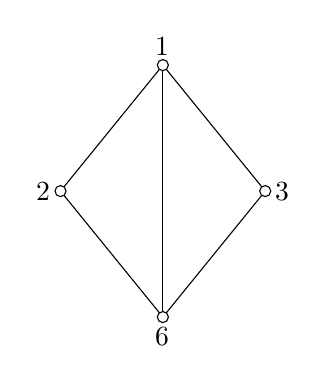
\begin{tikzpicture}
    \coordinate (top) at (0,1.6); \coordinate (left) at (-1.3,0);
    \coordinate (right) at (1.3,0); \coordinate (bot) at (0,-1.6);
    \draw (top) -- (bot); \draw (top) -- (left) -- (bot); \draw (top)
    -- (right) -- (bot); \foreach \p in {top,left,right,bot} {
      \fill[white] (\p) circle (2pt); \draw (\p) circle (2pt); }
    \node[above] at (top) {$1$}; \node[left] at (left) {$2$};
    \node[right] at (right) {$3$}; \node[below] at (bot) {$6$};
  \end{tikzpicture}
  \qquad\qquad
  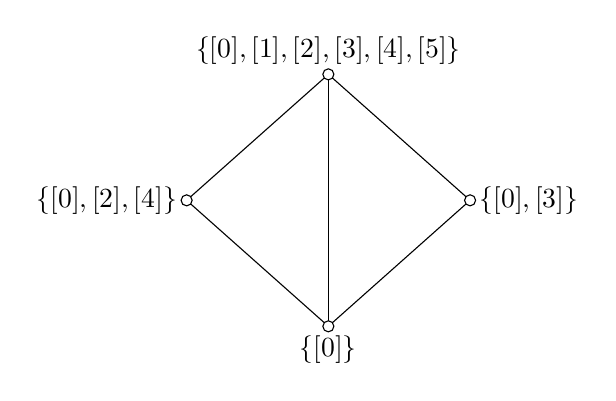
\begin{tikzpicture}
    \coordinate (top) at (0,1.6); \coordinate (left) at (-1.8,0);
    \coordinate (right) at (1.8,0); \coordinate (bot) at (0,-1.6);
    \draw (top) -- (bot); \draw (top) -- (left) -- (bot); \draw (top)
    -- (right) -- (bot); \foreach \p in {top,left,right,bot} {
      \fill[white] (\p) circle (2pt); \draw (\p) circle (2pt); }
    \node[above] at (top) {$\{[0],[1],[2],[3],[4],[5]\}$}; \node[left]
    at (left) {$\{[0],[2],[4]\}$}; \node[right] at (right)
    {$\{[0],[3]\}$}; \node[below] at (bot) {$\{[0]\}$};
  \end{tikzpicture}
\end{center}
where lines connect multiples in one picture and subsets in the other.
The reader will draw the lattice of subgroups of $S_3$, noting that it
looks completely different from the one for $\Z/6\Z$.

Contemplating subgroups of cyclic groups has pretty (and useful)
`number-theoretic' consequences; cf.\ \Cref{exer:groups:euler-totient-sum-formula}.

\subsection{Monomorphisms}
\label{subsec:groups:monomorphisms}
I end this section with some categorical considerations.

If $H$ is a subgroup of $G$, the inclusion $H \hookrightarrow G$ is an
example of a \emph{monomorphism} in $\categ{Grp}$ in the `categorical'
sense of \S{}\ref{subsec:prelims:morphisms:monomorphisms-and-epimorphisms}. In fact, it is easy to characterize all
monomorphisms $\varphi \in \Hom_{\categ{Grp}}(G,G')$ (where $G$, $G'$
are any groups):

\begin{prop}{The following are equivalent:
\begin{enumerate}[label=(\alph*)]
  \item $\varphi$ is a monomorphism;
  \item $\ker\varphi = \{e_G\}$;
  \item $\varphi : G \to G'$ is injective (as a set-function).
  \end{enumerate}}{prop:groups:monomorphism-characterization}
\end{prop}
\begin{proof}
  (a) $\implies$ (b): Assume (a) holds, and consider the two parallel
  compositions
  \[
    \begin{tikzcd}
      \ker\varphi \arrow[r, shift left, "i"] \arrow[r, shift right,
      "e"'] & G \arrow[r, "\varphi"] & G',
    \end{tikzcd}
  \]
  where $i$ is the inclusion and $e$ is the trivial map. Both
  $\varphi \circ i$ and $\varphi \circ e$ are the trivial map; since
  $\varphi$ is a monomorphism, this implies $i = e$. But $i = e$
  implies that $\ker\varphi$ is trivial, that is, (b) holds.

  (b) $\implies$ (c): Assume $\ker\varphi = \{e_G\}$. Then
  \[
    \varphi(g_1) = \varphi(g_2) \implies \varphi(g_1)\varphi(g_2)^{-1}
    = e_{G'} \implies \varphi(g_1 g_2^{-1}) = e_{G'} \implies g_1
    g_2^{-1} \in \ker\varphi \implies g_1 g_2^{-1} = e_G \implies g_1
    = g_2.
  \]
  This shows that $\varphi$ is injective, as needed.

  (c) $\implies$ (a): If $\varphi$ is injective, then it satisfies the
  defining property for monomorphisms in $\categ{Set}$: that is, for
  any set $Z$ and any two set-functions $\alpha', \alpha'' : Z \to G$,
  \[
    \varphi \circ \alpha' = \varphi \circ \alpha'' \iff \alpha' =
    \alpha''.
  \]
  This must hold in particular if $Z$ has a group structure and
  $\alpha'$, $\alpha''$ are group homomorphisms, so $\varphi$ is a
  monomorphism in $\categ{Grp}$.
\end{proof}

The equivalence (a) $\iff$ (c) may lead the reader to think that from
the point of view of monomorphisms, $\categ{Grp}$ and $\categ{Set}$
are pretty much alike. This is not quite so: while it is true that
homomorphisms with a left-inverse are necessarily monomorphisms, as in
$\categ{Set}$ (cf.\ \Cref{exer:groups:left-inverse-implies-monomorphism}), the converse is not true in
$\categ{Grp}$ (cf.\ \Cref{exer:groups:z3z-to-s3-no-left-inverse}).

\subsection*{Exercises}

\begin{exer}{$\lnot$}{exer:groups:matrix-subgroups-inclusions}
  (If you know about matrices.) The group of invertible $n \times n$
  matrices with entries in $\R$ is denoted $\mathrm{GL}_n(\R)$
  (\Cref{exam:groups:gln-matrices}). Similarly, $\mathrm{GL}_n(\C)$ denotes the
  group of $n \times n$ invertible matrices with complex
  entries. Consider the following sets of matrices:
  \begin{itemize}
  \item
    $\mathrm{SL}_n(\R) = \{M \in \mathrm{GL}_n(\R) \mid \det(M) =
    1\}$;
  \item
    $\mathrm{SL}_n(\C) = \{M \in \mathrm{GL}_n(\C)
    \mid \det(M) = 1\}$;
  \item
    $\mathrm{O}_n(\R) = \{M \in \mathrm{GL}_n(\R) \mid MM^t = M^tM =
    I_n\}$;
  \item
    $\mathrm{SO}_n(\R) = \{M \in \mathrm{O}_n(\R) \mid \det(M) = 1\}$;
  \item
    $\mathrm{U}(n) = \{M \in \mathrm{GL}_n(\C) \mid MM^\dagger
    = M^\dagger M = I_n\}$;
  \item $\mathrm{SU}(n) = \{M \in \mathrm{U}(n) \mid \det(M) = 1\}$.
  \end{itemize}
  Here $I_n$ stands for the $n \times n$ identity matrix, $M^t$ is the
  \emph{transpose} of $M$, $M^\dagger$ is the \emph{conjugate
    transpose} of $M$, and $\det(M)$ denotes the
  \emph{determinant}\footnote{If you are not familiar with some of
    these notions, that's ok: leave this exercise and similar ones
    alone if that is the case. We will come back to linear algebra and
    matrices in \Cref{chap:linalg} and following.} of $M$. Find all possible
  inclusions among these sets, and prove that in every case the
  smaller set is a subgroup of the larger one.

  These sets of matrices have compelling geometric interpretations:
  for example, $\mathrm{SO}_3(\R)$ is the group of `rotations' in
  $\R^3$. [\ref{exer:groups:sln-normal-in-gln}, \ref{exer:groups:on-preserves-lengths-angles}, \ref{exer:rings:matrix-ring}, \ref{exer:linalg:6.16}]
\end{exer}
\begin{exer}{$\lnot$}{exer:groups:upper-triangular-subgroup}
  Prove that the set of $2 \times 2$ matrices
  \[
    \begin{pmatrix} a & b \\ 0 & d \end{pmatrix}
  \]
  with $a, b, d$ in $\C$ and $ad \neq 0$ is a subgroup of
  $\mathrm{GL}_2(\C)$. More generally, prove that the set of
  $n \times n$ complex matrices $(a_{ij})_{1 \leq i,j \leq n}$ with
  $a_{ij} = 0$ for $i > j$ and $a_{11} \cdots a_{nn} \neq 0$ is a
  subgroup of $\mathrm{GL}_n(\C)$. (These matrices are called
  `upper triangular', for evident reasons.) [\ref{exer:groups2:gl2c-union-of-conjugates-of-borel}]
\end{exer}
\begin{exer}{$\lnot$}{exer:groups:su2-sphere}
  Prove that every matrix in $\mathrm{SU}(2)$ may be written in the
  form
  \[
    \begin{pmatrix} a+bi & c+di \\ -c+di & a-bi \end{pmatrix}
  \]
  where $a,b,c,d \in \R$ and $a^2+b^2+c^2+d^2=1$. (Thus,
  $\mathrm{SU}(2)$ may be realized as a three-dimensional sphere
  embedded in $\R^4$; in particular, it is simply connected.) [\ref{exer:groups:so3-su2-mod-plusminus-i},
  \ref{exer:rings:quaternion-norm}]
\end{exer}
\begin{exer}{\exerused}{exer:groups:exponential-image-cyclic}
  Let $G$ be a group, and let $g \in G$. Verify that the image of the
  exponential map $\epsilon_g : \Z \to G$ is a cyclic group (in the
  sense of \Cref{defn:groups:cyclic}). [\S{}\ref{subsec:groups:example-subgroup-generated-by-a-subset}, \S{}\ref{subsec:groups:example}]
\end{exer}
\begin{exer}{}{exer:groups:nth-powers-subgroup-commutative}
  Let $G$ be a commutative group, and let $n > 0$ be an integer. Prove
  that $\{g^n \mid g \in G\}$ is a subgroup of $G$. Prove that this is
  not necessarily the case if $G$ is not commutative.
\end{exer}
\begin{exer}{}{exer:groups:union-of-subgroups}
  Prove that the union of a family of subgroups of a group $G$ is not
  necessarily a subgroup of $G$. In fact:
  \begin{itemize}
  \item Let $H$, $H'$ be subgroups of a group $G$. Prove that
    $H \cup H'$ is a subgroup of $G$ only if $H \subseteq H'$ or
    $H' \subseteq H$.
  \item On the other hand, let
    $H_0 \subseteq H_1 \subseteq H_2 \subseteq \dots$ be subgroups of
    a group $G$. Prove that $\bigcup_{i \geq 0} H_i$ is a subgroup of
    $G$.
  \end{itemize}
\end{exer}
\begin{exer}{$\lnot$}{exer:groups:inn-cyclic-iff-abelian}
  Show that \emph{inner automorphisms} (cf.\ \Cref{exer:groups:inner-automorphisms}) form a
  subgroup of $\Aut(G)$; this subgroup is denoted
  $\operatorname{Inn}(G)$. Prove that $\operatorname{Inn}(G)$ is
  cyclic if and only if $\operatorname{Inn}(G)$ is trivial if and only
  if $G$ is abelian. (Hint: Assume that $\operatorname{Inn}(G)$ is
  cyclic; with notation as in \Cref{exer:groups:inner-automorphisms}, this means that there
  exists an element $a \in G$ such that
  $\forall g \in G\ \exists n \in \Z\ \gamma_g = \gamma_a^n$. In
  particular, $gag^{-1} = a^naa^{-n} = a$. Thus $a$ commutes with
  every $g$ in $G$. Therefore\dots.) Deduce that if
  $\Aut(G)$ is cyclic, then $G$ is abelian. [\ref{exer:groups:normal-iff-inn-stabilizes},
  \ref{exer:groups2:quot-ctr-iso-inn}]
\end{exer}
\begin{exer}{}{exer:groups:finitely-generated-abelian-surjection}
  Prove that an \emph{abelian} group $G$ is finitely generated if and
  only if there is a surjective homomorphism
  \[
    \underbrace{\Z \oplus \cdots \oplus \Z}_{n\text{ times}}
    \twoheadrightarrow G
  \]
  for some $n$.
\end{exer}
\begin{exer}{}{exer:groups:q-finitely-generated-subgroups-cyclic}
  Prove that every finitely generated subgroup of $\Q$ is cyclic.
  Prove that $\Q$ is not finitely generated.
\end{exer}
\begin{exer}{$\lnot$}{exer:groups:sl2z-generated-by-s-t}
  The set of $2 \times 2$ matrices with integer entries and
  determinant $1$ is denoted $\mathrm{SL}_2(\Z)$:
  \[
    \mathrm{SL}_2(\Z) = \left\{ \begin{pmatrix} a & b \\ c &
        d \end{pmatrix} \text{ such that } a,b,c,d \in \Z,\ ad-bc=1
    \right\}.
  \]
  Prove that $\mathrm{SL}_2(\Z)$ is generated by the matrices
  \[
    s = \begin{pmatrix} 0 & -1 \\ 1 & 0 \end{pmatrix} \quad \text{and}
    \quad t = \begin{pmatrix} 1 & 1 \\ 0 & 1 \end{pmatrix}.
  \]
  (Hint: This is a little tricky. Let $H$ be the subgroup generated by
  $s$ and $t$. Given a matrix
  $m = \begin{pmatrix} a & b \\ c & d \end{pmatrix}$ in
  $\mathrm{SL}_2(\Z)$, it suffices to show that you can obtain the
  identity by multiplying $m$ by suitably chosen elements of $H$.
  Prove that $\begin{pmatrix} 1 & -q \\ 0 & 1 \end{pmatrix}$ and
  $\begin{pmatrix} 1 & 0 \\ -q & 1 \end{pmatrix}$ are in $H$, and note
  that
  \[
    \begin{pmatrix} a & b \\ c & d \end{pmatrix}
    \begin{pmatrix} 1 & -q \\ 0 & 1 \end{pmatrix} = \begin{pmatrix} a
      & b-qa \\ c & d-qc \end{pmatrix} \quad \text{and} \quad
    \begin{pmatrix} a & b \\ c & d \end{pmatrix}
    \begin{pmatrix} 1 & 0 \\ -q & 1 \end{pmatrix} = \begin{pmatrix}
      a-qb & b \\ c-qd & d \end{pmatrix}.
  \]
  Note that if $c$ and $d$ are both nonzero, one of these two
  operations may be used to decrease the absolute value of one of
  them. Argue that suitable applications of these operations reduce to
  the case in which $c=0$ or $d=0$. Prove directly that $m \in H$ in
  that case.) [\ref{exer:groups:psl2z-modular-group}]
\end{exer}
\begin{exer}{}{exer:groups:s3-not-coproduct-of-cyclic}
  Since direct sums are coproducts in $\categ{Ab}$, the classification
  theorem for abelian groups mentioned in the text says that every
  finitely generated abelian group is a coproduct of cyclic groups in
  $\categ{Ab}$. The reader may be tempted to conjecture that every
  finitely generated group is a coproduct in $\categ{Grp}$. Show that
  this is not the case, by proving that $S_3$ is not a coproduct of
  cyclic groups.
\end{exer}
\begin{exer}{}{exer:groups:mn-generated-subgroup-of-z}
  Let $m$, $n$ be positive integers, and consider the subgroup
  $\langle m,n \rangle$ of $\Z$ they generate. By \Cref{prop:groups:subgroups-of-z},
  \[
    \langle m,n \rangle = d\Z
  \]
  for some positive integer $d$. What is $d$, in relation to $m$, $n$?
\end{exer}
\begin{exer}{$\lnot$}{exer:groups:lattices-c2c2-c4-s3-c6}
  Draw and compare the lattices of subgroups of $C_2 \times C_2$ and
  $C_4$. Draw the lattice of subgroups of $S_3$, and compare it with
  the one for $C_6$. [\ref{exer:groups:s3-normal-subgroups}]
\end{exer}
\begin{exer}{\exerused}{exer:groups:euler-totient-sum-formula}
  If $m$ is a positive integer, denote by $\varphi(m)$ the number of
  positive integers $r \leq m$ that are relatively prime to $m$ (that
  is, for which the gcd of $r$ and $m$ is $1$); this is called Euler's
  $\varphi$- (or `totient') function. For example, $\varphi(12) =
  4$. In other words, $\varphi(m)$ is the order of the group
  $(\Z/m\Z)^*$; cf.\ \Cref{prop:groups:units-group}.

  Put together the following observations:
  \begin{itemize}
  \item $\varphi(m) = $ the number of generators of $C_m$,
  \item every element of $C_n$ generates a subgroup of $C_n$,
  \item the discussion following \Cref{prop:groups:subgroups-of-znz} (in particular,
    every subgroup of $C_n$ is isomorphic to $C_m$, for some
    $m \mid n$),
  \end{itemize}
  to obtain a proof of the formula
  \[
    \sum_{m>0,\, m\mid n} \varphi(m) = n.
  \]
  (For example,
  $\varphi(1)+\varphi(2)+\varphi(3)+\varphi(4)+\varphi(6)+\varphi(12)
  = 1+1+2+2+2+4 = 12$.) [\ref{exer:groups:aut-cn-euler-phi}, $\S$\ref{subsec:groups:example-subgroups-of-cyclic-groups}, \ref{exer:groups:n-divides-phi-an-minus-1}, \ref{exer:irred:crt-znz-decomp-and-totient-formula}, $\S$\ref{subsec:fields:cyclotomic-polynomials-and-fields}]
\end{exer}
\begin{exer}{\exerused}{exer:groups:left-inverse-implies-monomorphism}
  Prove that if a group homomorphism $\varphi : G \to G'$ has a
  left-inverse, that is, a group homomorphism $\psi : G' \to G$ such
  that $\psi \circ \varphi = \id_G$, then $\varphi$ is a
  monomorphism.  [\S{}\ref{subsec:groups:monomorphisms}, \ref{exer:groups:z3z-to-s3-no-left-inverse}]
\end{exer}
\begin{exer}{\exerused}{exer:groups:z3z-to-s3-no-left-inverse}
  Counterpoint to \Cref{exer:groups:left-inverse-implies-monomorphism}: the homomorphism
  $\varphi : \Z/3\Z \to S_3$ given by
  \[
    \varphi([0]) = \begin{pmatrix}1&2&3\\1&2&3\end{pmatrix}, \quad
    \varphi([1]) = \begin{pmatrix}1&2&3\\3&1&2\end{pmatrix}, \quad
    \varphi([2]) = \begin{pmatrix}1&2&3\\2&3&1\end{pmatrix}
  \]
  is a monomorphism; show that it has no left-inverse in
  $\categ{Grp}$.  (Knowing about normal subgroups will make this
  problem particularly easy.) [\S{}\ref{subsec:groups:monomorphisms}]
\end{exer}

\section{Quotient groups}
\label{sec:groups:quotient-groups}


\subsection{Normal subgroups}
\label{subsec:groups:normal-subgroups}
Before tackling `quotient groups', I should clarify in what sense
kernels are \emph{special} subgroups, as claimed in \S{}\ref{subsec:groups:examples-kernel-and-image}.

\begin{defn}{Normal subgroup}{defn:groups:normal-subgroup}
  A subgroup $N$ of a group $G$ is \emph{normal} if $\forall g \in G$,
  $\forall n \in N$,
  \[
    gng^{-1} \in N.
  \]
\end{defn}

Note that \emph{every} subgroup of a commutative group is normal
(because then $\forall g \in G$, $gng^{-1} = n \in N$). However, in
general \emph{not all} subgroups are normal: examples may be found
already in $S_3$ (cf.\ \Cref{exer:groups:s3-normal-subgroups}). There exist noncommutative
groups in which every subgroup is normal (one example is the
`quaternionic group' $Q_8$; cf.\ \Cref{exer:rings:quaternions} (iv)), but they are
very rare.

\begin{lem}{If $\varphi : G \to G'$ is any group homomorphism, then
    $\ker\varphi$ is a normal subgroup of
    $G$.}{lem:groups:kernel-is-normal}
\end{lem}
\begin{proof}
  We already know that $\ker\varphi$ is a subgroup of $G$; to verify
  it is normal note that $\forall g \in G$,
  $\forall n \in \ker\varphi$
  \[
    \varphi(gng^{-1}) = \varphi(g)\varphi(n)\varphi(g^{-1}) =
    \varphi(g)e_{G'}\varphi(g)^{-1} = e_{G'},
  \]
  proving that $gng^{-1} \in \ker\varphi$.
\end{proof}

Loosely speaking, therefore, \emph{kernel $\implies$ normal}. In fact
more is true, as we will see in a little while; for now I don't want
to spoil the surprise for the reader. (Can the reader guess?)

There is a convenient shorthand to express conditions such as
normality: if $g \in G$ and $A \subseteq G$ is any subset, we denote
by $gA$, $Ag$, respectively, the following subsets of $G$:
\[
  gA := \{h \in G \mid (\exists a \in A) : h = ga\}, \qquad Ag := \{h
  \in G \mid (\exists a \in A) : h = ag\}.
\]
Then the normality condition can be expressed by
\[
  (\forall g \in G) : \quad gNg^{-1} \subseteq N,
\]
or in a number of other ways:
\[
  gNg^{-1} = N \quad \text{or} \quad gN \subseteq Ng \quad \text{or}
  \quad gN = Ng
\]
for all $g \in G$. The reader should check that these are indeed
equivalent conditions (\Cref{exer:groups:normality-conditions-equivalent}) and keep in mind that `$gN = Ng$'
does \emph{not} mean that $g$ commutes with every element of $N$; it
means that if $n \in N$, then there are elements $n', n'' \in N$, in
general different from $n$, such that $gn = n'g$ (so that
$gN \subseteq Ng$) and $ng = gn''$ (so that $Ng \subseteq gN$).

\subsection{Quotient group}
\label{subsec:groups:quotient-group}
Recall that we have the notion of a quotient of a \emph{set} by an
equivalence relation (\S{}\ref{subsec:prelims:equiv-relations}) and that this notion satisfies a
universal property (clumsily stated in \S{}\ref{subsec:prelims:quotients}). It is natural to
investigate this notion in $\categ{Grp}$.

We consider then an equivalence relation $\sim$ on (the set
underlying) a group $G$; we seek a group $G/\!\sim$ and a group
homomorphism $\pi : G \to G/\!\sim$ satisfying the appropriate
universal property, that is, initial with respect to group
homomorphisms $\varphi : G \to G'$ such that
$a \sim b \implies \varphi(a) = \varphi(b)$.

It is natural to try to construct the group $G/\!\sim$ by defining an
operation $\bullet$ on the \emph{set} $G/\!\sim$. The situation is
tightly constrained by the requirement that the quotient map
$\pi : G \to G/\!\sim$ (as in \S{}\ref{subsec:prelims:functions:monomorphisms-and-epimorphisms}) be a group homomorphism: for
if $[a] = \pi(a)$, $[b] = \pi(b)$ are elements of $G/\!\sim$ (that is,
equivalence classes with respect to $\sim$), then the homomorphism
condition \emph{forces}
\[ [a] \bullet [b] = \pi(a) \bullet \pi(b) = \pi(ab) = [ab].
\]
But is this operation well-defined? This amounts to conditions on the
equivalence relation, which we proceed to unearth.

For the operation to be well-defined `in the first factor', it is
necessary that if $[a] = [a']$, then $[ab] = [a'b]$ regardless of what
$b$ is; that is,
\[
  (\forall g \in G) : \quad a \sim a' \implies ag \sim a'g.
\]
Similarly, for the operation to be well-defined in the second factor
we need
\[
  (\forall g \in G) : \quad a \sim a' \implies ga \sim ga'.
\]
Luckily, this is all that there is to it:

\begin{prop}{With notation as above, the operation
    \[ [a] \bullet [b] := [ab]
\]
defines a group structure on $G/\!\sim$ if and only if
$\forall a, a', g \in G$
\[
  a \sim a' \implies ga \sim ga' \text{ and } ag \sim a'g.
\]
In this case the quotient function $\pi : G \to G/\!\sim$ is a
homomorphism and is universal with respect to homomorphisms
$\varphi : G \to G'$ such that
$a \sim a' \implies \varphi(a) =
\varphi(a')$.}{prop:groups:quotient-group-universal-property}
\end{prop}
\begin{proof}
  We have already noted that the condition is necessary. To prove it
  is sufficient, with the stated consequences, assume
  $\forall a, a', g \in G$
  \[
    a \sim a' \implies ga \sim ga' \text{ and } ag \sim a'g.
  \]
  Then the operation
  \[ [a] \bullet [b] := [ab]
  \]
  is well-defined, and we have to verify that it defines a group
  structure on $G/\!\sim$. The associativity of $\bullet$ is inherited
  from the associativity of $G$: $\forall a,b,c \in G$
  \[
    ([a] \bullet [b]) \bullet [c] = [ab] \bullet [c] = [(ab)c] =
    [a(bc)] = [a] \bullet [bc] = [a] \bullet ([b] \bullet [c]).
  \]
  The class $[e_G]$ is an identity with respect to this operation:
  $\forall g \in G$
  \[ [g] \bullet [e_G] = [ge_G] = [g], \qquad [e_G] \bullet [g] =
    [e_Gg] = [g].
  \]
  The class $[g^{-1}]$ is the inverse of $[g]$:
  \[ [g^{-1}] \bullet [g] = [g^{-1}g] = [e_G], \qquad [g] \bullet
    [g^{-1}] = [gg^{-1}] = [e_G].
  \]
  This shows $G/\!\sim$ is indeed a group, and we have already
  observed that $\pi : G \to G/\!\sim$ is a homomorphism: this is what
  led us to the definition of $\bullet$.

  To prove that $G/\!\sim$ satisfies the universal property, assume
  \[
    \varphi : G \to G'
  \]
  is a group homomorphism such that
  $a \sim a' \implies \varphi(a) = \varphi(a')$. Since (cf.\
  \S{}\ref{subsec:prelims:quotients}) the \emph{set} $G/\!\sim$ satisfies the corresponding
  universal property in $\categ{Set}$, we know that there exists a
  unique set-function
  \[
    \bar\varphi : G/\!\sim \to G',
  \]
  defined\footnote{The point of \S{}\ref{subsec:prelims:quotients} is precisely that this
    function is well-defined.} by $\bar\varphi([a]) := \varphi(a)$. So
  we only need to check that this function $\bar\varphi$ is in fact a
  group homomorphism, and this is immediate:
  \[
    \bar\varphi([a] \bullet [b]) = \bar\varphi([ab]) = \varphi(ab) =
    \varphi(a)\varphi(b) = \bar\varphi([a])\bar\varphi([b])
  \]
  for all $[a], [b] \in G/\!\sim$, as needed.
\end{proof}

I will say that $\sim$ is \emph{compatible} with the group structure
of $G$ if the condition given in
Proposition~\ref{prop:groups:quotient-group-universal-property} holds.
Since the operation $\bullet$ on the quotient $G/\!\sim$ is uniquely
determined by the operation on $G$, I yield to the usual abuse of
language and omit it. If $\sim$ is compatible, I will call $G/\!\sim$
the \emph{quotient group} of $G$ by $\sim$.

\subsection{Cosets}
\label{subsec:groups:cosets}
The conditions obtained in
Proposition~\ref{prop:groups:quotient-group-universal-property},
\begin{align}
  \tag{$\dagger$} (\forall g \in G) &: \quad a \sim b \implies ga \sim gb, \\
  \tag{$\dagger\dagger$} (\forall g \in G) &: \quad a \sim b \implies ag \sim bg,
\end{align}
lead to a complete description of \emph{all} compatible relations on a
group $G$. In fact, each of these two conditions leads to a
description of the relations satisfying it, and we will analyze them
separately; the reader should keep in mind that we have a group
structure on $G/\!\sim$ only if \emph{both} are satisfied.

Let's begin with $(\dagger)$. Here is the description:

\begin{prop}{Let $\sim$ be an equivalence relation on a group $G$,
satisfying $(\dagger)$. Then
\begin{itemize}
\item the equivalence class of $e_G$ is a subgroup $H$ of $G$; and
\item $a \sim b \iff a^{-1}b \in H \iff aH = bH$.
\end{itemize}}{prop:groups:coset-description-dagger}
\end{prop}
\begin{proof}
  Let $H \subseteq G$ be the equivalence class of the identity;
  $H \neq \emptyset$ as $e_G \in H$. For $a, b \in H$, we have
  $e_G \sim b$ and hence $b^{-1} \sim e_G$ (applying $(\dagger)$,
  multiplying on the left by $b^{-1}$); hence $ab^{-1} \sim a$ (by
  $(\dagger)$ again, multiplying on the left by $a$); and hence
  \[
    ab^{-1} \sim a \sim e_G
  \]
  by the transitivity of $\sim$ and since $a \in H$. This shows that
  $ab^{-1} \in H$ for all $a, b \in H$, proving that $H$ is a subgroup
  (by Proposition~\ref{prop:groups:subgroup-criterion}).

  Next, assume $a, b \in G$ and $a \sim b$. Multiplying on the left by
  $a^{-1}$, $(\dagger)$ implies $e_G \sim a^{-1}b$, that is,
  $a^{-1}b \in H$. Since $H$ is closed under the operation, this
  implies $a^{-1}bH \subseteq H$, hence $bH \subseteq aH$; as $\sim$
  is symmetric, the same reasoning gives $aH \subseteq bH$; and hence
  $aH = bH$. Thus, we have proved
  \[
    a \sim b \implies a^{-1}b \in H \implies aH = bH.
  \]
  Finally, assume $aH = bH$. Then $a = ae_G \in bH$, and hence
  $a^{-1}b \in H$. By definition of $H$, this means
  $e_G \sim a^{-1}b$.  Multiplying on the left by $a$ shows (by
  $(\dagger)$ again) that $a \sim b$, completing the proof.
\end{proof}

Proposition~\ref{prop:groups:coset-description-dagger} shows that the
equivalence classes of an equivalence relation satisfying $(\dagger)$
are in fact all of the form
\[
  aH
\]
for a fixed subgroup $H$, as $a$ ranges in $G$. These important
subsets determined by a subgroup $H$ deserve a name.

\begin{defn}{Left-/right-cosets}{defn:groups:cosets}
  The \emph{left-cosets} of a subgroup $H$ in a group $G$ are the sets
  $aH$, for $a \in G$. The \emph{right-cosets} of $H$ are the sets
  $Ha$, $a \in G$.
\end{defn}

Now, a `converse' to
Proposition~\ref{prop:groups:coset-description-dagger} holds:

\begin{prop}{If $H$ is any subgroup of a group $G$, the relation
$\sim_L$ defined by
\[
  (\forall a, b \in G) : \quad a \sim_L b \iff a^{-1}b \in H
\]
is an equivalence relation satisfying
$(\dagger)$.}{prop:groups:sim-l-satisfies-dagger}
\end{prop}
\begin{proof}
  This is straightforward and is mostly left to the reader
  (\Cref{exer:groups:prove-prop-7-6}). To see that the relation satisfies $(\dagger)$, note
  that
  \[
    a \sim_L b \implies a^{-1}b \in H \implies a^{-1}(g^{-1}g)b \in H
    \implies (ga)^{-1}(gb) \in H \implies ga \sim_L gb
  \]
  for all $g \in G$.
\end{proof}

Taken together,
Propositions~\ref{prop:groups:coset-description-dagger}
and~\ref{prop:groups:sim-l-satisfies-dagger} show

\begin{prop}{There is a one-to-one correspondence between subgroups of
    $G$ and equivalence relations on $G$ satisfying $(\dagger)$; for
    the relation $\sim_L$ corresponding to a subgroup $H$,
    $G/\!\sim_L$ may be described as the set of left-cosets $aH$ of
    $H$.}{prop:groups:subgroups-correspond-to-dagger-relations}
\end{prop}

The reader should have no difficulty producing the mirror statements
(and proofs) giving a similarly exhaustive description of all
equivalence relations satisfying $(\dagger\dagger)$. The end result
will be

\begin{prop}{There is a one-to-one correspondence between subgroups of
    $G$ and equivalence relations on $G$ satisfying
    $(\dagger\dagger)$; for the relation $\sim_R$ corresponding to a
    subgroup $H$, $G/\!\sim_R$ may be described as the set of
    right-cosets $Ha$ of
    $H$.}{prop:groups:subgroups-correspond-to-daggerdagger-relations}
\end{prop}
The relation corresponding to $H$ in this second way is defined by
\[
  a \sim_R b \iff ab^{-1} \in H \iff Ha = Hb.
\]

What may be surprising at first is that the relations $\sim_L$ and
$\sim_R$ corresponding to the \emph{same} subgroup $H$ may very well
not be the same relation. That is, left-cosets and right-cosets of a
subgroup need not coincide. Of course $eH = He = H$, and more
generally
\[
  (\forall h \in H) : \quad hH = Hh = H.
\]
Further
\[
  (\forall a \in G) : \quad a \in aH \cap Ha;
\]
hence, if $aH = Hb$ for any $b$, then in fact necessarily $aH = Ha$.
This is of course automatically true if $G$ is commutative, but it is
simply not the case in general.

\begin{exam}{}{exam:groups:s3-left-right-cosets}
  Let $G = S_3$, and let $H$ be the subgroup consisting of the
  identity and the $1 \leftrightarrow 2$ switch:
  \[
    H = \left\{ \begin{pmatrix}1&2&3\\1&2&3\end{pmatrix},
      \begin{pmatrix}1&2&3\\2&1&3\end{pmatrix} \right\}.
  \]
  Then
  \[
    \begin{pmatrix}1&2&3\\3&1&2\end{pmatrix} H =
    \left\{ \begin{pmatrix}1&2&3\\3&1&2\end{pmatrix},
      \begin{pmatrix}1&2&3\\3&2&1\end{pmatrix} \right\},
  \]
  while
  \[
    H \begin{pmatrix}1&2&3\\3&1&2\end{pmatrix} =
    \left\{ \begin{pmatrix}1&2&3\\3&1&2\end{pmatrix},
      \begin{pmatrix}1&2&3\\1&3&2\end{pmatrix} \right\}.
  \]
  This state of affairs simply reflects the fact that the two
  conditions $(\dagger)$ and $(\dagger\dagger)$ are different: there
  is no reason to expect that if one holds, the other one should also
  hold (unless $G$ is commutative, of course). Once more, keep in mind
  that \emph{both} have to hold for the quotient $G/\!\sim$ to be a
  group, compatibly with the operation in $G$; cf.\
  Proposition~\ref{prop:groups:quotient-group-universal-property}.
\end{exam}

\subsection{Quotient by normal subgroups}
\label{subsec:groups:quotient-by-normal-subgroups}
To stress the main point again, an arbitrary subgroup $H$ of $G$ leads
to two partitions of $G$, which we have denoted
\[
  G/\!\sim_L\, = \{aH \mid a \in G\}, \qquad G/\!\sim_R\, = \{Ha \mid
  a \in G\}.
\]
The relation $\sim_L$ satisfies property $(\dagger)$ listed at the
beginning of \S{}\ref{subsec:groups:cosets}; $\sim_R$ satisfies $(\dagger\dagger)$. A priori,
these relations, and hence the corresponding partitions, are
different.

The condition that $\sim_L$ and $\sim_R$ coincide (as is necessarily
the case, for example, if $G$ is commutative) translates into a
condition on $H$: for such `special' subgroups, $(\dagger)$ and
$(\dagger\dagger)$ get back together. The good news is that this
condition is easy to identify and is not new to the reader.

\begin{prop}{The relations $\sim_L$, $\sim_R$ corresponding to a
    subgroup $H$ coincide if and only if $H$ is
    normal.}{prop:groups:sim-l-sim-r-coincide-iff-normal}
\end{prop}
\begin{proof}
  Two relations coincide if the corresponding partitions agree.
  Therefore
  \[
    \sim_L\, = \sim_R \iff \text{left- and right-cosets of } H \text{
      coincide} \iff (\forall g \in G) : gH = Hg.
  \]
  But this is one of the equivalent conditions defining the notion of
  normal subgroup (cf.\ \S{}\ref{subsec:groups:normal-subgroups}), proving the statement.
\end{proof}

The innocent-looking
Proposition~\ref{prop:groups:sim-l-sim-r-coincide-iff-normal} is of
fundamental importance. If $H$ is normal, then the one equivalence
relation $\sim\, = \sim_L\, = \sim_R$ corresponding to $H$ satisfies
both $(\dagger)$ and $(\dagger\dagger)$ (by
Proposition~\ref{prop:groups:coset-description-dagger} and its mirror
statement), and hence (by
Proposition~\ref{prop:groups:quotient-group-universal-property}) the
quotient
\[
  G/\!\sim\, = \{aH \mid a \in G\} = \{Ha \mid a \in G\}
\]
has a natural group structure.

\begin{defn}{Quotient group of $G$ modulo $H$}{defn:groups:quotient-group-modulo-h}
  Let $H$ be a normal subgroup of a group $G$. The \emph{quotient
    group of $G$ modulo $H$}, denoted\footnote{In a large display I
    sometime use the full `fraction' notation $\frac{G}{H}$.} $G/H$,
  is the group $G/\!\sim$ obtained from the relation $\sim$ defined
  above. In terms of (left-)cosets, the product in $G/H$ is defined by
  \[
    (aH)(bH) := (ab)H.
  \]
  The identity element $e_{G/H}$ of the quotient group $G/H$ is the
  coset of the identity, $e_GH = H$.
\end{defn}

By Proposition~\ref{prop:groups:quotient-group-universal-property},
the quotient function
\[
  \pi : G \to G/H
\]
sending $g \in G$ to $gH = Hg$ is a group homomorphism and is
universal with respect to group homomorphisms $\varphi : G \to G'$
such that $aH = bH \implies \varphi(a) = \varphi(b)$. This universal
property is extremely useful, so I will grace it with theorem status:

\begin{thm}{Let $H$ be a normal subgroup of a group $G$. Then for
    every group homomorphism $\varphi : G \to G'$ such that
    $H \subseteq \ker\varphi$ there exists a unique group homomorphism
    $\bar\varphi : G/H \to G'$ so that the diagram
    commutes.}{thm:groups:quotient-universal-property}
  \[
    \begin{tikzcd}
      G \arrow[r, "\varphi"] \arrow[d, "\pi"'] & G' \\
      G/H \arrow[ur, dashed, "\exists ! \bar\varphi"'] &
    \end{tikzcd}
  \]
\end{thm}
\begin{proof}
  We only need to match the stated universal property with the one we
  proved in
  Proposition~\ref{prop:groups:quotient-group-universal-property}, and
  indeed,
  \[
    H \subseteq \ker\varphi \iff (\forall h \in H) : \varphi(h) =
    e_{G'}
  \]
  is equivalent to
  \[
    (\forall a, b \in G) : ab^{-1} \in H \implies \varphi(ab^{-1}) =
    e_{G'}
  \]
  that is, to
  \[
    (\forall a, b \in G) : ab^{-1} \in H \implies \varphi(a) =
    \varphi(b)
  \]
  and finally, keeping in mind how the relation $\sim$ corresponding
  to $H$ is defined,
  \[
    (\forall a, b \in G) : a \sim b \implies \varphi(a) = \varphi(b),
  \]
  the condition giving the universal property in
  Proposition~\ref{prop:groups:quotient-group-universal-property}.
\end{proof}

\subsection{Example}
\label{subsec:groups:example}
The reader is already very familiar with an important class of
examples: the cyclic groups $\Z/n\Z$. Indeed, in \S{}\ref{subsec:groups:cyclic-groups-and-modular-arithmetic} we defined
$\Z/n\Z$ as the set of equivalence classes in $\Z$ with respect to the
congruence equivalence relation
\[
  (\forall a, b \in \Z) : \quad a \equiv b \mod n \iff n \mid (b-a).
\]
Now we recognize that $n \mid (b-a)$ is equivalent to
\[
  b - a \in n\Z,
\]
which is the relation $\sim_L$ corresponding (in `abelian' notation)
to the subgroup $n\Z$ of $\Z$. This subgroup is of course normal,
since $\Z$ is abelian. The `congruence classes mod $n$' are nothing
but the cosets of the subgroup $n\Z$ in $\Z$; using abelian notation
for cosets, we could write
\[ [a]_n = a + (n\Z).
\]
Of course the operation defined on $\Z/n\Z$ in \S{}\ref{subsec:groups:cyclic-groups-and-modular-arithmetic} matches
precisely the one defined above for quotient groups. This justifies
the notation $\Z/n\Z$ introduced in \S{}\ref{subsec:groups:cyclic-groups-and-modular-arithmetic}.

The reader can already appreciate in this simple context the
usefulness of
Theorem~\ref{thm:groups:quotient-universal-property}. Let $g \in G$ be
an element of order $n$ and consider the exponential map
\[
  \epsilon_g : \Z \to G, \quad N \mapsto g^N.
\]
By Corollary~\ref{coro:groups:order-multiple},
\[
  \ker\epsilon_g = \{N \in \Z \mid N \text{ is a multiple of } |g|\} =
  n\Z.
\]
Theorem~\ref{thm:groups:quotient-universal-property} then implies
right away that $\epsilon_g$ factors through the quotient:
\[
  \begin{tikzcd}
    \Z \arrow[r, "\epsilon_g"] \arrow[d, "\pi_n"'] & G \\
    \Z/n\Z \arrow[ur, dashed, "\exists ! \bar\epsilon_g"'] &
  \end{tikzcd}
\]
That is, there is an induced map
\[
  \Z/n\Z \to \langle g \rangle.
\]
In fact, the `canonical decomposition' of \S{}\ref{subsec:prelims:canonical-decomposition} implies that this
is an isomorphism (verifying that $\langle g \rangle$ is cyclic in the
sense of \Cref{defn:groups:cyclic}, as the reader should have checked `by hand'
already in \Cref{exer:groups:exponential-image-cyclic}). We will formalize this observation in
general in the next section.

Also note that $|g| = n = |\langle g \rangle|$ in this case.

\subsection{\texorpdfstring{kernel $\Leftrightarrow$ normal}{kernel
    iff normal}}
\label{subsec:groups:kernel-iff-normal}
If $H$ is a normal subgroup, we have now constructed in gory detail a
group $G/H$ and a surjective homomorphism
\[
  \pi : G \to G/H.
\]
What is the kernel of $\pi$? The identity of $G/H$ is the coset
$e_GH$, that is, $H$ itself. Therefore
\[
  \ker\pi = \{g \in G \mid gH = H\} = H.
\]
This observation completes the circle of ideas begun in \S{}\ref{subsec:groups:normal-subgroups}: there
we had noticed that every kernel (of a group homomorphism) is a normal
subgroup; and now we have verified that every normal subgroup is in
fact a \emph{kernel} (of some group homomorphism). I encapsulate this
in the slogan
\[
  \text{kernel} \iff \text{normal}:
\]
in group theory\footnote{We will run into analogous observations in
  ring theory, where we will verify that kernels and \emph{ideals}
  coincide, and for modules, as kernels and \emph{submodules} again
  coincide.}, `kernel' and `normal subgroup' are equivalent concepts.

For example, every subgroup in an abelian group is the kernel of some
homomorphism: yet another indication that life is simpler in
$\categ{Ab}$ than in $\categ{Grp}$.

\subsection*{Exercises}

\begin{exer}{\exerused}{exer:groups:s3-normal-subgroups}
  List all subgroups of $S_3$ (cf.\ \Cref{exer:groups:lattices-c2c2-c4-s3-c6}) and determine which
  subgroups are normal and which are not normal. [\S{}\ref{subsec:groups:normal-subgroups}]
\end{exer}
\begin{exer}{}{exer:groups:image-not-necessarily-normal}
  Is the \emph{image} of a group homomorphism necessarily a normal
  subgroup of the target?
\end{exer}
\begin{exer}{\exerused}{exer:groups:normality-conditions-equivalent}
  Verify that the equivalent conditions for normality given in \S{}\ref{subsec:groups:normal-subgroups}
  are indeed equivalent. [\S{}\ref{subsec:groups:normal-subgroups}]
\end{exer}
\begin{exer}{}{exer:groups:exercise-5-10-relation-compatible}
  Prove that the relation defined in \Cref{exer:groups:fab-quotient-by-2g} on a free abelian
  group $F = F^{ab}(A)$ is compatible with the group
  structure. Determine the quotient $F/\!\sim$ as a better known
  group.
\end{exer}
\begin{exer}{$\lnot$}{exer:groups:psl2z-modular-group}
  Define an equivalence relation $\sim$ on $\mathrm{SL}_2(\Z)$ by
  letting $A \sim A' \iff A' = \pm A$. Prove that $\sim$ is compatible
  with the group structure. The quotient $\mathrm{SL}_2(\Z)/\!\sim$ is
  denoted $\mathrm{PSL}_2(\Z)$ and is called the \emph{modular group};
  it would be a serious contender in a contest for `the most important
  group in mathematics', due to its role in algebraic geometry and
  number theory. Prove that $\mathrm{PSL}_2(\Z)$ is generated by the
  (cosets of the) matrices
  \[
    \begin{pmatrix} 0 & -1 \\ 1 & 0 \end{pmatrix} \quad \text{and}
    \quad
    \begin{pmatrix} 1 & -1 \\ 1 & 0 \end{pmatrix}.
  \]
  (You will not need to work very hard, if you use the result of
  \Cref{exer:groups:sl2z-generated-by-s-t}.) Note that the first has order $2$ in
  $\mathrm{PSL}_2(\Z)$, the second has order $3$, and their product
  has infinite order. [\ref{exer:groups:psl2z-coproduct-c2-c3}]
\end{exer}
\begin{exer}{}{exer:groups:gn-relation-equivalence-commutative}
  Let $G$ be a group, and let $n$ be a positive integer. Consider the
  relation
  \[
    a \sim b \iff (\exists g \in G)\ ab^{-1} = g^n.
  \]
  \begin{itemize}
  \item Show that in general $\sim$ is \emph{not} an equivalence
    relation.
  \item Prove that $\sim$ is an equivalence relation if $G$ is
    commutative, and determine the corresponding subgroup of $G$.
  \end{itemize}
\end{exer}
\begin{exer}{}{exer:groups:order-n-elements-generate-normal}
  Let $G$ be a group, $n$ a positive integer, and let $H \subseteq G$
  be the subgroup generated by all elements of order $n$ in $G$. Prove
  that $H$ is normal.
\end{exer}
\begin{exer}{\exerused}{exer:groups:prove-prop-7-6}
  Prove
  Proposition~\ref{prop:groups:sim-l-satisfies-dagger}. [\S{}\ref{subsec:groups:cosets}]
\end{exer}
\begin{exer}{}{exer:groups:mirror-statements-daggerdagger}
  State and prove the `mirror' statements of
  Propositions~\ref{prop:groups:coset-description-dagger}
  and~\ref{prop:groups:sim-l-satisfies-dagger}, leading to the
  description of relations satisfying $(\dagger\dagger)$.
\end{exer}
\begin{exer}{$\lnot$}{exer:groups:normal-iff-inn-stabilizes}
  Let $G$ be a group, and $H \subseteq G$ a subgroup. With notation as
  in \Cref{exer:groups:inn-cyclic-iff-abelian}, show that $H$ is normal in $G$ if and only if
  $\forall \gamma \in \operatorname{Inn}(G), \gamma(H) \subseteq H$.

  Conclude that if $H$ is normal in $G$, then there is an interesting
  homomorphism $\operatorname{Inn}(G) \to
  \Aut(H)$. [\ref{exer:groups:g-mod-h-to-aut-h}]
\end{exer}
\begin{exer}{\exerused}{exer:groups:commutator-subgroup-normal}
  Let $G$ be a group, and let $[G,G]$ be the subgroup of $G$ generated
  by all elements of the form $aba^{-1}b^{-1}$. (This is the
  \emph{commutator subgroup} of $G$; we will return to it in
  \S{}\ref{subsec:groups2:the-commutator-subgroup-derived-series-and-solvability}.) Prove that $[G,G]$ is normal in $G$. (Hint: With
  notation as in \Cref{exer:groups:inner-automorphisms},
  $g \cdot aba^{-1}b^{-1} \cdot g^{-1} = \gamma_g(aba^{-1}b^{-1})$.)
  Prove that $G/[G,G]$ is commutative. [\ref{exer:groups:free-mod-commutator-is-fab}, $\S$\ref{subsec:groups2:the-commutator-subgroup-derived-series-and-solvability}]
\end{exer}
\begin{exer}{\exerused}{exer:groups:free-mod-commutator-is-fab}
  Let $F = F(A)$ be a free group, and let $f : A \to G$ be a
  set-function from the set $A$ to a commutative group $G$. Prove that
  $f$ induces a unique homomorphism $F/[F,F] \to G$, where $[F,F]$ is
  the commutator subgroup of $F$ defined in \Cref{exer:groups:commutator-subgroup-normal}. (Use
  Theorem~\ref{thm:groups:quotient-universal-property}.) Conclude that
  $F/[F,F] \cong F^{ab}(A)$. (Use \Cref{prop:prelims:initial-final-unique}.) [\S{}\ref{subsec:groups:example-subgroups-of-cyclic-groups}, \ref{exer:groups:free-groups-isomorphic-implies-sets-isomorphic},
  \ref{exer:linalg:1.20}]
\end{exer}
\begin{exer}{$\lnot$}{exer:groups:free-groups-isomorphic-implies-sets-isomorphic}
  Let $A$, $B$ be sets and $F(A)$, $F(B)$ the corresponding free
  groups.  Assume $F(A) \cong F(B)$. If $A$ is finite, prove that $B$
  is also and $A \cong B$. (Use \Cref{exer:groups:free-mod-commutator-is-fab} to upgrade
  \Cref{exer:groups:fab-quotient-by-2g}.) [\ref{exer:groups:fab-quotient-by-2g}, \ref{exer:linalg:1.20}]
\end{exer}
\begin{exer}{}{exer:groups:inn-normal-in-aut}
  Let $G$ be a group. Prove that $\operatorname{Inn}(G)$ is a normal
  subgroup of $\Aut(G)$.
\end{exer}

\section{Canonical decomposition and Lagrange's theorem}
\label{sec:groups:canonical-decomposition-and-lagrange-s-theorem}

I will collect in this section a number of observations on the
structure of quotient groups. All these results are straightforward,
given the background work done so far. Some of them are often given
fancy names such as \emph{first isomorphism theorem} in the
literature; I am not too fond of such terminology: the universal
property proven in
Theorem~\ref{thm:groups:quotient-universal-property} is really the
only thing I need to take along, and it serves me wonderfully
well. The `isomorphism theorems' are all immediate applications of
this universal property.

\subsection{Canonical decomposition}
\label{subsec:groups:canonical-decomposition}
The first observation comes from the canonical decomposition for
set-functions, obtained in \S{}\ref{subsec:prelims:canonical-decomposition}: every set-function may be viewed
as the composition of a surjective map, followed by a bijective map,
followed by an injective map. We now know enough to state the
corresponding (very useful) result in $\categ{Grp}$:

\begin{thm}{Every group homomorphism $\varphi : G \to G'$ may be
    decomposed as follows, where the isomorphism $\bar\varphi$ in the
    middle is the homomorphism induced by $\varphi$ (as in
    Theorem~\ref{thm:groups:quotient-universal-property}):}{thm:groups:canonical-decomposition}
  \[
    \begin{tikzcd}
      G \arrow[rr, "\varphi", bend left=15] \arrow[r, two heads] &
      G/\ker\varphi \arrow[r, "\bar\varphi"', "\sim"] &
      \image\varphi \arrow[r, hook] & G'
    \end{tikzcd}
  \]
\end{thm}
\begin{proof}
  It is important that the reader agree that we have already proved
  anything that deserves to be proven here. We know that the
  projection on the left and the inclusion on the right are
  homomorphisms and $\bar\varphi$ comes from
  Theorem~\ref{thm:groups:quotient-universal-property}.  The
  decomposition is the same one obtained at the level of set-functions
  in \S{}\ref{subsec:prelims:canonical-decomposition}; in particular, the function in the middle is a
  bijection. Since bijective homomorphisms are isomorphisms
  (\Cref{prop:groups:iso-iff-bijection}), it is an isomorphism.
\end{proof}

Theorem~\ref{thm:groups:canonical-decomposition} should induce the
following Pavlovian reaction: exposed to any group homomorphism
$\varphi : G \to G'$, the reader should instantaneously view
$G/\ker\varphi$ as (canonically identified with) a subgroup of $G'$.
What is usually called the `first isomorphism theorem' is the
particular case corresponding to surjective homomorphisms:

\begin{coro}{Suppose $\varphi : G \to G'$ is a surjective group
homomorphism. Then
\[
  G' \cong \frac{G}{\ker\varphi}.
\]}{coro:groups:first-isomorphism-theorem}
\end{coro}
\begin{proof}
  $\image\varphi = G'$ in
  Theorem~\ref{thm:groups:canonical-decomposition}.
\end{proof}

This result is very useful---it comes in extremely handy when proving
that two groups are isomorphic, both in theoretical contexts (as we
will see in the rest of this section) and in concrete instances.

\begin{exam}{}{exam:groups:product-of-subgroups}
  If $H_1 \subseteq G_1$ and $H_2 \subseteq G_2$, then the product
  $H_1 \times H_2$ may be viewed as a subset of $G_1 \times G_2$. It
  is clear that if $G_1$, $G_2$ are groups and $H_1$, $H_2$ are
  subgroups, then $H_1 \times H_2$ is a subgroup of $G_1 \times
  G_2$. The following claim is a prototype application of
  Corollary~\ref{coro:groups:first-isomorphism-theorem}:
\end{exam}

\begin{prop}{If $H_1 \subseteq G_1$ and $H_2 \subseteq G_2$ are normal
subgroups, then $H_1 \times H_2$ is a normal subgroup of the group
$G_1 \times G_2$ and
\[
  \frac{G_1 \times G_2}{H_1 \times H_2} \cong \frac{G_1}{H_1} \times
  \frac{G_2}{H_2}.
\]}{prop:groups:quotient-of-product}
\end{prop}
\begin{proof}
  Indeed, composing the projections
  \[
    \pi_1 : G_1 \times G_2 \to G_1, \qquad \pi_2 : G_1 \times G_2 \to
    G_2
  \]
  with the morphisms to the quotients gives surjective homomorphisms
  \[
    \pi_1 : G_1 \times G_2 \to \frac{G_1}{H_1}, \qquad \pi_2 : G_1
    \times G_2 \to \frac{G_2}{H_2}
  \]
  and hence a homomorphism
  \[
    \pi : G_1 \times G_2 \to \frac{G_1}{H_1} \times \frac{G_2}{H_2}
  \]
  by the universal property of products. Explicitly,
  \[
    \pi(g_1, g_2) = (g_1H_1, g_2H_2):
  \]
  in particular, $\pi$ is surjective and
  \begin{align*}
    \ker\pi &= \{(g_1,g_2) \in G_1 \times G_2 \mid (g_1H_1, g_2H_2) = (H_1,H_2)\} \\
            &= \{(g_1,g_2) \in G_1 \times G_2 \mid g_1 \in H_1, g_2 \in H_2\} \\
            &= H_1 \times H_2.
  \end{align*}
  The claim then follows immediately from
  Corollary~\ref{coro:groups:first-isomorphism-theorem}.

  The result (of course) extends to more factors in the product. Any
  such check should become second nature and is usually left to the
  reader.
\end{proof}

\begin{exam}{}{exam:groups:quotient-of-product-trivial-factor}
  As a particular case of
  Proposition~\ref{prop:groups:quotient-of-product}, take
  $H_1 = \{e_{G_1}\} \subseteq G_1$ and $H_2 = G_2 \subseteq G_2$:
  \[
    \frac{G_1 \times G_2}{G_2} \cong \frac{G_1}{\{e_{G_1}\}} \times
    \frac{G_2}{G_2} \cong G_1,
  \]
  where on the left we identify $G_2$ with the subgroup
  $\{e_{G_1}\} \times G_2$. For instance\footnote{Abuses of language
    such as the formula which follows---in which one is not explicitly
    specifying how to realize $C_3$ as a subgroup of $C_6$, because
    there is really only one way to do it---are unfortunately
    commonplace.} (cf.\ \S{}\ref{subsec:groups:examples})
  \[
    \frac{C_6}{C_3} \cong \frac{C_2 \times C_3}{C_3} \cong C_2.
  \]
\end{exam}

\begin{exam}{}{exam:groups:d6-mod-c3}
  The cyclic group $C_3$ may be viewed as a subgroup of the dihedral
  group $D_6$: the rotations of a triangle give a copy of $C_3$ inside
  $D_6$. Then $C_3$ is normal in $D_6$, and
  \[
    \frac{D_6}{C_3} \cong C_2.
  \]
  This can of course be checked `by hand'. But note that there is an
  evident surjective homomorphism $D_6 \to C_2$, whose kernel is
  $C_3$: map an element $\sigma$ of $D_6$ to the identity in $C_2$ if
  it does \emph{not} flip the triangle (that is, precisely when
  $\sigma \in C_3$), and map it to the other element if it does.
  Corollary~\ref{coro:groups:first-isomorphism-theorem} implies the
  stated facts immediately.
\end{exam}

\begin{exam}{}{exam:groups:r-mod-z-is-circle}
  One can give a \emph{circle} (denoted $S^1$) a group structure by
  identifying its points with rotations of a plane about a point and
  adding them accordingly. The function
  \[
    \rho : \R^1 \to S^1
  \]
  mapping a number $r$ to the result of a rotation by $2\pi r$ radians
  is then a surjective group homomorphism; this is the identity
  precisely when we rotate by an integer multiple of $2\pi$. Hence
  \[
    \ker\rho = \Z \subseteq \R.
  \]
  By Corollary~\ref{coro:groups:first-isomorphism-theorem}, therefore,
  \[
    \frac{\R}{\Z} \cong S^1.
  \]xo
  (Cf.\ \Cref{exer:1.6}.) Geometrically, this amounts to `wrapping'
  $\R$ infinitely many times around the circle, realizing $\R$ as the
  `universal cover' of $S^1$; here, $\Z$ plays the role of
  `fundamental group' of $S^1$.
\end{exam}

\subsection{Presentations}
\label{subsec:groups:presentations}
Every group is a quotient of a free group, and every abelian group is
a quotient of a free abelian group. Indeed, every group $G$ can be
surjected upon by a free group, and in many ways (at the very least,
$F(G)$ will do!). Abelian groups may be likewise surjected upon by
free abelian groups. Then
Corollary~\ref{coro:groups:first-isomorphism-theorem} produces the
needed isomorphism of $G$ with a quotient of a free group.

A \emph{presentation} of a group $G$ is an explicit isomorphism
\[
  G \cong \frac{F(A)}{R}
\]
where $A$ is a set and $R$ is a subgroup of `relations'. In other
words, a presentation is an explicit surjection
\[
  \rho : F(A) \twoheadrightarrow G
\]
of which $R$ is the kernel. This is especially useful if $A$ is small,
and $R$ may be described very explicitly; usually this is done by
listing `enough' relations, that is, a set $\mathscr{R}$ of words
$r_\alpha \in R = \ker\rho$ generating it in the sense that $R$ is the
smallest normal subgroup\footnote{Note that this is a different
  requirement than the one adopted in \S{}\ref{subsec:groups:example-subgroup-generated-by-a-subset}, in which normality
  plays no role.} of $F(A)$ containing $\mathscr{R}$.

Thus, a presentation of a group $G$ is usually encoded as a pair
$(A \mid \mathscr{R})$, where $A$ is a set and
$\mathscr{R} \subseteq F(A)$ is a set of words, such that
$G \cong F(A)/R$ with $R$ as above.

A group is \emph{finitely presented} if it admits a presentation
$(A \mid \mathscr{R})$ in which both $A$ and $\mathscr{R}$ are finite.
Finitely presented groups are not (necessarily) `small': for example,
the free group on finitely many generators is (trivially) finitely
presented.

We have already run into several examples of presentations. For
instance, the free group $F(A)$ is presented by $(A \mid \emptyset)$.
More interestingly, the description of $S_3$ given in \S{}\ref{subsec:groups:symmetric-groups}
`presents' $S_3$ as a quotient of the free group $F(\{x,y\})$ (cf.\
\Cref{exam:groups:free-group-two-generators-cayley-graph}) by the smallest normal subgroup containing $x^2$, $y^3$,
and $yx = xy^2$: $(x,y \mid x^2, y^3, xyxy)$ in shorthand. From this
point of view, it is clear that groups admitting the same presentation
(example: $S_3$ and $D_6$) are isomorphic.

The situation is less idyllic than it may seem at first, though: even
if a presentation of a group $G$ is known, it may be very hard to
establish whether two explicit combinations of the generators coincide
in $G$. This is known as the \emph{word problem}, and it has been
shown to be undecidable in general.\footnote{That is, there is no
  general algorithm that, given a presentation of a group $G$ and two
  words in the generators, will establish (in a finite time) whether
  those two words represent the same element of $G$.}

In any case, now that we know about presentations of groups, finding
coproducts in $\categ{Grp}$ should be straightforward: see
\Cref{exer:groups:coproduct-via-presentations}.

There is a `mirror' statement analogous to the fact that all groups
are quotients of free groups: every group may be realized as a
subgroup of a symmetric group. This elementary observation goes under
the name of \emph{Cayley's theorem}; its natural place is within the
discussion of group actions (cf.\ \Cref{thm:groups:cayleys-theorem}).

\subsection{Subgroups of quotients}
\label{subsec:groups:subgroups-of-quotients}
The lattice of subgroups (cf.\ \S{}\ref{subsec:groups:example-subgroups-of-cyclic-groups}) of a quotient $G/H$ can be
described very explicitly in terms of the lattice of subgroups of the
group $G$: simply keep the part of the lattice of subgroups of $G$
corresponding to subgroups which contain $H$.

\begin{exam}{}{exam:groups:c12-mod-c2-lattice}
  Here is the effect of this operation on the lattice of subgroups of
  $C_{12} \cong \Z/12\Z$ (labeled by generators; cf.\ \S{}\ref{subsec:groups:example-subgroups-of-cyclic-groups}), after
  quotienting by $H = \langle [6] \rangle \cong C_2$:

  % TODO: diagram of the divisor lattice of C_12 =
  % {[1],[2],[3],[4],[6],[0]} (labeled by generators, Hasse diagram of
  % divisors of 12) with an arrow to the reduced lattice of C_6,
  % highlighting the sublattice of subgroups containing H = <[6]>
  % (page 100)

  The result matches the lattice of subgroups of
  $C_6 \cong C_{12}/C_2$.
\end{exam}

Here is why this works. First note that if $H \subseteq K$ are
subgroups of a group $G$ and $H$ is normal in $G$, then $H$ is normal
in $K$.

\begin{prop}{Let $H$ be a normal subgroup of a group $G$. Then for
every subgroup $K$ of $G$ containing $H$, $K/H$ may be identified with
a subgroup of $G/H$. The function
\[
  \begin{gathered}
    u : \{K \subseteq G \text{ subgroup} \mid K \supseteq H\} \\
    \to \{\text{subgroups of } G/H\}
  \end{gathered}
\]
defined by $u(K) = K/H$ is a bijection preserving
inclusions.}{prop:groups:subgroups-of-quotients-bijection}
\end{prop}
\begin{proof}
  The group $K/H$ consists of the cosets $aH \in G/H$ with $a \in K$,
  and in this sense it is a subset (and clearly a subgroup) of
  $G/H$. It is also clear that if $H \subseteq K \subseteq L$, then
  $u(K) = K/H \subseteq L/H = u(L)$; that is, $u$ preserves
  inclusions.

  Thus we simply have to verify that $u$ is a bijection, and for this
  it suffices to produce an inverse function
  \[
    v : \{\text{subgroups of } G/H\} \to \{\text{subgroups } K \text{
      of } G \text{ containing } H\}.
  \]
  Then let $K'$ be a subgroup of $G/H$; define $v(K')$ to be the
  subset of $G$:
  \[
    K := \pi^{-1}(K') = \{a \in G \mid aH \in K'\},
  \]
  where $\pi : G \to G/H$ is the canonical projection. Then $K$ is a
  subgroup of $G$ (by Lemma~\ref{lem:groups:preimage-of-subgroup}) and
  contains $H$ (because $H = \pi^{-1}(e)$ and $e \in K'$). The reader
  will check that $u$ and $v$ are inverses of each other.
\end{proof}

In fact, the correspondence is even nicer, in the sense that it
preserves \emph{normality}. The following statement is often called
the \emph{third isomorphism theorem}:

\begin{prop}{Let $H$ be a normal subgroup of a group $G$, and let $N$
be a subgroup of $G$ containing $H$. Then $N/H$ is normal in $G/H$ if
and only if $N$ is normal in $G$, and in this case
\[
  \frac{G/H}{N/H} \cong \frac{G}{N}.
\]}{prop:groups:third-isomorphism-theorem}
\end{prop}
\begin{proof}
  If $N$ is normal, then consider the projection
  \[
    G \to \frac{G}{N}:
  \]
  the subgroup $H$ is contained in $N$, which is the kernel of this
  homomorphism, so we get (by the universal property of quotients,
  Theorem~\ref{thm:groups:quotient-universal-property}) an induced
  homomorphism
  \[
    \frac{G}{H} \to \frac{G}{N}.
  \]
  The subgroup $N/H$ of $G/H$ is the kernel of this homomorphism;
  therefore it is normal.

  Conversely, if $N/H$ is normal in $G/H$, consider the composition
  \[
    G \to \frac{G}{H} \to \frac{G/H}{N/H}.
  \]
  The kernel of this homomorphism is $N$; therefore $N$ is normal.
  Further, this homomorphism is surjective; hence the stated
  isomorphism $(G/H)/(N/H) \cong G/N$ follows immediately from
  Corollary~\ref{coro:groups:first-isomorphism-theorem}.
\end{proof}

\subsection{\texorpdfstring{HK/H vs.\ K/(H $\cap$ K)}{HK/H vs. K/(H
    cap K)}}
\label{subsec:groups:hk-h-vs-k-h-cap-k}
Section~\S{}\ref{subsec:groups:subgroups-of-quotients} deals with two `nested' subgroups $H \subseteq K$ of a
group $G$. What if $H$, $K$ are not nested?

The notation introduced in \S{}\ref{subsec:groups:normal-subgroups} extends to subsets of $G$: if
$A \subseteq G$, $B \subseteq G$, then $AB$ denotes the subset
\[
  AB := \{ab \mid a \in A, b \in B\}.
\]
It would be nice if $HK$ were guaranteed to be a subgroup of $G$ as
soon as $H$ and $K$ are subgroups, but this is simply not the case in
general, if $G$ is not commutative. It \emph{is}, however, the case if
one of the subgroups is normal. The following is often called the
\emph{second isomorphism theorem}.

\begin{prop}{Let $H$, $K$ be subgroups of a group $G$, and assume that
$H$ is normal in $G$. Then
\begin{itemize}
\item $HK$ is a subgroup of $G$, and $H$ is normal in $HK$;
\item $H \cap K$ is normal in $K$, and
\[
  \frac{HK}{H} \cong \frac{K}{H \cap K}.
\]
\end{itemize}}{prop:groups:second-isomorphism-theorem}
\end{prop}
\begin{proof}
  To verify that $HK$ is a subgroup of $G$ when $H$ is normal, note
  that $HK$ is the union of all cosets $Hk$, with $k \in K$; that is,
  \[
    HK = \pi^{-1}(\pi(K)),
  \]
  where $\pi : G \to G/H$ is the canonical projection. Since $\pi(K)$
  is a subgroup of $G/H$, $HK$ is a subgroup by
  Lemma~\ref{lem:groups:preimage-of-subgroup}. It is clear that $H$ is
  normal in $HK$.

  For the second part, consider the homomorphism
  \[
    \varphi : K \to HK/H
  \]
  sending $k \in K$ to the coset $Hk$ (that is, the inclusion
  $K \hookrightarrow HK$ followed by the canonical projection to the
  quotient). This is \emph{surjective}: indeed, every element of
  $HK/H$ may be written as a coset
  \[
    Hhk, \quad h \in H, k \in K;
  \]
  but $Hhk = Hk$, so $Hhk = \varphi(k)$ is in the image of
  $\varphi$. By the omnipresent
  Corollary~\ref{coro:groups:first-isomorphism-theorem},
  \[
    \frac{HK}{H} \cong \frac{K}{\ker\varphi}.
  \]
  What is $\ker\varphi$?
  \[
    \ker\varphi = \{k \in K \mid \varphi(k) = e\} = \{k \in K \mid Hk
    = H\} = \{k \in K \mid k \in H\} = H \cap K,
  \]
  with the stated result.
\end{proof}

\subsection{The index and Lagrange's theorem}
\label{subsec:groups:the-index-and-lagrange-s-theorem}

The notation $G/H$ is used to denote the \emph{set of
  left-cosets}\footnote{This may seem an arbitrary choice (why not
  right-cosets?). It is. Writing from left to right gives us a bias
  towards left-actions, and $G$ acts nicely on the left on the set of
  left-cosets; this will make better sense when we get to
  \Cref{exam:groups:action-on-cosets}. In any case, there is a bijection between the set of
  left-cosets and the set of right-cosets: \Cref{exer:groups:left-right-cosets-bijection}.} of $H$,
even when $H$ is not normal in $G$. Thus $G/H$ is a set in general,
and it is a group when $H$ is in fact normal in $G$.

\begin{defn}{Index}{defn:groups:index}
  The \emph{index} of $H$ in $G$, denoted $[G:H]$, is the number of
  elements $|G/H|$ of $G/H$, when this is finite, and $\infty$
  otherwise.
\end{defn}

Thus, $[G:H]$ (if finite) denotes the number of left-cosets of $H$ in
$G$, regardless of whether $H$ is normal in $G$.

\begin{lem}{Let $H$ be a subgroup of a group $G$. Then $\forall g \in G$
the functions
\[
  H \to gH, \quad h \mapsto gh, \qquad\qquad H \to Hg, \quad h \mapsto hg
\]
are bijections.}{lem:groups:coset-bijections}
\end{lem}
\begin{proof}
  Both functions are surjective by definition of coset. Cancellation
  implies that they are injective.
\end{proof}

\begin{coro}{(Lagrange's theorem) If $G$ is a finite group and
    $H \subseteq G$ is a subgroup, then $|G| = [G:H] \cdot |H|$. In
    particular, $|H|$ is a divisor of $|G|$.}{coro:groups:lagrange}
\end{coro}
\begin{proof}
  Indeed, $G$ is the disjoint union of $|G/H|$ distinct cosets $gH$,
  and $|gH| = |H|$ by Lemma~\ref{lem:groups:coset-bijections}.
\end{proof}

Lagrange's theorem is more useful than it may appear at first.

\begin{exam}{}{exam:groups:order-divides-order-of-group}
  The order $|g|$ of any element $g$ of a finite group $G$ is a
  divisor of $|G|$: indeed, $|g|$ equals the order of the subgroup
  $\langle g \rangle$ generated by $g$.

  Note: Therefore, $g^{|G|} = e_G$ for all finite groups $G$, all
  $g \in G$.
\end{exam}

\begin{exam}{}{exam:groups:prime-order-is-cyclic}
  If $|G|$ is a prime integer $p$, then necessarily $G \cong \Z/p\Z$.

  Indeed, let $g \in G$ be any element other than the identity; then
  $\langle g \rangle$ is a subgroup of $G$, of order $> 1$. By
  Lagrange's theorem, $|\langle g \rangle| = p = |G|$; that is,
  $G \cong \langle g \rangle$ is cyclic of order $p$, as claimed.
\end{exam}

\begin{exam}{(Fermat's little theorem)}{exam:groups:fermats-little-theorem}
  Let $p$ be a prime integer, and let $a$ be any integer. Then
  $a^p \equiv a \mod p$.

  Indeed, this is immediate if $a$ is a multiple of $p$; if $a$ is not
  a multiple of $p$, then the class $[a]_p$ modulo $p$ is nonzero, so
  it is an element of the group $(\Z/p\Z)^*$, which has order
  $p-1$. Thus
  \[ [a]_p^{p-1} = [1]_p
  \]
  (Example~\ref{exam:groups:order-divides-order-of-group}); hence
  $[a]_p^p = [a]_p$ as claimed.
\end{exam}

\textbf{Warning:} However, do not ask too much of Lagrange's theorem.
For example, it does \emph{not} say that if $d$ is a divisor of $|G|$,
then there exists a subgroup of $G$ of order $d$ (the smallest
counterexample is $A_4$, a group of order $12$, which does not contain
subgroups of order $6$; the reader will verify this in
\Cref{exer:groups2:class-formula-a4-no-subgrp-ord-6}); it does not even say that if $p$ is a prime divisor
of $|G|$, then there is an element of order $p$ in $G$. This latter
statement happens to be true, but for `deeper' reasons. The abelian
case is easy (cf.\ \Cref{exer:groups:cauchy-abelian}). The general case is called
\emph{Cauchy's theorem}, and we will deal with it later on (cf.\
\Cref{thm:groups2:cauchy}).

The index is a well-behaved invariant. It is clearly multiplicative,
in the sense that if $H \subseteq K$ are subgroups of $G$, then
\[ [G:H] = [G:K] \cdot [K:H],
\]
provided that these numbers are finite. Also, if $H$ and $K$ are
subgroups of $G$ and $H$ is normal (so that $HK$ is a subgroup as
well; cf.\ Proposition~\ref{prop:groups:second-isomorphism-theorem}),
then
\[
  |HK| = \frac{|H| \cdot |K|}{|H \cap K|}
\]
(again, provided this has a chance of making sense, that is, if the
orders are finite): this follows immediately from the isomorphism in
Proposition~\ref{prop:groups:second-isomorphism-theorem} and index
considerations. In fact, the formula holds even without assuming that
one of the subgroups is normal in $G$. Do you see why?
(\Cref{exer:groups:hk-cardinality-formula}.)

Further, if $H$ and $G$ are finite, then
Lemma~\ref{lem:groups:coset-bijections} implies immediately that the
index of $H$ in $G$, defined as the number of left-cosets of $H$ in
$G$, also equals the number of right-cosets of $H$. It is in fact easy
to show that there always is a bijection between the set $G/H$ of
left-cosets and the set of right-cosets (cf.\ \Cref{exer:groups:left-right-cosets-bijection}),
regardless of finiteness hypotheses. The set of right-cosets of $H$ in
$G$ is often (reasonably) denoted $H \backslash G$.

\subsection{Epimorphisms and cokernels}
\label{subsec:groups:epimorphisms-and-cokernels}
The reader may expect that a mirror statement to
Proposition~\ref{prop:groups:monomorphism-characterization} should
hold for group \emph{epimorphisms}. This is almost true: a
homomorphism $\varphi : G \to H$ is an epimorphism (in the category
$\categ{Grp}$) if and only if it is surjective. However, while one
implication is easy, the proofs I know for epimorphism $\implies$
surjective in $\categ{Grp}$ are somewhat cumbersome.

The situation is leaner (as usual) in $\categ{Ab}$: there is in
$\categ{Ab}$ a good notion of \emph{cokernel}; this is part of what
makes $\categ{Ab}$ an `abelian category'.

As is often the case, the reader may now want to pause a moment and
try to guess the right definition. Keeping in mind the universal
property for kernels
(Proposition~\ref{prop:groups:kernel-universal-property}), can the
reader come up with the universal property defining `cokernels'? Can
the reader prove that these exist in $\categ{Ab}$ and detect
epimorphisms? Don't look ahead!

Here is how the story goes. The universal property is (of course)
obtained by reversing the arrows in the property for kernels: given a
homomorphism $\varphi : G \to G'$ of abelian groups, we want an
abelian group $\coker\varphi$ equipped with a
homomorphism
\[
  \pi : G' \to \coker\varphi
\]
which is initial with respect to all morphisms $\alpha$ such that
$\alpha \circ \varphi = 0$. That is, every homomorphism
$\alpha : G' \to L$ such that $\alpha \circ \varphi$ is the trivial
map must factor (uniquely) through $\coker\varphi$:
\[
  \begin{tikzcd}
    G \arrow[rr, "0", bend left=15] \arrow[r, "\varphi"'] & G'
    \arrow[r, "\alpha"] \arrow[d, "\pi"'] & L \\
    & \coker\varphi \arrow[ur, dashed, "\exists !
    \bar\alpha"'] &
  \end{tikzcd}
\]
Cokernels exist in $\categ{Ab}$: because the image of $\varphi$ is a
subgroup of $G'$, hence a normal subgroup of $G'$ since $G'$ is
abelian; the condition that $\alpha \circ \varphi$ is trivial says
that $\image\varphi \subseteq \ker\alpha$, and hence
\[
  \frac{G'}{\image\varphi} \cong
  \coker\varphi
\]
satisfies the universal property, by
Theorem~\ref{thm:groups:quotient-universal-property}.

The `problem' in $\categ{Grp}$ is that $\image\varphi$ is
not guaranteed to be normal in $G'$; thus the situation is more
complex.

Also note that, in the abelian case, $G'/\image\varphi$
automatically satisfies a stronger universal property: as stated, but
with respect to any set-function $G' \to L$ which is constant on
cosets of $\image\varphi$.

We can now state a true mirror of
Proposition~\ref{prop:groups:monomorphism-characterization}, in
$\categ{Ab}$:

\begin{prop}{Let $\varphi : G \to G'$ be a homomorphism of abelian
groups. The following are equivalent:
\begin{enumerate}[label=(\alph*)]
  \item $\varphi$ is an epimorphism;
  \item $\coker\varphi$ is trivial;
  \item $\varphi : G \to G'$ is surjective (as a
    set-function).
  \end{enumerate}}{prop:groups:epimorphism-characterization}
\end{prop}
\begin{proof}
  (a) $\implies$ (b): Assume (a) holds, and consider the two parallel
  compositions
  \[
    \begin{tikzcd}
      G \arrow[r, "\varphi"] & G' \arrow[r, shift left, "\pi"]
      \arrow[r, shift right, "e"'] & \coker\varphi,
    \end{tikzcd}
  \]
  where $\pi$ is the canonical projection and $e$ is the trivial map.
  Both $\pi \circ \varphi$ and $e \circ \varphi$ are the trivial map;
  since $\varphi$ is an epimorphism, this implies $\pi = e$. But
  $\pi = e$ implies that $\coker\varphi$ is trivial,
  that is, (b) holds.

  (b) $\implies$ (c): If
  $\coker\varphi = G'/\image\varphi$ is
  trivial, then $\image\varphi = G'$; hence $\varphi$ is
  surjective.

  (c) $\implies$ (a): If $\varphi$ is surjective, then it satisfies
  the universal property for epimorphisms in $\categ{Set}$: for any
  set $Z$ and any two set-functions $\alpha', \alpha'' : G' \to Z$,
  \[
    \alpha' \circ \varphi = \alpha'' \circ \varphi \iff \alpha' =
    \alpha''.
  \]
  This must hold in particular if $Z$ is endowed with a group
  structure and $\alpha'$, $\alpha''$ are group homomorphisms, so
  $\varphi$ is an epimorphism in $\categ{Grp}$.
\end{proof}

A cokernel may be defined in $\categ{Grp}$: the universal property for
the cokernel of $\varphi : G \to G'$ is satisfied by $G'/N$, where $N$
is the smallest\footnote{The intersection of any family of normal
  subgroups is normal, as the reader may readily check, so this
  subgroup exists.} normal subgroup of $G'$ containing
$\image\varphi$ (\Cref{exer:groups:cokernel-in-grp-universal-property}). \emph{But}
Proposition~\ref{prop:groups:epimorphism-characterization} fails,
because the implication (b) $\implies$ (c) does not hold: in
$\categ{Grp}$ it is no longer true that only surjective homomorphisms
have trivial cokernel (cf.\ \Cref{exer:groups:cokernel-trivial-not-surjective}).

\subsection*{Exercises}

\begin{exer}{}{exer:groups:same-subgroup-two-groups-isomorphic}
  If a group $H$ may be realized as a subgroup of two groups $G_1$ and
  $G_2$ and if
  \[
    \frac{G_1}{H} \cong \frac{G_2}{H},
  \]
  does it follow that $G_1 \cong G_2$? Give a proof or a
  counterexample.
\end{exer}
\begin{exer}{$\lnot$}{exer:groups:index-2-subgroup-normal}
  Extend Example~\ref{exam:groups:d6-mod-c3} as follows. Suppose $G$
  is a group and $H \subseteq G$ is a subgroup \emph{of index $2$},
  that is, such that there are precisely two (say, left-) cosets of
  $H$ in $G$.  Prove that $H$ is normal in $G$. [\ref{exer:groups:smallest-prime-index-normal}, \ref{exer:groups2:idx-2-subgrp-conj-class-half}]
\end{exer}
\begin{exer}{}{exer:groups:finite-groups-finitely-presented}
  Prove that every finite group is finitely presented.
\end{exer}
\begin{exer}{}{exer:groups:dihedral-presentation}
  Prove that $(a,b \mid a^2, b^2, (ab)^n)$ is a presentation of the
  dihedral group $D_{2n}$. (Hint: With respect to the generators
  defined in \Cref{exer:groups:dihedral-generators}, set $a = x$ and $b = xy$; prove you can get
  the relations given here from the ones you obtained in \Cref{exer:groups:dihedral-generators},
  and conversely.)
\end{exer}
\begin{exer}{}{exer:groups:order-2-generators-dihedral}
  Let $a$, $b$ be distinct elements of order $2$ in a group $G$, and
  assume that $ab$ has finite order $n \geq 3$. Prove that the
  subgroup generated by $a$ and $b$ in $G$ is isomorphic to the
  dihedral group $D_{2n}$. (Use the previous exercise.)
\end{exer}
\begin{exer}{$\lnot$}{exer:groups:cayley-graph-tree-iff-free}
  Let $G$ be a group, and let $A$ be a set of generators for $G$;
  assume $A$ is finite. The corresponding \emph{Cayley
    graph}\footnote{Warning: This is one of several alternative
    conventions.} is a directed graph whose set of vertices is in
  one-to-one correspondence with $G$, and two vertices $g_1$, $g_2$
  are connected by an edge if $g_2 = g_1a$ for an $a \in A$; this edge
  may be labeled $a$ and oriented from $g_1$ to $g_2$. For example,
  the graph drawn in \Cref{exam:groups:free-group-two-generators-cayley-graph} for the free group $F(\{x,y\})$ on
  two generators $x$, $y$ is the corresponding Cayley graph (with the
  convention that horizontal edges are labeled $x$ and point to the
  right and vertical edges are labeled $y$ and point up).

  Prove that if a Cayley graph of a group is a tree, then the group is
  free. Conversely, prove that free groups admit Cayley graphs that
  are trees. [\S{}\ref{subsec:groups:concrete-construction}, \ref{exer:groups:free-group-acts-freely-cayley-graph}]
\end{exer}
\begin{exer}{\exerused}{exer:groups:coproduct-via-presentations}
  Let $(A \mid \mathscr{R})$, resp., $(A' \mid \mathscr{R}')$, be a
  presentation for a group $G$, resp., $G'$ (cf.\ \S{}\ref{subsec:groups:presentations}); we may
  assume that $A$, $A'$ are disjoint. Prove that the group $G * G'$
  presented by
  \[
    (A \cup A' \mid \mathscr{R} \cup \mathscr{R}')
  \]
  satisfies the universal property for the \emph{coproduct} of $G$ and
  $G'$ in $\categ{Grp}$. (Use the universal properties of both free
  groups and quotients to construct natural homomorphisms
  $G \to G * G'$, $G' \to G * G'$.) [\S{}\ref{subsec:groups:products-et-al}, \S{}\ref{subsec:groups:presentations}, \ref{exer:groups:psl2z-coproduct-c2-c3}]
\end{exer}
\begin{exer}{$\lnot$}{exer:groups:sln-normal-in-gln}
  (If you know about matrices (cf.\ \Cref{exer:groups:matrix-subgroups-inclusions}).) Prove that
  $\mathrm{SL}_n(\R)$ is a \emph{normal} subgroup of
  $\mathrm{GL}_n(\R)$, and `compute'
  $\mathrm{GL}_n(\R)/\mathrm{SL}_n(\R)$ as a well-known
  group. [\ref{exer:linalg:3.3}]
\end{exer}
\begin{exer}{$\lnot$}{exer:groups:so3-su2-mod-plusminus-i}
  (Ditto.) Prove that
  $\mathrm{SO}_3(\R) \cong \mathrm{SU}(2)/\{\pm I_2\}$, where $I_2$ is
  the identity matrix. (Hint: It so happens that every matrix in
  $\mathrm{SO}_3(\R)$ can be written in the form
  \[
    \begin{pmatrix}
      a^2+b^2-c^2-d^2 & 2(bc-ad) & 2(ac+bd) \\
      2(ad+bc) & a^2-b^2+c^2-d^2 & 2(cd-ab) \\
      2(bd-ac) & 2(ab+cd) & a^2-b^2-c^2+d^2
    \end{pmatrix}
  \]
  where $a,b,c,d \in \R$ and $a^2+b^2+c^2+d^2=1$. Proving this fact is
  not hard, but at this stage you will probably find it
  computationally demanding. Feel free to assume this, and use
  \Cref{exer:groups:su2-sphere} to construct a surjective homomorphism
  $\mathrm{SU}(2) \to \mathrm{SO}_3(\R)$; compute the kernel of this
  homomorphism.)

  If you know a little topology, you can now conclude that the
  fundamental group\footnote{If you really want to believe this fact,
    remember that $\mathrm{SO}_3(\R)$ parametrizes rotations in
    $\R^3$. Hold a tray with a glass of water on top of your extended
    right hand. You should be able to rotate the tray clockwise by a
    full $360^\circ$ without spilling the water, and your muscles will
    tell you that the corresponding loop in $\mathrm{SO}_3(\R)$ is
    \emph{not} trivial. But then you will be able to rotate the tray
    again a full $360^\circ$ clockwise without spilling any water,
    taking it back to the original position. Thus, the square of the
    loop is (homotopically) trivial, as it should be if the
    fundamental group is cyclic of order $2$.} of $\mathrm{SO}_3(\R)$
  is $C_2$. [\ref{exer:groups:on-preserves-lengths-angles}, \ref{exer:linalg:1.3}]
\end{exer}
\begin{exer}{}{exer:groups:r2-mod-z2-torus}
  View $\Z \times \Z$ as a subgroup of $\R \times \R$:
  \begin{center}
    \begin{tikzpicture}[scale=0.6]
      \draw[->] (-3.5,0) -- (3.5,0); \draw[->] (0,-3.5) -- (0,3.5);
      \foreach \x in {-3,...,3} { \foreach \y in {-3,...,3} { \fill
          (\x,\y) circle (2pt); } }
    \end{tikzpicture}
  \end{center}
  Describe the quotient
  \[
    \frac{\R \times \R}{\Z \times \Z}
  \]
  in terms analogous to those used in
  Example~\ref{exam:groups:r-mod-z-is-circle}.  (Can you `draw a
  picture' of this group? Cf.\ \Cref{exer:1.6}.)
\end{exer}
\begin{exer}{}{exer:groups:third-isomorphism-by-hand}
  (Notation as in
  Proposition~\ref{prop:groups:third-isomorphism-theorem}.)  Prove `by
  hand' (that is, without invoking universal properties) that $N$ is
  normal in $G$ if and only if $N/H$ is normal in $G/H$.
\end{exer}
\begin{exer}{}{exer:groups:second-isomorphism-by-hand}
  (Notation as in
  Proposition~\ref{prop:groups:second-isomorphism-theorem}.)  Prove
  `by hand' (that is, by using
  Proposition~\ref{prop:groups:subgroup-criterion}) that $HK$ is a
  subgroup of $G$ if $H$ is normal.
\end{exer}
\begin{exer}{$\lnot$}{exer:groups:odd-order-every-element-square}
  Let $G$ be a finite group, and assume $|G|$ is odd. Prove that every
  element of $G$ is a square. [\ref{exer:groups:gk-surjective-coprime}]
\end{exer}
\begin{exer}{}{exer:groups:gk-surjective-coprime}
  Generalize the result of \Cref{exer:groups:odd-order-every-element-square}: if $G$ is a group of order
  $n$ and $k$ is an integer relatively prime to $n$, then the function
  $G \to G$, $g \mapsto g^k$ is surjective.
\end{exer}
\begin{exer}{}{exer:groups:n-divides-phi-an-minus-1}
  Let $a$, $n$ be positive integers, with $a > 1$. Prove that $n$
  divides $\varphi(a^n-1)$, where $\varphi$ is Euler's
  $\varphi$-function; see \Cref{exer:groups:euler-totient-sum-formula}. (Hint:
  Example~\ref{exam:groups:order-divides-order-of-group}.)
\end{exer}
\begin{exer}{}{exer:groups:eulers-theorem}
  Generalize Fermat's little theorem to congruences modulo arbitrary
  (that is, possibly nonprime) integers. Note that it is \emph{not}
  true that $a^n \equiv a \mod n$ for all $a$ and $n$: for example,
  $2^4$ is not congruent to $2$ modulo $4$. What is true? (This
  generalization is known as \emph{Euler's theorem}.)
\end{exer}
\begin{exer}{\exerused}{exer:groups:cauchy-abelian}
  Assume $G$ is a finite abelian group, and let $p$ be a prime divisor
  of $|G|$. Prove that there exists an element in $G$ of order
  $p$. (Hint: Let $g$ be any element of $G$, and consider the subgroup
  $\langle g \rangle$; use the fact that this subgroup is cyclic to
  show that there is an element $h \in \langle g \rangle$ in $G$ of
  prime order $q$. If $q = p$, you are done; otherwise, use the
  quotient $G/\langle h \rangle$ and induction.) [\S{}\ref{subsec:groups:the-index-and-lagrange-s-theorem}, \ref{exer:groups:abelian-order-2n-one-element-order-2}, \ref{exer:groups:abelian-subgroup-of-order-d},
  \S{}\ref{subsec:groups2:cauchy-s-theorem}]
\end{exer}
\begin{exer}{}{exer:groups:abelian-order-2n-one-element-order-2}
  Let $G$ be an abelian group of order $2n$, where $n$ is odd. Prove
  that $G$ has exactly one element of order $2$. (It has at least one,
  for example by \Cref{exer:groups:cauchy-abelian}. Use Lagrange's theorem to establish
  that it cannot have more than one.) Does the same conclusion hold if
  $G$ is not necessarily commutative?
\end{exer}
\begin{exer}{}{exer:groups:proper-divisor-element-order}
  Let $G$ be a finite group, and let $d$ be a proper divisor of
  $|G|$. Is it necessarily true that there exists an element of $G$ of
  order $d$?  Give a proof or a counterexample.
\end{exer}
\begin{exer}{\exerused}{exer:groups:abelian-subgroup-of-order-d}
  Assume $G$ is a finite abelian group, and let $d$ be a divisor of
  $|G|$. Prove that there exists a subgroup $H \subseteq G$ of order
  $d$.  (Hint: induction; use \Cref{exer:groups:cauchy-abelian}.) [\S{}\ref{subsec:groups2:sylow-i}]
\end{exer}
\begin{exer}{\exerused}{exer:groups:hk-cardinality-formula}
  Let $H$, $K$ be subgroups of a group $G$. Construct a bijection
  between the set of cosets $hK$ with $h \in H$ and the set of
  left-cosets of $H \cap K$ in $H$. If $H$ and $K$ are finite, prove
  that
  \[
    |HK| = \frac{|H| \cdot |K|}{|H \cap K|}.
  \] [\S{}\ref{subsec:groups:the-index-and-lagrange-s-theorem}, \S{}\ref{subsec:groups2:conjugacy-an-simplicity}]
\end{exer}
\begin{exer}{\exerused}{exer:groups:cokernel-in-grp-universal-property}
  Let $\varphi : G \to G'$ be a group homomorphism, and let $N$ be the
  smallest normal subgroup containing
  $\image\varphi$. Prove that $G'/N$ satisfies the
  universal property of $\coker\varphi$ in
  $\categ{Grp}$. [\S{}\ref{subsec:groups:epimorphisms-and-cokernels}]
\end{exer}
\begin{exer}{\exerused}{exer:groups:cokernel-trivial-not-surjective}
  Consider the subgroup
  \[
    H = \left\{ \begin{pmatrix}1&2&3\\1&2&3\end{pmatrix},
      \begin{pmatrix}1&2&3\\2&1&3\end{pmatrix} \right\}
  \]
  of $S_3$. Show that the cokernel of the inclusion
  $H \hookrightarrow S_3$ is trivial, although $H \hookrightarrow S_3$
  is not surjective.  [\S{}\ref{subsec:groups:epimorphisms-and-cokernels}]
\end{exer}
\begin{exer}{\exerused}{exer:groups:epimorphisms-no-right-inverse}
  Show that epimorphisms in $\categ{Grp}$ do not necessarily have
  right-inverses. [\S{}\ref{subsec:prelims:morphisms:monomorphisms-and-epimorphisms}]
\end{exer}
\begin{exer}{}{exer:groups:g-mod-h-to-aut-h}
  Let $H$ be a commutative normal subgroup of $G$. Construct an
  interesting homomorphism from $G/H$ to
  $\Aut(H)$. (Cf.\ \Cref{exer:groups:normal-iff-inn-stabilizes}.)
\end{exer}

\section{Group actions}
\label{sec:groups:group-actions}


\subsection{Actions}
\label{subsec:groups:actions}
As mentioned in \S{}\ref{subsec:groups:examples}, an \emph{action} of a group $G$ on an object
$A$ of a category $\categ{C}$ is simply a homomorphism
\[
  \sigma : G \to \Aut_{\categ{C}}(A).
\]
The way to interpret this is that every element $g \in G$ determines a
`transformation of $A$ into itself', i.e., an isomorphism of $A$ in
$\categ{C}$, and this happens compatibly with the operation of $G$ and
composition in $\categ{C}$.

In a rather strong sense, we really only care about groups because
they act on things: knowing that $G$ acts on $A$ tells us something
about $A$; group actions are one key tool in the study of geometric
and algebraic entities.

In fact, group actions are one key tool in the study of groups
themselves: one of the best ways to `understand' a group is to let it
act on an object $A$, hoping that the corresponding homomorphism
$\sigma$ is an isomorphism, or at least an injective monomorphism. For
example, we were lucky with $D_6$ in \S{}\ref{subsec:groups:dihedral-groups}: we let $D_6$ act on a
set with three elements (the vertices of an equilateral triangle) and
observed that the resulting $\sigma$ is an isomorphism. Thus
$D_6 \cong S_3$. We would be almost as lucky by letting $D_8$ act on
the vertices of a square: then $\sigma$ would at least realize $D_8$
as an explicit subgroup of $S_4$, which simplifies its analysis.

\begin{defn}{Faithful action}{defn:groups:faithful-action}
  An action of a group $G$ on an object $A$ of a category $\categ{C}$
  is \emph{faithful} (or \emph{effective}) if the corresponding
  $\sigma : G \to \Aut_{\categ{C}}(A)$ is injective.
\end{defn}

The case $\categ{C} = \categ{Set}$ is already very rich, and we focus
on it in this chapter.

\subsection{Actions on sets}
\label{subsec:groups:actions-on-sets}
Spelling out our definition of action in case $A$ is a set, so that
$\Aut_{\categ{C}}(A)$ is the symmetric group $S_A$, we
get the following:

\begin{defn}{Action on a set}{defn:groups:action-on-a-set}
  An \emph{action} of a group $G$ on a set $A$ is a set-function
  \[
    \rho : G \times A \to A
  \]
  such that $\rho(e_G, a) = a$ for all $a \in A$ and
  \[
    (\forall g, h \in G), (\forall a \in A) : \quad \rho(gh, a) =
    \rho(g, \rho(h,a)).
  \]
\end{defn}

Indeed, given a function $\rho$ satisfying these conditions, we can
define $\sigma : G \to \Hom_{\categ{Set}}(A,A)$ by
$\sigma(g)(a) = \rho(g,a)$. (This defines $\sigma(g)$ as a
set-function $A \to A$, as needed.) This function preserves the
operation, because
\[
  \sigma(gh)(a) = \rho(gh,a) = \rho(g,\rho(h,a)) =
  \sigma(g)(\rho(h,a)) = \sigma(g)(\sigma(h)(a)) = \sigma(g) \circ
  \sigma(h)(a).
\]
In particular, this verifies that $\sigma(g^{-1})$ acts as the inverse
of $\sigma(g)$: because $(\forall a \in A)$
\[
  \sigma(g^{-1}) \circ \sigma(g)(a) = \sigma(g^{-1}g)(a) =
  \sigma(e_G)(a) = \rho(e_G,a) = a.
\]
Thus the image of $\sigma$ consists of invertible set-functions;
$\sigma$ is acting as a function
\[
  \sigma : G \to S_A,
\]
and we have verified that this is a homomorphism, as needed.

Conversely, given a homomorphism $\sigma : G \to S_A$, define
$\rho : G \times A \to A$ by $\rho(g,a) = \sigma(g)(a)$; the same
argument (read backwards) shows that $\rho$ satisfies the needed
properties.

It is unpleasant to carry $\rho$ along. In practice, one just writes
$ga$ for $\rho(g,a)$; the requirements in
Definition~\ref{defn:groups:action-on-a-set} amount then to $e_Ga = a$
for all $a \in A$ and
\[
  (\forall g, h \in G), (\forall a \in A) : \quad (gh)a = g(ha),
\]
`as if' $\rho$ defined an associative operation.

If $G$ acts on $A$, then $e_Ga = a$ for all $a \in A$; the action of a
group $G$ on a set $A$ is faithful if and only if the identity $e_G$
is the only element $g$ of $G$ such that $ga = a$ for all $a \in A$,
that is, `fixing' every element of $A$. An action is \emph{free} if
the identity $e_G$ is the only element fixing \emph{any} element of
$A$.

\begin{exam}{}{exam:groups:action-by-left-multiplication-conjugation}
  Every group $G$ acts in a natural way on the underlying set $G$. The
  function $\rho : G \times G \to G$ is simply the operation in the
  group:
  \[
    (\forall g, a \in G) : \quad \rho(g,a) = ga.
  \]
  In this case the defining property really is associativity. This is
  referred to as the \emph{action by left-multiplication}\footnote{The
    notion defined in this section is, for the sake of precision,
    called a \emph{left-action}. A right-action would associate to
    each pair $(g,a)$ with $g \in G$ and $a \in A$ an element
    $ag \in A$; our make-believe associativity would now say
    $a(gh) = (ag)h$ for all $a \in A$ and $g, h \in G$. This is a
    different requirement than the one given in
    Definition~\ref{defn:groups:action-on-a-set}; multiplication on
    the right in a group $G$ gives a prototypical example of a
    right-action of $G$ (on itself). Every right-action may be turned
    into a left-action with due care (cf.\ \Cref{exer:groups:opposite-group}).  Therefore
    it is not restrictive to just consider left-actions; from now on,
    an `action' will be understood to be a left-action, unless stated
    otherwise.} of $G$ on itself. There is (at least) another very
  natural way to act with $G$ on itself, \emph{by conjugation}: define
  $\rho : G \times G \to G$ by
  \[
    \rho(g,h) = ghg^{-1}.
  \]
  This is indeed an action: $\forall g, h, k \in G$,
  \[
    \rho(g, \rho(h,k)) = g\rho(h,k)g^{-1} = g(hkh^{-1})g^{-1} =
    (gh)k(gh)^{-1} = \rho(gh,k).
  \]
\end{exam}

\begin{exam}{}{exam:groups:action-on-cosets}
  More generally, $G$ acts by left-multiplication on the set $G/H$ of
  left-cosets (cf.\ \S{}\ref{subsec:groups:the-index-and-lagrange-s-theorem}) of any subgroup $H$: act by $g \in G$ on
  $aH \in G/H$ by sending it to $(ga)H$.
\end{exam}

These examples of actions are extremely useful in studying groups, as
we will see in \Cref{chap:groups2}. For instance, an immediate consequence is
the following counterpart to \S{}\ref{subsec:groups:presentations}:

\begin{thm}{(Cayley's theorem) Every group acts faithfully on some
    set. That is, every group may be realized as a subgroup of a
    permutation group.}{thm:groups:cayleys-theorem}
\end{thm}
\begin{proof}
  Indeed, simply observe that the left-multiplication action of $G$ on
  itself is manifestly faithful.
\end{proof}

\subsection{Transitive actions and the category G-Set}
\label{subsec:groups:transitive-actions-and-the-category-g-set}

\begin{defn}{Transitive action}{defn:groups:transitive-action}
  An action of a group $G$ on a (nonempty) set $A$ is
  \emph{transitive} if $\forall a, b \in A\ \exists g \in G$ such that
  $b = ga$.
\end{defn}

For example, the left-multiplication action of a group on itself is
transitive. Transitive actions are the basic ingredients making up
every action; this is seen by means of the following important
concepts.

\begin{defn}{Orbit}{defn:groups:orbit}
  The \emph{orbit} of $a \in A$ under an action of a group $G$ is the
  set
  \[
    O_G(a) := \{ga \mid g \in G\}.
  \]
\end{defn}

\begin{defn}{Stabilizer}{defn:groups:stabilizer}
  Let $G$ act on a set $A$, and let $a \in A$. The \emph{stabilizer
    subgroup} of $a$ consists of the elements of $G$ which fix $a$:
  \[
    \operatorname{Stab}_G(a) := \{g \in G \mid ga = a\}.
  \]
\end{defn}

Orbits of an action of a group $G$ on a set $A$ form a partition of
$A$; and we have an induced, transitive action of $G$ on each orbit.
Therefore we can, in a sense, `understand' all actions if we
understand transitive actions. This will be accomplished in a moment,
by studying actions related to stabilizers.

For any group $G$, sets endowed with a (left) $G$-action form in a
natural way a category $G\text{-}\categ{Set}$: objects are pairs
$(\rho, A)$, where $\rho : G \times A \to A$ is an action (as in
Definition~\ref{defn:groups:action-on-a-set}) and morphisms between
two objects are set-functions which are compatible with the actions.
That is, a morphism
\[
  (\rho, A) \to (\rho', A')
\]
in $G\text{-}\categ{Set}$ amounts to a set-function
$\varphi : A \to A'$ such that the diagram
\[
  \begin{tikzcd}
    G \times A \arrow[r, "\id_G \times \varphi"] \arrow[d,
    "\rho"'] &
    G \times A' \arrow[d, "\rho'"] \\
    A \arrow[r, "\varphi"'] & A'
  \end{tikzcd}
\]
commutes. In the usual shorthand notation omitting the $\rho$'s, this
means that $\forall g \in G, \forall a \in A$,
\[
  g\varphi(a) = \varphi(ga);
\]
that is, the action `commutes' with $\varphi$. Such functions are
called \emph{($G$-)equivariant}.

We therefore have a notion of isomorphism of $G$-sets (defined as in
\S{}\ref{subsec:prelims:isomorphisms}); the reader should expect (and should verify) that these
are nothing but the equivariant bijections.

Among $G$-sets we single out the sets $G/H$ of left-cosets of
subgroups $H$ of $G$; as noted in
Example~\ref{exam:groups:action-on-cosets}, $G$ acts on $G/H$ by
left-multiplication.

\begin{prop}{Every transitive left-action of $G$ on a nonempty set $A$
    is isomorphic to the left-multiplication of $G$ on $G/H$, for
    $H =$ the stabilizer of any
    $a \in A$.}{prop:groups:transitive-action-is-g-mod-h}
\end{prop}
\begin{proof}
  Let $G$ act transitively on a set $A$, let $a \in A$ be any element,
  and let $H = \operatorname{Stab}_G(a)$. I claim that there is an
  equivariant bijection
  \[
    \varphi : G/H \to A
  \]
  defined by $\varphi(gH) := ga$ for all $g \in G$.

  Indeed, first of all $\varphi$ is well-defined: if $g_1H = g_2H$,
  then $g_1^{-1}g_2 \in H$, hence $(g_1^{-1}g_2)a = a$, and it follows
  that $g_1a = g_2a$ as needed. To verify that $\varphi$ is bijective,
  define a function $\psi : A \to G/H$ by sending an element $ga$ of
  $A$ to $gH$; $\psi$ is well-defined because if $g_1a = g_2a$, then
  $g_1^{-1}(g_2a) = a$, so $g_1^{-1}g_2 \in H$ and $g_1H = g_2H$. It
  is clear that $\varphi$ and $\psi$ are inverses of each other; hence
  $\varphi$ is a bijection.

  Equivariance is immediate: $\varphi(g'(gH)) = g'ga = g'\varphi(gH)$.
\end{proof}

\begin{coro}{If $O$ is an orbit of the action of a finite group $G$ on
    a set $A$, then $O$ is a finite set and $|O|$ divides
    $|G|$.}{coro:groups:orbit-divides-order}
\end{coro}
\begin{proof}
  By Proposition~\ref{prop:groups:transitive-action-is-g-mod-h} there
  is a bijection between $O$ and $G/\operatorname{Stab}_G(a)$ for any
  element $a \in O$; thus
  \[
    |O| \cdot |\operatorname{Stab}_G(a)| = |G|
  \]
  by Corollary~\ref{coro:groups:lagrange}.
\end{proof}

Corollary~\ref{coro:groups:orbit-divides-order} upgrades Lagrange's
theorem to orbits of any action; it is extremely useful, as it
provides a very strong constraint on group actions.

\begin{exam}{}{exam:groups:s3-no-transitive-action-on-5}
  There are no transitive actions of $S_3$ on a set with $5$ elements.
  Indeed, $5$ does not divide $6$.
\end{exam}

Ultimately, almost everything we will prove in \Cref{chap:groups2} on the
structure of finite groups will be a consequence of `counting
arguments' stemming from applications of
Corollary~\ref{coro:groups:orbit-divides-order} to actions of a group
by conjugation or left-multiplication.

There may seem to be an element of arbitrariness in the statement of
Proposition~\ref{prop:groups:transitive-action-is-g-mod-h}: what if we
change the element $a$ of which we are taking the stabilizer? The
stabilizer may change, but it does so in a controlled way:

\begin{prop}{Suppose a group $G$ acts on a set $A$, and let
$a \in A$, $g \in G$, $b = ga$. Then
\[
  \operatorname{Stab}_G(b) = g\operatorname{Stab}_G(a)g^{-1}.
\]}{prop:groups:stabilizer-conjugation}
\end{prop}
\begin{proof}
  Indeed, assume $h \in \operatorname{Stab}_G(a)$; then
  \[
    (ghg^{-1})(b) = gh(g^{-1}g)a = gha = ga = b:
  \]
  thus $ghg^{-1} \in \operatorname{Stab}_G(b)$. This proves the
  $\supseteq$ inclusion; $\subseteq$ follows by the same argument,
  noting that $a = g^{-1}b$.
\end{proof}

For example, if $\operatorname{Stab}_G(a)$ happens to be normal, then
it is really independent of $a$ (in any given orbit). In any case,
there is an isomorphism of $G$-sets between $G/H$ and $G/(gHg^{-1})$,
as follows from these considerations (and as the reader will
independently check in \Cref{exer:groups:g-mod-h-conjugate-isomorphic-gset}).

\subsection*{Exercises}

\begin{exer}{}{exer:groups:on-preserves-lengths-angles}
  (Once more, if you are already familiar with a little linear
  algebra\dots) The matrix groups listed in \Cref{exer:groups:matrix-subgroups-inclusions} all come with
  evident actions on a vector space: if $M$ is an $n \times n$ matrix
  with (say) real entries, multiplication to the right by a column
  $n$-vector $\mathbf{v}$ returns a column $n$-vector $M\mathbf{v}$,
  and this defines a left-action on $\R^n$ viewed as the space of
  column $n$-vectors.
  \begin{itemize}
  \item Prove that, through this action, matrices
    $M \in \mathrm{O}_n(\R)$ preserve lengths and angles in $\R^n$.
  \item Find an interesting action of $\mathrm{SU}(2)$ on $\R^3$.
    (Hint: \Cref{exer:groups:so3-su2-mod-plusminus-i}.)
  \end{itemize}
\end{exer}
\begin{exer}{}{exer:groups:d8-action-on-plane}
  The effect of the matrices
  \[
    \begin{pmatrix} 1 & 0 \\ 0 & -1 \end{pmatrix}, \qquad
    \begin{pmatrix} 0 & 1 \\ -1 & 0 \end{pmatrix}
  \]
  on the plane is to respectively flip the plane about the $y$-axis
  and to rotate it $90^\circ$ clockwise about the origin. With this in
  mind, construct an action of $D_8$ on $\R^2$.
\end{exer}
\begin{exer}{}{exer:groups:opposite-group}
  If $G = (G, \cdot)$ is a group, we can define an `opposite' group
  $G^\circ = (G, \bullet)$ supported on the same set $G$, by
  prescribing
  \[
    (\forall g, h \in G) : \quad g \bullet h := h \cdot g.
  \]
  \begin{itemize}
  \item Verify that $G^\circ$ is indeed a group.
  \item Show that the `identity': $G^\circ \to G$, $g \mapsto g$ is an
    isomorphism if and only if $G$ is commutative.
  \item Show that $G^\circ \cong G$ (even if $G$ is not commutative!).
  \item Show that giving a right-action of $G$ on a set $A$ is the
    same as giving a homomorphism $G^\circ \to S_A$, that is, a
    left-action of $G^\circ$ on $A$.
  \item Show that the notions of left- and right-actions coincide `on
    the nose' for \emph{commutative} groups. (That is, if
    $(g,a) \mapsto ag$ defines a right-action of a commutative group
    $G$ on a set $A$, then setting $ga = ag$ defines a left-action).
  \item For any group $G$, explain how to turn a right-action of $G$
    into a left-action of $G$. (Note that the simple `flip' $ga = ag$
    does \emph{not} work in general if $G$ is not commutative.)
  \end{itemize}
\end{exer}
\begin{exer}{}{exer:groups:another-right-action}
  As mentioned in the text, right-multiplication defines a
  right-action of a group on itself. Find another natural right-action
  of a group on itself.
\end{exer}
\begin{exer}{}{exer:groups:left-mult-action-free}
  Prove that the action by left-multiplication of a group on itself is
  free.
\end{exer}
\begin{exer}{}{exer:groups:orbit-action-transitive}
  Let $O$ be an orbit of an action of a group $G$ on a set. Prove that
  the induced action of $G$ on $O$ is transitive.
\end{exer}
\begin{exer}{}{exer:groups:stabilizers-are-subgroups}
  Prove that stabilizers are indeed subgroups.
\end{exer}
\begin{exer}{}{exer:groups:gset-is-category}
  For $G$ a group, verify that $G\text{-}\categ{Set}$ is indeed a
  category, and verify that the isomorphisms in $G\text{-}\categ{Set}$
  are precisely the equivariant bijections.
\end{exer}
\begin{exer}{}{exer:groups:gset-products-coproducts}
  Prove that $G\text{-}\categ{Set}$ has products and coproducts and
  that every object of $G\text{-}\categ{Set}$ is a coproduct of
  objects of the type $G/H = \{\text{left-cosets of } H\}$, where $H$
  is a subgroup of $G$ and $G$ acts on $G/H$ by left-multiplication.
\end{exer}
\begin{exer}{}{exer:groups:left-right-cosets-bijection}
  Let $H$ be any subgroup of a group $G$. Prove that there is a
  bijection between the set $G/H$ of left-cosets of $H$ and the set
  $H \backslash G$ of right-cosets of $H$ in $G$. (Hint: $G$ acts on
  the right on the set of right-cosets; use \Cref{exer:groups:opposite-group} and
  Proposition~\ref{prop:groups:transitive-action-is-g-mod-h}.)
\end{exer}
\begin{exer}{$\lnot$}{exer:groups:smallest-prime-index-normal}
  Let $G$ be a finite group, and let $H$ be a subgroup of index $p$,
  where $p$ is the smallest prime dividing $|G|$. Prove that $H$ is
  normal in $G$, as follows:
  \begin{itemize}
  \item Interpret the action of $G$ on $G/H$ by left-multiplication as
    a homomorphism $\sigma : G \to S_p$.
  \item Then $G/\ker\sigma$ is (isomorphic to) a subgroup of
    $S_p$. What does this say about the index of $\ker\sigma$ in $G$?
  \item Show that $\ker\sigma \subseteq H$.
  \item Conclude that $H = \ker\sigma$, by index considerations.
  \end{itemize}
  Thus $H$ is a kernel, proving that it is normal. (This exercise
  generalizes the result of \Cref{exer:groups:index-2-subgroup-normal}.) [\ref{exer:groups:index-n-normal-subgroup-bound}]
\end{exer}
\begin{exer}{$\lnot$}{exer:groups:index-n-normal-subgroup-bound}
  Generalize the result of \Cref{exer:groups:smallest-prime-index-normal}, as follows. Let $G$ be a
  group, and let $H \subseteq G$ be a subgroup of index $n$. Prove
  that $H$ contains a subgroup $K$ that is normal in $G$ and such that
  $[G:K]$ divides the $\gcd$ of $|G|$ and $n!$. (In particular,
  $[G:K] \leq n!$.) [\ref{exer:groups2:simple-grp-ord-divides-np-factorial}]
\end{exer}
\begin{exer}{\exerused}{exer:groups:g-mod-h-conjugate-isomorphic-gset}
  Prove `by hand' that for all subgroups $H$ of a group $G$ and
  $\forall g \in G$, $G/H$ and $G/(gHg^{-1})$ (endowed with the action
  of $G$ by left-multiplication) are isomorphic in
  $G\text{-}\categ{Set}$. [\S{}\ref{subsec:groups:transitive-actions-and-the-category-g-set}]
\end{exer}
\begin{exer}{$\lnot$}{exer:groups:psl2z-coproduct-c2-c3}
  Prove that the modular group $\mathrm{PSL}_2(\Z)$ is isomorphic to
  the coproduct $C_2 * C_3$. (Recall that the modular group
  $\mathrm{PSL}_2(\Z)$ is generated by
  $x = \begin{pmatrix} 0 & -1 \\ 1 & 0 \end{pmatrix}$ and
  $y = \begin{pmatrix} 1 & -1 \\ 1 & 0 \end{pmatrix}$, satisfying the
  relations $x^2 = y^3 = e$ in $\mathrm{PSL}_2(\Z)$
  (\Cref{exer:groups:psl2z-modular-group}). The task is to prove that $x$ and $y$ satisfy no
  other relation: this will show that $\mathrm{PSL}_2(\Z)$ is
  presented by $(x,y \mid x^2, y^3)$, and we have agreed that this is
  a presentation for $C_2 * C_3$ (\Cref{exer:groups:c2-star-c3} or 8.7). Reduce this to
  verifying that no products
  \[
    (y^{\pm 1}x)(y^{\pm 1}x) \cdots (y^{\pm 1}x) \quad \text{or} \quad
    (y^{\pm 1}x)(y^{\pm 1}x) \cdots (y^{\pm 1}x)y^{\pm 1}
  \]
  with one or more factors can equal the identity. This latter
  verification is traditionally carried out by cleverly exploiting an
  action.\footnote{The modular group acts on
    $\C \cup \{\infty\}$ by \emph{M\"obius
      transformations}. The observation that it suffices to act on
    $\R \setminus \Q$ for the purpose of this verification is due to
    Roger Alperin.} Let the modular group act on the set of irrational
  real numbers by
  \[
    \begin{pmatrix} a & b \\ c & d \end{pmatrix}(r) =
    \frac{ar+b}{cr+d}.
  \]
  Check that this does define an action of $\mathrm{PSL}_2(\Z)$, and
  note that
  \[
    y(r) = 1 - \frac{1}{r}, \quad y^{-1}(r) = \frac{r}{1-r}, \quad
    yx(r) = 1+r, \quad y^{-1}x(r) = \frac{r}{1+r}.
  \]
  Now complete the verification with a case-by-case analysis. For
  example, a product $(y^{\pm 1}x)(y^{\pm 1}x) \cdots (y^{\pm 1}x)y$
  cannot equal the identity in $\mathrm{PSL}_2(\Z)$ because if it did,
  it would act as the identity on $\R \setminus \Q$, while if $r < 0$,
  then $y(r) > 0$, and both $yx$ and $y^{-1}x$ send positive
  irrationals to positive irrationals.) [\ref{exer:groups:c2-star-c3}]
\end{exer}
\begin{exer}{$\lnot$}{exer:groups:free-group-acts-freely-cayley-graph}
  Prove that every (finitely generated) group $G$ acts freely on any
  corresponding Cayley graph. (Cf.\ \Cref{exer:groups:cayley-graph-tree-iff-free}. Actions on a
  directed graph are defined as actions on the set of vertices
  preserving incidence: if the vertices $v_1$, $v_2$ are connected by
  an edge, then so must be $gv_1$, $gv_2$ for every $g \in G$.) In
  particular, conclude that every free group acts freely on a
  tree. [\ref{exer:groups:subgroups-of-free-groups-are-free}]
\end{exer}
\begin{exer}{\exerused}{exer:groups:subgroups-of-free-groups-are-free}
  The converse of the last statement in \Cref{exer:groups:free-group-acts-freely-cayley-graph} is also true:
  only free groups can act freely on a tree. Assuming this, prove that
  every subgroup of a free group (on a finite set) is free. [\S{}\ref{subsec:groups:example-subgroups-of-cyclic-groups}]
\end{exer}
\begin{exer}{\exerused}{exer:groups:autgset-g-is-g}
  Consider $G$ as a $G$-set, by acting with left-multiplication. Prove
  that $\Aut_{G\text{-}\categ{Set}}(G) \cong
  G$. [\S{}\ref{subsec:groups:symmetric-groups}]
\end{exer}
\begin{exer}{}{exer:groups:groupoid-from-action}
  Show how to construct a groupoid carrying the information of the
  action of a group $G$ on a set $A$. (Hint: $A$ will be the set of
  objects of the groupoid. What will be the morphisms?)
\end{exer}

\section{Group objects in categories}
\label{sec:groups:group-objects-in-categories}


\subsection{Categorical viewpoint}
\label{subsec:groups:categorical-viewpoint}
The definition of group (\Cref{defn:groups:group}) is firmly grounded on the
category $\categ{Set}$: A group is a set $G$ endowed with a binary
operation\dots. However, we have noticed along the way (for example,
in \S{}\ref{sec:groups:the-category-grp}) that what is really behind it is a pair of functions:
\[
  m : G \times G \to G, \qquad \iota : G \to G
\]
satisfying certain properties (which translate into associativity,
existence of inverses, etc.). Much of what we have seen could be
expressed exclusively in terms of these functions, systematically
replacing considerations on `elements' by suitable commutative
diagrams and enforcing universal properties as a means to define key
notions such as the quotient of a group by a subgroup. For example,
homomorphisms may be defined purely in terms of the commutativity of a
diagram: cf.\ \Cref{defn:groups:homomorphism}.

This point of view may be transferred easily to categories other than
$\categ{Set}$, and the corresponding notions are very important in
modern mathematics.

\begin{defn}{Group object}{defn:groups:group-object}
  Let $\categ{C}$ be a category with (finite) products and with a
  final object $\mathbf{1}$.

  A \emph{group object} in $\categ{C}$ consists of an object $G$ of
  $\categ{C}$ and of morphisms
  \[
    m : G \times G \to G, \qquad e : \mathbf{1} \to G, \qquad \iota :
    G \to G
  \]
  in $\categ{C}$ such that the diagrams
  \[
    \begin{tikzcd}
      (G \times G) \times G \arrow[r, "m \times \id_G"]
      \arrow[d, "\cong"'] & G \times G \arrow[r, "m"] & G \arrow[d, equal] \\
      G \times (G \times G) \arrow[r, "\id_G \times m"'] & G
      \times G \arrow[r, "m"'] & G
    \end{tikzcd}
  \]
  \[
    \begin{tikzcd}
      \mathbf{1} \times G \arrow[r, "e \times \id_G"]
      \arrow[dr, "\cong"'] & G \times G \arrow[d, "m"] & G \times
      \mathbf{1} \arrow[r, "\id_G \times e"]
      \arrow[dr, "\cong"'] & G \times G \arrow[d, "m"] \\
      & G & & G
    \end{tikzcd}
  \]
  \[
    \begin{tikzcd}
      G \arrow[r, "\Delta"] \arrow[d] & G \times G \arrow[r,
      "\id_G \times \iota"] & G \times G \arrow[d, "m"] & G
      \arrow[r, "\Delta"] \arrow[d] & G \times G \arrow[r, "\iota
      \times \id_G"]
      & G \times G \arrow[d, "m"] \\
      \mathbf{1} \arrow[rr, "e"'] & & G & \mathbf{1} \arrow[rr, "e"']
      & & G
    \end{tikzcd}
  \]
  commute.
\end{defn}

\textbf{Comments.} The morphism
$\Delta = \id_G \times \id_G$ is the `diagonal'
morphism $G \to G \times G$ induced by the universal property for
products and the identity map(s) $G \to G$. Likewise, the other
unnamed morphisms in these diagrams are all uniquely determined by
suitable universal properties. For example, there is a unique morphism
$\epsilon : G \to \mathbf{1}$ because $\mathbf{1}$ is final. The
composition with the projection
\[
  \begin{tikzcd}
    G \arrow[r, "\epsilon \times \id_G"] & \mathbf{1} \times G
    \arrow[r] & G
  \end{tikzcd}
\]
is the identity; so is
\[
  \begin{tikzcd}
    \mathbf{1} \times G \arrow[r] & G \arrow[r, "\epsilon \times
    \id_G"] & \mathbf{1} \times G
  \end{tikzcd}
\]
(why?); therefore the projection $\mathbf{1} \times G \to G$ is indeed
an isomorphism, as indicated.

The reader will hopefully realize immediately (\Cref{exer:groups:groups-are-group-objects-in-set}) that our
original definition of groups given in \S{}\ref{sec:groups:definition-of-group} is precisely equivalent
to the definition of group object \emph{in} $\categ{Set}$: the
commutativity of the given diagrams codifies associativity and the
existence of two-sided identity and inverses.

Most interesting categories the reader will encounter (not necessarily
in this book), such as the category of topological spaces,
differentiable manifolds, algebraic varieties, schemes, etc., will
carry `their own' notion of group object. For example, a
\emph{topological group} is a group object in the category of
topological spaces; a \emph{Lie group} is a group object in the
category of differentiable manifolds, etc.

\subsection*{Exercises}

\begin{exer}{}{exer:groups:define-unnamed-maps-group-object}
  Define all the unnamed maps appearing in the diagrams in the
  definition of group object, and prove they are indeed isomorphisms
  when so indicated. (For the projection $\mathbf{1} \times G \to G$,
  what is left to prove is that the composition
  \[
    \mathbf{1} \times G \to G \to \mathbf{1} \times G
  \]
  is the identity, as mentioned in the text.)
\end{exer}
\begin{exer}{\exerused}{exer:groups:groups-are-group-objects-in-set}
  Show that \emph{groups}, as defined in \S{}\ref{subsec:groups:definition}, are `group objects
  in the category of sets'. [\S{}\ref{subsec:groups:categorical-viewpoint}]
\end{exer}
\begin{exer}{}{exer:groups:two-operations-coincide}
  Let $(G, \cdot)$ be a group, and suppose $\circ : G \times G \to G$
  is a group homomorphism (w.r.t.\ $\cdot$) such that $(G, \circ)$ is
  also a group. Prove that $\circ$ and $\cdot$ coincide. (Hint: First
  prove that the identity with respect to the two operations must be
  the same.)
\end{exer}
\begin{exer}{}{exer:groups:abelian-group-object-in-ab}
  Prove that every \emph{abelian} group has exactly one structure of
  group object \emph{in} the category $\categ{Ab}$.
\end{exer}
\begin{exer}{}{exer:groups:group-object-in-grp}
  By the previous exercise, a group object in $\categ{Ab}$ is nothing
  other than an abelian group. What is a group object in
  $\categ{Grp}$?
\end{exer}

%%% Local Variables:
%%% mode: LaTeX
%%% TeX-engine: luatex
%%% TeX-master: "../master"
%%% End:

\chapter{Rings and modules}
\label{chap:rings}


\section{Definition of ring}
\label{sec:rings:definition-of-ring}

In this chapter we will do for \emph{rings} and \emph{modules} what we
have done in \Cref{chap:groups} for groups: describe them in general terms,
with particular attention to distinguished subobjects and
quotients. More detailed information on these structures will be
deferred to later chapters: in \Cref{chap:irred} we will look more carefully
at several interesting classes of rings, and modules (over commutative
rings) will take center stage in our rapid overview of linear algebra
in \Cref{chap:linalg} and following. In this chapter I will also include a
brief jaunt into homological algebra, a topic that will entertain us
greatly in \Cref{chap:homol}.

\subsection{Definition}
\label{subsec:rings:definition}
Rings (and modules) are defined by `decorating' abelian groups with
additional data.  As motivation for the introduction of such
structures, note that all number-based examples of groups that we have
encountered, such as $\Z$ or $\R$, are endowed with an operation of
\emph{multiplication} as well as the `addition' making them into
(abelian) groups. The `ring axioms' will reflect closely the
properties and compatibilities of these two operations in such
examples.  These examples are, however, very special. A more
sophisticated motivation for the introduction of rings arises by
analyzing further the structure of homomorphisms of abelian
groups. Recall
(\S{}\ref{subsec:groups:homomorphisms-of-abelian-groups}) that if $G$,
$H$ are abelian groups, then $\Hom_{\categ{Ab}}(G, H)$ is also an
abelian group. In particular, if $G$ is an abelian group, then so is
the set of \emph{endomorphisms}
$\End_{\categ{Ab}}(G) = \Hom_{\categ{Ab}}(G, G)$. More is true:
morphisms from an object of a category to itself may be composed with
each other (by definition of category!). Thus, two operations coexist
in $\End_{\categ{Ab}}(G)$: addition (inherited from $G$, making
$\End_{\categ{Ab}}(G)$ an abelian group), and composition. These two
operations are compatible with each other in a sense captured by the
\emph{ring axioms}:
\begin{defn}{Ring}{defn:rings:ring}
  A \emph{ring} $(R, +, \cdot)$ is an abelian group $(R, +)$ endowed
  with a second binary operation $\cdot$, satisfying on its own the
  requirements of being associative and having a two-sided identity,
  i.e.,
  \begin{itemize}
  \item
    $(\forall r, s, t \in R) : (r \cdot s) \cdot t = r \cdot (s \cdot
    t)$,
  \item
    $(\exists 1_R \in R)(\forall r \in R) : r \cdot 1_R = r = 1_R
    \cdot r$
  \end{itemize}
  (which make $(R, \cdot)$ a \emph{monoid}), and further interacting
  with $+$ via the following distributive properties:
  \begin{itemize}
  \item
    $(\forall r, s, t \in R) : (r+s) \cdot t = r \cdot t + s \cdot t$
    and $t \cdot (r+s) = t \cdot r + t \cdot s$.
  \end{itemize}
\end{defn}
The notation $\cdot$ is often omitted in formulas, and we usually
refer to rings by the name of the underlying set.  \emph{Warning:}
What I am calling a `ring', others may call a `ring with identity' or
a `ring with 1': it is not uncommon to exclude the axiom of existence
of a `multiplicative identity' from the list of axioms defining a
ring. Rings without identity are sometimes called \emph{rngs}, but I
am not sure this should be encouraged.\footnote{The term `rng' was
  introduced with this meaning by Jacobson; but essentially at the
  same time Mac Lane introduced $\categ{Rng}$ as the name for the
  category of rings with identity. Hoping to steer clear of this clash
  of terminology I have opted to call this category `$\categ{Ring}$'.}
The reader should check conventions carefully when approaching the
literature.  Examples of structures without a multiplicative identity
abound: for example, the set $2\Z$ of even integers, with the usual
addition and multiplication, satisfies all the ring axioms given above
with the exception of the existence of $1$ (and is therefore a
rng). But in these notes all rings will have $1$.  Of course the
multiplicative identity is necessarily unique: the argument given for
\Cref{prop:groups:identity-unique} works verbatim.  The identity element of the
abelian group underlying a ring is denoted $0_R$ (or simply $0$, in
context) and is called the `additive' identity. This is a special
element with respect to multiplication:
\begin{lem}{In a ring $R$, $0 \cdot r = 0 = r \cdot 0$ for all
    $r \in R$.}{lem:rings:zero-mult}
\end{lem}
\begin{proof}
  Indeed, $0 = 0 + 0$; hence, applying distributivity,
  \[
    r \cdot 0 = r \cdot (0 + 0) = r \cdot 0 + r \cdot 0,
  \]
  from which $r \cdot 0 = 0$ by cancellation (in the group $(R,
  +)$). The equality $0 \cdot r = 0$ is proven similarly.
\end{proof}
It is equally easy to check that multiplication behaves as expected on
`subtraction'.  In fact, if $-1$ denotes the additive inverse of $1$,
then the additive inverse $-r$ of any $r \in R$ is the result of the
multiplication $(-1) \cdot r$: indeed, using distributivity,
\[
  r + (-1) \cdot r = 1 \cdot r + (-1) \cdot r = (1 - 1) \cdot r = 0
  \cdot r = 0
\]
(by \cref{lem:rings:zero-mult}) from which $(-1)r = -r$ follows by
(additive) cancellation.

\subsection{First examples and special classes of rings}
\label{subsec:rings:first-examples-and-special-classes-of-rings}

\begin{exam}{Zero-ring}{}
  We can define a ring structure on a trivial group $\{*\}$ by letting
  $* \cdot * = *$ (as well as $* + * = *$); this is often called the
  \emph{zero-ring}. Note that $0 = 1$ in this ring (cf.\
  \Cref{exer:rings:zero-ring}).
\end{exam}
\begin{exam}{Number rings}{}
  More interesting examples are the number-based groups such as $\Z$
  or $\R$, with the usual operations. These are very well known to our
  reader, who will realize immediately that they satisfy the
  requirements given in \cref{defn:rings:ring}; but they are very
  special. Why?
\end{exam}
To begin with, note that multiplication is commutative in these
examples; this is not among the requirements we have posed on rings in
the official definition given above.
\begin{defn}{Commutative ring}{defn:rings:commutative}
  A ring $R$ is \emph{commutative} if
  \begin{itemize}
  \item $(\forall r, s \in R) : r \cdot s = s \cdot r$.
  \end{itemize}
\end{defn}
\emph{Commutative rings} (with identity) form an extremely important
class of rings; \emph{commutative algebra} is the subfield of algebra
studying them. We will focus on commutative rings in later chapters;
in this chapter we will develop some of the basic theory for the more
general case of arbitrary rings (with $1$).
\begin{exam}{Matrix ring}{exam:rings:matrix-ring-noncommutative}
  An example of a noncommutative ring that is (likely) familiar to the
  readers is the ring of $2 \times 2$ matrices with, say, real
  entries: matrices can be added `componentwise', and they can be
  multiplied as recalled in \Cref{exam:groups:gln-matrices}; the two operations satisfy
  the requirements in \cref{defn:rings:ring}.

  Square matrices of any size, and with entries in any ring, form a
  ring (\Cref{exer:rings:matrix-ring}).
\end{exam}
\begin{exam}{$\Z/n\Z$}{}
  The reader is already familiar with a large class of (commutative)
  rings: the groups $\Z/n\Z$, endowed with the multiplication defined
  in \S{}\ref{subsec:groups:cyclic-groups-and-modular-arithmetic} (that is: $[a]_n \cdot [b]_n := [ab]_n$; this is
  well-defined (cf.\ \Cref{exer:groups:multiplication-well-defined})) satisfy the ring axioms listed
  above.
\end{exam}
The rings $\Z/n\Z$ prompt me to highlight an important point. Another
reason why rings such as $\Z$, $\Q$, $\R$, \dots\ are special is that
multiplicative cancellation by nonzero elements holds in these
rings. Of course additive cancellation is automatic, since rings are
in particular (abelian) groups; and multiplicative cancellation
clearly fails in general since one cannot `cancel $0$' (by
\cref{lem:rings:zero-mult}). But even the fact that
\[
  (\forall a \in R,\, a \neq 0) : a \cdot b = a \cdot c \implies b =
  c,
\]
which holds, for example, in $\Z$, does not follow from the ring
axioms.  Indeed, this cancellation property does not hold in all
rings; it may well fail in the rings $\Z/n\Z$. For example,
\[ [2]_6 \cdot [4]_6 = [8]_6 = [2]_6 = [2]_6 \cdot [1]_6
\]
even though $[4]_6 \neq [1]_6$.  The problem here is that in $\Z/6\Z$
there are elements $a \neq 0$ such that $a \cdot b = 0$ for some
$b \neq 0$ (take $a = [2]_6$, $b = [3]_6$).
\begin{defn}{Left-zero-divisor}{defn:rings:zero-divisor}
  An element $a$ in a ring $R$ is a \emph{left-zero-divisor} if there
  exist elements $b \neq 0$ in $R$ for which $ab = 0$.
\end{defn}
The reader will have no difficulty figuring out what a
\emph{right}-zero-divisor should be. The element $0$ is a zero-divisor
in all nonzero rings $R$; the zero ring is the only ring without
zero-divisors(!).
\begin{prop}{}{prop:rings:zero-divisor-injection}
  In a ring $R$, $a \in R$ is not a left- (resp., right-) zero-divisor
  if and only if left (resp., right) multiplication by $a$ is an
  injective function $R \to R$.
\end{prop}
In other words, $a$ is not a left- (resp., right-) zero-divisor if and
only if multiplicative left- (resp., right-) cancellation by the
element $a$ holds in $R$.
\begin{proof}
  Let's verify the `left' statement (the `right' statement is of
  course entirely analogous). Assume $a$ is not a left-zero-divisor
  and $ab = ac$ for $b, c \in R$.  Then, by distributivity,
  \[
    a(b - c) = ab - ac = 0,
  \]
  and this implies $b - c = 0$ since $a$ is not a left-zero-divisor;
  that is, $b = c$. This proves that left-multiplication is injective
  in this case.  Conversely, if $a$ is a left-zero-divisor, then
  $\exists b \neq 0$ such that $ab = 0 = a \cdot 0$; this shows that
  left-multiplication is not injective in this case, concluding the
  proof.
\end{proof}
Rings such as $\Z$, $\Q$, etc., are commutative rings \emph{without}
(nonzero) zero-divisors.  Such rings are very special, but very
important, and they deserve their own terminology:
\begin{defn}{Integral domain}{defn:rings:integral-domain}
  An \emph{integral domain} is a nonzero commutative ring $R$ (with
  $1$) such that
  \[
    (\forall a, b \in R) : ab = 0 \implies a = 0 \text{ or } b = 0.
  \]
\end{defn}
\Cref{chap:irred} will be entirely devoted to integral domains.  An element
which is not a zero-divisor is called a \emph{non-zero-divisor}. Thus,
integral domains are those nonzero commutative rings in which every
nonzero element is a non-zero-divisor. By
\Cref{prop:rings:zero-divisor-injection}, multiplicative cancellation
by nonzero elements holds in integral domains. The rings $\Z$, $\Q$,
$\R$, $\C$ are all integral domains.  As we have seen, some $\Z/n\Z$
are \emph{not} integral domains.  Here is one of those places where
the reader can do him/herself a great favor by pausing a moment and
figuring something out: answer the question, which $\Z/n\Z$ are
integral domains? This is entirely within reach, given what the reader
knows already. Don't read ahead before figuring this out---this
question will be answered within a few short paragraphs, spoiling all
the fun.  There are even subtler reasons why $\Z$ is a very special
ring: we will see in due time that it is a `UFD' (unique factorization
domain); in fact, it is a `PID' (principal ideal domain); in fact, it
is more special still!, as it is a `Euclidean domain'. All of this
will be discussed in \Cref{chap:irred}, particularly \S{}\ref{sec:irred:ufds-pids-euclidean-domains}.

However, $\Q$, $\R$, $\C$ are more special than all of that and then
some, since they are \emph{fields}.
\begin{defn}{Left-unit, right-unit, unit}{defn:rings:unit}
  An element $u$ of a ring $R$ is a \emph{left-unit} if
  $\exists v \in R$ such that $uv = 1$; it is a \emph{right-unit} if
  $\exists v \in R$ such that $vu = 1$. \emph{Units} are two-sided
  units.
\end{defn}
\begin{prop}{}{prop:rings:units}
  In a ring $R$:
  \begin{itemize}
  \item $u$ is a left- (resp., right-) unit if and only if left-
    (resp., right-) multiplication by $u$ is a surjective function
    $R \to R$;
  \item if $u$ is a left- (resp., right-) unit, then right- (resp.,
    left-) multiplication by $u$ is injective; that is, $u$ is not a
    right- (resp., left-) zero-divisor;
  \item the inverse of a two-sided unit is unique;
  \item two-sided units form a group under multiplication.
  \end{itemize}
\end{prop}
\begin{proof}
  These assertions are all straightforward. For example, denote by
  $\rho_u : R \to R$ right-multiplication by $u$, so that
  $\rho_u(r) = ru$. If $u$ is a right-unit, let $v \in R$ be such that
  $vu = 1$; then $\forall r \in R$
  \[
    \rho_u \circ \rho_v(r) = \rho_u(rv) = (rv)u = r(vu) = r \cdot 1_R
    = r.
  \]
  That is, $\rho_v$ is a right-inverse to $\rho_u$, and therefore
  $\rho_u$ is surjective (\cref{prop:inv-inj-sur}).  Conversely, if
  $\rho_u$ is surjective, then there exists a $v$ such that
  $1_R = \rho_u(v) = vu$, so that $u$ is a right-unit.

  This checks the first statement, for right-units.

  For the second statement, denote by $\lambda_u : R \to R$
  left-multiplication by $u$: $\lambda_u(r) = ur$. Assume $u$ is a
  right-unit, and let $v$ be such that $vu = 1_R$; then
  $\forall r \in R$
  \[
    \lambda_v \circ \lambda_u(r) = \lambda_v(ur) = v(ur) = (vu)r = 1_R
    r = r.
  \]
  That is, $\lambda_v$ is a left-inverse to $\lambda_u$, so
  $\lambda_u$ is injective (\cref{prop:inv-inj-sur} again).

  The rest of the proof is left to the reader (\Cref{exer:rings:prop112-proof}).
\end{proof}
Since the inverse of a two-sided unit $u$ is unique, we can give it a
name; of course we denote it by $u^{-1}$. The reader should keep in
mind that inverses of left- or right-units are \emph{not} unique in
general, so the `inverse notation' is not appropriate for them.
\begin{defn}{Division ring}{defn:rings:division-ring}
  A \emph{division ring} is a ring in which every nonzero element is a
  two-sided unit.
\end{defn}
We will mostly be concerned with the commutative case, which has its
own name:
\begin{defn}{Field}{defn:rings:field}
  A \emph{field} is a nonzero commutative ring $R$ (with $1$) in which
  every nonzero element is a unit.
\end{defn}
The whole of \Cref{chap:fields} will be devoted to studying fields.

By \Cref{prop:rings:units} (second part), every field is an integral
domain, but not conversely: indeed, $\Z$ is an integral domain, but it
is not a field. Remember:
\[
  \text{field} \Rightarrow \text{integral domain,}
\]
\[
  \text{integral domain} \not\Rightarrow \text{field.}
\]
There is a situation, however, in which the two notions coincide:
\begin{prop}{}{prop:rings:finite-field-domain}
  Assume $R$ is a finite commutative ring; then $R$ is an integral
  domain if and only if it is a field.
\end{prop}
\begin{proof}
  One implication holds for all rings, as pointed out above; thus we
  only have to verify that if $R$ is a finite integral domain, then it
  is a field. This amounts to verifying that if $a$ is a
  non-zero-divisor in a finite (commutative) ring $R$, then it is a
  unit in $R$.

  Now, if $a$ is a non-zero-divisor, then multiplication by $a$ in $R$
  is injective (\cref{prop:rings:zero-divisor-injection}); hence it is
  surjective, as the ring is finite, by the pigeon-hole principle;
  hence $a$ is a unit, by \cref{prop:rings:units}.
\end{proof}
\begin{rem}{Wedderburn's little theorem}{rem:rings:wedderburn}
  A little surprisingly, the hypothesis of commutativity in
  \Cref{prop:rings:finite-field-domain} is actually superfluous: a
  theorem known as \emph{Wedderburn's little theorem} shows that
  finite division rings are necessarily commutative. The reader will
  prove this fact in a distant future (\Cref{exer:fields:wedderburn-thm-witts-proof}).
\end{rem}
\begin{exam}{}{exam:rings:znz-units-group}
  The \emph{group of units} in the ring $\Z/n\Z$ is precisely the
  group $(\Z/n\Z)^*$ introduced in \S{}\ref{subsec:groups:cyclic-groups-and-modular-arithmetic}: indeed, a class $[m]_n$
  is a unit if and only if (right-) multiplication by $[m]_n$ is
  surjective (by \cref{prop:rings:units}), if and only if the map
  $a \mapsto a[m]_n$ is surjective, if and only if $[m]_n$ generates
  $\Z/n\Z$, if and only if $\gcd(m, n) = 1$
  (\cref{coro:groups:generator-coprime}), if and only if
  $[m]_n \in (\Z/n\Z)^*$.

  In particular, those $n$ for which all nonzero elements of $\Z/n\Z$
  are units (that is, for which $\Z/n\Z$ is a field) are precisely
  those $n \in \Z$ for which $\gcd(m, n) = 1$ for all $m$ that are not
  multiples of $n$; this is the case if and only if $n$ is
  prime. Putting this together with
  \Cref{prop:rings:finite-field-domain}, we get the pretty
  classification (for integers $p \neq 0$)
  \[
    \Z/p\Z \text{ integral domain} \iff \Z/p\Z \text{ field} \iff p
    \text{ prime,}
  \]
  which the reader is well advised to remember firmly.
\end{exam}
\begin{exam}{}{}
  The rings $\Z/p\Z$, with $p$ prime, are \emph{not} the only finite
  fields. In fact, for every prime $p$ and every integer $r > 0$ there
  is a (unique, in a suitable sense) multiplication on the product
  group
  \[
    \underbrace{\Z/p\Z \times \cdots \times \Z/p\Z}_{r \text{ times}}
  \]
  making it into a field. A discussion of these fields will have to
  wait until we have accumulated much more material (cf.\
  \S{}\ref{subsec:fields:finite-fields}), but the reader could already try to construct small
  examples `by hand' (cf.\ \Cref{exer:rings:four-element-field}).
\end{exam}

\subsection{Polynomial rings}
\label{subsec:rings:polynomial-rings}
We will study polynomial rings in some depth, especially over fields;
they are another class of examples that is to some extent already
familiar to our reader. I will capitalize on this familiarity and
avoid a truly formal (and truly tedious) definition.
\begin{defn}{Polynomial}{defn:rings:polynomial}
  Let $R$ be a ring. A \emph{polynomial} $f(x)$ in the
  \emph{indeterminate} $x$ and with \emph{coefficients} in $R$ is a
  finite linear combination of nonnegative `powers' of $x$ with
  coefficients in $R$:
  \[
    f(x) = \sum_{i \geq 0} a_i x^i = a_0 + a_1 x + a_2 x^2 + \cdots,
  \]
  where all $a_i$ are elements of $R$ (the \emph{coefficients}) and we
  require $a_i = 0$ for $i \gg 0$.  Two polynomials are taken to be
  equal if all the coefficients are equal:
  \[
    \sum_{i \geq 0} a_i x^i = \sum_{i \geq 0} b_i x^i \iff (\forall i
    \geq 0) : a_i = b_i.
  \]
\end{defn}
The set of polynomials in $x$ over $R$ is denoted by $R[x]$. Since all
but finitely many $a_i$ are assumed to be $0$, one usually employs the
notation
\[
  f(x) = a_0 + a_1 x + \cdots + a_n x^n
\]
for $\sum_{i \geq 0} a_i x^i$, if $a_i = 0$ for $i > n$.  At this
point the reader should just view all of this as a \emph{notation}: a
polynomial really stands for an element of an infinite direct sum of
the group $(R, +)$. The `polynomial' notation is more suggestive as it
hints at what \emph{operations} we are going to impose on $R[x]$: if
\[
  f(x) = \sum_{i \geq 0} a_i x^i \quad \text{and} \quad g(x) = \sum_{i
    \geq 0} b_i x^i,
\]
then we define
\[
  f(x) + g(x) := \sum_{i \geq 0} (a_i + b_i) x^i
\]
and
\[
  f(x) \cdot g(x) := \sum_{k \geq 0} \sum_{i+j=k} a_i b_j x^{i+j}.
\]
To clarify this latter definition, see how it works for small $k$:
$f(x) \cdot g(x)$ equals
\[
  a_0 b_0 + (a_0 b_1 + a_1 b_0)x + (a_0 b_2 + a_1 b_1 + a_2 b_0)x^2 +
  (a_0 b_3 + a_1 b_2 + a_2 b_1 + a_3 b_0)x^3 + \cdots,
\]
that is, business as usual.  It is essentially straightforward
(\Cref{exer:rings:rx-mult-assoc}) to check that $R[x]$, with these operations, is a
ring; the identity $1$ of $R$ is the identity of $R[x]$, when viewed
as a polynomial (that is, $1_{R[x]} = 1_R + 0x + 0x^2 + \cdots$).  The
\emph{degree} of a nonzero polynomial
$f(x) = \sum_{i \geq 0} a_i x^i$, denoted $\deg f(x)$, is the largest
integer $d$ for which $a_d \neq 0$. This notion is very useful, but
really behaves well (\Cref{exer:rings:degree-inequalities}) only if $R$ is an integral domain:
for example, note that over $R = \Z/6\Z$
\begin{align*}
  &\deg([1] + [2]x) = 1, \quad \deg([1] + [3]x) = 1, \quad \text{but} \\
  &\deg(([1] + [2]x) \cdot ([1] + [3]x)) = \deg([1] + [5]x) = 1 \neq 1 + 1.
\end{align*}
Polynomials of degree $0$ (together with $0$) are called
\emph{constants}; they form a `copy' of $R$ in $R[x]$, since the
operations $+$, $\cdot$ on constant polynomials are nothing but the
original operations in $R$, up to this identification. It is sometimes
convenient to assign to the polynomial $0$ the degree $-\infty$.
Polynomial rings in more indeterminates may be obtained by iterating
this construction:
\[
  R[x, y, z] := R[x][y][z];
\]
elements of this ring may be written as `ordinary' polynomials in
three indeterminates and are manipulated as usual. It can be checked
easily that the construction does not really depend on the order in
which the indeterminates are listed, in the sense that different
orderings lead to isomorphic rings (in the sense soon to be defined
officially). Different indeterminates commute with each other;
constructions analogous to polynomial rings, but with noncommuting
indeterminates, are also very important, but we will not develop them
in this book (we will glance at one such notion in \Cref{linrep:4.17}).
We will occasionally consider a polynomial ring in \emph{infinitely
  many} indeterminates: for example, we will denote by
$R[x_1, x_2, \ldots]$ the case of countably many indeterminates. Keep
in mind, however, that polynomials are \emph{finite} linear
combinations of \emph{finite} products of the indeterminates; in
particular, every given element of $R[x_1, x_2, \ldots]$ only involves
\emph{finitely many} indeterminates. An honest definition of this ring
involves \emph{direct limits}, which await us in \S{}\ref{subsec:linrep:limits-and-colimits}.  Rings
of \emph{power series} may be defined and are very useful; the ring of
series $\sum_{i=0}^{\infty} a_i x^i = a_0 + a_1 x + a_2 x^2 + \ldots$
in $x$ with coefficients in $R$, and evident operations, is denoted
$R[[x]]$. Regrettably, we will only occasionally encounter these rings
in this book.  The ring $R[x]$ is (clearly) commutative if $R$ is
commutative; it is an integral domain if $R$ is an integral domain
(\Cref{exer:rings:rx-integral-domain}); but it has no chances of being a field even if $R$ is
a field, since $x$ has no inverse in $R[x]$. The question of which
properties of $R$ are `inherited' by $R[x]$ is subtle and important,
and we will give it a great deal of attention in later sections.

\subsection{Monoid rings}
\label{subsec:rings:monoid-rings}
The polynomial ring is an instance of a rather general construction,
which is occasionally very useful. A \emph{semigroup} is a set endowed
with an associative operation; a \emph{monoid} is a semigroup with an
identity element. Thus a group is a monoid in which every element has
an inverse; positive integers with ordinary addition form a semigroup,
while the set $\N$ of \emph{natural numbers} (that is, nonnegative
integers\footnote{Some disagree, and insist that $\N$ should not
  include $0$.}) is a monoid under addition.  Given a monoid
$(M, \cdot)$ and a ring $R$, we can obtain a new ring $R[M]$ as
follows.  Elements of $R[M]$ are formal linear combinations
\[
  \sum_{m \in M} a_m \cdot m
\]
where the `coefficients' $a_m$ are elements of $R$ and $a_m \neq 0$
for at most finitely many summands (hence, as in \S{}\ref{subsec:rings:polynomial-rings}, as an
abelian group $R[M]$ is nothing but the direct sum $R^{\oplus
  M}$). Operations in $R[M]$ are defined by
\[
  \Bigl(\sum_{m \in M} a_m \cdot m\Bigr) + \Bigl(\sum_{m \in M} b_m
  \cdot m\Bigr) = \sum_{m \in M} (a_m + b_m) \cdot m,
\]
\[
  \Bigl(\sum_{m \in M} a_m \cdot m\Bigr) \cdot \Bigl(\sum_{m \in M}
  b_m \cdot m\Bigr) = \sum_{m \in M} \sum_{m_1 m_2 = m} (a_{m_1}
  b_{m_2}) \cdot m.
\]
The identity in $R[M]$ is $1_R \cdot 1_M$, viewed as a formal sum in
which all other summands have $0$ as coefficient.

The reader will hopefully see the similarity with the construction of
the polynomial ring $R[x]$ in \S{}\ref{subsec:rings:polynomial-rings}; in fact (\Cref{exer:rings:rx-monoid-ring}) the
polynomial ring $R[x]$ may be interpreted as $R[\N]$.

\emph{Group rings} are the result of this construction when $M$ is in
fact a group. The group ring $R[\Z]$ is a ring of `Laurent
polynomials' $R[x, x^{-1}]$, allowing for negative as well as positive
exponents.

\subsection*{Exercises}
\begin{exer}{\exerused}{exer:rings:zero-ring}
  Prove that if $0 = 1$ in a ring $R$, then $R$ is a
  zero-ring. [\S{}\ref{subsec:rings:first-examples-and-special-classes-of-rings}]
\end{exer}
\begin{exer}{$\lnot$}{exer:rings:power-set-ring}
  Let $S$ be a set, and define operations on the power set
  $\mathcal{P}(S)$ of $S$ by setting $\forall A, B \in \mathcal{P}(S)$
  \begin{align*}
    A + B &:= (A \cup B) \setminus (A \cap B), \\
    A \cdot B &= A \cap B
  \end{align*}
  (where the solid black contour indicates the set included in the
  operation).  Prove that $(\mathcal{P}(S), +, \cdot)$ is a
  commutative ring. [\ref{exer:rings:powerset-vs-z2s}, \ref{exer:rings:boolean-power-set}]
\end{exer}
\begin{exer}{$\lnot$}{exer:rings:function-ring}
  Let $R$ be a ring, and let $S$ be any set. Explain how to endow the
  set $R^S$ of set-functions $S \to R$ of two operations $+$, $\cdot$
  so as to make $R^S$ into a ring, such that $R^S$ is just a copy of
  $R$ if $S$ is a singleton. [\ref{exer:rings:powerset-vs-z2s}]
\end{exer}
\begin{exer}{\exerused}{exer:rings:matrix-ring}
  The set of $n \times n$ matrices with entries in a ring $R$ is
  denoted $\mathcal{M}_n(R)$. Prove that componentwise addition and
  matrix multiplication make $\mathcal{M}_n(R)$ into a ring, for any
  ring $R$. The notation $\mathfrak{gl}_n(R)$ is also commonly used,
  especially for $R = \R$ or $\C$ (although this indicates one is
  considering them as Lie algebras) in parallel with the analogous
  notation for the corresponding groups of units; cf.\
  \Cref{exer:groups:matrix-subgroups-inclusions}. In fact, the parallel continues with the definition
  of the following sets of matrices:
  \begin{itemize}
  \item
    $\mathfrak{sl}_n(\R) = \{M \in \mathfrak{gl}_n(\R) \mid
    \operatorname{tr}(M) = 0\}$;
  \item
    $\mathfrak{sl}_n(\C) = \{M \in \mathfrak{gl}_n(\C) \mid
    \operatorname{tr}(M) = 0\}$;
  \item
    $\mathfrak{so}_n(\R) = \{M \in \mathfrak{sl}_n(\R) \mid M + M^t =
    0\}$;
  \item
    $\mathfrak{su}(n) = \{M \in \mathfrak{sl}_n(\C) \mid M + M^\dagger
    = 0\}$.
  \end{itemize}
  Here $\operatorname{tr}(M)$ is the \emph{trace} of $M$, that is, the
  sum of its diagonal entries. The other notation matches the notation
  used in \Cref{exer:groups:matrix-subgroups-inclusions}. Can we make rings of these sets by endowing
  them with ordinary addition and multiplication of matrices? (These
  sets are all Lie algebras; cf.\ \Cref{exer:linalg:lie-bracket-axioms-and-category}.) [\S{}\ref{subsec:rings:first-examples-and-special-classes-of-rings}, \ref{exer:rings:quaternion-matrix-reps},
  \ref{exer:rings:endomorphism-algebra}, \ref{exer:linalg:lie-algebra-sets-are-r-vector-spaces}, \ref{exer:linalg:lie-bracket-axioms-and-category}]
\end{exer}
\begin{exer}{}{exer:rings:sum-zero-divisors}
  Let $R$ be a ring. If $a$, $b$ are zero-divisors in $R$, is $a+b$
  necessarily a zero-divisor?
\end{exer}
\begin{exer}{$\lnot$}{exer:rings:nilpotent}
  An element $a$ of a ring $R$ is \emph{nilpotent} if $a^n = 0$ for
  some $n$.
  \begin{itemize}
  \item Prove that if $a$ and $b$ are nilpotent in $R$ and $ab = ba$,
    then $a+b$ is also nilpotent.
  \item Is the hypothesis $ab = ba$ in the previous statement
    necessary for its conclusion to hold?
  \end{itemize} [\ref{exer:rings:nilpotents-form-ideal}]
\end{exer}
\begin{exer}{}{exer:rings:nilpotent-znz}
  Prove that $[m]$ is nilpotent in $\Z/n\Z$ if and only if $m$ is
  divisible by all prime factors of $n$.
\end{exer}
\begin{exer}{}{exer:rings:x-squared-one}
  Prove that $x = \pm 1$ are the only solutions to the equation
  $x^2 = 1$ in an integral domain. Find a ring in which the equation
  $x^2 = 1$ has more than $2$ solutions.
\end{exer}
\begin{exer}{\exerused}{exer:rings:prop112-proof}
  Prove \Cref{prop:rings:units}. [\S{}\ref{subsec:rings:first-examples-and-special-classes-of-rings}]
\end{exer}
\begin{exer}{}{exer:rings:right-unit-inverses}
  Let $R$ be a ring. Prove that if $a \in R$ is a right-unit and has
  two or more left-inverses, then $a$ is not a left-zero-divisor and
  is a right-zero-divisor.
\end{exer}
\begin{exer}{\exerused}{exer:rings:four-element-field}
  Construct a field with $4$ elements: as mentioned in the text, the
  underlying abelian group will have to be $\Z/2\Z \times \Z/2\Z$;
  $(0, 0)$ will be the zero element, and $(1, 1)$ will be the
  multiplicative identity. The question is what $(0, 1) \cdot (0, 1)$,
  $(0, 1) \cdot (1, 0)$, $(1, 0) \cdot (1, 0)$ must be, in order to
  get a field. [\S{}\ref{subsec:rings:first-examples-and-special-classes-of-rings}, \S{}\ref{subsec:irred:roots-and-reducibility}]
\end{exer}
\begin{exer}{\exerused}{exer:rings:quaternions}
  Just as complex numbers may be viewed as combinations $a + bi$,
  where $a, b \in \R$ and $i$ satisfies the relation $i^2 = -1$ (and
  commutes with $\R$), we may construct a ring\footnote{The letter
    $\field{H}$ is chosen in honor of William Rowan Hamilton.}
  $\field{H}$ by considering linear combinations $a + bi + cj + dk$
  where $a, b, c, d \in \R$ and $i, j, k$ commute with $\R$ and
  satisfy the following relations:
  \begin{align*}
    i^2 = j^2 = k^2 &= -1, \\
    ij = -ji &= k, \\
    jk = -kj &= i, \\
    ki = -ik &= j.
  \end{align*}
  Addition in $\field{H}$ is defined componentwise, while
  multiplication is defined by imposing distributivity and applying
  the relations. For example,
  \[
    (1 + i + j) \cdot (2 + k) = 1 \cdot 2 + i \cdot 2 + j \cdot 2 + 1
    \cdot k + i \cdot k + j \cdot k = 2 + 2i + 2j + k - j + i = 2 + 3i
    + j + k.
  \]
  \begin{enumerate}[label=(\roman*)]
  \item Verify that this prescription does indeed define a ring.
  \item Compute $(a + bi + cj + dk)(a - bi - cj - dk)$, where
    $a, b, c, d \in \R$.
  \item Prove that $\field{H}$ is a division ring.
  \end{enumerate}
  Elements of $\field{H}$ are called \emph{quaternions}. Note that
  $Q_8 := \{\pm 1, \pm i, \pm j, \pm k\}$ forms a subgroup of the
  group of units of $\field{H}$; it is a noncommutative group of
  order $8$, called the \emph{quaternionic group}.
  \begin{enumerate}[resume, label=(\roman*)]
  \item List all subgroups of $Q_8$, and prove that they are all
    normal.
  \item Prove that $Q_8$, $D_8$ are not isomorphic.
  \item Prove that $Q_8$ admits the presentation
    $\langle x, y \mid x^2 y^{-2}, y^4, xyx^{-1}y \rangle$.
  \end{enumerate} [\S{}\ref{subsec:groups:normal-subgroups}, \ref{exer:rings:quaternion-matrix-reps}, \ref{exer:groups2:class-formula-d8-q8-verify}, \ref{exer:groups2:q8-not-semidirect-prod}, \ref{exer:groups2:quaternions-as-semidirect-prod}, \ref{exer:irred:integral-quaternions-ring-basics}]
\end{exer}
\begin{exer}{\exerused}{exer:rings:rx-mult-assoc}
  Verify that the multiplication defined in $R[x]$ is
  associative. [\S{}\ref{subsec:rings:polynomial-rings}]
\end{exer}


\begin{exer}{\exerused}{exer:rings:degree-inequalities}
  Let $R$ be a ring, and let $f(x), g(x) \in R[x]$ be nonzero
  polynomials. Prove that
  \[
    \deg(f(x) + g(x)) \leq \max(\deg(f(x)), \deg(g(x))).
  \]
  Assuming that $R$ is an integral domain, prove that
  \[
    \deg(f(x) \cdot g(x)) = \deg(f(x)) + \deg(g(x)).
  \] [\S{}\ref{subsec:rings:polynomial-rings}]
\end{exer}

\begin{exer}{\exerused}{exer:rings:rx-integral-domain}
  Prove that $R[x]$ is an integral domain if and only if $R$ is an
  integral domain. [\S{}\ref{subsec:rings:polynomial-rings}]
\end{exer}

\begin{exer}{}{exer:rings:power-series-units}
  Let $R$ be a ring, and consider the ring of power series $R[[x]]$
  (cf.\ \S{}\ref{subsec:rings:polynomial-rings}).
  \begin{enumerate}[label=(\roman*)]
  \item Prove that a power series $a_0 + a_1 x + a_2 x^2 + \cdots$ is
    a unit in $R[[x]]$ if and only if $a_0$ is a unit in $R$. What is
    the inverse of $1 - x$ in $R[[x]]$?
  \item Prove that $R[[x]]$ is an integral domain if and only if $R$
    is.
  \end{enumerate}
\end{exer}

\begin{exer}{\exerused}{exer:rings:rx-monoid-ring}
  Explain in what sense $R[x]$ agrees with the monoid ring
  $R[\N]$. [\S{}\ref{subsec:rings:monoid-rings}]
\end{exer}

\section{The Category Ring}
\label{sec:rings:the-category-ring}
\subsection{Ring homomorphisms}
\label{subsec:rings:ring-homomorphisms}
\emph{Ring homomorphisms} are defined in the natural way: if $R$, $S$
are rings, a function $\varphi : R \to S$ is a \emph{ring
  homomorphism} if it preserves both operations and the identity
element. That is, $\varphi$ must be a homomorphism of the underlying
abelian groups,
\[
  (\forall a, b \in R) : \quad \varphi(a + b) = \varphi(a) +
  \varphi(b),
\]
it must preserve the operation of multiplication,
\[
  (\forall a, b \in R) : \quad \varphi(ab) = \varphi(a)\varphi(b),
\]
and finally
\[
  \varphi(1_R) = 1_S.
\]
It is evident that rings form a category, with ring homomorphisms as
morphisms. I will denote this category by $\categ{Ring}$.  The
zero-ring is clearly final in $\categ{Ring}$. However, note that it is
\emph{not} initial: because of the requirement that ring homomorphisms
send $1$ to $1$, the only rings to which zero-rings map
homomorphically are the zero-rings (\Cref{exer:rings:zero-ring-domain}).

The category $\categ{Ring}$ does have initial objects: the ring of
integers $\Z$ (with the usual operations $+$, $\cdot$) is initial in
$\categ{Ring}$. Indeed, for every ring $R$ we can define a group
homomorphism $\varphi : \Z \to R$ by
\[
  (\forall n \in \Z) : \quad \varphi(n) = n \cdot 1_R,
\]
that is, as the `exponential map' $\epsilon_{1_R}$ corresponding to
$1_R \in R$; cf.\ \S{}\ref{subsec:groups:examples}. But $\varphi$ is in fact a ring
homomorphism, since $\varphi(1) = 1_R$, and
\[
  \varphi(mn) = (mn)1_R = m(n1_R) \overset{!}{=} (m1_R) \cdot (n1_R) =
  \varphi(m) \cdot \varphi(n),
\]
where the equality $\overset{!}{=}$ holds by the distributivity
axiom. This ring homomorphism is unique, since it is determined by the
requirement that $\varphi(1) = 1_R$ and by the fact that $\varphi$
preserves addition. Thus for every ring $R$ there exists one and only
one ring homomorphism $\Z \to R$, showing that $\Z$ is initial in
$\categ{Ring}$.  This should already convince the reader that $\Z$ is
a very special ring. There is in fact nothing arbitrary about $\Z$:
knowledge of the group $\Z$ determines the ring structure of $\Z$, as
will be underscored below. This is one of the main reasons why I
included the `identity' axiom in the list in \Cref{defn:rings:ring}:
there are many nonisomorphic structures of `ring without identity' on
the group $(\Z, +)$ (cf.\ \Cref{exer:rings:z-mz-isomorphic-groups}), but only one structure of
ring with identity (\Cref{exer:rings:unique-ring-structure-on-z}).  Ring homomorphisms preserve
units: that is, if $u$ is a (left-, resp., right-) unit in $R$ and
$\varphi : R \to S$ is a ring homomorphism, then $\varphi(u)$ is a
(left-, resp., right-) unit. Indeed, if $v$ is a (right-, say) inverse
of $u$, then
\[
  \varphi(u)\varphi(v) = \varphi(uv) = \varphi(1_R) = 1_S,
\]
so that $\varphi(v)$ is a (right-) inverse of $\varphi(u)$.  On the
other hand, the image of a non-zero-divisor by a ring homomorphism may
well be a zero-divisor: for example, the canonical projection
$\pi : \Z \to \Z/6\Z$ is a ring homomorphism, and $2$ is a
non-zero-divisor in $\Z$, yet $\pi(2) = [2]_6$ is a zero-divisor.

\subsection{Universal property of polynomial rings}
\label{subsec:rings:universal-property-of-polynomial-rings}
Polynomial rings satisfy a universal property not unlike the one for
free groups explored in \S{}\ref{subsec:groups:universal-property}. The simplest (and possibly most
useful) case is for the polynomial rings $\Z[x_1, \ldots, x_n]$, and
with respect to \emph{commutative} rings; I will leave the reader the
pleasure of stating and proving fancier notions.  Let
$A = \{a_1, \ldots, a_n\}$ be a set of order $n$. Consider the
category $\mathscr{R}_A$ whose objects are pairs $(j, R)$, where $R$
is a commutative ring\footnote{For the reader interested in
  generalizations: only the requirement that $j(a_1), \ldots, j(a_n)$
  commute with one another is needed here.} and
\[
  j : A \to R
\]
is a set-function (cf.\ \S{}\ref{subsec:groups:universal-property}); morphisms
$(j_1, R_1) \to (j_2, R_2)$ are commutative diagrams
\[
  \begin{tikzcd}
    R_1 \arrow[rr, "\varphi"] & & R_2 \\
    & A \arrow[ul, "j_1"] \arrow[ur, "j_2"']
  \end{tikzcd}
\]
in which $\varphi$ is a ring homomorphism.

For example, $(i, \Z[x_1, \ldots, x_n])$ is an object of
$\mathscr{R}_A$, where $i : A \to \Z[x_1, \ldots, x_n]$ sends $a_k$ to
$x_k$.
\begin{prop}{}{prop:rings:poly-universal}
  $(i, \Z[x_1, \ldots, x_n])$ is initial in $\mathscr{R}_A$.
\end{prop}
\begin{proof}
  Let $(j, R)$ be an arbitrary object of $\mathscr{R}_A$; we have to
  show that there is a unique morphism
  $(i, \Z[x_1, \ldots, x_n]) \to (j, R)$, that is, there exists
  exactly one ring homomorphism $\varphi : \Z[x_1, \ldots, x_n] \to R$
  such that
  \[
    \begin{tikzcd}
      \Z[x_1, \cdots, x_n] \arrow[rr, "\varphi"] & & R \\
      & A \arrow[ul, "i"] \arrow[ur, "j"']
    \end{tikzcd}
  \]
  commutes.

  As usual in these verifications, the key point is that the
  requirements posed on $\varphi$ force its definition. The postulated
  commutativity of the diagram means that $\varphi(x_k) = j(a_k)$ for
  $k = 1, \ldots, n$. Then, since $\varphi$ must be a ring
  homomorphism, necessarily
  \begin{align*}
    \varphi\Bigl(\sum m_{i_1 \cdots i_n} x_1^{i_1} \cdots x_n^{i_n}\Bigr) &= \sum \varphi(m_{i_1 \cdots i_n}) \varphi(x_1)^{i_1} \cdots \varphi(x_n)^{i_n} \\
                                                                          &= \sum \iota(m_{i_1 \cdots i_n}) j(a_1)^{i_1} \cdots j(a_n)^{i_n},
  \end{align*}
  where $\iota : \Z \to R$ is the unique ring homomorphism (as $\Z$ is
  initial in $\categ{Ring}$).

  Thus, if $\varphi$ exists, then it is unique. On the other hand, the
  formula we just obtained clearly\footnote{Well, it is really clear
    that it preserves addition; multiplication requires a bit of work,
    which the reader would be well advised to perform. This is where
    the commutativity of $R$ is used.} preserves the operations and
  sends $1$ to $1$, so it does define a ring homomorphism, concluding
  the proof.
\end{proof}
\begin{exam}{}{exam:rings:poly-universal-n1}
  For $n = 1$, \Cref{prop:rings:poly-universal} says that if $s$ is
  any element of a ring $S$, then there is a unique ring homomorphism
  $\Z[x] \to S$ sending $x$ to $s$ and `extending' the unique ring
  homomorphism $\iota : \Z \to S$. In this case the commutativity of
  $S$ is immaterial (why?).
\end{exam}
\begin{exam}{}{exam:rings:poly-universal-general}
  More generally, let $\alpha : R \to S$ be a fixed ring homomorphism,
  and let $s \in S$ be an element commuting with $\alpha(r)$ for all
  $r \in R$. Then there is a unique ring homomorphism
  $\bar{\alpha} : R[x] \to S$ extending $\alpha$ and sending $x$ to
  $s$ (\Cref{exer:rings:poly-extension-property}).

  In particular, we get an `evaluation map' for polynomials over
  commutative rings as follows. Given a polynomial
  $f(x) = \sum_{i \geq 0} a_i x^i \in R[x]$, every $r \in R$
  determines an element
  \[
    f(r) = \sum_{i \geq 0} a_i r^i\,;
  \]
  this may be viewed as $\bar{\alpha}(f(x))$, where $\bar{\alpha}$ is
  obtained as above with $\alpha = \id_R : R \to R$ and
  $s = r$.

  Thus, every polynomial $f(x)$ determines a \emph{polynomial
    function} $f : R \to R$, defined by $r \mapsto f(r)$. It is a good
  idea to keep the two concepts of `polynomial' and `polynomial
  \emph{function}' well distinct (cf.\ \Cref{exer:rings:z2-poly-function}).
\end{exam}

\subsection{Monomorphisms and epimorphisms}
\label{subsec:rings:monomorphisms-and-epimorphisms}
The \emph{kernel} of a homomorphism $\varphi : R \to S$ of rings is
\[
  \ker \varphi := \{r \in R \mid \varphi(r) = 0\}\,;
\]
that is, it is nothing but the kernel of $\varphi$ when the latter is
viewed as a homomorphism of groups. As such, $\ker \varphi$ is a
subgroup of $(R, +)$; it satisfies an even stronger
requirement,\footnote{Note that $\ker \varphi$ cannot be a
  sub\emph{ring} in any reasonable sense, according to our definition
  of ring, since it does not contain a multiplicative identity in all
  but very pathological situations. It is a subring if the identity
  requirement is omitted.} which we will explore at great length in
\S{}\ref{sec:rings:ideals-and-quotient-rings}.

The reader may hope that an analog to \Cref{prop:groups:monomorphism-characterization} holds in
$\categ{Ring}$, and this is indeed the case:
\begin{prop}{}{prop:rings:mono-equiv}
  For a ring homomorphism $\varphi : R \to S$, the following are
  equivalent:
  \begin{enumerate}[label=(\alph*)]
  \item $\varphi$ is a monomorphism;
  \item $\ker \varphi = \{0\}$;
  \item $\varphi$ is injective (as a set-function).
  \end{enumerate}
\end{prop}
\begin{proof}
  We prove (a) $\implies$ (b), leaving the rest to the reader. Assume
  $\varphi : R \to S$ is a monomorphism and $r \in \ker
  \varphi$. Applying the extension property of \Cref{exam:rings:poly-universal-n1}, we obtain
  unique ring homomorphisms $\mathrm{ev}_r : \Z[x] \to R$ such that
  $\mathrm{ev}_r(x) = r$ and $\mathrm{ev}_0 : \Z[x] \to R$ such that
  $\mathrm{ev}_0(x) = 0$. Consider the parallel ring homomorphisms:
  \[
    \begin{tikzcd}
      \Z[x] \arrow[r, shift left, "\mathrm{ev}_r"] \arrow[r, shift
      right, "\mathrm{ev}_0"'] & R \arrow[r, "\varphi"] & S\,;
    \end{tikzcd}
  \]
  since $\varphi(r) = 0 = \varphi(0)$, the two compositions
  $\varphi \circ \mathrm{ev}_r$, $\varphi \circ \mathrm{ev}_0$ agree
  (because they agree on $\Z$ and they agree on $x$); hence
  $\mathrm{ev}_r = \mathrm{ev}_0$ since $\varphi$ is a monomorphism.
  Therefore
  \[
    r = \mathrm{ev}_r(x) = \mathrm{ev}_0(x) = 0.
  \]
  This proves $r \in \ker \varphi \implies r = 0$, that is, (b).
\end{proof}
By \Cref{prop:rings:mono-equiv}, if $S \to R$ is a monomorphism, then
$S$ may be identified with a subset of $R$; the following definition
formalizes this situation.
\begin{defn}{Subring}{defn:rings:subring}
  A \emph{subring} $S$ of a ring $R$ is a ring whose underlying set is
  a subset of $R$ and such that the inclusion function
  $S \hookrightarrow R$ is a ring homomorphism.
\end{defn}
Equivalently, a subring of $R$ is a subset $S \subseteq R$ which
contains $1_R$ and satisfies the ring axioms with respect to the
operations $+$, $\cdot$ induced from $R$. It is immediately checked
that $S \subseteq R$ is a subring if it is a subgroup of $(R, +)$, it
is closed with respect to $\cdot$, and it contains $1_R$. As a
nonexample, the zero-ring is \emph{not} a subring of a nonzero ring
$R$ (because it does not contain $1_R$).  \Cref{prop:rings:mono-equiv}
may induce the reader to believe that $\categ{Ring}$ and $\categ{Grp}$
are rather similar from this general categorical standpoint. But a new
phenomenon occurs concerning epimorphisms. A surjective map of rings
is certainly an epimorphism in $\categ{Ring}$, since it is already an
epimorphism in $\categ{Set}$---we have run into this argument earlier
(e.g., `(c) $\implies$ (a)' in \Cref{prop:groups:epimorphism-characterization}); but unlike as in
$\categ{Set}$, $\categ{Grp}$, and $\categ{Ab}$, epimorphisms need not
be surjective\footnote{Unfortunately, some references \emph{define}
  ring epimorphisms as `surjective ring homomorphisms'; this should be
  discouraged.} in $\categ{Ring}$. Indeed, consider the inclusion
homomorphism of rings
\[
  \iota : \Z \hookrightarrow \Q\,;
\]
$\iota$ is not surjective, and hence it is not an epimorphism in
$\categ{Set}$ or $\categ{Ab}$ (can the reader `describe'
$\coker\iota$? \Cref{exer:rings:z-in-q-cokernel}); but it \emph{is} an
epimorphism of rings.  Indeed, if $\alpha_1$, $\alpha_2$ are parallel
ring homomorphisms
\[
  \begin{tikzcd}
    \Z \arrow[r, hook, "\iota"] & \Q \arrow[r, shift left, "\alpha_1"]
    \arrow[r, shift right, "\alpha_2"'] & R
  \end{tikzcd}
\]
and $\alpha_1$, $\alpha_2$ agree\footnote{As they must, since $\Z$ is
  initial.} on $\Z$, say $\alpha = \alpha_1|_{\Z} = \alpha_2|_{\Z}$,
then they must agree on $\Q$: because for $p, q \in \Z$, $q \neq 0$,
\[
  \alpha_i\!\left(\frac{p}{q}\right) = \alpha_i(p)\alpha_i(q^{-1}) =
  \alpha(p)\alpha(q)^{-1} \qquad (i = 1, 2)
\]
is the same for both.\footnote{Note that $\alpha(q)$ must have a
  double-sided inverse in $R$ since $q$ has one in $\Q$, namely
  $1/q$. In particular, $\alpha_1(q^{-1}) = \alpha_2(q^{-1})$ must
  agree, since they must equal this unique inverse of $\alpha(q)$;
  cf.\ \cref{prop:rings:units}.} Thus, $\iota$ satisfies the
categorical requirement for epimorphisms (cf.\ \S{}\ref{subsec:prelims:functions:monomorphisms-and-epimorphisms}).
\emph{Warning:} Thus, in $\categ{Ring}$, a homomorphism may well be
both a monomorphism and an epimorphism without being an isomorphism!

\subsection{Products}
\label{subsec:rings:products}
\textit{Products} exist in $\categ{Ring}$: if $R_1$, $R_2$ are rings,
then $R_1 \times R_2$ may be defined by endowing the direct product of
groups $R_1 \times R_2$ (cf.\ \S{}\ref{subsec:groups:products-et-al}) with componentwise
multiplication. Thus, both operations on $R_1 \times R_2$ are defined
componentwise: $\forall (a_1, a_2), (b_1, b_2) \in R_1 \times R_2$,
\[
  (a_1, a_2) + (b_1, b_2) := (a_1 + b_1, a_2 + b_2),
\]
\[
  (a_1, a_2) \cdot (b_1, b_2) := (a_1 \cdot b_1, a_2 \cdot b_2).
\]
The identity in $R_1 \times R_2$ is $(1_{R_1}, 1_{R_2})$. The reader
will check (\Cref{exer:rings:componentwise-product}) that $R_1 \times R_2$ is indeed a
categorical product in $\categ{Ring}$.  The reader should keep in mind
that in general this is \emph{not} the only ring structure one can
define on the direct product of underlying groups. For example, as
mentioned in \S{}\ref{subsec:rings:first-examples-and-special-classes-of-rings}, one can define a field whose underlying group is
$\Z/p\Z \times \Z/p\Z$, while the product ring $\Z/p\Z \times \Z/p\Z$
is very far from being a field (why?).  The situation with
\emph{coproducts} is more unfortunate---dealing with this in any
generality (even for the case of \emph{commutative} rings) requires
\emph{tensor products}, and by the time we develop tensor products
(\S{}\ref{sec:linrep:tensor-products-and-the-tor-functors}), we will have almost forgotten this question. But the
universal property reviewed in \S{}\ref{subsec:rings:universal-property-of-polynomial-rings} suffices to deal with simple
examples, and the reader should work out one template case now, for
fun (\Cref{exer:rings:poly-two-var-coproduct}).  Incidentally---with the case of abelian groups
in mind (\S{}\ref{subsec:groups:abelian-groups}), the reader may be tempted to consider a `direct
sum of rings', agreeing with the product in the finite case and maybe
giving something interesting in general. This is less promising than
it looks: it does not satisfy the universal property of coproducts in
$\categ{Ring}$ (why?), and, further, the `infinite version' is not a
ring because it is missing the identity.

\subsection{\texorpdfstring{$\End_{\categ{Ab}}(G)$}{End\_Ab(G)}}
\label{subsec:rings:endab-g}
This is as good a place as any to expand a little on one of the main
examples of rings, and one that is not quite as special as the
examples reviewed in \S{}\ref{subsec:rings:first-examples-and-special-classes-of-rings}.  For every abelian group $G$, the group
$\End_{\categ{Ab}}(G) := \Hom_{\categ{Ab}}(G, G)$ of endomorphisms of
$G$ is a ring, under the operations of addition and composition (as
discussed in the paragraph preceding \Cref{defn:rings:ring}). Indeed,
associativity follows from the category axioms, and distributivity is
immediately checked.

It is instructive to examine carefully the endomorphism ring of the
abelian group $(\Z, +)$:
\begin{prop}{}{prop:rings:endab-Z}
  $\End_{\categ{Ab}}(\Z) \cong \Z$ as rings.
\end{prop}
\begin{proof}
  Consider the function
  \[
    \varphi : \End_{\categ{Ab}}(\Z) \to \Z
  \]
  defined by $\varphi(\alpha) = \alpha(1)$ for all group homomorphisms
  $\alpha : \Z \to \Z$. Then $\varphi$ is a group homomorphism: the
  addition in $\End_{\categ{Ab}}(\Z)$ is defined so that
  $\forall n \in \Z$
  \[
    (\alpha + \beta)(n) = \alpha(n) + \beta(n)
  \]
  (cf.\ \S{}\ref{subsec:groups:homomorphisms-of-abelian-groups}); in particular
  \[
    \varphi(\alpha + \beta) = (\alpha + \beta)(1) = \alpha(1) +
    \beta(1) = \varphi(\alpha) + \varphi(\beta).
  \]
  Further, $\varphi$ is a ring homomorphism. Indeed, for $\alpha$,
  $\beta$ in $\End_{\categ{Ab}}(\Z)$ denote $\alpha(1)$ by $a$; then
  \[
    \alpha(n) = n\alpha(1) = na = an
  \]
  for all $n \in \Z$; in particular,
  $\alpha(\beta(1)) = a\beta(1) = \alpha(1)\beta(1)$. Therefore,
  \[
    \varphi(\alpha \circ \beta) = (\alpha \circ \beta)(1) =
    \alpha(\beta(1)) = \alpha(1)\beta(1) =
    \varphi(\alpha)\varphi(\beta)
  \]
  as needed. Also,
  $\varphi(\id_{\Z}) = \id_{\Z}(1) = 1$.

  Finally, $\varphi$ has an inverse: for $a \in \Z$, let $\psi(a)$ be
  the homomorphism $\alpha : \Z \to \Z$ defined by
  \[
    (\forall n \in \Z) : \quad \alpha(n) = an;
  \]
  the reader will easily check that $\psi$ is a ring homomorphism and
  inverse to $\varphi$.

  Therefore $\varphi$ is a ring isomorphism, verifying the statement.
\end{proof}
\Cref{prop:rings:endab-Z} gives a sense in which the ring structure on
$\Z$ is truly `natural': this structure arises naturally from
categorical considerations, there is nothing `arbitrary' about it.
More generally, the rings $\End_{\categ{Ab}}(G)$ and other rings
arising as endomorphism rings of other structures (e.g., vector
spaces) are arguably the most important class of examples of
rings. The entire theory of modules is based on the observation that
$\End_{\categ{Ab}}(G)$ is a ring for every abelian group $G$.  Some of
the notions reviewed in \S{}\ref{subsec:rings:first-examples-and-special-classes-of-rings} are expressed very concretely in these
endomorphism rings; for example, the group of units in
$\End_{\categ{Ab}}(G)$ is nothing but
$\Aut_{\categ{Ab}}(G)$.  Every ring $R$ interacts with
the ring of endomorphisms of the underlying abelian group $(R,
+)$. For $r \in R$, define left- and right-multiplication by $r$ by
$\lambda_r$, $\mu_r$, respectively. That is, $\forall a \in R$,
\[
  \lambda_r(a) = ra, \qquad \mu_r(a) = ar.
\]
The following observation is nothing more than easy notation juggling,
but it is useful; it is a `ring analog' of Cayley's theorem
(\Cref{thm:groups:cayleys-theorem}):
\begin{prop}{}{prop:rings:Cayley-ring}
  Let $R$ be a ring. Then the function $r \mapsto \lambda_r$ is an
  injective ring homomorphism
  \[
    \lambda : R \to \End_{\categ{Ab}}(R).
  \]
\end{prop}
\begin{proof}
  For any $r \in R$ and for all $a, b \in R$, distributivity gives
  \[
    \lambda_r(a + b) = r(a + b) = ra + rb = \lambda_r(a) +
    \lambda_r(b):
  \]
  this shows that $\lambda_r$ is indeed an endomorphism of the group
  $(R, +)$, that is, $\lambda_r \in \End_{\categ{Ab}}(R)$.

  The function $\lambda : R \to \End_{\categ{Ab}}(R)$ defined by the
  assignment $r \mapsto \lambda_r$ is clearly injective, since if
  $r \neq s$, then $\lambda_r(1) = r \neq s = \lambda_s(1)$, so that
  $\lambda_r \neq \lambda_s$.

  We have to verify that $\lambda$ is in fact a homomorphism of
  rings. Recall that the addition in $\End_{\categ{Ab}}(R)$ is
  inherited from $R$ (cf.\ \S{}\ref{subsec:groups:homomorphisms-of-abelian-groups}): for all $r, s \in R$,
  $\lambda_r + \lambda_s$ is defined by
  \[
    (\forall a \in R) : (\lambda_r + \lambda_s)(a) = \lambda_r(a) +
    \lambda_s(a).
  \]
  Thus, the fact that $\lambda$ preserves addition is an immediate
  consequence of distributivity: for all $r, s, a \in R$,
  \[
    \lambda_{r+s}(a) = (r + s)a = ra + sa = \lambda_r(a) +
    \lambda_s(a).
  \]
  As for multiplication, it is associativity's turn to do its job:
  \[
    \lambda_{rs}(a) = (rs)a = r(sa) = r\lambda_s(a) =
    \lambda_r(\lambda_s(a)) = (\lambda_r \circ \lambda_s)(a).
  \]
  Of course $\lambda_1$ is the identity, completing the verification.
\end{proof}
The function $\mu : R \to \End_{\categ{Ab}}(R)$ defined by
$r \mapsto \mu_r$ is `almost' a ring homomorphism: the reader will
check (\Cref{exer:rings:right-mult-cayley}) that
\[
  \mu_{r+s} = \mu_r + \mu_s, \qquad \mu_{rs} = \mu_s \circ \mu_r,
\]
and $\mu_1 = \id_R$. That is, $\mu$ would in fact be a
ring homomorphism if we `reversed' multiplication\footnote{This issue
  is entirely analogous to the business of right-actions vs.\
  left-actions; cf.\ \S{}\ref{subsec:groups:transitive-actions-and-the-category-g-set}, especially \Cref{exer:groups:opposite-group}.} in
$R$. Of course this issue disappears if $R$ happens to be commutative
(since then $\lambda = \mu$).

\subsection*{Exercises}

\begin{exer}{\exerused}{exer:rings:zero-ring-domain}
  Prove that if there is a homomorphism from a zero-ring to a ring
  $R$, then $R$ is a zero-ring [\S{}\ref{subsec:rings:ring-homomorphisms}]
\end{exer}
\begin{exer}{}{exer:rings:additive-multiplicative-preserving}
  Let $R$ and $S$ be rings, and let $\varphi : R \to S$ be a function
  preserving both operations $+$, $\cdot$.
  \begin{itemize}
  \item Prove that if $\varphi$ is \emph{surjective}, then necessarily
    $\varphi(1_R) = 1_S$.
  \item Prove that if $\varphi \neq 0$ and $S$ is an integral domain,
    then $\varphi(1_R) = 1_S$.
  \end{itemize}
  (Therefore, in both cases $\varphi$ is in fact a ring homomorphism).
\end{exer}
\begin{exer}{}{exer:rings:powerset-vs-z2s}
  Let $S$ be a set, and consider the power set ring $\mathscr{P}(S)$
  (\Cref{exer:rings:power-set-ring}) and the ring $(\Z/2\Z)^S$ you constructed in
  \Cref{exer:rings:function-ring}. Prove that these two rings are isomorphic. (Cf.\
  \Cref{exer:prelim:power-set-power-two}.)
\end{exer}
\begin{exer}{}{exer:rings:quaternion-matrix-reps}
  Define functions $\field{H} \to \mathfrak{gl}_4(\R)$ and
  $\field{H} \to \mathfrak{gl}_2(\C)$ (cf.\ Exercises~1.4 and~1.12)
  by
  \[
    a + bi + cj + dk \mapsto \begin{pmatrix} a & b & c & d \\ -b & a &
      -d & c \\ -c & d & a & -b \\ -d & -c & b & a \end{pmatrix},
  \]
  \[
    a + bi + cj + dk \mapsto \begin{pmatrix} a+bi & c+di \\ -c+di &
      a-bi \end{pmatrix}
  \]
  for all $a, b, c, d \in \R$. Prove that both functions are injective
  ring homomorphisms. Thus, quaternions may be viewed as real or
  complex matrices.
\end{exer}
\begin{exer}{\lnot}{exer:rings:quaternion-norm}
  The \emph{norm} of a quaternion $w = a + bi + cj + dk$, with
  $a, b, c, d \in \R$, is the real number
  $N(w) = a^2 + b^2 + c^2 + d^2$.

  Prove that the function from the multiplicative group $\field{H}
^*$
  of nonzero quaternions to the multiplicative group $\R^+$ of
  positive real numbers, defined by assigning to each nonzero
  quaternion its norm, is a homomorphism. Prove that the kernel of
  this homomorphism is isomorphic to $\mathrm{SU}(2)$ (cf.\
  \Cref{exer:groups:su2-sphere}). [\ref{exer:rings:z-sqrt-d-subring-of-c}, \ref{exer:groups2:quaternions-as-semidirect-prod}, \ref{exer:irred:integral-quaternions-ring-basics}]
\end{exer}
\begin{exer}{\exerused}{exer:rings:poly-extension-property}
  Verify the `extension property' of polynomial rings, stated in
  \Cref{exam:rings:poly-universal-general}. [\S{}\ref{subsec:rings:universal-property-of-polynomial-rings}]
\end{exer}
\begin{exer}{\exerused}{exer:rings:z2-poly-function}
  Let $R = \Z/2\Z$, and let $f(x) = x^2 - x$; note $f(x) \neq 0$. What
  is the polynomial function $R \to R$ determined by $f(x)$? [\S{}\ref{subsec:rings:universal-property-of-polynomial-rings},
  \S{}\ref{subsec:irred:the-field-of-fractions-of-an-integral-domain}, \S{}\ref{subsec:irred:roots-and-reducibility}]
\end{exer}
\begin{exer}{}{exer:rings:subring-of-field-domain}
  Prove that every subring of a field is an integral domain.
\end{exer}
\begin{exer}{\lnot}{exer:rings:center-is-subring}
  The \emph{center} of a ring $R$ consists of the elements $a$ such
  that $ar = ra$ for all $r \in R$. Prove that the center is a subring
  of $R$.

  Prove that the center of a division ring is a field. [\ref{exer:rings:division-ring-p2-commutative}, \ref{exer:groups2:division-ring-ord-64-comm},
  \ref{exer:fields:wedderburn-thm-witts-proof}, \ref{exer:fields:wedderburn-thm-birkhoff-vandiver-proof}]
\end{exer}
\begin{exer}{\lnot}{exer:rings:centralizer-is-subring}
  The \emph{centralizer} of an element $a$ of a ring $R$ consists of
  the elements $r \in R$ such that $ar = ra$. Prove that the
  centralizer of $a$ is a subring of $R$, for every $a \in R$.

  Prove that the center of $R$ is the intersection of all its
  centralizers.

  Prove that every centralizer in a division ring is a division
  ring. [\ref{exer:rings:division-ring-p2-commutative}, \ref{exer:groups2:division-ring-ord-64-comm}, \ref{exer:fields:wedderburn-thm-birkhoff-vandiver-proof}]
\end{exer}
\begin{exer}{\lnot}{exer:rings:division-ring-p2-commutative}
  Let $R$ be a division ring consisting of $p^2$ elements, where $p$
  is a prime. Prove that $R$ is commutative, as follows:
  \begin{itemize}
  \item If $R$ is not commutative, then its center $C$ (\Cref{exer:rings:center-is-subring})
    is a proper subring of $R$. Prove that $C$ would then consist of
    $p$ elements.
  \item Let $r \in R$, $r \notin C$. Prove that the centralizer of $r$
    (\Cref{exer:rings:centralizer-is-subring}) contains both $r$ and $C$.
  \item Deduce that the centralizer of $r$ is the whole of $R$.
  \item Derive a contradiction, and conclude that $R$ had to be
    commutative (hence, a field).
  \end{itemize}
  This is a particular case of Wedderburn's theorem: every finite
  division ring is a field. [\ref{exer:groups2:division-ring-ord-64-comm}, \ref{exer:fields:wedderburn-thm-birkhoff-vandiver-proof}]
\end{exer}
\begin{exer}{\exerused}{exer:rings:z-in-q-cokernel}
  Consider the inclusion map $\iota : \Z \hookrightarrow \Q$. Describe
  the cokernel of $\iota$ in $\categ{Ab}$ and its cokernel in
  $\categ{Ring}$ (as defined by the appropriate universal property in
  the style of the one given in \S{}\ref{subsec:groups:epimorphisms-and-cokernels}). [\S{}\ref{subsec:rings:monomorphisms-and-epimorphisms}, \S{}\ref{sec:rings:modules-over-a-ring}]
\end{exer}
\begin{exer}{\exerused}{exer:rings:componentwise-product}
  Verify that the `componentwise' product $R_1 \times R_2$ of two
  rings satisfies the universal property for products in a category,
  given in \S{}\ref{subsec:prelims:products}. [\S{}\ref{subsec:rings:products}]
\end{exer}
\begin{exer}{\exerused}{exer:rings:poly-two-var-coproduct}
  Verify that $\Z[x_1, x_2]$ (along with the evident morphisms)
  satisfies the universal property for the coproduct of two copies of
  $\Z[x]$ in the category of \emph{commutative} rings. Explain why it
  does not satisfy it in $\categ{Ring}$. [\S{}\ref{subsec:rings:products}]
\end{exer}
\begin{exer}{\exerused}{exer:rings:z-mz-isomorphic-groups}
  For $m > 1$, the abelian groups $(\Z, +)$ and $(m\Z, +)$ are
  manifestly isomorphic: the function $\varphi : \Z \to m\Z$,
  $n \mapsto mn$ is a group isomorphism. Use this isomorphism to
  transfer the structure of `ring without identity' $(m\Z, +, \cdot)$
  back onto $\Z$: give an explicit formula for the `multiplication'
  $\bullet$ this defines on $\Z$ (that is, such that
  $\varphi(a \bullet b) = \varphi(a) \cdot \varphi(b)$). Explain why
  structures induced by different positive integers $m$ are
  nonisomorphic as `rings without 1'.

  (This shows that there are many different ways to give a structure
  of ring without identity to the group $(\Z, +)$. Compare this
  observation with \Cref{exer:rings:unique-ring-structure-on-z}.) [\S{}\ref{subsec:rings:ring-homomorphisms}]
\end{exer}
\begin{exer}{\exerused}{exer:rings:unique-ring-structure-on-z}
  Prove that there is (up to isomorphism) only one structure of ring
  \emph{with identity} on the abelian group $(\Z, +)$. (Hint: Let $R$
  be a ring whose underlying group is $\Z$. By
  \cref{prop:rings:Cayley-ring}, there is an injective ring
  homomorphism $\lambda : R \to \End_{\categ{Ab}}(R)$, and the latter
  is isomorphic to $\Z$ by \cref{prop:rings:endab-Z}. Prove that
  $\lambda$ is surjective.) [\S{}\ref{subsec:rings:ring-homomorphisms}, \ref{exer:rings:z-mz-isomorphic-groups}]
\end{exer}
\begin{exer}{\lnot}{exer:rings:endab-r}
  Let $R$ be a ring, and let $E = \End_{\categ{Ab}}(R)$ be the ring of
  endomorphisms of the underlying abelian group $(R, +)$. Prove that
  the center of $E$ is isomorphic to a subring of the center of
  $R$. (Prove that if $\alpha \in E$ commutes with all
  right-multiplications by elements of $R$, then $\alpha$ is
  left-multiplication by an element of $R$; then use
  \cref{prop:rings:Cayley-ring}.)
\end{exer}
\begin{exer}{\exerused}{exer:rings:right-mult-cayley}
  Verify the statements made about right-multiplication $\mu$,
  following \cref{prop:rings:Cayley-ring}. [\S{}\ref{subsec:rings:endab-g}]
\end{exer}
\begin{exer}{}{exer:rings:endab-znz}
  Prove that for $n \in \Z$ a positive integer,
  $\End_{\categ{Ab}}(\Z/n\Z)$ is isomorphic to $\Z/n\Z$ as a ring.
\end{exer}

\section{Ideals and quotient rings}
\label{sec:rings:ideals-and-quotient-rings}


\subsection{Ideals}
\label{subsec:rings:ideals}
In both $\categ{Set}$ and $\categ{Grp}$ we have been able to
`classify' surjective morphisms: in both cases, a surjective morphism
is, up to natural identifications, a quotient by a (suitable)
equivalence relation. In $\categ{Grp}$, we have seen that such
equivalence relations arise in fact from certain substructures: normal
subgroups.

The situation in $\categ{Ring}$ is analogous. We will establish a
canonical decomposition for rings, modeled after Theorems~I.2.7
and~II.8.1; the corresponding version of the `first isomorphism
theorem' (\Cref{coro:groups:first-isomorphism-theorem}) will identify every surjective ring
homomorphism with a quotient by a suitable substructure. The role of
normal subgroups will be played by \emph{ideals}.
\begin{defn}{}{defn:rings:ideal}
  Let $R$ be a ring. A subgroup $I$ of $(R, +)$ is a \emph{left-ideal}
  of $R$ if $rI \subseteq I$ for all $r \in R$; that is,
  \[
    (\forall r \in R)(\forall a \in I) : \quad ra \in I;
  \]
  it is a \emph{right-ideal} if $Ir \subseteq I$ for all $r \in R$;
  that is,
  \[
    (\forall r \in R)(\forall a \in I) : \quad ar \in I.
  \]
  A \emph{two-sided ideal} is a subgroup $I$ which is both a left- and
  a right-ideal.
\end{defn}
Of course in a commutative ring there is no distinction between left-
and right-ideals. Even in the general setting, we will almost
exclusively be concerned with two-sided ideals; thus I will omit
qualifiers, and an \emph{ideal} of a ring will implicitly be
two-sided.
\begin{rem}{}{}
  As seen in \S{}\ref{subsec:rings:monomorphisms-and-epimorphisms}, a subring of $R$ is a subset $S \subseteq R$
  which contains $1_R$ and satisfies the ring axioms with respect to
  the operations $+$, $\cdot$ induced from $R$. Ideals are close to
  being subrings: they are subgroups, and they are closed with respect
  to multiplication. But the only ideal of a ring $R$ containing $1_R$
  is $R$ itself: this is an immediate consequence of the `absorption
  properties' stated in \cref{defn:rings:ideal}. Thus ideals are in
  general not subrings; they are `rngs'.
\end{rem}
Ideals are considerably more important than subrings in the
development of the theory of rings.\footnote{Arguably, the reason is
  that ideals are precisely the submodules of a ring $R$.} Of course
the image of a ring homomorphism is necessarily a subring of the
target; but a lesson learned from \S{}\ref{subsec:groups:canonical-decomposition} and following is that
kernels really capture the structure of a homomorphism, and kernels
are ideals:
\begin{exam}{}{exam:rings:kernel-is-ideal}
  Let $\varphi : R \to S$ be any ring homomorphism. Then
  $\ker \varphi$ is an ideal of $R$.

  Indeed, we know already that $\ker \varphi$ is a subgroup; we have
  to verify the absorption properties. These are an immediate
  consequence of \cref{lem:rings:zero-mult}: for all $r \in R$, all
  $a \in \ker \varphi$, we have
  \[
    \varphi(ra) = \varphi(r)\varphi(a) = \varphi(r) \cdot 0 = 0,
    \qquad \varphi(ar) = \varphi(a)\varphi(r) = 0 \cdot \varphi(r) =
    0.
  \]
  More generally, it is easy to verify that the inverse image of an
  ideal is an ideal (\Cref{exer:rings:preimage-ideal}) and $\{0_S\}$ is clearly an ideal
  of $S$.

  Similarly to the situation with normal subgroups in the context of
  groups, we will soon see that `kernels of ring homomorphisms' and
  `ideals' are in fact equivalent concepts.
\end{exam}

\subsection{Quotients}
\label{subsec:rings:quotients}
Let $I$ be a subgroup of the abelian group $(R, +)$ of a ring
$R$. Subgroups of abelian groups are automatically normal, so we have
a quotient \emph{group} $R/I$, whose elements are the cosets of $I$:
\[
  r + I
\]
(written, of course, in additive notation). Further, we have a
surjective \emph{group} homomorphism
\[
  \pi : R \to \frac{R}{I}, \quad r \mapsto r + I.
\]

As we have explored in great detail for groups, this construction
satisfies a suitable universal property with respect to group
homomorphisms (\Cref{thm:groups:quotient-universal-property}). \emph{Of course} we are now going to
ask under what circumstances this construction can be performed in
$\categ{Ring}$, satisfying the analogous universal property with
respect to ring homomorphisms.  That is, what should we ask of $I$, in
order to have a ring structure on $R/I$, so that $\pi$ becomes a ring
homomorphism? Go figure this out for yourself, before reading ahead!
As so often is the case, the requirement is precisely what tells us
the answer. Since $\pi$ will have to be a ring homomorphism, the
multiplication in $R/I$ \emph{must} be as follows: for all $(a + I)$,
$(b + I)$ in $R/I$,
\[
  (a + I) \cdot (b + I) = \pi(a) \cdot \pi(b) \stackrel{?}{=} \pi(ab)
  = ab + I,
\]
where the equality $\stackrel{?}{=}$ is forced if $\pi$ is to be a
ring homomorphism.  This says that there is only one sensible ring
structure on $R/I$, given by
\[
  (\forall a, b \in R) : \quad (a + I)(b + I) := ab + I.
\]
The reader should realize right away that \emph{if} this operation is
well-defined, then it does make $R/I$ into a ring: associativity will
be inherited from the associativity in $R$, and the identity will
simply be the coset $1 + I$ of $1$.

So all is well, if the proposed operation is well-defined. \emph{But}
is it going to be well-defined?
\begin{exam}{}{}
  It need not be, if $I$ is an arbitrary subgroup of $R$. For example,
  take $\Z$ as a subgroup of $\Q$; then
  \[
    0 + \Z = 1 + \Z
  \]
  $(= \Z)$ as elements of the group $\Q/\Z$, and $\tfrac{1}{2} + \Z$
  is another coset, yet
  \[
    0 \cdot \tfrac{1}{2} + \Z = \Z \neq \tfrac{1}{2} + \Z = 1 \cdot
    \tfrac{1}{2} + \Z.
  \]
\end{exam}
Assume then that the operation \emph{is} well-defined, so that $R/I$
is a ring and $\pi : R \to R/I$ is a ring homomorphism. What does this
say about $I$? Answer: $I$ is the kernel of $R \to R/I$, so
necessarily $I$ must be an ideal, as seen in \Cref{exam:rings:kernel-is-ideal}!  Conversely,
let us assume $I$ is an ideal of $R$, and verify that the proposed
prescription for the operation in $R/I$ is well-defined. For this,
suppose
\[
  a' + I = a'' + I \quad \text{and} \quad b' + I = b'' + I;
\]
recall that this means that $a'' - a' \in I$, $b'' - b' \in I$; then
\[
  a''b'' - a'b' = a''b'' - a''b' + a''b' - a'b' = a''(b'' - b') + (a''
  - a')b' \in I,
\]
using both the left-absorption and right-absorption properties of
\cref{defn:rings:ideal}. This says precisely that
$a'b' + I = a''b'' + I$, proving that the operation is well-defined.
Summarizing, we have verified that $R/I$ is a ring, in such a way that
the canonical projection $\pi : R \to R/I$ is a \emph{ring}
homomorphism, if and only if $I$ is an \emph{ideal} of $R$.
\begin{defn}{}{defn:rings:quotient-ring}
  This ring $R/I$ is called the \emph{quotient ring} of $R$
  \emph{modulo} $I$.
\end{defn}
\begin{exam}{}{}
  We know that all subgroups of $(\Z, +)$ are of the form $n\Z$ for a
  nonnegative integer $n$ (\Cref{prop:groups:subgroups-of-z}). It is immediately
  verified that all subgroups of $\Z$ are in fact \emph{ideals} of the
  ring $(\Z, +, \cdot)$. The quotients $\Z/n\Z$ are of course nothing
  but the rings so-denoted in \S{}\ref{subsec:rings:first-examples-and-special-classes-of-rings} (and earlier).
\end{exam}
The fact that $\Z$ is initial in $\categ{Ring}$ now prompts a natural
definition. For a ring $R$, let $f : \Z \to R$ be the unique ring
homomorphism, defined by $a \mapsto a \cdot 1_R$. Then $\ker f = n\Z$
for a well-defined nonneg­ative integer $n$ determined by $R$.

\begin{defn}{}{defn:rings:characteristic}
  The \emph{characteristic} of $R$ is this nonneg­ative integer $n$.
\end{defn}

Thus, the characteristic of $R$ is $n > 0$ if the order of $1_R$
\emph{as an element of} $(R, +)$ is a positive integer $n$, while the
characteristic is $0$ if the order of $1_R$ is $\infty$.  I have now
fulfilled my promise to identify the notions of ideal and kernel of
ring homomorphisms: every kernel is an ideal (cf.\ \Cref{exam:rings:kernel-is-ideal}); and
on the other hand every ideal $I$ is the kernel of the ring
homomorphisms $R \to R/I$. We have the slogan:
\[
  \text{kernel} \iff \text{ideal}
\]
in the context of ring theory.  The key universal property holds in
this context as it does for groups; cf.\ \Cref{thm:groups:quotient-universal-property}. I reproduce
the statement here for reference, but the reader should realize that
very little needs to be proven at this point: the needed (group)
homomorphism exists and is unique by \Cref{thm:groups:quotient-universal-property}, and verifying it
is a \emph{ring} homomorphism is immediate.
\begin{thm}{}{thm:rings:quotient-universal}
  Let $I$ be a two-sided ideal of a ring $R$. Then for every ring
  homomorphism $\varphi : R \to S$ such that
  $I \subseteq \ker \varphi$ there exists a unique ring homomorphism
  $\tilde{\varphi} : R/I \to S$ so that the diagram
  \[
    \begin{tikzcd}
      R \arrow[r, "\varphi"] \arrow[d, "\pi"'] & S \\
      R/I \arrow[ur, "\exists!\tilde{\varphi}"']
    \end{tikzcd}
  \]
  commutes.
\end{thm}

As a reminder to the lazy reader, $\tilde{\varphi}$ is defined by
\[
  \tilde{\varphi}(r + I) := \varphi(r);
\]
(part of) the content of the theorem is that this function is
well-defined (if $I \subseteq \ker \varphi$), and it is a ring
homomorphism.

\subsection{Canonical decomposition and consequences}
\label{subsec:rings:canonical-decomposition-and-consequences}
As the reader should now expect, \cref{thm:rings:quotient-universal}
is the key element in a standard decomposition of every ring
homomorphism. This is entirely analogous to the decomposition of
set-functions studied in \S{}\ref{subsec:prelims:canonical-decomposition} and the decomposition of group
homomorphisms obtained in \S{}\ref{subsec:groups:canonical-decomposition}. Here is the statement:
\begin{thm}{}{thm:rings:canonical-decomp}
  Every ring homomorphism $\varphi : R \to S$ may be decomposed as
  follows:
  \[
    \begin{tikzcd}
      R \arrow[r, two heads] \arrow[rrr, bend left, "\varphi"] &
      R/\ker\varphi \arrow[r, "\tilde{\varphi}"', "\sim"] &
      \image\varphi \arrow[r, hook] & S
    \end{tikzcd}
  \]
  where the isomorphism $\tilde{\varphi}$ in the middle is the
  homomorphism induced by $\varphi$ (as in
  \cref{thm:rings:quotient-universal}).
\end{thm}
The reader will realize that this statement requires no proof at this
point: the decomposition holds at the level of groups (by
\Cref{thm:groups:canonical-decomposition}) and the maps are all ring homomorphisms as observed
earlier in this section.

The `first isomorphism theorem' for rings is an immediate corollary:
\begin{coro}{}{coro:rings:first-iso}
  Suppose $\varphi : R \to S$ is a surjective ring homomorphism. Then
  $S \cong R/\ker\varphi$.
\end{coro}
As in the group case, the reader should develop the healthy
instinctive reaction of viewing every surjective homomorphism of rings
as a quotient (by an ideal), up to a natural identification.

Equally instinctive should be the realization that ideals of a
quotient $R/I$ are in one-to-one correspondence with ideals of $R$
containing $I$. Once more, not a whole lot is new here: we already
know (cf.\ \S{}\ref{subsec:groups:subgroups-of-quotients}) that the function
\[
  u : \{\text{subgroups } J \text{ of } R \text{ containing } I\} \to
  \{\text{subgroups of } R/I\}
\]
defined by $u(J) = J/I$ is a bijection preserving inclusions; it takes
a moment to check that $J/I$ is an ideal of $R/I$ if and only if $J$
is an ideal of $R$. The main content of this observation is best
packaged in the corresponding `third isomorphism theorem':
\begin{prop}{}{prop:rings:third-iso}
  Let $I$ be an ideal of a ring $R$, and let $J$ be an ideal of $R$
  containing $I$. Then $J/I$ is an ideal of $R/I$, and
  \[
    \frac{R/I}{J/I} \cong \frac{R}{J}.
  \]
\end{prop}
\begin{proof}
  Since $I \subseteq J = \ker(R \to R/J)$, we have an induced ring
  homomorphism $\varphi : R/I \to R/J$ by
  \cref{thm:rings:quotient-universal}. Explicitly,
  $\varphi(r + I) = r + J$; $\varphi$ is manifestly surjective. Since
  \[
    \ker \varphi = \{r + I \mid \varphi(r + I) = J\} = \{r + I \mid r
    + J = J\} = \{r + I \mid r \in J\} = J/I,
  \]
  we see that $J/I$ is an ideal (since it is a kernel), and the stated
  isomorphism follows from \cref{coro:rings:first-iso}.
\end{proof}
What about the `second' isomorphism theorem? This would be a relation
between the ideals
\[
  \frac{I + J}{I}, \qquad \frac{J}{I \cap J}
\]
of the rings $R/I$, $R/(I \cap J)$, respectively, assuming $I$ and $J$
are ideals of $R$ (and where it is immediately checked that $I + J$
and $I \cap J$ are indeed ideals\footnote{The notation $I + J$ should
  not surprise the reader: $I$, $J$ are subgroups of the abelian group
  $R$, so we know what it means to `add' them; cf.\ \S{}\ref{subsec:groups:normal-subgroups}.}). The
reader may want to go back to \S{}\ref{subsec:groups:hk-h-vs-k-h-cap-k} for the version of this story
for groups. My feeling is that $\categ{Ring}$ is not the best place to
play this game, since $(I+J)/I$, $J/(I \cap J)$ are not even rings
according to my conventions. \emph{Modules} will be a more natural
context for this result.

In any case, the reader will benefit the most from exploring the
matter on his/her own; cf.\ \Cref{exer:rings:third-iso-ideals}.

\subsection*{Exercises}

\begin{exer}{}{exer:rings:image-is-subring}
  Prove that the image of a ring homomorphism $\varphi : R \to S$ is a
  subring of $S$. What can you say about $\varphi$ if its image is an
  ideal of $S$? What can you say about $\varphi$ if its kernel is a
  subring of $R$?
\end{exer}
\begin{exer}{\exerused}{exer:rings:preimage-ideal}
  Let $\varphi : R \to S$ be a ring homomorphism, and let $J$ be an
  ideal of $S$. Prove that $I = \varphi^{-1}(J)$ is an ideal of
  $R$. [\S{}\ref{subsec:rings:ideals}]
\end{exer}
\begin{exer}{\lnot}{exer:rings:image-ideal-not-necessarily}
  Let $\varphi : R \to S$ be a ring homomorphism, and let $J$ be an
  ideal of $R$.
  \begin{itemize}
  \item Show that $\varphi(J)$ need not be an ideal of $S$.
  \item Assume that $\varphi$ is surjective; then prove that
    $\varphi(J)$ is an ideal of $S$.
  \item Assume that $\varphi$ is surjective, and let
    $I = \ker\varphi$; thus we may identify $S$ with $R/I$. Let
    $\overline{J} = \varphi(J)$, an ideal of $R/I$ by the previous
    point. Prove that
    $\frac{R/I}{\overline{J}} \cong \frac{R}{I + J}$.
  \end{itemize}
  (Of course this is just a rehash of \cref{prop:rings:third-iso}.)
  [\ref{exer:rings:principal-ideal-with-a}]
\end{exer}
\begin{exer}{}{exer:rings:all-subgroups-ideals-znz}
  Let $R$ be a ring such that every subgroup of $(R, +)$ is in fact an
  ideal of $R$. Prove that $R \cong \Z/n\Z$, where $n$ is the
  characteristic of $R$.
\end{exer}
\begin{exer}{\lnot}{exer:rings:matrix-ideal-entries}
  Let $J$ be a two-sided ideal of the ring $\mathcal{M}_n(R)$ of
  $n \times n$ matrices over a ring $R$. Prove that a matrix
  $A \in \mathcal{M}_n(R)$ belongs to $J$ if and only if the matrices
  obtained by placing any entry of $A$ in any position, and $0$
  elsewhere, belong to $J$. (Hint: Carefully contemplate the operation
  \[
    \begin{pmatrix} 0 & 0 & 0 \\ 0 & 0 & 0 \\ 1 & 0 & 0 \end{pmatrix}
    \begin{pmatrix} a & b & c \\ d & e & f \\ g & h & i \end{pmatrix}
    \begin{pmatrix} 0 & 0 & 0 \\ 1 & 0 & 0 \\ 0 & 0 & 0 \end{pmatrix}
    = \begin{pmatrix} 0 & 0 & 0 \\ 0 & 0 & 0 \\ b & 0 &
      0 \end{pmatrix}.)
  \] [\ref{exer:rings:matrix-ideal-entries-converse}]
\end{exer}
\begin{exer}{\lnot}{exer:rings:matrix-ideal-entries-converse}
  Let $J$ be a two-sided ideal of the ring $\mathcal{M}_n(R)$ of
  $n \times n$ matrices over a ring $R$, and let $I \subseteq R$ be
  the set of $(1,1)$ entries of matrices in $J$. Prove that $I$ is a
  two-sided ideal of $R$ and $J$ consists precisely of those matrices
  whose entries all belong to $I$. (Hint: \Cref{exer:rings:matrix-ideal-entries}.) [\ref{exer:rings:division-ring-two-sided-counterexample}]
\end{exer}
\begin{exer}{}{exer:rings:ra-ar-ideals}
  Let $R$ be a ring, and let $a \in R$. Prove that $Ra$ is a
  left-ideal of $R$ and $aR$ is a right-ideal of $R$. Prove that $a$
  is a left-, resp.\ right-, unit if and only if $R = aR$, resp.\
  $R = Ra$.
\end{exer}
\begin{exer}{\exerused}{exer:rings:division-ring-ideals}
  Prove that a ring $R$ is a division ring if and only if its only
  left-ideals and right-ideals are $\{0\}$ and $R$.

  In particular, a commutative ring $R$ is a field if and only if the
  only ideals of $R$ are $\{0\}$ and $R$. [\ref{exer:rings:division-ring-two-sided-counterexample}, \S{}\ref{subsec:rings:prime-and-maximal-ideals}]
\end{exer}
\begin{exer}{\lnot}{exer:rings:division-ring-two-sided-counterexample}
  Counterpoint to \Cref{exer:rings:division-ring-ideals}: It is not true that a ring $R$ is a
  division ring if and only if its only two-sided ideals are $\{0\}$
  and $R$. A nonzero ring with this property is said to be
  \emph{simple}; by \Cref{exer:rings:division-ring-ideals}, fields are the only simple
  commutative rings.

  Prove that $\mathcal{M}_n(\R)$ is simple. (Use \Cref{exer:rings:matrix-ideal-entries-converse}.) [\ref{exer:rings:maximal-iff-simple-quotient}]
\end{exer}
\begin{exer}{\exerused}{exer:rings:field-hom-injective}
  Let $\varphi : k \to R$ be a ring homomorphism, where $k$ is a field
  and $R$ is a nonzero ring. Prove that $\varphi$ is
  injective. [\S{}\ref{subsec:irred:the-field-of-fractions-of-an-integral-domain}, \S{}\ref{subsec:irred:adding-roots-algebraically-closed-fields}]
\end{exer}
\begin{exer}{}{exer:rings:c-subring-no-hom-to-r}
  Let $R$ be a ring containing $\C$ as a subring. Prove that there are
  no ring homomorphisms $R \to \R$.
\end{exer}
\begin{exer}{\exerused}{exer:rings:nilpotents-form-ideal}
  Let $R$ be a commutative ring. Prove that the set of nilpotent
  elements of $R$ is an ideal of $R$. (Cf.\ \Cref{exer:rings:nilpotent}. This ideal
  is called the \emph{nilradical} of $R$.)

  Find a noncommutative ring in which the set of nilpotent elements is
  not an ideal. [\ref{exer:rings:nilradical-quotient-reduced}, \ref{exer:rings:nilradical-in-every-prime}, \ref{exer:irred:nilradical-subset-intersection-of-primes}, \S{}\ref{subsec:fields:a-little-affine-algebraic-geometry}]
\end{exer}
\begin{exer}{\lnot}{exer:rings:nilradical-quotient-reduced}
  Let $R$ be a commutative ring, and let $N$ be its nilradical (cf.\
  \Cref{exer:rings:nilpotents-form-ideal}). Prove that $R/N$ contains no nonzero nilpotent
  elements. (Such a ring is said to be \emph{reduced}.) [\ref{exer:rings:ij-reduced-implies-i-cap-j}, \ref{exer:fields:radical-ideal-nilradical-correspondence}]
\end{exer}
\begin{exer}{\lnot}{exer:rings:domain-characteristic-0-or-prime}
  Prove that the characteristic of an integral domain is either $0$ or
  a prime integer. Do you know any ring of characteristic $1$?
  [\ref{exer:irred:prime-subfield-char-0-or-p}]
\end{exer}
\begin{exer}{\lnot}{exer:rings:boolean-power-set}
  A ring $R$ is \emph{Boolean}\footnote{After George Boole.} if
  $a^2 = a$ for all $a \in R$. Prove that $\mathcal{P}(S)$ is Boolean,
  for every set $S$ (cf.\ \Cref{exer:rings:power-set-ring}). Prove that every nonzero
  Boolean ring is commutative and has characteristic $2$. Prove that
  if an integral domain $R$ is Boolean, then $R \cong \Z/2\Z$. [\ref{exer:rings:krull-dimension-zero},
  \ref{exer:irred:finite-boolean-ring-is-product-of-z2}]
\end{exer}
\begin{exer}{\lnot}{exer:rings:subsets-of-t-form-ideal}
  Let $S$ be a set and $T \subseteq S$ a subset. Prove that the
  subsets of $S$ contained in $T$ form an ideal of the power set ring
  $\mathcal{P}(S)$. Prove that if $S$ is finite, then every ideal of
  $\mathcal{P}(S)$ is of this form. For $S$ infinite, find an ideal of
  $\mathcal{P}(S)$ that is not of this form. [\ref{exer:irred:power-set-ring-noeth-iff}]
\end{exer}
\begin{exer}{\exerused}{exer:rings:third-iso-ideals}
  Let $I$, $J$ be ideals of a ring $R$. State and prove a precise
  result relating the ideals $(I + J)/I$ of $R/I$ and $J/(I \cap J)$
  of $R/(I \cap J)$. [\S{}\ref{subsec:rings:canonical-decomposition-and-consequences}]
\end{exer}

\section{Ideals and quotients: Remarks and examples. Prime and maximal
  ideals}
\label{sec:rings:ideals-and-quotients-remarks-and-examples-prime-and}

\subsection{Basic operations}
\label{subsec:rings:basic-operations}
In the commutative case, these two subsets coincide and are denoted
$(a)$. This is the \emph{principal ideal generated by $a$}. For
example, the zero-ideal $\{0\} = (0)$ and the whole ring $R = (1)$ are
both principal ideals.

In general (\Cref{exer:rings:family-of-ideals-sum}), if $\{I_\alpha\}_{\alpha \in A}$ is a
family of ideals of a ring $R$, then the sum $\sum_\alpha I_\alpha$ is
an ideal of $R$. If $a_\alpha$ is any collection of elements of a
commutative ring $R$, then
\[
  (a_\alpha)_{\alpha \in A} := \sum_{\alpha \in A} (a_\alpha)
\]
is the ideal \emph{generated by the elements $a_\alpha$}. In
particular,
\[
  (a_1, \ldots, a_n) = (a_1) + \cdots + (a_n)
\]
is the smallest ideal of $R$ containing $a_1, \ldots, a_n$; this ideal
consists of the elements of $R$ that may be written as
$r_1 a_1 + \cdots + r_n a_n$ for $r_1, \ldots, r_n \in R$. An ideal
$I$ of a commutative ring $R$ is \emph{finitely generated} if
$I = (a_1, \ldots, a_n)$ for some $a_1, \ldots, a_n \in R$.

\begin{exam}{}{exam:rings:calculus-of-ideals}
  It is a good idea to get used to a bit of `calculus' of ideals and
  quotients in terms of generators; judicious use of the isomorphism
  theorems yields convenient statements. For example, let $R$ be a
  commutative ring, and let $a, b \in R$; denote by $\bar{b}$ the
  class of $b$ in $R/(a)$. Then
  \[
    (R/(a))/(\bar{b}) \cong R/(a, b).
  \]
  Indeed, this is a particular case of \cref{prop:rings:third-iso},
  since
  \[
    (\bar{b}) = \frac{(a,b)}{(a)}
  \]
  as ideals of $R/(a)$.
\end{exam}

Note that principal ideals are (very special) finitely generated
ideals. These notions are so important that we give special names to
rings in which they are satisfied by every ideal.

\begin{defn}{Noetherian ring}{defn:rings:noetherian}
  A commutative ring $R$ is \emph{Noetherian} if every ideal of $R$ is
  finitely generated.
\end{defn}

\begin{defn}{PID}{defn:rings:PID}
  An integral domain $R$ is a \emph{PID} (`Principal Ideal Domain') if
  every ideal of $R$ is principal.
\end{defn}

Thus, PIDs are (very special) Noetherian rings. In due time we will
deal at length with these classes of rings (cf.\ \Cref{chap:irred});
Noetherian rings are very important in number theory and algebraic
geometry.

The reader is already familiar with an important PID:

\begin{prop}{}{prop:rings:Z-PID}
  $\Z$ is a PID.
\end{prop}
\begin{proof}
  Let $I \subseteq \Z$ be an ideal. Since $I$ is a subgroup, $I = n\Z$
  for some $n \in \Z$, by \Cref{prop:groups:subgroups-of-z}. Since $n\Z = (n)$, this
  shows that $I$ is principal.
\end{proof}

The fact that $\Z$ is a PID captures precisely `why' greatest common
divisors behave as they do in $\Z$: if $m$, $n$ are integers, then the
ideal $(m, n)$ must be principal, and hence
\[
  (m, n) = (d)
\]
for some (positive) integer $d$. This integer is manifestly the gcd of
$m$ and $n$: since $m \in (d)$ and $n \in (d)$, then $d \mid m$ and
$d \mid n$, etc.

If $k$ is a field, the ring of polynomials $k[x]$ is also a PID;
proving this is easy, using the `division with remainder' that we will
run into very soon (\S{}\ref{subsec:rings:quotients-of-polynomial-rings}); the reader should work this out on
his/her own (\Cref{exer:rings:field-poly-ring-pid}) now. This fact will be absorbed in the
general theory when we review the general notion of `Euclidean
domain', in \S{}\ref{subsec:irred:euclidean-domain-implies-pid}.

By contrast, the ring $\Z[x]$ is not a PID: indeed, the reader should
be able to verify that the ideal $(2, x)$ cannot be generated by a
single element. As we will see in due time, greatest common divisors
make good sense in a ring such as $\Z[x]$, but the matter is a little
more delicate, since this ring is not a PID\footnote{It is, however, a
  `UFD', that is, a `unique factorization domain'. This suffices for a
  good notion of gcd; cf.\ \S{}\ref{subsec:irred:irreducible-factors-and-greatest-common-divisor}.}.

There are several more basic operations involving ideals; for now, the
following two will suffice.
\begin{itemize}
\item Again assume that $\{I_\alpha\}_{\alpha \in A}$ is a collection
  of ideals of a ring $R$. Then the intersection
  $\bigcap_{\alpha \in A} I_\alpha$ is (clearly) an ideal of $R$; it
  is the largest ideal contained in all of the ideals $I_\alpha$.
\item If $I$, $J$ are ideals of $R$, then $IJ$ denotes the ideal
  \emph{generated} by all products $ij$ with $i \in I$, $j \in
  J$. More generally, if $I_1, \ldots, I_n$ are ideals in $R$, then
  the `product' $I_1 \cdots I_n$ denotes the ideal generated by all
  products $i_1 \cdots i_n$ with $i_k \in I_k$.
\end{itemize}
The reader should note the clash of notation: in the context of groups
(especially \S{}\ref{subsec:groups:hk-h-vs-k-h-cap-k}) $IJ$ would mean \emph{something else}. Watch
out!

It is clear that $IJ \subseteq I \cap J$: every element $ij$ with
$i \in I$ and $j \in J$ is in $I$ (because $I$ is a right-ideal) and
in $J$ (because $J$ is a left-ideal); therefore $I \cap J$ contains
all products $ij$, and hence it must contain the ideal $IJ$ they
generate. Sometime the product agrees with the intersection:
\[
  (4) \cap (3) = (12) = (4) \cdot (3) \quad \text{in } \Z;
\]
and sometime it does not:
\[
  (4) \cap (6) = (12) \neq (24) = (4) \cdot (6).
\]
The matter of whether $IJ = I \cap J$ is often subtle; a prototype
situation in which this equality holds is given in \Cref{exer:rings:coprime-ideals-product-intersection}.

\subsection{Quotients of polynomial rings}
\label{subsec:rings:quotients-of-polynomial-rings}

$\Z/n\Z$ is our familiar ring of congruence classes modulo
$n$. Quotients of polynomial rings by principal ideals are a good
source of `concrete', but maybe less familiar, examples.

Let $R$ be a (nonzero) ring, and let
\[
  f(x) = x^d + a_{d-1}x^{d-1} + \cdots + a_1 x + a_0 \in R[x]
\]
be a polynomial; for convenience, I am assuming that $f(x)$ is
\emph{monic}, that is, its leading coefficient (the coefficient of the
highest power of $x$ appearing in $f(x)$) is $1$. In terms of ideals,
this is not a serious requirement if the coefficient ring $R$ is a
field (\Cref{exer:rings:field-poly-ideal-monic-generator}), but it may be substantial otherwise: for
example, $(2x) \subseteq \Z[x]$ cannot be generated by a monic
polynomial. Also note that a monic polynomial is necessarily a
non-zero-divisor (\Cref{exer:rings:monic-poly-not-zero-divisor}) and that if $f(x)$ is monic, then
$\deg(f(x)q(x)) = \deg f(x) + \deg q(x)$ for all polynomials $q(x)$.

It is convenient to assume that $f(x)$ is monic because we can then
\emph{divide} by $f(x)$, with remainder. That is, if $g(x) \in R[x]$
is another polynomial, then there exist polynomials
$q(x), r(x) \in R[x]$ such that
\[
  g(x) = f(x)q(x) + r(x)
\]
and\footnote{Note: With the convention that the degree of the
  polynomial $0$ is $-\infty$, the condition $\deg r(x) < \deg f(x)$
  is satisfied by $r(x) = 0$.} $\deg r(x) < \deg f(x)$. This is simply
the process of `long division' of polynomials, which is surely
familiar to the reader, and can be performed over any ring when
dividing by monic polynomials\footnote{The key point is that if
  $n > d$, then for all $a \in R$ we have $ax^n = ax^{n-d}f(x) + h(x)$
  for some polynomial $h(x)$ of degree $< n$. Arguing inductively,
  this shows that we may perform division by $f(x)$ with remainder for
  all `monomials' $ax^n$, and hence (by linearity) for all polynomials
  $g(x) \in R[x]$.}.

The situation appears then to be similar to the situation in $\Z$,
where we also have division with remainder. Quotients and remainders
are uniquely\footnote{This assertion has to be taken with a grain of
  salt in the noncommutative case, as different quotients and
  remainders may arise if we divide `on the left' rather than `on the
  right'.} determined by $g(x)$ and $f(x)$:

\begin{lem}{}{lem:rings:poly-division-unique}
  Let $f(x)$ be a monic polynomial, and assume
  \[
    f(x)q_1(x) + r_1(x) = f(x)q_2(x) + r_2(x)
  \]
  with both $r_1(x)$ and $r_2(x)$ polynomials of degree $< \deg
  f(x)$. Then $q_1(x) = q_2(x)$ and $r_1(x) = r_2(x)$.
\end{lem}
\begin{proof}
  Indeed, we have
  \[
    f(x)(q_1(x) - q_2(x)) = r_2(x) - r_1(x);
  \]
  if $r_2(x) \neq r_1(x)$, then $r_2(x) - r_1(x)$ has degree
  $< \deg f(x)$, while $f(x)(q_1(x) - q_2(x))$ has degree
  $\geq \deg f(x)$, giving a contradiction. Therefore
  $r_1(x) = r_2(x)$, and $q_1(x) = q_2(x)$ follows right away since
  monic polynomials are non-zero-divisors.
\end{proof}

The preceding considerations may be summarized in a rather efficient
way in the language of ideals and cosets. We will now restrict
ourselves to the \emph{commutative} case, mostly for notational
convenience, but also because this will guarantee that ideals are
two-sided ideals, so that quotients are defined as rings (cf.\
\S{}\ref{subsec:rings:quotients}).

Assume then that $R$ is a commutative ring. What we have shown is
that, if $f(x)$ is monic, then for every $g(x) \in R[x]$ there exists
a unique polynomial $r(x)$ of degree $< \deg f(x)$ and such that
\[
  g(x) + (f(x)) = r(x) + (f(x))
\]
as cosets of the principal ideal $(f(x))$ in $R[x]$.

Refining this observation leads to a useful group-theoretic
statement. Note that polynomials of degree $< d$ may be seen as
elements of a direct sum
\[
  R^{\oplus d} = \underbrace{R \oplus \cdots \oplus R}_{d \text{
      times}};
\]
indeed, the function $\psi : R^{\oplus d} \to R[x]$ defined by
\[
  \psi((r_0, r_1, \ldots, r_{d-1})) = r_0 + r_1 x + \cdots + r_{d-1}
  x^{d-1}
\]
is clearly an injective homomorphism of abelian groups, hence an
isomorphism onto its image, and this consists precisely of the
polynomials of degree $< d$. I will glibly identify $R^{\oplus d}$
with this set of polynomials for the purpose of the discussion that
follows.

The next result may be seen as a way to concoct many different and
interesting ring structures on the direct sum $R^{\oplus d}$:

\begin{prop}{}{prop:rings:poly-group-iso}
  Let $R$ be a commutative ring, and let $f(x) \in R[x]$ be a monic
  polynomial of degree $d$. Then the function
  $\varphi : R[x] \to R^{\oplus d}$ defined by sending $g(x) \in R[x]$
  to the remainder of the division of $g(x)$ by $f(x)$ induces an
  isomorphism of abelian groups
  \[
    \frac{R[x]}{(f(x))} \cong R^{\oplus d}.
  \]
\end{prop}
\begin{proof}
  The given function $\varphi$ is well-defined by
  \cref{lem:rings:poly-division-unique}, and it is surjective since it
  has a right inverse (that is, the function
  $\psi : R^{\oplus d} \to R[x]$ defined above).

  I claim that $\varphi$ is a homomorphism of abelian groups. Indeed,
  if
  \[
    g_1(x) = f(x)q_1(x) + r_1(x) \quad \text{and} \quad g_2(x) =
    f(x)q_2(x) + r_2(x)
  \]
  with $\deg r_1(x) < d$, $\deg r_2(x) < d$, then
  \[
    g_1(x) + g_2(x) = f(x)(q_1(x) + q_2(x)) + (r_1(x) + r_2(x))
  \]
  and $\deg(r_1(x) + r_2(x)) < d$: this implies (again by
  \cref{lem:rings:poly-division-unique})
  \[
    \varphi(g_1(x) + g_2(x)) = r_1(x) + r_2(x) = \varphi(g_1(x)) +
    \varphi(g_2(x)).
  \]
  By the first isomorphism theorem for abelian groups, then, $\varphi$
  induces an isomorphism
  \[
    \frac{R[x]}{\ker\varphi} \cong R^{\oplus d}.
  \]
  On the other hand, $\varphi(g(x)) = 0$ if and only if
  $g(x) = f(x)q(x)$ for some $q(x) \in R[x]$, that is, if and only if
  $g(x)$ is in the principal ideal generated by $f(x)$. This shows
  $\ker\varphi = (f(x))$, concluding the proof.
\end{proof}

\begin{exam}{}{exam:rings:remainder-degree-1}
  Assume $f(x)$ is monic of degree $1$: $f(x) = x - a$ for some
  $a \in R$. Then the remainder of $g(x)$ after division by $f(x)$ is
  simply the `evaluation' $g(a)$ (cf.\ \Cref{exam:rings:poly-universal-general}): indeed,
  \[
    g(x) = (x - a)q(x) + r
  \]
  for some $r \in R$ (the remainder must have degree $< 1$; hence it
  is a constant); evaluating at $a$ gives
  \[
    g(a) = (a - a)q(a) + r = 0 \cdot q(a) + r = r
  \]
  as claimed. In particular, $g(a) = 0$ if and only if
  $g(x) \in (x - a)$.

  The content of \cref{prop:rings:poly-group-iso} in this case is that
  the evaluation map
  \[
    R[x] \to R, \quad g(x) \mapsto g(a)
  \]
  induces an isomorphism
  \[
    \frac{R[x]}{(x - a)} \cong R
  \]
  of abelian groups; the reader will verify (either by hand or by
  invoking \cref{coro:rings:first-iso}) that this is in fact an
  isomorphism of rings.
\end{exam}

\begin{exam}{}{exam:rings:higher-degree-quotient}
  It is fun to analyze higher-degree examples. For every monic
  $f(x) \in R[x]$ of degree $d$, \cref{prop:rings:poly-group-iso}
  gives a potentially \emph{different} ring (that is, $R[x]/(f(x))$)
  isomorphic to $R^{\oplus d}$ as a group; one can then use this
  isomorphism to define a new ring structure onto the group
  $R^{\oplus d}$.

  For $d = 1$ all these structures are isomorphic (as seen in the
  previous example); but interesting structures already arise in
  degree $2$. For a concrete example, apply this procedure with
  $f(x) = x^2 + 1$: \cref{prop:rings:poly-group-iso} gives an
  isomorphism of groups
  \[
    R \oplus R \cong \frac{R[x]}{(x^2 + 1)};
  \]
  what multiplication does this isomorphism induce on $R \oplus R$?
  Take two elements $(a_0, a_1)$, $(b_0, b_1)$ of $R \oplus R$. With
  the notation used in \cref{prop:rings:poly-group-iso}, we have
  \[
    (a_0, a_1) = \varphi(a_0 + a_1 x), \qquad (b_0, b_1) = \varphi(b_0
    + b_1 x).
  \]
  Now a bit of high-school algebra gives
  \begin{align*}
    (a_0 + a_1 x)(b_0 + b_1 x) &= a_0 b_0 + (a_0 b_1 + a_1 b_0)x + a_1 b_1 x^2 \\
                               &= (x^2 + 1)a_1 b_1 + ((a_0 b_0 - a_1 b_1) + (a_0 b_1 + a_1 b_0)x)
  \end{align*}
  which shows
  \[
    \varphi((a_0 + a_1 x)(b_0 + b_1 x)) = (a_0 b_0 - a_1 b_1,\; a_0
    b_1 + a_1 b_0).
  \]
  \emph{Therefore}, the multiplication induced on $R \oplus R$ by this
  procedure is defined by
  \[
    (a_0, a_1) \cdot (b_0, b_1) = (a_0 b_0 - a_1 b_1,\; a_0 b_1 + a_1
    b_0).
  \]
  This recipe may seem somewhat arbitrary, but note that upon taking
  $R = \R$, the ring of real numbers, and identifying pairs
  $(x, y) \in \R \oplus \R$ with complex numbers $x + iy$, the
  multiplication we obtained on $\R \oplus \R$ matches precisely the
  ordinary multiplication in $\C$. Therefore,
  \[
    \frac{\R[x]}{(x^2 + 1)} \cong \C
  \]
  as rings. In other words, this procedure constructs the ring $\C$
  `from scratch', starting from $\R[x]$.
\end{exam}

The point is that the polynomial equation $x^2 + 1 = 0$ has no
solutions in $\R$; the quotient $\R[x]/(x^2 + 1)$ produces a ring
containing a copy of $\R$ and in which the polynomial \emph{does} have
roots (that is, $\pm$ the class of $x$ in the quotient). The fact that
this turns out to be isomorphic to $\C$ may not be too surprising,
considering that $\C$ is precisely a ring containing a copy of $\R$
and in which $x^2 + 1$ does have roots (that is, $\pm i$).

Such constructions are the ``algebraist's way'' to solve equations. We
will come back to them in \S{}\ref{subsec:irred:adding-roots-algebraically-closed-fields}, and in a sense the whole of
\Cref{chap:fields} will be devoted to this topic.

\subsection{Prime and maximal ideals}
\label{subsec:rings:prime-and-maximal-ideals}
Other `qualities' of ideals are best expressed in terms of
quotients. I am still assuming that our rings are commutative---both
due to unforgivable laziness and because that is the only context in
which we will use these notions.

\begin{defn}{Prime and maximal ideals}{defn:rings:prime-maximal-ideal}
  Let $I \neq (1)$ be an ideal of a commutative ring $R$.
  \begin{itemize}
  \item $I$ is a \emph{prime ideal} if $R/I$ is an integral domain.
  \item $I$ is a \emph{maximal ideal} if $R/I$ is a field.
  \end{itemize}
\end{defn}

\begin{exam}{}{}
  For all $a \in R$, the ideal $(x - a)$ is prime in $R[x]$ if and
  only if $R$ is an integral domain; it is maximal if and only if $R$
  is a field. Indeed, $R[x]/(x - a) \cong R$, as we have seen in
  \Cref{exam:rings:remainder-degree-1}.

  The ideal $(2, x)$ is maximal in $\Z[x]$, since
  \[
    \frac{\Z[x]}{(2,x)} \stackrel{!}{\cong} \frac{\Z[x]/(x)}{(2)}
    \cong \frac{\Z}{(2)} = \Z/2\Z
  \]
  is a field (for the isomorphism $\stackrel{!}{\cong}$, cf.\
  \Cref{exam:rings:calculus-of-ideals}).
\end{exam}
Of course these notions may be translated into terms not involving
quotients at all, and it is largely a matter of \ae sthetic preference
whether prime and maximal ideals should be defined as in
\cref{defn:rings:prime-maximal-ideal} or by the following equivalent
conditions:
\begin{prop}{}{prop:rings:prime-maximal-equiv}
  Let $I \neq (1)$ be an ideal of a commutative ring $R$. Then
  \begin{itemize}
  \item $I$ is prime if and only if for all $a, b \in R$:
    $ab \in I \implies (a \in I$ or $b \in I)$;
  \item $I$ is maximal if and only if for all ideals $J$ of $R$:
    $I \subseteq J \implies (I = J$ or $J = R)$.
  \end{itemize}
\end{prop}
\begin{proof}
  The ring $R/I$ is an integral domain if and only if
  $\forall \bar{a}, \bar{b} \in R/I$:
  $\bar{a} \cdot \bar{b} = 0 \implies (\bar{a} = 0$ or $\bar{b} =
  0)$. This condition translates immediately to the given condition in
  $R$, with $\bar{a} = a + I$, $\bar{b} = b + I$, since the $0$ in
  $R/I$ is $I$.

  As for maximality, the given condition follows from the
  correspondence between ideals of $R/I$ and ideals of $R$ containing
  $I$ (\S{}\ref{subsec:rings:canonical-decomposition-and-consequences}) and the observation that a commutative ring is a field
  if and only if its only ideals are $(0)$ and $(1)$ (\Cref{exer:rings:division-ring-ideals}).
\end{proof}
From the formulation in terms of quotients, it is completely clear
that maximal $\implies$ prime; indeed, fields are integral
domains. This fact is of course easy to check in terms of the other
description, but the argument is a little more cumbersome
(\Cref{exer:rings:maximal-implies-prime-by-hand}). Prime ideals are not necessarily maximal, but note
the following:
\begin{prop}{}{prop:rings:finite-quotient-prime-max}
  Let $I$ be an ideal of a commutative ring $R$. If $R/I$ is finite,
  then $I$ is prime if and only if it is maximal.
\end{prop}
\begin{proof}
  This follows immediately from \cref{prop:rings:finite-field-domain}.
\end{proof}
For example, let $(n)$ be an ideal of $\Z$, with $n > 0$; then $(n)$
prime $\iff$ $(n)$ maximal $\iff$ $n$ is prime as an integer. Indeed,
for nonzero $n$ the ring $\Z/n\Z$ is finite, so
\cref{prop:rings:finite-quotient-prime-max} applies; cf.\
\Cref{exam:rings:znz-units-group}.  In general, the set of prime ideals of a commutative
ring $R$ is called\footnote{Believe it or not, the term is borrowed
  from functional analysis.} the \emph{spectrum} of $R$, denoted
$\operatorname{Spec} R$. We can `draw' $\operatorname{Spec} \Z$ as
follows:
% TODO: Spec Z diagram
Actually, attributing the fact that nonzero prime ideals of $\Z$ are
maximal to the finiteness of the quotients (as I have just done) is
slightly misleading; a better `explanation' is that $\Z$ is a PID, and
this phenomenon is common to all PIDs:
\begin{prop}{}{prop:rings:PID-prime-maximal}
  Let $R$ be a PID, and let $I$ be a nonzero ideal in $R$. Then $I$ is
  prime if and only if it is maximal.
\end{prop}
\begin{proof}
  Maximal ideals are prime in every ring, so we only need to verify
  that nonzero prime ideals are maximal in a PID; we will use the
  characterization of prime and maximal ideals obtained in
  \cref{prop:rings:prime-maximal-equiv}. Let $I = (a)$ be a prime
  ideal in $R$, with $a \neq 0$, and assume $I \subseteq J$ for an
  ideal of $R$. As $R$ is a PID, $J = (b)$ for some $b \in R$. Since
  $I = (a) \subseteq (b) = J$, we have that $a = bc$ for some
  $c \in R$. But then $b \in (a)$ or $c \in (a)$, since $I = (a)$ is
  prime.  If $b \in (a)$, then $(b) \subseteq (a)$; and $I = J$
  follows. If $c \in (a)$, then $c = da$ for some $d \in R$. But then
  $a = bc = bda$, from which $bd = 1$ since cancellation by the
  nonzero $a$ holds in $R$ (since $R$ is an integral domain). This
  implies that $b$ is a unit, and hence $J = (b) = R$.  That is, we
  have shown that if $I \subseteq J$, then either $I = J$ or $J = R$:
  thus $I$ is maximal, by \cref{prop:rings:prime-maximal-equiv}.
\end{proof}
\begin{exam}{}{exam:rings:speck-prime-ideals-maximal}
  Let $k$ be a field. Then nonzero prime ideals in $k[x]$ are maximal,
  since $k[x]$ is a PID (as the reader has hopefully checked by now;
  cf.\ \Cref{exer:rings:field-poly-ring-pid}). Therefore, a picture of
  $\operatorname{Spec} k[x]$ would look pretty much like the picture
  of $\operatorname{Spec} \Z$ shown above: with the maximal ideals at
  one level, all containing the prime (and nonmaximal) ideal $(0)$.
  This picture is particularly appealing for fields such as $k = \C$,
  which are \emph{algebraically closed}, that is, in which for every
  nonconstant $f(x) \in k[x]$ there exists $r \in k$ such that
  $f(r) = 0$. It would take us too far afield to discuss this notion
  at any length now; but the reader should be aware that $\C$ is
  algebraically closed. We will come back to this\footnote{A
    particularly pleasant proof may be given using elementary complex
    analysis, as a consequence of Liouville's theorem, or the maximum
    modulus principle; cf.\ \S{}\ref{subsec:irred:irreducibility-in-c-x-r-x-q-x}.}. Assuming this fact, it is
  easy to verify (\Cref{exer:rings:maximal-ideal-linear-poly}) that the maximal ideals in $\C[x]$
  are all and only the ideals $(x - z)$ where $z$ ranges over all
  complex numbers. That is, stretching our imagination a little, we
  could come up with the following picture for
  $\operatorname{Spec} \C[x]$:
  % TODO: Spec C[x] diagram
  There is a `complex line'\footnote{I know: it looks like a
    plane. But it is a line, as a complex entity.} worth of maximal
  ideals: for each $z \in \C$ we have the maximal $(x - z)$; the prime
  $(0)$ is contained in all the maximal ideals; and there are no other
  prime ideals.  The picture for $\operatorname{Spec} \C[x]$ may serve
  as justification for the fact that, in algebraic geometry, $\C[x]$
  is the ring corresponding to the `affine line' $\C$; it is the ring
  of an algebraic \emph{curve}. It turns out that the fact that there
  is exactly `one level' of maximal ideals over $(0)$ in $\C[x]$
  reflects precisely the fact that the corresponding geometric object
  has dimension $1$.

  In general, the \emph{(Krull) dimension} of a commutative ring $R$
  is the length of the longest chain of prime ideals in $R$. Thus,
  \cref{prop:rings:PID-prime-maximal} tells us that PIDs other than
  fields, such as $\Z$, have `dimension $1$'. In the lingo of
  algebraic geometry, they all correspond to curves.
\end{exam}

\begin{exam}{}{exam:rings:higher-dimension-rings}
  For examples of rings of higher dimension, consider
  $k[x_1, \ldots, x_n]$, where $k$ is a field. Note that there are
  chains of prime ideals of length $n$
  \[
    (0) \subsetneq (x_1) \subsetneq (x_1, x_2) \subsetneq \cdots
    \subsetneq (x_1, \ldots, x_n)
  \]
  in this ring. (Why are these ideals prime? Cf.\ \Cref{exer:rings:xk-prime-in-polyring}.) This
  says that $k[x_1, \ldots, x_n]$ has dimension $\geq n$. One can show
  that $n$ is in fact the longest length of a chain of prime ideals in
  $k[x_1, \ldots, x_n]$; that is, the Krull dimension of
  $k[x_1, \ldots, x_n]$ is precisely $n$. In algebraic geometry, the
  ring $\C[x_1, \ldots, x_n]$ corresponds to the $n$-dimensional
  complex space $\C^n$.

  Dealing precisely with these notions is not so easy, however. Even
  the seemingly simple statement that the maximal ideals of
  $\C[x_1, \ldots, x_n]$ are all and only the ideals
  $(x_1 - z_1, \ldots, x_n - z_n)$, for $(z_1, \ldots, z_n) \in \C^n$,
  requires a rather deep result, known as Hilbert's Nullstellensatz.
\end{exam}

We will come back to all of this and get a very small taste of
algebraic geometry in \S{}\ref{sec:fields:algebraic-closure-nullstellensatz-and-a-little-algebraic}, after we develop (much) more
machinery.

\subsection*{Exercises}
\begin{exer}{\exerused}{exer:rings:family-of-ideals-sum}
  Let $R$ be a ring, and let $\{I_\alpha\}_{\alpha \in A}$ be a family
  of ideals of $R$. We let
  \[
    \sum_{\alpha \in A} I_\alpha := \left\{ \sum_{\alpha \in A}
      r_\alpha \;\middle|\; r_\alpha \in I_\alpha \text{ and }
      r_\alpha = 0 \text{ for all but finitely many } \alpha \right\}.
  \]
  Prove that $\sum_\alpha I_\alpha$ is an ideal of $R$ and that it is
  the smallest ideal containing all of the ideals
  $I_\alpha$. [\S{}\ref{subsec:rings:basic-operations}]
\end{exer}
\begin{exer}{\exerused}{exer:rings:noetherian-homomorphic-image}
  Prove that the homomorphic image of a Noetherian ring is
  Noetherian. That is, prove that if $\varphi : R \to S$ is a
  surjective ring homomorphism and $R$ is Noetherian, then $S$ is
  Noetherian. [\S{}\ref{subsec:rings:submodule-generated-by-a-subset-noetherian-modules}]
\end{exer}
\begin{exer}{}{exer:rings:2x-not-principal}
  Prove that the ideal $(2, x)$ of $\Z[x]$ is not principal.
\end{exer}
\begin{exer}{\exerused}{exer:rings:field-poly-ring-pid}
  Prove that if $k$ is a field, then $k[x]$ is a PID. (Hint: Let
  $I \subseteq k[x]$ be any ideal. If $I = (0)$, then $I$ is
  principal. If $I \neq (0)$, let $f(x)$ be a monic polynomial in $I$
  of minimal degree. Use division with remainder to construct a proof
  that $I = (f(x))$, arguing as in the proof of \Cref{prop:groups:subgroups-of-z}.)
  [\S{}\ref{subsec:rings:basic-operations}, \S{}\ref{subsec:rings:prime-and-maximal-ideals}, \S{}\ref{subsec:irred:euclidean-domain-implies-pid}, \S{}\ref{subsec:irred:primitivity-and-content-gauss-s-lemma}, \S{}\ref{subsec:linalg:k-t-modules-and-the-rational-canonical-form}, \S{}\ref{subsec:fields:simple-extensions}]
\end{exer}
\begin{exer}{\exerused}{exer:rings:coprime-ideals-product-intersection}
  Let $I$, $J$ be ideals in a commutative ring $R$, such that
  $I + J = (1)$. Prove that $IJ = I \cap J$. [\S{}\ref{subsec:rings:basic-operations}, \S{}\ref{subsec:irred:chinese-remainder-theorem}]
\end{exer}
\begin{exer}{}{exer:rings:ij-reduced-implies-i-cap-j}
  Let $I$, $J$ be ideals in a commutative ring $R$. Assume that
  $R/(IJ)$ is reduced (that is, it has no nonzero nilpotent elements;
  cf.\ \Cref{exer:rings:nilradical-quotient-reduced}). Prove that $IJ = I \cap J$.
\end{exer}
\begin{exer}{\exerused}{exer:rings:field-poly-ideal-monic-generator}
  Let $R = k$ be a field. Prove that every nonzero (principal) ideal
  in $k[x]$ is generated by a unique monic polynomial. [\S{}\ref{subsec:rings:quotients-of-polynomial-rings},
  \S{}\ref{subsec:linalg:k-t-modules-and-the-rational-canonical-form}]
\end{exer}
\begin{exer}{\exerused}{exer:rings:monic-poly-not-zero-divisor}
  Let $R$ be a ring and $f(x) \in R[x]$ a monic polynomial. Prove that
  $f(x)$ is not a (left- or right-) zero-divisor. [\S{}\ref{subsec:rings:quotients-of-polynomial-rings}, \ref{exer:rings:zero-divisor-poly-generalization}]
\end{exer}
\begin{exer}{}{exer:rings:zero-divisor-poly-generalization}
  Generalize the result of \Cref{exer:rings:monic-poly-not-zero-divisor}, as follows. Let $R$ be a
  commutative ring, and let $f(x)$ be a zero-divisor in $R[x]$. Prove
  that $\exists\, b \in R$, $b \neq 0$, such that $f(x)b = 0$. (Hint:
  Let $f(x) = a_d x^d + \cdots + a_0$, and let
  $g(x) = b_e x^e + \cdots + b_0$ be a nonzero polynomial of minimal
  degree $e$ such that $f(x)g(x) = 0$. Deduce that $a_d g(x) = 0$, and
  then prove $a_{d-i} g(x) = 0$ for all $i$. What does this say about
  $b_e$?)
\end{exer}
\begin{exer}{\lnot}{exer:rings:z-sqrt-d-subring-of-c}
  Let $d$ be an integer that is not the square of an integer, and
  consider the subset of $\C$ defined by\footnote{Of course there are
    two `square roots of $d$'; but the definition of $\Q(\sqrt{d})$
    does not depend on which one is used.}
  \[
    \Q(\sqrt{d}) := \{a + b\sqrt{d} \mid a, b \in \Q\}.
  \]
  \begin{itemize}
  \item Prove that $\Q(\sqrt{d})$ is a subring of $\C$.
  \item Define a function $N : \Q(\sqrt{d}) \to \Q$ by
    $N(a + b\sqrt{d}) := a^2 - b^2 d$. Prove that $N(zw) = N(z)N(w)$
    and that $N(z) \neq 0$ if $z \in \Q(\sqrt{d})$, $z \neq 0$. The
    function $N$ is a `norm'; it is very useful in the study of
    $\Q(\sqrt{d})$ and of its subrings. (Cf.\ also \Cref{exer:rings:quaternion-norm}.)
  \item Prove that $\Q(\sqrt{d})$ is a field and in fact the smallest
    subfield of $\C$ containing both $\Q$ and $\sqrt{d}$. (Use $N$.)
  \item Prove that $\Q(\sqrt{d}) \cong \Q[t]/(t^2 - d)$. (Cf.\
    \Cref{exam:rings:higher-degree-quotient}.)
  \end{itemize} [\ref{exer:irred:z-sqrt-neg5-not-ufd}, \ref{exer:irred:z-1-plus-sqrt-neg19-over-2-not-euclidean}, \ref{exer:irred:z-sqrt2-euclidean-domain}, \ref{exer:fields:norm-is-multiplicative}]
\end{exer}
\begin{exer}{}{exer:rings:principal-ideal-with-a}
  Let $R$ be a commutative ring, $a \in R$, and
  $f_1(x), \ldots, f_r(x) \in R[x]$.
  \begin{itemize}
  \item Prove the equality of ideals
    $(f_1(x), \ldots, f_r(x), x - a) = (f_1(a), \ldots, f_r(a), x -
    a)$.
  \item Prove the useful substitution trick
    $\dfrac{R[x]}{(f_1(x), \ldots, f_r(x), x - a)} \cong
    \dfrac{R}{(f_1(a), \ldots, f_r(a))}$.
  \end{itemize}
  (Hint: \Cref{exer:rings:image-ideal-not-necessarily}.)
\end{exer}
\begin{exer}{\exerused}{exer:rings:ideal-generated-by-elements}
  Let $R$ be a commutative ring and $a_1, \ldots, a_n$ elements of
  $R$. Prove that
  $\dfrac{R[x_1, \ldots, x_n]}{(x_1 - a_1, \ldots, x_n - a_n)} \cong
  R$. [\S{}\ref{subsec:fields:the-nullstellensatz}]
\end{exer}
\begin{exer}{\exerused}{exer:rings:xk-prime-in-polyring}
  Let $R$ be an integral domain. For all $k = 1, \ldots, n$ prove that
  $(x_1, \ldots, x_k)$ is prime in $R[x_1, \ldots, x_n]$. [\S{}\ref{subsec:rings:prime-and-maximal-ideals}]
\end{exer}
\begin{exer}{\exerused}{exer:rings:maximal-implies-prime-by-hand}
  Prove `by hand' that maximal ideals are prime, without using
  quotient rings. [\S{}\ref{subsec:rings:prime-and-maximal-ideals}]
\end{exer}
\begin{exer}{}{exer:rings:preimage-prime-ideal}
  Let $\varphi : R \to S$ be a homomorphism of commutative rings, and
  let $I \subseteq S$ be an ideal. Prove that if $I$ is a prime ideal
  in $S$, then $\varphi^{-1}(I)$ is a prime ideal in $R$. Show that
  $\varphi^{-1}(I)$ is not necessarily maximal if $I$ is maximal.
\end{exer}
\begin{exer}{}{exer:rings:unique-zero-divisor-prime}
  Let $R$ be a commutative ring, and let $P$ be a prime ideal of
  $R$. Suppose $0$ is the only zero-divisor of $R$ contained in
  $P$. Prove that $R$ is an integral domain.
\end{exer}
\begin{exer}{\lnot}{exer:rings:continuous-functions-compact}
  (If you know a little topology\ldots) Let $K$ be a compact
  topological space, and let $R$ be the ring of continuous real-valued
  functions on $K$, with addition and multiplication defined
  pointwise.
  \begin{enumerate}[label=(\roman*)]
  \item For $p \in K$, let $M_p = \{f \in R \mid f(p) = 0\}$. Prove
    that $M_p$ is a maximal ideal in $R$.
  \item Prove that if $f_1, \ldots, f_r \in R$ have no common zeros,
    then $(f_1, \ldots, f_r) = (1)$. (Hint: Consider
    $f_1^2 + \cdots + f_r^2$.)
  \item Prove that every maximal ideal $M$ in $R$ is of the form $M_p$
    for some $p \in K$. (Hint: You will use the compactness of $K$ and
    (ii).)
  \end{enumerate}
  Conclude that $p \mapsto M_p$ defines a bijection from $K$ to the
  set of maximal ideals of $R$. (The set of maximal ideals of a
  commutative ring $R$ is called the \emph{maximal spectrum} of $R$;
  it is contained in the (prime) spectrum $\operatorname{Spec} R$
  defined in \S{}\ref{subsec:rings:prime-and-maximal-ideals}. Relating commutative rings and `geometric'
  entities such as topological spaces is the business of algebraic
  geometry.)

  The compactness hypothesis is necessary: cf.\
  \Cref{exer:irred:maximal-ideals-not-corresponding-to-points}. [\ref{exer:irred:maximal-ideals-not-corresponding-to-points}]
\end{exer}
\begin{exer}{}{exer:rings:nilradical-in-every-prime}
  Let $R$ be a commutative ring, and let $N$ be its nilradical
  (\Cref{exer:rings:nilpotents-form-ideal}). Prove that $N$ is contained in every prime ideal of
  $R$. (Later on the reader will check that the nilradical is in fact
  the intersection of all prime ideals of $R$: \Cref{exer:irred:nilradical-subset-intersection-of-primes}.)
\end{exer}
\begin{exer}{}{exer:rings:prime-ideal-family}
  Let $R$ be a commutative ring, let $P$ be a prime ideal in $R$, and
  let $I_j$ be ideals of $R$.
  \begin{enumerate}[label=(\roman*)]
  \item Assume that $I_1 \cdots I_r \subseteq P$; prove that
    $I_j \subseteq P$ for some $j$.
  \item By (i), if $P \supseteq \prod_{j=1}^r I_j$, then $P$ contains
    one of the ideals $I_j$. Prove or disprove: if
    $P \supseteq \prod_{j=1}^\infty I_j$, then $P$ contains one of the
    ideals $I_j$.
  \end{enumerate}
\end{exer}
\begin{exer}{}{exer:rings:maximal-iff-simple-quotient}
  Let $M$ be a two-sided ideal in a (not necessarily commutative) ring
  $R$. Prove that $M$ is maximal if and only if $R/M$ is a simple ring
  (cf.\ \Cref{exer:rings:division-ring-two-sided-counterexample}).
\end{exer}
\begin{exer}{\exerused}{exer:rings:maximal-ideal-linear-poly}
  Let $k$ be an algebraically closed field, and let $I \subseteq k[x]$
  be an ideal. Prove that $I$ is maximal if and only if $I = (x - c)$
  for some $c \in k$. [\S{}\ref{subsec:rings:prime-and-maximal-ideals}, \S{}\ref{subsec:irred:adding-roots-algebraically-closed-fields}, \S{}\ref{subsec:fields:algebraic-closure}, \S{}\ref{subsec:fields:the-nullstellensatz}]
\end{exer}
\begin{exer}{}{exer:rings:x2plus1-maximal-in-rx}
  Prove that $(x^2 + 1)$ is maximal in $\R[x]$.
\end{exer}
\begin{exer}{}{exer:rings:krull-dimension-zero}
  A ring $R$ has \emph{Krull dimension $0$} if every prime ideal in
  $R$ is maximal. Prove that fields and Boolean rings (\Cref{exer:rings:boolean-power-set})
  have Krull dimension $0$.
\end{exer}
\begin{exer}{}{exer:rings:z-x-krull-dimension-2}
  Prove that the ring $\Z[x]$ has Krull dimension $\geq 2$. (It is in
  fact exactly $2$; thus it corresponds to a surface from the point of
  view of algebraic geometry.)
\end{exer}

\section{Modules over a ring}
\label{sec:rings:modules-over-a-ring}

I have emphasized the parallels between the basic theory of groups and
the basic theory of rings; there are also important differences. In
$\categ{Grp}$, one takes the quotient of a group, by a (normal
sub)group, and the result is a group: throughout the process one never
leaves $\categ{Grp}$. The situation is in a sense even better in
$\categ{Ab}$, where the normality condition is automatic; one simply
takes the quotient of an abelian group by an abelian (sub)group,
obtaining an abelian group.  The situation in $\categ{Ring}$ is not
nearly as neat. One of the three characters in the story is an ideal:
which is not a ring according to the axioms listed in
\cref{defn:rings:ring}, in all but the most pathological cases. In
other words, the kernel of a homomorphism of rings is (usually) not a
ring. Also, cokernels do not behave as one would hope (cf.\
\Cref{exer:rings:z-in-q-cokernel}). Even if one relaxes the ring definition, giving up the
identity and making ideals subrings, there is no reasonably large
class of examples in which the `ideal' condition is automatically
satisfied by substructures. In short, $\categ{Ring}$ is not a
particularly pleasant category.  \emph{Modules} will fix all these
problems. If $R$ is a ring and $I \subseteq R$ is a two-sided ideal,
then all three structures $R$, $I$, and $R/I$ are modules over
$R$. The category of $R$-modules is the prime example of a
well-behaved category: in this category kernels and cokernels exist
and do precisely what they ought to. The category $\categ{Ab}$ is a
particular case of this construction, since it is the category of
modules over $\Z$ in disguise (\Cref{exam:rings:zmod-is-ab}). The category of modules
over a ring $R$ will share many of the excellent properties of
$\categ{Ab}$; and we will get a brand new, well-behaved category for
each ring $R$. These are all examples\footnote{In fact, it can be
  shown (`Freyd--Mitchell's embedding theorem') that every small
  abelian category is equivalent to a subcategory of the category of
  left-modules over a ring. So to some extent we can understand
  abelian categories by understanding categories of modules well
  enough. We will come back to this in \Cref{chap:homol}.} of the important
notion of \emph{abelian category}.

\subsection{Definition of (left-)R-module}
\label{subsec:rings:definition-of-left-r-module}
In short, $R$-modules are abelian groups endowed with an action of
$R$. To flesh out this idea, recall that `actions' in general denote
homomorphisms into some kind of endomorphism structure: for example,
we defined group actions in \S{}\ref{subsec:groups:actions} as group homomorphisms from a
fixed group to the groups of automorphisms of objects of a category.
We can give an analogous definition of the action of a ring on an
abelian group. Indeed, recall that if $M$ is an abelian group, then
$\End_{\categ{Ab}}(M) := \Hom_{\categ{Ab}}(M, M)$ is a ring in a
natural way (cf.\ \S{}\ref{subsec:rings:endab-g}). A \emph{left-action} of a ring $R$ on $M$
is then simply a homomorphism of rings
$\sigma : R \to \End_{\categ{Ab}}(M)$; we will say that $\sigma$ makes
$M$ into a \emph{left-$R$-module}.  Similarly to the situation with
group actions, it is convenient to spell out this definition.

\begin{prop}{}{prop:rings:module-axioms}
  The datum of a homomorphism $\sigma$ as above is precisely the same
  as the datum of a function $\rho : R \times M \to M$ satisfying the
  following requirements: $(\forall r, s \in R)$
  $(\forall m, n \in M)$
  \begin{itemize}
  \item $\rho(r, m + n) = \rho(r, m) + \rho(r, n)$;
  \item $\rho(r + s, m) = \rho(r, m) + \rho(s, m)$;
  \item $\rho(rs, m) = \rho(r, \rho(s, m))$;
  \item $\rho(1, m) = m$.
  \end{itemize}
\end{prop}

\begin{proof}
  The proof of this claim follows precisely the pattern of the
  discussion in the beginning of \S{}\ref{subsec:groups:actions-on-sets}, so it is left to the
  reader (\Cref{exer:rings:prove-prop5.1}). Of course the relation between $\rho$ and
  $\sigma$ is given by $\rho(r, m) = \sigma(r)(m)$.
\end{proof}

As always, carrying $\rho$ around is inconvenient, so it is common to
omit mention of it: $\rho(r, m)$ is often just denoted $rm$; this
makes the requirements listed above a little more
readable. Summarizing and adopting this shorthand,
\begin{defn}{}{defn:rings:left-R-module}
  A \emph{left-$R$-module structure} on an abelian group $M$ consists
  of a map $R \times M \to M$, $(r, m) \mapsto rm$, such that
  \begin{itemize}
  \item $r(m + n) = rm + rn$;
  \item $(r + s)m = rm + sm$;
  \item $(rs)m = r(sm)$;
  \item $1m = m$.
  \end{itemize}
\end{defn}
Right-$R$-modules are defined analogously. The reader can glance back
at \S{}\ref{sec:groups:group-actions}, especially \Cref{exer:groups:opposite-group}, for a reminder on right- vs.\
left-actions; the issues here are analogous. Thus, for example, a
right-$R$-module structure may be identified with a
left-$R^\circ$-module structure, where $R^\circ$ is the `opposite'
ring obtained by reversing the order of multiplication (Exercise
5.1). However, note that $R$ and $R^\circ$ have no good reasons to be
isomorphic in general (while every group is isomorphic to its
opposite).  These issues become immaterial if $R$ is commutative: then
the identity $R \to R^\circ$ is an isomorphism, and
left-modules/right-modules are identical concepts. The reader will not
miss much by adopting the blanket assumption that all rings mentioned
in this section are commutative. It is occasionally important to make
this hypothesis explicit (for example in dealing with algebras, cf.\
\Cref{exam:rings:ring-hom-defines-module}), but most of the material we are going to review works
verbatim for, say, left-modules over an arbitrary ring as for modules
over a commutative ring. I will write `module' for `left-module', for
convenience; it will be the reader's responsibility to take care of
appropriate changes, if necessary, to adapt the various concepts to
right-modules.

\subsection{The category R-Mod}
\label{subsec:rings:the-category-r-mod}
The reader should spend some time getting familiar with the notion of
module, by proving simple properties such as
\[
  (\forall m \in M) : 0 \cdot m = 0, \qquad (\forall m \in M) : (-1)
  \cdot m = -m,
\]
where $M$ is a module over some ring (\Cref{exer:rings:module-zero}). The following
fancier-sounding (but equally trivial) property is also useful in
developing a feel for modules:
\begin{prop}{}{prop:rings:Z-module}
  Every abelian group is a $\Z$-module, in exactly one way.
\end{prop}

\begin{proof}
  Let $G$ be an abelian group. A $\Z$-module structure on $G$ is a
  ring homomorphism $\Z \to \End_{\categ{Ab}}(G)$. Since $\Z$ is
  initial in $\categ{Ring}$ (\S{}\ref{subsec:rings:ring-homomorphisms}), there exists exactly one such
  homomorphism, proving the statement.
\end{proof}
Thus, `abelian group' and `$\Z$-module' are one and the same
notion. Quite concretely, the action of $n \in \Z$ on an element $a$
of an abelian group simply yields the ordinary `multiple' $na$; this
operation is trivially compatible with the operations in $\Z$.  A
homomorphism of $R$-modules is a homomorphism of (abelian) groups
which is compatible with the module structure. That is, if $M$, $N$
are $R$-modules and $\phi : M \to N$ is a function, then $\phi$ is a
homomorphism of $R$-modules if and only if
\begin{itemize}
\item
  $(\forall m_1 \in M)(\forall m_2 \in M) : \phi(m_1 + m_2) =
  \phi(m_1) + \phi(m_2)$;
\item $(\forall r \in R)(\forall m \in M) : \phi(rm) = r\phi(m)$.
\end{itemize}
It is hopefully clear that the composition of two $R$-module
homomorphisms is an $R$-module homomorphism and that the identity is
an $R$-module homomorphism: $R$-modules form a category which I will
denote\footnote{If $R$ is not commutative, we should agree on whether
  $R$-$\categ{Mod}$ denotes the category of left-modules or of
  right-modules. I will mean `left-modules'.} `$R$-$\categ{Mod}$'.
\begin{exam}{}{exam:rings:zmod-is-ab}
  The category $\Z$-$\categ{Mod}$ of $\Z$-modules is `the same as' the
  category $\categ{Ab}$: indeed, every abelian group is a $\Z$-module
  in exactly one way (\cref{prop:rings:Z-module}), and $\Z$-module
  homomorphisms are simply homomorphisms of abelian groups.
\end{exam}
\begin{exam}{}{exam:rings:k-vect}
  If $R = k$ is a field, $R$-modules are called $k$-vector spaces. I
  will call the category of vector spaces over a field $k$
  `$k$-$\categ{Vect}$'; this is just another name for
  $k$-$\categ{Mod}$. Morphisms in $k$-$\categ{Vect}$ are often
  called\footnote{This term is also used for homomorphisms of
    $R$-modules for more general rings $R$, but not as frequently.}
  linear maps. `Linear algebra' is the study of $k$-$\categ{Vect}$
  (extended to $R$-$\categ{Mod}$ when possible); Chapters~VI and~VIII
  will be devoted to this subject.
\end{exam}
\begin{exam}{}{exam:rings:ring-hom-defines-module}
  Any homomorphism of rings $\alpha : R \to S$ may be used to define
  an interesting $R$-module: define $\rho : R \times S \to S$ by
  $\rho(r, s) := \alpha(r)s$ for all $r \in R$ and $s \in S$. The
  operation on the right is simply multiplication in $S$, and the
  axioms of \cref{defn:rings:left-R-module} are immediate consequences
  of the ring axioms and of the fact that $\alpha$ is a
  homomorphism. For instance, taking $S = R$ and $\alpha = \id_R$
  makes $R$ a (left-)module over itself. It is common to write $rs$
  rather than $\alpha(r)s$.  The ring operation in $S$ and the
  $R$-module structure induced by $\alpha$ are linked even more
  tightly if we require $R$ to be commutative and $\alpha$ to map $R$
  to the center of $S$: that is, if we require $\alpha(r)$, $s$ to
  commute for every $r \in R$, $s \in S$. Indeed, in this case the
  left-module structure defined above and the right-module structure
  defined analogously would coincide; further, with these requirements
  the ring operation in $S$, $(s_1, s_2) \mapsto s_1 s_2$, is
  compatible with the $R$-module structure in the sense
  that\footnote{$(r_1 s_1)(r_2 s_2) = \alpha(r_1) s_1 \alpha(r_2) s_2
    = \alpha(r_1)\alpha(r_2) s_1 s_2 = (r_1 r_2)(s_1 s_2)$,
    $\forall r_1, r_2 \in R$, $\forall s_1, s_2 \in S$.} we can `move'
  the action of $R$ at will through products in $S$.
\end{exam}

Due to their importance, these examples deserve their own official
name:
\begin{defn}{}{defn:rings:R-algebra}
  Let $R$ be a commutative ring. An \emph{$R$-algebra} is a ring
  homomorphism $\alpha : R \to S$ such that $\alpha(R)$ is contained
  in the center of $S$.
\end{defn}
The usual abuse of language leads us to refer to an $R$-algebra by the
name of the target $S$ of the homomorphism. Thus, an $R$-algebra `is'
an $R$-module $S$ with a compatible ring structure, or, if you prefer,
a ring $S$ with a compatible $R$-module structure. An $R$-algebra $S$
is a \emph{division algebra} if $S$ is a division ring.

There is an evident notion of `$R$-algebra homomorphism' (preserving
both the ring and module structure), and we thus get a category
$R$-$\categ{Alg}$. The situation simplifies substantially if $S$ is
itself commutative, in which case the condition on the center is
unnecessary. `Commutative $R$-algebras' form a category, which the
attentive reader will recognize as a coslice category (\Cref{exam:prelims:coslice-category})
in the category of commutative rings.

Also, note that $\Z$-$\categ{Alg}$ is just another name for
$\categ{Ring}$ (why?).  The polynomial rings $R[x_1, \ldots, x_n]$, as
well as all their quotients, are commutative $R$-algebras. This is a
particularly important class of examples; for $R = k$ an algebraically
closed field, these are the rings used in `classical' affine algebraic
geometry (cf.\ \S{}\ref{subsec:fields:a-little-affine-algebraic-geometry}).  The trivial group $0$ has a unique
module structure over any ring $R$ and is a zero-object in
$R$-$\categ{Mod}$, that is, it is both initial and final. As in the
other main categories we have encountered, a bijective homomorphism of
$R$-modules is automatically an isomorphism in $R$-$\categ{Mod}$
(\Cref{exer:rings:bijective-iso}). In these and many other respects, the category
$R$-$\categ{Mod}$ (for any commutative ring $R$) and $\categ{Ab}$ are
similar.  If $R$ is commutative, the similarity goes further: just as
in the category $\categ{Ab}$, each set
$\Hom_{R\text{-}\categ{Mod}}(M, N)$ may itself be seen as an object of
the category (cf.\ \S{}\ref{subsec:groups:homomorphisms-of-abelian-groups})\footnote{Notational convention: One
  often writes $\Hom_R(M, N)$ for $\Hom_{R\text{-}\categ{Mod}}(M,
  N)$. I will not adopt this convention here but I will use it freely
  in later chapters.}.  Indeed, let $M$ and $N$ be $R$-modules. Since
homomorphisms of $R$-modules are in particular homomorphisms of
abelian groups,
$\Hom_{R\text{-}\categ{Mod}}(M, N) \subseteq \Hom_{\categ{Ab}}(M, N)$
as sets (up to natural identifications). The operation making
$\Hom_{\categ{Ab}}(M, N)$ into an abelian group, as in \S{}\ref{subsec:groups:homomorphisms-of-abelian-groups},
clearly preserves $\Hom_{R\text{-}\categ{Mod}}(M, N)$; it follows that
the latter is an abelian group. For $r \in R$ and
$\phi \in \Hom_{R\text{-}\categ{Mod}}(M, N)$, the prescription
$(\forall m \in M) : (r\phi)(m) := r\phi(m)$ defines a
function\footnote{Parse the notation carefully: $r\phi$ is the name of
  a function on the left, while $r\phi(m)$ on the right is the action
  of the element $r \in R$ on the element $\phi(m) \in N$, defined by
  the $R$-module structure on $N$.} $r\phi : M \to N$. This function
is an $R$-module homomorphism if $R$ is commutative, because
$(\forall a \in R)$, $(\forall m \in M)$:
$(r\phi)(am) = r\phi(am) = (ra)\phi(m) = (ar)\phi(m) =
a(r\phi(m))$. Thus, we have a natural action of $R$ on the abelian
group $\Hom_{R\text{-}\categ{Mod}}(M, N)$, and it is immediate to
verify that this makes $\Hom_{R\text{-}\categ{Mod}}(M, N)$ into an
$R$-module. Watch out: if $R$ is not commutative, then in general
$\Hom_{R\text{-}\categ{Mod}}(M, N)$ is `just' an abelian group. More
structure is available if $M$, $N$ are bimodules; cf.\ \S{}\ref{subsec:linrep:bimodules-adjunction-again}.

\subsection{Submodules and quotients}
\label{subsec:rings:submodules-and-quotients}
Since $R$-modules are an `enriched' version of abelian groups, we can
progress through the usual constructions very quickly, by just
pointing out that the analogous constructions in $\categ{Ab}$ are
preserved by the $R$-module structure.

A \emph{submodule} $N$ of an $R$-module $M$ is a subgroup preserved by
the action of $R$. That is, for all $r \in R$ and $n \in N$, the
element $rn$ (defined by the $R$-module structure of $M$) is in fact
in $N$. Put otherwise, and perhaps more transparently, $N$ is itself
an $R$-module, and the inclusion $N \subseteq M$ is an $R$-module
homomorphism.
\begin{exam}{}{}
  We can view $R$ itself as a (left-)$R$-module (cf.\ \Cref{exam:rings:ring-hom-defines-module});
  the submodules of $R$ are then precisely the (left-)ideals of $R$.
\end{exam}
\begin{exam}{}{}
  Both the kernel and the image of a homomorphism $\phi : M \to M'$ of
  $R$-modules are submodules (of $M$, $M'$, respectively).
\end{exam}
\begin{exam}{}{}
  If $r$ is in the center of $R$ and $M$ is an $R$-module, then
  $rM = \{rm \mid m \in M\}$ is a submodule of $M$. If $I$ is any
  (left-)ideal of $R$, then
  $IM = \{\sum_i r_i m_i \mid r_i \in I, m_i \in M\}$ is a submodule
  of $M$.
\end{exam}
If $N$ is a submodule of $M$, then it is in particular a (normal)
subgroup of the abelian group $(M, +)$; thus we may define the
quotient $M/N$ as an abelian group. Of course it would be desirable to
see this as a module, and as usual there is only one reasonable way to
do so: we will want the canonical projection $\pi : M \to M/N$ to be
an $R$-module homomorphism, and this forces
$r(m + N) = r\pi(m) = \pi(rm) = rm + N$ for all $m \in M$. That is, we
are led to define the action of $R$ on $M/N$ by $r(m + N) := rm + N$.
\begin{prop}{}{prop:rings:quotient-module}
  For all submodules $N$, this prescription does define a structure of
  $R$-module on $M/N$.
\end{prop}

\begin{proof}
  The proof of this claim is immediate and is left to the reader.
\end{proof}

The $R$-module $M/N$ is (of course) called the \emph{quotient} of $M$
by $N$.
\begin{exam}{}{}
  If $R$ is a ring and $I$ is a two-sided ideal of $R$, then all three
  of $I$, $R$, and the quotient ring $R/I$ are $R$-modules: $I$ is a
  submodule of $R$, and the rings $R$ and $R/I$ are in fact
  $R$-algebras if $R$ is commutative (cf.\ \Cref{exam:rings:ring-hom-defines-module}).
\end{exam}
\begin{exam}{}{}
  If $R$ is not commutative and $I$ is just a (say) left-ideal, then
  the quotient $R/I$ is not defined as a ring, but it is defined as a
  left-module (the quotient of the module $R$ by the submodule
  $I$). The action of $R$ on $R/I$ is given by left-multiplication:
  $r(a + I) = ra + I$.
\end{exam}
The reader should now expect a universal property for quotients, and
here it is:

\begin{thm}{}{thm:rings:module-quotient-universal}
  Let $N$ be a submodule of an $R$-module $M$. Then for every
  homomorphism of $R$-modules $\phi : M \to P$ such that
  $N \subseteq \ker\phi$, there exists a unique homomorphism of
  $R$-modules $\tilde{\phi} : M/N \to P$ so that the diagram
  \[\begin{tikzcd}
      M \arrow[r, "\phi"] \arrow[d, "\pi"'] & P \\
      M/N \arrow[ur, "\exists!\tilde{\phi}"']
    \end{tikzcd}\] commutes.
\end{thm}
\begin{proof}
  As in previous appearances of such statements, this is an immediate
  consequence of the set-theoretic version (\S{}\ref{subsec:prelims:quotients}) and of easy
  notation matching and compatibility checks. For an even faster
  proof, one can just apply \Cref{thm:groups:quotient-universal-property} and verify that
  $\tilde{\phi}$ is an $R$-module homomorphism.
\end{proof}

Since every submodule $N$ is then the kernel of the canonical
projection $M \to M/N$, our recurring slogan becomes, in the context
of $R$-$\categ{Mod}$:
\[
  \text{kernel} \iff \text{submodule}:
\]
unlike as in $\categ{Grp}$ or $\categ{Ring}$, being a kernel poses no
restriction on the relevant substructures. Put otherwise, `every
monomorphism in $R$-$\categ{Mod}$ is a kernel'; this is one of the
distinguishing features of an abelian category.

\subsection{Canonical decomposition and isomorphism theorems}
\label{subsec:rings:canonical-decomposition-and-isomorphism-theorems}
The discussion now proceeds along the same lines as for (abelian)
groups; the statements of the key facts and a few comments should
suffice, as the proofs are nothing but a rehashing of the proofs of
analogous statements we have encountered previously. Of course the
reader should take the following statements as assignments and provide
all the needed details.

In the context of $R$-modules, the canonical decomposition takes the
following form:
\begin{thm}{}{thm:rings:canonical-decomposition}
  Every $R$-module homomorphism $\phi : M \to M'$ may be decomposed as
  follows:
  \[\begin{tikzcd}
      M \arrow[r, two heads] \arrow[rr, bend left, "\phi"] &
      M/\ker\phi \arrow[r, "\tilde{\phi}", "\sim"'] &
      \image\phi \arrow[r, hook] & M'
    \end{tikzcd}\] where the isomorphism $\tilde{\phi}$ in the middle
  is the homomorphism induced by $\phi$ (as in
  \cref{thm:rings:module-quotient-universal}).
\end{thm}

The `first isomorphism theorem' is the following consequence:
\begin{coro}{}{coro:rings:module-first-iso}
  Suppose $\phi : M \to M'$ is a surjective $R$-module
  homomorphism. Then $M' \cong M / \ker\phi$.
\end{coro}
If $M$ is an $R$-module and $N$ is a submodule of $M$, then there is a
bijection (cf.\ \S{}\ref{subsec:groups:subgroups-of-quotients})
$u : \{\text{submodules } P \text{ of } M \text{ containing } N\} \to
\{\text{submodules of } M/N\}$ preserving inclusions, and the `third
isomorphism theorem' holds:

\begin{prop}{}{prop:rings:third-iso-modules}
  Let $N$ be a submodule of an $R$-module $M$, and let $P$ be a
  submodule of $M$ containing $N$. Then $P/N$ is a submodule of $M/N$,
  and $(M/N) / (P/N) \cong M/P$.
\end{prop}
We also have a version of the `second isomorphism theorem' (cf.\
\Cref{prop:groups:second-isomorphism-theorem}), with simplifications due to the fact that
normality is not an issue in the theory of modules:

\begin{prop}{}{prop:rings:second-iso}
  Let $N$, $P$ be submodules of an $R$-module $M$. Then
  \begin{itemize}
  \item $N + P$ is a submodule of $M$;
  \item $N \cap P$ is a submodule of $P$, and
    $(N + P)/N \cong P/(N \cap P)$.
  \end{itemize}
\end{prop}

More generally, it is hopefully clear that the sum
$\sum_\alpha N_\alpha$ and the intersection $\bigcap_\alpha N_\alpha$
of any family $\{N_\alpha\}_\alpha$ of submodules of an $R$-module $M$
(which are defined as subgroups of the abelian group $M$; cf.\ for
example \Cref{lem:groups:intersection-of-subgroups}) are submodules of $M$.

\subsection*{Exercises}

\begin{exer}{\exerused}{exer:rings:opposite-ring}
  Let $R$ be a ring. The opposite ring $R^\circ$ is obtained from $R$
  by reversing the multiplication: that is, the product $a \bullet b$
  in $R^\circ$ is defined to be $ba \in R$. Prove that the identity
  map $R \to R^\circ$ is an isomorphism if and only if $R$ is
  commutative. Prove that $M_n(R)$ is isomorphic to its opposite (not
  via the identity map!). Explain how to turn right-$R$-modules into
  left-$R$-modules and conversely, if $R \cong R^\circ$. [\S{}\ref{subsec:rings:definition-of-left-r-module},
  \ref{exer:linrep:dual-has-right-module-structure-r-iso-rop}]
\end{exer}
\begin{exer}{\exerused}{exer:rings:prove-prop5.1}
  Prove \cref{prop:rings:module-axioms}. [\S{}\ref{subsec:rings:definition-of-left-r-module}]
\end{exer}
\begin{exer}{\exerused}{exer:rings:module-zero}
  Let $M$ be a module over a ring $R$. Prove that $0 \cdot m = 0$ and
  that $(-1) \cdot m = -m$, for all $m \in M$. [\S{}\ref{subsec:rings:the-category-r-mod}]
\end{exer}
\begin{exer}{\lnot}{exer:rings:schur}
  Let $R$ be a ring. A nonzero $R$-module $M$ is \emph{simple} (or
  \emph{irreducible}) if its only submodules are $\{0\}$ and $M$. Let
  $M$, $N$ be simple modules, and let $\phi : M \to N$ be a
  homomorphism of $R$-modules. Prove that either $\phi = 0$ or $\phi$
  is an isomorphism. (This rather innocent statement is known as
  \emph{Schur's lemma}.) [\ref{exer:rings:simple-endomorphism-division}, \ref{exer:rings:cyclic-module}, \ref{exer:linalg:jordan-holder-for-modules}]
\end{exer}
\begin{exer}{}{exer:rings:hom-R-M}
  Let $R$ be a commutative ring, viewed as an $R$-module over itself,
  and let $M$ be an $R$-module. Prove that
  $\Hom_{R\text{-}\categ{Mod}}(R, M) \cong M$ as $R$-modules.
\end{exer}
\begin{exer}{}{exer:rings:Q-vector-unique}
  Let $G$ be an abelian group. Prove that if $G$ has a structure of
  $\Q$-vector space, then it has only one such structure. (Hint: First
  prove that every element of $G$ has necessarily infinite
  order. Alternative hint: The unique ring homomorphism $\Z \to \Q$ is
  an epimorphism.)
\end{exer}
\begin{exer}{}{exer:rings:field-extension}
  Let $K$ be a field, and let $k \subseteq K$ be a subfield of
  $K$. Show that $K$ is a vector space over $k$ (and in fact a
  $k$-algebra) in a natural way. In this situation, we say that $K$ is
  an \emph{extension} of $k$.
\end{exer}
\begin{exer}{}{exer:rings:R-alg-initial}
  What is the initial object of the category $R$-$\categ{Alg}$?
\end{exer}
\begin{exer}{\lnot}{exer:rings:endomorphism-algebra}
  Let $R$ be a commutative ring, and let $M$ be an $R$-module. Prove
  that the operation of composition on the $R$-module
  $\End_{R\text{-}\categ{Mod}}(M)$ makes the latter an $R$-algebra in
  a natural way. Prove that $M_n(R)$ (cf.\ \Cref{exer:rings:matrix-ring}) is an
  $R$-algebra, in a natural way. [\ref{exer:linalg:ibn-fails-for-endomorphism-ring}, \ref{exer:linalg:mn-r-iso-hom-as-r-algebras}]
\end{exer}
\begin{exer}{}{exer:rings:simple-endomorphism-division}
  Let $R$ be a commutative ring, and let $M$ be a simple $R$-module
  (cf.\ \Cref{exer:rings:schur}). Prove that $\End_{R\text{-}\categ{Mod}}(M)$ is
  a division $R$-algebra.
\end{exer}
\begin{exer}{\exerused}{exer:rings:Rx-module-structures}
  Let $R$ be a commutative ring, and let $M$ be an $R$-module. Prove
  that there is a natural bijection between the set of $R[x]$-module
  structures on $M$ and $\End_{R\text{-}\categ{Mod}}(M)$. [\S{}\ref{subsec:linalg:linear-transformations-of-free-modules-actions-of-polynomial-rings}]
\end{exer}
\begin{exer}{\exerused}{exer:rings:bijective-iso}
  Let $R$ be a ring. Let $M$, $N$ be $R$-modules, and let
  $\phi : M \to N$ be a homomorphism of $R$-modules. Assume $\phi$ is
  a bijection, so that it has an inverse $\phi^{-1}$ as a
  set-function. Prove that $\phi^{-1}$ is a homomorphism of
  $R$-modules. Conclude that a bijective $R$-module homomorphism is an
  isomorphism of $R$-modules. [\S{}\ref{subsec:rings:the-category-r-mod}, \S{}\ref{subsec:linalg:matrices}, \S{}\ref{subsec:homol:abelian-categories}]
\end{exer}
\begin{exer}{}{exer:rings:principal-ideal-iso-R}
  Let $R$ be an integral domain, and let $I$ be a nonzero principal
  ideal of $R$. Prove that $I$ is isomorphic to $R$ as an $R$-module.
\end{exer}
\begin{exer}{\exerused}{exer:rings:prove-second-iso}
  Prove \cref{prop:rings:second-iso}. [\S{}\ref{subsec:rings:canonical-decomposition-and-isomorphism-theorems}]
\end{exer}
\begin{exer}{}{exer:rings:ideal-quotient-iso}
  Let $R$ be a commutative ring, and let $I$, $J$ be ideals of
  $R$. Prove that $I \cdot (R/J) \cong (I + J)/J$ as $R$-modules.
\end{exer}
\begin{exer}{\lnot}{exer:rings:nakayama-nilpotent}
  Let $R$ be a commutative ring, $M$ an $R$-module, and let $a \in R$
  be a nilpotent element, determining a submodule $aM$ of $M$. Prove
  that $M = 0 \iff aM = M$. (This is a particular case of Nakayama's
  lemma, \Cref{exer:linalg:nakayamas-lemma}.) [\ref{exer:linalg:nakayamas-lemma}]
\end{exer}
\begin{exer}{\exerused}{exer:rings:rees-algebra}
  Let $R$ be a commutative ring, and let $I$ be an ideal of
  $R$. Noting that $I^j \cdot I^k \subseteq I^{j+k}$, define a ring
  structure on the direct sum
  \[
    \operatorname{Rees}_R(I) := \bigoplus_{j \geq 0} I^j = R \oplus I
    \oplus I^2 \oplus I^3 \oplus \cdots.
  \]
  The homomorphism sending $R$ identically to the first term in this
  direct sum makes $\operatorname{Rees}_R(I)$ into an $R$-algebra,
  called the \emph{Rees algebra} of $I$. Prove that if $a \in R$ is a
  non-zero-divisor, then the Rees algebra of $(a)$ is isomorphic to
  the polynomial ring $R[x]$ (as an $R$-algebra). [\ref{exer:rings:rees-iso}]
\end{exer}
\begin{exer}{}{exer:rings:rees-iso}
  With notation as in \Cref{exer:rings:rees-algebra}, let $a \in R$ be a
  non-zero-divisor, let $I$ be any ideal of $R$, and let $J$ be the
  ideal $aI$. Prove that
  $\operatorname{Rees}_R(J) \cong \operatorname{Rees}_R(I)$.
\end{exer}

\section{Products, coproducts, etc., in R-Mod}
\label{sec:rings:products-coproducts-etc-in-r-mod}

I have stated several times that categories such as $R$-$\categ{Mod}$
are `well-behaved'. We will explore in this section the sense in which
this can be formalized at this stage. The bottom line is that these
categories enjoy the same nice properties that we have noted along the
way for the category $\categ{Ab}$.

I will also include here some general considerations on finitely
generated modules and algebras.

As in the previous section, I will write `module' for `left-module';
the reader should make appropriate adaptations to the case of
right-modules. Little will be lost by assuming that all rings
appearing here are commutative (thereby removing the distinction
between left- and right-modules).

\subsection{Products and coproducts}
\label{subsec:rings:products-and-coproducts}
As in $\categ{Ab}$, products and coproducts exist, and finite products
and coproducts coincide, in $R$-$\categ{Mod}$. Indeed, recall the
construction of the direct sum of two abelian groups (\S{}\ref{subsec:groups:abelian-groups}): if
$M$ and $N$ are abelian groups, then $M \oplus N$ denotes their
product, with componentwise operation. If $M$ and $N$ are $R$-modules,
we can give an $R$-module structure to $M \oplus N$ by prescribing
$\forall r \in R$: $r(m, n) := (rm, rn)$. This defines the
\emph{direct sum} of $M$, $N$, as an $R$-module. Note that
$M \oplus N$ comes together with several homomorphisms of $R$-modules:
\[
  \pi_M : M \oplus N \to M, \qquad \pi_N : M \oplus N \to N
\]
sending $(m, n)$ to $m$, $n$, respectively, and
\[
  i_M : M \to M \oplus N, \qquad i_N : N \to M \oplus N
\]
sending $m$ to $(m, 0)$ and $n$ to $(0, n)$.
\begin{prop}{}{prop:rings:direct-sum-product-coproduct}
  The direct sum $M \oplus N$ satisfies the universal properties of
  both the product and the coproduct of $M$ and $N$.
\end{prop}

\begin{proof}
  \emph{Product:} Let $P$ be an $R$-module, and let
  $\phi_M : P \to M$, $\phi_N : P \to N$ be two $R$-module
  homomorphisms. The definition of an $R$-module homomorphism
  $\phi_M \times \phi_N : P \to M \oplus N$ is forced by the needed
  commutativity of the diagram
  \[\begin{tikzcd}
      & P \arrow[dl, "\phi_M"'] \arrow[d, dashed, "\phi_M \times \phi_N"] \arrow[dr, "\phi_N"] & \\
      M & M \oplus N \arrow[l, "\pi_M"] \arrow[r, "\pi_N"'] & N
    \end{tikzcd}\] That is,
  $(\forall p \in P) : (\phi_M \times \phi_N)(p) := (\phi_M(p),
  \phi_N(p))$. This is an $R$-module homomorphism, and it is the
  unique one making the diagram commute; therefore $M \oplus N$ works
  as a product of $M$ and $N$.

  \emph{Coproduct:} View the preceding argument through a mirror! Let
  $P$ be an $R$-module, and let $\psi_M : M \to P$, $\psi_N : N \to P$
  be two $R$-module homomorphisms. The definition of an $R$-module
  homomorphism $\psi_M \oplus \psi_N : M \oplus N \to P$ is forced by
  the needed commutativity of the diagram
  \[\begin{tikzcd}
      M \arrow[r, "i_M"] \arrow[dr, "\psi_M"'] & M \oplus N \arrow[d, dashed, "\psi_M \oplus \psi_N"] & N \arrow[l, "i_N"'] \arrow[dl, "\psi_N"] \\
      & P &
    \end{tikzcd}\] That is\footnote{This should look familiar; cf.\
    \Cref{exer:groups:ab-coproduct}.}, $(\forall m \in M)(\forall n \in N)$:
  \begin{align*}
    (\psi_M \oplus \psi_N)(m, n) &= (\psi_M \oplus \psi_N)(m, 0) + (\psi_M \oplus \psi_N)(0, n) \\
                                 &= (\psi_M \oplus \psi_N) \circ i_M(m) + (\psi_M \oplus \psi_N) \circ i_N(n) = \psi_M(m) + \psi_N(n).
  \end{align*}
  This is an $R$-module homomorphism: it is a homomorphism of abelian
  groups by virtue of the commutativity of addition in $P$, and it
  clearly preserves the action of $R$.
\end{proof}
It may seem like a good idea to write $M \times N$ rather than
$M \oplus N$ when viewing the latter as the product of $M$ and $N$;
but in due time (\S{}\ref{sec:linrep:tensor-products-and-the-tor-functors}) we will encounter $M \times N$ again, in
the context of `bilinear maps', and in that context $M \times N$ is
not viewed as an $R$-module.

The reader should also work out the fibered versions of these
constructions; cf.\ Exercises~6.10 and~6.11.

The fact that finite products and coproducts agree in
$R$-$\categ{Mod}$ does not extend to the infinite case (\Cref{exer:rings:product-coproduct-infinite}).

\subsection{Kernels and cokernels}
\label{subsec:rings:kernels-and-cokernels}
The facts that $R$-$\categ{Mod}$ has a zero-object (the $0$-module),
its Hom sets are abelian groups (\S{}\ref{subsec:rings:the-category-r-mod}), and it has (finite)
products and coproducts make $R$-$\categ{Mod}$ an \emph{additive
  category}. The fact that $R$-$\categ{Mod}$ has well-behaved kernels
and cokernels, which we review next, upgrades it to the status of
\emph{abelian category}. (We will come back to these general
definitions in \S{}\ref{sec:homol:un-necessary-categorical-preliminaries}.)

In general, monomorphisms and epimorphisms do not automatically
satisfy good properties, even when objects of a given category are
realized by adding structure to sets. For example, we have seen that
the precise relationship between `surjective morphism' and
`epimorphism' may be rather subtle: epimorphisms are surjective in
$\categ{Grp}$, but for complicated reasons (\S{}\ref{subsec:groups:epimorphisms-and-cokernels}); and there are
epimorphisms that are not surjective in $\categ{Ring}$ (\S{}\ref{subsec:rings:monomorphisms-and-epimorphisms}).  The
situation in $R$-$\categ{Mod}$ is as simple as it can be. Recall that
we have identified universal properties for kernels and cokernels
(cf.\ \S{}\ref{subsec:groups:epimorphisms-and-cokernels}); in the category $R$-$\categ{Mod}$ these would go as
follows: if $\phi : M \to N$ is a homomorphism of $R$-modules, then
$\ker\phi$ is final with respect to the property of factoring
$R$-module homomorphisms $\alpha : P \to M$ such that
$\phi \circ \alpha = 0$:
\[\begin{tikzcd}
    P \arrow[r, dashed, "\exists!\alpha"] \arrow[rr, bend left,
    "\alpha"] \arrow[rrr, bend left=40, "0"] & \ker\phi \arrow[r] & M
    \arrow[r, "\phi"] & N
  \end{tikzcd}\] while $\coker\phi$ is initial with
respect to the property of factoring $R$-module homomorphisms
$\beta : N \to P$ such that $\beta \circ \phi = 0$:
\[\begin{tikzcd}
    M \arrow[r, "\phi"] \arrow[rrr, bend right=40, "0"'] & N \arrow[r,
    "\pi"] \arrow[rr, bend right, "\beta"'] & \coker\phi
    \arrow[r, dashed, "\exists!\beta"'] & P
  \end{tikzcd}\]
\begin{prop}{}{prop:rings:kernels-cokernels}
  The following hold in $R$-$\categ{Mod}$:
  \begin{itemize}
  \item kernels and cokernels exist;
  \item $\phi$ is a monomorphism $\iff$ $\ker\phi$ is trivial $\iff$
    $\phi$ is injective as a set-function;
  \item $\phi$ is an epimorphism $\iff$ $\coker\phi$ is
    trivial $\iff$ $\phi$ is surjective as a set-function.
  \end{itemize}
  Further, every monomorphism identifies its source with the kernel of
  some morphism, and every epimorphism identifies its target with the
  cokernel of some morphism.
\end{prop}
\begin{proof}
  This proposition of course simply generalizes to $R$-$\categ{Mod}$
  facts we know already from our study of $\categ{Ab}$, and a quick
  review should suffice for the careful reader. \emph{Kernels exist:}
  indeed, the `standard' definition of kernel satisfies the universal
  properties spelled out above (same argument as in
  \Cref{prop:groups:kernel-universal-property}). \emph{Cokernels exist:} indeed, let
  $\coker\phi = N / \image\phi$; if
  $\beta : N \to P$ is such that $\beta \circ \phi = 0$, then
  $\image\phi \subseteq \ker\beta$; so $\beta$ must factor
  uniquely through $N/\image\phi$ by the universal property
  of quotients, \cref{thm:rings:module-quotient-universal}. That is,
  $N/\image\phi$ does satisfy the universal property for
  cokernels.

  The proofs of all the implications in the second and third points
  follow familiar patterns from (for example) \Cref{prop:groups:monomorphism-characterization} and
  \Cref{prop:groups:epimorphism-characterization}. The last sentence of
  \cref{prop:rings:kernels-cokernels} simply reiterates the slogan
  `submodule $\iff$ kernel' and its mirror statement (which is just as
  true). Further details are left to the reader.
\end{proof}
By the way, whatever happened to the conditions characterizing
monomorphisms and epimorphisms in $\categ{Set}$ (\Cref{prop:inv-inj-sur})?
In $\categ{Set}$, a function with non-empty source is a monomorphism
if and only if it has a left-inverse, and it is an epimorphism if and
only if it has a right-inverse. We have learned not to expect any of
this to happen in more general categories. Modules are not an
exception: the function $\Z \to \Z$ defined by `multiplication by 2'
is a monomorphism without a left-inverse, and the projection
$\Z \to \Z/2\Z$ is an epimorphism without a right-inverse. We will
come back to this point in \S{}\ref{subsec:rings:split-exact-sequences}.

\subsection{Free modules and free algebras}
\label{subsec:rings:free-modules-and-free-algebras}
The universal property of free $R$-modules is modeled after the
properties defining the other free objects we have encountered: the
goal is to define the $R$-module containing a given set $A$ `in the
most efficient way'. Again, the situation will match the case of
abelian groups closely, so the reader may want to refer back to
\S{}\ref{subsec:groups:free-abelian-groups}.

The universal property formalizing the heuristic requirement goes as
follows: given a set $A$, we are seeking an $R$-module $F_R(A)$,
called a \emph{free $R$-module on the set $A$}, together with a
set-function $j : A \to F_R(A)$, such that for all $R$-modules $M$ and
set-functions $f : A \to M$ there exists a unique $R$-module
homomorphism $\phi : F_R(A) \to M$ such that the diagram
\[\begin{tikzcd}
    F_R(A) \arrow[r, "\phi"] & M \\
    A \arrow[u, "j"] \arrow[ur, "f"']
  \end{tikzcd}\] commutes. Abstract nonsense guarantees that such an
$R$-module is unique up to isomorphism if it exists at all
(\Cref{prop:prelims:initial-final-unique}) and that the function $j : A \to F_R(A)$ is
necessarily injective (cf.\ \Cref{exer:groups:j-injective}). The question is, does it
exist?  The answer will not appear to be very exciting, since it
generalizes directly the case of abelian groups (that is,
$\Z$-modules). Given any set $A$, define the (possibly infinite)
direct sum $N^{\oplus A}$ of an $R$-module $N$ as follows:
\[
  N^{\oplus A} := \{\alpha : A \to N \mid \alpha(a) = 0 \text{ for
    only finitely many elements } a \in A\}.
\]
Of course this agrees with the definition given for abelian groups in
\S{}\ref{subsec:groups:free-abelian-groups}; $N^{\oplus A}$ has an evident $R$-module structure,
obtained by defining, for all $r \in R$ and $a \in A$,
$(r\alpha)(a) := r(\alpha(a))$. For $N = R$ we may define a function
$j : A \to R^{\oplus A}$ by sending $a \in A$ to the function
$j_a : A \to R$:
\[
  (\forall x \in A) : j_a(x) := \begin{cases} 1 & \text{if } x = a, \\
    0 & \text{if } x \neq a. \end{cases}
\]
\begin{prop}{}{prop:rings:free-module}
  $F_R(A) \cong R^{\oplus A}$.
\end{prop}

\begin{proof}
  The proof of this claim matches precisely the proof of
  \Cref{prop:groups:free-abelian-group-concrete-construction} and is left to the reader (\Cref{exer:rings:free-module-proof}).
\end{proof}

The key is that every element of $R^{\oplus A}$ may be written
uniquely as a finite sum $\sum_{a \in A} r_a a$ (shorthand for
$\sum_{a \in A} r_a j(a)$); incidentally, this is how elements of `the
free $R$-module on $A$' are often written — this is legal, by virtue
of \cref{prop:rings:free-module}.

In particular, for $A = \{1, \ldots, n\}$ a finite set,
\cref{prop:rings:free-module} states that the $R$-module
$R^{\oplus n}$, with $j : A \to R^{\oplus n}$ defined by
$j(i) := (0, \ldots, 0, 1, 0, \ldots, 0) \in R^{\oplus n}$ ($1$ in the
$i$-th place), satisfies the universal property for
$F_R(\{1, \ldots, n\})$.  This is all entirely analogous to the story
for $\Z$-modules. The situation becomes a little more interesting if
we switch from $R$-modules to commutative $R$-algebras; the category
is different, so we should expect a different answer. The finite case
is essentially the only one we will need in these notes, so assume
$A = \{1, \ldots, n\}$ is a finite set. In this case, we write $R[A]$
for the polynomial ring $R[x_1, \ldots, x_n]$; we have a set-function
$j : A \to R[A]$, defined by $j(i) = x_i$.

\begin{prop}{}{prop:rings:free-R-algebra}
  $R[A]$ is a free commutative $R$-algebra on the set $A$.
\end{prop}
\begin{proof}
  The statement translates into the following: for every commutative
  $R$-algebra $S$ and every set-function $f : A \to S$, there exists a
  unique $R$-algebra homomorphism $\phi : R[A] \to S$ such that the
  diagram
  \[\begin{tikzcd}
      R[A] \arrow[r, "\phi"] & S \\
      A \arrow[u, "j"] \arrow[ur, "f"']
    \end{tikzcd}\] commutes. Since $S$ is an $R$-algebra, we have a
  fixed homomorphism of rings $\alpha : R \to S$ (cf.\
  \Cref{exam:rings:ring-hom-defines-module}). Then we may construct
  $\phi : R[A] = R[x_1, \ldots, x_n] \to S$ by applying $n$ times the
  `extension property' of \Cref{exam:rings:poly-universal-general}: extend $\alpha$ to $R[x_1]$ so
  as to map $x_1$ to $f(1)$, then to $R[x_1, x_2] = R[x_1][x_2]$ so as
  to map $x_2$ to $f(2)$, etc. Note that each extension is uniquely
  determined by its requirements. This gives $\phi$ as a ring
  homomorphism and shows that it is unique. The reader will verify
  that $\phi$ is also (automatically) an $R$-module homomorphism, and
  hence a homomorphism of $R$-algebras, concluding the proof.
\end{proof}
After the fact, the reader may want to revisit \S{}\ref{subsec:rings:universal-property-of-polynomial-rings} and recognize
that the `universal property of polynomial rings
$\Z[x_1, \ldots, x_n]$' given there was really a version of their role
as free objects in the category of commutative rings, a.k.a.\
commutative $\Z$-algebras.

It is not difficult to identify free objects in the larger category
$R$-$\categ{Alg}$: they consist of `noncommutative polynomial rings'
$R\langle A \rangle$, with variables from the set $A$ but without any
condition relating $ab$ and $ba$ for $a \neq b$ in $A$. More
precisely, $R\langle A \rangle$ is isomorphic to the monoid ring (cf.\
\S{}\ref{subsec:rings:monoid-rings}) over the free monoid on $A$, consisting of all finite strings
of elements in $A$, with operation defined by
concatenation\footnote{This construction is similar to the free group
  on $A$, but without the complication of the presence of inverses and
  of possible cancellations.}. We will encounter this ring again, but
only in the distant future (\Cref{linrep:4.17}).

\subsection{Submodule generated by a subset; Noetherian modules}
\label{subsec:rings:submodule-generated-by-a-subset-noetherian-modules}
Let $M$ be an $R$-module, and let $A \subseteq M$ be a subset of
$M$. By the universal property of free modules, there is a unique
homomorphism of $R$-modules $\phi_A : R^{\oplus A} \to M$. The image
of this homomorphism is a submodule of $M$, the \emph{submodule
  generated by $A$ in $M$}, usually denoted $\langle A \rangle$ (or
$\langle a_1, \ldots, a_n \rangle$ if $A = \{a_1, \ldots, a_n\}$ is
finite). Thus,
\[
  \langle A \rangle = \Bigl\{ \sum_{a \in A} r_a a \Bigm| r_a = 0
  \text{ for only finitely many elements } a \in A \Bigr\}.
\]
It is hopefully clear that $\langle A \rangle$ is the smallest
submodule of $M$ containing $A$.

The module $M$ is \emph{finitely generated} if $M = \langle A \rangle$
for a finite set $A$, that is, if and only if there is a surjective
homomorphism of $R$-modules $R^{\oplus n} \twoheadrightarrow M$ for
some $n$. One of the highlights of \Cref{chap:linalg} will be the
classification of finitely generated modules over PIDs
(\Cref{linalg:5.6}). I have already briefly mentioned the case for $\Z$
(recall that $\Z$ is a PID and $\Z$-modules are nothing but abelian
groups!) back in \S{}\ref{subsec:groups:example-subgroup-generated-by-a-subset}.  Finitely generated $R$-modules are
tremendously important, but they are not as well-behaved as one might
hope at first. For example, it may be that a module $M$ is finitely
generated, but some submodule of $M$ is not finitely generated!

\begin{exam}{}{exam:rings:infinite-poly-ring-fg}
  Let $R = \Z[x_1, x_2, \ldots]$, a polynomial ring on infinitely many
  indeterminates. Then $R$ is finitely generated as an $R$-module:
  indeed, $1$ generates it. However, the ideal $(x_1, x_2, \ldots)$ of
  $R$ generated by all indeterminates is not finitely generated as an
  $R$-module (\Cref{exer:rings:infinite-ideal-not-fg}).
\end{exam}
\begin{defn}{}{defn:rings:noetherian-module}
  An $R$-module $M$ is \emph{Noetherian} if every submodule of $M$ is
  finitely generated as an $R$-module.
\end{defn}
Thus, a ring $R$ is Noetherian in the sense of
\cref{defn:rings:noetherian} if and only if it is Noetherian `as a
module over itself'. The ring in \Cref{exam:rings:infinite-poly-ring-fg} is not Noetherian. We
will study the Noetherian condition more carefully later on
(\S{}\ref{subsec:irred:noetherian-rings-revisited}); but we can already see one reason why this is a good,
`solid' notion.

\begin{prop}{}{prop:rings:noetherian-subquotient}
  Let $M$ be an $R$-module, and let $N$ be a submodule of $M$. Then
  $M$ is Noetherian if and only if both $N$ and $M/N$ are Noetherian.
\end{prop}
\begin{proof}
  If $M$ is Noetherian, then so is $M/N$ (same proof as for
  \Cref{exer:rings:noetherian-homomorphic-image}), and so is $N$ (because every submodule of $N$ is a
  submodule of $M$, so it is finitely generated because $M$ is
  Noetherian). This proves the `only if' part of the statement.

  For the converse, assume $N$ and $M/N$ are Noetherian, and let $P$
  be a submodule of $M$; we have to prove that $P$ is finitely
  generated. Since $P \cap N$ is a submodule of $N$ and $N$ is
  Noetherian, $P \cap N$ is finitely generated. By the `second
  isomorphism theorem', \cref{prop:rings:second-iso},
  $P/(P \cap N) \cong (P + N)/N$, and hence $P/(P \cap N)$ is
  isomorphic to a submodule of $M/N$. Since $M/N$ is Noetherian, this
  shows that $P/(P \cap N)$ is finitely generated. It follows that $P$
  itself is finitely generated, by \Cref{exer:rings:fg-submodule-quotient}.
\end{proof}
\begin{coro}{}{coro:rings:fg-module-over-noetherian-is-noetherian}
  Let $R$ be a Noetherian ring, and let $M$ be a finitely generated
  $R$-module. Then $M$ is Noetherian (as an $R$-module).
\end{coro}

\begin{proof}
  Indeed, by hypothesis there is an onto homomorphism
  $R^{\oplus n} \twoheadrightarrow M$ of $R$-modules; hence (by the
  first isomorphism theorem, \Cref{coro:rings:module-first-iso}) $M$ is isomorphic to a
  quotient of $R^{\oplus n}$. By
  \cref{prop:rings:noetherian-subquotient}, it suffices to prove that
  $R^{\oplus n}$ is Noetherian. This may be done by induction. The
  statement is true for $n = 1$ by hypothesis. For $n > 1$, assume we
  know that $R^{\oplus(n-1)}$ is Noetherian; since $R^{\oplus(n-1)}$
  may be viewed as a submodule of $R^{\oplus n}$, in such a way that
  $R^{\oplus n}/R^{\oplus(n-1)} \cong R$ (\Cref{exer:rings:free-module-quotient}), and $R$ is
  Noetherian, it follows that $R^{\oplus n}$ is Noetherian, again by
  applying \cref{prop:rings:noetherian-subquotient}.
\end{proof}

\subsection{Finitely generated vs. finite type}
\label{subsec:rings:finitely-generated-vs-finite-type}
If $S$ is an $R$-algebra, it may be `finitely generated' in two very
different ways: as an $R$-module and as an $R$-algebra. It is
important to keep these two concepts well distinct, although
unfortunately the language used to express them is very similar.

The following definitions differ in three small details\ldots
\begin{quote}
  ``$S$ is finitely generated as a module over $R$ if there is an onto
  homomorphism of $R$-modules from the free $R$-module on a finite set
  to $S$.''
\end{quote}
\begin{quote}
  ``$S$ is finitely generated as an algebra over $R$ if there is an
  onto homomorphism of $R$-algebras from the free $R$-algebra on a
  finite set to $S$.''
\end{quote}
The mathematical difference is more substantial than it may appear. As
we have seen in \S{}\ref{subsec:rings:free-modules-and-free-algebras}, the free $R$-module over a finite set
$A = \{1, \ldots, n\}$ is isomorphic to $R^{\oplus n}$; the free
commutative $R$-algebra over $A$ is isomorphic to
$R[x_1, \ldots, x_n]$. Thus, a commutative\footnote{We are mostly
  interested in the commutative case, so I will make this hypothesis
  here; the only change in the general case is typographical: $\cdots$
  rather than $[\cdots]$. Also, note that a commutative ring is
  finitely generated as an algebra if and only if it is finitely
  generated as a commutative algebra; cf.\ \Cref{exer:rings:commutative-algebra-fg}.} ring $S$ is
finitely generated as an $R$-module if there is an onto homomorphism
of $R$-modules $R^{\oplus n} \twoheadrightarrow S$ for some $n$; it is
finitely generated as an $R$-algebra if there is an onto homomorphism
of $R$-algebras $R[x_1, \ldots, x_n] \twoheadrightarrow S$ for some
$n$. In other words, $S$ is finitely generated as an $R$-module if and
only if $S \cong R^{\oplus n}/M$ for some $n$ and a submodule $M$ of
$R^{\oplus n}$; it is a finite-type $R$-algebra if and only if
$S \cong R[x_1, \ldots, x_n]/I$ for some $n$ and an ideal $I$ of
$R[x_1, \ldots, x_n]$. We say that $S$ is \emph{finite}\footnote{This
  is particularly unfortunate, since $S$ may very well be an infinite
  set.} in the first case and of \emph{finite type} in the second. It
is clear that `finite' $\implies$ `finite type'; it should be just as
clear that the converse does not hold.
\begin{exam}{}{}
  The polynomial ring $R[x]$ is a finite-type $R$-algebra, but it is
  not finite as an $R$-module.
\end{exam}
The distinction, while macroscopic in general, may evaporate in
special, important cases. For example, one can prove that if $k$ and
$K$ are fields and $k \subseteq K$, then $K$ is of finite type over
$k$ if and only if it is in fact finite as a $k$-module (that is, it
is a finite-dimensional $k$-vector space). This is one version of
Hilbert's Nullstellensatz, a deep result we already mentioned in
\Cref{exam:rings:calculus-of-ideals}5 and that we will prove (in an important class of
examples) in \S{}\ref{subsec:fields:the-nullstellensatz}.

\name{David Hilbert}'s name is associated to another important result
concerning finite-type $R$-algebras: if $R$ is Noetherian (as a ring,
that is, as an $R$-module) and $S$ is a finite-type $R$-algebra, then
$S$ is also Noetherian (as a ring, that is, as an $S$-module). This is
an immediate consequence of the so-called \emph{Hilbert's basis
  theorem}. The proof of Hilbert's basis theorem is completely
elementary: it could be given here as an exercise, with a few key
hints; we will see it in \S{}\ref{subsec:irred:noetherian-rings-revisited}.

\subsection*{Exercises}

\begin{exer}{\exerused}{exer:rings:free-module-proof}
  Prove \cref{prop:rings:free-module}. [\S{}\ref{subsec:rings:free-modules-and-free-algebras}]
\end{exer}
\begin{exer}{}{exer:rings:M-not-iso-MplusM}
  Prove or disprove that if $R$ is a ring and $M$ is a nonzero
  $R$-module, then $M$ is not isomorphic to $M \oplus M$.
\end{exer}
\begin{exer}{}{exer:rings:projection-decomposition}
  Let $R$ be a ring, $M$ an $R$-module, and $p : M \to M$ an
  $R$-module homomorphism such that $p^2 = p$. (Such a map is called a
  \emph{projection}.) Prove that
  $M \cong \ker p \oplus \image p$.
\end{exer}
\begin{exer}{\exerused}{exer:rings:free-module-quotient}
  Let $R$ be a ring, and let $n > 1$. View $R^{\oplus(n-1)}$ as a
  submodule of $R^{\oplus n}$, via the injective homomorphism
  $R^{\oplus(n-1)} \hookrightarrow R^{\oplus n}$ defined by
  $(r_1, \ldots, r_{n-1}) \mapsto (r_1, \ldots, r_{n-1}, 0)$. Give a
  one-line proof that $R^{\oplus n}/R^{\oplus(n-1)} \cong
  R$. [\S{}\ref{subsec:rings:submodule-generated-by-a-subset-noetherian-modules}]
\end{exer}
\begin{exer}{\exerused}{exer:rings:free-module-product-sets}
  (Notation as in \S{}\ref{subsec:rings:free-modules-and-free-algebras}.) For any ring $R$ and any two sets $A_1$,
  $A_2$, prove that
  $(R^{\oplus A_1})^{\oplus A_2} \cong R^{\oplus(A_1 \times
    A_2)}$. [\S{}\ref{subsec:linrep:adjunction-with-hom-and-explicit-computations}]
\end{exer}
\begin{exer}{\lnot}{exer:rings:hom-free-dual}
  Let $R$ be a ring, and let $F = R^{\oplus n}$ be a finitely
  generated free $R$-module. Prove that
  $\Hom_{R\text{-}\categ{Mod}}(F, R) \cong F$. On the other hand, find
  an example of a ring $R$ and a nonzero $R$-module $M$ such that
  $\Hom_{R\text{-}\categ{Mod}}(M, R) = 0$. [\ref{exer:rings:hom-free-product}]
\end{exer}
\begin{exer}{\exerused}{exer:rings:product-coproduct-infinite}
  Let $A$ be any set.
  \begin{itemize}
  \item For any family $\{M_a\}_{a \in A}$ of modules over a ring $R$,
    define the product $\prod_{a \in A} M_a$ and coproduct
    $\bigoplus_{a \in A} M_a$. If $M_a \cong R$ for all $a \in A$,
    these are denoted $R^A$, $R^{\oplus A}$, respectively.
  \item Prove that $\Z^{\N} \not\cong \Z^{\oplus \N}$. (Hint:
    Cardinality.)
  \end{itemize} [\S{}\ref{subsec:rings:products-and-coproducts}, \ref{exer:rings:hom-free-product}]
\end{exer}
\begin{exer}{}{exer:rings:hom-free-product}
  Let $R$ be a ring. If $A$ is any set, prove that
  $\Hom_{R\text{-}\categ{Mod}}(R^{\oplus A}, R)$ satisfies the
  universal property for the product of the family
  $\{R_a\}_{a \in A}$, where $R_a \cong R$ for all $a$; thus,
  $\Hom_{R\text{-}\categ{Mod}}(R^{\oplus A}, R) \cong R^A$. Conclude
  that $\Hom_{R\text{-}\categ{Mod}}(R^{\oplus A}, R)$ is not
  isomorphic to $R^{\oplus A}$ in general (cf.\ Exercises~6.6
  and~6.7).
\end{exer}
\begin{exer}{\lnot}{exer:rings:free-projective}
  Let $R$ be a ring, $F$ a nonzero free $R$-module, and let
  $\phi : M \to N$ be a homomorphism of $R$-modules. Prove that $\phi$
  is onto if and only if for all $R$-module homomorphisms
  $\alpha : F \to N$ there exists an $R$-module homomorphism
  $\beta : F \to M$ such that $\alpha = \phi \circ \beta$. (Free
  modules are projective, as we will see in \Cref{chap:linrep}.) [\ref{exer:rings:7.8},
  \ref{exer:linalg:direct-summand-of-free-over-local-is-free}]
\end{exer}
\begin{exer}{\exerused}{exer:rings:fibered-product}
  (Cf.\ \Cref{exer:prelim:fiber-product}.) Let $M$, $N$, and $Z$ be $R$-modules, and
  let $\mu : M \to Z$, $\nu : N \to Z$ be homomorphisms of
  $R$-modules. Prove that $R$-$\categ{Mod}$ has `fibered products':
  there exists an $R$-module $M \times_Z N$ with $R$-module
  homomorphisms $\pi_M : M \times_Z N \to M$,
  $\pi_N : M \times_Z N \to N$, such that
  $\mu \circ \pi_M = \nu \circ \pi_N$, and which is universal with
  respect to this requirement. The module $M \times_Z N$ may be called
  the \emph{pull-back} of $M$ along $\nu$ (or of $N$ along $\mu$,
  since the construction is symmetric). `Fiber diagrams'
  \[\begin{tikzcd}
      M \times_Z N \arrow[r, "\pi_N"] \arrow[d, "\pi_M"'] \arrow[dr, phantom, "\lrcorner", very near start] & N \arrow[d, "\nu"] \\
      M \arrow[r, "\mu"'] & Z
    \end{tikzcd}\] are commutative, but `even better' than
  commutative; they are often decorated by a square, as shown
  here. [\S{}\ref{subsec:rings:products-and-coproducts}, \ref{exer:rings:fibered-coproduct}, \S{}\ref{subsec:homol:products-coproducts-and-direct-sums}]
\end{exer}
\begin{exer}{\exerused}{exer:rings:fibered-coproduct}
  Define a notion of fibered coproduct of two $R$-modules $M$, $N$,
  along an $R$-module $A$, in the style of \Cref{exer:rings:fibered-product} (and cf.\
  \Cref{exer:prelim:fiber-product}):
  \[\begin{tikzcd}
      A \arrow[r, "\nu"] \arrow[d, "\mu"'] \arrow[dr, phantom, "\ulcorner", very near end] & N \arrow[d] \\
      M \arrow[r] & M \oplus_A N
    \end{tikzcd}\] Prove that fibered coproducts exist in
  $R$-$\categ{Mod}$. The fibered coproduct $M \oplus_A N$ is called
  the \emph{push-out} of $M$ along $\nu$ (or of $N$ along
  $\mu$). [\S{}\ref{subsec:rings:products-and-coproducts}]
\end{exer}
\begin{exer}{}{exer:rings:prove-prop-kernels-cokernels}
  Prove \cref{prop:rings:kernels-cokernels}.
\end{exer}
\begin{exer}{}{exer:rings:homomorphic-image-fg}
  Prove that every homomorphic image of a finitely generated module is
  finitely generated.
\end{exer}
\begin{exer}{\exerused}{exer:rings:infinite-ideal-not-fg}
  Prove that the ideal $(x_1, x_2, \ldots)$ of the ring
  $R = \Z[x_1, x_2, \ldots]$ is not finitely generated (as an ideal,
  i.e., as an $R$-module). [\S{}\ref{subsec:rings:submodule-generated-by-a-subset-noetherian-modules}]
\end{exer}
\begin{exer}{\exerused}{exer:rings:commutative-algebra-fg}
  Let $R$ be a commutative ring. Prove that a commutative $R$-algebra
  $S$ is finitely generated as an algebra over $R$ if and only if it
  is finitely generated as a commutative algebra over $R$. (Cf.\
  \S{}\ref{subsec:rings:finitely-generated-vs-finite-type}.) [\S{}\ref{subsec:rings:finitely-generated-vs-finite-type}]
\end{exer}
\begin{exer}{\exerused}{exer:rings:cyclic-module}
  Let $R$ be a ring. A (left-)$R$-module $M$ is \emph{cyclic} if
  $M = \langle m \rangle$ for some $m \in M$. Prove that simple
  modules (cf.\ \Cref{exer:rings:schur}) are cyclic. Prove that an $R$-module $M$
  is cyclic if and only if $M \cong R/I$ for some (left-)ideal
  $I$. Prove that every quotient of a cyclic module is cyclic. [\ref{exer:rings:hom-cyclic},
  \S{}\ref{subsec:linalg:torsion}]
\end{exer}
\begin{exer}{\lnot}{exer:rings:hom-cyclic}
  Let $M$ be a cyclic $R$-module, so that $M \cong R/I$ for a
  (left-)ideal $I$ (\Cref{exer:rings:cyclic-module}), and let $N$ be another $R$-module.
  \begin{itemize}
  \item Prove that
    $\Hom_{R\text{-}\categ{Mod}}(M, N) \cong \{n \in N \mid (\forall a
    \in I), an = 0\}$.
  \item For $a, b \in \Z$, prove that
    $\Hom_{\categ{Ab}}(\Z/a\Z, \Z/b\Z) \cong \Z/\gcd(a,b)\Z$.
  \end{itemize} [\ref{exer:rings:7.7}]
\end{exer}
\begin{exer}{\exerused}{exer:rings:fg-submodule-quotient}
  Let $M$ be an $R$-module, and let $N$ be a submodule of $M$. Prove
  that if $N$ and $M/N$ are both finitely generated, then $M$ is
  finitely generated. [\S{}\ref{subsec:rings:submodule-generated-by-a-subset-noetherian-modules}]
\end{exer}

\section{Complexes and homology}
\label{sec:rings:complexes-and-homology}

In many contexts, modules arise not `one at a time' but in whole
series: for example, a real manifold of dimension $d$ has one
`homology' group for each dimension from $0$ to $d$. It is necessary
to develop a language capable of dealing with whole sequences of
modules at once. This is the language of homological algebra, of which
we will get a tiny taste in this section, and a slightly heartier
course in \Cref{chap:homol}.

\subsection{Complexes and exact sequences}
\label{subsec:rings:complexes-and-exact-sequences}
A \emph{chain complex} of $R$-modules (or, for simplicity, a
\emph{complex}) is a sequence of $R$-modules and $R$-module
homomorphisms
\[
  \cdots \xrightarrow{d_{i+2}} M_{i+1} \xrightarrow{d_{i+1}} M_i
  \xrightarrow{d_i} M_{i-1} \xrightarrow{d_{i-1}} \cdots
\]
such that $(\forall i) : d_i \circ d_{i+1} = 0$. The notation
$(M_\bullet, d_\bullet)$ may be used to denote a complex, or simply
$M_\bullet$ for simplicity (but do not forget that the homomorphisms
$d_i$ are part of the information carried by a complex).

A complex may be infinite in both directions; `tails' of $0$'s are
(usually) omitted. Several possible alternative conventions may be
used: for example, indices may be increasing rather than decreasing,
giving a \emph{cochain complex} (whose homology is called
\emph{cohomology}; this will be our choice in \Cref{chap:homol}). Such
choices are clearly mathematically immaterial, at least for the simple
considerations which follow.

The homomorphisms $d_i$ are called \emph{boundary maps}, or
\emph{differentials}, due to important examples from geometry. Note
that the defining condition $d_i \circ d_{i+1} = 0$ is equivalent to
the requirement $\image d_{i+1} \subseteq \ker d_i$.
Almost the whole point about complexes is to `measure' the difference
between $\image d_{i+1}$ and $\ker d_i$, which is called
the \emph{homology} of the complex (cf.\ \S{}\ref{subsec:rings:homology-and-the-snake-lemma}). We say that a
complex is \emph{exact} `at $M_i$' if it has no homology there; that
is, $\image d_{i+1} = \ker d_i$. For example, if $M_i$ is a
trivial module (usually denoted simply by $0$), then the complex is
necessarily exact at $M_i$, since then
$\image d_{i+1} = \ker d_i = 0$. A complex is \emph{exact}
and is often called an \emph{exact sequence} if it is exact at all its
modules.
\begin{exam}{}{}
  A complex $\cdots \to 0 \to L \xrightarrow{\alpha} M \to \cdots$ is
  exact at $L$ if and only if $\alpha$ is a monomorphism. Indeed,
  exactness at $L$ is equivalent to $\ker\alpha = $ image of the
  trivial homomorphism $0 \to L$, that is, to $\ker\alpha = 0$. This
  is equivalent to the injectivity of $\alpha$
  (\cref{prop:rings:kernels-cokernels}).
\end{exam}
\begin{exam}{}{exam:rings:exact-at-n-epimorphism}
  A complex $\cdots \to M \xrightarrow{\beta} N \to 0 \to \cdots$ is
  exact at $N$ if and only if $\beta$ is an epimorphism. Indeed, the
  complex is exact at $N$ if and only if $\image\beta = $
  kernel of the trivial homomorphism $N \to 0$, that is,
  $\image\beta = N$.
\end{exam}
\begin{defn}{}{defn:rings:short-exact-sequence}
  A \emph{short exact sequence} is an exact complex of the form
  \[
    0 \to L \xrightarrow{\alpha} M \xrightarrow{\beta} N \to 0.
  \]
\end{defn}
As seen in the previous two examples, exactness at $L$ and $N$ is
equivalent to $\alpha$ being injective and $\beta$ being
surjective. The extra piece of data carried by a short exact sequence
is the exactness at $M$, that is,
$\image\alpha = \ker\beta$; by the first isomorphism
theorem (\Cref{coro:rings:module-first-iso}), we then have
$N \cong M/\ker\beta = M/\image\alpha$.

All in all, we have good material to work on some more Pavlovian
conditioning: at the sight of a short exact sequence as above, the
reader should instinctively identify $L$ with a submodule of $M$ (via
the injective map $\alpha$) and $N$ with the quotient $M/L$ (via the
isomorphism induced by the surjective map $\beta$, under the auspices
of the first isomorphism theorem).  Short exact sequences abound in
nature. For example, a single homomorphism $\phi : M \to M'$ gives
rise immediately to a short exact sequence
\[
  0 \to \ker\phi \to M \to \image\phi \to 0.
\]
In fact, one important reason to focus on short exact sequences is
that this observation allows us to break up every exact complex into a
large number of short exact sequences. The diagonal sequences in the
following diagram are short exact sequences, and they interlock nicely
by the exactness of the horizontal complex. This observation
simplifies many arguments; cf.\ for example \Cref{exer:rings:7.5}.

\subsection{Split exact sequences}
\label{subsec:rings:split-exact-sequences}
A particular case of short exact sequence arises by considering the
second projection from a direct sum: $M_1 \oplus M_2 \to M_2$; there
is then an exact sequence
\[
  0 \to M_1 \to M_1 \oplus M_2 \to M_2 \to 0,
\]
obtained by identifying $M_1$ with the kernel of the projection. These
short exact sequences are said to `split'; more generally, a short
exact sequence
\[
  0 \to M_1 \to N \to M_2 \to 0
\]
`splits' if it is isomorphic to one of these sequences in the sense
that there is a commutative diagram
\[\begin{tikzcd}
    0 \arrow[r] & M_1 \arrow[r] \arrow[d, "\sim"'] & N \arrow[r] \arrow[d, "\sim"'] & M_2 \arrow[r] \arrow[d, "\sim"'] & 0 \\
    0 \arrow[r] & M_1' \arrow[r] & M_1' \oplus M_2' \arrow[r] & M_2'
    \arrow[r] & 0
  \end{tikzcd}\] in which the vertical maps are all
isomorphisms\footnote{In fact, this last requirement is somewhat
  redundant; cf.\ \Cref{exer:rings:7.11}.}.

\begin{exam}{}{}
  The exact sequence of $\Z$-modules
  $0 \to \Z \xrightarrow{\cdot 2} \Z \to \Z/2\Z \to 0$ is not split.
\end{exam}
Splitting sequences give us the opportunity to go back to a question
we left dangling at the end of \S{}\ref{subsec:rings:kernels-and-cokernels}: what should we make of the
condition of `having a left- (resp., right-)inverse' for a
homomorphism? We realized that this condition is stronger than the
requirement of being a monomorphism (resp., an epimorphism); can we
give a more explicit description of such morphisms?

\begin{prop}{}{prop:rings:split-sequence}
  Let $\phi : M \to N$ be an $R$-module homomorphism. Then
  \begin{itemize}
  \item $\phi$ has a left-inverse if and only if the sequence
    $0 \to M \xrightarrow{\phi} N \to \coker\phi \to 0$
    splits.
  \item $\phi$ has a right-inverse if and only if the sequence
    $0 \to \ker\phi \to M \xrightarrow{\phi} N \to 0$ splits.
  \end{itemize}
\end{prop}
\begin{proof}
  I will prove the first part and leave the other as an exercise to
  the reader (\Cref{exer:rings:7.6}). If the sequence splits, then $\phi$ may
  be identified with the embedding of $M$ into a direct sum
  $M \oplus M'$, and the projection $M \oplus M' \to M$ gives a
  left-inverse of $\phi$. Conversely, assume that $\phi$ has a
  left-inverse $\psi$:
  \[\begin{tikzcd}
      M \arrow[r, "\phi"] & N \arrow[l, bend left, "\psi"] \\
      & M \arrow[u, equal] \arrow[ul, "\id"]
    \end{tikzcd}\] Then I claim that $N$ is isomorphic to
  $M \oplus \ker\psi$ and that $\phi$ corresponds to the
  identification of $M$ with the first factor:
  $M \to M \oplus \ker\psi \cong N$. The isomorphism
  $M \oplus \ker\psi \to N$ is given by $(m, k) \mapsto \phi(m) + k$;
  its inverse $N \to M \oplus \ker\psi$ is
  $n \mapsto (\psi(n), n - \phi\psi(n))$. The element
  $n - \phi\psi(n)$ is in $\ker\psi$ as it should be, since
  $\psi(n - \phi\psi(n)) = \psi(n) - \psi\phi\psi(n) = \psi(n) -
  \psi(n) = 0$. All necessary verifications are immediate and are left
  to the reader.
\end{proof}
Because of \cref{prop:rings:split-sequence}, $R$-module homomorphisms
with a left-inverse are called \emph{split monomorphisms}, and
homomorphisms with a right-inverse are called \emph{split
  epimorphisms}.

We will come back to split exact sequences (in the more demanding
context of $\categ{Grp}$) in \S{}\ref{subsec:groups2:exact-sequences-of-groups-extension-problem} and then later again when we
return to modules and, more generally, to abelian categories
(Chapters~VIII and~IX).

\subsection{Homology and the snake lemma}
\label{subsec:rings:homology-and-the-snake-lemma}

\begin{defn}{}{defn:rings:homology}
  The \emph{$i$-th homology} of a complex
  $M_\bullet : \cdots \xrightarrow{d_{i+2}} M_{i+1}
  \xrightarrow{d_{i+1}} M_i \xrightarrow{d_i} M_{i-1}
  \xrightarrow{d_{i-1}} \cdots$ of $R$-modules is the $R$-module
  \[
    H_i(M_\bullet) := \frac{\ker d_i}{\image d_{i+1}}.
  \]
\end{defn}

That is, $H_i(M_\bullet)$ is a module capturing the failure of
exactness at $M_i$. Of course
$H_i(M_\bullet) = 0 \iff \image d_{i+1} = \ker d_i \iff$
the complex $M_\bullet$ is exact at $M_i$: that is, the homology
modules are a measure of the `failure of a complex from being exact'.
\begin{exam}{}{exam:rings:homology-generalizes-ker-coker}
  In fact, homology should be thought of as a (vast) generalization of
  the notions of kernel and cokernel. Indeed, consider the (very)
  particular case in which $M_\bullet$ is the complex
  $0 \to M_1 \xrightarrow{\phi} M_0 \to 0$. Then
  $H_1(M_\bullet) \cong \ker\phi$ and
  $H_0(M_\bullet) \cong \coker\phi$.
\end{exam}
I will end this very brief excursion into more abstract territories by
indicating how a commutative diagram involving two short exact
sequences generates a `long exact sequence' in homology. This is
actually a particular case of a more general construction ---
according to which a suitable commutative diagram involving three
complexes yields a really long `long exact homology sequence'. We will
come back to this general construction when we deal more extensively
with homological algebra in \Cref{chap:homol}. The reader is also likely to
learn about it in a course on algebraic topology, where this fact is
put to impressive use in studying invariants of manifolds.  In the
simple form we will analyze, this is affectionately known as the
\emph{snake lemma}. Consider two short exact sequences linked by
homomorphisms, so as to form a commutative diagram\footnote{In fact,
  it is better to view this diagram as three (very short) complexes
  linked by $R$-module homomorphisms $\alpha_i$, $\beta_i$ so that
  `the rows are exact'. One can define a category of complexes, and
  this diagram is nothing but a `short exact sequence of complexes'.}:
\[\begin{tikzcd}
    0 \arrow[r] & L_1 \arrow[r, "\alpha_1"] \arrow[d, "\lambda"'] & M_1 \arrow[r, "\beta_1"] \arrow[d, "\mu"'] & N_1 \arrow[r] \arrow[d, "\nu"'] & 0 \\
    0 \arrow[r] & L_0 \arrow[r, "\alpha_0"'] & M_0 \arrow[r,
    "\beta_0"'] & N_0 \arrow[r] & 0
  \end{tikzcd}\]
\begin{lem}{The snake lemma}{lem:rings:snake-lemma}
  With notation as above, there is an exact sequence
  \[
    0 \to \ker\lambda \to \ker\mu \to \ker\nu \xrightarrow{\delta}
    \coker\lambda \to \coker\mu \to
    \coker\nu \to 0.
  \]
\end{lem}
\begin{rem}{}{}
  Most of the homomorphisms in this sequence are induced in a
  completely straightforward way from the corresponding homomorphisms
  $\lambda$, $\mu$, $\nu$. The one `surprising' homomorphism is the
  one denoted $\delta$; I will discuss its definition below.
\end{rem}
\begin{rem}{}{rem:rings:snake-lemma-homology-restatement}
  In view of \Cref{exam:rings:homology-generalizes-ker-coker}, we could have written the sequence in this
  statement as
  \[
    0 \to H_1(L_\bullet) \to H_1(M_\bullet) \to H_1(N_\bullet)
    \xrightarrow{\delta} H_0(L_\bullet) \to H_0(M_\bullet) \to
    H_0(N_\bullet) \to 0
  \]
  where $L_\bullet$ is the complex
  $0 \to L_1 \xrightarrow{\lambda} L_0 \to 0$, etc. The snake lemma
  generalizes to arbitrary complexes $L_\bullet$, $M_\bullet$,
  $N_\bullet$, producing a `long exact homology sequence' of which
  this is just the tail end. As mentioned above, we will discuss this
  rather straightforward generalization later (\S{}\ref{subsec:homol:the-long-exact-cohomology-sequence}).
\end{rem}
\begin{rem}{}{rem:rings:snake-lemma-relaxed-hypotheses}
  A popular version of the snake lemma does not assume that $\alpha_1$
  is injective and $\beta_0$ is surjective: that is, we could consider
  a commutative diagram of exact sequences
  \[\begin{tikzcd}
      L_1 \arrow[r, "\alpha_1"] \arrow[d, "\lambda"'] & M_1 \arrow[r, "\beta_1"] \arrow[d, "\mu"'] & N_1 \arrow[r] \arrow[d, "\nu"'] & 0 \\
      0 \arrow[r] & L_0 \arrow[r, "\alpha_0"'] & M_0 \arrow[r,
      "\beta_0"'] & N_0
    \end{tikzcd}\] The lemma will then state that there is `only' an
  exact sequence
  $\ker\lambda \to \ker\mu \to \ker\nu \xrightarrow{\delta}
  \coker\lambda \to \coker\mu \to
  \coker\nu$.
\end{rem}
Proving the snake lemma is something that should not be done in
public, and it is notoriously useless to write down the details of the
verification for others to read: the details are all essentially
obvious, but they lead quickly to a notational quagmire. Such proofs
are collectively known as the sport of \emph{diagram chase}, best
executed by pointing several fingers at different parts of a diagram
on a blackboard, while enunciating the elements one is manipulating
and stating their fate\footnote{Real purists chase diagrams in
  arbitrary categories, thus without the benefit of talking about
  `elements', and we will practice this skill later on
  (\Cref{chap:homol}). For example, the snake lemma can be proven by
  appealing to universal property after universal property of kernels
  and cokernels, without ever choosing elements anywhere. But the
  performing technique of pointing fingers at a board while
  monologuing through the argument remains essentially the
  same.}. Nevertheless, I should explain where the `connecting'
homomorphism $\delta$ comes from, since this is the heart of the
statement of the snake lemma and of its proof.

Here is the whole diagram, including kernels and cokernels; thus,
columns are exact (as well as the two original sequences, placed
horizontally):
\[\begin{tikzcd}
    & \ker\lambda \arrow[r] \arrow[d] & \ker\mu \arrow[r] \arrow[d] & \ker\nu \arrow[d] \arrow[dll, "\delta", rounded corners, to path={ -- ([xshift=2ex]\tikztostart.east) |- ([yshift=-0.5ex]\tikztotarget.north) -- (\tikztotarget)}] \\
    0 \arrow[r] & L_1 \arrow[r, "\alpha_1"] \arrow[d, "\lambda"'] & M_1 \arrow[r, "\beta_1"] \arrow[d, "\mu"'] & N_1 \arrow[r] \arrow[d, "\nu"'] & 0 \\
    0 \arrow[r] & L_0 \arrow[r, "\alpha_0"'] \arrow[d] & M_0 \arrow[r, "\beta_0"'] \arrow[d] & N_0 \arrow[r] \arrow[d] & 0 \\
    & \coker\lambda \arrow[r] & \coker\mu
    \arrow[r] & \coker\nu \arrow[r] & 0
  \end{tikzcd}\] By the way, I trust that the reader now sees why this
lemma is called the snake lemma.  \emph{Definition of the connecting
  homomorphism $\delta$.} Let $a \in \ker\nu$. I claim that $a$ can be
mapped through the diagram all the way to
$\coker\lambda$: view $a$ as an element $b$ of $N_1$;
since $\beta_1$ is surjective, $\exists\, c \in M_1$ mapping to $b$;
let $d = \mu(c)$ be the image of $c$ in $M_0$; by commutativity $d$
maps to $\nu(b) = 0$ in $N_0$, so
$d \in \ker\beta_0 = \image\alpha_0$; therefore
$\exists\, e \in L_0$ mapping to $d$; let
$f \in \coker\lambda$ be the image of $e$. Set
$\delta(a) := f$.

Is this well-defined? The choice of $c$ is not unique. Suppose $c'$
also maps to $b$: then $\beta_1(c' - c) = 0$, so by exactness
$\exists\, g \in L_1$ with $c' - c = \alpha_1(g)$. Since columns are
complexes, $\lambda(g)$ maps to
$\mu(c' - c) = \mu(\alpha_1(g)) = \alpha_0(\lambda(g))$, so changing
$c$ to $c'$ modifies $e$ to $e + \lambda(g)$ and hence $f$ to
$f + 0 = f$ (since $g$ dies in $\coker\lambda$). Thus
$\delta$ is well-defined.

This is a tiny part of the proof of the snake lemma, but it probably
suffices to demonstrate why reading a written-out version of a diagram
chase may be supremely uninformative. The rest of the proof (left to
the reader — I am not listing this as an official exercise for fear
that someone might actually turn a solution in for grading) amounts to
many, many similar arguments. The definition of the maps induced on
kernels and cokernels is substantially less challenging than the
definition of the connecting morphism $\delta$ described
above. Exactness at most spots in the sequence is also reasonably
straightforward; most of the work will go into proving exactness at
$\ker\nu$ and $\coker\lambda$.

Dear reader: don't shy away from trying this, for it is excellent,
indispensable practice. Miss this opportunity and you will forever
feel unsure about such manipulations.  The snake lemma streamlines
several facts, which would not be hard to prove individually, but
become really straightforward once the lemma is settled. For example,

\begin{coro}{}{}
  In the same situation presented in the snake lemma (notation as in
  \S{}\ref{subsec:rings:homology-and-the-snake-lemma}), assume that $\mu$ is surjective and $\nu$ is
  injective. Then $\lambda$ is surjective and $\nu$ is an isomorphism.
\end{coro}

\begin{proof}
  Indeed, $\mu$ surjective $\implies$ $\coker\mu = 0$;
  $\nu$ injective $\implies$ $\ker\nu = 0$
  (\cref{prop:rings:kernels-cokernels}). Feeding this information into
  the sequence of the snake lemma gives an exact sequence
  \[0 \to \ker\lambda \to \ker\mu \to 0 \to
    \coker\lambda \to 0 \to \coker\nu \to
    0.\] Exactness implies
  $\coker\lambda = \coker\nu = 0$
  (\Cref{exer:rings:7.1}); hence $\lambda$ and $\nu$ are surjective, with the
  stated consequences.
\end{proof}

Several more such statements may be proved just as easily; the reader
should experiment to his or her heart's content.

\subsection*{Exercises}
\begin{exer}{\exerused}{exer:rings:7.1}
  Assume that the complex $\cdots \to 0 \to M \to 0 \to \cdots$ is
  exact. Prove that $M \cong 0$. [\S{}\ref{subsec:rings:homology-and-the-snake-lemma}]
\end{exer}
\begin{exer}{}{exer:rings:7.2}
  Assume that the complex $\cdots \to 0 \to M \to M' \to 0 \to \cdots$
  is exact. Prove that $M \cong M'$.
\end{exer}
\begin{exer}{}{exer:rings:7.3}
  Assume that the complex
  $\cdots \to 0 \to L \to M \xrightarrow{\phi} M' \to N \to 0 \to
  \cdots$ is exact. Show that, up to natural identifications,
  $L = \ker\phi$ and $N = \coker\phi$.
\end{exer}
\begin{exer}{}{exer:rings:7.4}
  Construct short exact sequences of $\Z$-modules
  \[0 \to \Z^{\oplus\N} \to \Z^{\oplus\N} \to \Z \to 0\] and
  \[0 \to \Z^{\oplus\N} \to \Z^{\oplus\N} \to \Z^{\oplus\N} \to 0.\]
  (Hint: David Hilbert's Grand Hotel.)
\end{exer}
\begin{exer}{\exerused}{exer:rings:7.5}
  Assume that the complex $\cdots \to L \to M \to N \to \cdots$ is
  exact and that $L$ and $N$ are Noetherian. Prove that $M$ is
  Noetherian. [\S{}\ref{subsec:rings:complexes-and-exact-sequences}]
\end{exer}
\begin{exer}{\exerused}{exer:rings:7.6}
  Prove the ``split epimorphism'' part of
  \cref{prop:rings:split-sequence}. [\S{}\ref{subsec:rings:split-exact-sequences}]
\end{exer}
\begin{exer}{\exerused}{exer:rings:7.7}
  Let $0 \to M \to N \to P \to 0$ be a short exact sequence of
  $R$-modules, and let $L$ be an $R$-module.
  \begin{enumerate}[label=(\roman*)]
  \item Prove that there is an exact sequence\footnote{In general,
      this will be a sequence of abelian groups; if $R$ is
      commutative, so that each $\Hom_{R\text{-Mod}}$ is an $R$-module
      (\S{}\ref{subsec:rings:the-category-r-mod}), then it will be an exact sequence of $R$-modules.}
    \[\Hom_{R\text{-Mod}}(P,L) \to \Hom_{R\text{-Mod}}(N,L) \to
      \Hom_{R\text{-Mod}}(M,L).\]
  \item Redo \Cref{exer:rings:hom-cyclic}. (Use the exact sequence
    $0 \to I \to R \to R/I \to 0$.)
  \item Construct an example showing that the rightmost homomorphism
    in (i) need not be onto.
  \item Show that if the original sequence splits, then the rightmost
    homomorphism in (i) is onto.
  \end{enumerate} [\ref{exer:rings:7.9}, \ref{exer:linrep:onto-hom-explicit-restriction-extension-scalars}, \S{}\ref{subsec:linrep:adjunction-again}]
\end{exer}
\begin{exer}{\exerused}{exer:rings:7.8}
  Prove that every exact sequence $0 \to M \to N \to F \to 0$ of
  $R$-modules, with $F$ free, splits. (Hint: \Cref{exer:rings:free-projective}.)
  [\S{}\ref{subsec:linrep:duality-and-exactness}]
\end{exer}
\begin{exer}{}{exer:rings:7.9}
  Let $0 \to M \to N \to F \to 0$ be a short exact sequence of
  $R$-modules, with $F$ free, and let $L$ be an $R$-module. Prove that
  there is an exact sequence
  \[\Hom_{R\text{-Mod}}(F,L) \to \Hom_{R\text{-Mod}}(N,L) \to
    \Hom_{R\text{-Mod}}(M,L) \to 0.\] (Cf.\ \Cref{exer:rings:7.7}.)
\end{exer}
\begin{exer}{\exerused}{exer:rings:7.10}
  In the situation of the snake lemma, assume that $\lambda$ and $\nu$
  are isomorphisms. Use the snake lemma and prove that $\mu$ is an
  isomorphism. This is called the ``short five-lemma,'' as it follows
  immediately from the five-lemma (cf.\ \Cref{exer:rings:7.14}), as well as
  from the snake lemma. [\ref{exer:linrep:why-ext-is-called-ext-part1}, \ref{exer:homol:short-five-lemma}]
\end{exer}
\begin{exer}{\exerused}{exer:rings:7.11}
  Let
  \[0 \to M_1 \to N \to M_2 \to 0 \tag{$*$}\] be an exact sequence of
  $R$-modules. (This may be called an ``extension'' of $M_2$ by
  $M_1$.) Suppose there is any $R$-module homomorphism
  $N \to M_1 \oplus M_2$ making the diagram
  \[\begin{tikzcd}
      0 \ar[r] & M_1 \ar[r] \ar[d,equal] & N \ar[r] \ar[d] & M_2 \ar[r] \ar[d,equal] & 0 \\
      0 \ar[r] & M_1 \ar[r] & M_1 \oplus M_2 \ar[r] & M_2 \ar[r] & 0
    \end{tikzcd}\] commute, where the bottom sequence is the standard
  sequence of a direct sum. Prove that $(*)$ splits. [\S{}\ref{subsec:rings:split-exact-sequences}]
\end{exer}
\begin{exer}{\lnot}{exer:rings:7.12}
  Practice your diagram chasing skills by proving the ``four-lemma'':
  if
  \[\begin{tikzcd}
      A_1 \ar[r] \ar[d,"\alpha"'] & B_1 \ar[r] \ar[d,"\beta"'] & C_1 \ar[r] \ar[d,"\gamma"'] & D_1 \ar[d,"\delta"'] \\
      A_0 \ar[r] & B_0 \ar[r] & C_0 \ar[r] & D_0
    \end{tikzcd}\] is a commutative diagram of $R$-modules with exact
  rows, $\alpha$ is an epimorphism, and $\beta$, $\delta$ are
  monomorphisms, then $\gamma$ is a monomorphism. [\ref{exer:rings:7.13}, \ref{exer:homol:four-lemma-in-abelian-categories}]
\end{exer}
\begin{exer}{}{exer:rings:7.13}
  Prove another\footnote{It is in fact unnecessary to prove both
    versions, but to realize this one has to view the matter from the
    more general context of abelian categories; cf.\ \Cref{exer:homol:four-lemma-in-abelian-categories}.}
  version of the ``four-lemma'' of \cref{exer:rings:7.12}: if
  \[\begin{tikzcd}
      B_1 \ar[r] \ar[d,"\beta"'] & C_1 \ar[r] \ar[d,"\gamma"'] & D_1 \ar[r] \ar[d,"\delta"'] & E_1 \ar[d,"\epsilon"'] \\
      B_0 \ar[r] & C_0 \ar[r] & D_0 \ar[r] & E_0
    \end{tikzcd}\] is a commutative diagram of $R$-modules with exact
  rows, $\beta$ and $\delta$ are epimorphisms, and $\epsilon$ is a
  monomorphism, then $\gamma$ is an epimorphism.
\end{exer}
\begin{exer}{\lnot}{exer:rings:7.14}
  Prove the ``five-lemma'': if
  \[\begin{tikzcd}
      A_1 \ar[r] \ar[d,"\alpha"'] & B_1 \ar[r] \ar[d,"\beta"'] & C_1 \ar[r] \ar[d,"\gamma"'] & D_1 \ar[r] \ar[d,"\delta"'] & E_1 \ar[d,"\epsilon"'] \\
      A_0 \ar[r] & B_0 \ar[r] & C_0 \ar[r] & D_0 \ar[r] & E_0
    \end{tikzcd}\] is a commutative diagram of $R$-modules with exact
  rows, $\beta$ and $\delta$ are isomorphisms, $\alpha$ is an
  epimorphism, and $\epsilon$ is a monomorphism, then $\gamma$ is an
  isomorphism. (You can avoid the needed diagram chase by pasting
  together results from previous exercises.) [\ref{exer:rings:7.10}]
\end{exer}
\begin{exer}{\lnot}{exer:rings:7.15}
  Consider the following commutative diagram of $R$-modules:
  \[\begin{tikzcd}
      0 \ar[r] & L_2 \ar[r] \ar[d] & M_2 \ar[r] \ar[d,"\alpha"'] & N_2 \ar[r] \ar[d] & 0 \\
      0 \ar[r] & L_1 \ar[r] \ar[d] & M_1 \ar[r] \ar[d,"\beta"'] & N_1 \ar[r] \ar[d] & 0 \\
      0 \ar[r] & L_0 \ar[r] & M_0 \ar[r] & N_0 \ar[r] & 0
    \end{tikzcd}\] Assume that the three rows are exact and the two
  rightmost columns are exact. Prove that the left column is
  exact. Second version: assume that the three rows are exact and the
  two leftmost columns are exact; prove that the right column is
  exact. This is the ``nine-lemma.'' (You can avoid a diagram chase by
  applying the snake lemma; for this, you will have to turn the
  diagram by $90^\circ$.) [\ref{exer:rings:7.16}]
\end{exer}
\begin{exer}{}{exer:rings:7.16}
  In the same situation as in \cref{exer:rings:7.15}, assume that the
  three rows are exact and that the leftmost and rightmost columns are
  exact.
  \begin{itemize}
  \item Prove that $\alpha$ is a monomorphism and $\beta$ is an
    epimorphism.
  \item Is the central column necessarily exact? (Hint: No. Place
    $\Z \oplus \Z$ in the middle, and surround it artfully with six
    copies of $\Z$ and two $0$'s.)
  \item Assume further that the central column is a complex (that is,
    $\beta \circ \alpha = 0$); prove that it is then necessarily
    exact.
  \end{itemize}
\end{exer}
\begin{exer}{\lnot}{exer:rings:7.17}
  Generalize the previous two exercises as follows. Consider a
  (possibly infinite) commutative diagram of $R$-modules:
  \[\begin{tikzcd}
      & \vdots \ar[d] & \vdots \ar[d] & \vdots \ar[d] & \\
      0 \ar[r] & L_{i+1} \ar[r] \ar[d] & M_{i+1} \ar[r] \ar[d] & N_{i+1} \ar[r] \ar[d] & 0 \\
      0 \ar[r] & L_i \ar[r] \ar[d] & M_i \ar[r] \ar[d] & N_i \ar[r] \ar[d] & 0 \\
      0 \ar[r] & L_{i-1} \ar[r] \ar[d] & M_{i-1} \ar[r] \ar[d] & N_{i-1} \ar[r] \ar[d] & 0 \\
      & \vdots & \vdots & \vdots &
    \end{tikzcd}\] in which the central column is a complex and every
  row is exact. Prove that the left and right columns are also
  complexes. Prove that if any two of the columns are exact, so is the
  third. (The first part is straightforward. The second part will take
  you a couple of minutes now due to the needed diagram chases, and a
  couple of seconds later, once you learn about the long exact
  (co)homology sequence in \S{}\ref{subsec:homol:the-long-exact-cohomology-sequence}.) [\ref{exer:homol:two-exact-columns-implies-third-abelian-category}]
\end{exer}

%%% Local Variables:
%%% mode: LaTeX
%%% TeX-engine: luatex
%%% TeX-master: "../master"
%%% End:

\chapter{Groups, second encounter}
\label{chap:groups2}

In this chapter we return to $\categ{Grp}$ and study several topics of
a less `general' nature than those considered in
\Cref{chap:groups}\@. Most of what we do here will apply exclusively
to \emph{finite} groups; this is an important example in its own
right, as it has spectacular applications (for example, in Galois
theory; cf.\
\Cref{sec:fields:short-march-through-applications-of-galois-theory}),
and it is a good subject from the expository point of view, since it
gives us the opportunity to see several general concepts at work in a
context that is complex enough to carry substance, but simple enough
(in this tiny selection of elementary topics) to be appreciated
easily.

\section{The conjugation action}
\label{sec:groups2:the-conjugation-action}


\subsection{Actions of groups on sets, reminder}
\label{subsec:groups2:actions-of-groups-on-sets-reminder}
Groups really shine when you let them act on something. This section
will make this point very effectively, since we will get surprisingly
precise results on finite groups by extremely simple-minded
applications of the elementary facts concerning group actions that we
established back in~\Cref{sec:groups:group-actions}.

Recall that we proved
(\Cref{prop:groups:transitive-action-is-g-mod-h}) that every
\emph{transitive} (left-)~action of a group $G$ on a set $S$ is, up to
a natural notion of isomorphism, `left-multiplication on the set of
left-cosets $G/H$'. Here, $H$ may be taken to be the stabilizer
$\operatorname{Stab}_G(a)$ of any element $a \in S$, that is
(\Cref{defn:groups:stabilizer}) the subgroup of $G$ fixing $a$. This
fact applies to the orbits of every left-action of $G$ on a set; in
particular, the number of elements in a finite orbit $O$ equals the
index of the stabilizer of any $a \in O$; in particular
(\Cref{coro:groups:orbit-divides-order}) the number of elements $|O|$
of an orbit must divide the order $|G|$ of $G$, if $G$ is finite.

These considerations may be packaged into a useful `counting' formula,
which we could call the \emph{class formula} for that action; this
name is usually reserved to the particular case of the action of $G$
onto itself by conjugation, which we will explore more carefully
below.

In order to state the formula, assume $G$ acts on a set $S$; for
$a \in S$, let $G_a$ denote the stabilizer
$\operatorname{Stab}_G(a)$. Also, let $Z$ be the set of \emph{fixed
  points} of the action:
\[
  Z = \{a \in S \mid (\forall g \in G) : ga = a\}.
\]
Note that $a \in Z \iff G_a = G$; we could say that $a \in Z$ if and
only if the orbit of $a$ is `trivial', in the sense that it consists
of $a$ alone.

\begin{prop}{}{prop:groups2:class-formula-action}
  Let $S$ be a finite set, and let $G$ be a group acting on $S$. With
  notation as above,
  \[
    |S| = |Z| + \sum_{a \in A} [G : G_a],
  \]
  where $A \subseteq S$ has exactly one element for each nontrivial
  orbit of the action.
\end{prop}
\begin{proof}
  The orbits form a partition of $S$, and $Z$ collects the trivial
  orbits; hence
  \[
    |S| = |Z| + \sum_{a \in A} |O_a|,
  \]
  where $O_a$ denotes the orbit of $a$. By
  \Cref{prop:groups:transitive-action-is-g-mod-h}, the order $|O_a|$
  equals the index of the stabilizer of $a$, yielding the statement.
\end{proof}

The main strength of \cref{prop:groups2:class-formula-action} rests in
the fact that, if $G$ is finite, each summand $[G : G_a]$
\emph{divides} the order of $G$ (and is $> 1$). This can be a strong
constraint, when some information is known about $|G|$. For example,
let's see what this says when $G$ is a $p$-group:

\begin{defn}{$p$-group}{defn:groups2:p-group}
  A \textbf{$p$-group} is a finite group whose order is a power of a
  prime integer $p$.
\end{defn}

\begin{coro}{}{coro:groups2:p-group-fixed-pts}
  Let $G$ be a $p$-group acting on a finite set $S$, and let $Z$ be
  the fixed point set of the action. Then
  \[
    |Z| \equiv |S| \pmod{p}.
  \]
\end{coro}
\begin{proof}
  Indeed, each summand $[G : G_a]$ in
  \cref{prop:groups2:class-formula-action} is a number larger than
  $1$, and a power of $p$; hence it is $0 \pmod{p}$.
\end{proof}

For instance, in certain situations this can be used to
establish\footnote{In this sense,
  \cref{prop:groups2:class-formula-action} is an instance of a class
  of results known as `fixed point theorems'. The reader will likely
  encounter a few such theorems in topology courses, where the role of
  the `size' of a set may be played by (for example) the Euler
  characteristic of a topological space.} that $Z \neq \emptyset$: see
\Cref{exer:groups2:p-group-action-has-fixed-points}. Such immediate
consequences of \cref{prop:groups2:class-formula-action} will assist
us below, in the proof of Sylow's theorems.

\subsection{Center, centralizer, conjugacy classes}
\label{subsec:groups2:center-centralizer-conjugacy-classes}
Recall (\Cref{exam:groups:action-by-left-multiplication-conjugation})
that every group $G$ acts on itself in at least two interesting ways:
by (left-) multiplication and by \emph{conjugation}. The latter action
is defined by the following $\rho : G \times G \to G$:
\[
  \rho(g, a) = gag^{-1}.
\]
As we know (\Cref{subsec:groups:actions-on-sets}), this datum is
equivalent to the datum of a certain group homomorphism:
\[
  \sigma : G \to S_G
\]
from $G$ to the permutation group on $G$.

This action highlights several interesting objects:

\begin{defn}{}{defn:groups2:center}
  The \emph{center} of $G$, denoted $Z(G)$, is the subgroup
  $\ker\sigma$ of $G$.
\end{defn}

Concretely, the center\footnote{Why `Z'? `Center' is \emph{Zentrum}
  auf Deutsch.} of $G$ is
\[
  Z(G) = \{g \in G \mid (\forall a \in G) : ga = ag\}.
\]
Indeed, $\sigma(g)$ is the identity in $S_G$ if and only if
$\sigma(g)$ acts as the identity on $G$; that is, if and only if
$gag^{-1} = a$ for all $a \in G$; that is, if and only if $g$ commutes
with all elements of $G$. In other words, the center is the set of
fixed points in $G$ under the conjugation action.

Note that the center of a group $G$ is automatically normal in $G$:
this is nearly immediate to check `by hand', but there is no need to
do so since it is a kernel by definition and kernels are normal.

A group $G$ is commutative if and only if $Z(G) = G$, that is, if and
only if the conjugation action is trivial on $G$.

In general, feel happy when you discover that the center of a group is
not trivial: this will often allow you to set up proofs by induction
on the number of elements of the group, by mod-ing out by the center
(this is, roughly, how we will prove the first Sylow theorem). Or note
the following useful fact, which comes in handy when trying to prove
that a group is commutative:

\begin{lem}{}{lem:groups2:quotient-center-cyclic}
  Let $G$ be a finite group, and assume $G/Z(G)$ is cyclic. Then $G$
  is commutative (and hence $G/Z(G)$ is in fact trivial).
\end{lem}
\begin{proof}
  (Cf.\ \Cref{exer:groups2:quot-ctr-iso-inn}.) As $G/Z(G)$ is cyclic,
  there exists an element $g \in G$ such that the class $gZ(G)$
  generates $G/Z(G)$. Then $\forall a \in G$
  \[
    aZ(G) = (gZ(G))^r
  \]
  for some $r \in \Z$; that is, there is an element $z \in Z(G)$ of
  the center such that $a = g^r z$.

  If now $a$, $b$ are in $G$, use this fact to write
  \[
    a = g^r z, \qquad b = g^s w
  \]
  for some $s \in \Z$ and $w \in Z(G)$; but then
  \[
    ab = (g^r z)(g^s w) = g^{r+s} zw = (g^s w)(g^r z) = ba,
  \]
  where I have used the fact that $z$ and $w$ commute with every
  element of $G$. As $a$ and $b$ were arbitrary, this proves that $G$
  is commutative.
\end{proof}

Next, the stabilizer of $a \in G$ under conjugation has a special
name:

\begin{defn}{}{defn:groups2:centralizer}
  The \emph{centralizer} (or \emph{normalizer}) $Z_G(a)$ of $a \in G$
  is its stabilizer under conjugation.
\end{defn}

Thus,
\[
  Z_G(a) = \{g \in G \mid gag^{-1} = a\} = \{g \in G \mid ga = ag\}
\]
consists of those elements in $G$ which commute with $a$. In
particular, $Z(G) \subseteq Z_G(a)$ for all $a \in G$; in fact,
$Z(G) = \bigcap_{a \in G} Z_G(a)$. Clearly
$a \in Z(G) \iff Z_G(a) = G$.

If there is no ambiguity concerning the group $G$ containing $a$, the
index $G$ may be dropped.

\begin{defn}{}{defn:groups2:conjugacy-class}
  The \emph{conjugacy class} of $a \in G$ is the orbit $[a]$ of $a$
  under the conjugation action. Two elements $a$, $b$ of $G$ are
  \emph{conjugate} if they belong to the same conjugacy class.
\end{defn}

The notation $[a]$ is not standard; $C(a)$ is used more frequently,
but I am not fond of it. Using $[a]$ reminds us that these are nothing
but the equivalence classes of elements of $G$ under a certain
interesting equivalence relation.

Note that $[a] = \{a\}$ if and only if $gag^{-1} = a$ for all
$g \in G$; that is, if and only if $ga = ag$ for all $g \in G$; that
is, if and only if $a \in Z(G)$.

\subsection{The Class Formula}
\label{subsec:groups2:the-class-formula}
The `official' Class Formula for a finite group $G$ is the particular
case of \cref{prop:groups2:class-formula-action} for the conjugation
action.

\begin{prop}{Class formula}{prop:groups2:class-formula}
  Let $G$ be a finite group. Then
  \[
    |G| = |Z(G)| + \sum_{a \in A} [G : Z(a)],
  \]
  where $A \subseteq G$ is a set containing one representative for
  each nontrivial conjugacy class in $G$.
\end{prop}
\begin{proof}
  The set of fixed points is $Z(G)$, and the stabilizer of $a$ is the
  centralizer $Z(a)$; apply \cref{prop:groups2:class-formula-action}.
\end{proof}
The class formula is surprisingly useful. In applying it, keep in mind
that every summand on the right (that is, both $|Z(G)|$ and each
$[G : Z(a)]$) is a divisor of $|G|$; this fact alone often suffices to
draw striking conclusions about $G$.

Possibly the most famous such application is to $p$-groups, via
\cref{coro:groups2:p-group-fixed-pts}:
\begin{coro}{}{coro:groups2:p-group-nontrivial-center}
  Let $G$ be a nontrivial $p$-group. Then $G$ has a nontrivial center.
\end{coro}
\begin{proof}
  Since $|Z(G)| \equiv |G| \bmod p$ and $|G| > 1$ is a power of $p$,
  necessarily $|Z(G)|$ is a multiple of $p$. As $Z(G) \neq \emptyset$
  (since $e_G \in Z(G)$), this implies $|Z(G)| \geq p$.
\end{proof}
For example, it follows immediately (from
\cref{coro:groups2:p-group-nontrivial-center} and
\cref{lem:groups2:quotient-center-cyclic}; cf.\
\Cref{exer:groups2:abel-or-triv-ctr-of-grp-ord-comp}) that if $p$ is
prime, then every group of order $p^2$ is commutative. In general, the
class formula poses a strong constraint on what can go on in a group.
\begin{exam}{}{exam:groups2:order-6-class-formula}
  Consider a group $G$ of order 6; what are the possibilities for its
  class formula?

  If $G$ is commutative, then the class formula will tell us very
  little:
  \[
    6 = 6.
  \]
  If $G$ is not commutative, then its center must be trivial (as a
  consequence of Lagrange's theorem and
  \cref{lem:groups2:quotient-center-cyclic}); so the class formula is
  $6 = 1 + \dots$, where $\dots$ collects the sizes of the nontrivial
  conjugacy classes. But each of these summands must be larger than 1,
  smaller than 6, and must divide 6; that is, there are no choices:
  \[
    6 = 1 + 2 + 3
  \]
  is the only possibility. The reader should check that this is indeed
  the class formula for $S_3$; in fact, $S_3$ is the only
  noncommutative group of order 6 up to isomorphism
  (\Cref{exer:groups2:noncomm-grp-ord-6-iso-s3}).
\end{exam}
Another useful observation is that normal subgroups must be unions of
conjugacy classes: because if $H$ is a normal subgroup, $a \in H$, and
$b = gag^{-1}$ is conjugate to $a$, then
\[
  b \in gHg^{-1} = H.
\]
To stick with the $|G| = 6$ example, note that every subgroup of a
group must contain the identity and its size must divide the order of
the group; it follows that a normal subgroup of a noncommutative group
of order 6 cannot have order 2, since 2 cannot be written as sums of
orders of conjugacy classes (including the class of the identity).

\subsection{Conjugation of subsets and subgroups}
\label{subsec:groups2:conjugation-of-subsets-and-subgroups}
We may also act by conjugation on the power set of $G$: if
$A \subseteq G$ is a subset and $g \in G$, the \emph{conjugate} of $A$
is the subset $gAg^{-1}$.  By cancellation, the conjugation map
$a \mapsto gag^{-1}$ is a bijection between $A$ and $gAg^{-1}$.

This leads to terminology analogous to the one introduced in
\Cref{subsec:groups2:center-centralizer-conjugacy-classes}.
\begin{defn}{}{defn:groups2:normalizer-centralizer-subset}
  The \emph{normalizer} $N_G(A)$ of $A$ is its stabilizer under
  conjugation.  The \emph{centralizer} of $A$ is the subgroup
  $Z_G(A) \subseteq N_G(A)$ fixing each element of $A$.
\end{defn}
Thus, $g \in N_G(A)$ if and only if\footnote{If $A$ is finite (but not
  in general), this condition is equivalent to
  $gAg^{-1} \subseteq A$.}  $gAg^{-1} = A$, and $g \in Z_G(A)$ if and
only if $\forall a \in A$, $gag^{-1} = a$.

For $A = \{a\}$ a singleton, we have
$N_G(\{a\}) = Z_G(\{a\}) = Z_G(a)$. In general,
$Z_G(A) \subsetneq N_G(A)$.

If $H$ is a subgroup of $G$, every conjugate $gHg^{-1}$ of $H$ is also
a subgroup of $G$; conjugate subgroups have the same order.
\begin{rem}{}{}
  The definition implies immediately that $H \subseteq N_G(H)$ and
  that $H$ is normal in $G$ if and only if $N_G(H) = G$. More
  generally, the normalizer $N_G(H)$ of $H$ in $G$ is (clearly) the
  largest subgroup of $G$ in which $H$ is normal.
\end{rem}
One could apply \cref{prop:groups2:class-formula-action} to the
conjugation action on subsets or subgroups; however, there are too
many subsets, and one has little control over the number of
subgroups. Other numerical considerations involving the number of
conjugates of a given subset or subgroup may be very useful.
\begin{lem}{}{lem:groups2:conjugate-subgroups-count}
  Let $H \subseteq G$ be a subgroup. Then (if finite) the number of
  subgroups conjugate to $H$ equals the index $[G : N_G(H)]$ of the
  normalizer of $H$ in $G$.
\end{lem}
\begin{proof}
  This is again an immediate consequence of
  \Cref{prop:groups:transitive-action-is-g-mod-h}.
\end{proof}
\begin{coro}{}{coro:groups2:conjugate-subgroups-divides-index}
  If $[G : H]$ is finite, then the number of subgroups conjugate to
  $H$ is finite and divides $[G : H]$.
\end{coro}
\begin{proof}
  \[ [G : H] = [G : N_G(H)] \cdot [N_G(H) : H]
  \]
  (cf.\ \Cref{subsec:groups:the-index-and-lagrange-s-theorem}).
\end{proof}
One of the celebrated Sylow theorems will strengthen this statement
substantially in the case in which $H$ is a maximal $p$-group
contained in a finite group $G$. For a statement concerning the size
of the normalizer of an arbitrary $p$-subgroup of a group, see
\Cref{lem:groups2:normalizer-index-mod-p}.  Another useful numerical
tool is the observation that if $H$ and $K$ are subgroups of a group
$G$ and $H \subseteq N_G(K)$---so that $gKg^{-1} = K$ for all
$g \in H$---then conjugation by $g \in H$ gives an automorphism of
$K$. Indeed, I have already observed that conjugation is a bijection,
and it is immediate to see that it is a homomorphism:
$\forall k_1, k_2 \in K$
\[
  (gk_1 g^{-1})(gk_2 g^{-1}) = gk_1(g^{-1}g)k_2 g^{-1} = g(k_1
  k_2)g^{-1}.
\]
Thus, conjugation gives a set-function
\[
  \gamma : H \to \Aut_{\categ{Grp}}(K).
\]
The reader will check that this is a group homomorphism and will
determine $\ker\gamma$
(\Cref{exer:groups2:conj-action-kernel-is-centralizer}).

This is especially useful if $H$ is finite and some information is
available concerning $\Aut_{\categ{Grp}}(K)$ (for an example, see
\Cref{exer:groups2:ctr-of-an-trivial}). A classic application is
presented in \Cref{exer:groups2:min-prime-ord-normal-subgrp-central}.

\subsection*{Exercises}

\begin{exer}{}{exer:groups2:p-group-action-has-fixed-points}
  \exerused{} Let $p$ be a prime integer, let $G$ be a $p$-group, and
  let $S$ be a set such that $|S| \not\equiv 0 \bmod p$. If $G$ acts
  on $S$, prove that the action must have fixed
  points. [\Cref{subsec:groups2:actions-of-groups-on-sets-reminder},
  \Cref{subsec:groups2:sylow-ii}]
\end{exer}
\begin{exer}{}{exer:groups2:ctr-dhdrl-grp-of-present}
  Find the center of $D_{2n}$. (The answer depends on the parity of
  $n$. You have actually done this already:
  \Cref{exer:groups:dihedral-center}. This time, use a presentation.)
\end{exer}
\begin{exer}{}{exer:groups2:ctr-symm-grp-trivial}
  Prove that the center of $S_n$ is trivial for $n \geq 3$. (Suppose
  that $\sigma \in S_n$ sends $a$ to $b \neq a$, and let
  $c \neq a, b$. Let $\tau$ be the permutation that acts solely by
  swapping $b$ and $c$. Then compare the action of $\sigma\tau$ and
  $\tau\sigma$ on $a$.)
\end{exer}
\begin{exer}{}{exer:groups2:subgrp-of-ctr-normal}
  \exerused{} Let $G$ be a group, and let $N$ be a subgroup of
  $Z(G)$. Prove that $N$ is normal in $G$. [\Cref{subsec:groups2:sylow-i}]
\end{exer}
\begin{exer}{}{exer:groups2:quot-ctr-iso-inn}
  \exerused{} Let $G$ be a group. Prove that $G/Z(G)$ is isomorphic to
  the group $\operatorname{Inn}(G)$ of inner automorphisms of
  $G$. (Cf.\ \Cref{exer:groups:inner-automorphisms}.) Then prove
  \cref{lem:groups2:quotient-center-cyclic} again by using the result
  of
  \Cref{exer:groups:inn-cyclic-iff-abelian}. [\Cref{subsec:groups2:center-centralizer-conjugacy-classes}]
\end{exer}
\begin{exer}{}{exer:groups2:abel-or-triv-ctr-of-grp-ord-comp}
  \exerused{} Let $p$, $q$ be prime integers, and let $G$ be a group
  of order $pq$. Prove that either $G$ is commutative or the center of
  $G$ is trivial.  Conclude (using
  \cref{coro:groups2:p-group-nontrivial-center}) that every group of
  order $p^2$, for a prime $p$, is commutative. [\Cref{subsec:groups2:the-class-formula}]
\end{exer}
\begin{exer}{}{exer:groups2:p3-abel-Q}
  Prove or disprove that if $p$ is prime, then every group of order
  $p^3$ is commutative.
\end{exer}
\begin{exer}{}{exer:groups2:p-grp-norm-subgrp-ord-pk}
  \exerused{} Let $p$ be a prime number, and let $G$ be a $p$-group:
  $|G| = p^r$.  Prove that $G$ contains a normal subgroup of order
  $p^k$ for every nonnegative $k \leq r$. [\Cref{subsec:groups2:sylow-i}]
\end{exer}
\begin{exer}{}{exer:groups2:nontriv-norm-subgrp-meets-ctr}
  $\lnot$ Let $p$ be a prime number, $G$ a $p$-group, and $H$ a
  nontrivial normal subgroup of $G$. Prove that
  $H \cap Z(G) \neq \{e\}$. (Hint: Use the class formula.)
  [\ref{exer:groups2:nilp-grp-normal-subgrp-meets-ctr}]
\end{exer}
\begin{exer}{}{exer:groups2:odd-ord-conj-inv-implies-triv}
  Prove that if $G$ is a group of odd order and $g \in G$ is conjugate
  to $g^{-1}$, then $g = e_G$.
\end{exer}
\begin{exer}{}{exer:groups2:commuting-class-reps-implies-abel}
  Let $G$ be a finite group, and suppose there exist representatives
  $g_1, \dots, g_r$ of the $r$ distinct conjugacy classes in $G$, such
  that $\forall i, j$, $g_i g_j = g_j g_i$. Prove that $G$ is
  commutative. (Hint: What can you say about the sizes of the
  conjugacy classes?)
\end{exer}
\begin{exer}{}{exer:groups2:class-formula-d8-q8-verify}
  Verify that the class formula for both $D_8$ and $Q_8$ (cf.\
  \Cref{exer:rings:quaternions}) is $8 = 2 + 2 + 2 + 2$. (Also note
  that $D_8 \not\cong Q_8$.)
\end{exer}
\begin{exer}{}{exer:groups2:noncomm-grp-ord-6-iso-s3}
  \exerused{} Let $G$ be a noncommutative group of order 6. As
  observed in \Cref{exam:groups2:order-6-class-formula}, $G$ must have
  trivial center and exactly two conjugacy classes, of order 2 and 3.
  \begin{itemize}
  \item Prove that if every element of a group has order $\leq 2$,
    then the group is commutative. Conclude that $G$ has an element
    $y$ of order 3.
  \item Prove that $\genalg{y}$ is normal in $G$.
  \item Prove that $[y]$ is the conjugacy class of order 2 and
    $[y] = \{y, y^2\}$.
  \item Prove that there is an $x \in G$ such that $yx = xy^2$.
  \item Prove that $x$ has order 2.
  \item Prove that $x$ and $y$ generate $G$.
  \item Prove that $G \cong S_3$.
  \end{itemize} [\Cref{subsec:groups2:the-class-formula}, \Cref{subsec:groups2:applications}]
\end{exer}
\begin{exer}{}{exer:groups2:conj-of-subset-bound-by-idx-ctr}
  Let $G$ be a group, and assume $[G : Z(G)] = n$ is finite. Let
  $A \subseteq G$ be any subset. Prove that the number of conjugates
  of $A$ is at most $n$.
\end{exer}
\begin{exer}{}{exer:groups2:class-formula-60-only-triv-normal}
  Suppose that the class formula for a group $G$ is
  $60 = 1 + 15 + 20 + 12 + 12$. Prove that the only normal subgroups
  of $G$ are $\{e\}$ and $G$.
\end{exer}
\begin{exer}{}{exer:groups2:idx-2-subgrp-conj-class-half}
  \exerused{} Let $G$ be a finite group, and let $H \subseteq G$ be a
  subgroup of index 2. For $a \in H$, denote by $[a]_H$, resp.,
  $[a]_G$, the conjugacy class of $a$ in $H$, resp., $G$. Prove that
  either $[a]_H = [a]_G$ or $[a]_H$ is half the size of $[a]_G$,
  according to whether the centralizer $Z_G(a)$ is not or is contained
  in $H$. (Hint: Note that $H$ is normal in $G$, by
  \Cref{exer:groups:index-2-subgroup-normal}; apply
  \Cref{prop:groups:second-isomorphism-theorem}.)
  [\Cref{subsec:groups2:conjugacy-an-simplicity}]
\end{exer}
\begin{exer}{}{exer:groups2:grp-not-union-of-conjugates}
  $\lnot$ Let $H$ be a proper subgroup of a finite group $G$. Prove
  that $G$ is not the union of the conjugates of $H$. (Hint: You know
  the number of conjugates of $H$; keep in mind that any two subgroups
  overlap, at least at the identity.)
  [\ref{exer:groups2:transitive-action-has-free-elt},
  \ref{exer:groups2:gl2c-union-of-conjugates-of-borel}]
\end{exer}
\begin{exer}{}{exer:groups2:transitive-action-has-free-elt}
  Let $S$ be a set endowed with a transitive action of a finite group
  $G$, and assume $|S| \geq 2$. Prove that there exists a $g \in G$
  without fixed points in $S$, that is, such that $gs \neq s$ for all
  $s \in S$. (Hint: By
  \Cref{prop:groups:transitive-action-is-g-mod-h}, you may assume
  $S = G/H$, with $H$ proper in $G$. Use
  \Cref{exer:groups2:grp-not-union-of-conjugates}.)
\end{exer}
\begin{exer}{}{exer:groups2:conj-class-disjoint-from-subgrp}
  Let $H$ be a proper subgroup of a finite group $G$. Prove that there
  exists a $g \in G$ whose conjugacy class is disjoint from $H$.
\end{exer}
\begin{exer}{}{exer:groups2:gl2c-union-of-conjugates-of-borel}
  Let $G = \mathrm{GL}_2(\C)$, and let $H$ be the subgroup consisting
  of upper triangular matrices
  (\Cref{exer:groups:upper-triangular-subgroup}). Prove that $G$ is
  the union of the conjugates of $H$. Thus, the finiteness hypothesis
  in \Cref{exer:groups2:grp-not-union-of-conjugates} is
  necessary. (Hint: Equivalently, prove that every $2 \times 2$ matrix
  is conjugate to a matrix in $H$. You will use the fact that $\C$ is
  algebraically closed; see
  \Cref{exam:rings:speck-prime-ideals-maximal}.)
\end{exer}
\begin{exer}{}{exer:groups2:conj-action-kernel-is-centralizer}
  \exerused{} Let $H$, $K$ be subgroups of a group $G$, with
  $H \subseteq N_G(K)$.  Verify that the function
  $\gamma : H \to \Aut_{\categ{Grp}}(K)$ defined by conjugation is a
  homomorphism of groups and that $\ker\gamma = H \cap Z_G(K)$, where
  $Z_G(K)$ is the centralizer of $K$.
  [\Cref{subsec:groups2:conjugation-of-subsets-and-subgroups},
  \ref{exer:groups2:min-prime-ord-normal-subgrp-central}]
\end{exer}
\begin{exer}{}{exer:groups2:min-prime-ord-normal-subgrp-central}
  \exerused{} Let $G$ be a finite group, and let $H$ be a cyclic
  subgroup of $G$ of order $p$. Assume that $p$ is the smallest prime
  dividing the order of $G$ and that $H$ is normal in $G$. Prove that
  $H$ is contained in the center of $G$. (Hint: By
  \Cref{exer:groups2:conj-action-kernel-is-centralizer} there is a
  homomorphism $\gamma : G \to \Aut_{\categ{Grp}}(H)$; by
  \Cref{exer:groups:aut-cn-euler-phi}, $\Aut_{\categ{Grp}}(H)$ has
  order $p - 1$. What can you say about $\gamma$?)
  [\Cref{subsec:groups2:conjugation-of-subsets-and-subgroups}]
\end{exer}

\section{The Sylow theorems}
\label{sec:groups2:the-sylow-theorems}


\subsection{Cauchy's theorem}
\label{subsec:groups2:cauchy-s-theorem}
The `Sylow theorems' consist of three statements concerning
$p$-subgroups (cf.\ \cref{defn:groups2:p-group}) of a given finite
group $G$. The form I will give for the first of these statements will
tell us that $G$ contains $p$-groups of all sizes allowed by
Lagrange's theorem: if $p$ is a prime and $p^k$ divides $|G|$, then
$G$ contains a subgroup of order $p^k$. The proof of this statement is
an easy induction, provided the statement for $k = 1$ is known: that
is, provided that one has established
\begin{thm}{Cauchy's theorem}{thm:groups2:cauchy}
  Let $G$ be a finite group, and let $p$ be a prime divisor of
  $|G|$. Then $G$ contains an element of order $p$.
\end{thm}
As it happens, only the \emph{abelian} version of this statement is
needed for the proof of the first Sylow theorem; then the full
statement of Cauchy's theorem follows from the first Sylow theorem
itself. Since the (diligent) reader has already proved Cauchy's
theorem for abelian groups (in \Cref{exer:groups:cauchy-abelian}), we
could directly move on to Sylow theorems.  However, there is a quick
proof\footnote{This argument is apparently due to James McKay.} of the
full statement of Cauchy's theorem which does not rely on Sylow and is
a good illustration of the power of the general `class formula for
arbitrary actions' (\cref{prop:groups2:class-formula-action}). I will
present this proof, while also encouraging the reader to go back and
(re)do \Cref{exer:groups:cauchy-abelian} now.
\begin{proof}[Proof of \cref{thm:groups2:cauchy}]
  Consider the set $S$ of ordered $p$-tuples of elements of $G$:
  \[
    (a_1, \dots, a_p)
  \]
  such that $a_1 \cdots a_p = e$. I claim that $|S| = |G|^{p-1}$:
  indeed, once $a_1, \dots, a_{p-1}$ are chosen (arbitrarily), then
  $a_p$ is determined as it is the inverse of $a_1 \cdots
  a_{p-1}$. Therefore, $p$ divides the order of $S$ as it divides the
  order of $G$.  Also note that if $a_1 \cdots a_p = e$, then
  \[
    a_2 \cdots a_p a_1 = e
  \]
  (even if $G$ is not commutative): because if $a_1$ is a left-inverse
  to $a_2 \cdots a_p$, then it is also a right-inverse to it.
  Therefore, we may act with the group $\Z/p\Z$ on $S$: given $[m]$ in
  $\Z/p\Z$, with $0 \leq m < p$, act by $[m]$ on $(a_1, \dots, a_p)$
  by sending it to
  \[
    (a_{m+1}, \dots, a_p, a_1, \dots, a_m)\,;
  \]
  as we just observed, this is still an element of $S$.  Now
  \cref{coro:groups2:p-group-fixed-pts} implies
  \[
    |Z| \equiv |S| \equiv 0 \bmod p,
  \]
  where $Z$ is the set of fixed points of this action. Fixed points
  are $p$-tuples of the form
  \[
    \tag{$*$} (a, \dots, a);
  \]
  and note that $Z \neq \emptyset$, since $\{e, \dots, e\} \in
  Z$. Since $p \geq 2$ and $p$ divides $|Z|$, we conclude that
  $|Z| > 1$; therefore there exists some element in $Z$ of the
  form~$(*)$, with $a \neq e$.

  This says that there exists an $a \in G$, $a \neq e$, such that
  $a^p = e$, proving the statement.
\end{proof}
We should remark that the proof given here proves a more precise
result than the raw statement of \cref{thm:groups2:cauchy}: every
element of order $p$ in $G$ generates a cyclic subgroup of $G$ of
order $p$, and we are able to say something about the number of such
subgroups.
\begin{fact}{}{fact:groups2:cauchy-cyclic-count}
  Let $G$ be a finite group, let $p$ be a prime divisor of $|G|$, and
  let $N$ be the number of cyclic subgroups of $G$ of order $p$. Then
  $N \equiv 1 \bmod p$.
\end{fact}

The proof of this fact is left to the reader (as an incentive to
really understand the proof of \cref{thm:groups2:cauchy}).
\cref{fact:groups2:cauchy-cyclic-count}, coupled with the simple
observation that if there is only 1 cyclic subgroup $H$ of order $p$,
then that subgroup must be normal
(\Cref{exer:groups2:characteristic-subgrp-basics}), suffices for
interesting applications.

\begin{defn}{}{defn:groups2:simple-group}
  A group $G$ is \emph{simple} if it is nontrivial and its only normal
  subgroups are $\{e\}$ and $G$ itself.
\end{defn}
Simple groups occupy a special place in the theory of groups: one can
`break up' any finite group into basic constituents which are simple
groups; we will see how this is done in
\Cref{subsec:groups2:the-jordan-h-older-theorem}. Thus, it is
important to be able to tell whether a group is simple or
not.\footnote{In fact, a complete list of all finite simple groups is
  known: this is the classification result mentioned at the end of
  \Cref{subsec:groups:example-subgroup-generated-by-a-subset},
  arguably one of the deepest and hardest results in mathematics.}
\begin{exam}{}{exam:groups2:mp-not-simple}
  Let $p$ be a positive prime integer. If $|G| = mp$, with
  $1 < m < p$, then $G$ is not simple.

  Indeed, consider the subgroups of $G$ with $p$ elements. By
  \cref{fact:groups2:cauchy-cyclic-count}, the number of such
  subgroups is $\equiv 1 \bmod p$. Thus, if there is more than one
  such subgroup, then there must be at least $p + 1$. Any two distinct
  subgroups of prime order can only meet at the identity (why?);
  therefore this would account for at least
  \[
    1 + (p+1)(p-1) = p^2
  \]
  elements in $G$. Since $|G| = mp < p^2$, this is
  impossible. Therefore there is only one cyclic subgroup of order $p$
  in $G$, which must be normal as mentioned above, proving that $G$ is
  not simple.
\end{exam}

\subsection{Sylow I}
\label{subsec:groups2:sylow-i}
Let $p$ be a prime integer. A \emph{$p$-Sylow subgroup} of a finite
group $G$ is a subgroup of order $p^r$, where $|G| = p^r m$ and
$\gcd(p, m) = 1$. That is, $P \subseteq G$ is a $p$-Sylow subgroup if
it is a $p$-group and $p$ does not divide $[G : P]$.

If $p$ does not divide the order of $G$, then $G$ contains a $p$-Sylow
subgroup: namely, $\{e\}$. This is not very interesting; what is
interesting is that $G$ contains a $p$-Sylow subgroup even when $p$
\emph{does} divide the order of $G$:
\begin{thm}{First Sylow theorem}{thm:groups2:sylow-i}
  Every finite group contains a $p$-Sylow subgroup, for all primes
  $p$.
\end{thm}

The first Sylow theorem follows from the seemingly stronger statement:
\begin{prop}{}{prop:groups2:sylow-i-strong}
  If $p^k$ divides the order of $G$, then $G$ has a subgroup of order
  $p^k$.
\end{prop}

The statements are actually easily seen to be equivalent, by
\cref{exer:groups2:p-grp-norm-subgrp-ord-pk}; in any case, the
standard argument proving \cref{thm:groups2:sylow-i} proves
\cref{prop:groups2:sylow-i-strong}, and I see no reason to hide this
fact. Here is the argument:
\begin{proof}[Proof of \cref{prop:groups2:sylow-i-strong}]
  If $k = 0$, there is nothing to prove, so we may assume $k \geq 1$
  and in particular that $|G|$ is a multiple of $p$.

  Argue by induction on $|G|$: if $|G| = p$, again there is nothing to
  prove; if $|G| > p$ and $G$ contains a proper subgroup $H$ such that
  $[G : H]$ is relatively prime to $p$, then $p^k$ divides the order
  of $H$, and hence $H$ contains a subgroup of order $p^k$ by the
  induction hypothesis, and thus so does $G$.  Therefore, we may
  assume that all proper subgroups of $G$ have index divisible by
  $p$. By the class formula (\cref{prop:groups2:class-formula}), $p$
  divides the order of the center $Z(G)$.

  By Cauchy's theorem\footnote{Note that, as mentioned in
    \Cref{subsec:groups2:cauchy-s-theorem}, we only need the
    abelian case of this theorem.}, $\exists\, a \in Z(G)$ such that
  $a$ has order $p$. The cyclic subgroup $N = \genalg{a}$ is contained
  in $Z(G)$, and hence it is normal in $G$
  (\cref{exer:groups2:subgrp-of-ctr-normal}). Therefore we can
  consider the quotient $G/N$.  Since $|G/N| = |G|/p$ and $p^k$
  divides $|G|$ by hypothesis, we have that $p^{k-1}$ divides the
  order of $G/N$. By the induction hypothesis, we may conclude that
  $G/N$ contains a subgroup of order $p^{k-1}$. By the structure of
  the subgroups of a quotient
  (\Cref{subsec:groups:subgroups-of-quotients}, especially
  \Cref{prop:groups:subgroups-of-quotients-bijection}), this subgroup
  must be of the form $P/N$, for $P$ a subgroup of $G$.

  But then $|P| = |P/N| \cdot |N| = p^{k-1} \cdot p = p^k$, as needed.
\end{proof}
There are slicker ways to prove \cref{thm:groups2:sylow-i}. We will
see a pretty (and insightful) alternative in
\Cref{subsec:groups2:sylow-ii}; but the proof given above is easy
to remember and is a good template for similar arguments.

\begin{rem}{}{}
  The diligent reader worked out in
  \Cref{exer:groups:abelian-subgroup-of-order-d} a \emph{stronger}
  statement than \cref{prop:groups2:sylow-i-strong}, for abelian
  groups. The arguments are similar; the advantage in the abelian case
  is that any cyclic subgroup produced by Cauchy's theorem is
  automatically normal, while ensuring normality requires a few twists
  and turns in the general case (and, as a result, yields a weaker
  statement).
\end{rem}

\subsection{Sylow II}
\label{subsec:groups2:sylow-ii}
\cref{thm:groups2:sylow-i} tells us that some maximal $p$-group in $G$
attains the largest size allowed by Lagrange's theorem, that is, the
maximal power of the prime $p$ dividing $|G|$.

One can be more precise: the second Sylow theorem tells us that every
maximal $p$-group in $G$ is in fact a $p$-Sylow subgroup. It is as
large as is allowed by Lagrange's theorem.

The situation is in fact even better: all $p$-Sylow subgroups are
conjugates of each other.\footnote{Of course if $P$ is a $p$-Sylow
  subgroup of $G$, then so are all conjugates $gPg^{-1}$ of $P$.}
Moreover, even better than this, every $p$-group inside $G$ must be
contained in a conjugate of any fixed $p$-Sylow subgroup.

The proof of this very precise result is very easy!
\begin{thm}{Second Sylow theorem}{thm:groups2:sylow-ii}
  Let $G$ be a finite group, let $P$ be a $p$-Sylow subgroup, and let
  $H \subseteq G$ be a $p$-group. Then $H$ is contained in a conjugate
  of $P$: there exists $g \in G$ such that $H \subseteq gPg^{-1}$.
\end{thm}
\begin{proof}
  Act with $H$ on the set of left-cosets of $P$, by
  left-multiplication. Since there are $[G : P]$ cosets and $p$ does
  not divide $[G : P]$, we know this action must have fixed points
  (\cref{exer:groups2:p-group-action-has-fixed-points}): let $gP$ be
  one of them. This means that $\forall h \in H$:
  \[
    hgP = gP;
  \]
  that is, $g^{-1}hgP = P$ for all $h$ in $H$; that is,
  $g^{-1}Hg \subseteq P$; that is, $H \subseteq gPg^{-1}$, as needed.
\end{proof}
We can obtain an even more complete picture of the situation. Suppose
we have constructed a chain
\[
  H_0 = \{e\} \subseteq H_1 \subseteq \dots \subseteq H_k
\]
of $p$-subgroups of a group $G$, where $|H_i| = p^i$. By
\cref{thm:groups2:sylow-ii} we know that $H_k$ is contained in some
$p$-Sylow subgroup, of order $p^r$ = the maximum power of $p$ dividing
the order of $G$. But I claim that the chain can in fact be continued
one step at a time all the way up to the Sylow subgroup:
\[
  H_0 = \{e\} \subseteq H_1 \subseteq \dots \subseteq H_k \subseteq
  H_{k+1} \subseteq \dots \subseteq H_r;
\]
and, further, $H_k$ may be assumed to be normal in $H_{k+1}$. The
following lemma will simplify the proof of this fact considerably and
will also help us prove the third Sylow theorem.
\begin{lem}{}{lem:groups2:normalizer-index-mod-p}
  Let $H$ be a $p$-group contained in a finite group $G$. Then
  \[ [N_G(H) : H] \equiv [G : H] \bmod p.
  \]
\end{lem}
\begin{proof}
  If $H$ is trivial, then $N_G(H) = G$ and the two numbers are equal.

  Assume then that $H$ is nontrivial, and act with $H$ on the set of
  left-cosets of $H$ in $G$, by left-multiplication. The fixed points
  of this action are the cosets $gH$ such that $\forall h \in H$
  \[
    hgH = gH,
  \]
  that is, such that $g^{-1}hg \in H$ for all $h \in H$; in other
  words, $H \subseteq gHg^{-1}$, and hence (by order considerations)
  $gHg^{-1} = H$.  This means precisely that $g \in
  N_G(H)$. Therefore, the set of fixed points of the action consists
  of the set of cosets of $H$ in $N_G(H)$.

  The statement then follows immediately from
  \cref{coro:groups2:p-group-fixed-pts}.
\end{proof}
As a consequence, if $H_k$ is not a $p$-Sylow subgroup `already', in
the sense that $p$ `still' divides $[G : H_k]$, then $p$ must also
divide $[N_G(H_k) : H_k]$. Another application of Cauchy's theorem
tells us how to obtain the next subgroup $H_{k+1}$ in the chain. More
precisely, we have the following result.
\begin{prop}{}{prop:groups2:p-subgroup-chain-step}
  Let $H$ be a $p$-subgroup of a finite group $G$, and assume that $H$
  is not a $p$-Sylow subgroup. Then there exists a $p$-subgroup $H'$
  of $G$ containing $H$, such that $[H' : H] = p$ and $H$ is normal in
  $H'$.
\end{prop}
\begin{proof}
  Since $H$ is not a $p$-Sylow subgroup of $G$, $p$ divides
  $[N_G(H) : H]$, by \cref{lem:groups2:normalizer-index-mod-p}. Since
  $H$ is normal in $N_G(H)$, we may consider the quotient group
  $N_G(H)/H$, and $p$ divides the order of this group. By
  \cref{thm:groups2:cauchy}, $N_G(H)/H$ has an element of order $p$;
  this generates a subgroup of order $p$ of $N_G(H)/H$, which must be
  (cf.\ \Cref{subsec:groups:subgroups-of-quotients}) of the form
  $H'/H$ for a subgroup $H'$ of $N_G(H)$. It is straightforward to
  verify that $H'$ satisfies the stated requirements.
\end{proof}
The statement about `chains of $p$-subgroups' follows immediately from
this result. Note that Cauchy's theorem and
\cref{prop:groups2:p-subgroup-chain-step} provide a new proof of
\cref{prop:groups2:sylow-i-strong} and hence of the first Sylow
theorem.

\subsection{Sylow III}
\label{subsec:groups2:sylow-iii}
The third (and last) Sylow theorem gives a good handle on the number
of $p$-Sylow subgroups of a given finite group $G$. This is especially
useful in establishing the existence of normal subgroups of $G$: all
$p$-Sylow subgroups of a group are conjugates of each other (by
the second Sylow theorem), so a $p$-Sylow subgroup is normal if and
only if $G$ has \emph{only one} $p$-Sylow
subgroup.\footnote{For the right-to-left implication in this comment,
  see the third point in \Cref{exer:groups2:characteristic-subgrp-basics}.}
\begin{thm}{Third Sylow theorem}{thm:groups2:sylow-iii}
  Let $p$ be a prime integer, and let $G$ be a finite group of order
  $|G| = p^r m$. Assume that $p$ does not divide $m$. Then the number
  of $p$-Sylow subgroups of $G$ divides $m$ and is congruent to $1$
  modulo $p$.
\end{thm}
\begin{proof}
  Let $N_p$ denote the number of $p$-Sylow subgroups of $G$.

  By \cref{thm:groups2:sylow-ii}, the $p$-Sylow subgroups of $G$ are
  the conjugates of any given $p$-Sylow subgroup $P$. By
  \cref{lem:groups2:conjugate-subgroups-count}, $N_p$ is the index of
  the normalizer $N_G(P)$ of $P$; thus
  (\cref{coro:groups2:conjugate-subgroups-divides-index}) it divides
  the index $m$ of $P$. In fact,
  \[
    m = [G : P] = [G : N_G(P)] \cdot [N_G(P) : P] = N_p \cdot [N_G(P)
    : P].
  \]
  Now, by \cref{lem:groups2:normalizer-index-mod-p} we have
  \[
    m = [G : P] \equiv [N_G(P) : P] \bmod p;
  \]
  multiplying by $N_p$, we get
  \[
    mN_p \equiv m \bmod p.
  \]
  Since $m \not\equiv 0 \bmod p$ and $p$ is prime, this implies
  \[
    N_p \equiv 1 \bmod p,
  \]
  as needed.
\end{proof}
Of course there are other ways to prove \cref{thm:groups2:sylow-iii}:
see for example \Cref{exer:groups2:alt-proof-third-sylow-thm}.

\subsection{Applications}
\label{subsec:groups2:applications}
Consequences stemming from the group actions we have encountered, and
especially the Sylow theorems, may be applied to establish exquisitely
precise facts about individual groups as well as whole classes of
groups; this is often based on some simple but clever numerology.

The following examples are exceedingly simple-minded but will
hopefully convey the flavor of what can be done with the tools we have
built in the previous two sections. More examples may be found among
the exercises at the end of this section.
\subsubsection*{More nonsimple groups}

\begin{fact}{}{fact:groups2:nonsimple-mpr}
  Let $G$ be a group of order $mp^r$, where $p$ is a prime integer and
  $1 < m < p$. Then $G$ is not simple. (Cf.\
  \Cref{exam:groups2:mp-not-simple}.)
\end{fact}
\begin{proof}
  By the third Sylow theorem, the number $N_p$ of $p$-Sylow subgroups
  divides $m$ and is of the form $1 + kp$. Since $m < p$, this forces
  $k = 0$, $N_p = 1$. Therefore $G$ has a normal subgroup of order
  $p^r$; hence it is not simple.
\end{proof}
Of course the same argument gives the same conclusion for every group
of order $mp^r$, where $\gcd(m, p) = 1$ and the only divisor $d$ of $m$
such that $d \equiv 1 \bmod p$ is $d = 1$.
\begin{exam}{}{}
  There are no simple groups of order 2002.

  Indeed,\footnote{It is safe to guess that this statement has been
    assigned on hundreds of algebra tests across the world in the year
    2002.}
  \[
    2002 = 2 \cdot 7 \cdot 11 \cdot 13;
  \]
  the divisors of $2 \cdot 7 \cdot 13$ are
  \[
    1, 2, 7, 13, 14, 26, 91, 182\,:
  \]
  of these, only $1$ is congruent to $1 \bmod 11$. Thus there is a
  normal subgroup of order 11 in every group of order 2002.
\end{exam}
The reader should not expect the third Sylow theorem to always yield
its fruits so readily, however.
\begin{exam}{}{}
  There are no simple groups of order 12.

  Note that $3 \equiv 1 \bmod 2$ and $4 \equiv 1 \bmod 3$: thus the
  argument used above does not guarantee the existence of either a
  normal 2-Sylow subgroup or a normal 3-Sylow subgroup.

  However, suppose that there is more than one 3-Sylow subgroup. Then
  there must be 4, by the third Sylow theorem. Since any two such
  subgroups must intersect in the identity, this accounts for exactly
  8 elements of order 3.  Excluding these leaves us with the identity
  and 3 elements of order 2 or 4; that is just enough room to fit one
  2-Sylow subgroup. This subgroup will then have to be normal.

  Thus, either there is a 3-Sylow normal subgroup or there is a
  2-Sylow normal subgroup---either way, the group is not simple.
\end{exam}
Even this more refined counting will often fail, and one has to dig
deeper.

\begin{exam}{}{exam:groups2:no-simple-order-24}
  There are no simple groups of order 24.

  Indeed, let $G$ be a group of order 24, and consider its 2-Sylow
  subgroups; by the third Sylow theorem, there are either 1 or 3 such
  subgroups. If there is 1, the 2-Sylow subgroup is normal and $G$ is
  not simple. Otherwise, $G$ acts (nontrivially) by conjugation on
  this set of three 2-Sylow subgroups; this action gives a nontrivial
  homomorphism $G \to S_3$, whose kernel is a proper, nontrivial
  normal subgroup of $G$---thus again $G$ is not simple.
\end{exam}
The reader should practice by selecting a random number $n$ and trying
to say as much as he/she can, in general, about groups of order
$n$. Beware: such problems are a common feature of qualifying exams.

\subsubsection*{Groups of order $pq$, $p < q$ prime}

\begin{fact}{}{fact:groups2:order-pq-cyclic}
  Assume $p < q$ are prime integers and $q \not\equiv 1 \bmod p$. Let
  $G$ be a group of order $pq$. Then $G$ is cyclic.
\end{fact}
\begin{proof}
  By the third Sylow theorem, $G$ has a unique (hence normal) subgroup
  $H$ of order $p$. Indeed, the number $N_p$ of $p$-Sylow subgroups
  must divide $q$, and $q$ is prime, so $N_p = 1$ or $q$. Necessarily
  $N_p \equiv 1 \bmod p$, and $q \not\equiv 1 \bmod p$ by hypothesis;
  therefore $N_p = 1$.  Since $H$ is normal, conjugation gives an
  action of $G$ on $H$, hence (by
  \cref{exer:groups2:conj-action-kernel-is-centralizer}) a
  homomorphism $\gamma : G \to \Aut(H)$.  Now $H$ is cyclic of order
  $p$, so $|\Aut(H)| = p - 1$ (\Cref{exer:groups:aut-cn-euler-phi});
  the order of $\gamma(G)$ must divide both $pq$ and $p - 1$, and it
  follows that $\gamma$ is the trivial map.  Therefore, conjugation is
  trivial on $H$: that is, $H \subseteq Z(G)$.
  \cref{lem:groups2:quotient-center-cyclic} implies that $G$ is
  abelian.

  Finally, an abelian group of order $pq$, with $p < q$ primes, is
  necessarily cyclic: indeed it must contain elements $g$, $h$ of
  order $p$, $q$, respectively (for example by Cauchy's theorem), and
  then $|gh| = pq$ by \Cref{exer:groups:order-product-coprime}.
\end{proof}
For example, this statement `classifies' all groups of order 15, 33,
35, 51, $\dots$: such groups are necessarily cyclic.

The argument given in the proof is rather `high-brow', as it involves
the automorphism group of $H$; that is precisely why I gave it. For
low-brow alternatives, see
\Cref{exer:groups2:alt-proof-ord-pq-cyclic-via-sylow-count} or
\Cref{rem:groups2:order-pq-cyclic-alternative-argument}.

The condition $q \not\equiv 1 \bmod p$ in
\cref{fact:groups2:order-pq-cyclic} is clearly necessary: indeed,
$|S_3| = 2 \cdot 3$ is the product of two distinct primes, and yet
$S_3$ is not cyclic. The argument given in the proof shows that if
$|G| = pq$, with $p < q$ prime, and $G$ has a normal subgroup of order
$p$, then $G$ is cyclic. If $q \equiv 1 \bmod p$, it can be shown that
there is in fact a unique noncommutative group of order $pq$ up to
isomorphism: the reader will work this out after learning about
semidirect products (\Cref{exer:groups2:classify-grps-ord-pq}). But we
are in fact already in the position of obtaining rather sophisticated
information about this group, even without knowing its construction in
general (\Cref{exer:groups2:noncomm-grp-ord-pq-structure}).

For fun, let's tackle the case in which $p = 2$.
\begin{fact}{}{fact:groups2:order-2q-dihedral}
  Let $q$ be an odd prime, and let $G$ be a noncommutative group of
  order $2q$.  Then $G \cong D_{2q}$, the dihedral group.
\end{fact}
\begin{proof}
  By Cauchy's theorem, $\exists\, y \in G$ such that $y$ has order
  $q$. By the third Sylow theorem, $\genalg{y}$ is the unique subgroup
  of order $q$ in $G$ (and is therefore normal). Since $G$ is not
  commutative and in particular it is not cyclic, it has no elements
  of order $2q$; therefore, every element in the complement of
  $\genalg{y}$ has order 2; let $x$ be any such element.  The
  conjugate $xyx^{-1}$ of $y$ by $x$ is an element of order $q$, so
  $xyx^{-1} \in \genalg{y}$. Thus, $xyx^{-1} = y^r$ for some $r$
  between 0 and $q - 1$.  Now observe that
  \[
    (y^r)^r = (xyx^{-1})^r = xy^r x^{-1} = x^2 y(x^{-1})^2 = y
  \]
  since $|x| = 2$. Therefore, $y^{r^2 - 1} = e$, which implies
  \[
    q \mid (r^2 - 1) = (r-1)(r+1)
  \]
  by \Cref{coro:groups:order-multiple}. Since $q$ is prime, this says
  that $q \mid (r-1)$ or $q \mid (r+1)$; since $0 \leq r \leq q-1$, it
  follows that $r = 1$ or $r = q - 1$.  If $r = 1$, then
  $xyx^{-1} = y$; that is, $xy = yx$. But then the order of $xy$ is
  $2q$ (by \Cref{exer:groups:order-product-coprime}), and $G$ is
  cyclic, a contradiction.

  Therefore $r = q - 1$, and we have established the relations
  \[
    \begin{cases}
      x^2 = e, \\
      y^q = e, \\
      yx = xy^{q-1}.
    \end{cases}
  \]
  These are the relations satisfied by generators $x$, $y$ of
  $D_{2q}$, as the reader hopefully verified in
  \Cref{exer:groups:dihedral-generators}; the statement follows.
\end{proof}
\cref{fact:groups2:order-2q-dihedral} yields a classification of
groups of order $2q$, for $q$ an odd prime: such a group must be
either abelian (and hence cyclic, by the usual considerations) or
isomorphic to a dihedral group.  For $q = 3$, we recover the result of
\cref{exer:groups2:noncomm-grp-ord-6-iso-s3}: every noncommutative
group of order 6 is isomorphic to $D_6 \cong S_3$.

\subsection*{Exercises}

\begin{exer}{}{exer:groups2:prove-cauchy-cyclic-subgrp-count}
  \exerused{} Prove \cref{fact:groups2:cauchy-cyclic-count}. [\Cref{subsec:groups2:cauchy-s-theorem}]
\end{exer}
\begin{exer}{}{exer:groups2:characteristic-subgrp-basics}
  \exerused{} Let $G$ be a group. A subgroup $H$ of $G$ is
  \emph{characteristic} if $\varphi(H) \subseteq H$ for every
  automorphism $\varphi$ of $G$.
  \begin{itemize}
  \item Prove that characteristic subgroups are normal.
  \item Let $H \subseteq K \subseteq G$, with $H$ characteristic in
    $K$ and $K$ normal in $G$. Prove that $H$ is normal in $G$.
  \item Let $G$, $K$ be groups, and assume that $G$ contains a single
    subgroup $H$ isomorphic to $K$. Prove that $H$ is normal in $G$.
  \item Let $K$ be a normal subgroup of a finite group $G$, and assume
    that $|K|$ and $|G/K|$ are relatively prime. Prove that $K$ is
    characteristic in $G$.
  \end{itemize} [\Cref{subsec:groups2:cauchy-s-theorem}, \Cref{subsec:groups2:sylow-iii},
  \ref{exer:groups2:sylow-normal-implies-char-self-normalizing},
  \Cref{subsec:groups2:the-commutator-subgroup-derived-series-and-solvability}]
\end{exer}
\begin{exer}{}{exer:groups2:abel-simple-iff-cyclic-prime}
  Prove that a nonzero abelian group $G$ is simple if and only if
  $G \cong \Z/p\Z$ for some positive prime integer $p$.
\end{exer}
\begin{exer}{}{exer:groups2:simple-iff-only-triv-hom-images}
  \exerused{} Prove that a nontrivial finite group $G$ is simple if
  and only if its only homomorphic images (i.e., groups $G'$ such that
  there is an onto homomorphism $G \to G'$) are the trivial group and
  $G$ itself (up to isomorphism). (Note: One implication is true for
  arbitrary groups, while $\Z[\frac{1}{2}]/\Z$ is a non-simple group
  which is isomorphic to its nontrivial homomorphic images, as the
  reader may enjoy
  verifying.) [\Cref{subsec:groups2:composition-factors-schreier-s-theorem}]
\end{exer}
\begin{exer}{}{exer:groups2:simple-grp-hom-injective}
  Let $G$ be a simple group, and assume $\varphi : G \to G'$ is a
  nontrivial group homomorphism. Prove that $\varphi$ is injective.
\end{exer}
\begin{exer}{}{exer:groups2:no-simple-p-grp-ord-geq-p2}
  Prove that there are no simple groups of order 4, 8, 9, 16, 25, 27,
  32, or 49. In fact, prove that no $p$-group of order $\geq p^2$ is
  simple.
\end{exer}
\begin{exer}{}{exer:groups2:no-simple-grp-composite-ord-list}
  Prove that there are no simple groups of order 6, 10, 14, 15, 20,
  21, 22, 26, 28, 33, 34, 35, 38, 39, 42, 44, 46, 51, 52, 55, 57, or
  58. (Hint: \Cref{exam:groups2:mp-not-simple}.)
\end{exer}
\begin{exer}{}{exer:groups2:intersect-p-sylow-normal-maximal}
  Let $G$ be a finite group, $p$ a prime integer, and let $N$ be the
  intersection of the $p$-Sylow subgroups of $G$. Prove that $N$ is a
  normal $p$-subgroup of $G$ and that every normal $p$-subgroup of $G$
  is contained in $N$. (In other words, $G/N$ is final with respect to
  the property of being a homomorphic image of $G$ of order
  $|G|/p^\alpha$ for some $\alpha$.)
\end{exer}
\begin{exer}{}{exer:groups2:p-subgrp-in-normalizer-subset-sylow}
  $\lnot$ Let $P$ be a $p$-Sylow subgroup of a finite group $G$, and
  let $H \subseteq G$ be a $p$-subgroup. Assume $H \subseteq
  N_G(P)$. Prove that $H \subseteq P$. (Hint: $P$ is normal in
  $N_G(P)$, so $PH$ is a subgroup of $N_G(P)$ by
  \Cref{prop:groups:second-isomorphism-theorem}, and
  $|PH/P| = |H/(P \cap H)|$. Show that this implies that $PH$ is a
  $p$-group, and hence $PH = P$ since $P$ is a maximal $p$-subgroup of
  $G$. Deduce that $H \subseteq P$.)
  [\ref{exer:groups2:sylow-conj-action-p-unique-fixed-pt}]
\end{exer}
\begin{exer}{}{exer:groups2:sylow-conj-action-p-unique-fixed-pt}
  $\lnot$ Let $P$ be a $p$-Sylow subgroup of a finite group $G$, and
  act with $P$ by conjugation on the set of $p$-Sylow subgroups of
  $G$. Show that $P$ is the unique fixed point of this action. (Hint:
  Use \Cref{exer:groups2:p-subgrp-in-normalizer-subset-sylow}.)
  [\ref{exer:groups2:alt-proof-third-sylow-thm}]
\end{exer}
\begin{exer}{}{exer:groups2:alt-proof-third-sylow-thm}
  \exerused{} Use the second Sylow theorem,
  \cref{coro:groups2:conjugate-subgroups-divides-index}, and
  \Cref{exer:groups2:sylow-conj-action-p-unique-fixed-pt} to paste
  together an alternative proof of the third Sylow theorem. [\Cref{subsec:groups2:sylow-iii}]
\end{exer}
\begin{exer}{}{exer:groups2:idx-containing-normalizer-cong-1-mod-p}
  Let $P$ be a $p$-Sylow subgroup of a finite group $G$, and let
  $H \subseteq G$ be a subgroup containing the normalizer
  $N_G(P)$. Prove that $[G : H] \equiv 1 \bmod p$.
\end{exer}
\begin{exer}{}{exer:groups2:sylow-normal-implies-char-self-normalizing}
  $\lnot$ Let $P$ be a $p$-Sylow subgroup of a finite group $G$.
  \begin{itemize}
  \item Prove that if $P$ is normal in $G$, then it is in fact
    characteristic in $G$ (cf.\
    \cref{exer:groups2:characteristic-subgrp-basics}).
  \item Let $H \subseteq G$ be a subgroup containing the Sylow
    subgroup $P$.  Assume $P$ is normal in $H$ and $H$ is normal in
    $G$. Prove that $P$ is normal in $G$.
  \item Prove that $N_G(N_G(P)) = N_G(P)$.
  \end{itemize}
  [\ref{exer:groups2:nilp-grp-proper-subgrp-lt-normalizer}]
\end{exer}
\begin{exer}{}{exer:groups2:no-simple-grp-ord-18-40-45-50-54}
  Prove that there are no simple groups of order 18, 40, 45, 50, or
  54.
\end{exer}
\begin{exer}{}{exer:groups2:classify-grps-ord-leq-15}
  Classify all groups of order $n \leq 15$, $n \neq 8, 12$: that is,
  produce a list of nonisomorphic groups such that every group of
  order $n \neq 8, 12$, $n \leq 15$ is isomorphic to one group in the
  list.
\end{exer}
\begin{exer}{}{exer:groups2:noncomm-grp-ord-8-is-d8-or-q8}
  $\lnot$ Let $G$ be a noncommutative group of order 8.
  \begin{itemize}
  \item Prove that $G$ contains elements of order 4 and no elements of
    order 8.
  \item Let $y$ be an element of order 4. Prove that $G$ is generated
    by $y$ and by an element $x \notin \genalg{y}$, such that
    $x^2 = e$ or $x^2 = y^2$.
  \item In either case, $G = \{e, y, y^2, y^3, x, yx, y^2x,
    y^3x\}$. Prove that the multiplication table of $G$ is determined
    by whether $x^2 = e$ or $x^2 = y^2$, and by the value of $xy$.
  \item Prove that necessarily $xy = y^3 x$. (Hint: To eliminate
    $xy = y^2 x$, multiply on the right by $y$.)
  \item Prove that $G \cong D_8$ or $G \cong Q_8$.
  \end{itemize} [\ref{exer:groups2:complete-classification-ord-8},
  \ref{exer:fields:nested-radical-galois-examples}]
\end{exer}
\begin{exer}{}{exer:groups2:division-ring-ord-64-comm}
  $\lnot$ Let $R$ be a division ring
  (\Cref{defn:rings:division-ring}), and assume $|R| = 64$. Prove that
  $R$ is necessarily commutative (hence, a field), as follows:
  \begin{itemize}
  \item The group of units of $R$ has order 63. Prove it has a
    commutative subgroup $G$ of order 9. (Sylow.)
  \item Prove that $R$ is the only sub-division ring of $R$ containing
    $G$.
  \item Prove that the set of elements of $R$ commuting with every
    element of $G$ is a sub-division ring of $R$ containing $G$. (Cf.\
    \Cref{exer:rings:centralizer-is-subring}.)
  \item Conclude that $G$ is contained in the center of $R$. Recall
    that the center of $R$ is a sub-division ring of $R$ (cf.\
    \Cref{exer:rings:center-is-subring}), and conclude that $R$ is
    commutative.
  \end{itemize}
  Like \Cref{exer:rings:division-ring-p2-commutative}, this is a
  particular case of a theorem of Wedderburn, according to which every
  finite division ring is a
  field. [\ref{exer:fields:wedderburn-thm-birkhoff-vandiver-proof}]
\end{exer}
\begin{exer}{}{exer:groups2:alt-proof-ord-pq-cyclic-via-sylow-count}
  \exerused{} Give an alternative proof of
  \cref{fact:groups2:order-pq-cyclic} as follows: use the third Sylow
  theorem to count the number of elements of order $p$ and $q$ in $G$;
  use this to show that there are elements in $G$ of order neither 1
  nor $p$ nor $q$; deduce that $G$ is cyclic. [\Cref{subsec:groups2:applications}]
\end{exer}
\begin{exer}{}{exer:groups2:noncomm-grp-ord-pq-structure}
  \exerused{} Let $G$ be a noncommutative group of order $pq$, where
  $p < q$ are primes.
  \begin{itemize}
  \item Show that $q \equiv 1 \bmod p$.
  \item Show that the center of $G$ is trivial.
  \item Draw the lattice of subgroups of $G$.
  \item Find the number of elements of each possible order in $G$.
  \item Find the number and size of the conjugacy classes in $G$.
  \end{itemize} [\Cref{subsec:groups2:applications}]
\end{exer}
\begin{exer}{}{exer:groups2:ord-7-elts-in-simple-grp-168}
  How many elements of order 7 are there in a simple group of order
  168?
\end{exer}
\begin{exer}{}{exer:groups2:grp-ord-pqr-not-simple}
  Let $p < q < r$ be prime integers, and let $G$ be a group of order
  $pqr$.  Prove that $G$ is not simple.
\end{exer}

\begin{exer}{}{exer:groups2:unique-divisor-cong-1-implies-not-simple}
  Let $G$ be a finite noncommutative group, $n = |G|$, and $p$ be a
  prime divisor of $n$.  Assume that the only divisor of $n$ that is
  congruent to $1$ modulo $p$ is $1$. Prove that $G$ is not simple.
\end{exer}

\begin{exer}{}{exer:groups2:simple-grp-ord-divides-np-factorial}
  $\lnot$ Let $N_p$ denote the number of $p$-Sylow subgroups of a
  group $G$.  Prove that if a noncommutative group $G$ is simple, then
  $|G|$ divides $N_p!$
  for all primes $p$ in the factorization of $|G|$. More generally,
  prove that if $G$ is simple and $H$ is a subgroup of $G$ of index
  $N > 1$, then $|G|$ divides $N!$. (Hint:
  \Cref{exer:groups:index-n-normal-subgroup-bound}.) This problem
  capitalizes on the idea behind
  \Cref{exam:groups2:no-simple-order-24}.
  [\ref{exer:groups2:simple-grp-ord-60-subgrp-idx-5}]
\end{exer}

\begin{exer}{}{exer:groups2:no-noncomm-simple-below-60}
  \exerused{} Prove that there are no noncommutative simple groups of
  order less than 60. If you have sufficient stamina, prove that the
  next possible order for a noncommutative simple group is 168. (Don't
  feel too bad if you have to cheat and look up a few particularly
  troublesome orders $> 60$.)
  [\Cref{subsec:groups2:conjugacy-an-simplicity}]
\end{exer}

\begin{exer}{}{exer:groups2:simple-grp-ord-60-subgrp-idx-5}
  $\lnot$ Assume that $G$ is a simple group of order 60.
  \begin{itemize}
  \item Use Sylow's theorems and simple numerology to prove that $G$
    has either five or fifteen 2-Sylow subgroups, accounting for
    fifteen elements of order 2 or
    4. (\cref{exer:groups2:simple-grp-ord-divides-np-factorial} will
    likely be helpful.)
  \item Show that in fact $G$ has \emph{exactly five} 2-Sylow
    subgroups.
  \end{itemize}
  Conclude that every simple group\footnote{The reader will prove
    later (\Cref{exer:groups2:a5-unique-simple-grp-ord-60}) that there
    is in fact only one simple group of order 60 up to isomorphism and
    that this group contains exactly five 2-Sylow subgroups. The
    result obtained here will be needed to establish this fact.} of
  order 60 contains a subgroup of index
  5. [\ref{exer:groups2:a5-unique-simple-grp-ord-60}]
\end{exer}

\section{Composition series and solvability}
\label{sec:groups2:composition-series-and-solvability}


I have claimed that \emph{simple} groups (in the sense of
\cref{defn:groups2:simple-group}) are the `basic constituents' of all
finite groups. Among other things, the material in this section will
(partially) justify this claim.

\subsection{The Jordan-H\"older theorem}
\label{subsec:groups2:the-jordan-h-older-theorem}
A \emph{series} of subgroups $G_i$ of a group $G$ is a decreasing
sequence of subgroups starting from $G$:
\[
  G = G_0 \supsetneq G_1 \supsetneq G_2 \supsetneq \dots
\]
The \emph{length} of a series is the number of strict inclusions.

A series is \emph{normal} if $G_{i+1}$ is normal in $G_i$ for all
$i$. We will be interested in the maximal length of a normal series in
$G$; if finite, I will denote this number\footnote{There does not
  appear to be a standard notation for this concept.} by
$\ell(G)$. The number $\ell(G)$ is a measure of how far $G$ is from
being simple. Indeed, $\ell(G) = 0$ if and only if $G$ is trivial, and
$\ell(G) = 1$ if and only if $G$ is simple: for a simple group, the
only maximal normal series is
\[
  G \supsetneq \{e\}.
\]
\begin{defn}{}{defn:groups2:composition-series}
  A \emph{composition series} for $G$ is a normal series
  \[
    G = G_0 \supsetneq G_1 \supsetneq G_2 \supsetneq \dots \supsetneq
    G_n = \{e\}
  \]
  such that the successive quotients $G_i/G_{i+1}$ are simple.
\end{defn}
It is clear (by induction on the order) that finite groups have
composition series, while infinite groups do not necessarily have one
(\Cref{exer:groups2:fin-grp-has-comp-series-z-does-not}). It
is also clear that if a normal series has maximal length $\ell(G)$,
then it is a composition series. What is not clear is that the
converse holds: conceivably, there could exist composition series of
different lengths (the longest ones having length $\ell(G)$). For
example, why can't there be a finite group $G$ with $\ell(G) = 3$ and
two different composition series
\[
  G \supsetneq G_1 \supsetneq G_2 \supsetneq \{e\}
\]
and
\[
  G \supsetneq G'_1 \supsetneq \{e\}
\]
(that is: a finite group $G$ with $\ell(G) = 3$ and a simple normal
subgroup $G'_1$ such that $G/G'_1$ is simple)?

Part of the content of the Jordan-H\"older theorem is that (luckily)
this cannot happen. In fact, the theorem is much more precise: not
only do all composition series have the same length, but they also
have the same quotients (appearing, however, in possibly different
orders).
\begin{thm}{Jordan-H\"older}{thm:groups2:jordan-holder}
  Let $G$ be a group, and let
  \begin{align*}
    G &= G_0 \supsetneq G_1 \supsetneq G_2 \supsetneq \dots
        \supsetneq G_n = \{e\},\\
    G &= G'_0 \supsetneq G'_1 \supsetneq G'_2 \supsetneq \dots
        \supsetneq G'_m = \{e\}
  \end{align*}
  be two composition series for $G$. Then $m = n$, and the lists of
  quotient groups $H_i = G_i/G_{i+1}$, $H'_i = G'_i/G'_{i+1}$ agree
  (up to isomorphism) after a permutation of the indices.
\end{thm}
\begin{proof}
  Let
  \[
    \tag{*} G = G_0 \supsetneq G_1 \supsetneq G_2 \supsetneq \dots
    \supsetneq G_n = \{e\}
  \]
  be a composition series. Argue by induction on $n$: if $n = 0$, then
  $G$ is trivial, and there is nothing to prove. Assume $n > 0$, and
  let
  \[
    \tag{**} G = G'_0 \supsetneq G'_1 \supsetneq G'_2 \supsetneq \dots
    \supsetneq G'_m = \{e\}
  \]
  be another composition series for $G$. If $G_1 = G'_1$, then the
  result follows from the induction hypothesis, since $G_1$ has a
  composition series of length $n - 1 < n$.  We may then assume
  $G_1 \neq G'_1$. Note that $G_1 G'_1 = G$: indeed, $G_1 G'_1$ is
  normal in $G$
  (\Cref{exer:groups2:product-of-normal-subgrps-normal}), and
  $G_1 \subsetneq G_1 G'_1$; but there are no proper normal subgroups
  between $G_1$ and $G$ since $G/G_1$ is simple.  Let
  $K = G_1 \cap G'_1$. The distinct subgroups $G_i \cap K$ determine a
  composition series
  \[
    K \supsetneq K_1 \supsetneq K_2 \supsetneq \dots \supsetneq K_r =
    \{e\}
  \]
  of $K$: this is not difficult to see, and will be verified more
  formally in the proof of \cref{prop:groups2:comp-series-normal}. By
  \Cref{prop:groups:second-isomorphism-theorem} (the ``second
  isomorphism theorem''),
  \[
    \frac{G_1}{K} = \frac{G_1}{G_1 \cap G'_1} \cong \frac{G_1
      G'_1}{G'_1} = \frac{G}{G'_1} \quad\text{and}\quad \frac{G'_1}{K}
    \cong \frac{G}{G_1}
  \]
  are simple. Therefore, we have two new composition series for $G$:
  \[
    \begin{array}{ccccccccc}
      G & \supsetneq & G_1 & \supsetneq & K & \supsetneq & K_1
      & \supsetneq \cdots \supsetneq & \{e\}\\
      \| & & & & \| & & \| & & \|\\
      G & \supsetneq & G'_1 & \supsetneq & K & \supsetneq & K_1
      & \supsetneq \cdots \supsetneq & \{e\}
    \end{array}
  \]
  which only differ at the first step. These two series trivially have
  the same length and the same quotients (the first two quotients get
  switched from one series to the other).  Now I claim that the first
  of these two series has the same length and quotients as the series
  $(*)$. Indeed,
  \[
    G_1 \supsetneq K \supsetneq K_1 \supsetneq K_2 \supsetneq \dots
    \supsetneq K_r = \{e\}
  \]
  is a composition series for $G_1$: by the induction hypothesis, it
  must have the same length and quotients as the composition series
  \[
    G_1 \supsetneq G_2 \supsetneq \dots \supsetneq G_n = \{e\};
  \]
  verifying my claim (and note that, in particular, $r = n - 2$).  By
  the same token, applying the induction hypothesis to the series (of
  length $n - 1$)
  \[
    G'_1 \supsetneq K \supsetneq K_1 \supsetneq K_2 \supsetneq \dots
    \supsetneq K_{n-2} = \{e\},
  \]
  shows that the second series has the same length and quotients as
  $(**)$, and the statement follows.
\end{proof}

\subsection{Composition factors; Schreier's theorem}
\label{subsec:groups2:composition-factors-schreier-s-theorem}
Two normal series are \emph{equivalent} if they have the same length
and the same quotients (up to order). The Jordan-H\"older theorem
shows that any two maximal finite series of a group are
equivalent. That is, the (isomorphism classes of the) quotients of a
composition series depend only on the group, not on the chosen
series. These are the \emph{composition factors} of the group. They
form a
multiset\footnote{See~\Cref{subsec:prelims:examples-multisets-indexed-sets}
  for a reminder on multisets: they are sets of elements counted with
  multiplicity.} of simple groups: the `basic constituents' of our
loose comment back in~\Cref{sec:groups2:the-sylow-theorems}.  It is
clear that two isomorphic groups must have the same composition
factors.  Unfortunately, it is not possible to reconstruct a group
from its composition factors alone
(\Cref{exer:groups2:nonisom-grps-same-comp-factors}). One has
to take into account the way the simple groups are `glued' together;
we will come back to this point
in~\Cref{subsec:groups2:exact-sequences-of-groups-extension-problem}.

The intuition that the composition factors of a group are its basic
constituents is reinforced by the following fact: if $G$ is a group
with a composition series, then the composition factors of every
normal subgroup $N$ of $G$ are composition factors of $G$ and the
remaining ones are the composition factors of the quotient $G/N$. For
example, the composition factors of $\Z/4\Z$ form the multiset
consisting of two copies of $\Z/2\Z$.
\begin{exam}{}{exam:groups2:z6-composition-series}
  Let $G = \Z/6\Z = \{[0],[1],[2],[3],[4],[5]\}$. Then
  \[
    \{[0],[1],[2],[3],[4],[5]\} \supsetneq \{[0],[3]\} \supsetneq
    \{[0]\}
  \]
  is a composition series for $G$; the quotients are $\Z/3\Z$,
  $\Z/2\Z$, respectively. The (normal) subgroup $N = \{[0],[2],[4]\}$
  `turns off' the second factor: indeed, intersecting the series with
  $N$ gives
  \[
    \{[0],[2],[4]\} \supsetneq \{[0]\} = \{[0]\},
  \]
  a series with composition factor $\Z/3\Z$. On the other hand,
  `mod-ing out by $N$' turns off the first factor: keeping in mind
  $[3]+N = [1]+N$, etc., we find
  \[
    \{[0]+N,[1]+N\} \supsetneq \{[0]+N\},
  \]
  a series with lone composition factor $\Z/2\Z$.
\end{exam}

This phenomenon holds in complete generality:
\begin{prop}{}{prop:groups2:comp-series-normal}
  Let $G$ be a group, and let $N$ be a normal subgroup of $G$. Then
  $G$ has a composition series if and only if both $N$ and $G/N$ have
  composition series.  Further, if this is the case, then
  \[
    \ell(G) = \ell(N) + \ell(G/N),
  \]
  and the composition factors of $G$ consist of the collection of
  composition factors of $N$ and of $G/N$.
\end{prop}
\begin{proof}
  If $G/N$ has a composition series, the subgroups appearing in it
  correspond to subgroups of $G$ containing $N$, with isomorphic
  quotients, by \Cref{prop:groups:third-isomorphism-theorem} (the
  ``third isomorphism theorem''). Thus, if both $G/N$ and $N$ have
  composition series, juxtaposing them produces a composition series
  for $G$, with the stated consequence on composition factors.  The
  converse is a little trickier. Assume that $G$ has a composition
  series
  \[
    G = G_0 \supsetneq G_1 \supsetneq G_2 \supsetneq \dots \supsetneq
    G_n = \{e\}
  \]
  and that $N$ is a normal subgroup of $G$. Intersecting the series
  with $N$ gives a sequence of subgroups of the latter:
  \[
    N = G \cap N \supseteq G_1 \cap N \supseteq \dots \supseteq \{e\}
    \cap N = \{e\}
  \]
  such that $G_{i+1} \cap N$ is normal in $G_i \cap N$, for all $i$. I
  claim that this becomes a composition series for $N$ once
  repetitions are eliminated. Indeed, this follows once we establish
  that
  \[
    \frac{G_i \cap N}{G_{i+1} \cap N}
  \]
  is either trivial (so that $G_{i+1} \cap N = G_i \cap N$, and the
  corresponding inclusion may be omitted) or isomorphic to
  $G_i/G_{i+1}$ (hence simple, and one of the composition factors of
  $G$). To see this, consider the homomorphism
  \[
    G_i \cap N \hookrightarrow G_i \twoheadrightarrow
    \frac{G_i}{G_{i+1}}:
  \]
  the kernel is clearly $G_{i+1} \cap N$; therefore (by the first
  isomorphism theorem) we have an injective homomorphism
  \[
    \frac{G_i \cap N}{G_{i+1} \cap N} \hookrightarrow
    \frac{G_i}{G_{i+1}}
  \]
  identifying $(G_i \cap N)/(G_{i+1} \cap N)$ with a subgroup of
  $G_i/G_{i+1}$.  Now, this subgroup is normal (because $N$ is normal
  in $G$) and $G_i/G_{i+1}$ is simple; our claim follows.  As for
  $G/N$, obtain a sequence of subgroups from a composition series for
  $G$:
  \[
    \frac{G}{N} \supseteq \frac{G_1 N}{N} \supseteq \frac{G_2 N}{N}
    \supseteq \cdots \supseteq \frac{\{e_G\}N}{N} = \{e_{G/N}\},
  \]
  such that $(G_{i+1}N)/N$ is normal in $(G_i N)/N$. As above, we have
  to check that
  \[
    \frac{(G_i N)/N}{(G_{i+1} N)/N}
  \]
  is either trivial or isomorphic to $G_i/G_{i+1}$. By the third
  isomorphism theorem, this quotient is isomorphic to
  $(G_i N)/(G_{i+1} N)$. This time, consider the homomorphism
  \[
    G_i \hookrightarrow G_i N \twoheadrightarrow \frac{G_i N}{G_{i+1}
      N}:
  \]
  this is surjective (check!), and the subgroup $G_{i+1}$ of the
  source is sent to the identity element in the target; hence (by
  \Cref{thm:groups:quotient-universal-property}) there is an onto
  homomorphism
  \[
    \frac{G_i}{G_{i+1}} \twoheadrightarrow \frac{G_i N}{G_{i+1} N}.
  \]
  Since $G_i/G_{i+1}$ is simple, it follows that $(G_i N)/(G_{i+1} N)$
  is either trivial or isomorphic to it
  (\Cref{exer:groups2:simple-iff-only-triv-hom-images}), as
  needed.  Summarizing, we have shown that if $G$ has a composition
  series and $N$ is normal in $G$, then both $N$ and $G/N$ have
  composition series. The first part of the argument yields the
  statement on lengths and composition factors, concluding the proof.
\end{proof}
One nice consequence of the Jordan-H\"older theorem is the following
observation. A series is a \emph{refinement} of another series if all
terms of the second appear in the first.

\begin{prop}{}{prop:groups2:schreier-finite}
  Any two normal series of a finite group ending with $\{e\}$ admit
  equivalent refinements.
\end{prop}

\begin{proof}
  Refine the series to a composition series; then apply the
  Jordan-H\"older theorem.
\end{proof}
In fact, \emph{Schreier's theorem} asserts that this holds for all
groups (while the argument given here only works for groups admitting
a composition series, e.g., finite groups). Proving this in general is
reasonably straightforward, from judicious applications of the second
isomorphism theorem (cf.\
\Cref{exer:groups2:alt-proof-jordan-holder-via-schreier}).

\subsection{The commutator subgroup, derived series, and solvability}
\label{subsec:groups2:the-commutator-subgroup-derived-series-and-solvability}
It has been a while since we have encountered a universal object; here
is one. For any group $G$, consider the category whose objects are
group homomorphisms $\alpha : G \to A$ from $G$ to a
\emph{commutative} group and whose morphisms $\alpha \to \beta$ are
(as the reader should expect) commutative diagrams
\[
  \begin{tikzcd}
    & G \arrow[dl, "\alpha"'] \arrow[dr, "\beta"] & \\
    A \arrow[rr, "\varphi"'] & & B
  \end{tikzcd}
\]
where $\varphi$ is a homomorphism.  Does this category have an initial
object? That is, given a group $G$, does there exist a
\emph{commutative} group which is universal with respect to the
property of being a homomorphic image of $G$?

Yes.

Such a group may well be thought of as the closest `commutative
approximation' of the given group $G$. To verify that this universal
object exists, we introduce the following important notion. (The
diligent reader has begun exploring this territory already, in
\Cref{exer:groups:commutator-subgroup-normal}.)
\begin{defn}{}{defn:groups2:commutator-subgroup}
  Let $G$ be a group. The \emph{commutator subgroup} of $G$ is the
  subgroup generated by all elements $ghg^{-1}h^{-1}$ with
  $g, h \in G$.
\end{defn}
The element $ghg^{-1}h^{-1}$ is often denoted $[g,h]$ and is called
the \emph{commutator} of $g$ and $h$. Thus, $g, h$ commute with each
other if and only if $[g,h] = e$.

In the same notational style, the commutator subgroup of $G$ should be
denoted $[G,G]$; this is a bit heavy, and the common shorthand for it
is $G'$, which offers the possibility of iterating the notation. Thus,
$G''$ may be used to denote the commutator subgroup of the commutator
subgroup of $G$, and $G^{(i)}$ denotes the $i$-th iterate. I will
adopt this notation in this subsection for convenience, but not
elsewhere in this book (as I want to be able to `prime' any letter I
wish, for any reason).  First we record the following trivial, but
useful, remark:

\begin{lem}{}{lem:groups2:commutator-homomorphism}
  Let $\varphi : G_1 \to G_2$ be a group homomorphism. Then
  $\forall g, h \in G_1$ we have
  \[
    \varphi([g,h]) = [\varphi(g), \varphi(h)]
  \]
  and $\varphi(G'_1) \subseteq G'_2$.
\end{lem}
This simple observation makes the key properties of the commutator
subgroup essentially immediate (cf.\
\Cref{exer:groups:commutator-subgroup-normal}):

\begin{prop}{}{prop:groups2:commutator-subgroup-props}
  Let $G'$ be the commutator subgroup of $G$. Then
  \begin{itemize}
  \item $G'$ is normal in $G$;
  \item the quotient $G/G'$ is commutative;
  \item if $\alpha : G \to A$ is a homomorphism of $G$ to a
    commutative group, then $G' \subseteq \ker\alpha$;
  \item the natural projection $G \to G/G'$ is universal in the sense
    explained above.
  \end{itemize}
\end{prop}
\begin{proof}
  These are all easy consequences of
  \cref{lem:groups2:commutator-homomorphism}:

  ---By \cref{lem:groups2:commutator-homomorphism}, the commutator
  subgroup is characteristic, hence normal (cf.\
  \Cref{exer:groups2:characteristic-subgrp-basics}).

  ---By \cref{lem:groups2:commutator-homomorphism}, the commutator of
  any two cosets $gG'$, $hG'$ is the coset of the commutator $[g,h]$;
  hence it is the identity in $G/G'$. As noted above, this implies
  that $G/G'$ is commutative.

  ---Let $\alpha : G \to A$ be a homomorphism to a commutative
  group. By \cref{lem:groups2:commutator-homomorphism},
  $\alpha(G') \subseteq A' = \{e\}$: that is,
  $G' \subseteq \ker\alpha$.

  ---The universality follows from the previous point and from the
  universal property of quotients
  (\Cref{thm:groups:quotient-universal-property}).
\end{proof}
Taking successive commutators of a group produces a descending
sequence of subgroups,
\[
  G \supseteq G' \supseteq G'' \supseteq G''' \supseteq \dots,
\]
which is `normal' in the sense indicated
in~\Cref{subsec:groups2:the-jordan-h-older-theorem}.
\begin{defn}{}{defn:groups2:derived-series}
  Let $G$ be a group. The \emph{derived series} of $G$ is the sequence
  of subgroups
  \[
    G \supseteq G' \supseteq G'' \supseteq G''' \supseteq \dots.
  \]
\end{defn}
The derived series may or may not end with the identity of $G$. For
example, if $G$ is commutative, then the sequence gets there right
away:
\[
  G \supseteq G' = \{e\};
\]
however, if $G$ is simple and noncommutative, then it gets stuck at
the first step:
\[
  G = G' = G'' = \cdots
\]
(indeed, $G'$ is normal and $\neq \{e\}$ as $G$ is noncommutative; but
then $G' = G$ since $G$ is simple).
\begin{defn}{}{defn:groups2:solvable}
  A group is \emph{solvable} if its derived series terminates with the
  identity.
\end{defn}
For example, abelian groups are solvable.

The importance of this notion will be most apparent in the relatively
distant future because of a brilliant application of Galois theory
(\Cref{subsec:fields:solvability-of-polynomial-equations-by-radicals}).
But we can already appreciate it in the way it relates to the material
we just covered. A normal series is \emph{abelian}, resp.,
\emph{cyclic}, if all quotients are abelian, resp.,
cyclic\footnote{Thus, a composition series should be called `simple';
  to our knowledge, it is not.}.
\begin{prop}{}{prop:groups2:solvable-equiv}
  For a finite group $G$, the following are equivalent:
  \begin{enumerate}[label=(\roman*)]
  \item All composition factors of $G$ are cyclic.
  \item $G$ admits a cyclic series ending in $\{e\}$.
  \item $G$ admits an abelian series ending in $\{e\}$.
  \item $G$ is solvable.
  \end{enumerate}
\end{prop}
\begin{proof}
  (i) $\implies$ (ii) $\implies$ (iii) are trivial. (iii) $\implies$
  (i) is obtained by refining an abelian series to a composition
  series (keeping in mind that the simple abelian groups are cyclic
  $p$-groups).

  (iv) $\implies$ (iii) is also trivial, since the derived series is
  abelian (by the second point in
  \cref{prop:groups2:commutator-subgroup-props}).  Thus, we only have
  to prove (iii) $\implies$ (iv). For this, let
  \[
    G = G_0 \supsetneq G_1 \supsetneq G_2 \supsetneq \dots \supsetneq
    G_n = \{e\}
  \]
  be an abelian series. Then I claim that $G^{(i)} \subseteq G_i$ for
  all $i$, where $G^{(i)}$ denotes the $i$-th `iterated' commutator
  subgroup.  This can be verified by induction. For $i = 1$, $G/G_1$
  is commutative; thus $G' \subseteq G_1$, by the third point in
  \cref{prop:groups2:commutator-subgroup-props}. Assuming we know
  $G^{(i)} \subseteq G_i$, the fact that $G_i/G_{i+1}$ is abelian
  implies $G'_i \subseteq G_{i+1}$, and hence
  \[
    G^{(i+1)} = (G^{(i)})' \subseteq G'_i \subseteq G_{i+1},
  \]
  as claimed.  In particular we obtain that
  $G^{(n)} \subseteq G_n = \{e\}$: that is, the derived series
  terminates at $\{e\}$, as needed.
\end{proof}
\begin{exam}{}{exam:groups2:p-groups-are-solvable}
  All $p$-groups are solvable. Indeed, the composition factors of a
  $p$-group are simple $p$-groups (what else could they be?), hence
  cyclic.
\end{exam}
\begin{coro}{}{coro:groups2:solvable-normal}
  Let $N$ be a normal subgroup of a finite group $G$. Then $G$ is
  solvable if and only if both $N$ and $G/N$ are solvable.
\end{coro}

\begin{proof}
  This follows immediately from \cref{prop:groups2:comp-series-normal}
  and the formulation of solvability in terms of composition factors
  given in \cref{prop:groups2:solvable-equiv}.
\end{proof}
It is worth mentioning that any subgroup $H$ of a solvable group is
solvable: indeed, the commutator $H'$ of $H$ is a subgroup of the
commutator $G'$ of $G$, hence $H'' \subseteq G''$,
$H''' \subseteq G'''$, and so on.

The \emph{Feit-Thompson theorem} asserts that every finite group of
odd order is solvable. This result is many orders of magnitude beyond
the scope of this book: the original 1963 proof runs about 250 pages.

\subsection*{Exercises}

\begin{exer}{}{exer:groups2:z-normal-series-arb-length}
  Prove that $\Z$ has normal series of arbitrary lengths. (Thus,
  $\ell(\Z)$ is not finite.)
\end{exer}

\begin{exer}{}{exer:groups2:length-of-fin-cyclic-grp}
  Let $G$ be a finite \emph{cyclic} group. Compute $\ell(G)$ in terms
  of $|G|$. Generalize to finite solvable groups.
\end{exer}
\begin{exer}{}{exer:groups2:fin-grp-has-comp-series-z-does-not}
  \exerused Prove that every finite group has a composition
  series. Prove that $\Z$ does not have a composition
  series. [\Cref{subsec:groups2:the-jordan-h-older-theorem}]
\end{exer}

\begin{exer}{}{exer:groups2:nonisom-grps-same-comp-factors}
  \exerused Find an example of two nonisomorphic groups with the same
  composition
  factors. [\Cref{subsec:groups2:composition-factors-schreier-s-theorem}]
\end{exer}
\begin{exer}{}{exer:groups2:product-of-normal-subgrps-normal}
  \exerused Show that if $H$, $K$ are \emph{normal} subgroups of a
  group $G$, then $HK$ is a normal subgroup of
  $G$. [\Cref{subsec:groups2:the-jordan-h-older-theorem}]
\end{exer}

\begin{exer}{}{exer:groups2:product-has-comp-series-iff-both}
  Prove that $G_1 \times G_2$ has a composition series if and only if
  both $G_1$ and $G_2$ do, and explain how the corresponding
  composition factors are related.
\end{exer}
\begin{exer}{}{exer:groups2:alt-proof-jordan-holder-via-schreier}
  \exerused Locate and understand a proof of (the general form of)
  Schreier's theorem that does not use the Jordan-H\"older
  theorem. Then obtain an alternative proof of the Jordan-H\"older
  theorem, using
  Schreier's. [\Cref{subsec:groups2:composition-factors-schreier-s-theorem}]
\end{exer}

\begin{exer}{}{exer:groups2:prove-commutator-hom-lem}
  \exerused Prove
  \Cref{lem:groups2:commutator-homomorphism}. [\Cref{subsec:groups2:the-commutator-subgroup-derived-series-and-solvability}]
\end{exer}
\begin{exer}{}{exer:groups2:p-grp-abelian-series-construction}
  Let $G$ be a nontrivial $p$-group. Construct explicitly an abelian
  series for $G$, using the fact that the center of a nontrivial
  $p$-group is nontrivial
  (\cref{coro:groups2:p-group-nontrivial-center}). This gives an
  alternative proof of the fact that $p$-groups are solvable
  (\cref{exam:groups2:p-groups-are-solvable}).
\end{exer}
\begin{exer}{}{exer:groups2:nilpotent-grp-upper-central-series}
  $\lnot$ Let $G$ be a group. Define inductively an increasing
  sequence $Z_0 = \{e\} \subseteq Z_1 \subseteq Z_2 \subseteq \dots$
  of subgroups of $G$ as follows: for $i \geq 1$, $Z_i$ is the
  subgroup of $G$ corresponding (as in
  \Cref{prop:groups:subgroups-of-quotients-bijection}) to the center
  of $G/Z_{i-1}$.
  \begin{itemize}
  \item Prove that each $Z_i$ is normal in $G$, so that this
    definition makes sense.
  \end{itemize}
  A group is\footnote{There are many alternative characterizations for
    this notion that are equivalent to the one given here but not too
    trivially so.}  \emph{nilpotent} if $Z_m = G$ for some $m$.
  \begin{itemize}
  \item Prove that $G$ is nilpotent if and only if $G/Z(G)$ is
    nilpotent.
  \item Prove that $p$-groups are nilpotent.
  \item Prove that nilpotent groups are solvable.
  \item Find a solvable group that is not nilpotent.
  \end{itemize} [\ref{exer:groups2:nilp-grp-normal-subgrp-meets-ctr},
  \ref{exer:groups2:nilp-grp-proper-subgrp-lt-normalizer},
  \ref{exer:groups2:all-sylow-normal-implies-direct-product}]
\end{exer}
\begin{exer}{}{exer:groups2:nilp-grp-normal-subgrp-meets-ctr}
  $\lnot$ Let $H$ be a nontrivial normal subgroup of a nilpotent group
  $G$ (cf.\
  \Cref{exer:groups2:nilpotent-grp-upper-central-series}). Prove
  that $H$ intersects $Z(G)$ nontrivially. (Hint: Let $r \geq 1$ be
  the smallest index such that $\exists h \neq e$, $h \in H \cap
  Z_r$. Contemplate a well-chosen commutator $[g,h]$.) Since
  $p$-groups are nilpotent, this strengthens the result of
  \Cref{exer:groups2:nontriv-norm-subgrp-meets-ctr}.
  [\ref{exer:groups2:solvable-grp-normal-subgrp-has-comm-normal}]
\end{exer}
\begin{exer}{}{exer:groups2:nilp-grp-proper-subgrp-lt-normalizer}
  Let $H$ be a proper subgroup of a finite nilpotent group $G$ (cf.\
  \Cref{exer:groups2:nilpotent-grp-upper-central-series}). Prove
  that $H \subsetneq N_G(H)$. (Hint: $Z(G)$ is nontrivial. First
  dispose of the case in which $H$ does not contain $Z(G)$, and then
  use induction to deal with the case in which $H$ does contain
  $Z(G)$.) Deduce that every Sylow subgroup of a finite nilpotent
  group is normal\footnote{This property characterizes finite
    nilpotent groups; cf.\
    \Cref{exer:groups2:all-sylow-normal-implies-direct-product}.}. (Use
  \Cref{exer:groups2:sylow-normal-implies-char-self-normalizing}.)
\end{exer}
\begin{exer}{}{exer:groups2:derived-series-terms-characteristic}
  $\lnot$ For a group $G$, let $G^{(i)}$ denote the iterated
  commutator, as
  in~\Cref{subsec:groups2:the-commutator-subgroup-derived-series-and-solvability}. Prove
  that each $G^{(i)}$ is characteristic (hence normal) in
  $G$. [\ref{exer:groups2:solvable-grp-normal-subgrp-has-comm-normal}]
\end{exer}
\begin{exer}{}{exer:groups2:solvable-grp-normal-subgrp-has-comm-normal}
  Let $H$ be a nontrivial normal subgroup of a solvable group $G$.
  \begin{itemize}
  \item Prove that $H$ contains a nontrivial commutative subgroup that
    is normal in $G$. (Hint: Let $r$ be the largest index such that
    $K = H \cap G^{(r)}$ is nontrivial. Prove that $K$ is commutative,
    and use
    \Cref{exer:groups2:derived-series-terms-characteristic} to
    show it is normal in $G$.)
  \item Find an example showing that $H$ need not intersect the center
    of $G$ nontrivially (cf.\
    \Cref{exer:groups2:nilp-grp-normal-subgrp-meets-ctr}).
  \end{itemize}
\end{exer}
\begin{exer}{}{exer:groups2:grp-ord-p2q-solvable}
  Let $p$, $q$ be prime integers, and let $G$ be a group of order
  $p^2 q$.  Prove that $G$ is solvable. (This is a particular case of
  Burnside's theorem: for $p$, $q$ primes, every group of order
  $p^a q^b$ is solvable.)
\end{exer}
\begin{exer}{}{exer:groups2:grp-ord-lt-120-neq-60-solvable}
  \exerused Prove that every group of order $< 120$ and $\neq 60$ is
  solvable.  [\Cref{subsec:groups2:conjugacy-an-simplicity},
  \Cref{subsec:fields:solvability-of-polynomial-equations-by-radicals}]
\end{exer}

\begin{exer}{}{exer:groups2:feit-thompson-equiv-even-ord}
  Prove that the Feit-Thompson theorem is equivalent to the assertion
  that every noncommutative finite simple group has even order.
\end{exer}

\section{The symmetric group}
\label{sec:groups2:the-symmetric-group}


\subsection{Cycle notation}
\label{subsec:groups2:cycle-notation}
It is time to give a second look at symmetric groups. Recall that
$S_n$ denotes the group of permutations (i.e., automorphisms in
$\categ{Set}$) of the set
$\{1,\dots,n\}$. In~\Cref{sec:groups:examples-of-groups} we denoted
elements of $S_n$ in a straightforward but inconvenient way:
\[
  \sigma = \begin{pmatrix} 1 & 2 & 3 & 4 & 5 & 6 & 7 & 8 \\
    8 & 1 & 2 & 7 & 5 & 3 & 4 & 6 \end{pmatrix}
\]
would stand for the element in $S_8$ sending $\mathbf{1}$ to
$\mathbf{8}$, $\mathbf{2}$ to $\mathbf{1}$, etc. (Here I return to the
convention in \Cref{sec:groups:examples-of-groups} and let $S_A$ act
on $A$ on the \emph{right}.)

There is clearly ``too much'' information here (the first row should
be implicit), and at the same time it seems hard to find out anything
interesting about a permutation from this notation. For example, can
the reader say anything about the conjugates of $\sigma$ in $S_8$? For
maximal enlightenment, try to do
\Cref{exer:groups2:conj-class-size-example-s8} now, and then
try again after absorbing the material
in~\Cref{subsec:groups2:type-conjugacy-sn}. In short, we should be
able to do better.  As often is the case, thinking in terms of actions
helps. By its very definition, the group $S_n$ acts on the set
$\{1,\dots,n\}$; so does every subgroup of $S_n$. Given a permutation
$\sigma \in S_n$, consider the cyclic group $\langle\sigma\rangle$
generated by $\sigma$ and its action on $\{1,\dots,n\}$. The orbits of
this action form a partition of $\{1,\dots,n\}$; therefore, every
$\sigma \in S_n$ determines a partition of $\{1,\dots,n\}$. For
example, the element $\sigma \in S_8$ given above splits
$\{1,\dots,8\}$ into three orbits:
\[
  \{1,2,3,6,8\}, \quad \{4,7\}, \quad \{5\}.
\]
The action of $\langle\sigma\rangle$ is transitive on each orbit. This
means that one can get from any element of the orbit to any other
element and then back to the original one by applying $\sigma$ enough
times. In the example,
\[
  \mathbf{1} \mapsto \mathbf{8} \mapsto \mathbf{6} \mapsto \mathbf{3}
  \mapsto \mathbf{2} \mapsto \mathbf{1}, \quad \mathbf{4} \mapsto
  \mathbf{7} \mapsto \mathbf{4}, \quad \mathbf{5} \mapsto \mathbf{5}.
\]
\begin{defn}{}{defn:groups2:cycle}
  A (nontrivial) \emph{cycle} is an element of $S_n$ with exactly one
  nontrivial orbit. For distinct $a_1, \dots, a_r$ in $\{1,\dots,n\}$,
  the notation $(a_1 a_2 \dots a_r)$ denotes the cycle in $S_n$ with
  nontrivial orbit $\{a_1,\dots,a_r\}$, acting as
  \[
    a_1 \mapsto a_2 \mapsto \dots \mapsto a_r \mapsto a_1.
  \]
  In this case, $r$ is the \emph{length} of the cycle. A cycle of
  length $r$ is called an \emph{$r$-cycle}.
\end{defn}
The identity is considered a cycle of length 1 in a trivial way and is
denoted by $(1)$ (and could just as well be denoted by $(i)$ for any
$i$).

Note that $(a_1 a_2 \dots a_r) = (a_2 \dots a_r a_1)$ according to the
notation introduced in \cref{defn:groups2:cycle}: the notation
determines the cycle, but a nontrivial cycle only determines the
notation `up to a cyclic permutation'.  Two cycles are \emph{disjoint}
if their nontrivial orbits are. The following observation deserves to
be highlighted, but it does not seem to deserve a proof:

\begin{lem}{}{lem:groups2:disjoint-cycles-commute}
  Disjoint cycles commute.
\end{lem}

The next one gives us the alternative notation we were looking for.

\begin{lem}{}{lem:groups2:cycle-decomposition}
  Every $\sigma \in S_n$, $\sigma \neq e$, can be written as a product
  of disjoint nontrivial cycles, in a unique way up to permutations of
  the factors.
\end{lem}

\begin{proof}
  As we have seen, every $\sigma \in S_n$ determines a partition of
  $\{1,\dots,n\}$ into orbits under the action of
  $\langle\sigma\rangle$. If $\sigma \neq e$, then
  $\langle\sigma\rangle$ has nontrivial orbits. As $\sigma$ acts as a
  cycle on each orbit, it follows that $\sigma$ may be written as a
  product of cycles.

  The proof of the uniqueness is left to the reader
  (\Cref{exer:groups2:disjoint-cycle-factor-unique}).
\end{proof}
The \emph{cycle notation} for $\sigma \in S_n$ is the (essentially)
unique expression of $\sigma$ as a product of disjoint cycles found in
\cref{lem:groups2:cycle-decomposition} (or $(1)$ for $\sigma = e$). In
our running example,
\[
  \sigma = (18632)(47),
\]
and keep in mind that this expression is unique \emph{cum grano
  salis}: we could write
\[
  \sigma = (63218)(47) = (74)(21863) = (32186)(74) = \cdots,
\]
and all of these are `the same' cycle notation for $\sigma$.

\subsection{Type and conjugacy classes in \texorpdfstring{$S_n$}{Sn}}
\label{subsec:groups2:type-conjugacy-sn}
The cycle notation has obviously annoying features---such as the
not-too-unique uniqueness pointed out a moment ago, or the fact that
$(123)$ can be an element of $S_3$ just as well as of $S_{100000}$,
and only the context can tell. However, it is invaluable as it gives
easy access to quite a bit of important information on a given
permutation. In fact, much of this information is carried already by
something even simpler than the cycle decomposition.  A
\emph{partition} of an integer $n > 0$ is a nonincreasing\footnote{Of
  course this choice is arbitrary, and nondecreasing sequences would
  do just as well.} sequence of positive integers whose sum is $n$. It
is easy to enumerate partitions for small values of $n$. For example,
$5$ has $7$ distinct partitions:
\begin{align*}
  5 &= 1 + 1 + 1 + 1 + 1\\
    &= 2 + 1 + 1 + 1\\
    &= 2 + 2 + 1\\
    &= 3 + 1 + 1\\
    &= 3 + 2\\
    &= 4 + 1\\
    &= 5.
\end{align*}
The partition $\lambda_1 \geq \lambda_2 \geq \dots \geq \lambda_r$ may
be denoted $[\lambda_1, \dots, \lambda_r]$; for example, the fourth
partition listed above would be denoted $[3, 1, 1]$. A nicer `visual'
representation is by means of the corresponding \emph{Young} (or
\emph{Ferrers}) \emph{diagram}, obtained by stacking $\lambda_1$ boxes
on top of $\lambda_2$ boxes on top of $\lambda_3$ boxes on top of
\dots. For example, the diagrams corresponding to the seven partitions
listed above are
\[ [1,1,1,1,1] \quad [2,1,1,1] \quad [2,2,1] \quad [3,1,1] \quad [3,2]
  \quad [4,1] \quad [5]
\]
(see the book for the visual Young diagrams).
\begin{defn}{}{defn:groups2:type}
  The \emph{type} of $\sigma \in S_n$ is the partition of $n$ given by
  the sizes of the orbits of the action of $\langle\sigma\rangle$ on
  $\{1,\dots,n\}$.
\end{defn}

It is hopefully clear (from the argument proving
\cref{lem:groups2:cycle-decomposition}) that the type of
$\sigma \in S_n$ is simply given by the lengths of the cycles in the
decomposition of $\sigma$ as the product of disjoint cycles, together
with as many $1$'s as needed. In our running example,
\[
  \sigma = (18632)(47) \in S_8
\]
has type $[5, 2, 1]$.  The main reason why `types' are introduced is a
consequence of the following simple observation.

\begin{lem}{}{lem:groups2:conjugate-cycle}
  Let $\tau \in S_n$, and let $(a_1 \dots a_r)$ be a cycle. Then
  \[
    \tau(a_1 \dots a_r)\tau^{-1} = (a_1\tau^{-1} \dots a_r\tau^{-1}).
  \]
\end{lem}

The funny notation $a_1\tau^{-1}$ stands for the action of the
permutation $\tau^{-1}$ on $a_1 \in \{1,\dots,n\}$; recall that we
agreed in~\Cref{subsec:groups:symmetric-groups} that we would let
our permutations act on the right, for consistency with the usual
notation for products in groups.
\begin{proof}
  This is verified by checking that both sides act in the same way on
  $\{1,\dots,n\}$. For example, for $1 \leq i < r$:
  \[
    (a_i\tau^{-1})(\tau(a_1 \dots a_r)\tau^{-1}) = a_i(a_1 \dots
    a_r)\tau^{-1} = a_{i+1}\tau^{-1}
  \]
  as it should; the other cases are left to the reader.
\end{proof}
By the usual trick of judiciously inserting identity factors
$\tau^{-1}\tau$, this formula for computing conjugates extends
immediately to any product of cycles:
\[
  \tau(a_1 \dots a_r)\cdots(b_1 \dots b_s)\tau^{-1} = (a_1\tau^{-1}
  \dots a_r\tau^{-1})\cdots(b_1\tau^{-1} \dots b_s\tau^{-1}).
\]
This holds whether the cycles are disjoint or not. However, since
$\tau$ is a bijection, disjoint cycles remain disjoint after
conjugation. This is essentially all there is to the following
important observation:
\begin{prop}{}{prop:groups2:conjugacy-type}
  Two elements of $S_n$ are conjugate in $S_n$ if and only if they
  have the same type.
\end{prop}

\begin{proof}
  The `only if' part of this statement follows immediately from the
  preceding considerations: conjugating a permutation yields a
  permutation of the same type. As for the `if' part, suppose
  \[
    \sigma_1 = (a_1 \dots a_r)(b_1 \dots b_s)\cdots(c_1 \dots c_t)
  \]
  and
  \[
    \sigma_2 = (a'_1 \dots a'_r)(b'_1 \dots b'_s)\cdots(c'_1 \dots
    c'_t)
  \]
  are two permutations with the same type, written in cycle notation,
  with $r \geq s \geq \dots \geq t$ (so the type is
  $[r, s, \dots, t]$). Let $\tau$ be any permutation such that
  $a_i = a'_i\tau$, $b_j = b'_j\tau$, \dots, $c_k = c'_k\tau$ for all
  $i$, $j$, \dots, $k$. Then \cref{lem:groups2:conjugate-cycle}
  implies $\sigma_2 = \tau\sigma_1\tau^{-1}$, so $\sigma_1$ and
  $\sigma_2$ are conjugate, as needed.
\end{proof}
\begin{exam}{}{exam:groups2:conjugate-permutations-in-s8}
  In $S_8$, $(18632)(47)$ and $(12345)(67)$ must be conjugate, since
  they have the same type. The proof of
  \cref{prop:groups2:conjugacy-type} tells us that
  $\tau(18632)(47)\tau^{-1} = (12345)(67)$ for
  \[
    \tau = \begin{pmatrix} 1 & 2 & 3 & 4 & 5 & 6 & 7 & 8 \\
      1 & 8 & 6 & 3 & 2 & 4 & 7 & 5 \end{pmatrix},
  \]
  and of course this may be checked by hand in a second. Running this
  check, and especially staring at the second row in $\tau$
  vis-\`{a}-vis the cycle notation of the first permutation, should
  clarify everything.
\end{exam}
Summarizing, the type (or the corresponding Young diagram) tells us
everything about conjugation in $S_n$.

\begin{coro}{}{coro:groups2:conjugacy-classes-count}
  The number of conjugacy classes in $S_n$ equals the number of
  partitions of $n$.
\end{coro}
For example, there are $7$ conjugacy classes in $S_5$, indexed by the
Tetris look-alikes drawn above.

It is also reasonably straightforward to compute the number of
elements in each conjugacy class, in terms of the type. For example,
in order to count the number of permutations of type $[2,2,1]$ in
$S_5$, note that there are $5! = 120$ ways to fill the corresponding
Young diagram with the numbers $1,\dots,5$:
\[
  \begin{array}{|c|c|}
    \hline
    a_1 & a_2 \\ \hline
    a_3 & a_4 \\ \hline
  \end{array}
  \quad a_5
\]
that is, $120$ ways to write a permutation as a product of two
$2$-cycles: $(a_1 a_2)(a_3 a_4)$; but switching
$a_1 \leftrightarrow a_2$ and $a_3 \leftrightarrow a_4$, as well as
switching the two cycles, gives the same permutation. Therefore there
are
\[
  \frac{120}{2 \cdot 2 \cdot 2} = 15
\]
permutations of type $[2,2,1]$. Performing this computation for all
Young diagrams for $S_5$ gives us the size of each conjugacy class,
that is, the class formula
(cf.~\Cref{subsec:groups2:center-centralizer-conjugacy-classes})
for $S_5$:
\[
  120 = 1 + 10 + 15 + 20 + 20 + 30 + 24.
\]
\begin{exam}{}{exam:groups2:no-normal-subgroup-of-order-30-in-s5}
  There are no normal subgroups of size $30$ in $S_5$. Indeed, normal
  subgroups are unions of conjugacy classes
  (\Cref{subsec:groups2:the-class-formula}); since the identity is
  in every subgroup and $30 - 1 = 29$ cannot be written as a sum of
  the numbers appearing in the class formula for $S_5$, there is no
  such subgroup.
\end{exam}

This observation will be dwarfed by much stronger results that we will
prove soon (such as \Cref{thm:groups2:alternating-group-simple-for-n-geq-5},
\Cref{coro:groups2:symmetric-group-not-solvable-for-n-geq-5}); but it is remarkable that such
precise statements can be established with so little work.

\subsection{Transpositions, parity, and the alternating group}
\label{subsec:groups2:transpositions-parity-and-the-alternating-group}
For $n \geq 1$, consider the polynomials
\[
  \Delta_n = \prod_{1 \leq i < j \leq n} (x_i - x_j) \in \Z[x_1,
  \dots, x_n],
\]
that is,
\begin{align*}
  \Delta_1 &= 1,\\
  \Delta_2 &= x_1 - x_2,\\
  \Delta_3 &= (x_1 - x_2)(x_1 - x_3)(x_2 - x_3),\\
  \Delta_4 &= (x_1 - x_2)(x_1 - x_3)(x_1 - x_4)(x_2 - x_3)
             (x_2 - x_4)(x_3 - x_4),\\
           &\phantom{{}={}}\cdots
\end{align*}
We can act with any $\sigma \in S_n$ on $\Delta_n$, by permuting the
indices according to $\sigma$:
\[
  \Delta_n\sigma := \prod_{1 \leq i < j \leq n} (x_{i\sigma} -
  x_{j\sigma}).
\]
For example,
\[
  \Delta_4(1234) = (x_2 - x_3)(x_2 - x_4)(x_2 - x_1)(x_3 - x_4) (x_3 -
  x_1)(x_4 - x_1) = -\Delta_4.
\]
In general, it is clear that $\Delta_n\sigma$ is still the product of
all binomials $(x_i - x_j)$, where the factors are permuted and some
factors may change sign in the process. Hence,
$\Delta_n\sigma = \pm\Delta_n$, where the factor $\pm 1$ depends on
$\sigma$.
\begin{defn}{}{defn:groups2:sign}
  The \emph{sign} of a permutation $\sigma \in S_n$, denoted
  $(-1)^\sigma$, is determined by the action of $\sigma$ on
  $\Delta_n$:
  \[
    \Delta_n\sigma = (-1)^\sigma \Delta_n.
  \]
  We say that a permutation is \emph{even} if its sign is $+1$ and
  \emph{odd} if its sign is $-1$.
\end{defn}

Note that $\forall\sigma,\tau \in S_n$ we have
$\Delta_n(\sigma\tau) = (\Delta_n\sigma)\tau$: it follows that
$(-1)^{\sigma\tau} = (-1)^\sigma (-1)^\tau$. Viewing $\{-1,+1\}$ as a
group under multiplication\footnote{This is the group of units in
  $\Z$; of course it is isomorphic to $C_2$.}, we see that the `sign'
function
\[
  \epsilon : S_n \to \{-1,+1\}, \quad \epsilon(\sigma) := (-1)^\sigma
\]
is a homomorphism.  Here is a different viewpoint on this sign
function. A \emph{transposition} is a cycle of length $2$. Every
permutation is a product of transpositions:

\begin{lem}{}{lem:groups2:transpositions-generate}
  Transpositions generate $S_n$.
\end{lem}

\begin{proof}
  Indeed, by \cref{lem:groups2:cycle-decomposition} it suffices to
  show that every cycle is a product of transpositions, and indeed
  \[
    (a_1 \dots a_r) = (a_1 a_2)(a_1 a_3)\cdots(a_1 a_r),
  \]
  as may be checked by applying\footnote{Don't forget that
    permutations act on the right.} both sides to every element of
  $\{1,\dots,n\}$.
\end{proof}
Of course a given permutation may be written as a product of
transpositions in many different ways. However, whether an even number
of transpositions or an odd number is needed only depends on
$\sigma$. Indeed,

\begin{lem}{}{lem:groups2:parity-well-defined}
  Let $\sigma = \tau_1 \cdots \tau_r$ be a product of
  transpositions. Then $\sigma$ is even, resp., odd, according to
  whether $r$ is even, resp., odd.
\end{lem}

\begin{proof}
  This follows immediately from the facts that $\epsilon$ is a
  homomorphism and the sign of a transposition is $-1$: indeed, $(ij)$
  acts on $\Delta_n$ by permuting its factors and changing the sign of
  an odd number of factors (for $i < j$, the factor $(x_i - x_j)$ and
  the pairs of factors $(x_i - x_k)$, $(x_k - x_j)$ for all
  $i < k < j$).
\end{proof}
\begin{defn}{}{defn:groups2:alternating-group}
  The \emph{alternating group} on $\{1,\dots,n\}$, denoted $A_n$,
  consists of all even permutations $\sigma \in S_n$.
\end{defn}

The alternating group is a normal subgroup of $S_n$, and
$[S_n : A_n] = 2$ for $n \geq 2$: indeed, $A_n = \ker\epsilon$, and
$\epsilon$ is surjective for $n \geq 2$.  It is very easy to tell
whether a permutation $\sigma$ belongs to $A_n$ in terms of the type
of $\sigma$. Indeed (by the argument proving
\cref{lem:groups2:transpositions-generate}) a cycle is even, resp.,
odd, if it has odd, resp., even, length\footnote{Note the unfortunate
  terminology clash. For example, $3$-cycles are even
  permutations.}. Pictorially, a permutation $\sigma \in S_n$ is even
if and only if $n$ and the number of rows in the Young diagram of
$\sigma$ have the same parity.

Take $n = 5$ for example: the even permutations have types
$[1,1,1,1,1]$, $[2,2,1]$, $[3,1,1]$, $[5]$ (starred types in the
book). Adding up the sizes of the corresponding conjugacy classes,
\[
  1 + 15 + 20 + 24 = 60,
\]
confirms that $A_5$ has index $2$ in $S_5$.

However, do not read too much into this computation: I am not claiming
that these are the sizes of the conjugacy classes in $A_5$, only that
these are the conjugacy classes in $S_5$ making up the normal subgroup
$A_5$. Conjugacy in $A_n$ is rather interesting and ties in nicely
with the issue of the simplicity of $A_n$.

\subsection{Conjugacy in \texorpdfstring{$A_n$}{An}; simplicity of
  \texorpdfstring{$A_n$}{An} and solvability of
  \texorpdfstring{$S_n$}{Sn}}
\label{subsec:groups2:conjugacy-an-simplicity}
Denote by $[\sigma]_{S_n}$, resp., $[\sigma]_{A_n}$, the conjugacy
class of an even permutation $\sigma$ in $S_n$, resp., $A_n$. Clearly
$[\sigma]_{A_n} \subseteq [\sigma]_{S_n}$; we proceed to compare these
two sets.
\begin{lem}{}{lem:groups2:conj-class-an-split}
  Let $n \geq 2$, and let $\sigma \in A_n$. Then
  $[\sigma]_{A_n} = [\sigma]_{S_n}$ or the size of $[\sigma]_{A_n}$ is
  half the size of $[\sigma]_{S_n}$, according to whether the
  centralizer $Z_{S_n}(\sigma)$ is not or is contained in $A_n$.
\end{lem}

\begin{proof}
  (Cf.\ \Cref{exer:groups2:idx-2-subgrp-conj-class-half}.)
  Note that $Z_{A_n}(\sigma) = A_n \cap Z_{S_n}(\sigma)$: this follows
  immediately from the definition of centralizer
  (\cref{defn:groups2:centralizer}). Now recall that the centralizer
  of $\sigma$ is its stabilizer under conjugation, and therefore the
  size of the conjugacy class of $\sigma$ equals the index of its
  centralizer.

  If $Z_{S_n}(\sigma) \subseteq A_n$, then
  $Z_{A_n}(\sigma) = Z_{S_n}(\sigma)$, so that
  \[ [S_n : Z_{S_n}(\sigma)] = [S_n : Z_{A_n}(\sigma)] = [S_n :
    A_n][A_n : Z_{A_n}(\sigma)] = 2 \cdot [A_n : Z_{A_n}(\sigma)];
  \]
  therefore, $[\sigma]_{A_n}$ is half the size of $[\sigma]_{S_n}$ in
  this case.

  If $Z_{S_n}(\sigma) \not\subseteq A_n$, then note that
  $A_n Z_{S_n}(\sigma) = S_n$: indeed, $A_n Z_{S_n}(\sigma)$ is a
  subgroup of $S_n$ (because $A_n$ is normal; cf.\
  \Cref{prop:groups:second-isomorphism-theorem}), and it properly
  contains $A_n$, so it must equal $S_n$ as $A_n$ has index $2$ in
  $S_n$. By index considerations (cf.\
  \Cref{exer:groups:hk-cardinality-formula})
  \[ [A_n : Z_{A_n}(\sigma)] = [A_n : A_n \cap Z_{S_n}(\sigma)] = [A_n
    Z_{S_n}(\sigma) : Z_{S_n}(\sigma)] = [S_n : Z_{S_n}(\sigma)],
  \]
  so the classes have the same size. Since
  $[\sigma]_{A_n} \subseteq [\sigma]_{S_n}$ in any case, it follows
  that $[\sigma]_{A_n} = [\sigma]_{S_n}$, completing the proof.
\end{proof}
Therefore, conjugacy classes of even permutations either are preserved
from $S_n$ to $A_n$ or they split into two distinct, equal-sized
classes. We are now in a position to give precise conditions
determining which happens when.

\begin{prop}{}{prop:groups2:conj-class-split-condition}
  Let $\sigma \in A_n$, $n \geq 2$. Then the conjugacy class of
  $\sigma$ in $S_n$ splits into two conjugacy classes in $A_n$
  precisely if the type of $\sigma$ consists of distinct odd numbers.
\end{prop}
\begin{proof}
  By \cref{lem:groups2:conj-class-an-split}, we have to verify that
  $Z_{S_n}(\sigma)$ is contained in $A_n$ precisely when the stated
  condition is satisfied; that is, we have to show that
  \[
    \sigma = \tau\sigma\tau^{-1} \implies \tau \text{ is even}
  \]
  precisely when the type of $\sigma$ consists of distinct odd
  numbers.

  Write $\sigma$ in cycle notation (including cycles of length $1$):
  \[
    \sigma = (a_1 \dots a_\lambda)(b_1 \dots b_\mu)\cdots(c_1 \dots
    c_\nu),
  \]
  and recall (\cref{lem:groups2:conjugate-cycle}) that
  \[
    \tau\sigma\tau^{-1} = (a_1\tau^{-1}\dots a_\lambda\tau^{-1})
    (b_1\tau^{-1}\dots b_\mu\tau^{-1})\cdots(c_1\tau^{-1}\dots
    c_\nu\tau^{-1}).
  \]
  Assume that $\lambda, \mu, \dots, \nu$ are odd and distinct. If
  $\tau\sigma\tau^{-1} = \sigma$, then conjugation by $\tau$ must
  preserve each cycle in $\sigma$, as all cycle lengths are distinct:
  \[
    \tau(a_1 \dots a_\lambda)\tau^{-1} = (a_1 \dots a_\lambda), \quad
    \text{etc.,}
  \]
  that is,
  $(a_1\tau^{-1}\dots a_\lambda\tau^{-1}) = (a_1 \dots a_\lambda)$,
  etc. This means that $\tau$ acts as a cyclic permutation on (e.g.)
  $a_1,\dots,a_\lambda$ and therefore in the same way as a power of
  $(a_1 \dots a_\lambda)$. It follows that
  \[
    \tau = (a_1 \dots a_\lambda)^r(b_1 \dots b_\mu)^s\cdots(c_1 \dots
    c_\nu)^t
  \]
  for suitable $r, s, \dots, t$. Since all cycles have odd lengths,
  each cycle is an even permutation; and $\tau$ must then be even as
  it is a product of even permutations. This proves that
  $Z_{S_n}(\sigma) \subseteq A_n$ if the stated condition holds.
  Conversely, assume that the stated condition does not hold: that is,
  either some of the cycles in the cycle decomposition have even
  length or all have odd length but two of the cycles have the same
  length.

  In the first case, let $\tau$ be an even-length cycle in the cycle
  decomposition of $\sigma$. Note that $\tau\sigma\tau^{-1} = \sigma$:
  indeed, $\tau$ commutes with itself and with all cycles in $\sigma$
  other than $\tau$.  Since $\tau$ has even length, then it is odd as
  a permutation: this shows that $Z_{S_n}(\sigma) \not\subseteq A_n$,
  as needed.

  In the second case, without loss of generality assume
  $\lambda = \mu$, and consider the odd permutation
  \[
    \tau = (a_1 b_1)(a_2 b_2)\cdots(a_\lambda b_\lambda):
  \]
  conjugating by $\tau$ simply interchanges the first two cycles in
  $\sigma$; hence $\tau\sigma\tau^{-1} = \sigma$. As $\tau$ is odd,
  this again shows that $Z_{S_n}(\sigma) \not\subseteq A_n$, and we
  are done.
\end{proof}
\begin{exam}{}{exam:groups2:a5-conjugacy-classes-from-s5-types}
  Looking again at $A_5$, we have noted
  in~\Cref{subsec:groups2:transpositions-parity-and-the-alternating-group}
  that the types of the even permutations in $S_5$ are $[1,1,1,1,1]$,
  $[2,2,1]$, $[3,1,1]$, and $[5]$.  By
  \cref{prop:groups2:conj-class-split-condition} the conjugacy classes
  corresponding to the first three types are preserved in $A_5$, while
  the last one splits.

  Therefore there are exactly $5$ conjugacy classes in $A_5$, and the
  class formula for $A_5$ is
  \[
    60 = 1 + 15 + 20 + 12 + 12.
  \]
\end{exam}
Finally! We can now complete a circle of thought begun in the first
section of this chapter. Along the way, the reader has hopefully
checked that every simple group of order $< 60$ is commutative
(\Cref{exer:groups2:no-noncomm-simple-below-60}); and we now
see why $60$ is special:

\begin{coro}{}{coro:groups2:a5-is-simple}
  The alternating group $A_5$ is a simple noncommutative group of
  order $60$.
\end{coro}

\begin{proof}
  A normal subgroup of $A_5$ is necessarily the union of conjugacy
  classes, contains the identity, and has order equal to a divisor of
  $60$ (by Lagrange's theorem). The divisors of $60$ other than $1$
  and $60$ are
  \[
    2, 3, 4, 5, 6, 10, 12, 15, 20, 30;
  \]
  counting the elements other than the identity would give one of
  \[
    1, 2, 3, 4, 5, 9, 11, 14, 19, 29
  \]
  as a sum of numbers $\neq 1$ from the class formula for $A_5$. But
  this simply does not happen.
\end{proof}
The reader will check that $A_6$ is simple, by the same method
(\Cref{exer:groups2:a6-simple-via-class-formula}). It is in
fact the case that all groups $A_n$, $n \geq 5$, are simple (and
noncommutative), implying that $S_n$ is not solvable for $n \geq 5$,
and these facts are rather important in view of applications to Galois
theory (cf., e.g., \Cref{coro:fields:solvability-by-radicals-criterion}). Note that $A_2$ is
trivial, $A_3 \cong \Z/3\Z$ is simple and abelian, and $A_4$ is not
simple (\Cref{exer:groups2:no-noncomm-simple-below-60}).

The alternating group $A_5$ is also called the \emph{icosahedral
  (rotation) group}: indeed, it is the group of symmetries of an
icosahedron obtained through rigid motions. (Can the reader
verify\footnote{It is good practice to start with smaller examples:
  for instance, the tetrahedral rotation group is isomorphic to
  $A_4$.} this fact?)  The simplicity of $A_n$ for $n \geq 5$ may be
established by studying $3$-cycles. First of all, it is natural to
wonder whether every even permutation may be written as a product of
$3$-cycles, and this is indeed so:

\begin{lem}{}{lem:groups2:an-3-cycles}
  The alternating group $A_n$ is generated by $3$-cycles.
\end{lem}

\begin{proof}
  Since every even permutation is a product of an even number of
  $2$-cycles, it suffices to show that every product of two $2$-cycles
  may be written as a product of $3$-cycles. Therefore, consider a
  product $(ab)(cd)$ with $a \neq b$, $c \neq d$. If $(ab) = (cd)$,
  then this product is the identity, and there is nothing to prove. If
  $\{a,b\}$, $\{c,d\}$ have exactly one element in common, then we may
  assume $c = a$ and observe
  \[
    (ab)(ad) = (abd).
  \]
  If $\{a,b\}$, $\{c,d\}$ are disjoint, then
  \[
    (ab)(cd) = (abc)(adc),
  \]
  and we are done.
\end{proof}
Now we can capitalize on our study of conjugacy in $A_n$:

\begin{fact}{}{fact:groups2:3-cycles-conjugacy-class}
  Let $n \geq 5$. If a normal subgroup of $A_n$ contains a $3$-cycle,
  then it contains all $3$-cycles.
\end{fact}

\begin{proof}
  Normal subgroups are unions of conjugacy classes, so we just need to
  verify that $3$-cycles form a conjugacy class in $A_n$, for
  $n \geq 5$. But they do in $S_n$, and the type of a $3$-cycle is
  $[3,1,1,\dots]$ for $n \geq 5$; hence the conjugacy class does not
  split in $A_n$, by \cref{prop:groups2:conj-class-split-condition}.
\end{proof}
The general statement now follows easily by tying up loose ends:

\begin{thm}{}{thm:groups2:alternating-group-simple-for-n-geq-5}
  The alternating group $A_n$ is simple for $n \geq 5$.
\end{thm}

\begin{proof}
  We have already checked this for $n = 5$, and the reader has checked
  it for $n = 6$. For $n > 6$, let $N$ be a nontrivial normal subgroup
  of $A_n$; we will show that necessarily $N = A_n$, by proving that
  $N$ contains $3$-cycles.

  Let $\tau \in N$, $\tau \neq (1)$, and let $\sigma \in A_n$ be a
  $3$-cycle.  Since the center of $A_n$ is trivial
  (\Cref{exer:groups2:ctr-of-an-trivial}) and $3$-cycles
  generate $A_n$, we may assume that $\tau$ and $\sigma$ do not
  commute, that is, the commutator
  \[ [\tau, \sigma] = \tau(\sigma\tau^{-1}\sigma^{-1}) =
    (\tau\sigma\tau^{-1})\sigma^{-1}
  \]
  is not the identity. This element is in $N$ (as is evident from the
  first expression, as $N$ is normal) and is a product of two
  $3$-cycles (as is evident from the second expression, since the
  conjugate of a $3$-cycle is a $3$-cycle).  Therefore, replacing
  $\tau$ by $[\tau, \sigma]$ if necessary, we may assume that
  $\tau \in N$ is a nonidentity permutation acting on $\leq 6$
  elements: that is, on a subset of a set $T \subseteq \{1,\dots,n\}$
  with $|T| = 6$.  Now we may view $A_6$ as a subgroup of $A_n$, by
  letting it act on $T$. The subgroup $N \cap A_6$ of $A_6$ is then
  normal (because $N$ is normal) and nontrivial (because
  $\tau \in N \cap A_6$ and $\tau \neq (1)$). Since $A_6$ is simple
  (\Cref{exer:groups2:a6-simple-via-class-formula}), this
  implies $N \cap A_6 = A_6$.  In particular, $N$ contains $3$-cycles.

  By \cref{fact:groups2:3-cycles-conjugacy-class}, this implies that
  $N$ contains all $3$-cycles. By \cref{lem:groups2:an-3-cycles}, it
  follows that $N = A_n$, as needed.
\end{proof}
\begin{coro}{}{coro:groups2:symmetric-group-not-solvable-for-n-geq-5}
  For $n \geq 5$, the group $S_n$ is not solvable.
\end{coro}

\begin{proof}
  Since $A_n$ is simple, the sequence
  \[
    S_n \supsetneq A_n \supsetneq \{(1)\}
  \]
  is a composition series for $S_n$. It follows that the composition
  factors of $S_n$ are $\Z/2\Z$ and $A_n$. By
  \cref{prop:groups2:solvable-equiv}, $S_n$ is not solvable.
\end{proof}

In particular, $S_5$ is a nonsolvable group of order $120$. This is in
fact the smallest order of a nonsimple, nonsolvable group; cf.\
\Cref{exer:groups2:grp-ord-lt-120-neq-60-solvable}.

\subsection*{Exercises}

\begin{exer}{}{exer:groups2:conj-class-size-example-s8}
  \exerused{} Compute the number of elements in the conjugacy class of
  \[
    \begin{pmatrix}
      1 & 2 & 3 & 4 & 5 & 6 & 7 & 8 \\
      8 & 1 & 2 & 7 & 5 & 3 & 4 & 6
    \end{pmatrix}
  \]
  in $S_8$. [\Cref{subsec:groups2:cycle-notation}]
\end{exer}
\begin{exer}{}{exer:groups2:disjoint-cycle-factor-unique}
  \exerused{} Suppose
  \[
    (a_1 \dots a_r)(b_1 \dots b_s) \cdots (c_1 \dots c_t) = (d_1 \dots
    d_u)(e_1 \dots e_v) \cdots (f_1 \dots f_w)
  \]
  are two products of disjoint cycles. Prove that the factors agree up
  to order. (Hint: The two corresponding partitions of
  $\{1, \dots, n\}$ must agree.) [\Cref{subsec:groups2:cycle-notation}]
\end{exer}
\begin{exer}{}{exer:groups2:ord-of-perm-coprime-cycle-lens}
  Assume $\sigma$ has type $[\lambda_1, \dots, \lambda_r]$ and that
  the $\lambda_i$'s are pairwise relatively prime. What is $|\sigma|$?
  What can you say about $|\sigma|$, without the additional hypothesis
  on the numbers $\lambda_i$?
\end{exer}
\begin{exer}{}{exer:groups2:partition-gen-function}
  Make sense of the `Taylor series' of the infinite product
  \[
    \frac{1}{(1-x)} \cdot \frac{1}{(1-x^2)} \cdot \frac{1}{(1-x^3)}
    \cdot \frac{1}{(1-x^4)} \cdot \frac{1}{(1-x^5)} \cdots.
  \]
  Prove that the coefficient of $x^n$ in this series is the number of
  partitions of $n$.
\end{exer}
\begin{exer}{}{exer:groups2:class-formula-sn-leq-6}
  Find the class formula for $S_n$, $n \leq 6$.
\end{exer}
\begin{exer}{}{exer:groups2:normal-subgrp-s4-ord-options}
  Let $N$ be a normal subgroup of $S_4$. Prove that $|N| = 1, 4, 12$,
  or $24$.
\end{exer}
\begin{exer}{}{exer:groups2:sn-gen-by-transposition-and-ncycle}
  \exerused{} Prove that $S_n$ is generated by $(12)$ and
  $(12 \dots n)$.  (Hint: It is enough to get all transpositions. What
  is the conjugate of $(12)$ by $(12 \dots n)$?)
  [\cref{exer:groups2:d8-in-s4-and-dihedral-in-sn},
  \Cref{subsec:fields:galois-groups-of-polynomials}]
\end{exer}
\begin{exer}{}{exer:groups2:pt-stab-in-sn-iso-s-n-minus-1}
  $\lnot$ For $n > 1$, prove that the subgroup $H$ of $S_n$ consisting
  of permutations fixing $1$ is isomorphic to $S_{n-1}$. Prove that
  there are no proper subgroups of $S_n$ properly containing $H$.
  [\ref{exer:fields:galois-grp-sn-stabilizer-no-intermediate-field}]
\end{exer}
\begin{exer}{}{exer:groups2:d8-in-s4-and-dihedral-in-sn}
  By \cref{exer:groups2:sn-gen-by-transposition-and-ncycle}, $S_4$ is
  generated by $(12)$ and $(1234)$. Prove that $(13)$ and $(1234)$
  generate a copy of $D_8$ in $S_4$. Prove that every subgroup of
  $S_4$ of order $8$ is conjugate to $\langle(13),
  (1234)\rangle$. Prove there are exactly $3$ such subgroups. For all
  $n \geq 3$ prove that $S_n$ contains a copy of the dihedral group
  $D_{2n}$, and find generators for it.
\end{exer}
\begin{exer}{}{exer:groups2:num-ncycles-and-conj-class-size-formula}
  $\lnot$
  \begin{itemize}
  \item Prove that there are exactly $(n-1)!$ $n$-cycles in $S_n$.
  \item More generally, find a formula for the size of the conjugacy
    class of a permutation of given type in $S_n$.
    [\cref{exer:groups2:sylow-count-sp-wilsons-thm}]
  \end{itemize}
\end{exer}
\begin{exer}{}{exer:groups2:sylow-count-sp-wilsons-thm}
  Let $p$ be a prime integer. Compute the number of $p$-Sylow
  subgroups of $S_p$. (Use
  \cref{exer:groups2:num-ncycles-and-conj-class-size-formula}.) Use
  this result and Sylow's third theorem to prove again the `only if'
  implication in Wilson's theorem (cf.\
  \Cref{exer:groups:wilsons-theorem}).
\end{exer}
\begin{exer}{}{exer:groups2:transitive-subgrps-s3-s4}
  \exerused{} A subgroup $G$ of $S_n$ is \emph{transitive} if the
  induced action of $G$ on $\{1, \dots, n\}$ is transitive.
  \begin{itemize}
  \item Prove that if $G \subseteq S_n$ is transitive, then $|G|$ is a
    multiple of $n$.
  \item List the transitive subgroups of $S_3$.
  \item Prove that the following subgroups of $S_4$ are all
    transitive:
    \begin{itemize}
    \item[$-$] $\langle(1234)\rangle \cong C_4$ and its conjugates,
    \item[$-$]
      $\langle(12)(34), (13)(24)\rangle \cong C_2 \times C_2$,
    \item[$-$] $\langle(12)(34), (1234)\rangle \cong D_8$ and its
      conjugates,
    \item[$-$] $A_4$, and $S_4$.
    \end{itemize}
    With a bit of stamina, you can prove that these are the
    \emph{only} transitive subgroups of $S_4$.
  \end{itemize} [\Cref{subsec:fields:galois-groups-of-polynomials}]
\end{exer}
\begin{exer}{}{exer:groups2:sign-eq-det-of-perm-matrix}
  (If you know about determinants.) Prove that the sign of a
  permutation $\sigma$, as defined in \cref{defn:groups2:sign}, equals
  the determinant of the matrix $M_\sigma$ defined in
  \Cref{exer:groups:permutation-matrix}.
\end{exer}
\begin{exer}{}{exer:groups2:ctr-of-an-trivial}
  \exerused{} Prove that the center of $A_n$ is trivial for
  $n \geq 4$.  [\Cref{subsec:groups2:conjugacy-an-simplicity}]
\end{exer}
\begin{exer}{}{exer:groups2:justify-pictorial-parity-recipe}
  Justify the `pictorial' recipe given in
  \Cref{subsec:groups2:transpositions-parity-and-the-alternating-group}
  to decide whether a permutation is even.
\end{exer}
\begin{exer}{}{exer:groups2:num-conj-classes-in-an-list}
  The number of conjugacy classes in $A_n$, $n \geq 2$, is (allegedly)
  \[
    1, 3, 4, 5, 7, 9, 14, 18, 24, 31, 43, \dots
  \]
  Check the first several numbers in this list by finding the class
  formulas for the corresponding alternating groups.
\end{exer}
\begin{exer}{}{exer:groups2:class-formula-a4-no-subgrp-ord-6}
  \exerused{}
  \begin{itemize}
  \item Find the class formula for $A_4$.
  \item Use it to prove that $A_4$ has no subgroup of order $6$.
    [\Cref{subsec:groups:the-index-and-lagrange-s-theorem}]
  \end{itemize}
\end{exer}
\begin{exer}{}{exer:groups2:an-proper-subgrp-idx-geq-n}
  For $n \geq 5$, let $H$ be a proper subgroup of $A_n$. Prove that
  $[A_n : H] \geq n$. Prove that $A_n$ does have a subgroup of index
  $n$ for all $n \geq 3$.
\end{exer}
\begin{exer}{}{exer:groups2:an-no-action-on-small-set}
  Prove that for $n \geq 5$ there are no nontrivial actions of $A_n$
  on any set $S$ with $|S| < n$. Construct\footnote{You can think
    algebraically if you want; if you prefer geometry, visualize pairs
    of opposite edges on a tetrahedron.} a nontrivial action of $A_4$
  on a set $S$, $|S| = 3$. Is there a nontrivial action of $A_4$ on a
  set $S$ with $|S| = 2$?
\end{exer}
\begin{exer}{}{exer:groups2:a5-ord-2-elts-and-sylow-count}
  $\lnot$ Find all fifteen elements of order $2$ in $A_5$, and prove
  that $A_5$ has exactly five $2$-Sylow subgroups.
  [\cref{exer:groups2:a5-unique-simple-grp-ord-60}]
\end{exer}
\begin{exer}{}{exer:groups2:a6-simple-via-class-formula}
  \exerused{} Prove that $A_6$ is simple, by using its class formula
  (as is done for $A_5$ in the proof of
  \cref{coro:groups2:a5-is-simple}). [\Cref{subsec:groups2:conjugacy-an-simplicity}]
\end{exer}
\begin{exer}{}{exer:groups2:a5-unique-simple-grp-ord-60}
  $\lnot$ Verify that $A_5$ is the \emph{only} simple group of order
  $60$, up to isomorphism. (Hint: By
  \Cref{exer:groups2:simple-grp-ord-60-subgrp-idx-5}, a simple group
  $G$ of order $60$ contains a subgroup of index $5$. Use this fact to
  construct a homomorphism $G \to S_5$, and prove that the image of
  this homomorphism must be $A_5$.) Note that $A_5$ has exactly five
  $2$-Sylow subgroups; cf.\
  \cref{exer:groups2:a5-ord-2-elts-and-sylow-count}. Thus, the other
  possibility contemplated in
  \Cref{exer:groups2:simple-grp-ord-60-subgrp-idx-5} does not
  occur. [\ref{exer:groups2:simple-grp-ord-60-subgrp-idx-5}]
\end{exer}

\section{Products of groups}
\label{sec:groups2:products-of-groups}

We already know that products exist in $\categ{Grp}$
(see~\Cref{subsec:groups:products-et-al}); here we analyze this
notion further and explore variations on the same theme, with an eye
towards the question of determining the information needed to
reconstruct a group from its composition factors.

\subsection{The direct product}
\label{subsec:groups2:the-direct-product}
Recall from~\Cref{subsec:groups:products-et-al} that the
\emph{(direct) product} of two groups $H$, $K$ is the group supported
on the set $H \times K$, with operation defined componentwise. We have
checked (\Cref{prop:groups:direct-product-universal}) that the direct
product satisfies the universal property defining products in the
category $\categ{Grp}$.  There are situations in which the direct
product of two subgroups $N$, $H$ of a group $G$ may be realized as a
subgroup of $G$. Recall
(\Cref{prop:groups:second-isomorphism-theorem}) that if one of the
subgroups is normal, then the subset $NH$ of $G$ is in fact a subgroup
of $G$. The relation between $NH$ and $N \times H$ depends on how $N$
and $H$ intersect in $G$, so we take a look at this intersection.  The
`commutator' $[A, B]$ of two subsets $A$, $B$ of $G$
(see~\Cref{subsec:groups2:the-commutator-subgroup-derived-series-and-solvability})
is the subgroup generated by all commutators $[a, b]$ with $a \in A$,
$b \in B$.
\begin{lem}{}{lem:groups2:commutator-of-normal-subgroups-in-intersection}
  Let $N$, $H$ be normal subgroups of a group $G$. Then
  $[N, H] \subseteq N \cap H$.
\end{lem}
\begin{proof}
  It suffices to verify this on generators; that is, it suffices to
  check that
  \[ [n, h] = n(hn^{-1}h^{-1}) = (nhn^{-1})h^{-1} \in N \cap H
  \]
  for all $n \in N$, $h \in H$. But the first expression and the
  normality of $N$ show that $[n, h] \in N$; the second expression and
  the normality of $H$ show that $[n, h] \in H$.
\end{proof}
\begin{coro}{}{coro:groups2:disjoint-normal-subgroups-commute}
  Let $N$, $H$ be normal subgroups of a group $G$. Assume
  $N \cap H = \{e\}$. Then $N$, $H$ commute with each other:
  \[
    (\forall n \in N)\,(\forall h \in H) \quad nh = hn.
  \]
\end{coro}
\begin{proof}
  By \cref{lem:groups2:commutator-of-normal-subgroups-in-intersection}, $[N, H] = \{e\}$ if $N \cap H = \{e\}$;
  the result follows immediately.
\end{proof}
In fact, under the same hypothesis more is true:

\begin{prop}{}{prop:groups2:disjoint-normal-subgroups-product-is-direct}
  Let $N$, $H$ be normal subgroups of a group $G$, such that
  $N \cap H = \{e\}$. Then $NH \cong N \times H$.
\end{prop}
\begin{proof}
  Consider the function
  \[\varphi : N \times H \to NH\]
  defined by $\varphi(n, h) = nh$. Under the stated hypothesis,
  $\varphi$ is a group homomorphism: indeed
  \begin{align*}
    \varphi((n_1, h_1) \cdot (n_2, h_2))
    &= \varphi((n_1 n_2, h_1 h_2)) \\
    &= n_1 n_2 h_1 h_2 \\
    &= n_1 h_1 n_2 h_2
    && \text{since $N$, $H$ commute by \cref{coro:groups2:disjoint-normal-subgroups-commute}} \\
    &= \varphi((n_1, h_1)) \cdot \varphi((n_2, h_2)).
  \end{align*}
  The homomorphism $\varphi$ is surjective by definition of $NH$. To
  verify it is injective, consider its kernel:
  \[\ker\varphi = \{(n, h) \in N \times H \mid nh = e\}.\]
  If $nh = e$, then $n \in N$ and $n = h^{-1} \in H$; thus $n = e$
  since $N \cap H = \{e\}$. Using the same token for $h$, we conclude
  $h = e$; hence $(n, h)$ is the identity in $N \times H$, proving
  that $\varphi$ is injective.

  Thus $\varphi$ is an isomorphism, as needed.
\end{proof}
\begin{rem}{}{rem:groups2:order-pq-cyclic-alternative-argument}
  This result gives an alternative argument for the proof of
  \Cref{fact:groups2:order-pq-cyclic}: if $|G| = pq$, with $p < q$
  prime integers, and $G$ contains normal subgroups $H$, $K$ of order
  $p$, $q$, respectively (as is the case if $q \not\equiv 1 \bmod p$,
  by Sylow), then $H \cap K = \{e\}$ necessarily, and then
  \cref{prop:groups2:disjoint-normal-subgroups-product-is-direct} shows $HK \cong H \times K$. As
  $|HK| = |G| = pq$, this proves
  $G \cong H \times K \cong \Z/p\Z \times \Z/q\Z$. Finally, $(1, 1)$
  has order $pq$ in this group, so $G$ is cyclic, with the same
  conclusion we obtained in \Cref{fact:groups2:order-pq-cyclic}.
\end{rem}

\subsection{Exact sequences of groups; extension problem}
\label{subsec:groups2:exact-sequences-of-groups-extension-problem}
Of course, the hypothesis that both subgroups $N$, $H$ are normal is
necessary for the result of \cref{prop:groups2:disjoint-normal-subgroups-product-is-direct}: for example, the
permutations $(123)$ and $(12)$ generate subgroups $N$, $H$ of $S_3$
meeting only at $\{e\}$, and $N$ is normal in $S_3$, but $S_3 = NH$ is
\emph{not} isomorphic to the direct product of $N$ and $H$. It is
natural to examine this more general situation.  Let $N$, $H$ be
subgroups of a group $G$, with $N$ normal (but with no \emph{a priori}
assumptions on $H$) and such that $N \cap H = \{e\}$; assume $G =
NH$. We are after a description of the structure of $G$ in terms of
the structure of $N$ and $H$.  It is notationally convenient to use
the language of \emph{exact sequences}, introduced for modules
in~\Cref{subsec:rings:complexes-and-exact-sequences}. A (short)
exact sequence of groups is a sequence of groups and group
homomorphisms
\[1 \longrightarrow N \xrightarrow{\varphi} G \xrightarrow{\psi} H
  \longrightarrow 1\] where $\psi$ is surjective and $\varphi$
identifies $N$ with $\ker\psi$. In other words (by the first
isomorphism theorem), use $\varphi$ to identify $N$ with a subgroup of
$G$; then the sequence is exact if $N$ is normal in $G$ and $\psi$
induces an isomorphism $G/N \to H$.  The reader should pause a moment
and check that if $G$, $N$, $H$ are abelian, then this notion matches
precisely the notion of short exact sequence of abelian groups (i.e.,
$\Z$-modules) from
\Cref{subsec:rings:complexes-and-exact-sequences}; a notational
difference is that here the trivial group is denoted\footnote{This is
  not unreasonable, since groups are more often written
  `multiplicatively' rather than additively, so the identity element
  is more likely to be denoted $1$ rather than $0$.}  `$1$' rather
than `$0$'.

Of course there always is an exact sequence
\[1 \longrightarrow N \longrightarrow N \times H \longrightarrow H
  \longrightarrow 1\,:\] map $n \in N$ to $(n, e_H)$ and
$(n, h) \in N \times H$ to $h$.  However, keep in mind that this is a
very special case: to reiterate the example mentioned above, there
also is an exact sequence
\[1 \longrightarrow C_3 \longrightarrow S_3 \longrightarrow C_2
  \longrightarrow 1\,,\] yet $S_3 \not\cong C_3 \times C_2$.
\begin{defn}{}{defn:groups2:group-extension}
  Let $N$, $H$ be groups. A group $G$ is an \emph{extension of $H$ by
    $N$} if there is an exact sequence of groups
  \[1 \longrightarrow N \longrightarrow G \longrightarrow H
    \longrightarrow 1\,.\]
\end{defn}
The \emph{extension problem} aims to describe all extensions of two
given groups, up to isomorphism. For example, there are two extensions
of $C_2$ by $C_3$: namely $C_6 \cong C_3 \times C_2$ and $S_3$; we
will soon be able to verify that, up to isomorphism, there are no
other extensions.  The extension problem is the `second half' of the
classification problem: the first half consists of determining all
simple groups, and the second half consists of figuring out how these
can be put together to construct any group.\footnote{As mentioned
  earlier, the first half has been settled, although the complexity of
  the work leading to its solution justifies some skepticism
  concerning the absolute correctness of the proof. The status of the
  second half is, as far as I know, (even) murkier.} For example, if
\[G = G_0 \supsetneq G_1 \supsetneq G_2 \supsetneq G_3 \supsetneq G_4
  = \{e\}\] is a composition series, with (simple) quotients
$H_i = G_i/G_{i+1}$, then $G$ is an extension of $H_0$ by an extension
of $H_1$ by an extension of $H_2$ by $H_3$: knowing the composition
factors of $G$ and the extension process, it should in principle be
possible to reconstruct $G$.

We are going to `solve' the extension problem in the particular case
in which $H$ is also a subgroup of $G$, intersecting $N$ at $\{e\}$.
\begin{defn}{}{defn:groups2:split-extension}
  An exact sequence of groups
  \[1 \longrightarrow N \xrightarrow{\varphi} G \xrightarrow{\psi} H
    \longrightarrow 1\] (or the corresponding extension) is said to
  \emph{split} if $\psi$ has a right inverse.

  In this case $H$ may be identified with a subgroup of $G$ so that
  $N \cap H = \{e\}$.
\end{defn}

We encountered this terminology
in~\Cref{subsec:rings:split-exact-sequences} for modules, thus for
abelian groups. Note that the notion examined there appears to be more
restrictive than \cref{defn:groups2:split-extension}, since it requires $G$ to be
isomorphic to a direct product $N \times H$. This apparent mismatch
evaporates because of \cref{prop:groups2:disjoint-normal-subgroups-product-is-direct}: in the abelian case,
every split extension (according to \cref{defn:groups2:split-extension}) is in
fact a direct product. Of course split extensions are anyway very
special, since quotients of a group $G$ are usually not isomorphic to
subgroups of $G$, even in the abelian case (cf.\
\cref{exer:groups2:z-mult-2-seq-exact-not-split}).
\begin{lem}{}{lem:groups2:complement-gives-split-extension}
  Let $N$ be a normal subgroup of a group $G$, and let $H$ be a
  subgroup of $G$ such that $G = NH$ and $N \cap H = \{e\}$. Then $G$
  is a split extension of $H$ by $N$.
\end{lem}
\begin{proof}
  We have to construct an exact sequence
  \[1 \longrightarrow N \longrightarrow G \longrightarrow H
    \longrightarrow 1\,;\] we let $N \to G$ be the inclusion map, and
  we prove that $G/N \cong H$. For this, consider the composition
  \[\alpha : H \hookrightarrow G \twoheadrightarrow G/N.\]
  Then $\alpha$ is surjective: indeed, since $G = NH$,
  $\forall g \in G$ we have $g = nh$ for some $n \in N$ and $h \in H$,
  and then
  \[gN = nhN = h(h^{-1}nh)N = hN = \alpha(h).\] Further,
  $\ker\alpha = \{h \in H \mid hN = N\} = N \cap H = \{e\}$; therefore
  $\alpha$ is also injective, as needed.
\end{proof}
To recap, if in the situation of \cref{lem:groups2:complement-gives-split-extension} we also
require that $H$ be normal in $G$, then $G$ is necessarily isomorphic
to the `trivial' extension $N \times H$: this is what we have proved
in \cref{prop:groups2:disjoint-normal-subgroups-product-is-direct}. We are seeking to describe the extension
`even if' $H$ is not normal in $G$.

\subsection{Internal/semidirect products}
\label{subsec:groups2:internal-semidirect-products}
The attentive reader should have noticed that the key to
\cref{prop:groups2:disjoint-normal-subgroups-product-is-direct} is really \cref{coro:groups2:disjoint-normal-subgroups-commute}: if both $N$
and $H$ are normal and $N \cap H = \{e\}$, then $N$ and $H$ commute
with each other. This is what ultimately causes the extension $NH$ to
be trivial. Now, recall that as soon as $N$ is normal, then every
subgroup $H$ of $G$ acts on $N$ by conjugation: in fact (cf.\
\Cref{exer:groups2:conj-action-kernel-is-centralizer}) conjugation
determines a homomorphism
\[\gamma : H \to \Aut_{\categ{Grp}}(N), \quad
  h \mapsto \gamma_h.\] (Explicitly, for $h \in H$ the automorphism
$\gamma_h : N \to N$ acts by $\gamma_h(n) := hnh^{-1}$.) The subgroups
$H$ and $N$ commute precisely when $\gamma$ is
trivial. \Cref{coro:groups2:disjoint-normal-subgroups-commute} shows that if $N$ and $H$ are both
normal and $N \cap H = \{e\}$, then $\gamma$ is indeed trivial.  This
is the crucial remark. The next several considerations may be
summarized as follows: if $N$ is normal in $G$, $H$ is a subgroup of
$G$, $N \cap H = \{e\}$ and $G = NH$, then the extension $G$ of $H$ by
$N$ may be reconstructed from the conjugation action
$\gamma : H \to \Aut_{\categ{Grp}}(N)$. The reader is advised to stare
at the following triviality, which is the motivating observation for
the general discussion:
\begin{equation}
  \tag{*}
  (\forall n_1, n_2 \in N),\, (\forall h_1, h_2 \in H) \quad
  n_1 h_1 n_2 h_2 = (n_1(h_1 n_2 h_1^{-1}))(h_1 h_2).
\end{equation}
This says that if we know the conjugation action of $H$ on $N$, then
we can recover the operation in $G$ from this information and from the
operations in $N$ and $H$.

Here is the general discussion. It is natural to abstract the
situation and begin with any two groups $N$, $H$ and an arbitrary
homomorphism\footnote{The reason why I am not denoting the image of
  $h$ by $\theta$ as $\theta(h)$ is that this is an automorphism of
  $N$ and I dislike the notation $\theta(h)(n)$ for the image of
  $n \in N$ obtained by applying the automorphism corresponding to
  $h$. The alternative $\theta_h(n)$ looks a little easier to parse.}
\[\theta : H \to \Aut_{\categ{Grp}}(N), \quad
  h \mapsto \theta_h.\] Define an operation $\bullet_\theta$ on the
set $N \times H$ as follows: for $n_1, n_2 \in N$ and
$h_1, h_2 \in H$, let
\[(n_1, h_1) \bullet_\theta (n_2, h_2) := (n_1 \theta_{h_1}(n_2),\,
  h_1 h_2).\] This will look more reasonable once it is compared with
$(*)$!
\begin{lem}{}{lem:groups2:semidirect-product-operation-is-a-group}
  The resulting structure $(N \times H, \bullet_\theta)$ is a group,
  with identity element $(e_N, e_H)$.
\end{lem}
\begin{proof}
  The reader should carefully verify this. For example, inverses exist
  because
  \begin{align*}
    (n_1, h_1) \bullet_\theta (\theta_{h_1^{-1}}(n_1^{-1}), h_1^{-1})
    &= (n_1 \theta_{h_1}(\theta_{h_1^{-1}}(n_1^{-1})),\, h_1 h_1^{-1})
      = (n_1 n_1^{-1},\, e_H) = (e_N, e_H)
  \end{align*}
  and similarly in the reverse order.
\end{proof}
\begin{defn}{}{defn:groups2:semidirect-product}
  The group $(N \times H, \bullet_\theta)$ is a \emph{semidirect
    product} of $N$ and $H$ and is denoted by $N \rtimes_\theta H$.
\end{defn}
For example, the ordinary direct product is a semidirect product and
corresponds to $\theta = $ the trivial map. If the reader feels a
little uneasy about giving one name (semidirect product) for a whole
host of different groups supported on the Cartesian product, welcome
to the club. In fact, it gets worse still: it is not uncommon to omit
`$\theta$' from the notation and simply write $N \rtimes H$ for a
semidirect product.\footnote{This is actually OK, if $N$ and $H$ are
  given as subgroups of a common group $G$, in which case the implicit
  action is just conjugation.}

In any case, the notation $\bullet_\theta$ is too heavy to carry
around, so we generally revert back to the usual simple juxtaposition
of elements in order to denote multiplication in $N \rtimes_\theta H$.
The following proposition checks that semidirect products are split
extensions:

\begin{prop}{}{prop:groups2:semidirect-product-properties}
  Let $N$, $H$ be groups, and let
  $\theta : H \to \Aut_{\categ{Grp}}(N)$ be a homomorphism; let
  $G = N \rtimes_\theta H$ be the corresponding semidirect
  product. Then
  \begin{itemize}
  \item $G$ contains isomorphic copies of $N$ and $H$;
  \item the natural projection $G \to H$ is a surjective homomorphism,
    with kernel $N$; thus $N$ is normal in $G$, and the sequence
    \[1 \longrightarrow N \longrightarrow N \rtimes_\theta H
      \longrightarrow H \longrightarrow 1\] is (split) exact;
  \item $N \cap H = \{e_G\}$;
  \item $G = NH$;
  \item the homomorphism $\theta$ is realized by conjugation in $G$:
    that is, for $h \in H$ and $n \in N$ we have
    $\theta_h(n) = hnh^{-1}$ in $G$.
  \end{itemize}
\end{prop}
\begin{proof}
  The functions $N \to G$, $H \to G$ defined for $n \in N$, $h \in H$
  by
  \[n \mapsto (n, e_H), \qquad h \mapsto (e_N, h)\] are manifestly
  injective homomorphisms, allowing us to identify $N$, $H$ with the
  corresponding subgroups of $G$. It is clear that
  $N \cap H = \{(e_N, e_H)\} = \{e_G\}$, and
  \[(n, e_H) \bullet_\theta (e_N, h) = (n, h)\] shows that $G = NH$.

  The projection $G \to H$ defined by $(n, h) \mapsto h$ is a
  surjective homomorphism, with kernel $N$; therefore $N$ is normal in
  $G$. Finally,
  \[(e_N, h) \bullet_\theta (n, e_H) \bullet_\theta (e_N, h)^{-1} =
    (\theta_h(n), h) \bullet_\theta (e_N, h^{-1}) = (\theta_h(n),
    e_H),\] as claimed in the last point.
\end{proof}
Our original goal of `reconstructing' a given split extension of a
group $H$ by a group $N$ is a sort of converse to this proposition.
More precisely,

\begin{prop}{}{prop:groups2:internal-semidirect-product-characterization}
  Let $N$, $H$ be subgroups of a group $G$, with $N$ normal in $G$.
  Assume that $N \cap H = \{e\}$, and $G = NH$. Let
  $\gamma : H \to \Aut_{\categ{Grp}}(N)$ be defined by conjugation:
  for $h \in H$, $n \in N$,
  \[\gamma_h(n) = hnh^{-1}.\]
  Then $G \cong N \rtimes_\gamma H$.
\end{prop}
\begin{proof}
  Define a function
  \[\varphi : N \rtimes_\gamma H \to G\]
  by $\varphi(n, h) = nh$; this is clearly a bijection. We need to
  verify that $\varphi$ is a homomorphism, and indeed
  $(\forall n_1, n_2 \in N)$, $(\forall h_1, h_2 \in H)$:
  \begin{align*}
    \varphi((n_1, h_1) \bullet_\gamma (n_2, h_2))
    &= \varphi((n_1 \gamma_{h_1}(n_2),\, h_1 h_2)) \\
    &= \varphi((n_1(h_1 n_2 h_1^{-1}),\, h_1 h_2)) \\
    &= n_1 h_1 n_2 (h_1^{-1} h_1) h_2 = (n_1 h_1)(n_2 h_2) \\
    &= \varphi((n_1, h_1))\,\varphi((n_2, h_2))
  \end{align*}
  as needed.
\end{proof}
When realized `within' a group, as in the previous proposition, the
semidirect product is sometimes called an \emph{internal} product.
\begin{rem}{}{rem:groups2:trivial-action-gives-direct-product}
  If $N$ and $H$ commute, then the conjugation action of $H$ on $N$ is
  trivial; therefore $\gamma$ is the trivial map, and the semidirect
  product $N \rtimes_\gamma H$ is the direct product $N \times H$.
  Thus, \cref{prop:groups2:internal-semidirect-product-characterization} recovers the result of
  \cref{prop:groups2:disjoint-normal-subgroups-product-is-direct} in this case.
\end{rem}
\begin{exam}{}{exam:groups2:automorphism-group-of-c3}
  The automorphism group of $C_3$ is isomorphic to the cyclic group
  $C_2$: if $C_3 = \{e, y, y^2\}$, then the two automorphisms of $C_3$
  are
  \[
    \id : \begin{cases} e \mapsto e, \\ y \mapsto y, \\ y^2 \mapsto
      y^2,
    \end{cases}
    \qquad \sigma : \begin{cases} e \mapsto e, \\ y \mapsto y^2, \\
      y^2 \mapsto y.
    \end{cases}
  \]
  Therefore, there are two homomorphisms
  $C_2 \to \Aut_{\categ{Grp}}(C_3)$: the trivial map, and the
  isomorphism sending the identity to $\id$ and the nonidentity
  element to $\sigma$. The semidirect product corresponding to the
  trivial map is the direct product $C_3 \times C_2 \cong C_6$; the
  other semidirect product $C_3 \rtimes C_2$ is isomorphic to
  $S_3$. This can of course be checked by hand (and you should do it,
  for fun); but it also follows immediately from
  \cref{prop:groups2:internal-semidirect-product-characterization}, since $N = \langle(123)\rangle$,
  $H = \langle(12)\rangle \subseteq S_3$ satisfy the hypotheses of
  this result.
\end{exam}
The reader should contemplate carefully the slightly more general case
of dihedral groups (\cref{exer:groups2:d2n-as-semidirect-prod}); this
enriches (and in a sense explains) the discussion presented in
\Cref{fact:groups2:order-2q-dihedral}.

In fact, semidirect products shed light on all groups of order $pq$,
for $p < q$ primes; the reader should be able to complete the
classification of these groups begun in
\Cref{fact:groups2:order-pq-cyclic} and show that if
$q \equiv 1 \bmod p$, then there is exactly one such noncommutative
group up to isomorphism (\cref{exer:groups2:classify-grps-ord-pq}).

\subsection*{Exercises}

The reader would in fact be well-advised to try to use semidirect
products to classify groups of small order: if a nontrivial normal
subgroup $N$ is found (typically by applying Sylow's theorems), with
some luck the classification is reduced to the study of possible
homomorphisms from known groups to $\Aut_{\categ{Grp}}(N)$ and can be
carried out. See \cref{exer:groups2:classify-grps-ord-28} for a
further illustration of this technique.
\begin{exer}{}{exer:groups2:all-sylow-normal-implies-direct-product}
  \exerused{} Let $G$ be a finite group, and let $P_1, \dots, P_r$ be
  its nontrivial Sylow subgroups. Assume all $P_i$ are normal in $G$.
  \begin{itemize}
  \item Prove that $G \cong P_1 \times \dots \times P_r$. (Induction
    on $r$; use \cref{prop:groups2:disjoint-normal-subgroups-product-is-direct}.)
  \item Prove that $G$ is nilpotent. (Hint: Mod out by the center, and
    work by induction on $|G|$. What is the center of a direct product
    of groups?)
  \end{itemize}
  Together with
  \cref{exer:groups2:nilpotent-grp-upper-central-series}, this shows
  that a finite group is nilpotent if and only if each of its Sylow
  subgroups is
  normal. [\cref{exer:groups2:nilp-grp-proper-subgrp-lt-normalizer},
  \Cref{subsec:groups2:classification-of-finite-abelian-groups}]
\end{exer}
\begin{exer}{}{exer:groups2:comp-factors-of-extension}
  Let $G$ be an extension of $H$ by $N$. Prove that the composition
  factors of $G$ are the collection of the composition factors of $H$
  and those of $N$.
\end{exer}
\begin{exer}{}{exer:groups2:normal-series-as-exact-sequences}
  Let
  \[G = G_0 \supsetneq G_1 \supsetneq \dots \supsetneq G_r = \{e\}\]
  be a normal series. Show how to `connect' $\{e\}$ to $G$ by means of
  $r$ exact sequences of groups using the groups $G_i$ and the
  quotients $H_i = G_i/G_{i+1}$.
\end{exer}
\begin{exer}{}{exer:groups2:z-mult-2-seq-exact-not-split}
  \exerused{} Prove that the sequence
  \[0 \longrightarrow \Z \xrightarrow{\cdot 2} \Z \longrightarrow
    \Z/2\Z \longrightarrow 0\] is exact but does not
  split. [\Cref{subsec:groups2:exact-sequences-of-groups-extension-problem}]
\end{exer}
\begin{exer}{}{exer:groups2:split-seq-of-grps-left-inverse-q}
  In \Cref{prop:rings:split-sequence} we have seen that if an exact
  sequence
  \[0 \longrightarrow M \xrightarrow{\varphi} N \longrightarrow
    N/(\varphi(M)) \longrightarrow 0\] of abelian groups splits, then
  $\varphi$ has a left-inverse. Is this necessarily the case for split
  sequences of groups?
\end{exer}
\begin{exer}{}{exer:groups2:semidirect-prod-is-grp}
  Prove \cref{lem:groups2:semidirect-product-operation-is-a-group}.
\end{exer}
\begin{exer}{}{exer:groups2:automorphism-realized-as-conj}
  Let $N$ be a group, and let $\alpha : N \to N$ be an automorphism of
  $N$. Prove that $\alpha$ may be realized as conjugation, in the
  sense that there exists a group $G$ containing $N$ as a normal
  subgroup and such that $\alpha(n) = gng^{-1}$ for some $g \in G$.
\end{exer}
\begin{exer}{}{exer:groups2:semidirect-of-solvable-is-solvable}
  Prove that any semidirect product of two solvable groups is
  solvable.  Show that semidirect products of nilpotent groups need
  not be nilpotent.
\end{exer}
\begin{exer}{}{exer:groups2:comm-semidirect-prod-is-direct}
  \exerused{} Prove that if $G = N \rtimes H$ is commutative, then
  $G \cong N \times
  H$. [\Cref{subsec:groups2:classification-of-finite-abelian-groups}]
\end{exer}
\begin{exer}{}{exer:groups2:coprime-normal-subgrp-semidirect}
  Let $N$ be a normal subgroup of a finite group $G$, and assume that
  $|N|$ and $|G/N|$ are relatively prime. Assume there is a subgroup
  $H$ in $G$ such that $|H| = |G/N|$. Prove that $G$ is a semidirect
  product of $N$ and $H$.
\end{exer}
\begin{exer}{}{exer:groups2:d2n-as-semidirect-prod}
  \exerused{} For all $n > 0$ express $D_{2n}$ as a semidirect product
  $C_n \rtimes_\theta C_2$, finding $\theta$
  explicitly. [\Cref{subsec:groups2:internal-semidirect-products}]
\end{exer}
\begin{exer}{}{exer:groups2:classify-grps-ord-pq}
  \exerused{} Classify groups $G$ of order $pq$, with $p < q$ prime:
  show that if $|G| = pq$, then either $G$ is cyclic or
  $q \equiv 1 \bmod p$ and there is exactly one isomorphism class of
  noncommutative groups of order $pq$ in this case. (You will likely
  have to use the fact that $\Aut_{\categ{Grp}}(C_q) \cong C_{q-1}$ if
  $q$ is prime; cf.\ \Cref{exer:groups:aut-z-aut-cp}.) [\Cref{subsec:groups2:applications},
  \Cref{subsec:groups2:internal-semidirect-products}]
\end{exer}
\begin{exer}{}{exer:groups2:semidirect-ker-theta-is-action-ker}
  $\lnot$ Let $G = N \rtimes_\theta H$ be a semidirect product, and
  let $K$ be the subgroup of $G$ corresponding to
  $\ker\theta \subseteq H$.  Prove that $K$ is the kernel of the
  action of $G$ on the set $G/H$ of left-cosets of
  $H$. [\cref{exer:groups2:c2xc2-semidirect-s3-iso-s4}]
\end{exer}
\begin{exer}{}{exer:groups2:c2xc2-semidirect-s3-iso-s4}
  Recall that $S_3 \cong \Aut_{\categ{Grp}}(C_2 \times C_2)$
  (\Cref{exer:groups:aut-c2xc2-iso-s3}). Let $\iota$ be this
  isomorphism. Prove that
  $(C_2 \times C_2) \rtimes_\iota S_3 \cong S_4$. (Hint:
  \cref{exer:groups2:semidirect-ker-theta-is-action-ker}.)
\end{exer}
\begin{exer}{}{exer:groups2:classify-grps-ord-28}
  \exerused{} Let $G$ be a group of order $28$.
  \begin{itemize}
  \item Prove that $G$ contains a normal subgroup $N$ of order $7$.
  \item Recall (or prove again) that, up to isomorphism, the only
    groups of order $4$ are $C_4$ and $C_2 \times C_2$. Prove that
    there are two homomorphisms $C_4 \to \Aut_{\categ{Grp}}(N)$ and
    two homomorphisms $C_2 \times C_2 \to \Aut_{\categ{Grp}} (N)$ up
    to the choice of generators for the sources.
  \item Conclude that there are four groups of order $28$ up to
    isomorphism: the two direct products $C_4 \times C_7$,
    $C_2 \times C_2 \times C_7$, and two noncommutative groups.
  \item Prove that $D_{28} \cong C_2 \times D_{14}$. The other
    noncommutative group of order $28$ is a \emph{generalized
      quaternionic group}.
  \end{itemize}
  [\Cref{subsec:groups2:internal-semidirect-products}]
\end{exer}
\begin{exer}{}{exer:groups2:q8-not-semidirect-prod}
  Prove that the quaternionic group $Q_8$ (cf.\
  \Cref{exer:rings:quaternions}) cannot be written as a semidirect
  product of two nontrivial subgroups.
\end{exer}
\begin{exer}{}{exer:groups2:quaternions-as-semidirect-prod}
  Prove that the multiplicative group $\field{H}^*$ of nonzero
  quaternions (cf.\ \Cref{exer:rings:quaternions}) is isomorphic to a
  semidirect product $\mathrm{SU}(2) \rtimes \R^+$. (Hint:
  \Cref{exer:rings:quaternion-norm}.) Is this semidirect product in
  fact direct?
\end{exer}

\section{Finite abelian groups}
\label{sec:groups2:finite-abelian-groups}

I will end this chapter by treating in some detail the classification
theorem for finite abelian groups mentioned
in~\Cref{subsec:groups:example-subgroup-generated-by-a-subset}.

\subsection{Classification of finite abelian groups}
\label{subsec:groups2:classification-of-finite-abelian-groups}
Now that we have acquired more familiarity with products, we are in a
position to classify all finite \emph{abelian} groups.\footnote{Of
  course fancier semidirect products will not be needed here; cf.\
  \cref{exer:groups2:comm-semidirect-prod-is-direct}.}

In due time (\Cref{prop:linalg:euclidean-domain-normal-form},
\Cref{exer:linalg:fin-gen-abel-grp-direct-sum-cyclic-via-matrices}) we
will in fact be able to classify all finitely generated abelian
groups: as mentioned in UNCERTAIN:Example II.6.3, all such groups are
products of cyclic groups.\footnote{The natural context to prove this
  more general result is that of modules over Euclidean rings or even
  principal ideal domains.} In particular, this is the case for finite
abelian groups: this is what we prove in this section.

Since in this section we exclusively deal with abelian groups, we
revert to the abelian style of notations: thus the operation will be
denoted $+$; the identity will be $0$; direct products will be called
direct sums (and denoted $\oplus$); and so on.

First of all, I will congeal into an explicit statement a simple
observation that has been with us in one form or another since at
least as far back as\footnote{In fact, this observation will really
  find its most appropriate resting place when we prove the Chinese
  Remainder Theorem, \Cref{thm:irred:chinese-remainder-theorem}.}
\Cref{exer:groups:cmn-iso-cm-times-cn}.
\begin{lem}{}{lem:groups2:coprime-order-subgroups-direct-sum}
  Let $G$ be an abelian group, and let $H$, $K$ be subgroups such that
  $|H|$, $|K|$ are relatively prime. Then $H + K \cong H \oplus K$.
\end{lem}
\begin{proof}
  By Lagrange's theorem (\Cref{coro:groups:lagrange}),
  $H \cap K = \{0\}$. Since subgroups of abelian groups are
  automatically normal, the statement follows from
  \cref{prop:groups2:disjoint-normal-subgroups-product-is-direct}.
\end{proof}
Now let $G$ be a \emph{finite} abelian group. For each prime $p$, the
$p$-Sylow subgroup of $G$ is unique, since it is automatically normal
in $G$. Since the distinct nontrivial Sylow subgroups of $G$ are
$p$-groups for different primes $p$, \cref{lem:groups2:coprime-order-subgroups-direct-sum}
immediately implies the following result.

\begin{coro}{}{coro:groups2:finite-abelian-is-sum-of-sylow-subgroups}
  Every finite abelian group is the direct sum of its nontrivial Sylow
  subgroups.
\end{coro}
(The diligent reader knew already that this had to be the case, since
abelian groups are nilpotent; cf.\
\cref{exer:groups2:all-sylow-normal-implies-direct-product}.)  Thus,
we already know that every finite abelian group is a direct sum of
$p$-groups, and our main task amounts to classifying abelian
$p$-groups for a fixed prime $p$. This is somewhat technical; we will
get there by a seemingly roundabout path.
\begin{lem}{}{lem:groups2:max-order-element-splits-sequence}
  Let $G$ be an abelian $p$-group, and let $g \in G$ be an element of
  maximal order. Then the exact sequence
  \[0 \longrightarrow \langle g \rangle \longrightarrow G
    \longrightarrow G/\langle g \rangle \longrightarrow 0\] splits.
\end{lem}

Put otherwise, there is a subgroup $L$ of $G$ such that $L$ maps
isomorphically to $G/\langle g \rangle$ via the canonical projection,
that is, such that $\langle g \rangle \cap L = \{0\}$ and
$\langle g \rangle + L = G$. Note that it will follow that
$G \cong \langle g \rangle \oplus L$, by \cref{prop:groups2:disjoint-normal-subgroups-product-is-direct}.  The
main technicality needed in order to prove this lemma is the following
particular case:

\begin{lem}{}{lem:groups2:noncyclic-abelian-has-extra-order-p-element}
  Let $p$ be a prime integer and $r \geq 1$. Let $G$ be a noncyclic
  abelian group of order $p^{r+1}$, and let $g \in G$ be an element of
  order $p^r$. Then there exists an element $h \in G$,
  $h \notin \langle g \rangle$, such that $|h| = p$.
\end{lem}
\cref{lem:groups2:noncyclic-abelian-has-extra-order-p-element} is a special case of \cref{lem:groups2:max-order-element-splits-sequence} in
the sense that, with notation as in the statement, necessarily
$\langle h \rangle \cong G/\langle g \rangle$, and in fact
$G \cong \langle g \rangle \oplus \langle h \rangle$ (and the reader
is warmly encouraged to understand this before proceeding!). That is,
we can split off the `large' cyclic subgroup $\langle g \rangle$ as a
direct summand of $G$, provided that $G$ is not cyclic and not much
larger than $\langle g \rangle$. \cref{lem:groups2:max-order-element-splits-sequence} claims that
this can be done whenever $\langle g \rangle$ is a maximal cyclic
subgroup of $G$. We will be able to prove this more general statement
easily once the particular case is settled.
\begin{proof}[Proof of \cref{lem:groups2:noncyclic-abelian-has-extra-order-p-element}]
  Denote $\langle g \rangle$ by $K$, and let $h'$ be any element of
  $G$, $h' \notin K$. The subgroup $K$ is normal in $G$ since $G$ is
  abelian; the quotient group $G/K$ has order $p$. Since
  $h' \notin K$, the coset $h' + K$ has order $p$ in $G/K$; that is,
  $ph' \in K$. Let $k = ph'$.

  Note that $|k|$ divides $p^r$; hence it is a power of $p$. Also
  $|k| \neq p^r$, otherwise $|h'| = p^{r+1}$ and $G$ would be cyclic,
  contrary to the hypothesis.

  Therefore $|k| = p^s$ for some $s < r$; $k$ generates a subgroup
  $\langle k \rangle$ of the cyclic group $K$, of order $p^s$. By
  \Cref{prop:groups:subgroups-of-znz},
  $\langle k \rangle = \langle p^{r-s} g \rangle$.  Since $s < r$,
  $\langle k \rangle \subseteq \langle pg \rangle$; thus, $k = mpg$
  for some $m \in \Z$.

  Then let $h = h' - mg$: $h \neq 0$ (since $h' \notin K$), and
  \[ph = ph' - p(mg) = k - k = 0,\] showing that $|h| = p$, as stated.
\end{proof}
\begin{proof}[Proof of \cref{lem:groups2:max-order-element-splits-sequence}]
  Argue by induction on the order of $G$; the case $|G| = p^0 = 1$
  requires no proof. Thus we will assume that $G$ is nontrivial and
  that the statement is true for every $p$-group smaller than $G$.

  Let $g \in G$ be an element of maximal order, say $p^r$, and denote
  by $K$ the subgroup $\langle g \rangle$ generated by $g$; this
  subgroup is normal, as $G$ is abelian. If $G = K$, then the
  statement holds trivially. If not, $G/K$ is a nontrivial $p$-group,
  and hence it contains an element of order $p$ by Cauchy's theorem
  (\cref{thm:groups2:cauchy}). This element generates a subgroup of
  order $p$ in $G/K$, corresponding to a subgroup $G'$ of $G$ of order
  $p^{r+1}$, containing $K$. This subgroup is not cyclic (otherwise
  the order of $g$ is not maximal).

  That is, we are in the situation of \cref{lem:groups2:noncyclic-abelian-has-extra-order-p-element}: hence we
  can conclude that there is an element $h \in G'$ (and hence
  $h \in G$) with $h \notin K$ and $|h| = p$. Let
  $H = \langle h \rangle \subseteq G$ be the subgroup generated by
  $h$, and note that $K \cap H = \{0\}$.

  Now work modulo $H$. The quotient group $G/H$ has smaller size than
  $G$, and $g + H$ generates a cyclic subgroup
  $K' = (K + H)/H \cong K/(K \cap H) \cong K$ of maximal order in
  $G/H$. By the induction hypothesis, there is a subgroup $L'$ of
  $G/H$ such that $K' + L' = G/H$ and $K' \cap L' = \{0_{G/H}\}$. This
  subgroup $L'$ corresponds to a subgroup $L$ of $G$ containing $H$.

  Now I claim that (i) $K + L = G$ and (ii) $K \cap L =
  \{0\}$. Indeed, we have the following:
  \begin{enumerate}[label=(\roman*)]
  \item For any $a \in G$, there exist $mg + H \in K'$,
    $\ell + H \in L'$ such that $a + H = mg + \ell + H$ (since
    $K' + L' = G/H$). This implies $a - mg \in L$, and hence
    $a \in K + L$ as needed.
  \item If $a \in K \cap L$, then
    $a + H \in K' \cap L' = \{0_{G/H}\}$, and hence $a \in H$. In
    particular, $a \in K \cap H = \{0\}$, forcing $a = 0$, as needed.
  \end{enumerate}
  (i) and (ii) imply the lemma, as observed in the comments following
  the statement.
\end{proof}
Now we are ready to state the classification theorem; the proof is
quite straightforward after all this preparation work. We first give
the statement in a somewhat coarse form, as a corollary of the
previous considerations:

\begin{coro}{}{coro:groups2:finite-abelian-is-sum-of-cyclic-p-groups}
  Let $G$ be a finite abelian group. Then $G$ is a direct sum of
  cyclic groups, which may be assumed to be cyclic $p$-groups.
\end{coro}
\begin{proof}
  As noted in \cref{coro:groups2:finite-abelian-is-sum-of-sylow-subgroups}, $G$ is a direct sum of
  $p$-groups (as a consequence of the Sylow theorems). I claim that
  every abelian $p$-group $P$ is a direct sum of cyclic $p$-groups.

  To establish this, argue by induction on $|P|$. There is nothing to
  prove if $P$ is trivial. If $P$ is not trivial, let $g$ be an
  element of $P$ of maximal order. By \cref{lem:groups2:max-order-element-splits-sequence}
  \[P = \langle g \rangle \oplus P'\] for some subgroup $P'$ of $P$;
  by the induction hypothesis $P'$ is a direct sum of cyclic
  $p$-groups, concluding the proof.
\end{proof}

\subsection{Invariant factors and elementary divisors}
\label{subsec:groups2:invariant-factors-and-elementary-divisors}
Here is a more precise version of the classification theorem. It is
common to state the result in two equivalent forms.

\begin{thm}{}{thm:groups2:fundamental-theorem-of-finite-abelian-groups}
  Let $G$ be a finite nontrivial abelian group. Then
  \begin{itemize}
  \item there exist prime integers $p_1, \dots, p_r$ and positive
    integers $n_{ij}$ such that $|G| = \prod_{i,j} p_i^{n_{ij}}$ and
    \[G \cong \bigoplus_{i,j} \frac{\Z}{p_i^{n_{ij}}\Z}\,;\]
  \item there exist positive integers $1 < d_1 \mid \cdots \mid d_s$
    such that $|G| = d_1 \cdots d_s$ and
    \[G \cong \frac{\Z}{d_1\Z} \oplus \cdots \oplus
      \frac{\Z}{d_s\Z}\,.\]
  \end{itemize}
  Further, these decompositions are uniquely determined by $G$.
\end{thm}
The first form is nothing but a more explicit version of the statement
of \cref{coro:groups2:finite-abelian-is-sum-of-cyclic-p-groups}, so it has already been proven. I will
explain how to obtain the second form from the first. The uniqueness
statement\footnote{Of course the `uniqueness' statement only holds up
  to trivial manipulation such as a permutation of the factors. The
  claim is that the factors themselves are determined by $G$, in the
  sense that two direct sums of either form given in the statement are
  isomorphic only if their factors match.} is left to the reader
(\cref{exer:groups2:uniqueness-of-p-grp-decomp}).  The prime powers
appearing in the first form of \cref{thm:groups2:fundamental-theorem-of-finite-abelian-groups} are called the
\emph{elementary divisors} of $G$; the integers $d_i$ appearing in the
second form are called \emph{invariant factors}. To go from elementary
divisors to invariant factors, collect the elementary divisors in a
table, listing (for example) prime powers according to increasing
primes in the horizontal direction and decreasing exponents in the
vertical direction; then the invariant factors are obtained as
products of the factors in each row:
\[
  \begin{array}{c||c|c|c|c}
    d_r     & p_1^{n_{11}} & p_2^{n_{21}} & p_3^{n_{31}} & \cdots \\
    d_{r-1} & p_1^{n_{12}} & p_2^{n_{22}} & p_3^{n_{32}} & \cdots \\
    d_{r-2} & p_1^{n_{13}} & p_2^{n_{23}} & p_3^{n_{33}} & \cdots \\
    \cdots  & \cdots       & \cdots       & \cdots       & \cdots
  \end{array}
\]
Conversely, given the invariant factors $d_i$, obtain the rows of this
table by factoring $d_i$ into prime powers: the condition
$d_1 \mid \cdots \mid d_r$ guarantees that these will be decreasing.

Repeated applications of \cref{lem:groups2:coprime-order-subgroups-direct-sum} show that if
$d = p_1^{n_1} \cdots p_r^{n_r}$ for distinct primes $p_i$ and
positive $n_i$ (as is the case in each row of the table), then
\[\frac{\Z}{d\Z} \cong
  \frac{\Z}{p_1^{n_1}\Z} \oplus \cdots \oplus
  \frac{\Z}{p_r^{n_r}\Z},\] proving that the two decompositions given
in \cref{thm:groups2:fundamental-theorem-of-finite-abelian-groups} are indeed equivalent. This will likely be
much clearer once the reader works through a few examples.
\begin{exam}{}{exam:groups2:decomposition-of-group-of-order-29160}
  Here are the two decompositions for a (random) group of order
  $29160 = 2^3 \cdot 3^6 \cdot 5$:
  \begin{align*}
    &\frac{\Z}{2\Z} \oplus
      \frac{\Z}{2\Z} \oplus
      \frac{\Z}{2\Z} \oplus
      \frac{\Z}{3\Z} \oplus
      \frac{\Z}{3\Z} \oplus
      \frac{\Z}{3^2\Z} \oplus
      \frac{\Z}{3^2\Z} \oplus
      \frac{\Z}{5\Z} \\
    \cong\,&\frac{\Z}{3\Z} \oplus
             \frac{\Z}{6\Z} \oplus
             \frac{\Z}{18\Z} \oplus
             \frac{\Z}{90\Z}
  \end{align*}
  and here is the corresponding table of invariant factors/elementary
  divisors:
  \[
    \begin{array}{c||c|c|c}
      90 & 2 & 3^2 & 5 \\
      18 & 2 & 3^2 &   \\
      6 & 2 & 3   &   \\
      3 &   & 3   &
    \end{array}
  \]
\end{exam}
\begin{exam}{}{exam:groups2:abelian-groups-of-order-360}
  There are exactly $6$ isomorphism classes of abelian groups of order
  $360$. Indeed, $360 = 2^3 \cdot 3^2 \cdot 5$; the six possible
  tables of elementary divisors are shown below. In terms of invariant
  factors, the six distinct abelian groups of order $360$ (up to
  isomorphism, by the uniqueness part of \cref{thm:groups2:fundamental-theorem-of-finite-abelian-groups}) are
  therefore
  \begin{gather*}
    \frac{\Z}{360\Z},\quad
    \frac{\Z}{2\Z} \oplus
    \frac{\Z}{180\Z},\quad
    \frac{\Z}{2\Z} \oplus
    \frac{\Z}{2\Z} \oplus
    \frac{\Z}{90\Z},\\
    \frac{\Z}{3\Z} \oplus
    \frac{\Z}{120\Z},\quad
    \frac{\Z}{6\Z} \oplus
    \frac{\Z}{60\Z},\quad
    \frac{\Z}{2\Z} \oplus
    \frac{\Z}{6\Z} \oplus
    \frac{\Z}{30\Z}.
  \end{gather*}
  \[
    \begin{array}{c||c|c|c}
      360 & 2^3 & 3^2 & 5
    \end{array}
    \quad
    \begin{array}{c||c|c|c}
      180 & 2^2 & 3^2 & 5 \\
      2 & 2   &     &
    \end{array}
    \quad
    \begin{array}{c||c|c|c}
      90 & 2 & 3^2 & 5 \\
      2 & 2 &     &   \\
      2 & 2 &     &
    \end{array}
  \]
  \[
    \begin{array}{c||c|c|c}
      120 & 2^3 & 3 & 5 \\
      3 &     & 3 &
    \end{array}
    \quad
    \begin{array}{c||c|c|c}
      60 & 2^2 & 3 & 5 \\
      6 & 2   & 3 &
    \end{array}
    \quad
    \begin{array}{c||c|c|c}
      30 & 2 & 3 & 5 \\
      6 & 2 & 3 &   \\
      2 & 2 &   &
    \end{array}
  \]
\end{exam}

\subsection{Application: Finite subgroups of multiplicative groups of
  fields}
\label{subsec:groups2:application-finite-subgroups-of-multiplicative-groups-of-fields}
Any classification theorem is useful in that it potentially reduces
the proof of general facts to explicit verifications. Here is one
example illustrating this strategy:
\begin{lem}{}{lem:groups2:finite-group-with-bounded-n-torsion-is-cyclic}
  Let $G$ be a finite abelian group, and assume that for every integer
  $n > 0$ the number of elements $g \in G$ such that $ng = 0$ is at
  most $n$. Then $G$ is cyclic.
\end{lem}
The reader should try to prove this `by hand', to appreciate the fact
that it is not entirely trivial. It does become essentially immediate
once we take the classification of finite abelian groups into account.
Indeed, by \cref{thm:groups2:fundamental-theorem-of-finite-abelian-groups}
\[G \cong \frac{\Z}{d_1\Z} \oplus \cdots \oplus \frac{\Z}{d_s\Z}\] for
some positive integers $1 < d_1 \mid \cdots \mid d_s$. But if $s > 1$,
then $|G| > d_s$ and $d_s g = 0$ for all $g \in G$ (so that the order
of $g$ divides $d_s$), contradicting the hypothesis.  Therefore
$s = 1$; that is, $G$ is cyclic.  \cref{lem:groups2:finite-group-with-bounded-n-torsion-is-cyclic} is the key to
a particularly nice proof of the following important fact, a weak form
of which\footnote{The diligent reader has proved that particular case
  in \Cref{exer:groups:zpz-star-cyclic}. The proof hinted at in that
  exercise upgrades easily to the general case presented here. The
  point is not that the classification theorem is \emph{necessary} in
  order to prove statements such as \cref{thm:groups2:finite-subgroup-of-field-mult-group-is-cyclic}; the point
  is that it makes such statements nearly evident.} we ran across back
in \Cref{exam:groups:cyclic-formal-intro}. Recall that the set $F^*$
of nonzero elements of a field $F$ is a commutative group under
multiplication. Also recall (\Cref{exam:rings:remainder-degree-1})
that a polynomial $f(x) \in F[x]$ is divisible by $(x - a)$ if and
only if $f(a) = 0$; since a nonzero polynomial of degree $n$ over a
field can have at most $n$ linear factors, this shows\footnote{Unique
  factorization in $F[x]$ is secretly needed here. We will deal with
  this issue more formally later; cf.\ \Cref{lem:irred:polynomial-root-count-bound}.} that if
$f(x) \in F[x]$ has degree $n$, then $f(a) = 0$ for at most $n$
distinct elements $a \in F$.
\begin{thm}{}{thm:groups2:finite-subgroup-of-field-mult-group-is-cyclic}
  Let $F$ be a field, and let $G$ be a finite subgroup of the
  multiplicative group $(F^*, \cdot)$. Then $G$ is cyclic.
\end{thm}
\begin{proof}
  By the considerations preceding the statement, for every $n$ there
  are at most $n$ elements $a \in F$ such that $a^n - 1 = 0$, that is,
  at most $n$ elements $a \in G$ such that $a^n = 1$.
  \cref{lem:groups2:finite-group-with-bounded-n-torsion-is-cyclic} implies then that $G$ is cyclic.
\end{proof}

As a (very) particular case, the multiplicative group
$((\Z/p\Z)^*, \cdot)$ is cyclic: this is the fact pointed to in
\Cref{exam:groups:cyclic-formal-intro}.  \emph{Preview of coming
  attractions:} Finitely generated (as opposed to just finite) abelian
groups are also direct sums of cyclic groups.  The only difference
between the classification of finitely generated abelian groups and
the classification of finite abelian groups explored here is the
possible presence of a `free' factor $\Z^{\oplus r}$ in the
decomposition. The reader will first prove this fact in VI.2.19, as a
consequence of `Gaussian elimination over integral domains', and then
recover it again as a particular case of the classification theorem
for finitely generated modules over PIDs, \Cref{thm:linalg:structure-theorem-fg-modules-over-pid}. Neither
Gaussian elimination nor the very general \Cref{thm:linalg:structure-theorem-fg-modules-over-pid} are any
harder to prove than the particular case of finite abelian groups
laboriously worked out by hand in this section---a common benefit of
finding the right general point of view is that, as a rule, proofs
simplify. Technical work such as that performed in order to prove
\cref{lem:groups2:max-order-element-splits-sequence} is absorbed into the work necessary to build up
the more general apparatus; the need for such technicalities
evaporates in the process.

\subsection*{Exercises}

\begin{exer}{}{exer:groups2:uniqueness-of-p-grp-decomp}
  \exerused{} Prove that the decomposition of a finite abelian group
  $G$ as a direct sum of cyclic $p$-groups is unique. (Hint: The prime
  factorization of $|G|$ determines the primes, so it suffices to show
  that if
  \[\frac{\Z}{p^{r_1}\Z} \oplus \dots \oplus
    \frac{\Z}{p^{r_m}\Z} \cong \frac{\Z}{p^{s_1}\Z} \oplus \dots
    \oplus \frac{\Z}{p^{s_n}\Z},\] with $r_1 \geq \dots \geq r_m$ and
  $s_1 \geq \dots \geq s_n$, then $m = n$ and $r_i = s_i$ for all
  $i$. Do this by induction, by considering the group $pG$ obtained as
  the image of the homomorphism $G \to G$ defined by $g \mapsto pg$.)
  [\Cref{subsec:groups2:invariant-factors-and-elementary-divisors},
  \Cref{subsec:linalg:the-classification-theorem},
  \ref{exer:linalg:complete-uniqueness-proof-classification-thm}]
\end{exer}
\begin{exer}{}{exer:groups2:complete-classification-ord-8}
  Complete the classification of groups of order $8$ (cf.\
  \cref{exer:groups2:noncomm-grp-ord-8-is-d8-or-q8}).
\end{exer}
\begin{exer}{}{exer:groups2:noncomm-grp-ord-p3-ctr-and-quot}
  Let $G$ be a noncommutative group of order $p^3$, where $p$ is a
  prime integer. Prove that $Z(G) \cong \Z/p\Z$ and
  $G/Z(G) \cong \Z/p\Z \times \Z/p\Z$.
\end{exer}
\begin{exer}{}{exer:groups2:classify-abel-grps-ord-400}
  Classify abelian groups of order $400$.
\end{exer}
\begin{exer}{}{exer:groups2:num-abel-grps-ord-pr-eq-partitions}
  Let $p$ be a prime integer. Prove that the number of distinct
  isomorphism classes of abelian groups of order $p^r$ equals the
  number of partitions of the integer $r$.
\end{exer}
\begin{exer}{}{exer:groups2:num-abel-grps-ord-1024}
  \exerused{} How many \emph{abelian} groups of order $1024$ are
  there, up to isomorphism?
  [\Cref{subsec:groups:example-subgroup-generated-by-a-subset}]
\end{exer}
\begin{exer}{}{exer:groups2:mult-by-p-hom-ker-coker-props}
  $\lnot$ Let $p > 0$ be a prime integer, $G$ a finite abelian group,
  and denote by $\rho : G \to G$ the homomorphism defined by
  $\rho(g) = pg$.
  \begin{itemize}
  \item Let $A$ be a finite abelian group such that $pA = 0$. Prove
    that $A \cong \Z/p\Z \oplus \dots \oplus \Z/p\Z$.
  \item Prove that $p\ker\rho$ and $p(\coker\rho)$ are both $0$.
  \item Prove that $\ker\rho \cong \coker\rho$.
  \item Prove that every subgroup of $G$ of order $p$ is contained in
    $\ker\rho$ and that every subgroup of $G$ of index $p$ contains
    $\image\rho$.
  \item Prove that the number of subgroups of $G$ of order $p$ equals
    the number of subgroups of $G$ of index $p$.
  \end{itemize}
  [\cref{exer:groups2:subgrp-with-given-invariant-divisors}]
\end{exer}
\begin{exer}{}{exer:groups2:subgrp-with-given-invariant-divisors}
  $\lnot$ Let $G$ be a finite abelian $p$-group, with elementary
  divisors $p^{n_1}, \dots, p^{n_r}$ ($n_1 \geq n_2 \geq \dots$).
  Prove that $G$ has a subgroup $H$ with elementary divisors
  $p^{m_1}, \dots, p^{m_s}$ ($m_1 \geq m_2 \geq \dots$) if and only if
  $s \leq r$ and $m_i \leq n_i$ for $i = 1, \dots, s$. (Hint: One
  direction is immediate. For the other, with notation as in
  \cref{exer:groups2:mult-by-p-hom-ker-coker-props}, compare
  $\ker\rho$ for $H$ and $G$ to establish $s \leq r$; this also proves
  the statement if all $n_i = 1$.  For the general case use induction,
  noting that if $G \cong \bigoplus_i \Z/p^{n_i}\Z$, then
  $\rho(G) \cong \bigoplus_i \Z/p^{n_i - 1}\Z$.)

  Prove that the same description holds for the homomorphic images of
  $G$. [\cref{exer:groups2:fin-abel-grp-contains-subgrp-iso-quot}]
\end{exer}
\begin{exer}{}{exer:groups2:fin-abel-grp-contains-subgrp-iso-quot}
  Let $H$ be a subgroup of a finite abelian group $G$. Prove that $G$
  contains a subgroup isomorphic to $G/H$. (Reduce to the case of
  $p$-groups; then use
  \cref{exer:groups2:subgrp-with-given-invariant-divisors}.) Show that
  both hypotheses `finite' and `abelian' are needed for this
  result. (Hint: $Q_8$ has a unique subgroup of order $2$.)
\end{exer}
\begin{exer}{}{exer:groups2:dual-of-fin-abel-grp-iso-self}
  The \emph{dual} of a finite group $G$ is the abelian group
  $G^\vee := \Hom_{\textsf{Grp}}(G, \C^*)$, where $\C^*$ is the
  multiplicative group of $\C$.
  \begin{itemize}
  \item Prove that the image of every $\sigma \in G^\vee$ consists of
    \emph{roots of $1$} in $\C$, that is, roots of polynomials
    $x^n - 1$ for some $n$.
  \item Prove that if $G$ is a finite abelian group, then
    $G \cong G^\vee$. (Hint: First prove this for cyclic groups; then
    use the classification theorem to generalize to the arbitrary
    case.)
  \end{itemize}
  In~\Cref{subsec:linrep:ext-Z-G-Z} we will encounter another
  notion of `dual' of a group.
\end{exer}
\begin{exer}{}{exer:groups2:classify-modules-over-znz}
  \begin{itemize}
  \item Use the classification theorem for finite abelian groups
    (\cref{thm:groups2:fundamental-theorem-of-finite-abelian-groups}) to classify all finite modules over the
    ring $\Z/n\Z$.
  \item Prove that if $p$ is prime, all finite modules over $\Z/p\Z$
    are free.\footnote{As we will see in \Cref{prop:linalg:field-iff-fg-modules-free}, this
      property characterizes fields.}
  \end{itemize}
\end{exer}
\begin{exer}{}{exer:groups2:cancellation-for-fin-abel-grps}
  Let $G$, $H$, $K$ be finite abelian groups such that
  $G \oplus H \cong G \oplus K$. Prove that $H \cong K$.
\end{exer}
\begin{exer}{}{exer:groups2:same-elt-counts-implies-iso-abel}
  $\lnot$ Let $G$, $H$ be finite abelian groups such that, for all
  positive integers $n$, $G$ and $H$ have the same number of elements
  of order $n$. Prove that $G \cong H$. (Note: The `abelian'
  hypothesis is necessary! $C_4 \times C_4$ and $Q_8 \times C_2$ are
  nonisomorphic groups both with $1$ element of order $1$, $3$
  elements of order $2$, and $12$ elements of order $4$.)
  [\Cref{subsec:groups:isomorphisms}]
\end{exer}
\begin{exer}{}{exer:groups2:unique-subgrp-ord-p-implies-cyclic}
  Let $G$ be a finite abelian $p$-group, and assume $G$ has only one
  subgroup of order $p$. Prove that $G$ is cyclic. (This is in some
  sense a converse to \Cref{prop:groups:subgroups-of-znz}. You are
  welcome to try to prove it `by hand', but use of the classification
  theorem will simplify the argument considerably.)
\end{exer}
\begin{exer}{}{exer:groups2:ord-of-elts-divides-max-ord}
  Let $G$ be a finite abelian group, and let $a \in G$ be an element
  of \emph{maximal} order in $G$. Prove that the order of every
  $b \in G$ divides $|a|$. (This essentially reproduces the result of
  \Cref{exer:groups:maximal-order-divides}.)
\end{exer}
\begin{exer}{}{exer:groups2:at-most-one-subgrp-per-divisor-implies-cyclic}
  Let $G$ be an abelian group of order $n$, and assume that $G$ has at
  most one subgroup of order $d$ for all $d \mid n$. Prove that $G$ is
  cyclic.
\end{exer}

%%% Local Variables:
%%% mode: LaTeX
%%% TeX-engine: luatex
%%% TeX-master: "../master"
%%% End:

\chapter{Irreducibility and factorization in integral domains}
\label{chap:irred}

We move our attention back to \emph{rings} and analyze several useful classes
of integral domains.  One guiding theme in this chapter is the issue of
\emph{factorization}: we will address the problem of existence and uniqueness
of factorizations of elements in a ring, abstracting good factorization
properties of rings such as $\mathbb{Z}$ or $k[x]$ (for $k$ a field) to whole
classes of integral domains.  The reader may want to associate the following
picture with the first part of this chapter:

\begin{center}
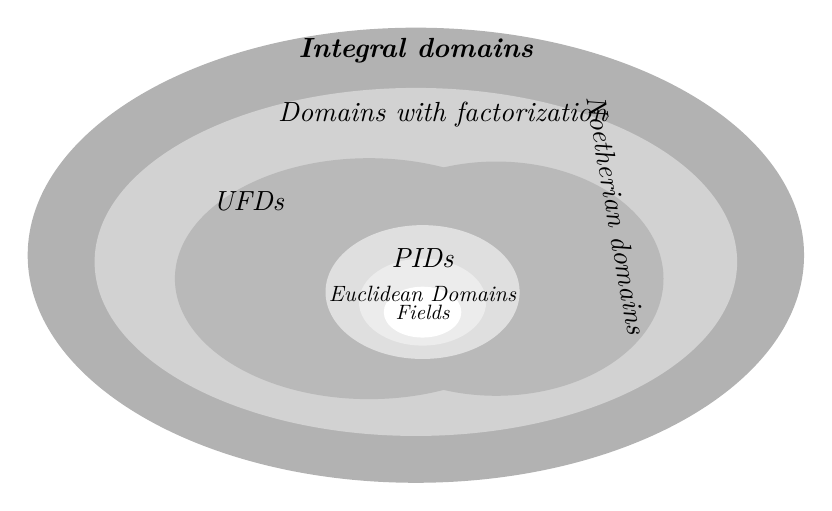
\begin{tikzpicture}[scale=0.85]
  \fill[gray!60] (0,0) ellipse (5.8cm and 3.4cm);
  \fill[gray!35] (0,-0.1) ellipse (4.8cm and 2.6cm);
  \fill[gray!55] (-0.7,-0.35) ellipse (2.9cm and 1.8cm);
  \fill[gray!55] (1.2,-0.35) ellipse (2.5cm and 1.75cm);
  \fill[gray!25] (0.1,-0.55) ellipse (1.45cm and 1.0cm);
  \fill[gray!15] (0.1,-0.7) ellipse (0.95cm and 0.65cm);
  \fill[white] (0.1,-0.85) ellipse (0.58cm and 0.38cm);
  \node[font=\bfseries\itshape] at (0,3.05) {Integral domains};
  \node[font=\itshape] at (0.4,2.1) {Domains with factorization};
  \node[font=\itshape] at (-2.5,0.8) {UFDs};
  \node[font=\itshape, rotate=-80] at (3.0,0.6) {Noetherian domains};
  \node[font=\itshape] at (0.1,-0.05) {PIDs};
  \node[font=\itshape, scale=0.8] at (0.1,-0.58) {Euclidean Domains};
  \node[font=\itshape, scale=0.75] at (0.1,-0.85) {Fields};
\end{tikzpicture}
\end{center}

\emph{Blanket assumption}: all rings considered in this chapter will be
\emph{commutative}\footnote{Also, recall that all our rings have 1; cf.\
Definition~III.1.1.}.  In fact, most of the special classes of rings we will
consider will be \emph{integral domains}, that is, commutative rings with 1
and with no nonzero zero-divisors (cf.\ Definition~III.1.10).

\section{Chain conditions and existence of factorizations}
\label{sec:irred:chain-conditions-and-existence-of-factorizations}


\subsection{Noetherian rings revisited}
\label{subsec:irred:noetherian-rings-revisited}

Let $R$ be a commutative ring. Recall that $R$ is said to be \emph{Noetherian}
if every ideal of $R$ is finitely generated (Definition~III.4.2). In fact,
this is a special case of the corresponding definition for modules: a module
$M$ over a ring $R$ is Noetherian if every submodule of $M$ is finitely
generated (Definition~III.6.6). In~\S{}III.6.4 we have verified that this
condition is preserved through exact sequences: if $M$, $N$, $P$ are
$R$-modules and
\[0 \longrightarrow N \longrightarrow M \longrightarrow P \longrightarrow 0\]
is an exact sequence of $R$-modules, then $M$ is Noetherian if and only if
both $N$ and $P$ are Noetherian (Proposition~III.6.7). An easy and useful
consequence of this fact is that every finitely generated module over a
Noetherian ring is Noetherian (Corollary~III.6.8).

The Noetherian condition may be expressed in alternative ways, and it is
useful to acquire some familiarity with them.
\begin{prop}{}{irred:1.1}
Let $R$ be a commutative ring, and let $M$ be an $R$-module. Then the
following are equivalent:
\begin{enumerate}[label=(\arabic*)]
\item $M$ is Noetherian; that is, every submodule of $M$ is finitely
  generated.
\item Every ascending chain of submodules of $M$ stabilizes; that is, if
  \[N_1 \subseteq N_2 \subseteq N_3 \subseteq \dots\]
  is a chain of submodules of $M$, then $\exists i$ such that
  $N_i = N_{i+1} = N_{i+2} = \dots$
\item Every nonempty family of submodules of $M$ has a maximal element
  w.r.t.\ inclusion.
\end{enumerate}
\end{prop}

The second condition listed here is called the \emph{ascending chain
condition} (a.c.c.) for submodules. For $M = R$, \cref{prop:irred:1.1}
tells us (among other things) that a ring is Noetherian if and only if the
ascending chain condition holds for its ideals.
\begin{proof}
$(1) \implies (2)$: Assume that $M$ is Noetherian, and let
$N_1 \subseteq N_2 \subseteq N_3 \subseteq \dots$ be a chain of submodules
of $M$. Consider the union $N = \bigcup_i N_i$: the reader will verify that
$N$ is a submodule of $M$. Since $M$ is Noetherian, $N$ is finitely
generated, say $N = \langle n_1, \dots, n_r \rangle$. Now $n_k \in N
\implies n_k \in N_i$ for some $i$; by picking the largest such $i$, we
see that $\exists i$ such that all $n_1, \dots, n_r$ are contained in
$N_i$. But then $N \subseteq N_i$, and since $N_i \subseteq N_{i+1}
\subseteq \dots$ are all contained in $N = N_i$, it follows that
$N_i = N_{i+1} = N_{i+2} = \dots$ as needed.

$(2) \implies (3)$: Arguing contrapositively, assume that $M$ admits a
family $\mathscr{F}$ of submodules that does not have a maximal element.
Construct an infinite ascending chain as follows: let $N_1$ be any element
of $\mathscr{F}$; since $N_1$ is not maximal in $\mathscr{F}$, there exists
an element $N_2$ of $\mathscr{F}$ such that $N_1 \subsetneq N_2$; since
$N_2$ is not maximal in $\mathscr{F}$, there exists an element $N_3$ of
$\mathscr{F}$ such that $N_2 \subsetneq N_3$; etc.\ The chain
$N_1 \subsetneq N_2 \subsetneq N_3 \subsetneq \dots$ does not stabilize,
showing that $(2)$ does not hold.

$(3) \implies (1)$: Assume $(3)$ holds, and let $N$ be a submodule of $M$.
Then the family $\mathscr{F}$ of finitely generated submodules of $N$ is
nonempty (as $(0) \in \mathscr{F}$); hence it has a maximal element $N'$.
Say that $N' = \langle n_1, \dots, n_r \rangle$. Now I claim that $N' = N$:
indeed, let $n \in N$; the submodule $\langle n_1, \dots, n_r, n \rangle$
is finitely generated, and therefore it is in $\mathscr{F}$; as it contains
$N'$ and $N'$ is maximal, necessarily $\langle n_1, \dots, n_r, n \rangle
= N'$; in particular $n \in N'$, as needed. This shows that $N = N'$ is
finitely generated, and since $N \subseteq M$ was arbitrary, this implies
that $M$ is Noetherian.
\end{proof}
Noetherian rings are a very useful and flexible class of rings. In~\S{}III.6.5
I mentioned the important fact that every \emph{finite-type algebra} over a
Noetherian ring is Noetherian. `Finite-type (commutative) algebra' is just a
fancy name for a quotient of a polynomial ring (\S{}III.6.5), so this is what
the fact states:

\begin{thm}{}{irred:1.2}
Let $R$ be a Noetherian ring, and let $J$ be an ideal of the polynomial ring
$R[x_1, \dots, x_n]$. Then the ring $R[x_1, \dots, x_n]/J$ is Noetherian.
\end{thm}

Note that finite-type $R$-algebras are (in general) very far from being
finitely generated as modules over $R$ (cf.\ again \S{}III.6.5), so it would
be foolish to expect them to be Noetherian as $R$-modules. The fact that they
turn out to be Noetherian as rings (that is, as modules over themselves)
provides us with a huge class of examples of Noetherian rings, among which are
the rings of (classical) algebraic geometry and number theory. Thus, entire
fields of mathematics are a little more manageable thanks to
\cref{thm:irred:1.2}.

The proof of this deep fact is surprisingly easy. By Exercise~1.1, it suffices
to prove that $R$ Noetherian $\implies$ $R[x_1, \dots, x_n]$ Noetherian; and
an immediate induction reduces the statement to the following particular case,
which carries a distinguished name:
\begin{lem}{Hilbert's basis theorem}{irred:1.3}
$R$ Noetherian $\implies$ $R[x]$ Noetherian.
\end{lem}

\begin{proof}
Assume $R$ is Noetherian, and let $I$ be an ideal of $R[x]$. We have to
prove that $I$ is finitely generated.

Recall that if $f(x) = a_d x^d + a_{d-1} x^{d-1} + \dots + a_0 \in R[x]$
and $a_d \neq 0$, then $a_d$ is called the \emph{leading coefficient} of
$f(x)$. Consider the following subset of $R$:
\[A = \{0\} \cup \{a \in R \mid a \text{ is a leading coefficient of an
  element of } I\}.\]
It is clear that $A$ is an ideal of $R$ (Exercise~1.6); since $R$ is
Noetherian, $A$ is finitely generated. Thus there exist elements
$f_1(x), \dots, f_r(x) \in I$ whose leading coefficients $a_1, \dots, a_r$
generate $A$ as an ideal of $R$.

Now let $d_i$ be the degree of $f_i(x)$, and let $d$ be the maximum among
these degrees. Consider the sub-$R$-module
\[M = \langle 1, x, x^2, \dots, x^{d-1} \rangle \subseteq R[x],\]
that is, the $R$-module consisting of polynomials of degree $< d$. Since
$M$ is finitely generated as a module over $R$, it is Noetherian as an
$R$-module (by Corollary~III.6.8). Therefore, the submodule $M \cap I$ of
$M$ is finitely generated over $R$, say by $g_1(x), \dots, g_s(x) \in I$.

\begin{fact}{Claim~1.4}{irred:claim:1.4}
$I = (f_1(x), \dots, f_r(x), g_1(x), \dots, g_s(x))$.
\end{fact}

This claim implies the statement of the theorem. To prove the claim, we
only need to prove the $\subseteq$ inclusion; to this end, let $\alpha(x)
\in I$ be an arbitrary polynomial in $I$. If $\deg\alpha(x) \geq d$, let
$a$ be the leading coefficient of $\alpha(x)$. Then $a \in A$, so $\exists
b_1, \dots, b_r \in R$ such that $a = b_1 a_1 + \dots + b_r a_r$. Letting
$e = \deg\alpha(x)$, so that $e \geq d_i$ for all $i$, this says that
\[\alpha(x) - b_1 x^{e-d_1} f_1(x) - \dots - b_r x^{e-d_r} f_r(x)\]
has degree $< e$. Iterating this procedure, we obtain a finite list of
polynomials $\beta_1(x), \dots, \beta_r(x) \in R[x]$ such that
\[\alpha(x) - \beta_1(x) f_1(x) - \dots - \beta_r(x) f_r(x)\]
has degree $< d$. But this places this element in $M \cap I$; therefore
$\exists c_1, \dots, c_s \in R$ such that
\[\alpha(x) - \beta_1(x)f_1(x) - \dots - \beta_r(x)f_r(x)
  = c_1 g_1(x) + \dots + c_s g_s(x),\]
and we are done, since this verifies that
\begin{align*}
\alpha(x) &= \beta_1(x)f_1(x) + \dots + \beta_r(x)f_r(x)
             + c_1 g_1(x) + \dots + c_s g_s(x) \\
          &\in (f_1(x), \dots, f_r(x), g_1(x), \dots, g_s(x)),
\end{align*}
completing the proof of \cref{fact:irred:claim:1.4}, hence of
\cref{lem:irred:1.3}, hence of \cref{thm:irred:1.2}.
\end{proof}

\subsection{Prime and irreducible elements}
\label{subsec:irred:prime-and-irreducible-elements}
Let $R$ be a (commutative) ring, and let $a, b \in R$. We say that $a$
\emph{divides} $b$, or that $a$ is a \emph{divisor} of $b$, or that $b$ is a
\emph{multiple} of $a$, if $b \in (a)$, that is,
\[(\exists c \in R),\quad b = ac.\]
We use the notation $a \mid b$.

Two elements $a$, $b$ are \emph{associates} if $(a) = (b)$, that is, if
$a \mid b$ and $b \mid a$.
\begin{lem}{}{irred:1.5}
Let $a$, $b$ be nonzero elements of an integral domain $R$. Then $a$ and
$b$ are associates if and only if $a = ub$, for $u$ a unit in $R$.
\end{lem}

\begin{proof}
Assume $a$ and $b$ are associates. Then $\exists c, d \in R$ such that
$b = ac$, $a = bd$; therefore $a = bd = acd$, i.e., $a(1 - cd) = 0$.
Since cancellation by nonzero elements holds in integral domains, this
implies $cd = 1$. Thus $c$ is a unit, as needed.

The converse is left to the reader.
\end{proof}
Incidentally, here the reader sees why it is convenient to restrict our
attention to integral domains. This argument really shows that if
$(a) = (b) \neq (0)$ in an integral domain, and $b = ca$, then $c$ is
necessarily a unit. Away from the comfortable environment of integral
domains, even such harmless-looking statements may fail: in $\mathbb{Z}/6\mathbb{Z}$
the classes $[2]_6$, $[4]_6$ of 2 and 4 are associates according to our
definition, and $[4]_6 = [2]_6 \cdot [2]_6$, yet $[2]_6$ is not a unit.
However, $[4]_6 = [5]_6 \cdot [2]_6$ and $[5]_6$ is a unit, so this is not
a counterexample to \cref{lem:irred:1.5}. In fact, \cref{lem:irred:1.5}
may fail over rings with `non-harmless' zero-divisors (yes, there is such a
notion).

The notions reviewed above generalize directly the corresponding notions in
$\mathbb{Z}$. We are going to explore analogues of other common notions in
$\mathbb{Z}$, such as `primality' and `irreducibility', in more general
integral domains.
\begin{defn}{}{irred:1.6}
Let $R$ be an integral domain.
\begin{itemize}
\item An element $a \in R$ is \emph{prime} if the ideal $(a)$ is prime;
  that is, $a$ is not a unit and (cf.\ Proposition~III.4.11)
  \[a \mid bc \implies (a \mid b \quad\text{or}\quad a \mid c).\]
\item An element $a \in R$ is \emph{irreducible} if $a$ is not a unit and
  \[a = bc \implies (b \text{ is a unit or } c \text{ is a unit}).\]
\end{itemize}
\end{defn}

Note that $0$ is always reducible (integral domains are nonzero rings!).
For nonzero elements, there are useful alternative ways to think about the
notion of `irreducible': a nonunit $a \neq 0$ is irreducible if and only if
\begin{itemize}
\item $a = bc$ implies that $a$ is an associate of $b$ or of $c$;
\item $a = bc$ implies that $(a) = (b)$ or $(a) = (c)$
  (\cref{lem:irred:1.5});
\item $(a) \subseteq (b) \implies (b) = (a)$ or $(b) = (1)$
  (Exercise~1.12);
\item $(a)$ is maximal among proper principal ideals (rephrasing the
  previous point!).
\end{itemize}

It is important to realize that primality and irreducibility are \emph{not}
equivalent, even for nonzero elements; this is somewhat counterintuitive
since they \emph{are} equivalent in $\mathbb{Z}$, as the reader should
verify\footnote{This fact will be fully explained by the general theory, so
the reader should work this out right away.} (Exercise~1.13). What is true
in general is that prime is stronger than irreducible:

\begin{lem}{}{irred:1.7}
Let $R$ be an integral domain, and let $a \in R$ be a nonzero prime
element. Then $a$ is irreducible.
\end{lem}

\begin{proof}
Since $(a)$ is prime, $(a) \neq (1)$; hence $a$ is not a unit. If
$a = bc$, then $bc = a \in (a)$; therefore $b \in (a)$ or $c \in (a)$
since $(a)$ is prime. Assuming without loss of generality $b \in (a)$, we
have $(b) \subseteq (a)$. On the other hand $a = bc$ implies
$(a) \subseteq (b)$: hence $(a) = (b)$, that is, $a$ and $b$ are
associates, as needed.
\end{proof}

We will soon see under what circumstances the converse statement holds.

\subsection{Factorization into irreducibles; domains with factorizations}
\label{subsec:irred:factorization-into-irreducibles-domains-with-factorizations}

\begin{defn}{}{irred:1.8}
Let $R$ be an integral domain. An element $r \in R$ has a \emph{factorization}
(or \emph{decomposition}) \emph{into irreducibles} if there exist irreducible
elements $q_1, \dots, q_n$ such that $r = q_1 \cdots q_n$.

This factorization is \emph{unique} if the elements $q_i$ are determined by
$r$ up to order and associates, that is, if whenever
$r = q'_1 \cdots q'_m$ is another factorization of $r$ into irreducibles,
then $m = n$ and $q'_i$ is an associate of $q_i$ after (possibly) shuffling
the factors.
\end{defn}

\begin{defn}{}{irred:1.9}
An integral domain $R$ is a \emph{domain with factorizations} (or
`\emph{factorizations exist in} $R$') if every nonzero, nonunit element
$r \in R$ has a factorization into irreducibles.
\end{defn}

\begin{defn}{}{irred:1.10}
An integral domain $R$ is \emph{factorial}, or a \emph{unique factorization
domain} (abbreviated \emph{UFD}), if every nonzero, nonunit element $r \in R$
has a unique factorization into irreducibles.
\end{defn}

The terminology introduced in \cref{defn:irred:1.9} does not appear to be too
standard; by contrast, UFDs are famous.

We will study the unique factorization condition in~\S{}2. For now, it seems
worth spending a little time contemplating the mere existence of
factorizations. Interestingly, this condition is implied by an ascending chain
condition, for a special class of ideals.

\begin{prop}{}{irred:1.11}
Let $R$ be an integral domain, and let $r$ be a nonzero, nonunit element of
$R$. Assume that every ascending chain of principal ideals
\[(r) \subseteq (r_1) \subseteq (r_2) \subseteq (r_3) \subseteq \dots\]
stabilizes. Then $r$ has a factorization into irreducibles.
\end{prop}

\begin{proof}
Assume that $r$ does not have a factorization into irreducible elements. In
particular, $r$ is itself not irreducible; thus $\exists r_1, s_1 \in R$ such
that $r = r_1 s_1$ and $(r) \subsetneq (r_1)$, $(r) \subsetneq (s_1)$. If
both $r_1$, $s_1$ have factorizations into irreducibles, the product of these
factorizations gives a factorization of $r$; thus we may assume that (e.g.)
$r_1$ does not have a factorization into irreducibles. Therefore we have
$(r) \subsetneq (r_1)$ and $r_1$ does not have a factorization; iterating
this argument constructs an infinitely increasing chain
\[(r) \subsetneq (r_1) \subsetneq (r_2) \subsetneq (r_3) \subsetneq \dots,\]
contradicting our hypothesis.
\end{proof}

Thus, factorizations exist in integral domains in which the ascending chain
condition holds for principal ideals. This has the following immediate and
convenient consequence:

\begin{coro}{}{irred:1.12}
Let $R$ be a Noetherian domain. Then factorizations exist in $R$.
\end{coro}

\begin{proof}
By \cref{prop:irred:1.1}, Noetherian domains satisfy the ascending chain
condition for all ideals.
\end{proof}

\cref{coro:irred:1.12} verifies part of the picture presented at the
beginning of the chapter: the class of Noetherian domains is contained in the
class of domains with factorization. This inclusion is proper: for instance,
the standard example of a non-Noetherian ring, $\mathbb{Z}[x_1, x_2, x_3,
\dots]$, (Example~III.6.5) does have factorizations. Indeed, every given
polynomial $f \in \mathbb{Z}[x_1, x_2, \dots]$ involves only finitely many
variables\footnote{Remember that polynomials are finite linear combinations
of monomials; cf.~\S{}III.1.3.}, so it belongs to a subring
$\mathbb{Z}[x_1, \dots, x_n]$ isomorphic to an ordinary polynomial ring over
$\mathbb{Z}$; further, this subring contains every divisor of $f$. It follows
easily (cf.\ Exercise~1.15) that the ascending chain condition for principal
ideals holds in $\mathbb{Z}[x_1, x_2, x_3, \dots]$, because it holds in
$\mathbb{Z}[x_1, \dots, x_n]$ (since this ring is Noetherian, by Hilbert's
basis theorem).

\subsection*{Exercises}

Remember that in this section all rings are taken to be \emph{commutative}.
\begin{exer}{\exerused}{exer:irred:1.1}
Let $R$ be a Noetherian ring, and let $I$ be an ideal of $R$. Prove that
$R/I$ is a Noetherian ring. [\S{}1.1]
\end{exer}

\begin{exer}{}{exer:irred:1.2}
Prove that if $R[x]$ is Noetherian, so is $R$. (This is a `converse' to
Hilbert's basis theorem.)
\end{exer}

\begin{exer}{}{exer:irred:1.3}
Let $k$ be a field, and let $f \in k[x]$, $f \notin k$. For every subring
$R$ of $k[x]$ containing $k$ and $f$, define a homomorphism $\phi : k[t]
\to R$ by extending the identity on $k$ and mapping $t$ to $f$. This makes
every such $R$ a $k[t]$-algebra (Example~III.5.6).
\begin{itemize}
\item Prove that $k[x]$ is finitely generated as a $k[t]$-module.
\item Prove that every subring $R$ as above is finitely generated as a
  $k[t]$-module.
\item Prove that every subring of $k[x]$ containing $k$ is a Noetherian
  ring.
\end{itemize}
\end{exer}

\begin{exer}{}{exer:irred:1.4}
Let $R$ be the ring of real-valued continuous functions on the interval
$[0, 1]$. Prove that $R$ is not Noetherian.
\end{exer}

\begin{exer}{}{exer:irred:1.5}
Determine for which sets $S$ the power set ring $\mathscr{P}(S)$ is
Noetherian. (Cf.\ Exercise~III.3.16.)
\end{exer}
\begin{exer}{\exerused}{exer:irred:1.6}
Let $I$ be an ideal of $R[x]$, and let $A \subseteq R$ be the set defined
in the proof of \cref{thm:irred:1.2}. Prove that $A$ is an ideal of $R$.
[\S{}1.1]
\end{exer}

\begin{exer}{}{exer:irred:1.7}
Prove that if $R$ is a Noetherian ring, then the ring of power series
$R[[x]]$ (cf.~\S{}III.1.3) is also Noetherian. (Hint: The order of a power
series $\sum_{i=0}^{\infty} a_i x^i$ is the smallest $i$ for which $a_i
\neq 0$; the dominant coefficient is then $a_i$. Let $A_i \subseteq R$ be
the set of dominant coefficients of series of order $i$ in $I$, together
with $0$. Prove that $A_i$ is an ideal of $R$ and $A_0 \subseteq A_1
\subseteq A_2 \subseteq \dots$. This sequence stabilizes since $R$ is
Noetherian, and each $A_i$ is finitely generated for the same reason. Now
adapt the proof of \cref{lem:irred:1.3}.)
\end{exer}
\begin{exer}{}{exer:irred:1.8}
Prove that every ideal in a Noetherian ring $R$ contains a finite product
of prime ideals. (Hint: Let $\mathscr{F}$ be the family of ideals that do
not contain finite products of prime ideals. If $\mathscr{F}$ is nonempty,
it has a maximal element $M$ since $R$ is Noetherian. Since $M \in
\mathscr{F}$, $M$ is not itself prime, so $\exists a, b \in R$ s.t.\ $a
\notin M$, $b \notin M$, yet $ab \in M$. What's wrong with this?)
\end{exer}
\begin{exer}{$\lnot$}{exer:irred:1.9}
Let $R$ be a commutative ring, and let $I \subseteq R$ be a proper ideal.
The reader will prove in Exercise~3.12 that the set of prime ideals
containing $I$ has minimal elements (the \emph{minimal primes} of $I$).
Prove that if $R$ is Noetherian, then the set of minimal primes of $I$ is
finite. (Hint: Let $\mathscr{F}$ be the family of ideals that do not have
finitely many minimal primes. If $\mathscr{F} \neq \emptyset$, note that
$\mathscr{F}$ must have a maximal element $I$, and $I$ is not prime itself.
Find ideals $J_1$, $J_2$ strictly larger than $I$, such that $J_1 J_2
\subseteq I$, and deduce a contradiction.) [\hyperref[exer:linAlg:4.10]{VI.4.10}]
\end{exer}
\begin{exer}{$\lnot$}{exer:irred:1.10}
By \cref{prop:irred:1.1}, a ring $R$ is Noetherian if and only if it
satisfies the a.c.c.\ for ideals. A ring is \emph{Artinian} if it
satisfies the d.c.c.\ (descending chain condition) for ideals. Prove that
if $R$ is Artinian and $I \subseteq R$ is an ideal, then $R/I$ is Artinian.
Prove that if $R$ is an Artinian integral domain, then it is a field.
(Hint: Let $r \in R$, $r \neq 0$. The ideals $(r^n)$ form a descending
sequence; hence $(r^n) = (r^{n+1})$ for some $n$. Therefore\dots) Prove
that Artinian rings have Krull dimension $0$ (that is, prime ideals are
maximal in Artinian rings\footnote{One can prove that Artinian rings are
necessarily Noetherian; in fact, a ring is Artinian if and only if it is
Noetherian and has Krull dimension $0$. Thus, the d.c.c.\ implies the
a.c.c., while the a.c.c.\ implies the d.c.c.\ if and only if all prime
ideals are maximal.}). [\hyperref[exer:irred:2.11]{2.11}]
\end{exer}

\begin{exer}{}{exer:irred:1.11}
Prove that the `associate' relation is an equivalence relation.
\end{exer}

\begin{exer}{\exerused}{exer:irred:1.12}
Let $R$ be an integral domain. Prove that a nonzero $a \in R$ is
irreducible if and only if $(a)$ is maximal among proper principal ideals
of $R$. [\S{}1.2, \S{}2.3]
\end{exer}

\begin{exer}{\exerused}{exer:irred:1.13}
Prove that, for nonzero elements, prime $\iff$ irreducible in $\mathbb{Z}$.
[\S{}1.2, \S{}2.3]
\end{exer}

\begin{exer}{}{exer:irred:1.14}
For $a$, $b$ in a commutative ring $R$, prove that the class of $a$ in
$R/(b)$ is prime if and only if the class of $b$ in $R/(a)$ is prime.
\end{exer}

\begin{exer}{\exerused}{exer:irred:1.15}
Identify $S = \mathbb{Z}[x_1, \dots, x_n]$ in the natural way with a
subring of the polynomial ring in countably infinitely many variables
$R = \mathbb{Z}[x_1, x_2, x_3, \dots]$. Prove that if $f \in S$ and
$(f) \subseteq (g)$ in $R$, then $g \in S$ as well. Conclude that the
ascending chain condition for principal ideals holds in $R$, and hence $R$
is a domain with factorizations. [\S{}1.3, \S{}4.3]
\end{exer}

\begin{exer}{}{exer:irred:1.16}
Let
\[R = \frac{\mathbb{Z}[x_1, x_2, x_3, \dots]}{(x_1 - x_2^2,\, x_2 -
x_3^2,\, \dots)}.\]
Does the ascending chain condition for principal ideals hold in $R$?
\end{exer}

\begin{exer}{\exerused}{exer:irred:1.17}
Consider the subring of $\mathbb{C}$:
\[\mathbb{Z}[\sqrt{-5}] := \{a + bi\sqrt{5} \mid a, b \in \mathbb{Z}\}.\]
\begin{itemize}
\item Prove that this ring is isomorphic to $\mathbb{Z}[t]/(t^2 + 5)$.
\item Prove that it is a Noetherian integral domain.
\item Define a `norm' $N$ on $\mathbb{Z}[\sqrt{-5}]$ by setting
  $N(a + bi\sqrt{5}) = a^2 + 5b^2$. Prove that $N(zw) = N(z)N(w)$.
  (Cf.\ Exercise~III.4.10.)
\item Prove that the units in $\mathbb{Z}[\sqrt{-5}]$ are $\pm 1$. (Use
  the preceding point.)
\item Prove that $2$, $3$, $1 + i\sqrt{5}$, $1 - i\sqrt{5}$ are all
  irreducible nonassociate elements of $\mathbb{Z}[\sqrt{-5}]$.
\item Prove that no element listed in the preceding point is prime. (Prove
  that the rings obtained by mod-ing out the ideals generated by these
  elements are not integral domains.)
\item Prove that $\mathbb{Z}[\sqrt{-5}]$ is not a UFD.
\end{itemize}
[\S{}2.2, \hyperref[exer:irred:2.18]{2.18},
\hyperref[exer:irred:6.14]{6.14}]
\end{exer}

\section{UFDs, PIDs, Euclidean domains}
\label{sec:irred:ufds-pids-euclidean-domains}


\subsection{Irreducible factors and greatest common divisor}
\label{subsec:irred:irreducible-factors-and-greatest-common-divisor}
% An integral domain

% R is a UFD if factorizations exist in R and are unique in the sense of
% Definition 1.8.
% Thus, in a UFD all elements (other than 0 and the units) determine a multiset
% (a set of elements `with multiplicity'; cf. \S{}I.1.1) of irreducible factors,
% determined
% up to the associate relation. We can also agree that units have no factors; that
% is,
% the corresponding multiset is \emptyset .
% The following trivial remark is at the root of most elementary facts about
% UFDs, such as the characterization of Theorem 2.5:
% Lemma 2.1. Let R be a UFD, and let a, b, c be nonzero elements of R. Then
% \bullet  (a) \subseteq  (b) \iff  the multiset of irreducible factors of b is contained in the
% multiset of irreducible factors of a;
% \bullet  a and b are associates (that is, (a) = (b)) \iff  the two multisets coincide;
% \bullet  the irreducible factors of a product bc are the collection of all irreducible factors
% of b and of c.
% The proof is left to the reader (Exercise 2.1). The advantage of working in
% a UFD resides in the fact that ring-theoretic statements about elements of the
% ring often reduce to straightforward set-theoretic statements about multisets of
% irreducible elements, by means of Lemma 2.1.
% One important instance of this mechanism is the existence of greatest common
% divisors. I have liberally used this notion (at least for integers) in previous
% chapters;
% now we can appreciate it from a more technical perspective.
% Definition 2.2. Let R be an integral domain, and let a, b \in  R. An element d
% \in  R
% is a greatest common divisor (often abbreviated `gcd') of a and b if (a, b)
% \subseteq  (d) and
% (d) is the smallest principal ideal in R with this property.
%  ?
% In other words, d is a gcd of a and b if d | a, d | b, and
% c | a , c | b \implies  c | d.
% This definition is immediately extended to any finite number of elements.
% Note that greatest common divisors are not defined uniquely by this prescrip-
% tion: if d is a greatest common divisor of a and b, so is every associate of d.
% Thus,
% the notation `gcd(a, b)' should only be used for the associate class formed by
% all
% greatest common divisors of a, b. Of course, language is often (harmlessly)
% abused
% on this point. For example, the fact that we can talk about the greatest common
% divisor of two integers is due to the fact that in Z there is a convenient way
% to choose
% a distinguished element in each class of associate integers (that is, the
% nonnegative
% one).
% Also note that greatest common divisors need not exist (cf. Exercise 2.5); but
% they do exist in UFDs:
% Lemma 2.3. Let R be a UFD, and let a, b be nonzero elements of R. Then a, b
% have a greatest common divisor.
% Proof. We can write
% a = uq1 \alpha 1 \dots  qr \alpha r ,
%  b = vq1 \beta 1 \dots  qr \beta r
% where u and v are units, the elements qi are irreducible, qi is not an associate
% of qj
% for i = j, and \alpha i \geq  0, \beta i \geq  0 (so that the multisets of
% irreducible factors of a,
% resp., b, consist of those qi for which \alpha i > 0, resp., \beta i > 0; the
% units u, v are
% included since the irreducible factors are only defined up to the associate
% relation).
% I claim that
% d = q1
%  min(\alpha 1 ,\beta 1
%  )
%  \dots  qr min(\alpha r ,\beta r )
% is a gcd of a and b. Indeed, d is clearly a divisor of a and b; and if c also
% divides
% a and b, then the multiset of factors of c must be contained in both multisets
% of
% factors for a and b (by Lemma 2.1); that is,
% c = wq1 \gamma 1 \dots  qr \gamma r
% with w a unit and \gamma i \leq  \alpha i , \gamma i \leq  \beta  i . This
% implies \gamma i \leq  min(\alpha i , \beta i ), and hence c | d
% (again by Lemma 2.1), as needed.
%  ?
% Of course the argument given in the proof generalizes one of the standard
% ways to compute greatest common divisors in Z: find smallest exponents in prime
% factorizations. But note that this is not the only way to compute the gcd in Z;
% we will come back to this point in a moment. In fact, greatest common divisors
% in Z have properties that should not be expected in a more general domain: for
% example, the result of Exercise II.2.13 does not generalize to arbitrary domains
% (and not even to arbitrary UFDs), as the reader will check in Exercise 2.4.

\subsection{Characterization of UFDs}
\label{subsec:irred:characterization-of-ufds}
% It is easy to construct integral domains where

% unique factorization fails. The diligent reader has already analyzed one example
% (Exercise 1.17); for another, in the domain5
% C[x, y, z, w]
% R =
% (xw - yz)
% the (classes of the) elements x, y, z, w are irreducible and not associates of
% one
% another; since xw - yz = 0 in R, the element r = xw has two distinct
% factorizations
% into irreducibles: r = xw = yz.
% Note that this ring is Noetherian, by Theorem 1.2 (and in particular factor-
% izations do exist in R). Thus, there are Noetherian integral domains that are
% not
% UFDs.
% Also note that this ring provides an example in which the converse to Lemma 1.7
% does not hold: indeed, (the class of) x is irreducible, but the quotient
% '
% C[x, y, z, w]
%  C[x, y, z, w]
%  C[x, y, z, w]
% (x) \sim 
%  =
%  =
% (xw - yz)
%  (x, xw - yz)
%  (x, yz)
% is not an integral domain (because y = 0, z = 0, and yet yz = 0 in this ring);
% that
% is, x is not prime.
% In fact, and maybe a little surprisingly, the issue of unique factorization is
% inextricably linked with the relation between primality and irreducibility.
% Indeed,
% the `converse' to Lemma 1.7 does hold in UFDs:
% Lemma 2.4. Let R be a UFD, and let a be an irreducible element of R. Then a
% is prime.
% Proof. The element a is not a unit, by definition of irreducible. Assume bc \in
% (a):
% thus (bc) \subseteq  (a), and by Lemma 2.1 the irreducible factors of a, that
% is, a itself,
% must be among the factors of b or of c. We have b \in  (a) in the first case and
% c \in  (a)
% in the second. This shows that (a) is a prime ideal, as needed.
%  ?
% In fact, more is true. Provided that the ascending chain condition for principal
% ideals holds, then UFDs are characterized by the equivalence between
% irreducibility
% and primality.
% Theorem 2.5. An integral domain R is a UFD if and only if
% \bullet  the a.c.c. for principal ideals holds in R and
% \bullet  every irreducible element of R is prime.
% Proof. ( \implies  ) Assume that R is a UFD. Lemma 2.4 shows that irreducible
% ele-
% ments of R are prime. To prove that the a.c.c. for principal ideals holds,
% consider
% an ascending chain
% (r1 ) ? (r2 ) ? (r3 ) ? \dots  .
% 5 In algebraic geometry, this is the ring of a `quadric cone in A4'. The vertex
% of this cone (at
% the origin) is a singular point, and this has to do with the fact that R is not
% a UFD.
% By Lemma 2.1, this chain determines a corresponding descending chain of
% multisets
% of irreducible factors. A descending chain of finite multisets clearly
% stabilizes, and it
% follows (by Lemma 2.1 again) that (ri ) = (ri+1 ) = (ri+2 ) = . . . for large
% enough i.
% ( \Leftarrow = ) Now assume that R satisfies the a.c.c. for principal ideals and
% irre-
% ducibles are prime. Proposition 1.11 implies that factorizations exist in R; we
% have
% \setminus  \setminus to verify uniqueness. Let q1 , . . . , qm and q1 , . . . , qn be irreducible elements of R,
% and assume
% q1 \dots  qm = q1 \setminus  \dots  qn \setminus  .
% Then q1 \setminus  \dots  qn \setminus  \in  (q1 ), and (q1 ) is a prime ideal
% (by hypothesis); thus qi \setminus  \in  (q1)
% for some i, which we may assume to be 1 after changing the order of the factors.
% Therefore q1 \setminus  = uq1 for some u \in  R. Since q1 \setminus  is
% irreducible and q1 is not a unit,
% \setminus  \setminus 
% necessarily u is a unit. Thus q1 and q1 are associates. Canceling q1 and
% replacing q2\setminus by uq2, we find
% q2 \dots  qm = q2 \setminus  \dots  qn \setminus  .
% Repeating this process matches all factors one by one. It is clear that m = n,
% because otherwise we will obtain 1 = a product of irreducibles, contradicting
% the
% fact that irreducibles are not units.
%  ?
% Theorem 2.5 is a pleasant statement, but it does not make it particularly easy
% to
% check whether a given ring is in fact a UFD. The situation is not unlike that
% with
% Noetherian rings: the a.c.c. is a sharp equivalent formulation of the Noetherian
% condition, but in practice one relies more often on other tools, such as
% Hilbert's
% basis theorem, in order to establish that a given ring is Noetherian. Does an
% analog
% of Hilbert's basis theorem hold for unique factorization domains?
% Answering this question requires some preparatory work, and we will come back
% to it in \S{}4.

\subsection{\texorpdfstring{PID $\implies$ UFD}{PID implies UFD}}
\label{subsec:irred:pid-implies-ufd}
% There are simple ways to produce examples of UFDs.

% Recall (from \S{}III.4) that a principal ideal domain (abbreviated PID) is an
% integral
% domain in which every ideal is principal. In \S{}III.4 we have observed that
% \bullet  PIDs are Noetherian.
% \bullet  Z and k[x] (where k is a field) are PIDs.
% \bullet  If R is a PID and a, b \in  R, then d is a greatest common divisor for a and b if
% and only if (a, b) = (d). In particular, if d is a greatest common divisor of a
% and b in a PID R, then d is a linear combination of a and b: \exists r, s \in  R
% such
% that d = ra + sb.
% \bullet  If I is a nonzero ideal in a PID, then I is prime if and only if it is maximal.
% We now add one important point to this list:
% Proposition 2.6. If R is a PID, then it is a UFD.
% Proof. Let R be a PID. The a.c.c. (for principal ideals, as all ideals in R are
% prin-
% cipal!) holds in R since PIDs are Noetherian. We verify that irreducible
% elements
% are prime in R, which implies that R is a UFD by Theorem 2.5.
% Let a \in  R be an irreducible element. Ideals generated by irreducible elements
% are maximal among principal ideals (Exercise 1.12), hence (a) is a maximal ideal
% in R as all ideals in R are principal. Since maximal ideals are prime it follows
% that
% (a) is prime, as needed.
%  ?
% In particular, k[x] is a UFD if k is a field, and Z is a UFD---which hopefully
% will not come as a big surprise to our readers6. Note that at this point we have
% recovered the fact stated in Exercise 1.13 in full glory.
% Proposition 2.6 justifies another feature of the picture given at the beginning
% of this chapter: the class of PIDs is contained in the class of UFDs. We will
% soon
% see that the inclusion is proper, that is, that there are UFDs which are not
% PIDs;
% for example, Z[x] is not a PID (Exercise 2.12), yet
% Z[x] is a unique factorization domain
% as we will soon be able to prove (Theorem 4.14). In fact, there are UFDs which
% are not Noetherian, as represented in the picture; however, these examples are
% best
% discussed after more material has been developed (Example 4.18).
% The reader can already get a feel for the gap between UFD and PID, by con-
% templating the fact (recalled above and essentially tautological) that, in a
% PID,
% greatest common divisors of a, b are linear combinations of a and b. This is a
% very strong requirement: for example, it characterizes PIDs among Noetherian do-
% mains, as the reader will check (Exercise 2.7); it does not hold in general UFDs
% (Exercise 2.4).

\subsection{\texorpdfstring{Euclidean domain $\implies$ PID}{Euclidean domain implies PID}}
\label{subsec:irred:euclidean-domain-implies-pid}
% The excellent properties of Z and k[x] (where

% k is a field) make these rings even more special than PIDs: they are Euclidean
% domains.
% Informally, Euclidean domains are rings in which one may perform a `division
% with remainder': this is the case for Z and for k[x], as observed in \S{}III.4.
% The point
% is that in both Z and k[x] one can define a notion of `size' of an element: |n|
% for an
% integer n and deg f (x) for a polynomial f (x). In both cases, one has control
% over
% the size of the `remainder' in a division. The definition of Euclidean domain
% simply
% abstracts this mechanism.
% For the purpose of this discussion7 , a valuation on an integral domain R is any
% function v : R \setminus  {0} \to  Z\geq 0 .
% Definition 2.7. A Euclidean valuation on an integral domain R is a valuation
% satisfying the following property 8 : for all a \in  R and all nonzero b \in  R
% there exist
% q, r \in  R such that
% a = qb + r,
% with either r = 0 or v(r) < v(b). An integral domain R is a Euclidean domain if
% it
% admits a Euclidean valuation.
%  ?
% 6This fact is known as the fundamental theorem of arithmetic.
% 7 Entire libraries have been written on the subject of valuations, studying a
% more precise
% notion than what is needed here.
% 8 It is not uncommon to also require that v(ab) \geq  v(b) for all nonzero a, b
% \in  R; but this is not
% needed in the considerations that follow, and cf. Exercise 2.15.
% We say that q is the quotient of the division and r is the remainder. Division
% with remainder in Z and in k[x] (where k is a field) provide examples, so that Z
% and k[x] are Euclidean domains.
% Proposition 2.8. Let R be a Euclidean domain. Then R is a PID.
% The proof is modeled after the instances encountered for Z (Proposition III.4.4)
% and k[x] (which the reader has hopefully worked out in Exercise III.4.4).
% Proof. Let I be an ideal of R; we have to prove that I is principal. If I = {0},
% there is nothing to show; therefore, assume I = {0}. The valuation maps the
% nonzero elements of I to a subset of Z\geq 0 ; let b \in  I be an element with
% the smallest
% valuation. Then I claim that I = (b); therefore I is principal, as needed. Since
% clearly (b) \subseteq  I, we only need to verify that I \subseteq  (b).
% For this, let a \in  I and apply division with remainder: we have
% a = qb + r
% for some q, r in R, with r = 0 or v(r) < v(b). But
% r = a - qb \in  I :
% by the minimality of v(b) among nonzero elements of I, we cannot have v(r) <
% v(b).
% Therefore r = 0, showing that a = qb \in  (b), as needed.
%  ?
% Proposition 2.8 justifies one more feature of the picture at the beginning of
% the
% chapter: the class of Euclidean domains is contained in the class of principal
% ideal
% domains.
% This inclusion is proper, as suggested in the picture. Producing an explicit
% example of a PID which is not a Euclidean domain is not so easy, but the gap
% between PIDs and Euclidean domains can in fact be described very sharply: PID
% may be characterized as domains satisfying a weaker requirement than `division
% with remainder'.
% More precisely, a `Dedekind-Hasse valuation' is a valuation v such that \forall
% a, b,
% either (a, b) = (b) (that is, b divides a) or there exists r \in  (a, b) such
% that v(r) < v(b).
% This latter condition amounts to requiring that there exist q, s \in  R such
% that
% as = bq + r with v(r) < v(b); hence a Euclidean valuation (for which we may in
% fact
% choose s = 1) is a Dedekind-Hasse valuation. It is not hard to show that an
% integral
% domain is a PID if and only if it admits a Dedekind-Hasse valuation
%  \sqrt 
%  (Exercise 2.21).
% For example, this can be used to show that the ring Z[(1 + -19)/2] is a PID: the
% norm considered in Exercise 2.18 in order to prove that this ring is not a
% Euclidean
% domain turns out to be a Dedekind-Hasse valuation9 . Thus, this ring gives an
% example of a PID that is not a Euclidean domain.
% One excellent feature of Euclidean domains, and the one giving them their
% names, is the presence of an effective algorithm computing greatest common divi-
% sors: the Euclidean algorithm. As Euclidean domains are PIDs, and hence UFDs,
% we know that they do have greatest common divisors. However, the `algorithm'
% 9 This boils down to a case-by-case analysis, which I am happily leaving to my
% most patient
% readers.
% obtained by distilling the proof of Lemma 2.3 is highly impractical: if we had
% to
% factor two integers a, b in order to compute their gcd, this would make it
% essentially
% impossible (with current technologies and factorization algorithms) for integers
% of
% a few hundred digits. The Euclidean algorithm bypasses the necessity of
% factoriza-
% tion: greatest common divisors of thousand-digit integers may be computed in a
% fraction of a second.
% The key lemma on which the algorithm is based is the following trivial general
% fact:
% Lemma 2.9. Let a = bq + r in a ring R. Then (a, b) = (b, r).
% Proof. Indeed, r = a - bq \in  (a, b), proving (b, r) \subseteq  (a, b); and a =
% bq + r \in  (b, r),
% proving (a, b) \subseteq  (b, r).
%  ?
% In particular,
% (\forall c \in  R),
%  (a, b) \subseteq  (c) \iff  (b, r) \subseteq  (c);
% that is, the set of common divisors of a, b and the set of common divisors of b,
% r
% coincide. Therefore,
% Corollary 2.10. Assume a = bq + r. Then a, b have a gcd if and only if b, r have
% a gcd, and in this case gcd(a, b) = gcd(b, r).
% Of course `gcd(a, b) = gcd(b, r)' means that the two classes of associate
% elements
% coincide.
% These considerations hold over any integral domain; assume now that R is a
% Euclidean domain. Then we can use division with remainder to gain some control
% over the remainders r. Given two elements a, b in R, with b = 0, we can apply
% division with remainder repeatedly:
% a = bq1 + r1 ,
% b = r1 q2 + r2 ,
% r1 = r2 q3 + r3 ,
% \cdot \cdot \cdot 
% as long as the remainder ri is nonzero.
% Claim 2.11. This process terminates: that is, rN = 0 for some N .
% Proof. Each line in the table is a division with remainder. If no ri were zero,
% we
% would have an infinite decreasing sequence
% v(b) > v(r1) > v(r2 ) > v(r3) > \dots 
% of nonnegative integers, which is nonsense.
%  ?
% Thus the table of divisions with remainders must be as follows: letting r0 = b,
% a = r0 q1 + r1 ,
% b = r1 q2 + r2 ,
% r1 = r2 q3 + r3 ,
% \cdot \cdot \cdot 
% rN -3 = rN -2 qN -1 + rN -1 ,
% rN -2 = rN -1 qN
% with rN -1 = 0.
% Proposition 2.12. With notation as above, rN -1 is a gcd of a, b.
% Proof. By Corollary 2.10,
% gcd(a, b) = gcd(b, r1 ) = gcd(r1 , r2 ) = \dots  = gcd(rN -2 , rN -1 ).
% But rN -2 = rN -1 qN -1 gives rN -2 \in  (rN -1 ); hence (rN -2 , rN -1 ) = (rN
% -1 ). There-
% fore rN -1 is a gcd for rN -2 and rN -1 , hence for a and b, as needed.
%  ?
% The ring of integers and the polynomial ring over a field are both Euclidean
% domains. Fields are Euclidean domains (as represented in the picture at the be-
% ginning of the chapter), but not for a very interesting reason: the remainder of
% the
% division by a nonzero element in a field is always zero, so every function
% qualifies
% as a `Euclidean valuation' for trivial reasons.
% We will study another interesting Euclidean domain later in this chapter
% (\S{}6.2).

\subsection*{Exercises}

% 2.1. ? Prove Lemma 2.1. [\S{}2.1]
% 2.2. Let R be a UFD, and let a, b, c be elements of R such that a | bc and
% gcd(a, b) =
% 2.3. Let n be a positive integer. Prove that there is a one-to-one
% correspondence
% preserving multiplicities between the irreducible factors of n (as an integer)
% and
% the composition factors of Z/nZ (as a group). (In fact, the Jordan-H\"older
% theorem
% may be used to prove that Z is a UFD.)
% 2.4. ? Consider the elements x, y in Z[x, y]. Prove that 1 is a gcd of x and y,
% and
% yet 1 is not a linear combination of x and y. (Cf. Exercise II.2.13.) [\S{}2.1,
% \S{}2.3]
% 2.5. ? Let R be the subring of Z[t] consisting of polynomials with no term of
% degree 1: a0 + a2 t2 + \dots  + adtd .
% \bullet  Prove that R is indeed a subring of Z[t], and conclude that R is an integral
% domain.
% \bullet  List all common divisors of t5 and t6 in R.
% \bullet  Prove that t5 and t6 have no gcd in R.
% [\S{}2.1]
% 2.6. Let R be a domain with the property that the intersection of any family of
% principal ideals in R is necessarily a principal ideal.
% \bullet  Show that greatest common divisors exist in R.
% \bullet  Show that UFDs satisfy this property.
% 2.7. ? Let R be a Noetherian domain, and assume that for all nonzero a, b in R,
% the greatest common divisors of a and b are linear combinations of a and b.
% Prove
% that R is a PID. [\S{}2.3]
% 2.8. Let R be a UFD, and let I = (0) be an ideal of R. Prove that every
% descending
% chain of principal ideals containing I must stabilize.
% 2.9. \lnot  The height of a prime ideal P in a ring R is (if finite) the maximum
% length h
% of a chain of prime ideals P0 ? P1 ? \dots  ? Ph = P in R. (Thus, the Krull
% dimension
% of R, if finite, is the maximum height of a prime ideal in R.) Prove that if R
% is a
% UFD, then every prime ideal of height 1 in R is principal. [2.10]
% 2.10. \lnot  It is a consequence of a theorem known as Krull's Hauptidealsatz
% that
% every nonzero, nonunit element in a Noetherian domain is contained in a prime
% ideal of height 1. Assuming this, prove a converse to Exercise 2.9, and conclude
% that a Noetherian domain R is a UFD if and only if every prime ideal of height 1
% in R is principal. [4.16]
% 2.11. Let R be a PID, and let I be a nonzero ideal of R. Show that R/I is an
% artinian ring (cf. Exercise 1.10), by proving explicitly that the d.c.c. holds
% in R/I.
% 2.12. ? Prove that if R[x] is a PID, then R is a field. [\S{}2.3, \S{}VI.7.1]
% 2.13. ? For a, b, c positive integers with c > 1, prove that ca - 1 divides cb -
% 1 if
% and only if a | b. Prove that xa - 1 divides xb - 1 in Z[x] if and only if a |
% b. (Hint:
% For the interesting implications, write b = ad + r with 0 \leq  r < a, and take
% `size'
% into account.) [\S{}VII.5.1, VII.5.13]
% 2.14. ? Prove that if k is a field, then k[[x]] is a Euclidean domain. [\S{}4.3]
% 2.15. ? Prove that if R is a Euclidean domain, then R admits a Euclidean valua-
% tion v such that v(ab) \geq  v(b) for all nonzero a, b \in  R. (Hint: Since R is
% a Euclidean
% domain, it admits a valuation v as in Definition 2.7. For a = 0, let v(a) be the
% minimum of all v(ab) as b \in  R, b = 0. To see that R is a Euclidean domain
% with
% respect to v as well, let a, b be nonzero in R, with b ? a; choose q, r so that
% a = bq+r,
% with v(r) minimal; assume that v(r) \geq  v(b), and get a contradiction.)
% [\S{}2.4, 2.16]
% 2.16. Let R be a Euclidean domain with Euclidean valuation v; assume that
% v(ab) \geq  v(b) for all nonzero a, b \in  R (cf. Exercise 2.15). Prove that
% associate
% elements have the same valuation and that units have minimum valuation.
% 2.17. \lnot  Let R be a Euclidean domain that is not a field. Prove that there
% exists a
% nonzero, nonunit element c in R such that \forall a \in  R, \exists q, r \in  R
% with a = qc + r and
% either r = 0 or r a unit. [2.18]
% \sqrt 
% 2.18. ? For an integer d, denote by Q( d) the smallest subfield of C containing
% \sqrt Q and d, with norm N defined as in Exercise III.4.10. See Exercise 1.17 for the
% case d = -5; in this problem, you will take d = -19.
% \sqrt 
%  \sqrt 
% Let \delta  = (1 + i 19)/2, and consider the following subring of Q( -19):
% ?
%  \sqrt 
% 1 + i 19
% Z[\delta ] := a + b
%  | a, b \in  Z .
% \bullet  Prove that the smallest values of N (z) for z = a + b\delta  \in  Z[\delta ] are 0, 1, 4, 5. Prove
% that N (a + b\delta ) \geq  5 if b = 0.
% \bullet  Prove that the units in Z[\delta ] are \pm 1.
% \bullet  If c \in  Z[\delta ] satisfies the condition specified in Exercise 2.17, prove that c must
% divide 2 or 3 in Z[\delta ], and conclude that c = \pm 2 or c = \pm 3.
% \bullet  Now show that ?q \in  Z[\delta ] such that \delta  = qc + r with c = \pm 2, \pm 3 and r = 0, \pm 1.
% \sqrt 
% Conclude that Z[(1 + -19)/2] is not a Euclidean domain. [\S{}2.4, 6.14]
% 2.19. \lnot  A discrete valuation on a field k is a surjective homomorphism of
% abelian
% groups v : (k\ast  , \cdot ) \to  (Z, +) such that v(a + b) \geq  min(v(a),
% v(b)) for all a, b \in  k\ast  such
% that a + b \in  k\ast  .
% \bullet  Prove that the set R := {a \in  k \ast  | v(a) \geq  0} \cup  {0} is a subring of k.
% \bullet  Prove that R is a Euclidean domain.
% Rings arising in this fashion are called discrete valuation rings, abbreviated
% DVR.
% They arise naturally in number theory and algebraic geometry. Note that the
% Krull dimension of a DVR is 1 (Example III.4.14); in algebraic geometry, DVRs
% correspond to particularly nice points on a `curve'.
% \bullet  Prove that the ring of rational numbers a/b with b not divisible by a fixed prime
% integer p is a DVR.
% [2.20, VIII.1.19]
% 2.20. \lnot  As seen in Exercise 2.19, DVRs are Euclidean domains. In
% particular, they
% must be PIDs. Check this directly, as follows. Let R be a DVR, and let t \in  R
% be an
% element such that v(t) = 1. Prove that if I \subseteq  R is any nonzero ideal,
% then I = (tk )
% for some k \geq  1. (The element t is called a `local parameter' of R.) [4.13,
% VII.2.18]
% 2.21. ? Prove that an integral domain is a PID if and only if it admits a
% Dedekind-
% Hasse valuation. (Hint: For the \Leftarrow = implication, adapt the argument in
% Proposi-
% tion 2.8; for \implies  , let v(a) be the size of the multiset of irreducible
% factors of a.)
% [\S{}2.4]
% 2.22. \lnot  Suppose R \subseteq  S is an inclusion of integral domains, and
% assume that R is
% a PID. Let a, b \in  R, and let d \in  R be a gcd for a and b in R. Prove that d
% is also
% a gcd for a and b in S. [5.2]
% 2.23. Compute d = gcd(5504227617645696, 2922476045110123). Further, find a, b
% such that d = 5504227617645696 a + 2922476045110123 b.

\section{Intermezzo: Zorn's lemma}
\label{sec:irred:intermezzo-zorn-s-lemma}


%Prove that there are infinitely many prime integers. (Hint: Assume by}

% contradiction that p1 , . . . , pN is a complete list of all positive prime
% integers. What
% can you say about p 1 \dots  \cdot  \cdot  pN + 1? This argument was already
% known to Euclid,
% more than 2,000 years ago.) [2.25, \S{}5.2, 5.11]

% \lnot  Variation on the theme of Euclid from Exercise 2.24: Let f (x) \in  Z[x] be

% a nonconstant polynomial such that f (0) = 1. Prove that infinitely many primes
% divide the numbers f (n), as n ranges in Z. (If p1, . . . , pN were a complete
% list of
% primes dividing the numbers f (n), what could you say about f (p1 \dots  pN x)?)
% Once you are happy with this, show that the hypothesis f (0) = 1 is unnecessary.
% (If f (0) = a = 0, consider f (p1 \dots  pN ax). Finally, note that there is
% nothing special
% about 0.) [VII.5.18]

\subsection{Set theory, reprise}
\label{subsec:irred:set-theory-reprise}
% We leave ring theory for a moment and take a little

% detour to contemplate an issue from set theory. As remarked at the very outset,
% only naive set theory is used in this book; all set-theoretic operations we have
% used
% so far are nothing more than a formalization of intuitive ideas regarding
% collections
% of objects. However, I will occasionally need to refer to a less `intuitively
% obvious'
% set-theoretic statement: for example, this statement is needed in order to show
% that
% every proper ideal in a ring is contained in a maximal ideal (Proposition 3.5).
% This set-theoretic fact is Zorn's lemma. An order relation on a set Z is a
% relation ? which is reflexive, transitive, and antisymmetric: the first two
% terms are
% familiar to the reader, and the third means that
% (\forall a, b \in  Z),
%  a ? b and b ? a \implies  a = b.
% Typical prototypes are the \leq  relation on Z or the inclusion relation
% \subseteq  among subsets
% of a given set. We use a \prec  b to denote a ? b and b = a.
% A pair (Z, ?), consisting of a set Z and an order relation ? on Z, is called
% a poset, for partially ordered set. The qualifier `partially' is not necessary,
% but
% convenient, as it reminds us that if a, b \in  Z, then it is not necessarily the
% case
% that a ? b or b ? a: for example, \subseteq  does not satisfy this additional
% requirement
% in general (while (Z, \leq ) does). An order is total if it does satisfy this
% additional
% requirement. A totally ordered set is not called a `toset', as would seem
% reasonable,
% but rather a chain.
% An element m of a poset Z is maximal if nothing comes properly `after' it in
% the order:
% (\forall a \in  Z), m ? a \implies  m = a.
% For example, maximal ideals in a ring are maximal elements in the set of proper
% ideals, that is, ideals = (1) (by Proposition III.4.11). An upper bound for a
% subset S
% of a poset Z is an element u \in  Z coming after every element of S:
% (\forall a \in  S),
%  a ? u.
% Notions of `smallest' (or, rather, `least') or `largest' are defined in the
% evident
% way.
% Posets may or may not have maximal elements, upper bounds, etc.: for exam-
% ple, the family of finite subsets of an infinite set does not have maximal
% elements.
% All this terminology comes together in the following statement:
% Lemma 3.1 (Zorn's lemma). Let Z be a nonempty poset. Assume that every chain
% in Z has an upper bound in Z; then there exists a maximal element in Z.
% The status of Zorn's lemma is peculiar: on the one hand, it is complex enough
% that no one I know of finds it `intuitively clear'; on the other hand, it turns
% out to
% be logically equivalent 10 to the axiom of choice, which does look reasonable to
% most
% people, and to the `well-ordering theorem', which I find intuitively
% unreasonable.
% I will not prove all these equivalences (the diligent reader will prove them in
% the
% exercises and should in any case have no trouble locating more detailed proofs);
% but I will attempt to describe the situation in general terms and explain why
% the
% unreasonable statement implies the other two.
% The axiom of choice states that if F is a family of disjoint nonempty subsets of
% a set Z, then we can form a new set by selecting one element x from each X \in
% F .
% This may sound reasonable, but it raises rather subtle points: for example, it
% can
% be shown that this axiom is independent of the other axioms of
% (Zermelo-Fr\"ankel)
% set theory. Also, it has disturbingly counterintuitive consequences, such as the
% Banach-Tarski paradox11 .
% The subtlety of the axiom of choice boils down to the following question: how
% does one choose the element x? This is not controversial if Z (and hence F ) is
% finite, but, not surprisingly, it becomes an issue if Z is infinite.
% A suitable order relation on Z would come in handy here: if ? is an order
% relation on Z such that every nonempty subset of Z has a least element, then we
% could simply let x be the least element of X for each X \in  F . We say that Z
% is well-ordered by ?, or that ? is a well-ordering on Z, if this is the case.
% (The
% abbreviation woset is also used in the literature, but not very often.) For
% example,
% the set Z>0 of positive numbers is well-ordered by \leq ; this fact is called
% the well-
% ordering principle.
% Thus, the statement of the axiom of choice is really `clear' if the set Z is the
% set Z>0 of positive numbers. It may seem somewhat less so for the set Z, since Z
% is not well-ordered by \leq ; however, it takes a moment (Exercise 3.4) to
% construct a
% different relation on Z, making Z a well-ordered set. Thus, the axiom of choice
% is
% also completely transparent for Z = Z or any countable set (like Q) for that
% matter.
% The well-ordering principle is at the basis of proofs by induction: in fact (cf.
% Ex-
% ercise 3.5) it is equivalent to the so-called principle of induction. More is
% true,
% however. If (Z, ?) is any woset, then we can consider the following `principle
% of
% induction' on Z:
% 10 Equivalent in the sense that each can be derived from the other together with
% the other
% axioms of `Zermelo-Fr\"ankel' set theory.
% 11 One can subdivide a solid ball of radius 1 into finitely many pieces, then
% reassemble them
% after rotations and translations in 3-space and obtain two balls of radius 1.
% Let S \subseteq  Z be a subset such that \forall a \in  Z
% ((\forall b \in  Z),
%  b \prec  a \implies  b \in  S) \implies  a \in  S;
% then S = Z.
% That is, Z is the only set S with the property that a \in  S if all b \prec  a
% are in S.
% (Note that the least element a of Z is automatically in S, since the condition
% on
% all b \prec  a is vacuously true in this case.)
% The reader will recognize that for Z = Z>0 with the relation \leq , this is the
% ordinary principle of induction.
% Claim 3.2. Let Z be any woset. Then the principle of induction holds for Z.
% Proof. Let S \subseteq  Z be a subset with the property given above, and assume
% S ? Z.
% Then the complement T of S in Z is nonempty; hence it has a least element a.
% Now if b \prec  a, then necessarily b \in  S (otherwise b \in  T , contradicting
% the fact that a
% is the least element in T ). But the property of S then forces a \in  S,
% contradiction.
% Therefore T is empty; i.e., S = Z.
%  ?
% This is remarkable, since it extends induction to uncountable sets12 , provided
% a well-ordering is available.
% For example, if we had a well-ordering on R, then we could prove a statement
% about all reals `by induction'. Many people find this somewhat counterintuitive,
% and hence so seems the following amazing claim:
% Theorem 3.3 (Well-ordering theorem). Every set admits a well-ordering.
% As argued above, this implies that the axiom of choice holds on every set: if
% you
% accept the well-ordering theorem, the statement of the axiom of choice becomes
% as
% evident for every set as it is for the set of positive integers. The catch is of
% course
% that the axiom of choice is used in the proof of the well-ordering theorem; in
% fact,
% the statements are equivalent.
% In any case, the statement of the well-ordering theorem is easy to absorb (even
% if perhaps less `intuitively clear' than the axiom of choice). The well-ordering
% theorem is equivalent to Zorn's lemma, since they are both equivalent to the
% axiom
% of choice. The good news is that the derivation of Zorn's lemma from the well-
% ordering theorem is reasonably straightforward:
% Well-ordering theorem \implies  Zorn's lemma. Let (Z, \leq ) be a nonempty poset
% such
% that every chain in Z has an upper bound in Z. By the well-ordering theorem,
% there
% is a well-ordering13 ? on Z. Define a function f from Z to the power set of Z as
% 12 Even beyond; in the context of ordinals this induction principle is called
% transfinite induc-
% tion.
% 13 Watch out: we are considering two orderings on Z: \leq  (about which we want
% to say
% something) and ? (about which we know something already).
% follows:
% \{
%  \setminus 
% |
%  |
%  |
%  {a} if ({a} \cup 
%  f (b)) is totally ordered by \leq ;
% f (a) =
%  b\prec a
%  \setminus 
% |
%  |
%  \} \emptyset  if ({a} \cup 
%  f (b)) is not totally ordered by \leq .
% b\prec a
% The fact that Z is well-ordered by ? implies that f is defined for every a \in
% Z.
% Indeed, let T be the set of elements of Z for which f is not defined; if T =
% \emptyset ,
% T has a least element a w.r.t. ?; but then f (b) is defined for all b \prec  a,
% and the
% prescription given for f (a) defines f at a, a contradiction.
% ?
% Let S = a\in Z f (a). It is clear that S is totally ordered by \leq : if a, b
% \in  S, and
% (say) b \prec  a, then both a and b belong to
% \setminus 
% {a} \cup 
%  f (b),
% b\prec a
% which is totally ordered by \leq  by construction.
% I claim that S is a maximal totally ordered subset14 of Z:
% Claim 3.4. If S \subseteq  S \setminus  \subseteq  Z and S \setminus  is totally
% ordered by \leq , then S = S \setminus  .
% Indeed, let T be the complement of S in S \setminus  . If T is nonempty, let a
% \in  T and
% observe that
%  \setminus 
% {a} \cup 
%  f (b)
% b\prec a
% is totally ordered by \leq , since it is a subset of {a} \cup  S \subseteq  S
% \setminus  . But then f (a) = {a},
% that is, a \in  S, a contradiction.
% Since S is a chain, by the hypothesis of Zorn's lemma S has an upper bound,
% m. It is now clear that m must be maximal in Z w.r.t. \leq , verifying the
% statement
% of Zorn's lemma. Indeed, if m\setminus  \geq  m, then S \cup  {m\setminus  } is
% totally ordered; hence
% S = S \cup  {m\setminus  } by the claim. This means m\setminus  \in  S, and
% hence m\setminus  = m since m is an
% upper bound for S.
%  ?
% Zorn's lemma is the key to several basic results in algebra, the first of which
% we
% are about to encounter; the reader will sample a few more results in the
% exercises.
% The reader will also encounter equally basic applications of Zorn's lemma (or of
% other manifestations of the axiom of choice) in other fields: for example
% Tychonoff's
% theorem in topology and the Hahn-Banach theorem in functional analysis.

\subsection{Application: Existence of maximal ideals}
\label{subsec:irred:application-existence-of-maximal-ideals}
% Recall (\S{}III.4.3) that an

% ideal m of a ring R is maximal if and only if R/m is a field, if and only if no
% other ideal stands between m and R = (1), that is, if and only if m is maximal
% with
% respect to inclusion, in the family of proper ideals of R. It is not obvious
% from this
% definition that maximal ideals exist, but they do:
% Proposition 3.5. Let I = (1) be a proper ideal of a commutative ring R. Then
% there exists a maximal ideal m of R containing I.
% 14 The existence of maximal totally ordered subsets is known as the Hausdorff
% maximal prin-
% ciple; it is also equivalent to the axiom of choice.

\subsection*{Exercises}

% This is immediate if R is Noetherian, by applying condition (3) from Propo-
% sition 1.1 to the family of proper ideals of R containing I. The argument for
% arbitrary rings is a classic application of Zorn's lemma. In fact, this is the
% first
% application given by M. Zorn in his 1935 article introducing a `maximum
% principle'
% (now known as Zorn's lemma). The result had earlier been proven by Krull, using
% the well-ordering theorem.
% Proof. The set I of proper ideals of R containing I is ordered by inclusion.
% Then
% let C be a chain of proper ideals, and consider
% \setminus 
% U :=
%  J.
% J\in C
% I claim that U is a proper ideal containing I; hence it is an upper bound for C
% in I . This proves that every chain in I has an upper bound, and it follows that
% I has maximal elements, by Zorn's lemma.
% To verify my claim, it is clear that U contains I and that it is an ideal (for
% example, if a, b \in  U , then \exists J \in  C such that a, b \in  J; hence a
% \pm  b \in  J, and therefore
% a \pm  b \in  U ). We have to check that U is proper. But if U = (1), then 1 \in
% J for some
% J \in  I , contradicting the fact that I consists of proper ideals.
%  ?
% Note that this argument relies crucially on the fact that R has a multiplicative
% unit 1, and indeed the stated fact is not true in general for rings without 1
% (Exer-
% cise 3.9). Also, the use of Zorn's lemma is not just a convenient trick; the
% statement
% is known to be equivalent to the axiom of choice, by work of W. Hodges.
% 3.1. Prove that every well-ordering is total.
% 3.2. Prove that a totally ordered set (Z, ?) is a woset if and only if every
% descending
% chain
% z1 ! z2 ! z3 ! \dots 
% in Z stabilizes.
% 3.3. Prove that the axiom of choice is equivalent to the statement that a set-
% function is surjective if and only if it has a right-inverse (cf. Exercise
% I.2.2).
% 3.4. ? Construct explicitly a well-ordering on Z. Explain why you know that Q
% can be well-ordered, even without performing an explicit construction. [\S{}3.1]
% 3.5. ? Prove that the (ordinary) principle of induction is equivalent to the
% state-
% ment that \leq  is a well-ordering on Z>0. (To prove by induction that (Z>0,
% \leq )
% is well-ordered, assume it is known that 1 is the least element of Z>0 and that
% \forall n \in  Z >0 there are no integers between n and n + 1.) [\S{}3.1]
% 3.6. In this exercise assume the truth of Zorn's lemma and the conventional set-
% theoretic constructions; you will be proving the well-ordering theorem.
% Let Z be a nonempty set, and let Z be the set of pairs (S, \leq ) consisting of
% a
% subset S of Z and of a well-ordering \leq  on S. Note that Z is not empty
% (singletons
% can be well-ordered). Define a relation ? on Z by prescribing
% (S, \leq ) ? (T, \leq \setminus  )
% if and only if S \subseteq  T , \leq  is the restriction of \leq \setminus  to
% S, and every element of S precedes
% every element of T \setminus  S w.r.t. \leq \setminus  .
% \bullet  Prove that ? is an order relation in Z .
% \bullet  Prove that every chain in Z has an upper bound in Z .
% \bullet  Use Zorn's lemma to obtain a maximal element (M, \leq ) in Z . Prove that
% M = Z.
% Thus every set admits a well-ordering, as stated in Theorem 3.3.
% 3.7. In this exercise assume the truth of the axiom of choice and the
% conventional
% set-theoretic constructions; you will be proving the well-ordering theorem15 .
% Let Z be a nonempty set. Use the axiom of choice to choose an element
% \gamma (S) \in  S for each proper subset S ? Z. Call a pair (S, \leq ) a \gamma -woset if S \subseteq  Z, \leq 
% is a well-ordering on S, and for every a \in  S, a = \gamma ({b \in  S, b < a}).
% \bullet  Show how to begin constructing a \gamma -woset, and show that all \gamma -wosets must
% begin in the same way.
% Define an ordering on \gamma -wosets by prescribing that (U, \leq \setminus
% \setminus  ) ? (T, \leq \setminus  ) if and only if
% U \subseteq  T and \leq \setminus \setminus  is the restriction of \leq
% \setminus  .
% \bullet  Prove that if (U, \leq \setminus \setminus  ) \prec  (T, \leq \setminus ), then \gamma (U ) \in  T .
% \bullet  For two \gamma -wosets (S, \leq ) and (T, \leq \setminus  ), prove that there is a maximal \gamma -woset
% (U, \leq \setminus \setminus  ) preceding both w.r.t. ?. (Note: There is no need
% to use Zorn's lemma!)
% \bullet  Prove that the maximal \gamma -woset found in the previous point in fact equals
% (S, \leq ) or (T, \leq \setminus ). Thus, ? is a total ordering.
% \bullet  Prove that there is a maximal \gamma -woset (M, \leq ) w.r.t. ?. (Again, Zorn's lemma
% need not and should not be invoked.)
% \bullet  Prove that M = Z.
% Thus every set admits a well-ordering, as stated in Theorem 3.3.
% 3.8. Prove that every nontrivial finitely generated group has a maximal proper
% subgroup. Prove that (Q, +) has no maximal proper subgroup.
% 3.9. ? Consider the rng (= ring without 1; cf. \S{}III.1.1) consisting of the
% abelian
% group (Q, +) endowed with the trivial multiplication qr = 0 for all q, r \in  Q.
% Prove
% that this rng has no maximal ideals. [\S{}3.2]
% 3.10. \lnot  As shown in Exercise III.4.17, every maximal ideal in the ring of
% continuous
% real-valued functions on a compact topological space K consists of the functions
% vanishing at a point of K.
% 15I learned this proof from notes of Dan Grayson.

\section{Unique factorization in polynomial rings}
\label{sec:irred:unique-factorization-in-polynomial-rings}

% Prove that there are maximal ideals in the ring of continuous real-valued func-
% tions on the real line that do not correspond to points of the real line in the
% same
% fashion. (Hint: Produce a proper ideal that is not contained in any maximal
% ideal
% corresponding to a point, and apply Proposition 3.5.) [III.4.17]

\subsection{Prove that a UFD R is a PID if and only if every nonzero prime ideal in R is}
\label{subsec:irred:prove-that-a-ufd-r-is-a-pid-if-and-only-if-every-nonzero-prime-ideal-in-r-is}

% maximal. (Hint: One direction is Proposition III.4.13. For the other, assume
% that
% every nonzero prime ideal in a UFD R is maximal, and prove that every maximal
% ideal in R is principal; then use Proposition 3.5 to relate arbitrary ideals to
% maximal
% ideals, and prove that every ideal of R is principal.)

% \lnot  Let R be a commutative ring, and let I \subseteq  R be a proper ideal
% Prove that

% the set of prime ideals containing I has minimal elements. (These are the
% minimal
% primes of I.) [1.9]

% \lnot  Let R be a commutative ring, and let N be its nilradical (Exercise III.3.12)

% Let r \in  N .
% \bullet  Consider the family F of ideals of R that do not contain any power rk of r for
% k > 0. Prove that F has maximal elements.
% \bullet  Let I be a maximal element of F . Prove that I is prime.
% \bullet  Conclude r \in  N \implies  r is not in the intersection of all prime ideals of R.
% Together with Exercise III.4.18, this shows that the nilradical of a commutative
% ring R equals the intersection of all prime ideals of R. [III.4.18, VII.2.8]

% \lnot  The Jacobson radical of a commutative ring R is the intersection of the

% maximal ideals in R. (Thus, the Jacobson radical contains the nilradical.) Prove
% that r is in the Jacobson radical if and only if 1 + rs is invertible for every
% s \in  R.
% [VI.3.8]

\subsection{Recall that a (commutative) ring R is Noetherian if every ideal of R is finitely}
\label{subsec:irred:recall-that-a-commutative-ring-r-is-noetherian-if-every-ideal-of-r-is-finitely}

% generated. Assume the seemingly weaker condition that every prime ideal of R is
% finitely generated. Let F be the family of ideals that are not finitely
% generated
% in R. You will prove F = \emptyset .
% \bullet  If F = \emptyset , prove that it has a maximal element I.
% \bullet  Prove that R/I is Noetherian.
% \bullet  Prove that there are ideals J1, J2 containing I, such that J1 J2 \subseteq  I.
% \bullet  Give a structure of R/I module to I/J1J2 and J1 /J1 J2 .
% \bullet  Prove that I/J1 J2 is a finitely generated R/I-module.
% \bullet  Prove that I is finitely generated, thereby reaching a contradiction.
% Thus, a ring is Noetherian if and only if its prime ideals are finitely
% generated.
% We now return to regular programming and study unique factorization in polyno-
% mial rings; we will finally establish the fact (already hinted at) that R[x] is
% a UFD
% if R is a UFD.
% Among the necessary preparatory work we also discuss the field of fractions of
% an integral domain; this is a particular instance of the process of localization
% of a
% ring (or a module) at a multiplicative subset, which the diligent reader will
% explore
% a little more in the exercises.

\subsection{Primitivity and content; Gauss's lemma}
\label{subsec:irred:primitivity-and-content-gauss-s-lemma}
% One issue that we have en-

% countered already, and will encounter again, is the description of the ideals of
% the polynomial ring R[x], given enough information about R. For example, we
% have proved that the ideals of k[x] are principal if k is a field, and Hilbert's
% basis
% theorem shows that all ideals of R[x] are finitely generated if all ideals of R
% are
% (Exercise III.4.4 and Lemma 1.3).
% An even more naive observation is simply that every ideal I of R generates an
% ideal of R[x]:
% IR[x] := {a0 + a1 x + \dots  + adxd \in  R[x] | \forall i, ai \in  I}.
% Lemma 4.1. Let R be a ring, and let I be an ideal of R. Then
% R[x] \sim  = R
%  [x].
% IR[x]
%  I
% The proof of this lemma is a standard application of the first isomorphism
% theorem and is left to the reader (Exercise 4.1).
% Corollary 4.2. If I is a prime ideal of R, then IR[x] is prime in R[x].
% Proof. If I is prime in R, then R/I is an integral domain; hence so is
% R[x]/IR[x] \sim
%  =
% (R/I)[x], and therefore IR[x] is prime in R[x].
%  ?
% We will use this fact in a moment.
% The following definitions can be studied for every commutative ring; our main
% application will be to UFDs.
% Definition 4.3. Let R be a commutative ring, and let
% f = a0 + a1 x + \dots  + ad xd \in  R[x]
% be a polynomial.
% \bullet  f is very primitive if for all prime ideals p of R, f \in  pR[x].
% \bullet  f is primitive if for all principal prime ideals p of R, f \in  pR[x].
%  ?
% The notion of `primitive' polynomial is standard, but it is not usually pre-
% sented in this way; the standard definition is the equivalent formulation given
% in
% Lemma 4.5. As for `very primitive', this term is essentially a joke---my excuse
% for
% bringing up this notion is that it is very natural and that unfortunately some
% ref-
% erences blur the distinction between this notion and the notion of `primitive'.
% I
% hope to ward off any possible confusion by being rather explicit on this point.
% Very
% primitive polynomials are primitive, but the converse does not hold in general,
% even
% for UFDs (cf. Exercise 4.3).
% Perhaps the most important fact about `primitivity' is the following easy re-
% mark.
% Lemma 4.4. Let R be a commutative ring. Then for f, g \in  R[x]
% f g is primitive \iff  both f and g are primitive.
% Proof. This is an easy consequence of Corollary 4.2:
% f g primitive \iff  \forall p prime and principal in R, f g \in  pR[x]
% \iff  \forall p prime and principal in R, f \in  pR[x] and g \in  pR[x]
% \iff  f is primitive and g is primitive
% since pR[x] is prime if p is a prime ideal.
% ?
% The analogous equivalence holds for very primitive polynomials (Exercise 4.4).
% Lemma 4.4 will be ultimately responsible for the fact that R[x] is a UFD if R is
% a UFD, which is my main objective in this section. If R is a UFD, the notion of
% `primitive' has the following interpretation; I accompany it with the `very
% primitive'
% case, for comparison.
% Lemma 4.5. Let R be a commutative ring and f = a0 + a1 x + \dots  + a d xd \in
% R[x]
% as above.
% \bullet  f is very primitive if and only if (a0 , . . . , ad) = (1).
% \bullet  If R is a UFD, then f is primitive if and only if gcd(a0 , . . . , ad ) = 1.
% Proof. If (a0 , . . . , ad ) = (1), then no prime ideal can contain all
% coefficients ai ,
% and it follows that f is very primitive. Conversely, if f is very primitive,
% then the
% coefficients of f are not all contained in any one prime ideal, and in
% particular they
% are not all contained in any maximal ideal (since maximal ideals are prime).
% Thus,
% (a0, . . . , ad ) = (1) in this case, since every proper ideal is contained in a
% maximal
% ideal by Proposition 3.5. This proves the first point.
% For the second point note that, in a UFD, gcd(a0 , . . . , ad ) = 1 if and only
% if
% there exists an irreducible element q \in  R such that (a0 , . . . , ad )
% \subseteq  (q). As (q) is
% then prime (by Lemma 2.4), the second point follows as well.
%  ?
% With this in mind, in order to capitalize on Lemma 4.4, it is convenient to give
% a name to the gcd of the coefficients of a polynomial. I now assume that R is a
% UFD, since this is the case of greatest interest in the applications.
% Definition 4.6. Let R be a UFD. The content of a nonzero polynomial f \in  R[x],
% denoted contf , is the gcd of its coefficients.
%  ?
% Of course the content of a polynomial is only defined up to units. I find this
% ambiguity distasteful. What is uniquely determined is the principal ideal
% generated
% by the content of f , which I will denote
% (contf ) :
% thus f is primitive precisely when (contf ) = (1). I will take a somewhat
% stubborn
% approach and deal with principal ideals throughout, rather with individual (but
% only defined up to unit) elements. The reader should keep in mind that ideals
% may
% be multiplied (cf. \S{}III.4.1), and if (a), (b) are principal ideals, then
% their product
% (a)(b) is the principal ideal (ab).
% The proof of the following remarks is immediate from the definition; hence it
% is left to the reader (Exercise 4.5):
% Lemma 4.7. Let R be a UFD, and let f \in  R[x]. Then
% \bullet  (f ) = (contf )(f ), where f is primitive;
% \bullet  if (f ) = (c)(g), with c \in  R and g primitive, then (c) = (cont f ).
% In view of its consequences, the following fact is rather profound, and it
% there-
% fore deserves a name. Some references call the result of Lemma 4.4, or its main
% consequence (Theorem 4.14), Gauss's lemma. We prefer to use this name for the
% following statement.
% Proposition 4.8 (Gauss's lemma). Let R be a UFD, and let f, g \in  R[x]. Then
% (contf g ) = (contf )(cont g ).
% Proof. This follows easily from our preparatory work. Write
% (f g) = ((contf )(f )) ((contg )(g)) = (contf )(contg ) (f g),
% with f , g primitive. By Lemma 4.4, f g is primitive; by Lemma 4.7 it follows
% that
% (contf )(contg ) is the content of f g, as needed.
%  ?
% Note the following immediate consequence:
% Corollary 4.9. Let R be a UFD, and let f, g \in  R[x]. Assume (f ) \subseteq
% (g). Then
% (contf ) \subseteq  (contg ).

\subsection{The field of fractions of an integral domain}
\label{subsec:irred:the-field-of-fractions-of-an-integral-domain}
% Gauss's lemma is the key

% to the important observation that if R is a UFD, then so is R[x]. However, we
% need
% one more tool before we can prove this fact; this is one instance of the
% important
% process of localization.
% In the case we need for our immediate goal, the process starts from any integral
% domain and produces a field, in precisely the same way the field Q of rational
% numbers may be obtained from the integral domain Z. This construction is known
% as the field of fractions (or field of quotients) of the integral domain R. It
% satisfies
% the following beautiful universal property.
% Given an integral domain R, consider the category R whose objects are pairs
% (i, K),
% where K is a field and i : R \setminus \to  K is an injective ring homomorphism.
% Morphisms
% are defined in the style of every analogous construction we have encountered:
% that is,
% a morphism (i, K) \to  (j, L) is determined by a homomorphism of fields \alpha
% : K \to  L
% making the following diagram
% \alpha 
%  / L
% KZ4
%  E
% i 44
%  j
% , L ?3
% R
% commute.
% Note that \alpha , as every homomorphism of fields, is necessarily injective
% (Exer-
% cise III.3.10); this is compatible with the requirement that i : R \setminus \to
% K be injective
% to begin with. The injectivity of R \setminus \to  K also forces R to be an
% integral domain,
% since subrings of fields are necessarily integral domains.
% Definition 4.10. The field of fractions K(R) of R is an initial object of the
% cate-
% gory R.
%  ?
% Thus, K(R) is the `smallest field containing R'.
% The usual caveats apply to any such definition: the initial object of R carries
% not only the information of a field K (the field of fractions proper), but also
% of a
% specific realization of R as a subring of K; this distinction is blurred in
% common use
% of the language. Also, of course this prescription only defines the field of
% fractions
% up to isomorphism (as is true of any universal object; cf. Proposition I.5.4).
% Finally, just stating the universal property does not guarantee that the sought-
% for initial object exists. Thus, our next task is the construction of an initial
% object
% for R. Fortunately, the construction is essentially straightforward: we just
% need to
% formalize a notion of `fraction' of elements of R.
% Consider the set R \times  (R\ast  ) of pairs (a, r) of elements of R, where r =
% 0. The
% pair (a, r) will be associated with a `fraction' ar ; the reader would be
% well-advised
% to put this book away now and carry out the construction of K(R) on his/her own,
% profiting from this major hint.
% a
% Here is the construction. Denote by the equivalence class of (a, r) \in  R
% \times  (R\ast  )
% r
% with respect to the following equivalence relation:
% (a, r) \sim  (b, s) \iff  as - br = 0.
% The reader will verify that this is indeed an equivalence relation. As a set,
% K(R)
% is defined by
% ( a
%  )
% K(R) :=
%  | a \in  R, r \in  R, r = 0 .
% r
% It is clear that these `fractions' behave much as ordinary fractions. For
% example,
% as
%  a
% =
% rs
%  r
% if s = 0: indeed,
% (as)r = a(rs)
% by associativity and commutativity in R, and this shows
% (as, rs) \sim  (a, r)
% as needed.
% We define operations on K(R) as follows:
% a b
%  as + br
% + =
%  ,
% r
%  s
%  rs
% a b
%  ab
% \cdot  = .
% r s
%  rs
% Of course one must verify that these operations are well-defined; this is also
% left to
% the reader. The fact that R is an integral domain is used in these definitions:
% it
% guarantees that rs = 0 if r = 0 and s = 0.
% Now I claim that K(R) is made into a field by these operations. This is a
% straightforward verification; for example, distributivity amounts to the
% following
% computation:
% a
%  b c
%  a (bt + cs)
%  a(bt + cs)
%  a(bt) a(cs)
%  ab ac
% +
%  =
%  =
%  =
%  +
%  =
%  +
% r
%  s
%  t
%  r
%  st
%  r(st)
%  r(st)
%  r(st)
%  rs
%  rt
% a b a c
% =
%  +
%  .
% r s r t
% The zero element is the fraction 01 (or in fact 0 r for any nonzero r \in  R);
% the
% multiplicative identity is the fraction 11 (or in fact rr for any nonzero r \in
% R). Since
% r s
%  rs
% =
%  =
% s r
%  rs
% for all rs = 01 (that is, for all r = 0), every nonzero element in K(R) has an
% inverse,
% as promised.
% An `inclusion map' i : R \setminus \to  K(R) is defined by
% a
% a ?\to  ;
% it is immediately checked that this is an injective ring homomorphism. It is
% common
% to use this map to identify R with its isomorphic copy inside K(R) and simply
% view R as a subring of K(R).
% Claim 4.11. (i, K(R)) is initial in R.
% Proof. Let j : R \setminus \to  L be any injective ring homomorphism from R to a
% field L.
% We need to define an induced homomorphism \hat{\jmath} : K(R) \to  L so that the
% diagram
% \hat{\jmath}
%  / L
% KZ4
%  E
% i 4
%  j
% , L ?3
% R
% commutes, and we must show that \hat{\jmath} is unique. Now, the definition of
% \hat{\jmath} is in fact
% forced upon us: if \hat{\jmath} exists as a homomorphism, then necessarily
% ? a ?
%  ? a ?
%  ? r ?-1
%  ? a ? ? r ?-1
% \hat{\jmath}
%  = \hat{\jmath}
%  \hat{\jmath}
%  = \hat{\jmath}
%  \hat{\jmath}
%  = (\hat{\jmath} \circ  i(a))(\hat{\jmath} \circ  i(r)-1)
% r
% -1= j(a)j(r) .
% Thus \hat{\jmath} is indeed unique, if it exists. On the other hand, the
% prescription
% ? ?
% a\hat{\jmath}
%  := j(a)j(r)-1
% r
% does define a function K(R) \to  L: indeed, if (a, r) \sim  (b, s), then
% as = br
% in R, hence
% j(a)j(s) = j(b)j(r)
% in L, and (note that j(r), j(s) are nonzero in L since r, s are nonzero in R and
% j is
% injective)
% j(a)j(r)-1 = j(b)j(s)-1 ,
% showing that the proposed \hat{\jmath} is well-defined. The reader will verify
% that it is a ring
% homomorphism, concluding the proof of the claim.
%  ?
% Example 4.12. With the notation introduced above, K(Z) = Q.
% The universal property implies immediately that F \setminus \to  K(F ) is an
% isomorphism
% if F is itself a field. Thus, the construction adds nothing to Q, R, C, Z/pZ,
% etc.
% If R is any integral domain, so that R[x] is also an integral domain, K(R[x]) is
% a famous field:
% Definition 4.13. The field of rational functions with coefficients in R is the
% field
% of fractions of the ring R[x]. This field is denoted R(x).
%  ?
% Elements of R(x) are fractions of polynomials
% p(x)
% q(x)
% with p(x), q(x) \in  R[x] and q(x) = 0. The term function is inaccurate, since
% the
% `function' R \to  R given by a ?\to  p(a)
%  q(a) is not defined for all a \in  R (not for those for
% which q(a) = 0, that is); and the function itself does not suffice to determine
% the
% element in R(x) (cf. Exercise III.2.7).
%  ?

\subsection{\texorpdfstring{$R$ UFD $\implies$ $R[x]$ UFD}{R UFD implies R[x] UFD}}
\label{subsec:irred:r-ufd-implies-r-x-ufd}
% We are now in a position to prove the analogue of

% Hilbert's basis theorem for unique factorization domains, that is,
% Theorem 4.14. Let R be a UFD; then R[x] is a UFD.
% For example, this result (and an immediate induction) shows that the rings
% Z[x1 , . . . , xn ] and k[x1 , . . . , xn ] (for k a field) are UFDs. Theorem
% 4.14 is also often
% called Gauss's lemma.
% As a measure of how delicate the statement of Theorem 4.14 is, note that the
% power series ring R[[x]] is not necessarily a UFD if R is a UFD; examples of
% this
% phenomenon are however not easy to construct. Of course k[[x]] is a UFD if k is
% a
% field, since k[[x]] is a Euclidean domain in this case (Exercise 2.14).
% By Theorem 2.5, in order to prove Theorem 4.14, we have to verify that R[x]
% satisfies the a.c.c. for principal ideals and that every irreducible element in
% R[x]
% is prime, provided that R is itself a UFD. The general idea is to reduce these
% questions to matters in K[x], where K = K(R) is the field of fractions of R:
% as we know, K[x] is a UFD (in fact it is a Euclidean domain, and Euclidean
% domain \implies  PID \implies  UFD, as shown in \S{}2).
% The following lemma captures the most crucial ingredient of the interaction
% between R[x] and K[x]:
% Lemma 4.15. Let R be a UFD, and let K = K(R) be its field of fractions. For
% nonzero f, g \in  R[x], denote by (f ), (g) the principal ideals f R[x], gR[x]
% in R[x],
% and denote by (f )K , (g)K the principal ideals f K[x], gK[x] in K[x]. Assume
% \bullet  (contg ) \subseteq  (contf ) and
% \bullet  (g)K \subseteq  (f )K .
% Then (g) \subseteq  (f ).
% Proof. Since (g) K \subseteq  (f )K , we have g = f h, where h \in  K[x]. Write
% h = ab h, where
% a, b \in  R and h \in  R[x] is a primitive polynomial: this can be done by
% collecting
% common denominators in h, then applying the first point of Lemma 4.7. We then
% have
% bg = af h
% in R[x]. By Gauss's lemma and since h is primitive,
% (a contf ) = (b contg );
% and since (contg ) \subseteq  (contf ) by hypothesis, we obtain
% (a contf ) \subseteq  (b cont f ).
% Since R is an integral domain and (contf ) = (0), this implies
% a = bc
% for some c \in  R. But then h = ab h = ch \in  R[x], and g = f h \in  (f ); that
% is, (g) \subseteq  (f )
% in R[x], as needed.
%  ?
% The first application is the following description of the irreducible elements
% of R[x]; this will also be used in the proof of Theorem 4.14 and is
% independently
% interesting.
% Proposition 4.16. Let R be a UFD, and let K be its field of fractions. Let f \in
% R[x] be a nonconstant, irreducible polynomial. Then f is irreducible as an
% element
% of K[x].
% Proof. First note that f is primitive: otherwise we could factor out its
% content,
% and f would not be irreducible.
% Next, assume f = gh, with g, h \in  K[x]; we have to prove that either g or h is
% a unit in K[x]. Let c, d \in  K such that
% g = cg,
%  h = dh,
% and g, h are primitive polynomials in R[x]. By Lemma 4.4, gh is also primitive;
% thus (contgh ) = (1) = (contf ); further,
% (f )K = (gh)K
% as cd = 0 is a unit in K. By Lemma 4.15 we obtain
% (f ) = (gh)
% as ideals of R[x]; that is, f = ugh with u \in  R[x] a unit. As f is irreducible
% in R[x],
% this implies that either g or h is a unit in R[x]. But then g or h were units in
% K[x],
% verifying that f is irreducible in K[x].
%  ?
% I have always found this fact almost counterintuitive: K is `larger' than R, so
% one may expect that it should be `easier' to factor polynomials over K than over
% R.
% Proposition 4.16 tells us that this is not the case: with due attention to
% special
% cases, irreducibility in R[x] is `the same as' irreducibility in K[x]. To be
% precise,
% Corollary 4.17. Let R be a UFD and K the field of fractions of R. Let f \in
% R[x]
% be a nonconstant polynomial. Then f is irreducible in R[x] if and only if it is
% irreducible in K[x] and primitive.
% The proof amounts to tying up loose ends, and I leave it to the reader (Exer-
% cise 4.21).
% We can now prove the main result of this section. We will make systematic use
% of the characterization of UFDs found in Theorem 2.5.
% Proof of Theorem 4.14. We begin by verifying the a.c.c. for principal ideals
% in R[x]. Let
% (f1) \subseteq  (f2 ) \subseteq  (f 3 ) \subseteq  \dots 
% be an ascending chain of principal ideals of R[x]. By Corollary 4.9, this
% induces an
% ascending chain of principal ideals
% (contf1 ) \subseteq  (contf2 ) \subseteq  (contf3 ) \subseteq  \dots 
% in R; since R is a UFD, this chain stabilizes: that is, (contfi ) = (contfi+1 )
% for16
% i ? 0. On the other hand, with notation as in Lemma 4.15 we have
% (f1 )K \subseteq  (f2 )K \subseteq  (f3 )K \subseteq  \dots 
% as a sequence of ideals in K[x]; since K[x] is a UFD (because it is a PID; cf.
% \S{}2.3)
% this sequence stabilizes. Therefore, (fi )K = (fi+1 )K for i ? 0.
% By Lemma 4.15, (fi ) = (fi+1) for i ? 0; that is, the given chain of principal
% ideals stabilizes, as needed.
% Next, we consider an irreducible element f of R[x]. We verify that (f ) is a
% prime ideal; by Theorem 2.5 it then follows that R[x] is a UFD, as stated.
% If f is irreducible and constant, then f is prime in R as R is a UFD, and it
% follows that f is prime in R[x] (by Corollary 4.2). Thus we may assume that f is
% nonconstant and irreducible (and in particular primitive) in R[x].
% By Proposition 4.16, f is irreducible as an element of K[x]; since K[x] is a
% PID,
% (f )K is prime in K[x]. Consider the composition
% K[x]
% \rho  : R[x] \setminus \to  K[x] \setminus 
%  :
% (f ) K
% I claim that ker \rho  = (f ). Indeed, the inclusion \supseteq  is trivial; for
% the other inclusion,
% note that \rho (g) = 0 implies that g is divisible by f in K[x]: that is, (g)K
% \subseteq  (f )K ; and
% we have (contg ) \subseteq  (contf ) since (contf ) = (1) as f is primitive. By
% Lemma 4.15, we
% obtain that (g) \subseteq  (f ), i.e., g is divisible by f in R[x], as needed.
% Since ker \rho  = (f ),
% we find that \rho  induces an injective homomorphism
% R[x]
%  K[x]
% \setminus \to 
%  .
% (f )
%  (f )K
% 16 `For i ? 0' is shorthand for (\exists N \geq  0) (\forall i \geq  N ) . . . ,
% that is, `for all sufficiently large i. . . '.
% Since the ring on the right is an integral domain (as (f )K is prime in K[x]),
% so is
% the ring on the left. This proves that (f ) is prime in R[x], and we are done.
%  ?
% Summarizing, if R is a UFD, then factorization in R[x] is `the same as' factor-
% ization in the polynomial ring K[x] over the field of quotients of R. If f (x)
% \in  R[x],
% then f (x) has a prime factorization in K[x] for the simpler reason that K[x] is
% a
% PID, hence a UFD; but if R itself is a UFD, then we know that each of the
% factors
% may be assumed to be in R[x] to begin with (cf. Exercise 4.23).
% Example 4.18. As mentioned already, Theorem 4.14 implies that several impor-
% tant rings, such as Z[x1 , . . . , xn ] or C[x1, . . . , xn ], are UFDs; for
% example Z[x] is a
% UFD, as announced in \S{}2.3. Further, arguing as in Exercise 1.15 to reduce to
% the
% case of finitely many indeterminates, it follows that Z[x1 , x2, . . . ] is a
% UFD: this is
% an example of a non-Noetherian UFD, promised a while back (and illustrating the
% last missing feature of the picture presented at the beginning of the chapter).
%  ?

\subsection*{Exercises}

% 4.1. ? Prove Lemma 4.1. [\S{}4.1]
% 4.2. Let R be a ring, and let I be an ideal of R. Prove or disprove that if I is
% maximal in R, then IR[x] is maximal in R[x].
% 4.3. ? Let R be a PID, and let f \in  R[x]. Prove that f is primitive if and
% only if it
% is very primitive. Prove that this is not necessarily the case in an arbitrary
% UFD.
% [\S{}4.1]
% 4.4. ? Let R be a commutative ring, and let f, g \in  R[x]. Prove that
% f g is very primitive \iff  both f and g are very primitive.
% [\S{}4.1]
% 4.5. ? Prove Lemma 4.7. [\S{}4.1]
% 4.6. Let R be a PID, and let K be its field of fractions.
% \bullet  Prove that every element c \in  K can be written as a finite sum
% ? ai
% c =
% pr i
% i
%  iwhere the pi are nonassociate irreducible elements in R, ri \geq  0, and ai ,
%  pi are
% relatively prime.
% ? ai
%  ? bj
% \bullet  If
%  i pri i
%  =
%  j qj
%  sj are two such expressions, prove that (up to reshuffling)
% pi = qi , ri = si , and a i \equiv  bi mod pr i i .
% \bullet  Relate this to the process of integration by `partial fractions' you learned about
% when you took calculus.
% 4.7. ? A subset S of a commutative ring R is a multiplicative subset (or
% multiplica-
% tively closed ) if (i) 1 \in  S and (ii) s, t \in  S \implies  st \in  S. Define
% a relation on the set
% of pairs (a, s) with a \in  R, s \in  S as follows:
% (a, s) \sim  (a\setminus , s\setminus  ) \iff  (\exists t \in  S), t(s\setminus
% a - sa\setminus  ) = 0.
% Note that if R is an integral domain and S = R \setminus  {0}, then S is a
% multiplicative
% subset, and the relation agrees with the relation introduced in \S{}4.2.
% \bullet  Prove that the relation \sim  is an equivalence relation.
% \bullet  Denote by as the equivalence class of (a, s), and define the same operations +,
% \cdot  on such `fractions' as the ones introduced in the special case of \S{}4.2. Prove
% that these operations are well-defined.
% \bullet  The set S -1 R of fractions, endowed with the operations +, \cdot , is the localization17
% -1of R at the multiplicative subset S. Prove that S R is a commutative ring
% and that the function a ?\to  a 1 defines a ring homomorphism : R \to  S -1 R.
% \bullet  Prove that (s) is invertible for every s \in  S.
% \bullet  Prove that R \to  S -1 R is initial among ring homomorphisms f : R \to  R\setminus  such
% that f (s) is invertible in R\setminus  for every s \in  S.
% \bullet  Prove that S -1R is an integral domain if R is an integral domain.
% \bullet  Prove that S -1R is the zero-ring if and only if 0 \in  S.
% [4.8, 4.9, 4.11, 4.15, VII.2.16, VIII.1.4, VIII.2.5, VIII.2.6, VIII.2.12,
% \S{}IX.9.1]
% 4.8. \lnot  Let S be a multiplicative subset of a commutative ring R, as in
% Exercise 4.7.
% For every R-module M , define a relation \sim  on the set of pairs (m, s), where
% m \in  M
% and s \in  S:
% (m, s) \sim  (m\setminus , s\setminus  ) \iff  (\exists t \in  S), t(s\setminus
% m - sm\setminus  ) = 0.
% -1Prove that this is an equivalence relation, and define an S R-module structure
% -1on the set S M of equivalence classes, compatible with the R-module structure
% on M . The module S -1M is the localization of M at S. [4.9, 4.11, 4.14,
% VIII.1.4,
% VIII.2.5, VIII.2.6]
% 4.9. \lnot  Let S be a multiplicative subset of a commutative ring R, and
% consider the
% localization operation introduced in Exercises 4.7 and 4.8.
% \bullet  Prove that if I is an ideal of R such that I \cap  S = \emptyset , then18 I e := S -1I is a
% -1proper ideal of S R.
% \bullet  If : R \to  S -1 R is the natural homomorphism, prove that if J is a proper ideal
% of S -1 R, then J c := -1 (J) is an ideal of R such that J c \cap  S = \emptyset
% .
% \bullet  Prove that (J c )e = J, while (I e)c = {a \in  R | (\exists s \in  S) sa \in  I}.
% \bullet  Find an example showing that (I e )c need not equal I, even if I \cap  S = \emptyset . (Hint:
% Let S = {1, x, x2, . . . } in R = C[x, y]. What is (I e)c for I = (xy)?)
% [4.10, 4.14]
% 17The terminology is motivated by applications to algebraic geometry; see
% Exercise VII.2.17.
% 18 The superscript e stands for `extension' (of the ideal from a smaller ring to
% a larger ring);
% the superscript c in the next point stands for `contraction'.
% 4.10. \lnot  With notation as in Exercise 4.9, prove that the assignment p ?\to
% S -1 p
% gives an inclusion-preserving bijection between the set of prime ideals of R
% disjoint
% from S and the set of prime ideals of S -1 R. (Prove that (pe ) c = p if p is a
% prime
% ideal disjoint from S.) [4.16]
% 4.11. \lnot  (Notation as in Exercise 4.7 and 4.8.) A ring is said to be local
% if it has a
% single maximal ideal.
% Let R be a commutative ring, and let p be a prime ideal of R. Prove that the
% set S = R \setminus  p is multiplicatively closed. The localizations S -1 R, S
% -1 M are then
% denoted Rp, Mp .
% Prove that there is an inclusion-preserving bijection between the prime ideals
% of Rp and the prime ideals of R contained in p. Deduce that Rp is a local ring19
% .
% [4.12, 4.13, VI.5.5, VII.2.17, VIII.2.21]
% 4.12. \lnot  (Notation as in Exercise 4.11.) Let R be a commutative ring, and
% let M
% be an R-module. Prove that the following are equivalent20 :
% \bullet  M = 0.
% \bullet  Mp = 0 for every prime ideal p.
% \bullet  Mm = 0 for every maximal ideal m.
% (Hint: For the interesting implication, suppose that m = 0 in M ; then the ideal
% {r \in  R | rm = 0} is proper. By Proposition 3.5, it is contained in a maximal
% ideal m.
% What can you say about Mm ?) [VIII.1.26, VIII.2.21]
% 4.13. \lnot  Let k be a field, and let v be a discrete valuation on k. Let R be
% the
% corresponding DVR, with local parameter t (see Exercise 2.20).
% \bullet  Prove that R is local (Exercise 4.11), with maximal ideal m = (t). (Hint: Note
% that every element of R \setminus  m is invertible.)
% \bullet  Prove that k is the field of fractions of R.
% \bullet  Now let A be a PID, and let p be a prime ideal in A. Prove that the localiza-
% tion Ap (cf. Exercise 4.11) is a DVR. (Hint: If p = (p), define a valuation on
% the field of fractions of A in terms of `divisibility by p'.)
% [VII.2.18]
% 19 We have the following picture in mind associated with the two operations R/P
% , R
% P
%  for a
% prime ideal P :
% Can you make any sense of this?
% 20 The way to think of this type of results is that a module M over R is zero if
% and only if it
% is zero `at every point of Spec R'. Working in the localization Mp amounts to
% looking `near' the
% point p of Spec R; this is what is local about localization. As in this
% exercise, one can often detect
% `global' features by looking locally at every point.
% 4.14. With notation as in Exercise 4.8, define operations N ?\to  N e and
% \hat{N} ?\to  \hat{N} c
% for submodules N \subseteq  M , \hat{N} \subseteq  S -1M , respectively,
% analogously to the operations
% defined in Exercise 4.9. Prove that (\hat{N} c )e = \hat{N} . Prove that every
% localization of a
% Noetherian module is Noetherian.
% -1In particular, all localizations S R of a Noetherian ring are Noetherian.
% 4.15. \lnot  Let R be a UFD, and let S be a multiplicatively closed subset of R
% (cf. Ex-
% ercise 4.7).
% \bullet  Prove that if q is irreducible in R, then q/1 is either irreducible or a unit in
% S -1R.
% \bullet  Prove that if a/s is irreducible in S -1R, then a/s is an associate of q/1 for
% some irreducible element q of R.
% \bullet  Prove that S -1R is also a UFD.
% [4.16]
% 4.16. Let R be a Noetherian integral domain, and let s \in  R, s = 0, be a prime
% element. Consider the multiplicatively closed subset S = {1, s, s2, . . . }.
% Prove that
% -1R is a UFD if and only if S R is a UFD. (Hint: By Exercise 2.10, it suffices
% to
% show that every prime of height 1 is principal. Use Exercise 4.10 to relate
% prime
% ideals in R to prime ideals in the localization.)
% On the basis of results such as this and of Exercise 4.15, one might suspect
% that being factorial is a local property, that is, that R is a UFD if and only
% if Rp
% is a UFD for all primes p, if and only if Rm is a UFD for all maximals m. This
% is regrettably not the case. A ring R is locally factorial if Rm is a UFD for
% all
% maximal ideals m; factorial implies locally factorial by Exercise 4.15, but
% locally
% factorial rings that are not factorial do exist.
% 4.17. ? Let F be a field, and recall the notion of characteristic of a ring
% (Def-
% inition III.3.7); the characteristic of a field is either 0 or a prime integer
% (Exer-
% cise III.3.14.)
% \bullet  Show that F has characteristic 0 if and only if it contains a copy of Q and that
% F has characteristic p if and only if it contains a copy of the field Z/pZ.
% \bullet  Show that (in both cases) this determines the smallest subfield of F ; it is called
% the prime subfield of F .
% [\S{}5.2, \S{}VII.1.1]
% 4.18. \lnot  Let R be an integral domain. Prove that the invertible elements in
% R[x]
% are the units of R, viewed as constant polynomials. [4.20]
% 4.19. ? An element a \in  R in a ring is said to be nilpotent if an = 0 for some
% n \geq  0.
% Prove that if a is nilpotent, then 1 + a is a unit in R. [VI.7.11, \S{}VII.2.3]
% 4.20. Generalize the result of Exercise 4.18 as follows: let R be a commutative
% ring, and let f = a0 + a1 x + \dots  + a d xd \in  R[x]; prove that f is a unit
% in R[x] if and
% only if a 0 is a unit in R and a1 , . . . , ad are nilpotent. (Hint: If b0 + b1
% x + \dots  + be xe
% is the inverse of f , show by induction that ai+1
%  d be-i = 0 for all i \geq  0, and deduce
% that ad is nilpotent.)
% 4.21. ? Establish the characterization of irreducible polynomials over a UFD
% given
% in Corollary 4.17. [\S{}4.3]
% 4.22. Let k be a field, and let f, g be two polynomials in k[x, y] = k[x][y].
% Prove that
% if f and g have a nontrivial common factor in k(x)[y], then they have a
% nontrivial
% common factor in k[x, y].
% 4.23. ? Let R be a UFD, K its field of fractions, f (x) \in  R[x], and assume f
% (x) =
% \alpha (x)\beta (x) with \alpha (x), \beta (x) in K[x]. Prove that there exists a c \in  K such that
% c\alpha (x) \in  R[x], c-1 \beta (x) \in  R[x], so that
% -1f (x) = (c\alpha (x))(c \beta (x))
% splits as a product of factors in R[x].
% Deduce that if \alpha (x)\beta (x) = f (x) \in  R[x] is monic and \alpha (x) \in
% K[x] is monic,
% then \alpha (x), \beta (x) are both in R[x] and \beta (x) is also monic.
% [\S{}4.3, 4.24, \S{}VII.5.2]
% 4.24. In the same situation as in Exercise 4.23, prove that the product of any
% coefficient of \alpha  with any coefficient of \beta  lies in R.
% 4.25. Prove Fermat's last theorem for polynomials: the equation
% f n + g n = hn
% has no solutions in C[t] for n > 2 and f , g, h not all constant. (Hint: First,
% prove
% that f , g, h may be assumed to be relatively prime. Next, the polynomial
%  1 - tn
% ?
% n
%  i
%  2\pi i/n
%  n
%  ?n
% factorizes in C[t] as i=1 (1 - \zeta  t) for \zeta  = e
%  ; deduce that f = i=1 (h - \zeta  ig).
% Use unique factorization in C[t] to conclude that each of the factors h - \zeta
% ig is an
% n-th power. Now let h - g = an , h - \zeta g = bn , h - \zeta  2 g = cn (this is
% where the n > 2
% hypothesis enters). Use this to obtain a relation (\lambda a)n + (\mu b)n = (\nu
% c) n, where \lambda ,
% \mu , \nu  are suitable complex numbers. What's wrong with this?)
% The same pattern of proof would work in any environment where unique factor-
% ization is available; if adjoining to Z an n-th root of 1 lead to a unique
% factorization
% domain, the full-fledged Fermat's last theorem would be as easy to prove as
% indi-
% cated in this exercise. This is not the case, a fact famously missed by G.
% Lam\'e as
% he announced a `proof' of Fermat's last theorem to the Paris Academy on March 1,
% 1847.

\section{Irreducibility of polynomials}
\label{sec:irred:irreducibility-of-polynomials}

% Our work in \S{}4.3, especially Corollary 4.17, links the irreducibility of
% polynomi-
% als over a UFD with their irreducibility over the corresponding field of
% fractions.
% For example, irreducibility of polynomials in Z[x] is `essentially the same' as
% irre-
% ducibility in Q[x]. This can be useful in both directions, provided we have ways
% to effectively verify irreducibility of polynomials over one kind of ring or the
% other.
% I collect here several remarks aimed at establishing whether a given polynomial
% is
% irreducible and briefly discuss the notion of algebraically closed field.

\subsection{Roots and reducibility}
\label{subsec:irred:roots-and-reducibility}
% Let R be a ring and f \in  R[x]
% An element a \in  R

% is a root of f if f (a) = 0. Recall (Example III.4.7) that a polynomial f (x)
% \in  R[x] is
% divisible by (x - a) if and only if a is a root of f . More generally, we say
% that a is a
% root of f with multiplicity r if (x - a)r divides f and (x - a)r+1 does not
% divide f .
% The reader is probably familiar with this notion from experience with calculus.
% For
% example, the graph of polynomials with roots of multiplicities 1, 2, and 3 at 0
% look
% (near the origin), respectively, like
% Lemma 5.1. Let R be an integral domain, and let f \in  R[x] be a polynomial of
% degree n. Then the number of roots of f , counted with multiplicity, is at most
% n.
% Proof. The number of roots of f in R is less than or equal to the number of
% roots
% of f viewed as a polynomial over the field of fractions K of R; so we may
% replace R
% by K.
% Now, K[x] is a UFD, and the roots of f correspond to the irreducible factors
% of f of degree 1. Since the product of all irreducible factors of f has degree
% n, the
% number of factors of degree 1 can be at most n, as claimed.
%  ?
% It is worth remembering the trick of replacing an integral domain R by its field
% of fractions K, used in this proof: one is often able to use convenient
% properties
% due to the fact that K is a field (the fact that K[x] is a UFD, in this case),
% even
% if R is very far from satisfying such properties (R[x] may not be a UFD, since R
% itself need not be a UFD).
% Also note that the statement of Lemma 5.1 may fail if R is not an integral
% domain. For example, the degree 2 polynomial x2 + x has four roots over Z/6Z.
% The innocent Lemma 5.1 has important applications: for example, we used
% it (without much fanfare) in the proof of Theorem IV.6.10. Also, recall that a
% polynomial f \in  R[x] determines an `evaluation function' (cf. Example III.2.3)
% R \to
% R, namely r ?\to  f (r). The reader checked in Exercise III.2.7 that in general
% the
% function does not determine the polynomial; but polynomials are determined by
% the corresponding functions over infinite integral domains:
% Corollary 5.2. Let R be an infinite integral domain, and let f, g \in  R[x] be
% poly-
% nomials. Then f = g if and only if the evaluation functions r ?\to  f (r), r
% ?\to  g(r)
% agree.
% Proof. Indeed, the two functions agree if and only if every a \in  R is a root
% of
% f - g; but a nonzero polynomial over R cannot have infinitely many roots, by
% Lemma 5.1.
%  ?
% Clearly, an irreducible polynomial of degree \geq  2 can have no roots. The con-
% verse holds for degree 2 and 3, over a field:
% Proposition 5.3. Let k be a field. A polynomial f \in  k[x] of degree 2 or 3 is
% irreducible if and only if it has no roots.
% Proof. Exercise 5.5.
%  ?
% Example 5.4. Let F2 be the field Z/2Z.
% The polynomial f (t) = t2 + t + 1 \in  F2 [t] is irreducible, since it has no
% roots:
% f (0) = f (1) = 1. Therefore the ideal (t2 + t + 1) is prime in F2 [t], hence
% maximal
% (because F2 [t] is a PID: don't forget Proposition III.4.13). This gives a
% one-second
% construction of a field with four elements:
% F2 [t]
% .
% (t2 + t + 1)
% The reader (hopefully) constructed this field in Exercise III.1.11, by the
% tiresome
% process of searching by hand for a suitable multiplication table. The reader
% will
% now have no difficulty constructing much larger examples (cf. Exercise 5.6).
%  ?
% Proposition 5.3 is pleasant and can help to decide irreducibility over more
% general rings: for example, a primitive polynomial f \in  Z[x] of degree 2 or 3
% is
% irreducible if and only if it has no roots in Q. Indeed, f is irreducible in
% Z[x]
% if and only if it is irreducible in Q[x] (by Corollary 4.17). However, note that
% e.g. 4x2 - 1 = (2x - 1)(2x + 1) is primitive and reducible in Z[x], although it
% has
% no integer roots. Also, keep in mind that the statement of Proposition 5.3 may
% fail
% for polynomials of degree \geq  4: for example, x4 + 2x2 + 1 = (x 2 + 1)2 is
% reducible
% in Q[x], but it has no rational roots.
% Looking for rational roots of a polynomial in Z[x] is in principle a finite en-
% deavor, due to the following observation (which holds over every UFD). This is
% often called the `rational root test'.
% Proposition 5.5. Let R be a UFD, and let K be its field of fractions. Let
% f (x) = a0 + a1 x + \dots  + anxn \in  R[x],
% and let c = pq \in  K be a root of f , with p, q \in  R, gcd(p, q) = 1. Then p |
% a0 and
% q | an in R.
% Proof. By hypothesis,
% p
%  pn
% a0 + a1
%  + \dots  + an n = 0;
% q
%  q
% that is,
% a0 q n + a1pq n-1 + \dots  + an pn = 0.
% Therefore
% a0 q n = -p(a1qn-1 + \dots  + an pn-1 ),
% proving that p | (a0qn ). Since the gcd of p and q is one, this implies that the
% multiset of factors of p is contained in the multiset of irreducible factors of
% a0 , that
% is, p | a0 .
% An entirely similar argument proves that q | an.
%  ?
% Example 5.6. Looking for rational roots of the polynomial
% 3 - 2x + 3x2 - 2x3 + 3x4 - 2x5
% is therefore reduced to trying fractions pq with q = \pm 1, \pm 2, p = \pm 1,
% \pm 3. As it
% happens, 32 is the only root found among these possibilities, and it follows
% that it
% is the only rational root of the polynomial.
%  ?

\subsection{Adding roots; algebraically closed fields}
\label{subsec:irred:adding-roots-algebraically-closed-fields}
% A homomorphism of fields

% i : k \to  F
% is necessarily injective (cf. Exercise III.3.10): indeed, its kernel is a proper
% ideal
% of k, and the only proper ideal of a field is (0). In this situation we say that
% F
% (or more properly the homomorphism i) is an extension of k. Abusing language a
% little, we then think of k as contained in F : k \subseteq  F . Keep in mind
% that this is the
% case as soon as there is any ring homomorphism k \to  F .
% There is a standard procedure for constructing extensions in which a given
% polynomial acquires a root; we have encountered an instance of this process in
% Example III.4.8. In fact, the resulting field is almost universal with respect
% to this
% requirement.
% Proposition 5.7. Let k be a field, and let f (t) \in  k[t] be a nonzero
% irreducible
% polynomial. Then
% k[t]
% F :=
% (f (t))
% is a field, endowed with a natural homomorphism i : k \setminus \to  F (obtained
% as the
% composition k \to  k[x] \to  F ) realizing it as an extension of k. Further,
% \bullet  f (x) \in  k[x] \subseteq  F [x] has a root in F , namely the coset of t;
% \bullet  if k \subseteq  K is any extension in which f has a root, then there exists a homomor-
% phism j : F \to  K such that the diagram
% k ? 9 i ?
%  9 m
%  ? ? 0 \setminus  \setminus  \setminus 
%  \setminus 
%  j
%  \setminus  / A
% K
% F
% commutes.
% Proof. Since k is a field, k[t] is a PID; hence (f (t)) is a maximal ideal of
% k[t], by
% Proposition III.4.13. Therefore F is indeed a field. Denoting cosets in k[t]/(f
% (t)) =
% F by underlining, we have
% f (t) = f (t) = 0,
% as claimed.
% To verify the second part of the statement, suppose k \subseteq  K is an
% extension and
% f (u) = 0, with u \in  K. This means that the evaluation homomorphism
% ? : k[t] \to  K
% defined by ?(g(t)) := g(u) vanishes at f (t); hence (f (t)) \subseteq  ker(?),
% and the universal
% property of quotients gives a unique homomorphism
% k[t]
% j : F =
%  \to  K
% (f (t))
% satisfying the stated requirement.
%  ?
% I have stopped short of claiming that the extension constructed in Proposi-
% tion 5.7 is universal with respect to the requirement of containing a root of f
% because the homomorphism j appearing in the statement is not unique: in fact,
% the proof shows that there are as many such homomorphisms as there are roots of
% f
% in the larger field K. We could say that F is versal, meaning `universal without
% uni(queness)'. We would have full universality if we included the information of
% the
% root of f ; we will come back to this construction in Chapter VII, when we
% analyze
% field extensions in greater depth.
% Example 5.8. For k = R and f (x) = x2 +1, the field constructed in Proposition
% 5.7
% is (isomorphic to) C: this was checked carefully in Example III.4.8.
% Similarly, Q[t]/(t2 - 2) produces a field containing Q and in which there is a
% `square root of 2'. There are two embeddings of this field in R, because R
% contains
% \sqrt 
% two distinct square roots of 2: \pm  2.
%  ?
% The fact that the irreducible polynomial f \in  k[x] acquires a root in the
% exten-
% sion F constructed in Proposition 5.7 implies that f has a linear (i.e., degree
% 1)
% factor over F ; in particular, if deg(f ) > 1, then f is no longer irreducible
% over F .
% Given any polynomial f \in  k[x], it is easy to construct an extension of k in
% which f factors completely as a product of linear factors (Exercise 5.13). The
% case
% in which this already happens in k itself for every nonzero f is very important,
% and
% hence it is given a name.
% Definition 5.9. A field k is algebraically closed if all irreducible polynomials
% in k[x]
% have degree 1.
%  ?
% We have encountered this notion in passing, back in Example III.4.14 (and
% Exercise III.4.21). The following lemma is left to the reader:
% Lemma 5.10. A field k is algebraically closed if and only if every nonconstant
% polynomial f \in  k[x] factors completely as a product of linear factors, if and
% only if
% every nonconstant polynomial f \in  k[x] has a root in k.
% In other words, a field k is algebraically closed if the only polynomial
% equations
% with coefficients in k and no solutions are equations `of degree 0', such as 1 =
% 0.
% The result known as Nullstellensatz (also due to David Hilbert; I have mentioned
% this result in Chapter III) is a vast generalization of this observation and one
% of
% the pillars of (old-fashioned) algebraic geometry. We will come back to all of
% this
% in \S{}VII.2.
% Is any of the finite fields we have encountered (such as Z/pZ, for p prime)
% algebraically closed? No. Adapting Euclid's argument proving the infinitude of
% prime integers (Exercise 2.24) reveals that algebraically closed fields are
% infinite.
% Proposition 5.11. Let k be an algebraically closed field. Then k is infinite.
% Proof. By contradiction, assume that k is algebraically closed and finite; let
% the
% elements of k be c1 , . . . , cN .
% Then there are exactly N irreducible monic polynomials in k[x], namely (x -
% c1), . . . , (x - cN ). Consider the polynomial
% f (x) = (x - c1 ) \dots  \cdot  \cdot  (x - cN ) + 1 :
% for all c \in  k we have
% f (c) = (c - c1 ) \dots  \cdot  \cdot  (c - cN ) + 1 = 1 = 0,
% since c equals one of the ci 's. Thus f (x) is a nonconstant polynomial with no
% roots,
% contradicting Lemma 5.10.
%  ?
% Since finite fields are not algebraically closed, the reader may suspect that
% algebraically closed fields necessarily have characteristic 0 (cf. Exercise
% 4.17). This
% is not so: there are algebraically closed fields of any characteristic. In fact,
% as we will
% see in due time, every field F may be embedded into an algebraically closed
% field;
% the smallest such extension is called the `algebraic closure' of F and is
% denoted F .
% Thus, for example, Z/2Z is an algebraically closed field of characteristic 2.
% The algebraic closure Q is a countable subfield of C. The extension Q \subseteq
% Q,
% and especially its `Galois group', cf. \S{}VII.6, is considered one of the most
% important
% objects of study in mathematics (cf. the discussion following Corollary
% VII.7.6).
% We will construct the algebraic closure of a field rather explicitly, in
% \S{}VII.2.1.

\subsection{Irreducibility in C[x], R[x], Q[x]}
\label{subsec:irred:irreducibility-in-c-x-r-x-q-x}
% Every polynomial f \in  C[x] factors com-

% pletely over C. Indeed,
% Theorem 5.12. C is algebraically closed.
% Gauss is credited with providing the first proof21 of this fundamental theorem
% (which is indeed known as the fundamental theorem of algebra.)
% `Algebraic' proofs of the fundamental theorem of algebra require more than we
% know at this point (we will encounter one in \S{}VII.7.1, after we have seen a
% little
% Galois theory); curiously, a little complex analysis makes the statement nearly
% trivial. Here is a sketch of such an argument. Let f \in  C[x] be a nonconstant
% polynomial; the task (cf. Lemma 5.10) consists of proving that f has a root in
% C.
% Whatever f (0) is, we can find an r \in  R large enough that |f (z)| > |f (0)|
% for all z on
% the circle |z| = r (since f is nonconstant, limz\to \infty  |f (z)| = +\infty ).
% The disk |z| \leq  r
% is compact, so the continuous function |f (z)| has a minimum on it; by the
% choice
% of r, it must be somewhere in the interior of the disk, say at z = a. The
% minimum
% modulus principle (cf. Exercise 5.16) then implies that f (a) = 0, q.e.d.
% By Theorem 5.12, irreducibility of polynomials in C[x] is as simple as it can
% be: a nonconstant polynomial f \in  C[x] is irreducible if and only if it has
% degree 1.
% Every f \in  C[x] of degree \geq  2 is reducible.
% Over R, the situation is almost as simple:
% Proposition 5.13. Every polynomial f \in  R[x] of degree \geq  3 is reducible.
% The nonconstant irreducible polynomials in R[x] are precisely the polynomials
% of degree 1 and the quadratic polynomials
% with b2 - 4ac < 0.
% f = ax2 + bx + c
% Proof. Let f \in  R[x] be a nonconstant polynomial:
% f = a0 + a1 x + \dots  + an xn ,
% with all ai \in  R. By Theorem 5.12, f has a complex root z:
% a0 + a1 z + \dots  + an zn = 0.
% Applying complex conjugation z ?\to  z and noting that ai = ai since ai \in  R,
% a0 + a1 z + \dots  + an zn = a0 + a1 z + \dots  + an z n = a0 + a1 z + \dots  +
% an z n = 0 :
% this says that z is also a root of f . There are two possibilities:
% \bullet  either z = z, that is, z = r was real to begin with, and hence (x - r) is a factor
% of f in R[x]; or
% \bullet  z = z, and then (x - z) and (x - z) are nonassociate irreducible factors of f
% in C[x]. In this case (since C[x] is a UFD!)
% x 2 - (z + z)x + zz = (x - z)(x - z)
% divides f .
% 21 Actually, Gauss's first proof apparently had a gap; the first rigorous proof
% is due to Argand.
% Later, Gauss fixed the gap in his proof and provided several other proofs.
% Since z+z and zz are both real numbers, this analysis shows that every
% nonconstant
% f \in  R[x] has an irreducible factor of degree \leq  2, proving the first
% statement.
% The second statement then follows immediately from Proposition 5.3 and the
% fact that the quadratic polynomials in R[x] with no real roots are precisely the
% polynomials ax2 + bx + c with b2 - 4ac < 0.
%  ?
% The following remark is an immediate consequence of Proposition 5.13 and is
% otherwise evident from elementary calculus (Exercise 5.17):
% Corollary 5.14. Every polynomial f \in  R[x] of odd degree has a real root.
% Summarizing, the issue of irreducibility of polynomials in C[x] or R[x] is very
% straightforward. By contrast, irreducibility in Q[x] is a complicated business:
% as we
% have seen (Proposition 4.16), it is just as subtle as irreducibility in Z[x].
% There is
% no sharp characterization of irreducibility in Z[x]; but the following
% simple-minded
% remarks (and Eisenstein's criterion, discussed in \S{}5.4) suffice in many
% interesting
% cases.
% One simple-minded remark is that if \phi  : R \to  S is a homomorphism, and a
% is reducible in R, then \phi (a) is likely to be reducible in S. This is just
% because if
% a = bc, then \phi (a) = \phi (b)\phi (c).
% Of course this is not quite right: for example because \phi (a) and/or \phi (b)
% and/or
% \phi (c) may be units in S. But with due care for special cases this observation may
% be used to great effect, especially in the contrapositive form: if \phi (a) is
% irreducible
% in S, then a is (likely. . . ) irreducible in R.
% Here is a simple statement formalizing these remarks, for R = Z[x]. The natural
% projection Z \to  Z/pZ induces a surjective homomorphism \pi  : Z[x] \to
% Z/pZ[x]:
% quite simply, \pi (f ) is obtained from f by reading all coefficients modulo p;
% I will
% write `f mod p' for the result of this operation.
% Proposition 5.15. Let f \in  Z[x] be a primitive polynomial, and let p be a
% prime
% integer. Assume f mod p has the same degree as f and is irreducible in Z/pZ[x].
% Then f is irreducible in Z[x].
% Proof. Argue contrapositively: if f is primitive and reducible in Z[x] and deg f
% =
% n, then f = gh with deg g = d, deg h = e, d + e = n, and both d, e, positive.
% But
% then the same can be said of f mod p, so f mod p is also reducible.
%  ?
% The hypothesis on degrees is necessary, precisely to take care of the `special
% cases' mentioned in the discussion preceding the statement. For example, (2x3 +
% 3x2 + 3x + 1) equals (x2 + x + 1) mod 2, and the latter is irreducible in
% Z/2Z[x];
% yet (2x + 1) is a factor of the former. The point is of course that 2x + 1 is a
% unit
% mod 2.
% Warning: As we will see in a fairly distant future (Example VII.5.3), there
% are irreducible polynomials in Z[x] which are reducible modulo all primes! So
% Proposition 5.15 cannot be turned into a characterization of irreducibility in
% Z[x].
% It is however rather useful in producing examples. For instance,
% Corollary 5.16. There are irreducible polynomials in Z[x] and Q[x] of
% arbitrarily
% large degree.
% Proof. By Proposition 4.16, the statement for Z[x] implies the one for Q[x]. By
% Proposition 5.15, it suffices to verify that there are irreducible polynomials
% in
% Z/pZ[x] of arbitrarily large degree, for any prime integer p. This is a
% particular
% case of Exercise 5.11.
%  ?

\subsection{Eisenstein's criterion}
\label{subsec:irred:eisenstein-s-criterion}
% I am giving this result in a separate subsection only

% on account of the fact that it is very famous; it is also very simple-minded,
% like
% the considerations leading up to Proposition 5.15, and further it is not really
% a
% `criterion', in the sense that it also does not give a characterization of
% irreducibility.
% The result is usually stated for Z, but it holds for every ring R.
% Proposition 5.17. Let R be a (commutative) ring, and let p be a prime ideal of
% R.
% Let
% f = a0 + a1 x + \dots  + an xn \in  R[x]
% be a polynomial, and assume that
% \bullet  an \in  p;
% \bullet  ai \in  p for i = 0, . . . , n - 1;
% \bullet  a0 \in  p2 .
% Then f is not the product of polynomials of degree < n in R[x].
% Proof. Argue by contradiction. Assume f = gh in R[x], with both d = deg g
% and e = deg h less than n = deg f ; write
% g = b0 + b1 x + \dots  + bd xd ,
%  h = c0 + c1 x + \dots  + ce xe,
% and note that necessarily d > 0 and e > 0. Consider f modulo p: thus
% f = gh
%  in (R/p)[x],
% where f denotes f modulo p, etc.
% By hypothesis, f = an xn modulo p, where an = 0 in R/p. Since R/p is an
% integral domain, factors of f must also be monomials: that is, necessarily
% g = bd xd ,
%  h = c exe .
% Since d > 0, e > 0, this implies b0 \in  p, c0 \in  p.
% But then a0 = b0 c0 \in  p2 , contradicting the hypothesis.
%  ?
% For example, x4 +2x2 +2 must be irreducible in Z[x] (and hence in Q[x]): apply
% Eisenstein's criterion with R = Z, p = (2). More exciting applications involve
% whole
% classes of polynomials:
% Example 5.18. For all n and all primes p, the polynomial xn - p is irreducible
% in Z[x]. This follows immediately from Eisenstein's criterion and gives an
% alterna-
% tive proof of Corollary 5.16.
%  ?

\subsection*{Exercises}

% Example 5.19. This is probably the most famous application of Eisenstein's cri-
% terion. Let p be a prime integer, and let
% f (x) = 1 + x + x2 + \dots  + xp-1 \in  Z[x].
% These polynomials are called cyclotomic; we will encounter them again in
% \S{}VII.5.2.
% It may not look like it, but Eisenstein's criterion may be used to prove that
% f (x) is irreducible. The trick (which the reader should endeavor to remember)
% is
% to apply the shift x \to  x + 1. It is hopefully clear that f (x) is irreducible
% if and
% only if f (x + 1) is; thus we are reduced to showing that
% f (x + 1) = 1 + (x + 1) + (x + 1)2 + \dots  + (x + 1)p-1
% is irreducible. This is better than it looks: since f (x) = (xp - 1)/(x - 1),
% (x + 1)p - 1
%  p
%  p 2
%  p
%  p
% f (x + 1) =
%  = xp-1 +
%  xp-2 + \dots  +
%  x +
%  x +
%  ;
% (x + 1) - 1
%  p - 1
% ?p?
% Eisenstein's criterion proves that this is irreducible, since = p and
% 1p
% Claim 5.20. For p prime and k = 1, . . . , p - 1, p divides
%  .
% k
% There is nothing to this, because
% p
%  p!
% =
% k
%  k!(p - k)!
% and p divides the numerator and does not divide the denominator; the claim
% follows
% as p is prime. It may be worthwhile noting
%  ? ? that this fact does not hold if p is not
% prime: for example, 4 does not divide 42 .
%  ?
% 5.1. \lnot  Let f (x) \in  C[x]. Prove that a \in  C is a root of f with
% multiplicity r if and
% only if f (a) = f \setminus (a) = \dots  = f (r-1) (a) = 0 and f (r) (a)=0,
% where f (k) (a) denotes
% the value of the k-th derivative of f at a. Deduce that f (x) \in  C[x] has
% multiple
% roots if and only if gcd(f (x), f \setminus (x)) = 1. [5.2]
% 5.2. Let F be a subfield of C, and let f (x) be an irreducible polynomial in F
% [x].
% Prove that f (x) has no multiple roots in C. (Use Exercises 2.22 and 5.1.)
% 5.3. Let R be a ring, and let f (x) = a2n x2n + a2n-2 x2n-2 + \dots  + a2 x2 +
% a0 \in  R[x]
% be a polynomial only involving even powers of x. Prove that if g(x) is a factor
% of
% f (x), so is g(-x).
% 5.4. Show that x4 + x2 + 1 is reducible in Z[x]. Prove that it has no rational
% roots,
% without finding its (complex) roots.
% 5.5. ? Prove Proposition 5.3. [\S{}5.1]
% 5.6. ? Construct fields with 27 elements and with 121 elements. [\S{}5.1]
% 5.7. Let R be an integral domain, and let f (x) \in  R[x] be a polynomial of
% degree d.
% Prove that f (x) is determined by its value at any d + 1 distinct elements of R.
% 5.8. \lnot  Let K be a field, and let a0 , . . . , ad be distinct elements of K.
% Given any
% elements b0 , . . . , bd in K, construct explicitly a polynomial f (x) \in  K[x]
% of degree
% at most d such that f (a0 ) = b0 , . . . , f (ad) = bd , and show that this
% polynomial is
% unique. (Hint: First solve the problem assuming that only one bi is not equal to
% zero.) This process is called Lagrange interpolation. [5.9]
% 5.9. \lnot  Pretend you can factor integers, and then use Lagrange interpolation
% (cf. Ex-
% ercise 5.8) to give a finite algorithm to factor polynomials22 with integer
% coefficients
% over Q[x]. Use your algorithm to factor (x - 1)(x - 2)(x - 3)(x - 4) + 1. [5.10]
% 5.10. Prove that the polynomial (x - 1)(x - 2) \dots  (x - n) - 1 is irreducible
% in Q[x]
% for all n \geq  1. (Hint: Think along the lines of Exercise 5.9.)
% 5.11. ? Let F be a finite field. Prove that there are irreducible polynomials in
% F [x]
% of arbitrarily high degree. (Hint: Exercise 2.24.) [\S{}5.3]
% 5.12. Prove that applying the construction in Proposition 5.7 to an irreducible
% linear polynomial in k[x] produces a field isomorphic to k.
% 5.13. ? Let k be a field, and let f \in  k[x] be any polynomial. Prove that
% there is an
% extension k \subseteq  F in which f factors completely as a product of linear
% terms. [\S{}5.2,
% \S{}VI.7.3]
% 5.14. How many different embeddings of the field Q[t]/(t3 - 2) are there in R?
% How many in C?
% 5.15. Prove Lemma 5.10.
% 5.16. ? If you know about the `maximum modulus principle' in complex analysis:
% formulate and prove the `minimum modulus principle' used in the sketch of the
% proof of the fundamental theorem of algebra. [\S{}5.3]
% 5.17. ? Let f \in  R[x] be a polynomial of odd degree. Use the intermediate
% value
% theorem to give an `algebra-free' proof of the fact that f has real roots.
% [\S{}5.3,
% \S{}VII.7.1]
% 5.18. Let f \in  Z[x] be a cubic polynomial such that f (0) and f (1) are odd
% and
% with odd leading coefficient. Prove that f is irreducible in Q[x].
% \sqrt 
% 5.19. Give a proof of the fact that 2 is not rational by using Eisenstein's
% criterion.
% 5.20. Prove that x6 + 4x3 + 1 is irreducible by using Eisenstein's criterion.
% 5.21. Prove that 1 + x + x2 + \dots  + xn-1 is reducible over Z if n is not
% prime.
% 5.22. Let R be a UFD, and let a \in  R be an element that is not divisible by
% the square of some irreducible element in its factorization. Prove that xn - a
% is
% irreducible for every integer n \geq  1.
% 5.23. Decide whether y 5 + x2y 3 + x3 y2 + x is reducible or irreducible in C[x,
% y].
% 22It is in fact much harder to factor integers than integer polynomials.

\section{Further remarks and examples}
\label{sec:irred:further-remarks-and-examples}


\subsection{Prove that C[x, y, z, w]/(xw -yz) is an integral domain, by using Eisenstein's}
\label{subsec:irred:prove-that-c-x-y-z-w-xw-yz-is-an-integral-domain-by-using-eisenstein-s}

% criterion. (I used this ring as an example in \S{}2.2, but I did not have the
% patience
% to prove that it was a domain back then!)

\subsection{Chinese remainder theorem}
\label{subsec:irred:chinese-remainder-theorem}
% Suppose all you know about an integer is

% its class modulo several numbers; can you reconstruct the integer? Also, if you
% are given arbitrary classes in Z/nZ for several integers n, can you find an N
% \in  Z
% satisfying all these congruences simultaneously?
% The answer is no in both cases, for trivial reasons. If an integer N satisfies
% given
% congruences modulo n1 , . . . , nk , then adding any multiple of n1 \dots  nk to
% N produces
% an integer satisfying the same congruences (so N cannot be entirely
% reconstructed
% from the given data); and there is no integer N such that N \equiv  1 mod 2 and
% N \equiv
% 2 mod 4, so there are plenty of congruences which cannot be simultaneously
% satisfied.
% The Chinese remainder theorem (CRT) sharpens these questions so that they
% can in fact be answered affirmatively, and (in its modern form) it generalizes
% them
% to a much broader setting. Its statement is most pleasant for PIDs; it is very
% impressive23 even in the limited context of Z. Protoversions of the theorem have
% already appeared here and there in this book, e.g., Lemma IV.6.1.
% I will first give the more general version, which is in some way simpler. Let R
% be any commutative ring.
% Theorem 6.1. Let I1 , . . . , Ik be ideals of R such that Ii + Ij = (1) for all
% i = j.
% Then the natural homomorphism
% \phi  : R
%  / R \times  \cdot \cdot \cdot  \times  R
% I1
%  Ik
% is surjective and induces an isomorphism
% \tilde{\phi } :
%  R
%  \sim 
%  / R \times  \cdot \cdot \cdot  \times  R .
% I1 \dots  Ik
%  I1
%  Ik
% The `natural' homomorphism \phi  is determined by the canonical projections
% R \to  R/Ij and the universal property of products; the homomorphism \tilde{\phi
% } is induced
% by virtue of the universal property of quotients, since I1 \dots  Ik \subseteq
% Ij for all j, hence
% I1 \dots  Ik \subseteq  ker \phi . Theorem 6.1 is proven by an induction relying
% on the following
% lemma.
% Lemma 6.2. Let I1 , . . . , Ik be ideals of R such that Ii + Ik = (1) for all i
% =
% 1, . . . , k - 1. Then (I1 \dots  Ik-1 ) + Ik = (1).
% Proof.Then
% By hypothesis, for i = 1, . . . , k - 1 there exists ai \in  Ik such that 1 - ai
% \in  Ii .
% (1 - a1 ) \dots  (1 - ak-1) \in  I1 \dots  Ik-1,
% 23 Allegedly, a large number of `Putnam' problems can be solved by clever
% applications of
% the CRT.
% and
% 1 - (1 - a1 ) \dots  (1 - ak-1 ) \in  Ik ,
% because it is a combination of a1, . . . , ak-1 \in  Ik .
% ?
% Since clearly ker \phi  = I1 \cap  \dots  \cap  Ik , the second part of the
% statement of Theo-
% rem 6.1 follows immediately from the first part, the `first isomorphism
% theorem',
% and the following (independently interesting) observation:
% Lemma 6.3. Let I1 , . . . , Ik be ideals of R such that Ii + Ij = (1) for all i
% = j.
% Then I1 \dots  Ik = I1 \cap  \dots  \cap  Ik .
% Proof. By Lemma 6.2, under the stated hypotheses we have that I1 \dots  Ik-1 +
% Ik =
% (1) for k \geq  3. Thus, the general statement is reduced by induction to the
% case k = 2.
% (By the way, this case is Exercise III.4.5!) Assume I and J are ideals of R such
% that I + J = (1). The inclusion IJ \subseteq  I \cap  J holds for all ideals I,
% J, so the task
% amounts to proving I \cap  J \subseteq  IJ when I + J = (1). If I + J = (1),
% then there exist
% elements a \in  I, b \in  J such that a + b = 1. But if r \in  I \cap  J, then
% r = r \cdot  1 = r(a + b) = ra + rb \in  IJ :
% because ra \in  IJ as r \in  J and a \in  I, while rb \in  IJ as r \in  I and b
% \in  J. The
% statement follows.
%  ?
% Thus, we only need to prove the first part of Theorem 6.1.
% Proof of Theorem 6.1. Argue by induction on k. For k = 1, there is nothing to
% show. For k > 1, assume the statement is known for fewer ideals. Thus, we may
% assume that the natural projection induces an isomorphism
% R
%  \sim 
%  =
%  R
%  \times  \cdot \cdot \cdot  \times 
%  R
%  ;
% I1 \dots  Ik-1
%  I1
%  Ik-1
% and all that we have left to prove is that the natural homomorphism
% R
%  R
% R \to 
%  \times 
% I1 \dots  Ik-1
%  Ik
% is surjective. By Lemma 6.2, (I1 \dots  Ik-1 ) + Ik = (1); thus we are reduced
% to the
% case of two ideals.
% Let then I, J be ideals of a commutative ring R, such that I + J = (1), and let
% rI , rJ \in  R; we have to verify that \exists r \in  R such that r \equiv  rI
% mod I and r \equiv  rJ mod J.
% Since I + J = (1), there are a \in  I, b \in  J such that a + b = 1. Let r = arJ
% + brI :
% then
% r = arJ + (1 - a)rI = rI + a(rJ - rI ) \equiv  rI mod I
% as a \in  I, and
% r = (1 - b)rJ + brI = rJ + b(rI - rJ ) \equiv  rJ
%  mod J
% as b \in  J, as needed, and completing the proof.
%  ?
% In a PID, the CRT takes the following form:
% Corollary 6.4. Let R be a PID, and let a1 , . . . , ak \in  R be elements such
% that
% gcd(ai , aj ) = 1 for all i = j. Let a = a1 \dots  ak . Then the function
% R
%  R
%  R
% \phi  :
%  \to 
%  \times  \cdot \cdot \cdot  \times 
% (a)
%  (a1 )
%  (ak )
% defined by r + (a) ?\to  (r + (a1 ), . . . , r + (ak )) is an isomorphism.
% This is an immediate consequence of Theorem 6.1, since (in a PID!) gcd(a, b) =
% 1 if and only if (a, b) = (1) as ideals. This is not the case for arbitrary
% UFDs, and
% indeed the natural map
% Z[x] Z[x]
% Z[x] \to 
%  \times 
% (2)
%  (x)
% is not surjective (check this!), even though gcd(2, x) = 1. But the kernel of
% this
% map is (2x); and this is what can be expected in general from the CRT over UFDs
% (Exercise 6.6).
% As Z is a PID, Corollary 6.4 holds for Z and gives the promised answer to a
% revised version of the questions posed at the beginning of this subsection. In
% fact,
% tracing the proof in this case gives an effective procedure to solve
% simultaneous
% congruences over Z (or in fact over any Euclidean domain, as will be apparent
% from
% the argument).
% To see this more explicitly, let n1 , . . . , nk be pairwise relatively prime
% integers,
% and let n = n1 \dots  nk ; for each i, let mi = n/ni. Then ni and mi are
% relatively
% prime24 , and we can use the Euclidean algorithm to explicitly find integers ai
% , bi
% such that
% ai ni + bi mi = 1.
% The numbers qi = bi mi have the property that
% qi \equiv  1 mod ni ,
%  qi \equiv  0 mod nj
%  \forall j = i
% (why?). These integers may be used to solve any given system of congruences
% modulo n1, . . . , nk : indeed, if r1 , . . . , rk \in  Z are given, then
% N := r1 q1 + \dots  + rk qk
% satisfies
% N \equiv  r1 \cdot  0 + \dots  + ri \cdot  1 + \dots  + rk \cdot  0 \equiv  ri
%  mod ni
% for all i.
% The same procedure can be applied over any Euclidean domain R; see Exer-
% cise 6.7 for an example.

\subsection{Gaussian integers}
\label{subsec:irred:gaussian-integers}
% The rings Z and k[x] (where k is a field) may be the

% only examples of Euclidean domains known to our reader. The next most famous
% example is the ring of Gaussian integers; this is a very pretty ring, and it has
% elementary but striking applications in number theory (one instance of which we
% will see in \S{}6.3).
% 24This is a particular case of Lemma 6.2 and is clear anyway from gcd
% considerations.
% Abstractly, we may define this ring as
% Z[x]
% Z[i] :=
%  ;
% (x2 + 1)
% and we are going to verify that Z[i] is a Euclidean domain.
% The notation Z[i] is justified by the discussion in \S{}5.2 (cf. especially
% Proposi-
% tion 5.7): Z[i] may be viewed as the `smallest' ring containing Z and a root of
% x2 +1,
% that is, a square root i of -1. The natural embedding
% Z[x]
%  R[x]
% \subseteq  2
% (x2 + 1)
%  (x + 1)
% and the identification of the rightmost ring with C (Example III.4.8) realize
% Z[i] as
% a subring of C; tracing this embedding shows that we could equivalently define
% Z[i] = {a + bi \in  C | a, b \in  Z}.
% Thus, the reader should think of Z[i] as consisting of the complex numbers whose
% real and imaginary parts are integers; this may be referred to as the `integer
% lattice'
% in C:
% -2 - i
% i
% This picture is particularly compelling, because it allows us to `visualize'
% principal
% ideals in Z[i]: simple properties of complex multiplication show that the
% multiples
% of a fixed w \in  Z[i] form a regular lattice superimposed on Z[i]. For example,
% the
% fattened dots in the picture
% -2 - i
% represent the ideal (-2 - i) in Z[i]: an enlarged, tilted lattice superimposed
% on
% the integer lattice in C. The reader should stop reading now and make sure to
% understand why this works out so neatly.
% A Gaussian integer is a complex number, and as such it has a norm
% N (a + bi) := (a + bi)(a - bi) = a2 + b2 .
% Geometrically, this is the square of the distance from the origin to a + bi.
% The norm of a Gaussian integer is a nonnegative integer; thus N is a function
% Z[i] \to  Z\geq 0 .
% Lemma 6.5. The function N is a Euclidean valuation on Z[i]; further, N is mul-
% tiplicative in the sense that \forall z, w \in  Z[i]
% N (zw) = N (z)N (w).
% Proof. The multiplicativity is an immediate consequence of the elementary prop-
% erties of complex conjugation:
% N (zw) = (zw)(zw) = (zz)(ww) = N (z)N (w).
% To see that N is a Euclidean valuation, we have to show how to perform a
% `division
% with remainder' in Z[i]. It is not hard, but it is a bit messy, to do this
% algebraically;
% I will attempt to convince the reader that this is in fact visually evident (and
% then
% the reader can have fun producing the needed algebraic computations).
% Let z, w \in  Z[i], and assume w = 0. The ideal (w) is a lattice superimposed
% on Z[i]. The given z is either one of the vertices of this lattice (in which
% case z is a
% multiple of w, so that the division z/w can be performed in Z[i], with remainder
% 0)
% or it sits inside one of the `boxes' of the lattice. In the latter case, pick
% any of the
% vertices of that box, that is, a multiple qw of w, and let r = z - qw. The
% situation
% may look as follows:
% w
% z
% qw
% Then we have obtained
% z = qw + r,
% and the norm of r is the square of the length of the segment between qw and z.
% Since this segment is contained in a box, and the square of the size of the box
% is N (w), we have achieved
% N (r) < N (w),
% completing the proof.
%  ?
% As we know, all sorts of amazing properties hold for the ring of Gaussian
% integers as a consequence of Lemma 6.5: Z[i] is a PID and a UFD; irreducible
% elements are prime in Z[i]; greatest common divisors exist and may be found by
% applying the Euclidean algorithm, etc. Any one of these facts would seem fairly
% challenging in itself, but they are all immediate consequences of the existence
% of a
% Euclidean valuation and of the general considerations in \S{}2.
% The fact that the norm is multiplicative simplifies further the analysis of the
% ring Z[i].
% Lemma 6.6. The units of Z[i] are \pm 1, \pm i.
% Proof. If u is a unit in Z[i], then there exists v \in  Z[i] such that uv = 1.
% But
% then N (u)N (v) = N (uv) = N (1) = 1 by multiplicativity, so N (u) is a unit in
% Z.
% This implies N (u) = 1, and the only elements in Z[i] with norm 1 are \pm 1, \pm
% i. The
% statement follows.
%  ?
% Lemma 6.7. Let q \in  Z[i] be a prime element. Then there is a prime integer p
% \in  Z
% such that N (q) = p or N (q) = p 2 .
% Proof. Since q is not a unit, N (q) = 1 (by Lemma 6.6). Thus N (q) is a
% nontrivial
% product of (integer) primes, and since q is prime in Z[i] \supseteq  Z, q must
% divide one
% of the prime integer factors of N (q); let p be this integer prime. But then q |
% p
% in Z[i], and it follows (by multiplicativity of the norm) that N (q) | N (p) =
% p2 .
% Since N (q) = 1, the only possibilities are N (q) = p and N (q) = p2 , as
% claimed. ?
% Both possibilities presented in Lemma 6.7 occur, and studying this dichotomy
% further will be key to the result in \S{}6.3. But we can already work out
% several cases
% `by hand':
% Example 6.8. The prime integer 3 is a prime element of Z[i]; this can be
% verified
% by proving that 3 is irreducible in Z[i] (since Z[i] is a UFD). For this
% purpose, note
% that since N (3) = 9, the norm of a factor of 3 would have to be a divisor of 9,
% that is, 1, 3, or 9. Gaussian integers with norm 1 are units, and those with
% norm 9
% are associates of 3 (Exercise 6.10); thus a nontrivial factor of 3 would
% necessarily
% have norm equal to 3. But there are no such elements in Z[i]; hence 3 is indeed
% irreducible.
% The prime integer 5 is not a prime element of Z[i]: running through the same
% argument as we just did for 3, we find that a factor of 5 should have norm 5,
% and
% 2 + i does. In fact, 5 = (2 + i)(2 - i) is a prime factorization of 5 in Z[i].
% Visually, what happens is that the lattice generated by 3 in Z[i] cannot be
% refined further into a tighter lattice, while the one generated by 5 does admit
% a
% refinement:
% (the circles represent complex numbers with norm 3, 5, respectively).
%  ?
% The reader is encouraged to work out several other examples and to try to figure
% out what property of an integer prime makes it split in Z[i] (like 5 and unlike
% 3).
% But this should be done before reading on!

\subsection{Fermat's theorem on sums of squares}
\label{subsec:irred:fermat-s-theorem-on-sums-of-squares}
% Once armed with our knowledge

% about rings, playing with Z[i] a little further teaches us something new about
% Z---
% this is a beautiful and famous example of the success achieved by judicious use
% of
% generalization over brute force.
% First, let us complete the circle of thought begun with Lemma 6.7. Say that
% a prime integer p splits in Z[i] if it is not a prime element of Z[i]; we have
% seen in
% Example 6.8 that 5 splits in Z[i], while 3 does not.
% Lemma 6.9. A positive integer prime p \in  Z splits in Z[i] if and only if it is
% the
% sum of two squares in Z.
% Proof. First assume that p = a2 + b2 , with a, b \in  Z. Then
% p = (a + bi)(a - bi)
% in Z[i], and N (a \pm  bi) = a2 + b2 = p = 1, so neither of the two factors is a
% unit
% in Z[i] (Lemma 6.6). Thus p is not irreducible, hence not prime, in Z[i].
% Conversely, assume that p is not irreducible in Z[i]: then it has an irreducible
% factor q \in  Z[i], which is not an associate of p. Since q | p, by
% multiplicativity of
% the norm we have N (q) | N (p) = p2, and hence N (q) = p since q and p are not
% associates (thus N (q) = p2 ) and q is not a unit (thus N (q) = 1). If q = a +
% bi, we
% find
% p = N (q) = a2 + b2 ,
% verifying that p is the sum of two squares and completing the proof.
%  ?
% Thus, 2 splits (as 2 = 12 + 12 ), and so do
% 5 = 12 + 22 ,
%  13 = 22 + 32 ,
% 17 = 12 + 42 ,
% ...
% while
% 3,
%  7,
%  11,
%  19,
%  23,
%  ...
% remain prime if viewed as elements of Z[i].
% The next puzzle is as follows: what else distinguishes the primes in the first
% list from the primes in the second list? Again, the reader who does not know the
% answer already should pause and try to come up with a conjecture and then prove
% that conjecture! Do not read the next statement before trying this on your own25
% !
% Lemma 6.10. A positive odd prime integer p splits in Z[i] if and only if it is
% congruent to 1 modulo 4.
% Proof. The question is whether p is prime as an element of Z[i], that is,
% whether
% Z[i]/(p) is an integral domain. But we have isomorphisms
% Z[i] Z[x]/(x2 + 1) Z[x]
%  Z[x]/(p) Z/pZ[x]
% \sim  =
%  \sim 
%  =
%  \sim 
%  = \sim  =(p)
%  (p)
%  (p, x2
%  + 1)
%  (x2
%  + 1)
%  (x 2
%  + 1)
% by virtue of the usual isomorphism theorems (including an appearance of Lemma
% 4.1)
% and taking some liberties with the language (for example, (p) means three
% different
% 25 The point I am trying to make is that these are not difficult facts, and a
% conscientious reader
% really is in the position of discovering and proving them on his or her own.
% This is extremely
% remarkable: the theorem we are heading towards was stated by Fermat, without
% proof, in 1640,
% and had to wait about one hundred years before being proven rigorously (by
% Euler, using `infinite
% descent'). Proofs using Gaussian integers are due to Dedekind and had to wait
% another hundred
% years. The moral is, of course, that the modern algebraic apparatus acts as a
% tremendous amplifier
% of our skills.
% things, hopefully self-clarifying through the context). Therefore,
% p splits in Z[i] \iff \iff \iff \iff \iff Z[i]/(p) is not an integral domain
% Z/pZ[x]/(x2 + 1) is not an integral domain
% x2 + 1 is not irreducible in Z/pZ[x]
% x2 + 1 has a root in Z/pZ
% there is an integer n such that n2 \equiv  -1 mod p,
% and we are reduced to verifying that this last condition is equivalent to p
% \equiv  1 mod
% 4, provided that p is an odd prime.
% For this purpose, recall (Theorem IV.6.10) that the multiplicative group G of
% Z/pZ is cyclic; let g \in  G be a generator of G. Since p is assumed to be odd,
% p - 1
% is an even number, say 2 : thus g has order |G| = 2 . Also, denote the class of
% an
% integer n mod (p) by n. Since g is a generator of G, for every integer n \in
% (p) there
% is an integer m such that n = gm .
% The class -1 generates the unique subgroup of order 2 of G (unique by the
% classification of subgroups of a cyclic group, Proposition II.6.11); since g ?
% does the
% same, we have
% g? = -1.
% Therefore, with n = gm , we see that n2 \equiv  -1 mod p if and only if g2m = g
% ? , that
% is, if and only if
% 2m \equiv  mod 2 .
% Summarizing, \exists n \in  Z such that n2 \equiv  -1 mod p if and only if
% \exists m \in  Z such that
% 2m \equiv  mod 2 . Now this is clearly the case if and only if is even, that is,
% if and
% only if (p - 1) = 2 is a multiple of 4, that is, if and only if p \equiv  1 mod
% 4; and we
% are done.
%  ?
% Putting together Lemma 6.9 and Lemma 6.10 gives the following beautiful
% number-theoretic statement:
% Theorem 6.11 (Fermat). A positive odd prime p \in  Z is a sum of two squares if
% and only if p \equiv  1 mod 4.
% Remark 6.12. Lagrange proved (in 1770) that every positive integer is the sum of
% four squares. One way to prove this is not unlike the proof given for Theorem
% 6.11:
% it boils down to analyzing the splitting of (integer) primes in a ring; the role
% of Z[i]
% is taken here by a ring of `integral quaternions'.
%  ?
% The reader should pause and note that there is no mention of UFDs, Euclidean
% domains, complex numbers, cyclic groups, etc., in the statement of Theorem 6.11,
% although a large selection of these tools was used in its proof. This is of
% course the
% dream of the generalizer: to set up an abstract machinery making interesting
% facts
% (nearly) evident---facts that would be extremely mysterious or that would
% require
% Fermat-grade cleverness to be understood without that machinery.

\subsection*{Exercises}

% 6.1. Generalize the CRT for two ideals, as follows. Let I, J be ideals in a
% commu-
% tative ring R; prove that there is an exact sequence of R-modules
%  / I \cap  J
%  / R
%  \phi 
%  / R \times  R
%  /
%  R
%  / 0
% I
%  J
%  I + J
% where \phi  is the natural map. (Also, explain why this implies the first part
% of
% Theorem 6.1, for k = 2.)
% 6.2. Let R be a commutative ring, and let a \in  R be an element such that a2 =
% a.
% Prove that R \sim 
%  = R/(a) \times  R/(1 - a).
% Show that the multiplication in R endows the ideal (a) with a ring structure,
% with a as the identity26 . Prove that (a) \sim 
%  = R/(1 - a) as rings. Prove that R =
%  \sim 
% (a) \times  (1 - a) as rings.
% 6.3. Recall (Exercise III.3.15) that a ring R is called Boolean if a2 = a for
% all
% a \in  R. Let R be a finite Boolean ring; prove that R = \sim 
%  Z/2Z \times  \dots  \times  Z/2Z.
% 6.4. Let R be a finite commutative ring, and let p be the smallest prime
% dividing
% |R|. Let I1 , . . . , Ik be proper ideals such that Ii + Ij = (1) for i = j.
% Prove that
% k \leq  log p |R|. (Hint: Prove |R|k-1 \leq  |I1 | \dots  |Ik | \leq  (|R|/p)k
% .)
% 6.5. Show that the map Z[x] \to  Z[x]/(2) \times  Z[x]/(x) is not surjective.
% 6.6. ? Let R be a UFD.
% \bullet  Let a, b \in  R such that gcd(a, b) = 1. Prove that (a) \cap  (b) = (ab).
% \bullet  Under the hypotheses of Corollary 6.4 (but only assuming that R is a UFD)
% prove that the function \phi  is injective.
% [\S{}6.1]
% 6.7. ? Find a polynomial f \in  Q[x] such that f \equiv  1 mod(x2 +1) and f
% \equiv  x mod x100 .
% [\S{}6.1]
% 6.8. \lnot  Let n \in  Z be a positive integer and n = pa 11 \dots  pa r r its
% prime factoriza-
% tion. By the classification theorem for finite abelian groups (or, in fact,
% simpler
% considerations; cf. Exercise II.4.9)
% Z Z
%  Z
% \sim  = a1 \times  \dots  \times  ar
% (n)
%  (p1 )
%  (pr )
% as abelian groups.
% \bullet  Use the CRT to prove that this is in fact a ring isomorphism.
% 26 This is an extremely unusual situation. Note that this ring (a) is not a
% subring of R if
% a ?= 1 according to Definition III.2.5, since the identities in (a) and R
% differ.
% \bullet  Prove that
% Z
%  \ast 
%  Z
%  \ast 
%  Z
%  \ast 
% \sim 
%  =
%  1 \times  \cdot \cdot \cdot \times 
%  r(n)
%  (pa 1 )
%  (pa r )
% (recall that (Z/nZ)\ast  denotes the group of units of Z/nZ).
% \bullet  Recall (Exercise II.6.14) that Euler's \varphi -function \varphi (n) denotes the number of
% positive integers \leq  n that are relatively prime to n. Prove that
% \varphi (n) = pa 11 -1 (p1 - 1) \dots  pa r r -1 (p r - 1).
% [II.2.15, VII.5.19]
% 6.9. Let I be a nonzero ideal of Z[i]. Prove that Z[i]/I is finite.
% 6.10. ? Let z, w \in  Z[i]. Show that if z and w are associates, then N (z) = N
% (w).
% Show that if w \in  (z) and N (z) = N (w), then z and w are associates.
% [\S{}6.2]
% 6.11. Prove that the irreducible elements in Z[i] are, up to associates: 1 + i;
% the
% integer primes congruent to 3 mod 4; and the elements a \pm  bi with a2 + b2 an
% integer
% prime congruent to 1 mod 4.
% 6.12. \lnot  Prove Lemma 6.5 without any `visual' aid. (Hint: Let z = a+bi, w =
% c+di
% be Gaussian integers, with w = 0. Then z/w = ac+bd
%  + bc-ad
%  i. Find integers e, f
% c2 +d2 c2 +d2such that |e - c2 ac+bd
%  +d2 | \leq  1
%  2 and |f - bc-ad
%  c2 +d2 | \leq  2 1
%  , and set q = e + if . Prove that
% | w z
%  - q|< 1. Why does this do the job?) [6.13]
% \sqrt 
%  \sqrt 
% 6.13. \lnot  Consider the set Z[ 2] = {a + b 2 | a, b \in  Z} \subseteq  C.
% \sqrt 
% \bullet  Prove that Z[ 2] is a ring, isomorphic to Z[t]/(t2 - 2).
% \sqrt 
%  \sqrt 
% \bullet  Prove that the function N : Z[ 2] \to  Z defined by N (a + b 2) = a2 - 2b2 is
% multiplicative: N (zw) = N (z)N (w). (Cf. Exercise III.4.10.)
% \sqrt 
% \bullet  Prove that Z[ 2] has infinitely many units.
% \sqrt 
% \bullet  Prove that Z[ 2] is a Euclidean domain, by using the absolute value of N as
% valuation. (Hint: Follow the same steps as in Exercise 6.12.)
% [6.14]
% \sqrt 
% 6.14. Working as in Exercise 6.13, prove that Z[ -2] is a Euclidean domain. (Use
% \sqrt 
% the norm N (a + b -2) = a2 + 2b2 .)
% \sqrt 
% If you are particularly adventurous, prove that Z[(1+ d)/2] is also a Euclidean
% \sqrt 
% domain27 for d = -3, -7, -11. (You can still use the norm defined by N (a+b d) =
% \sqrt 
% a2 - db2 ; note that this is still an integer on Z[(1 + d)/2], if d \equiv  1
% mod 4.)
% \sqrt The five values \sqrt 
%  d = -1, -2, resp., -3, -7, -11, are the only ones for which
% Z[ d], resp., Z[(1
%  \sqrt  + d)/2], is Euclidean. For the values d = -19, -43, -67, -163,
% the ring Z[(1 + d)/2] is still a PID (cf. \S{}2.4 and Exercise 2.18 for d =
% -19);\sqrt  the
% fact that there are no other negative values for which the ring of integers in
% Q( d)
% is a PID was conjectured by Gauss and only proven by Alan Baker and Harold
% \sqrt 
%  \sqrt 
% 27 You are probably wondering why we switched from Z[
%  d] to Z[(1 + d)/2]. These rings
% \sqrt 
% are the `rings of integers' in Q( d); the form they take depends on the class of
% d modulo 4. Their
% study is a cornerstone of algebraic number theory.
% \sqrt 
% Stark around 1966. Also, keep in mind that Z[ -5] is not even a UFD, as you
% have proved all by yourself in Exercise 1.17.
% 6.15. Give an elementary proof (using modular arithmetic) of the fact that if an
% integer n is congruent to 3 modulo 4, then it is not the sum of two squares.
% 6.16. Prove that if m and n are two integers both of which can be written as
% sums
% of two squares, then mn can also be written as the sum of two squares.
% 6.17. Let n be a positive integer.
% \bullet  Prove that n is a sum of two squares if and only if it is the norm of a Gaussian
% integer a + bi.
% \bullet  By factoring a2 + b2 in Z and a + bi in Z[i], prove that n is a sum of two squares
% if and only if each integer prime factor p of n such that p \equiv  3 mod 4
% appears
% with an even power in n.
% 6.18. \lnot  One ingredient in the proof of Lagrange's theorem on four squares
% is the
% following result, which can be proven by completely elementary means. Let p > 0
% be an odd prime integer. Then there exists an integer n, 0 < n < p, such that np
% may be written as 1 + a2 + b2 for two integers a, b. Prove this result, as
% follows:
% \bullet  Prove that the numbers a2 , 0 \leq  a \leq  (p - 1)/2, represent (p + 1)/2 distinct
% congruence classes mod p.
% \bullet  Prove the same for numbers of the form -1 - b2 , 0 \leq  b \leq  (p - 1)/2.
% \bullet  Now conclude, using the pigeon-hole principle.
% [6.21]
% 6.19. \lnot  Let I \subseteq  H be the set of quaternions (cf. Exercise
% III.1.12) of the form
% 2 a
%  (1 + i + j + k) + bi + cj + dk with a, b, c, d \in  Z.
% \bullet  Prove that I is a (noncommutative) subring of the ring of quaternions.
% \bullet  Prove that the norm N (w) (Exercise III.2.5) of an integral quaternion w \in  I is
% an integer and N (w1 w2 ) = N (w1 )N (w2 ).
% \bullet  Prove I has exactly 24 units in I: \pm 1, \pm i, \pm j, \pm k, and 12 (\pm 1 \pm  i \pm  j \pm  k).
% \bullet  Prove that every w \in  I is an associate of an element a + bi + cj + dk \in  I with
% a, b, c, d \in  Z.
% The ring I is called the ring of integral quaternions. [6.20, 6.21]
% 6.20. \lnot  Let I be as in Exercise 6.19. Prove that I shares most good
% properties of
% a Euclidean domain, notwithstanding the fact that it is noncommutative.
% \bullet  Let z, w \in  I, with w = 0. Prove that \exists q, r \in  I such that z = qw + r, with
% N (r) < N (w). (This is a little tricky; don't feel too bad if you have to cheat
% and look it up somewhere.)
% \bullet  Prove that every left-ideal in I is of the form Iw for some w \in  I.
% \bullet  Prove that every z, w \in  I, not both zero, have a `greatest common right-divisor'
% d in I, of the form \alpha z + \beta w for \alpha , \beta  \in  I.
% [6.21]
% 6.21. Prove Lagrange's theorem on four squares. Use notation as in Exercises
% 6.19
% and 6.20.
% \bullet  Let z \in  I and n \in  Z. Prove that the greatest common right-divisor of z
% and n in I is 1 if and only if (N (z), n) = 1 in Z. (If \alpha z + \beta n = 1,
% then
% N (\alpha )N (z) = N (1 - \beta n) = (1 - \beta n)(1 - \beta n), where \beta  is
% obtained by changing
% the signs of the coefficients of i, j, k. Expand, and deduce that (N (z), n) |
% 1.)
% \bullet  For an odd prime integer p, use Exercise 6.18 to obtain an integral quaternion
% z = 1 + ai + bj such that p | N (z). Prove that z and p have a common
% right-divisor that is not a unit and not an associate of p.
% \bullet  Say that w \in  I is irreducible if w = \alpha \beta  implies that either \alpha  or \beta  is a unit.
% Prove that integer primes are not irreducible in I. Deduce that every positive
% prime integer is the norm of some integral quaternion.
% \bullet  Prove that every positive integer is the norm of some integral quaternion.
% \bullet  Finally, use the last point of Exercise 6.19 to deduce that every positive integer
% may be written as the sum of four perfect squares.

%%% Local Variables:
%%% mode: LaTeX
%%% TeX-engine: xetex
%%% TeX-master: "../master"
%%% End:

\chapter{Linear algebra}
\label{chap:linalg}

In several branches of science, `algebra' means `linear algebra': the study
of vector spaces and linear maps, that is, of the category of modules over a
ring $R$ in the very special case in which $R$ is a \emph{field} (and often
one restricts attention to very special fields, such as $\mathbb{R}$ or
$\mathbb{C}$).

This will be one of the main themes in this chapter. However, I will stress
that much of what can be done over a field can in fact be done over less
special rings. In fact, I will argue that working out the general theory over
\emph{integral domains} produces invaluable tools when we are working over
\emph{fields}: the paramount example being canonical forms for matrices with
entries in a field, which will be obtained as a corollary of the
classification of finitely generated modules over a PID.

Throughout the main body of this chapter (but not necessarily in the
exercises) $R$ will denote an integral domain; most of the theory can be
extended to arbitrary commutative\footnote{The hypothesis of commutativity
is very convenient, as it allows us to identify the notion of \emph{left}-
and \emph{right}-modules, and the fact that integral domains have fields of
fractions simplifies many arguments. The reader should keep in mind that
many results in this chapter can be extended to more general rings.} rings
without major difficulty.

\section{Free modules revisited}
\label{sec:linalg:free-modules-revisited}


\subsection{R-Mod}
\label{subsec:linalg:r-mod}
For generalities on modules, see \S{}III.5. A \emph{module} over $R$ is an
abelian group $M$, endowed with an action of $R$. The action of $r \in R$
on $m \in M$ is denoted $rm$: there is a notational bias towards
\emph{left}-modules (but the distinction between left- and right-modules
will be immaterial here as $R$ is commutative). The defining axioms of a
module tell us that for all $r_1, r_2, r \in R$ and $m, m_1, m_2 \in M$,
\begin{itemize}
\item $(r_1 + r_2)m = r_1 m + r_2 m$,
\item $1m = m$ and $(r_1 r_2)m = r_1(r_2 m)$,
\item $r(m_1 + m_2) = rm_1 + rm_2$.
\end{itemize}
Modules over a ring $R$ form the category $R$-\textsf{Mod}, which we
encountered in Chapter~III. This category reflects subtle and important
properties of $R$, and we are going to attempt to uncover some of these
features. As a first approximation, we look at the `full subcategory'
(cf.\ Exercise~I.3.8) of $R$-\textsf{Mod} whose objects are \emph{free}
modules and in which morphisms are ordinary morphisms in $R$-\textsf{Mod},
that is, $R$-linear group homomorphisms.

The goal of the first few sections of this chapter is to give a very
explicit description of this subcategory: in the case of finitely generated
free modules, this can be done by means of \emph{matrices} with entries in
$R$. Later in the chapter, we will see that matrices may also be used to
describe important classes of nonfree modules.

\subsection{Linear independence and bases}
\label{subsec:linalg:linear-independence-and-bases}
The reader is invited to review the definition of free $R$-modules given in
\S{}III.6.3: $F^R(S)$ denotes an $R$-module containing a given set $S$ and
universal with respect to the existence of a set-map from $S$. We proved
(Claim~III.6.3) that the module $R^{\oplus S}$ with `one component for each
element of $S$' gives an explicit realization of $F^R(S)$.

The main point of this subsection will be that, for reasonable rings $R$,
the set $S$ can be recovered\footnote{This is not necessarily the case if
$R$ is not commutative.} `abstractly' from the free module $F^R(S)$. For
example, it will follow easily that $R^m \cong R^n$ if and only if $m = n$;
this is the first indication that the category of (finitely generated) free
modules does indeed admit a simple description.
Our main tool will be the famous concepts of \emph{linearly independent
subsets} and \emph{bases}. It is easy to be imprecise in defining these
notions. In order to avoid obvious traps, I will give the definitions for
\emph{indexed sets} (cf.\ \S{}I.2.2), that is, for functions $i : I \to M$
from a (nonempty) indexing set $I$ to a given module $M$. The reader should
think of $i$ as a selection of elements of $M$, allowing for the possibility
that the elements $m_\alpha \in M$ corresponding to $\alpha \in I$ may not
all be distinct.

Recall that for all sets $I$ there is a canonical injection $j : I \to
F^R(I)$ and any function $i : I \to M$ determines a unique $R$-module
homomorphism $\varphi : F^R(I) \to M$ making the diagram
\[\begin{tikzcd}
  F^R(I) \arrow[r, "\varphi"] & M \\
  I \arrow[u, "j"] \arrow[ur, "i"']
\end{tikzcd}\]
commute: this is precisely the universal property satisfied by $F^R(I)$.
\begin{defn}{}{linalg:1.1}
We say that the indexed set $i : I \to M$ is \emph{linearly independent} if
$\varphi$ is injective; $i$ is \emph{linearly dependent} otherwise. We say
that $i$ \emph{generates} $M$ if $\varphi$ is surjective.
\end{defn}
Put in a slightly messier, but perhaps more common, way, an indexed set $S
= \{m_\alpha\}_{\alpha \in I}$ of elements of $M$ is linearly independent
if the only vanishing linear combination
\[\sum_{\alpha \in I} r_\alpha m_\alpha = 0\]
is obtained by choosing $r_\alpha = 0$ $\forall \alpha \in I$; $S$ is
linearly dependent otherwise. The indexed set generates $M$ if every
element of $M$ may be written as $\sum_{\alpha \in I} r_\alpha m_\alpha$
for some choice of $r_\alpha$. (As a notational warning/reminder, keep in
mind that only finite sums are defined in a module; therefore, in this
context the notation $\sum$ stands for a finite sum. When writing
$\sum_{\alpha \in I} m_\alpha$ in an ordinary module, one is implicitly
assuming that $m_\alpha = 0$ for all but finitely many $\alpha \in I$.)
Using indexed sets in \cref{linalg:1.1} takes care of obvious
particular cases such as $m$ and $m$ being linearly dependent since $1
\cdot m + (-1) \cdot m = 0$: if $i : I \to M$ is not itself injective,
then $\varphi$ is surely not injective (by the commutativity of the diagram
and the injectivity of $j$), so that $i$ is linearly dependent in this
case. Because of this fact, the datum of a linearly independent $i : I \to
M$ amounts to a (special) choice of \emph{distinct} elements of $M$; the
temptation to identify the elements of $I$ with the corresponding elements
of $M$ is historically irresistible and essentially harmless. Thus, it is
common to speak about linearly dependent/independent \emph{subsets} of $M$.
I will conform to this common practice; the reader should parse the
statements carefully and correct obvious imprecisions that may arise.
A simple application of Zorn's lemma shows that every module has maximal
linearly independent subsets. In fact, it gives the following conveniently
stronger statement:

\begin{lem}{}{linalg:1.2}
Let $M$ be an $R$-module, and let $S \subseteq M$ be a linearly independent
subset. Then there exists a maximal linearly independent subset of $M$
containing $S$.
\end{lem}
\begin{proof}
Consider the family $\mathscr{S}$ of linearly independent subsets of $M$
containing $S$, ordered by inclusion. Since $S$ is linearly independent,
$\mathscr{S} \neq \emptyset$. By Zorn's lemma, it suffices to verify that
every chain in $\mathscr{S}$ has an upper bound. Indeed, the union of a
chain of linearly independent subsets containing $S$ is also linearly
independent: because any relation of linear dependence only involves
finitely many elements and these elements would all belong to one subset in
the chain.
\end{proof}
\begin{rem}{}{linalg:1.3}
This statement is in fact known to be equivalent to the axiom of choice;
therefore, the use of Zorn's lemma in one form or another cannot be
by-passed.
\end{rem}

Note that the singleton $\{2\} \subseteq \Z$ is a `maximal
linearly independent subset' of $\Z$, but it does not generate
$\Z$. In general this is an additional requirement, leading to the
definition of a basis.

\begin{defn}{}{linalg:1.4}
An indexed set $B \to M$ is a \emph{basis} if it generates $M$ and is
linearly independent.
\end{defn}
Again, one often talks of bases as `subsets' of the module $M$; since the
images of all $b \in B$ are necessarily distinct elements, this is rather
harmless. When $B$ is finite (or at any rate countable), the extra
information carried by the indexed set can be encoded by \emph{ordering}
the elements of $B$; to emphasize this, one talks about \emph{ordered
bases}.

Bases are necessarily maximal linearly independent subsets and minimal
generating subsets; this holds over every ring. What will make modules over
a \emph{field}, i.e., vector spaces, so special is that the converse will
also hold.

In any case, only very special modules admit bases:
\begin{lem}{}{linalg:1.5}
An $R$-module $M$ is free if and only if it admits a basis. In fact, $B
\subseteq M$ is a basis if and only if the natural homomorphism $R^{\oplus
B} \to M$ is an isomorphism.
\end{lem}

\begin{proof}
This is immediate from \cref{linalg:1.1}: if $B \subseteq M$ is
linearly independent and generates $M$, then the corresponding homomorphism
$R^{\oplus B} \to M$ is injective and surjective. Conversely, if $\varphi :
R^{\oplus B} \to M$ is an isomorphism, then $B$ is identified with a subset
of $M$ which generates it (because $\varphi$ is surjective) and is linearly
independent (because $\varphi$ is injective).
\end{proof}
By \cref{linalg:1.5}, the choice of a basis $B$ of a free module $M$
amounts to the choice of an isomorphism $R^{\oplus B} \cong M$; this will
be an important observation in due time (e.g., in \S{}2.2).

Once a basis $B$ has been chosen for a free module $M$, then every element
$m \in M$ can be written uniquely as a linear combination
\[m = \sum_{b \in B} r_b b\]
with $r_b \in R$. As always, remember that all but finitely many of the
coefficients $r_b$ are $0$ in any such expression.

\subsection{Vector spaces}
\label{subsec:linalg:vector-spaces}
\cref{linalg:1.5} is all that is needed to prove the fundamental
observation that modules over a field are necessarily free. Recall that
modules over a field $k$ are called \emph{$k$-vector spaces} (Example
III.5.5). Elements of a vector space are called (surprise, surprise)
\emph{vectors}, while elements of the field are called\footnote{This
terminology is also often used for free modules over any ring.}
\emph{scalars}.

By \cref{linalg:1.5}, proving that vector spaces are free modules
amounts to proving that they admit bases; \cref{linalg:1.2} reduces
the matter to the following:

\begin{lem}{}{linalg:1.6}
Let $R = k$ be a field, and let $V$ be a $k$-vector space. Let $B$ be a
maximal linearly independent subset of $V$; then $B$ is a basis of $V$.
\end{lem}

Again, this should be contrasted with the situation over rings: $\{2\}$ is
a maximal linearly independent subset of $\Z$, but it is not a
basis.
\begin{proof}
Let $v \in V$, $v \notin B$. Then $B \cup \{v\}$ is not linearly
independent, by the maximality of $B$; therefore, there exist $c_0, \dots,
c_t \in k$ and (distinct) $b_1, \dots, b_t \in B$ such that
\[c_0 v + c_1 b_1 + \dots + c_t b_t = 0,\]
with not all $c_0, \dots, c_t$ equal to $0$. Now, $c_0 \neq 0$: otherwise
we would get a linear dependence relation among elements of $B$. Since $k$
is a field, $c_0$ is a unit; but then
\[v = (-c_0^{-1} c_1) b_1 + \dots + (-c_0^{-1} c_t) b_t,\]
proving that $v$ is in the span of $B$. It follows that $B$ generates $V$,
as needed.
\end{proof}
Summarizing,

\begin{prop}{}{linalg:1.7}
Let $R = k$ be a field, and let $V$ be a $k$-vector space. Let $S$ be a
linearly independent set of vectors of $V$. Then there exists a basis $B$
of $V$ containing $S$.

In particular, $V$ is free as a $k$-module.
\end{prop}

\begin{proof}
Put \cref{linalg:1.2}, \cref{linalg:1.5}, and \cref{linalg:1.6}
together.
\end{proof}
We could also contemplate this situation from the `mirror' point of view of
generating sets:

\begin{lem}{}{linalg:1.8}
Let $R = k$ be a field, and let $V$ be a $k$-vector space. Let $B$ be a
minimal generating set for $V$; then $B$ is a basis of $V$.

Every set generating $V$ contains a basis of $V$.
\end{lem}

\begin{proof}
Exercise~1.6.
\end{proof}

\cref{linalg:1.8} also fails on more general rings (Exercise~1.5). To
reiterate, over fields (but not over general rings) a subset $B$ of a
vector space is a basis $\iff$ it is a maximal linearly independent subset
$\iff$ it is a minimal generating set.

\subsection{\texorpdfstring{Recovering $B$ from $F^R(B)$}{Recovering B from F\^{}R(B)}}
\label{subsec:linalg:recovering-b-from-f-r-b}
We are ready for the `reconstruction' of a set $B$ (up to a bijection!)
from the corresponding free module $F^R(B)$. This is the result
justifying the notion of \emph{dimension} of a vector space, or, more
generally, the \emph{rank} of a free module. Again, we prove a
somewhat stronger statement.

\begin{prop}{}{linalg:1.9}
Let $R$ be an integral domain, and let $M$ be a free $R$-module. Let
$B$ be a maximal linearly independent subset of $M$, and let $S$ be a
linearly independent subset. Then\footnote{Here, $|A|$ denotes the
\emph{cardinality} of the set $A$, a notion with which the reader is
hopefully familiar. The reader will not lose much by only considering
the case in which $B$, $S$ are finite sets; but the fact is true for
`infinite-dimensional spaces' as well, as the argument shows.}
$|S| \leq |B|$.

In particular, any two maximal linearly independent subsets of a free
module over an integral domain have the same cardinality.
\end{prop}
\begin{proof}
By taking fields of fractions, the general case over an integral
domain is easily reduced to the case of vector spaces over a field;
see Exercise~1.7. We may then assume that $R = k$ is a field and
$M = V$ is a $k$-vector space.

We have to prove that there is an injective map $j : S \hookrightarrow
B$, and this can be done by an inductive process, replacing elements
of $B$ by elements of $S$ `one-by-one'. For this, let $\leq$ be a
well-ordering on $S$, let $v \in S$, and assume we have defined $j$
for all $w \in S$ with $w < v$. Let $B'$ be the set obtained from $B$
by replacing all $j(w)$ by $w$, for $w < v$, and assume (inductively)
that $B'$ is still a maximal linearly independent subset of $V$. Then
I claim that $j(v) \in B'$ may be defined so that
\begin{itemize}
\item $j(v) \neq j(w)$ for all $w < v$;
\item the set $B''$ obtained from $B'$ by replacing $j(v)$ by $v$ is
  still a maximal linearly independent subset.
\end{itemize}
(Transfinite) induction (Claim~V.3.2) then shows that $j$ is defined
and injective on $S$, as needed.

To verify my claim, since $B'$ is a maximal linearly independent set,
$B' \cup \{v\}$ is linearly dependent (as an indexed
set\footnote{This allows for the possibility that $v \in B'$
`already'. In this case, the reader can check that the process I am
about to describe gives $j(v) = v$.}), so that there exists a linear
dependence relation
\[
  \tag{$*$} c_0v + c_1b_1 + \dots + c_tb_t = 0
\]
with not all $c_i$ equal to zero and the $b_i$ distinct in $B'$.
Necessarily $c_0 \neq 0$ (because $B'$ is linearly independent); also,
necessarily not all the $b_i$ with $c_i \neq 0$ are elements of $S$
(because $S$ is linearly independent). Without loss of generality we
may then assume that $c_1 \neq 0$ and $b_1 \in B' \setminus S$. This
guarantees that $b_1 \neq j(w)$ for all $w < v$; I set $j(v) = b_1$.

All that is left now is the verification that the set $B''$ obtained
by replacing $b_1$ by $v$ in $B'$ is a maximal linearly independent
subset. But by using $(*)$ to write
\[
  v = -c_0^{-1}c_1b_1 - \dots - c_0^{-1}c_tb_t,
\]
this is an easy consequence of the fact that $B'$ is a maximal
linearly independent subset. Further details are left to the reader.
\end{proof}

\begin{exam}{}{linalg:1.10}
An \emph{uncountable} subset of $\mathbb{C}[x]$ is necessarily
linearly dependent. Indeed, $\mathbb{C}[x]$ has a countable basis over
$\mathbb{C}$: for example, $\{1, x, x^2, x^3, \dots\}$.
\end{exam}

\begin{coro}{}{linalg:1.11}
Let $R$ be an integral domain, and let $A$, $B$ be sets. Then
\[
  F^R(A) \cong F^R(B) \iff \text{there is a bijection } A \cong B.
\]
\end{coro}
\begin{proof}
Exercise~1.8.
\end{proof}

\begin{rem}{}{linalg:1.12}
We have learned in \cref{linalg:1.2} that we can `complete' every
linearly independent subset $S$ to a maximal one. The argument used
in the proof of \cref{linalg:1.9} shows that we can in fact do this by
borrowing elements of a given maximal linearly independent subset.
\end{rem}

\begin{rem}{}{linalg:1.13}
As a particular case of \cref{linalg:1.11}, we see that if $R$ is an
integral domain, then $R^m \cong R^n$ if and only if $m = n$. This
says that integral domains satisfy the `IBN (Invariant Basis Number)
property'.

Strange as it may seem, this obvious-looking fact does \emph{not} hold
over arbitrary rings: for example, the ring of endomorphisms of an
infinite-dimensional vector space does not satisfy the IBN property.
On the other hand, integral domains are a bit of an overshoot: all
commutative rings satisfy the IBN property (Exercise~1.11).
\end{rem}

One way to think about this is that the category of finitely generated
free modules over (say) an integral domain is `classified' by
$\Z^{\geq 0}$: up to isomorphisms, there is exactly one
finitely generated free module for any nonnegative integer. The task
of describing this category then amounts to describing the
homomorphisms between objects corresponding to two given nonnegative
integers; this will be done in $\S$2.1.

As a byproduct of the result of \cref{linalg:1.9}, we can now give the
following important definition.

\begin{defn}{}{linalg:1.14}
Let $R$ be an integral domain. The \emph{rank} of a free $R$-module
$M$, denoted $\operatorname{rk}_R M$, is the cardinality of a maximal
linearly independent subset of $M$. The rank of a vector space is
called the \emph{dimension}, denoted $\dim_k V$.
\end{defn}

This definition will in fact be adopted for more general finitely
generated modules when the time comes, in $\S$5.3.

Finite-dimensional vector spaces over a fixed field form a category.
Since vector spaces are free modules (\cref{linalg:1.7}),
\cref{linalg:1.11} implies that two finite-dimensional vector spaces
are isomorphic if and only if they have the same dimension.

The subscripts $R$, $k$ are often omitted, if the context permits. But
note that, for example, viewing the complex numbers as a real vector
space, we have $\dim_{\mathbb{R}} \mathbb{C} = 2$, while
$\dim_{\mathbb{C}} \mathbb{C} = 1$. So some care is warranted.

\cref{linalg:1.9} tells us that every linearly independent subset $S$
of a free $R$-module $M$ must have cardinality lower than or equal to
$\operatorname{rk}_R M$. Similarly, every generating set must have
cardinality higher than or equal to the rank. Indeed,

\begin{prop}{}{linalg:1.15}
Let $R$ be an integral domain, and let $M$ be a free $R$-module;
assume that $M$ is generated by $S$: $M = \langle S \rangle$. Then $S$
contains a maximal linearly independent subset of $M$.
\end{prop}
\begin{proof}
By Exercise~1.7 we may assume that $R$ is a field and $M = V$ is a
vector space. Use Zorn's lemma to obtain a linearly independent
subset $B \subseteq S$ which is maximal among subsets of $S$. Arguing
as in the proof of \cref{linalg:1.6} shows that $S$ is in the span of
$B$, and it follows that $B$ generates $V$. Thus $B$ is a basis, and
hence a maximal linearly independent subset of $V$, as needed.
\end{proof}

\begin{rem}{}{linalg:1.16}
I have used again the trick of switching from an integral domain to
its field of fractions. The second part of the argument would not
work over an arbitrary integral domain, since maximal linearly
independent subsets over an integral domain are not generating sets
in general.

Another standard method to reduce questions about modules over
arbitrary commutative rings to vector spaces is to mod out by a
maximal ideal; cf.\ Exercise~1.9 and following.
\end{rem}

\subsection*{Exercises}

\begin{exer}{$\lnot$}{exer:linalg:1.1}
Prove that $\mathbb{R}$ and $\mathbb{C}$ are isomorphic \emph{as
$\Q$-vector spaces}. (In particular, $(\mathbb{R}, +)$ and
$(\mathbb{C}, +)$ are isomorphic as groups.) [II.4.4]
\end{exer}
\begin{exer}{$\lnot$}{exer:linalg:1.2}
Prove that the sets listed in Exercise~III.1.4 are all $\mathbb{R}$-vector
spaces, and compute their dimensions. [1.3]
\end{exer}
\begin{exer}{}{exer:linalg:1.3}
Prove that $\mathfrak{su}(2) \cong \mathfrak{so}_3(\mathbb{R})$ as
$\mathbb{R}$-vector spaces. (This is immediate, and not particularly
interesting, from the dimension computation of Exercise~1.2. However,
these two spaces may be viewed as the tangent spaces to
$\mathrm{SU}(2)$, resp., $\mathrm{SO}_3(\mathbb{R})$, at $I$; the
surjective homomorphism $\mathrm{SU}(2) \to \mathrm{SO}_3(\mathbb{R})$
you constructed in Exercise~II.8.9 induces a more `meaningful'
isomorphism $\mathfrak{su}(2) \to \mathfrak{so}_3(\mathbb{R})$. Can you
find this isomorphism?)
\end{exer}
\begin{exer}{}{exer:linalg:1.4}
Let $V$ be a vector space over a field $k$. A \emph{Lie bracket} on
$V$ is an operation $[\cdot,\cdot] : V \times V \to V$ such that
\begin{itemize}
\item $(\forall u,v,w \in V), (\forall a,b \in k)$,
\[
  [au+bv,w] = a[u,w]+b[v,w], \qquad [w,au+bv] = a[w,u]+b[w,v],
\]
\item $(\forall v \in V)$, $[v,v] = 0$,
\item and $(\forall u,v,w \in V)$,
  $[[u,v],w] + [[v,w],u] + [[w,u],v] = 0$.
\end{itemize}
(This axiom is called the \emph{Jacobi identity}.) A vector space
endowed with a Lie bracket is called a \emph{Lie algebra}. Define a
category of Lie algebras over a given field.

Prove the following:
\begin{itemize}
\item In a Lie algebra $V$, $[u,v] = -[v,u]$ for all $u,v \in V$.
\item If $V$ is a $k$-algebra (Definition~III.5.7), then
  $[v,w] := vw - wv$ defines a Lie bracket on $V$, so that $V$ is a
  Lie algebra in a natural way.
\item This makes $\mathfrak{gl}_n(\mathbb{R})$, $\mathfrak{gl}_n(\mathbb{C})$
  into Lie algebras. The sets listed in Exercise~III.1.4 are all Lie
  algebras, with respect to a Lie bracket induced from $\mathfrak{gl}$.
\item $\mathfrak{su}(2)$ and $\mathfrak{so}_3(\mathbb{R})$ are
  isomorphic as Lie algebras over $\mathbb{R}$.
\end{itemize}
\end{exer}
\begin{exer}{\exerused}{exer:linalg:1.5}
Let $R$ be an integral domain. Prove or disprove the following:
\begin{itemize}
\item Every linearly independent subset of a free $R$-module may be
  completed to a basis.
\item Every generating subset of a free $R$-module contains a basis.
\end{itemize}
[$\S$1.3]
\end{exer}
\begin{exer}{\exerused}{exer:linalg:1.6}
Prove \cref{linalg:1.8}. [$\S$1.3]
\end{exer}
\begin{exer}{\exerused}{exer:linalg:1.7}
Let $R$ be an integral domain, and let $M = R^{\oplus A}$ be a free
$R$-module. Let $K$ be the field of fractions of $R$, and view $M$ as
a subset of $V = K^{\oplus A}$ in the evident way. Prove that a subset
$S \subseteq M$ is linearly independent in $M$ (over $R$) if and only
if it is linearly independent in $V$ (over $K$). Conclude that the
rank of $M$ (as an $R$-module) equals the dimension of $V$ (as a
$K$-vector space). Prove that if $S$ generates $M$ over $R$, then it
generates $V$ over $K$. Is the converse true? [$\S$1.4]
\end{exer}
\begin{exer}{\exerused}{exer:linalg:1.8}
Deduce \cref{linalg:1.11} from \cref{linalg:1.9}. [$\S$1.4]
\end{exer}
\begin{exer}{\exerused}{exer:linalg:1.9}
Let $R$ be a commutative ring, and let $M$ be an $R$-module. Let
$\mathfrak{m}$ be a maximal ideal in $R$, such that $\mathfrak{m}M = 0$
(that is, $rm = 0$ for all $r \in \mathfrak{m}$, $m \in M$). Define in
a natural way a vector space structure over $R/\mathfrak{m}$ on $M$.
[$\S$1.4]
\end{exer}
\begin{exer}{$\lnot$}{exer:linalg:1.10}
Let $R$ be a commutative ring, and let $F = R^{\oplus B}$ be a free
module over $R$. Let $\mathfrak{m}$ be a maximal ideal of $R$, and let
$k = R/\mathfrak{m}$ be the quotient field. Prove that
$F/\mathfrak{m}F \cong k^{\oplus B}$ as $k$-vector spaces. [1.11]
\end{exer}
\begin{exer}{\exerused}{exer:linalg:1.11}
Prove that commutative rings satisfy the IBN property. (Use
Proposition~V.3.5 and Exercise~1.10.) [$\S$1.4]
\end{exer}
\begin{exer}{}{exer:linalg:1.12}
Let $V$ be a vector space over a field $k$, and let
$R = \operatorname{End}_{k\text{-}\mathsf{Vect}}(V)$ be its ring of
endomorphisms (cf.\ Exercise~III.5.9). (Note that $R$ is \emph{not}
commutative in general.)
\begin{itemize}
\item Prove that
  $\operatorname{End}_{k\text{-}\mathsf{Vect}}(V \oplus V) \cong R^4$
  as an $R$-module.
\item Prove that $R$ does not satisfy the IBN property if
  $V = k^{\oplus \mathbb{N}}$. (Note that $V \cong V \oplus V$ if
  $V = k^{\oplus \mathbb{N}}$.)
\end{itemize}
\end{exer}
\begin{exer}{$\lnot$}{exer:linalg:1.13}
Let $A$ be an abelian group such that $\operatorname{End}_{\mathsf{Ab}}(A)$
is a field of characteristic $0$. Prove that $A \cong \Q$.
(Hint: Prove that $A$ carries a $\Q$-vector space structure;
what must its dimension be?) [IX.2.13]
\end{exer}
\begin{exer}{$\lnot$}{exer:linalg:1.14}
Let $V$ be a finite-dimensional vector space, and let
$\varphi : V \to V$ be a homomorphism of vector spaces. Prove that
there is an integer $n$ such that $\ker\varphi^{n+1} = \ker\varphi^n$
and $\operatorname{im}\varphi^{n+1} = \operatorname{im}\varphi^n$.

Show that both claims may fail if $V$ has infinite dimension. [1.15]
\end{exer}
\begin{exer}{}{exer:linalg:1.15}
Consider the question of Exercise~1.14 for free $R$-modules $F$ of
finite rank, where $R$ is an integral domain that is not a field. Let
$\varphi : F \to F$ be an $R$-module homomorphism.

What property of $R$ immediately guarantees that
$\ker\varphi^{n+1} = \ker\varphi^n$ for $n \gg 0$?

Show that there is an $R$-module homomorphism $\varphi : F \to F$
such that $\operatorname{im}\varphi^{n+1} \subsetneq
\operatorname{im}\varphi^n$ for all $n \geq 0$.
\end{exer}
\begin{exer}{$\lnot$}{exer:linalg:1.16}
Let $M$ be a module over a ring $R$. A \emph{finite composition
series} for $M$ (if it exists) is a decreasing sequence of submodules
\[
  M = M_0 \supsetneq M_1 \supsetneq \dots \supsetneq M_m = \langle 0 \rangle
\]
in which all quotients $M_i/M_{i+1}$ are \emph{simple} $R$-modules
(cf.\ Exercise~III.5.4). The \emph{length} of a series is the number
of strict inclusions. The \emph{composition factors} are the
quotients $M_i/M_{i+1}$.

Prove a Jordan-H\"older theorem for modules: any two finite
composition series of a module have the same length and the same
(multiset of) composition factors. (Adapt the proof of
Theorem~IV.3.2.)

We say that $M$ has \emph{length} $m$ if $M$ admits a finite
composition series of length $m$. This notion is well-defined as a
consequence of the result you just proved. [1.17, 1.18, 3.20, 7.15]
\end{exer}
\begin{exer}{}{exer:linalg:1.17}
Prove that a $k$-vector space $V$ has finite length as a module over
$k$ (cf.\ Exercise~1.16) if and only if it is finite-dimensional and
that in this case its length equals its dimension.
\end{exer}
\begin{exer}{}{exer:linalg:1.18}
Let $M$ be an $R$-module of finite length $m$ (cf.\ Exercise~1.16).
\begin{itemize}
\item Prove that every submodule $N$ of $M$ has finite length
  $n \leq m$. (Adapt the proof of Proposition~IV.3.4.)
\item Prove that the `descending chain condition' (d.c.c.) for
  submodules holds in $M$. (Use induction on the length.)
\item Prove that if $R$ is an integral domain that is not a field and
  $F$ is a free $R$-module, then $F$ has finite length if and only if
  it is the $0$-module.
\end{itemize}
\end{exer}
\begin{exer}{}{exer:linalg:1.19}
Let $k$ be a field, and let $f(x) \in k[x]$ be any polynomial. Prove
that there exists a multiple of $f(x)$ in which all exponents of
nonzero monomials are prime integers. (Example: for
$f(x) = 1+x^5+x^6$,
\[
  (1+x^5+x^6)(2x^2-x^3+x^5-x^8+x^9-x^{10}+x^{11})
  = 2x^2-x^3+x^5+2x^7+2x^{11}-x^{13}+x^{17}.
\]
)

(Hint: $k[x]/(f(x))$ is a finite-dimensional $k$-vector space.)
\end{exer}
\begin{exer}{$\lnot$}{exer:linalg:1.20}
Let $A$, $B$ be sets. Prove that the free groups $F(A)$, $F(B)$
($\S$II.5) are isomorphic if and only if there is a bijection
$A \cong B$. (For the interesting direction: remember that
$F(A) \cong F(B) \implies F^{ab}(A) \cong F^{ab}(B)$, by
Exercise~II.7.12). This extends the result of Exercise~II.7.13 to
possibly infinite sets $A$, $B$. [II.5.10]
\end{exer}

\section{Homomorphisms of free modules, I}
\label{sec:linalg:homomorphisms-of-free-modules-i}


\subsection{Matrices}
\label{subsec:linalg:matrices}
% As pointed out in \S{}1, Corollary 1.11 amounts to a classification

% of free modules over an integral domain: if F is a free module, then there is a
% set A (determined up to a bijection) such that F = \sim 
%  R\oplus A . The choice of such an
% isomorphism is precisely the same thing as the choice of a basis of F (Lemma
% 1.5).
% This is simultaneously good and bad news. The good news is that if F1 , F2 are
% free, then it must be possible to `understand'6
% HomR(F1 , F2)
% entirely in terms of the corresponding sets A1 , A2 such that F1 = \sim 
%  R\oplus A1 , F2 = \sim 
%  R\oplus A2 .
% That is, this set of morphisms in R-Mod may be identified with
% HomR (R\oplus A1 , R\oplus A2 ).
% The bad news is that this identification HomR(F1, F2 ) = \sim 
%  HomR (R\oplus A1 , R\oplus A2 )
% is not `canonical', because it depends on the chosen isomorphisms F1 \sim 
%  = R\oplus A1 ,
% 6 For notational simplicity I will denote Hom
% R-Mod (M, N ) by HomR (M, N ); this is very com-
% mon, and no confusion is likely.
% F2 \sim 
%  = R\oplus A2 , that is, on the choice of bases. We will therefore have to do
%  some work
% to deal with this ambiguity (in \S{}2.2).
% The point of this subsection is to deal with the good news, that is, describe
% HomR (R\oplus A1 , R\oplus A2 ). This can be done in a particularly convenient
% way when the
% free modules are finitely generated, the case we are going to analyze more
% carefully.
% Also recall (from \S{}III.5.2) that one of the good features of the category
% R-Mod
% is that the set of morphisms HomR (M, N ) between two R-modules is itself an
% R-module, in a natural way. The task is then to describe as explicitly as
% possible7
% HomR (Rn , Rm )
% as an R-module, for every choice of m, n \in  Z\geq 0.
% This will be done by means of matrices with entries in R. I trust that the
% reader is familiar with the general notion of an m \times  n matrix; I have
% occasionally
% used matrices in examples given in previous chapters, and they have showed up
% in several exercises. An m \times  n matrix with entries in R is simply a choice
% of mn
% elements of R. It is common to arrange these elements as an array consisting of
% m
% rows and n columns:
% (
%  )
% r11 r12 \dots  r1n
% | |
%  r21 r22 \dots  r2n |
%  |
% (rij )i=1,\cdot \cdot \cdot  j=1,\cdot \cdot \cdot ,m ,n
%  = (
%  | .
%  .
%  .
%  ..
%  .
%  ..
%  .
%  .. . |
%  )
% rm1 rm2 \dots  rmn
% with rij \in  R. For any given m, n the set Mm,n (R) of m \times  n matrices
% with entries
% in R is an abelian group under entrywise addition8
% (aij ) + (bij ) := (aij + b ij )
% (cf. Example II.1.5); this is in fact an R-module, under the action
% r(aij ) := (raij )
% for r \in  R. From this point of view, the set of m \times  n matrices is simply
% a copy of
% the R-module Rmn .
% However, there are other interesting operations on these sets. If A = (aik ) is
% an m \times  p matrix and B = (bkj ) is a p \times  n matrix, then one may
% define the product
% of A and B as
% ?
%  p
% A \cdot  B = (aik ) \cdot  (bkj ) := (
%  aik bkj );
% k=1
% this operation is (clearly) distributive with respect to addition and compatible
% with
% the R-module structure. It is just a tiny bit messier to check that it is
% associative,
% in the sense that if A, B, C are matrices of size, respectively, m \times  p, p
% \times  q, and
% q \times  n, then
% (A \cdot  B) \cdot  C = A \cdot  (B \cdot  C).
% 7 I am now writing Rn for what was denoted R\oplus n in previous chapters. This
% is a slight abuse
% of language, but it makes for easier typesetting.
% 8Note that I will be dropping the extra subscripts giving the range of the
% indices and will
% write (rij ) rather than (rij )i=1,\cdot \cdot \cdot  ,m : these subscripts are
% an eyesore, and the context usually
% j=1,\cdot \cdot \cdot  ,n
% makes the information redundant.
% The reader should have no trouble reconstructing the proof of this fact (Exer-
% cise 2.2).
% In particular, we have a binary operation on the abelian group Mn (R) of square
% n \times  n-matrices, and this operation is associative, distributive w.r.t. +,
% and admits
% the identity element
%  (
%  )
% 1 0 \cdot \cdot \cdot  0
% |0 |
%  1 \dots  0|
%  |
% | ( .. . .. .
%  . .
%  . .. . |
%  )
% 0 0 \cdot \cdot \cdot  1
% (the identity matrix, denoted In). That is, Mn (R) is a ring (Example III.1.6)
% and
% in fact an R-algebra (Exercise 2.3). Except in very special cases (such as n =
% 1)
% this ring is not commutative.
% Matrices of type n \times  1 are called column n-vectors; matrices of type 1
% \times  m
% are called row m-vectors, for evident reasons. An element of a free R-module Rn
% is nothing but the choice of n elements of R, and we can arrange these elements
% into row or column vectors if we please; the standard choice is to represent
% them
% as column vectors:
%  ( )
% v1
% |v2 |
% | |
% v = | . | \in  Rn .
% ( .. )
% vn
% I will denote by ei the elements of the `standard basis' of Rn :
% ( )
%  ( )
%  ( )
% |0|
%  |1|
%  |0|
% | |
%  | |
%  | |
% e1 = | . | , e2 = | . | , . . . , en = | . | ,
% ( .. )
%  ( .. )
%  ( .. )
% so that
%  (
%  )
% v1
%  n
% ?
% v = | ( ... | ) =
%  vj ej .
% vn
%  j=1
% The elements vj \in  R are the `components' of v.
% Interpreting elements of Rn as column vectors, we can act on Rn with an m \times
% n
% matrix, by left-multiplication: if A = (aij ) is an m \times  n matrix and v \in
% Rn is a
% column vector, the product is a column vector in Rm :
% (
%  ) ( ) (
%  )
% a11
%  a12
%  \cdot \cdot \cdot 
%  a1n
%  v1
%  a11v1 + a12 v2 + \dots  + a1n vn
% | |
%  a21
%  a22
%  \cdot \cdot \cdot 
%  a2n |
%  | | |v2 | | |
%  | a21v1 + a22 v2 + \dots  + a2n vn |
%  |
%  m
% A \cdot  v = | ( ..
%  .
%  .
%  ..
%  ..
%  .
%  .. .
%  | )
%  \cdot  (
%  | .. .
%  | )
%  = |
%  (
%  .
%  ..
%  | )
%  \in  R .
% am1
%  am2
%  \cdot \cdot \cdot 
%  amn
%  vn
%  am1 v1 + am2 v2 + \dots  + amn vn
% Lemma 2.1. For all m \times  n matrices A with entries in R:
% \bullet  The function \phi  : Rn \to  Rm defined by \phi (v) = A \cdot  v is a homomorphism of
% R-modules.
% \bullet  Every R-module homomorphism Rn \to  Rm is determined in this way by a
% unique m \times  n matrix.
% Proof. The first point follows immediately from the elementary properties of ma-
% trix multiplication recalled above: \forall r, s \in  R, \forall v, w \in  Rn
% \phi (rv + sw) = A \cdot  (rv + sw) = rA \cdot  v + sA \cdot  w = r\phi (v) + s\phi (w)
% as needed.
% For the second point, let \phi  : Rn \to  Rm be a homomorphism of R-modules; let
% aij be the i-th component of \phi (ej ), so that
% (
%  )
% a1j
% \phi (ej ) = |
%  ( ... |
%  ) .
% amj
% Then A = (aij ) is an m \times  n matrix, and \forall v \in  Rn with components
% vj ,
% (
%  )
%  (
%  )
% a11 v1 + a12 v2 + \dots  + a1nvn
%  a1j v j
% | |
%  a21 v1 + a22 v2 + \dots  + a2nvn |
%  | ?
%  n | | a2j v j | |
%  ?
%  n
% A \cdot  v = |
%  (
%  .
%  ..
%  | )
%  =
%  j=1
%  | ( . .. | )
%  =
%  j=1
%  vj \phi (ej )
% am1 v1 + am2 v2 + \dots  + amn vn
%  amj vj
% ?
%  n
% = \phi (
%  vj ej ) = \phi (v),
% j=1
% as needed. The homomorphism induced by a nonzero matrix is manifestly nontriv-
% ial; this implies that the matrix A associated to a homomorphism \phi  is
% uniquely
% determined by \phi .
%  ?
% The reader should attempt to remember the recipe associating a matrix A to
% a homomorphism \phi  as in the proof of Lemma 2.1: the j-th column of A is
% simply
% the column vector \phi (ej ). The collection of these vectors determines \phi
% ---since a
% homomorphism is determined by its action on a set of generators.
% Lemma 2.1 yields the promised explicit description of HomR (Rn, Rm):
% Corollary 2.2. The correspondence introduced in Lemma 2.1 gives an isomorphism
% of R-modules
% Mm,n (R) \sim 
%  = HomR (Rn , Rm ).
% Proof. The reader will check that the correspondence is a bijective homomorphism
% of R-modules; this is enough, by Exercise III.5.12.
%  ?
% This is very good news, and it gets even better. Don't forget that R-Mod is a
% category; that is, we can compose morphisms. Therefore, there is a function9
% HomR (R p , Rm ) \times  HomR (Rn , Rp ) \to  HomR (Rn , Rm ),
% 9 Here I am reversing the order of the Hom sets on the left w.r.t. the
% convention used in
% Definition I.3.1.
% mapping (\phi , \psi ) to \phi  \circ  \psi ; on the other hand, the matrix
% product gives a function
% Mm,p (R) \times  Mp,n (R) \to  Mm,n (R),
% mapping (A, B) to A \cdot  B. That is, we have a diagram
% Mm,p (R) \times  Mp,n (R)
%  / Mm,n (R)
% \sim 
%  \sim 
% \sqcup 
%  \sqcup 
% Hom R (Rp, Rm ) \times  HomR (Rn , Rp )
%  / HomR (Rn , Rm )
% where the vertical maps are (induced by) the isomorphisms obtained in Corol-
% lary 2.2.
% Lemma 2.3. This diagram commutes. That is, the matrix corresponding to a
% composition \phi  \circ  \psi  is the product of the matrices corresponding to
% \phi  and \psi .
% Proof. This follows immediately from the associativity of matrix multiplication:
% for v \in  Rn and A \in  Mm,p (R), B \in  Mp,n (R),
% A \cdot  (B \cdot  v) = (A \cdot  B) \cdot  v;
% that is, the successive action of B and A is equivalent to the action of A \cdot
% B.
%  ?
% Here is a summary of the situation. Given an integral domain R, we can
% construct a `toy category' as follows: we let Z\geq 0 be the set of objects, and
% we
% define the set of morphisms Hom(n, m) to be the set of matrices Mm,n (R), with
% composition given by the matrix product (cf. Exercise I.3.6). Then we have
% verified
% that this toy category is `essentially the same as' the category of finitely
% generated
% free R-modules and R-module homomorphisms10 .
% For example, by virtue of Proposition 1.7, if R = k is a field, then R-Mod =
% k-Vect consists exclusively of free k-modules. The toy category I just described
% is
% a faithful snapshot of the category of finite-dimensional k-vector spaces.

\subsection{Change of basis}
\label{subsec:linalg:change-of-basis}
% It is time to deal with the bad news.

% Free modules are only defined up to isomorphism, as is any structure satisfying
% a universal property. Writing a free module as a direct sum R\oplus A amounts to
% making the choice of one specific realization. As I pointed out at the end of
% \S{}1.2,
% by Lemma 1.5 this choice is equivalent to the choice of a basis of the module.
% The price to pay for representing homomorphisms of free modules by matrices
% is that this correspondence relies on the choice of a basis: we say that it is
% not
% canonical. It is essential to be able to keep track of this choice. For finitely
% generated
% free modules, this also boils down to the action of a matrix, as we proceed to
% see.
% Let F be a free module, and choose two bases A, B for F ; assume that F is
% finitely generated, so that A, B are finite sets, and further |A| = |B| (= rk F
% ) by
% 10 The reader should not take this statement too seriously: we have identified
% together all
% free modules isomorphic to a given one, which is a rather drastic operation. We
% will take a more
% formal look at this situation in Example VIII.1.8.
% Proposition 1.9. The two bases correspond to two isomorphisms
% R\oplus A
%  \phi 
%  / F,
%  R \oplus B
%  \psi 
%  / F .
% Then
% R\oplus A
%  \psi -1
%  \circ \phi 
%  / R\oplus B
% is an isomorphism, which corresponds to a matrix as seen in Lemma 2.1; we may
% call this matrix NA B . Explicitly, the j-th column of NA B is the image of the
% j-th
% element of A, viewed as a column vector in R\oplus B . That is, letting11
% A = (a1 , . . . , ar ),
%  B = (b1, . . . , br ),
% we have NA B = (nij )i=1,\cdot \cdot \cdot  ,r , with
% j=1,\cdot \cdot \cdot  ,r
% ?
%  r
% \psi  -1 \circ  \phi (aj ) =
%  nij bi .
% i=1
% This equality is written in R\oplus B ; in practice one views the basis vectors
% aj , bi as
% vectors of F and would therefore simply write
% ?
%  r
% aj =
%  nij bi ,
% i=1
% that is, the corresponding equality in F .
% Definition 2.4. The matrix NA B is called the matrix of the change of basis.
%  ?
% Since it represents an isomorphism, the matrix of the change of basis is neces-
% sarily an invertible matrix.
% To my knowledge there is no established convention on the notation for this ma-
% trix, and in any case I would find it futile to try to remember any such
% convention.
% Any choice of notation will lead to a pleasant `calculus': for example, the
% definition
% given above implies immediately NB A = (NA B )-1 and NB C NA B = NA C . In my
% experi-
% ence, any such manipulation is immediately clarified by writing isomorphisms out
% explicitly, so no convention is necessary.
% For example, let's work out the action of a change of basis on the matrix
% representation of a homomorphism \alpha  : F \to  G of two free modules. The
% diagram
% taking care of the needed manipulations is
% R\oplus A R\oplus C
% B
%  J
%  J J J \phi 
%  J
%  J J
%  %
%  \alpha 
%  y
% t
%  tt
%  \rho 
%  tt
%  t
%  t
%  D
% \nu A
%  \sqcup  t t t
%  \psi 
%  t t
%  t
%  9 F
%  / G \sigma 
%  JJ
%  J
%  \sqcup 
%  \mu  C
% eJ
%  JJ
% R\oplus B
%  R\oplus D
% Let NA B be the matrix of \nu A
%  B
%  = \psi -1 \circ  \phi , as above, and let MC D be the matrix
% for \mu C D
%  = \sigma -1
%  \circ  \rho .
% 11 Ordering the elements of a basis is convenient, for example because it allows
% us to talk
% about the `j-th element' of the basis. Hence we have the `tuple' notation.
% Choose the basis A for F and C for G. Then the matrix representing \alpha  will
% be
% the matrix P corresponding to
% \rho -1 \circ  \alpha  \circ  \phi  : R \oplus A \to  R\oplus C .
% If on the other hand we choose the basis B for F and D for G, then we represent
% \alpha  by the matrix Q corresponding to
% \sigma  -1 \circ  \alpha  \circ  \psi  : R\oplus B \to  R\oplus D .
% Now,
% \sigma  -1 \circ  \alpha  \circ  \psi  = (\mu D
%  C \circ  \rho 
% -1
%  ) \circ  \alpha  \circ  (\phi  \circ  (\nu A
%  B )-1
% ) = \mu D
%  C \circ  (\rho 
% -1
%  \circ  \alpha  \circ  \phi ) \circ  (\nu A
%  B )-1
%  ,
% and by Lemma 2.3 this shows
% Q = MC D \cdot  P \cdot  (NA B )-1 = MC D \cdot  P \cdot  NB A .
% This is hardly surprising, of course: starting from a vector expressed as a
% combina-
% tion of b's, NB A converts it into a combination of a's; P acts on it by giving
% its image
% under \alpha  as a combination of c's; and MC D converts it into d's. That
% accomplishes
% Q's job, as it should.
% Summarizing this discussion,
% Proposition 2.5. Let \alpha  : F \to  G be a homomorphism of finitely generated
% free
% modules, and let P be a matrix representing it with respect to any choice of
% bases
% for F and G. Then the matrices representing \alpha  with respect to any other
% choice of
% bases are all and only the matrices of the form
% M \cdot  P \cdot  N,
% where M and N are invertible matrices.
% Definition 2.6. Two matrices P, Q \in  Mm,n (R) are equivalent if they represent
% the same homomorphism of free modules Rn \to  Rm up to a choice of basis.
%  ?
% This is manifestly an equivalence relation. Properly speaking, the `abstract'
% homomorphism \alpha  : F \to  G is not represented by one matrix as much as by
% the whole
% equivalence class with respect to this relation. Proposition 2.5 gives a
% computational
% interpretation of equivalence of matrices: P and Q are equivalent if and only if
% there
% are invertible M and N such that Q = M P N .

\subsection{Elementary operations and Gaussian elimination}
\label{subsec:linalg:elementary-operations-and-gaussian-elimination}
% The idea is now to

% capitalize on Proposition 2.5, as follows: given a homomorphism \alpha  : F \to
% G between
% two free modules, find `special' bases in F and G so that the matrix of \alpha
% takes a
% particularly convenient form. That is, look for a particularly convenient matrix
% in
% each equivalence class with respect to the relation introduced in Definition
% 2.6.
% For this, we can start with random bases in F and G, representing \alpha  by a
% matrix P and then (by Proposition 2.5) multiply P on the right and left by
% invertible
% matrices, in order to bring P into whatever form is best suited for our needs.
% There is an even more concrete way to deal with equivalence computationally.
% Consider the following three `elementary (row/column) operations' that can be
% performed on a matrix P :
% \bullet  switch two rows (or two columns) of P ;
% \bullet  add to one row (resp., column) a multiple of another row (resp., column);
% \bullet  multiply all entries in one row (or column) of P by a unit of R.
% Proposition 2.7. Two matrices P, Q \in  Mm,n (R) are equivalent if Q may be
% obtained from P by a sequence of elementary operations.
% Proof. To see that elementary operations produce equivalent matrices, it
% suffices
% (by Proposition 2.5) to express them as multiplications on the left or right12
% by
% invertible matrices. Indeed, these operations may be performed by suitably
% multi-
% plying by the matrices obtained from the identity matrix by performing the same
% operation. For example, multiplying on the left by
% (
%  )
% 1 0 0 0
% |0 0 0 1|
% |
%  |
% (0 0 1 0)
% 0 1 0 0
% interchanges the second and fourth row of a 4 \times  n matrix; multiplying on
% the right
% by
% (
%  )
% 1 0 c
% (0 1 0)
% 0 0 1
% adds to the third column of a m \times  3 matrix the c-multiple of the first
% column. The
% diligent reader will formalize this discussion and prove that all these matrices
% are
% indeed invertible (Exercise 2.5).
%  ?
% The matrices corresponding to the elementary operations are called elementary
% matrices. Linear algebra over arbitrary rings would be a great deal simpler if
% Proposition 2.7 were an `if and only if' statement. This boils down to the
% question
% of whether every invertible matrix may be written as a product of elementary
% matrices, that is, whether elementary matrices generate the `general linear
% group'.
% Definition 2.8. The n-th general linear group over the ring R, denoted GLn (R),
% is the group of units in Mn (R), that is, the group of invertible n \times  n
% matrices with
% entries in R.
%  ?
% Brief mentions of this notion have occurred already; cf. Example II.1.5 and
% several exercises in previous chapters.
% The elementary matrices are elements of GLn (R); in fact, the inverse of an
% elementary matrix is (of course) again an elementary matrix. The following
% obser-
% vation is surely known to the reader, in one form or another; in view of the
% foregoing
% considerations, it says that the relation introduced in Definition 2.6 is under
% good
% control over fields.
% 12 Multiplying on the left acts on the rows of the matrix; multiplying on the
% right acts on its
% columns.
% Proposition 2.9. Let R = k be a field, and let n \geq  0 be an integer. Then GLn
% (k)
% is generated by elementary matrices.
% Thus, two matrices are equivalent over a field if and only if they are linked by
% a sequence of elementary operations.
% Proof. Let A = (aij ) be an n \times  n invertible matrix. In particular, some
% entry in
% the first column of A is nonzero; by performing a row switch if necessary, we
% may
% assume that a11 is nonzero. Multiplying the first row by a-1
%  11 , we may assume that
% a11 = 1:
%  (
%  )
%  a12 . . . a1n
% | a21 a22 . . . a1n |
% |
%  |
% | ( ..
%  .
%  ..
%  .
%  ..
%  .
%  .. . | )
%  .
% an1 an2 . . . ann
% Adding to the second row the (-a21 )-multiple of the first row clears the (2, 1)
% entry.
% After performing the analogous operation on all rows, we may assume that the
% only
% nonzero entry in the first column is the (1, 1) entry:
% (
%  )
% 1 a12 . . . a1n
% |0 a\setminus  22 . . . a\setminus  1n |
% |
%  |
% | ( ..
%  .
%  ..
%  .
%  ..
%  .
%  .. . | )
%  .
% 0 a\setminus  n2
%  ...
%  a\setminus  nn
% Similarly, adding to the second column the (-a12 )-multiple of the first column
% clears the (1, 2) entry. Performing this operation on all columns reduces the
% matrix
% to the form
%  (
%  )
% 1 0 ...
%  ?
%  ?
% |0 a\setminus  22 . . . a\setminus  1n |
%  1 0
% |
%  |
% | ( ..
%  .
%  ..
%  .
%  ..
%  .
%  .. . | )
%  =
%  0 A\setminus 
%  ,
% 0 a\setminus  n2 . . . a\setminus  nn
% where A\setminus  denotes a (clearly invertible) (n - 1) \times  (n - 1)
% matrix13 .
% Repeating the process on A\setminus  and on subsequent smaller matrices reduces
% A to
% the identity matrix In . In other words, In may be obtained from A by a sequence
% of elementary operations:
% In = M \cdot  A \cdot  N,
% where M and N are products of elementary matrices. But then
% A = M -1 \cdot  N -1
% is itself a product of elementary matrices, yielding the statement.
%  ?
% Note that, with notation as in the preceding proof, A-1 = N \cdot  M ; thus, the
% process explained in the proof may be used to compute the inverse of a matrix
% (also
% cf. Exercise 3.5).
% When applied only to the rows of a matrix, the simplification of a matrix by
% means of elementary operations is called Gaussian elimination. This corresponds
% 13 The vertical and horizontal lines alert the reader to the fact that the
% sectors of the matrix
% are themselves matrices; this notation is called a block matrix.
% to multiplying the given matrix on the left by a product of elementary matrices,
% and it suffices in order to reduce any square invertible matrix to the identity
% (Ex-
% ercise 2.15).
% I will sloppily call `Gaussian elimination' the more drastic process including
% column operations as well as row operations; this is in line with our focus on
% equivalence rather than `row-equivalence'. Applied to any rectangular matrix,
% this
% process yields the following:
% Proposition 2.10. Over a field, every m \times  n matrix is equivalent to a
% matrix of
% the form
%  ?
%  ?
% Ir 0
% (where r \leq  min(m, n) and `0' stands for null matrices of appropriate sizes).
% Different matrices of the type displayed in Proposition 2.10 are inequivalent
% (for example by rank considerations; cf. \S{}3.3). Thus, Proposition 2.10
% describes all
% equivalence classes of matrices over a field and shows that for any given m, n
% there
% are in fact only finitely many such classes (over a field!).

\subsection{Gaussian elimination over Euclidean domains}
\label{subsec:linalg:gaussian-elimination-over-euclidean-domains}
% With due care, Gauss-

% ian elimination may be performed over every Euclidean domain. A 2 \times  2
% example
% should suffice to illustrate the general case: let
% a b
% \in  M2 (R),
% c d
% for a Euclidean domain R, with Euclidean valuation N . After switching rows
% and/or
% columns if necessary, we may assume that N (a) is the minimum of the valuations
% of all entries in the matrices. Division with remainder gives
% b = aq + r
% with r = 0 or N (r) < N (a). Adding to the second column the (-q)-multiple of
% the
% first produces the matrix
% a
%  r
% .
% c d - qc
% If r = 0, so that N (r) < N (a), we begin again and shuffle rows and columns so
% that
% the (1, 1) entry has minimum valuation. This process may be repeated, but after
% a
% finite number of steps the (1, 2) entry will have to vanish: because valuations
% are
% nonnegative integers and at each iteration the valuation of the (1, 1) entry
% decreases.
% Trivial variations of the same procedure will clear the (2, 1) entry as well,
% producing a matrix
% e 0
% .
% 0 f
% Now (this is the cleverest part) I claim that we may assume that e divides f in
% R,
% with no remainder. Indeed, otherwise we can add the second row to the first,
% e f
% ,
% 0 f
% and start all over with this new matrix. Again, the effect of all the operations
% will
% be to decrease the valuation of the (1, 1) entry, so after a final number of
% steps we
% must reach the condition e | f .
% The reader will have some fun describing this process in the general case. The
% end result is the following useful remark:
% Proposition 2.11. Let R be a Euclidean domain, and let P \in  Mm,n(R). Then P
% is equivalent to a matrix of the form14
% (
%  )
% d1 \dots  0 0
% | . .
%  |
% | |
%  ..
%  . . ... ... |
%  |
% |
%  |
% ( 0 \dots  dr 0 )
%  \cdot \cdot \cdot 
% with d1 | \dots  | dr .
% This is called the Smith normal form of the matrix.
% Proposition 2.11 suffices to prove a weak form of one of our main goals (a
% classi-
% fication theorem for finitely generated modules over PIDs) over Euclidean
% domains;
% this will hopefully be clear in a little while, but the reader can gain the
% needed in-
% sight right away by contemplating Proposition 2.11 vis-\`{a}-vis the
% classification of
% finite abelian groups (Exercise 2.19).
% Remark 2.12. As a consequence of the preceding considerations and arguing as
% in the proof of Proposition 2.9, we see that GLn (R) is generated by elementary
% matrices if R is a Euclidean domain. The reader may think that some cleverness
% in
% handling Gaussian elimination may extend this to more general rings, but this
% will
% not go too far: there are examples of PIDs R for which GLn(R) is not generated
% by elementary matrices.
% On the other hand, some cleverness does manage to produce a Smith normal
% form for any matrix with entries in a PID: the presence of a good gcd suffices
% to
% adapt the procedure sketched above (but one may need more than elementary row
% and column operations). We will take a direct approach to this question in
% \S{}5. ?

\subsection*{Exercises}

% 2.1. Prove that the subset of M2 (R) consisting of matrices of the form
% 1 0
% r 1
% is a group under matrix multiplication and is isomorphic to (R, +).
% 2.2. ? Prove that matrix multiplication is associative. [\S{}2.1]
% 14 Here r \leq  min(m, n), the bottom-right 0 stands for a null (m - r) \times
% (n - r) matrix, etc.
% 2.3. ? Prove that both Mn (R) and HomR (Rn , Rn ) are R-algebras in a natural
% way
% and the bijection HomR (Rn , Rn ) \sim 
%  = Mn (R) of Corollary 2.2 is an isomorphism of
% R-algebras. (Cf. Exercise III.5.9.) In particular, if the matrix M corresponds
% to
% the homomorphism \phi  : Rn \to  Rn , then M is invertible in Mn (R) if and only
% if \phi
% is an isomorphism. (Note that R is commutative by default.) [\S{}2.1, \S{}3.2,
% \S{}6.1]
% 2.4. Prove Corollary 2.2.
% 2.5. ? Give a formal argument proving Proposition 2.7. [\S{}2.3]
% 2.6. \lnot  A matrix with entries in a field is in row echelon form if
% \bullet  its nonzero rows are all above the zero rows and
% \bullet  the leftmost nonzero entry of each row is 1, and it is strictly to the right of the
% leftmost nonzero entry of the row above it.
% The matrix is further in reduced row echelon form if
% \bullet  the leftmost nonzero entry of each row is the only nonzero entry in its column.
% The leftmost nonzero entries in a matrix in row echelon form are called pivots.
% Prove that any matrix with entries in a field can be brought into reduced
% echelon form by a sequence of elementary operations on rows. (This is what is
% more properly called Gaussian elimination.) [2.7, 2.9]
% 2.7. \lnot  Let M be a matrix with entries in a field and in reduced row echelon
% form
% ?
% (Exercise 2.6). Prove that if a row vector r is a linear combination
%  ai ri of the
% nonzero rows of M , then ai equals the component of r at the position
% corresponding
% to the pivot on the i-th row of M . Deduce that the nonzero rows of M are
% linearly
% independent. [2.9]
% 2.8. \lnot  Two matrices M , N are row-equivalent if M = P N for an invertible
% ma-
% trix P . Prove that this is indeed an equivalence relation, and that two
% matrices
% with entries in a field are row-equivalent if and only if one may be obtained
% from
% the other by a sequence of elementary operations on rows. [2.9, 2.12]
% 2.9. \lnot  Let k be a field, and consider row-equivalence (Exercise 2.8) on the
% set of m\times
% n matrices Mm,n (k). Prove that each equivalence class contains exactly one
% matrix
% in reduced row echelon form (Exercise 2.6). (Hint: To prove uniqueness, argue by
% contradiction. Let M , N be different row-equivalent reduced row echelon
% matrices;
% assume that they have the minimum number of columns with this property. If the
% leftmost column at which M and N differ is the k-th column, use the minimality
% to prove that M , N may be assumed to be of the form
% ?
%  ?
% ?
%  ?
% Ik-1 \ast 
% or
%  Ik-1 \ast  .
%  \ast 
% Use Exercise 2.7 to obtain a contradiction.)
% The unique matrix in reduced row echelon form that is row-equivalent to a
% given matrix M is called the reduced echelon form of M . [2.11]
% 2.10. ? The row space of a matrix M is the span of its rows; the column space
% of M is the span of its column. Prove that row-equivalent matrices have the same
% row space and isomorphic column spaces. [2.12, \S{}3.3]
% 2.11. Let k be a field and M \in  Mm,n (k). Prove that the dimension of the
% space
% spanned by the rows of M equals the number of nonzero rows in the reduced
% echelon
% form of M (cf. Exercise 2.9).
% 2.12. \lnot  Let k be a field, and consider row-equivalence on Mm,n (k)
% (Exercise 2.8).
% By Exercise 2.10, row-equivalent matrices have the same row space. Prove that,
% conversely, there is exactly one row-equivalence class in Mm,n (k) for each
% subspace
% of kn of dimension \leq  m. [2.13, 2.14]
% 2.13. \lnot  The set of subspaces of given dimension in a fixed vector space is
% called
% a Grassmannian. In Exercise 2.12 you have constructed a bijection between the
% Grassmannian of r-dimensional subspaces of k n and the set of reduced row
% echelon
% matrices with n columns and r nonzero rows.
% For r = 1, the Grassmannian is called the projective space. For a vector space V
% ,
% the corresponding projective space PV is the set of `lines' (1-dimensional
% subspaces)
% in V . For V = kn , PV may be denoted Pn-1
%  k
%  , and the field k may be omitted if it is
% clear from the context. Show that Pn-1
%  k
%  may
%  be written as a union k n-1 \cup  k n-2 \cup 
% \dots  \cup  k1
%  \cup  k0
%  , and describe each of these subsets `geometrically'.
% Thus, P n-1 is the union of n `cells'15 , the largest one having dimension n - 1
% (accounting for the choice of notation). Similarly, all Grassmannians may be
% written
% as unions of cells. These are called Schubert cells.
% Prove that the Grassmannian of (n - 1)-dimensional subspaces of kn admits a
% cell decomposition entirely analogous to that of Pn-1
%  k
%  . (This phenomenon will be
% explained in Exercise VIII.5.17.) [VII.2.20, VIII.4.7, VIII.5.17]
% 2.14. ? Show that the Grassmannian Grk (2, 4) of 2-dimensional subspaces of k4
% is
% the union of 6 Schubert cells: k4 \cup  k 3 \cup  k 2 \cup  k 2 \cup  k 1 \cup
% k 0 . (Use Exercise 2.12; list
% all the possible reduced echelon forms.) [VIII.4.8]
% 2.15. ? Prove that a square matrix with entries in a field is invertible if and
% only
% if it is equivalent to the identity, if and only if it is row-equivalent to the
% identity,
% if and only if its reduced echelon form is the identity. [\S{}2.3, 3.5]
% 2.16. Prove Proposition 2.10.
% 2.17. Prove Proposition 2.11.
% 2.18. Suppose \alpha  : Z3 \to  Z2 is represented by the matrix
% -6 12 18
% -15 36 54
% with respect to the standard bases. Find bases of Z3 , Z2 with respect to which
% \alpha
% is given by a matrix of the form obtained in Proposition 2.11.
% 15 Here, a `cell' is simply a subset endowed with a natural bijection with
% k\setminus  for some ?.

\section{Homomorphisms of free modules, II}
\label{sec:linalg:homomorphisms-of-free-modules-ii}


%Prove Corollary IV.6.5 again as a corollary of Proposition 2.11}
% In fact,

% prove the more general fact that every finitely generated abelian group is a
% direct
% sum of cyclic groups. [\S{}II.6.3, \S{}IV.6.1, \S{}IV.6.3, \S{}2.4, \S{}4.1,
% \S{}4.3]
% The work in \S{}2 accomplishes the goal of describing HomR (F, G), where F and G
% are free R-modules of finite rank; as we have seen, this can be done most
% explicitly
% if, for example, R is a field or a Euclidean domain. We are not quite done,
% though:
% even over fields, it is important to `understand the answer'---that is, examine
% the
% classification of homomorphisms into finitely many classes, highlighted at the
% end
% of \S{}2.3. Also, the frequent appearance of invertible matrices makes it
% necessary
% to develop criteria to tell whether a given matrix is or is not in the general
% linear
% group. I begin by pointing out a straightforward application of the
% classification of
% homomorphisms.

\subsection{Solving systems of linear equations}
\label{subsec:linalg:solving-systems-of-linear-equations}
% A moment's thought reveals that

% Gaussian elimination, through the auspices of statements such as Proposition
% 2.9,
% gives us a tool to solve systems of linear equations over a field or a Euclidean
% domain16 . This is another point which does not seem to warrant a careful
% treatment
% or memory gymnastic: writing things out carefully should take care of producing
% tools as need be. To describe a typical situation, suppose
% \{
% |
%  | a11x1 + \dots  + a1n xn = b1
% ...
% |
%  \}a m1x1
%  + \cdot \cdot \cdot  + amn xn
%  = b
% m
% is a system of m equations in n unknowns, with aij , bi in a Euclidean domain R.
% We want to find all solutions x1, . . . , xn in R.
% (
%  )
%  ( )
%  ( )
% a11 \dots  a1n
%  b1
%  x1
% With A = | ( .
%  ..
%  .
%  ..
%  .
%  .. |
%  ), b = ( |
%  .. .
%  ), |
%  and x = |
%  ( ... ), |
%  this amounts to
% am1 \dots  amn
%  bm
%  xn
% `solving for x' in the matrix equation
% A \cdot  x = b.
% Of course, if m = n and the matrix A is square and invertible, then the
% solutions
% are obtained simply as
% x = A-1 \cdot  b.
% Here A-1 may be obtained through Gaussian elimination (cf. Proposition 2.9) or
% through determinants (\S{}3.2).
% 16 Of course one can deal with systems over arbitrary integral domains R by
% reducing to the
% field case, by embedding R in its field of fractions.
% Even without requiring anything special of the `matrix of coefficients' A, row
% and column operations will take it to the standard form presented in Proposi-
% tion 2.11; that is, it will yield invertible matrices M , N such that
% (
%  )
% d1 \dots  0 0
% | . .
%  |
% M \cdot  A \cdot  N = |
%  | |
%  ..
%  . . ... ... |
%  |
%  |
% ( 0 \dots  dr 0 )
%  \cdot \cdot \cdot 
% with notation as in Proposition 2.11. Gaussian elimination is a constructive
% pro-
% cedure: watching yourself as you switch/combine rows or columns will produce M
% and N explicitly. Now, letting y = (yj ) and c = M b, the system
% (M \cdot  A \cdot  N ) \cdot  y = c
% solves itself:
%  \{
% |
%  |
%  |
%  |
%  |
%  |
%  |
%  d1y1 \cdot \cdot \cdot 
%  = c1
% dr yr = cr
% |
%  |
%  |
%  |
%  |
%  |
%  \}
%  0 = cr+1
% \cdot \cdot \cdot 
% has solutions if and only if dj | cj for all j and cj = 0 for j > r; moreover,
% in this
% case yj = d-1
%  j cj for j = 1, . . . , r, and yj is arbitrary for j > r. This yields y, and
% the reader will check that x = N y gives all solutions to the original system.
% Such arguments can be packaged into convenient explicit procedures to solve
% systems of linear equations. Again, it seems futile to list (or try to remember)
% any
% such procedure; it seems more important to know what is behind such techniques,
% so as to be able to come up with one when needed.
% In any case, the reader should be able to justify such recipes rigorously. The
% most famous one is possibly Cramer's rule (Proposition 3.6) which relies on de-
% terminants and is, incidentally, essentially useless in practice for any
% decent-size
% problem.

\subsection{The determinant}
\label{subsec:linalg:the-determinant}
% Let \alpha  : F \to  G be a homomorphism of free R-modules

% of the same rank, and let A be the matrix representing \alpha  with respect to a
% choice
% of bases for F and G. As a consequence of Lemma 2.3 (cf. Exercise 2.3), \alpha
% is an
% isomorphism if and only if A is a unit in Mn (R), that is, if and only if it is
% invertible
% as a matrix with entries in R. This may be detected by computing the determinant
% of A.
% Definition 3.1. Let A = (aij ) \in  M n(R) be a square matrix. Then the
% determinant
% of A is the element
% ?
%  ?
%  n
% det(A) =
%  (-1)\sigma 
%  ai\sigma (i) \in  R.
%  ?
% \sigma \in Sn
%  i=1
% Here Sn denotes the symmetric group on {1, . . . , n}, and I write17 \sigma (i)
% for the
% action of \sigma  \in  Sn on i \in  {1, . . . , n}; (-1)\sigma  is the sign of a
% permutation (Defini-
% tion IV.4.10, Lemma IV.4.12).
% The reader is surely familiar with determinants, at least over fields. They
% satisfy a number of remarkable properties; here is a selection:
% ---The determinant of a matrix A equals the determinant of its transpose At =
% (atij ), defined by setting
% atij = aji
% for all i and j (that is, the rows of At are the columns of A). Indeed,
% ?
%  ?
%  n
%  ?
%  ?
%  n
%  ?
%  ?
%  n
% det(At ) =
%  (-1)\sigma 
%  ati\sigma (i) =
%  (-1)\sigma 
%  a\sigma (i)i =
%  (-1)\sigma 
%  ai\sigma -1 (i)
% \sigma \in Sn
%  i=1
%  \sigma \in Sn
%  i=1
%  \sigma \in Sn
%  i=1
% -1by the commutativity of the product in R; and \sigma  ranges over all
% permutations
% of {1, . . . , n} as \sigma  does the same, and with the same sign, so the
% right-most term
% equals det(A).
% ---If two rows or columns of a square matrix A agree, then det(A) = 0. Indeed,
% it is enough to check this for matching columns; the case for rows follows by
% applying
% \setminus the previous observation. If columns j and j of A are equal, the contribution to
% det(A) due to a \sigma  \in  Sn is equal and opposite in sign to the
% contribution due to the
% product of \sigma  and the transposition (jj\setminus  ), so det(A) = 0.
% ---Suppose A = (aij ) and B = (bij ) agree on all but at most one row: aij = bij
% if i = k, for all j and some fixed k. Let cij := aij = bij for i = k, ckj := akj
% + bkj ,
% and let C := (c ij ). Then
% det(C) = det(A) + det(B).
% This follows immediately from Definition 3.1 and distributivity. Applying this
% observation to the transpose matrices gives an analogous statement for matrices
% differing at most along a column.
% I will record more officially the effect of elementary operations on
% determinants:
% Lemma 3.2. Let A be a square matrix with entries in an integral domain R.
% \bullet  Let A\setminus  be obtained from A by switching two rows or two columns. Then
% det(A\setminus  ) = - det(A).
% \bullet  Let A\setminus  be obtained from A by adding to a row (column) a multiple of another
% row (column). Then det(A\setminus  ) = det(A).
% \bullet  Let A\setminus  be obtained from A by multiplying a row (column) by an element18
% c \in  R. Then det(A\setminus  ) = c det(A).
% In other words, the effect of an elementary operation on det(A) is the same as
% multiplying det(A) by the determinant of the corresponding elementary matrix.
% 17 Consistency with previous encounters with the symmetric group (e.g.,
% \S{}IV.4) would demand
% that I write i\sigma ; but then I would end up with things like `aii\sigma  ',
% which are very hard to parse.
% 18For an elementary operation, c should be a unit; this restriction is not
% necessary here.
% Proof. These are all essentially immediate from Definition 3.1. For example,
% switching two columns amounts to correcting each \sigma  in the
%  ? definition by a fixed
% transposition, changing the sign of all contributions to the
%  in the definition. The
% third point is immediate from distributivity. Combining the third operation and
% the two remarks preceding the statement yields the second point. Details are
% left
% to the reader (Exercise 3.2).
%  ?
% This observation simplifies the theory of determinants drastically. If R = k is
% a field and P \in  Mn(k), Gaussian elimination (Proposition 2.10) shows
% ?
%  ?
% Ir 0
%  \setminus  \setminus A = E 1 \dots  Ea \cdot 
%  \cdot  E1 \dots  Eb ,
% 0 0
% where r \leq  n and Ei , Ej \setminus  are elementary matrices. Then Lemma 3.2
% gives that
% ?
%  ?
% ?
%  ?
%  \setminus 
%  Ir 0
% det(A) =
%  det(Ei )
%  det(E j ) det
%  .
% 0 0
% i
%  j
% (In particular, det A = 0 only if r = n.) Useful facts about the determinant
% follow
% from this remark. For example,
% Proposition 3.3. Let R be a commutative ring.
% \bullet  A square matrix A \in  Mn (R) is invertible if and only if det(A) is a unit in R.
% \bullet  The determinant is a homomorphism19 GLn (R) \to  (R\ast  , \cdot ). More generally,
% for A, B \in  Mn (R),
% det(A \cdot  B) = det(A) det(B).
% Proof for R = a field. If R = k is a field, we can use the considerations imme-
% diately preceding the statement. The first point is reduced to the case of a
% block
% matrix
%  ?
%  ?
% Ir 0
% ,
% 0 0
% for which it is immediate. In fact, this shows that det(A) = 0 if and only if
% the
% linear map kn \to  k n corresponding to A is not an isomorphism. In particular,
% for
% all A, B we have det(AB) = 0 if and only if AB is not an isomorphism, if and
% only
% if A or B is not an isomorphism, if and only if det(A) = 0 or det(B) = 0. So we
% only need to check the homomorphism property for invertible matrices. These are
% products of elementary matrices `on the nose', and the homomorphism property
% then follows from Lemma 3.2.
%  ?
% Before giving the (easy) extension to the case of arbitrary commutative rings,
% it is helpful to note the following explicit formulas. A `submatrix' obtained
% from a
% given matrix A by removing a number of rows and columns is called a minor of A;
% more properly, this term refers to the determinants of square submatrices
% obtained
% 19 Recall that (R \ast  , \cdot ) denotes the groups of units of R.
% in these ways. If A \in  Mn (R), the cofactors of A are the (n - 1) \times  (n -
% 1) minors
% of A, corrected by a sign. More precisely, for A = (aij ) I will let
% (
%  )
% a11
%  \cdot \cdot \cdot 
%  a1j-1
%  a1j+1
%  \cdot \cdot \cdot 
%  a1n
% | | ..
%  .
%  ..
%  .
%  ..
%  .
%  ..
%  .
%  ..
%  .
%  .. . |
%  |
% |
%  |
% A(ij) := (-1)i+j det |ai-11
%  |
%  \cdot \cdot \cdot 
%  ai-1j-1
%  ai-1j+1
%  \cdot \cdot \cdot 
%  ai-1n |
%  | .
% |ai+11
%  |
%  \cdot \cdot \cdot 
%  ai+1j-1
%  ai+1j+1
%  \cdot \cdot \cdot 
%  ai+1n |
%  |
% | ( .
%  ..
%  ..
%  .
%  ..
%  .
%  ..
%  .
%  ..
%  .
%  .. . |
%  )
% an1
%  \cdot \cdot \cdot 
%  anj-1
%  anj+1
%  \cdot \cdot \cdot 
%  ann
% Lemma 3.4. With notation as above,
% ?n
% \bullet  for all i = 1, . . . , n, det(A) = j=1 aij A(ij) ,
% ?n
% \bullet  for all j = 1, . . . , n, det(A) = i=1 aij A(ij).
% Proof. This is a simple (if slightly messy) induction on n, which I leave to the
% diligent reader.
%  ?
% Of course Lemma 3.4 is simply stating the famous strategy computing a deter-
% minant by expanding it with respect to your favorite row or column. This works
% wonderfully for very small matrices and is totally useless for large ones, since
% the
% number of computations needed to apply it grows as the factorial of the size of
% the
% matrix. From a computational point of view, it makes much better sense to apply
% Gaussian elimination and use the considerations preceding Proposition 3.3.
% But Lemma 3.4 has the following important implication:
% Corollary 3.5. Let R be a commutative ring and A \in  Mn (R). Then
% (
%  ) ( (11)
%  )
% A(11)
%  \cdot \cdot \cdot 
%  A(n1)
%  A
%  \cdot \cdot \cdot 
%  A(n1)
% A \cdot  | ( ..
%  .
%  ..
%  .
%  .. . | ) = | ( ..
%  .
%  ..
%  .
%  .. . | )
%  \cdot  A = det(A) In
%  .
% A(1n)
%  \cdot \cdot \cdot 
%  A (nn)
%  A(1n)
%  \cdot \cdot \cdot 
%  A(nn)
% Note the switch in the role of i and j in the matrix of cofactors. This matrix
% is called the adjoint matrix of A.
% Proof. Along the diagonal of the right-hand side, this is a restatement of Lemma
% 3.4.
% Off the diagonal, one is evaluating (for example)
% ?
%  n
% j=1
% ai?j A(ij)
% for i\setminus  = i. By Lemma 3.4 this is the same as the determinant of the
% matrix obtained
% by replacing the i-th row with the i\setminus  -th row; the resulting matrix has
% two equal rows,
% so its determinant is 0, as needed.
%  ?
% In particular, Corollary 3.5 proves that we can invert a matrix if we can invert
% its determinant:
%  ( (11)
%  )
% A
%  \dots  A(n1)
% A-1 = det(A)-1 |
%  ( ...
%  ..
%  .
%  .. . | )
%  ;
% A(1n) \dots  A(nn)
% this holds over any commutative ring, as soon as det(A) is a unit. In practice
% the computation of cofactors is `expensive', so in any given concrete case
% Gaussian
% elimination is likely a better alternative (at least over fields); cf. Exercise
% 3.5.
% But this formula for the inverse has good theoretical significance. For example,
% we are now in a position to complete the proof of Proposition 3.3.
% Proof of Proposition 3.3 for commutative rings. The first point follows from
% the second and from what we have just seen. Indeed, we have checked that
% A \in  Mn (R) admits an inverse A-1 \in  Mn (R) if det(A) is a unit in R;
% conversely,
% if A admits an inverse A-1 \in  Mn(R), then
% det(A) det(A-1) = det(AA-1 ) = det(In ) = 1
% by the second statement, so that det(A-1 ) is the inverse of det(A) in R.
% Thus, we just need to verify the second point, that is, the homomorphism
% property of determinants. In order to verify this over every (commutative) ring,
% it suffices to verify the `universal' identity obtained by writing out the
% claimed
% equality, for matrices with indeterminate entries. For example, for n = 2 the
% statement is
% x1
%  x2
%  y1
%  y2
%  x1y1
%  + x2 y3 x1 y2 + x2 y4
% det det = det ,
% x3 x4
%  y3 y4
%  x3y1 + x4 y3 x3 y2 + x4 y4
% which translates into the identity
% (x1x4 - x2x3 )(y1 y4 - y2y3 ) = (x1 y1 + x2 y3 )(x3 y2 + x4 y4 ) - (x 1 y2 + x2
% y 4 )(x3y1 + x4 y3);
% since this identity holds in Z[x1 , . . . , y4 ], it must hold in any
% commutative ring, for
% any choice of x1 , . . . , y4 : indeed, Z is initial in Ring.
% Now, we have verified that the homomorphism property holds over fields; in
% particular it holds over the field of fractions of Z[x11 , . . . , xnn, y11, . .
% . , ynn]. It
% follows that it does hold in Z[x11 , . . . , xnn , y11, . . . , ynn ], and we
% are done.
%  ?
% The `universal identity' argument extending the result from fields to arbitrary
% commutative rings is a useful device, and the reader is invited to contemplate
% it
% carefully.
% As an application of determinants (and especially cofactors) we can now go
% back to the special case of a system of n equations in n unknowns
% A \cdot  x = b,
% cf. \S{}3.1, in the case in which det(A) is a unit.
% Proposition 3.6 (Cramer's rule). Assume det(A) is a unit, and let A(j) be the
% matrix obtained by replacing the j-th column of A by the column vector b. Then
% xj = det(A)-1 det(A(j)).
% Proof. Using Lemma 3.4, expand det(A(j) ) with respect to the j-th column:
% ?
%  n
% det(A (j)) =
%  A(ij)bi .
% i=1
% Therefore
% (
%  )
%  ( (11)
%  ) ( )
% x1
%  A
%  \dots  A(n1)
%  b1
% ( | . .. |
%  ) = A-1
%  b = det(A) -1 | ( .
%  ..
%  ..
%  .
%  . .. ) | \cdot  | ( . .. )
%  |
% xn
%  A
% (1n)
%  \cdot \cdot \cdot  A
% (nn)
%  bn
% ( ?n
%  i=1 A
% (i1)
%  bi
%  ) (
%  det(A)-1
%  det(A(1) )
%  )
% = det(A)-1 |
%  (
%  .
%  ..
%  | ) = (
%  |
%  ..
%  .
%  ) |
%  ,
% ?n
%  (in)
%  -1
%  (n)
% i=1 A
%  bi
%  det(A) det(A )
% which gives the statement.
%  ?

\subsection{Rank and nullity}
\label{subsec:linalg:rank-and-nullity}
% According to Proposition 2.10, each equivalence class of

% matrices over a field has a representative of the type
% ?
%  ?
% Ir 0
% .
% 0 0
% The reason why two different m \times  n matrices of this type are surely
% inequivalent
% is that if \alpha  : V \to  W (with V and W free modules, vector spaces in this
% case) is
% represented by a matrix of this form, then r is the dimension of the image of
% \alpha .
% Therefore, matrices with different r cannot represent the same \alpha .
% This integer r is called the rank of the matrix and deserves some attention. I
% will discuss it for matrices with entries in a field, leaving generalizations to
% more
% general rings to the reader (for now at least).
% The column (row) space of a matrix P over a field k is the span of the columns
% (rows) of P . The column (row) rank of P is the dimension of the column (row)
% space of P .
% Proposition 3.7. The row rank of a matrix over a field k equals its column rank.
% Proof. Equivalent matrices have the same ranks. Indeed, let P \in  Mm,n (k); the
% row space of P consists of all row vectors
% ?
%  ? ?
%  ?
% a 1 \dots  am = v 1 \dots  vm \cdot  P
% ?
%  obtained
%  as each
%  ? v ? i ranges in k. ? If Q = M P N , with M and N invertible, let
% w1 \dots  wm = v1 \dots  vm \cdot  M -1 ; then
% ?
%  ?
%  ?
%  ?
%  -1 ?
%  ?
% w1 \dots  wm \cdot  Q = v1 \dots  vm M (M P N ) = a1 \dots  am \cdot  N.
% This shows that multiplication on the right by N maps the row space of P
% (isomor-
% phically, since N is invertible) to the row space of Q; thus the two spaces have
% the
% same dimension, as claimed. Minimal variations on the same argument show that
% the column ranks of P and Q agree. (Cf. Exercise 2.10.)
% Applying this observation and Proposition 2.10 reduces the question to matrices
% ?
%  ?
% Ir 0
% ,
% 0 0
% for which row rank = r = column rank, proving the statement.
%  ?
% The result upgrades easily to matrices over an arbitrary integral domain R
% (applying the usual trick of embedding R in its field of fractions).
% In view of Proposition 3.7, we can simply talk about the rank of a matrix:
% Definition 3.8. Let M \in  Mm,n (k) be a matrix over a field k. The rank of M is
% the dimension of its column (or, equivalently, row) space.
%  ?
% One way to rephrase Proposition 2.10 is that matrices over a field are
% classified
% up to equivalence by their rank.
% The foregoing considerations translate nicely in more abstract terms for a
% linear
% map \alpha  : V \to  W between finite-dimensional vector spaces over a field k.
% Using the
% convenient language introduced in \S{}III.7.1, note that each \alpha  determines
% an exact
% sequence of vector spaces
%  / ker \alpha 
%  / V
%  / im \alpha 
%  / 0 .
% Definition 3.9. The rank of \alpha , denoted rk \alpha , is the dimension of im
% \alpha . The nullity
% of \alpha  is dim(ker \alpha ).
%  ?
% Claim 3.10. Let \alpha  : V \to  W be a linear map of finite-dimensional vector
% spaces.
% Then
% (rank of \alpha ) + (nullity of \alpha ) = dim V.
% Proof. Let n = dim V and m = dim W . By Proposition 2.10 we can represent \alpha
% by an m \times  n matrix of the form
% ?
%  ?
% Ir 0
% .
% 0 0
% From this representation it is immediate that rk \alpha  = r and the nullity of
% \alpha  is n - r,
% with the stated consequence.
%  ?
% Summarizing, rk \alpha  equals the (column) rank of any matrix P representing
% \alpha ;
% similarly, the nullity of \alpha  equals `dim V minus the (row) rank' of P .
% Claim 3.10 is
% the abstract version of the equality of row rank and column rank.

\subsection{Euler characteristic and the Grothendieck group}
\label{subsec:linalg:euler-characteristic-and-the-grothendieck-group}
% Against my best ef-

% forts, I cannot resist extending these simple observations to more general
% complexes.
% Claim 3.10 may be reformulated as follows:
% Proposition 3.11. Let
%  / U
%  / V
%  / W
%  / 0
% be a short exact sequence of finite-dimensional vector spaces. Then
% dim(V ) = dim(U ) + dim(W ).
% Equivalently, this amounts to the relation dim(V /U ) = dim(V ) - dim(U ).
% Consider then a complex of finite-dimensional vector spaces and linear maps:
% V\bullet  :
%  / VN
%  \alpha N
%  / VN -1 \alpha N -1 / \dots 
%  \alpha 2
%  / V1
%  \alpha 1
%  / V0
%  / 0
% (cf. \S{}III.7.1). Thus, \alpha i-1 \circ  \alpha i = 0 for all i. This
% condition is equivalent to the
% requirement that im(\alpha i+1 ) \subseteq  ker(\alpha i ); recall that the
% homology of this complex is
% defined as the collection of spaces
% ker(\alpha i)
% Hi (V\bullet  ) =
%  .
% im(\alpha i+1 )
% The complex is exact if im(\alpha i+1 ) = ker(\alpha i ) for all i, that is, if
% Hi (V\bullet  ) = 0 for all i.
% Definition 3.12. The Euler characteristic of V\bullet  is the integer
% ?
% \chi (V\bullet  ) :=
%  (-1)i dim(Vi ).
%  ?
% i
% The original motivation for the introduction of this number is topological: with
% suitable positions, this Euler characteristic equals the Euler characteristic
% obtained
% by triangulating a manifold and then computing the number of vertices of the
% triangulation, minus the number of edges, plus the number of faces, etc.
% The following simple result is then a straightforward (and very useful) gener-
% alization of Proposition 3.11:
% Proposition 3.13. With notation as above,
% ?
%  N
% \chi (V\bullet  ) =
%  (-1)i dim(Hi (V\bullet )).
% i=0
% In particular, if V\bullet  is exact, then \chi (V\bullet ) = 0.
% Proof. There is nothing to show for N = 0, and the result follows directly from
% Proposition 3.11 if N = 1 (Exercise 3.15). Arguing by induction, given a complex
% V\bullet  :
%  / VN
%  \alpha N
%  / VN -1 \alpha N -1 / \dots 
%  \alpha 2
%  / V1
%  \alpha 1
%  / V0
%  / 0,
% we may assume that the result is known for `shorter' complexes. Consider then
% the
% truncation
% V\bullet  \setminus  :
%  / VN -1 \alpha N -1 / \dots 
%  \alpha 2
%  / V1
%  \alpha 1
%  / V0
%  / 0 .
% Then
% \chi (V\bullet  ) = \chi (V\bullet  \setminus  ) + (-1)N dim(VN ),
% and
% Hi (V\bullet ) = Hi(V\bullet  \setminus )
%  for 0 \leq  i \leq  N - 2,
% while
% ? ker(\alpha N -1 )
% HN -1 (V\bullet  ) = ker(\alpha N -1 ),
%  HN -1 (V\bullet  ) =
%  ,
%  HN (V\bullet  ) = ker(\alpha N ).
% im(\alpha N )
% By Proposition 3.11 (cf. Claim 3.10),
% dim(VN ) = dim(im(\alpha N )) + dim(ker(\alpha N ))
% and
% dim(HN -1(V\bullet  )) = dim(ker(\alpha N -1 )) - dim(im(\alpha N ));
% therefore
% dim(HN -1 (V\bullet  \setminus  )) - dim(VN ) = dim(HN -1 (V\bullet  )) - dim(HN
% (V\bullet )).
% Putting all of this together with the induction hypothesis,
% N
%  ?
%  -1
% \chi (V\bullet  \setminus  ) =
%  (-1)i dim(Hi (V\bullet  \setminus  ))
% i=0
% gives
% \chi (V\bullet ) = \chi (V\bullet  \setminus  ) + (-1)N dim(VN )
% N
%  ?
%  -1
% =
%  (-1)i dim(Hi (V\bullet  \setminus  )) + (-1)N dim(VN )
% i=0
% N
%  ?
%  -2
% =
%  (-1)i dim(Hi (V\bullet  \setminus  )) + (-1)N -1 (dim(HN -1 (V\bullet
%  \setminus  )) - dim(VN ))
% i=0
% N
%  ?
%  -2
% =
%  (-1)i dim(Hi (V\bullet  )) + (-1)N -1 (dim(HN -1 (V\bullet )) - dim(HN
%  (V\bullet  )))
% i=0
% ?
%  N
% i=
%  (-1) dim(Hi (V\bullet ))
% i=0
% as needed.
% ?
% In terms of the topological motivation recalled above, Proposition 3.13 tells us
% that the Euler characteristic of a manifold may be computed as the alternating
% sum
% of the ranks of its homology, that is, of its Betti numbers.
% Having come this far, I cannot refrain from mentioning the next, equally simple-
% minded, generalization. The reader has surely noticed that the only tool used in
% the proof of Proposition 3.13 was the `additivity' property of dimension,
% established
% in Proposition 3.11: if
%  / U
%  / V
%  / W
%  / 0
% is exact, then
% dim(V ) = dim(U ) + dim(W ).
% Proposition 3.13 is a formal consequence of this one property of dim.
% With this in mind, we can reinterpret what we have just done in the following
% curious way. Consider the category k-Vectf of finite-dimensional k-vector
% spaces.
% Each object V of k-Vectf determines an isomorphism class [V ]. Let F (k-Vectf )
% be
% the free abelian group on the set of these isomorphism classes; further, let E
% be the
% subgroup generated by the elements
% [V ] - [U ] - [W ]
% for all short exact sequences
%  / U
%  / V
%  / W
%  / 0
% in k-Vectf . The quotient group
% F (k-Vectf )
% K(k-Vectf ) :=
% E
% is called the Grothendieck group of the category k-Vectf . The element
% determined
% by V in the Grothendieck group is still denoted [V ].
% More generally, a Grothendieck group may be defined for any category admitting
% a notion of exact sequence.
% Every complex V\bullet  determines an element in K(k-Vectf ), namely
% ?
% \chi K (V\bullet  ) :=
%  (-1)i[Vi ] \in  K(k-Vectf ).
% i
% Claim 3.14. With notation as above, we have the following:
% \bullet  \chi K `is an Euler characteristic', in the sense that it satisfies the formula given
% in Proposition 3.13:
% ?
% \chi K (V\bullet  ) =
%  (-1)i [Hi(V\bullet  )].
% i
% \bullet  \chi K is a `universal Euler characteristic', in the following sense. Let G be an
% abelian group, and let \delta  be a function associating an element of G to each
% finite-
% dimensional vector space, such that \delta (V ) = \delta (V \setminus  ) if V
% \sim
%  = V \setminus  and \delta (V /U ) =
% \delta (V ) - \delta (U ). For V\bullet  a complex, define
% ?
% \chi G (V\bullet  ) =
%  (-1)i\delta (Vi).
% i
% Then \delta  induces a (unique) group homomorphism
% K(k-Vectf ) \to  G
% mapping \chi K (V\bullet  ) to \chi G (V\bullet  ).
% \bullet  In particular, \delta  = dim induces a group homomorphism
% K(k-Vectf ) \to  Z
% such that \chi  K (V\bullet ) ?\to  \chi (V\bullet ).
% \bullet  This is in fact an isomorphism.
% The best way to convince the reader that this impressive claim is completely
% trivial is to leave its proof to the reader (Exercise 3.16). The first point is
% proved
% by adapting the proof of Proposition 3.13; the second point is a harmless
% mixture
% of universal properties; the third point follows from the second; and the last
% point
% follows from the fact that dim(k) = 1 and the IBN property.
% The last point is, in fact, rather anticlimactic: if the impressively abstract
% Grothendieck group turns out to just be a copy of the integers, why bother
% defin-
% ing it? The answer is, of course, that this only stresses how special the
% category
% k-Vectf is. The definition of the Grothendieck group can be given in any context
% in
% which complexes and a notion of exactness are available (for example, in the
% cate-
% gory of finitely generated20 modules over any ring). The formal arguments
% proving
% Claim 3.14 will go through in any such context and provide us with a useful
% notion
% of `universal Euler characteristic'.
% We will come back to complexes and homology in Chapter IX.

\subsection*{Exercises}

% 3.1. Use Gaussian elimination to find all integer solutions of the system of
% equations
% ?
% 7x - 36y + 12z = 1,
% -8x + 42y - 14z = 2.
% 3.2. ? Provide details for the proof of Lemma 3.2. [\S{}3.2]
% 3.3. Redo Exercise II.8.8.
% 3.4. Formalize the discussion of `universal identities': by what cocktail of
% universal
% properties is it true that if an identity holds in Z[x1 , . . . , xr ], then it
% holds over
% every commutative ring R, for every choice of xi \in  R? (Is the commutativity
% of R
% necessary?)
% 3.5. ? Let A be an n \times  n square invertible matrix with entries in a field,
% and
% consider the n \times  (2n) matrix B = (A|In ) obtained by placing the identity
% matrix
% to the side of A. Perform elementary row operations on B so as to reduce A to In
% (cf. Exercise 2.15). Prove that this transforms B into (In |A-1 ).
% (This is a much more efficient way to compute the inverse of a matrix than by
% using determinants as in \S{}3.2.) [\S{}2.3, \S{}3.2]
% 3.6. \lnot  Let R be a commutative ring and M = ?m1 , .(
%  . . , m )
%  r ? a finitely
%  (
%  ) generated
% m1
% R-module. Let A \in  Mr (R) be a matrix such that A \cdot  | ( ... ) | = ( | ...
% |
%  ). Prove that
% mr
% det(A)m = 0 for all m \in  M . (Hint: Multiply by the adjoint.) [3.7]
% 3.7. \lnot  Let R be a commutative ring, M a finitely generated R-module, and
% let J
% be an ideal of R. Assume JM = M . Prove that there exists an element b \in  J
% such
% that (1 + b)M = 0. (Let m1 , . . . , mr be generators
%  for M . Find an r \times  r matrix
% (
%  )
%  ( )m1
%  m1
% B with entries in J such that ( | . .. ) |
%  = B \cdot  ( | . .. ). |
%  Then use Exercise 3.6.) [3.8,
% mr
%  mr
% VIII.1.18]
% 20 Note that some finiteness condition is likely to be necessary.
%  We cannot define a
% `Grothendieck group of k-Vect' because the isomorphism classes of objects in
% k-Vect do not form
% a set: there is one for each cardinal number, and cardinal numbers do not form a
% set.
% 3.8. \lnot  Let R be a commutative ring, M be a finitely generated R-module, and
% let
% J be an ideal of R contained in the Jacobson radical of R (Exercise V.3.14).
% Prove
% that M = 0 \iff  JM = M . (Use Exercise 3.7. This is Nakayama's lemma, a
% result with important applications in commutative algebra and algebraic
% geometry.
% A particular case was given as Exercise III.5.16.) [III.5.16, 3.9, 5.5]
% 3.9. \lnot  Let R be a commutative local ring, that is, a ring with a single
% maximal
% ideal m, and let M , N be finitely generated R-modules. Prove that if M = mM +N
% ,
% then M = N . (Apply Nakayama's lemma, that is, Exercise 3.8, to M/N . Note
% that the Jacobson radical of R is m.) [3.10]
% 3.10. \lnot  Let R be a commutative local ring, and let M be a finitely
% generated R-
% module. Note that M/mM is a finite-dimensional vector space over the field R/m;
% let m1 , . . . , mr \in  M be elements whose cosets mod mM form a basis of M/mM
% .
% Prove that m1 , . . . , mr generate M .
% (Show that ?m1 , . . . , mr ? + mM = M ; then apply Nakayama's lemma in the
% form of Exercise 3.9.) [5.5, VIII.2.24]
% 3.11. Explain how to use Gaussian elimination to find bases for the row space
% and
% the column space of a matrix over a field.
% 3.12. \lnot  Let R be an integral domain, and let M \in  Mm,n(R), with m < n.
% Prove
% that the columns of M are linearly dependent over R. [5.6]
% 3.13. Let k be a field. Prove that a matrix M \in  Mm,n (k) has rank \leq  r if
% and only
% if there exist matrices P \in  Mm,r (k), Q \in  Mr,n (k) such that M = P Q.
% (Thus the
% rank of M is the smallest such integer.)
% 3.14. Generalize Proposition 3.11 to the case of finitely generated free modules
% over any integral domain. (Embed the integral domain in its field of fractions.)
% 3.15. ? Prove Proposition 3.13 for the case N = 1. [\S{}3.4]
% 3.16. ? Prove Claim 3.14. [\S{}3.4]
% 3.17. Extend the definition of Grothendieck group of vector spaces given in
% \S{}3.4 to
% the category of vector spaces of countable (possibly infinite) dimension, and
% prove
% that it is the trivial group.
% 3.18. Let Abf g be the category of finitely generated abelian groups. Define a
% Grothendieck group of this category in the style of the construction of
% K(k-Vectf ),
% and prove that K(Abf g ) \sim 
%  = Z.
% 3.19. \lnot  Let Abf be the category of finite abelian groups. Prove that
% assigning to ev-
% ery finite abelian group its order extends to a homomorphism from the
% Grothendieck
% group K(Abf ) to the multiplicative group (Q\ast  , \cdot ). [3.20]
% 3.20. Let R-Modf be the category of modules of finite length (cf. Exercise 1.16)
% over a ring R. Let G be an abelian group, and let \delta  be a function
% assigning an
% element of G to every simple R-module. Prove that \delta  extends to a
% homomorphism
% from the Grothendieck group of R-Modf to G.
% Explain why Exercise 3.19 is a particular case of this observation.
% (For another example, letting \delta (M ) = 1 \in  Z for every simple module M
% shows
% that length itself extends to a homomorphism from the Grothendieck group of
% R-Modf to Z.)

\section{Presentations and resolutions}
\label{sec:linalg:presentations-and-resolutions}

% After this excursion into the idyllic world of free modules, we can come back to
% earth
% and see if we have learned something that may be useful for more general
% situations.
% Modules over a field are necessarily free (Proposition 1.7), not so for modules
% over
% more general rings. In fact, this property will turn out to be a
% characterization of
% fields (Proposition 4.10).
% It is important that we develop some understanding of nonfree modules. In this
% section we will see that homomorphisms of free modules carry enough information
% to allow us to deal with many nonfree modules.

\subsection{Torsion}
\label{subsec:linalg:torsion}
% There are several ways in which a module M may fail to be free:

% the most spectacular one is that M may have torsion.
% Definition 4.1. Let M be an R-module. An element m \in  M is a torsion element
% if {m} is linearly dependent, that is, if \exists r \in  R, r = 0, such that rm
% = 0. The
% subset of torsion elements of M is denoted TorR (M ). A module M is torsion-free
% if TorR (M ) = {0}. A torsion module is a module M in which every element is a
% torsion element.
%  ?
% The subscript R is usually omitted if there is no uncertainty about the base
% ring.
% A commutative ring is torsion-free as a module over itself if and only if it
% is an integral domain; this is a good reason to limit the discussion to integral
% domains in this chapter. Also, the reader will check (Exercise 4.1) that if R is
% an
% integral domain, then Tor(M ) is a submodule of M . Equally easy is the
% following
% observation:
% Lemma 4.2. Submodules and direct sums of torsion-free modules are torsion-free.
% Free modules over an integral domain are torsion-free.
% Proof. The first statement is immediate; the second follows from the first,
% since
% an integral domain is torsion-free as a module over itself.
%  ?
% Lemma 4.2 gives a good source of torsion-free modules: for example, ideals
% in an integral domain R are torsion-free (because they are submodules of the
% free
% module R1 ). In fact, ideals provide us with examples of another mechanism in
% which a module may fail to be free.
% Example 4.3. Let R = Z[x], and let I = (2, x). Then I is not a free R-module.
% More generally, let I be any nonprincipal ideal of an integral domain R; then I
% is
% a torsion-free module which is not free.
% Indeed, if I were free, then its rank would have to be 1 at most, by Propo-
% sition 1.9 (a basis for I would be a linearly independent subset of R, and R has
% rank 1 over itself); thus one element would suffice to generate I, and I would
% be
% principal.
%  ?
% What is behind this example is a characterization of PIDs in terms of `torsion-
% free submodules of a rank-1 free module' (Exercise 4.3). This is a facet of the
% main
% result towards which we are heading, that is, the classification of finitely
% generated
% modules over PIDs (Theorem 5.6). The gist of this classification is that
% finitely
% generated modules over a PID can be decomposed into cyclic modules. We have
% essentially proved this fact already for modules over Euclidean domains (it
% follows
% from Proposition 2.11; see Exercise 2.19), and we have looked in great detail at
% the
% particular case of Z-modules, a.k.a. abelian groups (\S{}IV.6); we are almost
% ready to
% deal with the general case of PIDs.
% Definition 4.4. An R-module M is cyclic if it is generated by a singleton, that
% is,
% if M \sim 
%  = R/I for some ideal I of R.
%  ?
% The equivalence in the definition is hopefully clear to our reader, as an
% immedi-
% ate consequence of the first isomorphism theorem for modules (Corollary
% III.5.16).
% If not, go back and (re)do Exercise III.6.16.
% Cyclic modules are witness to the difference between fields and more general
% rings: over a field k, a cyclic module is just a 1-dimensional vector space,
% that is a
% `copy of k'; over more general rings, cyclic modules may be very interesting
% (think
% of the many hours spent contemplating cyclic groups). In fact, we can tell that
% a
% ring is a field by just looking at its cyclic modules:
% Lemma 4.5. Let R be an integral domain. Assume that every cyclic R-module is
% torsion-free. Then R is a field.
% Proof. Let c \in  R, c = 0; then M = R/(c) is a cyclic module. Note that Tor(M )
% =
% M : indeed, the class of 1 generates R/(c) and belongs to Tor(M ) since c \cdot
% 1 is 0
% mod (c) and c = 0. However, by hypothesis M is torsion-free; that is, Tor(M ) =
% {0}. Therefore M = Tor(M ) is the zero module.
% This shows R/(c) is the zero R-module; that is, (c) = (1). Therefore, c is a
% unit. Thus every nonzero element of R is a unit, proving that R is a field.
%  ?
% Lemma 4.5 is a simple-minded illustration of the fact that we can study a ring R
% by studying the module structure over R, that is, the category R-Mod, and that
% we may not even need to look at the whole of R-Mod to be able to draw strong
% conclusions about R.

\subsection{Finitely presented modules and free resolutions}
\label{subsec:linalg:finitely-presented-modules-and-free-resolutions}
% The `right' way to

% think of a cyclic R-module M is as a module which admits an epimorphism from R,
% viewing the latter as the free rank-1 R-module21 :
% R1
%  / M
%  / 0.
% The fact that M is surjected upon by a free R-module is nothing special. In
% fact,
% every module M admits such an epimorphism:
% R\oplus A
%  / M
%  / 0
% provided that we are willing to take A large enough; if we are desperate, A = M
% will surely do. This is immediate from the universal property of free modules;
% if
% the reader does not agree, it is time to go back and review \S{}III.6.3. What
% makes
% cyclic modules special is that A can be chosen to be a singleton.
% We are now going to focus on a case which is also special, but not quite as
% special as cyclic modules: finitely generated modules are modules for which we
% can
% choose A to be a finite set (cf. \S{}III.6.4). Thus, we will assume that M
% admits an
% epimorphism from a finite-rank free module:
% Rm
%  \pi 
%  / M
%  / 0
% for some integer m. The image by \pi  of the m vectors in a basis of Rm is a set
% of
% generators for M .
% Finitely generated modules are much easier to handle than arbitrary modules.
% For example, an ideal of R can tell us whether a finitely generated module is
% torsion.
% Definition 4.6. The annihilator of an R-module M is
% Ann R (M ) := {r \in  R | \forall m \in  M, rm = 0}.
%  ?
% The subscript is usually omitted. The reader will check (Exercise 4.4) that
% Ann(M ) is an ideal of R and that if M is a finitely generated module and R is
% an
% integral domain, then M is torsion if and only if Ann(M ) = 0.
% We would like to develop tools to deal with finitely generated modules. It
% turns out that matrices allow us to describe a comfortably large collection of
% such
% modules.
% Definition 4.7. An R-module M is finitely presented if for some positive
% integers
% m, n there is an exact sequence
% R n
%  \phi 
%  / Rm
%  / M
%  / 0.
% Such a sequence is called a presentation of M .
%  ?
% In other words, finitely presented modules are cokernels (cf. III.6.2) of homo-
% morphisms between finitely generated free modules. Everything about M must
% be encoded in the homomorphism \phi ; therefore, we should be able to describe
% the
% module M by studying the matrix corresponding to \phi .
% There is a gap between finitely presented modules and finitely generated mod-
% ules, but on reasonable rings the two notions coincide:
% 21 In context the exactness of a sequence of R-modules will be understood, so
% the displayed
% sequence is a way to denote the fact that there exists a surjective homomorphism
% of R-modules
% from R to M ; cf. Example III.7.2. Also note the convention of denoting R by R1
% when it is viewed
% as a module over itself.
% Lemma 4.8. If R is a Noetherian ring, then every finitely generated R-module is
% finitely presented.
% Proof. If M is a finitely generated module, there is an exact sequence
% Rm
%  \pi 
%  / M
%  / 0
% for some m. Since R is Noetherian, Rm is Noetherian as an R-module (Corol-
% lary III.6.8). Thus ker \pi  is finitely generated; that is, there is an exact
% sequence
% Rn
%  / ker \pi 
%  / 0
% for some n. Putting together the two sequences gives a presentation of M .
%  ?
% Once we have gone one step to obtain generators and two steps to get a pre-
% sentation, we should hit upon the idea to keep going:
% Definition 4.9. A resolution of an R-module M by finitely generated free modules
% is an exact complex
% ...
%  / Rm3
%  / R m2
%  / Rm1
%  / Rm0
%  / M
%  / 0.
%  ?
% Iterating the argument proving Lemma 4.8 shows that if R is Noetherian, then
% every finitely generated module has a resolution as in Definition 4.9.
% It is an important conceptual step to realize that M may be studied by studying
% an exact complex of free modules
% ...
%  / R m3
%  / Rm2
%  / Rm1
%  / Rm0
% resolving M , that is, such that M is the cokernel of the last map. The Rm0
% piece
% keeps track of the generators of M ; Rm1 accounts for the relations among these
% generators; Rm2 records relations among the relations; and so on.
% Developing this idea in full generality would take us too far for now: for exam-
% ple, we would have to deal with the fact that every module admits many different
% resolutions (for example, we can bump up every mi by one by direct-summing each
% term in the complex with a copy of R 1 , sent to itself by the maps in the
% complex).
% We will do this very carefully later on, in Chapter IX.
% However, we can already learn something by considering coarse questions, such
% as `how long' a resolution can be. A priori, there is no reason to expect a free
% resolutions to be `finite', that is, such that mi = 0 for i ? 0. Such finiteness
% conditions tell us something special about the base ring R.
% The first natural question of this type is, for which rings R is it the case
% that
% every finitely generated R-module M has a free resolution `of length 0', that
% is,
% stopping at m0 ? That would mean that there is an exact sequence
%  / Rm0
%  / M
%  / 0.
% Therefore, M itself must be free. What does this say about R?
% Proposition 4.10. Let R be an integral domain. Then R is a field if and only if
% every finitely generated R-module is free.
% Proof. If R is a field, then every R-module is free, by Proposition 1.7. For the
% converse, assume that every finitely generated R-module is free; in particular,
% every
% cyclic module is free; in particular, every cyclic module is torsion-free. But
% then R
% is a field, by Lemma 4.5.
%  ?
% The next natural question concerns rings for which finitely generated modules
% admit free resolutions of length 1. It is convenient to phrase the question in
% stronger
% terms, that is, to require that for every finitely generated R-module M and
% every
% beginning of a free resolution
% R m0
%  \pi 
%  / M
%  / 0,
% the resolution can be completed to a length 1 free resolution. This would amount
% to demanding that there exist an integer m1 and an R-module homomorphism
% Rm1 \to  Rm0 such that the sequence
%  / Rm1
%  / R m0
%  \pi 
%  / M
%  / 0
% is exact. Equivalently, this condition requires that the module ker \pi  of
% relations
% among the m0 generators necessarily be free.
% Claim 4.11. Let R be an integral domain satisfying this property. Then R is
% a PID.
% Proof. Let I be an ideal of R, and apply the condition to M = R/I. Since we
% have an epimorphism
% R1
%  \pi 
%  / R/I
%  / 0,
% the condition says that ker \pi  is free; that is, I is free. Since I is a free
% submodule
% of R, which is free of rank 1, I must be free of rank \leq  1 by Proposition
% 1.9.
% Therefore I is generated by one element, as needed.
%  ?
% The classification result for finitely generated modules over PIDs (Theorem
% 5.6),
% which I keep bringing up, will essentially be a converse to Claim 4.11: the
% mysterious
% condition requiring free resolutions of finitely generated modules to have
% length at
% most 1 turns out to be a characterization of PIDs, just as the length 0
% condition is
% a characterization of fields (as proved in Proposition 4.10). We will work this
% out
% in \S{}5.2.

\subsection{Reading a presentation}
\label{subsec:linalg:reading-a-presentation}
% Let us return to the brilliant idea of studying a

% finitely presented module M by studying a homomorphism of free modules
% (*)
%  \phi  : Rn -\to  Rm
% such that M = coker \phi . As we know, we can describe \phi  completely by
% considering
% a matrix A representing it, and therefore we can describe any finitely presented
% module by giving a matrix corresponding to (a homomorphism corresponding to) it.
% In many cases, judicious use of the material developed in \S{}2 allows us to
% deter-
% mine the module M explicitly. For example, take
% (
%  )
% 1 3
% (2 3 ) ;
% 5 9
% this matrix corresponds to a homomorphism Z2 \to  Z 3 , hence to a Z-module,
% that is,
% a finitely generated abelian group G. The reader should figure out what G is
% more
% explicitly (in terms of the classification of \S{}IV.6; cf. Exercise 2.19)
% before reading
% on. In the rest of this section I will simply tie up loose ends into a more
% concrete
% recipe to perform these operations.
% Incidentally, a number of software packages can perform sophisticated oper-
% ations on modules (say, over polynomial rings); a personal favorite is
% Macaulay2.
% These packages rely precisely on the correspondence between modules and
% matrices:
% with due care, every operation on modules (such as direct sums, tensors,
% quotients,
% etc.) can be executed on the corresponding matrices. For example,
% Lemma 4.12. Let A, B be matrices with entries in an integral domain R, and let
% M , N denote the corresponding R-modules. Then M \oplus  N corresponds to the
% block
% matrix
%  ?
%  ?
% A 0
% .
% 0 B
% Proof. This follows immediately from Exercise 4.16.
%  ?
% Coming back to (*), note that the module M cannot know which bases we
% have chosen for Rn or Rm ; that is, M = coker \phi  really depends on the
% homomor-
% phism \phi , not on the specific matrix representation we have chosen for \phi .
% This is an
% issue that we have already encountered, and treated rather thoroughly, in
% \S{}2.2 and
% following: `equivalent' matrices represent the same homomorphism and hence the
% same module. In the context we are exploring now, Proposition 2.5 tells us that
% two matrices A, B represent the same module M if there exist invertible matrices
% P , Q such that B = P AQ.
% But this is not the whole story. Two different homomorphisms \phi 1 , \phi 2 may
% have isomorphic cokernels, even if they act between different modules: the
% extreme
% case being any isomorphism
% R m -\to  Rm ,
% whose cokernel is 0 (regardless of the isomorphism and no matter what m is).
% Therefore, if a matrix A\setminus  corresponds to a module M , then (by Lemma
% 4.12) so
% does the block matrix
%  ?
%  ?
% Ir 0
% A =
%  ,
% 0 A\setminus 
% where Ir is the r \times  r identity matrix (and r is any nonnegative integer);
% in fact, Ir
% could be replaced here by any invertible matrix.
% The following proposition attempts to formalize these observations.
% Proposition 4.13. Let A be a matrix with entries in an integral domain R, and
% let B be obtained from A by any sequence of the following operations:
% \bullet  switch two rows or two columns;
% \bullet  add to one row (resp., column) a multiple of another row (resp., column);
% \bullet  multiply all entries in one row (or column) by a unit of R;
% \bullet  if a unit is the only nonzero entry in a row (or column), remove the row and
% column containing that entry.
% Then B represents the same R-module as A, up to isomorphism.
% Proof. The first three operations are the `elementary operations' of \S{}2.3,
% and they
% transform a matrix into an equivalent one (by Proposition 2.7); as observed
% above,
% this does not affect the corresponding module, up to isomorphism.
% As for the fourth operation, if u is a unit and the only nonzero entry in (say)
% a
% row, then by applications of the second elementary operation we may assume that
% u is also the only nonzero entry in its column; without loss of generality we
% may
% assume that u is in fact the (1,1) entry of the matrix; that is, the matrix is
% in block
% form:
%  ?
%  ?
% u 0
% A =
%  .
% 0 A\setminus 
% But then A and A\setminus  represent the same module, as needed.
%  ?
% Example 4.14. The matrix with integer entries
% (
%  )
% 1 3
% (2 3)
% 5 9
% determines an abelian group G. Subtract three times the first column from the
% second column, obtaining
%  (
%  )
% 1 0
% (2 -3) ;
% 5 -6
% the (1, 1) entry is a unit and the only nonzero entry in the first row, so we
% can
% remove the first row and column:
% -3
% ;
% -6
% now change the sign, and subtract twice the first row from the second, leaving
% .
% Therefore G is isomorphic to the cokernel of the homomorphism
% \phi  : Z -\to  Z \oplus  Z
% mapping 1 to (3, 0). This homomorphism is injective and identifies Z with the
% subgroup 3Z \oplus  0 of the target. Therefore
% G \sim 
%  = coker \phi  \sim 
%  =
%  Z \oplus  Z \sim  =
%  Z
%  \oplus  Z.
%  ?
% 3Z \oplus  0
%  3Z

\subsection*{Exercises}

% By virtue of Gaussian elimination, the `algorithm' implicitly described in
% Propo-
% sition 4.13 will work without fail over Euclidean domains (e.g., over the
% polynomial
% ring in one variable over a field), in the sense that it will identify the
% finitely
% generated module corresponding to a matrix with an explicit direct sum of cyclic
% modules, as in Example 4.14. This is too much to expect over more general rings,
% since in general elementary transformations do not generate GL; cf. Remark 2.12.
% 4.1. ? Prove that if R is an integral domain and M is an R-module, then Tor(M )
% is a submodule of M . Give an example showing that the hypothesis that R is an
% integral domain is necessary. [\S{}4.1]
% 4.2. ? Let M be a module over an integral domain R, and let N be a torsion-free
% module. Prove that HomR(M, N ) is torsion-free. In particular, HomR (M, R) is
% torsion-free. (We will run into this fact again; see Proposition VIII.5.16.)
% [\S{}VIII.5.5]
% 4.3. ? Prove that an integral domain R is a PID if and only if every submodule
% of R itself is free. [\S{}4.1, 5.13]
% 4.4. ? Let R be a commutative ring and M an R-module.
% \bullet  Prove that Ann(M ) is an ideal of R.
% \bullet  If R is an integral domain and M is finitely generated, prove that M is torsion
% if and only if Ann(M ) = 0.
% \bullet  Give an example of a torsion module M over an integral domain, such that
% Ann(M ) = 0. (Of course this example cannot be finitely generated!)
% [\S{}4.2, \S{}5.3]
% 4.5. \lnot  Let M be a module over a commutative ring R. Prove that an ideal I
% of R
% is the annihilator of an element of M if and only if M contains an isomorphic
% copy
% of R/I (viewed as an R-module).
% The associated primes of M are the prime ideals among the ideals Ann(m),
% for m \in  M . The set of the associated primes of a module M is denoted AssR (M
% ).
% Note that every prime in AssR (M ) contains AnnR (M ). [4.6, 4.7, 5.16]
% 4.6. \lnot  Let M be a module over a commutative ring R, and consider the family
% of ideals Ann(m), as m ranges over the nonzero elements of M . Prove that the
% maximal elements in this family are prime ideals of R. Conclude that if R is
% Noetherian, then AssR(M ) = \emptyset  (cf. Exercise 4.5). [4.7, 4.9]
% 4.7. \lnot  Let R be a commutative Noetherian ring, and let M be a finitely
% generated
% module over R. Prove that M admits a finite series
% M = M0 ? M1 ? \dots  ? Mm = ?0?
% in which all quotients Mi /Mi+1 are of the form R/p for some prime ideal p of R.
% \setminus 
% (Hint: Use Exercises 4.5 and 4.6 to show that M contains an isomorphic copy M348
% of R/p1 for some prime p1 . Then do the same with M/M \setminus  , producing an
% M \setminus \setminus  \supseteq  M \setminus
% such that M \setminus \setminus  /M \setminus  = \sim 
%  R/p2 for some prime p2 . Why must this process stop after
% finitely many steps?) [4.8]
% 4.8. Let R be a commutative Noetherian ring, and let M be a finitely generated
% module over R. Prove that every prime in AssR (M ) appears in the list of primes
% produced by the procedure presented in Exercise 4.7. (If p is an associated
% prime,
% then M contains an isomorphic copy N of R/p. With notation as in the hint in
% Exercise 4.7, prove that either p1 = p or N \cap  M \setminus  = 0. In the
% latter case, N maps
% \setminus isomorphically to a copy of R/p in M/M ; iterate the reasoning.)
% In particular, if M is a finitely generated module over a Noetherian ring, then
% Ass(M ) is finite.
% 4.9. Let M be a module over a commutative Noetherian ring R. Prove that the
% union of all annihilators of nonzero elements of M equals the union of all
% associated
% primes of M . (Use Exercise 4.6.)
% Deduce that the union of the associated primes of a Noetherian ring R (viewed
% as a module over itself) equals the set of zero-divisors of R.
% 4.10. Let R be a commutative Noetherian ring. One can prove that the minimal
% primes of Ann(M ) (cf. Exercise V.1.9) are in Ass(M ). Assuming this, prove that
% the intersection of the associated primes of a Noetherian ring R (viewed as a
% module
% over itself) equals the nilradical of R.
% 4.11. Review the notion of presentation of a group, (\S{}II.8.2), and relate it
% to the
% notion of presentation introduced in \S{}4.2.
% 4.12. Let p be a prime ideal of a polynomial ring k[x1 , . . . , xn ] over a
% field k, and
% let R = k[x1 , . . . , xn ]/p. Prove that every finitely generated module over R
% has a
% finite presentation.
% 4.13. \lnot  Let R be a commutative ring. A tuple (a1, a2, . . . , an ) of
% elements of R is a
% regular sequence if a1 is a non-zero-divisor in R, a2 is a non-zero-divisor
% modulo22
% (a1), a3 is a non-zero-divisor modulo (a1 , a2), and so on.
% For a, b in R, consider the following complex of R-modules:
% (*)
%  / R
%  d2
%  / R \oplus  R
%  d1
%  / R
%  \pi 
%  /
%  (a,b)
%  R
%  / 0
% where \pi  is the canonical projection, d1 (r, s) = ra + sb, and d2 (t) = (bt,
% -at). Put
% otherwise, d1 and d2 correspond, respectively, to the matrices
% ?
%  ?
%  b
% a b ,
%  .
% -a
% \bullet  Prove that this is indeed a complex, for every a and b.
% \bullet  Prove that if (a, b) is a regular sequence, this complex is exact.
% The complex (*) is called the Koszul complex of (a, b). Thus, when (a, b) is a
% regular sequence, the Koszul complex provides us with a free resolution of the
% module R/(a, b). [4.14, 5.4, VIII.4.22]
% 22That is, the class of a
% 2 in R/(a1 ) is a non-zero-divisor in R/(a1 ).

\section{Classification of finitely generated modules over PIDs}
\label{sec:linalg:classification-of-finitely-generated-modules-over-pids}


%\lnot  A Koszul complex may be defined for any sequence a1, . . . , an of elements}

% of a commutative ring R. The case n = 2 seen in Exercise 4.13 and the case n = 3
% reviewed here will hopefully suffice to get a gist of the general construction;
% the
% general case will be given in Exercise VIII.4.22.
% Let a, b, c \in  R. Consider the following complex:
%  / R
%  d3
%  / R \oplus  R \oplus  R
%  d2
%  / R \oplus  R \oplus  R
%  d1
%  / R
%  \pi 
%  /
%  (a,b,c)
%  R
%  / 0
% where \pi  is the canonical projection and the matrices for d1 , d2, d3 are,
% respectively,
% (
%  )
%  ( )
% 0 -c -b
%  a
% ?
%  ?
% a b c , (-c 0
%  a ) , (-b) .
% b
%  a
%  c
% \bullet  Prove that this is indeed a complex, for every a, b, c.
% \bullet  Prove that if (a, b, c) is a regular sequence, this complex is exact.
% Koszul complexes are very important in commutative algebra and algebraic geom-
% etry. [VIII.4.22]

%View Z as a module over the ring R = Z[x, y], where x and y act by 0}

% Find a free resolution of Z over R. [VIII.4.21]

%Let \phi  : Rn \to  Rm and \psi  : Rp \to  Rq be two R-module homomorphisms,}

% and let
% \phi  \oplus  \psi  : Rn \oplus  Rp \to  Rm \oplus  Rq
% be the morphism induced on direct sums. Prove that
% coker(\phi  \oplus  \psi ) = coker \phi  \oplus  coker \psi .

%Determine (as a better known entity) the module represented by the matrix}

% (
%  )
% 1 + 3x
%  2x
%  3x
% (1 + 2x 1 + 2x - x 2 2x)
% x
%  x2
%  x
% over the polynomial ring k[x] over a field.
% It is finally time to prove the classification theorem for finitely generated
% modules
% over arbitrary PIDs. We have already proved this statement in the special case
% of
% finite Z-modules (\S{}IV.6), and the diligent reader has worked out a proof in
% the less
% special case of finitely generated modules over Euclidean domains, in Exercise
% 2.19.
% Now we go for the real thing.

\subsection{Submodules of free modules}
\label{subsec:linalg:submodules-of-free-modules}
% Recall (Lemma 4.2, Example 4.3) that a

% submodule of a free module over an arbitrary integral domain R is necessarily
% torsion-free but need not be free. For example, the ideal I = (x, y) of R = k[x,
% y]
% (with k a field, for example) is torsion-free as an R-module, but not free: for
% this
% to become really, really evident, it is helpful to rename x = a, y = b when
% these
% are viewed as elements of I and observe that a and b are not linearly
% independent
% over k[x, y], since ya - xb = 0.
% On the other hand, submodules of a free module over a field are automatically
% free: simply because every module over a field is free (Proposition 1.7). It is
% reasonable to expect that `some property in between' being a field and being a
% friendly UFD such as k[x, y] will guarantee that a submodule of a free module is
% free. We will now prove that this property is precisely that of being a
% principal
% ideal domain.
% Proposition 5.1. Let R be a PID, let F be a finitely generated free module over
% R,
% and let M \subseteq  F be a submodule. Then M is free.
% We will actually prove a more precise result, in view of the full statement of
% the classification theorem: we will show that there is a basis (x1 , . . . , xn)
% of F and
% elements a1 , . . . , am of R (with m \leq  n) such that
% y1 = a1 x1 , . . . ,
%  ym = am xm
% form a basis of M . That is, not only do we prove that M is free, but we also
% show
% that there are `compatible' bases of F and M .
% In order to do this, we may of course assume that M = 0: otherwise there is
% nothing to prove. Most of the work will then go into showing that if M = 0, we
% can
% split one direct summand off M ; iterating this process will prove the
% proposition23 .
% This is where the PID condition is used, so I will single out the main technical
% point
% into the following statement.
% Lemma 5.2. Let R be a PID, let F be a finitely generated free module over R, and
% let M \subseteq  F be a nonzero submodule. Then there exist a \in  R, x \in  F ,
% y \in  M , and
% submodules F \setminus  \subseteq  F and M \setminus  \subseteq  M , such that y
% = ax = 0, M \setminus  = F \setminus  \cap  M , and
% F = ?x? \oplus  F \setminus  ,
%  M = ?y? \oplus  M \setminus .
% The reader would find it instructive to pause a moment and try to imagine how
% the PID hypothesis may enter into the proof of this lemma. The PID hypothesis is
% a hypothesis on R, so the question is, where is the special copy of R to which
% we
% can apply it? Don't read on until you have spent a moment thinking about this.
% It is tempting to look for this copy of R among the `factors' of F = Rn : for
% example, we could map F to R by projecting onto the first component:
% \pi (r1 , . . . , rn ) = r1.
% But there is nothing special about the first component of R n; in fact there is
% nothing special about the particular basis chosen for F , that is, the
% particular
% 23 In a loose sense, this is the same strategy we employed in the proof of the
% classification
% result for finite abelian groups in \S{}IV.6.
% representation of F as Rn . Therefore, this does not look too promising. The way
% out of this bind is to democratically map F to R in every possible way: we
% consider
% all homomorphisms \phi  : F \to  R. This is a set that does not depend on any
% extra
% choice, so it is more likely to carry the information we need.
% For each \phi , \phi (M ) is a submodule of R, that is, an ideal of R; so we
% have a
% chance to use the PID hypothesis with profit. In fact, the much weaker fact that
% R is Noetherian guarantees already that there must be some homomorphism \alpha
% for
% which \alpha (M ) is maximal among all ideals \phi (M ). This copy of R, that
% is, the target
% of such a homomorphism \alpha , is special for a good reason, independent of
% inessential
% choices. The fact that R is a PID tells us that \alpha (M ) is principal, and
% then we are
% clearly in business.
% Here is the formal argument:
% Proof. For all \phi  \in  HomR (F, R), \phi (M ) is a submodule of R, that is,
% an ideal.
% The family of all these ideals is nonempty, and PIDs are Noetherian; therefore
% (by
% Proposition V.1.1) there exists a maximal element in the family, say \alpha (M
% ), for a
% homomorphism \alpha  : M \to  R. The fact that M = 0 implies immediately that
% some
% \phi (M ) = 0 (for example, take for \phi  the projection to a suitable factor of Rn ); hence
% \alpha (M ) = 0.
% Since R is a PID, \alpha (M ) is principal: \alpha (M ) = (a) for some a \in  R,
% a = 0. Since
% a \in  \alpha (M ), there exists an element y \in  M , y = 0, such that \alpha
% (y) = a. These are
% the elements a, y mentioned in the statement.
% I claim that a divides \phi (y) for all \phi  \in  HomR (F, R). Indeed, let b be
% a generator
% of (a, \phi (y)) (which exists since R is a PID; of course b is simply a gcd of
% a and \phi (y)),
% and let r, s \in  R such that b = ra+s\phi (y); consider the homomorphism \psi
% := r\alpha +s\phi .
% Since a \in  (b), we have \alpha (M ) \subseteq  (b). On the other hand
% b = ra + s\phi (y) = (r\alpha  + s\phi )(y) = \psi (y) \in  \psi (M );
% therefore (b) \subseteq  \psi (M ). It follows that \alpha (M ) \subseteq  \psi
% (M ), and by maximality \alpha (M ) =
% \psi (M ); hence (a) = (b), and in particular a divides \phi (y), as claimed.
% Let y = (s1 , . . . , sn ) as an element of F = Rn . Each s i is the image of y
% by a
% homomorphism F \to  R (that is, the i-th projection), so a divides all of them
% by
% what we just proved. Therefore \exists r1 , . . . , rn \in  R such that si = ari
% ; let
% x = (r1 , . . . , rn ) \in  F.
% This is the element x mentioned in the statement. By construction, y = ax. Fur-
% ther, a = \alpha (y) = \alpha (ax) = a\alpha (x); since R is an integral domain
% and a = 0, this
% implies \alpha (x) = 1.
% Finally, we let F \setminus  = ker \alpha  and M \setminus  = F \setminus  \cap
% M , and we can proceed to verify the
% stated direct sums.
% First, every z \in  F may be written as
% z = \alpha (z)x + (z - \alpha (z)x);
% by linearity
% \alpha (z - \alpha (z)x) = \alpha (z) - \alpha (z)\alpha (x) = \alpha (z) - \alpha (z) = 0,
% that is, z - \alpha (z)x \in  ker \alpha . This implies that F = ?x? + F
% \setminus . On the other hand,
% rx \in  F \setminus  \implies  \alpha (rx) = 0 \implies  r\alpha (x) = 0
% \implies  r = 0: that is, ?x? \cap  F \setminus  = 0.
% Therefore
% F = ?x? \oplus  F \setminus ,
% as claimed (cf. Exercise 5.1).
% Second, if z \in  M , then a divides \alpha (z): indeed, \alpha (z) \in  \alpha
% (M ) = (a). Writing
% \alpha (z) = ca, we have \alpha (z)x = cax = cy; splitting z as above, we note
% z - \alpha (z)x = z - cy \in  M \cap  F \setminus  = M \setminus  ,
% and this leads as before to
% concluding the proof.
% M = ?y? \oplus  M \setminus  ,
% ?
% Once Lemma 5.2 is established, the proof of Proposition 5.1 is mere busywork:
% Proof of Proposition 5.1. If M = 0, we are done. If not, applying Lemma 5.2
% to M \subseteq  F produces an element y1 \in  M and a submodule M (1) \subseteq
% M such that
% M = ?y1? \oplus  M (1) .
% If M (1) = 0, we are done; otherwise, apply Lemma 5.2 again (to M (1) \subseteq
% F ) to
% obtain y2 \in  M (1) and M (2) \subseteq  M (1) so that
% M = ?y1 ? \oplus  (?y2 ? \oplus  M (2)).
% This process may be continued, producing elements y1 , . . . , ym \in  M such
% that
% M = ?y1 ? \oplus  \dots  \oplus  ?ym ? \oplus  M (m) ,
% so long as the module M (m) is nonzero. However, by Proposition 1.9 we know
% m \leq  n, since y1 , . . . , ym are linearly independent in F . It follows that
% the process
% must stop; that is, M (m) = 0 for some m \leq  n. That is,
% M = ?y1 ? \oplus  \dots  \oplus  ?ym ?
% is free, as needed.
%  ?
% Note that the proof has not used part of the result of Lemma 5.2, that is, the
% fact that the `factor' ?y? of M is a submodule of a corresponding factor ?x? of
% F .
% This is needed in order to upgrade Proposition 5.1 along the lines mentioned
% after
% its statement. Here is that stronger statement:
% Corollary 5.3. Let R be a PID, let F be a finitely generated free module over R,
% and let M \subseteq  F be a submodule. Then there exist a basis (x1 , . . . , xn
% ) of F and
% nonzero elements a1, . . . , am of R (m \leq  n) such that (a1 x1, . . . , am xm
% ) is a basis
% of M . Further, we may assume a1 | a 2 | \dots  | am .
% This statement should be compared with Proposition 2.11: it amounts to a
% `Smith normal form over PIDs'; cf. Remark 2.12.
% Proof. Now that we know that submodules of a free module are free, we see that
% the submodule F \setminus  \subseteq  F produced in Lemma 5.2 is free. The first
% part of the
% statement then follows from Lemma 5.2, by an inductive argument analogous to
% the proof of Proposition 5.1, and is left to the reader.
% The most delicate part of the statement is the divisibility condition. By induc-
% tion it suffices to prove a1 | a2 , and for this we refer back to the proof of
% Lemma 5.2:
% (a1) is maximal among the ideals \phi (M ) of R, as \phi  ranges over all
% homomorphisms
% F \to  R. Consider then any24 homomorphism \phi  such that \phi (x1 ) = \phi (x2
% ) = 1.
% Since \phi (y1) = \phi (a1x1 ) = a1 , we have (a1 ) \subseteq  \phi (M ); by
% maximality (a1 ) = \phi (M ).
% Therefore a2 = \phi (a2 x2 ) = \phi (y2 ) \in  \phi (M ) = (a1 ), proving a1 |
% a2 as needed.
%  ?
% The logic of the argument given in this section is somewhat tricky: it takes
% Lemma 5.2 to prove Proposition 5.1; but then it takes Proposition 5.1 (proving
% \setminus that F is free) to revisit Lemma 5.2 and squeeze from it the stronger Corollary 5.3.

\subsection{PIDs and resolutions}
\label{subsec:linalg:pids-and-resolutions}
% Proposition 5.1 allows us to complete the circle of

% ideas begun in \S{}4.2.
% Proposition 5.4. Let R be an integral domain. Then R is a PID if and only if
% for every finitely generated R-module M and every epimorphism
% Rm0
%  \pi 0
%  / M
%  / 0,
% there exist a free R-module R m1 and a homomorphism \pi 1 : Rm1 \to  Rm0 such
% that
% the sequence
%  / Rm1
%  \pi 1
%  / Rm0
%  \pi 0
%  / M
%  / 0
% is exact.
% Proof. The fact that the stated condition implies that R is a PID was proved
% in Claim 4.11. For the converse, let \pi 0 : Rm0 \to  M be an epimorphism; then
% ker \pi 0 is free by Proposition 5.1; the result follows by choosing any
% isomorphism
% \pi 1 : R m1 \to  ker(\pi 0).
%  ?
% The content of Proposition 5.4 is possibly simpler than its awkward formulation:
% Proposition 5.4 is simply a characterization for PIDs analogous to the
% characteri-
% zation of fields worked out in Proposition 4.10. This is another example of the
% fact
% that we can study a ring R by looking at how R-Mod is put together.
% The reader can well imagine the `length-n' version of the condition appearing
% in these results: we may ask for the class of integral domains R with the
% property
% that for all finitely generated modules M and all partial free resolutions of M
% ,
% Rmn-1
%  \pi n-1
%  / \cdot \cdot \cdot 
%  \pi 1
%  / Rm0
%  \pi 0
%  / M
%  / 0 ,
% 24 In order to define a homomorphism on a free module F , one may define it on a
% basis of F
% and then extend it by linearity; there is no restriction on the possible choices
% for the images of
% basis elements. The reader who is not sure about this should review the
% universal property of free
% modules!
% there exists a homomorphism \pi n : Rmn \to  Rmn-1 such that
%  / Rmn
%  \pi n
%  / Rm n-1 \pi n-1 / \dots 
%  \pi 1
%  / Rm0
%  \pi 0
%  / M
% / 0
% is exact. We have proved that this condition characterizes fields for n = 0 and
% PIDs
% for n = 1.
% The alert reader should now have a d\'ej\`{a} vu, as we have already encountered
% a notion that is 0 precisely for fields and 1 for PIDs: the Krull dimension of a
% ring; cf. Example III.4.14. Of course this is not a coincidence, but the full
% relation
% between the Krull dimension and the bound on the length of free resolutions is
% be-
% yond the scope of this book25 . `Most' rings (even rings with finite Krull
% dimension)
% do not satisfy any such bound for all modules. The local rings satisfying the
% finite-
% ness condition described above for some n correspond in the language of
% algebraic
% geometry to `smooth' points on varieties of dimension \leq  n.

\subsection{The classification theorem}
\label{subsec:linalg:the-classification-theorem}
% The notion of the rank of a free module (Defi-

% nition 1.14) extends naturally to every finitely generated module M over an
% integral
% domain R.
% Definition 5.5. Let R be an integral domain. The rank rk M of a finitely
% generated
% R-module M is the maximum number of linearly independent elements in M . ?
% It should be clear that this number is finite (Exercise 5.6).
% Theorem 5.6. Let R be a PID, and let M be a finitely generated R-module. Then
% the following hold:
% \bullet  There exist distinct prime ideals (q1 ), . . . , (qn ) \subseteq  R, positive integers rij , and
% an isomorphism
%  (
%  )
% !
%  RM \sim 
%  = Rrk M \oplus  (
%  rij
%  )
%  .
% i,j
%  (q
% i )
% \bullet  There exist nonzero, nonunit ideals (a1 ), . . . , (am ) of R, such that (a1 ) \supseteq 
% (a2) \supseteq  \dots  \supseteq  (am), and an isomorphism
% M \sim 
%  = Rrk M \oplus 
%  R
%  \oplus  \cdot \cdot \cdot  \oplus 
%  R
%  .
% (a1)
%  (am )
% These decompositions are unique (in the evident sense).
% After all our preparatory work, this statement practically proves itself. I will
% describe the arguments in general terms, leaving the details to the enterprising
% reader.
% The two forms taken by the theorem go under the name of invariant factors
% and elementary divisors, as in the case of abelian groups. As in the case of
% abelian
% groups, the equivalence between the two formulations amounts to careful
% bookkeep-
% ing, and we will not prove it formally; see \S{}IV.6.2 for a reminder of how to
% go from
% 25 The most persistent of readers will take a more sophisticated look at these
% bounds in the
% exercises to \S{}IX.8.
% one to the other. The role played by Lemma IV.6.1 in that discussion is taken
% over
% by the Chinese remainder theorem, Theorem V.6.1, in this more general setting.
% As the two formulations are equivalent, it suffices to prove the existence and
% uniqueness of the decompositions given in Theorem 5.6 for any one of the two.
% The existence is a direct consequence of the results in \S{}5.1. Indeed, let M
% be a
% finitely generated module; thus there is an epimorphism
% Rn
%  \pi 
%  / M
%  / 0
% where n is the number of generators of M . Apply Corollary 5.3 to the submodule
% ker \pi  \subseteq  Rn : there exist a basis (x1, . . . , xn ) of Rn and nonzero
% elements a1 , . . . , am
% of R such that (a1 x1 , . . . , amxm ) is a basis of ker \pi  and further a1 |
% \dots  | am .
% That is, M is presented by the n \times  m matrix
% (
%  )
% a1 \dots 
% | | .. .
%  . .
%  .
%  .. . |
%  |
% |
%  |
% | |
%  0 \dots  am |
%  | .
% | 0 ...
%  0 |
% |
%  |
% | ( . ..
%  .
%  ..
%  .. . |
%  )
%  ...
% By Proposition 4.13, we may assume that a1 , . . . , am are not units: if any
% one of
% them is, the corresponding row and column may be omitted from the matrix (and
% n corrected accordingly). It follows that
% M \sim 
%  =
%  R
%  \oplus  \cdot \cdot \cdot  \oplus 
%  R
%  \oplus  R (n-m)
% (a 1 )
%  (am )
% with a1 | \dots  | am nonzero nonunits, as prescribed by Theorem 5.6, and the
% existence
% is proved.
% As for the uniqueness of the representations, if
% M \sim 
%  = Rr \oplus  T,
% with T a torsion module26 , then r = rk M and T \sim 
%  = TorR (M ) (Exercise 5.10). Thus,
% the `free part' and the `torsion part' in the decompositions given in Theorem
% 5.6
% are determined uniquely.
% This reduces the uniqueness question to the structure of torsion modules: as-
% suming that
% ! R
%  ! R
% (*)
%  rij \sim 
%  =
%  sk? ,
% i,j
%  (pi )
%  k,?
%  (qk )
% with pi, qk irreducible elements of R, the task is to show that the range of the
% indices is the same and, up to reordering, (pi) = (qi) and rij = sij for all i,
% j.
% Since a finitely generated module is torsion if and only if its annihilator is
% nonzero (Exercise 4.4), it is reasonable that Ann(M ) will be of some use here.
% 26 Recall that this means that every element of T is a torsion element; cf.
% \S{}4.1.
% Lemma 5.7. Let M be a torsion module, expressed as in Theorem 5.6 (with rk M =
% 0). Then Ann(M ) = (am). Further, the prime ideals (qi ) are precisely the prime
% ideals of R containing Ann(M ).
% Proof. By hypothesis
% M \sim 
%  =
%  R
%  \oplus  \cdot \cdot \cdot  \oplus 
%  R
%  ,
% (a1 )
%  (am )
% with a1 | \dots  | am . If r \in  Ann(M ), then
% 0 = r(1, . . . , 1) = (r, . . . , r).
% In particular r \equiv  0 modulo (am ); that is, r \in  (am ). Thus Ann(M )
% \subseteq  (a m ).
% For the reverse inclusion, assume r \in  (am ) and y \in  M . Identifying M with
% its
% decomposition, write y = (y1 , . . . , ym ), with yi \in  R/(ai ). Since r \in
% (a m ) \subseteq  (ai ), we
% have ryi = 0 for all i; therefore ry = 0, and r \in  Ann(M ) as needed.
% For the second part of the statement, tracing the equivalence between the two
% decompositions in Theorem 5.6 shows that the qi's are precisely the irreducible
% factors of am , so the assertion follows from the first part.
%  ?
% By Lemma 5.7, the sets {pi }, {qk } of irreducibles appearing in (*) must co-
% incide (up to inessential units): the ideals they generate are precisely the
% prime
% ideals containing Ann(M ). The fact that the sets coincide also follows from the
% observation that the isomorphism in (*) must match like primes, in the sense
% that
% an element of a factor
% R
% r
% ij(pi )
% in the source must land in a combination of quotients in the target by powers of
% the
% same prime pi ; this follows by comparing annihilators (cf. Exercise 5.11).
% Therefore,
% uniqueness is reduced to the case of a single irreducible q \in  R: it suffices
% to show
% that if
% R
%  \oplus  \dots  \oplus  R
%  = \sim 
%  R
%  \oplus  \dots  \oplus  R
%  ,
% (q r
%  )
%  (qrm )
%  (q s1 )
%  (qsn )
% with r1 \geq  \dots  \geq  rm and s1 \geq  \dots  \geq  sn , then m = n and ri =
% si for all i. This
% situation reproduces precisely the key step the reader used in the proof of
% uniqueness
% for the particular case of abelian groups, in Exercise IV.6.1. Of course I will
% not
% spoil the reader's fun by giving any more details this time (Exercise 5.12).
% Remark 5.8. To summarize, the information carried by a torsion module over a
% PID is equivalent to the choice of a selection of nonzero, nonunit ideals (a1 ),
% . . . , (am )
% such that
% (a1) \supseteq  (a2 ) \supseteq  \dots  \supseteq  (am ).
% We have seen that (am) is in fact the annihilator ideal of the module; it would
% be
% nice if we had a similarly explicit description of all invariants (a1 ), . . . ,
% (am ). As a
% preview of coming attractions, we could call the ideal
% (a1 \dots  am)
% the characteristic ideal of the module27. In situations in which we can compute
% both the annihilator and the characteristic ideal, comparing them may lead to
% 27 Warning: This does not seem to be standard terminology.

\subsection*{Exercises}

% strong conclusions about the module. For example, a torsion module is cyclic if
% and only if its annihilator and characteristic ideals coincide.
% Further, the prime ideals appearing in Theorem 5.6 have been characterized
% as the prime ideals containing the annihilator ideal. They may just as well be
% characterized as those prime ideals containing the characteristic ideal, as the
% reader
% will check (Exercise 5.15).
% Finally, note that from this point of view it is immediate that the
% characteristic
% ideal is contained in the annihilator ideal. We will run into this fact again,
% in an
% important application (Theorem 6.11).
%  ?
% 5.1. ? Let N , P be submodules of a module M , such that N \cap  P = {0} and
% M = N + P . Prove that M \sim 
%  = N \oplus  P . (This is a word-for-word repetition of
% Proposition IV.5.3 for modules.) [\S{}5.1]
% 5.2. Let R be an integral domain, and let M be a finitely generated R-module.
% Prove that M is torsion if and only if rk M = 0.
% 5.3. Complete the proof of Corollary 5.3.
% 5.4. Let R be an integral domain, and assume that a, b \in  R are such that a =
% 0,
% b \in 
%  / (a), and R/(a), R/(a, b) are both integral domains.
% \bullet  Prove that the Krull dimension of R is at least 2.
% \bullet  Prove that if R satisfies the finiteness condition discussed in \S{}5.2 for some n,
% then n \geq  2.
% You can prove this second point by appealing to Proposition 5.4. For a more
% concrete argument, you should look for an R-module admitting a free resolution
% of
% length 2 which cannot be shortened.
% \bullet  Prove that (a, b) is a regular sequence in R (Exercise 4.13).
% \bullet  Prove that the R-module R/(a, b) has a free resolution of length exactly 2.
% Can you see how to construct analogous situations with n \geq  3 elements a1, .
% . . , an ?
% 5.5. \lnot  Recall (Exercise V.4.11) that a commutative ring is local if it has
% a single
% maximal ideal m. Let R be a local ring, and let M be a direct summand of a
% finitely
% generated free R-module: that is, there exists an R-module N such that M \oplus
% N is
% a free R-module.
% \bullet  Choose elements m1 , . . . , mr \in  M whose cosets mod mM are a basis of M/mM
% as a vector space over the field R/m. By Nakayama's lemma, M = ?m1 , . . . , mr
% ?
% (Exercise 3.10).
% \bullet  Obtain a surjective homomorphism \pi  : F = R\oplus r \to  M .
% \bullet  Show that \pi  splits, giving an isomorphism F = \sim 
%  M \oplus  ker \pi . (Apply Exer-
% cise III.6.9 to the surjective homomorphism \pi  and the free module M \oplus  N
% to
% obtain a splitting M \to  F ; then use Proposition III.7.5.)
% \bullet  Show ker \pi /m ker \pi  = 0. Use Nakayama's lemma (Exercise 3.8) to deduce that
% ker \pi  = 0.
% \bullet  Conclude that M \sim 
%  = F is in fact free. [VIII.2.24, VIII.6.8, VIII.6.11]
% Summarizing, over a local ring, every direct summand of a finitely generated28
% free R-module is free. Using the terminology we will introduce in Chapter VIII,
% we
% would say that `projective modules over local rings are free'. This result has
% strong
% implications in algebraic geometry, since it underlies the notion of vector
% bundle.
% Contrast this fact with Proposition 5.1, which shows that, over a PID, every
% submodule of a finitely generated free module is free.
% 5.6. ? Let R be an integral domain, and let M = ?m1 , . . . , mr ? be a finitely
% gener-
% ated module. Prove that rk M \leq  r. (Use Exercise 3.12.) [\S{}5.3]
% 5.7. Let R be an integral domain, and let M be a finitely generated module over
% R.
% Prove that rk M = rk(M/ Tor(M )).
% 5.8. Let R be an integral domain, and let M be a finitely generated module over
% R.
% Prove that rk M = r if and only if M has a free submodule N \sim 
%  = Rr , such that
% M/N is torsion.
% If R is a PID, then N may be chosen so that 0 \to  N \to  M \to  M/N \to  0
% splits.
% 5.9. Let R be an integral domain, and let
%  / M1
%  / M2
%  / M3
%  / 0
% be an exact sequence of finitely generated R-modules. Prove that rk M2 = rk M1 +
% rk M3 .
% Deduce that `rank' defines a homomorphism from the Grothendieck group of
% the category of finitely generated R-modules to Z (cf. \S{}3.4).
% 5.10. ? Let R be an integral domain, M an R-module, and assume M = \sim 
%  Rr \oplus  T ,
% with T a torsion module. Prove directly (that is, without using Theorem 5.6)
% that
% r = rk M and T \sim 
%  = TorR (M ). [\S{}5.3]
% 5.11. ? Let R be an integral domain, let M , N be R-modules, and let \phi  : M
% \to  N
% be a homomorphism. For m \in  M , show that Ann(?m?) \subseteq  Ann(?\phi (m)?).
% [\S{}5.3]
% 5.12. ? Complete the proof of uniqueness in Theorem 5.6. (The hint in Exer-
% cise IV.6.1 may be helpful.) [\S{}5.3]
% 5.13. Let M be a finitely generated module over an integral domain R.
% Prove that if R is a PID, then M is torsion-free if and only if it is free.
% Prove
% that this property characterizes PIDs. (Cf. Exercise 4.3.)
% 5.14. Give an example of a finitely generated module over an integral domain
% which
% is not isomorphic to a direct sum of cyclic modules.
% 28 The finite rank hypothesis is actually unnecessary, but the proof is harder
% without this
% condition.

\section{Linear transformations of a free module}
\label{sec:linalg:linear-transformations-of-a-free-module}


%Prove that the prime ideals appearing in the elementary divisor version of}

% the classification theorem for a torsion module M over a PID are the prime
% ideals
% containing the characteristic ideal of M , as defined in Remark 5.8. [\S{}5.3]

%Prove that the prime ideals appearing in the elementary divisor version of}

% the classification theorem for a module M over a PID are the associated primes
% of M , as defined in Exercise 4.5.

\subsection{Let R be a PID}
\label{subsec:linalg:let-r-be-a-pid}
% Prove that the Grothendieck group (cf. \S{}3.4) of the category

% of finitely generated R-modules is isomorphic to Z.
% One beautiful application of the classification theorem for finitely generated
% mod-
% ules over PIDs is the determination of `special' forms for matrices of linear
% maps of
% a vector space to itself.
% Several fundamental concepts are associated with the general notion of a linear
% map from a vector space to itself, and we will review these concepts in this
% section.
% Not surprisingly, much of the discussion may be carried out for free modules
% over
% any integral domain R, and we will stay at this level of generality in (most of)
% the
% section. Theorem 5.6 will be used with great profit when R is a field, in the
% next
% section.

\subsection{Endomorphisms and similarity. Let R be an integral domain}
\label{subsec:linalg:endomorphisms-and-similarity-let-r-be-an-integral-domain}
% We have

% considered in some detail the module HomR (F, G) of R-module homomorphisms
% F \to  G
% between two free modules. For example, I have argued that describing such homo-
% morphisms for finitely generated free modules F , G amounts to describing
% matrices
% with entries in R, up to `equivalence': the equivalence relation introduced in
% \S{}2.2
% accounts for the (arbitrary) choice of bases for F and G.
% We now shift the focus a little and consider the special case in which F = G,
% that is, the R-module EndR (F ) of endomorphisms \alpha  of a fixed free
% R-module F :
% F
%  \alpha 
%  / F .
% Note that EndR (F ) is in fact an R-algebra: the operation of composition makes
% it
% a ring, compatibly with the R-module structure (cf. Exercise 2.3).
% From the point of view championed in \S{}2, the two copies of F appearing
% in EndR (F ) = HomR (F, F ) are unrelated; they are just (any) isomorphic repre-
% sentatives of a free module of a given rank. There are circumstances, however,
% in
% which we need to really choose one representative F and stick with it: that is,
% view
% \alpha  as acting from a selected free module F to itself, not just to an isomorphic copy
% of itself. In this situation we also say that \alpha  is a linear transformation
% of F , or an
% operator on F .
% From this different point of view it makes sense to compare elements of F
% `before and after' we apply \alpha ; for example, we could ask whether for some
% v \in  F
% we may have \alpha (v) = \lambda v for some \lambda  \in  R, or more generally
% whether a submodule
% M of F may be sent to itself by \alpha . In other words, we can compare the
% action of \alpha
% with the identity29 I : F \to  F .
% In terms of matrix representations (in the finite rank case) the description of
% \alpha
% can be carried out as we did in \S{}2, but with one interesting twist. In
% \S{}2.2 we dealt
% with how the matrix representation of a homomorphism changes when we change
% bases in the source and in the target. As we are now identifying source and
% target,
% we must choose the same basis for both source and target. This leads to a
% different
% notion of equivalence of matrices:
% Definition 6.1. Two square matrices A, B \in  Mn (R) are similar if they
% represent
% the same homomorphism F \to  F of a free rank-n module F to itself, up to the
% choice of a basis for F .
%  ?
% This is clearly an equivalence relation. The analog of Proposition 2.5 for this
% new notion is readily obtained:
% Proposition 6.2. Two matrices A, B \in  Mn (R) are similar if and only if there
% exists an invertible matrix P such that
% -1B = P AP .
% The reader who has really understood Proposition 2.5 will not need any detailed
% proof of this statement: it should be apparent from staring at the butterfly
% diagram
% Rn I
%  I I I \phi 
%  I I I
%  $
%  \alpha 
%  z
% u
%  uuu
%  \phi 
%  u
%  u
%  u
%  R n
% \pi 
%  \sqcup  u u u \psi 
%  u
%  u u
%  : F
%  / F \psi  I \sqcup 
%  \pi 
% dI
%  II
% II
% Rn
%  R n
% which I am essentially copying from \S{}2.2. The difference here is that we are
% choosing
% the same basis for source and target; hence the two triangles keeping track of
% the
% change of basis are the same. Suppose A (resp., B) represents \alpha  with
% respect to
% the choice of basis dictated by \phi  (resp., \psi ); that is, A (resp., B) is
% the matrix of
% the `top' (resp., bottom) composition
% \phi -1 \circ  \alpha  \circ  \phi  : Rn \to  Rn
% (resp., \psi -1 \circ  \alpha  \circ  \psi ). If P is the matrix representing
% the change of basis \pi , then
% -1B = P AP simply because the diagram commutes:
% \psi  -1 \circ  \alpha  \circ  \psi  = (\pi  \circ  \phi -1 ) \circ  \alpha  \circ  (\phi  \circ  \pi  -1 ) = \pi  \circ  (\phi -1 \circ  \alpha  \circ  \phi ) \circ  \pi -1 .
% Proposition 6.2 suggests a useful equivalence relation among endomorphisms:
% Definition 6.3. Two R-module homomorphisms of a free module F to itself,
% \alpha , \beta  : F \to  F,
% 29 The existence of the identity is one of the axioms of a category; every now
% and then, it is
% handy to be able to invoke it.
% are similar if there exists an automorphism \pi  : F \to  F such that
% \beta  = \pi  \circ  \alpha  \circ  \pi -1 .
% ?
% In the finite rank case, similar endomorphisms are represented by similar matri-
% ces, and two endomorphisms \alpha , \beta  are similar if and only if they may
% be represented
% by the same matrix by choosing appropriate (possibly different) bases on F . The
% interesting invariants determined by similar endomorphisms will turn out (not
% sur-
% prisingly) to be the same.
% From a group-theoretic viewpoint, similarity is an eminently natural notion
% to study: the group GL(F ) = AutR (F ) of automorphisms of a free module acts
% on EndR (F ) by conjugation, and two endomorphisms \alpha , \beta  are similar
% if and only
% if they are in the same orbit under this action. If the reader prefers matrices,
% the
% group GLn (R) of invertible n \times  n matrices with entries in R acts by
% conjugation on
% the module Mn (R) of square n \times  n matrices, and two matrices are similar
% if and
% only if they are in the same orbit.
% Natural questions arise in this context. For example, we should look for ways
% to distinguish different orbits: given two endomorphisms \alpha , \beta , can we
% effectively
% decide whether \alpha  and \beta  are similar? One way to approach this question
% is to
% determine invariants which can distinguish different orbits. Better still, we
% can
% look for `special' representatives within each orbit, that is, of a given
% similarity
% class. In other words, given an endomorphism \alpha  : F \to  F , find a basis
% of F with
% respect to which the matrix description of \alpha  has a particular, predictable
% shape.
% Then \alpha , \beta  are similar if these distinguished representatives
% coincide.
% This is what we are eventually going to squeeze out of Theorem 5.6, in the
% friendly case of vector spaces over a fixed field.

\subsection{The characteristic and minimal polynomials of an endomorphism}
\label{subsec:linalg:the-characteristic-and-minimal-polynomials-of-an-endomorphism}

% Let \alpha  \in  EndR(F ) be an endomorphism of a free R-module; henceforth I am
% often
% tacitly going to assume that F is finitely generated (this is necessary anyway
% as
% we are aiming to translate what we do into the language of matrices). We want
% to identify invariants of the similarity class of \alpha , that is, quantities
% that will not
% change if we replace \alpha  with a similar linear map \beta  \in  EndR (F ).
% For example, the determinant is such a quantity:
% Definition 6.4. Let \alpha  \in  End R (F ). The determinant of \alpha  is
% det(\alpha ) := det(A),
% where A is the matrix representing \alpha  with respect to any choice of basis
% of F . ?
% Of course there is something to check here, that is, that det(A) does not depend
% on the choice of basis. But we know (Proposition 6.2) that A, B represent the
% same endomorphism \alpha  if and only if there exists an invertible matrix P
% such that
% -1B = P AP ; then
% -1 -1det(B) = det(P AP ) = det(P ) det(A) det(P ) = det(A)
% by Proposition 3.3. Thus the determinant is indeed independent of the choice of
% basis. Essentially the same argument shows that if \alpha  and \beta  are
% similar linear
% transformations, then det(\alpha ) = det(\beta ) (Exercise 6.3).
% By Proposition 3.3, a linear transformation \alpha  is invertible if and only if
% det(\alpha )
% is a unit in R. If R is a field, this of course means simply det(\alpha ) = 0.
% Even if R is
% not a field, det(\alpha ) = 0 says something interesting:
% Proposition 6.5. Let \alpha  be a linear transformation of a free R-module F =
% \sim
%  Rn .
% Then det(\alpha ) = 0 if and only if \alpha  is injective.
% Proof. Embed R in its field of fractions K, and view \alpha  as a linear
% transformation
% of K n ; note that the determinant of \alpha  is the same whether it is computed
% over R
% or over K. Then \alpha  is injective as a linear transformation Rn \to  Rn if
% and only if it
% is injective as a linear transformation K n \to  K n , if and only if it is
% invertible as a
% linear transformation K n \to  K n , if and only if det(\alpha ) = 0.
%  ?
% Of course over integral domains other than fields \alpha  may fail to be
% surjective even
% if det(\alpha ) = 0; and care is required even over fields, if we abandon the
% hypothesis
% that the free modules are finitely generated (cf. Exercises 6.4 and 6.5).
% Another quantity that is invariant under similarity is the trace. The trace of a
% square matrix A = (aij ) \in  Mn (R) is
% ?
%  n
% tr(A) :=
%  aii ,
% i=1
% that is, the sum of its diagonal entries.
% Definition 6.6. Let \alpha  \in  EndR (F ). The trace of \alpha  is defined to
% be tr(\alpha ) := tr(A),
% where A is the matrix representing \alpha  with respect to any choice of basis
% of F . ?
% Again, we have to check that this is independent of the choice of basis; the key
% is the following computation.
% Lemma 6.7. Let A, B \in  Mn (R). Then tr(AB) = tr(BA).
% ?n
% Proof. Let A = (aij ), B = (bij ). Then AB = (
%  k=1 aik bkj ); hence
% ?
%  n ?
%  n
% tr(AB) =
%  aik bki.
% i=1 k=1
% This expression is symmetric in A, B, so it must equal tr(BA).
%  ?
% With this understood, if B = P AP -1, then
% tr(B) = tr((P A)P -1) = tr(P -1 (P A)) = tr((P -1 P )A) = tr(A),
% showing (by Proposition 6.2) that similar matrices have the same trace, as
% needed.
% Again, the reader will check that the same token shows that similar linear
% transformations have the same trace.
% The trace and determinant of an endomorphism \alpha  of a rank-n free module are
% in fact just two of a sequence of n invariants, which can be nicely collected
% together
% into the characteristic polynomial of \alpha .
% Definition 6.8. Let F be a free R-module, and let \alpha  \in  EndR (F ). Denote
% by I
% the identity map F \to  F . The characteristic polynomial of \alpha  is the
% polynomial
% P\alpha  (t) := det(tI - \alpha ) \in  R[t].
%  ?
% Proposition 6.9. Let F be a free R-module of rank n, and let \alpha  \in  EndR
% (F ).
% \bullet  The characteristic polynomial P\alpha  (t) is a monic polynomial of degree n.
% \bullet  The coefficient of tn-1 in P\alpha  (t) equals - tr(\alpha ).
% \bullet  The constant term of P\alpha  (t) equals (-1)n det(\alpha ).
% \bullet  If \alpha  and \beta  are similar, then P\alpha  (t) = P\beta  (t).
% Proof. The first point is immediate, and the third is checked by setting t = 0.
% To
% verify the second assertion, let A = (aij ) be a matrix representing \alpha
% with respect
% to any basis for F , so that
% (
%  )
% t - a11 -a12 . . .
%  -a1n
% | |
%  -a21 t - a22 . . .
%  -a2n |
%  |
% P\alpha  (t) = det | ( ..
%  .
%  .
%  ..
%  .
%  ..
%  . .. )
%  | .
% -an1
%  -an2 . . . t - ann
% Expanding the determinant according to Definition 3.1 (or in any other way), we
% see that the only contributions to the coefficient of tn-1 come from the
% diagonal
% entries, in the form
% ?
%  n
% t \dots  t \cdot  (-aii) \cdot  t \dots  t,
% i=1
% and the statement follows.
% Finally, assume that \alpha  and \beta  are similar. Then there exists an
% invertible \pi
% such that \beta  = \pi  \circ  \alpha  \circ  \pi  -1 , and hence
% tI - \beta  = \pi  \circ  (tI - \alpha ) \circ  \pi  -1
% are similar (as endomorphisms of R[t]n ). By Exercise 6.3 these two
% transformations
% must have the same determinant, and this proves the fourth point.
%  ?
% By Proposition 6.9, all coefficients in the characteristic polynomial
% tn - tr(\alpha )tn-1 + \dots  + (-1)ndet(\alpha )
% are invariant under similarity; as far as I know, trace and determinant are the
% only
% ones that have special names.
% Determinants, traces, and more generally the characteristic polynomial can
% show very quickly that two linear transformations are not similar; but do they
% tell
% us unfailingly when two transformations are similar? In general, the answer is
% no,
% even over fields. For example, the two matrices
% 1 0
%  1 1
% I =
%  ,
%  A =
% 0 1
%  0 1
% both have characteristic polynomial (t - 1)2, but they are not similar. Indeed,
% I is
% -1the identity and clearly only the identity is similar to the identity: P IP =
% I for
% all invertible matrices P .
% Therefore, the equivalence relation defined by prescribing that two transforma-
% tions have the same characteristic polynomial is coarser than similarity. This
% hints
% that there must be other interesting quantities associated with a linear
% transforma-
% tion and invariant under similarity.
% We are going to understand this much more thoroughly in a short while (at least
% over fields), but we can already gain some insight by contemplating another kind
% of `polynomial' information, which also turns out to be invariant under
% similarity.
% As EndR (F ) is an R-algebra, we can evaluate every polynomial
% f (t) = rm tm + rm-1 tm-1 + \dots  + r0 \in  R[t]
% at any \alpha  \in  EndR (F ):
% f (\alpha ) = rm \alpha m + rm-1 \alpha m-1 + \dots  + r0 \in  EndR (F ).
% In other words, we can perform these operations in the ring EndR (F );
% multiplica-
% tion by r \in  R amounts to composition with rI \in  EndR (F ), and \alpha k
% stands for the
% k-fold composition \alpha  \circ  \dots  \circ  \alpha  of \alpha  with itself.
% The set of polynomials such that
% f (\alpha ) = 0 is an ideal of R[t] (Exercise 6.7), which I will denote I\alpha
% and call the
% annihilator ideal of \alpha .
% Lemma 6.10. If \alpha  and \beta  are similar, then I\alpha  = I\beta  .
% Proof. By hypothesis there exists an invertible \pi  such that \beta  = \pi
% \circ  \alpha  \circ  \pi -1 . As
% \beta  k = (\pi  \circ  \alpha  \circ  \pi  -1 )k = (\pi  \circ  \alpha  \circ  \pi  -1 ) \circ  (\pi  \circ  \alpha  \circ  \pi -1 ) \circ  \dots  \circ  (\pi  \circ  \alpha  \circ  \pi -1 ) = \pi  \circ  \alpha k \circ  \pi  -1 ,
% we see that for all f (t) \in  R[t] we have
% f (\beta ) = \pi  \circ  f (\alpha ) \circ  \pi  -1 .
% It follows immediately that f (\alpha ) = 0 \iff  f (\beta ) = 0, which is the
% statement.
%  ?
% Going back to the simple example shown above, the polynomial t - 1 is in the
% annihilator ideal of the identity, while it is not in the annihilator ideal of
% the matrix
% 1 1
% A =
%  .
% 0 1
% An optimistic reader might now guess that two linear transformations are sim-
% ilar if and only if both their characteristic polynomials and annihilator ideals
% coin-
% cide. This is unfortunatley not the case in general, but I promise that the
% situation
% will be considerably clarified in short order (cf. Exercise 7.3).
% In any case, even the simple example given above allows me to point out a
% remarkable fact. Note that the (common) characteristic polynomial (t - 1)2 of I
% and A annihilates both:
%  0 0
% (A - I)2 =
%  =
%  .
%  0 0
% This is not a coincidence: P\alpha  (t) \in  I\alpha  for all linear
% transformations \alpha . That is,
% Theorem 6.11 (Cayley-Hamilton). Let P\alpha  (t) be the characteristic
% polynomial of
% the linear transformation \alpha  \in  End R (F ). Then
% P\alpha  (\alpha ) = 0.
% This beautiful observation can be proved directly by judicious use of Cramer's
% rule30 , in the form of Corollary 3.5; cf. Exercise 6.9. In any case, the
% Cayley-
% Hamilton theorem will become essentially evident once we connect these linear
% algebra considerations with the classification theorem for finitely generated
% modules
% over a PID; the adventurous reader can already look back at Remark 5.8 and
% figure
% out why the Cayley-Hamilton theorem is obvious.
% If R is an arbitrary integral domain, we cannot expect too much of R[t], and it
% seems hard to say something a priori concerning I\alpha  . However, consider the
% field of
% fractions K of R (\S{}V.4.2); viewing \alpha  as an element of EndK (K n ) (that
% is, viewing
% the entries of a matrix representation of \alpha  as elements of K, rather than
% R), \alpha  will
% have an annihilator ideal I\alpha  (K)
%  `over K', and it is clear that
% I\alpha  = I \alpha  (K) \cap  R[t].
% The advantage of considering I\alpha  (K)
%  \subseteq  K[t] is that K[t] is a PID, and it follows that
% I\alpha  (K)
%  has a (unique) monic generator.
% Definition 6.12. Let F be a free R-module, and let \alpha  \in  EndR (F ). Let K
% be
% the field of fractions of R. The minimal polynomial of \alpha  is the monic
% generator
% m\alpha  (t) \in  K[t] of I\alpha  (K)
%  .
%  ?
% With this terminology, the Cayley-Hamilton theorem amounts to the assertion
% that the minimal polynomial divides the characteristic polynomial: m\alpha  (t)
% | P\alpha  (t).
% Of course the situation is simplified, at least from an expository point of
% view,
% if R is itself a field: then K = R, m\alpha  (t) \in  R[t], and I\alpha  =
% (m\alpha  (t)). This is one
% reason why we will eventually assume that R is a field.

\subsection{Eigenvalues, eigenvectors, eigenspaces}
\label{subsec:linalg:eigenvalues-eigenvectors-eigenspaces}

% Definition 6.13. Let F be a free R-module, and let \alpha  \in  EndR (F ) be a
% linear
% transformation of F . A scalar \lambda  \in  R is an eigenvalue for \alpha  if
% there exists v \in  F ,
% v = 0, such that
% \alpha (v) = \lambda v.
%  ?
% For example, 0 is an eigenvalue for \alpha  precisely when \alpha  has a
% nontrivial kernel.
% The notion of eigenvalue is one of the most important in linear algebra, if not
% in
% algebra, if not in mathematics, if not in the whole of science. The set of
% eigenvalues
% of a linear transformation is called its spectrum. Spectra of operators show up
% everywhere, from number theory to differential equations to quantum mechanics.
% The spectrum of a ring, encountered briefly in \S{}III.4.3, was so named because
% it
% may be interpreted (in important motivating contexts) as a spectrum in the sense
% 30 Here is an even more direct `proof': P\alpha 
%  (\alpha ) = det(\alpha I - \alpha ) = det(0) = 0. Unfortunately this
% does not work: in the definition det(tI - \alpha ) of the characteristic
% polynomial, t is assumed to act
% as a scalar and cannot be replaced by \alpha . Applying Cramer's rule
% circumvents this obstacle.
% of Definition 6.13. The `spectrum of the hydrogen atom' is also a spectrum in
% this
% sense.
% It is hopefully immediate that similar transformations have the same spectrum:
% for if \beta  = \pi  \circ  \alpha  \circ  \pi  -1 and \alpha (v) = \lambda v,
% then
% \beta (\pi (v)) = \pi  \circ  \alpha  \circ  \pi  -1(\pi (v)) = \pi  \circ  (\alpha (v)) = \pi (\lambda v) = \lambda \pi (v);
% as \pi (v) = 0 if v = 0, this shows that every eigenvalue of \alpha  is an
% eigenvalue of \beta .
% If F is finitely generated, then we have the following useful translation of the
% notion of eigenvalue:
% Lemma 6.14. Let F be a finitely generated R-module, and let \alpha  \in  EndR (F
% ). Then
% the set of eigenvalues of \alpha  is precisely the set of roots in R of the
% characteristic
% polynomial P\alpha  (t).
% Proof. This is a straightforward consequence of Proposition 6.5:
% \lambda  is an eigenvalue for \alpha  \iff  \exists v = 0 such that \alpha (v) = \lambda I(v)
% \iff  \exists v = 0 such that (\lambda I - \alpha )(v) = 0
% \iff  \lambda I - \alpha  is not injective
% \iff  det(\lambda I - \alpha ) = 0
% \iff  P\alpha  (\lambda ) = 0
% as claimed.
% ?
% It is an evident consequence of Lemma 6.14 that eigenvalue considerations
% depend very much on the base ring R.
% Example 6.15. The matrix
% 0 -1
% 1 0
% has no eigenvalues over R, while it has eigenvalues over C: indeed, the
% characteristic
% polynomial t2 + 1 has no real roots and two complex roots. The reader should
% observe that, as a linear transformation of the real plane R2 , this matrix
% corresponds
% to a 90\circ  counterclockwise rotation; the reason why this transformation has
% no (real)
% eigenvalues is that no direction in the plane is preserved through a 90\circ
% rotation. ?
% Example 6.16. An example with a different flavor is given by the matrix
% 0 2
% .
% 1 0
% This has characteristic polynomial t2 - 2; hence it has eigenvalues over R, but
% not over Q. Geometrically, the corresponding transformation flips the plane
% about
% a line; but that line has irrational slope, so it contains no nonzero vectors
% with
% rational components.
%  ?
% As another benefit of Lemma 6.14, we may now introduce the following notion:
% Definition 6.17. The algebraic multiplicity of an eigenvalue of a linear
% transfor-
% mation \alpha  of a finitely generated free module is its multiplicity as a root
% of the
% characteristic polynomial of \alpha .
%  ?
% For example, the identity on F has the single eigenvalue 1, with (algebraic)
% multiplicity equal to the rank of F .
% The sum of the algebraic multiplicities is bounded by the degree of the charac-
% teristic polynomial, that is, the dimension of the space. In particular,
% Corollary 6.18. The number of eigenvalues of a linear transformation of Rn is
% at most n. If the base ring R is an algebraically closed field, then every
% linear
% transformation has exactly n eigenvalues (counted with algebraic multiplicity).
% Proof. Immediate from Lemmas 6.14, V.5.1, and V.5.10.
%  ?
% There is a different notion of multiplicity of an eigenvalue, related to how big
% the corresponding31 eigenspace may be.
% Definition 6.19. Let \lambda  be an eigenvalue of a linear transformation \alpha
% of a free
% R-module F . Then a nonzero v \in  F is an eigenvector for \alpha ,
% corresponding to the
% eigenvalue \lambda , if \alpha (v) = \lambda v, that is, if v \in  ker(\lambda I
% - \alpha ). The submodule ker(\lambda I - \alpha )
% is the eigenspace corresponding to \lambda .
%  ?
% Definition 6.20. The geometric multiplicity of an eigenvalue \lambda  is the
% rank of its
% eigenspace.
%  ?
% This is clearly invariant under similarity (Exercise 6.14). Geometric and alge-
% braic multiplicities do not necessarily coincide: for example, the matrix
% 1 1
% 0 1
% has characteristic polynomial (t - 1)2, and hence the
%  single eigenvalue 1, with
% ?v1?algebraic multiplicity 2. However, for a vector v = ,
% v21 1
%  v1
%  v1 + v2
% =
% 0 1
%  v2
%  v2
% equals 1v if and only if v2 = 0: that is, the eigenspace
%  ? ?
%  corresponding to the single
% eigenvalue 1 consists of the span of the vector 10 and has dimension 1. Thus,
% the
% geometric multiplicity of the eigenvalue is 1 in this example.
% Contemplating this example will convince the reader that the geometric multi-
% plicity of an eigenvalue is always less than its algebraic multiplicity. In the
% neatest
% possible situation, an operator \alpha  on a free module F of rank n may have
% all its n
% eigenvalues in the base ring R, and each algebraic multiplicity may agree with
% the
% corresponding geometric multiplicity. If this is the case, F may then be
% expressed as
% a direct sum of the eigenspaces, producing the so-called spectral decomposition
% of F
% determined by \alpha  (cf. Exercise 6.15 for a concrete instance of this
% situation). The
% action of \alpha  on F is then completely transparent, as it amounts to simply
% applying
% a (possibly) different scaling factor on each piece of the spectral
% decomposition.
% 31 If we were serious about pursuing the theory over arbitrary integral domains,
% I would feel
% compelled to call this object the eigenmodule of \alpha . However, we are
% eventually going to restrict
% our attention to the case in which the base ring is a field, so I will not
% bother.
% If A is a matrix representing \alpha  \in  EndR (V ) with respect to any basis,
% then \alpha
% admits a spectral decomposition if and only if A is similar to a diagonal
% matrix:
% (
%  )
% \lambda 1 0 . . . 0
% | 0 \lambda 2 . . . 0 |
% |
%  | -1
% A = P | ( .
%  ..
%  .
%  ..
%  ..
%  .
%  . .. )
%  | P ,
%  0 . . . \lambda n
% where \lambda 1 , . . . , \lambda n are the eigenvalues of \alpha . In this case
% we say that A (or \alpha ) is
% diagonalizable. A moment's thought reveals that the columns of P are then a
% basis
% of V consisting of eigenvectors of \alpha .
% Once more, I promise that the situation will become (even) clearer once we
% bring Theorem 5.6 into the picture.

\subsection*{Exercises}

% In these exercises, R denotes an integral domain.
% 6.1. Let k be an infinite field, and let n be any positive integer.
% \bullet  Prove that there are finitely many equivalence classes of matrices in Mn (k).
% \bullet  Prove that there are infinitely many similarity classes of matrices in Mn (k).
% 6.2. Let F be a free R-module of rank n, and let \alpha , \beta  \in  EndR (F ).
% Prove that
% det(\alpha  \circ  \beta ) = det(\alpha ) det(\beta ). Prove that \alpha  is
% invertible if and only if det(\alpha ) is
% invertible.
% 6.3. ? Prove that if \alpha  and \beta  are similar in the sense of Definition
% 6.3, then det(\alpha ) =
% det(\beta ) and tr(\alpha ) = tr(\beta ). (Do this without using Proposition
% 6.9!) [\S{}6.2]
% 6.4. ? Let F be a finitely generated free R-module, and let \alpha  be a linear
% trans-
% formation of F . Give an example of an injective \alpha  which is not
% surjective; in fact,
% prove that \alpha  is not surjective precisely when det(\alpha ) is not a unit.
% [\S{}6.2]
% 6.5. ? Let k be a field, and view k[t] as a vector space over k in the evident
% way.
% Give an example of a k-linear transformation k[t] \to  k[t] which is injective
% but not
% surjective; give an example of a linear transformation which is surjective but
% not
% injective. [\S{}6.2, \S{}VII.4.1]
% 6.6. Prove that two 2 \times  2 matrices have the same characteristic polynomial
% if and
% only if they have the same trace and determinant. Find two 3 \times  3 matrices
% with
% the same trace and determinant but different characteristic polynomials.
% 6.7. ? Let \alpha  \in  EndR (F ) be a linear transformation on a free R-module
% F . Prove
% that the set of polynomials f (t) \in  R[t] such that f (\alpha ) = 0 is an
% ideal of R[t]. [\S{}6.2]
% 6.8. ? Let A \in  Mn (R) be a square matrix, and let At be its transpose. Prove
% that
% A and At have the same characteristic polynomial and the same annihilator
% ideals.
% [\S{}7.2]
% 6.9. ? Prove the Cayley-Hamilton theorem, as follows. Recall that every square
% matrix M has an adjoint matrix, which I will denote adj(M ), and that we proved
% (Corollary 3.5) that adj(M ) \cdot  M = det(M ) \cdot  I. Applying this to M =
% tI - A (with
% A a matrix realization of \alpha  \in  EndR(F )) gives
% (*)
%  adj(tI - A) \cdot  (tI - A) = P\alpha  (t) \cdot  I.
% ?
% n-1
%  k
% Prove that there exist matrices Bk \in  Mn (R) such that adj(tI - A) = k=0 Bk t
% ;
% then use (*) to obtain P\alpha  (A) = 0, proving the Cayley-Hamilton theorem.
% [\S{}6.2]
% 6.10. ? Let F1 , F2 be free R-modules of finite rank, and let \alpha 1 , resp.,
% \alpha 2 , be linear
% transformations of F1 , resp., F2 . Let F = F1 \oplus  F2 , and let \alpha  =
% \alpha 1 \oplus  \alpha 2 be the
% linear transformation of F restricting to \alpha 1 on F1 and \alpha 2 on F2 .
% \bullet  Prove that P\alpha  (t) = P\alpha 1 (t)P\alpha 2 (t). That is, the characteristic polynomial is
% multiplicative under direct sums.
% \bullet  Find an example showing that the minimal polynomial is not multiplicative
% under direct sums.
% [6.11, \S{}7.2]
% 6.11. \lnot  Let \alpha  be a linear transformation of a finite-dimensional
% vector space V ,
% and let V1 be an invariant subspace, that is, such that \alpha (V1 ) \subseteq
% V1 . Let \alpha 1 be
% the restriction of \alpha  to V1, and let V2 = V /V1 . Prove that \alpha
% induces a linear
% transformation \alpha 2 on V2 , and (in the same vein as Exercise 6.10) show
% that P\alpha  (t) =
% P \alpha 1 (t)P\alpha 2 (t). Also, prove that tr(\alpha r ) = tr(\alpha 1 r ) +
% tr(\alpha 2 r ), for all r \geq  0. [6.12]
% 6.12. Let \alpha  be a linear transformation of a finite-dimensional C-vector
% space V .
% Prove the identity of formal power series with coefficients in C:
% ? ?
%  ?
%  \infty 
%  r t
% r
% = exp
%  tr(\alpha  )
%  .
% det(1 - \alpha t)
%  r
% r=1
% (Hint: The left-hand side is essentially the inverse of the characteristic
% polynomial
% of \alpha . Use Exercise 6.11 to show that both sides are multiplicative with
% respect
% to exact sequences 0 \to  V1 \to  V \to  V2 \to  0, where V1 is an invariant
% subspace.
% Use this and the fact that \alpha  admits nontrivial invariant subspaces since C
% is alge-
% braically closed (why?) to reduce to the case dim V = 1, for which the identity
% is
% an elementary calculus exercise.)
% With due care, the identity can be stated and proved (in the same way) over
% arbitrary fields of characteristic 0. It is an ingredient in the cohomological
% inter-
% pretation of the `Weil conjectures'.
% 6.13. Let A be a square matrix with integer entries. Prove that if \lambda  is a
% rational
% eigenvalue of A, then in fact \lambda  \in  Z. (Hint: Proposition V.5.5.)
% 6.14. ? Let \lambda  be an eigenvalue of two similar transformations \alpha ,
% \beta . Prove that the
% geometric multiplicities of \lambda  with respect to \alpha  and \beta
% coincide. [\S{}6.3]
% 6.15. ? Let \alpha  be a linear transformation on a free R-module F , and let v
% 1 , . . . , vn
% be eigenvectors corresponding to pairwise distinct eigenvalues \lambda 1 , . . .
% , \lambda n . Prove
% that v1, . . . , vn are linearly independent. (Hint: If not, there is a shortest
% linear
% combination r1vi1 + \dots  + rm vim = 0 with all rj \in  R, rj = 0. Compare the
% action
% of \alpha  on this linear combination with the product by \lambda i1 .)
% It follows that if F has rank n and \alpha  has n distinct eigenvalues, then
% \alpha  induces
% a spectral decomposition of F . [\S{}6.3, VII.6.14]
% 6.16. \lnot  The standard inner product on V = Rn is the map V \times  V \to  R
% defined by
% (v, w) := vt \cdot  w
% (viewing elements v \in  V as column vectors). The standard hermitian product
% on W = Cn is the map W \times  W \to  C defined by
% (v, w) := v \dagger  \cdot  w,
% \dagger where for any matrix M , M stands for the matrix obtained by taking the complex
% conjugates of the entries of the transpose M t .
% These products satisfy evident linearity properties: for example, for \lambda
% \in  C and
% v, w \in  W
% (\lambda v, w) = \lambda (v, w).
% Prove32 that a matrix M \in  Mn (R) belongs to On (R) if and only if it
% preserves
% the standard inner product on Rn :
% (\forall v, w \in  Rn)
%  (M v, M w) = (v, w).
% Likewise, prove that a matrix M \in  Mn (C) belongs to U(n) if and only if it
% preserves
% the standard hermitian product on Cn . [6.18]
% 6.17. \lnot  We say that two vectors v, w of Rn or Cn are orthogonal if (v, w) =
% 0.
% The orthogonal complement v\bot  of v is the set of vectors w that are
% orthogonal to v.
% Prove that if v = 0 in V = Rn or Cn, then v \bot  is a subspace of V of
% dimension n-1.
% [7.16, VIII.5.15]
% 6.18. \lnot  Let V = Rn, endowed with the standard inner product defined in
% Exer-
% cise 6.16. A set of distinct vectors v1 , . . . , vr is orthonormal if (vi , vj
% ) = 0 for i = j
% and 1 for i = j. Geometrically, this means that each vector has length 1, and
% dif-
% ferent vectors are orthogonal. The same terminology may be used in Cn, w.r.t.
% the
% standard hermitian product.
% Prove that M \in  On (R) if and only if the columns of M are orthonormal, if and
% only if the rows of M are orthonormal33 .
% Formulate and prove an analogous statement for U(n). (The group U(n) is
% called the unitary group. Note that, for n = 1, it consists of the complex
% numbers
% of norm 1.) [6.19, 7.16, VIII.5.9]
% 6.19. \lnot  Let v1 , . . . , vr form an orthonormal set of vectors in Rn .
% 32 See Exercise II.6.1 for the definitions of On
%  (R) and U(n). I trust that basic facts on inner
% products are not new to the reader. Among these, recall that for v, w \in  Rn,
% (v, v) equals the
% square of the length of v, and (v, w) equals the product of the lengths of v and
% w and the cosine
% of the angle formed by v and w. Thus, the reader is essentially asked to verify
% that M \in  On(R) if
% and only if M preserves lengths and angles, and to check an analogous statement
% in the complex
% environment.
% 33 The group On
%  (R) is called the orthogonal group; orthonormal group would probably be a
% more appropriate terminology.

\section{Canonical forms}
\label{sec:linalg:canonical-forms}

% \bullet  Prove that v1 , . . . , vr are linearly independent; so they form an orthonormal
% basis of the space V they span.
% \bullet  Let w = a1v1 + \dots  + ar vr be a vector of V . Prove that ai = (vi , w).
% \bullet  More generally, prove that if w \in  Rn , then (vi , w) is the component of vi in
% the orthogonal projection wV of w onto V . (That is, prove that w - wV is
% orthogonal to all vectors of V .)
% w
% wV
%  V
% For reasons such as these, it is convenient to work with orthonormal bases. Note
% that, by Exercise 6.18, a matrix is in On (R) if and only if its columns form an
% orthonormal basis of R n. Again, the reader should formulate parallel statements
% for hermitian products in Cn . [6.20]

\subsection{The Gram-Schmidt process takes as input a choice of linearly independent}
\label{subsec:linalg:the-gram-schmidt-process-takes-as-input-a-choice-of-linearly-independent}

% vectors v1 , . . . , vr of Rn and returns vectors w1 , . . . , wr spanning the
% same space V
% spanned by v1 , . . . , vr and such that (wi, wj ) = 0 for i = j. Scaling each
% wi by its
% length, this yields an orthonormal basis for V .
% Here is how the Gram-Schmidt process works:
% --- w1 := v1 .
% --- For k \geq  1, wk := vk - orthogonal projection of v k onto ?w1 , . . . ,
% wk-1 ?.
% (Cf. Exercise 6.19.) Prove that this process accomplishes the stated goal.

%\lnot  A matrix M \in  Mn(Rn) is symmetric if M t = M}
% Prove that M is

% symmetric if and only if (\forall v, w \in  Cn), (M v, w) = (v, M w).
% A matrix M \in  Mn (Cn ) is hermitian if M \dagger  = M . Prove that M is
% hermitian if
% and only if (\forall v, w \in  Cn ), (M v, w) = (v, M w).
% In both cases, one may say that M is self-adjoint; this means that shuttling it
% from one side of the product to the other does not change the result of the
% operation.
% A hermitian matrix with real entries is symmetric. It is in fact useful to think
% of real symmetric matrices as particular cases of hermitian matrices. [6.22]

%Prove that the eigenvalues of a hermitian matrix (Exercise 6.21) are real}

% Also, prove that if v, w are eigenvectors of a hermitian matrix, corresponding
% to
% different eigenvalues, then (v, w) = 0. (Thus, eigenvectors with distinct
% eigenvalues
% for a real symmetric matrix are orthogonal.) [7.20]

\subsection{Linear transformations of free modules; actions of polynomial rings}
\label{subsec:linalg:linear-transformations-of-free-modules-actions-of-polynomial-rings}

% I have promised to use Theorem 5.6 to better understand the similarity relation
% and to obtain special forms for square matrices with entries in a field. I am
% now
% ready to make good on my promise.
% The questions the reader should be anxiously asking are, where is the PID?
% Where is the finitely generated module? Why would a classification theorem for
% these things have anything to tell us about matrices? Once these questions are
% answered, everything else will follow easily. In a sense, this is the one issue
% that I
% keep in my mind concerning all these considerations: once I remember how to get
% an interesting module out of a linear transformation of vector spaces, the rest
% is
% essentially an immediate consequence of standard notions.
% Once more, while the main application will be to vector spaces and matrices
% over a field, we do not need to preoccupy ourselves with specializing the
% situation
% before we get to the key point. Therefore, let's keep working for a while longer
% on
% our given integral domain 34 R.
% Claim 7.1. Giving a linear transformation on a free R-module F is the same as
% giving an R[t]-module structure on F , compatible with its R-module structure.
% Here R[t] is the polynomial ring in one indeterminate t over the ring R. The
% claim is much less impressive than it sounds; in fact, it is completely
% tautological.
% Giving an R[t]-module structure on F compatible with the R-module structure is
% the same as giving a homomorphism of R-algebras
% \phi  : R[t] \to  EndR (F )
% (this is an insignificant upgrade of the very definition of module from
% \S{}III.5.1).
% By the universal property satisfied by polynomial rings (\S{}III.2.2, especially
% Exam-
% ple III.2.3), giving \phi  as an extension of the basic R-algebra structure of
% EndR (F ) is
% just the same as specifying the image \phi (t), that is, choosing an element of
% EndR (F ).
% This is precisely what the claim says.
% My propensity for the use of a certain language may obfuscate the matter,
% which is very simple. Given a linear transformation \alpha  of a free module F ,
% we can
% define the action of a polynomial
% f (t) = rm tm + rm-1 tm-1 + \dots  + r0 \in  R[t]
% on F as follows: for every v \in  F , set
% f (t)(v) := rm \alpha m (v) + rm-1 \alpha  m-1 (v) + \dots  + r0 v,
% where \alpha k denotes the k-fold composition of \alpha  with itself; we have
% already run into
% this in \S{}6.2. Conversely, an action of R[t] on F determines in particular a
% map
% \alpha  : F \to  F , that is, `multiplication by t':
% v ?\to  tv;
% the compatibility with the R-module structure on F tells us precisely that
% \alpha  is a
% linear transformation of F . Again, this is the content of Claim 7.1.
% Tautological as it is, Claim 7.1 packs a good amount of information. Indeed,
% the R[t] module knows everything about similarity:
% 34 In fact, the requirements that R be an integral domain and that F be free are
% immaterial
% here; cf. Exercise III.5.11.
% Lemma 7.2. Let \alpha , \beta  be linear transformations of a free R-module F .
% Then the
% corresponding R[t]-module structures on F are isomorphic if and only if \alpha
% and \beta
% are similar.
% Proof. Denote by F\alpha , F\beta  the two R[t]-modules defined on F by \alpha ,
% \beta  as per
% Claim 7.1.
% Assume first that \alpha  and \beta  are similar. Then there exists an
% invertible R-linear
% transformation \pi  : F \to  F such that
% \beta  = \pi  \circ  \alpha  \circ  \pi -1 ;
% that is, \pi  \circ  \alpha  = \beta  \circ  \pi . We can view \pi  as an
% R-linear map
% F\alpha  \to  F\beta  .
% I claim that it is R[t]-linear: indeed, multiplication by t is \alpha  in
% F\alpha  and \beta  in F\beta  , so
% \pi (tv) = \pi  \circ  \alpha (v) = \beta  \circ  \pi (v) = t\pi (v).
% Thus \pi  is an invertible R[t]-linear map F\alpha  \to  F\beta  , proving that
% F\alpha  and F\beta  are
% isomorphic as R[t]-modules.
% The converse implication is obtained essentially by running this argument in
% reverse and is left to the reader (Exercise 7.1).
%  ?
% Corollary 7.3. There is a one-to-one correspondence between the similarity
% classes
% of R-linear transformations of a free R-module F and the isomorphism classes of
% R[t]-module structures on F .
% Of course the same statement holds for square matrices with entries in R, in
% the finite rank case.
% Corollary 7.3 is the tool we were looking for, bridging between classifying sim-
% ilarity classes of linear transformations or matrices and classifying modules.
% The
% task now becomes that of translating the notions we have encountered in \S{}6
% into
% the module language and seeing if this teaches us anything new.
% In any case, since we have classified finitely generated modules over PIDs,
% it is clear that we will be able to classify similarity classes of
% transformations of
% finite-rank free modules---provided that R[t] is a PID. This is where the
% additional
% hypothesis that R be a field enters the discussion (cf. Exercise V.2.12).

\subsection{k[t]-modules and the rational canonical form}
\label{subsec:linalg:k-t-modules-and-the-rational-canonical-form}
% It is finally time to spe-

% cialize to the case in which R = k is a field and F has finite rank; so F = V is
% simply a finite-dimensional vector space. Let n = dim V .
% By the preceding discussion, choosing a linear transformation of V is the same
% as giving V a k[t]-module structure (compatible with its vector space
% structure);
% similar linear transformations correspond to isomorphic k[t]-modules. Then V is
% a finitely generated module over k[t], and k[t] is a PID since k is a field
% (Exer-
% cise III.4.4 and \S{}V.2); therefore, we are precisely in the situation covered
% by the
% classification theorem.
% Even before spelling out the result of applying Theorem 5.6, we can make use
% of its slogan version: every finitely generated module over a PID is a direct
% sum
% of cyclic modules. This tells us that we can understand all linear
% transformations
% of finite-dimensional vector spaces, up to similarity, if we understand the
% linear
% transformation given by multiplication by t on a cyclic k[t]-module
% k[t]
% V =
%  ,
% (f (t))
% where f (t) is a nonconstant monic polynomial:
% f (t) = tn + rn-1 tn-1 + \dots  + r0 .
% It is worthwhile obtaining a good matrix representation of this poster case. We
% choose the basis
% 1, t, \dots  , tn-1
% of V (cf. Proposition III.4.6). Recall that the columns of the matrix
% corresponding
% to a transformation consist of the images of the chosen basis (cf. the comments
% preceding Corollary 2.2). Since multiplication by t on V acts as
% \{
% |
%  |
%  |
%  |
%  |
%  1 t ?\to t,
%  ?\to t2 ,
% |
%  |
%  |
%  |
%  \} \cdot \cdot \cdot 
% tn-1
%  ?\to tn = -rn-1 tn-1 - \dots  - r0 ,
% the matrix corresponding to this linear transformation is
% (
%  )
% 0 0 0 ... 0
%  -r0
% |1 |
%  0 0 . . . 0
%  -r1 |
%  |
% |0 |
%  1 0 . . . 0
%  -r2 |
%  |
% | | . .. . .. .. .
%  . .
%  .
%  ..
%  .
%  .. . |
%  | .
% |
%  |
% (0 0 0 . . . 0 -rn-2 )
% 0 0 0 . . . 1 -rn-1
% Definition 7.4. This is called the companion matrix of the polynomial f (t), de-
% noted Cf (t).
%  ?
% Theorem 5.6 tells us (among other things) that every linear transformation
% admits a matrix representation into blocks, each of which is the companion
% matrix
% of a polynomial. Here is the statement of Theorem 5.6 in this context:
% Theorem 7.5. Let k be a field, and let V be a finite-dimensional vector space.
% Let
% \alpha  be a linear transformation on V , and endow V with the corresponding k[t]-module
% structure, as in Claim 7.1. Then the following hold:
% \bullet  There exist distinct monic irreducible polynomials p1 (t), . . . , p s(t) \in  k[t] and
% positive integers rij such that
% !
%  k[t]
% V \sim 
%  =
% (p
% i
%  (t)rij )
% i,j
% as k[t]-modules.
% \bullet  There exist monic nonconstant polynomials f1 (t), . . . , fm (t) \in  k[t] such that
% f1 (t) | \dots  | fm (t) and
% V \sim 
%  =
%  k[t]
%  \oplus  \cdot \cdot \cdot  \oplus 
%  k[t]
% (f1 (t))
%  (fm (t))
% as k[t]-modules.
% Via these isomorphisms, the action of \alpha  on V corresponds to multiplication
% by t.
% Further, two linear transformations \alpha , \beta  are similar if and only if
% they have
% the same collections of invariants pi (t)rij (`elementary divisors'), fi (t)
% (`invariant
% factors').
% Proof. Since dim V is finite, V is finitely generated as a k-module and a
% fortiori as
% a k[t]-module. The two isomorphisms are then obtained by applying Theorem 5.6.
% All the relevant polynomials may be chosen to be monic since every polynomial
% over a field is the associate of a (unique) monic polynomial (Exercise III.4.7).
% The
% fact that the action of \alpha  corresponds to multiplication by t is precisely
% what de-
% fines the corresponding k[t]-module structure on V . The statement about similar
% transformations follows from Corollary 7.3.
%  ?
% Theorem 7.5 answers (over fields) the question raised in \S{}6.1: we now have a
% list of invariants which describe completely the similarity class of a linear
% transfor-
% mation. Further, these invariants provide us with a special matrix
% representation
% of a given linear transformation.
% Definition 7.6. The rational canonical form of a linear transformation \alpha
% of a
% vector space V is the block matrix
% (
%  )
% Cf1(t)
% |
%  |
% |
%  ..
%  .
%  | ,
% (
%  )
% Cfm(t)
% where f1 (t), . . . , fm (t) are the invariant factors of \alpha .
%  ?
% The rational canonical form of a square matrix is (of course) the rational
% canon-
% ical form of the corresponding linear transformation. The following statement is
% an
% immediate consequence of Theorem 7.5.
% Corollary 7.7. Every linear transformation admits a rational canonical form. Two
% linear transformations have the same rational canonical form if and only if they
% are
% similar.
% Remark 7.8. The `rational' in rational canonical form has nothing to do with Q;
% it is meant to remind the reader that this form can be found without leaving
% the base field. The other canonical form we will encounter will have entries in
% a possibly larger field, where the characteristic polynomial of the
% transformation
% factors completely.
%  ?
% Corollary 7.7 fulfills explicitly another wish expressed at the end of \S{}6.1,
% that
% is, to find one distinguished representative in each similarity class of
% matrices/linear
% transformations. The rational canonical form is such a representative.
% The next obvious question is how the invariants we just found relate to our
% more naive attempts to produce invariants of similar transformations in \S{}6.
% Proposition 7.9. Let f1 (t) | \dots  | fm (t) be the invariant factors of a
% linear trans-
% formation \alpha  on a vector space V . Then the minimal polynomial m\alpha  (t)
% equals fm (t),
% and the characteristic polynomial P\alpha  (t) equals the product f1 (t) \dots
% fm (t).
% Proof. Tracing definitions, (m\alpha (t)) is the annihilator ideal of V when
% this is viewed
% as a k[t]-module via \alpha  (as in Claim 7.1). Therefore the equality of
% m\alpha  (t) and fm (t)
% is a restatement of Lemma 5.7.
% Concerning the characteristic polynomial, by Exercise 6.10 it suffices to prove
% the statement in the cyclic case: that is, it suffices to prove that if f (t) is
% a monic
% polynomial, then f (t) equals the characteristic polynomial of the companion
% matrix
% Cf (t) . Explicitly, let
% f (t) = tn + rn-1 tn-1 + \dots  + r0
% be a monic polynomial; then the task amounts to showing that
% (
%  )
% t
%  0 0 ...
%  r0
% |-1 t 0 . . .
%  r1 |
% |
%  |
% | |
%  0 -1 t . . .
%  r2 |
%  |
% det | | .
%  ..
%  .
%  ..
%  .
%  .. . .
%  .
%  .
%  ..
%  ..
%  .
%  |
%  | = f (t).
% |
%  |
% ( 0
%  0 0 ...
%  t
%  rn-2 )
%  0 0 . . . -1 t + rn-1
% This can be done by an easy induction and is left to the reader (Exercise 7.2).
% ?
% Corollary 7.10 (Cayley-Hamilton). The minimal polynomial of a linear transfor-
% mation divides its characteristic polynomial.
% Proof. This has now become evident, as promised in \S{}6.2.
%  ?
% Finding the rational canonical form of a given matrix A amounts to working
% out the classification theorem for the specific k[t]-module corresponding to A
% as in
% Claim 7.1. As k[t] is in fact a Euclidean domain, we know that this can be done
% by
% Gaussian elimination (cf. \S{}2.4). In practice, the process consists of
% compiling the
% information obtained while diagonalizing tI - A over k[t] by elementary
% operations.
% The reader is invited to either produce an original algorithm or at least look
% it up
% in a standard reference to see what is involved.
% Major shortcuts may come to our aid. For example, if the minimal and char-
% acteristic polynomials coincide, then one knows a priori that the corresponding
% module is cyclic (cf. Remark 5.8), and it follows that the rational canonical
% form is
% simply the companion matrix of the characteristic polynomial.
% In any case, the strength of a canonical form rests in the fact that it allows
% us
% to reduce general facts to specific, standard cases. For example, the following
% state-
% ment is somewhat mysterious if all one knows are the definitions, but it becomes
% essentially trivial with a pinch of rational canonical forms:
% Proposition 7.11. Let A \in  M n(k) be a square matrix. Then A is similar to its
% transpose.
% Proof. If B is similar to A and we can prove that B is similar to its transpose
% Bt ,
% then A is similar to its transpose At : because B = P AP -1 , B t = QBQ-1 give
% At = (P t QP )A(P tQP )-1 .
% Therefore, it suffices to prove the statement for matrices in rational canonical
% form.
% Further, to prove the statement for a block matrix, it clearly suffices to prove
% it
% for each block; so we may assume that A is the companion matrix C of a
% polynomial
% f (t). Since the characteristic and minimal polynomials of the transpose C t
% coincide
% with those of C (Exercise 6.8), they are both equal to f (t). It follows that
% the
% rational canonical form of C t is again the companion matrix to f (t); therefore
% C t
% and C are similar, as needed.
%  ?

\subsection{Jordan canonical form}
\label{subsec:linalg:jordan-canonical-form}
% We have derived the rational canonical form from

% the invariant factors of the module corresponding to a linear transformation. A
% useful alternative can be obtained from the elementary divisors, at least in the
% case
% in which the characteristic polynomial factors completely over the field k. If
% this is
% not the case, one can enlarge k so as to include all the roots of the
% characteristic
% polynomial: the reader proved this in Exercise V.5.13. The price to pay will be
% that
% the Jordan canonical form of a linear transformation \alpha  \in  Endk (V ) may
% be a matrix
% with entries in a field larger than k. In any case, whether two transformations
% are
% similar or not is independent of the base field (Exercise 7.4), so this does not
% affect
% the issue at hand.
% Given \alpha  \in  End k (V ), obtain the elementary divisor decomposition of
% the corre-
% sponding k[t]-module, as in Theorem 7.5:
% ! k[t]
% V \sim 
%  =
%  .
% (pi (t)rij )
% i,j
% It is an immediate consequence of Proposition 7.9 and the equivalence between
% the elementary divisor and invariant factor formulations that the characteristic
% polynomial P\alpha  (t) equals the product
% ?
% pi (t)rij .
% i,j
% Lemma 7.12. Assume that the characteristic polynomial P\alpha  (t) factors
% completely;
% that is,
% ?
%  s
% P\alpha  (t) =
%  (t - \lambda i )mi
% i=1
% where \lambda i , i = 1, . . . , s, are the distinct eigenvalues of \alpha  (and
%  ? mi are their algebraic
% multiplicities; cf. \S{}6.3). Then pi(t) = (t - \lambda i ), and mi = j rij .
% In this situation, the minimal polynomial of \alpha  equals
% ?
%  s
% m\alpha  (t) =
%  (t - \lambda i )maxj {rij } .
% i=1
% Proof. The first statement follows from uniqueness of factorizations. The state-
% ment about the minimal polynomial is immediate from Proposition 7.9 and the
% bookkeeping giving the equivalence of the two formulations in Theorem 7.5.
%  ?
% The elementary divisor decomposition splits V into a different collection of
% cyclic modules than the decomposition in invariant factors: the basic cyclic
% bricks
% are now of the form k[t]/(p(t)r ) for a monic prime p(t); by Lemma 7.12,
% assuming
% that the characteristic polynomial factors completely over k, they are in fact
% of the
% form
% k[t]
% ((t - \lambda )r )
% for some \lambda  \in  k (which equals an eigenvalue of \alpha ) and r > 0. Just
% as we did for
% `companion matrices', we now look for a basis with respect to which \alpha  (=
% multipli-
% cation by t; keep in mind the fine print in Theorem 7.5) has a particularly
% simple
% matrix representation. This time we choose the basis
% (t - \lambda )r-1 ,
%  (t - \lambda )r-2 ,
%  \cdot \cdot \cdot  ,
%  (t - \lambda )0 = 1.
% Multiplication by t on V acts (in the first line, use the fact that (t-\lambda
% )r = 0 in V ) as
% \{
% | |
%  |
%  |
%  |
%  (t (t - \lambda )r-1 \lambda )r-2 ?\to t(t ?\to t(t - - \lambda )r-1 \lambda
%  )r-2 = = \lambda (t (t - - \lambda )r-1 \lambda )r-1 + + \lambda (t (t - -
%  \lambda )r-2,
%  \lambda )r = \lambda (t - \lambda )r-1 ,
% -|
%  |
%  |
%  |
%  \}
%  \cdot \cdot \cdot 
% 1 ?\to t = (t - \lambda ) + \lambda .
% Therefore, with respect to this basis the linear transformation has matrix
% (
%  )
% \lambda  1 0 ... 0 0
% | 0 \lambda  1 . . . 0 0|
% |
%  |
% | 0 0 \lambda  . . . 0 0|
% |
%  |
% | | .. . . .. .
%  .. . .
%  .
%  .. .
%  .. .
%  |
%  | .
% |
%  |
% ( 0 0 0 . . . \lambda  1)
% 0 0 0 ... 0 \lambda 
% Definition 7.13. This matrix is the Jordan block of size r corresponding to
% \lambda ,
% denoted J\lambda ,r .
%  ?
% We can put several blocks together for a given \lambda : for (rj ) = (r1 , . . .
% , r?), let
% (
%  )
% J\lambda ,r1
% |
%  |
% J\lambda ,(rj ) := |
%  (
%  ..
%  .
%  | )
%  .
% J\lambda ,r?
% With this notation in hand, we get new distinguished representatives of the
% similarity class of a given linear transformation:
% Definition 7.14. The Jordan canonical form of a linear transformation \alpha  of
% a
% vector space V is the block matrix
% (
%  )
% J\lambda 1 ,(r1j )
% |
%  |
% |
%  (
%  ..
%  .
%  | )
%  ,
% J\lambda s ,(rsj )
% where (t - \lambda i )rij are the elementary divisors of \alpha  (cf. Lemma
% 7.12).
%  ?
% This canonical form is `a little less canonical' than the rational canonical
% form,
% in the sense that while the rational canonical form is really unique, some
% ambiguity
% is left in the Jordan canonical form: there is no special way to choose the
% order
% of the different blocks any more than there is a way to order35 the eigenvalues
% \lambda 1 , . . . , \lambda s.
% Therefore, the analog of Corollary 7.7 should state that two linear transforma-
% tions are similar if and only if they have the same Jordan canonical form up to
% a
% reordering of the blocks. As we have seen, every linear transformation \alpha
% \in  Endk (V )
% admits a Jordan canonical form if P\alpha  (t) factors completely over k; for
% example, we
% can always find a Jordan canonical form with entries in the algebraic closure of
% k.
% Example 7.15. One use of the Jordan canonical form is the enumeration of all
% possible similarity classes of transformations with given eigenvalues. For
% example,
% there are 5 similarity classes of linear transformations with a single
% eigenvalue \lambda
% with algebraic multiplicity 4, over a 4-dimensional vector space: indeed, there
% are 5
% different ways to stack together Jordan blocks corresponding to the same
% eigenvalue,
% within a 4 \times  4 square matrix:
% (
%  )
%  (
%  )
%  (
%  )
% \lambda 
%  \lambda 
%  \lambda 
% |
%  (
%  | | |
%  \lambda 
%  \lambda 
%  0 0 |
%  |
%  | )
%  |
%  ,
%  |
%  ( |
%  | 0
%  \lambda 
%  \lambda 
%  0 0 )
%  |
%  | |
%  ,
%  | ( |
%  |
%  \lambda 
%  \lambda 
%  1 0 )
%  | |
%  |
%  ,
%  \lambda 
%  0 \lambda 
%  \lambda 
% (
%  )
%  (
%  )
% \lambda 
%  \lambda 
% | |
%  |
%  |
% |
%  \lambda 
%  0 |
%  | 0
%  \lambda 
%  0 |
% |
%  | , |
%  | .
%  ?
% ( 0
%  \lambda 
%  0 )
%  ( 0
%  \lambda 
%  1 )
%  \lambda 
%  \lambda 
% The Jordan canonical form clarifies the difference between algebraic and geo-
% metric multiplicities of an eigenvalue. The algebraic multiplicity of \lambda
% as an eigen-
% value of a linear transformation \alpha  is (of course) the number of times
% \lambda  appears in
% the Jordan canonical form of \alpha . Recall that the geometric multiplicity of
% \lambda  equals
% the dimension of the eigenspace of \lambda .
% Proposition 7.16. The geometric multiplicity of \lambda  as an eigenvalue of
% \alpha  equals
% the number of Jordan blocks corresponding to \lambda  in the Jordan canonical
% form of \alpha .
% 35 Of course if the ground field is Q or R, then we can order the \lambda i
%  's in, for example, increasing
% order. However, this is not an option on fields like C.
% Proof. As the geometric multiplicity is clearly additive in direct sums, it
% suffices
% to show that the geometric multiplicity of \lambda  for the transformation
% corresponding
% to a single Jordan block
% (
%  )
% \lambda  1 ... 0 0
% |0 \lambda  . . . 0 0|
% |
%  |
% J = |
%  | ... ... . . . ... ... |
%  |
% |
%  |
% (0 0 . . . \lambda  1)
% 0 0 ... 0 \lambda 
% is 1.
%  ( )
% v1
% Let v = | ( .. . |
%  ) be an eigenvector corresponding to \lambda . Then
% vr
% ( )
%  ( ) (
%  )
% v1
%  v1
%  \lambda v1 + v2
% |v2 |
%  |v2 | |\lambda v2 + v3 |
% | |
%  | | |
%  |
% \lambda  ( | .. . | )
%  = J | ( . .. ) | = (
%  |
%  ..
%  .
%  )
%  | ,
% vr
%  vr
%  \lambda vr
% yielding
% v2 = \dots  = vr = 0.
% That is, the eigenspace of \lambda  is generated by
% ( )
% |0|
% | |
% v = | . |
% ( .. )
% and has dimension 1, as needed.
%  ?

\subsection{Diagonalizability}
\label{subsec:linalg:diagonalizability}
% A linear transformation of a vector space V is diagonal-

% izable if it can be represented by a diagonal matrix.
% The question of whether a given linear transformation is or is not
% diagonalizable
% is interesting and important: as I pointed out already in \S{}6.3, when \alpha
% \in  Endk (V ) is
% diagonalizable, then the vector space V admits a corresponding spectral
% decomposi-
% tion: \alpha  is diagonalizable if and only if V admits a basis of eigenvectors
% of \alpha . Much
% more could be said on this important theme, but we are already in the position
% of
% giving useful criteria for diagonalizability.
% For example, the diagonal matrix representing \alpha  will necessarily be a
% Jordan
% canonical form for \alpha , consisting of blocks of size 1. Proposition 7.16
% tells us that
% this can be detected by the difference between algebraic and geometric
% multiplicity,
% so we get the following characterization of diagonalizable transformations:
% Corollary 7.17. Assume the characteristic polynomial of \alpha  \in  Endk (V )
% factors
% completely over k. Then \alpha  is diagonalizable if and only if the geometric
% and alge-
% braic multiplicities of all its eigenvalues coincide.
% Another view of the same result is the following:

\subsection*{Exercises}

% Proposition 7.18. Assume the characteristic polynomial of \alpha  \in  Endk (V )
% factors
% completely over k. Then \alpha  is diagonalizable if and only if the minimal
% polynomial
% of \alpha  has no multiple roots.
% Proof. Again, diagonalizability is equivalent to having all Jordan blocks of
% size 1
% in the Jordan canonical form of \alpha . Therefore, if the characteristic
% polynomial of \alpha
% factors completely, then \alpha  is diagonalizable if and only if all exponents
% rij appearing
% in Theorem 7.5 equal 1. By the second part of Lemma 7.12, this is equivalent to
% the requirement that the minimal polynomial of \alpha  have no multiple roots.
%  ?
% The condition of factorizability in these statements is necessary in order to
% guarantee that a Jordan canonical form exists. Not surprisingly, whether a
% matrix
% is diagonalizable or not depends on the ground field. For example,
% 0 -1
% 1 0
% is not diagonalizable over R (cf. Example 6.15), while it is diagonalizable over
% C.
% Endowing the vector space V with additional structure (such as an inner prod-
% uct) singles out important classes of operators, for which one can obtain
% precise and
% delicate results on the existence of spectral decompositions. For example, this
% can
% be used to prove that real symmetric matrices are diagonalizable (Exercise
% 7.20.)
% The reader will get a taste of these `spectral theorems' in the exercises.
% As above, k denotes a field.
% 7.1. ? Complete the proof of Lemma 7.2. [\S{}7.1]
% 7.2. ? Prove that the characteristic polynomial of the companion matrix of a
% monic
% polynomial f (t) equals f (t). [\S{}7.2]
% 7.3. ? Prove that two linear transformations of a vector space of dimension \leq
% 3 are
% similar if and only if they have the same characteristic and minimal
% polynomials.
% Is this true in dimension 4? [\S{}6.2]
% 7.4. ? Let k be a field, and let K be a field containing k. Two square matrices
% A, B \in  Mn (k) may be viewed as matrices with entries in the larger field K.
% Prove
% that A and B are similar over k if and only if they are similar over K.
% [\S{}7.3]
% 7.5. Find the rational canonical form of a diagonal matrix
% (
%  )
% \lambda 1 0 . . . 0
% | 0 \lambda 2 . . . 0 |
% |
%  |
% | ( ..
%  .
%  ..
%  .
%  ..
%  .
%  .. . | )
%  ,
%  0 . . . \lambda r
% assuming that the \lambda i are all distinct.
% 7.6. Let
%  (
%  )
% 6 -10
%  -10
% A = ( 3
%  -5
%  -6 ) .
% -1
% \bullet  Compute the characteristic polynomial of A.
% \bullet  Find the minimal polynomial of A (use the Cayley-Hamilton theorem!).
% \bullet  Find the invariant factors of A.
% \bullet  Find the rational canonical form of A.
% 7.7. Let V be a k-vector space of dimension n, and let \alpha  \in  Endk (V ).
% Prove that
% the minimal and characteristic polynomials of \alpha  coincide if and only if
% there is a
% vector v \in  V such that
% v,
%  \alpha (v),
%  \cdot \cdot \cdot  ,
%  \alpha n-1 (v)
% is a basis of V .
% 7.8. Let V be a k-vector space of dimension n, and let \alpha  \in  Endk (V ).
% Prove that the
% characteristic polynomial P\alpha  (t) divides a power of the minimal polynomial
% m\alpha  (t).
% 7.9. What is the number of distinct similarity classes of linear transformations
% on
% an n-dimensional vector space with one fixed eigenvalue \lambda  with algebraic
% multiplic-
% ity n?
% 7.10. Classify all square matrices A \in  Mn (k) such that A2 = A, up to
% similarity.
% Describe the action of such matrices `geometrically'.
% 7.11. A square matrix A \in  Mn (k) is nilpotent (cf. Exercise V.4.19) if Ak = 0
% for
% some integer k.
% \bullet  Characterize nilpotent matrices in terms of their Jordan canonical form.
% \bullet  Prove that if A k = 0 for some integer k, then Ak = 0 for some integer k no
% larger than n (= the size of the matrix).
% \bullet  Prove that the trace of a nilpotent matrix is 0.
% 7.12. \lnot  Let V be a finite-dimensional k-vector space, and let \alpha  \in
% Endk (V ) be a
% diagonalizable linear transformation. Assume that W \subseteq  V is an invariant
% subspace,
% so that \alpha  induces a linear transformation \alpha |W \in  Endk (W ). Prove
% that \alpha |W is also
% diagonalizable. (Use Proposition 7.18.) [7.14]
% 7.13. \lnot  Let R be an integral domain. Assume that A \in  Mn (R) is
% diagonalizable,
% with distinct eigenvalues. Let B \in  Mn (R) be such that AB = BA. Prove that
% B is also diagonalizable, and in fact it is diagonal w.r.t. a basis of
% eigenvectors
% -1 -1 -1of A. (If P is such that P AP is diagonal, note that P AP and P BP also
% commute.) [7.14]
% 7.14. Prove that `commuting transformations may be simultaneously diagonalized',
% in the following sense. Let V be a finite-dimensional vector space, and let
% \alpha , \beta  \in
% Endk (V ) be diagonalizable transformations. Assume that \alpha \beta  = \beta
% \alpha . Prove that V
% has a basis consisting of eigenvectors of both \alpha  and \beta . (Argue as in
% Exercise 7.13
% to reduce to the case in which V is an eigenspace for \alpha ; then use Exercise
% 7.12.)
% 7.15. A complete flag of subspaces of a vector space V of dimension n is a
% sequence
% of nested subspaces
% 0 = V0 ? V1 ? \dots  ? Vn-1 ? Vn = V
% with dim Vi = i. In other words, a complete flag is a composition series in the
% sense
% of Exercise 1.16.
% Let V be a finite-dimensional vector space over an algebraically closed field.
% Prove that every linear transformation \alpha  of V preserves a complete flag:
% that is,
% there is a complete flag as above and such that \alpha (Vi) \subseteq  Vi .
% Find a linear transformation of R2 that does not preserve a complete flag.
% 7.16. (Schur form) Let A \in  Mn (C). Prove that there exists a unitary matrix
% P \in  U(n) such that
% (
%  )
% \lambda 1 \ast 
%  \ast 
%  ...
%  \ast 
% | |
%  0 \lambda 2 \ast 
%  ...
%  \ast  |
%  |
% A = P | | ..
%  .
%  .
%  ..
%  .
%  ..
%  .
%  ..
%  . .. |
%  | P -1 .
% |
%  |
% ( 0
%  0 . . . \lambda  n-1 \ast  )
%  0 ...
%  \lambda n
% So not only is A similar to an upper triangular matrix (this is already
% guaranteed
% by the Jordan canonical form), but a matrix of change of basis P
% `triangularizing'
% the matrix A can in fact be chosen to be in U(n). (Argue inductively on n. Since
% C is algebraically closed, A has at least one eigenvector v1 , and we may assume
% \bot (v1, v1 ) = 1. For the induction step, consider the complement v1 ; cf. Exercise 6.17,
% and keep in mind Exercise 6.18.)
% The upper triangular matrix is a Schur form for A. It is (of course) not unique.
% 7.17. \lnot  A matrix M \in  Mn (C) is normal if M M \dagger  = M \dagger M .
% Note that unitary
% matrices and hermitian matrices are both normal.
% Prove that triangular normal matrices are diagonal. [7.18]
% 7.18. \lnot  Prove the spectral theorem for normal operators: if M is a normal
% matrix,
% then there exists an orthonormal basis of eigenvectors of M . Therefore, normal
% operators are diagonalizable; they determine a spectral decomposition of the
% vector
% space on which they act. (Consider the Schur form of M ; cf. Exercise 7.16. Use
% Exercise 7.17.) [7.19, 7.20]
% 7.19. Prove that a matrix M \in  Mn (C) is normal if and only if it admits an
% orthonormal basis of eigenvectors. (Exercise 7.18 gives one direction; prove the
% converse.)
% 7.20. ? Prove that real symmetric matrices are diagonalizable and admit an or-
% thonormal basis of eigenvectors. (This is an immediate consequence of Exercise
% 7.18
% and Exercise 6.22.) [\S{}7.4]

%%% Local Variables:
%%% mode: LaTeX
%%% TeX-engine: xetex
%%% TeX-master: "../master"
%%% End:

\chapter{Fields}
\label{chap:fields}

The minuscule amount of algebra we have developed so far allows us to
scratch the surface of the unfathomable subject of \emph{field theory}.
Fields are of basic importance in many subjects---number theory and
algebraic geometry come immediately to mind---and it is not surprising that
their study has been developed to a particularly high level of
sophistication. While my profoundly limited knowledge will prevent me from
even hinting at this sophistication, even a cursory overview of the basic
notions will allow us to deal with remarkable applications, such as the
famous problems of constructibility of geometric figures. We will also get a
glimpse of the beautiful subject of \emph{Galois theory}, an amazing
interplay of the theory of field extensions, the solvability of polynomials,
and group theory.

\section{Field extensions, I}
\label{sec:fields:field-extensions-i}

We first deal with several basic notions in field theory, mostly inspired
by easy linear algebra considerations. The keywords here are \emph{finite},
\emph{simple}, \emph{finitely generated}, \emph{algebraic}.

\subsection{Basic definitions}
\label{subsec:fields:basic-definitions}
The study of fields is (of course) the study of the category \textsf{Fld}
of fields (Definition~III.1.14), with ring homomorphisms as morphisms. The
task is to understand what fields are and above all what they are \emph{in
relation to one another}.

The place to start is a reminder from elementary ring theory\footnote{The
last time I have made this point was back in \S{}V.5.2.}: \emph{every ring
homomorphism from a field to a nonzero ring is injective}. Indeed, the
kernel of a ring homomorphism to a nonzero ring is a proper ideal (because
a homomorphism maps $1$ to $1$ by definition and $1 \neq 0$ in nonzero
rings), and the only proper ideal in a field is $(0)$. In particular, every
ring homomorphism of fields is injective (fields are nonzero rings by
definition!); every morphism in \textsf{Fld} is a monomorphism (cf.\
Proposition~III.2.4).
Thus, every morphism $k \to K$ between two fields identifies the first with
a subfield of the second. In other words, one can view $K$ as a particular
way to enlarge $k$, that is, as an \emph{extension} of $k$. Field theory
is first and foremost the study of \emph{field extensions}. I will denote
a field extension by $k \subseteq K$ (which is less than optimal, because
there may be many ways to embed a field into another); other popular choices
are $K/k$ (which I do not like, as it suggests a quotienting operation) and
$\frac{K}{k}$ (which we will avoid most of the time, as it is hard to
typeset).
The coarsest invariant of a field $k$ is its \emph{characteristic}; cf.\
Exercise~V.4.17. We have a unique ring homomorphism $i : \mathbb{Z} \to k$
($\mathbb{Z}$ is initial in \textsf{Ring}: $1$ must go to $1$ by definition
of homomorphism, and this fixes the value of $i(n)$ for all $n \in
\mathbb{Z}$); the \emph{characteristic} of $k$, $\operatorname{char} k$, is
defined to be the nonnegative generator of the ideal $\ker i$; that is,
$\operatorname{char} k = 0$ if $i$ is injective, and $\operatorname{char} k
= p > 0$ if $\ker i = (p) \neq (0)$.

Put otherwise, either $n \cdot 1$ is only $0$ in $k$ for $n = 0$, in which
case $\operatorname{char} k = 0$, or $n \cdot 1 = 0$ for some $n \neq 0$;
$\operatorname{char} k = p > 0$ is then the smallest positive integer for
which $p \cdot 1 = 0$ in $k$. Since fields are integral domains, the image
$i(\mathbb{Z})$ must be an integral domain; hence $\ker i$ must be a prime
ideal. Therefore, the characteristic of a field is either $0$ or a prime
number.
If $k \subseteq K$ is an extension, then $\operatorname{char} k =
\operatorname{char} K$ (Exercise~1.1). Thus, we could define and study
categories $\textsf{Fld}_0$, $\textsf{Fld}_p$ of fields of a given
characteristic, without losing any information: these categories live within
\textsf{Fld}, without interacting with each other.\footnote{They do interact
in other ways, however---for example, because $\mathbb{Z}$ is initial in
\textsf{Ring}, so $\mathbb{Z}$ maps to all fields.} Further, each of these
categories has an initial object: $\mathbb{Q}$ is initial in
$\textsf{Fld}_0$, and\footnote{I am going to denote the field
$\mathbb{Z}/p\mathbb{Z}$ by $\mathbb{F}_p$ in this chapter, to stress its
role as a field (rather than `just' as a group).} $\mathbb{F}_p :=
\mathbb{Z}/p\mathbb{Z}$ in $\textsf{Fld}_p$; the reader has checked this
easy fact in Exercise~V.4.17, and now is an excellent time to contemplate it
again. In each case, the initial object is called the \emph{prime subfield}
of the given field. Thus, every field is in a canonical way an extension of
its prime subfield: studying fields really means studying field extensions.
To a large extent, the `small' field $k$ will be fixed in what follows, and
our main object of study will be the category $\textsf{Fld}_k$ of extensions
of $k$,
with the evident (and by now familiar to the reader) notions of morphisms.

The first general remark concerning field extensions is that the larger
field is an algebra, and hence a \emph{vector space} over the smaller one
(by the very definition of algebra; cf.\ Example~III.5.6).

\begin{defn}{}{fields:1.1}
A field extension $k \subseteq F$ is \emph{finite}, of \emph{degree} $n$,
if $F$ has (finite) dimension $\dim F = n$ as a vector space over $k$. The
extension is \emph{infinite} otherwise.

The degree of a finite extension $k \subseteq F$ is denoted by $[F : k]$
(and we write $[F : k] = \infty$ if the extension is infinite).
\end{defn}
In \S{}V.5.2 we have encountered a prototypical example of finite field
extension: a procedure starting from an irreducible polynomial $f(x) \in
k[x]$ with coefficients in a field and producing an extension $K$ of $k$ in
which $f(t)$ has a root. Explicitly,
\[K = \frac{k[t]}{(f(t))}\]
is such an extension (Proposition~V.5.7). The quotient is a field because
$k[t]$ is a PID; hence irreducible elements generate maximal ideals---prime
because of the UFD property (cf.\ Theorem~V.2.5) and then maximal because
nonzero prime ideals are maximal in a PID (cf.\ Proposition~III.4.13). The
coset of $t$ is a root of $f(x)$ when this is viewed as an element of
$K[x]$. The degree of the extension $k \subseteq K$ equals the degree of
the polynomial $f(x)$ (this is hopefully clear at this point and was checked
carefully in Proposition~III.4.6).
The reader may wonder whether perhaps \emph{all} finite extensions are of
this type. This is unfortunately not the case, but as it happens, it is the
case in a large class of examples. As I often do, I promise that the
situation will clarify itself considerably once we have accumulated more
general knowledge; in this case, the relevant fact will be
Proposition~5.19.

Also recall that we proved that these extensions are almost universal with
respect to the problem of extending $k$ so that the polynomial $f(t)$
acquires a root. I pointed out, however, that the \emph{uni} in \emph{uni}versal
is missing; that is, if $k \subseteq F$ is an extension of $k$ in which
$f(t)$ has a root, there may be many different ways to put $K$ in between:
\[k \subseteq K \subseteq F.\]
Such questions are central to the study of extensions, so we begin by
giving a second look at this situation.

\subsection{Simple extensions}
\label{subsec:fields:simple-extensions}
Let $k \subseteq F$ be a field extension, and let $\alpha \in F$. The
smallest subfield of $F$ containing both $k$ and $\alpha$ is denoted
$k(\alpha)$; that is, $k(\alpha)$ is the intersection of all subfields of
$F$ containing $k$ and $\alpha$.

\begin{defn}{}{fields:1.2}
A field extension $k \subseteq F$ is \emph{simple} if there exists an
element $\alpha \in F$ such that $F = k(\alpha)$.
\end{defn}
The extensions recalled above are of this kind: if $K = k[t]/(f(t))$ and
$\alpha$ denotes the coset of $t$, then $K = k(\alpha)$: indeed, if a
subfield of $K$ contains the coset of $t$, then it must contain (the coset
of) every polynomial expression in $t$, and hence it must be the whole of
$K$.

I have always found the notation $k(\alpha)$ somewhat unfortunate, since it
suggests that all such extensions are in some way isomorphic and possibly
all isomorphic to the field $k(t)$ of rational functions in one
indeterminate $t$ (cf.\ Definition~V.4.13). This is not true, although it
is clear that every element of $k(\alpha)$ may be written as
a rational function in $\alpha$ with coefficients in $k$ (Exercise~1.3).
In any case, it is easy to classify simple extensions: they are either
isomorphic to $k(t)$ or they are of the prototypical kind recalled above.
Here is the precise statement.

\begin{prop}{}{fields:1.3}
Let $k \subseteq k(\alpha)$ be a simple extension. Consider the evaluation
map $\epsilon : k[t] \to k(\alpha)$, defined by $f(t) \mapsto f(\alpha)$.
Then we have the following:
\begin{itemize}
\item $\epsilon$ is injective if and only if $k \subseteq k(\alpha)$ is an
  infinite extension. In this case, $k(\alpha)$ is isomorphic to the field
  of rational functions $k(t)$.
\item $\epsilon$ is not injective if and only if $k \subseteq k(\alpha)$ is
  finite. In this case there exists a unique monic irreducible nonconstant
  polynomial $p(t) \in k[t]$ of degree $n = [k(\alpha) : k]$ such that
\[k(\alpha) \cong \frac{k[t]}{(p(t))}.\]
  Via this isomorphism, $\alpha$ corresponds to the coset of $t$. The
  polynomial $p(t)$ is the monic polynomial of smallest degree in $k[t]$
  such that $p(\alpha) = 0$ in $k(\alpha)$.
\end{itemize}
\end{prop}
The polynomial $p(t)$ appearing in this statement is called the
\emph{minimal polynomial} of $\alpha$ over $k$.

Of course the minimal polynomial of an element $\alpha$ of a (`large')
field depends on the base (`small') field $k$. For example, $\sqrt{2} \in
\mathbb{C}$ has minimal polynomial $t^2 - 2$ over $\mathbb{Q}$, but $t -
\sqrt{2}$ over $\mathbb{R}$.

\begin{proof}
Let $F = k(\alpha)$. By the `first isomorphism theorem', the image of
$\epsilon : k[t] \to F$ is isomorphic to $k[t]/\ker(\epsilon)$. Since $F$
is an integral domain, so is $k[t]/\ker(\epsilon)$; hence $\ker(\epsilon)$
is a prime ideal in $k[t]$.
---Assume $\ker(\epsilon) = 0$; that is, $\epsilon$ is an injective map
from the integral domain $k[t]$ to the field $F$. By the universal property
of fields of fractions (cf.\ \S{}V.4.2), $\epsilon$ extends to a unique
homomorphism
\[k(t) \to F.\]
The (isomorphic) image of $k(t)$ in $F$ is a field containing $k$ and
$\alpha$; hence it equals $F$ by definition of simple extension.

Since $\epsilon$ is injective, the powers $\alpha^0 = 1, \alpha, \alpha^2,
\alpha^3, \dots$ (that is, the images $\epsilon(t^i)$) are all distinct and
linearly independent over $k$ (because the powers $1, t, t^2, \dots$ are
linearly independent over $k$); therefore the extension $k \subseteq F$ is
infinite in this case.
---If $\ker(\epsilon) \neq 0$, then $\ker(\epsilon) = (p(t))$ for a unique
monic irreducible nonconstant polynomial $p(t)$, which has smallest degree
(cf.\ Exercise~III.4.4!) among all nonzero polynomials in $\ker(\epsilon)$.
As $(p(t))$ is then maximal in $k[t]$, the image of $\epsilon$ is a
subfield of $F$ containing $\alpha = \epsilon(t)$. By definition of simple
extension, $F = $ the image of $\epsilon$; that is, the induced
homomorphism
\[\frac{k[t]}{(p(t))} \to F\]
is an isomorphism. In this case $[F : k] = \deg p(t)$, as recalled in
\S{}\ref{subsec:fields:basic-definitions}, and in particular the extension
is finite, as claimed.
\end{proof}

The alert reader will have noticed that the proof of \cref{prop:fields:1.3}
is essentially a rehash of the argument proving the `versality' part of
Proposition~V.5.7.
\begin{exam}{}{fields:exam:1.4}
Consider the extension $\mathbb{Q} \subseteq \mathbb{R}$.

The polynomial $x^2 - 2 \in \mathbb{Q}[x]$ has roots in $\mathbb{R}$:
therefore, by Proposition~V.5.7 there exists a homomorphism (hence a field
extension)
\[\epsilon : \frac{\mathbb{Q}[t]}{(t^2 - 2)} \hookrightarrow \mathbb{R},\]
such that the image of (the coset of) $t$ is a root $\alpha$ of $x^2 - 2$.
\cref{prop:fields:1.3} simply identifies the image of this homomorphism
with $\mathbb{Q}(\alpha) \subseteq \mathbb{R}$.
This is hopefully crystal clear; however, note that even this simple
example shows that the induced morphism $\epsilon$ is not unique (hence the
`lack of \emph{uni}'): because there are more than one root of $x^2 - 2$
in $\mathbb{R}$. Concretely, there are two possible choices for $\alpha$:
$\alpha = +\sqrt{2}$ and $\alpha = -\sqrt{2}$. The choice of $\alpha$
determines the evaluation map $\epsilon$ and therefore the specific
realization of $\mathbb{Q}[t]/(t^2 - 2)$ as a subfield of $\mathbb{R}$.

The reader may be misled by one feature of this example: clearly
$\mathbb{Q}(\sqrt{2}) = \mathbb{Q}(-\sqrt{2})$, and this may seem to
compensate for the lack of uniqueness lamented above. The morphism may not
be unique, but the image of the morphism surely is? No. The reader will
check that there are three distinct subfields of $\mathbb{C}$ isomorphic to
$\mathbb{Q}[t]/(t^3 - 2)$ (Exercise~1.5).
\end{exam}

Ay, there's the rub. One of our main goals in this chapter will be to
single out a condition on an extension $k \subseteq F$ that guarantees that
no matter how we
embed $F$ in a larger extension, the images of these (possibly many
different) embeddings will all coincide. Up to further technicalities, this
is what makes $\mathbb{Q} \subseteq \mathbb{Q}(\sqrt{2})$ a Galois
extension, while $\mathbb{Q} \subseteq \mathbb{Q}(\sqrt[3]{2})$ will not be
a Galois extension. But Galois extensions will have to wait until \S{}6,
and the reader can put this issue aside for now.

One way to recover uniqueness is to incorporate the choice of the root in
the data. This leads to the following refinement of the (uni)versality
statement, adapted for future applications.
\begin{prop}{}{fields:1.5}
Let $k_1 \subseteq F_1 = k_1(\alpha_1)$, $k_2 \subseteq F_2 = k_2(\alpha_2)$
be two finite simple extensions. Let $p_1(t) \in k_1[t]$, resp., $p_2(t)
\in k_2[t]$, be the minimal polynomials of $\alpha_1$, resp., $\alpha_2$.
Let $i : k_1 \to k_2$ be an isomorphism, such that\footnote{Of course any
homomorphism of rings $f : R \to S$ induces a unique ring homomorphism $f :
R[t] \to S[t]$ sending $t$ to $t$, named in the same way by a harmless
abuse of language.}
\[i(p_1(t)) = p_2(t).\]
Then there exists a unique isomorphism $j : F_1 \to F_2$ agreeing with $i$
on $k_1$ and such that $j(\alpha_1) = \alpha_2$.
\end{prop}
\begin{proof}
Since every element of $k_1(\alpha_1)$ is a linear combination of powers of
$\alpha_1$ with coefficients in $k_1$, $j$ is determined by its action on
$k_1$ (which agrees with $i$) and by $j(\alpha_1)$, which is prescribed to
be $\alpha_2$. Thus an isomorphism $j$ as in the statement is uniquely
determined.

To see that the isomorphism $j$ exists, note that as $i$ maps $p_1(t)$ to
$p_2(t)$, it induces an isomorphism
\[\frac{k_1[t]}{(p_1(t))} \xrightarrow{\;\sim\;} \frac{k_2[t]}{(p_2(t))}.\]
Composing with the isomorphisms found in \cref{prop:fields:1.3} gives $j$:
\[j : k_1(\alpha_1) \xrightarrow{\;\sim\;} \frac{k_1[t]}{(p_1(t))}
  \xrightarrow{\;\sim\;} \frac{k_2[t]}{(p_2(t))} \xrightarrow{\;\sim\;}
  k_2(\alpha_2),\]
as needed.
\end{proof}
Thus, isomorphisms lift uniquely to simple extensions, so long as they
preserve minimal polynomials. We may say that $j$ \emph{extends} $i$, and
draw the following diagram of extensions:
\[\begin{tikzcd}
  k_1(\alpha_1) \arrow[r, "j", "\sim"'] & k_2(\alpha_2) \\
  k_1 \arrow[u, hook] \arrow[r, "i", "\sim"'] & k_2 \arrow[u, hook]
\end{tikzcd}\]
We will be particularly interested in considering isomorphisms of a field
to itself, subject to the condition of fixing a specified subfield $k$
(that is, extending the identity on $k$), that is, automorphisms in
$\textsf{Fld}_k$. Explicitly, for $k \subseteq F$ an extension, we will
analyze isomorphisms $j : F \xrightarrow{\sim} F$ such that $\forall c \in
k$, $j(c) = c$. I will denote the group of such automorphisms by
$\operatorname{Aut}_k(F)$. This is probably the most important object of
study in this chapter, so I should make its definition
official:

\begin{defn}{}{fields:1.6}
Let $k \subseteq F$ be a field extension. The \emph{group of automorphisms
of the extension}, denoted $\operatorname{Aut}_k(F)$, is the group of field
automorphisms $j : F \to F$ such that $j|_k = \mathrm{id}_k$.
\end{defn}

\begin{coro}{}{fields:1.7}
Let $k \subseteq F = k(\alpha)$ be a simple finite extension, and let
$p(x)$ be the minimal polynomial of $\alpha$ over $k$. Then
$|\operatorname{Aut}_k(F)|$ equals the number of distinct roots of $p(x)$
in $F$; in particular,
\[|\operatorname{Aut}_k(F)| \leq [F : k],\]
with equality if and only if $p(x)$ factors over $F$ as a product of
distinct linear polynomials.
\end{coro}

\begin{proof}
Let $j \in \operatorname{Aut}_k(F)$. Since every element of $F$ is a
polynomial expression in $\alpha$ with coefficients in $k$, and $j$ extends
the identity on $k$, $j$ is determined by $j(\alpha)$. Now
\[p(j(\alpha)) = j(p(\alpha)) = j(0) = 0:\]
therefore, $j(\alpha)$ is necessarily a root of $p(x)$. This shows that
$|\operatorname{Aut}_k(F)|$ is no larger than the number of roots of $p(x)$.

On the other hand, by \cref{prop:fields:1.5} every choice of a root of
$p(t)$ determines a lift of the identity to an element $j \in
\operatorname{Aut}_k(F)$, establishing the other inequality.
\end{proof}
\cref{coro:fields:1.7} is our first hint of the powerful interaction
between group theory and the theory of field extensions; this theme will
haunt us throughout the chapter.

The proof of \cref{coro:fields:1.7} really sets up a bijection between the
roots of an irreducible polynomial $p(t) \in k[t]$ in a larger field $F$
and the group $\operatorname{Aut}_k(F)$. A particularly optimistic reader
may then hope that the roots of $p(t)$ come endowed with a group structure,
but this is hoping for too much: the bijection depends on the choice of one
root $\alpha$, and no one root of $p(t)$ is `more beautiful' than the
others.

However, we have established that if $F = k(\alpha)$ is a simple extension
of $k$, then the group $\operatorname{Aut}_k(F)$ acts faithfully and
transitively on the set of roots of $p(t)$ in $F$. In other words,
$\operatorname{Aut}_k(F)$ can be identified with a certain subgroup of the
symmetric group acting on the set of roots of $p(t)$.

More generally (Exercise~1.6) the automorphisms of any extension act on
roots of polynomials. One conclusion we can draw from these preliminary
considerations is that the analysis of $\operatorname{Aut}_k(F)$ is
substantially simplified if $k \subseteq F$ is a simple extension $k(\alpha)$
and further if the minimal polynomial $p(x)$ of $\alpha$ factors into
$\deg p(x)$ distinct linear terms in $F$. It will not come as a surprise
that we will focus our attention on such extensions in later sections: an
extension is \emph{Galois} precisely if it is of this type. (The reader is
invited to remember this fact, but its import will not be fully appreciated
until we develop substantially more material.)

\subsection{Finite and algebraic extensions}
\label{subsec:fields:finite-and-algebraic-extensions}
The dichotomy encountered in \cref{prop:fields:1.3} provides us with one
of the most important definitions in field theory:

\begin{defn}{}{fields:1.8}
Let $k \subseteq F$ be a field extension, and let $\alpha \in F$. Then
$\alpha$ is \emph{algebraic} over $k$, of \emph{degree} $n$ if $n =
[k(\alpha) : k]$ is finite; $\alpha$ is \emph{transcendental} over $k$
otherwise.

The extension $k \subseteq F$ is \emph{algebraic} if every $\alpha \in F$
is algebraic over $k$.
\end{defn}
By \cref{prop:fields:1.3}, $\alpha \in F$ is algebraic over $k$ if and only
if there exists a nonzero polynomial $f(x) \in k[x]$ such that $f(\alpha) =
0$. The minimal polynomial of $\alpha$ is the monic polynomial of smallest
degree satisfying this condition; as we have seen, it is necessarily
irreducible.
Also note that if $\alpha$ is algebraic over $k$, then every element of
$k(\alpha)$ may in fact be written as a \emph{polynomial} with coefficients
in $k$.

\emph{Finite extensions are necessarily algebraic:}
\begin{lem}{}{fields:1.9}
Let $k \subseteq F$ be a finite extension. Then every $\alpha \in F$ is
algebraic over $k$, of degree $\leq [F : k]$.
\end{lem}
\begin{proof}
Since $k \subseteq k(\alpha) \subseteq F$, the dimension of $k(\alpha)$ as a
$k$-vector space is bounded by $\dim_k F = [F : k]$.
\end{proof}
Concretely, if $k \subseteq F$ is finite and $\alpha \in F$, then the powers
$1, \alpha, \alpha^2 \dots$ are necessarily linearly dependent; and any
nontrivial linear dependence relation among them provides us with a nonzero
polynomial $f(x) \in k[x]$ such that $f(\alpha) = 0$.
The literal converse of the claim that `finite extensions are algebraic' is
not true; we will see an example in a moment. However, something along these
lines holds; understanding the situation requires a more careful look at
finiteness conditions.
First of all, compositions of finite extensions are finite extensions, and
the degree behaves nicely with respect to this operation:
\begin{prop}{}{fields:1.10}
Let $k \subseteq E \subseteq F$ be field extensions. Then $k \subseteq F$ is
finite if and only if both $k \subseteq E$ and $E \subseteq F$ are finite.
In this case,
\[
  [F : k] = [F : E][E : k].
\]
\end{prop}
\begin{proof}
If $F$ is finite-dimensional as a vector space over $k$, then so is its
subspace $E$; and any linear dependence relation of elements of $F$ over the
field $k$ gives one over the larger field $E$. It follows that if $k
\subseteq F$ is finite, then so are $k \subseteq E$ and $E \subseteq F$.
Conversely, assume $k \subseteq E$ and $E \subseteq F$ are both finite. Let
$(e_1, \dots, e_m)$ be a basis for $E$ over $k$, and let $(f_1, \dots, f_n)$
be a basis for $F$ over $E$. It will suffice to show that the $mn$ products
\[
  (e_1 f_1, e_1 f_2, \dots, e_m f_n)
\]
form a basis for $F$ over $k$.
Let $g \in F$. Then $\exists d_1, \dots, d_n \in E$ such that
\[
  g = \sum_{j=1}^{n} d_j f_j,
\]
since the elements $f_j$ span $F$ over $E$. Since $E$ is spanned by the
elements $e_i$ over $k$, $\exists c_{1j}, \dots, c_{mj} \in k$ such that
$\forall j$
\[
  d_j = \sum_{i=1}^{m} c_{ij} e_i.
\]
It follows that
\[
  g = \sum_{i=1}^{m} \sum_{j=1}^{n} c_{ij} e_i f_j:
\]
therefore the products $e_i f_j$ span $F$ over $k$. (This suffices to prove
that $k \subseteq F$ is finite.)
To verify that these elements are linearly independent, assume
\[
  \sum_{i,j} \lambda_{ij} e_i f_j = 0
\]
for $\lambda_{ij} \in k$. Then we have
\[
  \sum_{j} \Bigl(\sum_{i} \lambda_{ij} e_i\Bigr) f_j = 0,
\]
implying $\sum_i \lambda_{ij} e_i = 0$ for all $j$, since the elements $f_j$
are linearly independent over $E$. As the elements $e_i$ are linearly
independent over $k$, this shows that all $\lambda_{ij}$ equal $0$, as
needed.
\end{proof}
The formula given in the statement should look familiar to the reader: glance
at the end of \S{}II.8.5. Of course this is not accidental; the reader
should take it as another hint that the world of groups and the world of
fields have deep interaction. As in the case of groups, we draw the
immediate (but powerful) consequence, reminiscent of Lagrange's theorem:
\begin{coro}{}{fields:1.11}
Let $k \subseteq F$ be a finite extension, and let $E$ be an intermediate
field (that is, $k \subseteq E \subseteq F$). Then both $[E : k]$ and $[F :
E]$ divide $[F : k]$.
\end{coro}
As with Lagrange's theorem, judicious use of this result will make otherwise
mysterious statements melt into trivialities.
\begin{exam}{}{fields:exam:1.12}
Let $k \subseteq F$ be a field extension, and let $\alpha \in F$ be an
algebraic element over $k$, of odd degree. Then I claim that $\alpha$ may be
written as a polynomial in $\alpha^2$, with coefficients in $k$.
Indeed, $k(\alpha^2)$ is intermediate between $k$ and $k(\alpha)$:
\[
  k \subseteq k(\alpha^2) \subseteq k(\alpha);
\]
what can we say about the degree $d$ of $k(\alpha)$ over $k(\alpha^2)$?
Since $\alpha$ satisfies the polynomial $t^2 - \alpha^2 \in k(\alpha^2)[t]$,
$d \leq 2$. On the other hand, $d$ divides $[k(\alpha) : k]$ by
\cref{coro:fields:1.11}, and $[k(\alpha) : k]$ is odd, so $d \neq 2$.
Therefore $d = 1$, proving $k(\alpha) = k(\alpha^2)$, and in particular
$\alpha \in k(\alpha^2)$, which is the claim.
\end{exam}
Here is something else that should evoke fond memories for the reader: back
in \S{}III.6.5 we had encountered an important distinction between
\emph{finite} algebras and algebras \emph{of finite type}. An algebra is
finite over the base ring if it is finitely generated as a module, that is,
if it admits an onto homomorphism (of modules) from a finitely generated free
module; a commutative algebra is of finite type if it admits an onto
homomorphism (of algebras) from a polynomial ring in finitely many
variables.
Something along the same lines is going to occur here. An extension $k
\subseteq F$ is finite if and only if $\dim_k F$ is finite, that is, if and
only if $F$ is a finite $k$-algebra. The other finiteness condition takes the
following form.
\begin{defn}{}{fields:1.13}
A field extension $k \subseteq F$ is \emph{finitely generated} if there exist
$\alpha_1, \dots, \alpha_n \in F$ such that
\[
  F = k(\alpha_1)(\alpha_2)\dots(\alpha_n).
\]
\end{defn}
\begin{rem}{}{fields:1.14}
This is not the same as saying that $F$ is generated by the $\alpha_i$'s as
a (finite-type) $k$-algebra: even in the case of simple extensions, if
$\alpha$ is transcendental, then the natural evaluation map $\epsilon : k[t]
\to k(\alpha)$ of \cref{prop:fields:1.3} is not onto. However, this is an
epimorphism of rings in the categorical sense, as the reader will check
(Exercise~1.17); thus, the `categorical spirit' behind the finite-type
condition is preserved in this context.
This subtlety raises an interesting question: what if a field extension $k
\subseteq F$ really is a finite-type $k$-algebra? This turns out to be an
important issue, and we will come back to it in \S{}2.2.
\end{rem}
We will use the notation
\[
  k(\alpha_1, \alpha_2, \dots, \alpha_n)
\]
for the field $k(\alpha_1)(\alpha_2)\dots(\alpha_n)$. For $k \subseteq F$
and $\alpha_1, \dots, \alpha_n \in F$, the elements of the field $F =
k(\alpha_1, \dots, \alpha_n)$ are all the elements of $F$ which may be
written as rational functions in the $\alpha_i$'s, with coefficients in $k$
(cf.\ Exercise~1.3). Put otherwise, $k(\alpha_1, \dots, \alpha_n)$ is the
smallest subfield of $F$ containing $k(\alpha_1), \dots, k(\alpha_n)$ (it is
the \emph{composite} of these subfields). It is clear that the order of the
elements $\alpha_i$ is irrelevant.
Coming back to the issue of finite vs.\ algebraic, these two notions do
coincide for finitely generated extensions.
\begin{prop}{}{fields:1.15}
Let $k \subseteq F = k(\alpha_1, \dots, \alpha_n)$ be a finitely generated
field extension. Then the following are equivalent:
\begin{enumerate}[label=(\roman*)]
  \item $k \subseteq F$ is a finite extension.
  \item $k \subseteq F$ is an algebraic extension.
  \item Each $\alpha_i$ is algebraic over $k$.
\end{enumerate}
If these conditions are satisfied, then $[F : k] \leq$ the product of the
degrees of $\alpha_i$ over $k$.
\end{prop}
\begin{proof}
\cref{lem:fields:1.9} shows that (i)$\implies$(ii); (ii)$\implies$(iii)
trivially. Thus, we only need to prove that (iii)$\implies$(i), and to bound
the degree of $F$ over $k$ in the process.
Assume that each $\alpha_i$ is algebraic over $k$, and let $d_i$ be the
degree of $\alpha_i$ over $k$. By definition, $k \subseteq k(\alpha_i)$ is
finite, of degree $d_i$. By Exercise~1.16, each extension $k(\alpha_1, \dots,
\alpha_{i-1}) \subseteq k(\alpha_1, \dots, \alpha_i)$ is finite, of degree
$\leq d_i$. Applying \cref{prop:fields:1.10} to the composition of
extensions
\[
  k \subseteq k(\alpha_1) \subseteq k(\alpha_1, \alpha_2) \subseteq \dots
  \subseteq k(\alpha_1, \dots, \alpha_n) = F
\]
proves that $k \subseteq F$ is finite and $[F : k] \leq d_1 \dots d_n$, as
needed.
\end{proof}
While rather straightforward, \cref{prop:fields:1.15} has always seemed
remarkable to us: it says (in particular) that if $\alpha$ and $\beta$ are
algebraic over a field $k$, then so are $\alpha \pm \beta$, $\alpha\beta$,
$\alpha\beta^{-1}$, and any other rational function of $\alpha$ and $\beta$.
If all we knew were the simple-minded definition of `algebraic' (that is,
`root of a polynomial'), this would seem rather mysterious: given a
polynomial $f(x)$ of which $\alpha$ is a root and a polynomial $g(x)$ of
which $\beta$ is a root, how do we construct a polynomial $h(x)$ such that
(for example) $h(\alpha + \beta) = 0$? The answer is that we do not need to
perform any such construction, by virtue of \cref{prop:fields:1.15}.
One immediate consequence of this observation is that the set of algebraic
elements of any extension forms a field:

\begin{coro}{}{fields:1.16}
Let $k \subseteq F$ be a field extension. Let
\[
  E = \{\alpha \in F \mid \alpha \text{ is algebraic over } k\}.
\]
Then $E$ is a field.
\end{coro}
\begin{exam}{}{fields:exam:1.17}
Let $\overline{\Q} \subseteq \C$ be the set of complex numbers that are
algebraic over $\Q$; then $\overline{\Q}$ is a field, by
\cref{coro:fields:1.16}, and the extension $\Q \subseteq \overline{\Q}$ is
(tautologically) algebraic. Note that $\Q \subseteq \overline{\Q}$ is not a
finite extension, because in it there are elements of arbitrarily high degree
over $\Q$: indeed, there exist irreducible polynomials in $\Q[x]$ of
arbitrarily high degree, as we observed in Corollary~V.5.16.
Elements of $\overline{\Q}$ are called \emph{algebraic numbers}; the complex
numbers in the complement of $\overline{\Q}$ are transcendental over $\Q$ (by
definition); they are simply called \emph{transcendental numbers}. Elementary
cardinality considerations show that $\overline{\Q}$ is countable; thus, the
set of transcendental numbers is uncountable. Surprisingly, it may be
substantially difficult to prove that a given number is transcendental: for
example, the fact that $e$ is transcendental was only proved around 1870, by
\name{Charles Hermite}. The number $\pi$ is transcendental (\name{Lindemann},
ca.\ 1880); $e^\pi$ is transcendental (\name{Gelfond}--\name{Schneider},
1934). No one knows whether $\pi^e$, $\pi + e$, or $\pi e$ are
transcendental.
\end{exam}
Another consequence of \cref{prop:fields:1.15} is the important fact that
compositions of algebraic extensions are algebraic (whether finitely
generated or not):
\begin{coro}{}{fields:1.18}
Let $k \subseteq E \subseteq F$ be field extensions. Then $k \subseteq F$
is algebraic if and only if both $k \subseteq E$ and $E \subseteq F$ are
algebraic.
\end{coro}
\begin{proof}
If $k \subseteq F$ is algebraic, then every element of $F$ is algebraic
over $k$, hence over $E$, and every element of $E$ is algebraic over $k$;
thus $E \subseteq F$ and $k \subseteq E$ are algebraic.

Conversely, assume $k \subseteq E$ and $E \subseteq F$ are both algebraic,
and let $\alpha \in F$. Since $\alpha$ is algebraic over $E$, there exists
a polynomial
\[
  f(x) = x^n + e_{n-1}x^{n-1} + \dots + e_0 \in E[x]
\]
such that $f(\alpha) = 0$. This implies that in fact $\alpha$ is `already'
algebraic over the subfield $k(e_0, \dots, e_{n-1}) \subseteq E$;
therefore,
\[
  k(e_0, \dots, e_{n-1}) \subseteq k(e_0, \dots, e_{n-1}, \alpha)
\]
is a finite extension. On the other hand,
\[
  k \subseteq k(e_0, \dots, e_{n-1})
\]
is a finite extension by \cref{prop:fields:1.15}, since each $e_i$ is in
$E$ and therefore algebraic over $k$. By \cref{prop:fields:1.10},
\[
  k \subseteq k(e_0, \dots, e_{n-1}, \alpha)
\]
is finite. This implies that $\alpha$ is algebraic over $k$, as needed,
by \cref{lem:fields:1.9}.
\end{proof}
We will essentially deal only with finitely generated extensions, and
\cref{prop:fields:1.15} will simplify our work considerably. Also, since
finitely generated extensions are compositions of simple extensions, the
reader should expect that we will give a careful look at automorphisms of
such extensions.

It may in fact come as a surprise that, in many cases, finitely generated
extensions turn out to be simple to begin with; we will prove a precise
statement to this effect in due time (Proposition~5.19). The reader already
has enough tools to contemplate easy (but interesting) examples, such as
the following. This should serve as an encouragement to look at many more.
\begin{exam}{}{fields:exam:1.19}
Consider the extension $\Q \subseteq \Q(\sqrt{2}, \sqrt{3})$.

By \cref{prop:fields:1.15} we know that this is a finite (hence algebraic)
extension, of degree at most $4$.

Thus any five elements in $\Q(\sqrt{2}, \sqrt{3})$ must be linearly
dependent over $\Q$. We consider powers of $\sqrt{2} + \sqrt{3}$:
\[
  1,\quad (\sqrt{2}+\sqrt{3}),\quad (\sqrt{2}+\sqrt{3})^2,\quad
  (\sqrt{2}+\sqrt{3})^3,\quad (\sqrt{2}+\sqrt{3})^4
\]
must be linearly dependent. Thus, there must be rational numbers
$q_0, \dots, q_3$ such that
\[
  (\sqrt{2}+\sqrt{3})^4 + q_3(\sqrt{2}+\sqrt{3})^3
  + q_2(\sqrt{2}+\sqrt{3})^2 + q_1(\sqrt{2}+\sqrt{3}) + q_0 = 0.
\]

Elementary arithmetic shows that this relation is satisfied for $q_0 = 1$,
$q_1 = 0$, $q_2 = -10$, $q_3 = 0$: that is, $\sqrt{2}+\sqrt{3}$ is a
root of the polynomial
\[
  f(t) = t^4 - 10t^2 + 1.
\]
In fact, it is easily checked that $f(t)$ vanishes at all four combinations
$\pm\sqrt{2} \pm \sqrt{3}$.

It follows that
\[
  f(t) = (t-(-\sqrt{2}-\sqrt{3}))(t-(-\sqrt{2}+\sqrt{3}))
         (t-(\sqrt{2}-\sqrt{3}))(t-(\sqrt{2}+\sqrt{3}))
\]
and that $f(t)$ is irreducible over $\Q$ (no proper factor of $f(t)$ has
rational coefficients). Thus $\sqrt{2}+\sqrt{3}$ has degree $4$ over $\Q$.

Consider the composition of extensions
\[
  \Q \subseteq \Q(\sqrt{2}+\sqrt{3}) \subseteq \Q(\sqrt{2},\sqrt{3}).
\]
By \cref{coro:fields:1.11},
\[
  4 = [\Q(\sqrt{2}+\sqrt{3}) : \Q]
    \leq [\Q(\sqrt{2},\sqrt{3}) : \Q].
\]
On the other hand we know that $[\Q(\sqrt{2},\sqrt{3}) : \Q] \leq 4$;
thus we can conclude that this degree is exactly $4$, and it follows that
\[
  \Q(\sqrt{2},\sqrt{3}) = \Q(\sqrt{2}+\sqrt{3}):
\]
the extension was simple to begin with. (In due time we will prove that
this is a typical example, not a contrived one.)

Staring now at the composition
\[
  \Q \subseteq \Q(\sqrt{2}) \subseteq \Q(\sqrt{2},\sqrt{3}),
\]
\cref{prop:fields:1.10} tells us that
$[\Q(\sqrt{2},\sqrt{3}) : \Q(\sqrt{2})] = 2$.
That is, a side-effect of the computation carried out above is that the
polynomial $t^2 - 3$ must be irreducible over $\Q(\sqrt{2})$; this is
not surprising, but note that this method is very different from anything
we encountered back in \S{}V.5.

The fact that the other roots of the minimal polynomial of
$\sqrt{2}+\sqrt{3}$ `looked so much like' $\sqrt{2}+\sqrt{3}$ is not
surprising. Indeed, since $\Q(\sqrt{2}) \subseteq \Q(\sqrt{2},\sqrt{3})$
is a simple extension, we know (cf.\ \cref{prop:fields:1.5} and following)
that there is an automorphism of $\Q(\sqrt{2},\sqrt{3})$ fixing
$\Q(\sqrt{2})$ (and hence $\Q$) and swapping $\sqrt{3}$ and $-\sqrt{3}$.
Similarly, there is an automorphism fixing $\Q(\sqrt{3})$ and swapping
$\sqrt{2}$ and $-\sqrt{2}$. These automorphisms must act on the set of
roots of $f(t)$ (Exercise~1.6): applying them and their composition to
$\sqrt{2}+\sqrt{3}$ produces the other three roots of $f(t)$.

In fact, at this point we know that
$G = \operatorname{Aut}_{\Q}(\Q(\sqrt{2},\sqrt{3}))$ must consist of $4$
elements (by \cref{coro:fields:1.7}) and has at least two elements of
order $2$ (both automorphisms found above have order $2$). This is enough
to conclude that $G$ is not a cyclic group, and hence it must be isomorphic
to the group $\Z/2\Z \times \Z/2\Z$.
\end{exam}

\subsection*{Exercises}

\begin{exer}{}{fields:exer:1.1}
Prove that if $k \subseteq K$ is a field extension, then
$\operatorname{char} k = \operatorname{char} K$. Prove that the category
$\mathbf{Fld}$ has no initial object.
\end{exer}

\begin{exer}{}{fields:exer:1.2}
Define carefully the category $\mathbf{Fld}_k$ of extensions of $k$.
\end{exer}

\begin{exer}{}{fields:exer:1.3}
Let $k \subseteq F$ be a field extension, and let $\alpha \in F$. Prove
that the field $k(\alpha)$ consists of all the elements of $F$ which may
be written as rational functions in $\alpha$, with coefficients in $k$.
Why does this not give (in general) an onto homomorphism $k(t) \to
k(\alpha)$?
\end{exer}

\begin{exer}{}{fields:exer:1.4}
Let $k \subseteq k(\alpha)$ be a simple extension, with $\alpha$
transcendental over $k$. Let $E$ be a subfield of $k(\alpha)$ properly
containing $k$. Prove that $k(\alpha)$ is a finite extension of $E$.
\end{exer}

\begin{exer}{}{fields:exer:1.5}
(Cf.\ \cref{exam:fields:exam:1.4}.)
\begin{itemize}
\item Prove that there is exactly one subfield of $\R$ isomorphic to
  $\Q[t]/(t^2 - 2)$.
\item Prove that there are exactly three subfields of $\C$ isomorphic to
  $\Q[t]/(t^3 - 2)$.
\end{itemize}
From a `topological' point of view, one of these copies of $\Q[t]/(t^3 -
2)$ looks very different from the other two: it is not dense in $\C$,
but the others are.
\end{exer}

\begin{exer}{}{fields:exer:1.6}
Let $k \subseteq F$ be a field extension, and let $f(x) \in k[x]$ be a
polynomial. Prove that $\operatorname{Aut}_k(F)$ acts on the set of
roots of $f(x)$ contained in $F$. Provide examples showing that this
action need not be transitive or faithful.
\end{exer}

\begin{exer}{}{fields:exer:1.7}
Let $k \subseteq F$ be a field extension, and let $\alpha \in F$ be
algebraic over $k$.
\begin{itemize}
\item Suppose $p(x) \in k[x]$ is an irreducible monic polynomial such
  that $p(\alpha) = 0$; prove that $p(x)$ is the minimal polynomial of
  $\alpha$ over $k$, in the sense of \cref{prop:fields:1.3}.
\item Let $f(x) \in k[x]$. Prove that $f(\alpha) = 0$ if and only if
  $p(x) \mid f(x)$.
\item Show that the minimal polynomial of $\alpha$ is the minimal
  polynomial of a certain $k$-linear transformation of $F$, in the
  sense of Definition~VI.6.12.
\end{itemize}
\end{exer}

\begin{exer}{}{fields:exer:1.8}
Let $f(x) \in k[x]$ be a polynomial over a field $k$ of degree $d$, and
let $\alpha_1, \dots, \alpha_d$ be the roots of $f(x)$ in an extension
of $k$ where the polynomial factors completely. For a subset $I \subseteq
\{1, \dots, d\}$, denote by $\alpha_I$ the sum $\sum_{i \in I} \alpha_i$.
Assume that $\alpha_I \in k$ only for $I = \emptyset$ and $I =
\{1, \dots, d\}$. Prove that $f(x)$ is irreducible over $k$.
\end{exer}

\begin{exer}{}{fields:exer:1.9}
Let $k$ be a finite field. Prove that the order $|k|$ is a power of a
prime integer.
\end{exer}

\begin{exer}{}{fields:exer:1.10}
Let $k$ be a field. Prove that the ring of square $n \times n$ matrices
$M_n(k)$ contains an isomorphic copy of every extension of $k$ of degree
$\leq n$. (Hint: If $k \subseteq F$ is an extension of degree $n$ and
$\alpha \in F$, then `multiplication by $\alpha$' is a $k$-linear
transformation of $F$.)
\end{exer}
\begin{exer}{}{fields:exer:1.11}
Let $k \subseteq F$ be a finite field extension, and let $p(x)$ be the
characteristic polynomial of the $k$-linear transformation of $F$ given
by multiplication by $\alpha$. Prove that $p(\alpha) = 0$.

This gives an effective way to find a polynomial satisfied by an element
of an extension. Use it to find a polynomial satisfied by $\sqrt{2} +
\sqrt{3}$ over $\Q$, and compare this method with the one used in
\cref{exam:fields:exam:1.19}.
\end{exer}

\begin{exer}{}{fields:exer:1.12}
Let $k \subseteq F$ be a finite field extension, and let $\alpha \in F$.
The \emph{norm} of $\alpha$, $N_{k \subseteq F}(\alpha)$, is the
determinant of the linear transformation of $F$ given by multiplication
by $\alpha$ (cf.\ Exercise~1.11, Definition~VI.6.4). Prove that the norm
is multiplicative: for $\alpha, \beta \in F$,
\[
  N_{k \subseteq F}(\alpha\beta)
  = N_{k \subseteq F}(\alpha)\, N_{k \subseteq F}(\beta).
\]
Compute the norm of a complex number viewed as an element of the
extension $\R \subseteq \C$ (and marvel at the excellent choice of
terminology). Do the same for elements of an extension $\Q(\sqrt{d})$ of
$\Q$, where $d$ is an integer that is not a square, and compare the
result with Exercise~III.4.10.
\end{exer}

\begin{exer}{}{fields:exer:1.13}
Define the \emph{trace} $\operatorname{tr}_{k \subseteq F}(\alpha)$ of an
element $\alpha$ of a finite extension $F$ of a field $k$ by following
the lead of Exercise~1.12. Prove that the trace is additive:
\[
  \operatorname{tr}_{k \subseteq F}(\alpha + \beta)
  = \operatorname{tr}_{k \subseteq F}(\alpha)
  + \operatorname{tr}_{k \subseteq F}(\beta)
\]
for $\alpha, \beta \in F$. Compute the trace of an element of an
extension $\Q \subseteq \Q(\sqrt{d})$, for $d$ an integer that is not
a square.
\end{exer}

\begin{exer}{}{fields:exer:1.14}
Let $k \subseteq k(\alpha)$ be a simple algebraic extension, and let
$x^d + a_{d-1}x^{d-1} + \dots + a_0$ be the minimal polynomial of
$\alpha$ over $k$. Prove that
\[
  \operatorname{tr}_{k \subseteq k(\alpha)}(\alpha) = -a_{d-1}
  \quad\text{and}\quad
  N_{k \subseteq k(\alpha)}(\alpha) = (-1)^d a_0.
\]
(Cf.\ Exercises~1.12 and~1.13.)
\end{exer}

\begin{exer}{}{fields:exer:1.15}
Let $k \subseteq F$ be a finite extension, and let $\alpha \in F$. Assume
$[F : k(\alpha)] = r$. Prove that
\[
  \operatorname{tr}_{k \subseteq F}(\alpha)
  = r\,\operatorname{tr}_{k \subseteq k(\alpha)}(\alpha)
  \quad\text{and}\quad
  N_{k \subseteq F}(\alpha)
  = N_{k \subseteq k(\alpha)}(\alpha)^r.
\]
(Cf.\ Exercises~1.12 and~1.13.) (Hint: If $f_1, \dots, f_r$ is a basis
of $F$ over $k(\alpha)$ and $\alpha$ has degree $d$ over $k$, then
$(f_i \alpha^j)_{\substack{i = 1, \dots, r \\ j = 0, \dots, d-1}}$ is
a basis of $F$ over $k$. The matrix corresponding to multiplication by
$\alpha$ with respect to this basis consists of $r$ identical square
blocks.)
\end{exer}

\begin{exer}{}{fields:exer:1.16}
Let $k \subseteq L \subseteq F$ be fields, and let $\alpha \in F$. If
$k \subseteq k(\alpha)$ is a finite extension, then $L \subseteq
L(\alpha)$ is finite and $[L(\alpha) : L] \leq [k(\alpha) : k]$.
\end{exer}

\begin{exer}{}{fields:exer:1.17}
Let $k \subseteq F = k(\alpha_1, \dots, \alpha_n)$ be a finitely
generated extension. Prove that the evaluation map
\[
  k[t_1, \dots, t_n] \to F, \quad t_i \mapsto \alpha_i
\]
is an epimorphism of rings (although it need not be onto).
\end{exer}

\begin{exer}{}{fields:exer:1.18}
Let $R$ be a ring sandwiched between a field $k$ and an algebraic
extension $F$ of $k$. Prove that $R$ is a field.

Is it necessary to assume that the extension is algebraic?
\end{exer}

\begin{exer}{}{fields:exer:1.19}
Let $k \subseteq F$ be a field extension of degree $p$, a prime integer.
Prove that there are no subrings of $F$ properly containing $k$ and
properly contained in $F$. (Use Exercise~1.18.)
\end{exer}

\begin{exer}{}{fields:exer:1.20}
Let $p$ be a prime integer, and let $\alpha = \sqrt[p]{2} \in \R$. Let
$g(x) \in \Q[x]$ be any nonconstant polynomial of degree $< p$. Prove
that $\alpha$ may be expressed as a polynomial in $g(\alpha)$ with
rational coefficients.

Prove that an analogous statement for $\sqrt[4]{2}$ is false.
\end{exer}
\begin{exer}{}{fields:exer:1.21}
Let $k \subseteq F$ be a field extension, and let $E$ be the intermediate
field consisting of the elements of $F$ which are algebraic over $k$. For
$\alpha \in F$, prove that $\alpha$ is algebraic over $E$ if and only if
$\alpha \in E$. Deduce that $\overline{\Q}$ is algebraically closed.
\end{exer}

\begin{exer}{}{fields:exer:1.22}
Let $k \subseteq F$ be a field extension, and let $\alpha, \beta \in F$
be algebraic, of degree $d$, $e$, respectively. Assume $d$, $e$ are
relatively prime, and let $p(x)$ be the minimal polynomial of $\beta$
over $k$. Prove $p(x)$ is irreducible over $k(\alpha)$.
\end{exer}

\begin{exer}{}{fields:exer:1.23}
Express $\sqrt{2}$ explicitly as a polynomial function in $\sqrt{2} +
\sqrt{3}$ with rational coefficients.
\end{exer}

\begin{exer}{}{fields:exer:1.24}
Generalize the situation examined in \cref{exam:fields:exam:1.19}: let
$k$ be a field of characteristic $\neq 2$, and let $a, b \in k$ be
elements that are not squares in $k$; prove that $k(\sqrt{a}, \sqrt{b})
= k(\sqrt{a} + \sqrt{b})$.

Prove that $k(\sqrt{a}, \sqrt{b})$ has degree $2$, resp., $4$, over $k$
according to whether $ab$ is, resp., is not, a square in $k$.
\end{exer}

\begin{exer}{}{fields:exer:1.25}
Let $\xi := \sqrt{2 + \sqrt{2}}$.
\begin{itemize}
\item Find the minimal polynomial of $\xi$ over $\Q$, and show that
  $\Q(\xi)$ has degree $4$ over $\Q$.
\item Prove that $\sqrt{2 - \sqrt{2}}$ is another root of the minimal
  polynomial of $\xi$.
\item Prove that $\sqrt{2 - \sqrt{2}} \in \Q(\xi)$. (Hint:
  $(a+b)(a-b) = a^2 - b^2$.)
\item By \cref{prop:fields:1.5}, sending $\xi$ to $\sqrt{2 - \sqrt{2}}$
  defines an automorphism of $\Q(\xi)$ over $\Q$. Find the matrix of
  this automorphism w.r.t.\ the basis $1, \xi, \xi^2, \xi^3$.
\item Prove that $\operatorname{Aut}_{\Q}(\Q(\xi))$ is cyclic of order
  $4$.
\end{itemize}
\end{exer}

\begin{exer}{}{fields:exer:1.26}
Let $k \subseteq F$ be a field extension, let $I$ be an indexing set,
and let $\{\alpha_i\}_{i \in I}$ be a choice of elements of $F$. This
choice determines a homomorphism $\phi$ of $k$-algebras from the
polynomial ring $k[I]$ on the set $I$ to $F$ (the polynomial ring is a
free commutative $k$-algebra; cf.\ Proposition~III.6.4). We say that
$\{\alpha_i\}_{i \in I}$ is \emph{algebraically independent} over $k$
if $\phi$ is injective. For example, distinct elements
$\alpha_1, \dots, \alpha_n$ of $F$ are algebraically independent over
$k$ if there is no nonzero polynomial $f(x_1, \dots, x_n) \in
k[x_1, \dots, x_n]$ such that $f(\alpha_1, \dots, \alpha_n) = 0$.

Prove that $\alpha_1, \dots, \alpha_n$ are algebraically independent if
and only if the assignment $t_1 \mapsto \alpha_1, \dots, t_n \mapsto
\alpha_n$ defines a homomorphism of $k$-algebras (and hence an
isomorphism) from the field of rational functions $k(t_1, \dots, t_n)$
to $k(\alpha_1, \dots, \alpha_n)$.
\end{exer}

\begin{exer}{}{fields:exer:1.27}
With notation and terminology as in Exercise~1.26, the indexed set
$\{\alpha_i\}_{i \in I}$ is a \emph{transcendence basis} for $F$ over
$k$ if it is a maximal algebraically independent set in $F$.
\begin{itemize}
\item Prove that $\{\alpha_i\}_{i \in I}$ is a transcendence basis for
  $F$ over $k$ if and only if it is algebraically independent and $F$
  is algebraic over $k(\{\alpha_i\}_{i \in I})$.
\item Prove that transcendence bases exist. (Zorn)
\item Prove that any two transcendence bases for $F$ over $k$ have the
  same cardinality. (Mimic the proof of Proposition~VI.1.9. Don't feel
  too bad if you prefer to deal only with the case of finite
  transcendence bases.)
\end{itemize}
The cardinality of a transcendence basis is called the \emph{transcendence
degree} of $F$ over $k$, denoted $\operatorname{tr.deg}_{k \subseteq F}$.
\end{exer}

\begin{exer}{}{fields:exer:1.28}
Let $k \subseteq E \subseteq F$ be field extensions. Prove that
$\operatorname{tr.deg}_{k \subseteq F}$ is finite if and only if both
$\operatorname{tr.deg}_{k \subseteq E}$ and
$\operatorname{tr.deg}_{E \subseteq F}$ (see Exercise~1.27) are finite,
and in this case
\[
  \operatorname{tr.deg}_{k \subseteq F}
  = \operatorname{tr.deg}_{k \subseteq E}
  + \operatorname{tr.deg}_{E \subseteq F}.
\]
\end{exer}

\begin{exer}{}{fields:exer:1.29}
An extension $k \subseteq F$ is \emph{purely transcendental} if it
admits a transcendence basis $\{\alpha_i\}_{i \in I}$ (see
Exercise~1.27) such that $F = k(\{\alpha_i\}_{i \in I})$.

Prove that any field extension $k \subseteq F$ may be decomposed as a
purely transcendental extension followed by an algebraic extension. (Not
all field extensions may be decomposed as an algebraic extension followed
by a purely transcendental extension.)
\end{exer}

\begin{exer}{}{fields:exer:1.30}
Let $k \subseteq k(\alpha)$ be a simple extension, with $\alpha$
transcendental over $k$. Let $E$ be a subfield of $k(\alpha)$ properly
containing $k$. Prove that $\operatorname{tr.deg}_{k \subseteq E} = 1$.

L\"uroth's theorem asserts that in this situation $k \subseteq E$ is
itself a simple transcendental extension of $k$; that is, it is purely
transcendental (Exercise~1.29).
\end{exer}

\section{Algebraic closure, Nullstellensatz, and a little algebraic
geometry}
\label{sec:fields:algebraic-closure-nullstellensatz-and-a-little-algebraic}

One of the most important extensions of a field $k$ is its algebraic
closure $k \subseteq \overline{k}$; this was mentioned already in
\S{}V.5.2, and we can now prove that $\overline{k}$ exists and is unique
(up to isomorphism). Once this circle of ideas is approached, the
temptation to say a few words about the important result known as
Hilbert's Nullstellensatz, at the cost of a small digression into
algebraic geometry, will simply be irresistible.

\subsection{Algebraic closure}
\label{subsec:fields:algebraic-closure}
Recall (Definition~V.5.9) that a field $K$ is algebraically closed if all
irreducible polynomials in $K[x]$ have degree $1$, that is, if every
polynomial in $K[x]$ factors completely as a product of linear terms.
Equivalently (Exercise~III.4.21) every maximal ideal in $K[x]$ is of the
form $(x - c)$, for $c \in K$. Now that we have a little more vocabulary,
we can recast this definition yet again, as follows.
\begin{lem}{}{fields:2.1}
For a field $K$, the following are equivalent:
\begin{enumerate}[label=(\roman*)]
  \item $K$ is algebraically closed.
  \item $K$ has no nontrivial algebraic extensions.
  \item If $K \subseteq L$ is any extension and $\alpha \in L$ is
    algebraic over $K$, then $\alpha \in K$.
\end{enumerate}
\end{lem}
The proof is a straightforward application of the definitions and a good
exercise (Exercise~2.1).
\begin{defn}{}{fields:2.2}
An \emph{algebraic closure} of a field $k$ is an algebraic extension
$k \subseteq \overline{k}$ such that $\overline{k}$ is algebraically
closed.
\end{defn}
Of course, every polynomial $f(x) \in k[x]$ will split into linear factors
over $\overline{k}$: so does every polynomial in the much larger
$\overline{k}[x]$, as $\overline{k}$ is algebraically closed. The
requirement that $k \subseteq \overline{k}$ be algebraic ensures that no
other intermediate field $L$,
\[
  k \subseteq L \subsetneq \overline{k},
\]
may be algebraically closed: indeed, $L \subseteq \overline{k}$ would be a
nontrivial algebraic extension, contradicting \cref{lem:fields:2.1}. In
fact, the only subfield of $\overline{k}$ containing all roots of all
nonconstant polynomials in $k[x]$ is $\overline{k}$ itself
(Exercise~2.2); thus, the algebraic closure of a field is `as small as
possible' subject to this requirement. Not surprisingly, $\overline{k}$
turns out to be unique up to isomorphism, so that we can speak of
\emph{the} algebraic closure of $k$.
\begin{thm}{}{fields:2.3}
Every field $k$ admits an algebraic closure $k \subseteq \overline{k}$;
this extension is unique up to isomorphism.
\end{thm}
Concerning existence, the idea is to construct `by hand' a huge extension
$K$ of $k$ where every polynomial $f(x) \in k[x]$ factors completely. The
elements of $K$ which are algebraic over $k$ will form an algebraic
closure of $k$.

The construction is done in steps, each step including `one more root' of
all nonconstant polynomials in $k[x]$. Here is a formalization of this
step.
\begin{lem}{}{fields:2.4}
Let $k$ be a field. Then there exists an extension $k \subseteq K$ such
that every nonconstant polynomial $f(x) \in k[x]$ has at least one root
in $K$.
\end{lem}
\begin{proof}
(This construction is apparently due to \name{Emil Artin}.) Consider a
set $T = \{t_f\}$ in bijection with the set of nonconstant monic
polynomials $f(x) \in k[x]$, and let $k[T]$ be the corresponding
polynomial ring\footnote{Here is another rare occasion where we need to
consider polynomial rings with possibly infinitely many indeterminates. An
element of $k[T]$ is simply an ordinary polynomial with coefficients in
$k$, involving a finite number of indeterminates from $T$.} in all the
indeterminates $t_f$. Let $I \subseteq k[T]$ be the ideal generated by
all polynomials $f(t_f)$.

Then $I$ is a proper ideal. Indeed, otherwise we could write
\begin{equation}
  \label{eq:fields:2.4-star}
  1 = \sum_{i=1}^{n} a_i \cdot f_i(t_{f_i}),
\end{equation}
where $a_i \in k[T]$. I claim that this cannot be done: indeed, we can
construct an extension $k \subseteq F$ where the polynomials
$f_1(x), \dots, f_n(x)$ have roots $\alpha_1, \dots, \alpha_n$,
respectively (apply Proposition~V.5.7 $n$ times); view
\eqref{eq:fields:2.4-star} as an identity in $F[T]$, and plug in
$t_{f_i} = \alpha_i$, obtaining
\[
  1 = \sum_{i=1}^{n} a_i \cdot f_i(\alpha_i)
    = \sum_{i=1}^{n} a_i \cdot 0 = 0,
\]
which is nonsense.

Since $I$ is proper, it is contained in a maximal ideal $\mathfrak{m}$
(Proposition~V.3.5). Thus, we obtain a field extension
\[
  k \subseteq K := \frac{k[T]}{\mathfrak{m}};
\]
by construction every nonconstant monic (and hence every nonconstant)
polynomial $f(x)$ has a root in $K$, namely the coset of $t_f$.
\end{proof}
The field constructed in \cref{lem:fields:2.4} contains at least one root
of each nonconstant polynomial $f(x) \in k[x]$, but this is not good
enough: we are seeking a field which contains all roots of such
polynomials. Equivalently, not only should $f(x)$ have (at least) one
linear factor $x - \alpha$ in $K[x]$, but we need the quotient polynomial
$f(x)/(x - \alpha) \in K[x]$ to have a linear factor and the quotient by
that new factor to have one, etc. This prompts us to consider a whole
chain of extensions
\[
  k \subseteq K_1 \subseteq K_2 \subseteq K_3 \subseteq \dots
\]
where $K_1$ is obtained from $k$ by applying \cref{lem:fields:2.4}, $K_2$
is similarly obtained from $K_1$, etc.

Now consider the union $L$ of this chain\footnote{This is an example of
direct limit, a notion which we will introduce more formally in
\S{}VIII.1.4.}. For every two $a, b \in L$, there is an $i$ such that
$a, b \in K_i$; we can define $a + b$, $a \cdot b$ in $L$ by adopting
their definition in $K_i$, and the result does not depend on the choice
of $i$. It follows easily that $L$ is a field.
\begin{fact}{}{fields:2.5}
The field $L$ is algebraically closed.
\end{fact}
\begin{proof}
If $f(x) \in L[x]$ is a nonconstant polynomial, then $f(x) \in K_i[x]$
for some $i$; hence $f(x)$ has a root in $K_{i+1} \subseteq L$. That is,
every nonconstant polynomial in $L[x]$ has a root in $L$, as needed.
\end{proof}
\paragraph{Proof of the existence of algebraic closures.}
The existence of algebraic closures is now completely transparent, because
of the following simple observation:
\begin{lem}{}{fields:2.6}
Let $k \subseteq L$ be a field extension, with $L$ algebraically closed.
Let
\[
  \overline{k} := \{\alpha \in L \mid \alpha \text{ is algebraic over }
  k\}.
\]
Then $\overline{k}$ is an algebraic closure of $k$.
\end{lem}
The construction reviewed above provides us with an algebraically closed
field $L$ containing any given field $k$, so the lemma is all we need to
prove.

By \cref{coro:fields:1.16}, $\overline{k}$ is a field, and the extension
$k \subseteq \overline{k}$ is tautologically algebraic. To verify that
$\overline{k}$ is algebraically closed, let $k \subseteq \overline{k}(\alpha)$
be a simple algebraic extension. The minimal polynomial of $\alpha$ has a
root in $L$ since $L$ is algebraically closed, so by versality
(Proposition~V.5.7) there exists an embedding $\overline{k}(\alpha)
\subseteq L$. We can then view $\alpha$ as an element of $L$;
$k \subseteq \overline{k} \subseteq \overline{k}(\alpha)$ is a
composition of algebraic extensions, so $k \subseteq \overline{k}(\alpha)$
is algebraic (\cref{coro:fields:1.18}), and in particular $\alpha$ is
algebraic over $k$. But then $\alpha \in \overline{k}$, by definition of
the latter. It follows that $\overline{k}$ is algebraically closed, by
\cref{lem:fields:2.1}. \qed

\begin{rem}{}{fields:2.7}
Zorn's lemma was sneakily used in this proof (we used the existence of
maximal ideals, which relies upon Zorn's lemma), and it is natural to
wonder whether the existence of algebraic closures may be another
statement equivalent to the axiom of choice. Apparently, this is not the
case.\footnote{Allegedly, the existence of algebraic closures is a
consequence of the compactness theorem for first-order logic, which is
known to be weaker than the axiom of choice.}
\end{rem}
Next, we deal with uniqueness. It may be tempting to try to set things up
in such a way that algebraic closures would end up being solutions to a
universal problem; this would guarantee uniqueness by abstract nonsense.
However, we run into the same obstacle encountered in Proposition~V.5.7:
morphisms between extensions depend on choices of roots of polynomials,
so that algebraic closures are not `universal' in the most straightforward
sense of the term. Therefore, a bit of independent work is needed.
\begin{lem}{}{fields:2.8}
Let $k \subseteq L$ be a field extension, with $L$ algebraically closed.
Let $k \subseteq F$ be any algebraic extension. Then there exists a
morphism of extensions $i : F \to L$.
\end{lem}
As pointed out above, $i$ is by no means unique!
\begin{proof}
This argument also relies on Zorn's lemma. Consider the set $\mathcal{Z}$
of homomorphisms
\[
  i_K : K \to L
\]
where $K$ is an intermediate field, $k \subseteq K \subseteq F$, and
$i_K$ restricts to the identity on $k$; $\mathcal{Z}$ is nonempty, since
the extension $i_k : k \hookrightarrow L$ defines an element of
$\mathcal{Z}$. We give a poset structure to $\mathcal{Z}$ by defining
$i_K \leq i_{K'}$ if $K \subseteq K' \subseteq F$ and $i_{K'}$ restricts
to $i_K$ on $K$. To verify that every chain $\mathcal{C}$ in $\mathcal{Z}$
has an upper bound in $\mathcal{Z}$, let $K_{\mathcal{C}}$ be the union
of the sources of all $i_K \in \mathcal{C}$ ($K_{\mathcal{C}}$ is clearly
a field); if $\alpha \in K_{\mathcal{C}}$, define $i_{K_{\mathcal{C}}}(\alpha)$
to be $i_K(\alpha)$, where $i_K$ is any element of $\mathcal{C}$ such
that $\alpha \in K$. This prescription is clearly independent of the
chosen $K$ and defines a homomorphism $K_{\mathcal{C}} \to L$ restricting
to the identity on $k$. This homomorphism is an upper bound for
$\mathcal{C}$.

By Zorn's lemma, $\mathcal{Z}$ admits a maximal element $i_G$,
corresponding to an intermediate field $k \subseteq G \subseteq F$. Let
$H = i_G(G)$ be the image of $G$ in $L$.

I claim that $G = F$: this will prove the statement, because it will imply
that there is a homomorphism $i_F : F \to L$ extending the identity on $k$.

Arguing by contradiction, assume that there exists an $\alpha \in F
\setminus G$, and consider the extension $G \subseteq G(\alpha)$. Since
$\alpha \in F$ is algebraic over $k$, it is algebraic over $G$; thus, it
is a root of an irreducible polynomial $g(x) \in G[x]$. Consider the
induced homomorphism
\[
  i_G : G[x] \to H[x],
\]
and let $h(x) = i_G(g(x))$. Then $h(x)$ is an irreducible polynomial
over $H$, and it has a root $\beta$ in $L$ (this is where we use the
hypothesis that $L$ is algebraically closed!). We are in the situation
considered in \cref{prop:fields:1.5}: we have an isomorphism of fields
$i_G : G \to H$; we have simple extensions $G(\alpha)$, $H(\beta)$; and
$\alpha$, $\beta$ are roots of irreducible polynomials $g(x)$,
$h(x) = i_G(g(x))$. By \cref{prop:fields:1.5}, $i_G$ lifts to an
isomorphism
\[
  i_{G(\alpha)} : G(\alpha) \to H(\beta) \subseteq L
\]
sending $\alpha$ to $\beta$. This contradicts the maximality of $i_G$;
hence $G = F$, concluding the argument.
\end{proof}
\paragraph{Proof of uniqueness of algebraic closures.}
Let $k \subseteq \overline{k}$, $k \subseteq \overline{k}_1$ be two
algebraic closures of $k$; we have to prove that there exists an
isomorphism $\overline{k}_1 \to \overline{k}$ extending the identity on
$k$.

Since $k \subseteq \overline{k}_1$ is algebraic and $\overline{k}$ is
algebraically closed, by \cref{lem:fields:2.8} there exists a
homomorphism $i : \overline{k}_1 \to \overline{k}$ extending the identity
on $k$; this homomorphism is trivially injective, since $\overline{k}_1$
is a field. It is also surjective, by \cref{lem:fields:2.1}: otherwise
$\overline{k}_1 \subseteq \overline{k}$ is a nontrivial algebraic
extension, contradicting the fact that $\overline{k}_1$ is algebraically
closed. Therefore $i$ is an isomorphism, as needed. \qed

\subsection{The Nullstellensatz}
\label{subsec:fields:the-nullstellensatz}
If $K$ is an algebraically closed field, then every maximal ideal in
$K[x]$ is of the form $(x - c)$, for $c \in K$ (Exercise~III.4.21).
This statement has a straightforward-looking generalization to polynomial
rings in more indeterminates: if $K$ is algebraically closed, then every
maximal ideal in $K[x_1, \dots, x_n]$ is of the form
$(x_1 - c_1, \dots, x_n - c_n)$.

Proving this statement is more challenging than it may seem from the looks
of it; it is one facet of the famous theorem known as \name{Hilbert}'s
Nullstellensatz (``theorem on the position of zeros''). The Nullstellensatz
has made a few cameo appearances earlier (see Example~III.4.15 and
\S{}III.6.5 in particular), and we will spend a little time on it now.
We will not prove the Nullstellensatz in its natural generality, that is,
for all fields; this would take us too far. Actually, there are reasonably
short proofs of the theorem in this generality, but the short arguments I
have run into end up replacing a wider (and useful) context with ingenious
cleverness; I do not find these arguments particularly insightful or
memorable.

By contrast, the theorem has a very simple and memorable proof if we make
the further assumption that the field is uncountable. Therefore, the
reader will have a complete proof of the theorem (in the form given below,
which does not assume the field to be algebraically closed) for fields
such as $\R$ and $\C$ but will have to trust on faith regarding other
extremely important fields such as $\Q$.

The most vivid applications of the Nullstellensatz involve basic
definitions in algebraic geometry, and we will get a small taste of this
in the next section; but the theorem itself is best understood in the
context of the considerations on `finiteness' mentioned in \S{}1.3; see
especially \cref{rem:fields:1.14}. I pointed out that if $k \subseteq F$
is finitely generated as a field extension, then $F$ need not be finitely
generated (that is, `finite-type') as a $k$-algebra, and I raised the
question of understanding extensions $F$ that are finite-type
$k$-algebras. The following result answers this question. It is my
favorite version of the Nullstellensatz; therefore I will name it so:
\begin{thm}{Nullstellensatz}{fields:2.9}
Let $k \subseteq F$ be a field extension, and assume that $F$ is a
finite-type $k$-algebra. Then $k \subseteq F$ is a finite (hence
algebraic) extension.
\end{thm}
The reader should pause and savor this statement for a moment. As pointed
out in \S{}III.6.5, an algebra $k \to S$ may very well be of finite type
(as an algebra), without being finite (i.e., finitely generated as a
module): $S = k[t]$ is an obvious example. The content of
\cref{thm:fields:2.9} is that the distinction between finite-type and
finite disappears if $S$ is a field.

As mentioned above, we will only prove this statement under an additional
(and somewhat unnatural) assumption, which reduces the argument to
elementary linear algebra.
\begin{proof}[Proof for uncountable fields]
Assume that $k$ is uncountable. Let $k \subseteq F$ be a field extension,
and assume that $F$ is finitely generated as an algebra over $k$; in
particular, it is finitely generated as a field extension. We have to
prove that $k \subseteq F$ is a finite extension, or equivalently (by
\cref{prop:fields:1.15}) that it is algebraic, that is, that every
$\alpha \in F \setminus k$ is the root of a nonzero $f(x) \in k[x]$.

Now, by hypothesis $F$ is the quotient of a polynomial ring over $k$:
\[
  k[x_1, \dots, x_n] \twoheadrightarrow F;
\]
this implies that there is a countable basis of $F$ as a vector space
over $k$, because this is the case for $k[x_1, \dots, x_n]$. Consider
then the set
\[
  \left\{ \frac{1}{\alpha - c} \right\}_{c \in k};
\]
this is an uncountable subset of $F$; therefore it is linearly dependent
over $k$ (Proposition~VI.1.9). That is, there exist distinct
$c_1, \dots, c_m \in k$ and nonzero coefficients
$\lambda_1, \dots, \lambda_m \in k$ such that
\[
  \frac{\lambda_1}{\alpha - c_1} + \cdots + \frac{\lambda_m}{\alpha - c_m}
  = 0.
\]
Expressing the left-hand side with a common denominator gives
\[
  \frac{f(\alpha)}{g(\alpha)} = 0,
\]
for $f(x) \neq 0$ in $k[x]$ and $g(\alpha) \neq 0$ (Exercise~2.4).
This implies $f(\alpha) = 0$ for a nonzero $f(x) \in k[x]$, and we are
done.
\end{proof}
Regardless of its proof, the form of the Nullstellensatz given in
\cref{thm:fields:2.9} does not look much like the other results I have
mentioned as associated with it. For one thing, it is not too clear why
\cref{thm:fields:2.9} should be called a theorem on the `position of
zeros'. The result deserves a little more attention.

The form stated at the beginning of this section is obtained as follows:
\begin{coro}{}{fields:2.10}
Let $K$ be an algebraically closed field, and let $I$ be an ideal of
$K[x_1, \dots, x_n]$. Then $I$ is maximal if and only if
\[
  I = (x_1 - c_1, \dots, x_n - c_n),
\]
for $c_1, \dots, c_n \in K$.
\end{coro}
\begin{proof}
For $c_1, \dots, c_n \in K$,
\[
  \frac{K[x_1, \dots, x_n]}{(x_1 - c_1, \dots, x_n - c_n)} \cong K
\]
(Exercise~III.4.12) is a field; therefore $(x_1 - c_1, \dots, x_n - c_n)$
is maximal. Conversely, let $\mathfrak{m}$ be a maximal ideal in
$K[x_1, \dots, x_n]$, so that the quotient is a field and the natural map
\[
  K \to L := \frac{K[x_1, \dots, x_n]}{\mathfrak{m}}
\]
is a field extension. The field $L$ is finitely generated as a
$K$-algebra; therefore $K \subseteq L$ is an algebraic extension by
\cref{thm:fields:2.9}. Since $K$ is algebraically closed, this implies
that $L = K$ (\cref{lem:fields:2.1}); therefore, there is a surjective
homomorphism
\[
  \phi : K[x_1, \dots, x_n] \to K
\]
such that $\mathfrak{m} = \ker\phi$. Let $c_i := \phi(x_i)$. Then
\[
  (x_1 - c_1, \dots, x_n - c_n) \subseteq \ker\phi = \mathfrak{m};
\]
but $(x_1 - c_1, \dots, x_n - c_n)$ is maximal, so this implies
$\mathfrak{m} = (x_1 - c_1, \dots, x_n - c_n)$, as needed.
\end{proof}
Note how very (trivially) false the statement of \cref{coro:fields:2.10}
is over fields which are not algebraically closed: $(x^2 + 1)$ is maximal
in $\R[x]$. No such silliness may occur over $\C$, for any number of
variables.

\subsection{A little affine algebraic geometry}
\label{subsec:fields:a-little-affine-algebraic-geometry}
\cref{coro:fields:2.10} is one of the main reasons why `classical'
algebraic geometry developed over $\C$ rather than fields such as $\R$ or
$\Q$: it may be interpreted as saying that if $K$ is algebraically closed,
then there is a natural bijection between the points of the product space
$K^n$ and the maximal ideals in the ring $K[x_1, \dots, x_n]$. This is
the beginning of a fruitful dictionary translating geometry into algebra
and conversely. It is worthwhile formalizing this statement and exploring
other `geometric' consequences of the Nullstellensatz.

For $K$ a field, $\mathbb{A}^n_K$ denotes the \emph{affine space} of
dimension $n$ over $K$, that is, the set of $n$-tuples of elements of
$K$:
\[
  \mathbb{A}^n_K = \{(c_1, \dots, c_n) \mid c_i \in K\}.
\]
Elements of $\mathbb{A}^n_K$ are called \emph{points}.

\emph{Objection}: Why don't we just use `$K^n$' for this object? Because
the latter already stands for the standard $n$-dimensional vector space
over $K$; so it carries with it a certain baggage: the tuple
$(0, \dots, 0)$ is special, so are the vector subspaces of $K^n$, etc.
By contrast, no point of $\mathbb{A}^n_K$ is `special'; we can carry any
point to any other point by a simple translation. Similarly, although it
is useful to consider affine subspaces, these (unlike vector subspaces)
are not required to go through the origin. Affine geometry and linear
algebra are different in many respects.

We have already established that, by the Nullstellensatz, if $K$ is
algebraically closed, then there is a natural bijection between the points
of $\mathbb{A}^n_K$ and the maximal ideals of the polynomial ring
$K[x_1, \dots, x_n]$. Concretely, the bijection works like this: the
point $p = (c_1, \dots, c_n)$ corresponds to the set of polynomials
\[
  \mathcal{I}(p)
  := \{f(x) \in K[x_1, \dots, x_n] \mid f(p) = 0\},
\]
where $f(p)$ is the result of applying the evaluation map:
$f(x_1, \dots, x_n) \mapsto f(c_1, \dots, c_n) \in K$. This of course
is nothing but the homomorphism $\phi : K[x_1, \dots, x_n] \to K$
defined by prescribing $x_i \mapsto c_i$; the set $\mathcal{I}(p)$ is
simply $\ker\phi$, which is the maximal ideal
$(x_1 - c_1, \dots, x_n - c_n)$.

This correspondence $p \mapsto \mathcal{I}(p)$ may be defined over every
field; the content of \cref{coro:fields:2.10} is that every maximal ideal
of $K[x_1, \dots, x_n]$ corresponds to a point of $\mathbb{A}^n_K$ in
this way, if $K$ is algebraically closed.

It is natural to upgrade the correspondence as follows (again, over
arbitrary fields): for every subset $S \subseteq \mathbb{A}^n_K$,
consider the ideal
\[
  \mathcal{I}(S)
  := \{f(x) \in K[x_1, \dots, x_n] \mid \forall p \in S,\, f(p) = 0\},
\]
that is, the set of polynomials `vanishing along $S$'; it is immediately
checked that this is indeed an ideal of $K[x_1, \dots, x_n]$. We can
also consider a correspondence in the reverse direction, from ideals of
$K[x_1, \dots, x_n]$ to subsets of $\mathbb{A}^n_K$, defined by setting
for every ideal $I$,
\[
  \mathcal{V}(I)
  := \{p = (c_1, \dots, c_n) \in \mathbb{A}^n_K
      \mid \forall f \in I,\, f(c_1, \dots, c_n) = 0\}.
\]
Thus, $\mathcal{V}(I)$ is the set of common solutions of all the
polynomial equations $f = 0$ as $f \in I$: the set of points `cut out in
$\mathbb{A}^n_K$' by the polynomials in $I$.

In its most elementary manifestation, the dictionary mentioned in the
beginning of the section consists precisely of the pair of correspondences
\[
  \left\{\text{subsets of }\mathbb{A}^n_K\right\}
  \begin{matrix}
    \xrightarrow{\;\mathcal{I}\;} \\[3pt]
    \xleftarrow{\;\mathcal{V}\;}
  \end{matrix}
  \left\{\text{ideals in }K[x_1,\dots,x_n]\right\}.
\]
The set $\mathcal{V}(I)$ is often (somewhat improperly) called the
\emph{variety} of $I$, while $\mathcal{I}(S)$ is (also improperly) the
\emph{ideal} of $S$.

The function $\mathcal{V}$ can be defined (using the same prescription)
for any set $A \subseteq K[x_1, \dots, x_n]$, whether $A$ is an ideal
or not; it is clear that $\mathcal{V}(A) = \mathcal{V}(I)$ where $I$ is
the ideal generated by $A$ (Exercise~2.5). \name{Hilbert}'s basis theorem
(Theorem~V.1.2) tells us something rather interesting: $K[x_1, \dots,
x_n]$ is Noetherian when $K$ is a field; hence every ideal $I$ is
generated by a finite number of elements. Thus, for every ideal $I$ there
exist polynomials $f_1, \dots, f_r$ such that (abusing notation a little)
\[
  \mathcal{V}(I) = \mathcal{V}(f_1, \dots, f_r).
\]
In other words, if a set may be defined by any set of polynomial
equations, it may in fact be defined by a finite set of polynomial
equations.\footnote{I distinctly remember being surprised by this fact
the first time I ran into it.}

I will pass in silence many simple-minded properties of the functions
$\mathcal{V}$, $\mathcal{I}$ (they reverse inclusions, they behave
reasonably well with respect to unions and intersections, etc.); the
reader should feel free to research the topic at will. But I want to
focus the reader's attention on the fact that (of course) $\mathcal{V}$,
$\mathcal{I}$ are not bijections; this is a problem, if we really want
to construct a dictionary between `geometry' and `algebra'.

For example, there are (in general) lots of subsets of $\mathbb{A}^n_K$
which are not cut out by a set of polynomial equations, and there are
lots of ideals in $K[x_1, \dots, x_n]$ which are not obtained as
$\mathcal{I}(S)$ for any subset $S \subseteq \mathbb{A}^n_K$.

I will leave to the reader the task of finding examples of the first
phenomenon (Exercise~2.6). The way around it is to restrict our attention
to subsets of $\mathbb{A}^n_K$ which are of the form $\mathcal{V}(I)$
for some ideal $I$.
\begin{defn}{}{fields:2.11}
An \emph{(affine) algebraic set} is a subset $S \subseteq \mathbb{A}^n_K$
such that there exists an ideal $I \subseteq K[x_1, \dots, x_n]$ for
which $S = \mathcal{V}(I)$.
\end{defn}
This definition may seem like a cheap patch: we do not really know what
the image of $\mathcal{V}$ is, so we label it in some way and proceed.
This is not entirely true --- the family of algebraic subsets of a given
$\mathbb{A}^n_K$ has a solid, recognizable structure: it is the family of
closed subsets in a topology on $\mathbb{A}^n_K$ (Exercise~2.7); this
topology is called the \emph{Zariski topology}.

Studying affine algebraic sets is the business of affine algebraic
geometry. The aim is to understand `geometric' properties of these sets
in terms of `algebraic' properties of corresponding ideals or other
algebraic entities associated with them.
\begin{exam}{}{fields:exam:2.12}
Here are pictures of two algebraic subsets of $\mathbb{A}^2_{\R}$: the
first is $\mathcal{V}((y - x^2))$; the second is $\mathcal{V}((y^2 -
x^3))$. What feature of the ideal $(y^2 - x^3)$ is responsible for the
`cusp' at $(0, 0)$ in the second picture? The reader will find out in any
course in elementary algebraic geometry.
\end{exam}
The fact that $\mathcal{I}$ is not surjective leads to interesting
considerations. The standard example of an ideal that is not the ideal of
any set is $(x^2)$ in $K[x]$: wherever $x^2$ vanishes, so does $x$;
hence if $x^2 \in \mathcal{I}(S)$ for a set $S$, then $x \in
\mathcal{I}(S)$ as well. This motivates the following definitions.
\begin{defn}{}{fields:2.13}
Let $I$ be an ideal in a commutative ring $R$. The \emph{radical} of $I$
is the ideal
\[
  \sqrt{I} := \{r \in R \mid \exists k \geq 0,\; r^k \in I\}.
\]
An ideal $I$ is a \emph{radical ideal} if $I = \sqrt{I}$.
\end{defn}
The reader should check that $\sqrt{I}$ is indeed an ideal; it may be
characterized as the intersection of all prime ideals containing $I$
(Exercise~2.8).
\begin{exam}{}{fields:exam:2.14}
An element of a commutative ring $R$ is nilpotent if and only if it is in
the radical of the ideal $(0)$ (cf.\ Exercise~V.4.19). The reader has
encountered this ideal, called the \emph{nilradical} of $R$, in the
exercises, beginning with Exercise~III.3.12.

Prime ideals $\mathfrak{p}$ are clearly radical: because $f^k \in
\mathfrak{p} \implies f \in \mathfrak{p}$, and therefore $\mathfrak{p}
\subseteq \sqrt{\mathfrak{p}}$ (the other inclusion holds trivially for
all ideals).
\end{exam}
\begin{lem}{}{fields:2.15}
Let $K$ be a field, and let $S$ be a subset of $\mathbb{A}^n_K$. Then
the ideal $\mathcal{I}(S)$ is a radical ideal of $K[x_1, \dots, x_n]$.
\end{lem}
\begin{proof}
The inclusion $\mathcal{I}(S) \subseteq \sqrt{\mathcal{I}(S)}$ holds for
every ideal, so it is trivially satisfied. To verify the inclusion
$\sqrt{\mathcal{I}(S)} \subseteq \mathcal{I}(S)$, let $f \in
\sqrt{\mathcal{I}(S)}$. Then there is an integer $k \geq 0$ such that
$f^k \in \mathcal{I}(S)$; that is, $(\forall p \in S),\; f(p)^k = 0$.
But then $(\forall p \in S),\; f(p) = 0$, proving $f \in \mathcal{I}(S)$,
as needed.
\end{proof}
In view of these considerations, for any field we can refine the
correspondence between subsets of $\mathbb{A}^n_K$ and ideals of
$K[x_1, \dots, x_n]$ as follows:
\[
  \left\{\text{algebraic subsets of }\mathbb{A}^n_K\right\}
  \begin{matrix}
    \xrightarrow{\;\mathcal{I}\;} \\[3pt]
    \xleftarrow{\;\mathcal{V}\;}
  \end{matrix}
  \left\{\text{radical ideals in }K[x_1,\dots,x_n]\right\};
\]
as I have argued, it is necessary to do so if we want to have a good
dictionary. In the rest of the section, $\mathcal{I}$ and $\mathcal{V}$
will be taken as acting between these two sets.

While we have tightened the correspondence substantially, the situation
is still less than idyllic. Over arbitrary fields, the function
$\mathcal{V}$ is now surjective by the very definition of an affine
algebraic subset (cf.\ Exercise~2.9); but it is not necessarily
injective. An immediate counterexample is offered over $K = \R$ by the
ideal $(x^2 + 1)$: this is maximal, hence prime, hence radical, and
\[
  \mathcal{V}(x^2 + 1) = \emptyset = \mathcal{V}(1).
\]
Here is where the Nullstellensatz comes to our aid, and here is where we
see what the Nullstellensatz has to do with the `zeros' of an ideal
($ = \mathcal{V}$ of that ideal).
\begin{prop}[Weak Nullstellensatz]{}{fields:2.16}
Let $K$ be an algebraically closed field, and let $I \subseteq
K[x_1, \dots, x_n]$ be an ideal. Then $\mathcal{V}(I) = \emptyset$ if
and only if $I = (1)$.
\end{prop}
\begin{proof}
If $I = (1)$, then $\mathcal{V}(I) = \emptyset$ by definition.
Conversely, assume that $I \neq (1)$. By Proposition~V.3.5, $I$ is then
contained in a maximal ideal $\mathfrak{m}$. Since $K$ is algebraically
closed, by \cref{coro:fields:2.10} we have
$\mathfrak{m} = (x_1 - c_1, \dots, x_n - c_n)$
for some $c_1, \dots, c_n \in K$; so for all $f(x_1, \dots, x_n) \in I$
there exist $g_1, \dots, g_n \in K[x_1, \dots, x_n]$ such that
\[
  f(x_1, \dots, x_n)
  = \sum_{i=1}^{n} g_i(x_1, \dots, x_n)(x_i - c_i).
\]
% In particular,
% ?
In particular,
\[
  f(c_1, \dots, c_n)
  = \sum_{i=1}^{n} g_i(c_1, \dots, c_n)(c_i - c_i) = 0:
\]
that is, $(c_1, \dots, c_n) \in \mathcal{V}(I)$. This proves
$\mathcal{V}(I) \neq \emptyset$ if $I \neq (1)$, and we are done.
\end{proof}
This is encouraging, but it does not seem to really prove that $\mathcal{V}$
is injective. As it happens, however, it does: we can derive from the
`weak' Nullstellensatz the following stronger result, which does imply
injectivity:
\begin{prop}[Strong Nullstellensatz]{}{fields:2.17}
Let $K$ be an algebraically closed field, and let $I \subseteq
K[x_1, \dots, x_n]$ be an ideal. Then
\[
  \mathcal{I}(\mathcal{V}(I)) = \sqrt{I}.
\]
This implies that the composition $\mathcal{I} \circ \mathcal{V}$ is the
identity on the set of radical ideals; that is, $\mathcal{V}$ has a
left-inverse, and therefore it is injective (cf.\ Proposition~I.2.1!).
\end{prop}
\begin{proof}
Note that $\mathcal{I}(\mathcal{V}(I))$ is a radical ideal (by
\cref{lem:fields:2.15}). It follows immediately from the definitions that
$I \subseteq \mathcal{I}(\mathcal{V}(I))$; therefore
\[
  \sqrt{I} \subseteq \mathcal{I}(\mathcal{V}(I))
  = \mathcal{I}(\mathcal{V}(I)).
\]
We have to verify the reverse inclusion: assume that $f \in
\mathcal{I}(\mathcal{V}(I))$, that is, $f(p) = 0$ for all $p \in
\mathbb{A}^n_K$ such that $\forall g \in I,\, g(p) = 0$; we have to show
that there exists an $m$ for which $f^m \in I$.
The argument is not difficult after the fact, but it is fiendishly
clever.\footnote{This is called the \name{Rabinowitsch} trick and dates
back to 1929. It was published in a one-page, eighteen-line article in the
\textit{Mathematische Annalen}.} Let $y$ be an extra variable, and
consider the ideal $J$ generated by $I$ and $1 - fy$ in
$K[x_1, \dots, x_n, y]$. More explicitly, assume
$I = (g_1, \dots, g_r)$
(since $K[x_1, \dots, x_n]$ is Noetherian, finitely many generators
suffice); we can view $g_i(x_1, \dots, x_n)$, resp.,
$f(x_1, \dots, x_n) \in K[x_1, \dots, x_n]$, as polynomials
$G_i(x_1, \dots, x_n, y)$, resp., $F(x_1, \dots, x_n, y) \in
K[x_1, \dots, x_n, y]$, and let
\[
  J = (G_1, \dots, G_r, 1 - Fy).
\]
As $K[x_1, \dots, x_n, y]$ has $n+1$ variables, the ideal $J$ defines a
subset $\mathcal{V}(J)$ in $\mathbb{A}^{n+1}_K$. I claim $\mathcal{V}(J)
= \emptyset$.

Indeed, assume on the contrary that $\mathcal{V}(J) \neq \emptyset$, and
let $p = (a_1, \dots, a_n, b) \in \mathbb{A}^{n+1}_K$ be a point of
$\mathcal{V}(J)$. Then for $i = 1, \dots, r$, $G_i(a_1, \dots, a_n, b)
= 0$; but this means $g_i(a_1, \dots, a_n) = 0$ for $i = 1, \dots, r$;
that is, $(a_1, \dots, a_n) \in \mathcal{V}(I)$. Since $f$ vanishes at
all points of $\mathcal{V}(I)$, this implies $f(a_1, \dots, a_n) = 0$,
and then
\[
  (1 - Fy)(a_1, \dots, a_n, b)
  = 1 - f(a_1, \dots, a_n)\,b = 1 - 0 = 1.
\]
But this contradicts the assumption that $p \in \mathcal{V}(J)$.
Therefore, $\mathcal{V}(J) = \emptyset$.
Now use the weak Nullstellensatz: since $K$ is algebraically closed, we
can conclude $J = (1)$. Therefore, there exist polynomials
$H_i(x_1, \dots, x_n, y)$, $i = 1, \dots, r$, and
$L(x_1, \dots, x_n, y)$, such that
\[
  \sum_{i=1}^{r} H_i(\mathbf{x}, y)\,G_i(\mathbf{x}, y)
  + L(\mathbf{x}, y)(1 - F(\mathbf{x}, y)\,y) = 1.
\]
We are not done being clever: the next step is to view this equality in
the field of rational functions over $K$ rather than in the polynomial
ring, which we can do, since the latter is a subring of the former. We
can then plug in $y = 1/F$ and still get an equality, with the advantage
of killing the last summand on the left-hand side:
\[
  \sum_{i=1}^{r} H_i\!\left(\mathbf{x}, \tfrac{1}{F}\right)
  G_i\!\left(\mathbf{x}, \tfrac{1}{F}\right) = 1.
\]
Further, $G_i(\mathbf{x}, 1/F) = g_i(x_1, \dots, x_n)$ ($G_i$ is just
the name of $g_i$ in the larger polynomial ring and only depends on the
first $n$ variables), while $H_i(\mathbf{x}, 1/F) =
h_i(x_1, \dots, x_n)/f(x_1, \dots, x_n)^m$, where $h_i \in
K[x_1, \dots, x_n]$ and $m$ is an integer large enough to work for all
$i = 1, \dots, r$. Expressing in terms of a common denominator, we can
rewrite the identity as
\[
  \frac{h_1 g_1 + \dots + h_r g_r}{f^m} = 1,
\]
or $f^m = h_1 g_1 + \dots + h_r g_r$. We have proved this identity in
the field of rational functions; as it only involves polynomials, it holds
in $K[x_1, \dots, x_n]$. The right-hand side is an element of $I$, so
this proves $f^m \in I$, and we are done.
\end{proof}
The addition of the variable $y$ in the proof looks more reasonable (and
less like a trick) if one views it geometrically. The variety
$\mathcal{V}(1 - xy)$ in $\mathbb{A}^2_K$ is an ordinary hyperbola. The
projection $(x, y) \mapsto x$ may be used to identify $\mathcal{V}(1 -
xy)$ with the complement of the origin (that is, $\mathcal{V}(x)$) in the
``$x$-axis'' (viewed as $\mathbb{A}^1_K$). Similarly, $\mathcal{V}(1 -
fy)$ is a way to realize the Zariski open set $\mathbb{A}^n_K \setminus
\mathcal{V}(f)$ as a Zariski closed subset in a space $\mathbb{A}^{n+1}_K$
of dimension one higher. The proof of \cref{prop:fields:2.17} hinges on
this fact, and this fact is also an important building block in the basic
set-up of algebraic geometry, since it can be used to show that the
Zariski topology has a basis consisting of (sets which are isomorphic in
a suitable sense to) affine algebraic sets.
I will officially record the conclusion we were able to establish
concerning the functions $\mathcal{V}$, $\mathcal{I}$:
\begin{coro}{}{fields:2.18}
Let $K$ be an algebraically closed field. Then for any $n \geq 0$ the
functions
\[
  \left\{\text{algebraic subsets of }\mathbb{A}^n_K\right\}
  \begin{matrix}
    \xrightarrow{\;\mathcal{I}\;} \\[3pt]
    \xleftarrow{\;\mathcal{V}\;}
  \end{matrix}
  \left\{\text{radical ideals in }K[x_1,\dots,x_n]\right\}
\]
are inverses of each other.
\end{coro}
\begin{proof}
\cref{prop:fields:2.17} shows that $\mathcal{I} \circ \mathcal{V}$ is the
identity on radical ideals, so $\mathcal{V}$ is injective, and
$\mathcal{V}$ is surjective by definition of affine algebraic set. It
follows that $\mathcal{V}$ is a bijection and $\mathcal{I}$ is its
inverse.
\end{proof}
Summarizing: If $K$ is algebraically closed, then studying sets defined by
polynomial equations in a space $K^n$ is `the same thing as' studying
radical ideals in a polynomial ring $K[x_1, \dots, x_n]$.
This correspondence is actually realized even more effectively at the
level of $K$-algebras. We say that a ring is \emph{reduced} if it has no
nonzero nilpotents; then $R/I$ is reduced if and only if $I$ is a radical
ideal (Exercise~2.8).
\begin{defn}{}{fields:2.19}
Let $S \subseteq \mathbb{A}^n_K$ be an algebraic set. The
\emph{coordinate ring} of $S$ is the quotient\footnote{The notation
`$K[S]$' is fairly standard, although it may lead to confusion with the
usual polynomial rings; hopefully the context takes care of this. It makes
sense to incorporate the name of the field in the notation, since one
could in principle change the base field while keeping the `same' equations
encoded in the ideal $\mathcal{I}(S)$.}
\[
  K[S] := \frac{K[x_1, \dots, x_n]}{\mathcal{I}(S)}.
\]
\end{defn}
Thus, the coordinate ring of an algebraic set is a reduced, commutative
$K$-algebra of finite type. The reader will establish a `concrete'
interpretation of this ring, as the ring of `polynomial functions' on $S$,
in Exercise~2.12. One way to think about the Nullstellensatz (in its
manifestation as \cref{coro:fields:2.18}) is that, if $K$ is algebraically
closed, then every reduced commutative $K$-algebra of finite type $R$ may
be realized as the coordinate ring of an affine algebraic set $S$; the
points of $S$ correspond in a natural way to the maximal ideals of $R$
(Exercise~2.14).
In fact, in basic algebraic geometry one defines the category of affine
algebraic sets over a field $K$ in terms of this correspondence: morphisms
of algebraic sets are defined so that they match homomorphisms of the
corresponding (reduced, finite-type) $K$-algebras. (The reader will
encounter a more precise definition in Example~VIII.1.9.)
This dictionary allows us to translate every `geometric' feature of an
algebraic set (such as dimension, smoothness, etc.) into corresponding
`algebraic' features of the corresponding coordinate rings. Once these key
algebraic features have been identified, then one can throw away the
restriction of working on reduced finite-type algebras over an algebraically
closed field and try to `do geometry' on any (say commutative, Noetherian)
ring. For example, it turns out that PIDs correspond to (certain) smooth
curves in the affine geometric world; and then one can try to think of $\Z$
as a `smooth curve' (although $\Z$ is not a reduced finite-type $K$-algebra
over any field $K$!) and try to use theorems inspired by the geometry of
curves to understand features of $\Z$---that is, use geometry to do number
theory.\footnote{This is of course a drastic oversimplification.}
Another direction in which these simple considerations may be generalized is
by `gluing' affine algebraic sets into manifold-like objects: sets which may
not be affine algebraic sets `globally' but may be covered by affine
algebraic sets. A concrete way to do this is by working in projective space
rather than affine space; the globalization process can then be carried out
in a straightforward way at the algebraic level, where it translates into
the study of `graded' rings and modules---more notions for which,
regretfully, I will find no room in this book (except for a glance, in
\S{}VIII.4.3). In the second half of the twentieth century a more abstract
viewpoint, championed by \name{Alexander Grothendieck} and others, has
proven to be extremely effective; it has led to the intense study of
schemes, the current language of choice in algebraic geometry. We have
encountered the simplest kind of schemes when we introduced the spectrum of
a ring $R$, $\operatorname{Spec} R$, back in \S{}III.4.3.

\subsection*{Exercises}

\begin{exer}{}{fields:exer:2.1}
  Prove \cref{lem:fields:2.1}.
\end{exer}
\begin{exer}{}{fields:exer:2.2}
  Let $k \subseteq \bar{k}$ be an algebraic closure, and let $L$ be an
  intermediate field. Assume that every polynomial $f(x) \in k[x] \subseteq
  L[x]$ factors as a product of linear terms in $L[x]$. Prove that
  $L = \bar{k}$.
\end{exer}
\begin{exer}{}{fields:exer:2.3}
  Prove that if $k$ is a countable field, then so is $\bar{k}$.
\end{exer}
\begin{exer}{}{fields:exer:2.4}
  Let $k$ be a field, let $c_1, \dots, c_m \in k$ be distinct elements,
  and let $\lambda_1, \dots, \lambda_m$ be nonzero elements of $k$. Prove
  that
  \[
    \frac{\lambda_1}{x - c_1} + \cdots + \frac{\lambda_m}{x - c_m} \neq 0
  \]
  in $k(x)$. (This fact is used in the proof of \cref{thm:fields:2.9}.)
\end{exer}
\begin{exer}{}{fields:exer:2.5}
  Let $K$ be a field, let $A$ be a subset of $K[x_1, \dots, x_n]$, and
  let $I$ be the ideal generated by $A$. Prove that $\mathcal{V}(A) =
  \mathcal{V}(I)$ in $\mathbb{A}^n_K$.
\end{exer}
\begin{exer}{}{fields:exer:2.6}
  Let $K$ be your favorite infinite field. Find examples of subsets $S
  \subseteq \mathbb{A}^n_K$ which cannot be realized as $\mathcal{V}(I)$
  for any ideal $I \subseteq K[x_1, \dots, x_n]$. Prove that if $K$ is a
  finite field, then every subset $S \subseteq \mathbb{A}^n_K$ equals
  $\mathcal{V}(I)$ for some ideal $I \subseteq K[x_1, \dots, x_n]$.
\end{exer}
\begin{exer}{}{fields:exer:2.7}
  Let $K$ be a field and $n$ a nonnegative integer. Prove that the set of
  algebraic subsets of $\mathbb{A}^n_K$ is the family of closed sets of a
  topology on $\mathbb{A}^n_K$.
\end{exer}
\begin{exer}{}{fields:exer:2.8}
  With notation as in \cref{defn:fields:2.13}:
  \begin{itemize}
    \item Prove that the set $\sqrt{I}$ is an ideal of $R$.
    \item Prove that $\sqrt{I}$ corresponds to the nilradical of $R/I$ via
      the correspondence between ideals of $R/I$ and ideals of $R$
      containing $I$.
    \item Prove that $\sqrt{I}$ is in fact the intersection of all prime
      ideals of $R$ containing $I$. (Cf.\ Exercise~V.3.13.)
    \item Prove that $I$ is radical if and only if $R/I$ is reduced.
      (Cf.\ Exercise~III.3.13.)
  \end{itemize}
\end{exer}
\begin{exer}{}{fields:exer:2.9}
  Prove that every affine algebraic set equals $\mathcal{V}(I)$ for a
  radical ideal $I$.
\end{exer}
\begin{exer}{}{fields:exer:2.10}
  Prove that every ideal in a Noetherian ring contains a power of its
  radical.
\end{exer}
\begin{exer}{}{fields:exer:2.11}
  Assume a field $K$ is not algebraically closed. Find a reduced
  finite-type $K$-algebra which is not the coordinate ring of any affine
  algebraic set.
\end{exer}
\begin{exer}{}{fields:exer:2.12}
  Let $K$ be an infinite field. A \emph{polynomial function} on an affine
  algebraic set $S \subseteq \mathbb{A}^n_K$ is the restriction to $S$ of
  (the evaluation function of) a polynomial $f(x_1, \dots, x_n) \in
  K[x_1, \dots, x_n]$. Polynomial functions on $S$ manifestly form a ring
  and in fact a $K$-algebra. Prove that this $K$-algebra is isomorphic to
  the coordinate ring of $S$.
\end{exer}
\begin{exer}{}{fields:exer:2.13}
  Let $K$ be an algebraically closed field. Prove that every reduced
  commutative $K$-algebra of finite type is the coordinate ring of an
  algebraic set $S$ in some affine space $\mathbb{A}^n_K$.
\end{exer}
\begin{exer}{}{fields:exer:2.14}
  Prove that, over an algebraically closed field $K$, the points of an
  algebraic set $S$ correspond to the maximal ideals of the coordinate ring
  $K[S]$ of $S$, in such a way that if $p$ corresponds to the maximal ideal
  $\mathfrak{m}_p$, then the value of the function $f \in K[S]$ at $p$
  equals the coset of $f$ in $K[S]/\mathfrak{m}_p \cong K$.
\end{exer}
\begin{exer}{}{fields:exer:2.15}
  Let $K$ be an algebraically closed field. An algebraic subset $S$ of
  $\mathbb{A}^n_K$ is \emph{irreducible} if it cannot be written as the
  union of two algebraic subsets properly contained in it. Prove that $S$
  is irreducible if and only if its ideal $\mathcal{I}(S)$ is prime, if and
  only if its coordinate ring $K[S]$ is an integral domain.

  An irreducible algebraic set is `all in one piece', like $\mathbb{A}^n_K$
  itself, and unlike (for example) $\mathcal{V}(xy)$ in the affine plane
  $\mathbb{A}^2_K$ with coordinates $x$, $y$. Irreducible affine algebraic
  sets are called \emph{(affine algebraic) varieties}.
\end{exer}
\begin{exer}{}{fields:exer:2.16}
  Let $K$ be an algebraically closed field. The field of rational functions
  $K(x_1, \dots, x_n)$ is the field of fractions of $K[\mathbb{A}^n_K] =
  K[x_1, \dots, x_n]$; every rational function $\alpha = F/G$ (with
  $G \neq 0$ and $F$, $G$ relatively prime) may be viewed as defining a
  function on the open set $\mathbb{A}^n_K \setminus \mathcal{V}(G)$; we
  say that $\alpha$ is `defined' for all points in the complement of
  $\mathcal{V}(G)$.

  Let $G \in K[x_1, \dots, x_n]$ be irreducible. The set of rational
  functions that are defined in the complement of $\mathcal{V}(G)$ is a
  subring of $K(x_1, \dots, x_n)$. Prove that this subring may be
  identified with the localization (Exercise~V.4.7) of $K[\mathbb{A}^n_K]$
  at the multiplicative set $\{1, G, G^2, G^3, \dots\}$. (Use the
  Nullstellensatz.)

  The same considerations may be carried out for any irreducible algebraic
  set $S$, adopting as field of `rational functions' $K(S)$ the field of
  fractions of the integral domain $K[S]$.
\end{exer}
\begin{exer}{}{fields:exer:2.17}
  Let $K$ be an algebraically closed field, and let $\mathfrak{m}$ be a
  maximal ideal of $K[x_1, \dots, x_n]$, corresponding to a point $p$ of
  $\mathbb{A}^n_K$. A \emph{germ of a function} at $p$ is determined by an
  open set containing $p$ and a function defined on that open set; in our
  context (dealing with rational functions and where the open set may be
  taken to be the complement of a function that does not vanish at $p$)
  this is the same information as a rational function defined at $p$, in
  the sense of Exercise~2.16. Show how to identify the ring of germs with
  the localization $K[\mathbb{A}^n_K]_{\mathfrak{m}}$ (defined in
  Exercise~V.4.11).

  As in Exercise~2.16, the same discussion can be carried out for any
  algebraic set. This is the origin of the name `localization': localizing
  the coordinate ring of a variety $V$ at the maximal ideal corresponding
  to a point $p$ amounts to considering only functions defined in a
  neighborhood of $p$, thus studying $V$ `locally', `near $p$'.
\end{exer}
\begin{exer}{}{fields:exer:2.18}
  Let $K$ be an algebraically closed field. Consider the two `curves'
  $C_1 : y = x^2$, $C_2 : y^2 = x^3$ in $\mathbb{A}^2_K$ (pictures of
  the real points of these algebraic sets are shown in
  \cref{exam:fields:exam:2.12}).
  \begin{itemize}
    \item Prove that $K[C_1] \cong K[t] = K[\mathbb{A}^1_K]$, while
      $K[C_2]$ may be identified with the subring $K[t^2, t^3]$ of $K[t]$
      consisting of polynomials $a_0 + a_2 t^2 + \dots + a_d t^d$ with
      zero $t$-coefficient. (Note that every polynomial in $K[x, y]$ may
      be written as $f(x) + g(x)y + h(x,y)(y^2 - x^3)$ for uniquely
      determined polynomials $f(x)$, $g(x)$, $h(x,y)$.)
    \item Show that $C_1$, $C_2$ are both irreducible
      (cf.\ Exercise~2.15).
    \item Prove that $K[C_1]$ is a UFD, while $K[C_2]$ is not.
    \item Show that the Krull dimension of both $K[C_1]$ and $K[C_2]$ is
      $1$. (This is why these sets would be called `curves'. You may use
      the fact that maximal chains of prime ideals in $K[x,y]$ have
      length~$2$.)
    \item The origin $(0,0)$ is in both $C_1$, $C_2$ and corresponds to
      the maximal ideals $\mathfrak{m}_1$, resp., $\mathfrak{m}_2$, in
      $K[C_1]$, resp., $K[C_2]$, generated by the classes of $x$ and $y$.
    \item Prove that the localization $K[C_1]_{\mathfrak{m}_1}$ is a DVR
      (Exercise~V.4.13). Prove that the localization
      $K[C_2]_{\mathfrak{m}_2}$ is not a DVR. (Note that the relation
      $y^2 = x^3$ still holds in this ring; prove that
      $K[C_2]_{\mathfrak{m}_2}$ is not a UFD.)
  \end{itemize}
  The fact that a DVR admits a local parameter, that is, a single
  generator for its maximal ideal (cf.\ Exercise~V.2.20), is a good
  algebraic translation of the fact that a curve such as $C_1$ has a
  single, smooth branch through $(0,0)$. The maximal ideal of
  $K[C_2]_{\mathfrak{m}_2}$ cannot be generated by just one element, as
  the reader may verify.
\end{exer}
\begin{exer}{}{fields:exer:2.19}
  Prove that the fields of rational functions (Exercise~2.16) of the
  curves $C_1$ and $C_2$ of Exercise~2.18 are isomorphic and both have
  transcendence degree $1$ over $k$ (cf.\ Exercise~1.27).

  This is another reason why we should think of $C_1$ and $C_2$ as
  `curves'. In fact, it can be proven that the Krull dimension of the
  coordinate ring of a variety equals the transcendence degree of its
  field of rational functions. This is a consequence of
  \name{Noether}'s normalization theorem, a cornerstone of commutative
  algebra.
\end{exer}
\begin{exer}{}{fields:exer:2.20}
  Recall from Exercise~VI.2.13 that $\mathbb{P}^n_K$ denotes the
  `projective space' parametrizing lines in the vector space $K^{n+1}$.
  Every such line consists of multiples of a nonzero vector $(c_0, \dots,
  c_n) \in K^{n+1}$, so that $\mathbb{P}^n_K$ may be identified with the
  quotient (in the set-theoretic sense of \S{}I.1.5) of
  $K^{n+1} \setminus \{(0, \dots, 0)\}$ by the equivalence relation $\sim$
  defined by
  \[
    (c_0, \dots, c_n) \sim (c_0', \dots, c_n')
    \iff (\exists\, \lambda \in K^*)\;
    (c_0', \dots, c_n') = (\lambda c_0, \dots, \lambda c_n).
  \]
  The `point' in $\mathbb{P}^n_K$ determined by the vector $(c_0, \dots,
  c_n)$ is denoted $(c_0 : \cdots : c_n)$; these are the `projective
  coordinates'\footnote{This is a convenient abuse of language. Keep in
  mind that the $c_i$'s are not determined by the point, so they are not
  `coordinates' in any strict sense. Their ratios are, however, determined
  by the point.} of the point. Note that there is no `point'
  $(0 : \cdots : 0)$.

  Prove that the function $\mathbb{A}^n_K \to \mathbb{P}^n_K$ defined by
  \[
    (c_1, \dots, c_n) \mapsto (1 : c_1 : \cdots : c_n)
  \]
  is a bijection. This function is used to realize $\mathbb{A}^n_K$ as a
  subset of $\mathbb{P}^n_K$. By using similar functions, prove that
  $\mathbb{P}^n_K$ can be covered with $n+1$ copies of $\mathbb{A}^n_K$,
  and relate this fact to the cell decomposition obtained in
  Exercise~VI.2.13. (Suggestion: Work out carefully the case $n = 2$.)
\end{exer}

\begin{exer}{}{fields:exer:2.21}
  Let $F(x_0, \dots, x_n) \in K[x_0, \dots, x_n]$ be a homogeneous
  polynomial. With notation as in Exercise~2.20, prove that the condition
  `$F(c_0, \dots, c_n) = 0$' for a point $(c_0 : \cdots : c_n) \in
  \mathbb{P}^n_K$ is well-defined: it does not depend on the
  representative $(c_0, \dots, c_n)$ chosen for the point $(c_0 : \cdots :
  c_n)$. We can then define the following subset of $\mathbb{P}^n_K$:
  \[
    \mathcal{V}(F) :=
    \{(c_0 : \cdots : c_n) \in \mathbb{P}^n_K \mid F(c_0,\dots,c_n)=0\}.
  \]
  Prove that this `projective algebraic set' can be covered with $n+1$
  affine algebraic sets.

  The basic definitions in `projective algebraic geometry' can be
  developed along essentially the same path taken in this section for
  affine algebraic geometry, using `homogeneous ideals' (that is, ideals
  generated by homogeneous polynomials; see \S{}VIII.4.3) rather than
  ordinary ideals. This problem shows one way to relate projective and
  affine algebraic sets, in one template example.
\end{exer}

\section{Geometric impossibilities}
\label{sec:fields:geometric-impossibilities}

% Very simple considerations in field theory dispose easily of a whole class of
% geometric
% problems which had seemed unapproachable for a very long time---problems which
% preoccupied the Greeks and were only solved in the relatively recent past.
% These problems have to do with the construction of certain geometric fig-
% ures with `straightedge and compass', that is, subject to certain very strict
% rules.
% The practical utility of these constructions would appear to be absolute zero,
% but
% the intellectual satisfaction of being able to thoroughly understand matters
% which
% stumped extremely intelligent people for a very long time is well worth the
% little
% side trip.

\subsection{Constructions by straightedge and compass}
\label{subsec:fields:constructions-by-straightedge-and-compass}
% We begin with two points

% O, P in the ordinary, real plane. You are allowed to mark (`construct') more
% points
% and other geometric figures in the plane, but only according to the following
% rules:
% \bullet  If you have constructed two points A, B, then you can draw the line joining
% them (using your straightedge).
% \bullet  If you have constructed two points A, B, then you can draw the circle with
% center at A and containing B (using your compass).
% \bullet  You can mark any number of points of intersection of any two distinct lines,
% line and circle, or circles that you have drawn already.
% Performing these actions leads to complex (and beautiful) collections of lines
% and
% circles; we say that we have `constructed' a geometric figure if that figure
% appears
% as a subset of the whole picture.
% For example, here is a recipe to construct an equilateral triangle with O, P as
% two of its vertices:
% (1) draw the circle with center O, through P ;
% (2) draw the circle with center P , through O;
% (3) let Q be any of the two points of intersection of the two circles;
% (4) draw the lines through O, P ; O, Q; and P , Q.
% Of course O, P , Q are vertices of an equilateral triangle.
% It is a pleasant exercise to try to come up with a specific sequence of basic
% moves
% constructing a given figure or geometric configuration. The enterprising reader
% could try to produce the vertices of a pentagon by a straightedge-and-compass
% construction, without looking it up and before we learn enough to thwart pure
% geometric intuition.
% The general question is to decide whether a figure can or cannot be constructed
% this way. Three problems of this kind became famous in antiquity:
% \bullet  trisecting angles;
% \bullet  squaring circles;
% \bullet  doubling cubes.
% For example, one assumes one has already constructed two lines forming an angle
% \theta
% and asks whether one can construct two lines forming \theta /3. This is
% trivially possible
% for some constructible \theta : we just constructed an angle of \pi /3, so
% evidently we were
% able to trisect the angle \pi ; but can this be done for all constructible
% angles?
% The answer is no. Similarly, it is not possible to construct a square whose area
% equals the area of a (constructible) circle, and it is not possible to construct
% the
% side of a cube whose volume is twice as large as a cube with given
% (constructible)
% side.
% Field theory will allow us to establish all this13 . Later we will return to
% these
% constructions and study the question of the constructibility of regular polygons
% 13 However, for the impossibility of squaring circles we will use the
% transcendence of \pi , which
% we are taking on faith.
% with a given side: it is very easy to construct equilateral triangles (we just
% did),
% squares, hexagons; it is not too hard to construct pentagons; but the question
% of which polygons are constructible and which are not connects beautifully with
% deeper questions in field theory.
% The three problems listed above have an illustrious history; they apparently
% date back to at least 414 B.C., if one is to take this fragment from
% Aristophanes'
% ``The birds'' as an indication:
% METON: By measuring with a straightedge there
% the circle becomes a square with a court within.14
% The problems depend on the precise restrictions imposed on the constructions.
% For example, one can trisect angles if one is allowed to mark points on the
% straight-
% edge (thus making it a ruler ); in fact, this was already known to Archimedes
% (Ex-
% ercise 3.13).
% Translating these geometric problems into algebra requires establishing the fea-
% sibility of a few basic constructions.
% First of all, one can construct a line containing a given point A and perpendic-
% ular to a given line (thus, contains at least another constructible point B).
% For
% this, draw the circle with center A and containing B;
% ---if this circle only intersects
%  at B, then the line through A and B is perpen-
% dicular to :
% A
% B
% ---otherwise, the circle intersects
%  at a second point C (whether A is on
% or not):
% 14 I thank Matilde Marcolli for the translation. For those who are less ignorant
% than I am:
% o ' \rho \theta \tilde{\omega }\iota  \mu \varepsilon \tau \rho \eta \sigma
% \omega  \kappa \alpha \nu o\nu \iota  \pi \rho o\sigma \tau \iota \theta
% \varepsilon \iota \varsigma  ` \iota \nu \alpha
% ,
% o ` \kappa \upsilon \kappa \lambda o\varsigma  \gamma \varepsilon \nu \eta \tau
% \alpha \iota  \sigma o\iota  \tau \varepsilon \tau \rho \alpha \gamma \omega \nu
% o\varsigma  \kappa \alpha \nu  \mu \varepsilon \sigma \omega \iota  \alpha
% \gamma o\rho \alpha
% and once C is determined, the line through A and perpendicular to may be found
% by joining the two points of intersection D, E of the two circles with centers
% at B,
% resp., C, and containing C, resp., B:
% Applying this construction twice gives the line through a point A and parallel
% to a given line:
% A
% which is often handy.
% Judicious application of these operations allows us to bring a Cartesian refer-
% ence system into the picture. Starting with the initial two points O, P , we can
% construct perpendicular Cartesian axes centered at O, with P marking (say) the
% point (1, 0) on the `x-axis':
% and constructing a point A = (x, y) is equivalent to constructing its
% projections
% X = (x, 0), Y = (0, y) onto the axes, and in fact it is equivalent to
% constructing the
% \setminus two points X = (x, 0) and Y = (y, 0):
% It follows that determining which figures are constructible by straightedge and
% compass is equivalent to determining which numbers may be realized as
% coordinates
% of a constructible point.
% Definition 3.1. A real number r is constructible if the point (r, 0) is
% constructible
% with straightedge and compass (assuming O = (0, 0) and P = (1, 0), as above). I
% will denote by CR \subseteq  R the set of constructible real numbers.
%  ?
% Also, we can identify the real plane with C, placing O at 0 and P at 1, and we
% say that z = x+iy is constructible if the point (x, y) is constructible by
% straightedge
% and compass. I will denote by CC \subseteq  C the set of constructible complex
% numbers.
% Summarizing the foregoing discussion, we have proved:
% Lemma 3.2. A point (x, y) is constructible by straightedge and compass if and
% only
% if x + iy \in  CC , if and only if x, y \in  CR .
% The next obvious question is what kind of structure these sets of constructible
% numbers carry, and this prompts us to look at a few more basic straightedge-and-
% compass constructions.
% Lemma 3.3. The subset CR \subseteq  R of constructible numbers is a subfield of
% R.
% Likewise, CC is a subfield of C, and in fact CC = CR (i).
% Proof. The set CR \subseteq  R is nonempty, so in order to show it is a field,
% we only
% need to show that it is closed with respect to subtraction and division by a
% nonzero
% constructible number (cf. Proposition II.6.2).
% The reader will check that CR is closed under subtraction (Exercise 3.2). To
% see that CR is closed under division, let a, b \in  CR, with b = 0. Since A =
% (0, a) and
% B = (b, 0) are constructible by hypothesis, we can construct C as the
% y-intersect
% of the line through P = (1, 0) and parallel to the line through A and B, as in
% the
% following picture15 :
% 15 In the picture I am assuming a > 0 and b > 1; the reader will check that
% other possibilities
% lead to the same conclusion.
% Since the triangles AOB and COP are similar, we see that C = (0, a/b); it
% follows
% that a/b is constructible.
% The fact that CC is a subfield of C is an immediate consequence of the fact that
% CR is a field, and the proof of this is left to the enjoyment of the reader
% (Exercise 3.7).
% The fact that CC = CR (i) is a restatement of the fact that x + iy \in  CC if
% and only
% if x and y are in CR.
%  ?
% We may view CR and CC as extensions of Q, drawing a bridge between con-
% structibility by straightedge and compass and field theory: we will be able to
% under-
% stand constructibility of geometric figures if we can understand the field
% extensions
% Q \subseteq  CR \subseteq  CC.
% Happily, we can understand these extensions!

\subsection{Constructible numbers and quadratic extensions}
\label{subsec:fields:constructible-numbers-and-quadratic-extensions}
% Our goal is to prove

% the following amazingly explicit description of CR (immediately implying one for
% CC).
% Theorem 3.4. Let \gamma  \in  R. Then \gamma  \in  CR if and only if there exist
% real numbers
% \delta 1 , . . . , \delta k such that \forall j = 1, . . . , k
% [Q(\delta 1, . . . , \delta j ) : Q(\delta 1 , . . . , \delta j-1 )] = 2
% and \gamma  \in  Q(\delta 1, . . . , \delta k ).
% In other words, \gamma  \in  R is constructible if and only if it can be placed
% in the
% top field of a sequence of (real) quadratic extensions over Q. Since CC = CR
% (i),
% the same statement holds for constructible complex numbers, including i in the
% list
% of \delta j (or simply allowing the \delta j to be complex numbers; cf. Exercise
% 3.9).
% The proof of this theorem is as explicit as one can possibly hope. From a given
% straightedge-and-compass construction of a point (x, y) one can obtain an
% explicit
% sequence \delta 1 , . . . , \delta k as in the statement, such that x and y
% belong to the extension
% Q(\delta 1 , . . . , \delta k ); conversely, from any element \gamma  of any
% such extension one can obtain
% an explicit construction of a point (\gamma , 0) by straightedge and compass.
% Proof. Let's first argue in the `geometry to algebra' direction. A configuration
% of points, lines, and circles obtained by a straightedge-and-compass
% construction
% may be described by the coordinates of the points and the equations of the lines
% and circles. Suppose that at one stage in a given construction all coordinates
% of all
% points and all coefficients in the equations of lines and circles belong to a
% field F ;
% I will say that the configuration is defined over F .
% Then I claim that for every object constructed at the next stage, there exists
% a number \delta  \in  R, of degree at most 2 over F , such that the new
% configuration is
% defined over F (\delta ). The `only if' part of the theorem follows by induction
% on the
% number of steps in the construction, since at the beginning the configuration
% (that
% is, the pair of points O = (0, 0), P = (1, 0)) is defined over Q.
% Verifying my claim amounts to verifying it for the basic operations defining
% straightedge-and-compass constructions. The reader will check (Exercise 3.5)
% that
% the point of intersection of two lines defined over F has coordinates in F and
% that
% lines and circles determined by points with coordinates in F are defined over F
% . So
% \delta  = 1 works in all these cases.
% For the intersection of a line and a circle C, assume that is not parallel to
% the y-axis (the argument is entirely analogous otherwise) and that it does meet
% C;
% let
% y = mx + r
% be the equation of and let
% x2 + y 2 + ax + by + c = 0
% be the equation of C. We are assuming that a, b, c, m, r \in  F . Then the x-
% coordinates of the points of intersection of and C are the solutions of the
% equation
% x2 + (mx + r)2 + ax + b(mx + r) + c = 0.
% \sqrt 
% The `quadratic formula' shows that these coordinates belong to the field F ( D),
% where D is the discriminant of this polynomial: explicitly,
% D = (2mr + bm + a)2 - 4(m2 + 1)(r2 + br + c),
% \sqrt 
% but this is unimportant. What is important is that D \in  F ; hence \delta  =
%  D satisfies
% our requirement.
% For the intersection of two (distinct) circles defined over F , nothing new is
% needed: if
%  ? 2
% x + y2 + a1x + b1 y + c1 = 0,
% x2 + y2 + a2x + b2 y + c2 = 0
% are two circles, subtracting the two equations shows that their points of
% intersection
% coincide with the points of intersection of a circle and a line:
% ?x2
%  + y2 + a1 x + b1 y + c1 = 0,
% (a1 - a2)x + (b1 - b2 )y + (c1 - c2) = 0,
% with the same conclusion as in the previous case.
% This completes the verification of the `only if' part of the theorem.
% To prove that every element of an extension as stated is constructible, again
% argue by induction: it suffices to show that if (i) \delta  \in  R, (ii) all
% elements of F are
% constructible, and (iii) r = \delta  2 \in  F , then \delta  is constructible
% (note that in order to
% construct an element of degree 2 over F , it suffices to construct the square
% root of
% the discriminant of its minimal polynomial). Therefore, all we have to show is
% that
% we can `take square roots' by a straightedge-and-compass construction. Here is
% the
% picture (if r > 1):
% If A = (r, 0) is constructible, so is B = (-r, 0); C is the midpoint of the seg-
% ment BP (midpoints are constructible, Exercise 3.1); the circle with center C
% and
% containing P intersects the positive y-axis at a point Q = (0, \delta ), and
% elementary
% geometry shows that \delta  2 = r. Therefore \delta  is constructible,
% concluding the proof of
% the theorem.
%  ?
% For example, one can construct an angle of 3\circ  : allegedly
% +
% 1 \sqrt 
%  \sqrt 
%  1 \sqrt 
%  \sqrt  \sqrt 
% cos 3\circ  = ( 3 + 1) 5 + 5 + ( 6 - 2)( 5 - 1),
% and this expression shows that
% +
% \sqrt  \sqrt  \sqrt 
%  \sqrt 
% cos 3\circ 
%  \in  Q( 2, 3, 5)( 5 + 5);
% that is (by Theorem 3.4), cos 3\circ  is constructible. Of course once A = (cos
% \theta , 0) is
% constructed, so is the angle \theta :
% Here is another example of a `constructive' application of Theorem 3.4:
% Example 3.5. Regular pentagons are constructible.
% Indeed, it suffices to construct the point A = (cos(2\pi /5), 0), and it so
% happens that
% \gamma  = cos(2\pi /5) satisfies
% (*)
%  4\gamma  2 + 2\gamma  - 1 = 0
% \sqrt 
% (in fact, \gamma  is half of the inverse of the golden ratio: \gamma  = 5-1
%  ). It follows that
% \sqrt 
%  4\gamma  \in  Q( 5), and hence
%  it is constructible by Theorem 3.4. In fact, the proof shows
% \sqrt how to construct 5, so the reader should now have no difficulty producing a
% straightedge-and-compass construction of a regular pentagon (Exercise 3.6).
%  ?
% We will come back to constructions of regular polygons once we have studied
% field theory a little more thoroughly (cf. \S{}7.2). By the way, how does one
% figure
% out that \gamma  = cos(2\pi /5) should satisfy the identity (*)? This is easy
% modulo some
% complex number arithmetic; see Exercise 3.11.

\subsection{Famous impossibilities}
\label{subsec:fields:famous-impossibilities}
% Theorem 3.4 easily settles the three problems men-

% tioned in \S{}3.1, via the following immediate consequence:
% Corollary 3.6. Let \gamma  \in  CC be a constructible number. Then [Q(\gamma ) :
% Q] is a power
% of 2.
% Proof. By Lemma 3.3 and Theorem 3.4, there exist \delta 1 . . . , \delta k \in
% R such that
% \gamma  \in  Q(\delta 1 , . . . , \delta k , i),
% and each \delta j has degree \leq  2 over Q(\delta 1, . . . , \delta j-1).
% Repeated application of Proposi-
% tion 1.10 shows that
% [Q(\delta 1 , . . . , \delta k , i) : Q]
% is a power of 2, and since
% Q \subseteq  Q(\gamma ) \subseteq  Q(\delta 1, . . . , \delta k , i),
% the statement follows from Corollary 1.11.
%  ?
% In particular, constructible real numbers must satisfy the same condition.
% Consider the problem of trisecting an angle. We know we can construct an
% angle of 60\circ  (this is a subproduct of the construction of an equilateral
% triangle).
% Constructing an angle of 20\circ  is equivalent (Exercise 3.10) to constructing
% the com-
% plex number \gamma  on the unit circle and with argument \pi /9:
% Now \gamma  9 = -1; that is, \gamma  satisfies the polynomial
% t9 + 1 = (t3 + 1)(t6 - t3 + 1).
% It does not satisfy t3 + 1; therefore its minimal polynomial over Q is a factor
% of
% t6 - t3 + 1.
% However, this polynomial is irreducible over Q (substitute t ?\to  t - 1, and
% apply
% Eisenstein's criterion), so
% [Q(\gamma ) : Q] = 6.
% By Corollary 3.6, \gamma  is not constructible. Therefore there exist
% constructible angles
% which cannot be trisected.
% Similarly,
%  \sqrt 
%  3 cubes cannot be doubled because that would imply the constructibil-
% ity of 2, which has degree 3 over Q, contradicting Corollary 3.6.
% Squaring circles amounts to constructing \pi , and \pi  is not even algebraic
% (al-
% though, as I have mentioned, the proof of this fact is not elementary), so this
% is
% also not possible.
% As another example, constructing a regular 7-gon would amount to constructing
% a 7-th (complex) root of 1, \zeta :
% By definition, \zeta  satisfies
% t7 - 1 = (t - 1)(t6 + t5 + \dots  + t + 1);
% as \zeta  = 1, \zeta  must satisfy the cyclotomic polynomial t6 + \dots  + 1.
% This is irreducible
% (Example V.5.19); hence again we find that \zeta  has degree 6 over Q, and
% Corollary 3.6
% implies that the regular 7-gon cannot be constructed with straightedge and
% compass.
% Of course `7' is not too special: if p is a positive prime integer, the
% cyclotomic
% polynomial of degree p - 1 is irreducible (Example V.5.19 again); hence
% [Q(\zeta p ) : Q] = p - 1,
% where \zeta p is the complex p-th root of 1 with argument 2\pi /p. Therefore,
% Corollary 3.6
% reveals that if p is prime, then the regular p-gon can be constructed only if p
% - 1 is
% a power of 2. This is even more restrictive than it looks at first, since if p =
% 2k + 1

\subsection*{Exercises}

% is prime, then necessarily k is itself a power of 2 (Exercise 3.15). Primes of
% the
% ?
% form 22 + 1 are called Fermat primes:
% 3 , 5 , 17 , 257 , 65537
% (the `next one', 232 + 1 = 4294967297 = 641 \cdot  6700417, is not prime; in
% fact, no one
% knows if there are any other Fermat primes, and yet some people conjecture that
% there are infinitely many).
% These considerations alone do not tell us that if p is a Fermat prime, then the
% regular p-gon can be constructed with straightedge and compass; but they do tell
% us that the next case to consider would be p = 24 + 1 = 17, and it just so
% happens
% that
% \sqrt 
%  \sqrt 
%  ?
%  \sqrt 
%  \sqrt  \sqrt 
%  \setminus 
%  \sqrt 
%  \sqrt  \setminus 
%  \sqrt 
%  \sqrt  \setminus 
%  \sqrt 
% 2\pi 
%  17 - 1 +
%  2 34 + 6 17 + 2( 17 - 1) 17 - 17 - 8 2 17 + 17 + 2 17 - 17
% cos
%  =
% as noted by Gauss at age 19. Therefore (by Theorem 3.4) the 17-gon is
% constructible
% by straightedge and compass. As I have announced already, the situation will be
% further clarified soon, allowing us to bypass heavy-duty trigonometry.
% 3.1. ? Prove that if A, B are constructible, then the midpoint of the segment AB
% is also constructible. Prove that if two lines 1 , 2 are constructible and not
% parallel,
% then the two lines bisecting the angles formed by 1 and 2 are also
% constructible.
% [\S{}3.2]
% 3.2. ? Prove that if a, b are constructible numbers, then so is a - b. [\S{}3.1]
% 3.3. Find an explicit straightedge-and-compass construction for the product of
% two
% real numbers.
% 3.4. Show how to square a triangle by straightedge and compass.
% 3.5. ? Let F be a subfield of R.
% \bullet  Let A = (xA , yA ), B = (xB , yB ) be two points in R2 , with xA , yA , xB , yB \in  F .
% Prove that the line through A, B is defined over F (that is, it admits an
% equation
% with coefficients in F ).
% \bullet  Prove that the circle with center at A and containing B is defined over F .
% \bullet  Let 1, 2 be two distinct, nonparallel lines in R2, defined over F , and let (x, y) =
% 1 \cap  2 . Prove that x, y \in  F .
% [\S{}3.2]
% 3.6. ? Devise a way to construct a regular pentagon with straightedge and
% compass.
% [\S{}3.2]
% 3.7. ? Identify the (real) plane with C, and place O, P at 0, 1 \in  C. Let CC
% be the
% set of all constructible points, viewed as a subset of C. Prove that CC is a
% subfield
% of C. [\S{}3.1]
% 3.8. For \delta  \in  C, \delta  = 0, let \theta \delta  be the argument of
% \delta  (that is, the angle formed by
% the line through 0 and \delta  with the real axis). Prove that \delta  \in  CC
% if and only if |\delta |,
% cos \theta \delta  , sin \theta \delta  are all constructible real numbers.
% 3.9. ? Let \gamma 1 , . . . , \gamma k \in  CC be constructible complex numbers,
% and let K be the
% field Q(\gamma 1 , . . . , \gamma k ) \subseteq  CC . Let \delta  be a complex
% number such that [K(\delta ) : K] = 2.
% Prove that \delta  \in  CC .
% Deduce that there are no irreducible polynomials of degree 2 over CC and that
% CC is the smallest subfield of C with this property. [\S{}3.2]
% 3.10. ? Prove that if two lines in any constructible configuration form an angle
% of \theta , then the line through O forming an angle of \theta  clockwise with
% respect to the
% line OP is constructible.
% Deduce that an angle \theta  is constructible anywhere in the plane if and only
% if
% cos \theta  is constructible. [\S{}3.3]
% 3.11. ? Verify that \gamma  = cos(2\pi /5) satisfies the relation (*) given in
% \S{}3.2. (If
% \sigma  = sin(2\pi /5), note that z = \gamma  + i\sigma  satisfies z 5 - 1.) [\S{}3.2]
% 3.12. Prove that the angles of 1\circ  and 2\circ  are not constructible. (Hint:
% Given what
% we know at this point, you only need to recall that there exist trigonometric
% formulas
% for the sum of two angles; the exact shape of these formulas is not important.)
% For
% what integers n is the angle n\circ  constructible?
% 3.13. ? Prove that \alpha  = \theta  in the following picture:
% 3This says that angles can be trisected if we allow the use of a `ruler', that
% is, a
% straightedge with markings (here, the construction works if we can mark a fixed
% distance of 1 on the ruler). Apparently, this construction was known to
% Archimedes.
% [\S{}3.1]
% 3.14. Prove that the regular 9-gon is not constructible.
% 3.15. ? Prove that if 2k + 1 is prime, then k is a power of 2. [\S{}3.3]

\section{Field extensions, II}
\label{sec:fields:field-extensions-ii}

% It is time to continue our survey of different flavors of field extensions. The
% keywords
% here are splitting fields, normal, separable.

\subsection{Splitting fields and normal extensions}
\label{subsec:fields:splitting-fields-and-normal-extensions}
% In \S{}2 we have constructed the

% algebraic closure k of any given field k: every polynomial in k[x] factors as a
% product of linear terms (that is, `splits' ) in k[x], and k is the `smallest'
% extension
% of k satisfying this property.
% Here is an analogous, but more modest, requirement: given a subset F \subseteq
% k[x]
% of polynomials, construct an extension k \subseteq  F such that every polynomial
% in F
% splits as a product of linear terms over F , and require F to be as small as
% pos-
% sible with this property. We then call F the splitting field for F . In practice
% we
% will only be interested in the case in which F is a finite collection of
% polynomi-
% als f1 (x), . . . , fr (x); then requiring that each fi (x) splits over F is
% equivalent to
% requiring that the product f 1 (x) \dots  fr (x) splits over F .
% That is, for our purposes it is not restrictive to assume that F consists of a
% single polynomial f (x) \in  k[x].
% Definition 4.1. Let k be a field, and let f (x) \in  k[x] be a polynomial of
% degree d.
% The splitting field for f (x) over k is an extension F of k such that
% ?
%  d
% f (x) = c
%  (x - \alpha i)
% i=1
% splits in F [x], and further F = k(\alpha 1 , . . . , \alpha d ) is generated
% over k by the roots of f (x)
% in F .
%  ?
% Note that it is clear that a splitting field exists: given f (x) \in  k[x], the
% subfield
% F \subseteq  k generated over k by the roots of f (x) in k satisfies the
% requirements in
% Definition 4.1. But I have written the splitting field, and this is justified by
% the
% uniqueness part of the following basic observation, which also evaluates `how
% big'
% this extension can be.
% Lemma 4.2. Let k be a field, and let f (x) \in  k[x]. Then the splitting field F
% for
% f (x) over k is unique up to isomorphism, and [F : k] \leq  (deg f )!.
% In fact, if \iota  : k\setminus  \to  k is any isomorphism of fields and g(x)
% \in  k \setminus  [x] is such that
% f (x) = \iota (g(x)), then \iota  extends to an isomorphism of any splitting
% field of g(x) over
% \setminus k to any splitting field of f (x) over k.
% Proof. We first construct explicitly a splitting field and obtain the bound on
% the
% degree mentioned in the statement. Then we prove the second part, which implies
% uniqueness up to isomorphism.
% The construction of a splitting field and the given bound on the degree are an
% easy application of our basic simple extension found in Proposition V.5.7.
% Arguing
% inductively, assume the splitting field has been constructed and the bound has
% been proved for all fields and all polynomials of degree (deg f - 1). Let q(t)
% be any
% irreducible factor of f (t) over k; then
% k[t]
% k \subseteq  F \setminus  :=
% (q(t))
% is an extension of degree deg q \leq  deg f , in which q(x) (and hence f (x))
% has a root
% (the coset \alpha  of t) and therefore a linear factor x - \alpha . The
% polynomial h(x) :=
% f (x)/(x - \alpha ) \in  F \setminus  [x] has degree (deg f - 1); therefore a
% splitting field F exists for
% h(x), and
% [F : F \setminus ] \leq  (deg f - 1)!.
% The factors of f (x) over F are (x - \alpha ) and the factors of h(x), which are
% linear; it
% follows that F is a splitting field for f (x) and
% [F : k] = [F : F \setminus ][F \setminus  : k] \leq  (deg f )(deg f - 1)! = (deg
% f )!
% as stated.
% To prove that isomorphisms \iota  : k\setminus  \to  k extend to isomorphisms of
% splitting
% fields as stated, let G be a splitting field for g(x) and consider the
% composition
% k\setminus  \to  k \subseteq  k. Since the extension k \setminus  \subseteq  G
% is algebraic, by Lemma 2.8 there exists
% a morphism of extensions \iota  : G \to  k over k \setminus  . Since G is
% generated over k \setminus  by the
% roots of g(x) in G, we have
% \iota (G) = k(\alpha 1 , . . . , \alpha d ) \subseteq  k,
% where the \alpha i's are the roots of f (x) = \iota (g(x)) in k. Therefore L :=
% \iota (G) is indepen-
% dent of the chosen isomorphism \iota  and splitting field G. Applying this
% observation
% to the given \iota  and to the identity k \to  k proves the statement (as both G
% and F
% are isomorphic to L).
%  ?
% Example 4.3. By definition, Q(i) is the splitting field of x2 + 1 over Q, and C
% is
% the splitting field for the same polynomial, over R.
%  ?
% Example 4.4. The splitting field F of x8 - 1 over Q is generated by \zeta  :=
% e2\pi i/8 :
% indeed, the roots of x8 - 1 are all the 8-th roots of 1, and all of them are
% powers
% of \zeta :
% i
% \zeta 
% \sqrt 
% In fact, \zeta  is a root of the polynomial x4 + 1, which is irreducible over Q;
% therefore
% F = Q(\zeta ) is `already' the splitting field of x4 + 1. The degree of F over Q
% is
% [Q(\zeta ) : Q] = 4,
% way less than the bounds 8!, 4! obtained in Lemma 4.2.
% To understand this splitting field (even) better, note that i = \zeta  2 is in F
% , and
% \sqrt 
%  \sqrt 
%  \sqrt 2 \sqrt 
% so is 2 = \zeta  + \zeta  7 ; thus F contains Q(i, 2). Conversely, \zeta  = 2 (1
% + i) \in  Q(i, 2).
% \sqrt 
% Therefore, the splitting
%  field of x4
%  +1 (a.k.a. the splitting field of x8
%  -1) is Q(i, 2).
% \sqrt Analyzing Q \subseteq  Q(i, 2) (as we did for the extension in Example 1.19) shows that
% its group of automorphisms over Q is Z/2Z \times  Z/2Z.
%  ?
% Example 4.5. Variation on the theme: x4 - 1. The situation changes if instead
% of x4 + 1 we consider x4 - 1: this polynomial factors over Q,
% x4 - 1 = (x - 1)(x + 1)(x2 + 1),
% and it follows that the splitting field is the same as for x2 + 1, that is, just
% Q(i). ?
% Example 4.6. Variation on the theme: x4 +2. The overoptimistic reader may now
% hope that the difference between the splitting fields of x4 +1 vs. x4 -1 over Q
% is just
% due to the fact that the first polynomial is irreducible over Q and the second
% is not.
% This example will nip any such guess in the bud. With notation as in Example
% 4.4,
% the roots of x4 + 2 are
%  \sqrt 
%  \sqrt 
%  3 \sqrt 
%  5 \sqrt 
%  72\zeta  , 2\zeta  , 2\zeta  , 2\zeta  .
% \sqrt 
%  4 \sqrt 
%  4 3 \sqrt 
%  4 5 \sqrt 
%  4 7Therefore, with K = Q( 2\zeta , 2\zeta  , 2\zeta  , 2\zeta  ) the splitting
%  field of x4 + 2,
% \sqrt 
%  \sqrt  \sqrt 
%  \sqrt 
% K \subseteq  Q(\zeta , 2) = Q(i, 2, 2) = Q(i, 2).
% \sqrt 
%  \sqrt 
%  4 \sqrt 
%  4 \sqrt 
%  4 \sqrt 
% On the
%  other hand, 2 = ( 2\zeta )3 /( 2\zeta  3) \in  K; hence i = ( 2\zeta )2 / 2 \in
%  K; hence
% \sqrt 
% 2 \sqrt 
%  4 \sqrt 
%  4 \sqrt 
%  4\zeta  = 2 (1 + i) \in  K; hence 2 = ( 2\zeta )/\zeta  \in  K. Therefore, Q(i,
%  2) \subseteq  K, and the
% \sqrt 
%  4conclusion is that the splitting field of x4 + 2 equals K = Q(i, 2). A simple
%  degree
% computation (Exercise 4.3) shows [K : Q] = 8 and in particular the splitting
% field
% of x4 + 2 is certainly not isomorphic to the splitting field of x4 + 1.
%  ?
% Examples such as these have always left me with the impression that field
% theory must be rather mysterious: innocent-looking variations on the parameters
% of a problem may cause dramatic changes in the corresponding field extensions.
% On
% the plus side, this hints that field theory can indeed be a very precise tool in
% (for
% example) the study of polynomials.
% Splitting fields will play an important role in the rest of the story. They are
% even more special than they may appear to be at first: it turns out that not
% only do
% they split the given polynomial, but they also automatically split any
% irreducible
% polynomial which dares touch them with a root. This makes splitting fields
% normal
% extensions:
% Definition 4.7. A field extension k \subseteq  F is normal if for every
% irreducible poly-
% nomial f (x) \in  k[x], f (x) has a root in F if and only if f (x) splits as a
% product of
% linear factors over F .
%  ?
% Theorem 4.8. A field extension k \subseteq  F is finite and normal if and only
% if F is the
% splitting field of some polynomial f (x) \in  k[x].
% Proof. Assume k \subseteq  F is finite and normal. Then F is finitely generated:
% F =
% k(\alpha 1 , . . . , \alpha r ) with \alpha i algebraic over k. Let pi(t) be the
% minimal polynomial of \alpha i
% over k. As F is normal over k, each pi(t) splits completely over F , and hence
% so
% does f (t) = p1 (t) \dots  pr (t). It follows that F is the splitting field of f
% (x).
% Conversely, assume that F is a splitting field for a polynomial f (x) \in  k[x],
% and
% let p(x) \in  k[x] be an irreducible polynomial, such that F contains a root
% \alpha  of p(x).
% Viewing F as a subfield of the algebraic closure k, let \beta  \in  k be any
% other root
% of p(x); we are going to show that \beta  \in  F . This will prove that F
% contains all roots
% of p(x), implying that k \subseteq  F is normal, and k \subseteq  F is finite by
% Lemma 4.2.
% By Proposition 1.5, there exists an isomorphism \iota  : k(\alpha ) \to  k(\beta
% ) extending the
% identity on k and sending \alpha  ?\to  \beta . We also consider the subfield F
% (\beta ) \subseteq  k, viewed
% as an extension of k(\beta ). Putting everything in one diagram:
% k(\alpha ) ?
%  ?
%  / F ??
%  / k
% k) ? n P u n P n
%  P
%  n
%  P n
%  P n
%  P 7
% '
%  k(\beta ) \sqcup 
%  \iota 
%  ?
%  ?
%  / F (\beta ) ? ?
%  / k
% (Note: If we join the two copies of k on the right by the identity map, the
% corre-
% sponding diagram does not commute: \iota  sends \alpha  \in  k in the top row to
% \beta  \in  k in
% the bottom row.) Now observe that F may be viewed as the splitting field of f
% (x)
% over k(\alpha ): indeed, it contains all the roots of f (x) and is generated
% over k (and
% hence over k(\alpha )) by these roots. By the same token, F (\beta ) is the
% splitting field
% for f (x) over k(\beta ). By Lemma 4.2, \iota  extends to an isomorphism \iota
% \setminus  : F \to  F (\beta ).
% Since \iota  restricts to the identity on k, \iota \setminus  is an isomorphism
% of k-vector spaces; in
% particular, dim k F = dimk F (\beta ) (keep in mind that splitting fields are
% finite exten-
% sions).
% Now consider the different k-linear map of k-vector spaces i : F \to  F (\beta )
% simply
% given by the inclusion within k:
% k \subseteq  F \subseteq  F (\beta ) \subseteq  k.
% Since F and F (\beta ) are k-vector spaces of the same finite dimension, i must
% also be
% an isomorphism. In other words,
% [F (\beta ) : F ] = 1;
% that is, \beta  \in  F as needed.
%  ?
% Remark 4.9. This argument is somewhat delicate. With notation as in the proof,
% the diagram
% k(\alpha ) ?
%  ?
%  / F
% \iota 
% \sqcup  ?
%  ?
% k(\beta )is commutative, while the diagram
% ?
%  ?
% k(\alpha )/\iota ?
% \sqcup 
% F (\beta )
% / F
% \iota 
% \sqcup  ?
%  ?
% k(\beta )/i
% \sqcup 
% F (\beta )
% is not commutative if \beta  = \alpha . Indeed, \iota  sends \alpha  to \beta ,
% while i sends \alpha  to \alpha . The
% key point in the argument is the observation that if there exists one
% isomorphism
% between two finite-dimensional vector spaces V , W , then every injective linear
% map
% V \to  W must be an isomorphism. Finite dimensionality is necessary in order to
% draw this conclusion; cf. Exercise VI.6.5.
%  ?
% Example 4.10. If a complex root of an irreducible polynomial p(x) \in  Q[x] may
% \sqrt 
%  4be expressed as a polynomial in i and 2 with rational
%  \sqrt 
%  coefficients, then all roots
% of p(x) may be expressed
%  \sqrt 
%  likewise
%  in
%  terms
%  of
%  i
%  and
%  2.
%  Indeed, we have checked
% (Example 4.6) that Q(i, 2) is a splitting field over Q; hence it is a normal
% extension
% of Q.
%  ?

\subsection{Separable polynomials}
\label{subsec:fields:separable-polynomials}
% Our intuition may lead us to think that if a poly-

% nomial factors as a product of linear factors and we are not `purposely'
% repeating
% one of the factors (as in (x - 1)2 (x - 2)), then these will be distinct. For
% example,
% surely irreducible polynomials necessarily split as products of distinct factors
% in an
% algebraic closure, right? Wrong.
% Example 4.11. Let p be a prime, and consider the field Fp (t) of rational
% functions
% over Fp . Then the polynomial
% xp - t \in  Fp(t)[x]
% is irreducible: by Eisenstein's criterion it is irreducible in Fp [t][x] (since
% (t) is prime
% in Fp [t]), hence in Fp (t)[x] by Proposition V.4.16. Let u be a root of this
% polynomial
% in an extension L of Fp (t) (for example L could be the algebraic closure of Fp
% (t),
% or more modestly a splitting field for the polynomial). Then (Exercise 4.8)
% xp - t = (x - u)p
% in L[x]; that is, u has multiplicity p as a root of f (x).
% In other words, the minimal polynomial over Fp (t) of u \in  L vanishes p times
% at u, and there is nothing to do about this: no smaller power of (x - u) than
% (x - u)p = xp - t has coefficients in Fp(t) (a smaller power would give a
% nontrivial
% factor of xp - t, and xp - t is irreducible).
%  ?
% I have always found this example difficult to visualize, because of intuition
% developed in characteristic 0, and as we will see, no such pathology can occur
% in
% characteristic 0.
% Definition 4.12. Let k be a field. A polynomial f (x) \in  k[x] is separable if
% it
% has no multiple factors over its splitting field; f (x) is inseparable if it has
% multiple
% factors over its splitting field.
%  ?
% Thus, the polynomial xp - t in Example 4.11 is inseparable. I suppose the
% terminology reflects the fact that we cannot `separate' its roots: they come
% clumped
% together like quarks in a proton, and we cannot take them apart.
% Of course Definition 4.12 does not depend on the chosen splitting field, since
% these are unique up to isomorphism (Lemma 4.2). In fact, to detect separability,
% we can use any field in which the polynomial splits as a product of linear
% factors
% (by Exercise 4.1). The first, somewhat surprising, observation about
% separability is
% that we can in fact detect it without leaving the field of coefficients of f
% (x). This
% fact uses a notion borrowed from calculus: for a polynomial
% f (x) = a0 + a1 x + a2 x2 + \dots  + an xn ,
% \setminus we denote by f (x) the `derivative'
% f \setminus  (x) = a1 + 2a2x + \dots  + nan xn-1.
% Of course this is a purely formal operation; no limiting process is at work over
% arbitrary fields. Still, all expected properties of derivatives hold, as the
% reader
% should check: for example, (f g)\setminus  = f \setminus  g + f g\setminus  as
% usual.
% Lemma 4.13. Let k be a field, and let f (x) \in  k[x]. Then f (x) is separable
% if and
% only if f (x) and f \setminus (x) are relatively prime.
% \setminus By definition, f (x) and f (x) are relatively prime precisely when the greatest
% common divisor of f (x) and f \setminus  (x) is 1. Note that if k \subseteq  F ,
% the gcd of f (x) and f \setminus  (x)
% is the same whether it is considered in k[x] or in F [x]: for example because it
% can
% be computed by applying the Euclidean algorithm (\S{}V.2.4), and this proceeds
% in
% exactly the same way whether it is performed in k[x] or in F [x].
% Proof. First assume that f (x) is not separable. Then f (x) has a multiple root
% in
% a splitting field F ; that is,
% f (x) = (x - \alpha )m g(x)
% for some \alpha  \in  F , g(x) \in  F [x], and m \geq  2. Therefore
% f \setminus  (x) = m(x - \alpha )m-1 g(x) + (x - \alpha )mg \setminus  (x),
% and it follows that (x - \alpha ) is a common factor of f (x) and f \setminus
% (x) in F [x]. Therefore
% \setminus  \setminus  \setminus gcd(f (x), f (x)) = 1 in F [x]; hence gcd(f (x), f (x)) = 1 in k[x]; that is, f (x), f (x)
% are not relatively prime.
% \setminus  \setminus Conversely, assume gcd(f (x), f (x)) = 1, so f (x) and f (x) have a common
% irreducible factor (x - \alpha ) in the algebraic closure k of k. Write f (x) =
% (x - \alpha )h(x);
% we have
% f \setminus  (x) = h(x) + (x - \alpha )h\setminus (x),
% and it follows that x - \alpha  divides h(x) since it divides f \setminus  (x).
% But then
% (x - \alpha ) 2 | f (x);
% hence f (x) is inseparable.
%  ?
% For example, the polynomial xp - t of Example 4.11 may be seen to be insepa-
% rable without invoking splitting fields: the derivative of xp - t equals pxp-1 =
% 0 in
% characteristic p, and gcd(xp - t, 0) = xp - t = 1. This example captures one of
% the
% key features of inseparability:
% Lemma 4.14. Let k be a field, and let f (x) \in  k[x] be an inseparable
% irreducible
% \setminus polynomial. Then f (x) = 0.
% \setminus Proof. Since f (x) is inseparable, f (x) and f (x) have a common irreducible fac-
% tor q(x) by Lemma 4.13; but as f (x) is itself irreducible, q(x) must be an
% associate
% of f (x), and in particular its degree is larger than the degree of f \setminus
% (x) if f \setminus  (x) = 0.
% As q(x) | f \setminus  (x), the only option is that f \setminus  (x) = 0.
%  ?
% This already tells us that irreducible polynomials are necessarily separable in
% characteristic 0: in characteristic 0, the derivative of a nonconstant
% polynomial
% clearly cannot vanish. In fact, Lemma 4.14 gives us a precise picture of what
% inseparable, irreducible polynomials must look like. If
% ?
%  n
% f (x) =
%  ai xi
% i=0
% is irreducible and inseparable, then the characteristic of the field must be a
% positive
% prime p, and by Lemma 4.14 we must have
% ?
%  n
% f \setminus (x) =
%  iai xi-1 = 0;
% i=0
% that is, iai = 0 for all i. Now iai = 0 is automatic if i is a multiple of p,
% and it
% implies ai = 0 for all the indices i which are not multiples of p. Therefore,
% the only
% nonvanishing coefficients in f (x) must be those corresponding to indices which
% are
% multiples of p:
% f (x) = a0 + ap xp + a2px2p + . . . ;
% therefore, f (x) must in fact be a polynomial in xp . (The reader will refine
% this
% picture further by working out Exercise 4.13 and following.)
% This leads us to a precise result linking separability and a flavor of fields
% that
% we have not yet run into.
% Definition 4.15. Let k be a field of characteristic p > 0. The Frobenius homo-
% morphism is the map k \to  k defined by x ?\to  xp .
%  ?
% The Frobenius homomorphism may not look like a homomorphism of rings, but
% it is (Exercise 4.8). It must be injective, as is every nontrivial ring
% homomorphism
% from a field; but it is not necessarily surjective.
% Definition 4.16. A field k is perfect if char k = 0 or if char k > 0 and the
% Frobenius
% homomorphism is surjective.
%  ?
% Proposition 4.17. Let k be a field. Then k is perfect if and only if all
% irreducible
% polynomials in k[x] are separable.
% Proof. I will prove that irreducible polynomials over a perfect field are
% separable,
% leaving the other implication to the reader (Exercise 4.12).
% We have already noted that irreducible polynomials are separable over fields of
% characteristic zero. In positive characteristic p, we have observed that an
% insepara-
% ble irreducible polynomial must be of the form
% ?
%  m
% f (x) =
%  ai \cdot  (xp )i .
% i=0
% Since Frobenius is surjective, there exist bi such that bpi = ai . Thus
% ? ?p
% ?
%  m
%  ?
%  m
%  ?
%  m
% f (x) =
%  bi p (xp ) i
%  =
%  (bi xi )p
%  =
%  bi x
% i
%  = g(x)p ,
% i=0
%  i=0
%  i=0
% ?
%  i
% where g(x) =
%  bi x and keeping in mind that the Frobenius map is a homomor-
% phism. But this contradicts the irreducibility of f (x), so there is no such
% polyno-
% mial.
%  ?
% Corollary 4.18. Finite fields are perfect. Therefore, over finite fields,
% irreducible
% polynomials are separable.
% Proof. The Frobenius map is injective (because it is a homomorphism of fields),
% so
% it is surjective over finite fields, by the pigeon-hole principle. Therefore
% finite fields
% are perfect, and the second part of the statement follows from Proposition 4.17.
% ?
% The reader now sees why I have chosen the somewhat unusual field Fp (t) in
% Example 4.11: we need a field of positive characteristic, but no example of
% irre-
% ducible inseparable polynomial can be found over Fp , by Corollary 4.18; to
% concoct
% an example, we need to enlarge the field so that it is infinite and to throw in
% an
% element (that is, t) for which there is no p-th root, that is, which is not in
% the image
% of Frobenius.

\subsection{Separable extensions and embeddings in algebraic closures}
\label{subsec:fields:separable-extensions-and-embeddings-in-algebraic-closures}
% The ter-

% minology examined in the previous section extends to the language of field
% exten-
% sions. If k \subseteq  F is an extension and \alpha  \in  F is algebraic over k,
% we say that \alpha  is
% separable over k if the minimal polynomial of \alpha  over k is separable;
% \alpha  is inseparable
% otherwise.
% Definition 4.19. An algebraic field extension k \subseteq  F is separable if
% every \alpha  \in  F is
% separable over k.
%  ?
% With this terminology, Proposition 4.17 may be restated in the following more
% impressive form:
% Proposition 4.20. A field k is perfect if and only if every algebraic extension
% of k
% is separable.
% In particular, algebraic extensions of Q (or any field of characteristic zero)
% and
% of every finite field are necessarily separable.
% The separability condition is exceedingly convenient, and we will essentially
% adopt it henceforth: all extensions we will seriously consider will be
% separable. One
% convenient feature of separable extensions is the following alternative
% description
% of the separability condition.
% We have seen (Lemma 2.8) that every algebraic extension k \subseteq  F may be
% embedded in an algebraic closure k \subseteq  k, and I pointed out that this can
% in general
% be done in many different ways. If finite, the number of different homomorphisms
% F \to  k extending the identity on k is denoted by
% [F : k]s .
% Definition 4.21. This is the separable degree of F over k.
%  ?
% It is clear that this number is independent of the chosen algebraic closure k
% \subseteq  k.
% What does it have to do with separability?
% Lemma 4.22. Let k \subseteq  k(\alpha ) be a simple algebraic extension. Then
% [k(\alpha ) : k]s equals
% the number of distinct roots in k of the minimal polynomial of \alpha . In
% particular,
% [k(\alpha ) : k]s \leq  [k(\alpha ) : k], with equality if and only if \alpha
% is separable over k.
% Proof. The proof is essentially (and not by coincidence) a rehash of the proof
% of
% Corollary 1.7. Associate with each \iota  : k(\alpha ) \to  k extending idk the
% image \iota (\alpha ), which
% must be a root of the minimal polynomial of \alpha . This correspondence is
% injective,
% since \iota (\alpha ) determines \iota  (as \iota  extends the identity on k).
% To see it is surjective, let
% \beta  \in  k be any other root, and consider the extension k(\beta ) \subseteq  k; by Proposition 1.5
% there is an isomorphism k(\alpha ) \to  k(\beta ) sending \alpha  to \beta , and
% composing with the
% embedding k(\beta ) \subseteq  k defines the corresponding \iota , as needed.
%  ?
% Thus, the `separable degree' does detect separability, for simple extensions.
% Further, it is multiplicative over successive extensions:
% Lemma 4.23. Let k \subseteq  E \subseteq  F be algebraic extensions. Then [F :
% k]s is finite if
% and only if both [F : E]s, [E : k]s are finite, and in this case
% [F : k]s = [F : E]s [E : k]s .
% Proof. Different embeddings of E into k extend to different embeddings of F into
% k,
% by Lemma 2.8; and embeddings of F into E = k extending the identity on E extend
% a fortiori the identity on k. Therefore, if any of [F : E]s , [E : k]s is
% infinite, then
% so is [F : k]s .
% For the converse implication, it suffices to prove the stated degree formula.
% But
% every embedding F \subseteq  k extending the identity on k may be obtained in
% two steps:
% first extend the identity to an embedding E \subseteq  k, which can be done in
% [E : k]s ways;
% and then extend the chosen embedding E \subseteq  k = E to an embedding F
% \subseteq  E = k,
% which can be done in [F : E]s ways. There are precisely [F : E]s[E : k]s ways to
% do this, as stated.
%  ?
% Lemmas 4.22 and 4.23 allow us to recast separability of finite extensions
% entirely
% in the light of counting embeddings in an algebraic closure:
% Proposition 4.24. Let k \subseteq  F be a finite extension. Then [F : k]s \leq
% [F : k], and
% the following are equivalent:
% (i) F = k(\alpha 1, . . . , \alpha r ), where each \alpha i is separable over k;
% (ii) k \subseteq  F is separable;
% (iii) [F : k]s = [F : k].
% Proof. Since F is finite over k, it is finitely generated. Let F = k(\alpha 1 ,
% . . . , \alpha r ).
% Then using Lemma 4.23, Lemma 4.22, and Proposition 1.10,
% [F : k]s = [k(\alpha 1 , . . . , \alpha r-1)(\alpha r ) : k(\alpha 1 , . . . ,
% \alpha r-1 )]s \dots  [k(\alpha 1 ) : k]s
% \leq  [k(\alpha 1 , . . . , \alpha r-1)(\alpha r ) : k(\alpha 1 , . . . , \alpha r-1 )] \dots  [k(\alpha 1 ) : k]
% = [F : k].
% This proves the stated inequality.
% (i) \implies  (iii): If each \alpha i is separable over k, then it is separable
% over the field
% k(\alpha 1 , . . . , \alpha i-1 ) (Exercise 4.15), so the inequality is an
% equality by Lemma 4.22.
% (iii) \implies  (ii): Assume [F : k]s = [F : k], and let \alpha  \in  F . We
% have k \subseteq  k(\alpha ) \subseteq  F ;
% hence by Lemma 4.23
% [F : k(\alpha )]s [k(\alpha ) : k]s = [F : k]s = [F : k] = [F : k(\alpha
% )][k(\alpha ) : k].
% Since both separable degrees are less than or equal to their plain counterparts,
% the
% equality implies
% [k(\alpha ) : k]s = [k(\alpha ) : k],
% proving that \alpha  is separable, by Lemma 4.22. Therefore the extension k
% \subseteq  F is
% separable according to Definition 4.19.
% (ii) \implies  (i) is immediate from Definition 4.19, since finite extensions
% are finitely
% generated.
%  ?
% For example, if \alpha  is separable over k, then every \beta  \in  k(\alpha )
% is separable. This
% would seem rather mysterious from the definition alone: why should the fact that
% the minimal polynomial of \alpha  has distinct roots in k imply the same for the
% minimal
% polynomial of \beta ? It does, by virtue of Proposition 4.24.
% Remark 4.25. While we have only proved [F : k]s \leq  [F : k], one can in fact
% prove
% that [F : k]s divides [F : k]: in fact, [F : k]s is the degree of a certain
% intermediate
% field Fsep over k. The diligent reader will prove this in Exercise 4.18.

\subsection*{Exercises}

% 4.1. ? Let k be a field, f (x) \in  k[x], and let F be the splitting field for f
% (x) over k.
% Let k \subseteq  K be an extension such that f (x) splits as a product of linear
% factors
% over K. Prove that there is a homomorphism F \to  K extending the identity on k.
% [\S{}4.2]
% 4.2. Describe the splitting field of x6 + x3 + 1 over Q. Do the same for x4 + 4.
% 4.3. ? Find the order of the automorphism group of the splitting field of x4 + 2
% over Q (cf. Example 4.6). [\S{}4.1]
% \sqrt 
%  44.4. Prove that the field Q( 2) is not the splitting field of any polynomial
%  over Q.
% 4.5. ? Let F be a splitting field for a polynomial f (x) \in  k[x], and let g(x)
% \in  k[x] be
% a factor of f (x). Prove that F contains a unique copy of the splitting field of
% g(x).
% [\S{}5.1]
% 4.6. Let k \subseteq  F 1 , k \subseteq  F2 be two finite extensions, viewed as
% embedded in the
% algebraic closure k of k. Assume that F1 and F2 are splitting fields of
% polynomials
% in k[x]. Prove that the intersection F1 \cap  F2 and the composite F1 F2 (the
% small-
% est subfield of k containing both F1 and F2 ) are both also splitting fields
% over k.
% (Theorem 4.8 is likely going to be helpful.)
% 4.7. ? Let k \subseteq  F = k(\alpha ) be a simple algebraic extension. Prove
% that F is normal
% over k if and only if for every algebraic extension F \subseteq  K and every
% \sigma  \in  Aut k (K),
% \sigma (F ) = F . [\S{}6.1]
% 4.8. ? Let p be a prime, and let k be a field of characteristic p. For a, b \in
% K, prove
% that16 (a + b)p = ap + bp . [\S{}4.2, \S{}5.1, \S{}5.2]
% 4.9. Using the notion of `derivative' given in \S{}4.2, prove that (f
% g)\setminus  = f \setminus  g + f g\setminus  for
% all polynomials f , g.
% 4.10. Let k \subseteq  F be a finite extension in characteristic p > 0. Assume
% that p does
% not divide [F : k]. Prove that k \subseteq  F is separable.
% 4.11. ? Let p be a prime integer. Prove that the Frobenius homomorphism on Fp
% is the identity. (Hint: Fermat.) [\S{}5.1]
% 4.12. ? Let k be a field, and assume that k is not perfect. Prove that there are
% inseparable irreducible polynomials in k[x]. (If char k = p and u \in  k, how
% many
% roots does xp - u have in k?) [\S{}4.2]
% 4.13. ? Let k be a field of positive characteristic p, and let f (x) be an
% irreducible
% polynomial. Prove that there exist an integer d and a separable irreducible
% polyno-
% mial fsep (x) such that
% d
% f (x) = fsep (xp ).
% The number pd is called the inseparable degree of f (x). If f (x) is the minimal
% polynomial of an algebraic element \alpha , the inseparable degree of \alpha  is
% defined to
% be the inseparable degree of f (x). Prove that \alpha  is inseparable if and
% only if its
% inseparable degree is \geq  p.
% The picture to keep in mind is as follows: the roots of the minimal polyno-
% mial f (x) of \alpha  are distributed into deg fsep `clumps', each collecting a
% number of
% coincident roots equal to the inseparable degree of \alpha . We say that \alpha
% is `purely
% inseparable' if there is only one clump, that is, if all roots of f (x) coincide
% (see
% Exercise 4.14). [\S{}4.2, 4.14, 4.18]
% 4.14. \lnot  Let k \subseteq  F be an algebraic extension, in positive
% characteristic p. An
% element \alpha  \in  F is purely inseparable over k if \alpha  pd
%  \in  k for some17 d \geq  0. The
% extension is defined to be purely inseparable if every \alpha  \in  F is purely
% inseparable
% over k.
% Prove that \alpha  is purely inseparable if and only if [k(\alpha ) : k]s = 1,
% if and only if
% its degree equals its inseparability degree (Exercise 4.13). [4.13, 4.17]
% 4.15. ? Let k \subseteq  F be an algebraic extension, and let \alpha  \in  F be
% separable over k.
% For every intermediate field k \subseteq  E \subseteq  F , prove that \alpha  is
% separable over E. [\S{}4.3]
% 4.16. \lnot  Let k \subseteq  E \subseteq  F be algebraic field extensions, and
% assume that k \subseteq  E is
% separable. Prove that if \alpha  \in  F is separable over E, then k \subseteq
% E(\alpha ) is a separable
% extension. (Reduce to the case of finite extensions.)
% Deduce that the set of elements of F which are separable over k form an inter-
% mediate field Fsep , such that every element \alpha  \in  F , \alpha  \in  Fsep
% is inseparable over Fsep .
% For F = k, k sep is called the separable closure of k. [4.17, 4.18]
% 16 This is sometimes referred to as the freshman's dream, for painful reasons
% that are likely
% all too familiar to the reader.
% 17 Note the slightly annoying clash of notation: elements of k are not
% inseparable, yet they
% are purely inseparable according to this definition.
% 4.17. \lnot  Let k \subseteq  F be an algebraic extension, in positive
% characteristic. With
% notation as in Exercises 4.14 and 4.16, prove that the extension Fsep \subseteq
% F is purely
% inseparable. Prove that an extension k \subseteq  F is purely inseparable if and
% only if
% Fsep = k. [4.18]
% 4.18. ? Let k \subseteq  F be a finite extension, in positive characteristic.
% Define the
% inseparable degree [F : k]i to be the quotient [F : k]/[F : k]s .
% \bullet  Prove that [k(\alpha ) : k]i equals the inseparable degree of \alpha , as defined in Exer-
% cise 4.13.
% \bullet  Prove that the inseparable degree is multiplicative: if k \subseteq  E \subseteq  F are finite
% extensions, then [F : k]i = [F : E]i [E : k]i .
% \bullet  Prove that a finite extension is purely inseparable if and only if its inseparable
% degree equals its degree.
% \bullet  With notation as in Exercise 4.16, prove that [F : k]s = [Fsep : k] and [F : k]i =
% [F : Fsep ]. (Use Exercise 4.17.)
% In particular, [F : k]s divides [F : k]; the inseparable degree [F : k]i is an
% integer.
% [\S{}4.3]
% 4.19. \lnot  Let k \subseteq  F be a finite separable extension, and let \iota 1
% , . . . , \iota d be the distinct
% embeddings of F in k extending idk . For \alpha  \in  F , prove that the norm
% Nk\subseteq F (\alpha )
% ?d
% (cf. Exercise 1.12) equals i=1 \iota i (\alpha ) and its trace trk\subseteq F
% (\alpha ) (Exercise 1.13) equals
% ?d
% i=1 \iota i (\alpha ). (Hint: Exercises 1.14 and 1.15.) [4.21, 4.22, 6.15]
% 4.20. \lnot  Let k \subseteq  F be a finite separable extension, and let \alpha
% \in  F . Prove that for
% all \sigma  \in  Autk (F ), Nk\subseteq F (\alpha /\sigma (\alpha )) = 1 and
% trk\subseteq F (\alpha  - \sigma (\alpha )) = 0. [6.16, 6.19]
% 4.21. \lnot  Let k \subseteq  E \subseteq  F be finite separable extensions, and
% let \alpha  \in  F . Prove that
% Nk\subseteq F (\alpha ) = Nk\subseteq E (NE\subseteq F (\alpha )) and
%  trk\subseteq F (\alpha ) = trk\subseteq E (trE\subseteq F (\alpha )).
% (Hint: Use Exercise 4.19: if d = [E : k] and e = [F : E], the de embeddings of F
% into k lifting idk must divide into d groups of e each, according to their
% restriction
% to E.)
% This `transitivity' of norm and trace extends the result of Exercise 1.15 to
% separable extensions. The separability restriction is actually unnecessary; cf.
% Exer-
% cise 4.22. [4.22]
% 4.22. Generalize Exercises 4.19---4.21 to all finite extensions k \subseteq  F .
% (For the norm,
% raise to power [F : k]i ; for the trace, multiply by [F : k]i .)

\section{Field extensions, III}
\label{sec:fields:field-extensions-iii}

% The material in \S{}4 provides us with the main tools needed to tackle several
% key
% examples. In this section we study finite and cyclotomic fields, and we return
% to
% the question of when a finite extension is in fact simple (cf. Example 1.19).

\subsection{Finite fields}
\label{subsec:fields:finite-fields}
%. Let F be a finite field, and let p be its characteristic}
% We know

% (\S{}1.1) that F may be viewed as an extension
% Fp \subseteq  F
% of Fp = Z/pZ; let d = [F : Fp ]. Since F has dimension d as a vector space over
% Fp ,
% it is isomorphic to F dp as a vector space, and in particular |F | = pd is a
% power of p.
% The general question we pose is whether there exist fields of cardinality equal
% to every power of a prime, and we aim to classifying all fields of a given
% cardinality.
% The conclusion we will reach is as neat as it can be: for every prime power q
% there
% exists exactly one field F with q elements, up to isomorphism.
% Also recall (Remark III.1.16) that, by a theorem of Wedderburn, every finite
% division ring is in fact a finite field. Thus, relaxing the hypothesis of
% commutativity
% in this subsection would not lead to a different classification.
% Theorem 5.1. Let q = p d be a power of a prime integer p. Then the polynomial
% xq - x is separable over Fp , and the splitting field of the polynomial xq - x
% over Fp
% is a field with precisely q elements. Conversely, let F be a field with exactly
% q
% elements; then F is a splitting field for xq - x over Fp.
% Proof. Let F be the splitting field of xq - x over Fp . Let E be the set of
% roots
% of f (x) = xq - x in F . Since f \setminus (x) = qxq-1 - 1 = -1 (as q = 0 in
% characteristic p),
% \setminus we have (f (x), f (x)) = 1; hence (Lemma 4.13) f (x) is separable, and E consists of
% precisely q elements. I claim that E is a field, and it follows that E = F .
% Indeed, F
% is generated by the roots of f (x); hence the smallest subfield of F containing
% E is
% F itself.
% To see that E is a field, let a, b \in  E. Then aq = a and bq = b; it follows
% that
% (a - b)q = aq + (-1)q bq = a - b
% (using Exercise 4.8; note that (-1)q = -1 if p is odd and (-1)q = +1 = -1 if
% p = 2). If b = 0,
% (ab-1)q = aq (bq )-1 = ab-1 .
% Thus E is closed under subtraction and division by a nonzero element, proving
% that
% E is a field and concluding the proof of the first statement.
% To prove the second statement, let F be a field with exactly q elements. The
% nonzero elements of F form a group under multiplication, consisting of q - 1
% ele-
% ments; therefore, the (multiplicative) order of every nonzero a \in  F divides q
% - 1
% (Example II.8.15). Therefore,
% a = 0 \implies  aq-1 = 1 \implies  aq - a = 0;
% of course 0q - 0 = 0. In other words, the polynomial xq - x has q roots in F
% (that
% is, all elements of F !); it follows that F is a splitting field for xq - x, as
% stated. ?
% Corollary 5.2. For every prime power q there exists one and only one finite
% field
% of order q, up to isomorphism.
% Proof. This follows immediately from Theorem 5.1 and the uniqueness of splitting
% fields (Lemma 4.2).
%  ?
% Since there is exactly one isomorphism class of fields of order q for any given
% prime power q, we can devise a notation for a field of order q; it makes sense
% to
% adopt18 Fq . This is called the Galois field of order q.
% Example 5.3. Let p be a prime integer. Then I claim that the polynomial x4 + 1
% is reducible 19 over Fp (and therefore over every finite field).
% Since x4 + 1 = (x + 1)4 in F2 [x], the statement holds for p = 2. Thus, we may
% assume that p is an odd prime. Then I claim that x4 + 1 divides xp2
%  - x. Indeed,
% the square of every odd number is congruent to 1 mod 8 (Exercise II.2.11); hence
% 8 | (p2 - 1); hence x8 - 1 divides xp2
%  -1 - 1 (Exercise V.2.13); hence
% (x4 + 1) | (x8 - 1) | (xp2
%  -1 - 1) | (xp2
%  - x).
% It follows that x4 + 1 factors completely in the splitting field of xp2
%  - x, that is,
% in Fp2 . If \alpha  is a root of x4 + 1 in Fp2 , we have the extensions
% Fp \subseteq  Fp (\alpha ) \subseteq  Fp2 ;
% therefore (Corollary 1.11) [Fp(\alpha ) : Fp ] divides [Fp2 : Fp ] = 2. That is,
% \alpha  has degree 1
% or 2 over Fp . But then its minimal polynomial is a factor of degree 1 or 2 of
% (x4 +1),
% showing that the latter is reducible.
%  ?
% Theorem 5.1 has many interesting consequences, and we sample a few in the
% rest of this subsection.
% Corollary 5.4. Let p be a prime, and let d \leq  e be positive integers. Then
% there is
% an extension Fpd \subseteq  Fpe if and only if d | e. Further, if d | e, then
% there is exactly
% one such extension, in the sense that Fpe contains a unique copy of Fp d .
% All extensions F pd \subseteq  Fpe are simple.
% Proof. If there is an extension as stated, then Fp \subseteq  Fp d \subseteq
% Fpe ; hence [Fpd : Fp ]
% divides [Fpe : Fp ] by Corollary 1.11. This says precisely that d | e.
% Conversely, assume that d | e. As
% pe - 1 = (pd - 1)((pd ) d e
%  -1 + \dots  + 1),
% we see that pd - 1 divides pe - 1, and consequently xpd
%  -1 - 1 divides xpe
%  -1 - 1
% (Exercise V.2.13). Therefore
% (xpd
%  - x) | (xpe
%  - x).
% By Theorem 5.1, Fpe is a splitting field for the second polynomial. It follows
% that it
% contains a unique copy of the splitting field for the first polynomial (Exercise
% 4.5),
% that is, of Fpd .
% For the last statement, recall that the multiplicative group of nonzero elements
% of a finite field is necessarily cyclic (Theorem IV.6.10). If \alpha  \in  Fpe
% is a generator of
% this group, then \alpha  will generate Fpe over any subfield; if d | e, this
% says Fpe = Fpd (\alpha ),
% so Fp d \subseteq  Fpe is simple.
%  ?
% 18 Keep in mind that Fq
%  is not the ring Z/qZ unless q is prime: if q is composite, then Z/qZ
% is not an integral domain.
% 19 Of course x4 + 1 is irreducible over Z. This example shows that Proposition
% V.5.15 cannot
% be turned into an `if and only if' statement.
% These results can be translated into rather precise information on the structure
% of the polynomial ring over a finite field. For example,
% Corollary 5.5. Let F be a finite field. Then for all integers n \geq  1 there
% exist
% irreducible polynomials of degree n in F [x].
% Proof. We know F = Fpd for some prime p and some d \geq  1. By Corollary 5.4
% there
% is an extension Fpd \subseteq  Fpdn , generated by an element \alpha . Then
% [Fpdn : F pd ] = n,
% and it follows that the minimal polynomial of \alpha  over F = Fpd is an
% irreducible
% polynomial of degree n in F [x] .
%  ?
% In fact, our analysis of extensions of finite fields tells us about explicit
% fac-
% torizations, leading to an inductive algorithm to find all irreducible
% polynomials
% in Fq [x]:
% Corollary 5.6. Let F = Fq be a finite field, and let n be a positive integer.
% Then
% the factorization of xqn
%  - x in F [x] consists of all irreducible monic polynomials
% of degree d, as d ranges over the positive divisors of n. In particular, all
% these
% polynomials factor completely in Fqn .
% Proof. By Theorem 5.1, Fq n is the splitting field of xq n
%  - x over Fp , and hence
% over Fq = F .
% If f (x) is a monic irreducible polynomial of degree d, then F [x]/(f (x)) = F
% (\alpha )
% is an extension of degree d of F , that is, an isomorphic copy of Fqd . By
% Corollary 5.4,
% if d | n, then there is an embedding of Fqd in Fq n . But then \alpha  must be a
% root
% of xqn
%  -x, and hence xqn
%  -x is a multiple of f (x), as this is the minimal polynomial
% of \alpha . This proves that every irreducible polynomial of degree d | n is a
% factor
% of xqn
%  - x.
% Conversely, if f (x) is an irreducible factor of xq n
%  - x, then Fqn contains a
% root \alpha  of f (x); we have the extensions F = Fq \subseteq  Fq (\alpha )
% \subseteq  Fqn , and Fq (\alpha ) = \sim
%  Fq d for
% d = deg \alpha . It follows that d | n, again by Corollary 5.4.
%  ?
% The picture I am trying to convey is the following: the qn roots of xq n
%  - x
% clump into disjoint subsets, with each subset collecting the roots of each and
% every
% irreducible polynomial of degree d | n in F [x].
% Example 5.7. Let's contemplate the case q = 2: F2 = Z/2Z.
% \bullet  n = 1: the polynomial x2 - x factors as the product of x and (x - 1) (which
% we could write as (x + 1) just as well, since we are working over F2). These are
% all
% the irreducible polynomials of degree 1 over F 2 .
% \bullet  n = 2: the polynomial x4 - x must factor as the product of all irreducible
% polynomials of degree 1 and 2; in fact
% x4 - x = x(x - 1)(x2 + x + 1),
% and the conclusion is that there is exactly one irreducible polynomial of degree
% 2
% over F2 , namely x2 + x + 1.
% \bullet  n = 3: the quotient of x8 - x by x(x - 1) is a polynomial of degree 6, which
% must therefore be the product of the two irreducible polynomials of degree 3
% over F2 .
% It takes a moment to find them:
% x3 + x2 + 1,
%  x3 + x + 1.
% It also follows that F8 may be realized in two ways as a quotient of F2 [x]
% modulo
% an irreducible polynomial:
% F2 [x]
%  F2 [x]
% \sim 
%  = .
% (x3
%  + x2
%  + 1)
%  (x3
%  + x + 1)
% We know that these two fields must be isomorphic because of Theorem 5.1; it is
% instructive to find an explicit isomorphism between them (Exercise 5.3).
% \bullet  n = 4 and 5: these cases are left to the enjoyment of the reader (Exercise 5.4).
% \bullet  n = 6: the factorization of x64 - x must include x, x - 1, the one irreducible
% polynomial of degree 2, and the two irreducible polynomials of degree 3 found
% above,
% and that leaves room for 9 polynomials of degree 6, which must be all and only
% the
% irreducible polynomials of degree 6 over F2 . So the 64 elements of F 64 cluster
% as
% follows:
% The two dotted rectangles delimit the (unique) copies of F4 and F8 contained in
% F64 ;
% these intersect in the (unique) copy of F2 .
% Again, F64 may be realized by quotienting F2 [x] by the ideal generated by any
% of the irreducible polynomials of degree 6; this gives 9 `different'
% realizations of this
% field.
%  ?
% The picture drawn above for F64 means next to nothing, but it may help us focus
% on one last element of information we are going to extract regarding finite
% fields.
% Note that the effect of any automorphism of F64 must be to scramble elements in
% each sector represented in the picture, without mixing elements in different
% sectors
% and without interchanging sectors. Indeed, every automorphism of an extension
% sends roots of an irreducible polynomial to roots of the same polynomial.
% Since extensions of finite fields are simple extensions, our previous work
% allows
% us to be much more precise. Restricting our attention to the extensions Fp
% \subseteq  Fpd ,
% for a prime p, we know these can be realized as simple extensions by an element
% with minimal polynomial of degree d. This polynomial is necessarily separable
% (Fp is perfect), so Corollary 1.7 immediately gives us the size of the
% automorphism
% group:
% | AutFp (Fpd )| = d.
% But what is this group?
% Proposition 5.8. AutFp (Fpd ) is cyclic, generated by the Frobenius isomorphism.
% Proof. Let \phi  be the Frobenius homomorphism Fpd \to  Fpd : \phi (x) = xp .
% The
% Frobenius homomorphism is an isomorphism on a finite field (Corollary 4.18) and
% restricts to the identity on Fp (Exercise 4.11), so \phi  \in  AutFp (Fpd ).
% Since we know a
% priori the size of this group, all we have to show is that the order of \phi  is
% d.
% Let e = |\phi |. Then \phi e = id; hence xpe
%  = x for all x \in  Fpd . In other
% words, the (nonzero) polynomial xpe
%  - x has pd roots in Fpd ; this implies pd \leq  pe
% (Lemma V.5.1). Equivalently, d \leq  e, yielding
% | AutFp (Fpd )| \leq  |\phi |.
% But then these two numbers must be equal, since the order of an element always
% divides the order of the group (Example II.8.15).
%  ?
% Two last comments on finite fields are in order:
% ---For n large enough, the stupendously large (but finite) field Fpn! works as
% an
% approximation of the algebraic closure F p : indeed, this field contains roots
% of all
% polynomials of degree \leq  n in Fp[x], by Corollary 5.6.
% This observation can be turned into the explicit construction of an algebraic
% closure of Fp: by Corollary 5.4 there are extensions
% Fp \subseteq  Fp2 \subseteq  Fp6 \subseteq  Fp4! \subseteq  \dots 
% and the union of this chain of fields20 gives a copy of Fp .
% ---Finite fields form a category, which (by Corollary 5.4) should strongly
% remind
% the reader of the `toy' category encountered in Exercise I.5.6. There is an
% impor-
% tant difference, however: in that category every object has exactly one automor-
% phism, while we have just checked that finite fields may have many
% automorphisms.
% Challenge: The reader has encountered a very similar situation in a different
% (but
% related) context. Where?

\subsection{Cyclotomic polynomials and fields}
\label{subsec:fields:cyclotomic-polynomials-and-fields}
% In the last several sections we have

% often encountered roots of 1 in C; the extensions they generate are very
% important.
% Let n be a positive integer. I will denote by \zeta n the complex number e2\pi
% i/n ;
% thus, the n roots of the polynomial xn - 1 in C are the n distinct powers of
% \zeta n ;
% they form a cyclic subgroup of order n of the multiplicative group of C, which I
% will denote \mu n .
% Pictorially, the roots of 1 are placed at the vertices of a regular n-gon
% centered
% at 0, with one vertex at 1.
% 20 A more formal construction requires the notion of direct limit; cf.
% \S{}VIII.1.4.
% \zeta n
% A primitive n-th root of 1 is a generator of \mu n . Thus, \zeta n is primitive;
% from our
% work on cyclic groups, we know (Corollary II.2.5) that \zeta n m is a primitive
% n-th root
% of 1 if and only if m is relatively prime to n. In particular, there are \varphi
% (n) primitive
% roots of 1, where \varphi  is Euler's totient function (cf. Exercise II.6.14).
% Thus,
% ?
%  ?
% \Phi n (x) :=
%  (x - \zeta ) =
%  (x - \zeta n m )
% \zeta  primitive n-th root of 1
%  1\leq m\leq n,(m,n)=1
% is a polynomial of degree \varphi (n).
% Definition 5.9. The polynomial \Phi n (x) is called the n-th cyclotomic
% polynomial. ?
% It is clear that \Phi n (x) is a monic polynomial of degree \varphi (n). It is
% perhaps a
% little less immediate that \Phi n (x) has rational (in fact, integer )
% coefficients and that
% it is irreducible over Q. We will prove these facts in short order.
% Example 5.10. If n = p is prime, then every nonidentity element of \mu p \sim 
%  = Cp is a
% generator: every p-th root of 1 is primitive except 1 itself. Therefore
% xp - 1
% \Phi p (x) =
%  = xp-1 + \dots  + 1
% x - 1
% is the particular case encountered in Example V.5.19, where we proved that \Phi
% p (x)
% is indeed irreducible.
%  ?
% What if n is not prime?
% Lemma 5.11. For all positive integers n,
% ?
% xn - 1 =
%  \Phi d (x).
% 1\leq d|n
% Proof. If n = de, then every d-th root \zeta  of 1 is an n-th root of 1, because
% \zeta  n =
% \zeta  de = (\zeta  d )e = 1. In particular, every primitive d-th root \zeta  of 1 is an n-th root of 1.
% On the other hand, every \zeta  \in  \mu n generates a subgroup H of \mu n, and
% H = \mu d for
% d equal to the order of \zeta , a divisor of n (Proposition II.6.11). Thus,
% every \zeta  \in  \mu n
% is a primitive d-th root of 1 for some d | n.
% Thus the set of n-th roots of 1 equals the union of the sets of primitive d-th
% roots
% of 1, as d ranges over all positive divisors of n. The statement follows
% immediately:
% (
%  )
% ?
%  ?
%  ?
%  ?
% xn - 1 =
%  (x - \zeta ) =
%  (
%  (x - \zeta )) =
%  \Phi d (x),
% \zeta \in \mu n
%  1\leq d|n
%  \zeta  primitive d-th root of 1
%  1\leq d|n
% as claimed.
%  ?
% This argument brings us back to simple group-theoretic considerations. The
% reader can check that Lemma 5.11 implies immediately the result of Exercise
% II.6.14,
% by comparing degrees of both sides of the stated identity.
% Lemma 5.11 yields an inductive computation of cyclotomic polynomials; the
% fact that \Phi n (x) \in  Z[x] follows from this fact. Explicitly,
% Corollary 5.12. The cyclotomic polynomials \Phi n (x) have integer coefficients.
% Proof. Use induction on n. Note that \Phi 1 (x) = x - 1, and assume we have
% ?
%  shown
%  that all \Phi m (x) have integer coefficients for m < n. In particular, f (x)
%  :=
% 1\leq d|n,d<n \Phi d(x) is a monic polynomial with integer coefficients. Since f
% (x) is
% monic, we can divide it into xn - 1 with remainder, within Z[x]: \exists q(x),
% r(x) \in  Z[x]
% such that
% xn - 1 = f (x)q(x) + r(x),
% with r(x) = 0 or deg r(x) < deg f (x). On the other hand, by Lemma 5.11,
% xn - 1 = f (x)\Phi n (x)
% in C[x]. Therefore
% f (x)(\Phi n(x) - q(x)) = r(x)
% in C[x]. But this forces r(x) = 0 (otherwise we would have deg r(x)\geq  deg f
% (x)).
% Therefore \Phi n(x) = q(x) \in  Z[x].
%  ?
% Example 5.13. The reader can spend some quality time computing explicitly the
% cyclotomic polynomials \Phi n (x) for several nonprime numbers n, working
% inductively
% and capitalizing on the fact that we know explicitly \Phi p (x) for prime p.
% For example, x4 - 1 = \Phi 1 (x)\Phi 2 (x)\Phi 4 (x); therefore
% x4 - 1
% \Phi 4 (x) =
%  = x2 + 1.
% x2 - 1
% Since x6 - 1 = \Phi 1 (x)\Phi 2 (x)\Phi 3 (x)\Phi 6 (x),
% x6 - 1
% \Phi 6 (x) =
%  = x2 - x + 1.
% (x2 - 1)(x2 + x + 1)
% Since x12 - 1 = \Phi 1 (x)\Phi 2(x)\Phi 3(x)\Phi 4(x)\Phi 6(x)\Phi 12 (x),
% x12 - 1
% \Phi 12 (x) =
%  = x4 - x2 + 1,
% (x6 - 1)(x2 + 1)
% and so on ad libitum.
%  ?
% The optimistic reader may now start guessing that the coefficients of \Phi n (x)
% are always 0 or \pm 1 (so would I, if I didn't know better). Apparently the
% first
% counterexample is found for n = 105 (Exercise 5.9), and the coefficients are
% known
% to get as large as one pleases for n ? 0.
% The irreducibility of \Phi n (x) is a bit trickier, in particular because
% separabil-
% ity sneaks into the standard argument (which is why I had to wait until now to
% present it).
% Proposition 5.14. For all positive n, \Phi n (x) \in  Z[x] is irreducible over
% Q.
% (Since \Phi n (x) is monic, irreducibility in Q[x] is equivalent to
% irreducibility
% in Z[x]; cf. Corollary V.4.17.)
% Proof. Arguing by contradiction, assume \Phi n (x) is reducible. Then its roots
% \zeta n m ,
% with (m, n) = 1, are divided among the factors; we can choose a root \zeta n m
% of one
% irreducible monic factor f (x), such that another root \zeta n mp (for some
% prime p not
% dividing n) is not a root of f (x). Write
% \Phi n (x) = f (x)g(x);
% since \Phi n (x) \in  Z[x] and \Phi n(x), f (x) are monic, then f (x) and g(x)
% have integer
% coefficients (cf. Exercise V.4.23). By our choice, f (x) is the minimal
% polynomial
% of \zeta n m over Q, and g(\zeta  n mp ) = 0.
% It follows that \zeta n m is a root of g(xp ), and hence f (x) | g(xp ).
% Therefore we can
% write
% g(xp ) = f (x)h(x)
% with h(x) \in  Z[x]. Reading the last equation modulo p, we get (again using
% Exer-
% cise 4.8, and denoting cosets by underlining)
% g(x)p = f (x)h(x) in F p [x];
% in particular, f (x) and g(x) must have a nontrivial common factor (x) in Fp
% [x].
% But then
% (x)2 | f (x)g(x) :
% the reduction of \Phi n(x) modulo p must have a multiple factor.
% This implies that xn - 1 \in  Fp [x] has a multiple factor; that is, it is
% inseparable.
% However, its derivative nxn-1 \in  Fp [x] is nonzero (because p does not divide
% n by
% assumption), and Lemma 4.13 implies that xn - 1 is separable in Fp [x].
% This contradiction shows that our assumption that \Phi n(x) is reducible must be
% nonsense, proving the statement.
%  ?
% Definition 5.15. The splitting field Q(\zeta n) for the polynomial xn - 1 over Q
% is the
% n-th cyclotomic field.
%  ?
% By Proposition 5.14, Q(\zeta n ) is an extension of Q of degree \varphi (n);
% \Phi n (x) is the
% minimal polynomial of \zeta n .
% As usual, we now preoccupy ourselves with the automorphism group of this
% extension, and as in previous examples the situation is very neat.
% Proposition 5.16. AutQ (Q(\zeta n)) is isomorphic to the group of units in Z/nZ.
% Proof. We know that AutQ (Q(\zeta n )) has cardinality \varphi (n) (Corollary
% 1.7; the roots
% are distinct since \Phi n (x) is separable), so all we need to do is exhibit an
% injective
% homomorphism
% j : (Z/nZ)\ast  \to  AutQ (Q(\zeta n )).
% For [m]n \in  (Z/nZ)\ast  , that is, for m an integer relatively prime to n, let
% j([m]n ) be
% the unique automorphism Q(\zeta n ) \to  Q(\zeta n ) sending \zeta n to \zeta n
% m (cf. Proposition 1.5);
% this is evidently independent of the representative m. Then j is clearly
% injective,
% and
% j([m1]n ) \circ  j([m2]n )(\zeta n) = j([m1]n )(\zeta n m2 ) = \zeta n m2 m1
% agrees with the action of j([m1 ]n[m2 ]n ), showing that j is a homomorphism and
% concluding the proof.
%  ?
% Example 5.17. The reader should consider Example 4.4 again: by what we have
% just proved, the automorphism group of the splitting field of x8 - 1 is
% isomorphic
% to the group of units in Z/8Z; this group is immediately seen to be isomorphic
% to (Z/2Z) \times  (Z/2Z), confirming the claim made in Example 4.4.
%  ?
% The constructibility of the regular n-gon by straightedge and compass is of
% course equivalent to the constructibility of the complex number \zeta n . Since
% we now
% know that [Q(\zeta n ) : Q] = \varphi (n), Corollary 3.6 tells us that the
% regular n-gon is con-
% structible by straightedge and compass only if \varphi (n) is a power of 2. This
% condition
% can be chased a little further (Exercise 5.19). In any case, we shall return to
% this
% theme one more time, after we absorb a little Galois theory.

\subsection{Separability and simple extensions}
\label{subsec:fields:separability-and-simple-extensions}
% All the examples of field extensions

% we have encountered so far were simple extensions, although sometimes this may
% not be completely apparent at first (cf. Example 1.19). There is a good reason
% for
% this: most of the examples we have seen were separable extensions, and we can
% now
% prove that a finite separable extension is necessarily simple.
% Here is a nice criterion for simplicity (which does not involve any separability
% condition):
% Proposition 5.18. An algebraic extension k \subseteq  F is simple if and only if
% the
% number of distinct intermediate fields k \subseteq  E \subseteq  F is finite.
% Proof. Assume F = k(\alpha ) is simple and algebraic, and let qk (x) be the
% minimal
% polynomial of \alpha  over k. Embed F in an algebraic closure k of k. If E is an
% intermediate field, then F = E(\alpha ) is also a simple, algebraic extension;
% denote
% by qE (x) the minimal polynomial of \alpha  over E. Since qk (x) \in  E[x] for
% all E and
% qk (\alpha ) = 0, we know that each qE (x) is a factor of qk (x).
% I claim that E is in fact determined by qE (x). Since qk (x) has finitely many
% factors in k, this proves that there are only finitely many intermediate fields,
% that
% is, the `only if' part of the statement.
% To verify my claim, I will show that E is generated (over k) by the coefficients
% \setminus of qE (x). To see this, let E be the subfield of E generated by k and the coefficients
% of qE (x). Then qE (x) \in  E \setminus  [x], and since qE (x) is irreducible
% over E, it must be
% irreducible over E \setminus  . Note that E \setminus  (\alpha ) = F = E(\alpha
% ). We have E \setminus  \subseteq  E \subseteq  F ; therefore
% \setminus  \setminus  \setminus deg(qE (x)) = [F : E ] = [F : E][E : E ] = deg(qE (x))[E : E ],
% \setminus  \setminus from which [E : E ] = 1; that is, E = E as needed. This concludes the proof of
% the `only if' part of the statement.
% To prove the `if' part, assume that there are only finitely many intermediate
% fields k \subseteq  E \subseteq  F . The extension k \subseteq  F must be
% finitely generated (otherwise
% we could construct an infinite sequence of subextensions k \subseteq  k(\alpha 1
% ) \subseteq  k(\alpha 1 , \alpha 2) \subseteq
% \dots  \subseteq  F , and we would have infinitely many intermediate fields), hence finite since
% it is algebraic. If k is a finite field, then so is F , and the extension is
% automatically
% simple by Corollary 5.4; thus we may assume that k is infinite, and we have to
% show
% that every finitely generated algebraic extension F = k(\alpha 1 , . . . ,
% \alpha r ) is simple.
% Arguing inductively, we may assume without loss of generality that F = k(\alpha
% , \beta ).
% For every c \in  k, we have the intermediate field
% k \subseteq  k(c\alpha  + \beta ) \subseteq  k(\alpha , \beta ).
% But there are only finitely many intermediate fields, while k is infinite, so
% for some
% c = c\setminus  in k we must have
% k(c\setminus  \alpha  + \beta ) = k(c\alpha  + \beta ).
% It follows that
% (c\setminus  \alpha  + \beta ) - (c\alpha  + \beta )
% \alpha  =
%  \in  k(c\alpha  + \beta ) and
%  \beta  = (c\alpha  + \beta ) - c\alpha  \in  k(c\alpha  + \beta )
% c\setminus  - c
% and therefore k(\alpha , \beta ) \subseteq  k(c\alpha  + \beta ). The other
% inclusion holds trivially, so k(\alpha , \beta ) =
% k(c\alpha  + \beta ) is simple.
%  ?
% Here is the connection with separability:
% Proposition 5.19. Every finite separable extension is simple.
% Proof. Arguing inductively as in the proof of Proposition 5.18, we may assume
% F = k(\alpha , \beta ), with \alpha  and \beta  separable (and in particular
% algebraic) over k, and we
% may assume k is an infinite field.
% Consider the set I of embeddings \iota  : F \setminus \to  k of F in an
% algebraic closure of k,
% extending the identity of k. If \iota  = \iota \setminus  in I and x is an
% indeterminate, then the
% polynomials
% \iota (\alpha )x + \iota (\beta ), \iota \setminus (\alpha )x + \iota \setminus  (\beta )
% are different: otherwise \iota \setminus  (\alpha ) = \iota (\alpha ) and \iota
% \setminus  (\beta ) = \iota (\beta ), so \iota , \iota \setminus  would act in
% the same
% way on the whole of k(\alpha , \beta ), forcing \iota  = \iota \setminus  .
% Therefore, the polynomial
% ?
% f (x) =
%  ((\iota (\alpha )x + \iota (\beta )) - (\iota \setminus (\alpha )x + \iota
%  \setminus  (\beta ))) \in  k[x]
% \iota ?=\iota ?
% is not identically 0. Since k is infinite, it follows that \exists c \in  k such
% that f (c) = 0;
% that is, distinct \iota  \in  I map
% \gamma  = c\alpha  + \beta 
% to distinct elements
% \iota (\gamma ) = \iota (\alpha )c + \iota (\beta )
% (each \iota  extends idk , so \iota (c) = c). Since the cardinality of I is [F :
% k]s (Defini-
% tion 4.21) and each \iota (\gamma ) is a root of the minimal polynomial of
% \gamma  over k, we have
% [F : k]s \leq  [k(\gamma ) : k] \leq  [F : k].
% By assumption the extension is separable, so [F : k]s = [F : k] by Proposition
% 4.24,
% implying [k(\gamma ) : k] = [F : k] and finally
% F = k(\gamma ),
% concluding the proof.
%  ?
% Proposition 5.19 is a good illustration of why separability is a technically
% desir-
% able condition. To stress the point even further, note that we are now in a
% position
% to extend the convenient inequality found in Corollary 1.7 to all finite
% separable
% extensions:
% Corollary 5.20. Let k \subseteq  F be a finite, separable extension. Then
% | Autk (F )| \leq  [F : k],
% with equality if and only if k \subseteq  F is a normal extension.
% Proof. Since k \subseteq  F is finite and separable, Proposition 5.19 implies it
% is simple:
% F = k(\alpha ) for some \alpha  \in  F . The inequality follows immediately from
% Corollary 1.7,
% and equality holds if and only if the minimal polynomial f (x) of \alpha
% factors into
% distinct linear factors in F . In this case F is the splitting field of f (x),
% so it
% is normal over k by Theorem 4.8. Conversely, if F is normal over k, then f (x)
% splits completely in F and has distinct roots since \alpha  is separable over k;
% therefore
% | Autk (F )| = [F : k], again by Corollary 1.7.
%  ?
% Example 5.21. By Proposition 5.19, if we want to construct a nonsimple finite
% extension, we have to use inseparable elements; to produce an example, we jazz
% up
% Example 4.11 a little. Consider the field of rational functions F = Fp (u, v) in
% two
% variables over Fp and the subfield k = Fp (s, t), where s = up and t = v p .
% Then
% k \subseteq  F is an algebraic extension; the minimal polynomial of u over k is
% xp - s; the
% minimal polynomial of v over k(u) is y p - t; it follows that
% [F : k] = p2.
% As c ranges in k, we obtain intermediate fields
% k \subseteq  k(cu + v) \subseteq  F.
% If any two choices c, c\setminus  led to the same intermediate field, then we
% would deduce
% that k(u, v) = k(cu+v) by arguing as in the proof of Proposition 5.18. In
% particular,
% we would have
% [k(cu + v) : k] = p2 .
% But this is not the case, since (cu + v)p = cp s + t \in  k(s, t) = k; hence the
% minimal
% polynomial of cu + v over k has degree at most p. Since k = Fp (s, t) is
% infinite,
% there are infinitely many intermediate fields, and it follows (by Proposition
% 5.18)
% that F is not a simple extension of k.
%  ?

\subsection*{Exercises}

% 5.1. Let p > 0 be a prime integer. Prove that the additive group of a finite
% field
% with pd elements is isomorphic to (Z/pZ)d .
% 5.2. Prove that every element of a finite field F is a sum of two squares in F .
% (Hint:
% Keep in mind that the multiplicative group of F is cyclic.)
% 5.3. ? Find an explicit isomorphism
% F2[x]
%  \sim 
%  F2 [x]
% /
%  .
% (x3 + x2 + 1)
%  (x3 + x + 1)
% [\S{}5.1]
% 5.4. ? Find all irreducible polynomials of degree 4 over F2 , and count those of
% degree 5. [\S{}5.1]
% 5.5. Find the number of irreducible polynomials of degree 12 over F9 .
% 5.6. Write out explicitly the action of the cyclic group C4 on F16, in terms of
% any
% realization of this field as a quotient of F2 [x].
% 5.7. Let p be a prime integer. View the Frobenius automorphism \phi  : Fpd \to
% Fpd as
% a linear transformation of the Fp -vector space Fpd . Find the rational
% canonical form
% of \phi . (Adapt the proof of Proposition 5.8 to show that the minimal
% polynomial
% of \phi  is xd - 1.)
% 5.8. For a prime p, find the factorization of \Phi  p (x) over Fp .
% 5.9. ? Find all cyclotomic polynomials \Phi n(x) for 1 \leq  n \leq  15. Compute
% \Phi 105 (x).
% [\S{}5.2]
% 5.10. Find the cyclotomic polynomials \Phi 2m (x) for all m \geq  0.
% 5.11. Prove that if n > 1 is odd, then \Phi 2n (x) = \Phi n(-x). (Hint: Draw the
% primitive
% 14-th roots of 1 side-by-side to the primitive 7-th roots of 1; then go back to
% Exercise II.2.15 to justify the fact you observe.)
% 5.12. \lnot  Let a, n be positive integers, with a > 1. Prove that if \Phi n (a)
% divides a - 1,
% then n = 1. (Remember that \Phi n (a) is a product of complex numbers a - \zeta
% , where
% \zeta  is a primitive n-th root of 1. What does this tell you about the size of \Phi n(a)?)
% [5.14]
% 5.13. \lnot  Let a, d, n be positive integers, with d < n and a > 1. Assume that
% ad - 1
% divides an - 1. Prove that \Phi n (a) divides the quotient (an - 1)/(ad - 1).
% (Hint:
% Exercise V.2.13.) [5.14]
% 5.14. ? Let R be a finite division ring.
% \bullet  Prove that the center of R (Exercise III.2.9) is isomorphic to Fq , for q a prime
% power. Prove that |R| = q n for some n.
% \bullet  For every r \in  R, prove that the centralizer of r in the multiplicative group
% (R\ast  , \cdot ) has order q d - 1 for some d \leq  n.
% \bullet  Prove that there are integers d1 , . . . , dr < n such that
% n
%  ?
%  r
%  qn - 1
% (*)
%  q - 1= q - 1+
%  .
% qdi - 1
% i=1
% (Hint: Class equation.)
% \bullet  Deduce that \Phi n (q) divides q-1 and hence n = 1. (Use Exercises 5.12 and 5.13.)
% \bullet  Conclude that R equals its center, showing that R is commutative.
% Thus, every finite division ring is a field: this is Wedderburn's little
% theorem. The
% argument given here is due to Ernst Witt. [\S{}III.1.2]
% 5.15. ? Let a, p, n be integers, with p, n positive and p prime, p ? n.
% \bullet  Show that xn - 1 has no multiple roots modulo p.
% \bullet  Show that if p divides \Phi n (a), then a n \equiv  1 modulo p. (In particular, p ? a, so
% [a]p \in  (Z/pZ)\ast  .)
% \bullet  Show that if p divides \Phi n (a), then ad \equiv  1 modulo p for every d < n.
% \bullet  Deduce that p | \Phi n (a) if and only if the order of [a]p in (Z/pZ)\ast  is n.
% \bullet  Compute \Phi 15 (9), and show it is divisible by 31. Then look back at the first
% part of Exercise II.4.12.
% [\S{}II.4.3, 5.16, 5.17]
% 5.16. If q is a prime that divides an - 1 and does not divide ad - 1 for any d <
% n,
% then q is said to be a primitive prime divisor of an - 1. By Exercise 5.15, if q
% ? n
% and q | \Phi n (a), then q is a primitive prime divisor of an - 1. The
% Birkhoff-Vandiver
% theorem asserts that an - 1 has primitive prime divisors for all but a very
% short
% list of exceptions: n = 1, a = 2; n = 2, a + 1 a power of 2; and n = 6, a = 2.
% Assuming this statement, we can give another proof of Wedderburn's theorem
% (published in 2003 by Nicolas Lichiardopol). Let R be a finite division ring.
% \bullet  Prove that there is a prime p such that |R| = pn for some integer n.
% \bullet  If n = 1, then R \sim 
%  = F p . If n = 2 or if p = 2 and n = 6, then R is commutative:
% the reader has proved this in Exercises III.2.11 and IV.2.17.
% \bullet  Therefore, by Birkhoff-Vandiver we may assume that pn - 1 has a primitive
% prime divisor p\setminus  .
% \bullet  Prove that there is an element a of order p\setminus  in the multiplicative group (R\ast  , \cdot )
% of R.
% \bullet  Prove that R is the only sub-division ring of R containing a.
% \bullet  Prove that the centralizer of a in R (Exercise III.2.10) is R itself; deduce that
% a is in the center of R (Exercise III.2.9).
% \bullet  Prove that the center of R is R: this shows that R is commutative.
% Thus, R is a finite field.
% Note that the Birkhoff-Vandiver theorem gives another rapid way to conclude
% Witt's proof: a primitive prime divisor of qn - 1 would divide q - 1 by (*),
% showing
% that n = 1.
% 5.17. \lnot  Let a, p, n be integers, with p, n positive and p prime, p ? n.
% Assume that
% p divides \Phi n (a). Prove that p \equiv  1 mod n. (Use Exercise 5.15.) [5.18]
% 5.18. ? Let n > 0 be any integer. Prove that there are infinitely many prime
% integers \equiv  1 mod n. (Use Exercise 5.17 together with Exercise V.2.25.)
% The result of this exercise is a particular case of Dirichlet's theorem on
% primes
% in arithmetic progressions; see \S{}7.6. [\S{}7.6]
% 5.19. ? Prove that the regular n-gon can be constructed by straightedge and com-
% pass only if n = 2m p1 . . . pr , where m \geq  0 and the factors pi are
% distinct Fermat
% primes. (Hint: Use Exercise V.6.8.) [\S{}5.2, \S{}7.2]
% 5.20. Recall from Exercise 1.10 that every field extension of degree \leq  n
% over a
% field k is a sub-k-algebra of the ring of matrices Mn (k). Prove that if k is
% finite or
% has characteristic 0, then every extension of k contained in Mn (k) has degree
% \leq  n.
% 5.21. Prove that if k \subseteq  F is the splitting field of a separable
% polynomial, then it is
% the splitting field of an irreducible separable polynomial.
% 5.22. Let k be an infinite field. If F = k(\alpha 1 , . . . , \alpha r ), with
% each \alpha i separable over k,
% prove that there exist c1 , . . . , cr \in  k such that F = k(c1 \alpha 1 +
% \dots  + cr \alpha r ).
% 5.23. ? Let k be a field, and let n > 0 be an integer. Assume that there are
% no irreducible polynomials of degree n in k[x]. Prove that there are no
% separable
% extensions of k of degree n. [\S{}7.1]

\section{A little Galois theory}
\label{sec:fields:a-little-galois-theory}

% Galois theory is a beautiful interplay of field theory and group theory,
% originally
% motivated by the problem of determining `symmetries' among roots of a
% polynomial.
% Galois was interested in concrete relations which must necessarily hold among
% the
% roots of a polynomial, the most trivial example of which being the fact that if
% \alpha , \beta
% are the two roots of x2 + px + q, then \alpha  + \beta  = -p and \alpha \beta  =
% q. Interchanging
% the roots \alpha , \beta  has no effect on the quantities \alpha  + \beta ,
% \alpha \beta . More generally, for a
% higher degree polynomial there may be several quantities which are invariant
% under
% certain permutations of the roots. These quantities and the corresponding groups
% of
% permutations may be viewed as invariants determined by the polynomial, yielding
% a sophisticated tool to study the polynomial.

\subsection{The Galois correspondence and Galois extensions}
\label{subsec:fields:the-galois-correspondence-and-galois-extensions}
% In the language

% of field theory, subsets of the roots of a polynomial f (x) determine
% intermediate
% fields of the splitting field of f (x), and groups of permutations of the roots
% give
% automorphisms of these intermediate fields. With this in mind, it is not
% surprising
% that splitting fields should come to the fore; the fact that one can
% characterize such
% fields in terms of groups of automorphisms (Theorem 6.9 below) will be key to
% the
% whole discussion.
% Before wading into these waters, we should formalize the precise relation be-
% tween groups of automorphisms of an extension and intermediate fields.
% Definition 6.1. Let k \subseteq  F be a field extension, and let G \subseteq
% Autk (F ) be a group
% of automorphisms of the extension. The fixed field of G is the intermediate
% field
% F G := {\alpha  \in  F | \forall g \in  G, g\alpha  = \alpha }.
%  ?
% The fact that F G is indeed a subfield of F containing k is immediate. The
% notion of fixed field allows us to set up a correspondence
% {intermediate fields E: k \subseteq  E \subseteq  F } o
%  / {subgroups of Autk
%  (F )} ,
% sending the intermediate field E to the subgroup AutE (F ) of Autk (F ) and the
% subgroup G \subseteq  Autk (F ) to the fixed field F G .
% Definition 6.2. This is known as the Galois correspondence.
%  ?
% Lemma 6.3. The Galois correspondence is inclusion-reversing.subgroups G of Autk
% (F ) and all intermediate fields k \subseteq  E \subseteq  F :
% \bullet  E \subseteq  F AutE (F ) ;
% \bullet  G \subseteq  AutF G (F ).
% Further, for all
% Further still, denote by E1 E2 the smallest subfield of F containing two
% intermediate
% fields E1 , E2 , and denote by ?G1 , G2 ? the smallest subgroup of Autk (F )
% containing
% two subgroups G 1 , G2 . Then
% \bullet \bullet AutE1E2 (F ) = AutE1 (F ) \cap  AutE2 (F );
% F ?G1 ,G 2 ? = F G 1 \cap  F G2 .
% Proof. Exercise 6.1.
%  ?
% Of course the reader should start wondering whether there are situations guar-
% anteeing that the inclusions appearing in Lemma 6.3 are equalities, making the
% Galois correspondence a bijection. This is precisely where we are heading. The
% first observation is that this is not always the case:
% \sqrt 
%  3Example 6.4. Consider the extension Q \subseteq  Q( 2). Since
% \sqrt 
% [Q( 2) : Q] = 3
% \sqrt 
%  3is prime, the only intermediate
%  fields are Q and Q( 2) (by Corollary
%  1.11). Con-
% \sqrt  3 \sqrt 
%  3 \sqrt 
%  3 \sqrt 
% cerning AutQ (Q( 2)), since 2 \in  R, we have an extension Q( 2) \subseteq  R;
% since
%  2 is
% \sqrt 
% the only cube root
%  \sqrt 
%  3 of
%  in
%  R,
%  we
%  see
%  that
%  the
%  minimal
%  \sqrt 
%  3 polynomial
%  t
%  -
%  of
%  has
%  a
% single root in Q( 2). By Corollary 1.7, AutQ (Q( 2)) consists of a single
% element:
% it is trivial.
% Thus, in this example the Galois correspondence acts between a set with two
% elements and a singleton:
% \sqrt 
%  3 / \sqrt 
% {Q, Q( 2)} o
%  {AutQ
%  (Q( 2))} = {e} .
% In particular, the function associating with each intermediate field the
% correspond-
% ing automorphism group is not injective in general.
%  ?
% This example shows that the inclusion
%  \sqrt 
%  E \subseteq  F AutE (F ) in Lemma 6.3 may be
% proper: Q is properly contained in Q( 2), which is the fixed field of the (only)
% \sqrt  3subgroup of AutQ(Q( 2)). Fortunately, the situation with the other inclusion is
% more constrained:
% Proposition 6.5. Let k \subseteq  F be a finite extension, and let G be a
% subgroup
% of Autk (F ). Then |G| = [F : F G ], and
% G = AutF G (F ).
% In particular, the Galois correspondence (from intermediate fields to
% automorphism
% groups) is surjective for a finite extension.
% Proving this fact leads us to examining very carefully finite extensions of the
% type F G \subseteq  F . Surprisingly, these turn out to satisfy just about every
% property we
% have encountered so far:
% Lemma 6.6. Let k \subseteq  F be a finite extension, and let G be a subgroup of
% Autk (F ).
% Then F G \subseteq  F is a finite, simple, normal, separable extension.
% Remark 6.7. The key to this lemma is the following observation, which is worth
% highlighting.
% If \alpha  \in  F and g \in  G, note that g\alpha  must be a root of the minimal
% polynomial
% of \alpha  over k; there are only finitely many roots, so the G-orbit of \alpha
% consists of finitely
% many elements \alpha  = \alpha 1 , . . . , \alpha n. The group G acts on the
% orbit by permuting its
% elements; therefore, every element of G leaves the polynomial
% q\alpha  (t) = (t - \alpha 1 ) \dots  (t - \alpha n )
% fixed. In other words, the coefficients of this polynomial must be in the fixed
% field F G . Further, q\alpha  (t) is separable since it has distinct roots.
% Finally, note
% that deg q\alpha  (t) \leq  |G|.
%  ?
% With this in mind, we are ready to prove the lemma.
% Proof of Lemma 6.6. The extension F G \subseteq  F is finite because k \subseteq
% F is finite.
% Let \alpha  \in  F ; by the remark following the statement of the lemma, \alpha
% is a root of
% a separable polynomial q\alpha  (t) with coefficients in F G . It follows that
% \alpha  is separable
% over F G ; hence the extension is separable according to Definition 4.12.
% Since F G \subseteq  F is finite and separable, it is simple by Proposition
% 5.19; let \alpha  be
% a generator. The polynomial q\alpha  (t) splits in F , and F is generated over F
% G by the
% roots of q\alpha (t) (indeed, \alpha 1 = \alpha  suffices to generate F over F G
% ); therefore, F is a
% splitting field for q\alpha  (t) over F G according to Definition 4.1. Therefore
% F G \subseteq  F is
% normal by Theorem 4.8, and we are done.
%  ?
% Proposition 6.5 is a consequence of Lemma 6.6:
% Proof of Proposition 6.5. By Lemma 6.3, G is a subgroup of AutF G (F ), and in
% particular
% |G| \leq  | AutF G (F )|.
% In order to verify that G = AutF G , it suffices to prove the converse
% inequality. By
% Lemma 6.6, F = F G(\alpha ) for some \alpha  \in  F ; therefore | AutF G (F )|
% equals the number
% of distinct roots in F of the minimal polynomial of \alpha  over F G (by
% Corollary 1.7).
% With notation as in Remark 6.7, \alpha  is a root of q\alpha  (x) \in  F G [x];
% hence the minimal
% polynomial of \alpha  is a factor of q\alpha  (x). Since by construction the
% number of roots
% of q\alpha  (x) is \leq  |G|, we obtain
% | AutF G (F )| \leq  |G|,
% as needed.
% To verify that [F : F G ] = |G|, just note that [F : F G ] = | AutF G (F )| by
% Corollary 5.20, since F G \subseteq  F is normal and separable by Lemma 6.6.
%  ?
% Remark 6.8. The hypothesis that the extension is finite in Proposition 6.5 is
% necessary: the Galois correspondence is not necessarily surjective in the
% infinite
% case. Not all is lost, though: one can give a suitable topology to the group of
% automorphisms and limit the Galois correspondence to closed subgroups of the
% automorphism group, recovering results such as Proposition 6.5. The reader is
% welcome to explore this further---we will not be able to take this more general
% point of view here.
%  ?
% Theorem 6.9. Let k \subseteq  F be a finite field extension. Then the following
% are
% equivalent:
% (1) F is the splitting field of a separable polynomial f (t) \in  k[t] over k;
% (2) k \subseteq  F is normal and separable;
% (3) | Autk (F )| = [F : k];
% (4) k = F Autk (F ) is the fixed field of Autk (F );
% (5) the Galois correspondence for k \subseteq  F is a bijection;
% (6) k \subseteq  F is separable, and if F \subseteq  K is an algebraic extension
% and \sigma  \in  Autk (K),
% then \sigma (F ) = F .
% Proof. Most of the needed implications have been proven along the way.
% (1) \iff  (2) by Theorem 4.8; (2) \implies  (3) by Corollary 5.20. (3) \iff  (4)
% follows
% from Proposition 6.5, applied to the extension F Autk (F ) \subseteq  F : by
% Proposition 6.5,
% we have
% [F : F Autk (F ) ] = | Autk (F )|;
% since k \subseteq  F Aut k (F ) \subseteq  F , it follows that k = F Autk (F )
% if and only if | Autk (F )| =
% [F : k]. (4) \implies  (2) by Lemma 6.6.
% (2) \iff  (6) holds by Exercise 4.7, since finite separable extensions are
% simple
% (Proposition 5.19).
% To prove (5) \implies  (4), let E = F Autk (F ) ; by Proposition 6.5, AutE (F )
% =
% Autk (F ). Assuming that the Galois correspondence is bijective, it follows that
% k = E = F Autk (F ) , giving (4).
% Finally, we prove that (1) \implies  (5). Since k \subseteq  F is a finite
% extension, we
% already know that the Galois correspondence from intermediate fields to
% subgroups
% of Autk (F ) has a right inverse (Proposition 6.5), so it suffices to show it
% has a left-
% inverse. Therefore, it suffices to verify that every intermediate field E equals
% the
% fixed field of the corresponding subgroup AutE (F ). Then let E be an
% intermediate
% field. By (1), F is the splitting field of a separable polynomial f (t) \in
% k[t] \subseteq  E[t];
% therefore, condition (1) holds for the extension E \subseteq  F . As we have
% already proved
% that (1) \iff  (4), this implies that E = F AutE (F ), and we are done.
%  ?
% Definition 6.10. A finite extension k \subseteq  F is Galois if it satisfies any
% of the
% conditions listed in Theorem 6.9.
%  ?
% Warning: We will not study the Galois condition for infinite extensions (cf. Re-
% mark 6.8). Thus Galois extensions will implicitly be finite in what follows.
% Condition (6) is technically useful and helps with visualizing the Galois condi-
% tion. If a finite separable extension k \subseteq  F is not Galois, then F can
% be embedded
% in some larger extension k \subseteq  K (for example, in the algebraic closure k
% \subseteq  k) in
% many possible ways:
% K
% k
% \sigma (F )
% F
% If k \subseteq  F is Galois, all these images must coincide:
% K
% F = \sigma (F )
% k
% Of course there are possibly still many ways21 to embed F in K, but they all
% have
% the same image F .
% The mysterious comments at the end of Example 1.4 are now hopefully clear.
% Galois extensions of a field k are well-defined subfields of k, preserved by
% auto-
% morphisms
%  \sqrt  3 of k over k. Contrast this situation with the non-Galois extension
% Q \subseteq  Q( 2), which admits three different embeddings
%  in Q. For example, it does
% \sqrt  \sqrt 
%  3not make sense to talk about `the' composite of Q( 2) and Q( 2), as a subfield
% \sqrt 
%  3of (for instance) C: according to the chosen embedding of Q( 2), this may or
%  may
% 21 In fact, precisely [F : k]s
%  = [F : k] = | Autk
%  (F )| if K = k and hence for all K \supseteq  F .
% not be a subfield of R. But 22 it does make sense to talk about the composite of
% two
% Galois extensions k \subseteq  F1 , k \subseteq  F2 , since both F1 and F2 are
% well-defined as subfield
% of k, so their composite F1 F2 is independent of the choice of embeddings F1
% \subseteq  k,
% F2 \subseteq  k.
% Definition 6.11. If k \subseteq  F is a Galois extension, the corresponding
% automorphism
% group Autk (F ) is called the Galois group of the extension.
%  ?
% \sqrt 
%  3To reiterate, the extension Q \subseteq 
%  Q( 2) is not a Galois extension: as we have
% \sqrt 
%  3observed in Example 6.4, AutQ (Q( 2)) is trivial (hence, for example,
%  condition (3)
% of Theorem 6.9 does not hold).
% On the other hand, we have already run into several examples of Galois exten-
% sions: the examples of splitting fields we have seen in \S{}4.1 are all Galois
% extensions.
% The `Galois fields' of \S{}5.1 are (surprise, surprise) Galois extensions of
% their prime
% subfields, by Theorem 5.1. The cyclotomic fields (\S{}5.2) are Galois extensions
% of Q.
% A Galois extension k \subseteq  F is cyclic, abelian, etc., if the corresponding
% group
% of automorphisms Autk (F ) is cyclic, abelian, etc. For example, Q \subseteq
% Q(\zeta 8) is an
% abelian, but not cyclic, Galois extension (cf. Proposition 5.16 and Example
% 5.17).

\subsection{The fundamental theorem of Galois theory, I}
\label{subsec:fields:the-fundamental-theorem-of-galois-theory-i}
% The fundamental theo-

% rem of Galois theory amounts to a more complete description of the Galois corre-
% spondence for Galois extensions.
% At this stage, this is what we know:
% \bullet  If k \subseteq  F is a (finite) Galois extension, then there is an inclusion-reversing
% bijection
% /{intermediate fields E: k \subseteq  E \subseteq  F } o
%  {subgroups of Autk
%  (F )} :
% through this bijection, the intermediate field E corresponds to the subgroup
% AutE (F ) of Autk (F ), and the subgroup G \subseteq  Autk (F ) corresponds to
% the fixed
% field F G .
% \bullet  For every intermediate field E,
% [F : E] = | Aut E (F )|.
% The extension E \subseteq  F is then also a Galois extension (Exercise 6.3), and
% [E : k] = [Autk (F ) : AutE (F )] :
% this follows from Lagrange's theorem (Corollary II.8.14) and its field theory
% counterpart (Proposition 1.10).
% \sqrt 
%  3\bullet  The extension k \subseteq  E is not necessarily Galois. (Once more Q(
%  2) gives a
% counterexample, since it can be viewed as intermediate in the splitting field
% of t3 - 2 over Q.)
% The fact that the Galois correspondence is a bijection may be upgraded as
% follows:
% 22 `Separability' does not play a role in these considerations; thus they best
% convey `Galoisness'
% in, say, characteristic 0.
% Theorem 6.12. Let k \subseteq  F be a Galois extension. The Galois
% correspondence is
% an inclusion-reversing isomorphism of the lattice of intermediate subfields of k
% \subseteq  F
% with the lattice of subgroups of Autk (F ).
% That is (with notation as in Lemma 6.3), if E1 , E2 are intermediate fields
% and G1, G2 are the corresponding subgroups of Autk (F ), then E1 \cap  E2
% corresponds
% to ?G1 , G2? and E1E2 corresponds to G 1 \cap  G2 .
% Proof. This follows immediately from Theorem 6.9 and Lemma 6.3, which gives
% AutE1 E2 (F ) = G1 \cap  G2 ,
%  F ?G1 ,G2 ? = E1 \cap  E2
% as needed.
%  ?
% In this context, it is common to use the `vertical' depiction of field
% extensions,
% with a parallel notation for subgroups:
% F
%  {e}
% E
%  AutE (F )
% k
%  Autk (F )
% The content of Theorem 6.12 is that the lattice of intermediate fields of a
% Galois
% extension k \subseteq  F and the lattice of subgroups of the corresponding
% Galois group are
% identical.
% Example 6.13. For finite fields, this coincidence of lattices was essentially
% proven
% `by hand' in Corollary 5.4 and Proposition 5.8. For example, the extension F2
% \subseteq  F64
% is Galois, with cyclic Galois group C6, generated by the Frobenius automorphism
% \phi .
% The lattices are
% F8 0
%  0 |
%  |
%  || 0 0
%  F64 0
%  }}
%  0 0
%  }
%  }
%  0 0
%  F4
%  ,
%  {e, \phi 3}
%  H H
%  jjj
%  H H
%  H H
%  j
%  H j
%  H
%  j
%  H jjjj
%  H
%  H H
%  H
%  {e} J
%  J J J
%  J iiii
%  J J
%  J J i
%  J
%  i
%  J i
%  J J
%  {e, J J
%  \phi 2 , \phi 4}
% F2
%  {e, \phi , \phi 2
%  , \phi 3
%  , \phi 4
%  , \phi 5
%  }
% ?
% Theorem 6.12 is often used in the `groups to fields' direction: finding the
% lattice
% of subgroups of a finite group is essentially a combinatorial problem, and
% through
% the Galois correspondence it determines the lattice of intermediate fields of a
% cor-
% responding Galois extension.
% \sqrt  \sqrt 
%  \sqrt 
%  \sqrt 
% Example 6.14. The extension Q( 2, 3) = Q( 2 + 3) studied in Example 1.19
% is the splitting field of the polynomial t4 - 10t2 + 1, so it is Galois. We
% found that
% its Galois group is Z/2Z \times  Z/2Z; the lattice of this group has no
% mysteries for us:
% ?(0, 0)?
% ooo
%  o
%  O O O
%  O O O
%  O
% ooo
% ?(1, 0)?
%  ?(1, 1)?
%  ?(0, 1)?
% O O O
%  O O O
%  O
%  ooo
%  o
%  o
%  o
%  o
% Z/2Z \times  Z/2Z
% and therefore the lattice of intermediate fields is just as transparent:
% \sqrt  \sqrt 
% Q( 2, 3)
% \sqrt 
%  r
%  rrr
%  rr
%  \sqrt 
%  L L L
%  L L L
%  \sqrt 
% Q( 2)
%  Q( 6)
%  Q( 3)
% M M M
%  M M M
%  M M rrr
% rrrrr
% Q
% (The intermediate fields are determined by recalling the \sqrt  generators
%  \sqrt  of the corre-
%  \sqrt 
% sponding subgroups, as found in Example 1.19: the flip 3 ?\to  - 3 leaves Q( 2)
% fixed, etc.) Galois theory tells us that there is no other intermediate field.
%  ?

\subsection{The fundamental theorem of Galois theory, II}
\label{subsec:fields:the-fundamental-theorem-of-galois-theory-ii}
% Another popular no-

% tational device is to mark an extension by the corresponding Galois group, if
% the
% extension is Galois:
% F
% AutE (F )
% Autk (F )
%  E
% k
% Example 6.4 shows that the extension k \subseteq  E need not be a Galois
% extension:
% \sqrt  3Q( 2) is an intermediate field for the extension of Q into the splitting field for the
% polynomial t3 - 2 (which is Galois, by part (1) of Theorem 6.9), but as we have
% seen, it is not Galois.
%  \sqrt 
%  3 The splitting field has degree 6 over Q and is a quadratic
% extension of Q( 2). This is in fact the typical situation: every finite
% separable
% extension may be enlarged to a Galois extension (Exercise 6.4).
% In any case, the question of whether the extension of the base field k in an
% intermediate field E of a Galois extension k \subseteq  F is Galois is central
% to the theory.
% The outcome of the discussion will be very neat, and this is possibly the most
% striking part of the fundamental theorem of Galois theory:
% Theorem 6.15. Let k \subseteq  F be a Galois extension, and let E be an
% intermediate
% field. Then k \subseteq  E is Galois if and only if AutE (F ) is normal in Autk
% (F ); in this
% case, there is an isomorphism
% Autk (E) \sim 
%  =
%  Autk (F )
%  .
% AutE (F )
% \sqrt 
%  3The `problem' with Q \subseteq  Q( 2) is that the automorphism group of the
%  splitting
% field of t3 - 2 is S3 (as we will
%  soon be able to verify: cf. Example 7.19). The
% \sqrt  3subgroup corresponding to Q( 2) has index 3; hence (as we know, since we are
% well acquainted with S3 ) it is not normal.
% The fact that the Galois group of k \subseteq  E will turn out to be isomorphic
% to the
% quotient Autk (F )/ AutE (F ) in the Galois case should not be too surprising,
% since
% we know already that in any case [E : k] equals the index of AutE (F ) in Autk
% (F ),
% and the index equals the order of the quotient if the subgroup is normal. In
% general,
% [E : k] equals the number of cosets of AutE (F ) in Autk (F ), and it is worth
% shooting
% for a concrete interpretation of these cosets, even when k \subseteq  E does not
% turn out to
% be a Galois extension.
% We already know that the number of left-cosets of AutE (F ) equals the index
% of AutE (F ) in Autk (F ), hence [E : k], hence [E : k]s (because k \subseteq  E
% is separable,
% as a subextension of a separable extension), and hence there must exist a
% bijection
% between the set of left-cosets g AutE (F ) as g ranges in Autk (F ) and the set
% of
% different embeddings \iota  : E \to  k in an algebraic closure of k, extending
% idk . Not
% surprisingly, there is a reason for this---that is, a `meaningful' bijection
% between
% these two sets.
% This is an excellent moment to review the material on group actions we covered
% in \S{}II.9, especially \S{}II.9.3. Recall in particular that we were able to
% classify all
% transitive actions of a group G on a set S (Proposition II.9.9): these G-sets
% are all
% isomorphic to the set of left-cosets of a subgroup H of G under the natural
% action
% of G; and H may be taken to be the stabilizer of any element of S.
% We are going to define a natural action of Autk (F ) on the set I of embeddings
% of E in k extending the identity, and prove that, as an Autk (F )-set, I is
% isomorphic
% to the set of left-cosets of AutE (F ) in Autk (F ). This will be our
% `meaningful
% bijection', and after this is done Theorem 6.15 will look perfectly reasonable.
% Fix an embedding F \subseteq  k of F in an algebraic closure of k, and let I be
% the
% set of embeddings \iota  : E \setminus \to  k extending the identity on k. It is
% a good idea to
% view k \subseteq  E as an abstract extension, rather than identifying E with a
% specific
% intermediate field in F ; the fact that we can view E as an intermediate field
% of the
% extension k \subseteq  F simply means that \iota (E) \subseteq  F for some \iota
% \in  I.
% \bullet  For all \iota  \in  I, \iota (E) \subseteq  F .
% Indeed, k \subseteq  E is simple (finite and separable \implies  simple,
% Proposition 5.19). If
% E = k(\alpha ), then \iota  is determined by \iota (\alpha ), which is
% necessarily a root of the minimal
% polynomial of \alpha  over k. But k \subseteq  F is normal and contains some
% root \iota (\alpha ) of this
% polynomial; hence F contains all of them (Definition 4.7). That is, \iota
% (\alpha ) \in  F for all
% \iota  \in  I, implying \iota (k(\alpha )) \subseteq  F for all \iota  \in  I.
% \bullet  Let \iota  \in  I, and let g \in  Autk (F ); then g \circ  \iota  \in  I. Therefore, Autk (F ) acts on I.
% Here g \circ  \iota  is interpreted in the following way: \iota (E) \subseteq  F
% , as we have seen; hence
% g restricts to a homomorphism \iota (E) \to  F , and g \circ  \iota  is the
% composition of this
% homomorphism with \iota .
% \bullet  The action of Autk (F ) on I is transitive.
% This follows from the `uniqueness of splitting fields', Lemma 4.2. Indeed, let
% \iota 1 , \iota 2 \in
% I. Both \iota 1 (E), \iota 2 (E) contain k, and F is a splitting field over k
% (part (1) of
% Theorem 6.9); hence F is a splitting field (for the same polynomial) over both
% \iota 1 (E)
% and \iota 2(E). By Lemma 4.2, there exists an automorphism g : F \to  F
% extending the
% isomorphism
% \iota 2 \circ  \iota -1
%  1 : \iota 1 (E) \to  \iota 2 (E).
% Then g \in  Autk (F ) (since \iota 2 \circ  \iota 1 -1
%  restricts to the identity on k), and the fact that
% g restricts to \iota 2 \circ  \iota -1
%  1 means precisely that g \circ  \iota 1 = \iota 2.
% Now choose one \iota  \in  I, and use it to identify E with an intermediate
% field
% of k \subseteq  F . Then AutE (F ) = Aut\iota (E)(F ) is the subgroup of Autk (F
% ) consisting of
% those elements g which restrict to the identity on E = \iota (E), that is, the
% stabilizer
% of \iota . At this point, Proposition II.9.9 is all that is needed to conclude
% the promised
% result:
% \bullet  As an Autk (F )-set, I is isomorphic to the set of left-cosets of AutE (F ) in
% Autk (F ).
% I view this observation as an integral part of the fundamental theorem of Galois
% theory. The conventional statement (Theorem 6.15) is an essentially immediate
% consequence of this fact.
% Proof of Theorem 6.15. As observed above, the Autk (F )-stabilizer of \iota  \in
% I
% equals Aut\iota (E) (F ). By Proposition II.9.12, stabilizers of different \iota
% are conjugates
% of each other; if AutE (F ) is normal, it follows that for all \iota  \in  I
% Aut\iota (E) (F ) = AutE (F ).
% This implies that \iota (E) = E for all \iota  \in  I, since the Galois
% correspondence is bijective
% for the Galois extension k \subseteq  F . It follows that k \subseteq  E
% satisfies condition (6) of
% Theorem 6.9; hence it is Galois.
% Conversely, assume that k \subseteq  E is Galois; by the same condition (6),
% \iota (E) = E
% for all \iota  \in  I. Restriction to E = \iota (E) then defines a homomorphism
% \rho  : Autk (F )
%  / Aut k (E).
% This homomorphism is surjective (because the Autk (F )-action on I is
% transitive),
% and its kernel consists of those g \in  Autk (F ) which restrict to the identity
% on E,
% that is, precisely of AutE (F ). This shows that AutE (F ) is normal and
% establishes
% the stated isomorphism by virtue of the `first isomorphism theorem' for groups,
% Corollary II.8.2.
%  ?
% Remark 6.16. There is a parallel between Galois theory and the theory of
% covering
% spaces in topology. In this analogy, Galois extensions correspond to regular
% covers;
% the Galois group of an extension corresponds to the group of deck
% transformations;
% and Theorem 6.15 corresponds to the fact that the quotient of a regular cover by
% a
% normal subgroup of the group of deck transformations is again a regular cover.
% More general (connected) covers correspond to more general algebraic exten-
% sions. A space is simply connected if and only if it admits no nontrivial
% connected
% covers, so this notion corresponds in field theory to the condition that a field
% K
% admits no nontrivial algebraic extensions, that is, that K is algebraically
% closed.
% Viewing the fundamental group of a space as the group of deck transformations
% of its fundamental cover suggests that we should think of the Galois group of
% the
% algebraic closure23 k \subseteq  k as `the fundamental group' of a field k.
% In algebraic geometry this analogy is carried out to its natural consequences.
% A covering map of algebraic varieties X \to  Y determines a field extension K(Y
% ) \subseteq
% K(X), where K(X), K(Y ) are the `fields of rational functions' (in the affine
% case,
% these are just the fields of fractions of the corresponding coordinate rings;
% cf. Ex-
% ercise 2.16). One can then use Galois theory to transfer to the
% algebro-geometric
% environment notions such as the fundamental group, without appealing to topolog-
% ical notions (such as `continuous maps from S 1 '), which would be problematic
% in,
% e.g., positive characteristic.
%  ?

\subsection{Further remarks and examples}
\label{subsec:fields:further-remarks-and-examples}
% Suppose k \subseteq  F and k \subseteq  K are two finite

% extensions contained in a larger extension of k (for example, we could choose
% specific
% embeddings F \subseteq  k, K \subseteq  k in an algebraic closure of k). Then we
% can consider the
% composite KF (cf. Lemma 6.3) of F , K in the larger extension. It is natural to
% question how the Galois condition behaves under this operation.
% Proposition 6.17. Suppose k \subseteq  F is a Galois extension and k \subseteq
% K is any finite
% extension. Then K \subseteq  KF is a Galois extension, and AutK (KF ) \sim 
%  = AutF \cap K (F ).
% Pictorially,
% sss
%  s
% KF L L L G
%  L
% F K K
%  K
%  rrr
%  K
% G
%  F \cap  K
% k
% Proof. As k \subseteq  F is Galois, it is the splitting field of a separable
% polynomial
% f (x) \in  k[x] \subseteq  K[x]. The roots of f (x) generate F over k, so they
% generate KF
% over K; in other words, KF is the splitting field of f (x) over K, so K
% \subseteq  KF is
% Galois.
% If \sigma  : KF \to  KF is an automorphism extending the identity on K (and
% hence
% on k), then \sigma  restricts to a homomorphism F \to  \sigma (F ) extending the
% identity on k.
% Since k \subseteq  F is Galois, \sigma (F ) = F ((6) in Theorem 6.9). Thus,
% `restriction' defines
% a natural group homomorphism
% \rho  : AutK (KF ) -\to  Aut k (F ).
% I claim that \rho  is injective. Indeed, by definition every \sigma  \in  AutK
% (KF ) is the identity
% on K; if \sigma  restricts to the identity on F , then \sigma  is the identity
% on the composite KF ;
% that is, \sigma  = id in AutK (KF ).
% Therefore, AutK (KF ) may be identified with a subgroup G of Autk (F ). Since
% every \sigma  \in  AutK (KF ) fixes K, the restriction \rho (\sigma ) fixes F
% \cap K; that is, F G \supseteq  F \cap K.
% 23 Of course the extension k \subseteq  k is not finite in general, so one needs
% the infinite version of
% Galois theory; cf. Remark 6.8.
% Conversely, suppose \alpha  \in  F G ; then K(\alpha ) is in the fixed field of
% AutK (KF ), which
% is K itself since K \subseteq  KF is Galois (condition (4) of Theorem 6.9). That
% is, \alpha  \in  K,
% and it follows that F G = F \cap  K. By Proposition 6.5, G = AutF \cap K (F ),
% concluding
% the proof.
%  ?
% I will leave to the reader the pleasure of verifying that if both k \subseteq  F
% and k \subseteq  K
% are Galois, then KF is also Galois over k, and so is F \cap  K (Exercise 6.13).
% Example 6.18. We have studied cyclotomic fields Q(\zeta n) as extensions of Q;
% Q(\zeta n)
% is the splitting field of xn - 1, so these extensions are Galois; we have proved
% (Proposition 5.16) that AutQ (Q(\zeta n)) is isomorphic to the group of units in
% Z/nZ.
% Now let k be any field of characteristic zero. The splitting field of xn - 1
% over k
% is the composite k(\zeta ) of k and Q(\zeta ). By Proposition 6.17 the extension
% k \subseteq  k(\zeta ) is
% Galois, and Autk (k(\zeta )) is isomorphic to a subgroup of the group of units
% of Z/nZ.
% In particular, it is abelian.
%  ?
% The previous example gives an important class of abelian Galois extensions.
% Remarkably, we can classify all cyclic Galois extensions, if we impose some
% restric-
% tion on the base field k.
% Proposition 6.19. Let k \subseteq  F be an extension of degree m. Assume that k
% contains
% a primitive m-th root of 1 and char k does not divide24 m. Then k \subseteq  F
% is Galois
% and cyclic if and only if F = k(\delta ), with \delta m \in  k.
% That is, under the given hypotheses m \sqrt 
%  on k, the cyclic Galois extensions of k
% are precisely those of the form k \subseteq  k( c), with c \in  k. This is part
% of Kummer
% theory, a basic tool in the study of abelian extensions. Proposition 6.19 will
% be a
% key ingredient in our application of Galois theory to the solvability of
% polynomial
% equations.
% Proof. Let \zeta  \in  k be a primitive m-th root of 1.
% First assume that F = k(\delta ), with \delta m = c \in  k.polynomial xm - c,
% \delta  , \zeta \delta  , \zeta  2\delta  , \dots  , \zeta  m-1 \delta ,
% Then all m roots of the
% are in F , and F is generated by them; therefore F is the splitting field of the
% separa-
% ble (since char k does not divide m) polynomial xm - c over k; hence (Theorem
% 6.9,
% part (1)) k \subseteq  F is Galois.
% To see that Autk (F ) is cyclic, note that every \phi  \in  Autk (F ) is
% determined
% by \phi (\delta ), which is necessarily a root of xm - c; therefore \phi (\delta
% ) = \zeta  i \delta  for some
% i, determined up to a multiple of m. This defines an isomorphism of Autk (F )
% with Z/mZ, as is immediately verified.
% Conversely, assume that k \subseteq  F is Galois and Autk (F ) is cyclic,
% generated by \phi .
% The automorphisms \phi  i , i = 0, . . . , m-1, are pairwise distinct; thus they
% are linearly
% independent over F (Exercise 6.14). Therefore, there exists an \alpha  \in  F
% such that25
% \delta  := \alpha  + \zeta  -1 \phi (\alpha ) + \dots  + \zeta  -(m-2)\phi m-2 (\alpha ) + \zeta  -(m-1) \phi m-1 (\alpha ) = 0.
% 24 We will apply this result in \S{}7.4; for convenience, we will take char k =
% 0 in that application.
% 25This is called a Lagrange resolvent.
% Note that
% \phi (\delta ) = \phi (\alpha ) + \zeta  -1 \phi 2 (\alpha ) + \dots  + \zeta  -(m-2)\phi m-1 (\alpha ) + \zeta  -(m-1) \alpha  = \zeta \delta 
% (since \zeta  \in  k, so \phi (\zeta ) = \zeta ). This implies that \delta  is
% not fixed by any nonidentity
% element of Autk (F ); that is, Autk(\delta ) (F ) = {e}; that is, k(\delta ) = F
% . Further,
% \phi (\delta  m ) = (\phi (\delta ))m = \zeta  m\delta m = \delta  m ;
% that is, \delta  m is fixed by \phi , and hence by the whole of Autk (F ). Since
% k \subseteq  F is
% Galois, this implies \delta  m \in  k (Theorem 6.9, part (4)). That is, \delta
% satisfies the stated
% conditions.
%  ?

\subsection*{Exercises}

% 6.1. ? Prove Lemma 6.3. [\S{}6.1]
% 6.2. Prove that quadratic extensions in characteristic= 2 are Galois.
% 6.3. ? Let k \subseteq  F be a Galois extension, and let E be an intermediate
% field. Prove
% that E \subseteq  F is a Galois extension. [\S{}6.2]
% 6.4. ? Let k \subseteq  E be a finite separable extension. Prove that E may be
% identified
% with an intermediate field of a Galois extension k \subseteq  F of k.
% In fact, prove that there is a smallest such extension k \subseteq  F , in the
% sense that
% if k \subseteq  E \subseteq  K, with k \subseteq  K Galois, then there exists an
% embedding of F in K which
% is the identity on E. (The extension k \subseteq  F is the Galois closure of the
% extension
% k \subseteq  E. It is clearly uniquely determined up to isomorphism.) [\S{}6.3,
% 6.5]
% 6.5. We have proved (Proposition 5.19) that all finite separable extensions k
% \subseteq  E
% are simple. Let k \subseteq  F be a Galois closure of k \subseteq  E (Exercise
% 6.4). For \alpha  \in  E,
% prove that E = k(\alpha ) if and only if \alpha  is moved by all \sigma  \in
% Autk (F ) \setminus  AutE (F ).
% *
%  \sqrt 
% 6.6. \bullet  Prove that Q \subseteq  Q( 2 + 2) is Galois, with cyclic Galois
% group. (Cf. Ex-
% ercise 1.25.)
% *
%  \sqrt 
% \bullet  Prove that Q \subseteq  Q( 3 + 5) is Galois and its Galois group is isomorphic to
% (Z/2Z) \times  (Z/2Z).
% *
%  \sqrt 
% \bullet  Prove that Q \subseteq  Q( 1 + 2) is not Galois, and compute its Galois closure
% Q \subseteq  F . Prove that AutQ (F ) \sim 
%  = D8 . (Use Exercise IV.2.16.)
% 6.7. Let p > 0 be prime, and let d | e be positive integers, so that there is an
% extension Fpd \subseteq  Fpe . Prove that AutFpd Fpe is cyclic, and describe a
% generator of
% this group. (This generalizes Proposition 5.8; use Galois theory.)
% 6.8. Let k \subseteq  F be a Galois extension of degree n, and let E be an
% intermediate
% field. Assume that [E : k] is the smallest prime dividing n. Prove k \subseteq
% E is Galois.
% 6.9. Let k \subseteq  F be a Galois extension of degree 75. Prove that there
% exists an
% intermediate field E, with k ? E ? F , such that the extension k \subseteq  E is
% Galois.
% 6.10. Let k \subseteq  F be a Galois extension and E an intermediate field.
% Prove that the
% normalizer of AutE (F ) in Autk (F ) is the set of \sigma  \in  Autk (F ) such
% that \sigma (E) \subseteq  E.
% Use this to give an alternative proof of the fact that E is Galois over k if and
% only if AutE (F ) is normal in Autk (F ).
% 6.11. Let k \subseteq  E and E \subseteq  F be Galois extensions.
% \bullet  Find an example showing that k \subseteq  F is not necessarily Galois.
% \bullet  Prove that if every \sigma  \in  Autk (E) is the restriction of an element of Autk (F ),
% then k \subseteq  F is Galois.
% 6.12. Find two algebraic extensions k \subseteq  F , k \subseteq  K and
% embeddings F \subseteq  k,
% \sigma 1 : K \subseteq  k, \sigma 2 : K \subseteq  k extending k \subseteq  k, such that the composites F \sigma 1 (K),
% F \sigma 2(K) are not isomorphic.
% Prove that no such example exists if F and K are Galois over k.
% 6.13. ? Let k \subseteq  F and k \subseteq  K be Galois extensions, and assume F
% and K are
% subfields of a larger field. Prove that k \subseteq  F K and k \subseteq  F \cap
% K are both Galois
% extensions. [\S{}6.4, \S{}7.4]
% 6.14. ? Let k \subseteq  F be a field extension, and let \phi 1 , . . . , \phi m
% \in  Autk (F ) be pairwise
% distinct automorphisms. Prove that \phi 1, . . . , \phi m are linearly
% independent over F .
% (Recycle/adapt the hint for Exercise VI.6.15.) [\S{}6.4, 6.16, \S{}IX.7.6]
% 6.15. Let k \subseteq  F be a Galois extension, and let \alpha  \in  F . Prove
% that
% ?
%  ?
% Nk\subseteq F (\alpha ) =
%  \sigma (\alpha ), trk\subseteq F (\alpha ) =
%  \sigma (\alpha ).
% \sigma \in Autk (F )
%  \sigma \in Autk (F )
% (Exercise 4.19.)
% 6.16. ? Let k \subseteq  F be a cyclic Galois extension of degree d, and let
% \phi  be a generator
% of Autk (F ). Let \alpha  \in  F be an element such that Nk\subseteq F (\alpha )
% = 1.
% \bullet  Prove that the automorphisms idF , \phi , . . . , \phi d-1 are linearly independent
% over F . (Exercise 6.14.)
% \bullet  Prove that there exists a \gamma  \in  F such that
% \beta  := \gamma  + \alpha \phi (\gamma ) + \alpha \phi (\alpha )\phi 2 (\gamma ) + \dots  + \alpha \phi (\alpha ) \dots  \phi d-2 (\alpha )\phi d-1 (\gamma ) = 0.
% \bullet  Prove that \alpha \phi (\alpha )\phi 2(\alpha ) \dots  \phi d-1 (\alpha )\phi d (\gamma ) = \gamma , and deduce that \alpha  = \beta /\phi (\beta ).
% Together with the result of Exercise 4.20, the conclusion is that an element
% \alpha  of
% a cyclic Galois extension as above has norm 1 if and only if there exists a
% \beta  such
% that \alpha  = \beta /\phi (\beta ).
% This is Hilbert's theorem 90 (the 90-th theorem in Hilbert's Zahlbericht, a
% report
% on the state of number theory at the end of the nineteenth century commissioned
% by the German Mathematical Society). [6.17, \S{}IX.7.6, IX.7.18]
% 6.17. Exercise 6.16 should remind the reader of the proof of Proposition 6.19,
% and
% for good reasons. Assume that k \subseteq  F is a cyclic Galois extension of
% degree m and
% that k contains a primitive m-th root \zeta  of 1. Use Hilbert's theorem 90 to
% prove
% that F = k(\delta ) for a \delta  such that \delta m \in  k, thereby recovering
% one direction of the
% statement of Proposition 6.19. (Hint: What is Nk\subseteq F (\zeta  -1)?)
% The case of Hilbert's theorem 90 needed here is due to Kummer.
% 6.18. Use Hilbert's theorem 90 to find all rational roots a, b of the equation
% a2 +
% b2 d = 1, where d \sqrt 
%  is a positive integer that is not a square. (Hint: a2 + b2d equals
% NQ\subseteq Q(\sqrt 
% -d) (a + b -d); cf. Exercise 1.12.)
% 6.19. \lnot  Let k \subseteq  F be a cyclic Galois extension of degree d, and
% let \phi  be a generator
% of Autk (F ). Let \alpha  \in  F be an element such that trk\subseteq F (\alpha
% ) = 0. Prove an `additive
% version' of Hilbert's theorem 90:
% \bullet  Prove that there exists a \gamma  \in  F such that trk\subseteq F (\gamma ) = 0.
% \bullet  Stare at the expression
% \alpha \phi (\gamma ) + (\alpha  + \phi (\alpha ))\phi 2 (\gamma ) + \dots  + (\alpha  + \phi (\alpha ) + \dots  + \phi d-2 (\alpha ))\phi d-1 (\gamma ).
% \bullet  Prove that there exists a \beta  \in  F such that \alpha  = \beta  - \phi (\beta ).
% Together with Exercise 4.20, this says that an element \alpha  of a cyclic
% Galois extension
% as above has trace 0 if and only if there exists a \beta  such that \alpha  =
% \beta  - \phi (\beta ). For an
% application, see Exercise 7.15. [7.15]

\section{Short march through applications of Galois theory}
\label{sec:fields:short-march-through-applications-of-galois-theory}

% Galois theory is a pervasive tool, with wide-ranging applications. I have
% neither
% the competence nor room in this book for an adequate survey of applications of
% the
% theory, but even the few examples reviewed in this section should suffice to
% convey
% its considerable power.

\subsection{Fundamental theorem of algebra}
\label{subsec:fields:fundamental-theorem-of-algebra}
% Theorem 6.15 and a little group theory

% are essentially all that is needed26 to give an algebraic proof of the
% fundamental
% theorem of algebra, promised back in \S{}V.5.3.
% Theorem 7.1. C is algebraically closed.
% Proof. Let f (x) \in  C[x] be a nonconstant polynomial; we have to prove that f
% (x)
% has roots in C. Note that if f (x) has no roots in C, then neither does f (x)f
% (x) \in
% R[x]; that is, we may assume that f (x) has real coefficients. Let F be a
% splitting
% field for f (x) over R; embed F in an algebraic closure of R (we `don't know
% yet'
% that C is algebraically closed!), and consider the extension
% R \subseteq  F (i).
% This extension is Galois: it is the splitting field of the square-free part27 of
% f (x)(x2 +
% 1). Let G = AutR(F (i)).
% 26 I am cheating a little, actually, since the intermediate value theorem will
% also be used behind
% the scenes. This is not too surprising: the completeness of R must enter the
% proof somewhere.
% 27 That is, take each irreducible factor of the polynomial with a power of
% exactly 1. Over a
% perfect field, square-free polynomials are clearly separable.
% By Sylow I (Theorem IV.2.5), G has a 2-Sylow subgroup H. The index [G : H]
% is odd, so it corresponds to a finite, separable extension R \subseteq  E with
% [E : R] odd.
% However, every polynomial of odd degree over R has a real root (Exercise V.5.17,
% which only uses elementary calculus), and it follows that R \subseteq  E is
% trivial (Exer-
% cise 5.23).
% Therefore [G : H] = 1, proving that G is a 2-group. Since C = R(i) \subseteq  F
% (i),
% the Galois group of the (Galois) extension
% C \subseteq  F (i)
% is a subgroup of G; therefore it is a 2-group: | AutC (F (i))| = 2n for some n
% \geq  0.
% Now recall (Proposition IV.2.6) that every group of order pn , with p prime,
% contains subgroups of order pm for all 0 \leq  m \leq  n. In particular, if n
% \geq  1, then
% AutC (F (i)) contains a subgroup of order 2n-1, which corresponds to a quadratic
% extension of C via the Galois correspondence. However, there are no quadratic
% extensions of C, because there are no irreducible quadratic polynomials in C[x]
% (Exercise 5.23 again).
% This contradiction shows that n = 0; that is, AutC (F (i)) is necessarily
% trivial.
% This proves that F (i) = C and in particular that C contains the roots of f (x).
% ?
% The argument can be simplified further, bypassing the use of Sylow's theorem
% at the price of a slight increase in length. But why should we attempt to bypass
% Sylow's theorem, after the effort put into proving it in Chapter IV?

\subsection{Constructibility of regular n-gons}
\label{subsec:fields:constructibility-of-regular-n-gons}
% We return one last time to the issue

% of constructing regular n-gons. Simpler considerations have given us constraints
% on n that must necessarily be fulfilled for the regular n-gon to be
% constructible: if
% n = p is prime, we have found that p - 1 must be a power of 2 (\S{}3.3); this
% was
% upgraded for any n to the condition that \varphi (n) is a power of 2, in \S{}5.2
% (and an
% even more explicit condition is given in Exercise 5.19). But these are all
% `negative'
% results: we have not as yet proved that if \varphi (n) is a power of 2, then the
% regular
% n-gon is constructible. This is where Galois theory comes into the picture.
% Proposition 7.2. Let k \subseteq  F be a Galois extension, and assume [F : k] =
% pr for
% some prime p and r \geq  0. Then there exist intermediate fields
% k = E0 \subseteq  E 1 \subseteq  E2 \subseteq  \dots  \subseteq  Er = F
% such that [Ei : Ei-1 ] = p for i = 1, . . . , r.
% Proof. As the Galois correspondence is bijective for Galois extensions (Theo-
% rem 6.9, part (5)), this statement follows immediately from the fact that a
% group
% of order pr , with p prime, has a complete series of p-subgroups; cf. for
% example the
% discussion following the statement of Theorem IV.2.8.
%  ?
% Theorem 7.3. The regular n-gon is constructible by straightedge and compass if
% and only if \varphi (n) is a power of 2.
% Proof. As recalled above, we have already established the \implies  direction.
% For the converse, assume \varphi (n) = 2r for some r. The extension Q \subseteq
% Q(\zeta n)
% is Galois (it is the splitting field of \Phi n (x)), of order [Q(\zeta n ) : Q]
% = \varphi (n) = 2r
% (Proposition 5.14). Proposition 7.2 shows that the condition given in Theorem
% 3.4
% is satisfied and therefore that \zeta n is constructible, as needed.
%  ?
% For example, \varphi (17) = 16 = 24; the Galois group of Q(\zeta 17 ) over Q is
% isomorphic
% to (Z/17Z)\ast  (by Proposition 5.16), and therefore (Theorem IV.6.10) it is
% cyclic, of
% order 16. A generator of (Z/17Z)\ast  is [6]17 ; it follows that AutQ (Q(\zeta
% 17 )) is generated
% by the automorphism \sigma  defined by \zeta 17 ?\to  \zeta 17
%  . The sequence of subgroups
% AutQ (Q(\zeta 17 )) = ?\sigma ? \supseteq  ?\sigma  2 ? \supseteq  ?\sigma 4 ?
% \supseteq  ?\sigma  8 ? \supseteq  {e}
% corresponds via the Galois correspondence to a sequence
% Q \subseteq  Q(\delta 1 ) \subseteq  Q(\delta 2) \subseteq  Q(\delta 3 )
% \subseteq  Q(\zeta 17 ).
% It is instructive to apply what we now know to see how one may determine a
% generator \delta 1 for the first extension, that is, the fixed field of \sigma
% 2 . Let \zeta  = \zeta 17 . As
% a Q-vector space, Q(\zeta ) is generated by \zeta , \zeta  2 , . . . , \zeta  16
% . To find the fixed field of \sigma  2 ,
% write out a general element of Q(\zeta ):
% a1 \zeta  + a2 \zeta  2 + a3 \zeta  3 + a4 \zeta  4 + a5\zeta  5 + a6 \zeta  6 +
% a7 \zeta  7 + a8 \zeta  8 + a9 \zeta  9
% + a10 \zeta  10 + a11\zeta  11 + a12 \zeta  12 + a13 \zeta  13 + a14 \zeta  14 +
% a15 \zeta  15 + a 16 \zeta  16
% and apply \sigma 2 : \zeta  ?\to  (\zeta  6 )6 = \zeta  36 = \zeta  2 :
% a1 \zeta  2 + a2 \zeta  4 + a3 \zeta  6 + a4\zeta  8 + a5 \zeta  10 + a6 \zeta
% 12 + a7 \zeta  14 + a8\zeta  16 + a9 \zeta
% + a10\zeta  3 + a11\zeta  5 + a12\zeta  7 + a13 \zeta  9 + a14 \zeta  11 +
% a15\zeta  13 + a16 \zeta  15 .
% The element is fixed if and only if
% a1 = a2 = a4 = a8 = a16 = a15 = a13 = a 9 ,
% a3 = a6 = a12 = a7 = a14 = a11 = a5 = a10 ,
% and it follows that the fixed field of \sigma  2 is generated by
% \delta 1 = \zeta  + \zeta  2 + \zeta  4 + \zeta  8 + \zeta  16 + \zeta  15 + \zeta  13 + \zeta  9
% and by \zeta  3 + \zeta  6 + \zeta  12 + \zeta  7 + \zeta  14 + \zeta  11 +
% \zeta  5 + \zeta  10 = -1 - \delta 1 (remember that \zeta  is a
% root of \Phi 17 (x) = x16 + \dots  + x + 1). Pictorially,
% \zeta 
% The sum of the roots marked by black dots is \delta 1; the white roots add up to
% -1 - \delta 1 .
% The theory tells us that \delta 1 has degree 2 over Q, so \delta 1 2 must be a
% rational combination
% of 1 and \delta 1 . Indeed, pencil and paper and a bit of patience (and the
% relation \zeta  17 = 1)
% give
% \delta 1 2 = (\zeta  + \zeta  2 + \zeta  4 + \zeta  8 + \zeta  16 + \zeta  15 + \zeta  13 + \zeta  9 )2
% = 3(\zeta  + \zeta  2 + \zeta  4 + \zeta  8 + \zeta  16 + \zeta  15 + \zeta  13
% + \zeta  9)
% + 4(\zeta  3 + \zeta  6 + \zeta  12 + \zeta  7 + \zeta  14 + \zeta  11 + \zeta
% 5 + \zeta  10) + 8
% = 3\delta 1 + 4(-1 - \delta 1 ) + 8
% = -\delta 1 + 4.
% Thus, we find that \delta 1 2 + \delta 1 - 4 = 0. Solving for \delta 1 (note
% that \delta 1 > 0, as the black
% dots to the right of 0 outweigh those to the left),
% \sqrt 
% -1 + 17
% \delta 1 =
%  .
% So we could easily construct \delta 1 . The same procedure applied to the other
% extensions
% may be used to produce \delta 2 , \delta 3 , and finally \zeta 17 , whose real
% part is the complicated
% expression given at the end of \S{}3.3.

\subsection{Fundamental theorem on symmetric functions}
\label{subsec:fields:fundamental-theorem-on-symmetric-functions}
% Let t1 , . . . , tn be inde-

% terminates. The polynomial
% Pn(x) := (x - t1 ) \dots  (x - tn ) \in  Z[t1 , . . . , tn ][x]
% is universal in the sense that every polynomial of degree n with coefficients in
% (say)
% an integral domain may be obtained from Pn (x) by suitably specifying t1 , . . .
% , tn ,
% possibly in a larger ring (Exercise 7.2). The coefficients of the expansion
% P n(x) = xn - s1 (t1, . . . , tn)xn-1 + \dots  + (-1)nsn (t1, . . . , tn )
% are (up to sign) the elementary symmetric functions of t1 , . . . , tn . For
% example, for
% n = 3,
% s1(t1 , t2, t3 ) = t1 + t2 + t3 ,
% s2(t1 , t2, t3 ) = t1 t2 + t1 t3 + t2t3 ,
% s3(t1 , t2, t3 ) = t1 t2 t3.
% The functions si (t1, . . . , tn) are symmetric in the sense that they are
% invariant
% under permutations of t1 , . . . , tn (because Pn(x) is invariant); they are
% elementary
% by virtue of the following important result, which has a particularly simple
% proof
% thanks to Galois theory.
% Theorem 7.4 (Fundamental theorem on symmetric functions). Let K be a field,
% and let \phi  \in  K(t1 , . . . , tn ). Then \phi  is symmetric if and only if
% it is a rational
% function (with coefficients in K) of the elementary symmetric functions s1 , . .
% . , sn .
% Here we are viewing the si 's as elements of K[t1 , . . . , tn ], which we can
% do
% unambiguously since Z is initial in Ring.
% Proof. Let F = K(t1, . . . , tn ), and let k = K(s1, . . . , sn ) be the
% subfield generated
% by the elementary symmetric functions over K.
% Then F is a splitting field of the separable polynomial Pn (x) over k. In
% partic-
% ular k \subseteq  F is a Galois extension, and
% | Autk (F )| = [F : k] \leq  n!
% by Lemma 4.2. The symmetric group Sn acts (faithfully) on F by permuting
% t1 , . . . , tn , and this action is the identity on k = K(s1, . . . , sn )
% since each si is
% symmetric. Thus Sn may be identified with a subgroup of Autk (F ); but |Sn | =
% n!,
% so it follows that Autk (F ) = Sn.
% Since k \subseteq  F is Galois, we obtain k = F Sn . This says precisely that if
% \phi  \in
% K(t1, . . . , tn), then \phi  is invariant under the Sn action on t1, . . . , tn
% if and only if
% \phi  \in  k = K(s1, . . . , sn ), which is the statement.
%  ?
% It is not difficult to strengthen the result of Theorem 7.4 and prove that every
% symmetric polynomial is in fact a polynomial in the elementary symmetric
% functions.
% Note that the argument given in the proof amounts to the following result,
% which should be recorded for individual attention:
% Lemma 7.5. Let K be a field, t1 , . . . , tn indeterminates, and let s1, . . . ,
% sn be the
% elementary symmetric functions on t1 , . . . , tn . Then the extension
% K(s1 , . . . , sn) \subseteq  K(t1 , . . . , tn )
% is Galois, with Galois group Sn .
% This result and Cayley's theorem (Theorem II.9.5) immediately yield the fol-
% lowing:
% Corollary 7.6. Let G be a finite group. Then there exists a Galois extension k
% \subseteq  F
% such that Autk (F ) \sim 
%  = G.
% Proof. Exercise 7.4.
%  ?
% It is not known whether k may be chosen to be Q in Corollary 7.6. The proof
% hinted at above realizes k as a rather large field, and it is not at all clear
% how one
% may `descend' from this field to Q. This is the inverse Galois problem, a
% subject
% of current research. The reader can appreciate the difficulty of this problem by
% noting that even realizing Sn as a Galois group over Q (for all n) is not so
% easy,
% although it is true that for every n there are infinitely many polynomials of
% degree n
% in Z[x] whose splitting fields have Galois group Sn over Q (see Example 7.20 and
% Exercise 7.11 for the case n = p prime). If you want a memorable example to
% carry
% with you, Schur showed (1931) that the splitting field of the `truncated
% exponential'
% x2
%  x3
%  xn
% 1+ x +
%  +
%  + \cdot \cdot \cdot  +
% 2!
%  3!
%  n!
% has Galois group Sn over Q for n = 4 (and An for n = 4).
% It is known (Shafarevich, 1954) that every finite solvable group is the Galois
% group of a Galois extension over Q.
% The inverse Galois problem may be rephrased as asking whether every finite
% group is a quotient of the Galois group of Q over Q. I have already mentioned
% that this object (which may be interpreted as the `fundamental group of Q'; cf.
% Re-
% mark 6.16) is mysterious and extremely interesting28 .
% Going back to Lemma 7.5, the alternating group An has index 2 in Sn , so
% it corresponds to a quadratic extension of K(s1, . . . , sn ) via the Galois
% correspon-
% dence. It is easy to determine a generator of this extension: it must be a
% function
% of t1, . . . , t n which is invariant under the action of all even permutations
% and not
% invariant under the action of odd permutations. We have used such a function
% precisely to define even/odd permutations, in \S{}IV.4.3:
% ?
% \Delta =
%  (ti - tj ).
% 1\leq i<j\leq n
% To see that \Delta  has degree 2 over K(s1 , . . . , sn), simply note that the
% discriminant
% ?
% D = \Delta 2 =
%  (ti - tj )2
% 1\leq i<j\leq n
% is invariant under the action of all permutations, and therefore it belongs to
% the
% field K(s1, . . . , sn ) by Theorem 7.4. This proves
% Corollary 7.7. With notation as above, the extension
% \sqrt 
% K(s1 , . . . , s n)( D) \subseteq  K(t1 , . . . , tn )
% is Galois, with Galois group An .
% 28 According to J. S. Milne, the `most interesting object in mathematics' is the
% \'etale fun-
% damental group of the projective line over Q with the three points 0, 1, \infty
% removed. This is an
% extension of the Galois group of Q over Q.

\subsection{Solvability of polynomial equations by radicals}
\label{subsec:fields:solvability-of-polynomial-equations-by-radicals}
% This is possibly the

% most famous elementary application of Galois theory and one that is very close
% to
% Galois' own original motivation.
% Quadratic polynomial equations
% x2 + bx + c = 0
% are famously solved (in29 characteristic = 2) by the quadratic formula:
% \sqrt 
% -b \pm  b2 - 4ac
% x =
%  .
% Analogous, but more complicated, formulas exist for equations of degree 3 and 4
% (Tartaglia/Cardano/Ferrari, around 1540; this generated a priority dispute which
% degenerated into base personal attacks). Equations of degree 5 and higher
% resisted
% the best efforts of mathematicians for centuries. The most ambitious goal, in
% line
% with what occurs for degrees 2, 3, and 4, would be to produce a formula for the
% solutions to the `general' polynomial equation
% xn + an-1xn-2 + \dots  + a0 = 0
% in terms of the coefficients ai and basic operations such as taking roots. This
% would
% be a solution `by radicals' of the equation.
% Well, such a formula simply does not exist:
% Theorem 7.8. The general polynomial equation of degree 5 or higher admits no
% solution by radicals.
% I am being intentionally vague about the ground field in which the problem
% is posed; a `formula' such as the quadratic formula ought to hold over any field
% in which it makes sense; for example, the field should not have characteristic 2
% in the case of the quadratic formula. An easy way to avoid any such snag is
% to work in characteristic zero: this has the main technical advantage of
% ensuring
% automatic separability of polynomials xm - 1, whose roots define the `radicals';
% cf. Proposition 6.19. Therefore, we will assume in what follows that the ground
% field has characteristic 0.
% The `general polynomial' is the `universal' polynomial Pn (x) introduced in
% \S{}7.3,
% taken over a chosen ground field K: the general polynomial
% xn - s1 xn-1 + \dots  + (-1)n sn \in  k[x],
% with k = K(s1, . . . , sn ) and si elementary symmetric functions in
% (`indeterminate')
% roots t1 , . . . , tn . It is in fact no harder to deal with the more general
% case of arbitrary
% irreducible polynomials f (x) \in  k[x], over any field k (of characteristic
% zero); this is
% what we will do.
% A formula by radicals expresses a root ti of f (x) as an element of an extension
% obtained from k in the following fashion:
% k \subseteq  k(\delta 1 ) \subseteq  k(\delta 1, \delta 2 ) \subseteq  \dots
% \subseteq  k(\delta 1 , . . . , \delta r )
% where for all i = 1, . . . , r we have \delta i mi \in  k(\delta 1 , . . . ,
% \delta i-1) for some exponent mi .
% 29 In characteristic 2, one can give a formula in terms of `2-roots', which are
% roots of the
% Artin-Schreier equation, and avoid the problematic division by 2; see Exercise
% 7.16.
% Definition 7.9. Extensions of this type are called radical extensions.
%  ?
% Some facts about radical extensions are immediate from the definition: for ex-
% ample, if k \subseteq  F and k \subseteq  K are two radical extensions and F , K
% are subfields
% of a larger field, then k \subseteq  F K is radical (Exercise 7.5). Further,
% radical exten-
% sions are composite of cyclic ones provided the appropriate roots of 1 are in k,
% by
% Proposition 6.19. Also,
% Lemma 7.10. Every separable radical extension is contained in a Galois radical
% extension.
% Proof. Let k \subseteq  F be a separable radical extension. In particular k
% \subseteq  F is finite
% and separable, so F = k(\alpha ) for some \alpha  \in  F (Proposition 5.19). Let
% p(x) be the
% minimal polynomial of \alpha  over k. The splitting field L of p(x) over k may
% be obtained
% as the composite of \sigma (F ) as \sigma  ranges over the embeddings of F in k,
% extending idk :
% indeed, this composite is generated over k by all \sigma (\alpha ), which range
% over all roots
% of p(x). As a composite of radical extensions, L is radical over k. As a
% splitting
% field of a separable polynomial, L is Galois over k (Theorem 6.9, part (1)), and
% we
% are done.
%  ?
% Galois theory will allow us to relate solvability by radicals of a polynomial f
% (x)
% with a precise statement on the splitting field of f (x). Here is a first
% formalization
% of this connection:
% Lemma 7.11. Let k be a field of characteristic 0, and let f (x) \in  k[x] be an
% irre-
% ducible polynomial. Then there exists a formula solving f (x) by radicals if and
% only
% if the splitting field of f (x) is contained in a Galois radical extension.
% Proof. If the splitting field of f (x) is contained in a radical extension
% (Galois or
% not), then the roots may be written as combinations of field operations and
% radicals,
% as needed.
% For the converse, assume f (x) is solvable by radicals. A formula for a root t1
% can be turned into a formula for any other root ti by applying an element \sigma
% i of
% (for example) Autk (k) sending t1 to ti (such an automorphism exists since f (x)
% is
% irreducible). Thus, if a formula exists for one root, then a formula exists for
% all
% roots. The composite of all the corresponding radical extensions gives one,
% possibly
% larger, radical extension of k containing all roots of f (x). Therefore, the
% splitting
% field of f (x) is contained in a radical extension of k. By Lemma 7.10, this
% extension
% may be assumed to be Galois, as needed.
%  ?
% In a nutshell, we will understand solvability of polynomial equations by
% radicals
% if we understand radical Galois extensions. As demanded by the general
% philosophy
% underlying Galois theory, we should aim to characterize these extensions in
% terms
% of their Galois groups. It turns out that the right condition (modulo technical
% considerations) is that the Galois group should be solvable.
% Definition 7.12. A Galois extension k \subseteq  F is solvable if Autk (F ) is a
% solvable
% group.
%  ?
% The reader may want to revisit \S{}IV.3.3 now, for a reminder on solvability in
% group theory. (We are approaching an explanation for the `solvable'
% terminology!)
% Just as radical extensions decompose as sequence of cyclic extensions, solvable
% groups have cyclic composition factors (Proposition IV.3.11). I will say30 that
% a radical, resp., solvable, extension k \subseteq  F `has enough roots of 1' if
% k contains a
% primitive M -th root of 1 for a common multiple M of the order of the
% corresponding
% cyclic factors.
% Lemma 7.13. Let k \subseteq  F be a Galois extension, with char k = 0. Provided
% it has
% enough roots of 1, k \subseteq  F is radical if and only if it is solvable.
% Proof. Modulo the fundamental theorem of Galois theory, this is a
% straightforward
% generalization of Proposition 6.19.
% Indeed, assume that k \subseteq  F is radical:
% k \subseteq  k(\delta 1 ) \subseteq  \dots  \subseteq  k(\delta 1 , . . . ,
% \delta r ) = F
% with \delta i mi \in  k(\delta 1, . . . , \delta i-1 ). By hypothesis, k
% contains primitive mi-th roots of 1 for
% all i. Consider the corresponding series of subgroups of G = Autk (F (\zeta )):
% G = G0 \supseteq  G 1 \supseteq  \dots  \supseteq  Gr = {e},
% with Gi = Autk(\delta  1 ,...,\delta i ) (F ). Note that F is Galois over each
% intermediate field.
% Each extension
% k(\delta 1 , . . . , \delta i-1 ) \subseteq  k(\delta 1 , . . . , \delta i )
% satisfies the hypothesis of Proposition 6.19, and it follows that it is Galois
% and
% cyclic. By the fundamental theorem (Theorem 6.15) each Gi is normal in the
% previous Gi-1 , with cyclic quotient, and it follows that G is solvable
% (Proposi-
% tion IV.3.11 (ii)).
% The same argument in reverse, using the converse implication in Proposi-
% tion 6.19, proves that solvable extensions with enough roots of 1 are radical.
%  ?
% How do we account for the possible absence of the needed roots of 1? Surpris-
% ingly, this affects the statement in a rather minor way.
% Proposition 7.14. Let k be a field of characteristic 0, and let k \subseteq  F
% be a Galois
% extension. Then k \subseteq  F is solvable if and only if it is contained in a
% Galois radical
% extension.
% The characteristic 0 in Proposition 7.14 is an overshoot; as in Proposition
% 6.19,
% it would suffice to require that char k does not divide the relevant degrees.
% Proof. Assume Autk (F ) is solvable. Let M be a common multiple of the order
% of the cyclic quotients, and let \zeta  be a primitive M -th root of 1 in an
% algebraic
% closure k of k. The splitting field k(\zeta ) of xM - 1 over k is Galois over k
% (xM - 1 is
% separable since k has characteristic 0). By Proposition 6.17, the extension
% k(\zeta ) \subseteq
% F (\zeta ) is also Galois, with Galois group isomorphic to Autk(\zeta )\cap F (F
% ). It follows that
% Autk(\zeta )(F (\zeta )) is solvable, since Autk(\zeta )\cap F (F ) is a
% subgroup of Autk F and the latter
% is solvable by assumption. (See the comment following Corollary IV.3.13.)
% 30Warning! This is nonstandard terminology.
% Since k(\zeta ) \subseteq  F (\zeta ) has enough roots of 1, Lemma 7.13 implies
% that it is rad-
% ical. So is k \subseteq  F (\zeta ), since k \subseteq  k(\zeta ) is itself
% trivially radical. This proves that
% k \subseteq  F is contained in a radical extension, hence in a Galois radical
% extension by
% Lemma 7.10.
% Conversely, assume that k \subseteq  F is Galois and contained in a radical
% Galois
% extension k \subseteq  L. Let M be a common multiple of the order of cyclic
% factors in this
% extension, and let \zeta  be a primitive M -th root of 1. The composite L(\zeta
% ) is Galois
% and radical over k(\zeta ) (Proposition 6.17 and Exercise 7.5); further, it has
% enough
% roots of 1.
% By Lemma 7.13, k(\zeta ) \subseteq  L(\zeta ) is solvable. It follows that k
% \subseteq  L(\zeta ) is solvable.
% Indeed, this extension is Galois (Exercise 6.13); apply the fundamental theorem
% to
% k \subseteq  k(\zeta ) \subseteq  L(\zeta )
% to establish that Autk (k(\zeta )) is isomorphic to the quotient of Autk
% (L(\zeta )) by its nor-
% mal subgroup Autk(\zeta ) (L(\zeta )). Both Autk(\zeta )(L(\zeta )) (as shown
% above) and Autk (k(\zeta ))
% (an abelian group; cf. Example 6.18) are solvable, and it follows that Autk
% (L(\zeta ))
% is solvable as promised, by Corollary IV.3.13.
% Since F is an intermediate field and Galois over k, by the fundamental theorem
% Autk (F ) is a homomorphic image of Autk (L(\zeta )). This shows that Autk (F )
% is a
% homomorphic image of a solvable group; hence it is itself solvable (Corollary
% IV.3.13
% again), and we are done.
%  ?
% We may have lost sight of where we were heading; but we are ready to reconnect
% with the study of solutions to polynomial equations.
% Definition 7.15. The Galois group Galk (f (x)) of a separable polynomial f (x)
% \in
% k[x] is the Galois group of the splitting field of f (x) over k.
%  ?
% Corollary 7.16. Let k be a field of characteristic 0, and let f (x) \in  k[x] be
% an
% irreducible polynomial. Then f (x) is solvable by radicals if and only if its
% Galois
% group is solvable.
% Proof. This is an immediate consequence of Lemma 7.11 and Proposition 7.14.
%  ?
% Corollary 7.16 is called Galois' criterion. Ruffini (1799) and Abel (1824) had
% previously established that general formulas in radicals for the solutions of
% equa-
% tions of degree \geq  5 do not exist (that is, Theorem 7.8); but it was Galois
% who
% identified the precise condition given in Corollary 7.16. Of course, Theorem 7.8
% follows immediately from Galois' criterion:
% Proof of Theorem 7.8. By Lemma 7.5, the Galois group of the general polyno-
% mial of degree n is Sn . The group Sn is not solvable for n \geq  5 (Corollary
% IV.4.21);
% hence the statement follows from Corollary 7.16.
%  ?
% In fact, we could now do more: we know that S3 and S4 are solvable (cf. Exer-
% cise IV.3.16); from a composition series with cyclic quotients we could in
% principle
% decompose explicitly the splitting field of general polynomials of degree 3 and
% 4
% as radical extensions and as a consequence recover the Tartaglia/Cardano/Ferrari
% formulas for their solutions.

\subsection{Galois groups of polynomials}
\label{subsec:fields:galois-groups-of-polynomials}
% Impressive as Galois' criterion is, it does

% not in itself produce a single polynomial of degree (say) 5 over Q that is not
% solvable
% by radicals. Finding such polynomials requires a certain amount of extra work;
% we
% will be able to do this by the end of this subsection.
% Computing Galois groups of polynomials is in fact a popular sport among
% algebraists, excelling at which would require much more information than the
% reader
% will glean here. I will just list a few straightforward observations.
% To begin with, recall that an element of Autk (F ) must send roots of a polyno-
% mial f (x) \in  k[x] to roots of the same polynomial, and if f (x) is
% irreducible and F
% is its splitting field, then there are automorphisms of F sending any root of f
% (x) to
% any other root (Proposition 1.5, Lemma 4.2). This observation may be rephrased
% as follows:
% Lemma 7.17. Let f (x) \in  k[x] be a separable irreducible polynomial of degree
% n.
% Then Galk (f (x)) acts transitively on the set of roots of f (x) in k. In
% particular,
% Galk (f (x)) may be identified with a transitive subgroup of the symmetric group
% Sn .
% Of course a subgroup of Sn is transitive if the corresponding action on {1, . .
% . , n}
% is transitive; the diligent reader has run across this terminology in Exercise
% IV.4.12.
% The reader will easily produce a statement analogous to Lemma 7.17 in case
% f (x) is reducible. Of course the action is not transitive in this case, and if
% the
% factors of f (x) have degrees n1 , . . . , nr , then Gal k (f (x)) is contained
% in a subgroup
% of Sn isomorphic to Sn1 \times  \dots  \times  Snr .
% Lemma 7.17 (or its `reducible' variations) already give some information. For
% example, we see that the Galois group of a separable irreducible cubic can only
% be
% A3 or S3 , since these are the only transitive subgroups of S3 . Similarly, the
% range
% of possibilities for irreducible polynomials of degree 4 is rather restricted:
% S4 , A4 ,
% and isomorphic copies of the dihedral group D8 , of Z/2Z \times  Z/2Z, and of
% Z/4Z
% (Exercise 7.8). One approach to the computation of Galois groups of polynomials
% amounts to defining invariants imposing further restrictions, leading to
% algorithms
% deciding which of such possibilities occurs for a given polynomial.
% We have already encountered the most important of these invariants: if the
% roots of a separable polynomial f (x) \in  k[x] in its splitting field are
% \alpha 1 , . . . , \alpha n , the
% discriminant of f (x) is the element D = \Delta 2 , where
% ?
% \Delta =
%  (\alpha i - \alpha j ).
% 1\leq i<j\leq n
% Every permutation of the roots fixes D, so D must be fixed by the whole Galois
% group; therefore, D \in  k. Odd permutations move \Delta  (if char k = 2), and
% even
% permutations fix it; therefore \Delta  is fixed by the Galois group G (in other
% words,
% \Delta  \in  k) if and only if G \subseteq  An . This proves
% Lemma 7.18. Let k be a field of characteristic = 2, and let f (x) \in  k[x] be a
% sepa-
% rable polynomial, with discriminant D. Then the Galois group of f (x) is
% contained
% in the alternating group An if and only if D is a square in k.
% Example 7.19. Lemma 7.18 and a discriminant computation are all that is needed
% to compute the Galois group of an irreducible cubic polynomial
% f (x) = x3 + ax2 + bx + c.
% It would be futile to try to remember the discriminant
% D = a2 b2 - 4a3 c - 4b3 + 18abc - 27c2 ;
% but one may remember the trick of shifting x by a/3 (in characteristic = 3),
% with
% the effect of killing the coefficient of x2 :
% a
% f (x - ) = x3 + px + q
% for suitable p and q. This does not change D (shifting all roots \alpha i by the
% same
% amount has no effect on the differences \alpha i - \alpha j ), yet
% D = -4p3 - 27q 2
% is a little more memorable.
% By Lemma 7.18 and the preceding considerations, the Galois group is A3 if D
% is a square and S3 otherwise. For example, x3 - 2 has Galois group S3 over Q,
% since
% D = -108 is not a square in Q; x3 - 3x + 1 has discriminant 81 = 92, and
% therefore
% it has Galois group A3 \sim 
%  = Z/3Z.
%  ?
% The reader will have no difficulty locating a discussion of the different pos-
% sibilities for polynomials of degree 4 and detailed information for higher
% degree
% polynomials. I will just highlight the following simple observation.
% Example 7.20. Let f (x) \in  Q[x] be an irreducible polynomial of degree p,
% where
% p is prime. Assume that f (x) has p - 2 real roots and 2 nonreal, complex roots.
% Then the Galois group of f (x) is S p .
% Indeed, complex conjugation induces an automorphism of the splitting field and
% acts by interchanging the two nonreal roots, so the Galois group G, as a
% subgroup
% of Sp , contains a transposition. On the other hand, the degree of the splitting
% field
% (and hence |G|) is divisible by p, because it contains a simple extension of
% order p,
% obtained by adjoining any one root to Q. Since p is prime, G contains an element
% of
% order p by Cauchy's theorem (Theorem IV.2.1); the only elements of order p in Sp
% are p-cycles, so G contains a p-cycle. It follows that G = Sp , by (a simple
% variation
% of) Exercise IV.4.7.
% For example, the Galois group of f (x) = x5 - 5x - 1 over Q is S5, giving a
% concrete example of a quintic that cannot be solved by radicals (Exercise 7.10).
% The reader will use this technique to produce polynomials of every prime de-
% gree p in Z[x] whose Galois group is Sp (Exercise 7.11).
%  ?

\subsection{Abelian groups as Galois groups over Q}
\label{subsec:fields:abelian-groups-as-galois-groups-over-q}
% Having mentioned the inverse

% Galois problem in \S{}7.3, I should point out that the reader is now in the
% position of
% proving that every finite abelian group may be realized as the Galois group of
% an
% extension over Q.
% In fact, the reader can prove a much more precise result: every finite abelian
% group may be realized as the group of some intermediate field of the extension
% Q \subseteq  Q(\zeta n) of Q in a cyclotomic field. This uses a number-theoretic
% fact:
% For every integer N , there are infinitely many primes p such that p \equiv  1
% mod N .
% This is a particular case of Dirichlet's theorem (1837), which states that if a,
% b are
% positive integers and gcd(a, b) = 1, then there are infinitely many primes of
% the form
% a + nb with n > 0. The particular case a = 1, b = N needed here was apparently
% already known to Euler and can be proven by elementary means (in fact, there is
% a
% proof using cyclotomic polynomials: see Exercise 5.18). Assuming this fact,
% argue
% as follows:
% ---By the classification theorem (Theorem IV.6.6), every finite abelian group G
% is isomorphic to a product of cyclic groups
% (Z/n1 Z) \times  \dots  \times  (Z/nr Z).
% ---By Dirichlet's theorem, we can then choose distinct primes pi such that pi
% \equiv  1
% mod ni .
% ---Let n = p1 \dots  pr ; by the Chinese Remainder Theorem (Theorem V.6.1)
% (Z/nZ) \ast  \sim 
%  = (Z/p1Z)\ast  \times  \dots  \times  (Z/pr Z)\ast  ,
% and the i-th factor on the right-hand side is cyclic of order pi - 1, a multiple
% of ni .
% ---It follows that (Z/nZ)\ast  has a subgroup H such that G \sim 
%  = (Z/nZ)\ast  /H.
% ---Since (Z/nZ)\ast  \sim 
%  = AutQ(Q(\zeta n )) (Proposition 5.16) and cyclotomic fields are
% Galois over Q, H corresponds to an intermediate field F , Q \subseteq  F
% \subseteq  Q(\zeta n).
% ---Since AutQ (Q(\zeta n)) is abelian, H is automatically normal; hence, Q
% \subseteq  F is
% Galois, and AutQ (F ) \sim 
%  = G, as needed.
% Thus, the `inverse Galois problem' has an easy solution for abelian groups.
% A much stronger result is true: it can be proven that every finite abelian
% extension of Q is contained in some cyclotomic field. This is the
% Kronecker-Weber
% theorem, dating back to the second half of the nineteenth century. The natural
% context for this result is class field theory and is well beyond the scope of
% this book.
% The reader will be able to verify (Exercise 7.19) that every quadratic extension
% of Q
% is contained in some cyclotomic field.

\subsection*{Exercises}

% 7.1. Find explicitly a generator of a quadratic intermediate field of the
% extension
% Q \subseteq  Q(\zeta 10 ).
% 7.2. ? Let R be an integral domain, and let f (x) \in  R[x] be a polynomial of
% degree n.
% Show how to obtain f (x) by specializing the `universal' polynomial Pn (x)
% defined
% in \S{}7.3. [\S{}7.3]
% 7.3. Prove that the elementary symmetric functions s1, . . . , sn (see \S{}7.3)
% are alge-
% braically independent. (Hint: Use Exercise 1.28.)
% 7.4. ? Prove that every finite group is isomorphic to the group of automorphisms
% of some Galois extension. [\S{}7.3]
% 7.5. ? Let k \subseteq  F be a radical extension, and let k \subseteq  K be any
% extension; assume
% F and K are contained in a larger field. Prove that K \subseteq  F K is radical.
% [\S{}7.4]
% 7.6. Let f (x) \in  Q[x] be an irreducible cubic, and
%  let \rho  be a real root of f (x). Prove
% \sqrt that the splitting field of f (x) over Q is Q(\rho , D), where D is the discriminant
% of f (x).
% 7.7. Let f (x) \in  Q[x] be an irreducible cubic with exactly one real root.
% Prove that
% the discriminant of f (x) is not a square in Q.
% 7.8. ? (Cf. Exercise IV.4.12.) Find (mathematically or by library search) the
% lattice
% of subgroups of S4 , and verify that the transitive subgroups of S4 are
% (isomorphic
% to) S4, A4 , D8 , Z/2Z \times  Z/2Z, and Z/4Z. [\S{}7.5]
% 7.9. Compute the Galois group of the polynomial x4 - 2.
% 7.10. ? Prove that the polynomial x5 - 5x - 1 has exactly 3 real roots (this is
% a
% calculus exercise!) and is irreducible over Q. Prove that its Galois group is S5
% .
% [\S{}7.5]
% 7.11. ? Let n > 0 be an integer. Note that
% fn (x) := (x2 + 2) \cdot  x \cdot  (x - 2) \dots  (x - 2(n - 4)) \cdot  (x - 2(n
% - 3))
% has n - 2 rational roots and 2 nonreal, complex roots. Prove that for infinitely
% many integers q, the polynomial
% qfn (x) + 2 \in  Z[x]
% has (n - 2) real roots, 2 nonreal complex roots, and is irreducible over Q.
% Conclude
% that for each prime p there are infinitely many polynomials of degree p in Z[x]
% whose Galois group is Sp . [\S{}7.3, \S{}7.5]
% 7.12. \lnot  Let f (x) \in  k[x] be a separable irreducible polynomial of prime
% degree p
% over a field k, and let \alpha 1 , . . . , \alpha p be the roots of f (x) in its
% splitting field F . Prove
% that the Galois group of f (x) contains an element \sigma  of order p, `cycling'
% through
% the roots. [7.13]
% 7.13. \lnot  Let f (x) \in  k[x] be a separable irreducible polynomial of prime
% degree p
% over a field k. Let \alpha  be a root of f (x) in k, and suppose you can express
% another root
% of f (x) as a polynomial in \alpha , with coefficients in k. Prove that you can
% express
% all roots as polynomials in \alpha  and that the Galois group of f (x) is Z/pZ.
% (Use
% Exercise 7.12.) [7.14]
% 7.14. \lnot  Let k be a field of characteristic p > 0, and let f (x) = xp - x -
% a \in  k[x].
% Assume that f (x) has no roots in k. Prove that f (x) is irreducible and that
% its
% Galois group is Z/pZ. (Note that if \alpha  is a root of f (x), so is \alpha  +
% 1; use Exercises 1.8
% and 7.13.)
% The splitting field of f (x) is an Artin-Schreier extension of Fp . [7.16]
% 7.15. \lnot  Let k \subseteq  F be a cyclic Galois extension of degree p, where
% char k = p > 0.
% Prove that it is an Artin-Schreier extension. (Hint: What is tr k\subseteq F
% (1)? Use the
% additive version of Hilbert's theorem 90, Exercise 6.19.) [6.19]
% 7.16. ? The Artin-Schreier map on a field k of positive characteristic p is the
% function
% x ?\to  xp - x.
% AS \sqrt 
% Denote this function by AS, and let \cdot  denote its inverse (which is only
% defined
% up to the addition of an element of Fp : see Exercise 7.14).
% Express the
%  solutions of a quadratic equation x2
%  + bx + c = 0 in characteristic 2
% AS \sqrt in terms of \cdot , for b = 0. (For b = 0, the roots must live in an
% Artin-Schreier
% extension of k, since the polynomial is then separable. It is inseparable for b
% = 0;
% solving the equation in this case amounts to extending k by the unique square
% root
% of c.) [\S{}7.4]
% 7.17. \lnot  Let f (x) \in  k[x] be a separable irreducible polynomial of degree
% n over a
% field k, and let F be its splitting field. Assume Autk (F ) = \sim 
%  Sn , and let \alpha  be a root
% of f (x) in F .
% \bullet  Prove that Autk(\alpha ) (F ) \sim 
%  = Sn-1 .
% \bullet  Prove that there are no proper subfields of k(\alpha ) properly containing k. (Hint:
% Exercise IV.4.8.)
% [7.18]
% 7.18. Let f (x) \in  k[x] be a separable irreducible polynomial of degree n over
% a
% field k, with Galois group Sn . Let \alpha  be a root of f (x) in k, and let
% g(x) \in  k[x] be
% any nonconstant polynomial of degree < n. Prove that \alpha  may be expressed as
% a
% polynomial in g(\alpha ), with coefficients in k. (Use Exercise 7.17.)
% 7.19. ? Let d be a positive integer.
% ?d
% \bullet  Prove that the discriminant of a polynomial f (x) =
%  i=1 (x - \alpha i ) equals the
% ?
% product \pm  di=1 f \setminus  (\alpha i ).
% \bullet  Prove that the discriminant of xd - 1 is \pm dd , and note that this is a square
% in Q(\zeta d ).
% \bullet  Prove that Q(\zeta 8d ) contains square roots of d and -d.
% \bullet  Conclude that every quadratic extension of Q may be embedded in a cyclotomic
% field Q(\zeta n ), for a suitable n.
% (This is a very special case of the Kronecker-Weber theorem.) [\S{}7.6]

%%% Local Variables:
%%% mode: LaTeX
%%% TeX-engine: xetex
%%% TeX-master: "../master"
%%% End:

\chapter{Linear algebra, reprise}
\label{chap:linrep}

We come back to linear algebra, with the task of studying slightly
more sophisticated constructions than those reviewed in
\Cref{chap:linalg}. My main goals are to discuss some aspects of
multilinear algebra, tensor products, and Hom, with special attention
devoted to dual modules. Along the way we will meet several other
interesting notions, including a first taste of projective and
injective modules and of Tor and Ext.

As in \Cref{chap:linalg}, I will attempt to deal with the more general
case of $R$-modules, specializing to vector spaces only when this
provides a drastic simplification or conforms to inveterate
habits. Covering the material at this level of generality gives me an
excellent excuse to complement the preliminary notions described in
the very first chapter of this book.

\section{Preliminaries, reprise}
\label{sec:linrep:preliminaries-reprise}


\subsection{Functors}
\label{subsec:linrep:functors}
In this book I have given an unusually early introduction to the
notion of category, motivated by the near omnipresence of universal
problems at the very foundation of algebra. The hope was that the
unifying viewpoint offered by categories would help the reader in the
task of organizing the information carried by the basic constructions
we have encountered.  However, so far we have never seriously had to
`go from one category to another', and therefore I have not felt
compelled to complete the elementary presentation of categories by
discussing more formally how this is done. The careful reader has
likely seen it happen between the lines, at least in noninteresting
ways: for example, if we strip a ring of its multiplicative structure,
we are left with an abelian group; and if a field $F$ is an extension
of a field $k$, then we may view $F$ as a $k$-vector space: thus,
there are evident ways to go from $\categ{Ring}$ to $\categ{Ab}$ or
from the category $\categ{Fld}_k$ of extensions of $k$ to
$k$-$\categ{Vect}$. More interesting examples are the group of units
of a ring, the homology of a complex, the automorphism group of a
Galois field extension (and note that this latter `turns arrows
around'; see below), etc. Implicitly, we have in fact encountered many
instances of such `functions between categories'.  The notion of
functor formalizes these operations. A functor between two categories
$\categ{C}$, $\categ{D}$ will `send objects of $\categ{C}$ to objects
of $\categ{D}$', and since categories carry the information of
morphisms, functors will have to deal with this information as well.
\begin{defn}{}{defn:linrep:covariant-functor}
  Let $\categ{C}$, $\categ{D}$ be two categories. A \emph{covariant
    functor} $F : \categ{C} \to \categ{D}$ is an assignment of an
  object $F(A) \in \mathrm{Obj}(\categ{D})$ for every
  $A \in \mathrm{Obj}(\categ{C})$ and of a function
  $\Hom_{\categ{C}}(A, B) \to \Hom_{\categ{D}}(F(A), F(B))$ for every
  pair of objects $A$, $B$ in $\categ{C}$; this function is also
  denoted\footnote{This minor abuse of notation is convenient and
    standard.} $F$ and must preserve identities and compositions. That
  is,
  \[
    F(1_A) = 1_{F(A)} \quad \forall A \in \mathrm{Obj}(\categ{C}),
  \]
  and
  \[
    F(\beta \circ \alpha) = F(\beta) \circ F(\alpha) \quad \forall A,
    B, C \in \mathrm{Obj}(\categ{C}),\; \forall \alpha \in
    \Hom_{\categ{C}}(A, B),\; \forall \beta \in \Hom_{\categ{C}}(B,
    C).
  \]
  A \emph{contravariant functor} $\categ{C} \to \categ{D}$ is a
  covariant functor $\categ{C}^{\mathrm{op}} \to \categ{D}$ from the
  opposite category.
\end{defn}
The opposite category $\categ{C}^{\mathrm{op}}$ is obtained from
$\categ{C}$ by `reversing the arrows'; cf.\
\Cref{exer:prelim:op-categ-def}. The fact that contravariant functors
$G : \categ{C} \to \categ{D}$ (that is, covariant functors
$\categ{C}^{\mathrm{op}} \to \categ{D}$) preserve compositions means
that $\forall A, B, C \in \mathrm{Obj}(\categ{C})$,
$\forall \alpha \in \Hom_{\categ{C}}(A, B)$,
$\forall \beta \in \Hom_{\categ{C}}(B, C)$:
\[
  G(\beta \circ \alpha) = G(\alpha) \circ G(\beta).
\]
Note the switch in the order of composition. A covariant functor
`preserves' arrows, in the sense that every diagram in $\categ{C}$,
say a commutative diagram in $\categ{C}$ with vertices $A, B, C, D$
and arrows $\alpha_1, \alpha_2, \alpha_3, \beta, \gamma$, is mapped by
a covariant functor $F : \categ{C} \to \categ{D}$ to a commutative
diagram with arrows in the same directions. A contravariant functor
$G : \categ{C} \to \categ{D}$ `reverses' the arrows. In both cases,
commutative diagrams are sent to commutative diagrams.  In many
contexts, contravariant functors are called \emph{presheaves}.  Thus,
a presheaf of sets on a category $\categ{C}$ is simply a contravariant
functor $\categ{C} \to \categ{Set}$.  If $\Hom_{\categ{C}}(A, B)$
carries more structure, we may require functors to preserve this
structure. For example, we have seen that for
$\categ{C} = R\text{-}\categ{Mod}$, the category of left-modules over
a ring $R$, $\Hom_{R\text{-}\mathrm{Mod}}(A, B)$ is itself an abelian
group (end of \Cref{subsec:rings:the-category-r-mod}); a functor
$F : R\text{-}\categ{Mod} \to S\text{-}\categ{Mod}$ is \emph{additive}
if it preserves this structure, that is, if the corresponding function
\[
  \Hom_{R\text{-}\mathrm{Mod}}(A, B) \to
  \Hom_{S\text{-}\mathrm{Mod}}(F(A), F(B))
\]
is a homomorphism of abelian groups (for all $R$-modules $A$, $B$).

\subsection{Examples of functors}
\label{subsec:linrep:examples-of-functors}
In practice, an assignment of objects of a category to objects of
another category often comes with a (psychologically) `natural'
companion assignment for morphisms, which is evidently covariant or
contravariant. We say that this assignment is `functorial' if it
preserves compositions. All the simple-minded operations mentioned at
the beginning of \Cref{subsec:linrep:functors} (such as viewing a
ring as an abelian group under addition) are covariant functors: for
example, the fact that a homomorphism of rings is in particular a
homomorphism of the underlying abelian groups amounts to the statement
that labeling each ring with its underlying abelian group defines a
covariant functor $\categ{Ring} \to \categ{Ab}$. Since such functors
are obtained by `forgetting' part of the structure of a given object,
they are memorably called \emph{forgetful functors}. I have already
mentioned briefly a few slightly more imaginative examples; here they
are again.
\begin{exam}{}{exam:linrep:units-functor}
  If $R$ is a ring, we have denoted by $R^\ast$ the group of units in
  $R$; every ring homomorphism $R \to S$ induces a group homomorphism
  $R^\ast \to S^\ast$, and this assignment is compatible with
  compositions; therefore this operation defines a covariant functor
  $\categ{Ring} \to \categ{Grp}$.
\end{exam}
\begin{exam}{}{exam:linrep:automorphism-group-contravariant-functor}
  The operation $\Aut_k(-)$ from Galois field extensions to groups is
  contravariantly functorial. Indeed, if $k \subseteq E \subseteq F$
  is viewed as a morphism of two Galois extensions ($k \subseteq E$ to
  $k \subseteq F$), we have a corresponding group homomorphism
  $\Aut_k(F) \to \Aut_k(E)$ defined by restriction:
  $\phi \mapsto \phi|_E$; the latter maps $E$ to $E$ by virtue of the
  Galois condition. The composition of two restrictions is a
  restriction, so the assignment is indeed functorial.
\end{exam}
\begin{exam}{}{exam:linrep:spectrum-contravariant-functor}
  In \Cref{subsec:rings:prime-and-maximal-ideals} I have defined
  the spectrum of a commutative ring $R$, $\mathrm{Spec}\,R$, as the
  set of prime ideals of $R$. If $R$, $S$ are commutative rings and
  $\phi : R \to S$ is a ring homomorphism, then the inverse image
  $\phi^{-1}(\mathfrak{p})$ of a prime ideal $\mathfrak{p}$ is a prime
  ideal; thus, $\phi$ induces a set-function
  $\phi^\ast : \mathrm{Spec}(S) \to \mathrm{Spec}(R)$. This assignment
  is clearly functorial, so we can view $\mathrm{Spec}$ as a
  contravariant functor from the category of commutative rings to
  $\categ{Set}$. The reader will assign a topology to
  $\mathrm{Spec}(R)$
  (\Cref{exer:linrep:spec-zariski-topology-is-functor}), making this
  example (even) more interesting.
\end{exam}
\begin{exam}{}{exam:linrep:presheaf-of-sets}
  If $S$ is a set, recall (\Cref{exam:prelims:power-set-category})
  that one can construct a category $\hat{S}$ whose objects are
  subsets of $S$ and where morphisms correspond to inclusions of
  subsets. A presheaf of sets on $S$ is a contravariant functor
  $\hat{S} \to \categ{Set}$. The prototypical example consists of the
  functor which associates to $U \subseteq S$ the set of functions
  from $U$ to a fixed set; the inclusion $U \subseteq V$ is mapped to
  the restriction $\rho \mapsto \rho|_U$. More interesting (and very
  useful) examples may be obtained by considering richer
  structures. For instance, if $T$ is a topological space, one can
  define a category whose objects are the open sets in $T$ and whose
  morphisms are inclusions; this leads to the notion of presheaf on a
  topological space. Standard notions such as `(the groups of)
  continuous complex-valued functions on open sets of $T$' are most
  naturally viewed as the datum of a presheaf of abelian groups on
  $T$. Such concrete examples often satisfy additional hypotheses,
  which make them \emph{sheaves}, but that is a topic for another
  book. In a sense, studying a branch of geometry (e.g., complex
  differential geometry) amounts to studying spaces endowed with a
  suitable sheaf (e.g., the sheaf of complex differentiable
  functions).
\end{exam}
An important class of functors that are available on any category may
be obtained as follows, and this will be a source of examples in the
next few sections. Let $\categ{C}$ be a category, and let $X$ be an
object of $\categ{C}$. Then the assignments
\[
  A \mapsto \Hom_{\categ{C}}(X, A), \qquad A \mapsto
  \Hom_{\categ{C}}(A, X)
\]
define, respectively, covariant and contravariant functors
$\categ{C} \to \categ{Set}$. These are denoted
$\Hom_{\categ{C}}(X, -)$ and $\Hom_{\categ{C}}(-, X)$,
respectively. For example, if
$A \xrightarrow{\alpha} B \xrightarrow{\beta} C$ is a diagram in
$\categ{C}$, every $\alpha : A \to B$ determines a function
$\Hom_{\categ{C}}(B, X) \to \Hom_{\categ{C}}(A, X)$ defined by mapping
$\xi_B$ to $\xi_A \coloneq \xi_B \circ \alpha$, that is, by requiring
the obvious triangle to be commutative. The associativity of
composition,
$\xi_C \circ (\beta \circ \alpha) = (\xi_C \circ \beta) \circ \alpha$,
expresses precisely the contravariant functoriality of this
assignment.  The functor $\Hom_{\categ{C}}(-, X)$ is often denoted
$h^X$ for short, if $\categ{C}$ is understood.  The brave reader may
contemplate the fact that this technique associates to each object $X$
of a category $\categ{C}$ a presheaf of sets $h^X$ on
$\categ{C}$. This raises natural and important questions, such as how
to tell whether a given presheaf of sets $F$ in fact equals $h^X$ for
some object $X$ of $\categ{C}$ (this makes $F$ \emph{representable})
or whether an object $X$ may be reconstructed from the corresponding
presheaf $h^X$. For example, if $\categ{Top}$ is the category of
topological spaces and $p$ denotes the final object of $\categ{Top}$
(that is, the one-point topological space), then $h^X(p)$ is nothing
but $X$, viewed as a set. For this reason, in such `geometric'
contexts (for example, in algebraic geometry) $h^X(A)$ is called the
`set of $A$-points of $X$'; $h^X$ is the \emph{functor of points} of
$X$.

\subsection{When are two categories `equivalent'?}
\label{subsec:linrep:equivalence-of-categories}
Essentially every notion of `isomorphism' encountered so far has
boiled down to `structure-preserving bijection', and the reader may
well expect that the natural notion identifying two categories should
be drawn from the same model: a functor matching objects of one
category precisely with objects of another, preserving the structure
of morphisms.  One could certainly introduce such a notion, but it
would be exceedingly restrictive. Recall that solutions to universal
problems, that is, just about every construction we have run across,
are only defined up to isomorphism
(\Cref{prop:prelims:initial-final-unique}). Requiring solutions in one
context to match exactly with solutions in another would be
problematic. The structure of an object in a category is adequately
carried by its isomorphism class\footnote{One should not take this
  viewpoint too far.  It is tempting to think of isomorphic objects in
  a category as `the same', but this is also problematic and does not
  lead (as far as I know) to a workable alternative. For example, some
  objects in a category may have `more automorphisms' than others, and
  this information would be discarded if we simply chopped up the
  category into isomorphism classes, draconically promoting all
  isomorphisms to identity morphisms.}, and a natural notion of
`equivalence' of categories should aim at matching isomorphism
classes, rather than individual objects. The \emph{morphisms} are a
more essential piece of information; the quality of a functor is first
of all measured on how it acts on morphisms.
\begin{defn}{}{defn:linrep:faithful-full-functor}
  Let $\categ{C}$, $\categ{D}$ be two categories. A covariant functor
  $F : \categ{C} \to \categ{D}$ is \emph{faithful} if for all objects
  $A$, $B$ of $\categ{C}$, the induced function
  \[
    \Hom_{\categ{C}}(A, B) \to \Hom_{\categ{D}}(F(A), F(B))
  \]
  is injective; it is \emph{full} if this function is surjective, for
  all objects $A$, $B$.
\end{defn}
`Fully faithful' functors $F : \categ{C} \to \categ{D}$ are bijective
on morphisms, and it follows easily that they preserve isomorphism
classes: $A \cong B$ in $\categ{C}$ if and only if $F(A) \cong F(B)$
in $\categ{D}$ (\Cref{exer:linrep:fully-faithful-reflects-iso}). For
all intents and purposes, a fully faithful functor
$F : \categ{C} \to \categ{D}$ identifies $\categ{C}$ with a
full\footnote{See \Cref{exer:prelim:subcat} for the definition of
  `full' subcategory.} subcategory of $\categ{D}$, even if `on
objects' $F$ may be neither injective nor surjective onto that
subcategory. This idea is captured by the following definition:
\begin{defn}{}{defn:linrep:equivalence-of-categories}
  A covariant functor $F : \categ{C} \to \categ{D}$ is an
  \emph{equivalence of categories} if it is fully faithful and
  `essentially surjective'; that is, $F$ induces bijections on
  Hom-sets, and for every object $Y$ of $\categ{D}$ there is an object
  $X$ of $\categ{C}$ such that $F(X) \cong Y$ in $\categ{D}$.
\end{defn}
Two categories $\categ{C}$, $\categ{D}$ are \emph{equivalent} if there
is a functor $F : \categ{C} \to \categ{D}$ satisfying the requirements
in \Cref{defn:linrep:equivalence-of-categories}. It is not at all immediate that this is indeed
an equivalence relation (why is it symmetric?), but this turns out to
be the case. In fact, an equivalence of categories $F$ has an
`inverse', in a suitably weakened sense: a functor
$G : \categ{D} \to \categ{C}$ such that there are `natural
isomorphisms' (see \Cref{subsec:linrep:comparing-functors}) from
$F \circ G$ and $G \circ F$ to the identity. Since we will not use
these notions too extensively, I will let the interested reader
research the issue and find proofs.
\begin{exam}{}{exam:linrep:matrix-category-equivalent-to-vector-spaces}
  (Cf.\ \Cref{exer:prelim:categ-matrix}.) Construct a category by
  taking the objects to be nonneg\-ative integers and $\Hom(m, n)$ to
  be the set of $n \times m$ matrices with entries in a field $k$,
  with composition defined by product of matrices (and suitable care
  concerning matrices with no rows or columns). The resulting category
  is equivalent to the category of finite-dimensional $k$-vector
  spaces. Indeed, we obtain a functor from the former to the latter by
  sending $n$ to the vector space $k^n$ (endowed with the standard
  basis) and each matrix to the corresponding linear map. This functor
  is clearly fully faithful, and it is essentially surjective because
  vector spaces are classified by their dimension. This example makes
  (more) precise the heuristic considerations at the end of
  \Cref{subsec:linalg:matrices}.
\end{exam}
\begin{exam}{}{exam:linrep:category-of-affine-algebraic-sets}
  Recall (\Cref{defn:fields:coordinate-ring}) that the coordinate ring of an
  affine algebraic set over a field $K$ is a reduced, commutative,
  finite-type $K$-algebra. We can define the category
  $K\text{-}\categ{Aff}$ of affine $K$-algebraic sets by prescribing
  that the objects be algebraic subsets of some affine $K$-space and
  defining\footnote{The switch in the order of $S$ and $T$ is
    reasonable: as the reader has verified in
    \Cref{exer:fields:poly-fns-iso-to-coordinate-ring}, $K[S]$ may be
    interpreted as the $K$-algebra of `polynomial functions' on $S$;
    any function $\phi : S \to T$ determines a pull-back of functions,
    $K[T] \to K[S]$.}
  $\Hom_{K\text{-}\mathrm{Aff}}(S, T) =
  \Hom_{K\text{-}\mathrm{Alg}}(K[T], K[S])$.

  Thus, $K\text{-}\categ{Aff}$ is defined in such a way that the
  functor
  $K\text{-}\categ{Aff}^{\mathrm{op}} \to K\text{-}\categ{Alg}$ that
  maps an affine algebraic set $S$ to its coordinate ring $K[S]$ is an
  equivalence of the opposite category of $K\text{-}\categ{Aff}$ with
  the subcategory of reduced, commutative, finite-type $K$-algebra.
\end{exam}

\subsection{Limits and colimits}
\label{subsec:linrep:limits-and-colimits}
The various universal properties encountered along the way in this
book are all particular cases of the notion of categorical
\emph{limit}, which is worth mentioning explicitly. Let
$\mathscr{F} : \categ{I} \to \categ{C}$ be a covariant functor, where
one thinks of $\categ{I}$ as a category `of indices'. The \emph{limit}
of $\mathscr{F}$ is (if it exists) an object $L$ of $\categ{C}$,
endowed with morphisms $\lambda_I : L \to \mathscr{F}(I)$ for all
objects $I$ of $\categ{I}$, satisfying the following properties.
\begin{itemize}
\item If $\alpha : I \to J$ is a morphism in $\categ{I}$, then
  $\lambda_J = \mathscr{F}(\alpha) \circ \lambda_I$.
\item $L$ is final with respect to this property: that is, if $M$ is
  another object, endowed with morphisms $\mu_I$, also satisfying the
  previous requirement, then there exists a unique morphism $M \to L$
  making all relevant diagrams commute\footnote{Any such datum of $M$
    and morphisms is called a \emph{cone} for
    $\mathscr{F}$. Therefore, the limit of $\mathscr{F}$ is a
    `universal cone': it is a final object in the (easily defined)
    category of cones of $\mathscr{F}$.}.
\end{itemize}
The limit $L$ (if it exists) is unique up to isomorphism, as is every
notion defined by a universal property. It is denoted
$\varprojlim \mathscr{F}$. The `left-pointing' arrow reminds us that
$L$ stands `before' all objects of $\categ{C}$ indexed by $\categ{I}$
via $\mathscr{F}$ (but it is---up to isomorphisms---the `last' object
that may do so). This notion is also called \emph{inverse}, or
\emph{projective}, limit.
\begin{exam}{(Products)}{exam:linrep:product-as-limit-over-discrete-category}
  Let $\categ{I}$ be the `discrete category' consisting of two objects
  $\mathbf{1}$, $\mathbf{2}$, with only identity
  morphisms\footnote{This latter prescription is what makes the
    category `discrete'; cf.\ \Cref{exam:prelims:category-leq}.}, and
  let $\mathscr{A}$ be a functor from $\categ{I}$ to any category
  $\categ{C}$; let $A_1 = \mathscr{A}(\mathbf{1})$,
  $A_2 = \mathscr{A}(\mathbf{2})$ be the two objects of $\categ{C}$
  `indexed' by $\categ{I}$. Then $\varprojlim \mathscr{A}$ is nothing
  but the product of $A_1$ and $A_2$ in $\categ{C}$, as defined in
  \Cref{subsec:prelims:products}: a limit exists if and only if a
  product of $A_1$ and $A_2$ exists in $\categ{C}$.

  We can similarly define the product of any (possibly infinite)
  family of objects in a category as the limit over the corresponding
  discrete indexing category, provided of course that this limit
  exists.
\end{exam}
The limit notion is a little more interesting if the indexing category
$\categ{I}$ carries more structure.
\begin{exam}{(Equalizers and kernels)}{exam:linrep:equalizer-as-limit}
  Let $\categ{I}$ again be a category with two objects $\mathbf{1}$,
  $\mathbf{2}$, but assume that morphisms look like this: add to the
  discrete category two `parallel' morphisms $\alpha$, $\beta$ from
  $\mathbf{2}$ to $\mathbf{1}$. A functor
  $\mathscr{K} : \categ{I} \to \categ{C}$ amounts to the choice of two
  objects $A_1$, $A_2$ in $\categ{C}$ and two parallel morphisms
  between them. Limits of such functors are called
  \emph{equalizers}. For a concrete example, assume
  $\categ{C} = R\text{-}\categ{Mod}$ is the category of $R$-modules
  for some ring $R$; let $\phi : A_2 \to A_1$ be a homomorphism, and
  choose $\mathscr{K}$ as above, with $\mathscr{K}(\alpha) = \phi$ and
  $\mathscr{K}(\beta) = $ the zero-morphism. Then
  $\varprojlim \mathscr{K}$ is nothing but the kernel of $\phi$, as
  the reader will verify
  (\Cref{exer:linrep:construction-recovers-kernel}).
\end{exam}
\begin{exam}{(Limits over chains)}{exam:linrep:limit-over-a-chain}
  In another typical situation, $\categ{I}$ may consist of a totally
  ordered set, for example:
  \[
    \cdots \to \mathbf{4} \to \mathbf{3} \to \mathbf{2} \to \mathbf{1}
  \]
  (that is, the objects are $\mathbf{i}$, for all positive integers
  $i$, and there is a unique morphism $\mathbf{i} \to \mathbf{j}$
  whenever $i \geq j$; I am only drawing the morphisms
  $\mathbf{j+1} \to \mathbf{j}$). Choosing
  $\mathscr{F} : \categ{I} \to \categ{C}$ is equivalent to choosing
  objects $A_i$ of $\categ{C}$ for all positive integers $i$ and
  morphisms $\varphi_{ji} : A_i \to A_j$ for all $i \geq j$, with the
  requirement that $\varphi_{ii} = 1_{A_i}$ and
  $\varphi_{kj} \circ \varphi_{ji} = \varphi_{ki}$ for all
  $i \geq j \geq k$. That is, the choice of $\mathscr{F}$ amounts to
  the choice of a diagram
  \[
    \cdots \xrightarrow{\varphi_{45}} A_4 \xrightarrow{\varphi_{34}}
    A_3 \xrightarrow{\varphi_{23}} A_2 \xrightarrow{\varphi_{12}} A_1
  \]
  in $\categ{C}$. An inverse limit $\varprojlim \mathscr{F}$ (which
  may also be denoted $\varprojlim_i A_i$, when the morphisms
  $\varphi_{ji}$ are evident from the context) is then an object $A$
  endowed with morphisms $\varphi_i : A \to A_i$ such that the whole
  diagram commutes and such that any other object satisfying this
  requirement factors uniquely through $A$.
\end{exam}
Such limits exist in many standard situations. For example, let
$\categ{C} = R\text{-}\categ{Mod}$ be the category of left-modules
over a fixed ring $R$, and let $A_i$, $\varphi_{ji}$ be as above.
\begin{prop}{}{prop:linrep:inverse-limit-of-modules-exists}
  The limit $\varprojlim_i A_i$ exists in $R\text{-}\categ{Mod}$.
\end{prop}
\begin{proof}
  The product $\prod_i A_i$ consists of arbitrary sequences
  $(a_i)_{i > 0}$ of elements $a_i \in A_i$. Say that a sequence
  $(a_i)_{i > 0}$ is \emph{coherent} if for all $i > 0$ we have
  $a_i = \varphi_{i,i+1}(a_{i+1})$. Coherent sequences form an
  $R$-submodule $A$ of $\prod_i A_i$; the canonical projections
  restrict to $R$-module homomorphisms $\varphi_i : A \to A_i$. The
  reader will check that $A$ is a limit $\varprojlim_i A_i$
  (\Cref{exer:linrep:construction-is-inverse-limit}).
\end{proof}
This example easily generalizes to families indexed by more general
posets.  The `dual notion' to limit is the \emph{colimit} of a functor
$\mathscr{F} : \categ{I} \to \categ{C}$. The colimit is an object $C$
of $\categ{C}$, endowed with morphisms
$\gamma_I : \mathscr{F}(I) \to C$ for all objects $I$ of $\categ{I}$,
such that $\gamma_I = \gamma_J \circ \mathscr{F}(\alpha)$ for all
$\alpha : I \to J$ and that $C$ is initial with respect to this
requirement.

Again, we have already encountered several instances of this
construction: for example, the coproduct of two objects $A_1$, $A_2$
of a category is (if it exists) the colimit over the discrete category
with two objects, just as their product is the corresponding
limit. Cokernels are colimits, just as kernels are limits (cf.\
\Cref{exam:linrep:equalizer-as-limit}).

The colimit of $\mathscr{F}$ is (not surprisingly) denoted
$\varinjlim \mathscr{F}$ and is called the \emph{direct}, or
\emph{injective}, limit of $\mathscr{F}$. For a typical situation
consider again the case of a totally ordered set $\categ{I}$, for
example:
\[
  \mathbf{1} \to \mathbf{2} \to \mathbf{3} \to \mathbf{4} \to \cdots.
\]
A functor $\mathscr{F} : \categ{I} \to \categ{C}$ consists of the
choice of objects and morphisms
\[
  A_1 \xrightarrow{\psi_{12}} A_2 \xrightarrow{\psi_{23}} A_3
  \xrightarrow{\psi_{34}} A_4 \xrightarrow{\psi_{45}} \cdots
\]
and the direct limit $\varinjlim_i A_i$ will be an object $A$ with
morphisms $\psi_i : A_i \to A$ such that the relevant diagram commutes
and such that $A$ is initial with respect to this requirement.
\begin{exam}{}{exam:linrep:nested-sequence-of-sets-direct-limit}
  If $\categ{C} = \categ{Set}$ and all the $\psi_{ij}$ are injective,
  we are talking about a `nested sequence of sets':
  \[
    A_1 \subseteq A_2 \subseteq A_3 \subseteq A_4 \subseteq \cdots;
  \]
  the direct limit of this sequence would be the `infinite union'
  $\bigcup_i A_i$.
\end{exam}
I have shamelessly relied on the reader's intuition and used this
notion already, for example when I constructed the algebraic closure
of a field (in \Cref{subsec:fields:algebraic-closure}) or whenever
I have mentioned polynomial rings with `infinitely many variables'
(e.g., in \Cref{exam:rings:infinite-poly-ring-fg}). More formally,
$\bigcup_i A_i$ consists of equivalence classes of pairs $(i, a_i)$,
where $a_i \in A_i$ and $(i, a_i)$ is equivalent to $(j, a_j)$ for
$i \leq j$ if $a_j = \psi_{ij}(a_i)$.

In the context of $R$-modules, one can consider the direct sum
$D = \bigoplus_i A_i$ and the submodule $K \subseteq D$ generated by
elements of the form $a_i - \psi_{ij}(a_i)$ for all $i \leq j$ (where
each $A_i$ is identified with its image in $D$). Then the quotient
$D/K$ satisfies the needed universal property, as the reader will
check. In fact, it is no harder to perform these constructions for
more general posets
(\Cref{exer:linrep:colimits-in-set-and-mod-directed-poset}). They are
somewhat more explicit and better behaved in the case of
\emph{directed sets}: partially ordered sets $\categ{I}$ such that
$\forall i, j \in \categ{I}$ there exists $k \in \categ{I}$ such that
$i \leq k$, $j \leq k$.

Several standard constructions rely on a direct limit: for example,
\emph{germs} of functions (or, more generally, `stalks of presheaves')
are defined by means of a direct limit.

\subsection{Comparing functors}
\label{subsec:linrep:comparing-functors}
Having introduced functors as the natural notion of `morphisms between
categories', the next natural step is to consider `morphisms between
functors' and other ways to compare two given functors. A detailed
description of these notions is not needed in this book, but I want to
mention briefly a few concepts and essential remarks, again because
they offer a unifying viewpoint.
\begin{defn}{}{defn:linrep:natural-transformation}
  Let $\categ{C}$, $\categ{D}$ be categories, and let $F$, $G$ be
  (say, covariant) functors $\categ{C} \to \categ{D}$. A \emph{natural
    transformation}\footnote{The symbol $\Rightarrow$ is more standard
    than $\leadsto$, but it looks a little too much like the logical
    connective $\implies$ for my taste.} $F \leadsto G$ is the datum
  of a morphism $\nu_X : F(X) \to G(X)$ in $\categ{D}$ for every
  object $X$ in $\categ{C}$, such that $\forall \alpha : X \to Y$ in
  $\categ{C}$ the diagram
  \[
    \begin{array}{ccc}
      F(X) & \xrightarrow{F(\alpha)} & F(Y) \\
      \nu_X \downarrow & & \downarrow \nu_Y \\
      G(X) & \xrightarrow{G(\alpha)} & G(Y)
    \end{array}
  \]
  commutes. A \emph{natural isomorphism} is a natural transformation
  $\nu$ such that $\nu_X$ is an isomorphism for every $X$.
\end{defn}
Natural transformations arise in many contexts, for example when
comparing different notions of homology or cohomology in topology. The
reader is likely to have run into the Hurewicz homomorphism (from
$\pi_1$ to $H_1$); it is a natural transformation. In fact, any
statement such as `there is a natural (or canonical)
homomorphism\dots' is likely hiding a natural transformation between
two functors. This technical meaning of the word `natural' matches, as
a rule, its psychological use.

A particularly basic and important example is the notion of
\emph{adjoint functors}, which I will mention at a rather informal
level, leaving to the inextinguishable reader the task of making it
formal by suitable use of natural transformations. Let $\categ{C}$,
$\categ{D}$ be categories, and let $F : \categ{C} \to \categ{D}$,
$G : \categ{D} \to \categ{C}$ be functors. We say that $F$ and $G$ are
\emph{adjoint} (and we say that $G$ is \emph{right-adjoint} to $F$ and
$F$ is \emph{left-adjoint} to $G$) if there are natural isomorphisms
\[
  \Hom_{\categ{C}}(X, G(Y)) \xrightarrow{\;\sim\;}
  \Hom_{\categ{D}}(F(X), Y)
\]
for all objects $X$ of $\categ{C}$ and $Y$ of $\categ{D}$. (More
precisely, there should be a natural isomorphism of `bifunctors'
$\categ{C}^{\mathrm{op}} \times \categ{D} \to \categ{Set}$:
$\Hom_{\categ{C}}(\mathord{-}, G(\mathord{-})) \leadsto
\Hom_{\categ{D}}(F(\mathord{-}), \mathord{-})$.) Once again, several
constructions we have encountered along the way may be recast in these
terms, and we will run into more instances of this situation in this
chapter.
\begin{exam}{}{exam:linrep:free-group-universal-property-as-natural-iso}
  The construction of the free group on a given set
  (\Cref{sec:groups:free-groups}) is concocted so that giving a
  set-function from a set $A$ to a group $G$ is `the same as' giving a
  group homomorphism from $F(A)$ to $G$
  (\Cref{subsec:groups:universal-property}). What this really means
  is that for all sets $A$ and all groups $G$ there are natural
  identifications
  \[
    \Hom_{\categ{Set}}(A, S(G)) \cong \Hom_{\categ{Grp}}(F(A), G),
  \]
  where $S(G)$ `forgets' the group structure of $G$. That is, the
  functor $F : \categ{Set} \to \categ{Grp}$ constructing free groups
  is left-adjoint to the forgetful functor
  $S : \categ{Grp} \to \categ{Set}$. This of course applies to every
  other construction of `free' objects we have encountered: the free
  functor is, as a rule, left-adjoint to the forgetful functor.
\end{exam}
Thus, interesting functors may turn out to be adjoints of
harmless-looking functors. This has technical advantages: properties
of the interesting ones may be translated into properties of the
harmless ones, thereby giving easier proofs.

In fact, the very fact that a functor has an adjoint will endow that
functor with convenient features. We say that $F$ is a
\emph{left-adjoint functor} if it has a right-adjoint, and that $G$ is
a \emph{right-adjoint functor} if it has a left-adjoint. Some
properties of (say) right-adjoint functors may be established without
even knowing what the companion left-adjoint functor may be. Here is
the prototypical example of this phenomenon.
\begin{lem}{}{lem:linrep:right-adjoints-commute-with-limits}
  Right-adjoint functors commute with limits. That is, if
  $G : \categ{D} \to \categ{C}$ has a left-adjoint
  $F : \categ{C} \to \categ{D}$ and
  $\mathscr{A} : \categ{I} \to \categ{D}$ is another functor, then
  there is a canonical isomorphism
  \[
    G\!\left(\varprojlim \mathscr{A}\right) \xrightarrow{\;\sim\;}
    \varprojlim(G \circ \mathscr{A})
  \]
  (if the limits exist, of course).
\end{lem}
As every good calculus student should readily understand, this says
that right-adjoint functors are \emph{continuous}. (Needless to say,
left-adjoint functors turn out to commute with colimits and would
rightly be termed \emph{cocontinuous}.)  We will not prove
\Cref{lem:linrep:right-adjoints-commute-with-limits} in gory detail, but I will endeavor to convince the
reader that such statements are easier than they look and just boil
down to suitable applications of the universal properties defining the
various concepts. By contrast, proving that a specific given functor
preserves products (for instance), without appealing to abstract
nonsense, may sometimes appear to involve some `real' work.

Assume $G : \categ{D} \to \categ{C}$ is right-adjoint to
$F : \categ{C} \to \categ{D}$ and
$\mathscr{A} : \categ{I} \to \categ{D}$ is a given functor. As we have
seen, the limit of $\mathscr{A}$ is final subject to fitting in
commutative diagrams (with hopefully evident notation). Applying $G$,
we get commutative diagrams in $\categ{C}$, and hence, by the
universal property defining the limit of $G \circ \mathscr{A}$, a
morphism
$G(\varprojlim \mathscr{A}) \to \varprojlim(G \circ \mathscr{A})$.
Now, the morphisms in $\categ{C}$,
$\varprojlim(G \circ \mathscr{A}) \to G \circ \mathscr{A}(I)$,
determine via the adjunction identification
$\Hom_{\categ{C}}(X, G(Y)) \xrightarrow{\sim} \Hom_{\categ{D}}(F(X),
Y)$ morphisms in $\categ{D}$:
$F(\varprojlim(G \circ \mathscr{A})) \to \mathscr{A}(I)$.  By the
universal property defining $\varprojlim \mathscr{A}$ we get a
morphism
$F(\varprojlim(G \circ \mathscr{A})) \to \varprojlim \mathscr{A}$, and
applying adjunction again determines a morphism
$\varprojlim(G \circ \mathscr{A}) \to G(\varprojlim \mathscr{A})$.
Summarizing, we have obtained natural morphisms
\[
  G\!\left(\varprojlim \mathscr{A}\right) \to \varprojlim(G \circ
  \mathscr{A}), \quad \varprojlim(G \circ \mathscr{A}) \to
  G\!\left(\varprojlim \mathscr{A}\right).
\]
The compositions of these are easily checked to be the identity (by
virtue of the uniqueness part of various universality properties
invoked in the construction), concluding the verification of
\Cref{lem:linrep:right-adjoints-commute-with-limits}. What is missing from this outline is the explicit
verification of the fact that every needed diagram commutes, which is
necessary in order to apply the universal properties as stated. The
reader will likely agree that such verifications, while possibly
somewhat involved, must be routine.

\Cref{lem:linrep:right-adjoints-commute-with-limits} implies, for example, that right-adjoint functors
preserve products and that they must `preserve kernels' when kernels
make sense.
\begin{exam}{(Exact functors)}{exam:linrep:exact-functor-definition-example}
  A functor is \emph{exact} if it preserves exactness, that is, it
  sends exact sequences to exact sequences. So far we have only
  studied exactness in the context of modules over a ring
  (\Cref{subsec:rings:complexes-and-exact-sequences}), so let $R$,
  $S$ be rings and let
  $F : R\text{-}\categ{Mod} \to S\text{-}\categ{Mod}$ be an additive
  functor; $F$ is exact if and only if whenever
  \[
    0 \to A \xrightarrow{\phi} B \xrightarrow{\psi} C \to 0
  \]
  is an exact sequence of $R$-modules, then
  \[
    0 \to F(A) \xrightarrow{F(\phi)} F(B) \xrightarrow{F(\psi)} F(C)
    \to 0
  \]
  is an exact sequence of $S$-modules. It follows easily that the
  image of every exact complex is exact
  (\Cref{exer:linrep:exact-functor-characterization}).

  A common and very interesting situation occurs when a functor is not
  exact but preserves `some' of the exactness of sequences (we will
  encounter such examples later in this chapter, for example in
  \Cref{subsec:linrep:exactness-properties-of-tensor-flatness}). We
  say that an additive functor $F$ is \emph{left-exact} if whenever
  \[
    0 \to A \xrightarrow{\phi} B \xrightarrow{\psi} C
  \]
  is exact, then so is
  \[
    0 \to F(A) \xrightarrow{F(\phi)} F(B) \xrightarrow{F(\psi)} F(C).
  \]
  It turns out that a left-exact functor gives rise to a whole
  sequence of `new', related (`derived') functors; this hugely
  important phenomenon is studied in homological algebra, and we will
  come back to it in \Cref{chap:homol}.
\end{exam}
\begin{prop}{}{prop:linrep:right-adjoint-additive-functors-left-exact}
  Right-adjoint additive functors
  $R\text{-}\categ{Mod} \to S\text{-}\categ{Mod}$ are left-exact.
\end{prop}
As the reader will verify
(\Cref{exer:linrep:right-adjoint-left-exact-left-adjoint-right-exact}),
this follows from the fact that right-adjoint functors preserve
kernels. (Note that exactness of $0 \to A \xrightarrow{\phi} B$
amounts to the fact that $\phi : A \hookrightarrow B$ identifies $A$
with $\ker \psi$.) Of course the corresponding co-statements hold:
since left-adjoint functors preserve colimits and cokernels are
colimits, it follows that left-adjoint additive functors
$G : R\text{-}\categ{Mod} \to S\text{-}\categ{Mod}$ are necessarily
\emph{right-exact}, in the sense that if
$A \xrightarrow{\phi} B \xrightarrow{\psi} C \to 0$ is exact, then
$G(A) \xrightarrow{G(\phi)} G(B) \xrightarrow{G(\psi)} G(C) \to 0$ is
also exact.

\subsection*{Exercises}

\begin{exer}{}{exer:linrep:functor-preserves-product-map}
  Let $F : \categ{C} \to \categ{D}$ be a covariant functor, and assume
  that both $\categ{C}$ and $\categ{D}$ have products. Prove that for
  all objects $A$, $B$ of $\categ{C}$, there is a unique morphism
  $F(A \times B) \to F(A) \times F(B)$ such that the relevant diagram
  involving natural projections commutes. If $\categ{D}$ has
  coproducts (denoted $\sqcup$) and $G : \categ{C} \to \categ{D}$ is
  contravariant, prove that there is a unique morphism
  $G(A) \sqcup G(B) \to G(A \times B)$ (again, such that an
  appropriate diagram commutes).
\end{exer}

\begin{exer}{$\lnot$}{exer:linrep:fully-faithful-reflects-iso}
  Let $F : \categ{C} \to \categ{D}$ be a fully faithful functor. If
  $A$, $B$ are objects in $\categ{C}$, prove that $A \cong B$ in
  $\categ{C}$ if and only if $F(A) \cong F(B)$ in $\categ{D}$.
  [\Cref{subsec:linrep:equivalence-of-categories}]
\end{exer}

\begin{exer}{}{exer:linrep:grp-action-is-functor-from-groupoid}
  Recall (\Cref{sec:groups:definition-of-group}) that a group $G$
  may be thought of as a groupoid $\mathcal{G}$ with a single
  object. Prove that defining the action of $G$ on an object of a
  category $\categ{C}$ is equivalent to defining a functor
  $\mathcal{G} \to \categ{C}$.
\end{exer}

\begin{exer}{$\lnot$}{exer:linrep:localization-is-a-functor}
  Let $R$ be a commutative ring, and let $S \subseteq R$ be a
  multiplicative subset in the sense of
  \Cref{exer:irred:localization-construction}. Prove that
  `localization is a functor': associating with every $R$-module $M$
  the localization $S^{-1}M$
  (\Cref{exer:irred:localization-of-module}) and with every $R$-module
  homomorphism $\phi : M \to N$ the naturally induced homomorphism
  $S^{-1}M \to S^{-1}N$ defines a covariant functor from the category
  of $R$-modules to the category of $S^{-1}R$-modules.
  [\ref{exer:linrep:localization-is-exact-preserves-homology}]
\end{exer}

\begin{exer}{$*$}{exer:linrep:field-units-functor-and-norm-contravariant}
  For $F$ a field, denote by $F^*$ the group of nonzero elements of
  $F$, with multiplication. The assignment
  $\categ{Fld} \to \categ{Grp}$ mapping $F$ to $F^*$ and a
  homomorphism of fields $\phi : k \to F$ (i.e., a field
  extension\footnote{Recall that there are no `zero-homomorphisms'
    between fields; cf.\ \Cref{subsec:fields:basic-definitions}.})
  to the restriction $\phi|_{k^*} : k^* \to F^*$ is clearly a
  covariant functor. On the other hand, we can consider the category
  $\categ{Fld}^f_k$ of finite extensions of a fixed field $k$. Prove
  that the assignment $F \mapsto F^*$ on objects, together with the
  prescription associating with every $F_1 \subseteq F_2$ the norm
  $N_{F_1 \subseteq F_2} : F_2^* \to F_1^*$ (cf.\
  \Cref{exer:fields:norm-is-multiplicative}), gives a contravariant
  functor $\categ{Fld}^f_k \to \categ{Grp}$.  State and prove an
  analogous statement for the trace (cf.\
  \Cref{exer:fields:trace-is-additive}).
\end{exer}

\begin{exer}{$\lnot$}{exer:linrep:presheaf-continuous-fns-gluing}
  Formalize the notion of presheaf of abelian groups on a topological
  space $T$. If $F$ is a presheaf on $T$, elements of $F(U)$ are
  called \emph{sections} of $F$ on $U$. The homomorphism
  $\rho_{UV} : F(U) \to F(V)$ induced by an inclusion $V \subseteq U$
  is called the \emph{restriction map}. Show that an example of a
  presheaf is obtained by letting $\mathcal{C}(U)$ be the additive
  abelian group of continuous complex-valued functions on $U$, with
  restriction of sections defined by ordinary restriction of
  functions.  For this presheaf, prove that one can uniquely glue
  sections agreeing on overlapping open sets. That is, if $U$ and $V$
  are open sets and $s_U \in \mathcal{C}(U)$, $s_V \in \mathcal{C}(V)$
  agree after restriction to $U \cap V$, prove that there exists a
  unique $s \in \mathcal{C}(U \cup V)$ such that $s$ restricts to
  $s_U$ on $U$ and to $s_V$ on $V$. This is essentially the condition
  making $\mathcal{C}$ a
  sheaf. [\ref{exer:homol:exp-map-not-epi-of-presheaves}]
\end{exer}

\begin{exer}{$\lnot$}{exer:linrep:spec-zariski-topology-is-functor}
  Define a topology on $\mathrm{Spec}\,R$ by declaring the closed sets
  to be the sets $V(I)$, where $I \subseteq R$ is an ideal and $V(I)$
  denotes the set of prime ideals containing $I$.
  \begin{itemize}
  \item Verify that this indeed defines a topology on
    $\mathrm{Spec}\,R$. (This is the \emph{Zariski topology} on
    $\mathrm{Spec}\,R$.)
  \item Relate this topology to the Zariski topology defined in
    \Cref{subsec:fields:a-little-affine-algebraic-geometry}.
  \item Prove that $\mathrm{Spec}$ is then a contravariant functor
    from the category of commutative rings to the category of
    topological spaces (where morphisms are continuous functions).
  \end{itemize} [\Cref{subsec:linrep:examples-of-functors}]
\end{exer}

\begin{exer}{}{exer:linrep:hom-functor-at-point-and-poly-fns}
  Let $K$ be an algebraically closed field, and consider the category
  $K\text{-}\categ{Aff}$ defined in \Cref{exam:linrep:category-of-affine-algebraic-sets}.
  \begin{itemize}
  \item Denote by $h_S$ the functor
    $\Hom_{K\text{-}\mathrm{Aff}}(\mathord{-}, S)$ (as in
    \Cref{subsec:linrep:examples-of-functors}), and let
    $p = \A^0_K$ be a point. Show that there is a natural bijection
    between $S$ and $h_S(p)$. (Use
    \Cref{exer:fields:points-correspond-to-maximal-ideals}.)
  \item Show how every $\phi \in \Hom_{K\text{-}\mathrm{Aff}} (S, T)$
    determines a function of sets $S \to T$.
  \item If $S \subseteq \A^m_K$, $T \subseteq \A^n_K$, show that the
    function $S \to T$ determined by a morphism
    $\phi \in \Hom_{K\text{-}\mathrm{Aff}}(S, T)$ is the restriction
    of a `polynomial function' $\A^m_K \to \A^n_K$. (Part of this
    exercise is to make sense of what this means!)
  \end{itemize}
\end{exer}

\begin{exer}{$\lnot$}{exer:linrep:yoneda-embedding-is-functor}
  Let $\categ{C}$, $\categ{D}$ be categories, and assume $\categ{C}$
  to be small. Define a \emph{functor category}
  $\categ{D}^{\categ{C}}$, whose objects are covariant functors
  $\categ{C} \to \categ{D}$ and whose morphisms are natural
  transformations\footnote{The reason why $\categ{C}$ is assumed to be
    small is that this ensures that the natural transformations
    between two functors do form a set.}. Prove that the assignment
  $X \mapsto h_X := \Hom_{\categ{C}} (\mathord{-}, X)$ (cf.\
  \Cref{subsec:linrep:examples-of-functors}) defines a covariant
  functor $\categ{C} \to
  \categ{Set}^{\categ{C}^{\mathrm{op}}}$. (Define the action on
  morphisms in the natural way.)
  [\ref{exer:linrep:small-category-embeds-in-functor-category},
  \ref{exer:homol:functor-category-into-abelian-is-abelian}]
\end{exer}

\begin{exer}{$\lnot$}{exer:linrep:yoneda-lemma}
  Let $\categ{C}$ be a category, $X$ an object of $\categ{C}$, and
  consider the contravariant functor
  $h^X := \Hom_{\categ{C}} (\mathord{-}, X)$ (cf.\
  \Cref{subsec:linrep:examples-of-functors}). For every
  contravariant functor $F : \categ{C} \to \categ{Set}$, prove that
  there is a bijection between the set of natural transformations
  $h^X \leadsto F$ and $F(X)$, defined as follows. The datum of a
  natural transformation $\nu : h^X \leadsto F$ consists of a morphism
  $\nu_A$ from $h^X(A) = \Hom_{\categ{C}}(A, X)$ to $F(A)$ for every
  object $A$ of $\categ{C}$. Map $\nu$ to the image
  $\nu_X(\id_X)$ of $\id_X \in h^X(X)$ in
  $F(X)$. (Hint: Produce an inverse of the specified map. For every
  $f \in F(X)$ and every $\phi \in \Hom_{\categ{C}}(A, X)$, how do you
  construct an element of $F(A)$?) This result is called the
  \emph{Yoneda lemma}.
  [\ref{exer:linrep:small-category-embeds-in-functor-category},
  \ref{exer:homol:yoneda-embedding-left-exact-reflects-exactness}]
\end{exer}

\begin{exer}{}{exer:linrep:small-category-embeds-in-functor-category}
  (Cf.\ \Cref{exer:linrep:yoneda-embedding-is-functor}.) Let
  $\categ{C}$ be a small category. A contravariant functor
  $\categ{C} \to \categ{Set}$ is \emph{representable} if it is
  naturally isomorphic to a functor $h^X$ (cf.\
  \Cref{subsec:linrep:examples-of-functors}). In this case, $X$
  `represents' the functor. Prove that $\categ{C}$ is equivalent to
  the subcategory of representable functors in
  $\categ{Set}^{\categ{C}^{\mathrm{op}}}$. (Hint: Yoneda; see
  \Cref{exer:linrep:yoneda-lemma}.) Thus, every (small) category is
  equivalent to a subcategory of a functor category.
\end{exer}

\begin{exer}{}{exer:linrep:left-adjoint-iff-representing-functor}
  Let $\categ{C}$, $\categ{D}$ be categories, and let
  $F : \categ{C} \to \categ{D}$, $G : \categ{D} \to \categ{C}$ be
  functors. Prove that $F$ is left-adjoint to $G$ if and only if, for
  every object $Y$ in $\categ{D}$, the object $G(Y)$ represents the
  functor $h^Y \circ F$ (`naturally' in $Y$).
\end{exer}

\begin{exer}{}{exer:linrep:limit-over-empty-category}
  Let $\categ{Z}$ be the `Zen' category consisting of no objects and
  no morphisms. One can contemplate a functor $Z$ from $\categ{Z}$ to
  any category $\categ{C}$: no datum whatsoever need be
  specified. What is $\varprojlim Z$ (when such an object exists)?
\end{exer}

\begin{exer}{$\lnot$}{exer:linrep:construction-recovers-kernel}
  Verify that the construction described in \Cref{exam:linrep:equalizer-as-limit}
  indeed recovers the kernel of a homomorphism of $R$-modules, as
  claimed. [\Cref{subsec:linrep:limits-and-colimits}]
\end{exer}

\begin{exer}{$\lnot$}{exer:linrep:construction-is-inverse-limit}
  Verify that the construction given in the proof of
  \Cref{prop:linrep:inverse-limit-of-modules-exists} is an inverse limit, as
  claimed. [\Cref{subsec:linrep:limits-and-colimits}]
\end{exer}

\begin{exer}{$\lnot$}{exer:linrep:colimits-in-set-and-mod-directed-poset}
  Flesh out the sketch of the constructions of colimits in
  $\categ{Set}$ and $R\text{-}\categ{Mod}$ given in
  \Cref{subsec:linrep:limits-and-colimits}, for any indexing poset.
  In $\categ{Set}$, observe that the construction of the colimit is
  simpler if the poset $\categ{I}$ is directed; that is, if
  $\forall i, j \in \categ{I}$, there exists $k \in \categ{I}$ such
  that $i \leq k$, $j \leq
  k$. [\Cref{subsec:linrep:limits-and-colimits}]
\end{exer}

\begin{exer}{$\lnot$}{exer:linrep:i-adic-completion-exists}
  Let $R$ be a commutative ring, and let $I \subseteq R$ be an ideal.
  Note that $I^n \subseteq I^m$ if $n \geq m$, and hence we have
  natural homomorphisms $\phi_{mn} : R/I^n \to R/I^m$ for $n \geq m$.
  \begin{itemize}
  \item Prove that the inverse limit
    $\hat{R}_I := \varprojlim_n R/I^n$ exists as a commutative
    ring. This is called the \emph{$I$-adic completion} of $R$.
  \item By the universal property of inverse limits, there is a unique
    homomorphism $R \to \hat{R}_I$. Prove that the kernel of this
    homomorphism is $\bigcap_n I^n$.
  \item Let $I = (x)$ in $R[x]$. Prove that the completion
    $\widehat{R[x]}_I$ is isomorphic to the power series ring $R[[x]]$
    defined in \Cref{subsec:rings:polynomial-rings}.
  \end{itemize} [\ref{exer:linrep:intersection-of-ideal-powers-krull},
  \ref{exer:linrep:p-adic-integers-basics}]
\end{exer}

\begin{exer}{}{exer:linrep:intersection-of-ideal-powers-krull}
  Let $R$ be a commutative Noetherian ring, and let $I \subseteq R$ be
  an ideal. Then $I \cdot \bigcap_n I^n = \bigcap_n I^n$; the reader
  will prove this in
  \Cref{exer:linrep:intersection-of-ideal-powers-via-artin-rees}. Assume
  this, and prove that $\bigcap_n I^n$ equals the set of $r \in R$
  such that $(1-a)r = 0$ for some $a \in I$. (Hint: One inclusion is
  elementary. For the other, use the Nakayama lemma in the form of
  \Cref{exer:linalg:jm-eq-m-implies-1-plus-b-kills-m}. This result is
  attributed to Krull.) For example, if $I$ is proper, then
  $\bigcap_n I^n = (0)$ if $R$ is an integral domain or if it is
  local.  In these cases, the natural map $R \to \hat{R}_I$ to the
  $I$-adic completion is injective (cf.\
  \Cref{exer:linrep:i-adic-completion-exists}).
\end{exer}

\begin{exer}{$\lnot$}{exer:linrep:p-adic-integers-basics}
  An important example of the construction presented in
  \Cref{exer:linrep:i-adic-completion-exists} is the ring $\Z_p$ of
  \emph{$p$-adic integers}: this is the limit
  $\varprojlim_r \Z/p^r\Z$, for a positive prime integer $p$. The
  field of fractions of $\Z_p$ is denoted $\Q_p$; elements of $\Q_p$
  are called \emph{$p$-adic numbers}.
  \begin{itemize}
  \item Show that giving a $p$-adic integer $A$ is equivalent to
    giving a sequence of integers $A_r$, $r \geq 1$, such that
    $0 \leq A_r < p^r$, and that $A_s \equiv A_r \pmod{p^s}$ if
    $s \leq r$.
  \item Equivalently, show that every $p$-adic integer has a unique
    infinite expansion
    $A = a_0 + a_1 \cdot p + a_2 \cdot p^2 + a_3 \cdot p^3 + \dots$,
    where $0 \leq a_i \leq p - 1$. The arithmetic of $p$-adic integers
    may be carried out with these expansions in precisely the same way
    as ordinary arithmetic is carried out with ordinary decimal
    expansions.
  \item With notation as in the previous point, prove that
    $A \in \Z_p$ is invertible if and only if $a_0 \neq 0$.
  \item Prove that $\Z_p$ is a local domain, with maximal ideal
    generated by (the image in $\Z_p$ of) $p$.
  \item Prove that $\Z_p$ is a DVR (cf.\
    \Cref{exer:irred:discrete-valuation-ring-basics}).  (There is an
    evident valuation on $\Q_p$.)
  \end{itemize}
  [\Cref{subsec:groups:cyclic-groups-and-modular-arithmetic}]
\end{exer}

\begin{exer}{$\lnot$}{exer:linrep:zhat-iso-to-end-of-q-mod-z}
  If $m$, $n$ are positive integers and $m \mid n$, then
  $(n) \subseteq (m)$, and there is an onto ring homomorphism
  $\Z/n\Z \to \Z/m\Z$. The limit ring
  $\hat{\Z} := \varprojlim_{(n)} \Z/n\Z$ exists and is denoted by
  $\hat{\Z}$. Prove that
  $\hat{\Z} \cong \mathrm{End}_{\categ{Ab}}(\Q/\Z)$.  (Every
  $f \in \mathrm{End}_{\categ{Ab}}(\Q/\Z)$ is determined by
  $f(\tfrac{1}{n})$; note that since
  $n \cdot \tfrac{1}{n} = 1 \equiv 0 \pmod{\Z}$,
  $f(\tfrac{1}{n}) = \tfrac{g(n)}{n}$ for some integer $g(n)$, which
  may be chosen so that $0 \leq g(n) < n$.  Show that
  $g(m) \equiv g(n) \pmod{m}$ if $m \mid n$, and think about how
  elements of $\hat{\Z}$ may be described.)
  [\ref{exer:linrep:zhat-universal-property-product-of-zp}]
\end{exer}

\begin{exer}{}{exer:linrep:zhat-universal-property-product-of-zp}
  Let $\hat{\Z}$ be as in
  \Cref{exer:linrep:zhat-iso-to-end-of-q-mod-z}.
  \begin{itemize}
  \item If $R$ is a commutative ring endowed with homomorphisms
    $R \to \Z/p^r\Z$ for all primes $p$ and all $r$, compatible with
    all projections $\Z/p^r\Z \to \Z/p^s\Z$ for $s \leq r$, prove that
    there are ring homomorphisms $R \to \Z/n\Z$ for all $n$,
    compatible with all projections $\Z/n\Z \to \Z/m\Z$ for
    $m \mid n$.
  \item Deduce that $\hat{\Z}$ satisfies the universal property for
    the product of $\Z_p$, as $p$ ranges over all positive prime
    integers.
  \end{itemize}
  It follows that
  $\prod_p \Z_p \cong \hat{\Z} \cong
  \mathrm{End}_{\categ{Ab}}(\Q/\Z)$.
\end{exer}

\begin{exer}{}{exer:linrep:product-functor-right-adjoint-to-diagonal}
  Let $\categ{C}$ be a category, and consider the `product category'
  $\categ{C} \times \categ{C}$ (make sense of such a notion!). There
  is a `diagonal' functor associating to each object $X$ of
  $\categ{C}$ the pair $(X, X)$ as an object of
  $\categ{C} \times \categ{C}$. On the other hand, there may be a
  `product functor' $\categ{C} \times \categ{C} \to \categ{C}$,
  associating to $(X, Y)$ a product $X \times Y$; for example, this is
  the case in $\categ{Grp}$. Convince yourself that the product
  functor is right-adjoint to the diagonal functor. If there is a
  coproduct functor, verify that it is left-adjoint to the diagonal
  functor.
\end{exer}

\begin{exer}{$\lnot$}{exer:linrep:exact-functor-characterization}
  Let $R$, $S$ be rings. Prove that an additive covariant functor
  $F : R\text{-}\categ{Mod} \to S\text{-}\categ{Mod}$ is exact if and
  only if $F(A) \xrightarrow{F(\phi)} F(B) \xrightarrow{F(\psi)} F(C)$
  is exact in $S\text{-}\categ{Mod}$ whenever
  $A \xrightarrow{\phi} B \xrightarrow{\psi} C$ is exact in
  $R\text{-}\categ{Mod}$. Deduce that an exact functor sends exact
  complexes to exact
  complexes. [\Cref{subsec:linrep:comparing-functors},
  \ref{exer:homol:exact-functors-commute-with-cohomology}]
\end{exer}

\begin{exer}{}{exer:linrep:faithfully-exact-iff-kills-no-nonzero-module}
  Let $R$, $S$ be rings. An additive covariant functor
  $F : R\text{-}\categ{Mod} \to S\text{-}\categ{Mod}$ is
  \emph{faithfully exact} if
  `$F(A) \xrightarrow{F(\phi)} F(B) \xrightarrow{F(\psi)} F(C)$ is
  exact in $S\text{-}\categ{Mod}$ if and only if
  $A \xrightarrow{\phi} B \xrightarrow{\psi} C$ is exact in
  $R\text{-}\categ{Mod}$'. Prove that an exact functor
  $F : R\text{-}\categ{Mod} \to S\text{-}\categ{Mod}$ is faithfully
  exact if and only if $F(M) = 0$ for every nonzero $R$-module $M$, if
  and only if $F(\phi) = 0$ for every nonzero morphism $\phi$ in
  $R\text{-}\categ{Mod}$.
\end{exer}

\begin{exer}{$\lnot$}{exer:linrep:localization-is-exact-preserves-homology}
  Prove that localization
  (\Cref{exer:linrep:localization-is-a-functor}) is an exact
  functor. In fact, prove that localization `preserves homology': if
  \[
    M_\bullet : \cdots \to M_{i+1} \xrightarrow{d_{i+1}} M_i
    \xrightarrow{d_i} M_{i-1} \to \cdots
  \]
  is a complex of $R$-modules and $S$ is a multiplicative subset of
  $R$, then the localization $S^{-1}H_i(M_\bullet)$ of the $i$-th
  homology of $M_\bullet$ is the $i$-th homology
  $H_i(S^{-1}M_\bullet)$ of the localized complex
  \[
    S^{-1}M_\bullet : \cdots \to S^{-1}M_{i+1}
    \xrightarrow{S^{-1}d_{i+1}} S^{-1}M_i \xrightarrow{S^{-1}d_i}
    S^{-1}M_{i-1} \to \cdots.
  \] [\ref{exer:linrep:localization-is-flat},
  \ref{exer:linrep:flatness-is-local-property},
  \ref{exer:linrep:localization-commutes-with-tor}]
\end{exer}

\begin{exer}{}{exer:linrep:localization-is-faithfully-exact}
  Prove that localization is faithfully exact in the following sense:
  let $R$ be a commutative ring, and let
  \[
    (\ast)\quad 0 \to A \to B \to C \to 0
  \]
  be a sequence of $R$-modules. Then $(\ast)$ is exact if and only if
  the induced sequence of $R_{\mathfrak{p}}$-modules
  \[
    0 \to A_{\mathfrak{p}} \to B_{\mathfrak{p}} \to C_{\mathfrak{p}}
    \to 0
  \]
  is exact for every prime ideal $\mathfrak{p}$ of $R$, if and only if
  it is exact for every maximal ideal $\mathfrak{p}$.  (Cf.\
  \Cref{exer:irred:module-zero-iff-zero-locally}.)
\end{exer}

\begin{exer}{$\lnot$}{exer:linrep:right-adjoint-left-exact-left-adjoint-right-exact}
  Let $R$, $S$ be rings. Prove that right-adjoint functors
  $R\text{-}\categ{Mod} \to S\text{-}\categ{Mod}$ are left-exact and
  left-adjoint functors are
  right-exact. [\Cref{subsec:linrep:comparing-functors}]
\end{exer}

\begin{exer}{$\lnot$}{exer:linrep:center-of-mod-category-iso-to-center-of-ring}
  Let $\categ{C}$ be a category, and consider the identity functor
  $\mathrm{Id} : \categ{C} \to \categ{C}$. Prove that the set
  $\mathrm{End}(\mathrm{Id})$ of natural transformations
  $\mathrm{Id} \leadsto \mathrm{Id}$ is a commutative monoid under
  composition. This is called the \emph{center} of $\categ{C}$. If $R$
  is a ring, prove that the center of $R\text{-}\categ{Mod}$ is
  a ring in a natural way, and it is isomorphic to the center of
  $R$. [\ref{exer:linrep:morita-equivalence-and-center}]
\end{exer}

\section{Tensor products and the Tor functors}
\label{sec:linrep:tensor-products-and-the-tor-functors}

In the rest of the chapter we will work in the category
$R\text{-}\categ{Mod}$ of modules over a commutative ring
$R$. Essentially everything we will see can be upgraded to the
noncommutative case without difficulty, but a bit of structure is lost
in that case. For example, if $R$ is not commutative, then in the
category $R\text{-}\categ{Mod}$ of left-$R$-modules the Hom-sets
$\Hom_{R\text{-}\mathrm{Mod}} (M, N)$ are `only' abelian groups (cf.\
the end of \Cref{subsec:rings:the-category-r-mod}). A tensor
product $M \otimes_R N$ can only be defined if $M$ is a
right-$R$-module and $N$ is a left-$R$-module (in a sense, the two
module structures annihilate each other, and what is left is an
abelian group). By contrast, in the commutative case we will be able
to define $M \otimes_R N$ simply as an $R$-module. In general, the
theory goes through as in the commutative case if the modules carry
compatible left- and right-module structures, except in questions such
as the commutativity of tensors, where it would be unreasonable to
expect the commutativity of $R$ to have no bearing. All in all, the
commutative case is a little leaner, and (I believe) it suffices in
terms of conveying the basic intuition on the general features of the
theory.  Thus, $R$ will denote a fixed commutative ring, unless stated
otherwise.

\subsection{Bilinear maps and the definition of tensor product}
\label{subsec:linrep:bilinear-maps-and-the-definition-of-tensor-product}
If $M$ and $N$ are $R$-modules, we observed in the distant past
(\Cref{subsec:rings:products-and-coproducts}) that $M \oplus N$
serves as both the product and coproduct of $M$ and $N$: a situation
in which a limit coincides with a colimit. As a set, $M \oplus N$ is
just $M \times N$; the $R$-module structure on $M \oplus N$ is defined
by componentwise addition and multiplication by scalars. An $R$-module
homomorphism $M \oplus N \to P$ is determined by $R$-module
homomorphisms $M \to P$ and $N \to P$ (this is what makes $M \oplus N$
into a coproduct). But there is another way to map $M \times N$ to an
$R$-module $P$, compatibly with the $R$-module structures.
\begin{defn}{}{defn:linrep:bilinear-map}
  Let $M$, $N$, $P$ be $R$-modules. A function
  $\phi : M \times N \to P$ is \emph{$R$-bilinear} if
  \begin{itemize}
  \item $\forall m \in M$, the function $n \mapsto \phi(m, n)$ is an
    $R$-module homomorphism $N \to P$,
  \item $\forall n \in N$, the function $m \mapsto \phi(m, n)$ is an
    $R$-module homomorphism $M \to P$.
  \end{itemize}
\end{defn}
Thus, if $\phi : M \times N \to P$ is $R$-bilinear, then
$\forall m \in M$, $\forall n_1, n_2 \in N$, $\forall r_1, r_2 \in R$,
\[
  \phi(m, r_1 n_1 + r_2 n_2) = r_1 \phi(m, n_1) + r_2 \phi(m, n_2),
\]
and similarly for $\phi(\mathord{-}, n)$. Note that $\phi$ itself is
not linear, even if we view $M \times N$ as the $R$-module
$M \oplus N$, as recalled above. On the other hand, there ought to be
a way to deal with $R$-bilinear maps `as if' they were $R$-linear,
because such maps abound in the context of $R$-modules. For example,
the very multiplication on $R$ is itself an $R$-bilinear map
$R \times R \to R$.  Our experience with universal properties suggests
the natural way to approach this question. What we need is a new
$R$-module $M \otimes_R N$, with an $R$-bilinear map
$\otimes : M \times N \to M \otimes_R N$, such that every $R$-bilinear
map $M \times N \to P$ factors uniquely through this new module
$M \otimes_R N$, in such a way that the map $\phi$ is a usual
$R$-module homomorphism. Thus, $M \otimes_R N$ would be the `best
approximation' to $M \times N$ available in $R\text{-}\categ{Mod}$, if
we want to view $R$-bilinear maps from $M \times N$ as $R$-linear. The
module $M \otimes_R N$ is called the \emph{tensor product} of $M$ and
$N$ over $R$. The subscript $R$ is very important: if $M$ and $N$ are
modules over two rings $R$, $S$, then $S$-bilinearity is not the same
as $R$-bilinearity, so $M \otimes_R N$ and $M \otimes_S N$ may be
completely different objects. In context, it is not unusual to drop
the subscript if the base ring is understood, but I do not recommend
this practice. The prescription given above expresses the tensor
product as the solution to a universal problem; therefore we know
right away that it will be unique up to isomorphism, if it exists
(\Cref{prop:prelims:initial-final-unique} once more), and we could
proceed to study it by systematically using the universal property.
\begin{exam}{}{exam:linrep:tensor-with-base-ring-is-identity}
  For all $R$-modules $N$, $R \otimes_R N \cong N$. Indeed, every
  $R$-bilinear $R \times N \to P$ factors through $N$ (as is
  immediately verified) via $\otimes(r, n) = rn$. By the uniqueness
  property of universal objects, necessarily $N \cong R \otimes_R N$.
\end{exam}
For another example, it is easy to see that there must be a canonical
isomorphism $M \otimes_R N \xrightarrow{\sim} N \otimes_R M$. Indeed,
every $R$-bilinear $\phi : M \times N \to P$ may be
decomposed\footnote{Here is one situation in which the commutativity
  of $R$ does play a role: if $R$ is not commutative, then this
  decomposition becomes problematic, even if $M$ and $N$ carry
  bimodule structures. One can therefore not draw the conclusion
  $M \otimes_R N \cong N \otimes_R M$ in that case.} as
$M \times N \to N \times M \xrightarrow{\psi} P$, where
$\psi(n, m) = \phi(m, n)$; $\psi$ is also $R$-bilinear, so it factors
uniquely through $N \otimes_R M$. Therefore, $\phi$ factors uniquely
through $N \otimes_R M$, and this is enough to conclude that there is
a canonical isomorphism $N \otimes_R M \cong M \otimes_R N$.  However,
such considerations are a little moot unless we establish that
$M \otimes_R N$ exists to begin with. This requires a bit of work.
\begin{lem}{}{lem:linrep:tensor-products-exist}
  Tensor products exist in $R\text{-}\categ{Mod}$.
\end{lem}
\begin{proof}
  Given $R$-modules $M$ and $N$, we construct `by hand' a module
  satisfying the universal requirement. Let
  $F_R(M \times N) = R^{\oplus(M \times N)}$ be the free $R$-module on
  $M \times N$
  (\Cref{subsec:rings:free-modules-and-free-algebras}). This module
  comes equipped with a set-map $j : M \times N \to F_R(M \times N)$,
  universal with respect to all set-maps from $M \times N$ to any
  $R$-module $P$; the main task is to make this into an $R$-bilinear
  map. For example, we have to identify elements in $F_R(M \times N)$
  of the form $j(m, n_1 + n_2)$ with elements $j(m, n_1) + j(m, n_2)$,
  etc. Thus, let $K$ be the $R$-submodule of $F_R(M \times N)$
  generated by all elements
  \[
    j(m, r_1 n_1 + r_2 n_2) - r_1 j(m, n_1) - r_2 j(m, n_2)
  \]
  and
  \[
    j(r_1 m_1 + r_2 m_2, n) - r_1 j(m_1, n) - r_2 j(m_2, n)
  \]
  as $m, m_1, m_2$ range in $M$, $n, n_1, n_2$ range in $N$, and
  $r_1, r_2$ range in $R$. Let
  \[
    M \otimes_R N := \frac{F_R(M \times N)}{K},
  \]
  endowed with the map $\otimes : M \times N \to M \otimes_R N$
  obtained by composing $j$ with the natural projection. The element
  $\otimes(m, n)$ (that is, the class of $j(m, n)$ modulo $K$) is
  denoted $m \otimes n$. It is evident that
  $(m, n) \mapsto m \otimes n$ defines an $R$-bilinear map. We have to
  check that $M \otimes_R N$ satisfies the universal property, and
  this is also straightforward. If $\phi : M \times N \to P$ is any
  $R$-bilinear map, we have a unique induced $R$-linear map
  $\tilde{\phi}$ from the free $R$-module, by the universal property
  of the latter. I claim that $\tilde{\phi}$ restricts to $0$ on
  $K$. Indeed, to verify this, it suffices to verify that
  $\tilde{\phi}$ sends to zero every generator of $K$, and this
  follows from the fact that $\phi$ is $R$-bilinear. For example,
  \begin{align*}
    \tilde{\phi}(j(m, r_1 n_1 + r_2 n_2) - r_1 j(m,n_1) - r_2 j(m,n_2))
    &= \phi(m, r_1 n_1 + r_2 n_2) - r_1 \phi(m, n_1) - r_2 \phi(m, n_2)
    \\
    &= 0.
  \end{align*}
  It follows (by the universal property of quotients!) that
  $\tilde{\phi}$ factors uniquely through the quotient by $K$, and we
  are done.
\end{proof}
As is often the case with universal objects, the explicit construction
used to prove the existence of $M \otimes_R N$ is almost never
invoked.  It is however good to keep in mind that elements of
$M \otimes_R N$ arise from elements of the free $R$-module on
$M \times N$, and therefore an arbitrary element of $M \otimes_R N$ is
a finite sum
\[
  \tag{$*$} \sum_i m_i \otimes n_i
\]
with $m_i \in M$ and $n_i \in N$. The $R$-bilinearity of
$\otimes : M \times N \to M \otimes_R N$ amounts to the rules:
\begin{align*}
  m \otimes (n_1 + n_2) &= m \otimes n_1 + m \otimes n_2, \\
  (m_1 + m_2) \otimes n &= m_1 \otimes n + m_2 \otimes n, \\
  m \otimes (rn) &= (rm) \otimes n = r(m \otimes n),
\end{align*}
for all $m, m_1, m_2 \in M$, $n_1, n_2, n \in N$, and $r \in R$. In
particular, note that coefficients $r_i$ are not necessary in $(*)$,
since they can be absorbed:
$\sum_i r_i(m_i \otimes n_i) = \sum_i (r_i m_i) \otimes n_i$.

Elements of the form $m \otimes n$ (needing only one summand) are
called \emph{pure tensors}. Dear reader, please remember that pure
tensors are special: usually, not every element of the tensor product
is a pure tensor. See \Cref{exer:linrep:pure-tensor-if-n-cyclic} for
one situation in which every tensor happens to be pure, and appreciate
how special that is.

Pure tensors are nevertheless very useful, as a set of generators for
the tensor product. For example, if two homomorphisms
$\alpha, \beta : M \otimes_R N \to P$ coincide on pure tensors, then
$\alpha = \beta$. Frequently, computations involving tensor products
are reduced to simple verifications for pure tensors.

\subsection{Adjunction with Hom and explicit computations}
\label{subsec:linrep:adjunction-with-hom-and-explicit-computations}

The tensor product $\otimes_R$ is left-adjoint to Hom. Once we parse
what this rough statement means, it will be a near triviality; but as
we have found out in \Cref{subsec:linrep:comparing-functors}, the
mere fact that $\otimes_R$ is left-adjoint to any functor is enough to
draw interesting conclusions about it.

First, we note that every $R$-module $N$ defines, via $\otimes_R$, a
new covariant functor $R\text{-}\categ{Mod} \to R\text{-}\categ{Mod}$,
defined on objects by $M \mapsto M \otimes_R N$. To see how this works
on morphisms, let $\alpha : M_1 \to M_2$ be an $R$-module
homomorphism.  Crossing with $N$ and composing with $\otimes$ defines
an $R$-bilinear map $M_1 \times N \to M_2 \times N \to M_2 \otimes N$,
and hence an induced $R$-linear map
$\alpha \otimes N : M_1 \otimes N \to M_2 \otimes N$. On pure tensors,
this map is simply given by $m \otimes n \mapsto \alpha(m) \otimes n$,
and functoriality follows immediately: if $\beta : M_0 \to M_1$ is a
second homomorphism, then $(\alpha \otimes N) \circ (\beta \otimes N)$
and $(\alpha \circ \beta) \otimes N$ both map pure tensors
$m \otimes n$ to $\alpha(\beta(m)) \otimes n$, so they must agree on
all tensors.

The adjunction statement compares this functor with the covariant
functor $P \mapsto \Hom_R(N, P)$; cf.\
\Cref{subsec:linrep:examples-of-functors}. We have defined
$M \otimes_R N$ so that giving an $R$-linear map $M \otimes_R N \to P$
to an $R$-module $P$ is `the same as' giving an $R$-bilinear map
$M \times N \to P$. Now recall the definition of $R$-bilinear map:
$\phi : M \times N \to P$ is $R$-bilinear if both
$\phi(m, \mathord{-})$ and $\phi(\mathord{-}, n)$ are $R$-linear maps,
for all $m \in M$ and $n \in N$. The first part of this prescription
says that $\phi$ determines a function $M \to \Hom_R(N, P)$; the
second part says that this is an $R$-module homomorphism. Therefore,
an $R$-bilinear map is `the same as' an element of
$\Hom_R(M, \Hom_R(N, P))$. These simple considerations should be
enough to make the following seemingly complicated statement rather
natural:
\begin{lem}{}{lem:linrep:hom-tensor-adjunction}
  For all $R$-modules $M$, $N$, $P$, there is an isomorphism of
  $R$-modules
  \[
    \Hom_R(M, \Hom_R(N, P)) \cong \Hom_R(M \otimes_R N, P).
  \]
\end{lem}
\begin{proof}
  As noted before the statement, every
  $\alpha \in \Hom_R(M, \Hom_R(N, P))$ determines an $R$-bilinear map
  $\phi : M \times N \to P$ by $(m, n) \mapsto \alpha(m)(n)$. By the
  universal property, $\phi$ factors uniquely through an $R$-linear
  map $\tilde\phi : M \otimes_R N \to P$. Therefore $\alpha$
  determines a well-defined element
  $\tilde\phi \in \Hom_R(M \otimes_R N, P)$.  The reader will check
  (\Cref{exer:linrep:complete-proof-of-adjunction}) that the map
  $\alpha \mapsto \tilde\phi$ is $R$-linear and construct an inverse.
\end{proof}
\begin{coro}{}{coro:linrep:tensor-hom-adjunction}
  For every $R$-module $N$, the functor $\otimes_R N$ is left-adjoint
  to the functor $\Hom_R(N, \mathord{-})$.
\end{coro}
\begin{proof}
  The claim is that the isomorphism found in \Cref{lem:linrep:hom-tensor-adjunction} is
  natural in the sense hinted at, but not fully explained, in
  \Cref{subsec:linrep:comparing-functors}; the interested reader
  should have no problems checking this naturality.
\end{proof}
By \Cref{lem:linrep:right-adjoints-commute-with-limits} (or rather its co-version), we can conclude that
for each $R$-module $N$, the functor $\otimes_R N$ preserves colimits,
and so does $M \otimes_R \mathord{-}$, by the basic commutativity of
tensor products verified in
\Cref{subsec:linrep:bilinear-maps-and-the-definition-of-tensor-product}. In
particular, and this is good material for another Pavlovian reaction,
$M \otimes_R \mathord{-}$ and $\mathord{-} \otimes_R N$ are
right-exact functors (cf.\ \Cref{exam:linrep:exact-functor-definition-example}). These
observations have several consequences, which make `computations' with
tensor products more reasonable. Here is a sample:
\begin{coro}{}{coro:linrep:tensor-distributes-over-direct-sum}
  For all $R$-modules $M_1$, $M_2$, $N$,
  \[
    (M_1 \oplus M_2) \otimes_R N \cong (M_1 \otimes_R N) \oplus (M_2
    \otimes_R N).
  \]
\end{coro}

(Moreover, by commutativity,
$M \otimes_R (N_1 \oplus N_2) \cong (M \otimes_R N_1) \oplus (M
\otimes_R N_2)$ as well.) Indeed, coproducts are colimits. In fact,
$\otimes$ must then commute with arbitrary (possibly infinite) direct
sums:
\[
  \Bigl(\bigoplus_{\alpha \in A} M_\alpha\Bigr) \otimes_R N \cong
  \bigoplus_{\alpha \in A} (M_\alpha \otimes_R N).
\]
This computes all tensors for free $R$-modules:
\begin{coro}{}{coro:linrep:tensor-of-free-modules}
  For any two sets $A$, $B$:
  \[
    R^{\oplus A} \otimes_R R^{\oplus B} \cong R^{\oplus A \times B}.
  \]
\end{coro}

Indeed, `distributing' the direct sum identifies the left-hand side
with the direct sum $(R^{\oplus A})^{\oplus B}$, which is isomorphic
to the right-hand side
(\Cref{exer:rings:free-module-product-sets}). For finitely generated
free modules, this simply says that
$R^{\oplus m} \otimes R^{\oplus n} \cong R^{\oplus mn}$.

Note that if $e_1, \dots, e_m$ generate $M$ and $f_1, \dots, f_n$
generate $N$, then the pure tensors $e_i \otimes f_j$ must generate
$M \otimes_R N$. In the free case, if the $e_i$'s and $f_j$'s form
bases of $R^{\oplus m}$, $R^{\oplus n}$, resp., then the $mn$ elements
$e_i \otimes f_j$ must be a basis for
$R^{\oplus m} \otimes R^{\oplus n}$.  Indeed they generate it; hence
they must be linearly independent since this module is free of rank
$mn$. In particular, this is all that can happen if $R$ is a field $k$
and the modules are, therefore, just $k$-vector spaces
(\Cref{prop:linalg:lin-indep-extends-to-basis}). Tensor products are more interesting over more
general rings.
\begin{coro}{}{coro:linrep:tensor-with-quotient-by-ideal}
  For all $R$-modules $N$ and all ideals $I$ of $R$,
  \[
    \frac{R}{I} \otimes_R N \cong \frac{N}{IN}.
  \]
\end{coro}

Indeed, $\mathord{-} \otimes_R N$ is right-exact; thus, the exact
sequence $0 \to I \to R \to R/I \to 0$ induces an exact sequence
\[
  I \otimes_R N \to R \otimes_R N \to \frac{R}{I} \otimes_R N \to 0.
\]
The image of $I \otimes_R N$ in $R \otimes_R N \cong N$ is generated
by the images of pure tensors $a \otimes n$ with $a \in I$, $n \in N$;
this is $IN$. Thus the sequence identifies $N/(IN)$ with
$(R/I) \otimes_R N$, as needed.
\begin{coro}{}{coro:linrep:tensor-of-two-quotients}
  For all ideals $I$, $J$ of $R$,
  \[
    \frac{R}{I} \otimes_R \frac{R}{J} \cong \frac{R}{I + J}.
  \]
\end{coro}

This follows immediately from \Cref{coro:linrep:tensor-with-quotient-by-ideal} and the `third
isomorphism theorem', \Cref{prop:rings:third-iso-modules}. Indeed,
$I(R/J) = (I+J)/J$.

\begin{exam}{}{exam:linrep:tensor-of-cyclic-groups}
  $\Z/m\Z \otimes_{\Z} \Z/n\Z \cong \Z/\gcd(m,n)\Z$.  Indeed,
  $(m)+(n) = (\gcd(m,n))$ in $\Z$. For instance,
  $\Z/2\Z \otimes_{\Z} \Z/3\Z \cong 0$, a favorite on qualifying exams
  (cf.\ \Cref{exer:linrep:coprime-cyclic-tensor-is-zero-by-hand}).
\end{exam}

\Cref{coro:linrep:tensor-with-quotient-by-ideal} is a template example for a basic application of
$\otimes$: tensor products may be used to transfer constructions
involving $R$ (such as quotienting by an ideal $I$) to constructions
involving $R$-modules (such as quotienting by a corresponding
submodule). There are several instances of this operation; the reader
will take a look at localization in
\Cref{exer:linrep:localization-is-tensor-with-localized-ring}.

\subsection{Exactness properties of tensor; flatness}
\label{subsec:linrep:exactness-properties-of-tensor-flatness}
It is important to remember that the tensor product is not an exact
functor: left-exactness may very well fail. This can already be
observed in the sequence appearing in the discussion following
\Cref{coro:linrep:tensor-with-quotient-by-ideal}: for an ideal $I$ of $R$ and an $R$-module $N$, the
map $I \otimes_R N \to N$ induced by the inclusion $I \subseteq R$
after tensoring by $N$ may not be injective.

\begin{exam}{}{exam:linrep:tensor-of-mult-by-2-map-with-z2}
  Multiplication by $2$ gives an inclusion
  $\Z \xrightarrow{\cdot 2} \Z$ identifying the first copy of $\Z$
  with the ideal $(2)$ in the second copy. Tensoring by $\Z/2\Z$ over
  $\Z$ (and keeping in mind that $R \otimes_R N \cong N$), we get the
  homomorphism $\Z/2\Z \xrightarrow{\cdot 2} \Z/2\Z$, which sends both
  $[0]$ and $[1]$ to zero. This is the zero-morphism, and in
  particular it is not injective.
\end{exam}
On the other hand, if $N \cong R^{\oplus A}$ is free, then
$\mathord{-} \otimes_R N$ is exact. Indeed, every inclusion
$M_1 \subseteq M_2$ is mapped to
$M_1 \otimes_R R^{\oplus A} \to M_2 \otimes_R R^{\oplus A}$, which is
identified (via \Cref{coro:linrep:tensor-distributes-over-direct-sum}) with the inclusion
$M_1^{\oplus A} \subseteq M_2^{\oplus A}$.

\begin{exam}{}{exam:linrep:tensoring-exact-for-vector-spaces}
  Since vector spaces are free (\Cref{prop:linalg:lin-indep-extends-to-basis}), tensoring is exact
  in $k\text{-}\categ{Vect}$: if
  \[
    0 \to V_1 \to V_2 \to V_3 \to 0
  \]
  is an exact sequence of $k$-vector spaces and $W$ is a $k$-vector
  space, then the induced sequence
  \[
    0 \to V_1 \otimes_k W \to V_2 \otimes_k W \to V_3 \otimes_k W \to
    0
  \]
  is exact on both sides.
\end{exam}
The reader should now wonder whether it is useful to study a condition
on an $R$-module $N$, guaranteeing that the functor
$\mathord{-} \otimes_R N$ is left-exact as well as right-exact.

\begin{defn}{}{defn:linrep:flat-module}
  An $R$-module $N$ is \emph{flat} if the functor
  $\mathord{-} \otimes_R N$ is exact.
\end{defn}

In the exercises the reader will explore easy properties of this
notion and useful equivalent formulations in particular cases. We have
already checked that $\Z/2\Z$ is not a flat $\Z$-module, while free
modules are flat. Flat modules are hugely important: in algebraic
geometry, `flatness' is the condition expressing the fact that the
objects in a family vary `continuously', preserving certain key
invariants.
\begin{exam}{}{exam:linrep:coordinate-ring-of-projection-example}
  Consider the affine algebraic set $V(xy)$ in the plane $\A^2$ (over
  a fixed field $k$) and the `projection on the first coordinate'
  $V(xy) \to \A^1$, $(x,y) \mapsto x$. In terms of coordinate rings
  (cf.\ \Cref{subsec:fields:a-little-affine-algebraic-geometry}),
  this map corresponds to the homomorphism of $k$-algebras
  $k[x] \to k[x,y]/(xy)$ defined by mapping $x$ to the coset
  $x + (xy)$ (this will be completely clear to the reader who has
  worked out
  \Cref{exer:fields:poly-fns-iso-to-coordinate-ring}!). This
  homomorphism defines a $k[x]$-module structure on $k[x,y]/(xy)$, and
  we can wonder whether the latter is flat in the sense of
  \Cref{defn:linrep:flat-module}. From the geometric point of view, clearly
  something `not flat' is going on over the point $x = 0$, so we
  consider the inclusion of the ideal $(x)$ in $k[x]$:
  \[
    k[x] \xrightarrow{\cdot x} k[x].
  \]
  Tensoring by $k[x,y]/(xy)$, we obtain
  \[
    \frac{k[x,y]}{(xy)} \xrightarrow{\cdot x} \frac{k[x,y]}{(xy)},
  \]
  which is not injective, because it sends to zero the nonzero coset
  $y + (xy)$. Therefore $k[x,y]/(xy)$ is not flat as a $k[x]$-module.
  The term \emph{flat} was inspired precisely by such `geometric'
  examples.
\end{exam}

\subsection{The Tor functors}
\label{subsec:linrep:the-tor-functors}
The `failure of exactness' of the functor $\mathord{-} \otimes_R N$ is
measured by another functor
$R\text{-}\categ{Mod} \to R\text{-}\categ{Mod}$, called
$\Tor^R_1(\mathord{-}, N)$: if $N$ is flat (for example, if it is
free), then $\Tor^R_1(M, N) = 0$ for all modules $M$. In fact
(amazingly) if
\[
  0 \to A \to B \to C \to 0
\]
is an exact sequence of $R$-modules, one obtains a new exact sequence
after tensoring by any $N$:
\[
  \Tor^R_1(C, N) \to A \otimes_R N \to B \otimes_R N \to C \otimes_R N
  \to 0,
\]
so if $\Tor^R_1(C, N) = 0$, then the module on the left vanishes; thus
every short exact sequence ending in $C$ remains exact after tensoring
by $N$ in this case. In fact (astonishingly) for all $N$ one can
continue this sequence with more Tor-modules, obtaining a longer exact
complex:
\[
  \Tor^R_1(A, N) \to \Tor^R_1(B, N) \to \Tor^R_1(C, N) \to A \otimes_R
  N \to B \otimes_R N \to C \otimes_R N \to 0.
\]
This is not the end of the story: the complex may be continued even
further by invoking new functors $\Tor^R_2(\mathord{-}, N)$,
$\Tor^R_3(\mathord{-}, N)$, etc. These are the derived functors of
tensor. To `compute' these functors, one may apply the following
procedure: given an $R$-module $M$, find a free resolution
(\Cref{subsec:linalg:finitely-presented-modules-and-free-resolutions})
\[
  \cdots \to R^{\oplus S_2} \to R^{\oplus S_1} \to R^{\oplus S_0} \to
  M \to 0;
\]
throw $M$ away, and tensor the free part by $N$, obtaining a complex
$M_\bullet \otimes_R N$:
\[
  \cdots \to N^{\oplus S_2} \to N^{\oplus S_1} \to N^{\oplus S_0} \to
  0
\]
(recall again that tensor commutes with colimits, hence with direct
sums, therefore $R^{\oplus m} \otimes_R N \cong N^{\oplus m}$); then
take the homology of this complex (cf.\
\Cref{subsec:rings:homology-and-the-snake-lemma}). Astoundingly,
this will not depend (up to isomorphism) on the chosen free
resolution, so we can define
\[
  \Tor^R_i(M, N) := H_i(M_\bullet \otimes_R N).
\]
For example, according to this definition
$\Tor^R_0(M, N) \cong M \otimes_R N$
(\Cref{exer:linrep:tor0-iso-to-tensor-product}), and
$\Tor^R_i(M, N) = 0$ for all $i > 0$ and all $M$ if $N$ is flat
(because then tensoring by $N$ is an exact functor, so tensoring the
resolution of $M$ returns an exact sequence, thus with no
homology). In fact, this proves a remarkable property of the Tor
functors: if $\Tor^R_1(M, N) = 0$ for all $M$, then
$\Tor^R_i(M, N) = 0$ for all $i > 0$ for all modules $M$.  Indeed, $N$
is then flat.  At this point you may feel that something is a little
out of balance: why focus on the functor $\mathord{-} \otimes_R N$,
rather than $M \otimes_R \mathord{-}$?  Since $M \otimes_R N$ is
canonically isomorphic to $N \otimes_R M$ (in the commutative case;
cf.\ \Cref{exam:linrep:tensor-with-base-ring-is-identity}), we could expect the same to apply to
every $\Tor^R_i$: $\Tor^R_i(M, N)$ ought to be canonically isomorphic
to $\Tor^R_i(N, M)$ for all $i$. Equivalently, we should be able to
compute $\Tor^R_i(M, N)$ as the homology of $M \otimes_R N_\bullet$,
where $N_\bullet$ is a free resolution of $N$.  This is indeed the
case.

In due time (\Cref{sec:homol:derived-functors} and 8) we will prove
this and all the other wonderful facts I have stated in this
subsection. For now, I am asking the reader to believe that the Tor
functors can be defined as I have indicated, and the facts reviewed
here will suffice for simple computations (see for example
\Cref{exer:linrep:tor1-r-torsion-of-n,exer:linrep:tor-vanishes-above-degree-1-over-pid})
and applications.  In fact, we know enough
about finitely generated modules over PIDs to get a preliminary sense
of what is involved in proving such general facts. Recall that we have
been able to establish that every finitely generated module $M$ over a
PID $R$ has a free resolution of length 1:
\[
  0 \to R^{\oplus m_1} \to R^{\oplus m_0} \to M \to 0.
\]
This property characterizes PIDs (\Cref{prop:linalg:pid-characterization-via-presentations}). If
$0 \to A \to B \to C \to 0$ is an exact sequence of $R$-modules, it is
not hard to see that one can produce `compatible' resolutions, in the
sense that the rows of the following diagram will be exact as well as
the columns:
\[
  \begin{array}{ccccccc}
    0 & \to & R^{\oplus a_1} & \to & R^{\oplus b_1} & \to &
                                                            R^{\oplus c_1} \to 0 \\
      & & \downarrow\alpha & & \downarrow\beta & &
                                                   \downarrow\gamma \\
    0 & \to & R^{\oplus a_0} & \to & R^{\oplus b_0} & \to &
                                                            R^{\oplus c_0} \to 0 \\
      & & \downarrow & & \downarrow & & \downarrow \\
    0 & \to & A & \to & B & \to & C \to 0 \\
      & & \downarrow & & \downarrow & & \downarrow \\
      & & 0 & & 0 & & 0
  \end{array}
\]
(This will be proven in gory detail in
\Cref{sec:homol:derived-functors}.) Tensor the two `free' rows by
$N$; they remain exact (tensoring commutes with direct sums):
\[
  \begin{array}{ccccccc}
    0 & \to & N^{\oplus a_1} & \to & N^{\oplus b_1} & \to &
                                                            N^{\oplus c_1} \to 0 \\
      & & \downarrow{\alpha \otimes N} & & \downarrow{\beta \otimes N} &
                                                          & \downarrow{\gamma \otimes N} \\
    0 & \to & N^{\oplus a_0} & \to & N^{\oplus b_0} & \to &
                                                            N^{\oplus c_0} \to 0
  \end{array}
\]
Now the columns (preceded and followed by $0$) are precisely the
complexes $A_\bullet \otimes_R N$, $B_\bullet \otimes_R N$,
$C_\bullet \otimes_R N$ whose homology `computes' the Tor modules.
Applying the snake lemma (\Cref{lem:rings:snake-lemma}; cf.\
\Cref{rem:rings:snake-lemma-homology-restatement}) gives the exact
sequence
\[
  H_1(A_\bullet \otimes_R N) \to H_1(B_\bullet \otimes_R N) \to
  H_1(C_\bullet \otimes_R N) \xrightarrow{\delta} H_0(A_\bullet
  \otimes_R N) \to H_0(B_\bullet \otimes_R N) \to H_0(C_\bullet
  \otimes_R N) \to 0,
\]

which is precisely the sequence of Tor modules conjured up above,
\[
  \Tor^R_1(A, N) \to \Tor^R_1(B, N) \to \Tor^R_1(C, N)
  \xrightarrow{\delta} A \otimes_R N \to B \otimes_R N \to C \otimes_R
  N \to 0,
\]
with a $0$ on the left for good measure (due to the fact that
$\Tor^R_2$ vanishes if $R$ is a PID; cf.\
\Cref{exer:linrep:tor-vanishes-above-degree-1-over-pid}).

Note that $\Tor^k_i$ vanishes for $i > 0$ if $k$ is a field, as vector
spaces are flat, and $\Tor^R_i$ vanishes for $i > 1$ if $R$ is a PID
(\Cref{exer:linrep:tor-vanishes-above-degree-1-over-pid}). These facts
are not surprising, in view of the procedure described above for
computing Tor and of the considerations at the end of
\Cref{subsec:linalg:pids-and-resolutions}: a bound on the length of
free resolutions for modules over a ring $R$ will imply a bound on
nonzero Tor's. For particularly nice rings (such as the rings
corresponding to `smooth' points in algebraic geometry) this bound
agrees with the Krull dimension; but precise results of this sort are
beyond the scope of this book.

\subsection*{Exercises}

$R$ denotes a fixed commutative ring.

\begin{exer}{$?$}{exer:linrep:pure-tensor-if-n-cyclic}
  Let $M$, $N$ be $R$-modules, and assume that $N$ is cyclic. Prove
  that every element of $M \otimes_R N$ may be written as a pure
  tensor. [\Cref{subsec:linrep:bilinear-maps-and-the-definition-of-tensor-product}]
\end{exer}
\begin{exer}{$?$}{exer:linrep:coprime-cyclic-tensor-is-zero-by-hand}
  Prove `by hand' (that is, without appealing to the right-exactness
  of tensor) that $\Z/n\Z \otimes_{\Z} \Z/m\Z \cong 0$ if $m$, $n$ are
  relatively prime
  integers. [\Cref{subsec:linrep:adjunction-with-hom-and-explicit-computations}]
\end{exer}
\begin{exer}{}{exer:linrep:polynomial-ring-tensor-product}
  Prove that
  $R[x_1, \dots, x_n] \otimes_R R[y_1, \dots, y_m] \cong R[x_1, \dots,
  x_n, y_1, \dots, y_m]$.
\end{exer}
\begin{exer}{$\lnot$}{exer:linrep:tensor-of-algebras-is-coproduct}
  Let $S$, $T$ be commutative $R$-algebras. Verify the following:
  \begin{itemize}
  \item The tensor product $S \otimes_R T$ has an operation of
    multiplication, defined on pure tensors by
    $(s_1 \otimes t_1) \cdot (s_2 \otimes t_2) := s_1 s_2 \otimes t_1
    t_2$ and making it into a commutative $R$-algebra.
  \item With respect to this structure, there are $R$-algebra
    homomorphisms $i_S : S \to S \otimes T$, resp.,
    $i_T : T \to S \otimes T$, defined by $i_S(s) := s \otimes 1$,
    $i_T(t) := 1 \otimes t$.
  \item The $R$-algebra $S \otimes_R T$, with these two structure
    homomorphisms, is a coproduct of $S$ and $T$ in the category of
    commutative $R$-algebras: if $U$ is a commutative $R$-algebra and
    $f_S : S \to U$, $f_T : T \to U$ are $R$-algebra homomorphisms,
    then there exists a unique $R$-algebra homomorphism
    $f_S \otimes f_T$ making the obvious diagram commute.
  \end{itemize}
  In particular, if $S$ and $T$ are simply commutative rings, then
  $S \otimes_{\Z} T$ is a coproduct of $S$ and $T$ in the category of
  commutative rings. This settles an issue left open at the end of
  \Cref{subsec:rings:products}. [\ref{exer:linrep:f-tensor-f-separable-galois-criteria}]
\end{exer}
\begin{exer}{$?$}{exer:linrep:localization-is-tensor-with-localized-ring}
  (Cf.\
  \Cref{exer:irred:localization-construction,exer:irred:localization-of-module}.)
  Let $S$ be a multiplicative subset
  of $R$, and let $M$ be an $R$-module. Prove that
  $S^{-1}M \cong M \otimes_R S^{-1}R$ as $R$-modules. (Use the
  universal property of the tensor product.) Through this isomorphism,
  $M \otimes_R S^{-1}R$ inherits an $S^{-1}R$-module structure.
  [\Cref{subsec:linrep:adjunction-with-hom-and-explicit-computations},
  \ref{exer:linrep:dim-of-m-tensor-k-equals-rank},
  \ref{exer:linrep:localization-is-flat},
  \ref{exer:linrep:reprove-localization-tensor-via-associativity}]
\end{exer}
\begin{exer}{$\lnot$}{exer:linrep:tensor-and-localization-commute}
  (Cf.\
  \Cref{exer:irred:localization-construction,exer:irred:localization-of-module}.)
  Let $S$ be a multiplicative subset
  of $R$, and let $M$ be an $R$-module.
  \begin{itemize}
  \item Let $N$ be an $S^{-1}R$-module. Prove that
    $(S^{-1}M) \otimes_{S^{-1}R} N \cong M \otimes_R N$.
  \item Let $A$ be an $R$-module. Prove that
    $(S^{-1}A) \otimes_R M \cong S^{-1}(A \otimes_R M)$.
  \end{itemize}
  (Both can be done `by hand', by analyzing the construction in
  \Cref{lem:linrep:tensor-products-exist}. Both isomorphisms will be easy consequences of
  the associativity of tensor products; cf.\
  \Cref{exer:linrep:associativity-of-tensor-product}.)
  [\ref{exer:linrep:flatness-is-local-property},
  \ref{exer:linrep:reprove-localization-tensor-via-associativity}]
\end{exer}
\begin{exer}{}{exer:linrep:changing-base-ring-in-tensor}
  Changing the base ring in a tensor may or may not make a difference:
  \begin{itemize}
  \item Prove that $\Q \otimes_{\Z} \Q \cong \Q \otimes_{\Q} \Q$.
  \item Prove that $\C \otimes_{\R} \C \cong \C \otimes_{\C} \C$.
  \end{itemize}
\end{exer}
\begin{exer}{}{exer:linrep:dim-of-m-tensor-k-equals-rank}
  Let $R$ be an integral domain, with field of fractions $K$, and let
  $M$ be a finitely generated $R$-module. The tensor product
  $V := M \otimes_R K$ is a $K$-vector space
  (\Cref{exer:linrep:localization-is-tensor-with-localized-ring}). Prove
  that $\dim_K V$ equals the rank of $M$ as an $R$-module, in the
  sense of \Cref{defn:linalg:rank-of-fg-module}.
\end{exer}
\begin{exer}{}{exer:linrep:fin-gen-abel-grp-tensor-q-and-zpz}
  Let $G$ be a finitely generated abelian group of rank $r$. Prove
  that $G \otimes_{\Z} \Q \cong \Q^r$. Prove that for infinitely many
  primes $p$, $G \otimes_{\Z} (\Z/p\Z) \cong (\Z/p\Z)^r$.
\end{exer}
\begin{exer}{}{exer:linrep:f-tensor-f-separable-galois-criteria}
  Let $k \subseteq k(\alpha) = F$ be a finite simple field extension.
  Note that $F \otimes_k F$ has a natural ring structure; cf.\
  \Cref{exer:linrep:tensor-of-algebras-is-coproduct}.
  \begin{itemize}
  \item Prove that $\alpha$ is separable over $k$ if and only if
    $F \otimes_k F$ is reduced as a ring.
  \item Prove that $k \subseteq F$ is Galois if and only if
    $F \otimes_k F$ is isomorphic to $F^{[F:k]}$ as a ring.
  \end{itemize}
  (Use \Cref{coro:linrep:tensor-with-quotient-by-ideal} to `compute' the tensor. The CRT from
  \Cref{subsec:irred:chinese-remainder-theorem} will likely be
  helpful.)
\end{exer}
\begin{exer}{$?$}{exer:linrep:complete-proof-of-adjunction}
  Complete the proof of
  \Cref{lem:linrep:hom-tensor-adjunction}. [\Cref{subsec:linrep:adjunction-with-hom-and-explicit-computations}]
\end{exer}
\begin{exer}{}{exer:linrep:localization-is-flat}
  Let $S$ be a multiplicative subset of $R$ (cf.\
  \Cref{exer:irred:localization-construction}).  Prove that $S^{-1}R$
  is flat over $R$. (Hint:
  \Cref{exer:linrep:localization-is-tensor-with-localized-ring,exer:linrep:localization-is-exact-preserves-homology}.)
\end{exer}
\begin{exer}{}{exer:linrep:direct-sums-of-flat-are-flat}
  Prove that direct sums of flat modules are flat.
\end{exer}
\begin{exer}{$?$}{exer:linrep:tor0-iso-to-tensor-product}
  Prove that, according to the definition given in
  \Cref{subsec:linrep:the-tor-functors}, $\Tor^R_0(M, N)$ is
  isomorphic to $M \otimes_R N$.
  [\Cref{subsec:linrep:the-tor-functors}]
\end{exer}
\begin{exer}{$?$}{exer:linrep:tor1-r-torsion-of-n}
  Prove that for $r \in R$ a non-zero-divisor and $N$ an $R$-module,
  the module $\Tor^R_1(R/(r), N)$ is isomorphic to the $r$-torsion of
  $N$, that is, the submodule of elements $n \in N$ such that $rn = 0$
  (cf.\ \Cref{subsec:linalg:torsion}). (This is the reason why Tor
  is called Tor.) [\Cref{subsec:linrep:the-tor-functors},
  \ref{exer:linrep:why-ext-is-called-ext-part1}]
\end{exer}
\begin{exer}{}{exer:linrep:tor1-of-quotients-iso-to-intersection-over-product}
  Let $I$, $J$ be ideals of $R$. Prove that
  $\Tor^R_1(R/I, R/J) \cong (I \cap J)/IJ$. (For example, this
  $\Tor^R_1$ vanishes if $I + J = R$, by \Cref{lem:irred:pairwise-comaximal-product-equals-intersection}.)  Prove
  that $\Tor^R_i(R/I, R/J)$ is isomorphic to $\Tor^R_{i-1}(I, R/J)$
  for $i > 1$.
\end{exer}
\begin{exer}{$?$}{exer:linrep:tor-vanishes-above-degree-1-over-pid}
  Let $M$, $N$ be modules over a PID $R$. Prove that
  $\Tor^R_i(M, N) = 0$ for $i \geq 2$. (Assume $M$, $N$ are finitely
  generated, for simplicity.)
  [\Cref{subsec:linrep:the-tor-functors}]
\end{exer}
\begin{exer}{}{exer:linrep:cyclic-module-flat-iff-free}
  Let $R$ be an integral domain. Prove that a cyclic $R$-module is
  flat if and only if it is free.
\end{exer}
\begin{exer}{$\lnot$}{exer:linrep:flatness-criterion-via-monomorphisms}
  The following criterion is quite useful.
  \begin{itemize}
  \item Prove that an $R$-module $M$ is flat if and only if every
    monomorphism of $R$-modules $A \hookrightarrow B$ induces a
    monomorphism of $R$-modules
    $A \otimes_R M \hookrightarrow B \otimes_R M$.
  \item Prove that it suffices to verify this condition for all
    finitely generated modules $B$.
  \item Prove that it suffices to verify this condition when $B = R$
    and $A = I$ is an ideal of $R$.
  \item Deduce that an $R$-module $M$ is flat if and only if the
    natural homomorphism $I \otimes_R M \to IM$ is an isomorphism for
    every ideal $I$ of $R$.
  \end{itemize}
  If you believe in Tor's, now you can also show that an $R$-module
  $M$ is flat if and only if $\Tor^R_1(R/I, M) = 0$ for all ideals $I$
  of $R$. [\ref{exer:linrep:flat-iff-torsion-free-over-pid}]
\end{exer}
\begin{exer}{}{exer:linrep:flat-iff-torsion-free-over-pid}
  Let $R$ be a PID. Prove that an $R$-module $M$ is flat if and only
  if it is torsion-free. (If $M$ is finitely generated, the
  classification theorem of
  \Cref{subsec:linalg:the-classification-theorem} makes this
  particularly easy.  Otherwise, use
  \Cref{exer:linrep:flatness-criterion-via-monomorphisms}.)
  Geometrically, this says roughly that an algebraic set fails to be
  `flat' over a nonsingular curve if and only if some component of the
  set is contracted to a point. This phenomenon is displayed in the
  picture in \Cref{exam:linrep:coordinate-ring-of-projection-example}.
\end{exer}
\begin{exer}{$\lnot$}{exer:linrep:flatness-is-local-property}
  (Cf.\ \Cref{exer:irred:localization-at-prime-is-local}.) Prove that
  flatness is a local property: an $R$-module $M$ is flat if and only
  if $M_{\mathfrak{p}}$ is a flat $R_{\mathfrak{p}}$-module for all
  prime ideals $\mathfrak{p}$, if and only if $M_{\mathfrak{m}}$ is a
  flat $R_{\mathfrak{m}}$-module for all maximal ideals
  $\mathfrak{m}$. (Hint: Use
  \Cref{exer:linrep:localization-is-exact-preserves-homology,exer:linrep:tensor-and-localization-commute}.
  The
  $\Rightarrow$ direction will be straightforward. For the converse,
  let $A \subseteq B$ be $R$-modules, and let $K$ be the kernel of the
  induced homomorphism $A \otimes_R M \to B \otimes_R M$. Prove that
  the kernel of the localized homomorphism
  $A_{\mathfrak{m}} \otimes_{R_{\mathfrak{m}}} M_{\mathfrak{m}} \to
  B_{\mathfrak{m}} \otimes_{R_{\mathfrak{m}}} M_{\mathfrak{m}}$ is
  isomorphic to $K_{\mathfrak{m}}$, and use
  \Cref{exer:irred:module-zero-iff-zero-locally}.)
  [\ref{exer:linrep:localization-commutes-with-tor}]
\end{exer}
\begin{exer}{$\lnot$}{exer:linrep:localization-commutes-with-tor}
  Let $M$, $N$ be $R$-modules, and let $S$ be a multiplicative subset
  of $R$. Use the definition of Tor given in
  \Cref{subsec:linrep:the-tor-functors} to show
  $S^{-1}\Tor^R_i(M, N) \cong \Tor^{S^{-1}R}_i(S^{-1}M,
  S^{-1}N)$. (Use
  \Cref{exer:linrep:localization-is-exact-preserves-homology}.)  Use
  this fact to give a leaner proof that flatness is a local property
  (\Cref{exer:linrep:flatness-is-local-property}). [\ref{exer:linrep:flat-iff-tor1-vanishes-at-maximal-ideals}]
\end{exer}
\begin{exer}{$?$}{exer:linrep:flat-in-exact-sequence-with-flat-quotient}
  Let $0 \to M \to N \to P \to 0$ be an exact sequence of $R$-modules,
  and assume that $P$ is flat.
  \begin{itemize}
  \item Prove that $M$ is flat if and only if $N$ is flat.
  \item Prove that for all $R$-modules $Q$, the induced sequence
    $0 \to M \otimes_R Q \to N \otimes_R Q \to P \otimes_R Q \to 0$ is
    exact.
  \end{itemize}
  [\ref{exer:linrep:fin-gen-flat-over-noeth-local-is-free},
  \Cref{subsec:linrep:duality-and-exactness}]
\end{exer}
\begin{exer}{$\lnot$}{exer:linrep:fin-gen-flat-over-noeth-local-is-free}
  Let $R$ be a commutative Noetherian local ring with (single) maximal
  ideal $\mathfrak{m}$, and let $M$ be a finitely generated flat
  $R$-module.
  \begin{itemize}
  \item Choose elements $m_1, \dots, m_r \in M$ whose cosets mod
    $\mathfrak{m}M$ are a basis of $M/\mathfrak{m}M$ as a vector space
    over the field $R/\mathfrak{m}$. By Nakayama's lemma,
    $M = \langle m_1, \dots, m_r \rangle$
    (\Cref{exer:linalg:nakayama-gives-generators-from-quotient-basis}).
  \item Obtain an exact sequence
    $0 \to N \to R^{\oplus r} \to M \to 0$, where $N$ is finitely
    generated.
  \item Prove that this sequence induces an exact sequence
    $0 \to N/\mathfrak{m}N \to (R/\mathfrak{m})^{\oplus r} \to
    M/\mathfrak{m}M \to 0$. (Use
    \Cref{exer:linrep:flat-in-exact-sequence-with-flat-quotient}.)
  \item Deduce that $N = 0$. (Nakayama.)
  \item Conclude that $M$ is free.
  \end{itemize}
  Thus, a finitely generated module over a (Noetherian\footnote{The
    Noetherian hypothesis is actually unnecessary, but it simplifies
    the proof by allowing the use of Nakayama's lemma.}) local ring is
  flat if and only if it is free. Compare with
  \Cref{exer:linalg:direct-summand-of-free-over-local-is-free}.
  [\ref{exer:linrep:flat-iff-tor1-vanishes-at-maximal-ideals},
  \ref{exer:linrep:combine-results-reprove-rank-thm},
  \ref{exer:linrep:fin-gen-over-noeth-locally-free-iff-projective-iff-flat}]
\end{exer}

\section{Base change}
\label{sec:linrep:base-change}


\begin{exer}{}{exer:linrep:flat-iff-tor1-vanishes-at-maximal-ideals}
  Let $R$ be a commutative Noetherian ring, and let $M$ be a finitely
  generated $R$-module. Prove that $M$ is flat if and only if
  $\Tor^R_1(M, R/\mathfrak{m}) = 0$ for every maximal ideal
  $\mathfrak{m}$ of $R$. (Use
  \Cref{exer:linrep:flatness-is-local-property}, and refine the
  argument you used in
  \Cref{exer:linrep:fin-gen-flat-over-noeth-local-is-free}; remember
  that Tor localizes, by
  \Cref{exer:linrep:localization-commutes-with-tor}. The Noetherian
  hypothesis is actually unnecessary, but the proofs are harder
  without it.)
\end{exer}

I have championed several times the viewpoint that deep properties of
a ring $R$ are encoded in the category $R\text{-}\categ{Mod}$ of
$R$-modules; one extreme position is to simply replace $R$ with
$R\text{-}\categ{Mod}$ as the main object of study. The question then
arises as to how to deal with ring homomorphisms from this point of
view, or more generally how the categories $R\text{-}\categ{Mod}$,
$S\text{-}\categ{Mod}$ of modules over two (commutative) rings $R$,
$S$ may relate to each other. The reader should expect this to happen
by way of functors between the two categories and that the situation
at the categorical level will be substantially richer than at the ring
level.

\subsection{Balanced maps}
\label{subsec:linrep:balanced-maps}
Before we can survey the basic definitions, we must upgrade our
understanding of tensor products. It turns out that $M \otimes_R N$
satisfies a more encompassing universal property than the one examined
in
\Cref{subsec:linrep:bilinear-maps-and-the-definition-of-tensor-product}. Let
$M$, $N$ be modules over a commutative ring $R$, as in
\Cref{subsec:linrep:bilinear-maps-and-the-definition-of-tensor-product},
and let $G$ be an abelian group, i.e., a $\Z$-module.

\begin{defn}{}{defn:linrep:balanced-map}
  A $\Z$-bilinear map $\phi : M \times N \to G$ is \emph{$R$-balanced}
  if for all $m \in M$, $n \in N$, $r \in R$,
  \[
    \phi(rm, n) = \phi(m, rn).
  \]
\end{defn}

If $G$ is an $R$-module and $\phi : M \times N \to G$ is $R$-bilinear,
then it is $R$-balanced.\footnote{Also note that if $R$ is not
  commutative and $M$, resp., $N$, carries a right-, resp., left-,
  $R$-module structure, then the notion of `balanced map' makes sense.
  This leads to the definition of tensor (as an abelian group) in the
  noncommutative case.} But in general the notion of `$R$-balanced'
appears to be quite a bit more general, since $G$ is not even required
to be an $R$-module. This may lead the reader to suspect that a
solution to the universal problem of factoring balanced maps may be a
different gadget than the `ordinary' tensor product, but we are in
luck in this case, and the ordinary tensor product does the universal
job for balanced maps as well.

To understand this, recall that we constructed $M \otimes_R N$ as a
quotient $M \otimes_R N = R^{\oplus(M \times N)}/K$, where $K$ is
generated by the relations necessary to imply that the map
$M \times N \to R^{\oplus(M \times N)} \to R^{\oplus(M \times N)}/K$
is $R$-bilinear. We have observed that every element of
$M \otimes_R N$ may be written as a linear combination of pure tensors
$\sum_i m_i \otimes n_i$; it follows that the group homomorphism
$\Z^{\oplus(M \times N)} \twoheadrightarrow M \otimes_R N$ defined on
generators by $(m, n) \mapsto m \otimes n$ is surjective; its kernel
$K_B$ consists of the combinations
$\sum_i (m_i, n_i) \in \Z^{\oplus(M \times N)}$ such that
$\sum_i (m_i, n_i) \in K$, where the sum on the right is viewed in
$R^{\oplus(M \times N)}$. The reader will verify
(\Cref{exer:linrep:flat-iff-tor1-vanishes-at-maximal-ideals}) that
$K_B$ is generated by elements of the form
\begin{align*}
  &(m, n_1 + n_2) - (m, n_1) - (m, n_2), \\
  &(m_1 + m_2, n) - (m_1, n) - (m_2, n), \\
  &(rm, n) - (m, rn)
\end{align*}
(with $m, m_1, m_2 \in M$, $n, n_1, n_2 \in N$, $r \in R$). Therefore,
we have an induced isomorphism of abelian groups
\[
  \tag{$*$} \frac{\Z^{\oplus(M \times N)}}{K_B} \cong
  \frac{R^{\oplus(M \times N)}}{K},
\]
which amounts to an alternative description of $M \otimes_R N$. The
point of this observation is that the group on the left-hand side of
$(*)$ is manifestly a solution to the universal problem of factoring
$\Z$-bilinear, $R$-balanced maps. Therefore, we have proved:

\begin{lem}{}{lem:linrep:balanced-map-factors-through-tensor}
  Let $R$ be a commutative ring; let $M$, $N$ be $R$-modules, and let
  $G$ be an abelian group. Then every $\Z$-bilinear, $R$-balanced map
  $\phi : M \times N \to G$ factors through $M \otimes_R N$; that is,
  there exists a unique group homomorphism
  $\tilde\phi : M \otimes_R N \to G$ such that
  $\tilde\phi(m \otimes n) = \phi(m, n)$ for all $m \in M$, $n \in N$.
\end{lem}

The universal property explored in
\Cref{subsec:linrep:bilinear-maps-and-the-definition-of-tensor-product}
is recovered as the statement that if $G$ is an $R$-module and $\phi$
is $R$-bilinear, then the induced group homomorphism
$M \otimes_R N \to G$ is in fact an $R$-linear map.
\begin{rem}{}{rem:linrep:balanced-map-noncommutative-case}
  Balanced maps $\phi : M \times N \to G$ may be defined as soon as
  $M$ is a right-$R$-module and $N$ is a left-$R$-module, even if $R$
  is not commutative: require $\phi(mr, n) = \phi(m, rn)$ for all
  $m \in M$, $n \in N$, $r \in R$. The abelian group defined by the
  left-hand side of $(*)$ still makes sense and is taken as the
  definition of the tensor product $M \otimes_R N$; but note that this
  does not carry an $R$-module structure in general. This structure is
  recovered if, e.g., $M$ is a two-sided $R$-module.
\end{rem}

\subsection{Bimodules; adjunction again}
\label{subsec:linrep:bimodules-adjunction-again}
The enhanced universal property for the tensor will allow us to
upgrade the adjunction formula given in \Cref{lem:linrep:hom-tensor-adjunction}. This
requires the introduction of yet another notion.

\begin{defn}{}{defn:linrep:tensor-product-with-bimodule-scalars}
  Let $R$, $S$ be two commutative\footnote{Once more, the
    noncommutative case would be very worthwhile pursuing, but (not
    without misgivings) I have decided otherwise. In this more general
    case one requires $N$ to be both a left-$R$-module and a right-$S$
    -module with the compatibility expressed by $(rn)s = r(ns)$ for
    all choices of $n \in N$, $r \in R$, $s \in S$. This type of
    bookkeeping is precisely what is needed in order to extend the
    theory to the noncommutative case.} rings. An
  \emph{$(R,S)$-bimodule} is an abelian group $N$ endowed with
  compatible $R$-module and $S$-module structures, in the sense that
  for all $n \in N$, $r \in R$, $s \in S$,
  \[
    r(sn) = s(rn).
  \]
\end{defn}

For example, as $R$ is commutative, every $R$-module $N$ is an
$(R,R)$-bimodule: for all $r_1, r_2 \in R$ and $n \in N$,
$r_1(r_2 n) = (r_1 r_2)n = (r_2 r_1)n = r_2(r_1 n)$.

If $M$ is an $R$-module and $N$ is an $(R,S)$-bimodule, then the
tensor product $M \otimes_R N$ acquires an $S$-module structure:
define the action of $s \in S$ on pure tensors $m \otimes n$ by
$s(m \otimes n) := m \otimes (sn)$, and extend to all tensors by
linearity. In fact, this gives $M \otimes_R N$ an $(R,S)$-bimodule
structure.

Similarly, if $N$ is an $(R,S)$-bimodule and $P$ is an $S$-module,
then the abelian group $\Hom_S(N, P)$ is an $(R,S)$-bimodule: the
$R$-module structure is defined by setting $(r\alpha)(n) = \alpha(rn)$
for all $r \in R$, $n \in N$, and $\alpha \in \Hom_S(N, P)$.

This is needed to even make sense of the promised upgrade of
adjunction.  As with most such results, the proof is not difficult
once one understands what the statement says.

\begin{lem}{}{lem:linrep:hom-tensor-adjunction-bimodule}
  Suppose $M$ is an $R$-module, $N$ is an $(R,S)$-bimodule, and $P$ is
  an $S$-module. Then there is a canonical isomorphism of abelian
  groups
  \[
    \Hom_R(M, \Hom_S(N, P)) \cong \Hom_S(M \otimes_R N, P).
  \]
\end{lem}
\begin{proof}
  Every element $\alpha \in \Hom_R(M, \Hom_S(N, P))$ determines a map
  $\phi : M \times N \to P$ via $\phi(m, \mathord{-}) := \alpha(m)$;
  $\phi$ is clearly $\Z$-bilinear. Further, for all $r \in R$,
  $m \in M$, $n \in N$:
  \[
    \phi(rm, n) = \alpha(rm)(n) = r\alpha(m)(n) = \alpha(m)(rn) =
    \phi(m, rn),
  \]
  where the second equality holds by the $R$-linearity of $\alpha$ and
  the third by the definition of the $R$-module structure on
  $\Hom_S(N, P)$. Thus $\phi$ is $R$-balanced. By \Cref{lem:linrep:balanced-map-factors-through-tensor},
  such a map determines (and is determined by) a homomorphism of
  abelian groups $\tilde\phi : M \otimes_R N \to P$, with
  $\phi(m, n) = \tilde\phi(m \otimes n)$. I claim that $\tilde\phi$ is
  $S$-linear. Indeed, for all $s \in S$ and all pure tensors
  $m \otimes n$,
  \begin{align*}
    \tilde\phi(s(m \otimes n)) &= \tilde\phi(m \otimes (sn))
                                 = \phi(m, sn) = \alpha(m)(sn) \\
                               &= s\alpha(m)(n) = s\phi(m, n) = s\tilde\phi(m \otimes n),
  \end{align*}
  where I have used the $S$-linearity of $\alpha(m)$. Thus
  $\tilde\phi \in \Hom_S(M \otimes_R N, P)$. Tracing the argument
  backwards, every element of $\Hom_S(M \otimes_R N, P)$ determines an
  element of $\Hom_R(M, \Hom_S(N, P))$, and these two correspondences
  are clearly inverses of each other.
\end{proof}

If $R = S$, we recover the adjunction formula of \Cref{lem:linrep:hom-tensor-adjunction};
note that in this case the isomorphism is clearly $R$-linear.

\subsection{Restriction and extension of scalars}
\label{subsec:linrep:restriction-and-extension-of-scalars}
Coming back to the theme mentioned at the beginning of this section,
consider the case in which we have a homomorphism $f : R \to S$ of
(commutative) rings. It is natural to look for functors between the
categories $R\text{-}\categ{Mod}$ and $S\text{-}\categ{Mod}$ of
modules over $R$, $S$, respectively. There is a rather simple-minded
functor from $S\text{-}\categ{Mod}$ to $R\text{-}\categ{Mod}$
(`restriction of scalars'), while tensor products allow us to define a
functor from $R\text{-}\categ{Mod}$ to $S\text{-}\categ{Mod}$
(`extension of scalars'). A third important functor
$R\text{-}\categ{Mod} \to S\text{-}\categ{Mod}$ may be defined, also
`extending scalars', but for which I do not know a good name.

\pheader{Restriction of scalars.} Let $f : R \to S$ be a ring
homomorphism, and let $N$ be an $S$-module. Recall
(\Cref{subsec:rings:definition-of-left-r-module}) that this means
that we have chosen an action of the ring $S$ on the abelian group
$N$, that is, a ring homomorphism
$\sigma : S \to \mathrm{End}_{\categ{Ab}}(N)$.  Composing with $f$,
$\sigma \circ f : R \to S \to \mathrm{End}_{\categ{Ab}}(N)$ defines an
action of $R$ on the abelian group $N$, and hence an $R$-module
structure on $N$. More explicitly, if $r \in R$ and $n \in N$, define
the action of $r$ on $n$ by setting $rn := f(r)n$.  Since $S$ is
commutative, this defines in fact an $(R,S)$-bimodule structure on
$N$. Further, $S$-linear homomorphisms are in particular $R$-linear;
this assignment is (covariantly) functorial
$S\text{-}\categ{Mod} \to R\text{-}\categ{Mod}$.

If $f$ is injective, so that $R$ may be viewed as a subring of $S$,
then all we are doing is viewing $N$ as a module on a `restricted'
range of scalars, hence the terminology. For example, this is how we
view a complex vector space as a real vector space, in the simplest
possible way.

I will denote by $f_*$ this functor
$S\text{-}\categ{Mod} \to R\text{-}\categ{Mod}$ induced from $f$ by
restriction of scalars. Note that $f_*$ is trivially exact, because
the kernels and images of a homomorphism of modules are the same
regardless of the base ring. In view of the considerations in
\Cref{exam:linrep:exact-functor-definition-example}, this hints that $f_*$ may have both a
left-adjoint and a right-adjoint functor, and this will be precisely
the case (\Cref{prop:linrep:restriction-extension-coextension-adjunctions}).

\pheader{Extension of scalars} is defined from $R\text{-}\categ{Mod}$
to $S\text{-}\categ{Mod}$, by associating to an $R$-module $M$ the
tensor product $f^*(M) := M \otimes_R S$, which (as we have seen in
\Cref{subsec:linrep:bimodules-adjunction-again}) carries naturally
an $S$-module structure. This association is evidently covariantly
functorial. If $R^{\oplus B} \to R^{\oplus A} \to M \to 0$ is a
presentation of $M$ (cf.\
\Cref{subsec:linalg:finitely-presented-modules-and-free-resolutions}),
tensoring by $S$ gives (by the right-exactness of tensor) a
presentation of $f^*(M)$:
$S^{\oplus B} \to S^{\oplus A} \to M \otimes_R S \to 0$.  Intuitively,
this says that $f^*(M)$ is the module defined by `the same generators
and relations' as $M$, but with coefficients in $S$.

The third functor, denoted $f^!$, also acts from
$R\text{-}\categ{Mod}$ to $S\text{-}\categ{Mod}$ and is yet another
natural way to combine the ingredients we have at our disposal: if $M$
is an $R$-module, I have pointed out in
\Cref{subsec:linrep:bimodules-adjunction-again} that
$f^!(M) := \Hom_R(S, M)$ may be given a natural $S$-module structure
(by setting $s\alpha(s') := \alpha(ss')$). This is again evidently a
covariantly functorial prescription.
\begin{prop}{}{prop:linrep:restriction-extension-coextension-adjunctions}
  Let $f : R \to S$ be a homomorphism of commutative rings. Then, with
  notation as above, $f_*$ is right-adjoint to $f^*$ and left-adjoint
  to $f^!$. In particular, $f_*$ is exact, $f^*$ is right-exact, and
  $f^!$ is left-exact.
\end{prop}
\begin{proof}
  Let $M$, resp., $N$, be an $R$-module, resp., an $S$-module. Note
  that, trivially, $\Hom_S(S, N)$ is canonically isomorphic to $N$ (as
  an $S$-module) and to $f_*(N)$ (as an
  $R$-module). Thus\footnote{These are isomorphisms of abelian groups,
    and in fact isomorphisms of $R$-modules if one applies $f_*$ to
    the $\Hom_S$ terms.}
  \begin{align*}
    \Hom_R(M, f_*(N))
    &\cong \Hom_R(M, \Hom_S(S, N)) \\
    &\cong \Hom_S(M \otimes_R S, N) = \Hom_S(f^*(M), N),
  \end{align*}
  where I have used \Cref{lem:linrep:hom-tensor-adjunction-bimodule}. These bijections are canonical,
  proving that $f^*$ is left-adjoint to $f_*$.

  Similarly, there is a canonical isomorphism $N \cong N \otimes_S S$
  (\Cref{exam:linrep:tensor-with-base-ring-is-identity}); thus $N \otimes_S S \cong f_*(N)$ as
  $R$-modules, and for every $R$-module $M$,
  \begin{align*}
    \Hom_R(f_*(N), M)
    &\cong \Hom_R(N \otimes_S S, M) \\
    &\cong \Hom_S(N, \Hom_R(S, M))
      = \Hom_S(N, f^!(M))
  \end{align*}
  again by \Cref{lem:linrep:hom-tensor-adjunction-bimodule}. This shows that $f^!$ is right-adjoint
  to $f_*$, concluding the proof.
\end{proof}

\begin{rem}{(Warning)}{rem:linrep:notation-warning-pushforward}
  My choice of notation, $f_*$, etc., is somewhat nonstandard, and the
  reader should not take it too literally. It is inspired by analogs
  in the context of sheaf theory over schemes, but some of the
  properties reviewed above require crucial adjustments in that wider
  context: for example $f_*$ is not exact as a sheaf operation on
  schemes.
\end{rem}

\subsection*{Exercises}

In the following exercises, $R$, $S$ denote commutative rings.

\begin{exer}{$?$}{exer:linrep:tensor-relations-via-free-abelian-presentation}
  Verify that a combination of pure tensors $\sum_i (m_i \otimes n_i)$
  is zero in the tensor product $M \otimes_R N$ if and only if
  $\sum_i (m_i, n_i) \in \Z^{\oplus(M \times N)}$ is a combination of
  elements of the form
  \begin{align*}
    &(m, n_1 + n_2) - (m, n_1) - (m, n_2), \\
    &(m_1 + m_2, n) - (m_1, n) - (m_2, n), \\
    &(rm, n) - (m, rn),
  \end{align*}
  with $m, m_1, m_2 \in M$, $n, n_1, n_2 \in N$, $r \in R$.
  [\Cref{subsec:linrep:balanced-maps}]
\end{exer}
\begin{exer}{}{exer:linrep:canonical-map-tensor-restriction-of-scalars}
  If $f : R \to S$ is a ring homomorphism and $M$, $N$ are $S$-modules
  (hence $R$-modules by restriction of scalars), prove that there is a
  canonical homomorphism of $R$-modules
  $M \otimes_R N \to M \otimes_S N$.
\end{exer}
\begin{exer}{$?$}{exer:linrep:associativity-of-tensor-product}
  Let $R$, $S$ be commutative rings, and let $M$ be an $R$-module, $N$
  an $(R,S)$-bimodule, and $P$ an $S$-module. Prove that there is an
  isomorphism of $R$-modules
  \[
    M \otimes_R (N \otimes_S P) \cong (M \otimes_R N) \otimes_S P.
  \]
  In this sense, $\otimes$ is
  `associative'. [\ref{exer:linrep:reprove-localization-tensor-via-associativity},
  \Cref{subsec:linrep:multilinear-symmetric-alternating-maps}]
\end{exer}
\begin{exer}{$?$}{exer:linrep:reprove-localization-tensor-via-associativity}
  Use the associativity of the tensor product
  (\Cref{exer:linrep:canonical-map-tensor-restriction-of-scalars}) to
  prove again the formulas given in
  \Cref{exer:linrep:tensor-and-localization-commute}. (Use
  \Cref{exer:linrep:localization-is-tensor-with-localized-ring}.)
  [\ref{exer:linrep:tensor-and-localization-commute}]
\end{exer}
\begin{exer}{}{exer:linrep:base-change-functors-commute-with-limits}
  Let $f : R \to S$ be a ring homomorphism. Prove that $f^!$ commutes
  with limits, $f^*$ commutes with colimits, and $f_*$ commutes with
  both. In particular, deduce that these three functors all preserve
  finite direct sums.
\end{exer}
\begin{exer}{}{exer:linrep:restriction-of-scalars-conservative-faithfully-exact}
  Let $f : R \to S$ be a ring homomorphism, and let
  $\phi : N_1 \to N_2$ be a homomorphism of $S$-modules. Prove that
  $\phi$ is an isomorphism if and only if $f_*(\phi)$ is an
  isomorphism. (Functors with this property are said to be
  \emph{conservative}.) In fact, prove that $f_*$ is faithfully exact:
  a sequence of $S$-modules $0 \to L \to M \to N \to 0$ is exact if
  and only if the sequence of $R$-modules
  $0 \to f_*(L) \to f_*(M) \to f_*(N) \to 0$ is exact.  In particular,
  a sequence of $R$-modules is exact if and only if it is exact as a
  sequence of abelian groups.
\end{exer}
\begin{exer}{}{exer:linrep:dim-of-restriction-of-scalars-field-ext}
  Let $\iota : k \subseteq F$ be a finite field extension, and let $W$
  be an $F$-vector space of finite dimension $n$. Compute the
  dimension of $\iota_*(W)$ as a $k$-vector space (where $\iota_*$ is
  restriction of scalars; cf.\
  \Cref{subsec:linrep:restriction-and-extension-of-scalars}).
\end{exer}
\begin{exer}{}{exer:linrep:dim-of-extension-of-scalars-field-ext}
  Let $\iota : k \subseteq F$ be a finite field extension, and let $V$
  be a $k$-vector space of dimension $n$. Compute the dimension of
  $\iota^*(V)$ and $\iota^!(V)$ as $F$-vector spaces.
\end{exer}
\begin{exer}{}{exer:linrep:universal-property-of-extension-of-scalars}
  Let $f : R \to S$ be a ring homomorphism, and let $M$ be an
  $R$-module. Prove that the extension $f^*(M)$ satisfies the
  following universal property: if $N$ is an $S$-module and
  $\phi : M \to N$ is an $R$-linear map, then there exists a unique
  $S$-linear map $\tilde\phi : f^*(M) \to N$ making the diagram
  \[
    \begin{array}{ccc}
      M & \xrightarrow{\phi} & N \\
      \downarrow\iota & & \nearrow\tilde\phi \\
      f^*(M) & &
    \end{array}
  \]
  commute, where $\iota : M \to f^*(M) = M \otimes_R S$ is defined by
  $m \mapsto m \otimes 1$. (Thus, $f^*(M)$ is the `best approximation'
  to the $R$-module $M$ in the category of $S$-modules.)
\end{exer}
\begin{exer}{}{exer:linrep:projection-formula-base-change}
  Prove the following \emph{projection formula}: if $f : R \to S$ is a
  ring homomorphism, $M$ is an $R$-module, and $N$ is an $S$-module,
  then $f_*(f^*(M) \otimes_S N) \cong M \otimes_R f_*(N)$ as
  $R$-modules.
\end{exer}
\begin{exer}{}{exer:linrep:extension-of-scalars-preserves-flatness}
  Let $f : R \to S$ be a ring homomorphism, and let $M$ be a flat
  $R$-module. Prove that $f^*(M)$ is a flat $S$-module.
\end{exer}
\begin{exer}{}{exer:linrep:composition-rules-for-base-change-functors}
  In `geometric' contexts (such as the one hinted at in
  \Cref{rem:linrep:notation-warning-pushforward}), one would actually work with categories
  which are opposite to the category of commutative rings; cf.\
  \Cref{exam:linrep:category-of-affine-algebraic-sets}. A ring homomorphism $f : R \to S$
  corresponds to a morphism $f^\circ : S^\circ \to R^\circ$ in the
  opposite category, and we can simply define $(f^\circ)_*$, etc., to
  be $f_*$, etc. For morphisms $f^\circ : S^\circ \to R^\circ$ and
  $g^\circ : T^\circ \to S^\circ$ in the opposite category, prove that
  \begin{itemize}
  \item
    $(f^\circ \circ g^\circ)_* \cong (f^\circ)_* \circ (g^\circ)_*$,
  \item
    $(f^\circ \circ g^\circ)^* \cong (g^\circ)^* \circ (f^\circ)^*$,
  \item
    $(f^\circ \circ g^\circ)^! \cong (g^\circ)^! \circ (f^\circ)^!$,
  \end{itemize}
  where $\cong$ stands for `naturally isomorphic'.
\end{exer}
\begin{exer}{}{exer:linrep:compute-base-change-functors-examples}
  Let $p > 0$ be a prime integer, and let $\pi : \Z \to \Z/p\Z$ be the
  natural projection. Compute $\pi^*(A)$ and $\pi^!(A)$ for all
  finitely generated abelian groups $A$, as a vector space over
  $\Z/p\Z$. Compute $\iota^*(A)$ and $\iota^!(A)$ for all finitely
  generated abelian groups $A$, where $\iota : \Z \hookrightarrow \Q$
  is the natural inclusion.
\end{exer}
\begin{exer}{}{exer:linrep:onto-hom-explicit-restriction-extension-scalars}
  Let $f : R \to S$ be an onto ring homomorphism; thus, $S \cong R/I$
  for some ideal $I$ of $R$.
  \begin{itemize}
  \item Prove that, for all $R$-modules $M$,
    $f^!(M) \cong \{m \in M \mid \forall a \in I,\, am = 0\}$, while
    $f^*(M) \cong
    M/IM$. (\Cref{exer:rings:hom-contravariant-left-exact-from-ses}
    may help.)
  \item Prove that, for all $S$-modules $N$, $f^! f_*(N) \cong N$ and
    $f^* f_*(N) \cong N$.
  \item Prove that $f_*$ is fully faithful (\Cref{defn:linrep:faithful-full-functor}).
  \item Deduce that if there is an onto homomorphism $R \to S$, then
    $S\text{-}\categ{Mod}$ is equivalent to a full subcategory of
    $R\text{-}\categ{Mod}$.
  \end{itemize}
\end{exer}
\begin{exer}{}{exer:linrep:morita-equivalence-and-center}
  Let $f : R \to S$ be a homomorphism of (commutative) rings, and
  assume that the functor
  $f_* : S\text{-}\categ{Mod} \to R\text{-}\categ{Mod}$ is an
  equivalence of categories.
  \begin{itemize}
  \item Prove that there is a homomorphism of rings
    $g : S \to \mathrm{End}_{\categ{Ab}}(R)$ such that the composition
    $R \to S \to \mathrm{End}_{\categ{Ab}}(R)$ is the homomorphism
    realizing $R$ as a module over itself (that is, the homomorphism
    studied in \Cref{prop:rings:Cayley-ring}).
  \item Use the facts that $S$ is commutative and $f_*$ is fully
    faithful to deduce that $g(S)$ is isomorphic to $R$. Deduce that
    $f$ has a left-inverse $g : S \to R$.
  \item Therefore, $f_* \circ g_*$ is naturally isomorphic to the
    identity; and it follows that $g_* \circ f_*(S) \cong S$ as an
    $S$-module. Prove that this implies that $g$ is injective. (If
    $a \in \ker g$, prove that $a$ is in the annihilator of
    $g_* \circ f_*(S)$.)
  \item Conclude that $f$ is an isomorphism.
  \end{itemize}
  Two rings are \emph{Morita equivalent} if their categories of
  left-modules are equivalent. The result of this exercise is a (very)
  particular case of the fact that two commutative rings are Morita
  equivalent if and only if they are isomorphic. In fact, this more
  general statement is perhaps easier (!) to prove than the particular
  case worked out in this exercise. Recall
  (\Cref{exer:linrep:center-of-mod-category-iso-to-center-of-ring})
  that if $R$ is any ring, then the center of $R\text{-}\categ{Mod}$
  is isomorphic to the center of $R$. It is not difficult to deduce
  from this that if $R\text{-}\categ{Mod}$ and $S\text{-}\categ{Mod}$
  are equivalent, then the centers of $R$ and $S$ are isomorphic. So
  if two commutative rings $R$ and $S$ are Morita equivalent, then
  they must be isomorphic.  The commutativity is crucial in this
  statement: for example, it can be shown that any ring $R$ is Morita
  equivalent to the ring of matrices\footnote{I was once told that
    $M_{n,n}(\C)$ is `not seriously noncommutative' since it is Morita
    equivalent to $\C$, which is commutative.}  $M_{n,n}(R)$, for all
  $n > 0$.
\end{exer}

\section{Multilinear algebra}
\label{sec:linrep:multilinear-algebra}


\subsection{Multilinear, symmetric, alternating maps}
\label{subsec:linrep:multilinear-symmetric-alternating-maps}
Multilinear maps may be defined similarly to bilinear maps: if
$M_1, \dots, M_\ell$, $P$ are $R$-modules, a function
\[
  \phi : M_1 \times \cdots \times M_\ell \to P
\]
is \emph{$R$-multilinear} if it is $R$-linear in each factor, that is,
if the function obtained by arbitrarily fixing all but the $i$-th
component is $R$-linear in the $i$-th factor, for $i = 1, \dots, \ell$.

Again it is natural to ask whether $R$-multilinear maps may be turned
into $R$-linear maps: whether there exists an $R$-module
$M_1 \otimes_R \cdots \otimes_R M_\ell$ through which every
$R$-multilinear map must factor. Luckily, this module is already
available to us:

\begin{prop}{}{prop:linrep:multilinear-map-factors-through-iterated-tensor}
  Every $R$-multilinear map $M_1 \times \cdots \times M_\ell \to P$
  factors uniquely through
  $((\cdots(M_1 \otimes_R M_2) \otimes_R \cdots) \otimes_R M_{\ell-1})
  \otimes_R M_\ell$.
\end{prop}

Indeed, argue inductively: if
$\phi : M_1 \times \cdots \times M_\ell \to P$ is multilinear, then
for every $m_\ell \in M_\ell$, the function
$(m_1, \dots, m_{\ell-1}) \mapsto \phi(m_1, \dots, m_{\ell-1},
m_\ell)$ is $R$-multilinear, so it factors through
$(\cdots(M_1 \otimes_R M_2) \otimes_R \cdots) \otimes_R M_{\ell-1}$;
therefore, $\phi$ induces a unique bilinear map
$((\cdots(M_1 \otimes_R M_2) \otimes_R \cdots) \otimes_R M_{\ell-1})
\times M_\ell \to P$, and this induces a unique linear map
$((\cdots(M_1 \otimes_R M_2) \otimes_R \cdots) \otimes_R M_{\ell-1})
\otimes_R M_\ell \to P$ by the universal property of $\otimes_R$.

Of course the choice of pivoting on the last factor in this argument
is arbitrary: any other way to associate the factors would produce a
solution to the same universal problem. For $\ell = 3$, it follows in
particular that there are canonical isomorphisms
$(M_1 \otimes_R M_2) \otimes_R M_3 \cong M_1 \otimes_R (M_2 \otimes_R
M_3)$ for all $R$-modules $M_1$, $M_2$, $M_3$. In this sense, the
tensor product is associative\footnote{In fact, the tensor product is
  associative in a fancier sense; cf.\
  \Cref{exer:linrep:canonical-map-tensor-restriction-of-scalars}.} in
$R\text{-}\categ{Mod}$, and we are indeed authorized to use the
notation $M_1 \otimes_R \cdots \otimes_R M_\ell$.

Elements of this module are finite linear combinations
$\sum_i m_{1,i} \otimes \cdots \otimes m_{\ell,i}$ of pure tensors.
The structure map
$M_1 \times \cdots \times M_\ell \to M_1 \otimes_R \cdots \otimes_R
M_\ell$ acts as
$(m_1, \dots, m_\ell) \mapsto m_1 \otimes \cdots \otimes m_\ell$. By
the multilinearity of this map, we have, e.g.,
$(rm_1) \otimes \cdots \otimes m_\ell = m_1 \otimes \cdots \otimes
(rm_\ell) = r(m_1 \otimes \cdots \otimes m_\ell)$.  By convention, the
tensor product over $0$ factors is taken to be the base ring $R$.

Other important variations on the tensoring theme present themselves
when all the factors coincide. I will use the shorthand notation
\[
  \mathrm{T}^\ell_R(M) := M^{\otimes \ell} = \underbrace{M \otimes_R
    \cdots \otimes_R M}_{\ell \text{ times}}
\]
for the $\ell$-fold tensor product of a module $M$ by itself; this is
called the ($\ell$-th) \emph{tensor power} of $M$. For every
$R$-module $P$, every $R$-multilinear map $M^\ell \to P$ factors
uniquely through $\mathrm{T}^\ell_R(M)$: We set
$\mathrm{T}^1_R(M) = M$; by our convention, $\mathrm{T}^0_R(M) = R$.

Now we can impose further restrictions on $\phi$ and again study the
corresponding universal problems. Popular possibilities are:
\begin{itemize}
\item $\phi$ may be required to be \emph{symmetric}; that is, for all
  $\sigma \in S_\ell$ and all $m_1, \dots, m_\ell$, require that
  \[
    \phi(m_{\sigma(1)}, \dots, m_{\sigma(\ell)}) = \phi(m_1, \dots,
    m_\ell);
  \]
\item or $\phi$ may be required to be \emph{alternating}; that is,
  \[
    \phi(m_1, \dots, m_\ell) = 0 \quad \text{whenever } m_i = m_j
    \text{ for some } i \neq j.
  \]
\end{itemize}
The reader may have expected the second prescription to read: for all
$\sigma \in S_\ell$ and all $m_1, \dots, m_\ell$, require that
$\phi(m_{\sigma(1)}, \dots, m_{\sigma(\ell)}) = (-1)^\sigma \phi(m_1,
\dots, m_\ell)$. The problem with this version is that if the base
ring has characteristic 2, then there would be no difference between
symmetric and alternating maps. But behold the following:

\begin{lem}{}{lem:linrep:alternating-multilinear-sign-permutation}
  Let $\phi : M^\ell \to P$ be an $R$-multilinear function. If $\phi$
  is alternating, then for all $\sigma \in S_\ell$ and all
  $m_1, \dots, m_\ell$,
  \[
    \phi(m_{\sigma(1)}, \dots, m_{\sigma(\ell)}) = (-1)^\sigma
    \phi(m_1, \dots, m_\ell).
  \]
  If $2$ is a unit in $R$, the converse holds as well.
\end{lem}
\begin{proof}
  For the first statement, it suffices to show that interchanging any
  two factors switches the sign of an alternating function (since
  transpositions generate the symmetric group). Since the other
  factors have no effect on this operation, this reduces the question
  to the case $\ell = 2$. Therefore, we only have to show that if
  $\phi(m, m) = 0$ for all $m \in M$, then
  $\phi(m_2, m_1) = -\phi(m_1, m_2)$ for all $m_1, m_2 \in M$. For
  this, use bilinearity to expand $0 = \phi(m_1 + m_2, m_1 + m_2)$,
  and again use the alternating condition.

  For the second statement, again we can reduce to the $\ell = 2$
  case.  For $m_1 = m_2 = m$, $\phi(m_2, m_1) = -\phi(m_1, m_2)$ says
  $\phi(m, m) = -\phi(m, m)$; therefore $2\phi(m, m) = 0$. If $2$ is a
  unit in $R$, this implies $\phi(m, m) = 0$, as needed.
\end{proof}

Thus, alternating maps do satisfy the (perhaps) more natural
prescription, and this in fact characterizes alternating maps in most
cases.

\subsection{Symmetric and exterior powers}
\label{subsec:linrep:symmetric-and-exterior-powers}
The symmetric, resp., alternating, conditions come (of course) with
companion universal objects: modules $\mathrm{S}^\ell_R(M)$,
$\bigwedge^\ell_R(M)$ (symmetric and exterior power\footnote{The
  module $\bigwedge^\ell_R(M)$ is also called the $\ell$-th wedge
  power of $M$.}, respectively). The construction of these modules
follows patterns with which the reader is hopefully thoroughly
familiar by now.  For example, let $W \subseteq \mathrm{T}^\ell_R(M)$
be the submodule generated by all pure tensors
$m_1 \otimes \dots \otimes m_\ell$ such that $m_i = m_j$ for some
$i \neq j$; then
\[
  \bigwedge^\ell_R(M) := \frac{\mathrm{T}^\ell_R(M)}{W}
\]
satisfies the expected universal property for alternating maps, i.e.,
every multilinear, alternating map $\phi : M^\ell \to P$ induces a
unique $R$-linear map $\bar\phi$:
\[
  \begin{tikzcd}[column sep=large]
    M^\ell \ar[r, "\phi"] \ar[d, "\wedge"'] & P \\
    \bigwedge^\ell_R(M) \ar[ur, dashed, "\exists!\,\bar\phi"']
  \end{tikzcd}
\]
Here, the map $\wedge$ is of course the composition
\[
  M \times \dots \times M \to M \otimes \dots \otimes M \to \frac{M
    \otimes \dots \otimes M}{W} = \bigwedge^\ell_R(M),
\]
and $W$ is the smallest submodule making the multilinear map $\wedge$
alternating. The image of a pure tensor is denoted by using $\wedge$
rather than $\otimes$:
$m_1 \otimes \dots \otimes m_\ell \mapsto m_1 \wedge \dots \wedge
m_\ell$.  The reader will verify
(\Cref{exer:linrep:wedge-power-universal-property-and-sym-power}) that
$\bigwedge^\ell_R(M)$ may indeed be constructed as I have just
claimed, and the reader will produce an analogous construction for the
symmetric power $\mathrm{S}^\ell_R(M)$.

The module $\bigwedge^\ell_R(M)$ is generated by the pure
`alternating' tensors. By \Cref{lem:linrep:alternating-multilinear-sign-permutation},
$m_2 \wedge m_1 \wedge m_3 = -m_1 \wedge m_2 \wedge m_3$ (for
example), and, of course, $m_1 \wedge \dots \wedge m_\ell = 0$ if two
of the $m_i$'s coincide. It follows that if $e_1, \dots, e_r$ generate
$M$, then $\bigwedge^\ell_R(M)$ is generated by all
$e_{i_1} \wedge \dots \wedge e_{i_\ell}$ with
$1 \leq i_1 < \dots < i_\ell \leq r$. In particular, if $M$ is
finitely generated, then $\bigwedge^\ell_R(M) = 0$ for $\ell \gg 0$.
If $M$ is free, we can be very precise:
\begin{lem}{}{lem:linrep:exterior-power-of-free-module-rank}
  Let $R$ be a commutative ring, and let $M$ be a free $R$-module of
  rank $r$. Then $\bigwedge^\ell_R(M)$ is a free $R$-module of rank
  $\binom{r}{\ell}$.
\end{lem}
\begin{proof}
  There are $\binom{r}{\ell}$ sequences of indices
  $i_1, \dots, i_\ell$ satisfying
  $1 \leq i_1 < \dots < i_\ell \leq r$, so we just need to show that
  the generators $e_{i_1} \wedge \dots \wedge e_{i_\ell}$ are linearly
  independent.

  For a fixed $I = (i_1, \dots, i_\ell)$ with
  $1 \leq i_1 < \dots < i_\ell \leq r$, consider the map
  $\phi_I : M^\ell \to R$ obtained by setting
  \[
    \phi_I(e_{j_1}, \dots, e_{j_\ell}) = \begin{cases} (-1)^\sigma &
      \text{if } \exists \text{ a permutation } \sigma
                                                                     \text{ s.t.\ } \sigma(j_k) = i_k \text{ for all } k, \\
      0 & \text{otherwise}
    \end{cases}
  \]
  and extending by multilinearity. Note that $\sigma$ is unique if it
  exists, so the prescribed value of $\phi_I$ is well-defined. Also
  note that since $M$ is free, every element of $M$ is expressed
  uniquely as a combination of the $e_i$'s; hence $\phi_I$ is
  well-defined for all elements of $M^\ell$. Further, $\phi_I$ is
  evidently alternating
  (\Cref{exer:linrep:multilinear-map-phi-i-alternating}). Thus, it
  factors uniquely through an $R$-linear map
  $\phi_I : \bigwedge^\ell_R(M) \to R$, with the property that
  \[
    \phi_I(e_{j_1} \wedge \dots \wedge e_{j_\ell}) = \begin{cases}
      (-1)^\sigma & \text{if } \exists \text{ a permutation } \sigma
                    \text{ s.t.\ } \sigma(j_k) = i_k \text{ for all } k, \\
      0 & \text{otherwise.}
    \end{cases}
  \]
  Now assume that
  $\sum_{1 \leq j_1 < \dots < j_\ell \leq r} \lambda_{j_1 \dots
    j_\ell}\, e_{j_1} \wedge \dots \wedge e_{j_\ell} = 0$; then with
  $I = (i_1, \dots, i_\ell)$
  \[
    \lambda_{i_1 \dots i_\ell} = \phi_I\!\Bigl( \sum_{1 \leq j_1 <
      \dots < j_\ell \leq r} \lambda_{j_1 \dots j_\ell}\, e_{j_1}
    \wedge \dots \wedge e_{j_\ell} = 0 \Bigr) = \phi_I(0) = 0.
  \]
  This shows that there are no nontrivial linear dependence relations
  among the generators $e_{i_1} \wedge \dots \wedge e_{i_\ell}$, as
  claimed.
\end{proof}
Note that, in particular, it follows that if $M$ is a free $R$-module
of rank $r$, then $\bigwedge^r_R(M) \cong R$; an isomorphism is
induced by the map $\phi_{1\dots r} : M^r \to R$ obtained by setting
\[
  \phi_{1\dots r}(e_{i_1}, \dots, e_{i_r}) = \begin{cases} \pm 1 &
    \text{if the indices } i_1, \dots, i_r \text{ are
                                                                   distinct,} \\
    0 & \text{otherwise,}
  \end{cases}
\]
where the sign is determined by the permutation ordering the indices.
(This is a particular case of the maps $\phi_I$ considered in the
proof of \Cref{lem:linrep:exterior-power-of-free-module-rank}.)

\begin{prop}{}{prop:linrep:determinant-via-alternating-map}
  Let $A$ be an $r \times r$ matrix with entries in a field $k$, and
  let $a_i \in k^r$ be the $i$-th column of $A$. Then with notation as
  above, $\det(A) = \phi_{1\dots r}(a_1, \dots, a_r)$.
\end{prop}

This is immediate, since the standard properties of the determinant
(obtained in \Cref{subsec:linalg:the-determinant}) prove that it is
a multilinear, alternating map of the columns, and the determinant of
the identity matrix is $1$.  For this reason, the top exterior power
of a free module $F$ (that is, $\bigwedge^r_R(F)$ if $F$ has rank $r$)
is called the \emph{determinant} of $F$, denoted $\det(F)$.

More generally, the functions $\phi_I$ give an explicit isomorphism
between $\bigwedge^\ell_k(k^r)$ and $k^{\binom{r}{\ell}}$.
\begin{exam}{}{exam:linrep:exterior-square-of-k4}
  For $V = k^4$, $\bigwedge^2_k(V)$ has dimension $\binom{4}{2} = 6$.
  On `pure wedges' $a_1 \wedge a_2$, the isomorphism
  $\bigwedge^2_k(V) \to k^6$ works as follows. View the vectors $a_1$,
  $a_2$ as the two columns of a $4 \times 2$ matrix $A$; then send
  $a_1 \wedge a_2$ to the collection of the six $2 \times 2$ minors of
  $A$\footnote{This definition extends by linearity to the whole of
    $\bigwedge^2_k(V)$.}:
  \[
    A = \begin{pmatrix}
      a_1^1 & a_2^1 \\ a_1^2 & a_2^2 \\
      a_1^3 & a_2^3 \\ a_1^4 & a_2^4
    \end{pmatrix}
    \mapsto
    \begin{pmatrix}
      a_1^1 a_2^2 - a_1^2 a_2^1 \\
      a_1^1 a_2^3 - a_1^3 a_2^1 \\
      a_1^1 a_2^4 - a_1^4 a_2^1 \\
      a_1^2 a_2^3 - a_1^3 a_2^2 \\
      a_1^2 a_2^4 - a_1^4 a_2^2 \\
      a_1^3 a_2^4 - a_1^4 a_2^3
    \end{pmatrix}.
  \]
\end{exam}

Similarly to the alternating case, if $e_1, \dots, e_r$ generate $M$,
then the symmetric power $\mathrm{S}^\ell_R(M)$ is generated by the
(images\footnote{I am not aware of a universally accepted notation to
  denote `symmetric' tensors; a sensible choice would be a simple
  $\cdot$, as in the special case of polynomial rings.} of) all
tensors $e_{i_1} \otimes \dots \otimes e_{i_\ell}$ with
$1 \leq i_1 \leq \dots \leq i_\ell \leq r$. In this case all
$\mathrm{S}^\ell_R(M)$ are, in general, nonzero.

\subsection{Very small detour: Graded algebra}
\label{subsec:linrep:very-small-detour-graded-algebra}
We have obtained tensor, symmetric, and exterior powers of a module
$M$ for every nonneg\-ative integer $\ell$. As it happens, in each
case it is useful to consider `all at once'. The structures we obtain
by doing this are particular cases of a very important notion, which
would deserve much more space than we can allow.

A \emph{graded ring} is a (not necessarily commutative) ring $S$
endowed with a decomposition
\[
  S = \bigoplus_{i \geq 0} S_i
\]
of the abelian group $(S, +)$ into a direct sum of abelian groups
$S_i$, for nonnegative integers\footnote{Of course, much more general
  gradings may be considered, but this is the case that will occur in
  the applications in this section.} $i$, such that
$S_i \cdot S_j \subseteq S_{i+j}$. This prescription is parsed as
follows: identify $S_i$ with its image in $S$ by the natural map;
nonzero elements of $S_i$ are called \emph{homogeneous}, of degree
$i$; the condition prescribes that the product of two homogeneous
elements of degree $i$, $j$ is homogeneous, of degree $i + j$
(provided it is not $0$).
\begin{exam}{}{exam:linrep:polynomial-ring-grading}
  The polynomial ring $R[x_1, \dots, x_n]$ over any ring $R$ carries a
  natural grading, given by the (ordinary) degree of polynomials. We
  may write
  \[
    R[x_1, \dots, x_n] = R \oplus \langle x_1, \dots, x_n \rangle
    \oplus \langle x_1^2, x_1 x_2, \dots, x_n^2 \rangle \oplus \dots.
  \]
\end{exam}
The reader should have no difficulty providing the notions of graded
modules and algebras. For example, a graded ring $S = \bigoplus_i S_i$
is a \emph{graded algebra} over a graded ring $R = \bigoplus_i R_i$ if
it carries an action of $R$ (making it into a `conventional'
$R$-algebra) and further $R_i \cdot S_j \subseteq S_{i+j}$. In
particular, if $R = R_0$ (so that $R$ is a commutative ring viewed as
a graded ring by `concentrating' it in degree $0$), we are just
requiring each graded piece of $S$ to be an $R$-module.

For a concrete example, the commutative ring $R[x_1, \dots, x_n]$ is a
graded $R$-algebra, generated (as an algebra over $R$) by the piece of
degree $1$. This is an important template for many interesting
situations.

I cannot resist the temptation to mention another example from
commutative algebra:
\begin{exam}{}{exam:linrep:rees-algebra-of-an-ideal}
  Let $R$ be a commutative ring, and let $I \subseteq R$ be an ideal.
  Then the direct sum of $R$-modules
  \[
    \bigoplus_{\ell \geq 0} I^\ell = R \oplus I \oplus I^2 \oplus I^3
    \oplus \dots
  \]
  has a natural ring structure, since
  $I^i \cdot I^j \subseteq I^{i+j}$. The resulting graded $R$-algebra
  is called the \emph{Rees algebra} of $I$, $\mathrm{Rees}_R(I)$, and
  is of fundamental importance in algebraic geometry (as it translates
  into the notion of blow-up, a particularly important class of
  regular maps). The brave reader will try to explore the Rees algebra
  of the ideal $I = (x, y)$ in the polynomial ring $k[x, y]$ over a
  field $k$ (\Cref{exer:linrep:rees-algebra-example-iso-to-quotient}),
  which is the simplest interesting instance of this construction
  (well, the second simplest: the simplest example may be
  \Cref{exer:rings:rees-algebra}).
\end{exam}

The additional information carried by the grading on a ring is very
substantial, and the theory of graded rings and algebras is extremely
rich. For example, projective algebraic geometry may be developed by
using graded rings along the same lines we sketched in
\Cref{subsec:fields:a-little-affine-algebraic-geometry} for the
affine case. As I mentioned at the end of
\Cref{subsec:fields:a-little-affine-algebraic-geometry}, this
provides a `globalization' procedure which leads to important
technical advantages.

For the (very modest) purpose of this section, the following general
remarks are all we need.  Graded rings form a category under ring
homomorphisms, but they form a more interesting one if we require the
homomorphisms to preserve the grading; that is, if
$S = \bigoplus_i S_i$ and $T = \bigoplus_i T_i$ are graded rings,
consider ring homomorphisms $\phi : S \to T$ such that
$\phi(S_i) \subseteq T_i$. Such homomorphisms are called \emph{graded
  homomorphisms}. Of course, singling out a special class of
homomorphisms will then single out a special class of ideals, that is,
those ideals which appear as kernels of graded homomorphisms.

\begin{defn}{}{defn:linrep:homogeneous-ideal}
  An ideal $I$ of a graded ring $S = \bigoplus_i S_i$ is
  \emph{homogeneous} if $I = \bigoplus_i (I \cap S_i)$.
\end{defn}
\begin{lem}{}{lem:linrep:homogeneous-ideal-tfae}
  Let $S = \bigoplus_i S_i$ be a graded ring and let $I \subseteq S$
  be an ideal of $S$. Then the following are equivalent:
  \begin{enumerate}[label=(\roman*)]
  \item $I$ is homogeneous;
  \item if $s \in S$ and $s = \sum_i s_i$ is the decomposition of $s$
    into homogeneous elements $s_i \in S_i$, then
    $s \in I \iff s_i \in I$ for all $i$;
  \item $I$ admits a generating set consisting of homogeneous
    elements;
  \item $I$ is the kernel of a graded homomorphism.
  \end{enumerate}
\end{lem}
\begin{proof}
  (i)$\iff$(ii) is the very definition of homogeneous ideal;
  (ii)$\iff$(iii) is left to the reader
  (\Cref{exer:linrep:graded-algebra-lemma-equivalence}).

  (ii)$\implies$(iv): Assuming (ii) holds, define a grading on $S/I$
  by letting the piece of degree $i$ consist of ($0$ and) the cosets
  of the elements of degree $i$ in $S$. This is well-defined by (ii),
  and it is immediately checked that it induces a graded ring
  structure on $S/I$. The ideal $I$ is then the kernel of the graded
  homomorphism $S \to S/I$, verifying (iv).

  (iv)$\implies$(ii): Let $\phi : S \to T$ be a graded homomorphism,
  and assume $I = \ker\phi$. Let $s = \sum_i s_i \in \ker\phi$, with
  $s_i \in S_i$. Then $\sum_i \phi(s_i) = 0$ in $T$, and $\phi(s_i)$
  is homogeneous of degree $i$ for all $i$. It follows that
  $\phi(s_i) = 0$ for all $i$, that is, each $s_i$ is in
  $\ker\phi = I$, implying (ii).
\end{proof}

Note that a graded homomorphism $\phi : S \to T$ induces a
homomorphism of abelian groups $\phi_i : S_i \to T_i$ for each $i$.
The ideal $\ker\phi$ is then the direct sum of all ideals
$\ker\phi_i$.
\begin{exam}{}{exam:linrep:homogeneous-ideal-example}
  The ideal $I = (y - x^2)$ is not homogeneous in the ring $k[x, y]$,
  if this is given the grading by the usual degree: indeed,
  $y - x^2 \in I$ while $y \notin I$, contradicting condition (ii) of
  \Cref{lem:linrep:homogeneous-ideal-tfae}. The ideal $(y, y - x^2)$ is homogeneous,
  since it equals $(y, x^2)$ and both $y$, $x^2$ are homogeneous.

  The conventional grading of a polynomial ring is not the only
  option: we could decide to grade $k[x, y]$ by placing constants in
  degree $0$ and assigning degree $1$ to the indeterminate $x$ and
  degree $2$ to $y$. With such a grading, the ideal $(y - x^2)$ is
  homogeneous.
\end{exam}

Projective algebraic geometry (almost) follows the blueprint of affine
algebraic geometry reviewed in
\Cref{subsec:fields:a-little-affine-algebraic-geometry}, but using
only homogeneous ideals in $k[x_1, \dots, x_n]$ (taken with the usual
grading).

\subsection{Tensor algebras}
\label{subsec:linrep:tensor-algebras}
Going back to the context of multilinear algebra, consider again a
module $M$ over a commutative ring $R$. We define the \emph{tensor
  algebra} of $M$ as the graded $R$-algebra
\[
  \mathrm{T}^*_R(M) := \bigoplus_{\ell \geq 0} \mathrm{T}^\ell_R(M);
\]
the multiplication is defined on pure tensors by
\begin{align*}
  (m_1 \otimes \dots \otimes m_i) \cdot
  (n_1 \otimes \dots \otimes n_j)
  := m_1 \otimes \dots \otimes m_i \otimes n_1 \otimes \dots \otimes
  n_j
\end{align*}
and is extended by linearity. Similarly, we can define the
\emph{symmetric algebra} and the \emph{exterior algebra} of $M$:
\[
  \mathrm{S}^*_R(M) := \bigoplus_{\ell \geq 0} \mathrm{S}^\ell_R(M),
  \qquad \bigwedge^*_R(M) := \bigoplus_{\ell \geq 0}
  \bigwedge^\ell_R(M).
\]
\begin{rem}{}{rem:linrep:exterior-algebra-skew-commutative}
  The tensor algebra is not commutative; the symmetric algebra is
  commutative; and the exterior algebra is `skew-commutative' in the
  sense that if $\alpha \in \bigwedge^i_R(M)$ and
  $\beta \in \bigwedge^j_R(M)$, then
  \[
    \alpha \wedge \beta = (-1)^{ij}\, \beta \wedge \alpha
  \]
  (\Cref{exer:linrep:skew-commutativity-of-exterior-algebra}), where I
  use $\wedge$ to denote the operation in $\bigwedge^*_R(M)$. The
  reader should recognize this formula from the theory of differential
  forms; differential forms provide perhaps the most important example
  of an exterior algebra.
\end{rem}
The definitions of symmetric and exterior powers were concocted so as
to yield surjective graded homomorphisms of algebras
\[
  \mathrm{T}^*_R(M) \twoheadrightarrow \mathrm{S}^*_R(M), \qquad
  \mathrm{T}^*_R(M) \twoheadrightarrow \bigwedge^*_R(M).
\]
As we have learned in \Cref{lem:linrep:homogeneous-ideal-tfae}, the kernels of these
homomorphisms are certain homogeneous ideals of the tensor algebra;
these ideals must then be generated by homogeneous elements.

\begin{lem}{}{lem:linrep:symmetric-exterior-algebra-as-tensor-algebra-quotient}
  Let $I_S$, $I_\wedge \subseteq \mathrm{T}^*_R(M)$ be the ideals
  respectively generated by all elements of the form
  $(m \otimes n - n \otimes m)$ as $m, n \in M$ and by elements of the
  form $m \otimes m$ as $m \in M$. Then
  \[
    \mathrm{S}^*_R(M) \cong \frac{\mathrm{T}^*_R(M)}{I_S}, \qquad
    \bigwedge^*_R(M) \cong \frac{\mathrm{T}^*_R(M)}{I_\wedge}
  \]
  as graded $R$-algebras.
\end{lem}
\begin{proof}
  We have observed in
  \Cref{subsec:linrep:very-small-detour-graded-algebra} that the
  kernel of a graded homomorphism is the direct sum of the kernels of
  the induced homomorphisms in each degree; the statement of the lemma
  then follows easily from the explicit descriptions of the kernels of
  the canonical projections from the tensor powers to the symmetric
  and exterior powers, given in
  \Cref{subsec:linrep:symmetric-and-exterior-powers}.
\end{proof}
\begin{rem}{}{rem:linrep:symmetric-tensors-subalgebra-caveat}
  In some cases it is also possible to construct subalgebras of
  $\mathrm{T}^*_R(M)$ isomorphic to $\mathrm{S}^*_R(M)$ and
  $\bigwedge^*_R(M)$. For example, tensors that are invariant under
  the action of the symmetric group may be used to give a copy of
  $\mathrm{S}^*_R(M)$ inside $\mathrm{T}^*_R(M)$:
  $\frac{1}{2}(m_1 \otimes m_2 + m_2 \otimes m_1)$ would be such a
  `symmetric tensor'. However, the introduction of denominators poses
  distasteful restrictions on the base ring $R$, and for this reason I
  prefer the `quotient' constructions of \Cref{lem:linrep:symmetric-exterior-algebra-as-tensor-algebra-quotient}.
\end{rem}
It is now straightforward to establish universal properties satisfied
by the algebras defined above. Note that by construction there are
canonical isomorphisms of $M$ with $\mathrm{T}^1_R(M)$,
$\mathrm{S}^1_R(M)$, $\bigwedge^1_R(M)$, and in particular there are
canonical maps
\[
  M \to \mathrm{T}^*_R(M), \quad M \to \mathrm{S}^*_R(M), \quad M \to
  \bigwedge^*_R(M).
\]

\begin{prop}{}{prop:linrep:tensor-algebra-universal-property}
  Let $R$ be a commutative ring, and let $M$ be an $R$-module. Then
  for every $R$-algebra $T$ and every $R$-module homomorphism
  $\phi : M \to T$ there exists a unique homomorphism of $R$-algebras
  $\bar\phi : \mathrm{T}^*_R(M) \to T$ making the following diagram
  commute:
  \[
    \begin{tikzcd}
      M \ar[r, "\phi"] \ar[d] & T \\
      \mathrm{T}^*_R(M) \ar[ur, dashed, "\exists!\,\bar\phi"']
    \end{tikzcd}
  \]
\end{prop}

\begin{prop}{}{prop:linrep:symmetric-algebra-universal-property}
  Let $R$ be a commutative ring, and let $M$ be an $R$-module. Then
  for every commutative $R$-algebra $S$ and every $R$-module
  homomorphism $\psi : M \to S$ there exists a unique homomorphism of
  $R$-algebras $\bar\psi : \mathrm{S}^*_R(M) \to S$ making the
  following diagram commute:
  \[
    \begin{tikzcd}
      M \ar[r, "\psi"] \ar[d] & S \\
      \mathrm{S}^*_R(M) \ar[ur, dashed, "\exists!\,\bar\psi"']
    \end{tikzcd}
  \]
\end{prop}

\begin{prop}{}{prop:linrep:exterior-algebra-universal-property}
  Let $R$ be a commutative ring, and let $M$ be an $R$-module. Then
  for every $R$-algebra $A$ and every $R$-module homomorphism
  $\lambda : M \to A$ such that $\lambda(m)^2 = 0$ for all $m \in M$,
  there exists a unique homomorphism of $R$-algebras
  $\bar\lambda : \bigwedge^*_R(M) \to A$ making the following diagram
  commute:
  \[
    \begin{tikzcd}
      M \ar[r, "\lambda"] \ar[d] & A \\
      \bigwedge^*_R(M) \ar[ur, dashed, "\exists!\,\bar\lambda"']
    \end{tikzcd}
  \]
\end{prop}

Details may now safely be left to the reader (who may for example
establish the first proposition from the universal property of tensor
powers and then deduce the second and third from
\Cref{lem:linrep:symmetric-exterior-algebra-as-tensor-algebra-quotient}).
\begin{exam}{}{exam:linrep:symmetric-algebra-of-free-module}
  The free case is particularly easy to understand. For instance,
  $\mathrm{S}^*_R(R^{\oplus r}) \cong R[x_1, \dots, x_r]$. Indeed, the
  polynomial ring satisfies the appropriate universal property with
  respect to mapping to commutative rings (cf.\
  \Cref{subsec:rings:universal-property-of-polynomial-rings} and
  \Cref{subsec:rings:submodule-generated-by-a-subset-noetherian-modules}). Likewise,
  $\mathrm{T}^*_R(R^{\oplus r})$ should be thought of as a
  `noncommutative' polynomial ring, in which the $r$ indeterminates do
  not commute with each other (cf.\
  \Cref{subsec:rings:free-modules-and-free-algebras}).
\end{exam}

Of course the constructions $\mathrm{T}^*_R$, $\mathrm{S}^*_R$,
$\bigwedge^*_R$ are all functorial, and their behavior with respect to
exact sequences is interesting and important. For example, suppose
\[
  0 \to L \to M \to N \to 0
\]
is an exact sequence of $R$-modules. Then $L$ may be identified with a
subset of $M \cong \mathrm{S}^1_R(M)$; hence it defines an ideal
$L \cdot \mathrm{S}^*_R(M)$ of the algebra $\mathrm{S}^*_R(M)$. It is
not hard to show that the sequence\footnote{The shift
  $\mathrm{S}^{*-1}$ is introduced in order to preserve degrees in
  this sequence.}
\[
  0 \to L \cdot \mathrm{S}^{*-1}_R(M) \to \mathrm{S}^*_R(M) \to
  \mathrm{S}^*_R(N) \to 0
\]
is exact. This is often useful in computations (cf.\
\Cref{exer:linrep:rees-algebra-example-iso-to-quotient}). I will leave
any further such explorations to the more motivated readers.

\subsection*{Exercises}

In the following exercises, $R$ denotes a commutative ring and $k$
denotes a field.

\begin{exer}{$*$}{exer:linrep:wedge-power-universal-property-and-sym-power}
  Verify that the module $\bigwedge^\ell_R(M)$ constructed in
  \Cref{subsec:linrep:symmetric-and-exterior-powers} does satisfy
  the universal property for alternating multilinear maps.  Construct
  a module $\mathrm{S}^\ell_R(M)$ satisfying the universal property
  for symmetric multilinear
  maps. [\Cref{subsec:linrep:symmetric-and-exterior-powers}]
\end{exer}

\begin{exer}{}{exer:linrep:tensor-sym-wedge-powers-as-functors}
  Define the action of $\mathrm{T}^\ell_R$, $\mathrm{S}^\ell_R$,
  $\bigwedge^\ell_R$ on $R$-linear maps, making covariant functors out
  of these notions.
\end{exer}

\begin{exer}{}{exer:linrep:explicit-alternating-form-wedge2-vanishes-example}
  Let $I$ be the ideal $(x, y)$ in $k[x, y]$; so every element of $I$
  may be written (of course, not uniquely) in the form $fx + gy$ for
  some polynomials $f, g \in k[x, y]$. Define a function
  $\phi : I \times I \to k$ by prescribing
  \[
    \phi(f_1 x + g_1 y,\, f_2 x + g_2 y) := f_1(0, 0)\, g_2(0, 0) -
    f_2(0, 0)\, g_1(0, 0).
  \]
  \begin{itemize}
  \item Prove that $\phi$ is well-defined.
  \item Prove that $\phi$ is $k[x,y]$-bilinear and alternating.
  \item Prove that $\bigwedge^2_{k[x,y]}(I) \neq 0$.
  \end{itemize}
  Note that $I$ has rank $1$ as a $k[x,y]$-module; if it were free,
  its second exterior power would have to vanish by
  \Cref{lem:linrep:exterior-power-of-free-module-rank}.
\end{exer}

\begin{exer}{}{exer:linrep:det-and-wedge-of-direct-sum}
  Let $F_1$ and $F_2$ be free $R$-modules of finite rank.
  \begin{itemize}
  \item Construct a `meaningful' isomorphism
    $\det(F_1) \otimes \det(F_2) \cong \det(F_1 \oplus F_2)$.
  \item More generally, prove that
    \[
      \bigwedge^r_R(F_1 \oplus F_2) \cong \bigoplus_{i+j=r}
      \bigl(\bigwedge^i_R F_1\bigr) \otimes_R \bigl(\bigwedge^j_R
      F_2\bigr).
    \]
  \end{itemize}
\end{exer}

\begin{exer}{$*$}{exer:linrep:multilinear-map-phi-i-alternating}
  Verify that the multilinear map $\phi_I$ defined in the proof of
  \Cref{lem:linrep:exterior-power-of-free-module-rank} is
  alternating. [\Cref{subsec:linrep:symmetric-and-exterior-powers}]
\end{exer}
\begin{exer}{}{exer:linrep:linear-independence-iff-wedge-nonzero}
  Let $V$ be a vector space, and let $v_1, \dots, v_\ell \in V$. Prove
  that $v_1, \dots, v_\ell$ are linearly independent if and only if
  $v_1 \wedge \dots \wedge v_\ell \neq 0$.
\end{exer}

\begin{exer}{$\lnot$}{exer:linrep:plucker-embedding-well-defined}
  Let $V$ be a $k$-vector space, and let $\{v_1, \dots, v_\ell\}$,
  $\{w_1, \dots, w_\ell\}$ be two sets of linearly independent vectors
  in $V$. Prove that $\{v_1, \dots, v_\ell\}$ and
  $\{w_1, \dots, w_\ell\}$ span the same subspace of $V$ if and only
  if $v_1 \wedge \dots \wedge v_\ell$ and
  $w_1 \wedge \dots \wedge w_\ell$ are nonzero multiples of each other
  in $\bigwedge^\ell_k(V)$.  (For the interesting direction, if
  $\langle v_1, \dots, v_\ell \rangle = \langle w_1, \dots, w_\ell
  \rangle$, there must be a vector $u$ belonging to the first subspace
  but not the second. What can you say about
  $(v_1 \wedge \dots \wedge v_\ell) \wedge u$ and
  $(w_1 \wedge \dots \wedge w_\ell) \wedge u$ in $\bigwedge^*_k(V)$?)

  Deduce that there is an injective function from the Grassmannian of
  $\ell$-di\-men\-sional subspaces of $V$
  (\Cref{exer:linalg:grassmannian-cell-decomposition}) to the
  projective space $\mathbf{P}(\bigwedge^\ell_k V)$: the Grassmannian
  is identified with the set of `pure wedges' in the projectivization
  of the exterior power $\bigwedge^\ell_k(V)$. This is called the
  \emph{Pl\"ucker embedding} of the
  Grassmannian. [\ref{exer:linrep:grassmannian-2-4-as-projective-quadric}]
\end{exer}

\begin{exer}{}{exer:linrep:grassmannian-2-4-as-projective-quadric}
  The Pl\"ucker embedding described in
  \Cref{exer:linrep:plucker-embedding-well-defined} realizes
  the Grassmannian $\mathrm{Gr}_k(2,4)$ of $2$-dimensional subspaces
  of $k^4$ as a subset of the projectivization of
  $\bigwedge^2_k(k^4) \cong k^6$:
  $\mathrm{Gr}_k(2,4) \subseteq \mathbf{P}^5_k$. Choose projective
  coordinates (\Cref{exer:fields:affine-to-projective-space-covering})
  $(x_{12} : x_{13} : x_{14} : x_{23} : x_{24} : x_{34})$ in
  $\mathbf{P}(\bigwedge^2_k k^4)$, listed according to the
  corresponding minors, as in \Cref{exam:linrep:exterior-square-of-k4}. Prove that
  $\mathrm{Gr}_k(2,4)$ is the locus of zeros
  \[
    \mathbf{V}(x_{12}x_{34} - x_{13}x_{24} + x_{14}x_{23})
  \]
  (notation as in
  \Cref{exer:fields:homog-vanishing-well-defined-covering}). (Remember
  that you know how to write every point of $\mathrm{Gr}_k(2,4)$: look
  back at \Cref{exer:linalg:gr-2-4-union-of-six-schubert-cells}.)

  Thus, $\mathrm{Gr}_k(2,4)$ may be viewed as a projective algebraic
  set. In fact, all Grassmannians may be similarly realized as
  projective algebraic sets (in the sense of
  \Cref{exer:linrep:homog-ideal-vanishing-well-defined-proj-set})
  via the corresponding Pl\"ucker embeddings.

  Prove that $\mathrm{Gr}_k(2,4)$ may be covered with six copies of
  $\mathbf{A}^4_k$. (Recall from
  \Cref{exer:fields:affine-to-projective-space-covering} that
  $\mathbf{P}^5_k$ may be covered with six copies of $\mathbf{A}^5_k$;
  prove that the intersection of each with $\mathrm{Gr}_k(2,4)$ may be
  identified with $\mathbf{A}^4_k$ in a natural way.)
\end{exer}

\begin{exer}{}{exer:linrep:wedge2-sym2-as-kernels-in-t2}
  Assume $2$ is a unit in $R$, and let $F$ be a free $R$-module of
  finite rank.
  \begin{itemize}
  \item Define a function
    $\lambda : \bigwedge^2_R(F) \to \mathrm{T}^2_R(F)$ on a basis
    $e_i \wedge e_j$, $i < j$, by setting
    $\lambda(e_i \wedge e_j) = \frac{1}{2}(e_i \otimes e_j - e_j
    \otimes e_i)$ and extending by linearity. Prove that $\lambda$ is
    an injective $R$-module homomorphism and
    $\lambda(f_1 \wedge f_2) = \frac{1}{2}(f_1 \otimes f_2 - f_2
    \otimes f_1)$ for all $f_1, f_2 \in F$.
  \item Define a function
    $\sigma : \mathrm{S}^2_R(F) \to \mathrm{T}^2_R(F)$ on a basis
    $e_i \otimes e_j$, $i \leq j$, by setting
    $\sigma(e_i \otimes e_j) = \frac{1}{2}(e_i \otimes e_j + e_j
    \otimes e_i)$ and extending by linearity. Prove that $\sigma$ is
    an injective $R$-module homomorphism and
    $\sigma(f_1 \otimes f_2) = \frac{1}{2}(f_1 \otimes f_2 + f_2
    \otimes f_1)$ for all $f_1, f_2 \in F$.
  \item Prove that $\lambda$ identifies $\bigwedge^2_R(F)$ with the
    kernel of the map $\mathrm{T}^2_R(F) \to \mathrm{S}^2_R(F)$, and
    $\sigma$ identifies $\mathrm{S}^2_R(F)$ with the kernel of the map
    $\mathrm{T}^2_R(F) \to \bigwedge^2_R(F)$.
  \item In particular, there is a `meaningful' isomorphism
    $F \otimes_R F \cong \bigwedge^2_R(F) \oplus \mathrm{S}^2_R(F)$.
  \end{itemize}
\end{exer}
\begin{exer}{$*$}{exer:linrep:graded-algebra-lemma-equivalence}
  Prove the equivalence (ii)$\iff$(iii) in
  \Cref{lem:linrep:homogeneous-ideal-tfae}. [\Cref{subsec:linrep:very-small-detour-graded-algebra}]
\end{exer}

\begin{exer}{$\lnot$}{exer:linrep:homog-ideal-vanishing-well-defined-proj-set}
  Let $I \subseteq k[x_0, \dots, x_n]$ be a homogeneous ideal. Prove
  that the condition `$F(c_0, \dots, c_n) = 0$ for all $F \in I$' for
  a point $(c_0 : \cdots : c_n) \in \mathbf{P}^n_k$ is well-defined:
  it does not depend on the representative $(c_0, \dots, c_n)$ chosen
  for the point $(c_0 : \cdots : c_n)$. (Cf.\
  \Cref{exer:fields:homog-vanishing-well-defined-covering}, but note
  that not all $F$ in $I$ are homogeneous.)

  Thus, every homogeneous ideal $I \subseteq k[x_0, \dots, x_n]$
  determines a `projective algebraic set'
  \[
    \mathbf{V}(I) := \{(c_0 : \cdots : c_n) \in \mathbf{P}^n_k \mid
    (\forall F \in I),\, F(c_0, \dots, c_n) = 0\}.
  \]
  Note that $\mathbf{V}((x_0, \dots, x_n)) = \emptyset$. The ideal
  $(x_0, \dots, x_n) = \bigoplus_{i > 0} k[x_0, \dots, x_n]_i$ is
  irreverently called the \emph{irrelevant
    ideal}. [\ref{exer:linrep:grassmannian-2-4-as-projective-quadric},
  \ref{exer:linrep:weak-homogeneous-nullstellensatz}]
\end{exer}

\begin{exer}{}{exer:linrep:weak-homogeneous-nullstellensatz}
  (Cf.\
  \Cref{exer:linrep:homog-ideal-vanishing-well-defined-proj-set}.)
  Prove the `weak homogeneous Nullstellensatz': if $k$ is
  algebraically closed and $I \subseteq k[x_0, \dots, x_n]$ is a
  homogeneous ideal, then $\mathbf{V}(I) = \emptyset$ if and only if
  $I$ is either $k[x_0, \dots, x_n]$ or the irrelevant ideal
  $(x_0, \dots, x_n)$.  (Translate this into a question about
  $\mathbf{A}^{n+1}_k$.)
\end{exer}

\begin{exer}{}{exer:linrep:weyl-algebra-presentation}
  Let $k$ be a field of characteristic zero. A \emph{differential
    operator in one variable, with polynomial coefficients}, is a
  linear combination
  \begin{equation}
    \tag{$*$}
    a_0(x) + a_1(x)\,\partial_x + \dots + a_r(x)\,\partial_x^r
  \end{equation}
  where $a_i(x) \in k[x]$. Here $x$ acts on a polynomial
  $f(x) \in k[x]$ by multiplication by $x$, while $\partial_x$ acts by
  taking a formal derivative (as in
  \Cref{subsec:fields:separable-polynomials}). With the evident
  operations, differential operators form a ring, called the
  \emph{(first) Weyl algebra}. Note that the Weyl algebra is
  noncommutative: for example, $(x\partial_x)f(x) = xf'(x)$, while
  $(\partial_x x)f(x) = \partial_x(xf(x)) = f(x) + xf'(x)$.  Therefore
  $(\partial_x x - x\partial_x)f(x) = f(x)$, or put otherwise
  \begin{equation}
    \tag{$**$}
    \partial_x x - x\partial_x = 1
  \end{equation}
  in the Weyl algebra. Prove that the Weyl algebra is isomorphic to
  the quotient $\mathrm{T}^*_k(\langle x, y \rangle)/(yx - xy -
  1)$. (Use ($**$) to write any element of the Weyl algebra in the
  form given in ($*$). Show that this representation is unique, and
  deduce that ($**$) generates all relations among $x$ and
  $\partial_x$. Then use the first isomorphism theorem.)

  The relation ($**$) expresses (up to a factor) the basic fact that
  in quantum mechanics the position and momentum operators do not
  commute.  The Weyl algebra was introduced to study this
  phenomenon. Modules over rings of differential operators are called
  $D$-modules.
\end{exer}
\begin{exer}{}{exer:linrep:sym-power-of-free-module-is-free}
  Let $F$ be a free $R$-module of rank $r$. Prove that
  $\mathrm{S}^\ell_R(F)$ is free, and compute its rank.
\end{exer}

\begin{exer}{}{exer:linrep:sym-algebra-of-direct-sum}
  Let $F_1$, $F_2$ be free $R$-modules of finite rank. Prove that
  $\mathrm{S}^*_R(F_1 \oplus F_2) \cong \mathrm{S}^*_R(F_1) \otimes_R
  \mathrm{S}^*_R(F_2)$.
\end{exer}

\begin{exer}{$*$}{exer:linrep:skew-commutativity-of-exterior-algebra}
  Verify the skew-commutativity of the exterior algebra, stated in
  \Cref{rem:linrep:exterior-algebra-skew-commutative}. [\Cref{subsec:linrep:tensor-algebras}]
\end{exer}

\begin{exer}{}{exer:linrep:dim-of-exterior-algebra-is-2r}
  Let $V$ be a $k$-vector space of dimension $r$. Prove that, as a
  vector space, the exterior algebra $\bigwedge^*_k(V)$ has dimension
  $2^r$.
\end{exer}
\begin{exer}{$\lnot$}{exer:linrep:rees-algebra-is-noetherian}
  Prove that the Rees algebra $\mathrm{Rees}_R(I)$ of an ideal $I$ is
  Noetherian if $R$ is
  Noetherian. [\ref{exer:linrep:artin-rees-lemma}]
\end{exer}

\begin{exer}{$\lnot$}{exer:linrep:artin-rees-lemma}
  Let $R$ be a Noetherian ring, $I$ an ideal of $R$, and consider the
  Rees algebra $\mathrm{Rees}_R(I) = \bigoplus_{\ell \geq 0} I^\ell$.
  By \Cref{exer:linrep:rees-algebra-is-noetherian},
  $\mathrm{Rees}_R(I)$ is Noetherian.
  \begin{itemize}
  \item For $\ell \geq 0$, let $J_\ell \subseteq I^\ell$ be ideals of
    $R$, and view $J := \bigoplus_{\ell \geq 0} J_\ell$ as a
    sub-$R$-module of $\mathrm{Rees}_R(I)$. Prove that $J$ is an ideal
    of $\mathrm{Rees}_R(I)$ if and only if
    $I^n J_\ell \subseteq J_{\ell+n}$ for all $\ell, n \geq 0$.
  \item Assume $J := \bigoplus_{\ell \geq 0} J_\ell$ is an ideal of
    $\mathrm{Rees}_R(I)$. Prove that $J$ admits a finite set of
    homogeneous generators.
  \item Choose a finite set of homogeneous generators for $J$, and let
    $s$ be the largest degree of an element in this set. Prove that
    $J_{s+1} \subseteq I^{s+1} J_0 + I^s J_1 + \dots + I J_s$ (as
    ideals of $R$).
  \item Prove that $J_{s+\ell} = I^\ell J_s$ for all $\ell \geq 0$.
    This is a particular case of the `Artin-Rees'
    lemma. [\ref{exer:linrep:intersection-of-ideal-powers-via-artin-rees}]
  \end{itemize}
\end{exer}

\begin{exer}{$\lnot$}{exer:linrep:intersection-of-ideal-powers-via-artin-rees}
  Let $R$ be a Noetherian ring, and let $I$ be an ideal of $R$. Prove
  that $I \cdot \bigcap_{n \geq 0} I^n = \bigcap_{n \geq 0} I^n$.
  (Hint: \Cref{exer:linrep:artin-rees-lemma}.)
  [\ref{exer:linrep:intersection-of-ideal-powers-krull}]
\end{exer}

\begin{exer}{}{exer:linrep:rees-algebra-example-iso-to-quotient}
  Let $k$ be a field, and consider the ideal $I = (x, y)$ in the ring
  $R = k[x, y]$. Prove that the Rees algebra
  $\bigoplus_{\ell \geq 0} I^\ell$ is isomorphic to the quotient of a
  polynomial ring $k[x, y, s, t]$ by the ideal $(tx - sy)$. Deduce
  that, in this case, the Rees algebra of $I$ is isomorphic to the
  symmetric algebra $\mathrm{S}^*_{k[x,y]}(I)$. (For the last point,
  use the exact sequence mentioned at the end of
  \Cref{subsec:linrep:tensor-algebras}. It will be helpful to have
  an explicit presentation of $I$ as a $k[x,y]$-module; for this,
  looking back at \Cref{exer:linalg:free-resolution-of-z-over-zxy} may
  help.) [\Cref{subsec:linrep:very-small-detour-graded-algebra},
  \Cref{subsec:linrep:tensor-algebras}]
\end{exer}

\begin{exer}{$\lnot$}{exer:linrep:koszul-complex-definition}
  Let $\mathbf{a} = a_1, \dots, a_n$ be a list of elements of $R$, and
  let $F \cong R^n$. Rename $\bigwedge^r_R(F)$ by $K_r(\mathbf{a})$.
  Define $R$-module homomorphisms
  $d_r : K_r(\mathbf{a}) \to K_{r-1}(\mathbf{a})$ on bases by setting
  \[
    d_r(e_{i_1} \wedge \dots \wedge e_{i_r}) = \sum_{j=1}^r (-1)^{j-1}
    a_{i_j}\, e_{i_1} \wedge \dots \wedge \hat{e}_{i_j} \wedge \dots
    \wedge e_{i_r},
  \]
  where the hat denotes that the hatted element is omitted.
  \begin{itemize}
  \item Prove that $d_{r-1} \circ d_r = 0$.
  \end{itemize}
  Thus, a collection $a_1, \dots, a_n$ of elements of $R$ determines a
  complex of $R$-modules
  \[
    0 \to K_n(\mathbf{a}) \xrightarrow{d_n} \cdots \xrightarrow{d_2}
    K_1(\mathbf{a}) \xrightarrow{d_1} K_0(\mathbf{a}) = R \to R/I \to
    0,
  \]
  where $I = (a_1, \dots, a_n)$. This is called the \emph{Koszul
    complex} of $\mathbf{a}$.
  \begin{itemize}
  \item Check that the complexes constructed in
    \Cref{exer:linalg:koszul-complex-length-2,exer:linalg:koszul-complex-length-3}
    are Koszul complexes.
  \end{itemize}
  As proven for $n = 2, 3$ in
  \Cref{exer:linalg:koszul-complex-length-2,exer:linalg:koszul-complex-length-3},
  the
  Koszul complex is exact if $(a_1, \dots, a_n)$ is a regular sequence
  in $R$, providing a free resolution for $R/I$ in that case. Try to
  prove this in general. [\ref{exer:linalg:koszul-complex-length-3}]
\end{exer}

\section{Hom and duals}
\label{sec:linrep:hom-and-duals}

Our rapid overview of tensor products has occasionally brought us into
close proximity with the Hom functors, and I will close this chapter
by devoting some attention to these functors. As in the case of
tensors, we will be preoccupied with adjunction and exactness
properties, since concrete computations depend heavily on these
properties. We will deal with these properties more carefully in the
next (and last) section; in this section we will concentrate on one
important special case of Hom, that is, the duality functor.

As in the rest of the chapter, $R$ denotes a fixed commutative ring.

\subsection{Adjunction again}
\label{subsec:linrep:adjunction-again}
The careful reader will agree that almost everything we know about the
tensor product follows from the fact that it is a left-adjoint
functor.  This fact is spelled out in \Cref{lem:linrep:hom-tensor-adjunction}, whose
flip side gives us just as much information concerning the covariant
flavor of the Hom functor: $L \mapsto \Hom_{R\text{-Mod}}(N, L)$.
Explicitly, the following is an exact restatement of
\Cref{coro:linrep:tensor-hom-adjunction}:

\begin{coro}{}{coro:linrep:hom-tensor-adjunction-other-side}
  For every $R$-module $N$, the functor $\Hom_R(N, -)$ is
  right-adjoint to the functor $- \otimes_R N$.
\end{coro}

What about the `contravariant' flavor of Hom:
$M \mapsto h_N(M) := \Hom_{R\text{-Mod}}(M, N)$ (this functor was
discussed in general terms in
\Cref{subsec:linrep:examples-of-functors})?

\begin{prop}{}{prop:linrep:hom-contravariant-self-adjoint}
  For every $R$-module $N$, the functor $\Hom_R(-, N)$ is
  right-adjoint to itself.
\end{prop}

This statement should be parsed carefully, because $\Hom_R(-, N)$ is a
contravariant functor. The statement of \Cref{prop:linrep:hom-contravariant-self-adjoint}
may lead us astray into thinking that $\Hom_R(-, N)$ must also be its
own left-adjoint, and this is not the case (indeed this would make it
a right-exact functor, and we will soon see that $\Hom_R(-, N)$ is not
right-exact in general).

The point is that, by definition of contravariant functor,
$h_N = \Hom_R(-, N)$ should be viewed as a covariant functor from the
opposite category:
\[
  h_N : R\text{-Mod}^{\mathrm{op}} \to R\text{-Mod};
\]
it can also be viewed as a covariant functor to the opposite category,
\[
  h_N^{\mathrm{op}} : R\text{-Mod} \to R\text{-Mod}^{\mathrm{op}},
\]
by simply reversing arrows after the fact rather than before. A more
precise statement of \Cref{prop:linrep:hom-contravariant-self-adjoint} is that $h_N$ is
right-adjoint to $h_N^{\mathrm{op}}$.

\begin{proof}
  Let $L$, $M$, $N$ denote $R$-modules. Recall (cf.\ the
  considerations preceding \Cref{lem:linrep:hom-tensor-adjunction}) that $R$-bilinear
  maps $\phi : L \times M \to N$ may be identified with $R$-linear
  maps $L \to \Hom_R(M, N)$. By the same token, they may be identified
  with $R$-linear maps $M \to \Hom_R(L, N)$: for fixed $m \in M$, the
  function $\phi(-, m)$ is an $R$-linear map $L \to N$. Tracing these
  two identifications gives a canonical bijection
  \begin{equation}
    \tag{$*$}
    \Hom_R(L, \Hom_R(M, N)) \cong
    \Hom_R(M, \Hom_R(L, N)).
  \end{equation}
  We may view $\Hom_R$ just as well as
  $\Hom_{R\text{-Mod}^{\mathrm{op}}}$, provided that we reverse
  arrows; thus, the canonical bijection in $(*)$ may be rewritten as
  \[
    \Hom_{R\text{-Mod}}(L, h_N(M)) \cong
    \Hom_{R\text{-Mod}^{\mathrm{op}}}(h_N^{\mathrm{op}}(L), M).
  \]
  This says that $h_N$ is right-adjoint to $h_N^{\mathrm{op}}$ (the
  naturality requirement is also immediate, and as usual it is left to
  the reader).
\end{proof}

As both $\Hom_R(N, -)$ (by \Cref{coro:linrep:hom-tensor-adjunction-other-side}) and
$\Hom_R(-, N)$ (by \Cref{prop:linrep:hom-contravariant-self-adjoint}) are right-adjoint
functors, \Cref{lem:linrep:right-adjoints-commute-with-limits} tells us they commute with
limits. This fact must also be parsed carefully, because of the
contravariant nature of $\Hom_R(-, N)$: for example, products are
limits in $R$-Mod, but direct sums are colimits in $R$-Mod, hence
limits in $R\text{-Mod}^{\mathrm{op}}$. Thus:

\begin{coro}{}{coro:linrep:hom-commutes-with-products}
  For every $R$-module $N$ and every family $\{M_i\}_{i \in I}$ of
  $R$-modules,
  \[
    \Hom_R\!\Bigl(N, \prod_{i \in I} M_i\Bigr) \cong \prod_{i \in I}
    \Hom_R(N, M_i),
  \]
  \[
    \Hom_R\!\Bigl(\bigoplus_{i \in I} M_i, N\Bigr) \cong \prod_{i \in
      I} \Hom_R(M_i, N).
  \]
\end{coro}

Also, as pointed out in \Cref{prop:linrep:right-adjoint-additive-functors-left-exact}, the fact that both
the covariant and contravariant flavors of Hom are right-adjoints has
immediate implications for their exactness, adding yet another
Pavlovian statement to the list: $\Hom_R(M, -)$ and $\Hom_R(-, N)$ are
left-exact functors.

By the contravariant nature of $\Hom_R(-, N)$, the left-exactness of
the latter means that if
\[
  A \to B \to C \to 0
\]
is an exact sequence of $R$-modules, then the induced sequence
\[
  0 \to \Hom_R(C, N) \to \Hom_R(B, N) \to \Hom_R(A, N)
\]
is also exact. The diligent reader has verified this already `by hand'
in the distant past
(\Cref{exer:rings:hom-contravariant-left-exact-from-ses}), without
appealing to adjunction. Direct proofs of the left-exactness of both
Hom functors are straightforward and instructive.

\subsection{Dual modules}
\label{subsec:linrep:dual-modules}
We will explore further the exactness (and lack of exactness) of Hom
in
\Cref{sec:linrep:projective-and-injective-modules-and-the-ext-functors}. Before
doing that, however, I want to examine one important particular case
of the contravariant aspect of the Hom functor.

\begin{defn}{}{defn:linrep:dual-module}
  Let $M$ be an $R$-module. The \emph{dual} $M^\vee$ of $M$ is the
  $R$-module $\Hom_R(M, R)$.
\end{defn}

One use of the dual module is to translate Hom computations into
$\otimes$ computations, at least in special cases.

\begin{prop}{}{prop:linrep:hom-into-free-module-via-dual}
  Let $M$ be any $R$-module, and let $F$ be a free $R$-module of
  finite rank. Then $\Hom_R(M, F) \cong M^\vee \otimes_R F$.
\end{prop}
\begin{proof}
  By hypothesis $F \cong R^{\oplus n} = R^n$; hence
  \[
    \Hom_R(M, F) \cong \Hom_R(M, R^n) \cong \Hom_R(M, R)^n \cong
    \Hom_R(M, R) \otimes_R R^n \cong M^\vee \otimes_R F,
  \]
  by \Cref{coro:linrep:hom-commutes-with-products}.
\end{proof}

In fact, note that for all $R$-modules $M$, $N$ there is a natural
`evaluation' map
\[
  \epsilon : M^\vee \otimes_R N \to \Hom_R(M, N)
\]
defined on pure tensors by mapping $f \otimes n$ (for
$f \in \Hom_R(M, R)$ and $n \in N$) to the $R$-module homomorphism
$M \to N$ given by $m \mapsto f(m)n$. The reader will check (Exercise
5.5) that $\epsilon$ is an isomorphism if $N$ is free of finite rank;
this gives a more precise version of \Cref{prop:linrep:hom-into-free-module-via-dual}.

\subsection{Duals of free modules}
\label{subsec:linrep:duals-of-free-modules}
By definition, the `duality' functor $M \mapsto M^\vee$ is a
particular case of the contravariant flavor of Hom; hence it is itself
contravariant and commutes with limits. Here is a first, immediate
consequence:

\begin{lem}{}{lem:linrep:dual-of-direct-sum}
  For every family $\{M_i\}$ of $R$-modules,
  $\bigl(\bigoplus_i M_i\bigr)^\vee \cong \prod_i M_i^\vee$.
\end{lem}

Specializing to the case in which $M_i = R$ for all $i$ determines the
dual of a free module:

\begin{coro}{}{coro:linrep:dual-of-free-module}
  The dual of a free module is isomorphic to a product of copies of
  $R$: $(R^{\oplus S})^\vee \cong R^S$. In particular,
  $(R^n)^\vee \cong R^n$: if $F$ is a free $R$-module of finite rank,
  then $F^\vee \cong F$.
\end{coro}
\begin{proof}
  This follows from \Cref{lem:linrep:dual-of-direct-sum} and the fact that
  $R^\vee = \Hom_R(R, R)$ is isomorphic to $R$.
\end{proof}

Carefully note the magically disappearing $\oplus$ from the left-hand
side to the right-hand side in the statement of
\Cref{coro:linrep:dual-of-free-module}: direct sums become direct products through
the contravariant Hom (\Cref{coro:linrep:hom-commutes-with-products}).  However, a direct
product of finitely many modules happens to be isomorphic to their
direct sum (as we have known for a long time:
\Cref{prop:rings:direct-sum-product-coproduct}), hence the second part
of the statement.

\begin{rem}{}{rem:linrep:infinite-product-vs-direct-sum}
  If $S$ is infinite, $R^S$ is `much larger' than $R^{\oplus S}$: the
  first module consists of all functions $S \to R$, while the second
  only retains those that are zero for all but finitely many
  $s \in S$.
\end{rem}

\begin{rem}{}{rem:linrep:basis-set-not-determined-by-module}
  Note that the set $S$ is not determined by the isomorphism class of
  a free module $F = R^{\oplus S}$. We proved in \Cref{coro:linalg:free-module-iso-iff-bijection-of-sets}
  (if $R$ is an integral domain) that the cardinality of $S$ is
  determined by the isomorphism class of $F$, but of course $S$
  itself, say as a subset of $F$, is not. In fact, recall
  (\Cref{subsec:linalg:linear-independence-and-bases}) that the
  choice of a specific isomorphism $F \cong R^{\oplus S}$ is
  equivalent to the choice of a basis of $F$. Now, the isomorphism
  appearing in \Cref{coro:linrep:dual-of-free-module} requires knowledge of $S$;
  indeed, we will verify in a moment (\Cref{exam:linrep:dual-basis-depends-on-basis}) that
  this isomorphism, even in the finite case, does depend on the choice
  of a basis. It is not canonical! The reader should endeavor to
  remember this slogan: a finite-rank free module---for example, a
  finite-dimensional vector space---is isomorphic to its dual, but not
  canonically.
\end{rem}

This remark can be clarified by means of the following notion.
\begin{defn}{}{defn:linrep:dual-basis}
  Consider the standard basis $(e_1, \dots, e_n)$ of $R^n$. The
  \emph{dual basis} of $(R^n)^\vee \cong R^n$ consists of
  $(\check{e}_1, \dots, \check{e}_n)$, where
  $\check{e}_i \in (R^n)^\vee = \Hom_R(R^n, R)$ is determined by
  \[
    \check{e}_i(e_j) = \begin{cases} 1 & \text{if } j = i, \\
      0 & \text{otherwise.} \end{cases}
  \]
\end{defn}

The isomorphism $(R^n)^\vee \cong R^n$ of \Cref{coro:linrep:dual-of-free-module}
is obtained precisely by matching $e_i$ and $\check{e}_i$: this will
be crystal clear to the reader who works out
\Cref{exer:linrep:direct-computation-dual-of-free-module}. In
particular, the vectors $\check{e}_i$ do form a basis of $(R^n)^\vee$.

\begin{exam}{}{exam:linrep:dual-basis-depends-on-basis}
  To see that these isomorphisms do depend on the choice of the basis,
  consider the standard basis $(e_1, e_2)$ of $R^2$ and the
  corresponding dual basis $(\check{e}_1, \check{e}_2)$ of
  $(R^2)^\vee$, and then choose a different basis $(e_1', e_2')$ for
  $R^2$, where $e_1' = e_1$ and $e_2' = e_1 + e_2$, and let
  $(\check{e}_1', \check{e}_2')$ be the corresponding dual basis. By
  definition $\check{e}_1'(e_2') = 0$, while
  $\check{e}_1(e_2') = \check{e}_1(e_1 + e_2) = 1 + 0 = 1$.
  Therefore, $\check{e}_1' \neq \check{e}_1$ even if $e_1' = e_1$: the
  two isomorphisms $R^2 \cong (R^2)^\vee$ determined by the two bases
  are different.
\end{exam}

The fact that duality leads to noncanonical isomorphisms is somewhat
unpleasant, but something magical will happen soon
(\Cref{subsec:linrep:duals-and-matrices-biduality}): we will
recover a canonical---that is, independent of any choice---isomorphism
(on finite-rank free modules) by applying the duality functor twice.
Whatever twist is introduced by the duality functor will be untwisted
by applying duality again.

\subsection{Duality and exactness}
\label{subsec:linrep:duality-and-exactness}
Before seeing this, let us contemplate another immediate consequence
of the fact that duality is a particular case of the contravariant
Hom:

\begin{lem}{}{lem:linrep:duality-functor-left-exact}
  The duality functor is left-exact: every exact sequence
  \[
    L \to M \to N \to 0
  \]
  of $R$-modules induces an exact sequence
  \[
    0 \to N^\vee \to M^\vee \to L^\vee.
  \]
\end{lem}
\begin{proof}
  This is an immediate consequence of the left-exactness of Hom.
\end{proof}

The duality functor is not exact in general: for example, taking duals
in the exact sequence of abelian groups (a.k.a.\ $\Z$-modules)
\[
  0 \to \Z \xrightarrow{\cdot 2} \Z \to \Z/2\Z \to 0
\]
gives the sequence
\begin{equation}
  \tag{$*$}
  0 \to \Z^\vee \xrightarrow{\gamma} \Z^\vee \to 0
\end{equation}
since the dual of $\Z/2\Z$ is zero
(\Cref{exer:linrep:z2z-dual-is-zero}). The map $\gamma$ in this
sequence is the dual of the multiplication by $2$.  If $f : \Z \to \Z$
is an element of $\Z^\vee$, then $\gamma(f)$ is obtained by
composition:
\[
  \begin{tikzcd}
    \Z \ar[r, "\gamma(f)"] \ar[dr, "\cdot 2"'] &
    \Z \\
    & \Z \ar[u, "f"']
  \end{tikzcd}
\]
By linearity, $\gamma(f)(n) = f(2n) = 2f(n)$ is even for all
$n \in \Z$. In particular, the identity $\Z \to \Z$ (as an element of
$\Z^\vee$) is not in the image of $\gamma$. Thus $\gamma$ is not
surjective, and the sequence $(*)$ is not exact.

There are situations in which duality is exact; we will understand
this better after digesting
\Cref{sec:linrep:projective-and-injective-modules-and-the-ext-functors},
but the following observation will suffice for now.
\begin{prop}{}{prop:linrep:dual-sequence-exact-when-quotient-free}
  Let
  \[
    0 \to M \xrightarrow{\mu} N \xrightarrow{\nu} P \to 0
  \]
  be an exact sequence of $R$-modules, with $P$ free. Then the induced
  sequence
  \[
    0 \to P^\vee \xrightarrow{\nu^\vee} N^\vee \xrightarrow{\mu^\vee}
    M^\vee \to 0
  \]
  is exact.
\end{prop}

This is also not new to the diligent readers, as it is a particular
case of \Cref{exer:rings:exact-seq-with-free-quotient-splits} and,
further, it is a consequence of
\Cref{exer:linrep:flat-in-exact-sequence-with-flat-quotient}. But here is a direct
argument:

\begin{proof}
  \Cref{lem:linrep:duality-functor-left-exact} takes care of all but the surjectivity of
  the map $N^\vee \to M^\vee$ induced from $M \to N$:
  \[
    \begin{tikzcd}
      M \ar[r, "\mu"] \ar[dr, "f"'] &
      N \ar[d, dashed, "\exists?\, g"] \\
      & R
    \end{tikzcd}
  \]
  The question is whether every $R$-linear $f : M \to R$ can be
  extended to an $R$-linear map $g : N \to R$ so that
  $f = g \circ \mu$, that is, $f = \mu^\vee(g)$.

  As $P$ is free, $P \cong R^{\oplus S}$ for some set $S$. Choosing
  (arbitrarily!) preimages in $N$ of the standard basis vectors
  $e_s \in R^{\oplus S}$ gives a set-function $S \to N$, extending to
  an $R$-linear map $\rho : P \to N$ by the universal property of free
  modules:
  \[
    \begin{tikzcd}
      0 \ar[r] & M \ar[r, "\mu"] & N \ar[r, "\nu"] & P \ar[r] \ar[l,
      bend right, "\rho"'] & 0
    \end{tikzcd}
  \]
  By construction, $\nu \circ \rho = \id_P$. Now let $n \in N$. Then
  $\nu(\rho(\nu(n))) = \nu(n)$, giving $\nu(n - \rho(\nu(n))) = 0$. By
  the exactness of the given sequence, $\exists m \in M$ such that
  $n - \rho(\nu(n)) = \mu(m)$. The element $m$ is unique, since $\mu$
  is injective. Setting $g(n) := f(m)$ gives the necessary
  extension. Indeed, $g$ is immediately checked to be $R$-linear, and
  $g(\mu(m)) = f(m)$ by definition.
\end{proof}

\begin{coro}{}{coro:linrep:duality-exact-on-vector-spaces}
  The duality functor is exact on vector spaces.
\end{coro}

\subsection{Duals and matrices; biduality}
\label{subsec:linrep:duals-and-matrices-biduality}
Even without the benefit of full exactness, \Cref{lem:linrep:duality-functor-left-exact}
and \Cref{coro:linrep:dual-of-free-module} reduce (in principle) the computation
of the dual of any finitely presented module to matrix calculus. If
\[
  R^n \xrightarrow{\alpha} R^m \to M \to 0
\]
is a presentation of an $R$-module $M$, then the dual $M^\vee$ is
identified with the kernel of the dual of $\alpha$:
\[
  0 \to M^\vee \to R^m \xrightarrow{\alpha^\vee} R^n.
\]
Here I am applying isomorphisms $(R^m)^\vee \cong R^m$,
$(R^n)^\vee \cong R^n$ from \Cref{coro:linrep:dual-of-free-module}.

The map $\alpha^\vee$ is obtained by applying the functor
$\Hom_R(-,R)$ to the map $\alpha$. Once bases are chosen, $\alpha$ is
determined by an $m \times n$ matrix; likewise, $\alpha^\vee$
corresponds to an $n \times m$ matrix. What is the relation between
these two matrices? Of course there is only one sensible answer to
this question, and it is correct:
\begin{lem}{}{lem:linrep:dual-map-is-transpose}
  Let $A$ be the matrix representing a linear map
  $\alpha : R^n \to R^m$ with respect to the standard bases. Then the
  dual map $\alpha^\vee : (R^m)^\vee \to (R^n)^\vee$ is represented by
  the transpose of $A$ with respect to the corresponding dual bases.
\end{lem}

The (easy) verification of this fact is left to the reader (Exercise
5.10). The upshot is that the dual of the cokernel of a matrix $A$ is
the kernel of the transpose of $A$.

Left-exactness of duality implies restrictions on which modules may
appear as duals of other modules:
\begin{prop}{}{prop:linrep:dual-module-torsion-free}
  Let $R$ be an integral domain, and let $M$ be an $R$-module. Then
  $M^\vee$ is torsion-free.
\end{prop}

\begin{proof}
  There is a surjection $R^{\oplus S} \twoheadrightarrow M$, thus an
  exact sequence $R^{\oplus T} \to R^{\oplus S} \to M \to 0$.
  Dualizing, $M^\vee$ is realized as the kernel of the induced map
  $R^S \to R^T$; hence $M^\vee$ may be identified with a submodule of
  a product $R^S$. The latter has no nonzero torsion, so neither does
  $M^\vee$.
\end{proof}

The diligent reader has proved this already in
\Cref{exer:linalg:hom-torsion-free-if-target-torsion-free} and
probably by a more direct way than what we did just now, but never
mind. In any case, remember that dualizing kills torsion (over
integral domains). Practice this by working out
\Cref{exer:linrep:compute-dual-of-fin-gen-module-over-pid}.  Even if
not every module is the dual of a module, we may wonder whether an
arbitrarily given module $M$ has some relation with a suitably chosen
dual, and this is indeed the case: there is a canonical map to the
\emph{double-dual},
\[
  \omega : M \to M^{\vee\vee}.
\]
To define this, consider the $R$-bilinear map $M^\vee \times M \to R$
sending $(f, m)$ to $f(m)$. For every $m \in M$, we get\footnote{The
  reader with a categorical frame of mind can view this a little more
  formally by working out
  \Cref{exer:linrep:canonical-bijection-hom-dual-swap}.} an $R$-linear
map $M^\vee \to R$, $f \mapsto f(m)$, in other words, an element
$\omega(m)$ of $M^{\vee\vee}$. It is immediately checked that $\omega$
is $R$-linear.

By \Cref{prop:linrep:dual-module-torsion-free}, $M^{\vee\vee}$ is
torsion-free over integral domains. In
fact, the double-dual construction is a standard way to `clean up' a
module, removing its torsion.  The map $\omega$ is interesting even
when torsion is not an issue. As we have seen in
\Cref{coro:linrep:dual-of-free-module}, if $F$ is a finite-rank free $R$-module,
then a choice of basis for $F$ determines an isomorphism
$F \cong F^\vee$; but this does indeed depend on the basis, so it is
not a canonical isomorphism. Doing it twice,
$F \cong F^\vee \cong F^{\vee\vee}$, may seem a priori bound to make
the situation even worse --- surely, if we compose two noncanonical
maps, then we cannot expect to get something canonical, right? Well,
we do in this case, since this composition is nothing but the map
$\omega$
(\Cref{exer:linrep:composition-of-isos-is-canonical-biduality-map})
and $\omega$ knows nothing about choices of bases or other such
ambiguities. Therefore, our slogan admits the following addendum:
finite-rank free modules are noncanonically isomorphic to their duals
and canonically isomorphic to their double-duals.  In terms of
matrices (and keeping in mind that duality is exact on free modules)
this is perhaps not too surprising. After all, taking the transpose of
a matrix twice simply gives the matrix back; thus, even if making
sense of the homomorphism corresponding to the transpose of a matrix
may depend on the choice of a basis, surely such a choice is
inessential if the transpose is taken twice.

Incidentally, a module $M$ is \emph{reflexive} if the corresponding
map $\omega$ is an isomorphism. Thus, reflexive modules are
necessarily torsion-free and finite-rank free modules are reflexive.

\subsection{Duality on vector spaces}
\label{subsec:linrep:duality-on-vector-spaces}
In all these considerations, the case of vector spaces over a field
$k$ is only special in that vector spaces are free. Collecting the
foregoing observations (including
\Cref{exer:linrep:hom-from-free-iso-dual-tensor-n}) for this
particular case, we have the following:
\begin{itemize}
\item Duality is a contravariant, exact functor on $k\text{-Vect}$.
\item If $V, W$ are vector spaces, then
  $(V \oplus W)^\vee \cong V^\vee \oplus W^\vee$.
\item If $V, W$ are vector spaces and $\dim V < \infty$ or
  $\dim W < \infty$, then $\Hom_k(V,W)$ is isomorphic to
  $V^\vee \otimes_k W$.
\item If $\dim_k V < \infty$, a choice of a basis on $V$ determines an
  isomorphism $V \cong V^\vee$.
\item Finite-dimensional vector spaces are reflexive: if
  $\dim_k V < \infty$, then the canonical map
  $\omega : V \to V^{\vee\vee}$ is an isomorphism.
\end{itemize}

As usual, $R$ is a fixed commutative ring unless stated otherwise.

\subsection*{Exercises}
\begin{exer}{$*$}{exer:linrep:hom-from-free-iso-dual-tensor-n}
  Prove that if $F$ is a free $R$-module of finite rank and $N$ is any
  $R$-module, then $\Hom_R(F, N) \cong F^\vee \otimes_R N$.
  [\Cref{subsec:linrep:duality-on-vector-spaces}]
\end{exer}

\begin{exer}{$\lnot$}{exer:linrep:epi-mono-characterization-via-hom}
  Let $\alpha : A \to B$ be a homomorphism of $R$-modules. Prove that
  $\alpha$ is an epimorphism if the induced map\footnote{Note that the
    `set-theoretic' quality of $\alpha^*$ is all that is needed here;
    in this problem, the $R$-module structure of $\Hom_R$ is
    irrelevant. Thus, the result also holds for noncommutative $R$.}
  $\alpha^* : \Hom_R(B, N) \to \Hom_R(A, N)$ is injective for all
  $R$-modules $N$, and $\alpha$ is a monomorphism if $\alpha^*$ is
  surjective for all $N$. Prove that the converse to the first
  statement holds and the converse to the second statement does not
  hold. However, show that if $\alpha$ admits a left-inverse, then
  $\alpha^*$ is surjective for all
  $N$. [\ref{exer:linrep:exactness-criterion-via-hom-dual},
  \ref{exer:linrep:injective-iff-hom-surjective-for-injectives}]
\end{exer}

\begin{exer}{}{exer:linrep:exactness-criterion-via-hom-dual}
  Prove that a sequence
  \[
    0 \to A \xrightarrow{\alpha} B \xrightarrow{\beta} C \to 0
  \]
  of $R$-modules is exact if the induced sequence
  \[
    \tag{$*$} 0 \to \Hom_R(C,N) \xrightarrow{\beta^*} \Hom_R(B,N)
    \xrightarrow{\alpha^*} \Hom_R(A,N) \to 0
  \]
  is exact for all $R$-modules $N$. (You have done most of this
  already, in \Cref{exer:linrep:epi-mono-characterization-via-hom}. To
  show $\ker\beta \subseteq \image\alpha$, choose
  $N = B/\image(\alpha)$.) Remember that the converse does not hold,
  since in general $\Hom_R(-,N)$ is not exact.  What extra hypothesis
  on $\alpha$ would guarantee the exactness of $(*)$ for all $N$?
\end{exer}

\begin{exer}{$\lnot$}{exer:linrep:hom-i-r-mod-i-restriction-map-zero}
  Let $I$ be an ideal of $R$. As $I^2 \subseteq I$, there is a natural
  restriction map $\Hom_R(I, R/I) \to \Hom_R(I^2, R/I)$. Prove that
  the image of this map is $0$.  Prove that
  $\Hom_R(I/I^2, R/I) \cong \Hom_R(I, R/I)$. (This module is important
  in algebraic geometry, as it carries the information of a `normal
  bundle' in good situations.)
  [\ref{exer:linrep:ext1-of-quotient-iso-to-hom-normal-bundle}]
\end{exer}

\begin{exer}{$*$}{exer:linrep:evaluation-map-dual-tensor-free-iso-hom}
  Prove that the evaluation map $M^\vee \otimes_R F \to \Hom_R(M,F)$
  is an isomorphism if $F$ is free of finite rank, providing an
  alternative proof of
  \Cref{prop:linrep:hom-into-free-module-via-dual}. [\Cref{subsec:linrep:dual-modules}]
\end{exer}

\begin{exer}{$*$}{exer:linrep:z2z-dual-is-zero}
  Show that $(\Z/2\Z)^\vee = \Hom_{\Z}(\Z/2\Z, \Z) = 0$.
  [\Cref{subsec:linrep:duality-and-exactness}]
\end{exer}

\begin{exer}{$*$}{exer:linrep:direct-computation-dual-of-free-module}
  Prove `directly' that $(R^{\oplus S})^\vee \cong R^S$: how does an
  $R$-linear map $R^{\oplus S} \to R$ determine a function $S \to R$,
  and what is the inverse of this correspondence?
  [\Cref{subsec:linrep:duals-of-free-modules}]
\end{exer}

\begin{exer}{}{exer:linrep:hom-m-mvee-equiv-bilinear-map}
  Prove that the datum of an $R$-linear map $M \to M^\vee$ is
  equivalent to the datum of an $R$-bilinear map $M \times M \to R$,
  and explain why this equivalence can be set up in two ways. If
  $F = R^n$ is a free $R$-module of finite rank, determine the
  bilinear map $F \times F \to R$ corresponding to the isomorphism
  $F \cong F^\vee$ given in \Cref{coro:linrep:dual-of-free-module}.
\end{exer}

\begin{exer}{}{exer:linrep:nondegenerate-nonsingular-bilinear-forms}
  An $R$-bilinear map $\phi : M \times M \to R$ is
  \emph{nondegenerate} if the induced maps $M \to M^\vee$ are
  injective, and it is \emph{nonsingular} if they are isomorphisms.
  The notions coincide if $M$ is a finite-dimensional vector space.
  Prove that the `standard inner product' in $R^n$ (defined in
  \Cref{exer:linalg:on-r-iff-orthonormal-columns-rows}) is
  nondegenerate. If $M$ is free of rank $n$, let $(e_1, \dots, e_n)$
  be a basis of $M$, and let $A = (a_{ij})$ be the matrix with entries
  $a_{ij} = \phi(e_i, e_j)$. Prove that $\phi$ is nondegenerate if and
  only if $\det(A)$ is nonzero, and it is nonsingular if and only if
  $\det(A)$ is a unit. (Cf.\ Proposition VI.6.5.)
\end{exer}

\begin{exer}{}{exer:linrep:dual-map-is-transpose-matrix}
  Prove \Cref{lem:linrep:dual-map-is-transpose}.
\end{exer}

\begin{exer}{$*$}{exer:linrep:compute-dual-of-fin-gen-module-over-pid}
  Let $M$ be a finitely generated module over a PID, of rank $r$.
  `Compute' the dual
  $M^\vee$. [\Cref{subsec:linrep:duals-and-matrices-biduality}]
\end{exer}

\begin{exer}{$*$}{exer:linrep:canonical-bijection-hom-dual-swap}
  Let $M$, $N$ be $R$-modules. Show that there is a canonical
  bijection $\Hom_R(N, M^\vee) \cong \Hom_R(M, N^\vee)$. Choosing
  $N = M^\vee$, the left-hand side has a distinguished element, namely
  the identity $M^\vee \to M^\vee$.  Prove that the corresponding
  element on the right is the map $\omega : M \to M^{\vee\vee}$
  defined in
  \Cref{subsec:linrep:duals-and-matrices-biduality}. [\Cref{subsec:linrep:duals-and-matrices-biduality}]
\end{exer}

\begin{exer}{$*$}{exer:linrep:composition-of-isos-is-canonical-biduality-map}
  Let $F \cong R^n$ be a finite-rank free $R$-module. Verify that the
  composition of the (noncanonical) isomorphisms
  $F \cong F^\vee \cong F^{\vee\vee}$ from \Cref{coro:linrep:dual-of-free-module}
  is the (canonical) isomorphism $\omega$ defined in
  \Cref{subsec:linrep:duals-and-matrices-biduality}. [\Cref{subsec:linrep:duals-and-matrices-biduality}]
\end{exer}

\begin{exer}{}{exer:linrep:canonical-map-to-bidual-injective-free}
  Let $F$ be a free $R$-module (of any rank). Prove that the canonical
  map $F \to F^{\vee\vee}$ is injective. What is the simplest example
  you know of a module $M$ such that $M \to M^{\vee\vee}$ is not
  injective?
\end{exer}

\begin{exer}{$\lnot$}{exer:linrep:annihilator-of-subspace-basics}
  Let $V$ be a vector space, and let $W \subseteq V$ be a subspace.
  The \emph{annihilator} of $W$ is\footnote{The notation is inspired
    by
    \Cref{exer:linalg:orthogonal-complement-is-subspace-dim-n-minus-1},
    which is a particular case of this problem. Do you see why?}
  \[
    W^\perp := \{\,\check{v} \in V^\vee \mid (\forall w \in W),\,
    \check{v}(w) = 0\,\}.
  \]
  Prove that $W^\perp$ is a subspace of $V^\vee$. If $\dim V = n$ and
  $\dim W = r$, prove that $\dim W^\perp = n - r$. Assuming $V$ is
  finite dimensional, prove that, under the canonical isomorphism
  $V^{\vee\vee} \cong V$, $W^{\perp\perp}$ maps isomorphically to
  $W$. [\ref{exer:linrep:annihilator-iso-dual-via-exact-seq-free},
  \ref{exer:linrep:grassmannian-bijection-with-dual-grassmannian}]
\end{exer}

\begin{exer}{}{exer:linrep:annihilator-iso-dual-via-exact-seq-free}
  Let $0 \to F_1 \to F_2 \to F_3 \to 0$ be an exact sequence of free
  $R$-modules. Viewing $F_1$ as a submodule of $F_2$ and extrapolating
  the notation introduced for vector spaces in
  \Cref{exer:linrep:annihilator-of-subspace-basics}, prove that
  $F_1^\perp \cong F_3^\vee$.
\end{exer}

\begin{exer}{$\lnot$}{exer:linrep:grassmannian-bijection-with-dual-grassmannian}
  Let $V$ be a vector space of dimension $n$. Prove that there is a
  natural bijection between the Grassmannian $\mathrm{Gr}(r, V)$ of
  $r$-dimensional subspaces of $V$ (cf.\
  \Cref{exer:linalg:grassmannian-cell-decomposition}) and the
  Grassmannian $\mathrm{Gr}(n-r, V^\vee)$ of $(n-r)$-dimensional
  subspaces of the dual of $V$. (Use
  \Cref{exer:linrep:annihilator-of-subspace-basics}.) In particular,
  the Grassmannian $\mathrm{Gr}_k(n-1, n)$ has the same structure as
  the projective space $\mathbf{P}V = \mathrm{Gr}_k(1, n)$. We could
  in fact define the projective space associated to a vector space $V$
  of dimension $n$ to be the set of subspaces of `codimension $1$'
  (that is, dimension $n-1$) in $V$. There are reasons why this would
  be preferable\footnote{The matter is not moot: it is true that there
    is a bijection between $\mathbf{P}V$ and $\mathrm{Gr}(n-1,V)$, but
    this bijection depends on the choice of a basis. Thus we cannot
    simply identify $\mathbf{P}V$ and $\mathrm{Gr}(n-1,V)$. We can
    identify $\mathbf{P}V$ and $\mathrm{Gr}(n-1,V^\vee)$, and it is
    sometimes useful to do so.}, but established conventions are what
  they are. [\ref{exer:linalg:grassmannian-cell-decomposition}]
\end{exer}

\begin{exer}{}{exer:linrep:wedge-pairing-induces-iso-wedge-dual}
  Let $F$ be a free $R$-module of finite rank. For any $r \geq 1$,
  define a multilinear map
  \[
    \delta : \underbrace{F \times \dots \times F}_{r} \times
    \underbrace{F^\vee \times \dots \times F^\vee}_{r} \to R
  \]
  by
  $\delta(v_1, \dots, v_r, \check{w}_1, \dots, \check{w}_r) =
  \det\bigl(\check{w}_i(v_j)\bigr)_{i,j=1,\dots,r}$.
  \begin{itemize}
  \item Prove that $\delta$ is multilinear and alternating in the
    first $r$ and in the last $r$ entries.
  \item Deduce that $\delta$ induces a bilinear map
    $\tilde{\delta} : \bigwedge^r(F) \times \bigwedge^r(F^\vee) \to
    R$.
  \item Prove that $\tilde{\delta}$ induces an isomorphism
    $\bigl(\bigwedge^r(F)\bigr)^\vee \cong \bigwedge^r(F^\vee)$.
  \end{itemize}
\end{exer}

\begin{exer}{}{exer:linrep:dual-has-right-module-structure-r-iso-rop}
  Let $R$ be a ring, not necessarily commutative, and let $M$ be a
  left-$R$-module. Prove that $M^\vee$ carries a natural
  right-$R$-module structure. Prove that $R$ is isomorphic as a ring
  to the opposite ring $R^\circ$. (Cf.\
  \Cref{exer:rings:opposite-ring}.)
\end{exer}

\section{Projective and injective modules and the Ext functors}
\label{sec:linrep:projective-and-injective-modules-and-the-ext-functors}

We have seen in \Cref{subsec:linrep:adjunction-again} that the Hom
functors are left-exact, and not exact in general. Studying this
matter further leads us along a path parallel to the one traveled in
the case of tensor products. In that case, we singled out a class of
special (`flat') modules for which $\otimes$ is exact, and we
discovered that the lack of exactness of tensor products may be
precisely measured in terms of a whole collection of new (`Tor')
functors. Precisely the same situation occurs for the covariant and
contravariant flavors of Hom, and I will close the chapter by
summarizing this story.

This brief overview should suffice for standard applications the
reader may encounter. I am also hoping that it will serve as
motivation for the next chapter: the wonderful facts that I will
present here without proof (on Ext functors, analogous to the facts
about Tor that were left without proof in
\Cref{subsec:linrep:the-tor-functors}) could be proven in detail by
ad hoc methods, without too much effort; but they find their most
natural setting in the wider apparatus of homological algebra and were
in fact at the root of its development. The reader who bears with us
throughout \Cref{chap:homol} will see complete proofs of all the facts
advertised here and substantially more.

As in the rest of the chapter, $R$ will be a commutative ring. As
elsewhere, the hypothesis of commutativity is essentially unnecessary;
it has the convenient consequence that the objects defined below (such
as $\Ext^i_R(M, N)$ for two $R$-modules $M$ and $N$) are naturally
endowed with an $R$-module structure. If $R$ is not necessarily
commutative, they are `just' abelian groups.

\subsection{Projectives and injectives}
\label{subsec:linrep:projectives-and-injectives}

\begin{defn}{}{defn:linrep:projective-injective-module}
  Let $R$ be a (commutative) ring.
  \begin{itemize}
  \item An $R$-module $P$ is \emph{projective} if the functor
    $\Hom_R(P, -)$ is exact.
  \item An $R$-module $Q$ is \emph{injective} if the functor
    $\Hom_R(-, Q)$ is exact.
  \end{itemize}
\end{defn}

Since Hom is left-exact in any case, these definitions admit the
following straightforward translations:

\begin{lem}{}{lem:linrep:projective-lifting-criterion}
  An $R$-module $P$ is projective if and only if for all epimorphisms
  of $R$-modules $\mu : M \to N$, every $R$-linear map $p : P \to N$
  lifts to an $R$-linear map $\hat{p} : P \to M$:
  \[
    \begin{tikzcd}
      & P \ar[d, "p"] \ar[dl, dashed, "\exists\,\hat{p}"'] \\
      M \ar[r, "\mu"'] & N \ar[r] & 0
    \end{tikzcd}
  \]
  An $R$-module $Q$ is injective if and only if for all monomorphisms
  of $R$-modules $\lambda : L \to M$, every $R$-linear map
  $q : L \to Q$ extends to an $R$-linear map $\hat{q} : M \to Q$:
  \[
    \begin{tikzcd}
      0 \ar[r] & L \ar[r, "\lambda"] \ar[d, "q"'] &
      M \ar[dl, dashed, "\exists\,\hat{q}"] \\
      & Q
    \end{tikzcd}
  \]
\end{lem}

\begin{proof}
  This is straightforward. Since $\Hom_R(-,Q)$ is left-exact for all
  $Q$, $Q$ is injective if and only if whenever a sequence
  $0 \to L \to M$ is exact, then so is the induced sequence
  $\Hom_R(M,Q) \to \Hom_R(L,Q) \to 0$. This translates precisely into
  the given condition. The argument for projective modules is entirely
  analogous.
\end{proof}

\begin{exam}{}{exam:linrep:ring-is-projective-not-injective-over-itself}
  Taken as a module over itself, $R$ is projective (because
  $\Hom_R(R, M)$ is canonically isomorphic to $M$, for all modules
  $M$) but not injective in general (since the duality functor
  $\Hom_R(-, R)$ is not exact in general; cf.\
  \Cref{subsec:linrep:adjunction-again}).
\end{exam}

A variation on the theme of \Cref{lem:linrep:projective-lifting-criterion} rephrases the
projective/injective conditions in terms of the splitting of sequences
(cf.\ the end of
\Cref{subsec:rings:complexes-and-exact-sequences}). For example,
assume that $P$ is projective; then I claim that every exact sequence
\[
  0 \to L \xrightarrow{\lambda} M \xrightarrow{\mu} P \to 0
\]
splits, in the sense that there is a submodule $P'$ of $M$ such that
$\mu$ restricts to an isomorphism $P' \xrightarrow{\sim} P$ and
$M \cong \lambda(L) \oplus P'$. Indeed, since $P$ is projective, the
identity $P \to P$ lifts to a homomorphism $\rho : P \to M$, and the
reader can then verify that $P' = \rho(P)$ fits the requirement.
Loosely speaking, in this situation we can simply replace $M$ by
$L \oplus P$.

Similarly, if $0 \to Q \to M \to N \to 0$ is exact and $Q$ is
injective, then the sequence necessarily splits. For example, $\Z$ is
not an injective $\Z$-module, since the exact sequence
\[
  0 \to \Z \xrightarrow{\cdot 2} \Z \to \Z/(2) \to 0
\]
manifestly does not split.

It is not difficult to show that these properties in fact characterize
projective and injective modules. With the terminology introduced in
\Cref{subsec:rings:complexes-and-exact-sequences}, a module $P$ is
projective if and only if every epimorphism $M \to P$ is a split
epimorphism, and a module $Q$ is injective if and only if every
monomorphism $Q \to M$ is a split monomorphism. Dotting all the i's
and crossing all the t's is left to the enterprising reader
(\Cref{exer:linrep:projective-injective-splitting-characterization}).

\subsection{Projective modules}
\label{subsec:linrep:projective-modules}
\Cref{lem:linrep:projective-lifting-criterion} does not necessarily help in acquiring a
feeling for projective or injective modules. I am reasonably happy
with projective modules, because of the following characterization:

\begin{prop}{}{prop:linrep:projective-iff-direct-summand-of-free}
  An $R$-module $P$ is projective if and only if it is a direct
  summand of a free module, that is, if and only if there exists a
  free $R$-module $F$, an $R$-module $K$, and an isomorphism
  $K \oplus P \cong F$.
\end{prop}

\begin{proof}
  Any set $S$ of generators of $P$ determines a surjection of the free
  module $F = R^{\oplus S}$ onto $P$ and hence an exact sequence
  $0 \to K \to F \to P \to 0$. As observed above, such a sequence
  necessarily splits if $P$ is projective; thus $F \cong K \oplus P$
  in this case, as needed.

  For the converse, assume that $K \oplus P \cong F$ for some free
  $R$-module $F$. It is clear that $F$ satisfies the lifting property
  of \Cref{lem:linrep:projective-lifting-criterion}:
  \[
    \begin{tikzcd}
      & F \cong K \oplus P \ar[d, "f"] \ar[dl, dashed,
      "\exists\,\hat{f}"'] \\
      M \ar[r, "\mu"'] & N \ar[r] & 0
    \end{tikzcd}
  \]
  (if $F = R^{\oplus S}$, define $\hat{f}(s)$ to be an arbitrary
  inverse image of $f(s)$, for all $s \in S$, and extend to $F$ by the
  universal property of free modules). It follows easily that the
  lifting property holds for $P$, by judicious use of the natural maps
  $P \hookrightarrow K \oplus P \twoheadrightarrow P$. Details are
  left to the reader.
\end{proof}

For example, free modules are projective.
\Cref{prop:linrep:projective-iff-direct-summand-of-free} streamlines the verification of simple
properties of projective modules:

\begin{coro}{}{coro:linrep:projective-modules-are-flat}
  Let $P_1$, $P_2$ be projective $R$-modules. Then $P_1 \oplus P_2$
  and $P_1 \otimes_R P_2$ are projective. Projective modules are flat.
\end{coro}

\begin{proof}
  These statements follow easily from \Cref{prop:linrep:projective-iff-direct-summand-of-free},
  the fact that $\otimes$ is distributive with respect to $\oplus$,
  and the fact that free modules are flat.
\end{proof}

The categorically minded reader should look for alternate proofs of
these facts. For example, if $P_1$ and $P_2$ are both projective, the
functor $\Hom_R(P_1, \Hom_R(P_2, -))$ is exact; by adjunction, this is
the functor $\Hom_R(P_1 \otimes_R P_2, -)$; since this is exact,
$P_1 \otimes_R P_2$ is projective. A proof via adjunction of the fact
that projective modules are flat is straightforward
(\Cref{exer:linrep:projective-modules-are-flat-via-adjunction}), using
the (nontrivial) fact that $R\text{-Mod}$ has enough injectives,
discussed below. As it happens, finitely generated flat modules over,
e.g., Noetherian rings, are projective; the diligent reader has
already done all the work necessary to prove this, and will wrap it up
in
\Cref{exer:linrep:fin-gen-over-noeth-locally-free-iff-projective-iff-flat}.

The fact that free modules are projective implies that $R\text{-Mod}$
has \emph{enough projectives}: this means that every $R$-module $M$
admits a \emph{projective resolution}, that is, an exact sequence
\[
  \dots \to P_3 \to P_2 \to P_1 \to P_0 \to M.
\]
Indeed, a free resolution of $M$ is in particular a projective
resolution. Since there are in general `more' projective modules than
free modules, it can in principle be `easier' to construct a
projective resolution. The magic of homological algebra shows that
projective resolutions may be used in place of free resolutions in
(for example) computing Tor-modules. This will be clear once we go
through some homological algebra machinery, in \Cref{chap:homol},
especially \Cref{sec:homol:double-complexes}.

\subsection{Injective modules}
\label{subsec:linrep:injective-modules}
I may have inadvertently communicated to the reader the message that
every categorical notion leads in a straightforward way to a mirror
notion, by `just reversing arrows'. This would seem to be the case for
injective vs.\ projective modules: the definition of one kind is
indeed obtained from the definition of the other by simply reversing
arrows in the key diagrams. However, this is as far as this naive
perception can go. A seemingly unavoidable asymmetry of nature
manifests itself here, making injective modules look more mysterious
than projectives. For example, there is no `easy' description of
injective modules in the style of \Cref{prop:linrep:projective-iff-direct-summand-of-free}
(however, cf.\ \Cref{rem:linrep:injective-cogenerator-role}), and while it is trivially
the case that an arbitrary module is surjected upon by a projective
(e.g., free) module, the `mirror' statement for injectives is
certainly not trivial.

The problem is that it is a little hard to picture an injective
module: while $R$ itself is a trivial example of a projective
$R$-module, at this point the reader would likely find it hard to name
a single nonzero injective module over any ring whatsoever. Well, say
over any ring that is not a field: if $R$ is a field, then $R$ itself
is injective. (Why?) But if $R$ is not a field\dots? Suppose $r$ is a
non-zero-divisor in $R$, and consider the inclusion of the ideal
$(r) \cong R$ in $R$:
\[
  0 \to R \xrightarrow{\cdot r} R;
\]
extending the identity on $R$ through the multiplication by $r$,
\[
  \begin{tikzcd}
    0 \ar[r] & R \ar[r, "\cdot r"] \ar[d, "\id"'] &
    R \ar[dl, dashed, "\exists?"] \\
    & R
  \end{tikzcd}
\]
requires the existence of $s \in R$ such that $rs = 1$. It cannot be
done unless $r$ is a unit in $R$.

This tells us that in general $R$ is not injective as an $R$-module
and puts the finger on the `problem': for $Q$ to be injective, we must
in particular be able to extend any map $I \to Q$ from an ideal $I$ of
$R$ to a map $R \to Q$. A nice application of Zorn's lemma shows that
this property characterizes injective modules:

\begin{thm}{(Baer criterion)}{thm:linrep:baer-criterion}
  An $R$-module $Q$ is injective if and only if every $R$-linear map
  $f : I \to Q$, with $I$ an ideal of $R$, extends to an $R$-linear
  map $\hat{f} : R \to Q$.
\end{thm}

This criterion is attributed to \name{Reinhold Baer}, who first
introduced and studied injective modules (ca.\ 1940).

\begin{proof}
  The `only if' part of the statement is immediate from the definition
  of injective. To verify the `if' part, assume $Q$ satisfies the
  stated extension condition, let $L \subseteq M$ be any inclusion of
  $R$-modules, and let $q : L \to Q$ be a given $R$-linear map:
  \[
    \begin{tikzcd}
      0 \ar[r] & L \ar[r] \ar[d, "q"'] & M \ar[dl, dashed,
      "\exists?\,\hat{q}"] \\
      & Q
    \end{tikzcd}
  \]
  We want to construct an extension $\hat{q} : M \to Q$ of $q$.

  Consider the set $\mathscr{E}$ of pairs $(\tilde{L}, \tilde{q})$,
  where $\tilde{L}$ ranges over the submodules of $M$ containing $L$
  and $\tilde{q} : \tilde{L} \to Q$ extends $q$: $\tilde{q}|_L =
  q$. Then $\mathscr{E}$ is nonempty, since $(L, q) \in \mathscr{E}$,
  and we can define a partial order on $\mathscr{E}$ by prescribing
  that $(\tilde{L}', \tilde{q}') \preceq (\tilde{L}'', \tilde{q}'')$
  if $\tilde{L}' \subseteq \tilde{L}''$ and $\tilde{q}''$ extends
  $\tilde{q}'$. It is clear that every chain has an upper bound (take
  the union of the corresponding $\tilde{L}$), so by Zorn's lemma
  there exists a maximal extension $(\tilde{L}, \tilde{q})$, and we
  are done if we can prove that $\tilde{L} = M$.

  Arguing by contradiction, assume there exists $m \in M$,
  $m \notin \tilde{L}$, and consider the proper ideal
  $I = \{r \in R \mid rm \in \tilde{L}\}$ of $R$. We can define an
  $R$-linear map $f : I \to Q$ by putting $f(r) := \tilde{q}(rm)$; by
  hypothesis, this map extends to an $R$-linear map
  $\hat{f} : R \to Q$. But then we can use this map to extend $q$
  beyond $\tilde{L}$: let
  $L' = \tilde{L} + \langle m \rangle \supsetneq \tilde{L}$, and
  define $q' : L' \to Q$ by
  \[
    q'(\ell + rm) := \tilde{q}(\ell) + \hat{f}(r)
  \]
  for $\ell \in \tilde{L}$, $r \in R$. This is immediately checked to
  be well-defined and clearly extends $\tilde{q}$. But then
  $(L', q') \in \mathscr{E}$ and
  $(\tilde{L}, \tilde{q}) \prec (L', q')$, contradicting the
  maximality of $(\tilde{L}, \tilde{q})$ and concluding the proof.
\end{proof}

\Cref{thm:linrep:baer-criterion} completely clarifies the notion of injective
modules in the case of PIDs. An $R$-module $D$ is \emph{divisible} if
$rD = D$ for every non-zero-divisor $r \in R$, that is, if we can
`divide' every element of $D$ by every non-zero-divisor of $R$.

\begin{coro}{}{coro:linrep:injective-over-pid-iff-divisible}
  Let $R$ be a PID. Then an $R$-module $Q$ is injective if and only if
  it is divisible.
\end{coro}

\begin{proof}
  \Cref{exer:linrep:injective-over-pid-iff-divisible}.
\end{proof}

\begin{exam}{}{exam:linrep:q-and-q-mod-z-are-injective}
  Viewed as abelian groups (i.e., $\Z$-modules), $\Q$ and $\Q/\Z$ are
  injective. More generally, if $D$ is any divisible abelian group and
  $K \subseteq D$, then $D/K$ is injective. (Indeed, it is trivially
  divisible!)
\end{exam}
Going from friendly PIDs like $\Z$ to arbitrary rings may still seem
challenging, but here is where some of our previous work pays
off. Recall that for every ring homomorphism $f : S \to R$ we have
defined in
\Cref{subsec:linrep:restriction-and-extension-of-scalars} a
functor\footnote{Watch out --- in
  \Cref{subsec:linrep:restriction-and-extension-of-scalars} the
  homomorphism goes from $R$ to $S$, so the definition of $f^!$ may
  look backwards here.}  $f^! : S\text{-Mod} \to R\text{-Mod}$, by
setting $f^!(M) = \Hom_S(R, M)$. This functor preserves injectives:

\begin{lem}{}{lem:linrep:restriction-of-scalars-preserves-injectives}
  Let $f : S \to R$ be a homomorphism of commutative rings, and let
  $Q$ be an injective $S$-module. Then $f^!(Q)$ is an injective
  $R$-module.
\end{lem}

\begin{rem}{}{rem:linrep:restriction-of-scalars-preserves-projectives}
  Similarly, $f^*$ preserves projectives
  (\Cref{exer:linrep:restriction-of-scalars-of-projective-is-projective}).
\end{rem}

\begin{proof}
  By adjunction (\Cref{lem:linrep:hom-tensor-adjunction-bimodule}),
  $\Hom_R(-, f^!(Q)) \cong \Hom_S(f^*(-), Q)$ as functors
  $R\text{-Mod} \to \mathrm{Ab}$. Since $f^*$ is exact
  (\Cref{prop:linrep:restriction-extension-coextension-adjunctions}) and $\Hom_S(-, Q)$ is exact by
  hypothesis, $\Hom_R(-, f^!(Q))$ must be exact.  This is precisely
  the statement.
\end{proof}

Since every ring $R$ admits a (unique) map $\iota : \Z \to R$, we have
a good source of injective objects in $R\text{-Mod}$ for every $R$:

\begin{coro}{}{coro:linrep:hom-from-divisible-group-is-injective}
  Let $R$ be a commutative ring. If $D$ is any divisible abelian
  group, then $\iota^!(D) = \Hom_{\Z}(R, D)$ is injective in
  $R\text{-Mod}$.
\end{coro}

This result is as close as I can get to an `intuitive' feeling for the
notion of injective module. For example, at this point even I see why
`$R\text{-Mod}$ has enough injectives':

\begin{coro}{}{coro:linrep:module-embeds-in-injective}
  Let $M$ be an $R$-module. Then $M$ can be identified with a
  submodule of an injective $R$-module.
\end{coro}

\begin{proof}
  I claim that it suffices to show that $\Z\text{-Mod}$ has enough
  injectives. Indeed, this will show that there exists a divisible
  abelian group $D$ such that $M \subseteq D$ ($M$ is in particular an
  abelian group); since $R$-linear maps are in particular $\Z$-linear,
  \[
    M \cong \Hom_R(R, M) \hookrightarrow \Hom_{\Z}(R, M) \subseteq
    \Hom_{\Z}(R, D),
  \]
  and the rightmost module is injective by
  \Cref{coro:linrep:hom-from-divisible-group-is-injective}.

  Thus, we are reduced to the case $R = \Z$ and $M = A$ an abelian
  group. There is a surjective homomorphism from $\Z^{\oplus A}$ to
  $A$ and hence an identification $A \cong \Z^{\oplus A}/K$ for some
  $K \subseteq \Z^{\oplus A}$. Embedding $\Z^{\oplus A}$ in
  $\Q^{\oplus A}$, we obtain an injective homomorphism
  $A \hookrightarrow \Q^{\oplus A}/K$, and we are done since
  $\Q^{\oplus A}/K$ is divisible (\Cref{exam:linrep:q-and-q-mod-z-are-injective}).
\end{proof}

As an immediate consequence, every $R$-module admits an
\emph{injective resolution}: an exact sequence
\[
  0 \to M \to Q^0 \to Q^1 \to Q^2 \to Q^3 \to \dots
\]
in which every $Q^i$ is injective. Indeed, this is obtained by
applying \Cref{coro:linrep:module-embeds-in-injective} to $M$ to construct $Q^0$ and
then applying it again to the cokernel of $M \to Q^0$ to construct
$Q^1$, and so on.

The fact that $R\text{-Mod}$ has enough injectives has a
generalization to sheaves, which is an essential ingredient in the
definition of sheaf cohomology, an extremely important tool in modern
algebraic geometry.

\begin{rem}{}{rem:linrep:injective-cogenerator-role}
  \Cref{coro:linrep:module-embeds-in-injective} may be refined, proving that every
  module can in fact be realized as a submodule of a product
  $\Hom_{\Z}(R, \Q/\Z)^S$ (this is injective, by
  \Cref{coro:linrep:hom-from-divisible-group-is-injective} and
  \Cref{exer:linrep:direct-sum-of-injectives-iff-each-is}).  That is,
  products of $\iota^!(\Q/\Z) = \Hom_{\Z}(R, \Q/\Z)$ play for
  injectives the role played by free modules (= coproducts of
  $R = \iota^*(\Z)$) for projectives. (Not surprisingly, they are said
  to be \emph{cofree}.)  It follows that every injective $R$-module is
  a direct summand of $\Hom_{\Z}(R, \Q/\Z)^S$ for some $S$.
\end{rem}

\subsection{The Ext functors}
\label{subsec:linrep:the-ext-functors}
The next step to take now is the construction of tools to `quantify'
the lack of exactness of $\Hom_R$, in the same sense that the functors
$\Tor^R_i$ quantify the lack of exactness of $\otimes_R$. The
corresponding functors are called $\Ext^i_R$.

Since there are two functors associated with Hom (the covariant
$\Hom_R(M, -)$ and the contravariant $\Hom_R(-, N)$), it would be
natural to expect two corresponding sequences of functors.  Amazingly,
the same `bifunctors' $\Ext^i_R(-, -)$ work for both! For all
$R$-modules $M$ and $N$, we have the following:
\begin{itemize}
\item For all $i \geq 0$, $\Ext^i_R(M, -)$ and $\Ext^i_R(-, N)$ are
  covariant, resp., contravariant, functors
  $R\text{-Mod} \to R\text{-Mod}$.
\item For $i = 0$, $\Ext^0_R(M, N) = \Hom_R(M, N)$.
\item For every exact sequence $0 \to A \to B \to C \to 0$ of
  $R$-modules, there are long exact sequences
  \begin{gather*}
    0 \to \Hom_R(M,A) \to \Hom_R(M,B) \to
    \Hom_R(M,C) \xrightarrow{\delta_0}
    \Ext^1_R(M,A) \to \Ext^1_R(M,B) \to
    \Ext^1_R(M,C) \xrightarrow{\delta_1} \cdots
  \end{gather*}
  and
  \begin{gather*}
    0 \to \Hom_R(C,N) \to \Hom_R(B,N) \to
    \Hom_R(A,N) \xrightarrow{\delta^0}
    \Ext^1_R(C,N) \to \Ext^1_R(B,N) \to
    \Ext^1_R(A,N) \xrightarrow{\delta^1} \cdots
  \end{gather*}
  for suitable natural connecting morphisms $\delta_i$, $\delta^i$.
\end{itemize}
This will be proven in \Cref{chap:homol}. In any case, just knowing
that such wonderful things exist gives us enough information to be
able to play with them a little. For example,
\begin{itemize}
\item if $\Ext^1_R(P, -) = 0$, then $P$ is projective;
\item if $\Ext^1_R(-, Q) = 0$, then $Q$ is injective.
\end{itemize}
Indeed, the exactness of the corresponding $\Hom_R(P, -)$, resp.,
$\Hom_R(-, Q)$, follows immediately from the exact sequences displayed
above.  In fact, pushing the envelope a little will tell us much
more. Recall the procedure that defines $\Tor^R_i(-, N)$ from the
functor $- \otimes_R N$: to compute the value of these functors at a
module $M$,
\begin{itemize}
\item find a free resolution of $M$:
  $\dots \to R^{\oplus S_2} \to R^{\oplus S_1} \to R^{\oplus S_0} \to
  M \to 0$;
\item apply the functor $- \otimes_R N$ to the free part, obtaining a
  complex $M_\bullet \otimes_R N$:
  $\dots \to N^{\oplus S_2} \to N^{\oplus S_1} \to N^{\oplus S_0} \to
  0$;
\item define Tor by taking the homology of this complex:
  $\Tor^R_i(M, N) := H_i(M_\bullet \otimes N)$.
\end{itemize}
I also pointed out that projective resolutions may be used in place of
free resolutions.\footnote{In fact, resolutions by flat modules
  suffice; this will be proven in \Cref{chap:homol}.} This strategy is
an example of the general procedure used to `derive' functors. Can you
dream up how the same strategy may be applied in order to compute
Ext-modules? Don't read ahead until you have thought a little about
this!

$*$ Welcome back. In the case of $\Ext^i_R(M,N)$, there would seem to
be two natural and possibly different ways to go:
\begin{itemize}
\item One could start from a projective resolution of $M$:
  $\dots \to P_2 \to P_1 \to P_0 \to M \to 0$; apply the contravariant
  $\Hom_R(-, N)$ to the projective part, obtaining a new complex
  $\Hom_R(M_\bullet, N)$, i.e.,
  $\Hom_R(P_0,N) \to \Hom_R(P_1,N) \to \Hom_R(P_2,N) \to \dots$, and
  take cohomology,\footnote{Recall from
    \Cref{subsec:rings:complexes-and-exact-sequences} that the
    homology of complexes with increasing (rather than decreasing)
    indices is called cohomology; this is usually denoted $H^*$, with
    `upper' indices.} proposing the definition
  $\Ext^i_R(M,N) := H^i(\Hom_R(M_\bullet, N))$.
\item Or one could start from an injective resolution of $N$:
  $0 \to N \to Q^0 \to Q^1 \to Q^2 \to \dots$; apply the covariant
  $\Hom_R(M, -)$ to the injective part, obtaining a new complex
  $\Hom_R(M, N^\bullet)$, i.e.,
  $\Hom_R(M,Q^0) \to \Hom_R(M,Q^1) \to \Hom_R(M,Q^2) \to \dots$, and
  again take cohomology, leading to
  $\Ext^i_R(M,N) := H^i(\Hom_R(M, N^\bullet))$.
\end{itemize}
These definitions are independent of all choices and agree with each
other! Again, the reader will have to wait for \Cref{chap:homol} to
see a proof that this is the case and that the resulting modules do
satisfy the requirements spelled out at the beginning of this
subsection. As in the case of Tor, the impatient reader can get a good
feel for the needed arguments by working out the case of finitely
generated modules over PIDs, making good use of the snake lemma.

The reader who is willing to take my word for now and believe all
these beautiful results is already in a position to perform many
computations and to understand injective/projective modules (even)
better. For example,

\begin{prop}{}{prop:linrep:projective-injective-via-ext-vanishing}
  An $R$-module $P$ is projective if and only if $\Ext^1_R(P, -) = 0$,
  if and only if $\Ext^i_R(P, -) = 0$ for all $i > 0$. An $R$-module
  $Q$ is injective if and only if $\Ext^1_R(-, Q) = 0$, if and only if
  $\Ext^i_R(-, Q) = 0$ for all $i > 0$.
\end{prop}

\begin{proof}
  The second assertion: we have seen that $Q$ is injective if
  $\Ext^1_R(-, Q) = 0$, and this is trivially the case if
  $\Ext^i_R(-, Q) = 0$ for all $i > 0$. So we just have to prove that
  $\Ext^i_R(-, Q) = 0$ for all $i > 0$ if $Q$ is injective. This is
  immediate from the second definition given above: if $Q$ is
  injective, then $0 \to Q \to Q \to 0 \to 0 \to \dots$ is an
  injective resolution of $Q$; thus, for an $R$-module $M$,
  $\Ext^i_R(M, Q)$ is the cohomology of the complex
  $\Hom_R(M,Q) \to 0 \to 0 \to \dots$, giving
  $\Ext^0_R(M,Q) = \Hom_R(M,Q)$ and $\Ext^i_R(M,Q) = 0$ for $i > 0$
  and all $M$. The first assertion is proven similarly, using the
  first definition given above for Ext.
\end{proof}

\subsection{\texorpdfstring{$\Ext^*_{\Z}(G, \Z)$}{Ext*\_Z(G, Z)}}
\label{subsec:linrep:ext-Z-G-Z}
I will attempt to convince the reader that computing Ext modules is
not too unreasonable, by discussing the computation of
$\Ext^*_{\Z}(G, \Z)$ for an arbitrary finitely generated abelian group
$G$.
\begin{itemize}
\item Since Hom commutes with finite direct sums
  (\Cref{coro:linrep:hom-commutes-with-products}), so does Ext; this is an easy
  consequence of the definitions given above.
\item By the classification theorem for finitely generated abelian
  groups, we are reduced to computing $\Ext^i_{\Z}(\Z, \Z)$ and
  $\Ext^i_{\Z}(\Z/m\Z, \Z)$, for all $m > 0$ and $i \geq 0$.
\item The first module is $\Hom_{\Z}(\Z,\Z) \cong \Z$ for $i = 0$, and
  it is $0$ for $i > 0$: indeed, this follows from
  \Cref{prop:linrep:projective-injective-via-ext-vanishing}, since $\Z$ is projective.
\item The second module: use the projective resolution
  $0 \to \Z \xrightarrow{\cdot m} \Z \to \Z/m\Z \to 0$; this yields
  that $\Ext^i_{\Z}(\Z/m\Z, \Z)$ is the cohomology of the complex
  \[
    0 \to \Hom_{\Z}(\Z,\Z) \xrightarrow{\cdot m} \Hom_{\Z}(\Z,\Z) \to
    0 \to \dots,
  \]
  that is, $0 \to \Z \xrightarrow{\cdot m} \Z \to 0 \to \dots$,
  confirming that
  $\Ext^0_{\Z}(\Z/m\Z, \Z) = \Hom_{\Z}(\Z/m\Z, \Z) = 0$ ($\Z$ has no
  torsion) and computing $\Ext^1_{\Z}(\Z/m\Z, \Z) \cong \Z/m\Z$, with
  vanishing $\Ext^2$ and higher.
\item The conclusion is that $\Ext^0_{\Z}(G, \Z)$ picks up the free
  part of $G$, while $\Ext^1_{\Z}(G, \Z)$ is isomorphic to the torsion
  part, and $\Ext^i_{\Z}(G, \Z) = 0$ for $i \geq 2$ (as should have
  been expected; cf.\
  \Cref{exer:linrep:ext-vanishes-above-degree-1-over-pid}).
\end{itemize}
In particular, if $G$ is a finite abelian group, then
$G \cong \Ext^1_{\Z}(G, \Z)$; as it happens, this isomorphism is not
canonical.

Another Ext computation gives a different interpretation of this
group. The exact sequence $0 \to \Z \to \Q \to \Q/\Z \to 0$ is an
injective resolution of $\Z$; thus, $\Ext^*_{\Z}(G, \Z)$ is the
cohomology of
\[
  0 \to \Hom_{\Z}(G, \Q) \to \Hom_{\Z}(G, \Q/\Z) \to 0 \to \dots.
\]
If $G$ is torsion (for example, if $G$ is finite), it follows that
$\Ext^1_{\Z}(G, \Z)$ is isomorphic to $\Hom_{\Z}(G, \Q/\Z)$. This
group is the \emph{Pontryagin dual} of $G$, denoted $\hat{G}$. Thus,
we have verified that if $G$ is a finite abelian group, then $G$ is
isomorphic (not canonically) to its Pontryagin dual
$\hat{G} = \Hom_{\Z}(G, \Q/\Z)$. Of course this fact is not difficult
to check directly, but it is immediate from the point of view of Ext.

Finally, the notation \emph{Ext} is due to the fact that one can
construct a bijection between the group $\Ext^1_R(M, N)$ and the set
of equivalence classes of \emph{extensions} of $M$ by $N$, that is, of
exact sequences $0 \to N \to E \to M \to 0$, modulo a suitable
isomorphism relation (cf.\
\Cref{subsec:groups2:exact-sequences-of-groups-extension-problem}). For
example, the direct sum $E = M \oplus N$ corresponds to the $0$
element of this Ext group. The diligent reader will construct this
bijection in the exercises.

As usual, $R$ denotes a fixed commutative ring.

\subsection*{Exercises}
\begin{exer}{$*$}{exer:linrep:projective-injective-splitting-characterization}
  Prove that an $R$-module $P$ is projective if and only if every
  epimorphism $M \to P$ splits and $Q$ is injective if and only if
  every monomorphism $Q \to M$
  splits. [\Cref{subsec:linrep:projectives-and-injectives}]
\end{exer}

\begin{exer}{}{exer:linrep:generalize-prop-to-projective-modules}
  Prove that the result of \Cref{prop:linrep:dual-sequence-exact-when-quotient-free} holds more
  generally whenever $P$ is a projective module.
\end{exer}

\begin{exer}{$\lnot$}{exer:linrep:injective-iff-hom-surjective-for-injectives}
  Prove that an $R$-linear map $A \to B$ is injective if and only if
  the induced map $\Hom_R(B, Q) \to \Hom_R(A, Q)$ is surjective for
  all injective modules $Q$. (Hint: $R\text{-Mod}$ has enough
  injectives.) This strengthens the result of
  \Cref{exer:linrep:epi-mono-characterization-via-hom}.
  [\ref{exer:linrep:projective-modules-are-flat-via-adjunction}]
\end{exer}

\begin{exer}{$\lnot$}{exer:linrep:direct-sum-of-projectives-iff-each-is}
  Let $\{P_i\}_{i \in I}$ be a family of $R$-modules. Prove that
  $\bigoplus_i P_i$ is projective if and only if each $P_i$ is
  projective. [\ref{exer:homol:direct-sum-projectives-injectives-abelian-category}]
\end{exer}

\begin{exer}{}{exer:linrep:dual-of-fin-gen-projective-is-projective-reflexive}
  Prove that the dual of a finitely generated projective module is
  projective. Prove that finitely generated projective modules are
  reflexive (that is, isomorphic to their biduals).
\end{exer}

\begin{exer}{$\lnot$}{exer:linrep:restriction-of-scalars-of-projective-is-projective}
  Prove that if $f : S \to R$ is a ring homomorphism and $P$ is a
  projective $S$-module, then $f^*(P)$ is a projective
  $R$-module. [\Cref{subsec:linrep:injective-modules}]
\end{exer}

\begin{exer}{$*$}{exer:linrep:projective-modules-are-flat-via-adjunction}
  Give a proof of the fact that projective modules are flat, using
  adjunction. (Hint: $R\text{-Mod}$ has enough injectives, and
  \Cref{exer:linrep:injective-iff-hom-surjective-for-injectives}.)
  [\Cref{subsec:linrep:projective-modules},
  \ref{exer:linrep:combine-results-reprove-rank-thm}]
\end{exer}

\begin{exer}{}{exer:linrep:combine-results-reprove-rank-thm}
  Prove that
  \Cref{exer:linrep:fin-gen-flat-over-noeth-local-is-free,exer:linrep:projective-modules-are-flat-via-adjunction}
  together imply the result of
  \Cref{exer:linalg:direct-summand-of-free-over-local-is-free}.
\end{exer}

\begin{exer}{}{exer:linrep:vector-spaces-flat-injective-projective}
  Prove that vector spaces are flat, injective, and projective. (Try
  to do this directly, without invoking Baer's criterion.)
\end{exer}

\begin{exer}{}{exer:linrep:fin-gen-over-pid-free-iff-projective-iff-flat}
  Prove that a finitely generated module over a PID is free if and
  only if it is projective if and only if it is flat. (Do this `by
  hand', without invoking
  \Cref{exer:linrep:fin-gen-over-noeth-locally-free-iff-projective-iff-flat}.)
\end{exer}

\begin{exer}{$\lnot$}{exer:linrep:fin-gen-over-local-ring-projective-iff-free}
  Prove that a finitely generated module over a local ring is
  projective if and only if it is free. (You have already done this,
  in \Cref{exer:linalg:direct-summand-of-free-over-local-is-free}.)
  Besides PIDs and local rings, there are other classes of rings for
  which projective and free modules coincide.  Topological
  considerations suggested to \name{Serre} that projective modules
  over a polynomial ring over a field should necessarily be free, but
  it took two decades to prove that this is indeed the case.
  [\ref{exer:linrep:fin-gen-over-noeth-locally-free-iff-projective-iff-flat}]
\end{exer}

\begin{exer}{$\lnot$}{exer:linrep:fin-gen-over-noeth-locally-free-iff-projective-iff-flat}
  An $R$-module $M$ is `locally free' if $M_{\mathfrak{p}}$ is free as
  an $R_{\mathfrak{p}}$-module for every prime ideal $\mathfrak{p}$ of
  $R$. Prove that a finitely generated module over a Noetherian ring
  is locally free if and only if it is projective if and only if it is
  flat. (Use the results of
  \Cref{exer:linrep:fin-gen-flat-over-noeth-local-is-free,exer:linrep:fin-gen-over-local-ring-projective-iff-free}.)
  The hypothesis
  of finite generation is necessary (cf.\
  \Cref{exer:linrep:q-is-flat-not-projective-as-z-module}).
  [\ref{exer:linrep:fin-gen-over-pid-free-iff-projective-iff-flat}]
\end{exer}

\begin{exer}{$\lnot$}{exer:linrep:q-is-flat-not-projective-as-z-module}
  Prove that $\Q$ is flat, but not projective, as a
  $\Z$-module. [\ref{exer:linrep:fin-gen-over-noeth-locally-free-iff-projective-iff-flat}]
\end{exer}

\begin{exer}{$*$}{exer:linrep:injective-over-pid-iff-divisible}
  Prove that a module over a PID is injective if and only if it is
  divisible. (Use Baer's criterion.)
  [\Cref{subsec:linrep:injective-modules}]
\end{exer}

\begin{exer}{$*$}{exer:linrep:direct-sum-of-injectives-iff-each-is}
  Prove that $Q_1 \oplus Q_2$ is injective if and only if $Q_1$, $Q_2$
  are both injective. More generally, prove that if
  $\{Q_i\}_{i \in I}$ is a family of $R$-modules, then $\prod_i Q_i$
  is injective if and only if each $Q_i$ is injective.
  [\Cref{subsec:linrep:injective-modules},
  \ref{exer:homol:direct-sum-projectives-injectives-abelian-category}]
\end{exer}

\begin{exer}{}{exer:linrep:z-plus-q-flat-not-projective-not-injective}
  Prove that $\Z \oplus \Q$ is flat as a $\Z$-module but neither
  projective nor injective.
\end{exer}

\begin{exer}{}{exer:linrep:hom-iso-to-ext0}
  Prove that $\Hom_R(M, N) \cong \Ext^0_R(M, N)$, using any of the
  definitions provided for $\Ext^i_R(M, N)$.
\end{exer}

\begin{exer}{$*$}{exer:linrep:ext-vanishes-above-degree-1-over-pid}
  Prove that if $R$ is a PID, then $\Ext^i_R(M, N) = 0$ for all
  $i \geq 2$ and all $R$-modules $M$,
  $N$. [\Cref{subsec:linrep:ext-Z-G-Z}]
\end{exer}

\begin{exer}{}{exer:linrep:compute-ext-of-r-mod-r-with-m}
  Let $r$ be a non-zero-divisor in $R$, and let $M$ be an
  $R$-module. Compute all $\Ext^i_R(R/(r), M)$.
\end{exer}

\begin{exer}{}{exer:linrep:ext1-of-quotient-iso-to-hom-normal-bundle}
  Let $I$ be an ideal of $R$. Prove that
  $\Ext^1_R(R/I, R/I) \cong \Hom_R(I/I^2, R/I)$.  (Cf.\
  \Cref{exer:linrep:hom-i-r-mod-i-restriction-map-zero}. This says
  that this Ext module essentially computes the normal bundle of an
  embedding.)
\end{exer}

\begin{exer}{$\lnot$}{exer:linrep:why-ext-is-called-ext-part1}
  In \Cref{exer:linrep:tor1-r-torsion-of-n} we have seen why Tor is
  called Tor. Why is Ext called Ext? Let $M$, $N$, $E$ be
  $R$-modules. An \emph{extension} of $M$ by $N$ is an exact sequence
  \[
    \tag{$*$} 0 \to N \to E \to M \to 0.
  \]
  Two extensions are `isomorphic' if there is a commutative diagram
  \[
    \begin{tikzcd}
      0 \ar[r] & N \ar[r] \ar[d, equal] & E \ar[r] \ar[d] &
      M \ar[r] \ar[d, equal] & 0 \\
      0 \ar[r] & N \ar[r] & E' \ar[r] & M \ar[r] & 0
    \end{tikzcd}
  \]
  linking them. (Note that, by the snake lemma, the middle arrow must
  then be an isomorphism: cf.\
  \Cref{exer:rings:short-five-lemma-via-snake-lemma}.) Extensions that
  are isomorphic to the standard sequence
  $0 \to N \to N \oplus M \to M \to 0$ are `trivial'.

  Every extension $E$ as above determines an element
  $\xi = \xi(E) \in \Ext^1_R(M, N)$ as follows. The sequence $(*)$
  induces a long exact sequence of Ext, i.e.,
  \[
    \dots \to \Hom_R(E, N) \to \Hom_R(N, N) \to \Ext^1_R(M, N) \to
    \dots,
  \]
  and we let $\xi(E)$ be the image in $\Ext^1_R(M, N)$ of the
  distinguished element $\id_N \in \Hom_R(N, N)$.

  Prove that if $E$ and $E'$ are isomorphic extensions, then
  $\xi(E) = \xi(E')$. Prove that if $E$ is a trivial extension, then
  $\xi(E) = 0$. [\ref{exer:linrep:ext1-bijection-with-extensions}]
\end{exer}

\begin{exer}{}{exer:linrep:ext1-bijection-with-extensions}
  \Cref{exer:linrep:why-ext-is-called-ext-part1} teaches us that
  extensions determine elements of $\Ext^1_R$. We get an even sharper
  statement by constructing an inverse to the map $\xi$: for every
  element $\kappa \in \Ext^1_R(M, N)$, we will construct an extension
  $e(\kappa)$ such that $\xi(e(\kappa)) = \kappa$ and such that
  $e(\xi(E))$ is isomorphic to $E$.
  \begin{itemize}
  \item Let $F$ be any free module surjecting onto $M$, and let
    $\iota : K \hookrightarrow F$ be the kernel of
    $\pi : F \twoheadrightarrow M$. Since $F$ is free (hence
    projective), a piece of the long exact sequence of Ext, i.e.,
    \[
      \dots \to \Hom_R(K, N) \to \Ext^1_R(M, N) \to \Ext^1_R(F, N) = 0
      \to \dots,
    \]
    tells us that there exists a homomorphism $k : K \to N$ mapping to
    the element $\kappa \in \Ext^1_R(M, N)$.
  \item We now have a monomorphism $(\iota, k) : K \to F \oplus N$.
    Let $E$ be the cokernel $(F \oplus N)/K$. Prove that the
    epimorphism $(\pi, 0) : F \oplus N \to M$ factors through this
    cokernel, defining an epimorphism $E \twoheadrightarrow M$.
  \item Prove that the natural monomorphism
    $N \cong 0 \oplus N \hookrightarrow F \oplus N$ defines a
    monomorphism $N \hookrightarrow E$, identifying $N$ with the
    kernel of $E \to M$.
  \item We let $e(\kappa)$ be the extension
    $0 \to N \to E \to M \to 0$ that we have obtained. Prove that
    different choices in the procedure lead to isomorphic extensions.
  \item Prove that $e(\xi(E))$ is isomorphic to $E$ and that
    $\xi(e(\kappa)) = \kappa$.
  \end{itemize}
  The upshot is that there is a natural bijection between
  $\Ext^1_R(M, N)$ and the set of isomorphism classes of extensions of
  $M$ by $N$. Hence the name. `Higher' $\Ext^i_R$ ($i > 1$) may also
  be treated similarly: for example, $\Ext^2_R(M, N)$ can be analyzed
  in terms of two-step extensions consisting of exact sequences
  $0 \to N \to E_1 \to E_2 \to M \to 0$, where two such extensions are
  `isomorphic' if there is a diagram
  \[
    \begin{tikzcd}
      0 \ar[r] & N \ar[r] \ar[d, equal] & E_1 \ar[r] \ar[d] &
      E_2 \ar[r] \ar[d] & M \ar[r] \ar[d, equal] & 0 \\
      0 \ar[r] & N \ar[r] & E_1' \ar[r] & E_2' \ar[r] & M \ar[r] & 0
    \end{tikzcd}
  \]
  This approach to Ext is attributed to \name{Nobuo Yoneda}.
\end{exer}

%%% Local Variables:
%%% mode: LaTeX
%%% TeX-engine: luatex
%%% TeX-master: "../master"
%%% End:

\chapter{Homological algebra}
\label{chap:homol}

The limited exposure to the Tor and Ext functors given in \ref{sec:linrep:tensor-products-and-the-tor-functors}
and \ref{sec:linrep:projective-and-injective-modules-and-the-ext-functors} should assist the reader in occasional encounters with
these functors. However, it is very worthwhile to go back, dotting all
i's and crossing all t's as necessary to prove the wonderful facts
responsible for the existence and the behavior of these functors. This
is one motivation for the material covered in this chapter. Tor and
Ext are examples of derived functors, a machinery that would give us
access to several other important constructions, such as group or
sheaf cohomology. Exploring any of these applications would take us
too far, but understanding the basics of homological algebra,
including a thorough look at derived functors, is in itself a very
worthwhile goal.  The material covered here should arm the reader with
enough information to be able to absorb any application quickly when
the time comes and the opportunity arises. All the wonderful mysteries
about Tor and Ext stated in \Cref{chap:linrep} will be recovered as very
particular cases of the results presented in this chapter.

The natural context in which to play this game is that of abelian
categories: these are categories carrying good notions of kernels and
cokernels, with properties to which the reader is accustomed due to
long exposure to the category $R\text{-}\categ{Mod}$ of modules over a
ring. In fact, elementary (and not so elementary) presentations of
homological algebra often take the standpoint that one may as well
work with $R\text{-}\categ{Mod}$; allegedly, nothing of substance is
lost by doing this rather than trying to work in the more natural
context of abelian categories.  I am not completely convinced. This
pedagogical device has strong theoretical backing, provided by the
Freyd--Mitchell embedding theorem: every small abelian category is
equivalent to a full subcategory of the category of left-modules over
a (not necessarily commutative) ring.  However, I believe that some
exposure to purely `arrow-theoretic' arguments is intrinsically
beneficial, and the reader should have the chance to acquire a taste
for this type of reasoning. In any case, I dislike the idea of simply
asking the reader to believe that `most of what follows works in a
more general setting', without providing some evidence for this fact.
Therefore, we will take a little time to look at abelian categories
before getting into homological algebra proper; this will be done in
the first two sections of this chapter, which an impatient reader
could probably skip over without much harm. While we will not prove
the Freyd--Mitchell embedding theorem, I will give a solid
justification for the fact that we can indeed perform diagram chases
by working with `elements', in the sense of (for example) checking
whether a diagram is commutative or whether a given sequence is exact.
Proving this will give us good practice in maneuvering arrow-theoretic
arguments; once we are done with it, we can indeed develop homological
algebra using conventional `element-theoretic' arguments, with a
relatively clean conscience.  As for homological algebra proper, my
general guiding principle will be to hunt for the `essence of
(co)homology': what information in a complex (see \ref{sec:rings:complexes-and-homology}) is really
responsible for its homology. This will motivate most constructions in
this chapter, including derived functors. A guiding beacon throughout
the chapter will be the notion of derived category: I will not
construct derived categories in full generality, but the reader should
nevertheless emerge with a basic understanding of what they are. One
reason for this compromise is that I felt that delving into
triangulated categories would take us too far; they are only mentioned
in passing at the end of the chapter.  Balancing Tor and Ext will
motivate the introduction of double complexes, and these in turn will
motivate a quick treatment of spectral sequences, in the last section.

\section{(Un)necessary categorical preliminaries}
\label{sec:homol:un-necessary-categorical-preliminaries}


\subsection{Undesirable features of otherwise reasonable categories}
\label{subsec:homol:undesirable-features-of-otherwise-reasonable-categories}
The category of modules over a ring $R$ is the template example of an
abelian category: a category for which it makes sense to talk about
`kernels' and `cokernels', `complexes', `exactness', etc., and in
which convenient results such as the `snake lemma' hold. We begin by
trying to concretize these thoughts a little.  As motivation for the
key definitions, I will first list a few annoying features of some of
the categories we have encountered.
\begin{itemize}
\item A category may not have initial or final objects; even if they
  are there, they may not be the same objects (as in $\categ{Set}$).
\item Products, coproducts may not exist (if the product of
  $\mathbb{F}_2$ and $\mathbb{F}_3$ existed in $\categ{Fld}$, what
  would its characteristic be?).
\item It may make no sense to talk about kernels and cokernels in a
  category; even when it does make sense, they may not exist (kernels
  do not necessarily exist in the category of finitely generated
  modules over a ring; cf.\ \Cref{exam:rings:infinite-poly-ring-fg}).
\item Even when there are kernels and cokernels, monomorphisms need
  not be kernels (nonnormal subgroups are not kernels: remember
  \ref{subsec:groups:kernel-iff-normal}), and epimorphisms need not be cokernels (the injection
  $\Z \to \Q$ is an epimorphism in $\categ{Ring}$; see \ref{subsec:rings:monomorphisms-and-epimorphisms}).
\item A morphism may be a monomorphism and an epimorphism without
  being an isomorphism ($\categ{Ring}$ again, same example).
\end{itemize}
Homological algebra will deal extensively with kernels, cokernels,
exact sequences, and the like: the material covered in \ref{sec:rings:complexes-and-homology} will
be our starting point. That material was developed for the category
$R\text{-}\categ{Mod}$ of (left-)modules over a ring, for which none
of the annoying things listed above occurs: in $R\text{-}\categ{Mod}$
every epimorphism is a cokernel, a map is an isomorphism if and only
if it is a monomorphism and an epimorphism, there is a zero-object
($=$ both initial and final), and so on.  The notions of `additive'
and `abelian' category extract the few key properties that guarantee
that no pathologies such as those listed above may occur. Working in
such categories `feels' quite a bit like working in
$R\text{-}\categ{Mod}$, in the sense that all expected properties of
kernels and cokernels hold. The Freyd--Mitchell embedding theorem (see
\S{}2.4) will provide a mathematical reason supporting this
psychological fact.

\subsection{Additive categories}
\label{subsec:homol:additive-categories}

\begin{defn}{}{homol:1.1}
  A category $\categ{A}$ is \emph{additive} if it has a zero-object,
  $\categ{A}$ has both finite products and finite coproducts, and each
  set of morphisms $\mathrm{Hom}_{\categ{A}}(A, B)$ is endowed with an
  abelian group structure, in such a way that the composition maps are
  bilinear. A functor between two additive categories is
  \emph{additive} if it preserves the abelian group structures on
  Hom-sets.
\end{defn}
None of the categories mentioned in the list in \S{}1.1 is additive.
Even $\categ{Grp}$ (which has kernels and cokernels, products, etc.)
is not an additive category: the Hom-sets in $\categ{Grp}$ do not have
a natural abelian group structure. Of course $\categ{Ab}$ is additive,
and so are all categories $R\text{-}\categ{Mod}$.  If a category
$\categ{A}$ is additive, it makes sense to talk about `zero-morphisms'
(which I will denote by $0$) and to add or subtract morphisms; two
morphisms $\alpha$, $\beta$ are equal if and only if
$\alpha - \beta = 0$. One can also talk about kernels and cokernels in
$\categ{A}$, by adopting the categorical definitions as suitable
limits and colimits (\Cref{linrep:exam:1.11}). Here are those definitions
again, expanded for intelligibility:
\begin{defn}{}{homol:1.2}
  Let $\varphi : A \to B$ be a morphism in an additive category
  $\categ{A}$. A morphism $\iota : K \to A$ is a \emph{kernel} of
  $\varphi$ if $\varphi \circ \iota = 0$ and for all morphisms
  $\zeta : Z \to A$ such that $\varphi \circ \zeta = 0$ there exists a
  unique $\tilde\zeta : Z \to K$ making the diagram
  \[\begin{tikzcd}
      Z \arrow[rr, "0", bend left=40] \arrow[r, "\zeta"] \arrow[d,
      dashed, "\exists! \, \tilde\zeta"'] &
      A \arrow[r, "\varphi"] & B \\
      K \arrow[ur, "\iota"']
    \end{tikzcd}\] commute. A morphism $\pi : B \to C$ is a
  \emph{cokernel} of $\varphi$ if $\pi \circ \varphi = 0$ and for all
  morphisms $\beta : B \to Z$ such that $\beta \circ \varphi = 0$
  there exists a unique $\tilde\beta : C \to Z$ making the diagram
  \[\begin{tikzcd}
      A \arrow[r, "\varphi"] \arrow[rrd, "0"', bend right=20] & B
      \arrow[r, "\pi"] \arrow[dr, "\beta"'] &
      C \arrow[d, dashed, "\exists! \, \tilde\beta"] \\
      & & Z
    \end{tikzcd}\] commute.
\end{defn}

Here is the same in sound-bite format: if $\varphi \circ \zeta = 0$,
then $\zeta$ factors uniquely through $\ker\varphi$. If
$\beta \circ \varphi = 0$, then $\beta$ factors uniquely through
$\coker\varphi$.  We have to get used to the fact that
morphisms may have `many' kernels (or cokernels), uniquely identified
with each other by virtue of being answers to a universal question
(\Cref{prop:prelims:initial-final-unique}); it is common to harmlessly abuse language and
talk about the kernel and the cokernel of a morphism. Further, we have
to get used to the fact that the kernel $\iota : K \to A$ of a
morphism $A \to B$ is a morphism. In a category such as $\categ{Ab}$
we are used to thinking of the kernel as a subobject of $A$, but this
is really nothing but the datum of an inclusion map: the kernel is
really that map. In an arbitrary category one cannot talk about
`subobjects' or `inclusions'; the closest one can get to these notions
is monomorphism. Similarly, `surjective' is not really an option;
epimorphism is the appropriate replacement. Recall (\ref{subsec:prelims:functions:monomorphisms-and-epimorphisms}) that
$\varphi : A \to B$ is a monomorphism if for all parallel morphisms
$\zeta_1, \zeta_2 : Z \to A$,
\[
  Z \xrightarrow[\zeta_2]{\zeta_1} A \xrightarrow{\varphi} B,
\]
$\varphi \circ \zeta_1 = \varphi \circ \zeta_2 \implies \zeta_1 =
\zeta_2$. It is an epimorphism if for all parallel
$\beta_1, \beta_2 : B \to Z$,
% A
\[
  A \xrightarrow{\varphi} B \xrightarrow[\beta_2]{\beta_1} Z,
\]
$\beta_1 \circ \varphi = \beta_2 \circ \varphi \implies \beta_1 =
\beta_2$. One benefit of working in an additive category is that these
definitions simplify a little:
\begin{lem}{}{homol:1.3}
  A morphism $\varphi : A \to B$ in an additive category is a
  monomorphism if and only if for all $\zeta : Z \to A$,
  \[
    \varphi \circ \zeta = 0 \implies \zeta = 0.
  \]
  It is an epimorphism if and only if for all $\beta : B \to Z$,
  \[
    \beta \circ \varphi = 0 \implies \beta = 0.
  \]
\end{lem}
\begin{proof}
  This is simply because two morphisms with the same source and target
  are equal if and only if their difference in the corresponding
  Hom-set (which is an abelian group by hypothesis) is $0$.
\end{proof}

Are kernels necessarily monomorphisms? Yes:
\begin{lem}{}{homol:1.4}
  In any additive category, kernels are monomorphisms and cokernels
  are epimorphisms.
\end{lem}
We will run into several such `dual' statements, and I will give the
proof for one half, leaving the other half to the reader; as a rule,
the two proofs mirror each other closely. There is a good reason for
this: the opposite (cf.\ \Cref{exer:3.1}) of an additive category is
additive, and kernels, monomorphisms, etc., in one correspond to
cokernels, epimorphisms, etc., in the other. Thus, proving one of
these statements for all additive categories establishes at the same
time the truth of its dual statement.  However, going through the
motions necessary to produce stand-alone proofs of the dual statements
makes for good practice, and I invite the reader to work out the
corresponding exercises at the end of this section. It is invariably
the case that these arguments are relatively easy to understand and
picture in one's mind but rather awkward to write down precisely. This
seems to be a feature of many arrow-theoretic arguments and probably
reflects inveterate biases acquired by early exposure to
$\categ{Set}$.
\begin{proof}
  Let $\varphi : A \to B$ be a morphism in an additive category
  $\categ{A}$, and let $\coker\varphi : B \to C$ be its
  cokernel. Let $\gamma : C \to Z$ be a morphism such that
  $\gamma \circ \coker\varphi = 0$. The composition
  $(\gamma \circ \coker\varphi) \circ \varphi$ is $0$;
  by definition of cokernel,
  $\gamma \circ \coker\varphi$ factors uniquely through
  $C$:
  \[\begin{tikzcd}
      A \arrow[r, "\varphi"] & B \arrow[r, "\gamma \circ
      \coker\varphi = 0"]
      \arrow[d, "\coker\varphi"'] & Z \\
      & C \arrow[ur, dashed, "\gamma"', "\exists!"']
    \end{tikzcd}\] Since
  $\gamma \circ \coker\varphi = 0 = 0 \circ
  \coker\varphi$, the uniqueness forces $\gamma = 0$.
  This proves that $\coker\varphi$ is an epimorphism, by
  Lemma~\ref{homol:1.3}.

  The proof that kernels are monomorphisms is analogous and is left to
  the reader (\Cref{exer:homol:1.9}).
\end{proof}
% ?
Certain limits are guaranteed to exist in an additive category: finite
products and coproducts do. On the other hand, kernels and cokernels
(which are also limits) do not necessarily exist in an additive
category. For example, the category of finitely generated modules over
a ring is additive, but it does not have kernels in general
(essentially because a submodule of a finitely generated module is not
necessarily finitely generated). But as soon as a morphism $\varphi$
does have kernels or cokernels in an additive category, the basic
qualities of that morphism can be detected `as usual' by looking at
$\ker\varphi$ and $\coker\varphi$. This is the case for
monomorphisms and epimorphisms:
\begin{lem}{}{homol:1.5}
  Let $\varphi : A \to B$ be a morphism in an additive category. Then
  $\varphi$ is a monomorphism if and only if $0 \to A$ is its kernel,
  and $\varphi$ is an epimorphism if and only if $B \to 0$ is its
  cokernel.
\end{lem}

Compare this statement with \Cref{prop:rings:kernels-cokernels}!

\begin{proof}
  Let's do kernels this time.  First assume $\varphi : A \to B$ is a
  monomorphism. If $\zeta : Z \to A$ is any morphism such that the
  composition $Z \to A \to B$ is $0$, then $\zeta$ is $0$ by
  Lemma~\ref{homol:1.3}, and in particular $\zeta$ factors (uniquely)
  through $0 \to A$. This proves that $0 \to A$ is a kernel of
  $\varphi$, as stated.  Conversely, assume that $0 \to A$ is a kernel
  for $\varphi : A \to B$, and let $\zeta : Z \to A$ be a morphism
  such that $\varphi \circ \zeta = 0$. It follows that $\zeta$ factors
  through $0 \to A$, since the latter is a kernel for $\varphi$:
  \[\begin{tikzcd}
      Z \arrow[rr, "0", bend left=40] \arrow[r, "\zeta"] \arrow[d,
      dashed, "\exists!"'] &
      A \arrow[r, "\varphi"] & B \\
      0 \arrow[ur]
    \end{tikzcd}\] This implies $\zeta = 0$, proving that $\varphi$ is
  a monomorphism.

  The statement about epimorphisms and cokernels is left to the reader
  (\Cref{exer:homol:1.9}).
\end{proof}
% ?
In view of Lemma~\ref{homol:1.5}, we should be able to use diagrams
\[
  0 \to A \to B, \quad A \to B \to 0
\]
to signal that $A \to B$ is a monomorphism, resp., an epimorphism:
think `exact'. However, the fact that kernels and cokernels do not
necessarily exist makes talking about exactness problematic in a
category that is `only' additive. This situation will be rectified
very soon.

Incidentally, it is common to denote monomorphisms and epimorphisms by
suitably decorated arrows; popular choices are $\rightarrowtail$ and
$\twoheadrightarrow$, respectively.

\subsection{Abelian categories}
\label{subsec:homol:abelian-categories}
The moral at this point is that if a morphism in an additive category
has kernels and cokernels, then these will behave as expected. But
kernels and cokernels do not necessarily exist, and this prevents us
from going much further. Also, while (as we have seen) kernels are
monomorphisms and cokernels are epimorphisms in an additive category,
there is no guarantee that monomorphisms should necessarily be kernels
and epimorphisms should be cokernels. In the end, we simply demand
these additional features explicitly.
\begin{defn}{}{homol:1.6}
  An additive category $\categ{A}$ is \emph{abelian} if kernels and
  cokernels exist in $\categ{A}$; every monomorphism is the kernel of
  some morphism; and every epimorphism is the cokernel of some
  morphism.
\end{defn}
% ?
As mentioned already, $R\text{-}\categ{Mod}$ is an abelian category,
for every ring $R$. The prototype of an abelian category is
$\categ{Ab}$: this\footnote{There is nothing particularly
  `commutative' about an abelian category.} is why these categories
are called abelian.  Since kernels are necessarily monomorphisms (by
Lemma~\ref{homol:1.4}), we see that in an \emph{abelian} category we
can adopt a mantra entirely analogous to the useful `kernel $\iff$
submodule' of \ref{subsec:rings:submodules-and-quotients} vintage: in abelian categories, the slogan
would be `kernel $\iff$ monomorphism' (and similarly for cokernels vs.
epimorphisms).
\begin{rem}{}{homol:1.7}
  Just as it is convenient to think of monomorphisms
  $A \rightarrowtail B$ as defining $A$ as a `subobject' of $B$, it is
  occasionally convenient to think of epimorphisms as `quotients': if
  $\varphi : A \rightarrowtail B$ is a monomorphism, we can use $B/A$
  to denote (the target of) $\coker\varphi$. We will
  have no real use for this notation in this section, but it will come
  in handy later on.
\end{rem}
The very existence of kernels and cokernels links these two notions
tightly in an abelian category:

\begin{lem}{}{homol:1.8}
  In an abelian category $\categ{A}$, every kernel is the kernel of
  its cokernel; every cokernel is the cokernel of its kernel.
\end{lem}

\begin{proof}
  I will prove the second half and leave the first half to the reader
  (\Cref{exer:homol:1.9}).

  Let $\varphi : A \to B$ be the cokernel of some morphism $Z \to A$;
  since $\categ{A}$ is abelian, $\varphi$ has a kernel
  $\iota : K \to A$. The composition $Z \to A \to B$ is $0$, so
  $Z \to A$ factors through $\iota$ by definition of kernel:
  \[\begin{tikzcd}
      Z \arrow[r] \arrow[d, dashed, "\exists!"'] &
      A \arrow[r, "\varphi"] & B \\
      K \arrow[ur, "\iota"']
    \end{tikzcd}\] Now let $A \to C$ be a morphism such that the
  composition $K \to A \to C$ is the zero-morphism; then so is the
  composition $Z \to A \to C$. Therefore $A \to C$ factors through a
  unique morphism $B \to C$,
  \[\begin{tikzcd}
      Z \arrow[r] \arrow[d, dashed, "\exists!"'] & A \arrow[r,
      "\varphi"] \arrow[rrd, near start] &
      B \arrow[dr, dashed, "\exists!"] & \\
      K \arrow[ur, "\iota"'] \arrow[rrr, "0"', bend right=20] & & & C
    \end{tikzcd}\] since $\varphi$ is the cokernel of $Z \to A$. But
  this shows that $\varphi : A \to B$ satisfies the property defining
  the cokernel of its kernel $K \to A$, as stated.
\end{proof}
% ?
Putting together Lemma~\ref{homol:1.8} and Lemma~\ref{homol:1.5}, we
can rephrase Definition~\ref{homol:1.6} by listing the following
requirements on a category $\categ{A}$:
\begin{itemize}
\item $\categ{A}$ is additive;
\item kernels and cokernels exist in $\categ{A}$;
\item if $\varphi : A \to B$ is a morphism whose kernel is $0$, then
  $\varphi$ is the kernel of its cokernel;
\item if $\psi : B \to C$ is a morphism whose cokernel is $0$, then
  $\psi$ is the cokernel of its kernel.
\end{itemize}
This is a popular equivalent reformulation of the definition of
abelian category. The last two requirements should call to mind the
exact sequence
\[
  0 \to A \xrightarrow{\varphi} B \xrightarrow{\psi} C \to 0
\]
familiar from the $R\text{-}\categ{Mod}$ context. The reader can
already entertain the sense in which such a sequence can be `exact' in
an abelian category: the third requirement identifies $A$ (or, rather,
$A \to B$) with the kernel of $\psi$, and the fourth one identifies
$C$ with the cokernel of $\varphi$.

Now suppose that $A \to B$ is sandwiched between zeros:
\[
  0 \to A \to B \to 0
\]
in an exact sequence. One of our many Pavlovian reactions would make
us want to deduce that $A \to B$ is an isomorphism, because this is
the case in $R\text{-}\categ{Mod}$, and this indeed works in any
abelian category:
\begin{lem}{}{homol:1.9}
  Let $\varphi : A \to B$ be a morphism in an abelian category
  $\categ{A}$, and assume that $\varphi$ is both a monomorphism and an
  epimorphism. Then $\varphi$ is an isomorphism.
\end{lem}

\begin{rem}{}{homol:1.10}
  This fact does not hold in general additive categories. In fact, the
  reader will encounter in \Cref{exer:homol:3.4} an example of an additive
  category with kernels and cokernels (but nevertheless not abelian)
  and with morphisms that are both monomorphisms and epimorphisms,
  without being isomorphisms.
\end{rem}
% ?
\begin{proof}
  By Lemma~\ref{homol:1.5} the kernel of $\varphi$ is $0 \to A$, since
  $\varphi$ is a monomorphism. Similarly, $B \to 0$ is a cokernel of
  $\varphi$. Further, $\varphi$ is the cokernel of $0 \to A$ and the
  kernel of $B \to 0$, by Lemma~\ref{homol:1.8}.

  Now consider the identity $B \to B$:
  \[\begin{tikzcd}
      & & B \arrow[d, "\id"] & \\
      0 \arrow[r] & A \arrow[r, "\varphi", tail, two heads] & B
      \arrow[r] & 0
    \end{tikzcd}\] Since $B \to B \to 0$ is (trivially) the zero
  morphism and $\varphi$ is the kernel of $B \to 0$, we obtain a
  unique morphism $\psi : B \to A$ making the diagram commute:
  \[\begin{tikzcd}
      & & B \arrow[d, "\id"] \arrow[dl, dashed, "\exists! \psi"'] & \\
      0 \arrow[r] & A \arrow[r, "\varphi", tail, two heads] & B
      \arrow[r] & 0
    \end{tikzcd}\]

  As $\varphi\psi = \id_B$, this shows that $\varphi$ has a
  right-inverse. Similarly, consider the identity $A \to A$, as
  follows:
  \[\begin{tikzcd}
      & A & & \\
      0 \arrow[r] & A \arrow[u, "\id"] \arrow[r, "\varphi",
      tail, two heads] & B \arrow[r] & 0
    \end{tikzcd}\]

  The composition $0 \to A \to A$ is the zero morphism, and $\varphi$
  is the cokernel of $0 \to A$, so we have a unique morphism
  $\eta : B \to A$ making this diagram commute:
  \[\begin{tikzcd}
      & A & & \\
      0 \arrow[r] & A \arrow[u, "\id"] \arrow[r, "\varphi",
      tail, two heads] & B \arrow[r] \arrow[ul, dashed, "\exists!
      \eta"'] & 0
    \end{tikzcd}\]

  This says $\eta\varphi = \id_A$, so $\varphi$ has a
  left-inverse as well.

  Thus, $\varphi$ has both a left-inverse $\eta$ and a right-inverse
  $\psi$. It follows that $\eta = \psi$ is a two-sided inverse of
  $\varphi$ and that $\varphi$ is an isomorphism as promised (cf.\
  \Cref{prop:prelims:iso-unique-inverse}).
\end{proof}
% ?
The reader should note the arrow-theoretic nature of this argument. In
the category $R\text{-}\categ{Mod}$ we could have given the following
(possibly) simpler argument: by \Cref{prop:rings:kernels-cokernels}, monomorphisms are
injective and epimorphisms are surjective; therefore $\varphi$ is
bijective, and bijective homomorphisms are isomorphisms by
\Cref{exer:rings:bijective-iso}. Such set-theoretic arguments are not an option in
an arbitrary abelian category (at least until we develop the material
of \S{}2), since the objects of an abelian category are not given as
`sets'. Judicious use of appropriate universal properties accomplishes
the same goal and may be argued to convey a `deeper' sense of why the
proven statement is true.

\subsection{Products, coproducts, and direct sums}
\label{subsec:homol:products-coproducts-and-direct-sums}
I will denote\footnote{As we will see, the single notation
  $A \oplus B$ will be an appropriate substitute for both notations.}
the product of two objects $A$, $B$ of an abelian category $\categ{A}$
by $A \times B$, and I will denote their coproduct by $A \sqcup
B$. Both exist, since $\categ{A}$ is additive.

The presence of these objects, and of kernels and cokernels, gives us
access to other interesting constructions.
\begin{exam}{}{homol:exam:1.11}
  For instance, fibered products (or `pull-backs') exist in any
  abelian category, just as in $R\text{-}\categ{Mod}$ (cf.\
  \Cref{exer:rings:fibered-product}). Consider a diagram
  \[\begin{tikzcd}
      & B \arrow[d, "\psi"] \\
      A \arrow[r, "\varphi"'] & C
    \end{tikzcd}\] in an abelian category. The fibered product of $A$
  and $B$ over $C$ is an object $A \times_C B$ with morphisms to $A$
  and $B$, completing the commutative diagram
  \[\begin{tikzcd}
      A \times_C B \arrow[r, "\varphi'"] \arrow[d, "\psi'"']
      \arrow[dr, phantom, "\lrcorner", very near start] &
      B \arrow[d, "\psi"] \\
      A \arrow[r, "\varphi"'] & C
    \end{tikzcd}\] and final with this property (that is what the
  small square in the middle of the diagram is supposed to
  indicate). The fibered product may be constructed in this context,
  just as in the particular case of $R\text{-}\categ{Mod}$, as the
  kernel of the difference of the two morphisms
  \[
    A \times B \xrightarrow[\varphi \circ \rho_A]{\psi \circ \rho_B}
    C,
  \]
  where $\rho_A, \rho_B$ are the morphisms making $A \times B$ a
  product. The reader will prove that these `fiber squares' preserve
  kernels, in the sense that $\ker\varphi = \psi' \circ \ker\varphi'$
  (\Cref{exer:homol:1.16}).

  Similarly, fibered coproducts (a.k.a.\ push-outs) may be constructed
  as cokernels of coproducts and preserve cokernels.
\end{exam}
In fact, in $R\text{-}\categ{Mod}$ such constructions are simplified
by the fact that finite products and coproducts coincide, in the sense
that the direct sum of two modules satisfies both universal
requirements for products and coproducts: \Cref{prop:rings:direct-sum-product-coproduct}. But the
direct sum of two modules $M_1$, $M_2$ is defined by giving a module
structure to the Cartesian product $M_1 \times M_2$. Again, this
strategy cannot be applied in a general abelian category, so we have
to come up with an alternative. This gives us another example of the
contrast between set-theoretic and arrow-theoretic arguments.  The
coproduct $A \sqcup B$ is endowed with morphisms
\[
  A \xrightarrow{i_A} A \sqcup B, \quad B \xrightarrow{i_B} A \sqcup
  B,
\]
which are easily checked to be monomorphisms (do this!). In an
arbitrary category, natural morphisms $A \sqcup B \to A$ and
$A \sqcup B \to B$ are not available (example: $\categ{Set}$).  In an
abelian category (and in fact already in an additive category) we do
have such morphisms: map $A \to A$ by the identity and $B \to A$ by
the zero-morphism to obtain a unique morphism
$\pi_A : A \sqcup B \to A$, making the following diagram commute:
\[\begin{tikzcd}
    A \arrow[r, "i_A"] \arrow[dr, "\id"'] &
    A \sqcup B \arrow[d, dashed, "\exists! \pi_A"] \\
    B \arrow[ur, "i_B"] \arrow[r, "0"'] & A
  \end{tikzcd}\] You can similarly define a morphism
$\pi_B : A \sqcup B \to B$. It follows (by the universal property of
products) that there is a unique morphism from $A \sqcup B$ to
$A \times B$ making the following diagram commute:
\[\begin{tikzcd}
    & A \\
    A \sqcup B \arrow[ur, "\pi_A"] \arrow[dr, "\pi_B"'] \arrow[r,
    dashed, "{\exists! \, (\pi_A, \pi_B)}"] &
    A \times B \arrow[u, "\rho_A"'] \arrow[d, "\rho_B"] \\
    & B
  \end{tikzcd}\] Now I claim that this morphism
$(\pi_A, \pi_B) : A \sqcup B \to A \times B$ is both a monomorphism
and an epimorphism. By Lemma~\ref{homol:1.9}, this (and a simple
induction) will prove

\begin{prop}{}{homol:1.12}
  In an abelian category, finite products and coproducts coincide.
\end{prop}

As it happens, this fact is already true in additive categories, and
the argument for this more general claim is (even) more
straightforward than what follows (\Cref{exer:homol:1.22}). Here I will prove
directly that the morphism $(\pi_A, \pi_B)$ is a monomorphism, leaving
to the reader the similar arguments needed to show that the same
morphism is an epimorphism. In the process, we recover for these
objects all the properties we expect on the basis of our experience
with $R\text{-}\categ{Mod}$.
\begin{itemize}
\item $\pi_B : A \sqcup B \to B$ is the cokernel of
  $i_A : A \to A \sqcup B$:

  Indeed, suppose $A \to A \sqcup B \to C$ is the zero-morphism; stare
  at
  \[\begin{tikzcd}
      A \arrow[r, "i_A"] & A \sqcup B \arrow[r, "\gamma"]
      \arrow[d, shift right, "\pi_B"'] & C \\
      & B \arrow[u, shift right, "i_B"'] \arrow[ur, "\gamma \circ
      i_B"'] &
    \end{tikzcd}\] and keep in mind that $\pi_B$ is determined by the
  requirements that $\pi_B \circ i_A = 0$ and
  $\pi_B \circ i_B = \id_B$.  We have to show that $\gamma$
  factors uniquely through $\pi_B$.  Note that if it factors at all,
  then the factorization is unique: indeed, if
  $\gamma = \delta \circ \pi_B$, then
  $\delta = \delta \circ (\pi_B \circ i_B) = (\delta \circ \pi_B)
  \circ i_B = \gamma \circ i_B$.  So the only morphism that can work
  is $\gamma \circ i_B$. Therefore, consider
  $(\gamma \circ i_B) \circ \pi_B$:
  \begin{itemize}
  \item
    $(\gamma \circ i_B) \circ \pi_B \circ i_A = 0 = \gamma \circ i_A$
    (since $\pi_B \circ i_A = 0$); and
  \item $(\gamma \circ i_B) \circ \pi_B \circ i_B = \gamma \circ i_B$
    (since $\pi_B \circ i_B = \id_B$).
  \end{itemize}
  By the universal property of coproducts, it follows that
  $(\gamma \circ i_B) \circ \pi_B = \gamma$, proving that $\gamma$
  indeed factors uniquely through $\pi_B$. This confirms that
  $\pi_B : A \sqcup B \to B$ is the cokernel of $i_A$.

\item $i_A : A \to A \sqcup B$ is the kernel of
  $\pi_B : A \sqcup B \to B$:

  Indeed, $i_A$ is a monomorphism since
  $A \xrightarrow{i_A} A \sqcup B \xrightarrow{\pi_A} A$ is the
  identity; hence it is a kernel (definition of abelian category!);
  hence it is the kernel of its cokernel (Lemma~\ref{homol:1.8}).

  By the same token, $\pi_A : A \sqcup B \to A$ is the cokernel of
  $i_B : B \to A \sqcup B$ and $i_B : B \to A \sqcup B$ is the kernel
  of $\pi_A : A \sqcup B \to A$.
\item The morphism $(\pi_A, \pi_B) : A \sqcup B \to A \times B$
  constructed above is a monomorphism:

  Consider the kernel $\iota$ of $(\pi_A, \pi_B)$. Composing with the
  projection to $B$ gives the zero-morphism:
  \[\begin{tikzcd}
      K \arrow[r, "\iota"] \arrow[rrr, "0"', bend right=20] & A \sqcup
      B \arrow[r, "{(\pi_A, \pi_B)}"] & A \times B \arrow[r, "\rho_B"]
      & B
    \end{tikzcd}\] It follows that $\iota$ factors through the kernel
  of $\pi_B$, that is, through $i_A$, and through $i_B$, by the same
  token.  Therefore we have the following commutative diagram:
  \[\begin{tikzcd}
      & A \arrow[d, "i_A"] & \\
      K \arrow[ur] \arrow[dr]' \arrow[r, "\iota"] &
      A \sqcup B \arrow[dr, "\pi_B"] & \\
      & B \arrow[u, "i_B"'] \arrow[r, "\id"'] & B
    \end{tikzcd}\] The composition $K \to A \to A \sqcup B \to B$ is
  zero (because $\pi_B \circ i_A = 0$); therefore so is the
  composition $K \to B \xrightarrow{\id} B$. That is,
  $K \to B$ is actually the zero-morphism; a fortiori, $\iota = 0$:
  the kernel of $A \sqcup B \to A \times B$ is $0$, so this morphism
  is indeed a monomorphism (by Lemma~\ref{homol:1.5}).
\end{itemize}

The same technique (or an appeal to the opposite category) proves that

\begin{itemize}
\item the morphism $(\pi_A, \pi_B) : A \sqcup B \to A \times B$
  constructed above is an epimorphism.
\end{itemize}

I will happily leave this to the reader (\Cref{exer:homol:1.17}).

This will conclude the proof of Proposition~\ref{homol:1.12}, by
Lemma~\ref{homol:1.9}.
% ?
In view of Proposition~\ref{homol:1.12}, we can adopt for any abelian
category $\categ{A}$ the convention of identifying $A \sqcup B$ and
$A \times B$, calling this object (defined up to isomorphism) the
\emph{direct sum} of $A$ and $B$, denoted $A \oplus B$. This object
comes endowed with natural morphisms
\[
  A \rightarrowtail A \oplus B, \quad B \rightarrowtail A \oplus B,
  \quad A \oplus B \twoheadrightarrow A, \quad A \oplus B
  \twoheadrightarrow B,
\]
satisfying all the properties to which we have grown accustomed.

\subsection{Images; canonical decomposition of morphisms}
\label{subsec:homol:images-canonical-decomposition-of-morphisms}
Yet another example of the application of an arrow-theoretic
perspective is the existence of `canonical decompositions' of
morphisms in any abelian category, in terms completely analogous to
the decompositions studied in $\categ{Set}$ (\ref{subsec:prelims:canonical-decomposition}), $\categ{Grp}$
(\ref{subsec:groups:canonical-decomposition}), $\categ{Ring}$ (\ref{subsec:rings:canonical-decomposition-and-consequences}), $R\text{-}\categ{Mod}$
(\ref{subsec:rings:canonical-decomposition-and-isomorphism-theorems}). In each of these previous examples we could simply
argue that the decomposition was the original decomposition obtained
in $\categ{Set}$, enriched as the case may be with additional
structures adapted to the category under examination. This is not an
option in the context of an abelian category, and yet the
decomposition holds just as well: every morphism may be written as an
epimorphism, followed by an isomorphism, followed by a monomorphism.
Here is the precise statement:
\begin{thm}{}{homol:1.13}
  Every morphism $\varphi : A \to B$ in an abelian category
  $\categ{A}$ may be decomposed as
  \[\begin{tikzcd}
      A \arrow[r, two heads] \arrow[rr, bend left, "\varphi"] & C
      \arrow[r, "\tilde{\varphi}", "\sim"'] & K \arrow[r, hook] & B
    \end{tikzcd}\] where $A \to C$ is the cokernel of the kernel of
  $\varphi$ and $K \to B$ is the kernel of the cokernel of
  $\varphi$. The induced morphism $\tilde{\varphi} : C \to K$ is
  uniquely determined and is an isomorphism.
\end{thm}
This theorem will follow from useful related considerations. Comparing
the statement with its set-theoretic counterpart suggests that
\[
  \ker(\coker\varphi) : \quad K \rightarrowtail B
\]
should play the role of the `image of $\varphi$'. Again note that the
set-theoretic definition of `image' is not an option in the general
context we are exploring: unlike groups, rings, etc., the objects of a
general abelian category are not `just' sets endowed with extra
structure.\footnote{However, we will soon recover a sense in which
  images in abelian categories can be `understood' in set-theoretic
  terms: see \Cref{homol:2.7}.} But look at your mental image of what the
image of a function $\varphi$ is; mine looks like this:
\begin{center}
  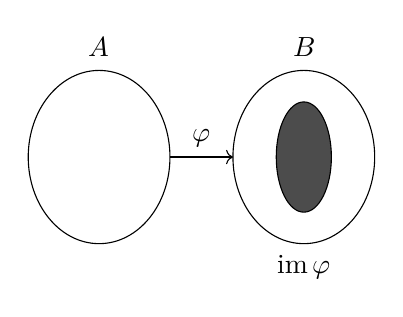
\begin{tikzpicture}[baseline=(current bounding box.center)]
    \draw (0,0) ellipse (0.9 and 1.1); \draw (2.6,0) ellipse (0.9 and
    1.1); \draw[fill=black!70] (2.6,0) ellipse (0.35 and 0.7);
    \draw[->] (0.9,0) -- (1.7,0) node[midway, above] {$\varphi$};
    \node at (0,1.4) {$A$}; \node at (2.6,1.4) {$B$}; \node at
    (2.6,-1.4) {$\image\varphi$};
  \end{tikzpicture}
\end{center}
We can fit many `subobjects' in $B$ to which $A$ maps via $\varphi$:
\begin{center}
  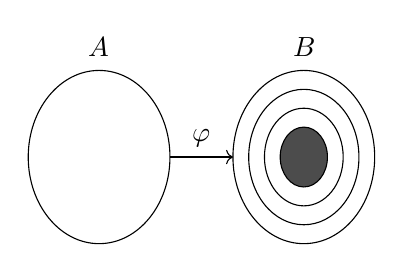
\begin{tikzpicture}[baseline=(current bounding box.center)]
    \draw (0,0) ellipse (0.9 and 1.1); \draw (2.6,0) ellipse (0.9 and
    1.1); \draw (2.6,0) ellipse (0.7 and 0.86); \draw (2.6,0) ellipse
    (0.5 and 0.62); \draw[fill=black!70] (2.6,0) ellipse (0.3 and
    0.38); \draw[->] (0.9,0) -- (1.7,0) node[midway, above]
    {$\varphi$}; \node at (0,1.4) {$A$}; \node at (2.6,1.4) {$B$};
  \end{tikzpicture}
\end{center}
and $\image\varphi$ is the `smallest' such subobject; that
is, it is initial with the property of being a subobject of $B$
through which $\varphi$ factors. This intuition is precisely captured
by $\ker(\coker\varphi)$, once we adapt to thinking of
`subobjects' as `monomorphisms':
\begin{lem}{}{homol:1.14}
  Let $\varphi : A \to B$ be a morphism in an abelian category, and
  let $\iota : K \to B$ be the kernel of the cokernel of $\varphi$.
  Then
  \begin{itemize}
  \item $\iota$ is a monomorphism;
  \item $\varphi$ factors through $\iota$; and
  \item $\iota$ is initial with these properties.
  \end{itemize}
\end{lem}

By Lemma~\ref{homol:1.4}, $\iota$ is a monomorphism. It is clear that
$\varphi$ factors through $\iota$: the composition
$A \to B \to \coker\varphi$ is the zero-morphism, so
there is a naturally induced $A \to K$ by the universal property of
kernels. The more interesting part of the statement of \Cref{homol:1.14}
asserts that if $\lambda : L \rightarrowtail B$ is any monomorphism
through which $\varphi$ also factors, then $\iota$ must factor
uniquely through $\lambda$:
\[\begin{tikzcd}
    & L \arrow[dr, hook, "\lambda"] & \\
    A \arrow[r] \arrow[rr, bend right, "\varphi"'] & K \arrow[u,
    dashed, "\exists!"] \arrow[r, hook, "\iota"'] & B
  \end{tikzcd}\]
\begin{proof}
  Consider $\coker\lambda$:
  \[\begin{tikzcd}
      & L \arrow[dr, "\lambda"] & \\
      A \arrow[ur] \arrow[r] & K \arrow[r, hook] &
      B \arrow[dr, "\coker\lambda"'] \\
      & & & \operatorname{Cok}\lambda
    \end{tikzcd}\] Since $\varphi$ factors through $\lambda$, the
  composition $A \to B \to \operatorname{Cok}\lambda$ is $0$; by the
  universal property of $\coker\varphi$, we have an
  induced map:
  \[\begin{tikzcd}
      & L \arrow[dr, "\lambda"] & & \\
      A \arrow[ur] \arrow[r] & K \arrow[r, hook] & B \arrow[r,
      "\coker\varphi"] \arrow[dr,
      "\coker\lambda"'] &
      \operatorname{Cok}_\varphi \arrow[d, dashed, "\exists!"] \\
      & & & \operatorname{Cok}\lambda
    \end{tikzcd}\] Since $K \to \operatorname{Cok}_\varphi$ is the
  zero-morphism, this implies that
  \[
    K \to B \xrightarrow{\coker\lambda}
    \operatorname{Cok}\lambda
  \]
  is the zero-morphism. Since $\lambda : L \to B$ is the kernel of its
  cokernel (Lemma~\ref{homol:1.8}), it follows that there is a unique
  morphism $K \to L$ making the diagram commute, as stated.
\end{proof}

\begin{defn}{}{homol:1.15}
  Let $\varphi : A \to B$ be a morphism in an abelian category. The
  \emph{image} of $\varphi$, denoted $\image\varphi$, is
  $\ker(\coker\varphi)$. The \emph{coimage} of
  $\varphi$, denoted $\operatorname{coim}\varphi$, is
  $\coker(\ker\varphi)$.
\end{defn}

Lemma~\ref{homol:1.14} motivates the first definition: every
monomorphism through which $\varphi$ factors must factor uniquely
through $\image\varphi$. (Of course in this context the
source of $\image\varphi$ is only defined up to (unique)
isomorphism, as is every solution to a universal problem.) As for the
second definition, the reader will formulate the universal property
satisfied by $\operatorname{coim}\varphi$ (\Cref{exer:homol:1.19}). With the
convention mentioned in \Cref{homol:1.7} and allowing for some abuse of
language, the (target of the) coimage of $\varphi : A \to B$ is the
`quotient' $A/\ker\varphi$.

My mental image, and surely yours, suggests that if $K \to B$ is the
image of $\varphi$, then the induced morphism
$\overline{\varphi} : A \to K$,
\[\begin{tikzcd}
    A \arrow[r, "\overline{\varphi}"] \arrow[rr, bend right,
    "\varphi"'] & K \arrow[r, hook] & B,
  \end{tikzcd}\] should be an epimorphism. This is indeed the case:
\begin{lem}{}{homol:1.16}
  Let $\varphi : A \to B$ be a morphism in an abelian category, and
  let $\image\varphi : K \to B$,
  $\operatorname{coim}\varphi : A \to C$ be its image and coimage,
  respectively. Then the induced morphisms $A \to K$ and $C \to B$
  are, respectively, an epimorphism and a monomorphism.
\end{lem}

\begin{proof}
  As usual, I will prove half of the statement and leave the other
  half to the reader (\Cref{exer:homol:1.20}.)

  To verify that $\overline{\varphi} : A \to K$ is an epimorphism,
  consider its image $K' \to K$:
  \[\begin{tikzcd}
      K' \arrow[r, hook, "\image\overline{\varphi} =
      \ker\coker\overline{\varphi}"] & K \arrow[r, two
      heads, "\coker\overline{\varphi}"] &
      \operatorname{Cok}.
    \end{tikzcd}\] Recall that every epimorphism is the cokernel of
  its kernel (Lemma~\ref{homol:1.8}); in particular,
  $\coker\overline{\varphi} =
  \coker(\image\overline{\varphi})$.  Now,
  $K' \to K$ is a monomorphism through which $\varphi$ factors:
  \[\begin{tikzcd}
      A \arrow[r] \arrow[rr, bend left, "\varphi"] & K' \arrow[r,
      hook, "\image\overline{\varphi}"] & K \arrow[r, hook]
      & B.
    \end{tikzcd}\] Therefore, $K' \to B$ is a monomorphism through
  which $\varphi$ factors and `preceding'
  $\image\varphi : K \to B$. Since the image of $\varphi$
  is initial among such morphisms (as proven in
  Lemma~\ref{homol:1.14}), necessarily
  $\image\overline{\varphi}$ is an isomorphism. It follows
  that
  $0 = \coker\image\overline{\varphi} =
  \coker\overline{\varphi}$, proving that
  $\overline{\varphi}$ is an epimorphism by Lemma~\ref{homol:1.5}.
\end{proof}
% ?
To summarize the situation, we have the following commutative diagram
of epimorphisms and monomorphisms factoring a given morphism $\varphi$
in an abelian category:
\[\begin{tikzcd}
    & K \arrow[dr, hook, "\image\varphi"] & \\
    A \arrow[ur, "\overline{\varphi}"] \arrow[rr, "\varphi"']
    \arrow[dr, two heads, "\operatorname{coim}\varphi"'] & & B. \\
    & C \arrow[ur, hook, "\underline{\varphi}"'] &
  \end{tikzcd}\]

Hopefully we have not lost track of our sought-for `canonical
decomposition':
\[
  \varphi : \quad
  \begin{tikzcd}
    A \arrow[r, two heads] & C \arrow[r, "\tilde{\varphi}", "\sim"'] &
    K \arrow[r, hook] & B.
  \end{tikzcd}
\]
We now see that this amounts to the statement that \emph{in an abelian
  category, there is an induced isomorphism linking the coimage and
  the image of every morphism.}

\begin{proof}[Proof of \cref{homol:1.13}]
  A unique morphism $\psi : K \to C$ making the above diagram commute
  exists, by the universal property of $\image\varphi$
  (Lemma~\ref{homol:1.14}), as well as by the universal property of
  $\operatorname{coim}\varphi$. Since
  $\underline{\varphi} \circ \psi = \image\varphi$ is a
  monomorphism, so is $\psi$. Since
  $\psi \circ \overline{\varphi} = \operatorname{coim}\varphi$ is an
  epimorphism, so is $\psi$. It follows that $\psi$ is an isomorphism
  (Lemma~\ref{homol:1.9}), and letting $\tilde{\varphi} : C \to K$ be
  the inverse of $\psi$ concludes the proof.
\end{proof}
Loosely speaking, we can say that, in an abelian category, `image and
coimage are naturally isomorphic'. This is imprecise, since image and
coimage are themselves morphisms; the isomorphism holds between the
target of coimage and the source of image. Of course, for friendly
categories such as $R\text{-}\categ{Mod}$ this distinction is
immaterial.

\subsection*{Exercises}

\begin{exer}{}{exer:homol:1.1}
  Prove that if $\psi \circ \varphi$ is an epimorphism, then $\psi$ is
  an epimorphism. Prove that if $\psi \circ \varphi$ is a
  monomorphism, then $\varphi$ is a monomorphism.
\end{exer}
\begin{exer}{}{exer:homol:1.2}
  Let $\varphi : A \to B$ be a morphism in an additive category. Prove
  that $-\varphi$ is a monomorphism, resp., epimorphism, if and only
  if $\varphi$ is.
\end{exer}
\begin{exer}{$\lnot$}{exer:homol:1.3}
  A \emph{preadditive} category is a category in which each Hom-set is
  endowed with an abelian group structure in such a way that
  composition maps are bilinear. Prove that a ring is `the same as' a
  preadditive category with a single object.

  Additive categories are preadditive categories with zero-objects and
  finite products and coproducts. Note that the notion of an `additive
  functor' between preadditive categories makes sense.  [\ref{exer:homol:1.12}]
\end{exer}
\begin{exer}{}{exer:homol:1.4}
  Let $\categ{A}$ be an additive category (preadditive would suffice),
  and let $A$ be an object of $\categ{A}$. Show that
  $\End_{\categ{A}}(A)$ has a natural ring structure.
\end{exer}
\begin{exer}{}{exer:homol:1.5}
  Let $A$, $B$ be objects of an additive category $\categ{A}$, with
  zero-object $0$. Since $0$ is both final and initial,
  $\Hom_{\categ{A}}(A,0)$ and $\Hom_{\categ{A}}(0,B)$ are both
  singletons, so the image of the composition
  \[
    A \to 0 \to B
  \]
  is a single element $e$ of $\Hom_{\categ{A}}(A,B)$.  Prove that this
  is the identity element of the abelian group
  $\Hom_{\categ{A}}(A,B)$. (Hint: Prove $e+e=e$.) In the text, this
  element is denoted $0$, the `zero-morphism'.

  Prove that for every morphism $\varphi$ in $\categ{A}$,
  $\varphi \circ 0 = 0 \circ \varphi = 0$.
\end{exer}
\begin{exer}{}{exer:homol:1.6}
  \exerused{} Prove that an object $A$ of an additive category
  $\categ{A}$ is a zero-object if and only if $\id_A$
  equals the zero-morphism $A \to A$. [\S{}\ref{subsec:homol:quasi-isomorphisms-and-derived-categories}]
\end{exer}
\begin{exer}{}{exer:homol:1.7}
  Give a categorical definition of cokernel in the spirit of the
  definition for kernel given in \Cref{linrep:exam:1.11}, and verify that
  the ordinary notion of cokernel in $R\text{-}\categ{Mod}$ satisfies
  this categorical requirement. Verify that your definition agrees
  with the one given in Definition~\ref{homol:1.2}.
\end{exer}
\begin{exer}{}{exer:homol:1.8}
  Let $\varphi : A \to B$ be a morphism in an additive category
  $\categ{A}$. Prove that $\iota : K \to A$ is a kernel for $\varphi$
  if and only if for all objects $Z$ the induced sequence
  \[\begin{tikzcd}
      0 \arrow[r] & \Hom_{\categ{A}}(Z,K) \arrow[r] &
      \Hom_{\categ{A}}(Z,A) \arrow[r] & \Hom_{\categ{A}}(Z,B)
    \end{tikzcd}\] is exact. Formulate an analogous result for
  cokernels.
\end{exer}
\begin{exer}{}{exer:homol:1.9}
  \exerused{} This exercise completes the proofs of results given in
  the text. The arguments should be constructed so as to mirror the
  proofs of the companion statements given in the quoted lemmas.

  Let $\categ{A}$ be an additive category.
  \begin{itemize}
  \item Let $\iota : K \to A$ be a kernel in $\categ{A}$; prove that
    $\iota$ is a monomorphism. (Cf.\ Lemma~\ref{homol:1.4}.)
  \item Let $\varphi : A \to B$ be a morphism in $\categ{A}$. If
    $\varphi$ has a cokernel, prove that $\varphi$ is an epimorphism
    if and only if $B \to 0$ is its cokernel. (Cf.\
    Lemma~\ref{homol:1.5}.)
  \item If $\categ{A}$ is abelian, prove that every kernel in
    $\categ{A}$ is the kernel of its cokernel. (Cf.\
    Lemma~\ref{homol:1.8}.)
  \end{itemize} [\S{}\ref{subsec:homol:abelian-categories}]
\end{exer}
\begin{exer}{}{exer:homol:1.10}
  \exerused{} Prove that the opposite $\categ{A}^{op}$ (cf.\
  \Cref{exer:3.1}) of an abelian category is an abelian category.
  [\S{}\ref{subsec:homol:complexes-of-projective-and-injective-objects}]
\end{exer}
\begin{exer}{$\lnot$}{exer:homol:1.11}
  Let $\categ{A}$ be an abelian category, and let $\categ{C}$ be any
  small category. Prove that the functor category
  $\categ{A}^{\categ{C}}$ (cf.\ \Cref{linrep:exer:1.9}) is an abelian
  category.

  For every object $X$ of $\categ{C}$, prove that the assignment
  $F \mapsto F(X)$ (with evident action on morphisms of
  $\categ{A}^{\categ{C}}$, i.e., natural transformations) determines
  an exact functor
  $\mathscr{X} : \categ{A}^{\categ{C}} \to \categ{A}$. [1.12, 1.14,
  1.15, 2.15, 5.7]
\end{exer}
\begin{exer}{}{exer:homol:1.12}
  For a ring $R$, let $\categ{R}$ denote the preadditive category with
  a single object determined by $R$ (\Cref{exer:homol:1.3}). Prove that the
  category $R\text{-}\categ{Mod}$ of left-$R$-modules is equivalent to
  the full subcategory consisting of additive functors in the functor
  category $\categ{Ab}^{\categ{R}}$ (cf.\ \Cref{exer:homol:1.11}). What about
  the category of right-$R$-modules?
\end{exer}
\begin{exer}{}{exer:homol:1.13}
  Let $R$ be a commutative ring, and let $R\text{-}\categ{Mod}^f$
  denote the category of finitely generated $R$-modules. Show that
  $R\text{-}\categ{Mod}^f$ need not be an abelian category; prove that
  it is, provided $R$ is Noetherian.
\end{exer}
\begin{exer}{}{exer:homol:1.14}
  Let $T$ be a topological space. Recall that a presheaf on $T$ with
  values in a category $\categ{A}$ is a contravariant functor from a
  certain category associated with $T$ to $\categ{A}$
  (\Cref{linrep:exam:1.5}). Define the \emph{category} of $\categ{A}$-valued
  presheaves on $T$. Prove that presheaves on $T$ with values in an
  abelian category form an abelian category. (Hint: \Cref{exer:homol:1.11}.)
\end{exer}
\begin{exer}{}{exer:homol:1.15}
  Consider the presheaf of continuous complex-valued functions
  $\mathscr{C}$ on a circle $S^1$ (cf.\ \Cref{linrep:exer:1.6}) and the
  presheaf $\mathscr{C}^*$ of continuous complex-valued functions that
  do not vanish anywhere along the circle; the first is a sheaf of
  abelian groups (under $+$), and so is the second (under $\cdot$).
  Use the exponential map to define a morphism
  $\exp : \mathscr{C} \to \mathscr{C}^*$.

  Prove that $\exp$ is \emph{not} an epimorphism of
  presheaves\footnote{Watch out! Both presheaves $\mathscr{C}$,
    $\mathscr{C}^*$ satisfy the \emph{sheaf} condition; cf.\
    \Cref{linrep:exer:1.6}. Sheaves of abelian groups form a full
    subcategory of the category of presheaves, and this category is
    also abelian, but the inclusion functor is in general \emph{not}
    exact. For example, the exponential map
    $\mathscr{C} \to \mathscr{C}^*$ considered above \emph{is} an
    epimorphism of sheaves.

    Also, for every open set $U$ of $T$, the assignment
    $F \mapsto F(U)$ defines a functor both on the category of
    presheaves of abelian groups and on the category of sheaves of
    abelian groups. This functor is exact on presheaves (this is a
    particular case of \Cref{exer:homol:1.11}), but the example given above
    shows that it is not exact in general on sheaves. This lack of
    exactness is responsible for the existence of sheaf cohomology.}:
  show that its cokernel has value $0$ over every proper open set of
  $S^1$ but is nonzero over $S^1$.
\end{exer}
\begin{exer}{}{exer:homol:1.16}
  \exerused{} Consider the pull-back diagram
  \[\begin{tikzcd}
      A \times_C B \arrow[r, "\varphi'"] \arrow[d, "\psi'"']
      \arrow[dr, phantom, "\lrcorner", very near start] &
      B \arrow[d, "\psi"] \\
      A \arrow[r, "\varphi"'] & C
    \end{tikzcd}\] in an abelian category; prove that the induced
  morphism from the source of $\ker\varphi'$ to the source of
  $\ker\varphi$ is an isomorphism.

  State and prove an analogous result for push-outs. [\S{}1.4,
  \S{}2.2, \S{}6.2]
\end{exer}
\begin{exer}{}{exer:homol:1.17}
  \exerused{} Prove that the morphism $A \amalg B \to A \times B$
  defined for objects $A$, $B$ of an abelian category is an
  epimorphism. [\S{}\ref{subsec:homol:products-coproducts-and-direct-sums}]
\end{exer}
\begin{exer}{}{exer:homol:1.18}
  Formulate a notion of `intersection' of two monomorphisms with a
  common target $A \rightarrowtail Z$, $B \rightarrowtail Z$ in an
  abelian category. Prove that the intersection of the natural
  monomorphisms $A \rightarrowtail A \oplus B$,
  $B \rightarrowtail A \oplus B$ is $0$.
\end{exer}
\begin{exer}{}{exer:homol:1.19}
  \exerused{} Formulate the universal property satisfied by the
  coimage of a morphism in an abelian category. [\S{}\ref{subsec:homol:images-canonical-decomposition-of-morphisms}]
\end{exer}
\begin{exer}{}{exer:homol:1.20}
  \exerused{} Let $A \to B$ be a morphism in an abelian category, with
  coimage $A \to C$, and let $C \to B$ be the induced morphism. Prove
  that $C \to B$ is a monomorphism. (Cf.\ Lemma~\ref{homol:1.16}; you
  should not use Theorem~\ref{homol:1.13}, since
  Lemma~\ref{homol:1.16} was used in its proof.) [\S{}\ref{subsec:homol:images-canonical-decomposition-of-morphisms}]
\end{exer}
\begin{exer}{$\lnot$}{exer:homol:1.21}
  Let $\varphi : A \to B$ be a morphism in an abelian category, and
  assume $\varphi$ decomposes as an epimorphism $\pi$ followed by a
  monomorphism $i$:
  \[\begin{tikzcd}
      A \arrow[r, two heads, "\pi"'] \arrow[rr, bend left, "\varphi"]
      & C \arrow[r, hook, "i"'] & B.
    \end{tikzcd}\] Prove that necessarily
  $\pi = \operatorname{coim}\varphi$ and
  $i = \image\varphi$. [\S{}\ref{subsec:homol:long-exact-sequence-of-derived-functors}]
\end{exer}
\begin{exer}{}{exer:homol:1.22}
  \exerused{} Prove that finite products and coproducts coincide in
  any \emph{additive} category. (Hint: To show that $A \amalg B$
  satisfies the universal property for $A \times B$, let
  $\alpha : C \to A$ and $\beta : C \to B$ be two morphisms, and
  define $C \to A \amalg B$ by $i_A \circ \alpha + i_B \circ \beta$.)
  [\S{}\ref{subsec:homol:products-coproducts-and-direct-sums}]
\end{exer}

\section{Working in abelian categories}
\label{sec:homol:working-in-abelian-categories}


\subsection{Exactness in abelian categories}
\label{subsec:homol:exactness-in-abelian-categories}
Now that we have a good notion of image in any abelian category, we
can formalize the meaning of `exact sequence'. Consider a sequence of
objects and morphisms in an abelian category:
\[\begin{tikzcd}
    \dots \arrow[r] & A \arrow[r, "\varphi"] & B \arrow[r, "\psi"] & C
    \arrow[r] & \dots.
  \end{tikzcd}\] The sequence is \emph{exact at $B$} if
\begin{enumerate}[label=(\arabic*)]
\item $\psi \circ \varphi = 0$ and
\item $\coker\varphi \circ \ker\psi = 0$.
\end{enumerate}
The first condition makes the sequence a `complex'; it tells us that
$\varphi$ factors through $\ker\psi$. As $\ker\psi$ is a monomorphism,
the universal property of images (Lemma~\ref{homol:1.14}) yields a
unique factorization of $\image\varphi$ through $\ker\psi$.
Similarly, the second condition tells us that $\ker\psi$ factors
through
$\ker(\coker\varphi) = \image\varphi$.  This
implies that $\image\varphi$ and $\ker\psi$ coincide.  The
conditions defining exactness can therefore be summarized as
\begin{itemize}
\item $\image\varphi = \ker\psi$.
\end{itemize}
Of course this recovers precisely the condition used to define the
notion of exactness of a sequence of $R$-modules, in \ref{subsec:rings:complexes-and-exact-sequences}. All
expected elementary connotations of exactness hold in the context of
abelian categories as in $R\text{-}\categ{Mod}$, as envisioned already
in \S{}1.2--1.3. With notation as above, if the sequence is exact at
$B$, then $\psi$ is a monomorphism if and only if $\varphi$ is the
zero-morphism, and $\varphi$ is an epimorphism if and only if $\psi$
is the zero-morphism; the sequence
\[\begin{tikzcd}
    0 \arrow[r] & A \arrow[r, "\varphi"] & B \arrow[r, "\psi"] & C
    \arrow[r] & 0
  \end{tikzcd}\] is exact if and only if $\varphi$ is a kernel of
$\psi$ and $\psi$ is a cokernel of $\varphi$, and
\[\begin{tikzcd}
    0 \arrow[r] & A \arrow[r, "\varphi"] & B \arrow[r] & 0
  \end{tikzcd}\] is exact if and only if $\varphi$ is an isomorphism.
\begin{exam}{}{homol:2.1}
  There is a natural exact sequence
  \[\begin{tikzcd}
      0 \arrow[r] & A \arrow[r] & A \oplus B \arrow[r] & B \arrow[r] &
      0
    \end{tikzcd}\] where $A \oplus B$ is the direct sum defined in
  \S{}1.4.
\end{exam}
\begin{exam}{}{homol:2.2}
  For a slightly more interesting example, consider a diagram
  \[\begin{tikzcd}
      D \arrow[r, "\varphi'"] \arrow[d, "\psi'"'] & B \arrow[d, "\psi"] \\
      A \arrow[r, "\varphi"'] & C
    \end{tikzcd}\] and the associated sequence
  \[\begin{tikzcd}
      D \arrow[r, "{(\psi', \varphi')}"] & A \oplus B \arrow[r,
      "{(\varphi, -\psi)}"] & C
    \end{tikzcd}\] obtained by letting $A \oplus B$ play both roles of
  product and coproduct. Then
  \begin{itemize}
  \item the diagram is commutative if and only if this sequence is a
    complex;
  \item the sequence obtained by adding a $0$ to the left,
    \[\begin{tikzcd}
        0 \arrow[r] & D \arrow[r] & A \oplus B \arrow[r] & C,
      \end{tikzcd}\] is exact if and only if $D$ may be identified
    with the fibered product $A \times_C B$ (cf.\
    Example~\ref{homol:exam:1.11});
  \item likewise, the sequence
    \[\begin{tikzcd}
        D \arrow[r] & A \oplus B \arrow[r] & C \arrow[r] & 0
      \end{tikzcd}\] is exact if and only if $C$ may be identified
    with the fibered coproduct $A \amalg_D B$.
  \end{itemize}
  Indeed, the first assertion is trivial; the second and third amount
  to the explicit construction of fibered products and coproducts
  mentioned in Example~\ref{homol:exam:1.11}.
\end{exam}

\subsection{The snake lemma, again}
\label{subsec:homol:the-snake-lemma-again}
The reader is now in the position of making sense in any abelian
category of all the statements given in \ref{sec:rings:complexes-and-homology} for sequences of
$R$-modules; this includes the definition of the \emph{homology} of a
complex as a measure of the failure of exactness. These facts will be
reviewed in \S{}3. However, note that while we can now \emph{state}
the snake lemma (\Cref{lem:rings:snake-lemma}) in any abelian category, the (sketch
of the) \emph{proof} given in \ref{sec:rings:complexes-and-homology} cannot be directly lifted from
that context and applied to this one, or so it would seem, since the
definition of the `snaking' homomorphism $\delta$ given in \ref{sec:rings:complexes-and-homology}
makes use of `elements'. Barring more sophisticated alternatives, we
should provide an arrow-theoretic alternative for the definition of
$\delta$.

This is perhaps not completely immediate.

As practice, note the following:
\begin{lem}{}{homol:2.3}
  Let
  \[\begin{tikzcd}
      A \times_C B \arrow[r, "\varphi'"] \arrow[d, "\psi'"'] &
      B \arrow[d, "\psi"] \\
      A \arrow[r, "\varphi"'] & C
    \end{tikzcd}\] be a fibered diagram in an abelian category, and
  assume $\varphi$ is an epimorphism. Then $\varphi'$ is also an
  epimorphism.
\end{lem}

It takes seconds to realize that this is true in
$R\text{-}\categ{Mod}$, by chasing elements. An arrow-theoretic proof
is considerably subtler.

\begin{proof}
  First, observe that if $\varphi : A \to C$ is an epimorphism, so is
  the map $A \oplus B \to C$ considered in Example~\ref{homol:2.2}.
  Since epimorphisms are cokernels in an abelian category and
  cokernels are cokernels of their kernels (Lemma~\ref{homol:1.8}), we
  see that $A \oplus B \to C$ is the cokernel of the natural morphism
  \[
    A \times_C B \to A \oplus B.
  \]
  To prove that $\varphi'$ is an epimorphism, it suffices
  (Lemma~\ref{homol:1.3}) to show that if $\zeta : B \to Z$ is a
  morphism for which $\zeta \circ \varphi' = 0$, then $\zeta = 0$.

  For this, consider the morphism
  \[\begin{tikzcd}
      A \oplus B \arrow[r, "{(0,\zeta)}"] & Z
    \end{tikzcd}\] obtained by using the fact that $A \oplus B$ is a
  coproduct of $A$ and $B$. The composition
  \[
    A \times_C B \to A \oplus B \to Z
  \]
  agrees with $\zeta \circ \varphi'$, so it is the zero-morphism. By
  the universal property of cokernels, we have the factorization
  \[\begin{tikzcd}
      A \oplus B \arrow[r, "{(0,\zeta)}"] \arrow[d] & Z \\
      C \arrow[ur, dashed, "\zeta'"']
    \end{tikzcd}\] for a unique morphism $\zeta'$. By the
  commutativity of
  \[\begin{tikzcd}
      A \arrow[r] \arrow[dr, "\varphi"'] &
      A \oplus B \arrow[r, "{(0,\zeta)}"] & Z \\
      & C \arrow[ur, "\zeta'"'] &
    \end{tikzcd}\] we see that the composition
  $\zeta' \circ \varphi : A \to C \to Z$ is the zero-morphism. Since
  $\varphi$ is an epimorphism, it follows that $\zeta' = 0$. This
  implies that $(0,\zeta) : A \oplus B \to Z$ is the zero-morphism,
  and we are done: $\zeta = 0$ as promised.
\end{proof}

Here is a quicker proof (for those who have done their homework): if
$\varphi$ is an epimorphism, then $A \oplus B \to C$ is an
epimorphism, so the diagram is a push-out as well as a pull-back
(Example~\ref{homol:2.2}). By \Cref{exer:homol:1.16},
$\coker\varphi' = \coker\varphi = 0$;
therefore $\varphi'$ is an epimorphism. The reader should have no
difficulty now proving the statement dual to Lemma~\ref{homol:2.3},
for fibered coproducts (\Cref{exer:homol:2.2}).  Going back to the snake lemma,
start from a commutative diagram linking two exact sequences in an
abelian category:
\[\begin{tikzcd}
    0 \arrow[r] & L_1 \arrow[r, "\alpha_1"] \arrow[d, "\lambda"'] &
    M_1 \arrow[r, "\beta_1"] \arrow[d, "\mu"'] &
    N_1 \arrow[r] \arrow[d, "\nu"'] & 0 \\
    0 \arrow[r] & L_0 \arrow[r, "\alpha_0"'] & M_0 \arrow[r,
    "\beta_0"'] & N_0 \arrow[r] & 0
  \end{tikzcd}\] The main task is to construct a connecting
morphism\footnote{To avoid unbearably heavy notation, I will write
  $\ker\nu$, etc., for the \emph{source} of the morphism $\ker\nu$,
  etc.}  $\delta : \ker\nu \to \coker\lambda$; once this
is done, we should prove the exactness of the sequence displayed in
\Cref{lem:rings:snake-lemma}. I will leave this latter step to the more enterprising
reader (who may want to wait until we go through \S{}2.3).  The
enterprising reader should in fact try to construct $\delta$, as an
exercise in coming up with arrow-theoretic proofs replacing
well-understood element-theoretic arguments. Feel free to stop reading
here and resume when you have tried on your own.

The `problem' is that the universal properties of kernel and cokernel
would seem to guarantee the existence of morphisms \emph{to} $\ker\nu$
and \emph{from} $\coker\lambda$. There's the rub: how on
earth are we going to get a morphism \emph{from} $\ker\nu$ \emph{to}
$\coker\lambda$? (Last chance to try on your own!)

The answer is to view $\ker\nu$ as a cokernel and
$\coker\lambda$ as a kernel. This can be achieved by
constructing suitable pull-back, resp., push-out, diagrams:
\[\begin{tikzcd}
    M_1 \times_{N_1} (\ker\nu) \arrow[r, "\beta_1'"] \arrow[d] &
    \ker\nu \arrow[d] \\
    M_1 \arrow[r, "\beta_1"'] & N_1
  \end{tikzcd}\!, \qquad
  \begin{tikzcd}
    L_0 \arrow[r, "\alpha_0"] \arrow[d] & M_0 \arrow[d] \\
    \coker\lambda \arrow[r, "\alpha_0'"'] &
    (\coker\lambda) \amalg_{L_0} M_0.
  \end{tikzcd}\] By Lemma~\ref{homol:2.3}, $\beta_1'$ is an
epimorphism since $\beta_1$ is an epimorphism, and $\ker\beta_1$,
$\ker\beta_1'$ have matching sources by \Cref{exer:homol:1.16}. Analogous
(dual) statements hold for the second diagram (Exercises~2.2 and
1.16). Putting everything into one commutative diagram,
\[\begin{tikzcd}[column sep=small]
    0 \arrow[r] & L_1 \arrow[r, "\sigma"] \arrow[d, equal] & M_1
    \times_{N_1} (\ker\nu) \arrow[r, "\beta_1'"] \arrow[ddd,
    "\epsilon", bend left=25] &
    \ker\nu \arrow[r] \arrow[d] & 0 \\
    0 \arrow[r] & L_1 \arrow[r, "\alpha_1"'] \arrow[d, "\lambda"'] &
    M_1 \arrow[r, "\beta_1"'] \arrow[d, "\mu"'] &
    N_1 \arrow[r] \arrow[d, "\nu"'] & 0 \\
    0 \arrow[r] & L_0 \arrow[r, "\alpha_0"'] \arrow[d] & M_0 \arrow[r,
    "\beta_0"'] \arrow[d] &
    N_0 \arrow[r] \arrow[d, equal] & 0 \\
    0 \arrow[r] & \coker\lambda \arrow[r, "\alpha_0'"']
    & (\coker\lambda) \amalg_{L_0} M_0 \arrow[r,
    "\tau"'] & N_0 \arrow[r] & 0
  \end{tikzcd}\] has exact rows (not columns!). We get a morphism
\[
  \epsilon : M_1 \times_{N_1} (\ker\nu) \to
  (\coker\lambda) \amalg_{L_0} M_0.
\]
Note that
\[
  \epsilon \circ \sigma = 0, \qquad \tau \circ \epsilon = 0
\]
by the commutativity of the diagram: indeed, the compositions
$L_1 \to \coker\lambda$, $\ker\nu \to N_0$ are both
zero.  Since $\ker\nu$ plays the role of cokernel in the top row,
$\epsilon \circ \sigma = 0$ implies that $\epsilon$ must factor
through $\ker\nu$, giving a morphism
\[
  \epsilon' : \ker\nu \to (\coker\lambda) \amalg_{L_0}
  M_0.
\]
Since $\coker\lambda$ plays the role of kernel in the
bottom row and $\tau \circ \epsilon' : \ker\nu \to N_0$ is the
zero-morphism (because
$\tau \circ \epsilon' \circ \beta_1' = \tau \circ \epsilon = 0$ and
$\beta_1'$ is an epimorphism), $\epsilon'$ must factor through
$\coker\lambda$, finally yielding
\[
  \delta : \ker\nu \to \coker\lambda.
\]
Writing elements out, the reader can verify that this morphism
$\delta$ agrees with the connecting morphism $\delta$ defined in
\ref{subsec:rings:homology-and-the-snake-lemma}. Together with maps induced by simpler considerations, we
obtain the sequence of morphisms
\[\begin{tikzcd}[column sep=small]
    0 \arrow[r] & \ker\lambda \arrow[r] & \ker\mu \arrow[r] & \ker\nu
    \arrow[r, "\delta"] & \coker\lambda \arrow[r] &
    \coker\mu \arrow[r] & \coker\nu
    \arrow[r] & 0
  \end{tikzcd}\] in our abelian category. I should now recommend that
the reader prove the exactness of this sequence, by appropriate
arrow-theoretic arguments. This would be excellent practice for many
such facts that we will encounter when we finally do begin to develop
homological algebra.

However, assuming that we have already done this work in \ref{subsec:rings:homology-and-the-snake-lemma},
by chasing elements, is it really necessary to go back and redo it
with arrows, in order to check the exactness of the sequence in an
abelian category?

\subsection{Working with `elements' in a small abelian category}
\label{subsec:homol:working-with-elements-in-a-small-abelian-category}
My personal feeling is that arrow-theoretic arguments are invariably
more insightful than their element-theoretic counterparts, even if
they are `harder' as a rule. At the very least, they are more elegant:
for example, in the construction of the connecting morphism $\delta$
just given above, there was no need to verify that the result was
`well-defined', while this requires an argument in the set-theoretic
construction in \ref{subsec:rings:homology-and-the-snake-lemma}. Such issues are usually resolved once and
for all at the start, when the key universal properties are
established, and it is not necessary to belabor them later.  Still, it
is true that element-theoretic arguments are usually easier to
concoct. Lemma~\ref{homol:2.3} appears to be a good example: in terms
of elements the statement of this lemma is completely obvious, less so
from the diagrammatic point of view. \Cref{exer:homol:2.12} gives another
example: providing a purely arrow-theoretic proof of the innocent
result stated there is not so easy, while this result is essentially
immediate from a more mundane viewpoint. The reader could wonder
whether it may not `be enough' to prove such facts---for example,
check the commutativity of a diagram or the exactness of a
sequence---by simpler element-theoretic considerations.  This is
indeed the case. I will present a construction which would suffice
for, e.g., the purpose of completing the proof of the snake lemma by
chasing elements rather than arrows. I find this construction
instructive and pretty, so I will take the time to go through it in
some detail. However, be warned that the Freyd--Mitchell embedding
theorem (discussed in \S{}2.4) will obliterate the actual usefulness
of the construction, since it provides us with a much stronger result.
Thus, I will ask the reader to wade through some material, with the
understanding that the result that I will quote thereafter
(\Cref{homol:2.9}) will make that material immediately obsolete.

My excuse is that while proving \Cref{homol:2.9} is beyond the scope of
this book, the construction which I am about to describe is entirely
within our reach, and good propaganda for the philosophy underlying
the functor of points; this is important in, e.g., algebraic geometry
and takes some practice to get used to. In the end, the reader is
likely to gain a better understanding of the situation by appreciating
a weaker result that we can prove entirely than by leaning on a
stronger result to be taken on faith. However, the hurried reader
should feel free to skip this material and jump directly to \S{}2.4.
The idea is to define an appropriate notion of an `element' of an
object of an abelian category.\footnote{I will systematically put
  quotes around this term, i.e., write `element', to indicate that I
  am referring to the relatively fancy notion I will introduce. The
  `elements' will be ordinary elements of an ordinary (pointed) set
  determined by the object of the category.} The reader should look
back at the brief discussion at the end of \ref{subsec:linrep:examples-of-functors}: the `functor
of points' $h_A = \Hom_{\categ{A}}(\_, A)$ associates to every object
$Z$ the set of morphisms $Z \to A$; in several categories, applying
this functor to a final object in $\categ{A}$ `recovers' $A$ as a
set. Working with final objects with this purpose cannot work too well
in categories with zero-objects (why?), but the idea underlying the
functor of points suggests that we look at morphisms
\[
  z : Z \to A
\]
for a fixed object $A$ in an abelian category $\categ{A}$ as
($Z$-flavored?!) `elements' $z$ of $A$.

If $\varphi : A \to B$ is a morphism in $\categ{A}$, it makes sense to
talk about the `element' $\varphi(z)$ of $B$: simply compose
morphisms, i.e.,
\[\begin{tikzcd}
    & Z \arrow[d, "z"'] \arrow[dr, "\varphi(z) = \varphi \circ z"] & \\
    & A \arrow[r, "\varphi"'] & B
  \end{tikzcd}\]

It would now be nice if one could simply check the commutativity of a
diagram in $\categ{A}$ or the exactness of a sequence by using these
newly defined `elements' as if they were elements of objects in
$\categ{A}$. This does not quite work: for example, the simple-minded
statement of surjectivity at the level of these `elements' is not
equivalent to the notion of epimorphism in $\categ{A}$. Indeed, if
$\varphi : A \to B$ is an epimorphism, it is not necessarily the case
that `for all elements $z$ of $B$ there exists an element $z'$ of $A$
such that $z = \varphi(z')$': this would amount to saying that every
morphism $z : Z \to B$ can be lifted to a morphism $z' : Z \to A$,
\[\begin{tikzcd}
    & A \arrow[d, "\varphi"] \\
    Z \arrow[ur, dashed, "\exists z'?"] \arrow[r, "z"'] & B
  \end{tikzcd}\] and this is simply not true in general (for example,
in $\categ{Ab}$ one cannot lift the identity $\Z/2\Z \to \Z/2\Z$ along
the projection $\Z \to \Z/2\Z$). The problem is really that $\Hom$ is
not right-exact, so it does not preserve epimorphisms.

Maybe surprisingly, there is a way to fix this problem.  As a
preliminary note, recall that in the distant past (\Cref{exam:prelims:pointed-sets}) we
considered the category $\categ{Set}^*$ of `pointed sets', whose
objects consist of sets endowed with the choice of a distinguished
point (here I will denote by $0$ the distinguished point). All the
algebraic structures we have encountered are pointed sets, often in
more than one way: for example, stripping an abelian group of all its
structure except its supporting set and the choice of the identity
element leaves us with a pointed set (in other words, this defines an
evident forgetful functor $\categ{Ab} \to \categ{Set}^*$).

The category $\categ{Set}^*$ has a zero-object $0$ (the singleton
$\{0\}$); hence we can talk of `zero-morphisms' in $\categ{Set}^*$.
Further, the category $\categ{Set}^*$ has enough structure to make
sense of the notion of an `exact sequence of pointed sets': we can
stipulate that
\[\begin{tikzcd}
    \dots \arrow[r] & S \arrow[r, "f"] & T \arrow[r, "g"] & U
    \arrow[r] & \dots
  \end{tikzcd}\] is `exact' at $T$ if the (set-theoretic!) image of
$f$ equals the `kernel' of $g$ (that is, the preimage
$g^{-1}(0)$). This notion should be taken with a grain of salt: while
it is the case that $S \to T \to 0$ is exact at $T$ if and only if
$S \to T$ is surjective, it is not true that $0 \to T \to U$ is exact
at $T$ in $\categ{Set}^*$ if and only if $T \to U$ is injective (the
only requirement posed by the exactness of $0 \to T \to U$ is that the
only element of $T$ mapping to the distinguished element in $U$ is the
distinguished element of $T$; this is weaker than injectivity). The
category $\categ{Set}^*$ is, after all, not additive.  Now we are
going to associate to every object $A$ of a (small) abelian category
$\categ{A}$ a pointed set $\hat{A}$. This will in fact give a functor
$\categ{A} \to \categ{Set}^*$ with amazing properties: a morphism will
be a monomorphism, resp., an epimorphism, in $\categ{A}$ if and only
if the corresponding function of pointed sets is injective, resp.,
surjective; the (arrow-theoretic) notions of kernel and image in
$\categ{A}$ will correspond precisely to the (set-theoretic) kernel
and image in $\categ{Set}^*$; a sequence of objects in $\categ{A}$
will be exact if and only if the corresponding sequence of pointed
sets is exact; and it will be possible to verify whether a diagram
commutes in $\categ{A}$ by working in $\categ{Set}^*$.

The upshot will be that in a sense we can chase a diagram in any small
abelian category by `chasing elements'. For example, working with
`elements' suffices to complete the proof of the snake lemma, in the
sense that the exactness (in $\categ{A}$) of the sequence obtained
with the aid of the connecting morphism defined in \S{}2.2 may be
verified by chasing `elements', since this verifies exactness in
$\categ{Set}^*$. A proof in $R\text{-}\categ{Mod}$ would transfer
word-for-word to give a proof in any small\footnote{If the relevant
  diagrams only involve finitely many objects, the smallness
  hypothesis is not restrictive. The interested reader should research
  this issue; I will shamelessly gloss over it.} abelian
category. This hints that the arrow-theoretic viewpoint that I have
tried to defend in the past several subsections, while elegant, is not
really strictly necessary; I will come back to this point in \S{}2.4.
The construction can be given as an application of the abstract
language developed in \ref{sec:linrep:preliminaries-reprise}; but I promise that the resulting
notion will be easy to contemplate, independently of this language.
The idea is simply to take the functor of points up to a relation
identifying the `element' $Z \to A$ with all `elements'
$W \twoheadrightarrow Z \to A$.

The following abstract nonsense will have a simple-minded explanation.
I will (often silently) assume that $\categ{A}$ is small, to steer
clear of any possible set-theoretic subtlety. It is convenient to
consider a companion category $\categ{A}_{\leftarrow}$, with the same
objects as $\categ{A}$ but in which
\[
  \Hom_{\categ{A}_{\leftarrow}}(Z,W) = \{\text{epimorphisms } W
  \twoheadrightarrow Z \text{ in } \categ{A}\}.
\]
This is legal, because the composition of two epimorphisms in
$\categ{A}$ is an epimorphism; but note that $\categ{A}_{\leftarrow}$
is no longer additive (the sum of two epimorphisms need not be an
epimorphism, so we lose the algebraic structure on Hom). Also note the
reversing of arrows; this is in order that the functor that I am about
to define be covariant.

I will use $\categ{A}_{\leftarrow}$ as `index' category for a limit.
For a fixed object $A$ of $\categ{A}$, I define a covariant functor
\[
  \mathscr{H}_A : \categ{A}_{\leftarrow} \to \categ{Set}^*
\]
by `restricting' the functor of points $h_A$ to
$\categ{A}_{\leftarrow}$ and preserving the information of the
zero-morphism. That is, I set
\[
  \mathscr{H}_A(Z) = \Hom_{\categ{A}}(Z,A)
\]
for all objects $Z$ of $\categ{A}_{\leftarrow}$ (that is, of
$\categ{A}$), viewing $\Hom_{\categ{A}}(Z,A)$ as a pointed set by
distinguishing the zero-morphism, and define $\mathscr{H}_A$ on
morphisms by composition: for a morphism $Z \to W$ in
$\categ{A}_{\leftarrow}$ (that is, an epimorphism
$\alpha : W \twoheadrightarrow Z$),
\[\begin{tikzcd}
    W \arrow[rr, "\alpha"] \arrow[dr, "w"'] & & Z \arrow[dl, "z"] \\
    & A &
  \end{tikzcd}\] define
\[
  \mathscr{H}_A(Z) \to \mathscr{H}_A(W)
\]
by sending $z$ to $w = z \circ \alpha$. Of course the zero-morphism is
mapped to the zero-morphism, so this is indeed a morphism in
$\categ{Set}^*$.
\begin{defn}{}{homol:2.4}
  Let $A$ be an object of a small abelian category $\categ{A}$. The
  pointed set $\hat{A}$ of `elements of $A$' is the colimit of
  $\mathscr{H}_A$:
  \[
    \hat{A} := \varinjlim \mathscr{H}_A.
  \]
\end{defn}

Here is the simple-minded explanation. In the context of pointed sets,
colimits may be constructed by joining pointed sets at the
distinguished point and then taking a suitable quotient. For the case
at hand, this translates into the following: an `element' of $A$
consists of the choice of a morphism $z : Z \to A$ in $\categ{A}$,
stipulating that two morphisms $z_1 : Z_1 \to A$, $z_2 : Z_2 \to A$
determine the same `element' if there are epimorphisms
$w_1 : W \twoheadrightarrow Z_1$ and $w_2 : W \twoheadrightarrow Z_2$
in $\categ{A}$ such that the diagram
\[\begin{tikzcd}
    & Z_1 \arrow[dr, "z_1"] & \\
    W \arrow[ur, "w_1", two heads] \arrow[dr, "w_2"', two heads] & & A \\
    & Z_2 \arrow[ur, "z_2"'] &
  \end{tikzcd}\] commutes. This is an equivalence relation, as the
reader should check carefully (\Cref{exer:homol:2.5}).  Now I want to make the
assignment $A \mapsto \hat{A}$ into a covariant functor
$\categ{A} \to \categ{Set}^*$, and there is only one reasonable way to
do so: for $\varphi : A \to B$ and $z : Z \to A$, define
$\hat{\varphi}(z)$ by composing morphisms, i.e.,
\[\begin{tikzcd}
    & A \arrow[d, "\varphi"] \\
    Z \arrow[ur, "z"] \arrow[r, "\hat{\varphi}(z) := \varphi \circ
    z"'] & B
  \end{tikzcd}\] This prescription is (manifestly) compatible with the
equivalence relation, so it defines a set-function
$\hat{\varphi} : \hat{A} \to \hat{B}$. The image of the zero-morphism
is zero, so $\hat{\varphi}$ is a morphism in $\categ{Set}^*$, as
needed. The covariance property of this assignment is evident. We have
obtained the promised functor $\categ{A} \to \categ{Set}^*$.

Now we will proceed to verify all the miracles I have advertised. In
the following, the symbol $\sim$ will stand for the equivalence
relation defined above\footnote{Warning: Later on in this chapter I
  will define a notion of homotopy, and I will recycle the symbol
  $\sim$ for that notion. The context and the meaning of the symbol
  will be completely different.}; thus, two morphisms
$z_1 : Z_1 \to A$, $z_2 : Z_2 \to A$ determine the same `element' of
$\hat{A}$ if and only if $z_1 \sim z_2$.

One useful preliminary observation is that the only morphism
representing the distinguished `element' is the zero-morphism and that
we can detect whether a morphism is $0$ by working in $\categ{Set}^*$:
\begin{lem}{}{homol:2.5}
  $z \sim 0 \iff z = 0$. Further, a morphism $\varphi : A \to B$ in
  $\categ{A}$ is $0$ if and only if $\hat{\varphi}(z) = 0$ for all
  $z \in \hat{A}$.
\end{lem}

\begin{proof}
  According to the definition given above, $z : Z \to A$ is equivalent
  to $0$ if and only if there is an epimorphism
  $W \twoheadrightarrow Z$ making the following diagram commute:
  \[\begin{tikzcd}
      W \arrow[r, two heads] & Z \arrow[r, "z"] & A
    \end{tikzcd}\] Since $W \twoheadrightarrow Z$ is an epimorphism,
  this diagram commutes if and only if $z = 0$
  (Lemma~\ref{homol:1.3}), as claimed.

  For the second statement, consider the situation
  \[\begin{tikzcd}
      A \arrow[r, "\varphi"] & B \\
      Z \arrow[u, "z"] \arrow[ur, dashed, "\hat{\varphi}(z)"'] &
    \end{tikzcd}\] If $\varphi = 0$, then so is
  $\hat{\varphi}(z) = \varphi \circ z$.  Conversely, if
  $\hat{\varphi}(z) = 0$ for all $z$, then taking $z : Z = A \to A$ to
  be the identity, we get $\varphi \sim 0$, and hence $\varphi = 0$ by
  the first part.
\end{proof}
This tells us in particular that we can verify the commutativity of a
diagram in $\categ{A}$ by working in $\categ{Set}^*$: because we can
check whether two morphisms $\varphi, \psi \in \Hom_{\categ{A}}(A,B)$
are equal by verifying that their difference $\varphi - \psi$ equals
$0$, which we can do\footnote{Note that I am not saying that
  $\varphi = \psi$ if and only if $\hat{\varphi}(z) = \hat{\psi}(z)$
  for all `elements' $z$; this is unfortunately not the case (cf.\
  \Cref{exer:homol:2.10}).} at the level of pointed sets (hence, by chasing
elements!) by Lemma~\ref{homol:2.5}.

Concerning monomorphisms and epimorphisms,

\begin{lem}{}{homol:2.6}
  Let $\varphi : A \to B$ be a morphism in $\categ{A}$. Then
  \begin{itemize}
  \item $\varphi$ is a monomorphism if and only if $\hat{\varphi}$ is
    injective;
  \item $\varphi$ is an epimorphism if and only if $\hat{\varphi}$ is
    surjective.
  \end{itemize}
\end{lem}

\begin{proof}
  As usual, I will propose a division of labor: the reader will prove
  the first statement (\Cref{exer:homol:2.6}), and I will prove the second.

  Assume $\varphi$ is an epimorphism, and let $z : Z \to B$ represent
  an arbitrary `element' of $\hat{B}$. Consider the fiber product:
  \[\begin{tikzcd}
      A \arrow[r, two heads, "\varphi"] & B \\
      A \times_B Z \arrow[u, "z'"] \arrow[r, "\varphi'"'] & Z
      \arrow[u, "z"']
    \end{tikzcd}\] By Lemma~\ref{homol:2.3}, $\varphi'$ is an
  epimorphism. It follows that $\varphi \circ z' \sim z$, that is,
  $\hat{\varphi}(z') = z$.  This shows that $\hat{\varphi}$ is
  surjective.  Conversely, assume
  $\hat{\varphi} : \hat{A} \to \hat{B}$ is surjective. In particular,
  there is an `element' of $\hat{A}$ mapping to
  $\id_B$. This `element' is represented by a morphism
  $z : Z \to A$, and the condition
  $\hat{\varphi}(z) = \id_B$ means that there are
  epimorphisms $w_1$, $w_2$, as in the commutative diagram:
  \[\begin{tikzcd}
      Z \arrow[r, "z"] & A \arrow[r, "\varphi"] & B \\
      W \arrow[u, two heads, "w_1"] \arrow[urr, two heads, "w_2"'] & &
    \end{tikzcd}\] Since $\varphi \circ z \circ w_1 = w_2$ is an
  epimorphism, it follows that $\varphi$ is an epimorphism, as needed.
\end{proof}
Next, let's verify that the notions of `kernel' and `image' in an
abelian category $\categ{A}$ match precisely their simple-minded
counterparts in $\categ{Set}^*$.

\begin{lem}{}{homol:2.7}
  With notation as above, let $\varphi : A \to B$ be a morphism in a
  small abelian category $\categ{A}$, and let
  $\hat{\varphi} : \hat{A} \to \hat{B}$ be the corresponding function
  of pointed sets. Let $\ker\varphi : K \to A$, resp.,
  $\image\varphi : I \to B$, be the kernel and the image of
  $\varphi$, respectively. Then
  \begin{itemize}
  \item $\widehat{\ker\varphi}$ identifies $\hat{K}$ with the subset
    $\hat{\varphi}^{-1}(0)$ of $\hat{A}$;
  \item $\widehat{\image\varphi}$ identifies $\hat{I}$ with
    the image of $\hat{\varphi}$ in $\hat{B}$.
  \end{itemize}
\end{lem}

\begin{proof}
  These statements are very close to the universal properties
  satisfied by kernel and image.

  The reader will verify the statement about the kernel
  (\Cref{exer:homol:2.7}). For the image, recall that we have a decomposition
  of $\varphi$,
  \[\begin{tikzcd}
      \varphi : A \arrow[r, two heads] & I \arrow[r,
      "\image\varphi", hook] & B,
    \end{tikzcd}\] and that $\image\varphi : I \to B$ is a
  kernel of $\coker\varphi$ (this is the definition of
  `image' (cf.\ \S{}1.5); the fact that $A \to I$ is an epimorphism is
  part of the content of Theorem~\ref{homol:1.13}).

  To simplify the notation, let $j = \image\varphi$. Then
  (by Lemma~\ref{homol:2.6}) $\hat{\jmath}$ is an injective function
  $\hat{I} \to \hat{B}$, mapping a representative $z : Z \to I$ to
  $j \circ z : Z \to B$; we have to verify that
  $\hat{\jmath}(I) = \image\hat{\varphi}$. To verify that
  $\hat{\jmath}(z)$ is in the image of $\hat{\varphi}$, consider the
  fiber product
  \[\begin{tikzcd}
      A \times_I Z \arrow[r, two heads] \arrow[d, "z'"'] & Z \arrow[d, "z"] \\
      A \arrow[r, two heads] & I
    \end{tikzcd}\] The bottom map is an epimorphism by virtue of
  Lemma~\ref{homol:2.3}, since the top map in the fiber square is an
  epimorphism. This shows that
  $\varphi \circ z' \sim \hat{\jmath}(z)$; that is,
  $\hat{\jmath}(z) = \hat{\varphi}(z')$ is in the image of
  $\hat{\varphi}$, as claimed. This verifies that the image of
  $\hat{\jmath}$ is contained in the image of $\hat{\varphi}$:
  \[
    \hat{I} \to \text{image of } \hat{\varphi} \subseteq \hat{B}.
  \]
  To show that every `element' in the image of $\hat{\varphi}$ is
  obtained in this fashion, let $z : Z \to B$ be in the image of
  $\hat{\varphi}$. That is, there is a $z' : Z' \to A$ and
  epimorphisms $w_1$, $w_2$ making the following diagram commute:
  \[\begin{tikzcd}
      & W \arrow[dl, two heads, "w_1"'] \arrow[dr, two heads, "w_2"] & \\
      Z' \arrow[d, "z'"'] & & Z \arrow[d, "z"] \\
      A \arrow[rr, "\varphi"] & & B \arrow[r,
      "\coker\varphi"] & \operatorname{Cok}
    \end{tikzcd}\] Note that
  $\coker\varphi \circ z \circ w_2 =
  (\coker\varphi \circ \varphi) \circ z' \circ w_1 = 0$;
  since $w_2$ is an epimorphism, it follows that
  $\coker\varphi \circ z = 0$. By the universal property
  of kernels, this says that $z$ factors uniquely through
  $\ker\coker\varphi = \image\varphi = j$:
  \[\begin{tikzcd}
      A \arrow[r, two heads] & I \arrow[r, "j", hook] & B \\
      & Z \arrow[u, dashed, "\exists!"'] \arrow[ur, "z"'] &
    \end{tikzcd}\] This gives an `element' of $\hat{I}$ mapping to
  $z$, as needed.
\end{proof}

Finally, let's check that the functor is exact:

\begin{prop}{}{homol:2.8}
  Let $\categ{A}$ be a small abelian category. Then a sequence
  \[\begin{tikzcd}
      A \arrow[r, "\varphi"] & B \arrow[r, "\psi"] & C
    \end{tikzcd}\] in $\categ{A}$ is exact if and only if the
  corresponding sequence
  \[\begin{tikzcd}
      \hat{A} \arrow[r, "\hat{\varphi}"] & \hat{B} \arrow[r,
      "\hat{\psi}"] & \hat{C}
    \end{tikzcd}\] is exact in $\categ{Set}^*$.
\end{prop}

\begin{proof}
  This now follows immediately from Lemma~\ref{homol:2.7}: exactness
  in $\categ{A}$ means that $\image\varphi = \ker\psi$, and
  exactness in $\categ{Set}^*$ means that the image of $\hat{\varphi}$
  equals $\hat{\psi}^{-1}(0)$. By Lemma~\ref{homol:2.7}, these
  conditions are equivalent.
\end{proof}

\subsection{What is missing?}
\label{subsec:homol:what-is-missing}

Pretty as it is, the construction presented in the previous section
has several shortcomings:
\begin{itemize}
\item The structure of `pointed set' is less rigid than, say, that of
  an abelian group; since $\categ{Ab}$ is itself an abelian category,
  it would be more natural to land in $\categ{Ab}$ than
  $\categ{Set}^*$, if possible.\footnote{One way to do this would be
    to take the colimit in $\categ{Ab}$ rather than $\categ{Set}^*$,
    but I will not pursue this possibility here.}
\item While we can check that a diagram commutes in $\categ{A}$ by
  performing some computation in $\categ{Set}^*$ (cf.\ the comments
  following Lemma~\ref{homol:2.5}), I have stopped short of claiming
  that the functor $\categ{A} \to \hat{A}$ is \emph{faithful}, that
  is, that it induces injective functions
  $\Hom_{\categ{A}}(A,B) \to \Hom_{\categ{Set}^*}(\hat{A},\hat{B})$
  for all $A$, $B$. In fact, the functor is \emph{not} faithful
  (\Cref{exer:homol:2.10}).
\item The functor $\categ{A} \to \categ{Set}^*$ is not \emph{full};
  that is, it is not surjective on Hom-sets. In other words, there
  will be many functions of pointed sets that are not induced by
  morphisms in $\categ{A}$. Thus, we cannot use `elements' to
  construct morphisms in $\categ{A}$: the arrow-theoretic work
  performed in \S{}2.2 in order to construct the connecting morphism
  remains necessary (even if the properties of this morphism can then
  be verified by using `elements').
\end{itemize}
Here another miracle occurs: it is in fact possible to construct fully
faithful, exact functors from any given (small) abelian category to a
category of modules. Here is the precise statement, which will be left
without proof in this book:
\begin{thm}{Freyd--Mitchell theorem}{homol:2.9}
  Let $\categ{A}$ be a small abelian category. Then there is a fully
  faithful, exact functor $\categ{A} \to R\text{-}\categ{Mod}$ for a
  suitable ring $R$.
\end{thm}
\emph{Caveat:} In this statement $R$ is not necessarily commutative;
$R\text{-}\categ{Mod}$ denotes the category of left-$R$-modules.  For
a reminder on the full \& faithful terminology, see
\Cref{linrep:1.6}. Briefly, a functor $F : \categ{A} \to \categ{C}$
is fully faithful if it induces a bijection
$\Hom_{\categ{A}}(A,B) \to \Hom_{\categ{C}}(F(A),F(B))$ for all
objects $A$, $B$ in $\categ{A}$. In practice, such a functor
identifies $\categ{A}$ with a subcategory of $\categ{C}$. The
exactness (cf.\ \Cref{linrep:exam:1.18}) of the functor
$\categ{A} \to R\text{-}\categ{Mod}$ ensures that kernels and
cokernels match in the two environments, and so on (note that the
functor is automatically faithfully exact; see \Cref{exer:homol:2.16}):
everything we laboriously checked in \S{}2.3 for our poor man's
functor $\categ{A} \to \categ{Set}^*$ holds for the much fancier
functor provided by the Freyd--Mitchell theorem.  This functor is
fully faithful: this means that one can in fact construct morphisms in
an arbitrary (small) abelian category by working with
elements. Indeed, this amounts to constructing the appropriate
morphisms in the ambient category $R\text{-}\categ{Mod}$, and fullness
guarantees that these morphisms `already' exist in $\categ{A}$.  So,
at the end of the day we are really allowed to forget all our
arrow-theoretic work. Element-theoretic considerations suffice, even
for the purpose of constructing morphisms such as the `connecting
morphism' discussed in \S{}2.2. Monomorphisms really can be
assimilated with `subobjects', and `quotients' in an abelian category
really are quotients in the ordinary sense.  This is impressive: it
says that doing homological algebra in the category of left-modules
over a ring is essentially as general as doing it in an arbitrary
(small) abelian category, at least for what concerns constructions
that do not require the category to have special objects (such
considerations will play a role in \S{}5 and following). In the rest
of the chapter I will adopt the common compromise of discussing the
basic notions of homological algebra in the context of abelian
categories while reverting back to element-theoretic considerations
whenever this makes life substantially easier. The Freyd--Mitchell
theorem allows us to do this unapologetically, and often so would the
simpler considerations of \S{}2.3.

\subsection*{Exercises}

\begin{exer}{}{exer:homol:2.1}
  In an abelian category, prove that
  $A \xrightarrow{\varphi} B \xrightarrow{\psi} C$ is exact at $B$ if
  and only if $\psi$ and $\coker\varphi$ (both of which
  are morphisms with $B$ as source) have the same kernel, if and only
  if $\varphi$ and $\ker\psi$ (both of which are morphisms with $B$ as
  target) have the same cokernel.
\end{exer}
\begin{exer}{}{exer:homol:2.2}
  \exerused{} Consider a push-out diagram
  \[\begin{tikzcd}
      D \arrow[r, "\alpha"] \arrow[d, "\beta"'] & B \arrow[d, "\beta'"] \\
      A \arrow[r, "\alpha'"'] & A \amalg_D B
    \end{tikzcd}\] in an abelian category. Prove that if $\alpha$ is a
  monomorphism, then $\alpha'$ is a monomorphism. (Cf.\
  Lemma~\ref{homol:2.3}.)  [\S{}\ref{subsec:homol:the-snake-lemma-again}]
\end{exer}
\begin{exer}{$\lnot$}{exer:homol:2.3}
  Prove the `four-lemma' (cf.\ Exercises~III.7.12 and III.7.13) in
  every abelian category. In fact, show that it is only necessary to
  prove one of the two forms of the lemma, for the other then follows
  automatically. [III.7.13]
\end{exer}
\begin{exer}{$\lnot$}{exer:homol:2.4}
  Prove the `short five-lemma' (cf.\ \Cref{exer:rings:7.10}) in any abelian
  category: consider a commutative diagram
  \[\begin{tikzcd}
      0 \arrow[r] & L_1 \arrow[r] \arrow[d, "\lambda"'] & M_1
      \arrow[r] \arrow[d, "\mu"'] &
      N_1 \arrow[r] \arrow[d, "\nu"'] & 0 \\
      0 \arrow[r] & L_0 \arrow[r] & M_0 \arrow[r] & N_0 \arrow[r] & 0
    \end{tikzcd}\] with exact rows in any abelian category, and assume
  that $\lambda$ and $\nu$ are isomorphisms; prove that $\mu$ is an
  isomorphism, by an explicit arrow-theoretic chase of the
  diagram. [\ref{exer:homol:2.11}]
\end{exer}
\begin{exer}{}{exer:homol:2.5}
  \exerused{} Prove that the relation used in \S{}2.3 to define the
  notion of `element' of an object of an abelian category is indeed an
  equivalence relation. [\S{}\ref{subsec:homol:working-with-elements-in-a-small-abelian-category}]
\end{exer}
\begin{exer}{}{exer:homol:2.6}
  \exerused{} Prove that a morphism $\varphi : A \to B$ in a small
  abelian category is a monomorphism if and only if it is injective on
  `elements'. (Cf.\ Lemma~\ref{homol:2.6}.) [\S{}\ref{subsec:homol:working-with-elements-in-a-small-abelian-category}]
\end{exer}
\begin{exer}{}{exer:homol:2.7}
  \exerused{} Let $\varphi : A \to B$ be a morphism in a small abelian
  category, and let $\ker\varphi : K \to A$ be a kernel of $\varphi$.
  Prove that the set of `elements' of $K$ may be identified with
  $\hat{\varphi}^{-1}(0)$, where $\hat{\varphi} : \hat{A} \to \hat{B}$
  is the induced function on the corresponding sets of elements. (Cf.\
  Lemma~\ref{homol:2.7}.)  [\S{}\ref{subsec:homol:working-with-elements-in-a-small-abelian-category}]
\end{exer}
\begin{exer}{$\lnot$}{exer:homol:2.8}
  Let $\categ{A}$ be an abelian category, and let $A$ be an object of
  $\categ{A}$. Prove that $\id_A : A \to A$ and
  $-\id_A : A \to A$ determine the same `element' of $A$
  in the sense of \S{}2.3. [\ref{exer:homol:2.10}]
\end{exer}
\begin{exer}{}{exer:homol:2.9}
  Prove that the equivalence relation $\sim$ introduced in \S{}2.3
  does not preserve the addition in Hom-sets, in the sense that
  $\varphi \sim \psi \not\Rightarrow (\varphi + \eta) \sim (\psi +
  \eta)$.
\end{exer}
\begin{exer}{}{exer:homol:2.10}
  \exerused{} Let $\categ{A}$ denote an abelian category. Prove that
  the functor $\categ{A} \to \categ{Set}^*$, $A \mapsto \hat{A}$
  defined in \S{}2.3 is not faithful in general. (Use \Cref{exer:homol:2.8}.)
  [\S{}\ref{subsec:homol:working-with-elements-in-a-small-abelian-category}, \S{}\ref{subsec:homol:what-is-missing}]
\end{exer}
\begin{exer}{}{exer:homol:2.11}
  Upgrade the result of \Cref{exer:homol:2.4}, by proving the
  \emph{five-lemma}: if
  \[\begin{tikzcd}
      K_1 \arrow[r] \arrow[d] & L_1 \arrow[r] \arrow[d, "\sim"'] & M_1
      \arrow[r] \arrow[d, "\mu"'] &
      N_1 \arrow[r] \arrow[d, "\sim"'] & O_1 \arrow[d] \\
      K_0 \arrow[r] & L_0 \arrow[r] & M_0 \arrow[r] & N_0 \arrow[r] &
      O_0
    \end{tikzcd}\] is a commutative diagram with exact rows in a
  (small) abelian category, with monomorphisms, epimorphisms,
  isomorphisms as indicated, then $\mu$ is an isomorphism. Use
  `elements' and the material developed in \S{}2.3.
\end{exer}
\begin{exer}{}{exer:homol:2.12}
  \exerused{} Let $\lambda : M \to L$, $\nu : M \to N$ be morphisms in
  an abelian category:
  \[\begin{tikzcd}
      L & M \arrow[l, "\lambda"'] \arrow[r, "\nu"] & N.
    \end{tikzcd}\] Prove that\footnote{Here $\lambda(\ker\nu)$ denotes
    the image of the restriction of $\lambda$ to the source of
    $\ker\nu$, etc.; see \Cref{homol:1.7} for `quotients'.}
  \[
    \frac{\image\lambda}{\lambda(\ker\nu)} \cong
    \frac{\image\nu}{\nu(\ker\lambda)}.
  \]
  (Hint: By the considerations in this section, this can be proved by
  using elements; in fact, by the Freyd--Mitchell theorem it suffices
  to prove it in $R\text{-}\categ{Mod}$.) [\S{}\ref{subsec:homol:working-with-elements-in-a-small-abelian-category}, \S{}\ref{subsec:homol:spectral-sequences}]
\end{exer}
\begin{exer}{}{exer:homol:2.13}
  By refining the construction in \S{}2.3, one can show that every
  small abelian category can be embedded in $\categ{Ab}$. However, it
  is not always possible to do it \emph{fully}. Indeed, prove that the
  abelian category of finite-dimensional $\R$-vector spaces is not
  equivalent to any full subcategory of $\categ{Ab}$.  (Hint: If it
  were, the one-dimensional vector space $\R$ would correspond to an
  abelian group $A$ such that $\End_{\categ{Ab}}(A) \cong
  \End_{\R\text{-}\categ{Vect}}(\R)$.  But look at \Cref{exer:linalg:1.13}.)
\end{exer}
\begin{exer}{$\lnot$}{exer:homol:2.14}
  Let $\categ{A}$ be an abelian category, and let $\categ{A}'$ be a
  full subcategory of $\categ{A}$. Prove that $\categ{A}'$ is abelian
  and the inclusion functor $\categ{A}' \subseteq \categ{A}$ is exact
  (and in particular it preserves kernels and cokernels) if and only
  if
  \begin{itemize}
  \item $\categ{A}'$ contains the zero-object of $\categ{A}$,
  \item $\categ{A}'$ is closed under $\oplus$, and
  \item $\categ{A}'$ is closed under kernels and cokernels.
  \end{itemize} [\ref{exer:homol:2.15}, \ref{exer:homol:2.17}, \ref{exer:homol:3.3}]
\end{exer}
\begin{exer}{$\lnot$}{exer:homol:2.15}
  Let $\categ{A}$ be a small abelian category. Construct a category
  $\categ{F}$ of additive contravariant functors
  $\categ{A} \to \categ{Ab}$, with natural transformations as
  morphisms, and show that it is abelian. (Use Exercises~1.11 and
  2.14.) [\ref{exer:homol:2.17}]
\end{exer}
\begin{exer}{}{exer:homol:2.16}
  \exerused{} Let $\categ{A}$, $\categ{B}$ be abelian categories, and
  let $\mathscr{F} : \categ{A} \to \categ{B}$ be a faithful, exact
  functor. Prove that it is faithfully exact: a sequence
  $X \to Y \to Z$ is exact in $\categ{A}$ if and only if the
  corresponding sequence
  $\mathscr{F}(X) \to \mathscr{F}(Y) \to \mathscr{F}(Z)$ is exact in
  $\categ{B}$. [\S{}\ref{subsec:homol:what-is-missing}]
\end{exer}

\begin{exer}{}{exer:homol:2.17}
  Upgrade the Yoneda lemma (\Cref{linrep:exer:1.10}) to prove that every
  small abelian category $\categ{A}$ is equivalent to a full
  subcategory of the category $\categ{F}$ of \Cref{exer:homol:2.15}, by means
  of the functor assigning to each object $X$ in $\categ{A}$ the
  functor $h_X = \Hom_{\categ{A}}(\_, X)$.

  Prove that this Yoneda embedding is left-exact and `reflects
  exactness' in the sense that $X \to Y \to Z$ is exact in $\categ{A}$
  if the corresponding sequence $h_X \to h_Y \to h_Z$ is exact at
  $h_Y$ (that is, if $h_X(A) \to h_Y(A) \to h_Z(A)$ is exact at
  $h_Y(A)$ for all $A$ in $\categ{A}$).  This is the beginning of a
  proof of the Freyd--Mitchell theorem.  Since each $h_X$ is
  left-exact, the Yoneda embedding lands in the subcategory
  $\categ{L}$ of $\categ{F}$ consisting of left-exact additive
  contravariant functors. It turns out that $\categ{L}$ is abelian in
  its own right (although its embedding in $\categ{F}$ is not exact;
  thus, \Cref{exer:homol:2.14} doesn't help), and the Yoneda embedding of
  $\categ{A}$ in $\categ{L}$ is exact. Finally, one proves that
  $\categ{L}$ is equivalent to the category of modules over a ring
  (the endomorphism ring of a `faithfully projective' object), and the
  Freyd--Mitchell theorem follows.
\end{exer}

\section{Complexes and homology, again}
\label{sec:homol:complexes-and-homology-again}

After all these preliminary considerations, it is time to begin
thinking in earnest about homological algebra. We will be working in a
fixed abelian category $\categ{A}$; by what we have seen in \S{}2, we
are allowed to pretend that the objects of $\categ{A}$ are ordinary
modules over a ring, at least if $\categ{A}$ is small. Thus we will
deal with objects and morphisms with the aid of usual set-theoretic
considerations.\footnote{In so doing, I will sweep the `smallness'
  hypothesis under the carpet. This imprecision should be harmless in
  any matter concerning only countably many objects of $\categ{A}$,
  such as constructing a diagram or checking that a diagram
  commutes. We will not deal with anything fancier than this.} Until
we get to more sophisticated material, the reader will lose little or
nothing by taking $\categ{A}$ to be $R\text{-}\categ{Mod}$ for some
ring\footnote{In fact the reader may even assume that $R$ is a
  \emph{commutative} ring; commutativity plays no essential role in
  the considerations in this chapter.} $R$.

I will start off with a reminder of what we did in \ref{subsec:rings:complexes-and-exact-sequences}. Once
more, as we now know, everything can in fact be done in the more
general setting of an abelian category.

\subsection{Reminder of basic definitions; general strategy}
\label{subsec:homol:reminder-of-basic-definitions-general-strategy}

A chain \emph{complex} $(M_\bullet, d_\bullet)$ in $\categ{A}$ is a
sequence of objects and morphisms,
\[
  \dots \xrightarrow{d_{i+2}} M_{i+1} \xrightarrow{d_{i+1}} M_i
  \xrightarrow{d_i} M_{i-1} \xrightarrow{d_{i-1}} \dots
\]
such that $(\forall i)$, $d_i \circ d_{i+1} = 0$. We can just as well
use ascending indices (which are then traditionally written as
superscripts),
\[
  \dots \xrightarrow{d^{i-2}} M^{i-1} \xrightarrow{d^{i-1}} M^i
  \xrightarrow{d^i} M^{i+1} \xrightarrow{d^{i+1}} \dots,
\]
and impose $d^i \circ d^{i-1} = 0$, with no change in the mathematics
other than in the nomenclature. This is a \emph{co}chain complex
$(M^\bullet, d^\bullet)$ (or $M^\bullet$ for short), leading to
\emph{co}homology, etc. The morphisms $d^i$ are the
\emph{differentials} of the complex. It is not uncommon to call `d'
all differentials within sight, decorating them by the name of the
complex if necessary to avoid confusion. So, $d^\bullet_{M^\bullet}$
would implicitly denote the differential of the complex $M^\bullet$.
Whether to work `homologically' or `cohomologically' is essentially an
æsthetic question, until it becomes dictated by the specific context
of an application. In \ref{sec:rings:complexes-and-homology} I chose homology; in this chapter I
will choose cohomology: thus, indices will be increasing upper
indices. Setting $M_i = M^{-i}$ reconciles the two conventions.  Thus,
a chain complex $(M_\bullet, d_\bullet)$ may be (and usually is)
viewed as the cochain complex $(M^{-\bullet}, d^{-\bullet})$.

The condition $d^i \circ d^{i-1} = 0$ is equivalent to
$\imaged^{i-1} \subseteq \ker d^i$. The complex is
\emph{exact} at $M^i$ if $\imaged^{i-1} = \ker d^i$; it is
`exact' if it is exact everywhere. The $i$-th \emph{cohomology} of a
complex $(M^\bullet, d^\bullet)$ measures its `deviation from
exactness' at $M^i$:
\[
  H^i(M^\bullet) := \frac{\ker d^i}{\imaged^{i-1}}.
\]
Setting $H_i(M_\bullet) = H^{-i}(M^{-\bullet})$ gives homology from
cohomology, if desired.
\begin{rem}{}{homol:3.1}
  In an abelian category, the definition of cohomology should be
  parsed as follows (cf. Remark~\ref{homol:1.7}). Let $I \to M^i$ be
  $\imaged^{i-1}$, and let $K \to M^i$ be $\ker d^i$; since
  $M^\bullet$ is a complex, $\imaged^{i-1}$ factors through
  $\ker d^i$, giving a monomorphism $I \to K$; then $H^i(M^\bullet)$
  is the cokernel of this morphism. I will use the `quotient' notation
  as a good shorthand for this operation.
\end{rem}

The following definition will undergo a few refinements later in the
chapter:

\begin{defn}{}{homol:3.2}
  (Preliminary) A \emph{resolution} of an object $A$ is a complex
  whose cohomology is concentrated in degree 0 and isomorphic to $A$.
\end{defn}
To be more precise, the datum of a resolution of $A$ should include a
specific isomorphism of the cohomology of the complex with $A$; a
common abuse of language glosses over this point. In fact, this
isomorphism in cohomology should be induced by a morphism at the level
of complexes, from the given complex to the complex called $\iota(A)$
later in this section. The notion of quasi-isomorphism
(Definition~\ref{homol:4.3}) will give us the correct framework in
which to talk about resolutions precisely.  It is common to assume
that resolutions $M^\bullet$ are `bounded' above or below, that is,
$M^i = 0$ for $i > 0$ or $i < 0$. For example, a complex
\[
  \dots \xrightarrow{d^{-3}} M^{-2} \xrightarrow{d^{-2}} M^{-1}
  \xrightarrow{d^{-1}} M^0 \xrightarrow{d^0} 0 \longrightarrow 0
  \longrightarrow \dots
\]
is a resolution of $A$ if $\cokerd^{-1} \cong A$, and
the complex is exact otherwise. Down the road we will restrict our
attention to bounded (-above or -below) resolutions. In a sense, this
is not a very serious restriction: any resolution may be truncated (at
the price of changing the degree-0 term) in order to produce a bounded
resolution (\Cref{exer:homol:3.1}). Note that the datum of a bounded-above
resolution is equivalent to that of an exact complex
\[
  \dots \longrightarrow M_2 \longrightarrow M_1 \longrightarrow M_0
  \longrightarrow A \longrightarrow 0;
\]
this is the viewpoint we took in our previous encounter with
resolutions, in \ref{subsec:linalg:finitely-presented-modules-and-free-resolutions}.  The complex $\iota(A)$,
\[
  \dots \longrightarrow 0 \longrightarrow 0 \xrightarrow{d^1} A
  \xrightarrow{d^0} 0 \longrightarrow 0 \longrightarrow \dots,
\]
is a resolution of $A$, but not a very interesting one. Resolutions
become useful if the objects $M^i$ are `special' in some sense
(usually, $A$ should not be expected to be special): for example, in
the context of modules over a ring we could require the objects $M^i$
to be free, flat, projective, etc. We will then say that the
resolution itself is free, flat, projective, etc.  There are many
contexts in which the following strategy produces interesting
invariants:
\[\begin{tikzcd}[row sep=large]
    \boxed{\text{mathematical object}} \arrow[d] \\
    \boxed{\text{an associated (co)chain complex}} \arrow[d] \\
    \boxed{\text{the (co)homology of this complex}}
  \end{tikzcd}\] Both Ext and Tor are examples of this general plan of
attack: start with two $R$-modules $M$, $N$; find (for example) a free
resolution of $M$, and tensor it by $N$, obtaining a chain complex;
then the homology of this complex computes the modules
$\Tor^R_i(M, N)$ (cf. \ref{subsec:linrep:the-tor-functors}). Algebraic topology
is a source of many other examples and was in fact historically the
main motivation driving the development of homological algebra. In the
1950's it became clear that this tool would be extremely useful in
other fields; for example, it had a tremendous impact on algebraic
geometry, through the work of Alexander
Grothendieck\footnote{Grothendieck's 1957 paper ``Sur quelques points
  d'alg\`ebre homologique'' was so influential that you can just refer
  to it by naming the journal in which it appeared. If you say ``This
  is proven in T\^ohoku'', without other qualifiers, most algebraic
  geometers will understand that you mean this one paper of the
  thousands published in this journal in the past 50 years.} and
others.  Now consider this strategy carefully. In every single useful
application, there are in fact \emph{many ways} to associate a complex
to a mathematical object: in the example of Tor recalled above, there
are infinitely many different free resolutions of a given module; I
have in fact claimed (in \ref{subsec:linrep:the-ext-functors}) that resolutions by
\emph{projective} modules, or even \emph{flat} modules, would all
yield the same Tor modules. In general, there is a gigantic degree of
freedom in the choice of the appropriate complex associated to the
given mathematical object, and one of our main goals here will be to
show that (for a large class of interesting examples) the (co)homology
of the complex will not depend on this choice.

The inquiring reader should not stop there, however. Precisely because
of this large ambiguity, the informational gap from the complex
associated to a mathematical entity to its cohomology is large. Could
one do better than `taking cohomology'? The natural approach would be
to determine precisely where the ambiguity lies and `mod out' the
choice of a complex by this ambiguity. Whatever one gets from this, it
must be enough to determine the cohomology; but there may be a large
amount of interesting information carried by `complexes modulo
ambiguity' which is lost by going `all the way down' to cohomology.

This is what we are up to: proving that the cohomology of the
associated complex is indeed independent of the choices, while keeping
an eye out to detect where the key information is really stored.

\subsection{The category of complexes}
\label{subsec:homol:the-category-of-complexes}

To begin this exploration, we assemble cochain complexes in
$\categ{A}$ into a \emph{new} category $\categ{C}(\categ{A})$:
\begin{itemize}
\item
  $\Obj(\categ{C}(\categ{A})) = \{\text{cochain
    complexes in } \categ{A}\}$;
\item for $M^\bullet = (M^\bullet, d^\bullet_{M^\bullet})$,
  $N^\bullet = (N^\bullet, d^\bullet_{N^\bullet})$ cochain complexes,
  $\Hom_{\categ{C}(\categ{A})}(M^\bullet, N^\bullet)$ consists of the
  \emph{commutative}\footnote{Note the requirement that such diagrams
    commute. It will also be important to consider diagrams that do
    not satisfy this requirement, but `morphisms of cochain complexes'
    do. Actually, a strong case could be made for requiring morphisms
    of cochain complexes to correspond to \emph{anti}-commutative
    diagrams, but conventions are what they are and I will adhere to
    them.} diagrams
  \[
    (*) \quad \begin{tikzcd} \dots \arrow[r] & M^{i-1} \arrow[r,
      "d^{i-1}_{M^\bullet}"] \arrow[d, "\alpha^{i-1}"'] & M^i
      \arrow[r, "d^i_{M^\bullet}"] \arrow[d, "\alpha^i"'] & M^{i+1}
      \arrow[r]
      \arrow[d, "\alpha^{i+1}"'] & \dots \\
      \dots \arrow[r] & N^{i-1} \arrow[r, "d^{i-1}_{N^\bullet}"'] &
      N^i \arrow[r, "d^i_{N^\bullet}"'] & N^{i+1} \arrow[r] & \dots
    \end{tikzcd}
  \]
  in $\categ{A}$. I will denote by $\alpha^\bullet$ the morphism
  determined by the collection $\alpha^i$.
\end{itemize}
Everything that should be checked in order to prove that
$\categ{C}(\categ{A})$ is indeed a category should be evident. The
following is also essentially evident, but a little more interesting:

\begin{lem}{}{homol:3.3}
  $\categ{C}(\categ{A})$ is an abelian category.
\end{lem}

\begin{proof}
  I will leave to the reader the careful verification of this fact
  (\Cref{exer:homol:3.3}). In broad terms, morphisms between two given
  complexes form an abelian group, essentially because if $\alpha^i$
  and $\beta^i : M^i \to N^i$ are both collections of morphisms making
  the appropriate diagram commute, so is the collection of their sums
  $\alpha^i + \beta^i$. Finite products and coproducts exist in
  $\categ{C}(\categ{A})$ as an easy consequence of the fact that they
  do in $\categ{A}$. As for kernels and cokernels, the commutativity
  of each square in $(*)$ and the universal properties of kernels and
  cokernels in $\categ{A}$ guarantee the existence of morphisms making
  the larger diagrams
  \[\begin{tikzcd}
      K^i \arrow[rr, dashed, "\exists!"] \arrow[d, "\ker\alpha^i"'] &
      & K^{i+1} \arrow[d, "\ker\alpha^{i+1}"] \\
      M^i \arrow[rr, "d^i_{M^\bullet}"] \arrow[d, "\alpha^i"'] &
      & M^{i+1} \arrow[d, "\alpha^{i+1}"] \\
      N^i \arrow[rr, "d^i_{N^\bullet}"'] \arrow[d,
      "\coker\alpha^i"'] &
      & N^{i+1} \arrow[d, "\coker\alpha^{i+1}"] \\
      C^i \arrow[rr, dashed, "\exists!"'] & & C^{i+1}
    \end{tikzcd}\] commute. The resulting sequences $K^\bullet$,
  $C^\bullet$ are immediately checked to be complexes, and the
  collections $\ker\alpha^i : K^i \to M^i$,
  $\coker\alpha^i : N^i \to C^i$ give morphisms of
  complexes $\ker\alpha^\bullet$, $\coker\alpha^\bullet$
  satisfying the universal property for kernels and cokernels in
  $\categ{C}(\categ{A})$. The reader will check that every
  monomorphism in $\categ{C}(\categ{A})$ is a kernel and every
  epimorphism is a cokernel by using the fact that this is the case in
  $\categ{A}$.
\end{proof}
Thus, we have a way to concoct a new abelian category from an old
one. The new category $\categ{C}(\categ{A})$ is a natural starting
place to study resolutions of objects in $\categ{A}$, and it comes
with the same general package of tools available in every abelian
category: we can talk about exact sequences of complexes, we have a
canonical decomposition of morphisms of complexes, and so on. A
sequence of complexes
\[
  \dots \longrightarrow L^\bullet \longrightarrow M^\bullet
  \longrightarrow N^\bullet \longrightarrow \dots
\]
is exact in $\categ{C}(\categ{A})$ if and only if all sequences
\[
  \dots \longrightarrow L^i \longrightarrow M^i \longrightarrow N^i
  \longrightarrow \dots
\]
are simultaneously exact in $\categ{A}$. \emph{Complexes of complexes}
will be important later on (\S{}8.2).

Popular variations on the definition of $\categ{C}(\categ{A})$ require
the complexes to be bounded above or below:
\begin{itemize}
\item $\categ{C}^+(\categ{A})$ denote the full\footnote{That is,
    morphisms between two objects in the subcategory agree with
    morphisms of the same two objects in the ambient category. Cf.\
    \Cref{exer:3.8}.} subcategory of $\categ{C}(\categ{A})$ determined
  by complexes $L^\bullet$ which are bounded \emph{below}, i.e., for
  which $L^i = 0$ for $i \ll 0$.
\item $\categ{C}^-(\categ{A})$ likewise denotes the full subcategory
  of bounded-\emph{above} complexes.
\end{itemize}
These are also abelian categories, and so are further variations such
as $\categ{C}^{\geq 0}(\categ{A})$ (complexes $L^\bullet$ for which
$L^i = 0$ for $i < 0$), $\categ{C}^{\leq 0}(\categ{A})$, and so on.
These bounded variants become unavoidable when dealing with
resolutions.

It will also be necessary to consider categories of complexes in which
the objects are restricted to belonging to a subcategory of
$\categ{A}$. We will devote particular attention to the full
subcategories $\categ{P}$ and $\categ{I}$ consisting of
\emph{projective}, resp., \emph{injective}, objects in $\categ{A}$
(see \S{}5.3); thus, $\categ{C}^{\leq 0}(\categ{P})$,
$\categ{C}^{\geq 0}(\categ{I})$ and other variations on the same
themes are fair game\footnote{But note that $\categ{P}$ and
  $\categ{I}$ are not abelian categories!}. In the generalities that
follow I will only deal with $\categ{C}(\categ{A})$, to keep notation
under control. The reader should have no difficulty determining what
extends immediately to the different variants of
$\categ{C}(\categ{A})$ and what does not.

There are several functors and other operations available in this new
setting; many of them seem almost too simple-minded to mention.  For
example, for all integers $r$ we have a fully faithful, exact functor
\[
  \iota_r : \categ{A} \longrightarrow \categ{C}(\categ{A})
\]
sending an object $A$ of $\categ{A}$ to the complex
\[\begin{tikzcd}
    \dots \arrow[r] & 0 \arrow[r] & 0 \arrow[r] & A \arrow[r] & 0
    \arrow[r] & 0 \arrow[r] & \dots \\
    &&& \text{degree } r \arrow[u]
  \end{tikzcd}\] placing $A$ in degree $r$ and $0$ in all other
degrees. It is common to identify $\categ{A}$ with its `image' in
$\categ{C}(\categ{A})$ via $\iota = \iota_0$. We also have `shift'
functors
\[
  \categ{C}(\categ{A}) \longrightarrow \categ{C}(\categ{A}), \quad
  M^\bullet \longmapsto M[r]^\bullet
\]
defined by setting\footnote{The sign in the differentials is inserted
  in order to avoid other annoying signs elsewhere; signs do not
  change the isomorphism class of the complex (\Cref{exer:homol:3.5}).}
$M[r]^i = M^{i+r}$, $d^i_{M[r]^\bullet} = (-1)^r d^{i+r}_{M^\bullet}$.
Complexes can be `truncated' by replacing all terms of degree $\geq r$
(or $\leq r$) with $0$.

These operations turn out to be more important than they may look at
first. The importance of the following example is, on the contrary,
apparent. I claim that cohomology is a functor:

\begin{lem}{}{homol:3.4}
  For every integer $i$, the assignment
  \[
    H^i : M^\bullet \longmapsto H^i(M^\bullet)
  \]
  defines an additive covariant functor
  $\categ{C}(\categ{A}) \to \categ{A}$.
\end{lem}

\begin{proof}
  Of course, the statement means that each $H^i$ induces in a natural
  (and functorial) way homomorphisms of abelian groups
  \[
    \Hom_{\categ{C}(\categ{A})}(M^\bullet, N^\bullet) \to
    \Hom_{\categ{A}}(H^i(M^\bullet), H^i(N^\bullet))
  \]
  for all complexes $M^\bullet$, $N^\bullet$. This follows from the
  commutativity requirement in the definition of morphisms of
  complexes. Look at the relevant part of the diagram:
  \[\begin{tikzcd}
      M^{i-1} \arrow[r, "d^{i-1}"] \arrow[d, "\alpha^{i-1}"'] & M^i
      \arrow[r, "d^i"] \arrow[d, "\alpha^i"'] &
      M^{i+1} \arrow[d, "\alpha^{i+1}"] \\
      N^{i-1} \arrow[r, "d'^{i-1}"'] & N^i \arrow[r, "d'^i"'] &
      N^{i+1}
    \end{tikzcd}\] The composition
  $d'^i \circ \alpha^i = \alpha^{i+1} \circ d^i$ is $0$ on $\ker d^i$
  by the commutativity of the square on the right, so the restriction
  of $\alpha^i$ to $\ker d^i$ factors through $\ker d'^i$. Composing
  with the projection gives a morphism
  \[
    \ker d^i \to H^i(N^\bullet).
  \]
  This morphism is $0$ when restricted to $\imaged^{i-1}$,
  by the commutativity of the square on the left. Therefore $\alpha^i$
  induces a morphism
  \[
    H^i(M^\bullet) \to H^i(N^\bullet)
  \]
  in $\categ{A}$, as needed. It is clear that this assignment is
  covariant.
\end{proof}

We can also view cohomology as a functor
$\categ{C}(\categ{A}) \to \categ{C}(\categ{A})$, by placing each
cohomology object $H^i(M^\bullet)$ in degree $i$, connected by
zero-morphisms, obtaining a complex $H^\bullet(M^\bullet)$. Note that
the cohomology of this complex equals the cohomology of $M^\bullet$,
that is,
\[
  H^\bullet(H^\bullet(M^\bullet)) = H^\bullet(M^\bullet).
\]
In this sense, taking cohomology feels like performing a `projection'.

\subsection{The long exact cohomology sequence}
\label{subsec:homol:the-long-exact-cohomology-sequence}

The one fact we did explore at any level of thoroughness in
\ref{subsec:rings:complexes-and-exact-sequences} is the famous snake lemma, \Cref{lem:rings:snake-lemma}, which has come
back to entertain us in \S{}2.2. Written cohomologically and with the
benefit of the language introduced in \S{}3.2, the snake lemma takes
the following form. Consider a commutative diagram
\[\begin{tikzcd}[column sep=small]
    0 \arrow[r] & L^1 \arrow[r] & M^1 \arrow[r] & N^1 \arrow[r] & 0 \\
    0 \arrow[r] & L^0 \arrow[r] \arrow[u, "\lambda^0"] & M^0 \arrow[r]
    \arrow[u, "\mu^0"'] & N^0 \arrow[r] \arrow[u, "\nu^0"'] & 0
  \end{tikzcd}\] with exact rows, and view the columns as complexes
\[
  L^\bullet : \quad \dots \longrightarrow 0 \longrightarrow L^0
  \xrightarrow{\lambda^0} L^1 \longrightarrow 0 \longrightarrow \dots,
\]
$M^\bullet$, $N^\bullet$. The commutative diagram is then nothing but
the datum of a short exact sequence of (very special) complexes:
\[
  0 \longrightarrow L^\bullet \longrightarrow M^\bullet
  \longrightarrow N^\bullet \longrightarrow 0.
\]
The snake lemma tells us that there is then an exact sequence in
$\categ{A}$:
\[\begin{tikzcd}[column sep=small]
    0 \arrow[r] & H^0(L^\bullet) \arrow[r] & H^0(M^\bullet) \arrow[r]
    &
    H^0(N^\bullet) \\
    H^1(L^\bullet) \arrow[r] & H^1(M^\bullet) \arrow[r] &
    H^1(N^\bullet) \arrow[r] & 0 \arrow[from=1-4, to=2-1, "\delta"]
  \end{tikzcd}\] Here, $H^0$, resp., $H^1$, simply stands for the
kernel, resp., cokernel, of the corresponding map: nothing else is
going on in these small complexes. The (element-theoretic) definition
of the `connecting' morphism $\delta$ is discussed thoroughly in
\ref{subsec:rings:homology-and-the-snake-lemma} and can be summarized (cohomologically speaking) as
follows:
\begin{itemize}
\item Start with $n \in H^0(N^\bullet) = \ker\nu^0 \subseteq N^0$.
\item Choose any preimage $m$ of $n$ in $M^0$.
\item Map $m$ to $\mu^0(m) \in M^1$.
\item It is immediately seen that $\mu^0(m)$ maps to $0$ in $N^1$;
  therefore it determines a unique element $\ell \in L^1$.
\item Set $\delta(n) = $ the class of $\ell$ in
  $H^1(L^\bullet) = \coker(\lambda^0)$.
\end{itemize}
Pictorially,
% TODO: diagram of the "climbing the ladder" element chase for
% delta(n): n in N^0 has preimage m in M^0, mapping to mu^0(m) in M^1,
% which determines ell in L^1 mapping to delta(n) in H^1(L^bullet)
% (page 597)

We checked in \ref{subsec:rings:homology-and-the-snake-lemma} that choosing a different preimage for $n$
in $M^0$, while it may change the element $\ell$, does not change its
image in $\coker(\lambda^0)$. Thus $\delta$ is
well-defined. As we have seen in \S{}2.2, it is relatively
straightforward to provide an arrow-theoretic version of this
construction; but we have also seen (\Cref{homol:2.9}) that we do not need
to do that, so I will stay with elements in what follows.  Now we will
upgrade this construction, in what should come across as a very
natural development. In fact, what we are going to do could be
absorbed into the snake lemma itself (cf.\ \Cref{exer:homol:3.10}); but I have
always found the `spread out' chase compelling, so here it is.  Take
any short exact sequence in $\categ{C}(\categ{A})$,
\[
  0 \longrightarrow L^\bullet \longrightarrow M^\bullet
  \longrightarrow N^\bullet \longrightarrow 0,
\]
linking three full-blown cochain complexes $L^\bullet$, $M^\bullet$,
$N^\bullet$; that is, consider a large commutative diagram
\[\begin{tikzcd}[column sep=small]
    & \vdots & \vdots & \vdots & \\
    0 \arrow[r] & L^{i+2} \arrow[r] \arrow[u] & M^{i+2} \arrow[r]
    \arrow[u] &
    N^{i+2} \arrow[r] \arrow[u] & 0 \\
    0 \arrow[r] & L^{i+1} \arrow[r] \arrow[u, "\lambda^{i+1}"] &
    M^{i+1} \arrow[r] \arrow[u, "\mu^{i+1}"'] &
    N^{i+1} \arrow[r] \arrow[u, "\nu^{i+1}"'] & 0 \\
    0 \arrow[r] & L^i \arrow[r] \arrow[u, "\lambda^i"] & M^i \arrow[r]
    \arrow[u, "\mu^i"'] &
    N^i \arrow[r] \arrow[u, "\nu^i"'] & 0 \\
    0 \arrow[r] & L^{i-1} \arrow[r] \arrow[u, "\lambda^{i-1}"] &
    M^{i-1} \arrow[r] \arrow[u, "\mu^{i-1}"'] &
    N^{i-1} \arrow[r] \arrow[u, "\nu^{i-1}"'] & 0 \\
    & \vdots \arrow[u] & \vdots \arrow[u] & \vdots \arrow[u] &
  \end{tikzcd}\] in $\categ{A}$, where the rows are exact and the
columns are complexes. The connecting morphism constructed for the
snake lemma still gives an interesting morphism
\[
  \delta : \ker\nu^i \to \coker\lambda^i \cong
  \frac{L^{i+1}}{\image\lambda^i},
\]
obtained by `climbing the ladder' in precisely the same way as for the
snake lemma:
% TODO: diagram of the "climbing the ladder" element chase for
% delta(n) in the general-degree case: n in N^i has preimage m in M^i,
% mapping to mu^i(m) in M^{i+1}, determining an element of L^{i+1}
% representing delta(n) (page 598)
Where does the image $\delta(n)$ really lie? It is represented by an
element $\ell$ in $L^{i+1}$, determined by an element
$\mu^i(m) \in \image\mu^i$. The image of $\mu^i(m)$ in
$M^{i+2}$ must be $0$, because the central column is a complex:
% TODO: diagram showing mu^i(m) mapping to 0 in M^{i+2}, with ell in
% L^{i+1}, m in M^i, and n in N^i tracked alongside (page 598-599)
It follows that $\ell \in \ker\lambda^{i+1}$, and therefore we can
place $\delta(n)$ in cohomology,
\[
  \delta(n) \in \frac{\ker\lambda^{i+1}}{\image\lambda^i} =
  H^{i+1}(L^\bullet),
\]
and view $\delta$ as a morphism
\[
  \delta : \ker\nu^i \to H^{i+1}(L^\bullet).
\]
Next, the kernel of $\nu^i$ contains the image of $\nu^{i-1}$, again
because columns are complexes. What is the restriction of $\delta$ to
$\image\nu^{i-1}$? I claim it is $0$. Indeed, if $n$ comes
from $N^{i-1}$, then a preimage in $M^i$ of $\nu^{i-1}(n)$ may be
obtained by taking a preimage of $n$ in $M^{i-1}$ and mapping it to
$M^i$; but since the central column is a complex, this preimage maps
to $0$ in $M^{i+1}$. It follows that $\delta(n) = 0$ in this case:
% TODO: diagram showing the degenerate chase producing delta(n) = 0
% when n comes from im nu^{i-1} (page 599)
Therefore, $\delta$ factors through $\image\nu^{i-1}$.
Since $\ker\nu^i / \image\nu^{i-1}$ is nothing but the
cohomology $H^i(N^\bullet)$, we have obtained a morphism
\[
  \delta^i : H^i(N^\bullet) \to H^{i+1}(L^\bullet).
\]
On the other hand, each $H^i$ is a functor (\Cref{homol:3.4}); thus there are
natural morphisms
\[
  H^i(L^\bullet) \longrightarrow H^i(M^\bullet) \longrightarrow
  H^i(N^\bullet)
\]
for each $i$. Note that completing this diagram with $0$ on the left
and on the right does not give in general a short exact sequence in
$\categ{A}$ (\Cref{exer:homol:3.8}). In other words, the $i$-th cohomology is
not an exact functor even if, as we will see, the cohomology sequence
\emph{is} exact at $H^i(M^\bullet)$. Understanding the exactness and
failure of exactness of the functors $H^i$ is, in a sense, what this
discussion is all about.

Together with the connecting morphism, we get a `long sequence' of
objects and morphisms in $\categ{A}$,
\[
  \dots \longrightarrow H^{i-1}(N^\bullet) \xrightarrow{\delta^{i-1}}
  H^i(L^\bullet) \longrightarrow H^i(M^\bullet) \longrightarrow
  H^i(N^\bullet) \xrightarrow{\delta^i} H^{i+1}(L^\bullet)
  \longrightarrow \dots,
\]
generalizing the sequence for $H^0$ and $H^1$ obtained in the snake
lemma. The attentive reader must have seen the next result coming all
along:

\begin{thm}{Long exact cohomology sequence}{homol:3.5}
  The sequence determined as above by a short exact sequence of
  complexes is an exact sequence.
\end{thm}

The snake lemma is recovered as a particular case of this statement
(or conversely, depending on your taste; cf.\ \Cref{exer:homol:3.10}).

\begin{proof}
  The proof is a diagram chase, which everyone should perform once by
  oneself in his or her lifetime. So it is mostly left as an exercise
  for the reader (\Cref{exer:homol:3.9}). But I will stress the extent to which
  $H^i$ is exact `on the nose': part of the claim in this theorem is
  that if
  \[
    0 \longrightarrow L^\bullet \xrightarrow{\alpha^\bullet} M^\bullet
    \xrightarrow{\beta^\bullet} N^\bullet \longrightarrow 0
  \]
  is exact, then the sequence induced by functoriality of $H^i$
  \[
    0 \longrightarrow H^i(L^\bullet) \xrightarrow{\alpha}
    H^i(M^\bullet) \xrightarrow{\beta} H^i(N^\bullet) \longrightarrow
    0
  \]
  is exact at $H^i(M^\bullet)$. This sequence is not exact in general
  at $H^i(L^\bullet)$ and $H^i(N^\bullet)$; the moral of the long
  exact cohomology sequence is that the failure of exactness is
  precisely measured by other cohomology objects, by means of the
  connecting morphisms.

  Let's check exactness at $H^i(M)$. The sequence is a complex, simply
  because $H^i$ is a functor; thus we only have to verify that
  $\ker\beta \subseteq \image\alpha$. If $\bar m$ is a
  class in $H^i(M^\bullet)$ such that $\beta(\bar m) = 0$ in $H^i(N)$,
  $\bar m$ is represented by an element $m \in \ker\mu^i$ such that
  $\beta^i(m) \in \image\nu^{i-1}$:
  $\beta^i(m) = \nu^{i-1}(n)$ for some $n \in N^{i-1}$. There is an
  $m' \in M^{i-1}$ such that $\beta^{i-1}(m') = n$, and
  $m - \mu^{i-1}(m')$ represents the same class $\bar m$ in $H^i(M)$
  as $m$. By the commutativity of the diagram,
  \[
    \beta^i(m - \mu^{i-1}(m')) = \beta^i(m) - \nu^{i-1}(n) = 0.
  \]
  Therefore there exists $\ell \in L^i$ such that
  $\alpha^i(\ell) = m - \mu^{i-1}(m')$; then $\ell$ represents a class
  $\bar\ell \in H^i(L^\bullet)$ such that $\alpha(\bar\ell) = \bar m$,
  concluding the verification.

  Verifying the exactness at the other places is similarly uninspiring
  and is left to the reader.\footnote{The reader is welcome to look
    for arrow-theoretic proofs. However, as discussed at length in
    \S{}2, element-based proofs suffice to prove the statement in any
    (small) abelian category.}
\end{proof}

\subsection{Triangles}
\label{subsec:homol:triangles}

There is an æsthetically pleasing way to state what we just proved,
which turns out to provide a useful viewpoint. Take a short exact
sequence of complexes,
\[
  0 \longrightarrow L^\bullet \longrightarrow M^\bullet
  \longrightarrow N^\bullet \longrightarrow 0;
\]
the element of surprise in the long exact sequence obtained in \S{}3.3
is the fact that we can connect $N^\bullet$ to $L^\bullet$ in an
interesting way, after taking cohomology and allowing for a shift.
Well, if we are willing to settle for something less interesting, we
can connect $N^\bullet$ to $L^\bullet$ right away, by simply mapping
$N^\bullet$ to $0$ within $L^\bullet$:
\[
  N^\bullet \xrightarrow{0} L^\bullet.
\]
The exactness of the original short exact sequence is then equivalent
to the exactness at the center of the three even shorter sequences:
\[
  N^\bullet \xrightarrow{0} L^\bullet \longrightarrow M^\bullet, \quad
  L^\bullet \longrightarrow M^\bullet \longrightarrow N^\bullet, \quad
  M^\bullet \longrightarrow N^\bullet \xrightarrow{0} L^\bullet.
\]
A nice pictorial way to represent this situation is to fold the
sequence into a triangle\footnote{A common and easier to typeset
  notation is
  $L^\bullet \longrightarrow M^\bullet \longrightarrow N^\bullet
  \xrightarrow{+1}$.}, i.e.,
\[
  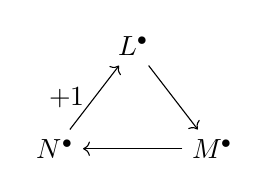
\begin{tikzpicture}[baseline=(current bounding box.center)]
    \node (L) at (1,1.3)
    {$L^\bullet$}; \node (N) at (0,0)
    {$N^\bullet$}; \node (M) at (2,0)
    {$M^\bullet$}; \draw[->] (L) -- (M); \draw[->] (M) -- (N);
    \draw[->] (N) -- (L) node[midway, left] {$+1$};
  \end{tikzpicture}
\]
which we understand to be exact at its three vertices: this is an
\emph{exact triangle} in $\categ{C}(\categ{A})$. The arrow marked by
$+1$ is in this case simply the zero-morphism; the $+1$ records the
fact that we are going to view this as a morphism from $N$ to the
shift $L[1]^\bullet$ of $L^\bullet$ (after all, $0$ is $0$ in all
degrees). Thus, the triangle is shorthand for the impressive
commutative 3D-diagram
% TODO: diagram of the "impressive commutative 3D-diagram" -- a
% stacked lattice showing, for each degree i-1, i, i+1, the triangle
% N^i <-- M^i, with a diagonal 0-arrow N^i -> L^i and vertical arrows
% L^i -> L^{i+1}, M^i -> M^{i+1}, N^i -> N^{i+1} connecting successive
% layers (page 601)
or (understanding the morphisms in the complexes) the single long
sequence
\[
  \dots \longrightarrow N^{i-1} \xrightarrow{0} L^i \longrightarrow
  M^i \longrightarrow N^i \xrightarrow{0} L^{i+1} \longrightarrow
  \dots,
\]
whose exactness is equivalent to the exactness of the original short
exact sequence of complexes. In \S{}3.3 we have obtained from this
\emph{another} long exact sequence,
\[
  \dots \longrightarrow H^{i-1}(N^\bullet) \xrightarrow{\delta^{i-1}}
  H^i(L^\bullet) \longrightarrow H^i(M^\bullet) \longrightarrow
  H^i(N^\bullet) \xrightarrow{\delta^i} H^{i+1}(L^\bullet)
  \longrightarrow \dots,
\]
which we fold again into an exact triangle:
\[
  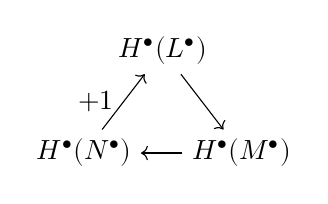
\begin{tikzpicture}[baseline=(current bounding box.center)]
    \node (L) at (1,1.3)
    {$H^\bullet(L^\bullet)$}; \node (N) at (0,0)
    {$H^\bullet(N^\bullet)$}; \node (M) at (2,0)
    {$H^\bullet(M^\bullet)$}; \draw[->] (L) -- (M); \draw[->] (M) --
    (N); \draw[->] (N) -- (L) node[midway, left] {$+1$};
  \end{tikzpicture}
\]
This time the morphism marked $+1$ is the interesting connecting
morphism (while the morphisms in the cohomology complexes are zero;
see the end of \S{}3.2).

Thus, the `long exact cohomology sequence' takes us from a certain
exact triangle to another exact triangle. The first triangle arises
from a short exact sequence of complexes (the `connecting morphism' is
$0$), while the second does not (the connecting morphism is in general
nonzero).

Clearly something interesting is going on. Triangles obtained from
short exact sequences of complexes in $\categ{C}(\categ{A})$ appear to
be `special' and give rise to other exact triangles through
cohomology.

Actually, the situation may make the reader somewhat uncomfortable.
While two sides of the cohomology triangle are obtained by simply
applying the cohomology functor to the corresponding sides of the
original triangle, the third one is obtained by a different process,
involving the connecting morphism. The reader may feel that there
should be a mechanism to go from a triangle defined in terms of an
exact sequence to its counterpart in cohomology by simply applying the
cohomology functor.

This is indeed so. There is an important notion of `distinguished'
triangle, in a category $\categ{K}(\categ{A})$ closely associated with
$\categ{C}(\categ{A})$ and that we will encounter
later\footnote{Beware that some authors call the distinguished
  triangles `exact'; there is some room for confusion, since the
  special exact triangles in the present discussion are not `exact'
  from this viewpoint.} (\S{}5). As with the `special' triangles given
above, distinguished triangles lead to long exact sequences in
cohomology, and in a somewhat more direct fashion. Distinguished
triangles satisfy a number of axioms, which define
$\categ{K}(\categ{A})$ as a \emph{triangulated category}. Exploring
these concepts at any level of depth is well beyond the scope of this
book, but towards the end of the chapter I will try to clarify these
last cryptic remarks (\S{}9.2).

\subsection*{Exercises}

\begin{exer}{\exerused{}}{exer:homol:3.1}
  Let $(M^\bullet, d^\bullet)$ be a resolution of an object $A$ of an
  abelian category. Verify that there are exact complexes
  \[
    \dots \xrightarrow{d^{-3}} M^{-2} \xrightarrow{d^{-2}} M^{-1}
    \longrightarrow \ker d^0 \longrightarrow A \longrightarrow 0
    \longrightarrow \dots,
  \]
  \[
    \dots \longrightarrow 0 \longrightarrow A \longrightarrow
    \cokerd^{-1} \longrightarrow M^1 \xrightarrow{d^1}
    M^2 \xrightarrow{d^2} \dots
  \]
  and that replacing $A$ by $0$ in these complexes produces new
  resolutions of $A$. [\S{}\ref{subsec:homol:reminder-of-basic-definitions-general-strategy}, \S{}\ref{subsec:homol:recovering-a}]
\end{exer}
\begin{exer}{$\lnot$}{exer:homol:3.2}
  Let $\categ{I}$ be the category whose objects are the integers and
  where $\Hom_{\categ{I}}(m, n)$ consists of a singleton if $m \leq n$
  and is $\emptyset$ otherwise (cf.\ \Cref{exam:prelims:set-is-a-category}). Show that the
  category $\categ{C}(\categ{A})$ of cochain complexes is a full
  subcategory of the abelian category $\categ{A}^{\categ{I}}$. [\ref{exer:homol:3.3}]
\end{exer}
\begin{exer}{\exerused{}}{exer:homol:3.3}
  Verify that the category $\categ{C}(\categ{A})$ of cochain complexes
  in an abelian category, defined in \S{}3.2, is itself an abelian
  category. (You can do this either `by hand' or by applying
  Exercises~3.2 and~2.14.) [\S{}\ref{subsec:homol:the-category-of-complexes}]
\end{exer}
\begin{exer}{$\lnot$}{exer:homol:3.4}
  Let $\categ{A}$ be an abelian category. Define a category
  $\operatorname{Seq}(\categ{A})$ whose objects are short exact
  sequences in $\categ{A}$ and where morphisms are commutative
  diagrams
  \[\begin{tikzcd}[column sep=small]
      0 \arrow[r] & A_1 \arrow[r] \arrow[d] & B_1 \arrow[r] \arrow[d]
      &
      C_1 \arrow[r] \arrow[d] & 0 \\
      0 \arrow[r] & A_2 \arrow[r] & B_2 \arrow[r] & C_2 \arrow[r] & 0
    \end{tikzcd}\] Thus, $\operatorname{Seq}(\categ{A})$ may be viewed
  as a full subcategory of $\categ{C}(\categ{A})$.
  \begin{itemize}
  \item Prove that $\operatorname{Seq}(\categ{A})$ is an additive
    category.
  \item Prove that $\operatorname{Seq}(\categ{A})$ has kernels and
    cokernels. (Watch out: these are not the same as in
    $\categ{C}(\categ{A})$. Keep the snake lemma in mind.)
  \item Show that, for every object $X$ of $\categ{A}$,
    \[\begin{tikzcd}[column sep=small]
        0 \arrow[r] & 0 \arrow[r] & X \arrow[r, "\id_X"]
        \arrow[d, "\id_X"'] &
        X \arrow[r] & 0 \\
        0 \arrow[r] & X \arrow[r, "\id_X"'] & X
        \arrow[r] & 0 \arrow[r] & 0 \arrow[from=1-4, to=2-2,
        "\id_X"']
      \end{tikzcd}\] is both a monomorphism and an epimorphism in
    $\operatorname{Seq}(\categ{A})$, although it is neither a
    monomorphism nor an epimorphism in $\categ{C}(\categ{A})$ if
    $X \neq 0$.
  \item Prove that $\operatorname{Seq}(\categ{A})$ is not abelian if
    $\categ{A}$ has nonzero objects.
  \end{itemize} [\S{}\ref{subsec:homol:abelian-categories}, \ref{exer:homol:3.11}]
\end{exer}
\begin{exer}{\exerused{}}{exer:homol:3.5}
  Let $(L^\bullet, d^\bullet_{L^\bullet})$ be a cochain complex;
  define new differentials $d'^\bullet_{L^\bullet}$ by arbitrarily
  changing the sign of $d^i_{L^\bullet}$:
  $d'^i_{L^\bullet} = \pm d^i_{L^\bullet}$. Show that
  $(L^\bullet, d'^\bullet_{L^\bullet})$ is a cochain complex
  isomorphic to $(L^\bullet, d^\bullet_{L^\bullet})$. [\S{}\ref{subsec:homol:the-category-of-complexes}]
\end{exer}
\begin{exer}{}{exer:homol:3.6}
  Provide an arrow-theoretic proof of \Cref{homol:3.4} (cf.\ \Cref{homol:3.1}).
\end{exer}
\begin{exer}{}{exer:homol:3.7}
  Let $\categ{A}$, $\categ{B}$ be abelian categories. An additive
  functor $\mathscr{F} : \categ{A} \to \categ{B}$ is \emph{exact} if
  it maps short exact sequences in $\categ{A}$ to short exact
  sequences in $\categ{B}$. Prove that exact functors commute with
  cohomology: if $\mathscr{F}$ is exact and $L^\bullet$ is a cochain
  complex in $\categ{A}$, then
  $H^\bullet(\mathscr{F}(L^\bullet)) \cong
  \mathscr{F}(H^\bullet(L^\bullet))$, where $\mathscr{F}(L^\bullet)$
  denotes the cochain complex in $\categ{B}$ obtained by applying
  $\mathscr{F}$ to all objects and morphisms in $L^\bullet$.

  In particular, the image of an exact complex through an exact
  functor is still an exact complex (cf.\ \Cref{linrep:exer:1.23}).
\end{exer}
\begin{exer}{\exerused{}}{exer:homol:3.8}
  For any $i$, give an example of a short exact sequence of complexes
  \[
    0 \longrightarrow L^\bullet \longrightarrow M^\bullet
    \longrightarrow N^\bullet \longrightarrow 0
  \]
  such that the sequence
  \[
    0 \longrightarrow H^i(L^\bullet) \longrightarrow H^i(M^\bullet)
    \longrightarrow H^i(N^\bullet) \longrightarrow 0
  \]
  is not exact at either $H^i(L^\bullet)$ or $H^i(N^\bullet)$.
  [\S{}\ref{subsec:homol:universal-property-of-the-derived-functor}]
\end{exer}
\begin{exer}{\exerused{}}{exer:homol:3.9}
  Provide the gory details for the long exact cohomology sequence
  (\Cref{homol:3.5}). [\S{}\ref{subsec:homol:the-long-exact-cohomology-sequence}, \ref{exer:homol:3.10}]
\end{exer}
\begin{exer}{\exerused{}}{exer:homol:3.10}
  Here is a way to reduce \Cref{exer:homol:3.9} to the snake lemma itself.

  Every complex $(L^\bullet, \lambda^\bullet)$ determines a complex
  $\ker^\bullet$, with the object\footnote{Of course $\ker$ and
    $\coker$ mean the target and source of the arrows
    $\ker$ and $\coker$, respectively.}
  $\ker\lambda^{i+1}$ in degree $i$, connected by zero-morphisms, and
  a complex $\coker^\bullet$, with the object
  $\coker\lambda^{i-1}$ in degree $i$, also connected by
  zero-morphisms.

  Prove that $\lambda^\bullet$ induces a morphism
  $\overline{\lambda}^\bullet : \coker^\bullet \to
  \ker^\bullet$ in the abelian category of complexes, such that
  $\ker\overline{\lambda}^\bullet \cong H^\bullet(L^\bullet)$ and
  $\coker\overline{\lambda}^\bullet \cong
  H(L^\bullet)[1]^\bullet$.

  Now work out the whole long exact cohomology sequence as a
  consequence of the snake lemma. (You will use the version of the
  snake lemma given in \Cref{rem:rings:snake-lemma-relaxed-hypotheses}.) [\S{}\ref{subsec:homol:the-long-exact-cohomology-sequence}, \ref{exer:homol:3.13}]
\end{exer}
\begin{exer}{$\lnot$}{exer:homol:3.11}
  Prove that the long exact cohomology sequence is functorial, in the
  sense that it defines a covariant functor from the category
  $\operatorname{Seq}(\categ{C}(\categ{A}))$ of short exact sequences
  (cf.\ \Cref{exer:homol:3.4}) of complexes to the category of
  complexes. [\ref{exer:homol:7.13}]
\end{exer}
\begin{exer}{}{exer:homol:3.12}
  Redo \Cref{exer:rings:7.17}.
\end{exer}
\begin{exer}{}{exer:homol:3.13}
  The viewpoint in \Cref{exer:homol:3.10} admits the following straightforward
  generalization.

  Let $\categ{A}$ be an abelian category. Define a new category
  $d\categ{A}$, whose objects are pairs $(A, d)$, where $A$ is an
  object of $\categ{A}$ and $d : A \to A$ is a morphism (the
  `differential') such that $d^2 = 0$. Morphisms
  $(A, d_A) \to (B, d_B)$ in $d\categ{A}$ are morphisms
  $\varphi : A \to B$ commuting with the differentials:
  $d_B\varphi = \varphi d_A$.
  \begin{itemize}
  \item Prove that $d\categ{A}$ is an abelian category.
  \item For any $(A, d)$ in $d\categ{A}$, prove that $d$ induces a
    morphism $\bar d : \cokerd \to \ker d$.
  \item Define $H(A, d)$ to be $\ker \bar d$. Prove that
    $\coker\bar d \cong H(A, d)$.
  \item Show that $H$ defines an additive functor
    $d\categ{A} \to \categ{A}$ and that this functor is not exact in
    general.
  \item However, prove that every short exact sequence
    \[
      0 \longrightarrow (A, d_A) \longrightarrow (B, d_B)
      \longrightarrow (C, d_C) \longrightarrow 0
    \]
    in $d\categ{A}$ induces an exact triangle (in the sense of
    \S{}3.4)
    \[
      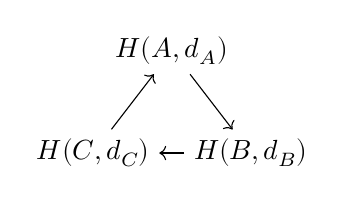
\begin{tikzpicture}[baseline=(current bounding box.center)]
        \node (A) at (1,1.3)
        {$H(A,d_A)$}; \node (C) at (0,0)
        {$H(C,d_C)$}; \node (B) at (2,0)
        {$H(B,d_B)$}; \draw[->] (A) -- (B); \draw[->] (B) -- (C);
        \draw[->] (C) -- (A);
      \end{tikzpicture}
    \]
  \end{itemize}
\end{exer}
\begin{exer}{\exerused{}}{exer:homol:3.14}
  Prove that if one of the vertices of a `special' triangle arising
  from a short exact sequence of complexes (as in \S{}3.4) is exact,
  then the other two vertices have isomorphic cohomologies, possibly
  up to a shift. [\S{}\ref{subsec:homol:the-mapping-cone-of-a-morphism}]
\end{exer}
\begin{exer}{$\lnot$}{exer:homol:3.15}
  Define a `Grothendieck group' and a `universal Euler characteristic'
  $\chi$ for any abelian category $\categ{A}$, in the style of the
  construction given in \ref{subsec:linalg:euler-characteristic-and-the-grothendieck-group}.

  Extend $\chi$ to all bounded cochain complexes $M^\bullet$ in
  $\categ{A}$, by setting
  $\chi(M^\bullet) := \sum_i (-1)^i \chi(M^i)$. Prove that
  $\chi(M^\bullet) = \chi(H^\bullet(M^\bullet))$. For every short
  exact sequence of bounded complexes
  $0 \to L^\bullet \to M^\bullet \to N^\bullet \to 0$, prove that
  $\chi(M^\bullet) = \chi(L^\bullet) + \chi(N^\bullet)$. [\ref{exer:homol:4.3}, \ref{exer:homol:9.1}]
\end{exer}

\section{Cones and homotopies}
\label{sec:homol:cones-and-homotopies}

If $\alpha^\bullet : L^\bullet \to M^\bullet$ is a morphism of cochain
complexes, it is natural to try to describe the morphism induced in
cohomology:
\[
  H^\bullet(\alpha^\bullet) : H^\bullet(L^\bullet) \to
  H^\bullet(M^\bullet).
\]
However, I have pointed out that $H^\bullet$ is not an exact functor,
and this seems to pose an obstacle to simple-minded strategies aimed
at describing (for example) the kernel or cokernel of
$H^\bullet(\alpha^\bullet)$ in terms of the kernel or cokernel of
$\alpha^\bullet$. The long exact cohomology sequence may be used to
compensate for this lack of exactness; we will see how in \S{}4.1. We
will also begin exploring a very important condition (`homotopy')
guaranteeing that two given morphisms of complexes induce the same
morphism in cohomology. Homotopies will be so important that they will
lead us later on to change our notion of morphisms between complexes
and construct a new `homotopic category' of complexes (see \S{}5).

\subsection{The mapping cone of a morphism}
\label{subsec:homol:the-mapping-cone-of-a-morphism}

Let $\alpha^\bullet : L^\bullet \to M^\bullet$ be a morphism of
cochain complexes. The \emph{mapping cone} $MC(\alpha)^\bullet$ of
$\alpha^\bullet$ will allow us to recover $H^\bullet(\alpha^\bullet)$
as the connecting morphism in a long exact cohomology sequence, as
constructed in \S{}3.3. In fact, the mapping cone will give us the
third vertex of a `special' triangle (cf.\ the end of \S{}3.4):
\[
  (\dagger) \quad
  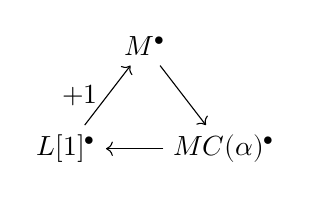
\begin{tikzpicture}[baseline=(current bounding box.center)]
    \node (M) at (1,1.3)
    {$M^\bullet$}; \node (L) at (0,0)
    {$L[1]^\bullet$}; \node (C) at (2,0)
    {$MC(\alpha)^\bullet$}; \draw[->] (M) -- (C); \draw[->] (C) --
    (L); \draw[->] (L) -- (M) node[midway, left] {$+1$};
  \end{tikzpicture}
\]
The degree-increasing morphism is the zero-morphism here (as in the
`special' triangles encountered in \S{}3.4); but taking cohomology
\[
  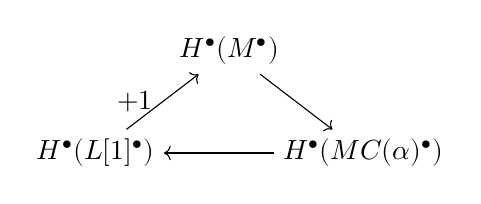
\begin{tikzpicture}[baseline=(current bounding box.center)]
    \node (M) at (1.7,1.3)
    {$H^\bullet(M^\bullet)$}; \node (L) at (0,0)
    {$H^\bullet(L[1]^\bullet)$}; \node (C) at (3.4,0)
    {$H^\bullet(MC(\alpha)^\bullet)$}; \draw[->] (M) -- (C); \draw[->]
    (C) -- (L); \draw[->] (L) -- (M) node[midway, left] {$+1$};
  \end{tikzpicture}
\]
we will obtain morphisms
\[
  H^{i+1}(L^\bullet) = H^i(L[1]^\bullet) \longrightarrow
  H^{i+1}(M^\bullet)
\]
that, I claim, will be nothing but the morphisms induced in cohomology
by the given morphism $\alpha^\bullet$. Thus, the morphisms induced in
cohomology cannot be extended to exact sequences (that would clearly
be asking too much), but they can be extended to triangles arising by
applying cohomology to an appropriate exact sequence of complexes.

Incidentally, the triangle $(\dagger)$ displayed above (but with the
degree-increasing morphism replaced by $-\alpha^\bullet$) will be the
prototype of the `distinguished triangles' mentioned in \S{}3.4 (cf.\
\S{}9.2).

\emph{Construction of the mapping cone.} The objects of
$MC(\alpha)^\bullet$ are simply direct sums of objects of $L^\bullet$
and $M^\bullet$:
\[
  MC(\alpha)^i := L[1]^i \oplus M^i = L^{i+1} \oplus M^i;
\]
but the morphisms
$d^i_{MC(\alpha)^\bullet} : MC(\alpha)^i \to MC(\alpha)^{i+1}$ are not
the `obvious' ones, but rather
\[
  d^i_{MC(\alpha)^\bullet}(\ell, m) := (-d^{i+1}_{L^\bullet}(\ell),
  \alpha^{i+1}(\ell) + d^i_{M^\bullet}(m)).
\]
The sign in the first component is inherited from the shifting of
$L^\bullet$; thus, the first component is simply the differential of
$L[1]^\bullet$. The second component mixes $\alpha^\bullet$ (or rather
its shift $\alpha[1]^\bullet$) and the differential of
$M^\bullet$. The reader should verify that
$d^{i+1}_{MC(\alpha)^\bullet} \circ d^i_{MC(\alpha)^\bullet} = 0$, so
that $MC(\alpha)^\bullet$ is indeed a cochain complex (\Cref{exer:homol:4.1});
this is where the sign comes in. The mapping cone is a special case of
the `total complex' determined by a double complex, to be explored
later (\S{}8.2).

Pictorially, $MC(\alpha)^\bullet$ looks like this:
\[\begin{tikzcd}[column sep=large, row sep=small]
    \dots \arrow[r] & L^{i+1} \arrow[r, "-d^{i+1}_{L^\bullet}"] &
    L^{i+2} \arrow[r] & \dots \\
    & \oplus & \oplus & \\
    \dots \arrow[r] & M^i \arrow[r, "d^i_{M^\bullet}"'] & M^{i+1}
    \arrow[r] & \dots \arrow[from=1-2, to=3-3, "\alpha^{i+1}"
    description]
  \end{tikzcd}\] There are evident morphisms of complexes
$M^\bullet \to MC(\alpha)^\bullet$ and
$MC(\alpha)^\bullet \to L[1]^\bullet$, induced by the natural
morphisms
$M^i \longrightarrow L^{i+1} \oplus M^i \longrightarrow
L^{i+1}$. Since the sequences
\[
  0 \longrightarrow M^i \longrightarrow L[1]^i \oplus M^i
  \longrightarrow L[1]^i \longrightarrow 0
\]
are all exact, the sequence of complexes
\[
  0 \longrightarrow M^\bullet \longrightarrow MC(\alpha)^\bullet
  \longrightarrow L[1]^\bullet \longrightarrow 0
\]
is exact.
\begin{prop}{}{homol:4.1}
  There is an exact triangle
  \[
    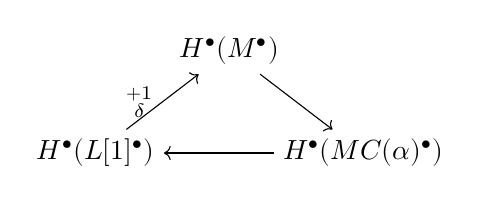
\begin{tikzpicture}[baseline=(current bounding box.center)]
      \node (M) at (1.7,1.3)
      {$H^\bullet(M^\bullet)$}; \node (L) at (0,0)
      {$H^\bullet(L[1]^\bullet)$}; \node (C) at (3.4,0)
      {$H^\bullet(MC(\alpha)^\bullet)$}; \draw[->] (M) -- (C);
      \draw[->] (C) -- (L); \draw[->] (L) -- (M) node[midway, left]
      {$\substack{+1 \\ \delta}$};
    \end{tikzpicture}
  \]
  where the connecting morphism $\delta$ is the morphism induced by
  $\alpha^\bullet$ in cohomology.
\end{prop}

\begin{proof}
  The existence of the triangle is a direct consequence of
  \Cref{homol:3.5}; all we have to check is that the connecting morphism
  indeed agrees with the morphism induced by $\alpha^\bullet$.
  Chasing the diagram
  \[\begin{tikzcd}[column sep=small]
      & \vdots & \vdots & \vdots & \\
      0 \arrow[r] & M^i \arrow[r] \arrow[u] &
      L^{i+1} \oplus M^i \arrow[r] \arrow[u] & L^{i+1} \arrow[r] \arrow[u] & 0 \\
      0 \arrow[r] & M^{i-1} \arrow[r] \arrow[u] &
      L^i \oplus M^{i-1} \arrow[r] \arrow[u] & L^i \arrow[r] \arrow[u] & 0 \\
      & \vdots \arrow[u] & \vdots \arrow[u] & \vdots \arrow[u] &
    \end{tikzcd}\] with a class in
  $H^{i-1}(L[1]^\bullet) = H^i(L^\bullet)$ represented by
  $\ell \in L^i$ (such that $d^i_{L^\bullet}(\ell) = 0$), we find that
  $\alpha^i(\ell)$, viewed as an element of $MC(\alpha)^i$ via
  $(0, \alpha^i(\ell))$, is cohomologous to $(\ell, 0)$,
  % TODO: diagram chase verifying (0, alpha^i(ell)) and (ell, 0)
  % represent the same class in MC(alpha)^i (page 607)
  which maps to $\ell$ under $MC(\alpha)^\bullet \to L[1]^\bullet$;
  this verifies the claim.
\end{proof}

\begin{coro}{}{homol:4.2}
  Let $\alpha^\bullet : L^\bullet \to M^\bullet$ be a morphism of
  cochain complexes. Then the induced morphism
  $H^\bullet(L^\bullet) \to H^\bullet(M^\bullet)$ is an isomorphism if
  and only if the mapping cone $MC(\alpha)^\bullet$ is an exact
  complex.

  (Cf.\ \Cref{exer:homol:3.14}.)
\end{coro}

I should mention that mapping cones arose in topology: the mapping
cone of a continuous map $f : X \to Y$ is obtained by considering
$X \times [0,1]$, identifying $X \times 0$ to a point, and stitching
$X \times 1$ to $Y$ by means of $f$. Analyzing chains of this space
leads to the (homological version of the) `algebraic' mapping cone
considered above.

\subsection{Quasi-isomorphisms and derived categories}
\label{subsec:homol:quasi-isomorphisms-and-derived-categories}

A component of our main strategy consists of understanding when
cochain complexes `have a good reason' to have the same cohomology.
\Cref{homol:4.2} provides us with such a reason. The morphisms singled
out in that statement have a name:

\begin{defn}{}{homol:4.3}
  A morphism $\alpha^\bullet$ of cochain complexes is a
  \emph{quasi-isomorphism} if it induces an isomorphism in cohomology.
\end{defn}

By \Cref{homol:4.2}, this condition is equivalent to the exactness of the
mapping cone of $\alpha^\bullet$.

\begin{exam}{}{homol:4.4}
  The datum of a resolution $M^\bullet$ of an object $A$ of an abelian
  category $\categ{A}$, as in \Cref{homol:3.2} and with $M^i = 0$ for
  $i > 0$, is the same as the datum of a quasi-isomorphism
  \[
    M^\bullet \xrightarrow{\text{q-iso.}} \iota(A)
  \]
  where $\iota$ places $A$ in degree $0$ and $0$ in all other
  degrees. Here is a larger version of the same diagram:
  \[\begin{tikzcd}[column sep=small]
      \dots \arrow[r] & M^{-2} \arrow[r, "d^{-2}_{M^\bullet}"]
      \arrow[d] & M^{-1} \arrow[r, "d^{-1}_{M^\bullet}"] \arrow[d] &
      M^0 \arrow[r, "d^0_{M^\bullet}"] \arrow[d] & 0 \arrow[r] \arrow[d] & \dots \\
      \dots \arrow[r] & 0 \arrow[r] & 0 \arrow[r] & A \arrow[r] & 0
      \arrow[r] & \dots
    \end{tikzcd}\] where the only nontrivial vertical map is the
  cokernel of $d^{-1}_{M^\bullet}$.
\end{exam}

Thus, quasi-isomorphisms may be viewed as generalizations of more
simple-minded resolutions. Also note that the mapping cone of a
resolution as in \Cref{homol:4.4} is obtained (as the reader should check)
by shifting the complex `one step to the left' and completing it with
$A$, obtaining the \emph{exact} complex:
\[
  \dots \longrightarrow M^{-1} \xrightarrow{-d^{-1}_{M^\bullet}} M^0
  \xrightarrow{\cokerd^{-1}_{M^\bullet}} A
  \longrightarrow 0 \longrightarrow \dots.
\]
This is nothing but our other point of view on resolutions (as in
\ref{subsec:linalg:finitely-presented-modules-and-free-resolutions}).

\begin{rem}{}{homol:4.5}
  Quasi-isomorphisms with fixed target (resp., source) form a category
  in a natural way, which I will leave to the reader to make
  precise. In particular, resolutions in
  $\categ{C}^{\leq 0}(\categ{A})$ (resp.,
  $\categ{C}^{\geq 0}(\categ{A})$) of a given object of $\categ{A}$,
  as in \Cref{homol:4.4}, form a category.
\end{rem}

Wouldn't it be nice if quasi-isomorphisms were actual isomorphisms,
that is, if they were invertible? In general, they are not. The
following example will arise several times to ward off any such hopes.

\begin{exam}{}{homol:4.6}
  In $\categ{C}(\categ{Ab})$, the morphism of complexes
  \[\begin{tikzcd}[column sep=small]
      \dots \arrow[r] & 0 \arrow[r] \arrow[d] & \Z \arrow[r, "\cdot
      2"] \arrow[d] &
      \Z \arrow[r] \arrow[d, "\pi"] & 0 \arrow[r] \arrow[d] & \dots \\
      \dots \arrow[r] & 0 \arrow[r] & 0 \arrow[r] & \dfrac{\Z}{2\Z}
      \arrow[r] & 0 \arrow[r] & \dots
    \end{tikzcd}\] where $\pi$ is the natural projection, is a
  quasi-isomorphism, but it does not have an inverse since there are
  no nontrivial homomorphisms $\Z/2\Z \to \Z$.
\end{exam}

In fact, this example shows that `quasi-isomorphism' is not even an
equivalence relation (it is not symmetric). This is too bad---if it
were, then the `equivalence class of a complex' would be the most
natural candidate for the entity carrying the maximal amount of
cohomological information of a complex.

I will stop short of defining a `quasi-isomorphism relation': in this
book, quasi-isomorphism is simply a particular quality of a morphism
of cochain complexes, not a relation. In any case recall that, even in
the context of sets, taking the quotient by an equivalence relation is
not the `primary' object of interest: the quotient is just the
solution to the natural universal problem of studying functions to
other sets with identical behavior on `equivalent'
elements. \emph{This} is the primary objective.

Similarly, the primary objective in the present context is not so much
to identify together all complexes linked by a quasi-isomorphism, as
it is to be able to shuttle information back and forth between such
complexes. The natural way to accomplish this is to study environments
in which quasi-isomorphisms do have inverses. More precisely, it
consists of studying additive functors
\[
  \mathscr{F} : \categ{C}(\categ{A}) \longrightarrow \categ{D}
\]
such that $\mathscr{F}(\rho^\bullet)$ is an isomorphism for every
quasi-isomorphism $\rho^\bullet$. (Cohomology is such a functor.)

This sounds like yet another universal problem, and the natural line
of attack would be to solve it as such, that is, to define (if
possible) a category $\categ{D}(\categ{A})$ endowed with an additive
functor $\categ{C}(\categ{A}) \to \categ{D}(\categ{A})$ such that
quasi-isomorphisms in $\categ{C}(\categ{A})$ are mapped to
isomorphisms in $\categ{D}(\categ{A})$ and through which every
$\mathscr{F}$ as above must factor uniquely:
\[\begin{tikzcd}
    \categ{C}(\categ{A}) \arrow[r, "\mathscr{F}"] \arrow[d] & \categ{D} \\
    \categ{D}(\categ{A}) \arrow[ur, dashed, "\exists!"']
  \end{tikzcd}\] To be honest, we should take such a statement with a
grain of salt: the natural environment in which we should pose this
universal problem would be a `category of categories', and we have not
defined such a thing in this book. A category $\categ{D}(\categ{A})$
as above \emph{does} exist, at least if a certain `localization'
process can be carried out\footnote{There may be set-theoretic issues
  with this process. However, these play no role in the cases we will
  consider, in which $\categ{A}$ has `enough projectives' or `enough
  injectives'.}: it is the \emph{derived category} of $\categ{A}$.
`Bounded' versions $\categ{D}^-(\categ{A})$, $\categ{D}^+(\categ{A})$,
and more, are solutions to the corresponding universal problems for
appropriately bounded complexes.

These derived categories answer the main question underlying our
strategy, of understanding `what' in a complex really determines its
cohomology: the answer amounts to viewing the complex in the
appropriate derived category. The construction of
$\categ{D}(\categ{A})$ consists roughly of taking the same objects as
$\categ{C}(\categ{A})$ and formally inverting the
quasi-isomorphisms. The details of this construction are somewhat
involved and are best left to more advanced texts. But we will be able
to capture its essence in this book, at least in lucky cases (when the
abelian category has `enough injectives' or `enough projectives'; see
\Cref{defn:homol:5.7}).

The derived category has the unfortunate reputation of being an overly
abstract notion, and there are fundamental questions about whether it
really is the best approach to an abstract study of cohomology. This
is partly because the derived category of an abelian category is
\emph{not} an abelian category and simple notions such as kernel,
cokernel, exact sequences are not available in
$\categ{D}(\categ{A})$. This adds a substantial layer of complication
to the theory.

On the other hand, going past these difficulties, one finds that
enough structure remains to do much homological algebra: objects in
$\categ{D}(\categ{A})$ have cohomology, and there are `distinguished
triangles' (cf.\ \S{}3.4) abstracting exact sequences and giving long
exact cohomology sequences. The derived category is a
\emph{triangulated category}, like the more manageable homotopic
category $\categ{K}(\categ{A})$ that we will soon define. Its uses go
beyond the confines of algebra or even mathematics: an approach to the
understanding of `D-branes' in string theory is based on derived
categories.

To get a sense of how counterintuitive $\categ{D}(\categ{A})$ must be,
note that the zero-morphism $0 : M^\bullet \to M^\bullet$ may well be
a quasi-isomorphism: in fact, this is so precisely when $M^\bullet$ is
exact. Well, in any category $\categ{D}$ as above (and in particular
in the derived category $\categ{D}(\categ{A})$) this zero-morphism
remains the zero-morphism, \emph{but} it comes equipped with an
inverse when it is a quasi-isomorphism. Thus, in the derived category
the zero-morphism on a complex involving nonzero objects may well be
invertible! This says that complexes that are nonzero in
$\categ{C}(\categ{A})$ may become zero-objects in the derived
category.

\begin{lem}{}{homol:4.7}
  Let $\categ{D}$ be an additive category, and let
  $\mathscr{F} : \categ{C}(\categ{A}) \to \categ{D}$ be an additive
  functor such that $\mathscr{F}(\rho^\bullet)$ is an isomorphism for
  every quasi-isomorphism $\rho^\bullet$.
  \begin{itemize}
  \item Let $M^\bullet$ be an exact complex in $\categ{C}(\categ{A})$.
    Then the complex $\mathscr{F}(M^\bullet)$, obtained by applying
    $\mathscr{F}$ to the objects and morphisms of $M^\bullet$, is a
    zero-object in $\categ{D}$.
  \item Let $\alpha^\bullet : L^\bullet \to N^\bullet$ be a morphism
    in $\categ{C}(\categ{A})$ that factors through an exact complex,
    \[\begin{tikzcd}
        L^\bullet \arrow[rr, "\alpha^\bullet"] \arrow[dr] & & N^\bullet \\
        & M^\bullet \arrow[ur]
      \end{tikzcd}\] with $M^\bullet$ exact. Then
    $\mathscr{F}(\alpha^\bullet)$ is the zero-morphism.
  \end{itemize}
\end{lem}

\begin{proof}
  The second claim follows from the first, since by applying
  $\mathscr{F}$ to the given diagram we obtain
  \[\begin{tikzcd}
      \mathscr{F}(L^\bullet) \arrow[rr, "\mathscr{F}(\alpha^\bullet)"]
      \arrow[dr] & & \mathscr{F}(N^\bullet) \\
      & \mathscr{F}(M^\bullet) \arrow[ur]
    \end{tikzcd}\] and we see that $\mathscr{F}(\alpha^\bullet)$
  factors through a zero-object of $\categ{D}$.

  To verify the first claim, note that since $M^\bullet$ is exact, the
  zero-morphism $M^\bullet \to M^\bullet$ is a quasi-isomorphism;
  hence it is mapped to an invertible morphism by $\mathscr{F}$:
  \[
    \underbrace{\mathscr{F}(M^\bullet) \xrightarrow{\mathscr{F}(0)}
      \mathscr{F}(M^\bullet) \xrightarrow{\mathscr{F}(0)^{-1}}
      \mathscr{F}(M^\bullet)}_{\id_{\mathscr{F}(M^\bullet)}}
  \]
  Since $\mathscr{F}$ is additive, $\mathscr{F}(0) = 0$. It follows
  that $\id_{\mathscr{F}(M^\bullet)} = 0$ and hence that
  $\mathscr{F}(M^\bullet)$ is a zero-object of $\categ{D}$, by
  \Cref{exer:homol:1.6}.
\end{proof}

In the next several sections I will chase the notion of derived
category, aiming to understand it rather concretely in particularly
favorable circumstances. \emph{We will take it for granted that these
  categories exist.} A detailed definition of these objects, or a
treatment of triangulated categories, is beyond the scope of this
book.

\subsection{Homotopy}
\label{subsec:homol:homotopy}

The foregoing considerations put our strategy into focus: we are after
constructions that determine cochain complexes `up to
quasi-isomorphism'. However, quasi-isomorphisms appear hard to deal
with directly. Thus, we look for more manageable notions that may work
as an effective replacement.

Like the mapping cone, this line of approach also owes its origins to
topology: in topology, `homeomorphism' is often too harsh a
requirement, while `homotopy equivalence' is a more malleable but
still adequate notion. For example, homotopy equivalent topological
spaces have the same homology. Distilling the algebra out of this
notion leads to an analog at the level of complexes.

To see how this is done, recall that if $f$, $g$ are \emph{homotopic}
continuous functions between two topological spaces $X$ and $Y$, then
$f$ and $g$ induce the same map on the homology of the spaces.  To
remind yourself of how this works, look at the picture:
% TODO: diagram of a homotopy h(a) between f(a) and g(a): a
% curved/wavy region bounded by f(a) on the left, g(a) on the right,
% delta_+ on top and delta_- on bottom, with h(a) labeling the
% interior surface (page 611)
This is supposed to represent the action of a homotopy between $f$ and
$g$ on a chain $a$ in $X$: $h(a)$ is obtained by mapping
$a \times [0,1]$ to $Y$ so as to get $f(a)$ when restricting to
$a \times \{0\}$ and to get $g(a)$ when restricting to
$a \times \{1\}$. Note that $h(a)$ is a chain of dimension $1$ higher
than the dimension of $a$, and that the boundary $\partial h(a)$ of
this chain consists of $f(a)$, $g(a)$ and of the restriction of $h$ to
the boundary $\partial a$ of $a$: taking the boundary
`counterclockwise',
\[
  \partial h(a) = g(a) - \delta_+ - f(a) + \delta_- = g(a) - f(a) -
  h(\partial a)
\]
(or so it would seem from the picture! As presented here, this is of
course at best a plausibility argument; it can be made rigorous, but
that is someone else's business). That is,
\[
  g(a) - f(a) = \partial h(a) + h(\partial a).
\]
Since boundaries vanish in homology, $f(a)$ and $g(a)$ will agree in
homology.

Here is the translation into algebra of this pleasant geometric
situation:

\begin{defn}{}{homol:4.8}
  A \emph{homotopy} $h$ between two morphisms of cochain complexes
  $\alpha^\bullet, \beta^\bullet : L^\bullet \to M^\bullet$ is a
  collection of morphisms
  \[
    h^i : L^i \to M^{i-1}
  \]
  such that $\forall i$
  \[
    \beta^i - \alpha^i = d^{i-1}_{M^\bullet} \circ h^i + h^{i+1} \circ
    d^i_{L^\bullet}.
  \]
  We say that $\alpha^\bullet$ is \emph{homotopic} to $\beta^\bullet$
  and write $\alpha^\bullet \sim \beta^\bullet$ if there is a homotopy
  between $\alpha^\bullet$ and $\beta^\bullet$.
\end{defn}

We are dealing here with cochain complexes; this accounts for the fact
that while in the topological situation (where we were interested in
\emph{chains} rather than cochains) the homotopy would shift
dimensions up, in \Cref{homol:4.8} it shifts degrees down.

Aside from its topological motivation, homotopy is not too easy to
visualize. The following diagram is \emph{not} assumed to be
commutative:
% TODO: diagram of the non-commutative "lozenge" picture for a
% homotopy h between alpha^bullet, beta^bullet: L^bullet -> M^bullet
% -- two parallel rows of the complexes L^i and M^i connected by d_L,
% d_M horizontally, alpha^i/beta^i vertically, and h^i diagonally (L^i
% -> M^{i-1}), with lozenge shapes drawn between each pair of
% alpha^i/beta^i arrows to emphasize non-commutativity (page 612)
The morphisms $h^i$ do not usually define a morphism of complexes
$L^\bullet \to M[-1]^\bullet$: the lozenges in this diagram are not
required to commute.

\begin{defn}{}{homol:4.9}
  A morphism $\alpha^\bullet : L^\bullet \to M^\bullet$ is a
  \emph{homotopy equivalence} if there is a morphism
  $\beta^\bullet : M^\bullet \to L^\bullet$ such that
  $\alpha^\bullet \circ \beta^\bullet \sim 1_{M^\bullet}$ and
  $\beta^\bullet \circ \alpha^\bullet \sim 1_{L^\bullet}$. The
  complexes $L^\bullet$, $M^\bullet$ are said to be \emph{homotopy
    equivalent} if there is a homotopy equivalence
  $L^\bullet \to M^\bullet$.
\end{defn}

The reader should check that $\sim$ is an equivalence relation and
that `homotopy equivalence of complexes' is also (\Cref{exer:homol:4.4}).
Further, these relations are clearly compatible with simple operations
of morphisms (Exercises~4.5 and~4.6).

\begin{prop}{}{homol:4.10}
  If $\alpha^\bullet, \beta^\bullet : L^\bullet \to M^\bullet$ are
  homotopic morphisms of complexes, then $\alpha^\bullet$,
  $\beta^\bullet$ induce the same morphisms on cohomology:
  $H^\bullet(L^\bullet) \to H^\bullet(M^\bullet)$.
\end{prop}

\begin{proof}
  Let $\bar\ell \in H^i(L^\bullet)$. Then $\bar\ell$ is represented by
  an element $\ell \in \ker(d^i_{L^\bullet})$, and its images in
  $H^i(M^\bullet)$ under the morphisms induced by $\alpha^\bullet$,
  $\beta^\bullet$ are represented by $\alpha^i(\ell)$,
  $\beta^i(\ell)$. Since $\alpha^\bullet$, $\beta^\bullet$ are
  homotopic, according to \Cref{homol:4.8} there are morphisms $h^i$
  such that
  \[
    \beta^i(\ell) - \alpha^i(\ell) = d^{i-1}_{M^\bullet}(h^i(\ell)) +
    h^{i+1}(d^i_{L^\bullet}(\ell)).
  \]
  Since $\ell \in \ker d^i_{L^\bullet}$, the last term vanishes. This
  shows that
  \[
    \beta^i(\ell) - \alpha^i(\ell) \in
    \imaged^i_{M^\bullet},
  \]
  proving that $\beta^i(\ell) - \alpha^i(\ell)$ vanishes in
  $H^i(M^\bullet)$, as needed.
\end{proof}

For example, if $\alpha^\bullet$ is homotopic to the identity, then by
\Cref{homol:4.2} the cone of $\alpha^\bullet$ must be exact. It is a good
exercise to verify this fact directly (\Cref{exer:homol:4.8}).

\begin{coro}{}{homol:4.11}
  Homotopy equivalent complexes have isomorphic cohomology.
\end{coro}

\begin{proof}
  Indeed, morphisms $\alpha^\bullet : L^\bullet \to M^\bullet$,
  $\beta^\bullet : M^\bullet \to L^\bullet$ such that
  $\beta^\bullet \circ \alpha^\bullet$ and
  $\alpha^\bullet \circ \beta^\bullet$ are both homotopic to the
  identity induce inverse morphisms in cohomology, by
  \Cref{homol:4.10}.
\end{proof}

\begin{rem}{}{homol:4.12}
  In other words, homotopy equivalences of complexes are
  quasi-isomorphisms. This does not yet solve the `problem' that
  quasi-isomorphisms are not invertible, since \Cref{homol:4.6} shows that
  quasi-isomorphisms may well not be invertible even up to homotopy.
  In other words, `homotopy equivalence' is a more restrictive notion
  than `quasi-isomorphism'. One reason to study complexes of
  injective/projective modules, as we will do in \S{}5.3, is precisely
  that quasi-isomorphism and homotopy equivalence are equivalent
  notions for (bounded) complexes of injective or projective
  modules. Since homotopy equivalence is a ready-made equivalence
  relation on complexes, this will bypass any technicality needed to
  make sense of `quasi-isomorphism' as an equivalence relation.
\end{rem}

\Cref{homol:4.11} is the main technical reason that makes the strategy
presented in \S{}3.1 work, in a class of interesting examples. As we
will see in due time, in these examples the cohomology of the relevant
cochain complexes will end up being independent of the choices,
because these choices will produce homotopic complexes.

Another key observation will be that homotopy equivalence is preserved
by any additive functor. Suppose $\categ{A}$, $\categ{B}$ are abelian
categories and
\[
  \mathscr{F} : \categ{A} \longrightarrow \categ{B}
\]
is an additive functor (\Cref{homol:1.1}). Then $\mathscr{F}$ induces an
additive functor preserving the grading
\[
  \categ{C}(\mathscr{F}) : \categ{C}(\categ{A}) \longrightarrow
  \categ{C}(\categ{B}).
\]

\begin{lem}{}{homol:4.13}
  With $\mathscr{F}$ as above, if $\alpha^\bullet \sim \beta^\bullet$
  in $\categ{C}(\categ{A})$, then
  $\categ{C}(\mathscr{F})(\alpha^\bullet) \sim
  \categ{C}(\mathscr{F})(\beta^\bullet)$ in $\categ{C}(\categ{B})$,
  and if $L^\bullet$ and $M^\bullet$ are homotopy equivalent complexes
  in $\categ{C}(\categ{A})$, then $\categ{C}(\mathscr{F})(L^\bullet)$
  and $\categ{C}(\mathscr{F})(M^\bullet)$ are homotopy equivalent
  complexes in $\categ{C}(\categ{B})$.
\end{lem}

\begin{proof}
  The second assertion follows from the first. The first is an
  immediate consequence of the fact that $\mathscr{F}$ is additive.
  Indeed, if $h$ is a homotopy between
  $\alpha^\bullet, \beta^\bullet : L^\bullet \to M^\bullet$, then
  \[
    \beta^i - \alpha^i = d^{i-1}_{M^\bullet} \circ h^i + h^{i+1} \circ
    d^i_{L^\bullet}.
  \]
  Since $\mathscr{F}$ preserves the additive structure on Hom-sets,
  this implies
  \[
    \mathscr{F}(\beta^i) - \mathscr{F}(\alpha^i) =
    \mathscr{F}(d^{i-1}_{M^\bullet}) \circ \mathscr{F}(h^i) +
    \mathscr{F}(h^{i+1}) \circ \mathscr{F}(d^i_{L^\bullet}),
  \]
  showing that the collection of morphisms $\mathscr{F}(h^i)$ gives a
  homotopy between $\mathscr{F}(\alpha^\bullet)$ and
  $\mathscr{F}(\beta^\bullet)$.
\end{proof}

Note that the analogous statement does \emph{not} hold for
quasi-isomorphisms (\Cref{exer:homol:4.15}): an additive functor does not
preserve quasi-isomorphisms (while an exact functor does).

\Cref{homol:4.13} implies that the conclusion of \Cref{homol:4.11} holds true
after applying an additive functor:

\begin{thm}{}{homol:4.14}
  Let $\mathscr{F} : \categ{A} \to \categ{B}$ be an additive functor
  between two abelian categories. If $L^\bullet$, $M^\bullet$ are
  homotopy equivalent complexes in $\categ{C}(\categ{A})$, then the
  cohomology complexes
  \[
    H^\bullet(\categ{C}(\mathscr{F})(L^\bullet)), \quad
    H^\bullet(\categ{C}(\mathscr{F})(M^\bullet))
  \]
  are isomorphic.
\end{thm}

The proof of this statement is essentially immediate after all our
preparatory work, so it is left to the reader (\Cref{exer:homol:4.16}).

I am gracing this statement with theorem status because it is at the
root of the strategy I am pursuing. The content of \Cref{homol:4.14} is
that any mechanism associating to a mathematical object a cochain
complex determined up to homotopy will give rise to a slew of
interesting invariants: apply your favorite additive functor to any
such complex, take cohomology, and \Cref{homol:4.14} guarantees that the
result will be independent of the specific chosen complex. This is
(part of) the reason underlying the various claims of independence on
choices made in \ref{subsec:linrep:the-tor-functors} and \ref{subsec:linrep:the-ext-functors}, concerning the
definition of the Tor and Ext functors, as we will see later in the
chapter (\S{}7, especially Examples~7.6 and~7.7).

\subsection*{Exercises}

\begin{exer}{\exerused{}}{exer:homol:4.1}
  Verify that the cone of a morphism of complexes is a complex.
  [\S{}\ref{subsec:homol:the-mapping-cone-of-a-morphism}]
\end{exer}
\begin{exer}{}{exer:homol:4.2}
  Let $L^\bullet = \dots \to 0 \to L \to 0 \to \dots$ and
  $M^\bullet = \dots \to 0 \to M \to 0 \to \dots$ be two complexes
  concentrated in degree $0$. Giving a morphism
  $\alpha^\bullet : L^\bullet \to M^\bullet$ is then the same as
  giving a morphism $\alpha : L \to M$. Describe the mapping cone in
  this case and its cohomology.
\end{exer}
\begin{exer}{}{exer:homol:4.3}
  Let $\alpha^\bullet : L^\bullet \to M^\bullet$ be a morphism of
  bounded complexes. Note that the mapping cone $MC(\alpha)^\bullet$
  of $\alpha$ is also bounded; thus, the three complexes $L^\bullet$,
  $M^\bullet$, $MC(\alpha)^\bullet$ have a well-defined universal
  Euler characteristic (see \Cref{exer:homol:3.15}). Prove that
  \[
    \chi(MC(\alpha)^\bullet) = \chi(M^\bullet) - \chi(L^\bullet).
  \]
\end{exer}
\begin{exer}{\exerused{}}{exer:homol:4.4}
  Prove that the homotopy relation between morphisms of complexes and
  the relation of homotopy equivalence between complexes are
  equivalence relations. [\S{}\ref{subsec:homol:homotopy}, \S{}\ref{sec:homol:projective-and-injective-resolutions-and-the-derived-category}]
\end{exer}
\begin{exer}{\exerused{}}{exer:homol:4.5}
  Let
  $\alpha_k^\bullet, \beta_k^\bullet : L^\bullet_k \to M_k^\bullet$,
  $k = 0, 1$, be morphisms of cochain complexes. Assume that
  $\alpha_0 \sim \beta_0$, $\alpha_1 \sim \beta_1$. Prove that
  $\alpha_0 \oplus \alpha_1 \sim \beta_0 \oplus \beta_1$ as morphisms
  $L^\bullet_0 \oplus L^\bullet_1 \to M_0^\bullet \oplus M_1^\bullet$.
  [\S{}\ref{subsec:homol:homotopy}]
\end{exer}
\begin{exer}{\exerused{}}{exer:homol:4.6}
  Let
  $\alpha^\bullet, \alpha_0^\bullet, \alpha_1^\bullet : L^\bullet \to
  M^\bullet$ and
  $\beta^\bullet, \beta_0^\bullet, \beta_1^\bullet : M^\bullet \to
  N^\bullet$ be morphisms of cochain complexes.
  \begin{enumerate}[label=(\roman*)]
  \item Assume that $\alpha^\bullet \sim 0$ or $\beta^\bullet \sim 0$.
    Prove that $\beta^\bullet \circ \alpha^\bullet \sim 0$.
  \item Assume that $\alpha_0^\bullet \sim \alpha_1^\bullet$ and
    $\beta_0^\bullet \sim \beta_1^\bullet$. Prove that
    $\beta_0^\bullet \circ \alpha_0^\bullet \sim \beta_1^\bullet \circ
    \alpha_1^\bullet$.

    (Hint: Use (i), while thinking about ideals.)
  \end{enumerate} [\S{}\ref{subsec:homol:homotopy}, \S{}\ref{subsec:homol:definition-of-the-homotopic-category-of-complexes}, \S{}\ref{subsec:homol:homotopy-equivalences-vs-quasi-isomorphisms-in-k-a}, \S{}\ref{subsec:homol:proof-of-theorem-5-9}]
\end{exer}
\begin{exer}{}{exer:homol:4.7}
  Prove that the equivalence class of morphisms of complexes
  $L^\bullet \to M^\bullet$ homotopic to a given morphism is
  parametrized by the set of collections of morphisms
  $h^i : L^i \to M^{i-1}$, modulo the morphisms of complexes
  $L[1]^\bullet \to M^\bullet$.
\end{exer}
\begin{exer}{\exerused{}}{exer:homol:4.8}
  Let $\alpha^\bullet$ be a morphism of complexes, homotopic to the
  identity. Prove directly (without appealing to \Cref{homol:4.2}) that
  the mapping cone of $\alpha^\bullet$ is exact. [\S{}\ref{subsec:homol:homotopy}]
\end{exer}
\begin{exer}{$\lnot$}{exer:homol:4.9}
  Let $\alpha^\bullet : L^\bullet \to M^\bullet$ be a morphism of
  cochain complexes. The \emph{mapping cylinder}
  $MCyl(\alpha)^\bullet$ is the cochain complex with objects
  $L^i \oplus L^{i+1} \oplus M^i$ in degree $i$ and differential
  $d^\bullet_{MCyl(\alpha)^\bullet}$ defined by
  \[
    d^i_{MCyl(\alpha)^\bullet}(\ell, \ell', m) =
    (d^i_{L^\bullet}(\ell) + \ell', -d^{i+1}_{L^\bullet}(\ell'),
    \alpha^{i+1}(\ell') + d^i_{M^\bullet}(m)).
  \]
  Verify that
  $d^{i+1}_{MCyl(\alpha)^\bullet} \circ d^i_{MCyl(\alpha)^\bullet} =
  0$ and hence that $MCyl(\alpha)^\bullet$ is indeed a cochain
  complex. [\ref{exer:homol:4.10}, \ref{exer:homol:4.11}, \ref{exer:homol:4.12}, \ref{exer:homol:4.13}]
\end{exer}
\begin{exer}{}{exer:homol:4.10}
  Topologically speaking, the mapping cylinder of a continuous map
  $f : X \to Y$ is obtained by considering $X \times [0,1]$ and gluing
  $X \times 1$ to $Y$ by means of $f$; studying (co)chains of this
  object leads to the algebraic mapping cylinder of \Cref{exer:homol:4.9}.

  As we learn in topology, two continuous maps $X \to Y$ are homotopic
  if they may be realized as the restrictions to $X \times 0$,
  $X \times 1$ of a continuous map from the cylinder $X \times [0,1]$
  to $Y$. Note that this cylinder is the mapping cylinder of
  $\id_X$.

  Prove that two cochain maps
  $\alpha^\bullet, \beta^\bullet : L^\bullet \to M^\bullet$ are
  homotopic in the sense of \Cref{homol:4.8} if and only if they extend
  to a cochain morphism
  $(-\alpha^\bullet, h^\bullet, \beta^\bullet) :
  MCyl(\id_{L^\bullet}) \to M^\bullet$.
\end{exer}
\begin{exer}{$\lnot$}{exer:homol:4.11}
  In topology, the mapping cone may be obtained by contracting
  $X \times 0$ to a point in the mapping cylinder (cf.\ \Cref{exer:homol:4.9}
  and the description of the mapping cone given in \S{}4.1).

  In the algebraic version, this contraction amounts to mod-ing out
  the first component of $MCyl(\alpha)^\bullet$. For a cochain
  morphism $\alpha^\bullet : L^\bullet \to M^\bullet$, prove that
  there is an exact sequence of cochain complexes
  \[
    0 \longrightarrow L^\bullet \longrightarrow MCyl(\alpha)^\bullet
    \longrightarrow MC(\alpha)^\bullet \longrightarrow 0.
  \] [\ref{exer:homol:4.14}]
\end{exer}
\begin{exer}{$\lnot$}{exer:homol:4.12}
  With notation as in \Cref{exer:homol:4.9} (in particular, for a cochain
  morphism $\alpha^\bullet : L^\bullet \to M^\bullet$), prove that
  there is an exact sequence of cochain complexes
  \[
    0 \longrightarrow M^\bullet \longrightarrow MCyl(\alpha)^\bullet
    \longrightarrow MC(\id_{L^\bullet})^\bullet
    \longrightarrow 0.
  \]
  Deduce that there is a quasi-isomorphism
  $M^\bullet \to MCyl(\alpha)^\bullet$. [\ref{exer:homol:4.13}, \ref{exer:homol:4.14}]
\end{exer}
\begin{exer}{$\lnot$}{exer:homol:4.13}
  Still with notation as in \Cref{exer:homol:4.9}, define maps
  $\rho^\bullet : M^\bullet \to MCyl(\alpha)^\bullet$ and
  $\sigma^\bullet : MCyl(\alpha)^\bullet \to M^\bullet$ by
  \[
    \rho^i(m) = (0, 0, m), \qquad \sigma^i(\ell, \ell', m) = m -
    \alpha^i(\ell).
  \]
  Prove that $\rho^\bullet$, $\sigma^\bullet$ are both cochain
  morphisms. Note that
  $\sigma^\bullet \rho^\bullet = \id_{M^\bullet}$, and
  prove that $\rho^\bullet \sigma^\bullet$ is homotopic to
  $\id_{MCyl(\alpha)^\bullet}$. (Hint:
  $(\ell, \ell', m) \mapsto (0, \ell, 0)$.)

  Conclude that $M^\bullet$ and $MCyl(\alpha)^\bullet$ are homotopy
  equivalent. This strengthens the conclusion of \Cref{exer:homol:4.12}.
  [\ref{exer:homol:4.14}]
\end{exer}
\begin{exer}{}{exer:homol:4.14}
  Combine Exercises~4.11, 4.12, and 4.13 to conclude that, up to
  homotopy equivalence, a cochain morphism
  $\alpha^\bullet : L^\bullet \to M^\bullet$ may be replaced with a
  monomorphism $L^\bullet \to MCyl(\alpha)^\bullet$ that induces the
  same morphism $H^\bullet(\alpha^\bullet)$ in cohomology (up to the
  identification
  $H^\bullet(M^\bullet) \cong H^\bullet(MCyl(\alpha)^\bullet)$) and
  whose cokernel is the mapping cone $MC(\alpha)^\bullet$.
\end{exer}
\begin{exer}{\exerused{}}{exer:homol:4.15}
  Prove that, in general, additive functors do not preserve
  quasi-isomorphisms. (Hint: \Cref{homol:4.6}.) Prove that exact functors
  do. (Hint: Use the mapping cone.) [\S{}\ref{subsec:homol:homotopy}, \S{}\ref{sec:homol:projective-and-injective-resolutions-and-the-derived-category}]
\end{exer}
\begin{exer}{\exerused{}}{exer:homol:4.16}
  Prove \Cref{homol:4.14}. [\S{}\ref{subsec:homol:homotopy}]
\end{exer}

\section{The homotopic category. Complexes of projectives and
  injectives}
\label{sec:homol:the-homotopic-category-complexes-of-projectives-and}

One message I have tried to convey in \S{}4 is that while
quasi-isomorphisms are (by definition!) the morphisms of cochain
complexes preserving cohomology and therefore may be deemed to
`capture the cohomology of a complex', the stronger notion of homotopy
equivalence is in fact more natural from the point of view of
applications. This is the moral of \Cref{homol:4.14}: homotopy equivalent
complexes have the same cohomology for a much better reason than
complexes linked by a quasi-isomorphism. If our general aim is to
understand what it means to make all quasi-isomorphisms invertible
(that is, understand the derived category $\categ{D}(\categ{A})$), we
may begin by making homotopy equivalences invertible. This produces a
new category, the `homotopic category' of complexes, that we approach
in this section.

We also examine the privileged position of bounded complexes of
projective and injective objects regarding homotopy: for these
complexes, quasi-isomorphisms are necessarily homotopy equivalences.
Verifying this requires rather technical considerations, but it will
be necessary in order to gain some understanding of the derived
category, in \S{}6.

\subsection{Homotopic maps are identified in the derived category}
\label{subsec:homol:homotopic-maps-are-identified-in-the-derived-category}

To see that this `homotopic category' is a necessary stop on the way
from $\categ{C}(\categ{A})$ to $\categ{D}(\categ{A})$, go back to our
higher-brow considerations at the end of \S{}4.2. Again consider any
additive functor
\[
  \mathscr{F} : \categ{C}(\categ{A}) \longrightarrow \categ{D}
\]
transforming quasi-isomorphisms into isomorphisms. The simplest such
functor is cohomology; the universal one is the functor from
$\categ{C}(\categ{A})$ to the mystifying derived category
$\categ{D}(\categ{A})$. We have verified in \Cref{homol:4.10} that
homotopic maps induce the same morphism in cohomology. Might this not
be the case for any functor $\mathscr{F}$ as above? It is!

\begin{lem}{}{lem:homol:5.1}
  Let $\mathscr{F} : \categ{C}(\categ{A}) \longrightarrow \categ{D}$
  be an additive functor such that $\mathscr{F}(\rho^\bullet)$ is an
  isomorphism in $\categ{D}$ for all quasi-isomorphisms $\rho^\bullet$
  in $\categ{C}(\categ{A})$.  Let
  $\alpha^\bullet, \beta^\bullet : L^\bullet \to M^\bullet$ be
  homotopic morphisms in $\categ{C}(\categ{A})$. Then
  $\mathscr{F}(\alpha^\bullet) = \mathscr{F}(\beta^\bullet)$ in
  $\categ{D}$.
\end{lem}
\begin{proof}
  Equivalently (as $\mathscr{F}$ is additive), we verify that if
  $\alpha^\bullet \sim 0$, then $\mathscr{F}(\alpha^\bullet) = 0$.

  By \Cref{homol:4.7}, it suffices to show that $\alpha^\bullet$ factors
  through an exact complex. This exact complex is the mapping cone
  $MC(\id_{L^\bullet})^\bullet$ of the identity
  $\id_{L^\bullet} : L^\bullet \to L^\bullet$. Recall
  (\S{}4.1) that
  \[
    MC(\id_{L^\bullet})^i = L^{i+1} \oplus L^i,
  \]
  with differential defined by
  \[
    d^i_{MC(\id_{L^\bullet})}(a, b) =
    \bigl(-d^{i+1}_{L^\bullet}(a),\; a + d^i_{L^\bullet}(b)\bigr).
  \]
  Since the identity is trivially a quasi-isomorphism,
  $MC(\id_{L^\bullet})$ is an exact complex
  (\Cref{homol:4.2}). The morphism
  \[
    L^i \to MC(\id_{L^\bullet})^i, \qquad b \mapsto (0,
    b)
  \]
  always commutes with differentials, so it defines a morphism of
  complexes $L^\bullet \to MC(\id_{L^\bullet})^\bullet$.
  By contrast, a morphism
  $MC(\id_{L^\bullet})^\bullet \to M^\bullet$ is not
  always available. Under our hypothesis, however, there is a homotopy
  $\alpha^\bullet \sim 0$, that is, morphisms $h^i : L^i \to M^{i-1}$
  such that
  $\alpha^i = d^{i-1}_{M^\bullet} \circ h^i + h^{i+1} \circ
  d^i_{L^\bullet}$. Define morphisms
  \[
    \pi^i : MC(\id_{L^\bullet})^i \to M^i \qquad
    \text{by} \qquad (a, b) \mapsto h^{i+1}(a) + \alpha^i(b).
  \]
  It is clear that the composition
  $L^i \to MC(\id_{L^\bullet})^i \to M^i$ is
  $\alpha^i$. All we have to check now is that the collection $\pi^i$
  defines a morphism of complexes: this will show that
  $\alpha^\bullet$ factors through the exact complex
  $MC(\id_{L^\bullet})^\bullet$, hence that
  $\mathscr{F}(\alpha^\bullet) = 0$ (by \Cref{homol:4.7}), concluding the
  proof of this lemma. That is, we have to verify that
  \[
    d^{i-1}_{M^\bullet} \circ \pi^{i-1} = \pi^i \circ
    d^{i-1}_{MC(\id_{L^\bullet})^\bullet} \tag{$*$}
  \]
  for all $i$. The left-hand side of $(*)$ acts as follows:
  \[
    (a, b) \mapsto h^i(a) + \alpha^{i-1}(b) \mapsto
    d^{i-1}_{M^\bullet}\bigl(h^i(a) + \alpha^{i-1}(b)\bigr).
  \]
  The right-hand side acts as
  \[
    (a, b) \mapsto \bigl(-d^i_{L^\bullet}(a),\; a +
    d^{i-1}_{L^\bullet}(b)\bigr) \mapsto
    -h^{i+1}\bigl(d^i_{L^\bullet}(a)\bigr) + \alpha^i\bigl(a +
    d^{i-1}_{L^\bullet}(b)\bigr).
  \]
  Thus the needed equality is
  \[
    d^{i-1}_{M^\bullet}(h^i(a)) + d^{i-1}_{M^\bullet}
    (\alpha^{i-1}(b)) = -h^{i+1}(d^i_{L^\bullet}(a)) + \alpha^i(a) +
    \alpha^i(d^{i-1}_{L^\bullet}(b))
  \]
  or, equivalently,
  \[
    \bigl(d^{i-1}_{M^\bullet} \circ h^i + h^{i+1} \circ
    d^i_{L^\bullet} - \alpha^i\bigr)(a) = \bigl(\alpha^i \circ
    d^{i-1}_{L^\bullet} - d^{i-1}_{M^\bullet} \circ
    \alpha^{i-1}\bigr)(b)
  \]
  for all $a \in L^{i+1}$, $b \in L^i$. But both sides are $0$: the
  right-hand side because $\alpha^\bullet$ is a morphism of complexes
  and the left-hand side because $h$ is a homotopy
  $\alpha^\bullet \sim 0$.
\end{proof}

Lemma~\ref{lem:homol:5.1} tells us that every functor transforming
quasi-isomorphisms into isomorphisms must factor through the category
obtained from $\categ{C}(\categ{A})$ by identifying together homotopic
morphisms. It is time to define this category.

\subsection{Definition of the homotopic category of complexes}
\label{subsec:homol:definition-of-the-homotopic-category-of-complexes}

\begin{defn}{}{defn:homol:5.2}
  Let $\categ{A}$ be an abelian category. The \emph{homotopy category}
  $\categ{K}(\categ{A})$ of cochain complexes in $\categ{A}$ is the
  category whose objects are the cochain complexes in $\categ{A}$
  (that is, the same objects of $\categ{C}(\categ{A})$) and whose
  morphisms are
  \[
    \Hom_{\categ{K}(\categ{A})}(L^\bullet, M^\bullet) :=
    \Hom_{\categ{C}(\categ{A})}(L^\bullet, M^\bullet)/\sim
  \]
  where $\sim$ is the homotopy relation.
\end{defn}

Yes, but is this a category? Recall that the homotopy relation $\sim$
respects composition (\Cref{exer:homol:4.6}); in other words, the operation of
composition
\[
  \Hom_{\categ{C}(\categ{A})}(L^\bullet, M^\bullet) \times
  \Hom_{\categ{C}(\categ{A})}(M^\bullet, N^\bullet) \longrightarrow
  \Hom_{\categ{C}(\categ{A})}(L^\bullet, N^\bullet)
\]
does descend to an operation
\[
  \Hom_{\categ{K}(\categ{A})}(L^\bullet, M^\bullet) \times
  \Hom_{\categ{K}(\categ{A})}(M^\bullet, N^\bullet) \longrightarrow
  \Hom_{\categ{K}(\categ{A})}(L^\bullet, N^\bullet).
\]
Checking the category axioms is routine and is left to the patient
reader.

Bounded variations $\categ{K}^-(\categ{A})$, $\categ{K}^+(\categ{A})$,
etc., are obtained likewise from $\categ{C}^-(\categ{A})$,
$\categ{C}^+(\categ{A})$, etc. The considerations which follow will
apply to all these versions. The further variations
$\categ{K}^-(\categ{P})$, resp., $\categ{K}^+(\categ{I})$, in which
the complexes will be required to consist of projective, resp.,
injective, objects from $\categ{A}$ (cf. \S{}5.3) will also play a
crucially important role.

As to the general structure underlying the homotopic category,

\begin{lem}{}{lem:homol:5.3}
  Let $\categ{A}$ be an abelian category. Then the homotopic category
  $\categ{K}(\categ{A})$ of complexes is an additive category.
\end{lem}
\begin{proof}
  \Cref{exer:homol:5.1}.
\end{proof}

However, note that, in general, the homotopic category is \emph{not}
abelian. Indeed, homotopic maps do not have the same kernel or
cokernel in general, so defining these notions becomes problematic.
As I already mentioned in \S{}3.4, $\categ{K}(\categ{A})$ is a
\emph{triangulated} category; the `distinguished triangles' are the
triangles arising from the cones of morphisms, as in \S{}4.1. (I will
briefly describe the situation in \S{}9.2.)

The main motivation for the introduction of the homotopic category is
that homotopy equivalences become isomorphisms in
$\categ{K}(\categ{A})$. More precisely, by definition there is a
functor
\[
  \categ{C}(\categ{A}) \longrightarrow \categ{K}(\categ{A}),
\]
mapping every object to `itself' and every morphism to its homotopy
class. Homotopy equivalences in $\categ{C}(\categ{A})$ become
isomorphisms in $\categ{K}(\categ{A})$ because the relation
$\alpha^\bullet \circ \beta^\bullet \sim \id$ in
$\categ{C}(\categ{A})$ becomes
$\alpha^\bullet \circ \beta^\bullet = \id$ in
$\categ{K}(\categ{A})$. The homotopic category is obtained from
$\categ{C}(\categ{A})$ by making all homotopy equivalences invertible
on the nose.

We can then reinterpret Lemma~\ref{lem:homol:5.1} as the following
`factorization' result:

\begin{prop}{}{prop:homol:5.4}
  Let $\mathscr{F} : \categ{C}(\categ{A}) \longrightarrow \categ{D}$
  be an additive functor such that $\mathscr{F}(\rho^\bullet)$ is an
  isomorphism in $\categ{D}$ for all quasi-isomorphisms $\rho^\bullet$
  in $\categ{C}(\categ{A})$.  Then $\mathscr{F}$ factors uniquely
  through $\categ{K}(\categ{A})$:
  \[\begin{tikzcd}
      \categ{C}(\categ{A}) \arrow[r, "\mathscr{F}"] \arrow[d]
      & \categ{D} \\
      \categ{K}(\categ{A}) \arrow[ur, dashed, "\exists!"']
    \end{tikzcd}\]
\end{prop}
\begin{proof}
  \Cref{exer:homol:5.2}.
\end{proof}

In particular, there must be a unique functor from
$\categ{K}(\categ{A})$ to the subtler derived category
$\categ{D}(\categ{A})$. The situation is of course analogous for all
bounded versions of these objects: the natural functors from the
appropriately bounded complexes to the corresponding derived
categories factor uniquely through the corresponding homotopic
categories:
\[\begin{tikzcd}[column sep=large]
    \categ{C}^-(\categ{A}) \arrow[d] & \categ{C}^+(\categ{A})
    \arrow[d] \\
    \categ{K}^-(\categ{A}) \arrow[d] & \categ{K}^+(\categ{A})
    \arrow[d] \\
    \categ{D}^-(\categ{A}) & \categ{D}^+(\categ{A})
  \end{tikzcd}\] A particular case of Proposition~\ref{prop:homol:5.4}
is the fact that the cohomology functor on $\categ{C}(\categ{A})$
(resp., $\categ{C}^-(\categ{A})$, $\categ{C}^+(\categ{A})$) descends
to a functor on $\categ{K}(\categ{A})$ (resp.,
$\categ{K}^-(\categ{A})$, $\categ{K}^+(\categ{A})$). This fact also
follows directly from \Cref{homol:4.10}: homotopic maps induce the same
morphism in cohomology.

\subsection{Complexes of projective and injective objects}
\label{subsec:homol:complexes-of-projective-and-injective-objects}

We should now ask `how far' $\categ{K}(\categ{A})$ may be from
$\categ{D}(\categ{A})$. We have inverted all homotopy equivalences in
$\categ{K}(\categ{A})$, but not all quasi-isomorphisms are homotopy
equivalences: keep \Cref{homol:4.6} in mind. If we want to think of
$\categ{K}(\categ{A})$ as a first approximation to
$\categ{D}(\categ{A})$, we should focus on complexes for which there
is essentially no distinction between quasi-isomorphisms and homotopy
equivalences.

It turns out that there are such complexes: those consisting of
projective or injective objects. Recall (\Cref{linrep:6.1}) that an
$R$-module $M$ is `projective' if the functor $\Hom_R(M, \_)$ is exact
and it is `injective' if $\Hom_R(\_, M)$ is exact. We can adopt these
definitions in any abelian category:

\begin{defn}{}{defn:homol:5.5}
  Let $\categ{A}$ be an abelian category. An object $P$ of $\categ{A}$
  is \emph{projective} if the functor $\Hom_{\categ{A}}(P, \_)$ is
  exact. An object $Q$ is \emph{injective} if the functor
  $\Hom_{\categ{A}}(\_, Q)$ is exact.
\end{defn}

General remarks such as \Cref{linrep:6.2} or the comments about splitting
of sequences at the end of \ref{subsec:linrep:projectives-and-injectives} hold in any abelian category,
and a good exercise for the reader is to collect all such information
and verify that it does hold in this new context.

Also note that, at this level of generality, the parts of the theory
dealing with injective objects are a faithful mirror of the parts
dealing with projective objects. This is of course not a coincidence:
the opposite of an abelian category is again abelian (\Cref{exer:homol:1.10}),
and projectives in one become injectives in the other. Thus, it is
really only necessary to prove statements for, say, projectives in
arbitrary abelian categories: the corresponding statements for
injectives will automatically follow.

This dual state of affairs should not be taken too far: projectives
and injectives in a fixed abelian category may display very different
features. For example, the characterizations worked out in
\ref{subsec:linrep:projective-modules} and \ref{subsec:linrep:injective-modules} use the specific properties of the
categories $R\text{-Mod}$, so they should not be expected to have a
simple counterpart in arbitrary abelian categories.

I will denote by $\categ{P}$, resp., $\categ{I}$, the full
subcategories of $\categ{A}$ determined by the projective, resp.,
injective, objects. Of course these are not abelian categories in any
interesting case. Note that an abelian category may well have no
nontrivial projective or injective objects.

\begin{exam}{}{exam:homol:5.6}
  The category of finite abelian groups is abelian (surprise,
  surprise), but contains no nontrivial projective or injective
  objects (\Cref{exer:homol:5.5}).
\end{exam}

\begin{defn}{}{defn:homol:5.7}
  An abelian category $\categ{A}$ has \emph{enough projectives} if for
  every object $A$ in $\categ{A}$ there exists a projective object $P$
  in $\categ{A}$ and an epimorphism $P \twoheadrightarrow A$. The
  category has \emph{enough injectives} if for every object $A$ in
  $\categ{A}$ there is an injective object $Q$ in $\categ{A}$ and a
  monomorphism $A \hookrightarrow Q$.
\end{defn}

These definitions are not new to the reader, since we ran across them
in \ref{sec:linrep:projective-and-injective-modules-and-the-ext-functors}: in particular, we have already observed that, for every
commutative ring $R$, $R\text{-Mod}$ has enough projectives (this is
not challenging: free modules and their direct summands are
projective, \Cref{linrep:6.4}) and enough injectives (this is
challenging; we verified it in \Cref{linrep:6.12}).

Example~\ref{exam:homol:5.6} shows that we should not expect an
abelian category $\categ{A}$ to have either property. An important
case in which one can show that there are enough injectives is the
category of sheaves of abelian groups over a topological space; this
is a key step in the definition of sheaf cohomology as a `derived
functor'. In general, categories of sheaves do not have enough
projectives. On the other hand, the category of finitely generated
abelian groups has enough projectives but not enough (indeed, no
nontrivial) injectives. So it goes.

\subsection{Homotopy equivalences vs. quasi-isomorphisms in K(A)}
\label{subsec:homol:homotopy-equivalences-vs-quasi-isomorphisms-in-k-a}

As I already mentioned, we will be interested in certain subcategories
of $\categ{K}(\categ{A})$ determined by complexes of projective or
injective objects of $\categ{A}$.

\begin{defn}{}{defn:homol:5.8}
  I will denote by $\categ{K}^-(\categ{P})$ the full subcategory of
  $\categ{K}(\categ{A})$ consisting of bounded-above complexes of
  projective objects of $\categ{A}$, and I will denote by
  $\categ{K}^+(\categ{I})$ the full subcategory of
  $\categ{K}(\categ{A})$ consisting of bounded-below complexes of
  injective objects of $\categ{A}$.
\end{defn}

The main result of the rest of this section is the following:

\begin{thm}{}{thm:homol:5.9}
  Let $\categ{A}$ be an abelian category, and let
  $\alpha^\bullet : P_0^\bullet \to P_1^\bullet$, resp.,
  $\alpha^\bullet : Q_0^\bullet \to Q_1^\bullet$, be a
  quasi-isomorphism between bounded-above complexes of projectives,
  resp., bounded-below complexes of injectives, in $\categ{A}$. Then
  $\alpha^\bullet$ is a homotopy equivalence.
\end{thm}

\begin{coro}{}{coro:homol:5.10}
  In $\categ{K}^-(\categ{P})$ and $\categ{K}^+(\categ{I})$, (homotopy
  classes of) quasi-isomorphisms are isomorphisms.
\end{coro}

That is, all quasi-isomorphisms between bounded complexes of
projectives or injectives are `already' inverted in
$\categ{K}^-(\categ{P})$, $\categ{K}^+(\categ{I})$. Thus, these
categories are very close to the corresponding derived categories.  In
fact, we will see that if $\categ{A}$ has enough projectives, then
$\categ{K}^-(\categ{P})$ `suffices' to describe
$\categ{D}^-(\categ{A})$ (in a sense that will be made more precise);
similarly, $\categ{K}^+(\categ{I})$ acts as a concrete realization of
$\categ{D}^+(\categ{A})$ if $\categ{A}$ has enough injectives.

The proof of Theorem~\ref{thm:homol:5.9} will require a few
preliminaries, which further clarify the role played by complexes of
projective and injective objects with regard to homotopies.

A complicated way of saying that a complex $N^\bullet$ in
$\categ{C}(\categ{A})$ is exact is to assert that the identity map
$\id_{N^\bullet}$ and the trivial map $0$ induce the
same morphism in cohomology, as they would if they were homotopic to
each other. It is however easy to construct examples of exact
complexes for which the identity is \emph{not} homotopic to $0$. As
the reader will verify (\Cref{exer:homol:5.11}), this has to do with whether
the complex splits or not; in general, a complex $N^\bullet$ is said
to be `split exact' if $\id_{N^\bullet}$ is homotopic to
$0$. Keeping in mind that projective or injective objects `cause'
sequences to split, it may not be too surprising that for bounded
exact complexes consisting of projective or injective objects the
identity does turn out to be homotopic to $0$.

To verify this, we study special conditions that ensure that morphisms
are homotopic to $0$.
\begin{lem}{}{lem:homol:5.11}
  Let $P^\bullet$ be a complex of projective objects of an abelian
  category $\categ{A}$ such that $P^i = 0$ for $i > 0$, and let
  $L^\bullet$ be a complex in $\categ{C}(\categ{A})$ such that
  $H^i(L^\bullet) = 0$ for $i < 0$.

  Let $\alpha^\bullet : P^\bullet \to L^\bullet$ be a morphism
  inducing the zero-morphism in cohomology.

  Then $\alpha^\bullet$ is homotopic to $0$.
\end{lem}

The reader will provide the `injective' version of this statement,
dealing with morphisms from a complex which is exact in positive
degree to a complex of injectives $Q^\bullet$ with $Q^i = 0$ for
$i < 0$.

\begin{proof}
  We have to construct morphisms $h^i : P^i \to L^{i-1}$:
  % TODO: diagram of the "staircase" of the complexes P^\bullet
  % (nonzero only in degrees \le 0, dotted continuation to the left)
  % and L^\bullet (dotted continuation in both directions), with the
  % morphisms h^{i}: P^i \to L^{i-1} and \alpha^i: P^i \to L^i drawn
  % as overlapping diagonal arrows forming a zigzag between the two
  % rows, illustrating the homotopy relation (*) below; h^1 = h^2 = 0
  % since P^1 = P^2 = 0.
  such that
  \[
    \alpha^i = d^{i-1}_{L^\bullet} \circ h^i + h^{i+1} \circ
    d^i_{P^\bullet}. \tag{$*$}
  \]
  Of course $h^i = 0$ necessarily for $i > 0$. For $i = 0$, use the
  fact that the morphism induced by $\alpha^\bullet$ on cohomology is
  $0$; this says that $\alpha^0$ factors through the image of
  $d^{-1}_{L^\bullet}$:
  \[\begin{tikzcd}
      & P^0 \arrow[d, "\alpha^0"] \\
      L^{-1} \arrow[r, "d_{L^\bullet}^{-1}"'] & \image
      d_{L^\bullet}^{-1} \arrow[r] & 0
    \end{tikzcd}\] Since $P^0$ is projective, there exists a morphism
  $h^0 : P^0 \to L^{-1}$ such that
  $\alpha^0 = d^{-1}_{L^\bullet} \circ h^0$, as needed.

  To define $h^{i-1}$ for $i \le 0$, proceed inductively and assume
  that $h^i$ and $h^{i+1}$ satisfying $(*)$ have already been
  constructed. Note that by $(*)$ (and the fact that $P^\bullet$ is a
  complex)
  \[
    d^{i-1}_{L^\bullet} \circ h^i \circ d^{i-1}_{P^\bullet} =
    \bigl(\alpha^i - h^{i+1} \circ d^i_{P^\bullet}\bigr) \circ
    d^{i-1}_{P^\bullet} = \alpha^i \circ d^{i-1}_{P^\bullet} - h^{i+1}
    \circ 0 = \alpha^i \circ d^{i-1}_{P^\bullet}.
  \]
  Therefore
  \[
    d^{i-1}_{L^\bullet} \circ \bigl(\alpha^{i-1} - h^i \circ
    d^{i-1}_{P^\bullet}\bigr) = d^{i-1}_{L^\bullet} \circ \alpha^{i-1}
    - \alpha^i \circ d^{i-1}_{P^\bullet} = 0,
  \]
  since $\alpha^\bullet$ is a morphism of cochain complexes. This
  tells us that $\alpha^{i-1} - h^i \circ d^{i-1}_{P^\bullet}$ factors
  through $\ker d^{i-1}_{L^\bullet}$. Since $L^\bullet$ is exact at
  $L^{i-1}$ for $i \le 0$,
  $\ker d^{i-1}_{L^\bullet} = \image
  d^{i-2}_{L^\bullet}$. Therefore, we again have a factorization
  \[\begin{tikzcd}
      & P^{i-1} \arrow[d, "\alpha^{i-1} - h^i \circ
      d_{P^\bullet}^{i-1}"] \\
      L^{i-2} \arrow[r, "d_{L^\bullet}^{i-2}"'] & \image
      d_{L^\bullet}^{i-2} \arrow[r] & 0
    \end{tikzcd}\] Now $P^{i-1}$ is projective; therefore there exists
  $h^{i-1} : P^{i-1} \to L^{i-2}$ such that
  $\alpha^{i-1} - h^i \circ d^{i-1}_{P^\bullet} = d^{i-2}_{L^\bullet}
  \circ h^{i-1}$, which is precisely what we need for the induction
  step.
\end{proof}
\begin{coro}{}{coro:homol:5.12}
  Let $P^\bullet$ be a bounded-above cochain complex of projectives of
  an abelian category $\categ{A}$, and let $L^\bullet$ be an exact
  complex in $\categ{C}(\categ{A})$.

  Then every morphism of complexes $P^\bullet \to L^\bullet$ is
  homotopic to $0$.
\end{coro}

This follows immediately from (a harmless shift of)
Lemma~\ref{lem:homol:5.11}, since every morphism to an exact complex
has no choice but to induce the zero-morphism in cohomology.

The `injective' version of Corollary~\ref{coro:homol:5.12} is that
morphisms from an exact complex $L^\bullet$ to a bounded-below complex
$Q^\bullet$ of injectives are necessarily homotopy equivalent to $0$.

Note that in all these considerations the complexes $P^\bullet$,
$Q^\bullet$ are required to live in the `bounded' versions
$\categ{C}^-(\categ{P})$, $\categ{C}^+(\categ{I})$: all objects should
vanish in degree sufficiently high or low. This furnishes the `start'
of the inductive construction of the homotopy in the proof of
Lemma~\ref{lem:homol:5.11}. It is an essentially inescapable feature
of the theory.

\begin{coro}{}{coro:homol:5.13}
  Let $P^\bullet$ (resp., $Q^\bullet$) be a bounded-above exact
  complex of projectives (resp., a bounded-below exact complex of
  injectives). Then $P^\bullet$ (resp., $Q^\bullet$) is homotopy
  equivalent to the zero-complex.
\end{coro}
\begin{proof}
  \Cref{exer:homol:5.12}.
\end{proof}

Corollary~\ref{coro:homol:5.13} is the first manifestation of the
principle captured more fully by Theorem~\ref{thm:homol:5.9}: we have
just verified that, for suitably bounded complexes of projectives or
injectives, `quasi-isomorphic to $0$' is the same as `homotopy
equivalent to $0$'.

Another consequence of Lemma~\ref{lem:homol:5.11} is the following
remark, showing that quasi-isomorphisms are `non-zero-divisors' up to
homotopy, with respect to morphisms from complexes of projectives.
This will be useful in the next section, for example to show that
certain lifts are uniquely defined up to homotopy.

\begin{lem}{}{lem:homol:5.14}
  Let $\categ{A}$ be an abelian category, and let
  $\rho^\bullet : L^\bullet \to M^\bullet$ be a quasi-isomorphism in
  $\categ{C}(\categ{A})$. Let $P^\bullet$ be a bounded-above complex
  of projectives, and let $\alpha^\bullet : P^\bullet \to L^\bullet$
  be a morphism of cochain complexes such that the composition
  \[\begin{tikzcd}
      P^\bullet \arrow[r, "\alpha^\bullet"] & L^\bullet \arrow[r,
      "\rho^\bullet", "\text{q-iso.}"'] & M^\bullet
    \end{tikzcd}\] is homotopic to the zero-morphism. Then
  $\alpha^\bullet \sim 0$.
\end{lem}
\begin{proof}
  Let $h^i : P^i \to M^{i-1}$ define a homotopy between
  $\rho^\bullet \circ \alpha^\bullet$ and $0$, so that
  $-\rho^i \circ \alpha^i = d^{i-1}_{M^\bullet} \circ h^i + h^{i+1}
  \circ d^i_{P^\bullet}$.  Consider the mapping cone
  $MC(\rho)^\bullet$ of $\rho^\bullet$ (\S{}4.1), and define morphisms
  \[
    \beta^i = (\alpha^i, h^i) : P^i \to L^i \oplus M^{i-1} =
    MC(\rho)^{i-1}:
  \]
  \[\begin{tikzcd}[column sep=large]
      \dots \arrow[r] & P^{i-1} \arrow[r, "d_{P^\bullet}^{i-1}"]
      \arrow[d, "\beta^{i-1}"] & P^i \arrow[r, "d_{P^\bullet}^i"]
      \arrow[d, "\beta^i"] &
      P^{i+1} \arrow[r] \arrow[d, "\beta^{i+1}"] & \dots \\
      \dots \arrow[r] & L^{i-1} \oplus M^{i-2} \arrow[r,
      "-d_{MC(\rho)}^{i-2}"'] & L^i \oplus M^{i-1} \arrow[r,
      "-d_{MC(\rho)}^{i-1}"'] & L^{i+1} \oplus M^i \arrow[r] & \dots
    \end{tikzcd}\] I claim that these give a morphism of cochain
  complexes $P^\bullet \to MC(\rho)[-1]^\bullet$. Indeed\footnote{It
    is time to review how the differential of the mapping cone was
    defined in \S{}4.1. The negative sign will now come in very
    handy.},
  \[
    \beta^{i+1} \circ d^i_{P^\bullet} = \bigl(\alpha^{i+1} \circ
    d^i_{P^\bullet},\; h^{i+1} \circ d^i_{P^\bullet}\bigr) \quad
    \text{and} \quad -d^{i-1}_{MC(\rho)} \circ \beta^i =
    \bigl(d^i_{L^\bullet} \circ \alpha^i,\; -\rho^i \circ \alpha^i -
    d^{i-1}_{M^\bullet} \circ h^i\bigr);
  \]
  these are equal, by definition of $h^i$ and since $\alpha^\bullet$
  is a morphism of complexes.

  Now, $\rho^\bullet$ is a quasi-isomorphism by hypothesis. Therefore
  $MC(\rho)^\bullet$ is an exact complex (\Cref{homol:4.2}). Applying
  Corollary~\ref{coro:homol:5.12}, it follows that $\beta^\bullet$ is
  homotopic to zero. But $\alpha^\bullet$ is the composition
  \[\begin{tikzcd}
      P^\bullet \arrow[r, "\beta^\bullet"] & MC(\rho)[-1]^\bullet =
      L^\bullet \oplus M[-1]^\bullet \arrow[r] & L^\bullet,
    \end{tikzcd}\] so (\Cref{exer:homol:4.6}, part (i)) the fact that
  $\beta^\bullet \sim 0$ implies that $\alpha^\bullet \sim 0$,
  concluding the proof.
\end{proof}

\begin{exam}{}{exam:homol:5.15}
  To see that $\alpha^\bullet$ may not be zero on the nose even if
  $\rho^\bullet \circ \alpha^\bullet = 0$, look back again at
  \Cref{homol:4.6}:
  \[\begin{tikzcd}[column sep=small]
      P^\bullet: & \dots \arrow[r] & 0 \arrow[r] \arrow[d] & \Z
      \arrow[r, "\id"] \arrow[d, "\id"'] & \Z
      \arrow[r] \arrow[d, "\cdot 2"'] &
      0 \arrow[r] \arrow[d] & \dots \\
      L^\bullet: & \dots \arrow[r] & 0 \arrow[r] \arrow[d] & \Z
      \arrow[r, "\cdot 2"] \arrow[d] & \Z \arrow[r] \arrow[d, "\pi"] &
      0 \arrow[r] \arrow[d] & \dots \\
      M^\bullet: & \dots \arrow[r] & 0 \arrow[r] & 0 \arrow[r] &
      \dfrac{\Z}{2\Z} \arrow[r] & 0 \arrow[r] & \dots
    \end{tikzcd}\] Here $\rho^\bullet$ (the map
  $L^\bullet \to M^\bullet$, which is $\pi$ in the nonzero degree) is
  a quasi-isomorphism, and $\rho^\bullet \circ \alpha^\bullet =
  0$. According to Lemma~\ref{lem:homol:5.14}, the (nonzero) morphism
  $\alpha^\bullet$ is homotopic to $0$. (Indeed, a homotopy is
  immediately visible.  What is it?)
\end{exam}

\subsection{Proof of \Cref{thm:homol:5.9}}
\label{subsec:homol:proof-of-theorem-5-9}

Theorem~\ref{thm:homol:5.9} will follow from a more general
observation: a quasi-isomorphism \emph{to} a complex of projectives,
resp., \emph{from} a complex of injectives\footnote{That is, going
  `the wrong way': projectives like being the sources of morphisms,
  and injectives like to be targets.}, has a \emph{right}, resp.,
\emph{left}, homotopy inverse.

\begin{prop}{}{prop:homol:5.16}
  Let $\categ{A}$ be an abelian category, and let $L^\bullet$ be a
  complex in $\categ{C}(\categ{A})$. Let $P^\bullet$ in
  $\categ{C}^-(\categ{P})$ be a bounded-above complex of projectives,
  and let $\alpha^\bullet : L^\bullet \to P^\bullet$ be a
  quasi-isomorphism. Then there exists a morphism of complexes
  $\beta^\bullet : P^\bullet \to L^\bullet$ such that
  $\alpha^\bullet \circ \beta^\bullet$ is homotopic to
  $\id_{P^\bullet}$.

  (For the injective version, if $Q^\bullet$ is a bounded-below
  complex of injectives and $\alpha^\bullet : Q^\bullet \to L^\bullet$
  is a quasi-isomorphism, then there exists a morphism
  $\beta^\bullet : L^\bullet \to Q^\bullet$ such that
  $\beta^\bullet \circ \alpha^\bullet \sim
  \id_{Q^\bullet}$.)
\end{prop}
\begin{proof}
  Since $\alpha^\bullet : L^\bullet \to P^\bullet$ is a
  quasi-isomorphism, the mapping cone $MC(\alpha)^\bullet$ of $\alpha$
  is an exact complex (\Cref{homol:4.2}). Let $\rho^\bullet$ be the
  morphism of complexes
  \[
    \rho^\bullet = (0, \id_{P^\bullet}) : P^\bullet \to
    L[1]^\bullet \oplus P^\bullet = MC(\alpha)^\bullet.
  \]
  Since $MC(\alpha)^\bullet$ is exact, $\rho^\bullet$ is homotopic to
  zero by Corollary~\ref{coro:homol:5.12}. Therefore, there exist
  morphisms
  \[
    \hat h^i : P^i \to MC(\alpha)^{i-1} = L^i \oplus P^{i-1}
  \]
  such that
  % TODO: diagram of the "zigzag" homotopy picture witnessing (*)
  % below -- top row P^{i-1} -> P^i -> P^{i+1}, bottom row L^i \oplus
  % P^{i-1} -> L^{i+1} \oplus P^i -> L^{i+2} \oplus P^{i+1}, with
  % straight vertical arrows \rho^{i-1}, \rho^i, \rho^{i+1} and
  % diagonal arrows \hat{h}^i, \hat{h}^{i+1} connecting each P^i to
  % the bottom-row object one step to the left, in the style of the
  % non-commutative homotopy "lozenge" diagram of \S{}4.3
  \[
    \rho^i = d^{i-1}_{MC(\alpha)^\bullet} \circ \hat h^i + \hat
    h^{i+1} \circ d^i_{P^\bullet}. \tag{$*$}
  \]
  Now we unravel what this says. Write $\hat h^i$ out in components:
  \[
    \hat h^i = (\beta^i, h^i)
  \]
  with $\beta^i : P^i \to L^i$ and $h^i : P^i \to P^{i-1}$. I claim
  that
  \begin{enumerate}[label=(\roman*)]
  \item the collection $\{\beta^i\}$ is a morphism of cochain
    complexes:
    $\beta^{i+1} \circ d^i_{P^\bullet} = d^i_{L^\bullet} \circ
    \beta^i$ for all $i$ and
  \item the morphisms $h^i$ give a homotopy
    $\alpha^\bullet \circ \beta^\bullet \sim
    \id_{P^\bullet}$.
  \end{enumerate}
  Indeed, the left-hand side of $(*)$ is
  \[
    \rho^i = (0, \id_{P^i});
  \]
  the right-hand side is
  \begin{align*}
    d^{i-1}_{MC(\alpha)^\bullet} \circ (\beta^i, h^i) +
    (\beta^{i+1}, h^{i+1}) \circ d^i_{P^\bullet}
    &= \bigl(-d^i_{L^\bullet} \circ \beta^i,\; \alpha^i \circ
      \beta^i + d^{i-1}_{P^\bullet} \circ h^i\bigr) \\
    &\quad + \bigl(\beta^{i+1} \circ d^i_{P^\bullet},\; h^{i+1}
      \circ d^i_{P^\bullet}\bigr).
  \end{align*}
  It follows that $(*)$ amounts to
  \[
    \begin{cases}
      \beta^{i+1} \circ d^i_{P^\bullet} - d^i_{L^\bullet} \circ
      \beta^i = 0, \\
      \id_{P^i} - \alpha^i \circ \beta^i =
      d^{i-1}_{P^\bullet} \circ h^i + h^{i+1} \circ d^i_{P^\bullet},
    \end{cases}
  \]
  that is, precisely (i) and (ii).

  The morphism of complexes $\beta^\bullet : P^\bullet \to L^\bullet$
  is the needed homotopy right-inverse of $\alpha^\bullet$.
\end{proof}

Taking $L^\bullet$ to be a suitably bounded complex of projectives or
injectives finally establishes Theorem~\ref{thm:homol:5.9}:

\begin{proof}[Proof of \cref{thm:homol:5.9}]
  We will give the argument for projectives.

  By Proposition~\ref{prop:homol:5.16}, since $P_1^\bullet$ is in
  $\categ{C}^-(\categ{P})$ and
  $\alpha^\bullet : P_0^\bullet \to P_1^\bullet$ is a
  quasi-isomorphism, there exists a morphism of complexes
  $\beta^\bullet : P_1^\bullet \to P_0^\bullet$ such that
  \[
    \alpha^\bullet \circ \beta^\bullet \sim
    \id_{P_1^\bullet}.
  \]
  This implies that
  $H^\bullet(\alpha^\bullet) \circ H^\bullet(\beta^\bullet) =
  \id$ (\Cref{homol:4.10}). Since
  $H^\bullet(\alpha^\bullet)$ is invertible, so is
  $H^\bullet(\beta^\bullet)$: therefore, $\beta^\bullet$ is a
  quasi-isomorphism. Now $P_0^\bullet$ is also in
  $\categ{C}^-(\categ{P})$; hence by Proposition~\ref{prop:homol:5.16}
  there exists a morphism of complexes
  $\alpha^{\bullet\prime} : P_0^\bullet \to P_1^\bullet$ such that
  $\beta^\bullet \circ \alpha^{\bullet\prime} \sim
  \id_{P_0^\bullet}$. Since
  \[
    \alpha^{\bullet\prime} \sim (\alpha^\bullet \circ \beta^\bullet)
    \circ \alpha^{\bullet\prime} = \alpha^\bullet \circ (\beta^\bullet
    \circ \alpha^{\bullet\prime}) \sim \alpha^\bullet,
  \]
  (\Cref{exer:homol:4.6}), it follows that
  $\beta^\bullet \circ \alpha^\bullet \sim
  \id_{P_0^\bullet}$. Thus $\alpha^\bullet$ is a
  homotopy equivalence, as stated.
\end{proof}

\subsection*{Exercises}

\begin{exer}{\exerused{}}{exer:homol:5.1}
  Prove that the homotopic categories $\categ{K}(\categ{A})$,
  $\categ{K}^-(\categ{A})$, $\categ{K}^+(\categ{A})$ of an abelian
  category $\categ{A}$ are additive. [\S{}\ref{subsec:homol:definition-of-the-homotopic-category-of-complexes}]
\end{exer}
\begin{exer}{\exerused{}}{exer:homol:5.2}
  Prove \Cref{prop:homol:5.4}. [\S{}\ref{subsec:homol:definition-of-the-homotopic-category-of-complexes}]
\end{exer}
\begin{exer}{}{exer:homol:5.3}
  Provide a reasonable definition of `projective' and `injective'
  objects in any category, and prove that, according to your
  definition, every set is both projective and injective in
  $\categ{Set}$.
\end{exer}
\begin{exer}{\exerused{}}{exer:homol:5.4}
  Upgrade Exercises~VIII.6.4 and VIII.6.15 to objects of any abelian
  category. [\ref{exer:homol:5.9}, \ref{exer:homol:6.3}, \S{}\ref{subsec:homol:long-exact-sequence-of-derived-functors}]
\end{exer}
\begin{exer}{\exerused{}}{exer:homol:5.5}
  Let $F$ be a nontrivial finite abelian group. Prove that there are
  exact sequences of finite abelian groups
  \[
    0 \to A_1 \to A_2 \to F \to 0, \qquad 0 \to F \to B_1 \to B_2 \to
    0
  \]
  which do \emph{not} split.

  Deduce that the category of finite abelian groups has no nontrivial
  projective or injective objects. [\S{}\ref{subsec:homol:complexes-of-projective-and-injective-objects}]
\end{exer}
\begin{exer}{\exerused{}}{exer:homol:5.6}
  Let $\categ{A}$, $\categ{B}$ be abelian categories, and let
  $\mathscr{F} : \categ{A} \to \categ{B}$,
  $\mathscr{G} : \categ{B} \to \categ{A}$ be additive functors. Assume
  that $\mathscr{F}$ is left-adjoint to $\mathscr{G}$ and that
  $\mathscr{G}$ preserves epimorphisms. Prove that if $P$ is a
  projective object in $\categ{A}$, then $\mathscr{F}(P)$ is a
  projective object in $\categ{B}$. Formulate an analogous result for
  injective objects.  [\ref{exer:homol:5.8}, \S{}\ref{subsec:homol:viewpoint-shift}]
\end{exer}
\begin{exer}{$\lnot$}{exer:homol:5.7}
  Let $\categ{A}$ be an abelian category, and let $\categ{C}$ be a
  small category. Assume that $\categ{A}$ contains all products
  indexed by any set\footnote{Recall that `infinite' products may be
    defined as limits; see \Cref{linrep:exam:1.10}.}; for example,
  $R\text{-Mod}$ satisfies this condition for every ring $R$. For an
  object $A$ of $\categ{A}$ and a set $S$, denote by $A^S$ the product
  of $A$ indexed by $S$. Note that any set-map $S \to T$ determines a
  morphism $A^T \to A^S$ in $\categ{A}$.

  For any object $X$ of $\categ{C}$, we will define a functor
  $\widehat{\mathscr{X}} : \categ{A} \to \categ{A}^{\categ{C}}$; a
  much more simple-minded functor
  $\mathscr{X} : \categ{A}^{\categ{C}} \to \categ{A}$ was defined in
  \Cref{exer:homol:1.11}.

  For every object $A$ of $\categ{A}$, $\widehat{\mathscr{X}}(A)$ must
  be an object of $\categ{A}^{\categ{C}}$, that is, a functor
  $\categ{C} \to \categ{A}$. The value of this functor at the object
  $Y$ of $\categ{C}$ is prescribed to be
  \[
    \widehat{\mathscr{X}}(A)_Y := A^{\Hom_{\categ{C}}(Y,X)}.
  \]
  Every morphism $Y \to Z$ in $\categ{C}$ determines a function
  $\Hom_{\categ{C}}(Z,X) \to \Hom_{\categ{C}}(Y,X)$, and this defines
  a morphism
  $\widehat{\mathscr{X}}(A)_Y \to \widehat{\mathscr{X}}(A)_Z$.
  \begin{itemize}
  \item Prove that this prescription defines
    $\widehat{\mathscr{X}}(A)$ as a functor $\categ{C} \to \categ{A}$.
  \item Prove that $\widehat{\mathscr{X}}$ is a functor
    $\categ{A} \to \categ{A}^{\categ{C}}$, with the evident action on
    morphisms.
  \item Prove that $\widehat{\mathscr{X}}$ is right-adjoint to
    $\mathscr{X}$.
  \end{itemize}
  (Hint: You have to identify
  $\Hom_{\categ{A}^{\categ{C}}}(\mathscr{F},
  \widehat{\mathscr{X}}(A))$ with
  $\Hom_{\categ{A}}(\mathscr{F}(X), A)$. Given a natural
  transformation $\alpha : \mathscr{F} \to \widehat{\mathscr{X}}(A)$,
  evaluate at $X$ and extract the identity component to obtain a
  morphism $\mathscr{F}(X) \to A$. Then show that this one piece of
  information determines the whole natural transformation.) [\ref{exer:homol:5.8}, \ref{exer:homol:5.9}]
\end{exer}
\begin{exer}{$\lnot$}{exer:homol:5.8}
  As in \Cref{exer:homol:5.7}, let $\categ{C}$ be a small category and let
  $\categ{A}$ be an abelian category containing all products indexed
  by sets. Prove that the functor $\widehat{\mathscr{X}}$ preserves
  injectives for all objects $X$ of $\categ{C}$: if $Q$ is an
  injective object of $\categ{A}$, then $\widehat{\mathscr{X}}(Q)$ is
  injective in $\categ{A}^{\categ{C}}$. (Hint: \Cref{exer:homol:5.6}.)  [\ref{exer:homol:5.9}]
\end{exer}
\begin{exer}{$\lnot$}{exer:homol:5.9}
  Let $\categ{C}$ be a small category, and let $\categ{A}$ be an
  abelian category containing all products indexed by sets. Assume
  that $\categ{A}$ has enough injectives. Let
  $\mathscr{F} : \categ{C} \to \categ{A}$ be a functor. For every
  object $X$ of $\categ{C}$, let $Q_X$ be an injective object of
  $\categ{A}$ admitting a monomorphism
  $\mathscr{F}(X) \hookrightarrow Q_X$.
  \begin{itemize}
  \item With notation as in \Cref{exer:homol:5.7}, let
    $\mathscr{Q} := \prod_{X \in \Obj(\categ{C})}
    \widehat{\mathscr{X}}(Q_X)$ (prove that this product exists in
    $\categ{A}^{\categ{C}}$).
  \item Prove that $\mathscr{Q}$ is injective in
    $\categ{A}^{\categ{C}}$. (Exercises 5.4 and 5.8.)
  \item Define a morphism $\mathscr{F} \to \mathscr{Q}$, and prove it
    is a monomorphism. (Use adjunction.)
  \end{itemize}
  Therefore, we can conclude that $\categ{A}^{\categ{C}}$ has enough
  injectives if $\categ{A}$ is an abelian category with enough
  injectives and $\categ{A}$ is closed with respect to products
  indexed by sets.

  Prove that if $\categ{A}$ is an abelian category with enough
  \emph{projectives} and $\categ{A}$ is closed with respect to
  \emph{co}products indexed by sets, then $\categ{A}^{\categ{C}}$ has
  enough projectives. (Hint:
  $(\categ{A}^{\categ{C}})^{op} \cong
  (\categ{A}^{op})^{(\categ{C}^{op})}$.) [\ref{exer:homol:5.10}]
\end{exer}
\begin{exer}{}{exer:homol:5.10}
  Prove that the category of presheaves of abelian groups on a
  topological space has enough injectives and enough
  projectives\footnote{The category of \emph{sheaves} of abelian
    groups on a topological space also has enough injectives, but in
    general it does not have enough projectives.}. (Use \Cref{exer:homol:5.9}.)
\end{exer}
\begin{exer}{\exerused{}}{exer:homol:5.11}
  Let $N^\bullet$ be the complex
  \[\begin{tikzcd}
      \dots \arrow[r] & 0 \arrow[r] & K \arrow[r] & M \arrow[r] & N
      \arrow[r] & 0 \arrow[r] & \dots
    \end{tikzcd}\] Prove that $N^\bullet$ is exact and splits (in a
  sense analogous to the one given for modules in \ref{subsec:rings:split-exact-sequences}) if and
  only if $\id_{N^\bullet}$ is homotopic to $0$ (cf.
  \Cref{prop:rings:split-sequence}). Deduce that every additive functor sends split
  exact sequences to split exact sequences.

  More generally, let $N^\bullet$ be any complex. Prove that
  $\id_{N^\bullet}$ is homotopic to $0$ (that is,
  $N^\bullet$ is `split exact' as defined in \S{}5.4) if and only if
  $N^\bullet$ is isomorphic to a complex of the form
  \[\begin{tikzcd}[column sep=large]
      \dots \arrow[r, "d^{-3}"] & M^{-2} \oplus M^{-1} \arrow[r,
      "d^{-2}"] & M^{-1} \oplus M^0 \arrow[r, "d^{-1}"] & M^0 \oplus
      M^1 \arrow[r, "d^0"] & M^1 \oplus M^2 \arrow[r, "d^1"] & \dots
    \end{tikzcd}\] where $d^i$ is $0$ on the $M^i$ factor, and
  $(\id_{M^{i+1}}, 0)$ on the $M^{i+1}$ factor.
  [\S{}\ref{subsec:homol:homotopy-equivalences-vs-quasi-isomorphisms-in-k-a}, \ref{exer:homol:6.3}, \S{}\ref{subsec:homol:long-exact-sequence-of-derived-functors}]
\end{exer}
\begin{exer}{\exerused{}}{exer:homol:5.12}
  Prove that every exact, bounded-above complex of projectives is
  homotopy equivalent to zero. Prove that every exact, bounded-below
  complex of injectives is homotopy equivalent to zero. [\S{}\ref{subsec:homol:homotopy-equivalences-vs-quasi-isomorphisms-in-k-a}]
\end{exer}
\begin{exer}{}{exer:homol:5.13}
  Let $\categ{A}$ be an abelian category, and let
  $\alpha^\bullet : L^\bullet \to M^\bullet$ be a quasi-isomorphism in
  $\categ{C}(\categ{A})$. Assume that $\beta^\bullet$ is a homotopy
  one-sided inverse of $\alpha^\bullet$. Prove that $\beta^\bullet$ is
  also a quasi-isomorphism.
\end{exer}
\begin{exer}{$\lnot$}{exer:homol:5.14}
  Let $P_0^\bullet$, $P_1^\bullet$ be bounded-above complexes of
  projective objects in an abelian category $\categ{A}$. (You may
  assume $\categ{A}$ has enough projectives, if that helps.) Let
  $L^\bullet$ be a (not necessarily bounded) complex in
  $\categ{C}(\categ{A})$.
  \begin{itemize}
  \item Assume that there are quasi-isomorphisms
    \[\begin{tikzcd}
        & L^\bullet \arrow[dl, "\text{q-iso.}"'] \arrow[dr, "\text{q-iso.}"] & \\
        P_0^\bullet & & P_1^\bullet
      \end{tikzcd}\] Prove that $P_0^\bullet$ and $P_1^\bullet$ are
    homotopy equivalent.
  \item Assume that there are quasi-isomorphisms
    \[\begin{tikzcd}
        P_0^\bullet \arrow[dr, "\text{q-iso.}"'] & &
        P_1^\bullet \arrow[dl, "\text{q-iso.}"] \\
        & L^\bullet &
      \end{tikzcd}\] Prove that $P_0^\bullet$ and $P_1^\bullet$ are
    homotopy equivalent. (This may turn out to be challenging. If so,
    wait until you have covered \S{}6, in particular \Cref{thm:homol:6.6}.)
  \end{itemize} [\ref{exer:homol:6.5}]
\end{exer}

\section{Projective and injective resolutions and the derived
  category}
\label{sec:homol:projective-and-injective-resolutions-and-the-derived-category}

Theorem~\ref{thm:homol:5.9} is very good news. It tells us that if we
are willing and able to change our viewpoint and adopt bounded
complexes of projectives or injectives as our natural environment,
then we will have an excellent handle on the subtle notion of
quasi-isomorphism: because quasi-isomorphisms become homotopy
equivalences in that environment and homotopy equivalences are better
behaved than arbitrary quasi-isomorphisms. For example, homotopy
equivalence of complexes is manifestly an equivalence relation
(\Cref{exer:homol:4.4}), while quasi-isomorphism is not (see the discussion
following \Cref{homol:4.6}). Further, homotopy equivalences are preserved
by every additive functor (\Cref{homol:4.14}), while general
quasi-isomorphisms are not (\Cref{exer:homol:4.15}).

The question is therefore how to switch to a homotopic environment and
adopt complexes of projectives or injectives as our primary object of
study, while keeping intact the essential information carried by the
objects of $\categ{A}$ or even the complexes in
$\categ{C}(\categ{A})$.

This can be done if $\categ{A}$ has enough projectives or enough
injectives; in this situation, we will be able to produce an adequate
description of the derived category (\S{}6.3).

\subsection{Recovering A}
\label{subsec:homol:recovering-a}

Recall once more that a `copy' of an abelian category $\categ{A}$ is
available within $\categ{C}(\categ{A})$, by associating with every
object $A$ in $\categ{A}$ the complex $\iota(A)$ having $A$ in degree
$0$ and $0$ elsewhere. Composing with the functor
$\categ{C}(\categ{A}) \to \categ{K}(\categ{A})$ realizes $\categ{A}$
as a full subcategory of $\categ{K}(\categ{A})$ (\Cref{exer:homol:6.1}). We
will look for `more interesting' copies of $\categ{A}$ in the
homotopic category.

Let us begin by recalling (and sharpening) our definition of
projective/injective resolutions of an object $A$.

\begin{defn}{}{defn:homol:6.1}
  Let $A$ be an object of an abelian category $\categ{A}$.

  A \emph{projective resolution} of $A$ is a quasi-isomorphism
  $P^\bullet \to \iota(A)$, where $P^\bullet$ is a complex in
  $\categ{C}^{\le 0}(\categ{P})$.

  An \emph{injective resolution} of $A$ is a quasi-isomorphism
  $\iota(A) \to Q^\bullet$, where $Q^\bullet$ is a complex in
  $\categ{C}^{\ge 0}(\categ{I})$.
\end{defn}

By common abuse of language, I will often refer to $P^\bullet$ or
$Q^\bullet$ as \emph{the} resolution, leaving the quasi-isomorphism
understood.

\begin{rem}{}{rem:homol:6.2}
  The terminology is potentially confusing, since it hints that the
  resolutions themselves may be projective/injective as objects of the
  abelian category $\categ{C}(\categ{A})$, or of its bounded
  variations. This is not the case (\Cref{exer:homol:6.3}).
\end{rem}

Projective or injective resolutions need not exist: as I pointed out
(\Cref{exam:homol:5.6}), an abelian category may have no nontrivial projective
or injective objects. It is however clear that such resolutions exist
\emph{if} the category has enough projectives/injectives: if
$\categ{A}$ has enough projectives, then given any object $A$ of
$\categ{A}$ there is a projective $P^0$ with an epimorphism
$\pi : P^0 \to A$; and then a projective $P^{-1}$ with an epimorphism
$d^{-1} : P^{-1} \to \ker\pi$; and then a projective $P^{-2}$ with an
epimorphism $d^{-2} : P^{-2} \to \ker d^{-1}$; and so on. Letting
$d^i_{P^\bullet}$ be the composition
$P^i \twoheadrightarrow \ker d^{i+1} \hookrightarrow P^{i+1}$ gives
\[\begin{tikzcd}[column sep=large]
    \dots \arrow[r] & P^{-2} \arrow[r, "d_{P^\bullet}^{-2}"] & P^{-1}
    \arrow[r, "d_{P^\bullet}^{-1}"] & P^0 \arrow[r] & 0 \arrow[r] &
    \dots,
  \end{tikzcd}\] a projective resolution of $A$. Just as clearly, if
$\categ{A}$ has enough injectives, then every object $A$ has an
injective resolution.

Now consider the category of homotopy classes of quasi-isomorphisms
with target $\iota(A)$ (cf. \Cref{homol:4.5}): this is a `homotopic category
of resolutions' of $A$. I claim that projective resolutions, if they
exist, are \emph{initial} in this category.  (Analogously, injective
resolutions are \emph{final} in the homotopic category of
quasi-isomorphism with source $\iota(A)$.)

As the reader knows, this means that projective resolutions are
supposed to map uniquely (in $\categ{K}(\categ{A})$) to every
resolution of $A$. The following key lemma proves this and more:

\begin{lem}{}{lem:homol:6.3}
  Let $A$ be an object of an abelian category $\categ{A}$. Let
  $M^\bullet$ be a resolution of $A$, and let $P^\bullet$ be any
  complex in $\categ{C}^{\le 0}(\categ{P})$. Let
  \[
    \varphi : H^0(P^\bullet) \to H^0(M^\bullet) = A
  \]
  be an arbitrary morphism. Then
  \begin{itemize}
  \item there exist morphisms of complexes
    $\alpha^\bullet : P^\bullet \to M^\bullet$ inducing $\varphi$ at
    the level of $H^0$;
  \item different morphisms satisfying the previous requirement are
    necessarily homotopy equivalent.
  \end{itemize}
  Of course an analogous statement holds for complexes $Q^\bullet$ in
  $\categ{C}^{\ge 0}(\categ{I})$, giving morphisms of cochain
  complexes $M^\bullet \to Q^\bullet$ inducing a given morphism in
  $H^0$.
\end{lem}
\begin{proof}
  We have to define $\alpha^i : P^i \to M^i$ for all $i$. Since
  $\alpha^i = 0$ necessarily for $i > 0$, we may as well replace
  $M^\bullet$ with its truncated version (cf. \Cref{exer:homol:3.1}) and then
  extend both $P^\bullet$ and this complex as follows:
  \[\begin{tikzcd}[column sep=large]
      \dots \arrow[r] & P^{-2} \arrow[r, "d_{P^\bullet}^{-2}"]
      \arrow[d, dashed, "\alpha^{-2}"] & P^{-1} \arrow[r,
      "d_{P^\bullet}^{-1}"] \arrow[d, dashed, "\alpha^{-1}"] & P^0
      \arrow[r, "\pi"] \arrow[d, dashed, "\alpha^0"] &
      H^0(P^\bullet) \arrow[r] \arrow[d, "\varphi"] & 0 \\
      \dots \arrow[r] & M^{-2} \arrow[r, "d_{M^\bullet}^{-2}"'] &
      M^{-1} \arrow[r, "d_{M^\bullet}^{-1}"'] & \ker d^0_{M^\bullet}
      \arrow[r, "\mu"'] & H^0(M^\bullet) = A \arrow[r] & 0
    \end{tikzcd}\] Note that the bottom complex is then exact. The
  morphism $\varphi$ is given to us, and the task is to define the
  dashed lifts $\alpha^i$, $i \le 0$, so as to obtain a morphism of
  complexes.

  Now, $P^0$ is projective and maps to $A$ by $\varphi \circ \pi$;
  this guarantees the existence of a lifting $\alpha^0$ of $\varphi$.
  (The map $P^0 \to M^0$ to the degree-$0$ term of the original
  complex is obtained by following with
  $\ker d^0_{M^\bullet} \hookrightarrow M^0$.) Next, note that
  \[
    \mu \circ \alpha^0 \circ d^{-1}_{P^\bullet} = \varphi \circ \pi
    \circ d^{-1}_{P^\bullet} = 0;
  \]
  therefore, $\alpha^0 \circ d^{-1}_{P^\bullet}$ factors through
  $\ker\mu$. Since the bottom complex is exact,
  $\ker\mu = \image d^{-1}_{M^\bullet}$. Therefore, we have
  the diagram
  \[\begin{tikzcd}
      & P^{-1} \arrow[d, "\alpha^0 \circ d_{P^\bullet}^{-1}"] \\
      M^{-1} \arrow[r, "d_{M^\bullet}^{-1}"'] & \image
      d_{M^\bullet}^{-1} \arrow[r] & 0
    \end{tikzcd}\] and a lift $\alpha^{-1}$ then exists since $P^{-1}$
  is projective.

  The construction of the other $\alpha^{-i}$, $i > 1$, proceeds
  inductively in precisely the same way, using at each step the fact
  that the bottom complex is exact.

  This proves the existence of
  $\alpha^\bullet : P^\bullet \to M^\bullet$. Its uniqueness up to
  homotopy follows immediately from Lemma~\ref{lem:homol:5.11}.
\end{proof}

Summarizing, if $\categ{A}$ contains enough projectives, then every
object $A$ of $\categ{A}$ admits a projective resolution, and further
this is initial among all resolutions with target $\iota(A)$.  If
$\categ{A}$ has enough injectives, then every object $A$ of
$\categ{A}$ admits an injective resolution, and this is final among
all resolutions with source $\iota(A)$.

Recall that initial, resp., final, objects of a category are always
unique up to isomorphism (\Cref{prop:prelims:initial-final-unique}). Here, this says the
following:

\begin{prop}{}{prop:homol:6.4}
  Any two projective (resp., injective) resolutions of an object $A$
  of an abelian category $\categ{A}$ are homotopy equivalent.
\end{prop}

(This is also a direct consequence of Lemma~\ref{lem:homol:6.3}.)

The moral I extract from these considerations is that if an abelian
category $\categ{A}$ has enough (say) projectives, then we can
associate with each object $A$ of $\categ{A}$ an object of
$\categ{K}^{\le 0}(\categ{P})$, determined up to homotopy. This can in
fact be done functorially, in the sense that morphisms in $\categ{A}$
can be lifted to morphisms of corresponding projective resolutions:

\begin{prop}{}{prop:homol:6.5}
  Let $A_0$, $A_1$ be objects of an abelian category $\categ{A}$, and
  let $P_i^\bullet$ be a projective resolution of $A_i$, $i = 0,
  1$. Then every morphism $\varphi : A_0 \to A_1$ in $\categ{A}$ is
  induced by a morphism
  $\alpha^\bullet : P_0^\bullet \to P_1^\bullet$, uniquely determined
  up to homotopy.

  Of course an analogous statement holds for injective resolutions.
\end{prop}
\begin{proof}
  By hypothesis, $\varphi$ is a morphism
  $H^0(P_0^\bullet) \to H^0(P_1^\bullet)$. The complex $P_0^\bullet$
  consists of projectives, and $P_1^\bullet$ is a resolution of $A_1$;
  therefore a lift $\alpha^\bullet$ exists and is unique up to
  homotopy, as an immediate consequence of Lemma~\ref{lem:homol:6.3}.
\end{proof}

The assignment provided by Proposition~\ref{prop:homol:6.5} is clearly
covariant. The bottom line is that the part of $\categ{A}$ consisting
of objects with (say) projective resolutions is equivalent to a full
subcategory of $\categ{K}^-(\categ{P})$. Dear reader, please formalize
this assertion, for it is a key point (\Cref{exer:homol:6.2}). If $\categ{A}$
has enough projectives, this gives the promised `copy' of $\categ{A}$
within $\categ{K}^-(\categ{P})$.

Of course the situation is entirely analogous concerning the
subcategory of $\categ{A}$ consisting of objects admitting an
injective resolution and $\categ{K}^+(\categ{I})$.

\subsection{From objects to complexes}
\label{subsec:homol:from-objects-to-complexes}

Suppose that an abelian category $\categ{A}$ has enough projectives.
At this point we hopefully agree (\Cref{exer:homol:6.2}) that the homotopic
category $\categ{K}^-(\categ{P})$ contains a full subcategory which is
equivalent to $\categ{A}$: the (homotopy) category of projective
resolutions of objects of $\categ{A}$. While a priori each object of
$\categ{A}$ corresponds to many projective resolutions, these are all
homotopy equivalent to one another (by
Proposition~\ref{prop:homol:6.4}), hence isomorphic in
$\categ{K}^-(\categ{P})$; morphisms in $\categ{A}$ correspond
precisely to homotopy classes of morphisms between projective
resolutions (by Proposition~\ref{prop:homol:6.5}), hence to morphisms
in $\categ{K}^-(\categ{P})$.

In practice, this says that we can use this subcategory of
$\categ{K}^-(\categ{P})$ as a replacement for the original abelian
category $\categ{A}$. We are very close to achieving our goal of
identifying the `essential nature' of cohomology: since homotopy
equivalent complexes have the same cohomology (by \Cref{homol:4.14}) and
additive functors preserve homotopy equivalence, objects of
$\categ{K}^-(\categ{P})$ are ideal carriers of cohomology invariants:
while applying an additive functor to objects of $\categ{A}$ in
general destroys cohomological information, applying `the same
functor' to a corresponding object in $\categ{K}^-(\categ{P})$
preserves that information.

We will follow this lead in the next section; the functors
$\Tor_i$ and $\operatorname{Ext}^i$ encountered in
\Cref{chap:linrep} will arise precisely in this fashion and will stand as
our poster examples of derived functors.

Of course, exactly the same situation will occur if $\categ{A}$ has
enough injectives, in which case the appropriate replacement for
$\categ{A}$ is found in $\categ{K}^+(\categ{I})$. I will say a word
about the general situation when projectives or injectives are not
available, in \S{}9.1.

The reader should now wonder whether the categories
$\categ{K}^-(\categ{P})$, $\categ{K}^+(\categ{I})$ may in fact be used
to extract cohomological information for \emph{any} (bounded) complex,
not just for resolutions of a given object of $\categ{A}$.  As
observed in \S{}4.2, resolutions (in $\categ{C}^-(\categ{A})$ or
$\categ{C}^+(\categ{A})$) are just special cases of
quasi-isomorphisms; the natural question is whether every (suitably
bounded) complex has a `quasi-isomorphic copy' in
$\categ{K}^-(\categ{P})$ or $\categ{K}^+(\categ{I})$, again uniquely
defined up to isomorphism in the homotopy category (that is, up to
homotopy equivalence in $\categ{C}(\categ{A})$).

This is indeed the case.

\begin{thm}{}{thm:homol:6.6}
  Assume the abelian category $\categ{A}$ has enough projectives, and
  let $L^\bullet$ be a complex in $\categ{C}^-(\categ{A})$.  Then
  there exists a bounded-above complex of projectives $P^\bullet$ and
  a quasi-isomorphism $P^\bullet \to L^\bullet$, and $P^\bullet$ is
  uniquely defined up to homotopy equivalence. Further, every morphism
  $\alpha^\bullet$ of complexes in $\categ{C}^-(\categ{A})$ lifts to a
  morphism of the corresponding projective resolutions in
  $\categ{K}^-(\categ{P})$, also uniquely determined (up to homotopy).
\end{thm}

The lift obtained in the last part of this statement exists in the
homotopy category: any representative in $\categ{C}^-(\categ{P})$ will
be a `homotopy lift' of $\alpha^\bullet$, in the sense that the
relevant diagram will only be guaranteed to commute up to homotopy.

I will call a complex $P^\bullet$ as in the statement a `projective
resolution of $L^\bullet$'; this is a slight abuse of language, since
it forgets the specific quasi-isomorphism $P^\bullet \to L^\bullet$.

As always, there is a mirror statement to Theorem~\ref{thm:homol:6.6}
for injectives, which I will leave to the reader to formulate
precisely. It is a particularly good exercise for the reader to
construct a stand-alone proof for the injective case.

\begin{proof}
  The proof of this result is admittedly rather technical, as it
  involves many of the tools that we have developed.

  \emph{Construction of $P^\bullet$.} We may assume that $L^\bullet$
  is in $\categ{C}^{\le 0}(\categ{A})$,
  \[\begin{tikzcd}[column sep=large]
      \dots \arrow[r] & L^{-2} \arrow[r, "d_{L^\bullet}^{-2}"] &
      L^{-1} \arrow[r, "d_{L^\bullet}^{-1}"] & L^0 \arrow[r] & 0
      \arrow[r] & \dots,
    \end{tikzcd}\] and we are seeking a complex $P^\bullet$ in
  $\categ{C}^{\le 0}(\categ{P})$ and a quasi-isomorphism
  $\lambda^\bullet : P^\bullet \to L^\bullet$:
  \[\begin{tikzcd}[column sep=large]
      \dots \arrow[r] & P^{-2} \arrow[r, "d_{P^\bullet}^{-2}"]
      \arrow[d, "\lambda^{-2}"] & P^{-1} \arrow[r,
      "d_{P^\bullet}^{-1}"] \arrow[d, "\lambda^{-1}"] & P^0 \arrow[r]
      \arrow[d, "\lambda^0"] &
      0 \arrow[r] \arrow[d, "\lambda^1"] & \dots \\
      \dots \arrow[r] & L^{-2} \arrow[r, "d_{L^\bullet}^{-2}"'] &
      L^{-1} \arrow[r, "d_{L^\bullet}^{-1}"'] & L^0 \arrow[r] & 0
      \arrow[r] & \dots
    \end{tikzcd}\] The construction will give us a little more: we
  will obtain a projective $P^\bullet$ and an \emph{epi}morphism
  $\lambda^\bullet : P^\bullet \to L^\bullet$ and moreover such that
  each induced morphism
  $\hat\lambda^i : \ker d^i_{P^\bullet} \to \ker d^i_{L^\bullet}$ is
  also an epimorphism.

  For $i > 0$, necessarily $\lambda^i = 0$. Arguing inductively, we
  may assume we have already constructed a suitable $\lambda^{i+1}$
  and use it to construct $\lambda^i$. Here is the diagram summarizing
  this inductive step:
  \[\begin{tikzcd}[column sep=large]
      P^i \arrow[r, twoheadrightarrow] \arrow[rrr, "d_{P^\bullet}^i",
      bend left=15] \arrow[dr, "\lambda^i"'] & L^i \times_{\ker
        d_{L^\bullet}^{i+1}} \ker d_{P^\bullet}^{i+1} \arrow[r, "\pi"]
      \arrow[d] & \ker d_{P^\bullet}^{i+1} \arrow[r, hook]
      \arrow[d, "\hat\lambda^{i+1}"] & P^{i+1} \\
      & L^i \arrow[r, "d_{L^\bullet}^i"'] & \ker d_{L^\bullet}^{i+1} &
    \end{tikzcd}\] Here, $d^i_{L^\bullet}$ restricts the target of
  $d^i_{L^\bullet}$.  The square is a pull-back (cf. Examples~1.11 and
  2.2). The morphism $\hat\lambda^{i+1}$ on the right is an
  epimorphism by induction, and it follows that the morphism on the
  left is also an epimorphism, by \Cref{homol:2.3}. A projective object $P^i$
  with an epimorphism to the fibered product exists because
  $\categ{A}$ has enough projectives; the composition
  $\lambda^i : P^i \to L^i$ is then also an epimorphism, as
  claimed. Since the square is a pull-back, the kernel of $\pi$ maps
  isomorphically to the kernel of $d^i_{L^\bullet}$ (\Cref{exer:homol:1.16});
  it follows easily that the new induced map
  $\hat\lambda^i : \ker d^i_{P^\bullet} \to \ker d^i_{L^\bullet}$ is
  an epimorphism, concluding the inductive step and the construction
  of the complex $P^\bullet$ and of the morphism $\lambda^\bullet$.

  To see that the morphism induced in cohomology by $\lambda^\bullet$
  is an isomorphism, look again at the pull-back diagram and note that
  $H^{i+1}(P^\bullet)$, resp., $H^{i+1}(L^\bullet)$, may be realized
  as the cokernel of $\pi$, resp., $d^i_{L^\bullet}$. Since
  $\hat\lambda^{i+1}$ is an epimorphism, so is the morphism
  \[
    \bigl(d^i_{L^\bullet},\, -\hat\lambda^{i+1}\bigr) : L^i \oplus
    \ker d^{i+1}_{P^\bullet} \longrightarrow \ker d^{i+1}_{L^\bullet}.
  \]
  As the diagram is a pull-back, this implies (as observed in
  \Cref{homol:2.2}) that it is a push-out as well, and (\Cref{exer:homol:1.16}
  again) it follows that the induced morphism
  $\coker\pi \to \coker d^i_{L^\bullet}$
  is an isomorphism. As noted, this is nothing but
  \[
    H^{i+1}(\lambda^\bullet) : H^{i+1}(P^\bullet) \longrightarrow
    H^{i+1}(L^\bullet),
  \]
  so we are done.  \emph{Uniqueness up to homotopy.} It suffices to
  compare an arbitrary $\overline{P}^\bullet$ in
  $\categ{C}^{\le 0}(\categ{P})$ mapping to $L^\bullet$ with the
  complex $P^\bullet$ constructed in the first part of the
  proof. Working on the same diagram used above,
  % TODO: diagram of the inductive construction of the lift
  % \tilde\lambda^\bullet: \overline{P}^\bullet \to P^\bullet -- the
  % same pull-back square P^i \twoheadrightarrow L^i \times_{\ker
  % d_L^{i+1}} \ker d_P^{i+1} \to \ker d_P^{i+1} \hookrightarrow
  % P^{i+1} as above, with \overline{P}^i and \overline{P}^{i+1} added
  % below (connected by a curved arrow along the bottom), a dotted
  % arrow \overline{P}^i \to \ker d_P^{i+1} (the map obtained by
  % factoring the zero composition \overline{P}^i \to
  % \overline{P}^{i+1} \to P^{i+1} \to P^{i+2} through \ker
  % d_P^{i+1}), and the resulting dashed arrow \exists
  % \tilde\lambda^i: \overline{P}^i \to P^i obtained from the
  % universal property of the fibered product
  I claim that the morphism
  $\overline\lambda^\bullet : \overline P^\bullet \to L^\bullet$ lifts
  to a morphism
  $\tilde\lambda^\bullet : \overline P^\bullet \to P^\bullet$. Indeed,
  both complexes are $0$ in degree $\gg 0$; thus, for $i \gg 0$,
  $\overline P^i \to P^i$ is necessarily the zero-morphism. Arguing
  inductively once more, we assume the lift has been constructed in
  all degrees $> i$, and we construct it in degree $i$.

  The composition
  $\overline P^i \to \overline P^{i+1} \to P^{i+1} \to P^{i+2}$ agrees
  with the composition
  $\overline P^i \to \overline P^{i+1} \to \overline P^{i+2} \to
  P^{i+2}$, so it is the zero-morphism. Therefore this composition
  factors through $\ker d^{i+1}_{P^\bullet}$: this gives the dotted
  morphism in the diagram. By the universal property of fibered
  products, we obtain the dashed morphism. Since $P^i$ maps
  epimorphically to
  $L^i \times_{\ker d^{i+1}_{L^\bullet}} \ker d^{i+1}_{P^\bullet}$,
  the needed lift $\tilde\lambda^i : \overline P^i \to P^i$ exists as
  $\overline P^i$ is projective. The `outer' diagram is commutative by
  construction; hence the collection $\tilde\lambda^i$ gives a
  morphism of cochain complexes $\tilde\lambda^\bullet$. Note that so
  far we have not used the hypothesis that $\overline\lambda^\bullet$
  is a quasi-isomorphism.

  We now have the following commutative diagram in
  $\categ{C}^-(\categ{A})$:
  \[\begin{tikzcd}
      & P^\bullet \arrow[d, "\lambda^\bullet"] \\
      \overline P^\bullet \arrow[ur, "\tilde\lambda^\bullet"]
      \arrow[r, "\overline\lambda^\bullet"'] & L^\bullet
    \end{tikzcd}\] Both $\lambda^\bullet$ and
  $\overline\lambda^\bullet$ are quasi-isomorphisms; therefore so is
  $\tilde\lambda^\bullet$.  Theorem~\ref{thm:homol:5.9} implies then
  that $\tilde\lambda^\bullet$ is a homotopy equivalence, as needed.

  \emph{Lifting morphisms.} Let
  $\alpha^\bullet : \overline L^\bullet \to L^\bullet$ be any morphism
  in $\categ{C}^-(\categ{A})$. The argument we have just given shows
  that if $\overline P^\bullet$ is in $\categ{C}^-(\categ{P})$ and
  $\overline L^\bullet$ is in $\categ{C}^-(\categ{A})$, then every
  morphism $\overline P^\bullet \to L^\bullet$ lifts to a morphism
  $\overline P^\bullet \to P^\bullet$, where $P^\bullet$ is the
  complex constructed in the first part of the proof. In fact, we have
  now established that there exists a homotopy lift\footnote{That is,
    the corresponding diagram will commute up to homotopy. In general,
    a lift in $\categ{C}^-(\categ{P})$ may not exist;
    cf. \Cref{exer:homol:6.10}.} to any complex $P^\bullet$ mapping
  quasi-isomorphically to $L^\bullet$, since every such complex is
  homotopy equivalent to the one constructed earlier.

  Applying this observation to any complex $\overline P^\bullet$
  mapping quasi-isomorphically to $\overline L^\bullet$ lifts
  $\alpha^\bullet$ as needed.

  Finally, assume that both $\alpha_0^\bullet$, $\alpha_1^\bullet$
  lift $\alpha^\bullet$ homotopically:
  \[\begin{tikzcd}
      \overline P^\bullet \arrow[r, "\alpha_1^\bullet", shift left]
      \arrow[r, "\alpha_0^\bullet"', shift right] \arrow[d,
      "\text{q-iso.}"'] &
      P^\bullet \arrow[d, "\lambda^\bullet", "\text{q-iso.}"'] \\
      \overline L^\bullet \arrow[r, "\alpha^\bullet"'] & L^\bullet
    \end{tikzcd}\] This means that
  $\lambda^\bullet \circ (\alpha_1^\bullet - \alpha_0^\bullet)$ is
  homotopic to $0$:
  \[\begin{tikzcd}
      \overline P^\bullet \arrow[r, "\alpha_1^\bullet -
      \alpha_0^\bullet"] \arrow[rr, "\sim\, 0"', bend right=20] &
      P^\bullet \arrow[r, "\text{q-iso.}"] & L^\bullet
    \end{tikzcd}\] It follows that
  $\alpha_1^\bullet - \alpha_0^\bullet \sim 0$, by
  Lemma~\ref{lem:homol:5.14}, and this concludes the proof.
\end{proof}

\subsection{Poor man's derived category}
\label{subsec:homol:poor-man-s-derived-category}

We are now in a position to close a relatively large circle of ideas.
I claim that if the abelian category $\categ{A}$ has enough
projectives, resp., injectives, then $\categ{K}^-(\categ{P})$, resp.,
$\categ{K}^+(\categ{I})$, is a solution `up to isomorphisms' of the
universal problem presented in \S{}4.2. The precise statement is the
following.

By \Cref{prop:homol:5.4}, the functor
$\categ{C}(\categ{A}) \to \categ{D}(\categ{A})$ factors through the
homotopic category; this of course holds for the bounded versions of
these categories as well. Thus, we have functors
$\categ{K}^-(\categ{A}) \to \categ{D}^-(\categ{A})$ and
$\categ{K}^+(\categ{A}) \to \categ{D}^+(\categ{A})$. By restriction,
we obtain functors
\[
  \categ{K}^-(\categ{P}) \to \categ{D}^-(\categ{A}), \qquad
  \categ{K}^+(\categ{I}) \to \categ{D}^+(\categ{A}).
\]

\begin{thm}{}{thm:homol:6.7}
  Let $\categ{A}$ be an abelian category with enough projectives.
  Then the functor $\categ{K}^-(\categ{P}) \to \categ{D}^-(\categ{A})$
  is an equivalence of categories.

  If $\categ{A}$ has enough injectives, then the functor
  $\categ{K}^+(\categ{I}) \to \categ{D}^+(\categ{A})$ is an
  equivalence of categories.
\end{thm}

Theorem~\ref{thm:homol:6.7} is proven in full detail in any more
complete treatment of homological algebra. Since we have not actually
constructed $\categ{D}^-(\categ{A})$, we cannot really prove this
statement here; but we now know enough to appreciate why
Theorem~\ref{thm:homol:6.7} should be true, in the sense that
$\categ{K}^-(\categ{P})$, $\categ{K}^+(\categ{I})$ satisfy the
expected universal properties. I will deal with the projective side of
the story, since the injective side mirrors it faithfully.

Assume that $\categ{A}$ has enough projectives. Define a functor
$\mathscr{P} : \categ{C}^-(\categ{A}) \to \categ{K}^-(\categ{P})$ by
associating with every bounded-above complex $L^\bullet$ any
projective resolution $\mathscr{P}(L^\bullet)$ of $L^\bullet$ (which
exists by Theorem~\ref{thm:homol:6.6}) and with every morphism
$\alpha^\bullet : L^\bullet \to M^\bullet$ in $\categ{C}^-(\categ{A})$
the morphism $\mathscr{P}(\alpha^\bullet)$ in $\categ{K}^-(\categ{P})$
lifting $\alpha^\bullet$.

The morphism $\mathscr{P}(\alpha^\bullet)$ is the homotopy class of a
homotopy lift of $\alpha^\bullet$; we have proved that any two such
lifts are homotopy equivalent. It also follows that $\mathscr{P}$ is
indeed a functor: for example, if
$\alpha^\bullet : L^\bullet \to M^\bullet$ and
$\beta^\bullet : M^\bullet \to N^\bullet$ are morphisms in
$\categ{C}^-(\categ{A})$, then both
$\mathscr{P}(\beta^\bullet) \circ \mathscr{P}(\alpha^\bullet)$ and
$\mathscr{P}(\beta^\bullet \circ \alpha^\bullet)$ are classes of
homotopy lifts of $\beta^\bullet \circ \alpha^\bullet$; therefore
$\mathscr{P}(\beta^\bullet) \circ \mathscr{P}(\alpha^\bullet) =
\mathscr{P}(\beta^\bullet \circ \alpha^\bullet)$ by uniqueness, as
needed.

Note that there is a very large element of arbitrariness in the choice
of $\mathscr{P}$: I am not prescribing any particular recipe for
choosing a projective resolution rather than another. But all such
resolutions are homotopically equivalent, as proven in
Theorem~\ref{thm:homol:6.6}; therefore different choices would only
move the resolutions in their isomorphism class in
$\categ{K}^-(\categ{P})$.

\begin{rem}{}{rem:homol:6.8}
  There is an efficient way to clarify (and defuse) this
  arbitrariness. Suppose $\mathscr{P}$, $\mathscr{P}'$ are two choices
  for the resolution functor
  $\categ{C}^-(\categ{A}) \to \categ{K}^-(\categ{P})$. Thus, we have
  chosen two projective resolutions $\mathscr{P}(L^\bullet)$,
  $\mathscr{P}'(L^\bullet)$ for each object $L^\bullet$ in
  $\categ{C}^-(\categ{A})$. By Theorem~\ref{thm:homol:6.6}, there is a
  homotopy equivalence between $\mathscr{P}(L^\bullet)$ and
  $\mathscr{P}'(L^\bullet)$, that is, an isomorphism
  $\rho_{L^\bullet} : \mathscr{P}(L^\bullet) \to
  \mathscr{P}'(L^\bullet)$ in $\categ{K}^-(\categ{P})$; this
  isomorphism is unique (since it lifts the identity on $L^\bullet$
  and lifts are unique up to homotopy). Further, for every morphism of
  cochain complexes $\alpha^\bullet : L_0^\bullet \to L_1^\bullet$,
  the diagram
  \[\begin{tikzcd}[column sep=large]
      \mathscr{P}(L_0^\bullet) \arrow[r,
      "\mathscr{P}(\alpha^\bullet)"] \arrow[d, "\rho_{L_0^\bullet}"']
      &
      \mathscr{P}(L_1^\bullet) \arrow[d, "\rho_{L_1^\bullet}"] \\
      \mathscr{P}'(L_0^\bullet) \arrow[r,
      "\mathscr{P}'(\alpha^\bullet)"'] & \mathscr{P}'(L_1^\bullet)
    \end{tikzcd}\] commutes: this is again by the uniqueness of lifts
  up to homotopy, since
  $\rho_{L_1^\bullet} \circ \mathscr{P}(\alpha^\bullet)$ and
  $\mathscr{P}'(\alpha^\bullet) \circ \rho_{L_0^\bullet}$ both
  correspond to lifts of $\alpha^\bullet$ to
  $\mathscr{P}(L_0^\bullet) \to \mathscr{P}'(L_1^\bullet)$.

  This says that there is a unique natural
  isomorphism\footnote{`Natural transformations' were rapidly defined
    in \ref{subsec:linrep:comparing-functors}, \Cref{linrep:1.15}. They are the most sensible
    notion of a morphism between functors. A natural
    \emph{isomorphism} is a natural transformation that is an
    isomorphism on each object.} between any two choices
  $\mathscr{P}$, $\mathscr{P}'$ of functors of projective
  resolutions. In a categorical context, this is essentially as good
  as uniqueness.  Thus the arbitrariness in the choice of
  $\mathscr{P}$ is less dramatic than it may seem at first.
\end{rem}

Choose any functor $\mathscr{P}$ as above. I claim that
$\mathscr{P} : \categ{C}^-(\categ{A}) \to \categ{K}^-(\categ{P})$ is
essentially a solution to the universal problem defining the derived
category $\categ{D}^-(\categ{A})$. Here is a more precise statement:
\begin{thm}{}{thm:homol:6.9}
  With notation as above, we have the following.
  \begin{itemize}
  \item If $\rho^\bullet$ is a quasi-isomorphism in
    $\categ{C}^-(\categ{A})$, then $\mathscr{P}(\rho^\bullet)$ is an
    isomorphism in $\categ{K}^-(\categ{P})$.
  \item Let $\mathscr{F} : \categ{C}^-(\categ{A}) \to \categ{D}$ be an
    additive functor such that $\mathscr{F}(\rho^\bullet)$ is an
    isomorphism for every quasi-isomorphism $\rho^\bullet$. Then there
    exists a functor
    $\widetilde{\mathscr{F}} : \categ{K}^-( \categ{P}) \to \categ{D}$,
    such that the diagram
    \[\begin{tikzcd}
        \categ{C}^-(\categ{A}) \arrow[r, "\mathscr{F}"]
        \arrow[d, "\mathscr{P}"'] & \categ{D} \\
        \categ{K}^-(\categ{P}) \arrow[ur, dashed,
        "\widetilde{\mathscr{F}}"']
      \end{tikzcd}\] commutes up to natural isomorphism. (That is,
    there is a natural transformation
    $\nu : \widetilde{\mathscr{F}} \circ \mathscr{P} \rightsquigarrow
    \mathscr{F}$ such that
    \[
      \nu_{L^\bullet} : \widetilde{\mathscr{F}} \circ \mathscr{P}
      (L^\bullet) \xrightarrow{\ \sim\ } \mathscr{F}(L^\bullet)
    \]
    is an isomorphism for every complex $L^\bullet$ in
    $\categ{C}^-(\categ{A})$.) The functor $\widetilde{\mathscr{F}}$
    is unique up to natural isomorphism.
  \end{itemize}
\end{thm}

The fact that the diagram does not commute on the nose should not be
too disturbing. It corresponds to the fact (stated in
Theorem~\ref{thm:homol:6.7}) that there is `only' an equivalence of
categories between $\categ{K}^-(\categ{P})$ and
$\categ{D}^-(\categ{A})$, not a hard and fast `isomorphism'. As I
already pointed out in \ref{subsec:linrep:equivalence-of-categories}, this is what should be expected
in a categorical context.
% is a natural transformation that is an isomorphism on each object.
\begin{proof}
  For the first point, let $\rho^\bullet : L^\bullet \to M^\bullet$ be
  any morphism in $\categ{C}^-(\categ{A})$. By
  Theorem~\ref{thm:homol:6.6}, $\rho^\bullet$ lifts to a morphism of
  resolutions: we have a diagram
  \[\begin{tikzcd}[column sep=large]
      \mathscr{P}(L^\bullet) \arrow[r, "\rho'^\bullet"] \arrow[d,
      "\mu_{L^\bullet}"'] & \mathscr{P}(M^\bullet)
      \arrow[d, "\mu_{M^\bullet}"] \\
      L^\bullet \arrow[r, "\rho^\bullet"'] & M^\bullet
    \end{tikzcd}\] which commutes up to homotopy; here
  $\mu_{L^\bullet}$, $\mu_{M^\bullet}$ are quasi-isomorphisms, and
  $\mathscr{P}(\rho^\bullet)$ is the homotopy class of
  $\rho'^\bullet$.  If $\rho^\bullet$ is a quasi-isomorphism, then so
  is $\rho'^\bullet$ (since the diagram commutes up to homotopy; hence
  it commutes after taking cohomology); it follows that
  $\mathscr{P}(\rho^\bullet)$ is an isomorphism in this case, by
  \Cref{coro:homol:5.10}.

  To prove the factorization property, define
  $\widetilde{\mathscr{F}} : \categ{K}^-(\categ{P}) \to \categ{D}$ by
  setting
  \[
    \widetilde{\mathscr{F}}(P^\bullet) := \mathscr{F}(P^\bullet)
  \]
  for any bounded-above complex $P^\bullet$ of projectives, and define
  $\widetilde{\mathscr{F}}$ of a morphism in $\categ{K}^-(\categ{P})$
  to be $\mathscr{F}(\alpha^\bullet)$, for any representative
  $\alpha^\bullet$ of that morphism.

  The fact that the action of $\widetilde{\mathscr{F}}$ on morphisms
  is well-defined is precisely the content of
  Lemma~\ref{lem:homol:5.1}: homotopic morphisms have the same image
  in $\categ{D}$. It is immediate that $\widetilde{\mathscr{F}}$ is a
  functor, and we have to check the statement about commutativity up
  to isomorphism of the diagram and the uniqueness of
  $\widetilde{\mathscr{F}}$ up to natural isomorphism.

  Then let $L^\bullet$ be a complex in $\categ{C}^-(\categ{A})$. By
  construction there is a quasi-isomorphism
  $\mu_{L^\bullet} : \mathscr{P}(L^\bullet) \to L^\bullet$. Since
  $\mathscr{F}$ maps quasi-isomorphisms to isomorphisms, the induced
  morphism
  \[
    \nu_{L^\bullet} : \widetilde{\mathscr{F}}(\mathscr{P}(L^\bullet))
    = \mathscr{F}(\mathscr{P}(L^\bullet)) \longrightarrow
    \mathscr{F}(L^\bullet)
  \]
  is an isomorphism. We just have to verify that the isomorphisms
  $\nu_{L^\bullet}$ define a natural transformation: that is, that for
  all morphisms $\alpha^\bullet : L^\bullet \to M^\bullet$ in
  $\categ{C}^-(\categ{A})$ the diagram
  \[\begin{tikzcd}[column sep=large]
      \widetilde{\mathscr{F}}(\mathscr{P}(L^\bullet)) \arrow[r,
      "\widetilde{\mathscr{F}}(\mathscr{P}(\alpha^\bullet))"]
      \arrow[d, "\nu_{L^\bullet}"'] &
      \widetilde{\mathscr{F}}(\mathscr{P}(M^\bullet))
      \arrow[d, "\nu_{M^\bullet}"] \\
      \mathscr{F}(L^\bullet) \arrow[r, "\mathscr{F}(\alpha^\bullet)"']
      & \mathscr{F}(M^\bullet)
    \end{tikzcd}\] commutes. This diagram (in $\categ{D}$) is obtained
  by applying $\mathscr{F}$ to the diagram (in the category
  $\categ{C}(\categ{A})$)
  \[\begin{tikzcd}[column sep=large]
      \mathscr{P}(L^\bullet) \arrow[r, "\alpha'^\bullet"] \arrow[d,
      "\mu_{L^\bullet}"'] & \mathscr{P}(M^\bullet)
      \arrow[d, "\mu_{M^\bullet}"] \\
      L^\bullet \arrow[r, "\alpha^\bullet"'] & M^\bullet
    \end{tikzcd}\] where $\alpha'^\bullet$ is a homotopy lift of
  $\alpha^\bullet$.  This diagram commutes up to homotopy, so the
  previous one commutes on the nose, again by
  Lemma~\ref{lem:homol:5.1}.

  To see that $\widetilde{\mathscr{F}}$ is unique up to isomorphism,
  let $F : \categ{K}^-(\categ{P}) \to \categ{D}$ be another functor
  satisfying the same property. Thus there is a natural isomorphism
  $\nu : F \circ \mathscr{P} \rightsquigarrow \mathscr{F}$. For
  $P^\bullet$ a complex in $\categ{K}^-(\categ{P})$, consider the
  composition
  \[\begin{tikzcd}[column sep=large]
      \rho_{P^\bullet} : \mathscr{F}(P^\bullet) \arrow[r,
      "\mathscr{F}(\mu_{P^\bullet})^{-1}", "\sim"'] &
      \mathscr{F}(\mathscr{P}(P^\bullet)) \arrow[r, "\nu_{P^\bullet}",
      "\sim"'] & F(P^\bullet) = \widetilde{\mathscr{F}}(P^\bullet)
    \end{tikzcd}\] (keep in mind that since
  $\mu_{P^\bullet} : \mathscr{P}(P^\bullet) \to P^\bullet$ is a
  quasi-isomorphism, $\mathscr{F}(\mu_{P^\bullet})$ is invertible in
  $\categ{D}$). The reader will verify (\Cref{exer:homol:6.12}) that this
  defines $\rho : \mathscr{F} \to \widetilde{\mathscr{F}}$ as a
  natural isomorphism, concluding the proof.
\end{proof}

If $\categ{A}$ has enough injectives, we can define a functor
$\mathscr{Q} : \categ{C}^+(\categ{A}) \to \categ{K}^+(\categ{I})$ by
choosing an injective resolution for every bounded-below complex.  The
situation concerning this functor is precisely analogous to the
situation just reviewed for the functor $\mathscr{P}$, modulo
reversing arrows as appropriate.

\emph{Summary.} If an abelian category $\categ{A}$ has enough
projectives (resp., enough injectives), then the homotopic category
$\categ{K}^-(\categ{P})$ (resp., $\categ{K}^+(\categ{I})$) works as a
replacement of the derived category $\categ{D}^-(\categ{A})$ (resp.,
$\categ{D}^+(\categ{A})$). As I have argued earlier, viewing a complex
in these categories is the most natural way to extract the maximum
amount of `cohomological' information from the complex. The category
$\categ{A}$ itself (or a category equivalent to $\categ{A}$) sits as a
full subcategory of these categories.

To reiterate the key point, there is a clear advantage in stopping
short of taking cohomology. Resolving a complex $L^\bullet$ by a
complex $P^\bullet$ of (say) projectives, thanks to
Theorem~\ref{thm:homol:6.6}, gives us an entity which certainly
captures the cohomological information of $L^\bullet$ but that can
still be manipulated with the entire range of tools available in
dealing with complexes. For example, we can apply to $P^\bullet$ any
additive functor and still obtain a complex whose cohomology only
depends on the original complex $L^\bullet$ (by \Cref{homol:4.14}). The
cohomology of $L^\bullet$ is only one example of the cohomological
invariants that may be extracted from $L^\bullet$; viewing $L^\bullet$
in the derived category gives direct access to all these invariants.

We will capitalize on these considerations in the next section.

\subsection*{Exercises}

\begin{exer}{\exerused{}}{exer:homol:6.1}
  Prove that the full subcategory of $\categ{K}(\categ{A})$ consisting
  of complexes concentrated in degree $0$ is a copy of the abelian
  category $\categ{A}$. [\S{}\ref{subsec:homol:recovering-a}]
\end{exer}
\begin{exer}{\exerused{}}{exer:homol:6.2}
  Assuming that $\categ{A}$ has enough projectives, prove that the
  full subcategory $\widehat{\categ{A}}$ of $\categ{K}^-(\categ{P})$
  consisting of complexes with cohomology concentrated in degree $0$
  is equivalent to $\categ{A}$. (Prove that $H^0$ is fully faithful on
  this subcategory.) [\S{}\ref{subsec:homol:recovering-a}, \S{}\ref{subsec:homol:from-objects-to-complexes}, \ref{exer:homol:6.13}, \S{}\ref{subsec:homol:viewpoint-shift}]
\end{exer}
\begin{exer}{\exerused{}}{exer:homol:6.3}
  Let $\categ{A}$ be an abelian category, and let $P^\bullet$ be a
  complex that is projective as an object of $\categ{C}(\categ{A})$.
  \begin{itemize}
  \item Prove that each $P^i$ is projective in $\categ{A}$.
  \item Prove that there is a morphism of complexes
    $P^\bullet \to MC(\id_{P^\bullet})[-1]$, such that
    for each $i$ the corresponding morphism
    $P^i \to P^i \oplus P^{i-1}$ is of the form
    $(\id, h^i)$.
  \item Prove that the collection $h^i$ gives a homotopy between
    $\id_{P^\bullet}$ and $0$.
  \item Conclude that $P^\bullet$ is a split exact complex of
    projectives.
  \end{itemize}
  (For example, the complex
  $\dots \to 0 \to \Z \xrightarrow{\cdot 2} \Z \to 0 \to \dots$ is not
  projective in $\categ{C}(\categ{Ab})$.)
  \begin{itemize}
  \item Conversely, prove that if $P^\bullet$ is a split exact complex
    of projectives, then $P^\bullet$ is projective in
    $\categ{C}(\categ{A})$. (Hint: Use Exercises~5.11 and 5.4 to
    reduce to the case
    $\dots \to 0 \to P \xrightarrow{\sim} P \to 0 \to \dots$.)
  \item If $P^\bullet$ is a bounded-above complex of projectives,
    prove that $P^\bullet$ is projective as an object of
    $\categ{C}(\categ{A})$ if and only if it is exact.
  \end{itemize} [\S{}\ref{subsec:homol:recovering-a}]
\end{exer}
\begin{exer}{\exerused{}}{exer:homol:6.4}
  Let $\categ{A}$ be an abelian category with enough projectives, and
  let
  $\mathscr{P} : \categ{C}^-(\categ{A}) \to \categ{K}^-(\categ{P})$ be
  a functor choosing a projective resolution for every bounded-above
  complex, as in \S{}6.3. Prove that $\mathscr{P}$ induces a functor
  $\categ{K}^-(\categ{A}) \to \categ{K}^-(\categ{P})$, which I will
  also denote by $\mathscr{P}$.  (Use \Cref{lem:homol:5.14}.) Next, let
  $\mathscr{I}$ be the embedding
  $\categ{K}^-(\categ{P}) \to \categ{K}^-(\categ{A})$. Prove that
  $\mathscr{P} \circ \mathscr{I}$ is naturally \emph{isomorphic} to
  the identity functor and that there is a natural
  \emph{transformation} (not an isomorphism in general)
  $\mathscr{I} \circ \mathscr{P} \rightsquigarrow
  \id_{\categ{K}^- (\categ{A})}$. [\S{}\ref{subsec:homol:viewpoint-shift}, \S{}\ref{subsec:homol:universal-property-of-the-derived-functor}]
\end{exer}
\begin{exer}{}{exer:homol:6.5}
  (Cf. \Cref{exer:homol:5.14}.) Let $\categ{A}$ be an abelian category with
  enough projectives, and suppose there is a chain of
  quasi-isomorphisms
  \[\begin{tikzcd}[column sep=small]
      & L_1^\bullet \arrow[to=2-1, "\text{q-iso.}"']  \arrow[to=2-2,
      "\text{q-iso.}"] & & \dots & & L_n^\bullet \arrow[to=2-6,
      "\text{q-iso.}"']
      \arrow[to=2-8, "\text{q-iso.}"] & \\
      P^\bullet & L_2^\bullet & & \dots & & L_{n-1}^\bullet & &
      \overline P^\bullet
    \end{tikzcd}\] in $\categ{C}^-(\categ{A})$, with $P^\bullet$ and
  $\overline P^\bullet$ in $\categ{C}^-(\categ{P})$. Prove that
  $P^\bullet$ and $\overline P^\bullet$ are homotopy equivalent.

  Formulate and prove a statement in which the morphisms point
  \emph{to} (rather than \emph{from}) $L_1^\bullet$, $L_3^\bullet$,
  \dots, $L_n^\bullet$.
\end{exer}
\begin{exer}{}{exer:homol:6.6}
  Let $\categ{A}$ be an abelian category, and assume for simplicity
  that $\categ{A}$ has enough projectives. Let
  $\mu^\bullet : M^\bullet \to N^\bullet$ be a morphism in
  $\categ{C}^-(\categ{A})$.  Prove that $\mu^\bullet$ induces the
  zero-morphism in $\categ{D}^-(\categ{A})$ if and only if there
  exists a quasi-isomorphism
  $\lambda^\bullet : L^\bullet \to M^\bullet$ in
  $\categ{C}^-(\categ{A})$ such that
  $\mu^\bullet \circ \lambda^\bullet$ is homotopic to zero.
\end{exer}
\begin{exer}{}{exer:homol:6.7}
  For any integer $m > 1$, view the short exact sequence
  \[\begin{tikzcd}
      0 \arrow[r] & \Z \arrow[r, "\cdot m"] & \Z \arrow[r] & \Z/m\Z
      \arrow[r] & 0
    \end{tikzcd}\] as a complex in $\categ{C}(\categ{Ab})$. Prove that
  the identity morphism on this complex is not homotopic to zero, but
  it induces the zero-morphism in the derived category
  $\categ{D}^-(\categ{Ab})$.
\end{exer}
\begin{exer}{}{exer:homol:6.8}
  For any integer $m > 1$, view the short exact sequence
  \[\begin{tikzcd}
      0 \arrow[r] & \Z \arrow[r, "\cdot m"] & \Z \arrow[r] & \Z/m\Z
      \arrow[r] & 0
    \end{tikzcd}\] as a complex in $\categ{C}(\categ{Ab})$. Find
  explicitly a projective resolution of this complex produced by the
  argument at the beginning of the proof of \Cref{thm:homol:6.6}.
\end{exer}
\begin{exer}{$\lnot$}{exer:homol:6.9}
  Show that the morphism induced in $\categ{D}^-(\categ{Ab})$ by the
  cochain map
  \[\begin{tikzcd}
      0 \arrow[r] & \Z \arrow[r, "\cdot 2"] \arrow[d, "\cdot 2"'] &
      \Z \arrow[r] \arrow[d] & 0 \\
      0 \arrow[r] & \Z \arrow[r] & \Z/3\Z \arrow[r] & 0
    \end{tikzcd}\] is the zero-morphism, while the morphism induced by
  \[\begin{tikzcd}
      0 \arrow[r] & \Z \arrow[r, "\cdot 2"] \arrow[d, "\id"']
      &
      \Z \arrow[r] \arrow[d, "\cdot 2"] & 0 \\
      0 \arrow[r] & \Z \arrow[r] & \Z/3\Z \arrow[r] & 0
    \end{tikzcd}\] is not the zero-morphism. Note that both morphisms
  induce $0$ in cohomology. Thus, nonzero morphisms in the derived
  category may induce the zero-morphism in cohomology. (This is
  another indication that the derived category carries more
  information than `just' cohomology.) [\ref{exer:homol:6.10}, \ref{exer:homol:6.11}]
\end{exer}
\begin{exer}{\exerused{}}{exer:homol:6.10}
  Consider the second morphism given in \Cref{exer:homol:6.9}, together with a
  projective resolution of the bottom complex:
  % TODO: diagram of the projective-resolution "lift" attempt -- the
  % bottom row is the complex 0 -> Z --id--> Z -> Z/3Z -> 0 from the
  % second morphism of Exercise 6.9, and above it a bounded-above
  % complex of projectives (0, Z, Z\oplus Z, with differentials
  % including \cdot 2, \cdot 3) is sketched, connected to the bottom
  % row by a mix of solid arrows and dashed "?" arrows questioning
  % whether a genuine (on-the-nose) lift of the identity/quasi-iso
  % exists at each spot
  Prove that a `true' lift as indicated by the dashed arrows does not
  exist but that one exists up to homotopy (as prescribed by
  \Cref{thm:homol:6.6}). [\S{}\ref{subsec:homol:from-objects-to-complexes}]
\end{exer}
\begin{exer}{}{exer:homol:6.11}
  Let $R$ be an integral domain, and let $r$ be a nonzero, nonunit
  element of $R$. Construct a nonzero morphism in
  $\categ{D}^-(R\text{-Mod})$ between the complexes
  \[\begin{tikzcd}[column sep=large]
      \dots \arrow[r] & 0 \arrow[r] & 0 \arrow[r] & R/(r) \arrow[r] &
      0 \arrow[r] & \dots \\
      \dots \arrow[r] & 0 \arrow[r] & R \arrow[r] & 0 \arrow[r] & 0
      \arrow[r] & \dots
    \end{tikzcd}\] matching degrees as indicated. (This will be
  particularly easy if you have worked out \Cref{exer:homol:6.9}).
\end{exer}
\begin{exer}{\exerused{}}{exer:homol:6.12}
  Complete the proof that the functor $\widetilde{\mathscr{F}}$ in
  \Cref{thm:homol:6.9} is unique up to natural isomorphism. [\S{}\ref{subsec:homol:poor-man-s-derived-category}]
\end{exer}
\begin{exer}{\exerused{}}{exer:homol:6.13}
  (Cf. \Cref{exer:homol:6.2}.) Let $\categ{A}$ be an abelian category with
  enough projectives, and let $\widehat{\categ{A}}$ be the subcategory
  of $\categ{K}^-(\categ{P})$ whose objects have cohomology
  concentrated in degree $0$. Choosing (arbitrarily) a projective
  resolution for every object $A$ of $\categ{A}$ and lifting morphisms
  as in \Cref{prop:homol:6.5}, we obtain a functor
  $\categ{A} \to \widehat{\categ{A}}$; with notation as in \S{}6.3,
  this is $\mathscr{P} \circ \iota$. It is clear that
  $H^0 \circ \mathscr{P} \circ \iota$ is the identity functor on
  $\categ{A}$.  Prove that there is a natural transformation from the
  identity functor on $\widehat{\categ{A}}$ to
  $\mathscr{P} \circ \iota \circ H^0$. [\S{}\ref{subsec:homol:viewpoint-shift}]
\end{exer}

\section{Derived functors}
\label{sec:homol:derived-functors}

I will now adopt the blanket assumption that $\categ{A}$ is an abelian
category with enough projectives, so that---as explained in
\S{}6.3---the homotopic category $\categ{K}^-(\categ{P})$ is a
concrete realization (up to equivalence of categories) of the derived
category of the bounded-above complexes in $\categ{A}$. Of course
everything would go through, with appropriate changes, for
bounded-below complexes in the presence of enough injectives. These
assumptions are not necessary in order to develop this material, but
they simplify it substantially.

\subsection{Viewpoint shift}
\label{subsec:homol:viewpoint-shift}

After deriving \emph{categories}, it should not seem too far-fetched
to derive \emph{functors}.

We have seen (Exercises~6.2 and 6.13) that, if $\categ{A}$ has enough
projectives, then the full subcategory $\widehat{\categ{A}}$ of
$\categ{K}^-(\categ{P})$ whose objects are complexes with cohomology
concentrated in degree $0$ is equivalent to $\categ{A}$: $H^0$ is a
fully faithful, surjective functor
$\widehat{\categ{A}} \to \categ{A}$. With notation as in \S{}6.3, the
functor $\mathscr{P} \circ \iota$ associating with every object of
$\categ{A}$ a projective resolution gives a `weak' inverse to
$H^0$. As pointed out in \S{}6.3, there are many different possible
$\mathscr{P}$; each of them will determine a copy
$\mathscr{P} \circ \iota(\categ{A})$ of $\categ{A}$ in
$\categ{K}^-(\categ{P})$.

It may be argued that any such realization of (a category equivalent
to) $\categ{A}$ is `better' than $\categ{A}$ itself. Indeed, I have
repeatedly stressed that all the cohomological information carried by
a complex is ideally captured by viewing that complex in the derived
category, and for the complex $\iota(M)$ determined in the simplest
way by an object $M$ of $\categ{A}$, this simply means replacing
$\iota(M)$ with any projective resolution of $M$, viewed as an object
of $\categ{K}^-(\categ{P})$.

This, however, raises a question: if
$\mathscr{F} : \categ{A} \to \categ{B}$ is a functor and we are
serious about replacing $\categ{A}$ with its counterpart(s) in
$\categ{D}^-(\categ{A})$, then there should be a way to `reinterpret'
$\mathscr{F}$ in this new context: induce in some natural way a
`derived functor' $\categ{D}^-(\categ{A}) \to
\categ{D}^-(\categ{B})$. One would hope that this functor should carry
at least as much information as $\mathscr{F}$ and satisfy better
properties.

Now I claim that there indeed \emph{is} an evident way to induce a
functor between the realizations of the derived categories in terms of
$\categ{K}^-(\categ{P})$. It is a little less clear what question this
functor answers---that is, what kind of universal property it
satisfies. The reader is invited to sort all of this out before I do
it.

Say that $\mathscr{F} : \categ{A} \to \categ{B}$ is an additive
functor between two abelian categories. It is clear that $\mathscr{F}$
extends to a functor
\[
  \categ{C}(\mathscr{F}) : \categ{C}(\categ{A}) \to
  \categ{C}(\categ{B})
\]
(we briefly encountered this functor in \S{}4): the complex
$L^\bullet$ is sent to the complex $\categ{C}(\mathscr{F})(L^\bullet)$
whose objects are $\mathscr{F}(L^i)$ and whose differentials are
$\mathscr{F}(d^i_{L^\bullet})$. Note that the functoriality and
additivity of $\mathscr{F}$ imply that
\[
  \mathscr{F}(d^{i+1}_{L^\bullet}) \circ \mathscr{F}(d^i_{L^\bullet})
  = \mathscr{F}(d^{i+1}_{L^\bullet} \circ d^i_{L^\bullet}) =
  \mathscr{F}(0) = 0,
\]
so that $\categ{C}(\mathscr{F})(L^\bullet)$ is indeed a complex. It is
equally clear that if $\alpha^\bullet$ is a morphism of cochain
complexes in $\categ{C}(\categ{A})$, then the collection
$\mathscr{F}(\alpha^i)$ defines a morphism in $\categ{C}(\categ{B})$,
and that this assignment is functorial. Now, we already checked
(\Cref{homol:4.13}) that homotopic morphisms in $\categ{C}(\categ{A})$ are
sent to homotopic morphisms in $\categ{C}(\categ{B})$; it follows that
$\mathscr{F}$ induces a functor
$\categ{K}(\mathscr{F}) : \categ{K}(\categ{A}) \to
\categ{K}(\categ{B})$. The diagram
\[\begin{tikzcd}
    \categ{A} \arrow[r, "\mathscr{F}"] \arrow[d, "\iota"'] &
    \categ{B} \arrow[d, "\iota"] \\
    \categ{K}(\categ{A}) \arrow[r, "\categ{K}(\mathscr{F})"'] &
    \categ{K}(\categ{B})
  \end{tikzcd}\] commutes. Also, this operation clearly preserves
boundedness conditions.

If now it were the case that additive functors send projective objects
to projective objects, then we could restrict $\categ{K}(\mathscr{F})$
to $\categ{K}^-(\categ{P}(\categ{A}))$ and land in
$\categ{K}^-(\categ{P}(\categ{B}))$ (where $\categ{P}(\categ{A})$ and
$\categ{P}(\categ{B})$ denote the classes of projective objects in
$\categ{A}$, resp., $\categ{B}$); given our discussion in \S{}6.3,
this would give us a natural candidate for the `derived functor' of
$\mathscr{F}$.

However, additive functors do \emph{not} preserve projectivity or
injectivity in general. Why should they? For example, `tensor' does
not preserve projectives\footnote{Note that tensor is right-exact, and
  it is so because it is left-adjoint to another functor; see
  \Cref{linrep:2.5}. Functors that are left-adjoints to right-exact
  functors do preserve projectives: \Cref{exer:homol:5.6}.} (\Cref{exer:homol:7.1}).
Assuming that $\categ{B}$ has enough projectives, the natural way to
`fix' this problem is to apply a corresponding functor
$\mathscr{P}_{\categ{B}}$ constructed as in \S{}6.3, associating with
each complex a projective resolution. By \Cref{lem:homol:5.14},
$\mathscr{P}_{\categ{B}}$ sends homotopic morphisms to homotopic
morphisms; hence $\mathscr{P}_{\categ{B}}$ also descends to a functor
defined on the homotopic category (cf. \Cref{exer:homol:6.4}).

\begin{defn}{}{defn:homol:7.1}
  The \emph{left-derived functor} of $\mathscr{F}$ is the composition
  \[\begin{tikzcd}[column sep=large]
      \categ{K}^-(\categ{P}(\categ{A})) \arrow[r,
      "\mathscr{I}_{\categ{A}}"] \arrow[rrr, "\categ{L}\mathscr{F}"',
      bend right=15] & \categ{K}^-(\categ{A}) \arrow[r,
      "\categ{K}(\mathscr{F})"] & \categ{K}^-(\categ{B}) \arrow[r,
      "\mathscr{P}_{\categ{B}}"] & \categ{K}^-(\categ{P}(\categ{B}))
    \end{tikzcd}\] where $\mathscr{I}_{\categ{A}}$ is the `inclusion'
  of $\categ{K}^-(\categ{P}(\categ{A}))$ as a full subcategory of
  $\categ{K}^-(\categ{A})$.
\end{defn}

It would seem sensible to denote this functor as
$\categ{D}^-(\mathscr{F})$; but the notation `$\categ{L}\mathscr{F}$'
is well established, so I will adopt it.

Of course a parallel discussion can be carried out if $\categ{A}$,
$\categ{B}$ have enough injectives, and it leads to a `right-derived
functor' $\categ{D}^+(\mathscr{F})$, pardon me,
$\categ{R}\mathscr{F}$.

\subsection{Universal property of the derived functor}
\label{subsec:homol:universal-property-of-the-derived-functor}

The definition I have given for the derived functor depends on the
chosen resolution functor $\mathscr{P}_{\categ{B}}$, so that
$\categ{L}\mathscr{F} : \categ{K}^-(\categ{P}(\categ{A})) \to
\categ{K}^-(\categ{P}(\categ{B}))$ is really only defined up to a
natural isomorphism. In any case, the derived functor should be
thought of as the natural counterpart of $\mathscr{F}$ at the level of
the derived categories of $\categ{A}$ and $\categ{B}$: up to
equivalences of categories, $\categ{L}\mathscr{F}$ acts as
$\categ{D}^-(\categ{A}) \to \categ{D}^-(\categ{B})$.

Still, it is not too clear exactly what question this definition
answers. For example, the derived functor does \emph{not} fit into a
commutative diagram analogous to the one displayed above:
\[\begin{tikzcd}
    \widehat{\categ{A}} \arrow[r, dashed, "??"] \arrow[d, hook] &
    \widehat{\categ{B}} \arrow[d, hook] \\
    \categ{K}^-(\categ{P}(\categ{A})) \arrow[r,
    "\categ{L}\mathscr{F}"'] & \categ{K}^-(\categ{P}(\categ{B}))
  \end{tikzcd}\] Here $\widehat{\categ{A}}$ and $\widehat{\categ{B}}$
are the replacements for $\categ{A}$, $\categ{B}$ in the corresponding
derived categories, discussed at the beginning of \S{}7.1, that is,
the subcategories whose objects have cohomology concentrated in degree
$0$. The point is that there is no reason why applying
$\categ{L}\mathscr{F}$ to a complex whose cohomology is concentrated
in degree $0$ should yield a complex with the same property, unless
$\mathscr{F}$ is very special to begin with.

This may be viewed as a nuisance. On the contrary, it is one of the
main values of deriving categories and functors. Recasting an additive
functors $\mathscr{F} : \categ{A} \to \categ{B}$ at the level of
derived categories, one gets access to interesting new invariants even
when starting from (the equivalent copy in the derived category of)
$\categ{A}$ itself.

Exactness plays an important role in these considerations:

\begin{exam}{}{exam:homol:7.2}
  Suppose that $\mathscr{F}$ is (additive and) exact. Then I claim
  that $\widehat{\categ{A}}$ is sent to $\widehat{\categ{B}}$ by
  $\categ{L}\mathscr{F}$.

  Indeed, let $P^\bullet$ be a complex in $\widehat{\categ{A}}$:
  $H^i(P^\bullet) = 0$ for $i \ne 0$. The image
  $\categ{L}\mathscr{F}(P^\bullet)$ is obtained by choosing a
  projective resolution $P^\bullet_{\mathscr{F}(P^\bullet)}$ of
  $\mathscr{F}(P^\bullet)$. Since quasi-isomorphisms preserve
  cohomology and exact functors commute with cohomology
  (\Cref{exer:homol:3.7}),
  \[
    H^i(\categ{L}\mathscr{F}(P^\bullet)) =
    H^i(P^\bullet_{\mathscr{F}(P^\bullet)}) \cong
    H^i(\mathscr{F}(P^\bullet)) \cong \mathscr{F}(H^i(P^\bullet)) = 0
  \]
  for $i \ne 0$. Therefore $\categ{L}\mathscr{F}(P^\bullet)$ is an
  object of $\widehat{\categ{B}}$.

  We also see that
  $H^0(\categ{L}\mathscr{F}(P^\bullet)) \cong
  \mathscr{F}(H^0(P^\bullet))$ in this case: this says that the
  restriction of $\categ{L}\mathscr{F}$ to
  $\widehat{\categ{A}} \to \widehat{\categ{B}}$ agrees with
  $\mathscr{F}$ if $\mathscr{F}$ is exact, modulo the equivalences of
  categories between $\categ{A}$, resp., $\categ{B}$, and
  $\widehat{\categ{A}}$, resp., $\widehat{\categ{B}}$.
\end{exam}

The moral of Example~\ref{exam:homol:7.2} is that deriving exact
functors is relatively straightforward, and we cannot expect to learn
anything new about an exact functor by deriving it. We will mostly be
interested in deriving functors that are not exact on the nose but
preserve a certain amount of exactness.

Another diagram that may look promising is
\[\begin{tikzcd}
    \categ{K}^-(\categ{A}) \arrow[r, "\categ{K}(\mathscr{F})"]
    \arrow[d, "\mathscr{P}_{\categ{A}}"'] \arrow[dr, dashed, "??"] &
    \categ{K}^-(\categ{B}) \arrow[d, "\mathscr{P}_{\categ{B}}"] \\
    \categ{K}^-(\categ{P}(\categ{A})) \arrow[r,
    "\categ{L}\mathscr{F}"'] & \categ{K}^-(\categ{P}(\categ{B}))
  \end{tikzcd}\] This also should not be expected to commute. Note
that since most of the functors appearing here are only defined up to
natural isomorphism, the best we could hope for is that this diagram
commutes up to natural isomorphism: that is, conceivably there could
be a natural isomorphism
\[
  \categ{L}\mathscr{F} \circ \mathscr{P}_{\categ{A}} \rightsquigarrow
  \mathscr{P}_{\categ{B}} \circ \categ{K}(\mathscr{F}).
\]
Well, in general there isn't (\Cref{exer:homol:7.3}). What is
$\categ{L}\mathscr{F}$ good for, then?

\begin{prop}{}{prop:homol:7.3}
  The left-derived functor $\categ{L}\mathscr{F}$ satisfies the
  following universal property:
  \begin{itemize}
  \item There is a natural transformation
    \[
      \categ{L}\mathscr{F} \circ \mathscr{P}_{\categ{A}}
      \rightsquigarrow \mathscr{P}_{\categ{B}} \circ
      \categ{K}(\mathscr{F});
    \]
  \item for every functor
    $\mathscr{G} : \categ{K}^-(\categ{P}(\categ{A})) \to
    \categ{K}^-(\categ{P}(\categ{B}))$ and every natural
    transformation
    $\gamma : \mathscr{G} \circ \mathscr{P}_{\categ{A}}
    \rightsquigarrow \mathscr{P}_{\categ{B}} \circ
    \categ{K}(\mathscr{F})$, there is a unique (up to natural
    isomorphism) natural transformation
    $\mathscr{G} \rightsquigarrow \categ{L}\mathscr{F}$ inducing a
    factorization of $\gamma$:
    $\mathscr{G} \circ \mathscr{P}_{\categ{A}} \rightsquigarrow
    \categ{L}\mathscr{F} \circ \mathscr{P}_{\categ{A}}
    \rightsquigarrow \mathscr{P}_{\categ{B}} \circ
    \categ{K}(\mathscr{F})$.
  \end{itemize}
  Thus, excuse our poor diagram, for it is doing its best to commute,
  and any choice of a bottom side other than $\categ{L}\mathscr{F}$
  would make it commute even less.
\end{prop}
\begin{proof}
  If we have done our homework (and in particular \Cref{exer:homol:6.4}), then
  we know that there is a natural transformation
  \[
    \mathscr{I}_{\categ{A}} \circ \mathscr{P}_{\categ{A}}
    \rightsquigarrow \id_{\categ{K}^-(\categ{A})};
  \]
  composing on the left by
  $\mathscr{P}_{\categ{B}} \circ \categ{K}(\mathscr{F})$ gives the
  first point, since
  $\categ{L}\mathscr{F} = \mathscr{P}_{\categ{B}} \circ
  \categ{K}(\mathscr{F}) \circ \mathscr{I}_{\categ{A}}$, by
  definition.

  To verify the second point, note that every natural transformation
  $\mathscr{G} \rightsquigarrow \categ{L}\mathscr{F}$ will induce a
  natural transformation $\gamma$ as in the statement, by the first
  point; on the other hand, every factorization of $\gamma$,
  \[
    \mathscr{G} \circ \mathscr{P}_{\categ{A}} \rightsquigarrow
    \categ{L}\mathscr{F} \circ \mathscr{P}_{\categ{A}}
    \rightsquigarrow \mathscr{P}_{\categ{B}} \circ
    \categ{K}(\mathscr{F}),
  \]
  comes from one and only one (up to natural isomorphism) natural
  transformation $\mathscr{G} \rightsquigarrow \categ{L}\mathscr{F}$,
  because this can be recovered by composing on the right by
  $\id_{\mathscr{I}_{\categ{A}}}$ (and again using
  \Cref{exer:homol:6.4}):
  \[
    \mathscr{G} \overset{\sim}{\rightsquigarrow} \mathscr{G} \circ
    \mathscr{P}_{\categ{A}} \circ \mathscr{I}_{\categ{A}}
    \rightsquigarrow \mathscr{P}_{\categ{B}} \circ
    \categ{K}(\mathscr{F}) \circ \mathscr{I}_{\categ{A}} =
    \categ{L}\mathscr{F}.
  \]
  This concludes the proof.
\end{proof}

The reader should formulate the universal property satisfied by the
\emph{right}-derived functor. In this case, not surprisingly, all
natural transformations go `backwards'.

\begin{rem}{}{rem:homol:7.4}
  The fact that there is a natural transformation
  $\mathscr{I} \circ \mathscr{P} \rightsquigarrow \id$
  (\Cref{exer:homol:6.4}), used in the proof of
  Proposition~\ref{prop:homol:7.3}, has another interesting
  consequence. Let $\categ{A}$, $\categ{B}$, $\categ{C}$ be abelian
  categories, and let $\mathscr{F} : \categ{A} \to \categ{B}$,
  $\mathscr{G} : \categ{B} \to \categ{C}$ be additive functors. Assume
  that $\categ{A}$ and $\categ{B}$ have enough projectives, so that
  the derived functors $\categ{L}\mathscr{F}$ and
  $\categ{L}\mathscr{G}$ are defined, as well as the derived functor
  $\categ{L}(\mathscr{G} \circ \mathscr{F})$. Then there is a natural
  transformation
  \[
    \categ{L}\mathscr{G} \circ \categ{L}\mathscr{F} \rightsquigarrow
    \categ{L}(\mathscr{G} \circ \mathscr{F}).
  \]
  Indeed, in the same notational style as above,
  $\categ{L}\mathscr{G} \circ \categ{L}\mathscr{F}$ expands to
  \[
    \mathscr{P}_{\categ{C}} \circ \categ{K}(\mathscr{G}) \circ
    \mathscr{I}_{\categ{B}} \circ \mathscr{P}_{\categ{B}} \circ
    \categ{K}(\mathscr{F}) \circ \mathscr{I}_{\categ{A}},
  \]
  and contracting
  $\mathscr{I}_{\categ{B}} \circ \mathscr{P}_{\categ{B}}$ to
  $\id_{\categ{K}^-(\categ{B})}$ takes this to
  \[
    \mathscr{P}_{\categ{C}} \circ \categ{K}(\mathscr{G}) \circ
    \categ{K}(\mathscr{F}) \circ \mathscr{I}_{\categ{A}} =
    \categ{L}(\mathscr{G} \circ \mathscr{F}).
  \]
  If additional conditions are satisfied (for example, if
  $\mathscr{F}$ preserves projectives), then this natural
  transformation is a natural isomorphism, so $\categ{L}$
  `distributes' through compositions in this case (\Cref{exer:homol:7.4}).

  Towards the end of the chapter the reader will look again at the
  relation between $\categ{L}\mathscr{G} \circ \categ{L}\mathscr{F}$
  and $\categ{L}(\mathscr{G} \circ \mathscr{F})$ from a different
  point of view, using spectral sequences (Exercises~8.8 and 9.10).
\end{rem}

\subsection{Taking cohomology}
\label{subsec:homol:taking-cohomology}

The content of Proposition~\ref{prop:homol:7.3} is again in line with
our main strategy: in moving from $\categ{A}$ to $\categ{B}$, the left
derived functor $\mathscr{F}$ is the functor that preserves `as much
cohomological information as possible' regarding bounded-above
complexes, in the sense that it is the closest one can get to
extending $\mathscr{F} : \categ{A} \to \categ{B}$ to a functor
$\categ{D}^-(\categ{A}) \to \categ{D}^-(\categ{B})$.

Applying cohomology extracts this information; actually, when deriving
on the left, the indexing works better if we take \emph{homology}
rather than cohomology. The $i$-th left-derived functor of
$\mathscr{F}$ is the functor
$\categ{L}_i\mathscr{F} := H^{-i} \circ \categ{L}\mathscr{F}$. Note
that
\[
  \categ{L}_i\mathscr{F}(P^\bullet) = H^{-i}(\mathscr{P}_{\categ{B}}
  (\categ{C}(\mathscr{F})(P^\bullet))) \cong
  H^{-i}(\categ{C}(\mathscr{F})(P^\bullet)),
\]
since $\mathscr{P}_{\categ{B}}(\categ{C}(\mathscr{F})(P^\bullet))$ is
quasi-isomorphic to $\categ{C}(\mathscr{F})(P^\bullet)$. Thus, if
cohomology is all we are interested in, it is not necessary to find a
projective resolution of $\categ{C}(\mathscr{F})(P^\bullet)$. (In
particular, we can define $\categ{L}_i\mathscr{F}$ even if $\categ{B}$
does not have enough projectives.)

At this point we can come down to earth and define each
$\categ{L}_i\mathscr{F}$ as a functor $\categ{A} \to \categ{B}$: we
know that this is a somewhat limited scope (because
$\categ{L}_i\mathscr{F}$ can properly be defined on the much subtler
$\categ{D}^-(\categ{A})$), but it will be the source of the only
applications we will really consider at any level of depth, and
historically this is how derived functors arose originally.

\begin{defn}{}{defn:homol:7.5}
  Let $\categ{A}$, $\categ{B}$ be abelian categories, and assume that
  $\categ{A}$ has enough projectives. Let
  $\mathscr{F} : \categ{A} \to \categ{B}$ be an additive functor. The
  \emph{$i$-th left-derived functor} $\categ{L}_i\mathscr{F}$ of
  $\mathscr{F}$ is the functor $\categ{A} \to \categ{B}$ given by
  \[
    \categ{L}_i\mathscr{F} = H^{-i} \circ \categ{L}\mathscr{F} \circ
    \mathscr{P}_{\categ{A}} \circ \iota_{\categ{A}}.
  \]
  For an object $M$ in $\categ{A}$, the complex in
  $\categ{C}(\categ{B})$ with $\categ{L}_i\mathscr{F}(M)$ in degree
  $-i$ and with vanishing differentials is denoted by
  $\categ{L}_\bullet\mathscr{F}(M)$.
\end{defn}

Let's spell this out. Given an object $M$ of $\categ{A}$,
$\categ{L}_i\mathscr{F}(M)$ is obtained by finding any projective
resolution $P^\bullet_M$ of $M$, applying the functor
$\categ{C}(\mathscr{F})$ to $P^\bullet_M$ to obtain a complex in
$\categ{C}(\categ{B})$, and taking the $(-i)$-th cohomology of this
complex\footnote{Projective resolutions of an object are complexes
  with nonzero objects only in degree $\le 0$; hence
  $\categ{L}_i\mathscr{F} = 0$ for $i < 0$.}. Up to isomorphism, the
result does not depend on the choice of the projective resolution:
this is clear from the path of concepts that led us here, and it is
directly implied by
\begin{itemize}
\item \Cref{prop:homol:6.4}, showing that any two projective resolutions are
  homotopy equivalent, in conjunction with
\item \Cref{homol:4.14}, showing that the images of homotopy equivalent
  complexes via an additive functor have isomorphic cohomology.
\end{itemize}

Of course we can similarly define the $i$-th right-derived functor
$\categ{R}^i\mathscr{F}$ of an additive functor
$\mathscr{F} : \categ{A} \to \categ{B}$ and complexes
$\categ{R}^\bullet \mathscr{F}(M)$, provided that $\categ{A}$ has
enough injectives: concretely, $\categ{R}^i\mathscr{F}(M)$ is the
cohomology of the image of an injective resolution of $M$, i.e.,
\[
  \categ{R}^i\mathscr{F} = H^i \circ \categ{R}\mathscr{F} \circ
  \mathscr{Q}_{\categ{A}} \circ \iota_{\categ{A}}.
\]

So far, I have always implicitly assumed that $\mathscr{F}$ was a
\emph{covariant} functor. \emph{Contravariant} functors
$\categ{A} \to \categ{B}$ should be viewed as covariant functors
$\categ{A}^{op} \to \categ{B}$ (\Cref{linrep:1.1}); the roles of
injectives and projectives should therefore be swapped. Thus, the
right-derived functors of an additive contravariant functor
$\categ{A} \to \categ{B}$ will be defined if $\categ{A}$ has enough
\emph{projectives}: $\categ{A}^{op}$ will then have enough injectives,
as needed.

The attentive reader already knows two families of examples of derived
functors, both defined from the category $R\text{-Mod}$ of modules
over a (commutative) ring to itself. Recall that $R\text{-Mod}$ has
both enough projectives and injectives (as seen in \ref{subsec:linrep:projective-modules} and
\ref{subsec:linrep:injective-modules}); thus every covariant/contravariant functor
$R\text{-Mod} \to R\text{-Mod}$ can be derived on the left and on the
right.

\begin{exam}{}{exam:homol:7.6}
  Every $R$-module $N$ determines a functor
  \[
    \_ \otimes_R N : M \mapsto M \otimes_R N
  \]
  (see \ref{subsec:linrep:adjunction-with-hom-and-explicit-computations}). The left-derived functor of $\_ \otimes_R N$ is
  denoted $\_ \otimes^{\categ{L}}_R N$ and acts
  $\categ{D}^-(R\text{-Mod}) \to \categ{D}^-(R\text{-Mod})$. The
  $i$-th left-derived functor of $\_ \otimes_R N$, viewed as a functor
  $R\text{-Mod} \to R\text{-Mod}$, is
  $\Tor^R_i (\_ \otimes_R N)$: indeed, the construction
  of $\Tor^R_i (M, N)$ given in \ref{subsec:linrep:the-tor-functors} matches
  precisely the `concrete' interpretation of the $i$-th left-derived
  functor given above. The reader may note that in \ref{subsec:linrep:the-tor-functors} we
  used a free resolution of $M$; free modules are projective, so this
  was simply a convenient way to choose a projective resolution. The
  fact that we could use \emph{any} projective resolution of $M$ to
  compute $\Tor^R_i(M, N)$ was mentioned at the end of
  \ref{subsec:linrep:projective-modules} and was attributed there to the `magic of homological
  algebra'. This piece of magic has now been explained in gory detail.

  However, I also mentioned that \emph{flat} resolutions may be used
  in place of projective resolutions, and this piece of magic still
  needs to be explained. The same applies to the fact, mentioned in
  \ref{subsec:linrep:the-tor-functors}, that $\Tor_i(M, N)$ may in fact be
  computed by using a projective resolution \emph{of $N$} rather than
  $M$. Both mysteries will be dispelled in \S{}8.
\end{exam}

\begin{exam}{}{exam:homol:7.7}
  Similarly, $\Hom_R$ admits a right-derived functor
  $\categ{R}\Hom_R$, and its manifestations as the right-derived
  functors of $\Hom_R(M, \_)$ are the Ext modules:
  $\operatorname{Ext}^i_R(M, N)$ is (isomorphic to) the $i$-th
  cohomology of $\Hom_R(M, N^\bullet)$, where $N^\bullet$ is an
  injective resolution of $N$. As mentioned in \ref{subsec:linrep:the-ext-functors}, it is
  also the $i$-th cohomology of $\Hom_R(M^\bullet, N)$, where
  $M^\bullet$ is a projective resolution of $M$. This projective
  resolution should really be viewed as an injective resolution in the
  opposite category $R\text{-Mod}^{op}$, since the functor
  $\Hom_R(\_, N)$ is contravariant.

  At this point we understand why the results of these operations are
  independent of the chosen injective/projective resolution. We are,
  however, not quite ready to verify that the two strategies lead to
  the same Ext functor; this last point will also be clarified in
  \S{}8.

  Also note that we could define the Ext functors as functors to
  $\categ{Ab}$ on any abelian category with enough injectives and/or
  projectives: any abelian category has left-exact Hom
  functors\footnote{In fact, the presence of injectives or projectives
    may be bypassed if we adopt the `Yoneda' viewpoint on Ext.} to
  $\categ{Ab}$.
\end{exam}

\subsection{Long exact sequence of derived functors}
\label{subsec:homol:long-exact-sequence-of-derived-functors}

The most remarkable property of the functors $\Tor_i$
and $\operatorname{Ext}^i$ mentioned in \Cref{chap:linrep} is probably that
they `repair' the lack of exactness of $\otimes$, $\Hom$,
respectively, in the sense that they agree with these functors in
degree $0$ and they fit into long exact sequences. I stated the
existence of these exact sequences in \ref{subsec:linrep:the-tor-functors} and \ref{subsec:linrep:the-ext-functors},
without proof (save for indications in case the base ring $R$ is a
PID); now we are ready to understand fully why these sequences exist,
in the general context of derived functors.

I will keep assuming that $\categ{A}$ has enough projectives. We will
prove that every short exact sequence
\[\begin{tikzcd}
    0 \arrow[r] & L \arrow[r] & M \arrow[r] & N \arrow[r] & 0
  \end{tikzcd}\] in $\categ{A}$ induces a `long exact sequence of
derived functors'; the sequences for Tor and Ext encountered in
\Cref{chap:linrep} will be particular cases. Surely the reader expects this
general fact to follow one way or the other from the long exact
cohomology sequence (\Cref{homol:3.5}); that reader will not be
disappointed.

From a more sophisticated perspective, what happens is that derived
functors fit the vertices of a `distinguished triangle' in the derived
category: as I mentioned in passing in \S{}4.2, these triangles play
the role of exact sequences in the homotopic and derived categories,
which do not happen to be abelian. Distinguished triangles give rise
to long exact sequences, in much the same way as do exact sequences of
complexes in the abelian case explored in \S{}3.3.

Since we do not have the machinery of triangulated categories at our
disposal, we have to resort to bringing the action back to the
ordinary category of complexes, with the aim of using \Cref{homol:3.5}.
The key point is therefore the following: assuming that $\categ{A}$
has enough projectives and that
\[\begin{tikzcd}
    0 \arrow[r] & L \arrow[r] & M \arrow[r] & N \arrow[r] & 0
  \end{tikzcd}\] is an exact sequence in $\categ{A}$, can we arrange
for projective resolutions of $L$, $M$, $N$ to form an exact sequence
in $\categ{C}(\categ{A})$?

Yes. This is often called the `horseshoe lemma', after the shape of
the main diagram appearing in its proof.

\begin{lem}{}{lem:homol:7.8}
  Let
  \[\begin{tikzcd}
      0 \arrow[r] & L \arrow[r] & M \arrow[r] & N \arrow[r] & 0
    \end{tikzcd} \tag{$*$}\] be an exact sequence in an abelian
  category $\categ{A}$ with enough projectives. Assume $P_L^\bullet$,
  $P_N^\bullet$ are projective resolutions of $L$, $N$,
  respectively. Then there exists an exact sequence
  \[\begin{tikzcd}
      0 \arrow[r] & P_L^\bullet \arrow[r] & P_M^\bullet \arrow[r] &
      P_N^\bullet \arrow[r] & 0
    \end{tikzcd} \tag{$**$}\] where $P_M^\bullet$ is a projective
  resolution of $M$, inducing $(*)$ in cohomology.
\end{lem}

By `inducing $(*)$ in cohomology' I mean that the (not too) long exact
cohomology sequence induced by $(**)$ reduces to the $H^0$ part, since
all other cohomology objects of a resolution vanish; identifying the
zero-th cohomology of the resolutions with the corresponding objects,
this part is nothing but the original short exact sequence $(*)$.
\begin{proof}
  The hypotheses give us the solid part of the diagram
  \[\begin{tikzcd}[column sep=large]
      0 \arrow[r] & L \arrow[r] & M \arrow[r] & N \arrow[r] & 0 \\
      0 \arrow[r] & P_L^0 \arrow[u, twoheadrightarrow] \arrow[r] &
      P_M^0 \arrow[u, dashed] \arrow[r] & P_N^0 \arrow[u,
      twoheadrightarrow]
      \arrow[r] & 0 \\
      0 \arrow[r] & P_L^{-1} \arrow[u] \arrow[r] & P_M^{-1} \arrow[u,
      dashed]
      \arrow[r] & P_N^{-1} \arrow[u] \arrow[r] & 0 \\
      0 \arrow[r] & P_L^{-2} \arrow[u] \arrow[r] & P_M^{-2} \arrow[u,
      dashed]
      \arrow[r] & P_N^{-2} \arrow[u] \arrow[r] & 0 \\
      & \vdots \arrow[u] & \vdots \arrow[u, dashed] & \vdots \arrow[u]
      &
    \end{tikzcd}\] and our task is to fill in the blanks with
  projective objects and morphisms so that all rows are exact, and the
  middle column is a resolution of $M$. I claim that we can let
  $P_M^i := P_L^i \oplus P_N^i$; this is projective (\Cref{exer:homol:5.4}),
  and the standard morphisms make each sequence
  \[\begin{tikzcd}
      0 \arrow[r] & P_L^i \arrow[r] & P_L^i \oplus P_N^i \arrow[r] &
      P_N^i \arrow[r] & 0
    \end{tikzcd}\] exact, so all we have to produce are morphisms
  giving an exact complex
  \[\begin{tikzcd}[column sep=small]
      \dots \arrow[r] & P_L^{-2} \oplus P_N^{-2} \arrow[r] & P_L^{-1}
      \oplus P_N^{-1} \arrow[r] & P_L^0 \oplus P_N^0 \arrow[r] & M
      \arrow[r] & 0
    \end{tikzcd}\] fitting in the commutative diagram displayed above.

  As always, the construction follows an inductive pattern. Since
  $P_N^0$ is projective and $M \to N$ is an epimorphism, the morphism
  $P_N^0 \to N$ lifts to a morphism $\beta : P_N^0 \to M$. On the
  other hand, $P_L^0$ maps to $M$ via $\alpha : P_L^0 \to L \to M$.
  Thus, there is a morphism
  \[
    \pi_M := \alpha \oplus \beta : P_L^0 \oplus P_N^0 \longrightarrow
    M,
  \]
  and the diagram
  \[\begin{tikzcd}[column sep=large]
      0 \arrow[r] & L \arrow[r] & M \arrow[r] & N \arrow[r] & 0 \\
      0 \arrow[r] & P_L^0 \arrow[u, "\pi_L"] \arrow[r] & P_L^0 \oplus
      P_N^0 \arrow[u, "\pi_M"] \arrow[r] & P_N^0 \arrow[u, "\pi_N"]
      \arrow[r] & 0
    \end{tikzcd}\] commutes by construction (note that the composition
  $P_L^0 \oplus P_N^0 \to M \to N$ is $0$ on the $P_L^0$ factor, by
  the exactness of the top row). The morphism $\pi_M$ is an
  epimorphism, by an immediate application of the snake lemma.

  The snake lemma and the fact that $\pi_L$ is an epimorphism also
  imply that the kernels of the vertical maps form an exact sequence,
  and we have epimorphisms from $P_L^{-1}$ and $P_N^{-1}$ to the
  corresponding kernels since the columns of the original diagram are
  exact:
  \[\begin{tikzcd}[column sep=large]
      0 \arrow[r] & \ker\pi_L \arrow[r] & \ker\pi_M \arrow[r] &
      \ker\pi_N \arrow[r] & 0 \\
      & P_L^{-1} \arrow[u, twoheadrightarrow] & & P_N^{-1} \arrow[u,
      twoheadrightarrow] &
    \end{tikzcd}\] We let $P_M^{-1} = P_L^{-1} \oplus P_N^{-1}$ and
  define
  $\pi_M^{-1} : P_L^{-1} \oplus P_N^{-1} \to \ker\pi_M \to P_L^0
  \oplus P_N^0$ by the same mechanism used above:
  \[\begin{tikzcd}[column sep=large]
      0 \arrow[r] & L \arrow[r] & M \arrow[r] & N \arrow[r] & 0 \\
      0 \arrow[r] & P_L^0 \arrow[u, "\pi_L"] \arrow[r] & P_L^0 \oplus
      P_N^0 \arrow[u, "\pi_M"] \arrow[r] &
      P_N^0 \arrow[u, "\pi_N"] \arrow[r] & 0 \\
      0 \arrow[r] & P_L^{-1} \arrow[u] \arrow[r] & P_L^{-1} \oplus
      P_N^{-1} \arrow[u] \arrow[r] & P_N^{-1} \arrow[u] \arrow[r] & 0
    \end{tikzcd}\] By the snake lemma,
  $P_L^{-1} \oplus P_N^{-1} \to \ker\pi_M$ is an epimorphism, and this
  implies exactness of the central column at $P_L^0 \oplus
  P_N^0$. Continuing inductively constructs $P_M^\bullet$ as required.
\end{proof}

Lemma~\ref{lem:homol:7.8} tells us that we can lift exact sequences of
objects to exact sequences of projective resolutions. Morally, we
would like to say that the functor $\mathscr{P}$ assigning to every
object of $\categ{A}$ a projective resolution in
$\categ{K}(\categ{A})$ is `exact'; but as $\categ{K}(\categ{A})$ is
not abelian, this is simply not an option. Lemma~\ref{lem:homol:7.8}
gets as close as possible to such a statement. In fact, from the
construction of $P_M^\bullet$ given in the proof, it is easy to show
(\Cref{exer:homol:7.5}) that $P_M^\bullet$ is the mapping cone of a morphism
$\rho^\bullet : P_N[-1]^\bullet \to P_L^\bullet$, so that we obtain a
`distinguished triangle'
\[
  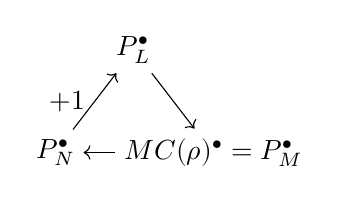
\begin{tikzpicture}[baseline=(current bounding box.center)]
    \node (L) at (1,1.3)
    {$P_L^\bullet$}; \node (N) at (0,0)
    {$P_N^\bullet$}; \node (M) at (2,0)
    {$MC(\rho)^\bullet =
      P_M^\bullet$}; \draw[->] (L) -- (M); \draw[->] (M) -- (N);
    \draw[->] (N) -- (L) node[midway, left] {$+1$};
  \end{tikzpicture}
\]
in the sense mentioned in \S{}4.1. These are the triangles giving the
homotopic category the structure of `triangulated category'. Thus, the
functor $\mathscr{P}$ allows us to construct a distinguished triangle
in $\categ{K}(\categ{P})$ starting from a `special' exact triangle
\[
  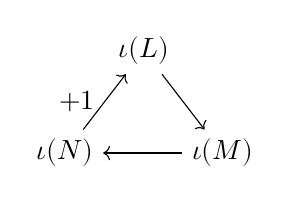
\begin{tikzpicture}[baseline=(current bounding box.center)]
    \node (L) at (1,1.3)
    {$\iota(L)$}; \node (N) at (0,0)
    {$\iota(N)$}; \node (M) at (2,0)
    {$\iota(M)$}; \draw[->] (L) -- (M); \draw[->] (M) -- (N);
    \draw[->] (N) -- (L) node[midway, left] {$+1$};
  \end{tikzpicture}
\]
in the sense of \S{}3.4. The horseshoe lemma shows that this functor
preserves as much exactness as is allowed by the context.

We should also note that once short exact sequences are lifted, we can
in fact lift every complex; this will be needed later. Here is the
precise statement:
\begin{coro}{}{coro:homol:7.9}
  Let
  \[\begin{tikzcd}[column sep=large]
      M^\bullet: & \dots \arrow[r] & M^{-3} \arrow[r] & M^{-2}
      \arrow[r] & M^{-1} \arrow[r] & M^0 \arrow[r] & 0
    \end{tikzcd}\] be a complex in an abelian category $\categ{A}$
  with enough projectives. Then there is a complex of complexes:
  \[\begin{tikzcd}[column sep=large]
      P_{M^\bullet}^\bullet: & \dots \arrow[r] & P_{M^\bullet}^{-3}
      \arrow[r] & P_{M^\bullet}^{-2} \arrow[r] & P_{M^\bullet}^{-1}
      \arrow[r] & P_{M^\bullet}^0 \arrow[r] & 0
    \end{tikzcd}\] such that each $P_{M^\bullet}^i$ is a projective
  resolution of $M^i$ and inducing $M^\bullet$ in cohomology.

  If $M^\bullet$ is exact, then $P_{M^\bullet}^\bullet$ may be chosen
  to be exact.
\end{coro}
\begin{proof}
  Break up $M^\bullet$ into short exact sequences
  \[\begin{tikzcd}
      0 \arrow[r] & K^i \arrow[r] & M^i \arrow[r] & I^{i+1} \arrow[r]
      & 0
    \end{tikzcd}\] together with exact sequences
  \[\begin{tikzcd}
      0 \arrow[r] & I^i \arrow[r] & K^i \arrow[r] & H^i \arrow[r] & 0
    \end{tikzcd}\] where $K^i$ is the kernel of $M^i \to M^{i+1}$,
  $I^{i+1}$ is its image, and $H^i$ is the cohomology at $M^i$. Choose
  arbitrary projective resolutions $P_{I^i}$, $P_{H^i}$ of $I^i$ and
  $H^i$, for all $i$. Then the horseshoe lemma
  (Lemma~\ref{lem:homol:7.8}) yields projective resolutions of $K^i$
  and short exact sequences
  \[\begin{tikzcd}
      0 \arrow[r] & P_{I^i}^\bullet \arrow[r] & P_{K^i}^\bullet
      \arrow[r] & P_{H^i}^\bullet \arrow[r] & 0,
    \end{tikzcd}\] with evident notation, and then the horseshoe lemma
  again and the previous sequences give projective resolutions
  $P_{M^i}$ of $M^i$ and short exact sequences
  \[\begin{tikzcd}
      0 \arrow[r] & P_{K^i}^\bullet \arrow[r] & P_{M^i}^\bullet
      \arrow[r] & P_{I^{i+1}}^\bullet \arrow[r] & 0.
    \end{tikzcd}\] The $P_{M^i}^\bullet$ can now be assembled into a
  sequence, by using differentials obtained by the compositions
  \[
    P_{M^i}^\bullet \to P_{I^{i+1}}^\bullet \to P_{K^{i+1}}^\bullet
    \to P_{M^{i+1}}^\bullet.
  \]
  It is clear that one obtains a complex and that
  $P_{K^{i+1}}^\bullet$, resp., $P_{I^{i+1}}^\bullet$, are the kernel,
  resp., the image, of $P_{M^i}^\bullet \to P_{M^{i+1}}^\bullet$
  (\Cref{exer:homol:1.21}). The statements follow. (If $M^\bullet$ is exact,
  then $I^i = K^i$, and the construction gives
  $P_{I^i}^\bullet = P_{K^i}^\bullet$, so that $P_{M^\bullet}^\bullet$
  is exact.)
\end{proof}

\begin{rem}{}{rem:homol:7.10}
  The proof of Corollary~\ref{coro:homol:7.9} shows that the
  resolution $P_{M^\bullet}^\bullet$, i.e.,
  \[\begin{tikzcd}[column sep=large]
      \dots \arrow[r, "d^{-4}"] & P_{M^\bullet}^{-3} \arrow[r,
      "d^{-3}"] & P_{M^\bullet}^{-2} \arrow[r, "d^{-2}"] &
      P_{M^\bullet}^{-1} \arrow[r, "d^{-1}"] & P_{M^\bullet}^0
      \arrow[r] & 0,
    \end{tikzcd}\] can in fact be chosen so that
  $\image d^i$, $\ker d^i$, and the cohomology
  $\ker d^i / \image d^{i-1}$ are all projective
  resolutions of the corresponding objects from $M^\bullet$. This is
  useful in some applications. Resolutions satisfying this property
  are called \emph{Cartan-Eilenberg} (or `fully projective')
  \emph{resolutions}.
\end{rem}

Coming back to the issue at hand, we are one step away from the
promised long exact sequence of derived functors. The last ingredient
is the following:

\begin{lem}{}{lem:homol:7.11}
  Let $\categ{A}$ be an abelian category, and let
  \[\begin{tikzcd}
      0 \arrow[r] & L^\bullet \arrow[r] & M^\bullet \arrow[r] &
      P^\bullet \arrow[r] & 0
    \end{tikzcd} \tag{$*$}\] be an exact sequence of complexes in
  $\categ{A}$, where $P^i$ is projective for all $i$. Let
  $\mathscr{F} : \categ{A} \to \categ{B}$ be any additive functor of
  abelian categories. Then the sequence obtained by applying
  $\mathscr{F}$ to $(*)$,
  \[\begin{tikzcd}
      0 \arrow[r] & \mathscr{F}(L^\bullet) \arrow[r] &
      \mathscr{F}(M^\bullet) \arrow[r] & \mathscr{F}(P^\bullet)
      \arrow[r] & 0,
    \end{tikzcd}\] is exact.
\end{lem}

Note that we are not asking $\mathscr{F}$ to be exact in any sense.

\begin{proof}
  Since $P^i$ is projective, the sequence
  \[\begin{tikzcd}
      0 \arrow[r] & L^i \arrow[r] & M^i \arrow[r] & P^i \arrow[r] & 0
    \end{tikzcd}\] splits (see the end of \ref{subsec:linrep:projectives-and-injectives}). It follows
  that
  \[\begin{tikzcd}
      0 \arrow[r] & \mathscr{F}(L^i) \arrow[r] & \mathscr{F}(M^i)
      \arrow[r] & \mathscr{F}(P^i) \arrow[r] & 0
    \end{tikzcd}\] is (split and) exact for all $i$
  (\Cref{exer:homol:5.11}). Exactness of a sequence of complexes is determined
  by exactness at each degree, so this proves the statement.
\end{proof}

Now the long exact sequence of left-derived functors is an immediate
consequence of the long exact cohomology sequence.

\begin{thm}{}{thm:homol:7.12}
  Let $\mathscr{F} : \categ{A} \to \categ{B}$ be an additive functor
  of abelian categories, and assume $\categ{A}$ has enough
  projectives. Every exact sequence
  \[\begin{tikzcd}
      0 \arrow[r] & L \arrow[r] & M \arrow[r] & N \arrow[r] & 0
    \end{tikzcd}\] in $\categ{A}$ induces a long exact sequence
  \[
    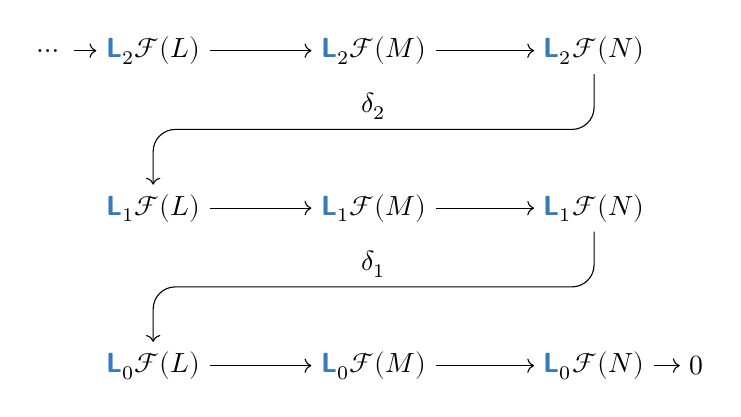
\begin{tikzpicture}[baseline=(current bounding box.center)]
      \node (dots) at (-1.3,4)
      {$\dots$}; \node (L2L) at (0,4)
      {$\categ{L}_2\mathscr{F}(L)$}; \node (L2M) at (2.8,4)
      {$\categ{L}_2\mathscr{F}(M)$}; \node (L2N) at (5.6,4)
      {$\categ{L}_2\mathscr{F}(N)$}; \node (L1L) at (0,2)
      {$\categ{L}_1\mathscr{F}(L)$}; \node (L1M) at (2.8,2)
      {$\categ{L}_1\mathscr{F}(M)$}; \node (L1N) at (5.6,2)
      {$\categ{L}_1\mathscr{F}(N)$}; \node (L0L) at (0,0)
      {$\categ{L}_0\mathscr{F}(L)$}; \node (L0M) at (2.8,0)
      {$\categ{L}_0\mathscr{F}(M)$}; \node (L0N) at (5.6,0)
      {$\categ{L}_0\mathscr{F}(N)$}; \node (zero) at (6.9,0)
      {$0$}; \draw[->] (dots) -- (L2L); \draw[->] (L2L) -- (L2M);
      \draw[->] (L2M) -- (L2N); \draw[->] (L1L) -- (L1M); \draw[->]
      (L1M) -- (L1N); \draw[->] (L0L) -- (L0M); \draw[->] (L0M) --
      (L0N); \draw[->] (L0N) -- (zero); \draw[->, rounded corners=8pt]
      (L2N.south) -- (5.6,3) -- node[above]
      {$\delta_2$} (0,3) -- (L1L.north); \draw[->, rounded
      corners=8pt] (L1N.south) -- (5.6,1) -- node[above]
      {$\delta_1$} (0,1) -- (L0L.north);
    \end{tikzpicture}
  \]
  in $\categ{B}$. Further, this assignment is covariantly functorial.
\end{thm}

The last sentence means that a morphism of short exact sequences will
induce a morphism of the corresponding long exact sequences,
compatibly with compositions. I will leave the diagram chases
necessary to prove this to the reader (\Cref{exer:homol:7.7}).

\begin{proof}
  By Lemma~\ref{lem:homol:7.8}, the given exact sequence is induced by
  an exact sequence of projective resolutions
  \[\begin{tikzcd}
      0 \arrow[r] & P_L^\bullet \arrow[r] & P_M^\bullet \arrow[r] &
      P_N^\bullet \arrow[r] & 0.
    \end{tikzcd}\] By Lemma~\ref{lem:homol:7.11}, the corresponding
  sequence
  \[\begin{tikzcd}
      0 \arrow[r] & \mathscr{F}(P_L^\bullet) \arrow[r] &
      \mathscr{F}(P_M^\bullet) \arrow[r] & \mathscr{F}(P_N^\bullet)
      \arrow[r] & 0
    \end{tikzcd}\] in $\categ{C}(\categ{B})$ is exact. As the
  cohomology objects of these complexes are precisely the left-derived
  functors of $\mathscr{F}$, the long exact cohomology sequence
  determined by this sequence (by \Cref{homol:3.5}) gives a long exact
  sequence as stated.
\end{proof}

Once more in the style of \S{}3.4, Theorem~\ref{thm:homol:7.12} tells
us that the triangle
\[
  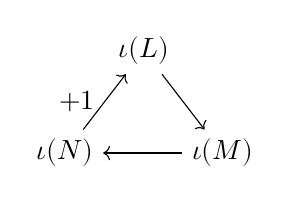
\begin{tikzpicture}[baseline=(current bounding box.center)]
    \node (L) at (1,1.3)
    {$\iota(L)$}; \node (N) at (0,0)
    {$\iota(N)$}; \node (M) at (2,0)
    {$\iota(M)$}; \draw[->] (L) -- (M); \draw[->] (M) -- (N);
    \draw[->] (N) -- (L) node[midway, left] {$+1$};
  \end{tikzpicture}
\]
induces a triangle\footnote{The indexing is potentially confusing: the
  lower $\bullet$ indicates `homological' indexing, which is opposite
  to the degree of the corresponding cochain complexes. So
  $\categ{L}_i\mathscr{F}(N)$ corresponds to degree $-i$, which is
  sent by the northeast arrow to cohomological degree $-i+1$,
  corresponding to $\categ{L}_{i-1}\mathscr{F}(L)$, as it should.}
\[
  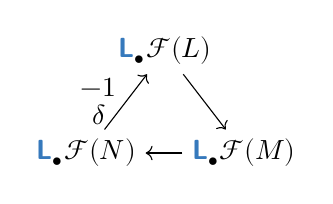
\begin{tikzpicture}[baseline=(current bounding box.center)]
    \node (L) at (1,1.3)
    {$\categ{L}_\bullet\mathscr{F}(L)$}; \node (N) at (0,0)
    {$\categ{L}_\bullet\mathscr{F}(N)$}; \node (M) at (2,0)
    {$\categ{L}_\bullet\mathscr{F}(M)$}; \draw[->] (L) -- (M);
    \draw[->] (M) -- (N); \draw[->] (N) -- (L) node[midway, left]
    {$\shortstack{$-1$ \\ $\delta$}$};
  \end{tikzpicture}
\]
The vertices of this triangle are complexes in
$\categ{C}^{\le 0} (\categ{B})$.

A completely similar situation occurs for right-derived functors: if
$\categ{A}$ has enough injectives, an exact sequence as above induces
a triangle
\[
  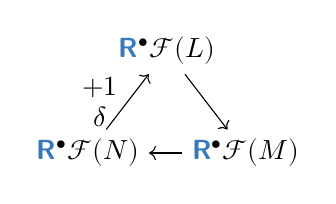
\begin{tikzpicture}[baseline=(current bounding box.center)]
    \node (L) at (1,1.3)
    {$\categ{R}^\bullet\mathscr{F}(L)$}; \node (N) at (0,0)
    {$\categ{R}^\bullet\mathscr{F}(N)$}; \node (M) at (2,0)
    {$\categ{R}^\bullet\mathscr{F}(M)$}; \draw[->] (L) -- (M);
    \draw[->] (M) -- (N); \draw[->] (N) -- (L) node[midway, left]
    {$\shortstack{$+1$ \\ $\delta$}$};
  \end{tikzpicture}
\]
where now the vertices are complexes in
$\categ{C}^{\ge 0}(\categ{B})$.

\subsection{\texorpdfstring{Relating $\mathscr{F}$,
    $\categ{L}_i\mathscr{F}$, $\categ{R}^i\mathscr{F}$}{Relating F,
    LiF, RiF}}
\label{subsec:homol:relating-f-li-f-rif}

The reader may have noticed that $\otimes$ was derived \emph{to the
  left} to obtain $\Tor$, while $\Hom$ was derived
\emph{to the right} to obtain $\operatorname{Ext}$. The asymmetry
mandating this choice lies in the fact that $\otimes$ is right-exact,
while $\Hom$ is left-exact: any additive functor can be derived to the
left or to the right (in the presence of enough projectives, resp.,
enough injectives), and the derived functors will fit in long exact
sequences as proven in Theorem~\ref{thm:homol:7.12}; but only functors
satisfying a measure of exactness can be recovered directly from their
derived versions.

To state this fact more precisely, we go back to general
considerations for the left-derived functor of an additive functor
$\mathscr{F} : \categ{A} \to \categ{B}$, where $\categ{A}$ and
$\categ{B}$ are abelian categories and $\categ{A}$ has enough
projectives, and we now assume that $\mathscr{F}$ is right-exact.

\begin{prop}{}{prop:homol:7.13}
  Let $\mathscr{F} : \categ{A} \to \categ{B}$ be a right-exact
  additive functor. Then $\categ{L}_i\mathscr{F} = 0$ for $i < 0$, and
  $\categ{L}_0\mathscr{F}$ is naturally isomorphic to $\mathscr{F}$.
\end{prop}
\begin{proof}
  Projective resolutions $P^\bullet$ of an object $M$ of $\categ{A}$
  are in $\categ{C}^{\le 0}(\categ{A})$: it follows that
  $\categ{C}(\mathscr{F})(P^\bullet)$ is $0$ in positive degree, hence
  so is its cohomology. Since $H_i = H^{-i}$ (cf. \S{}3.1), the first
  claim follows.

  As for the second, since the sequence
  \[\begin{tikzcd}
      P^{-1} \arrow[r] & P^0 \arrow[r] & M \arrow[r] & 0
    \end{tikzcd}\] is exact by construction and since $\mathscr{F}$ is
  right-exact, the sequence
  \[\begin{tikzcd}
      \mathscr{F}(P^{-1}) \arrow[r] & \mathscr{F}(P^0) \arrow[r] &
      \mathscr{F}(M) \arrow[r] & 0
    \end{tikzcd}\] is exact. This induces an isomorphism
  $\nu_L : \categ{L}_0\mathscr{F}(M) =
  H^0(\categ{C}(\mathscr{F})(P^\bullet)) \xrightarrow{\sim}
  \mathscr{F}(M)$.

  If $\varphi : M_0 \to M_1$ is a morphism in $\categ{A}$, by
  Proposition~\ref{prop:homol:6.5} there exists a morphism of
  projective resolutions
  $\alpha^\bullet : P_0^\bullet \to P_1^\bullet$ inducing $\varphi$:
  there is a commutative diagram
  \[\begin{tikzcd}
      \dots \arrow[r] & P_0^{-1} \arrow[r] \arrow[d, "\alpha^{-1}"] &
      P_0^0 \arrow[r] \arrow[d, "\alpha^0"] & M_0 \arrow[r]
      \arrow[d, "\varphi"] & 0 \\
      \dots \arrow[r] & P_1^{-1} \arrow[r] & P_1^0 \arrow[r] & M_1
      \arrow[r] & 0
    \end{tikzcd}\] and $H^0(\alpha^\bullet)$ agrees with
  $\varphi$. Applying $\mathscr{F}$ and truncating, we get a
  commutative diagram
  \[\begin{tikzcd}
      \mathscr{F}(P_0^{-1}) \arrow[r] \arrow[d,
      "\mathscr{F}(\alpha^{-1})"] & \mathscr{F}(P_0^0) \arrow[r]
      \arrow[d, "\mathscr{F}(\alpha^0)"] &
      \mathscr{F}(M_0) \arrow[r] \arrow[d, "\mathscr{F}(\varphi)"] & 0 \\
      \mathscr{F}(P_1^{-1}) \arrow[r] & \mathscr{F}(P_1^0) \arrow[r] &
      \mathscr{F}(M_1) \arrow[r] & 0
    \end{tikzcd}\] with exact rows since $\mathscr{F}$ is
  right-exact. It follows that the diagram
  \[\begin{tikzcd}
      \categ{L}_0\mathscr{F}(M_0) \arrow[r,
      "\categ{L}_0\mathscr{F}(\varphi)"] \arrow[d, "\nu_{M_0}"',
      "\sim"] & \categ{L}_0\mathscr{F}(M_1)
      \arrow[d, "\sim", "\nu_{M_1}"'] \\
      \mathscr{F}(M_0) \arrow[r, "\mathscr{F}(\varphi)"'] &
      \mathscr{F}(M_1)
    \end{tikzcd}\] commutes, proving that
  $\nu : \categ{L}_0\mathscr{F} \to \mathscr{F}$ is a natural
  isomorphism.
\end{proof}
Going back to Theorem~\ref{thm:homol:7.12}, we see that if
$\mathscr{F}$ is right-exact, then the tail end of the long exact
sequence of left-derived functors for $\mathscr{F}$ consists of an
application of $\mathscr{F}$ itself. Thus, the situation in this case
is the following: starting from a short exact sequence
\[\begin{tikzcd}
    0 \arrow[r] & L \arrow[r] & M \arrow[r] & N \arrow[r] & 0
  \end{tikzcd}\] in $\categ{A}$, we apply $\mathscr{F}$ to obtain an
exact sequence
\[\begin{tikzcd}
    \mathscr{F}(L) \arrow[r] & \mathscr{F}(M) \arrow[r] &
    \mathscr{F}(N) \arrow[r] & 0
  \end{tikzcd}\] in which we lost `the $0$ on the left'. The long
exact sequence saves the day, continuing the new sequence into an
exact complex:
\[
  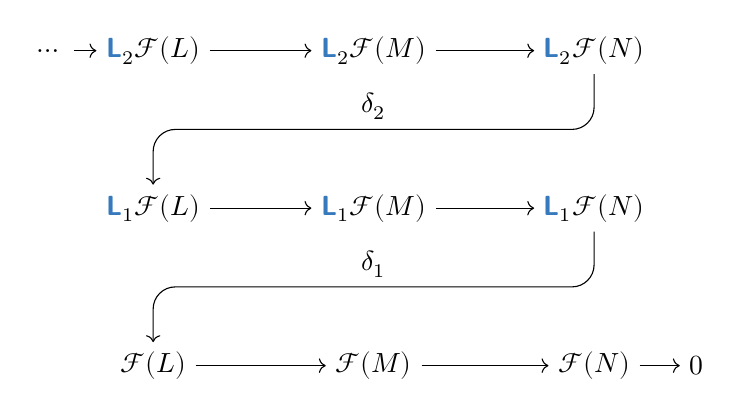
\begin{tikzpicture}[baseline=(current bounding box.center)]
    \node (dots) at (-1.3,4)
    {$\dots$}; \node (L2L) at (0,4)
    {$\categ{L}_2\mathscr{F}(L)$}; \node (L2M) at (2.8,4)
    {$\categ{L}_2\mathscr{F}(M)$}; \node (L2N) at (5.6,4)
    {$\categ{L}_2\mathscr{F}(N)$}; \node (L1L) at (0,2)
    {$\categ{L}_1\mathscr{F}(L)$}; \node (L1M) at (2.8,2)
    {$\categ{L}_1\mathscr{F}(M)$}; \node (L1N) at (5.6,2)
    {$\categ{L}_1\mathscr{F}(N)$}; \node (FL) at (0,0)
    {$\mathscr{F}(L)$}; \node (FM) at (2.8,0)
    {$\mathscr{F}(M)$}; \node (FN) at (5.6,0)
    {$\mathscr{F}(N)$}; \node (zero) at (6.9,0)
    {$0$}; \draw[->] (dots) -- (L2L); \draw[->] (L2L) -- (L2M);
    \draw[->] (L2M) -- (L2N); \draw[->] (L1L) -- (L1M); \draw[->]
    (L1M) -- (L1N); \draw[->] (FL) -- (FM); \draw[->] (FM) -- (FN);
    \draw[->] (FN) -- (zero); \draw[->, rounded corners=8pt]
    (L2N.south) -- (5.6,3) -- node[above]
    {$\delta_2$} (0,3) -- (L1L.north); \draw[->, rounded corners=8pt]
    (L1N.south) -- (5.6,1) -- node[above]
    {$\delta_1$} (0,1) -- (FL.north);
  \end{tikzpicture}
\]
That is, $\categ{L}_1\mathscr{F}$ measures the extent to which
$\mathscr{F}$ fails to be left-exact, and the higher
$\categ{L}_i\mathscr{F}$ give further measures of this failure.

Similarly, $\categ{R}^0\mathscr{F}$ is naturally isomorphic to
$\mathscr{F}$ if $\mathscr{F}$ is left-exact. In this case, applying
$\mathscr{F}$ to the original sequence gives the exact sequence
\[\begin{tikzcd}
    0 \arrow[r] & \mathscr{F}(L) \arrow[r] & \mathscr{F}(M) \arrow[r]
    & \mathscr{F}(N)
  \end{tikzcd}\] where we lost the $0$ on the right; the job of the
right-derived functors of $\mathscr{F}$ is to extend this sequence to
an exact complex
\[
  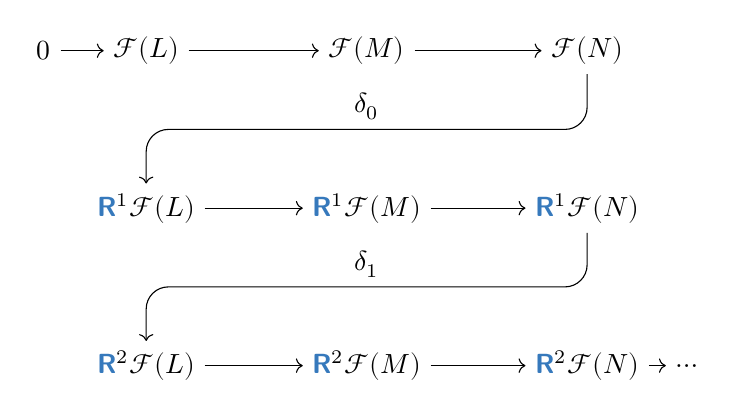
\begin{tikzpicture}[baseline=(current bounding box.center)]
    \node (zero) at (-1.3,4)
    {$0$}; \node (FL) at (0,4)
    {$\mathscr{F}(L)$}; \node (FM) at (2.8,4)
    {$\mathscr{F}(M)$}; \node (FN) at (5.6,4)
    {$\mathscr{F}(N)$}; \node (R1L) at (0,2)
    {$\categ{R}^1\mathscr{F}(L)$}; \node (R1M) at (2.8,2)
    {$\categ{R}^1\mathscr{F}(M)$}; \node (R1N) at (5.6,2)
    {$\categ{R}^1\mathscr{F}(N)$}; \node (R2L) at (0,0)
    {$\categ{R}^2\mathscr{F}(L)$}; \node (R2M) at (2.8,0)
    {$\categ{R}^2\mathscr{F}(M)$}; \node (R2N) at (5.6,0)
    {$\categ{R}^2\mathscr{F}(N)$}; \node (dots) at (6.9,0)
    {$\dots$}; \draw[->] (zero) -- (FL); \draw[->] (FL) -- (FM);
    \draw[->] (FM) -- (FN); \draw[->] (R1L) -- (R1M); \draw[->] (R1M)
    -- (R1N); \draw[->] (R2L) -- (R2M); \draw[->] (R2M) -- (R2N);
    \draw[->] (R2N) -- (dots); \draw[->, rounded corners=8pt]
    (FN.south) -- (5.6,3) -- node[above]
    {$\delta_0$} (0,3) -- (R1L.north); \draw[->, rounded corners=8pt]
    (R1N.south) -- (5.6,1) -- node[above]
    {$\delta_1$} (0,1) -- (R2L.north);
  \end{tikzpicture}
\]
No identification of $\mathscr{F}$ with any of its derived functors
should be expected if $\mathscr{F}$ does not satisfy some exactness
property. If $\mathscr{F}$ is exact on the nose, then both
$\categ{L}_0\mathscr{F}$ and $\categ{R}^0\mathscr{F}$ agree with
$\mathscr{F}$ (up to natural isomorphism); but this is no cause for
great excitement, since all other $\categ{L}_i\mathscr{F}$,
$\categ{R}^i\mathscr{F}$ vanish in this case (\Cref{exer:homol:7.8}). As
already pointed out in Example~\ref{exam:homol:7.2}, one should not
expect to learn anything new from an exact functor by deriving it.

\subsection{Example: A little group cohomology}
\label{subsec:homol:example-a-little-group-cohomology}

In the beginning of this chapter I pointed out that the general
strategy informing the development of homological algebra has numerous
applications and I mentioned group and sheaf cohomology as
examples. Here are a few words on group cohomology (sheaf cohomology
would take us too far).

How do we extract `cohomological invariants' from a group $G$?
Consider the category $G\text{-}\categ{Mod}$ of abelian groups endowed
with a left-$G$-action, equivalently, the category of
left-$\Z[G]$-modules, where $\Z[G]$ is the group ring briefly
encountered in \ref{subsec:rings:monoid-rings}. Objects of $G\text{-}\categ{Mod}$ may be
called $G$-modules.

For a $G$-module $M$, $M^G$ denotes the set of elements that are fixed
under the action of $G$: these are reasonably called the
\emph{invariants} of the action. Note that $M^G$ is an abelian group
carrying a trivial action of $G$; it is clear that setting $M \to M^G$
defines a covariant functor
$\cdot^G : G\text{-}\categ{Mod} \to \categ{Ab}$. Both
$G\text{-}\categ{Mod}$ and $\categ{Ab}$ are abelian categories, and it
takes a moment to realize that $\cdot^G$ is a left-exact functor: the
reader should either check this directly or do \Cref{exer:homol:7.16} and then
remember \Cref{linrep:1.19}. The reader should in fact contemplate why
this functor is not right-exact: if $G$ acts trivially on a coset
$[m]$ of a quotient $M/L$, there is no reason \emph{a priori} why $G$
should act trivially on a representative $m$.

We would have drawn this conclusion without difficulty before delving
into homological algebra. Homological algebra tells us how to address
this type of situation and `quantify' precisely the failure of
exactness, by means of an appropriate derived functor.

The $i$-th right-derived functor of $\cdot^G$ is denoted $H^i(G,
\_)$. Therefore, $H^0(G, M) = M^G$, and for every short exact sequence
of $G$-modules
\[\begin{tikzcd}
    0 \arrow[r] & L \arrow[r] & M \arrow[r] & N \arrow[r] & 0
  \end{tikzcd}\] we obtain (from Theorem~\ref{thm:homol:7.12}) a long
exact sequence of abelian groups:
\[\begin{tikzcd}
    0 \arrow[r] & L^G \arrow[r] & M^G \arrow[r] & N^G \arrow[r] &
    H^1(G, L) \arrow[r] & H^1(G, M) \arrow[r] & \dots
  \end{tikzcd}\] Note that $M^G = \Hom_{\Z[G]}(\Z, M)$, where $\Z$ is
given the trivial module structure. Thus,
$H^i(G, M) = \operatorname{Ext}^i_{\Z[G]}(\Z, M)$; as we know already
(and as will finally be verified in \S{}8), this can be computed by an
injective resolution of $M$ or by a projective resolution of $\Z$.
\begin{exam}{}{exam:homol:7.14}
  Take $G = \Z$. Then $\Z[G]$ is the ring $\Z[x,x^{-1}]$ of Laurent
  polynomials. As $\Z[x,x^{-1}]/(1-x) \cong \Z$, with the trivial
  action (check this!), the complex
  \[\begin{tikzcd}
      \dots \arrow[r] & 0 \arrow[r] & \Z[x,x^{-1}] \arrow[r,
      "\cdot(1-x)"] & \Z[x,x^{-1}] \arrow[r] & 0 \arrow[r] & \dots
    \end{tikzcd}\] is a free, hence projective, resolution of $\Z$,
  endowed with the trivial $\Z$-action. Applying the (contravariant)
  $\Hom_{\Z[x,x^{-1}]}(\_, M)$, we see that $H^\bullet(\Z, M)$ is
  computed by the cohomology of
  \[\begin{tikzcd}
      \dots \arrow[r] & 0 \arrow[r] & M \arrow[r, "\cdot(1-x)"] & M
      \arrow[r] & 0 \arrow[r] & \dots
    \end{tikzcd}\] `Multiplication by $x$' on $M$ is nothing but the
  action of the generator of $G = \Z$. We conclude that
  \[
    H^0(\Z, M) = \ker\bigl(M \xrightarrow{\cdot(1-x)} M\bigr) = M^{\Z}
  \]
  (as we knew already),
  \[
    H^1(\Z, M) = \frac{M}{(1-x)M},
  \]
  and $H^i(\Z, M) = 0$ for all $i < 0$ and $i \ge 2$.
\end{exam}

\begin{exam}{Finite cyclic groups}{exam:homol:7.15}
  Let $G = C_m$ be a cyclic group of order $m$; then
  $\Z[G] \cong \Z[x]/(x^m - 1)$. Again it is not difficult to produce
  a projective resolution of $\Z$ (with trivial action) in the
  category of $\Z[C_m]$-modules: letting
  $N = 1 + x + \dots + x^{m-1} = (1 - x^m)/(1 - x)$, the reader will
  verify that the complex
  \[\begin{tikzcd}
      \dots \arrow[r, "\cdot N"] & \Z[C_m] \arrow[r, "\cdot(1-x)"] &
      \Z[C_m] \arrow[r, "\cdot N"] & \Z[C_m] \arrow[r, "\cdot(1-x)"] &
      \Z[C_m] \arrow[r] & 0 \arrow[r] & \dots
    \end{tikzcd}\] has cohomology $\cong \Z$, concentrated in degree
  $0$ (i.e., on the last nonzero term). Applying
  $\Hom_{\Z[C_m]}(\_, M)$, we get the complex
  \[\begin{tikzcd}
      \dots \arrow[r] & 0 \arrow[r] & M \arrow[r, "\cdot(1-x)"] & M
      \arrow[r, "\cdot N"] & M \arrow[r, "\cdot(1-x)"] & M \arrow[r,
      "\cdot N"] & \dots
    \end{tikzcd}\] and deduce that $H^i(C_m, M) = 0$ for $i < 0$,
  $H^0(C_m, M) = M^{C_m}$, and for all $i > 0$
  \[
    H^{2i+1}(C_m, M) \cong \frac{\ker\bigl(M \xrightarrow{\cdot N}
      M\bigr)}{(1-x)M},
  \]
  \[
    H^{2i}(C_m, M) \cong \frac{M^{C_m}}{N \cdot M}.
  \]
\end{exam}
There is a standard free resolution of $\Z$ over a group ring $\Z[G]$,
which leads to a concrete description of group cohomology.  For a
finite group $G$, of order $m$, the beginning of this resolution goes
as follows. Consider the complex
\[\begin{tikzcd}[column sep=large]
    (\dagger) & \dots \arrow[r] & \Z[G]^{m^2} \arrow[r, "d^{-2}"] &
    \Z[G]^m \arrow[r, "d^{-1}"] & \Z[G] \arrow[r, "d^0"] & \Z
    \arrow[r] & 0 \arrow[r] & \dots
  \end{tikzcd}\] Here, a basis of $\Z[G]^{m^k}$ over $\Z[G]$ consists
of $k$-tuples $[g_1, \dots, g_k]$ of elements of $G$. The morphisms in
$(\dagger)$ are defined by setting
\[
  d^{-1}([g]) = 1 \cdot g - 1 \cdot e_G \in \Z[G], \qquad d^{-2}([g_1,
  g_2]) = g_1[g_2] - [g_1g_2] + [g_1],
\]
on the bases and extending by $\Z[G]$-linearity, and $d^0$ sends every
$g \in G$ to $1$, so that
$d^0\bigl(\sum_{g \in G} a_g g\bigr) = \sum_{g \in G} a_g$. (Needless
to say, $d^{-k}$ may be defined for all $k$.) The reader will check
that $(\dagger)$ is exact (\Cref{exer:homol:7.17}), at least for the part
relevant to the discussion that follows. Therefore,
\[\begin{tikzcd}[column sep=large]
    \dots \arrow[r] & \Z[G]^{m^2} \arrow[r, "d^{-2}"] & \Z[G]^m
    \arrow[r, "d^{-1}"] & \Z[G] \arrow[r] & 0 \arrow[r] & \dots
  \end{tikzcd}\] is (the beginning of) a free $\Z[G]$-resolution of
$\Z$ (endowed with the trivial $G$-action), and group cohomology can
be computed as the cohomology of the complex obtained by applying
$\Hom_{\Z[G]}(\_, M)$ to this resolution:
\[\begin{tikzcd}[column sep=large]
    0 \arrow[r] & \Hom_{\Z[G]}(\Z[G], M) \arrow[r] &
    \Hom_{\Z[G]}(\Z[G]^m, M) \arrow[r] & \Hom_{\Z[G]}(\Z[G]^{m^2}, M)
    \arrow[r] & \dots
  \end{tikzcd}\] Here, $\Hom_{\Z[G]}(\Z[G]^{m^k}, M) \cong M^{m^k}$
may be identified with the abelian group of functions $G^k \to M$,
since every $\Z[G]$-linear map $\Z[G]^{m^k} \to M$ is determined by
its action on a basis. Denote this abelian group by $C^k(G, M)$: this
is the group of $k$-cochains of $G$ with values in $M$.

We can now summarize what we have found as follows:

\begin{prop}{}{prop:homol:7.16}
  Let $G$ be a finite group, and let $M$ be a $G$-module. Then the
  group cohomology $H^i(G, M)$ is the cohomology of the cochain
  complex induced by $(\dagger)$:
  \[\begin{tikzcd}
      0 \arrow[r] & C^0(G, M) \arrow[r, "d_G^0"] & C^1(G, M) \arrow[r,
      "d_G^1"] & C^2(G, M) \arrow[r, "d_G^2"] & \dots
    \end{tikzcd}\]
\end{prop}

Tracing definitions, we see that for $a \in C^0(G, M) = M$ and
$\alpha : G \to M$ in $C^1(G, M)$,
\[
  d_G^0(a)(g) = ga - a, \qquad d_G^1(\alpha)(g_1, g_2) =
  g_1\alpha(g_2) - \alpha(g_1g_2) + \alpha(g_1).
\]
\begin{exam}{}{exam:homol:7.17}
  Let $G$ be the Galois group of a finite Galois extension
  $k \subseteq F$. Then $G$ acts on the multiplicative group $F^*$ of
  $F$, and we can view $F^*$ as a $G$-module.
\end{exam}

\begin{prop}{Hilbert's theorem 90}{prop:homol:7.18}
  $H^1(G, F^*) = 0$.
\end{prop}

Indeed, with notation as above we have
$H^1(G, F^*) \cong \ker d_G^1 / \image d_G^0$, and we can
compute this quotient explicitly. Let $\alpha \in C^1(G, F^*)$; denote
by $\alpha_g$ the image of $g$ in $F^*$ by $\alpha$. The `cocycle
condition' $\alpha \in \ker d_G^1$ translates into
\[
  \alpha_{gh} = \alpha_g \cdot g(\alpha_h)
\]
for all $g, h$ in $G$. (I am now writing the operation in $F^*$
multiplicatively and viewing elements of $G$ as automorphisms of $F$.)

The elements $h \in G$ are pairwise distinct as automorphisms of $F$,
so by \Cref{fields:exer:6.14} they must be linearly independent.  Therefore,
there exists a $\gamma \in F$ such that
\[
  \beta := \sum_{h \in G} \alpha_h \cdot h(\gamma) \ne 0.
\]
Thus $\beta \in F^*$, and for all $g \in G$
\[
  g(\beta) = \sum_{h \in G} g(\alpha_h) \cdot (gh)(\gamma)
  \overset{!}{=} \sum_{h \in G} \alpha_g^{-1} \alpha_{gh} \cdot
  (gh)(\gamma) = \alpha_g^{-1} \beta
\]
where the equality marked $\overset{!}{=}$ holds by the cocycle
condition. That is, we have found that there exists a $\beta \in F^*$
such that
\[
  \alpha_g = \frac{\beta}{g(\beta)}
\]
for all $g \in G$. But this says precisely that $\alpha$ is in the
image of $d_G^0$, proving that
$\ker d_G^1 / \image d_G^0 = 0$, as claimed.

Claim~\ref{prop:homol:7.18} is significant: it goes under the name of
\emph{Hilbert's theorem 90}, because in the case in which $G$ is the
Galois group of a finite cyclic extension, it recovers precisely the
classical result with this name. The reader had the opportunity to
prove this particular case in \Cref{fields:exer:6.16} and now will enjoy the
chance to verify that indeed Claim~\ref{prop:homol:7.18} implies
Hilbert's result (\Cref{exer:homol:7.18}).

Group cohomology is a useful tool in algebraic number theory,
algebraic topology, and other fields, and so is the companion `group
homology' $H_\bullet(G, M)$, defined analogously by the left-derived
functors of the functor $\cdot_G$ associating with every $G$-module
$M$ the module
\[
  M_G := \frac{M}{\langle gm - m \rangle_{g \in G}}
\]
(just as the elements of $M^G$ are called invariants, elements of
$M_G$ are called \emph{coinvariants} of the action). For example, in
Example~\ref{exam:homol:7.14} we verified that
$H^1(\Z, M) = M_{\Z} = H_0(\Z, M)$. The reader should now have no
difficulty computing simple examples, such as the homology
$H_\bullet(\Z, M)$ (\Cref{exer:homol:7.19}).

\subsection*{Exercises}

\begin{exer}{\exerused{}}{exer:homol:7.1}
  Let $\mathscr{T} : \categ{Ab} \to \categ{Ab}$ be the additive
  functor defined by tensoring by $\Z/2\Z$:
  $\mathscr{T}(A) := A \otimes_\Z \Z/2\Z$. Prove that no nontrivial
  projective abelian groups can be written as $\mathscr{T}(P)$, for
  any abelian group $P$. [\S{}\ref{subsec:homol:viewpoint-shift}]
\end{exer}
\begin{exer}{}{exer:homol:7.2}
  Let $\categ{A}$, $\categ{B}$ be abelian categories, let
  $\mathscr{F} : \categ{A} \to \categ{B}$ be an additive functor, and
  let
  $\categ{C}(\mathscr{F}) : \categ{C}(\categ{A}) \to
  \categ{C}(\categ{B})$ be the corresponding functor of complexes.  If
  $\alpha^\bullet : L^\bullet \to M^\bullet$ is a morphism in
  $\categ{C}(\categ{A})$, prove that $\categ{C}(\mathscr{F})$ sends
  the mapping cone of $\alpha^\bullet$ to the mapping cone of
  $\categ{C}(\mathscr{F})(\alpha^\bullet)$.
\end{exer}
\begin{exer}{\exerused{}}{exer:homol:7.3}
  With notation as in \Cref{prop:homol:7.3}, prove that the natural
  transformation
  $\categ{L}\mathscr{F} \circ \mathscr{P}_{\categ{A}} \rightsquigarrow
  \mathscr{P}_{\categ{B}} \circ \categ{K}(\mathscr{F})$ is not
  necessarily an isomorphism. (Hint: View the quasi-isomorphism in
  \Cref{homol:4.6} as a projective resolution in $\Z\text{-}\categ{Mod}$,
  and take
  $\mathscr{F} : \Z\text{-}\categ{Mod} \to
  (\Z/2\Z)\text{-}\categ{Mod}$ to be $\_\otimes_\Z (\Z/2\Z)$.)
  [\S{}\ref{subsec:homol:universal-property-of-the-derived-functor}]
\end{exer}
\begin{exer}{\exerused{}}{exer:homol:7.4}
  (Cf.\ \Cref{rem:homol:7.4}.) Let $\categ{A}$, $\categ{B}$, $\categ{C}$ be
  abelian categories, and let $\mathscr{F} : \categ{A} \to \categ{B}$,
  $\mathscr{G} : \categ{B} \to \categ{C}$ be additive functors. Assume
  that $\categ{A}$ and $\categ{B}$ have enough projectives, so that
  the derived functors $\categ{L}\mathscr{F}$ and
  $\categ{L}\mathscr{G}$ are defined, as well as the derived functor
  $\categ{L}(\mathscr{G} \circ \mathscr{F})$. Further, assume that
  $\mathscr{F}$ maps projective objects to projective objects. Prove
  that $\categ{L}\mathscr{G} \circ \categ{L}\mathscr{F}$ and
  $\categ{L}(\mathscr{G} \circ \mathscr{F})$ are naturally
  isomorphic. [\S{}\ref{subsec:homol:universal-property-of-the-derived-functor}]
\end{exer}
\begin{exer}{\exerused{}}{exer:homol:7.5}
  With notation as in \Cref{lem:homol:7.8}, show that there is a morphism
  $\rho^\bullet : P_N[-1]^\bullet \to P_L^\bullet$ such that
  $P_M^\bullet$ is homotopy equivalent to the mapping cone
  $MC(\rho)^\bullet$. (Hint: Look at the proof of the lemma; use the
  differentials $P_L^i \oplus P_N^i \to P_L^{i+1} \oplus P_N^{i+1}$ to
  define morphisms $P_N^i \to P_L^{i+1}$.) [\S{}\ref{subsec:homol:relating-f-li-f-rif}]
\end{exer}
\begin{exer}{$\lnot$}{exer:homol:7.6}
  Let $\categ{B}$, $\categ{C}$ be abelian categories, and assume
  $\categ{B}$ has enough projectives, so that Cartan-Eilenberg
  resolutions can be constructed, as in \Cref{coro:homol:7.9} (cf.\ also
  \Cref{rem:homol:7.10}). Let $\mathscr{G} : \categ{B} \to \categ{C}$ be an
  additive functor, and let
  $M^\bullet : \dots \to M^{-2} \to M^{-1} \to M^0 \to 0$ be a complex
  in $\categ{B}$. Let
  $P_{M^\bullet}^\bullet : \dots \to P_{M^\bullet}^{-2} \to
  P_{M^\bullet}^{-1} \to P_{M^\bullet}^0 \to 0$ be a Cartan-Eilenberg
  resolution of $M^\bullet$. Prove that $\mathscr{G}$ maps the
  cohomology of this complex isomorphically to the cohomology of the
  complex
  $\dots \to \mathscr{G}(P_{M^\bullet}^{-2}) \to
  \mathscr{G}(P_{M^\bullet}^{-1}) \to \mathscr{G}(P_{M^\bullet}^0) \to
  0$. (Hint: With notation as in the proof of \Cref{coro:homol:7.9}, for all
  $i$ and $j$ we have exact sequences
  $0 \to P_{K^j}^i \to P_{M^j}^i \to P_{I^{j+1}}^i \to 0$ and
  $0 \to P_{I^j}^i \to P_{K^j}^i \to P_{H^j}^i \to 0$. Note that these
  necessarily split.)

  Stenographically,
  $\mathscr{G}(H^q(P_{M^\bullet}^\bullet)) \cong
  H^q(\mathscr{G}(P_{M^\bullet}^\bullet))$, where cohomology is
  computed with respect to the $M$-degree. Also note that, by
  construction, $H^q(P_{M^\bullet}^\bullet)$ is a projective
  resolution of $H^q(M^\bullet)$; cf.\ \Cref{rem:homol:7.10}. This will be an
  ingredient in the comparison of derived functors for the composition
  of two functors by means of spectral sequences; cf.\ Exercises~8.8
  and 9.10. [\ref{exer:homol:9.10}]
\end{exer}
\begin{exer}{\exerused{}}{exer:homol:7.7}
  Complete the proof of Theorem~\ref{thm:homol:7.12} by showing that
  morphisms of short exact sequences induce morphisms of the
  corresponding long exact sequences of derived functors. [\S{}\ref{subsec:homol:long-exact-sequence-of-derived-functors}]
\end{exer}
\begin{exer}{\exerused{}}{exer:homol:7.8}
  Let $\categ{A}$, $\categ{B}$ be abelian categories, and let
  $\mathscr{F} : \categ{A} \to \categ{B}$ be an exact functor.  Assume
  $\categ{A}$ has both enough projectives and enough injectives, so
  that $\categ{L}_i\mathscr{F}$ and $\categ{R}^i\mathscr{F}$ are both
  defined. Prove that $\categ{L}_i\mathscr{F}$ and
  $\categ{R}^i\mathscr{F}$ are both the zero functor for $i \ne
  0$. [\S{}\ref{subsec:homol:relating-f-li-f-rif}]
\end{exer}
\begin{exer}{\exerused{}}{exer:homol:7.9}
  Let $\categ{A}$, $\categ{B}$ be abelian categories, and let
  $\mathscr{F} : \categ{A} \to \categ{B}$ be an additive functor.
  Assume $\categ{A}$ has enough projectives, so that
  $\categ{L}_i\mathscr{F}$ is defined. Prove that if $P$ is
  projective, then $\categ{L}_0\mathscr{F}(P) \cong \mathscr{F}(P)$
  and $\categ{L}_i\mathscr{F}(P) = 0$ for $i \ne 0$. [\S{}\ref{subsec:homol:resolution-by-acyclic-objects}]
\end{exer}
\begin{exer}{}{exer:homol:7.10}
  Let $\categ{A}$, $\categ{B}$ be abelian categories, and let
  $\mathscr{F} : \categ{A} \to \categ{B}$ be an additive functor.
  Assume $\categ{A}$ has enough projectives, so that
  $\categ{L}_i\mathscr{F}$ is defined. Prove that
  $\categ{L}_0(\mathscr{F})$ is a right-exact functor, determining the
  same higher derived functors $\categ{L}_i$, $i > 0$, as
  $\mathscr{F}$.
\end{exer}
\begin{exer}{$\lnot$}{exer:homol:7.11}
  Let $\categ{A}$, $\categ{B}$ be abelian categories, and let
  $\mathscr{F} : \categ{A} \to \categ{B}$ be an additive functor;
  assume $\categ{A}$ has enough projectives. Let
  \[\begin{tikzcd}
      0 \arrow[r] & K \arrow[r] & P \arrow[r] & A \arrow[r] & 0
    \end{tikzcd}\] be a short exact sequence in $\categ{A}$, with $P$
  projective.  Prove that
  $\categ{L}_i\mathscr{F}(A) \cong \categ{L}_{i-1}\mathscr{F}(K)$, for
  all $i > 1$. [\ref{exer:homol:7.12}]
\end{exer}
\begin{exer}{\exerused{}}{exer:homol:7.12}
  Generalize Exercise~\ref{exer:homol:7.11} as follows: with the same
  notation, assume
  \[\begin{tikzcd}
      0 \arrow[r] & K \arrow[r] & B^{-k} \arrow[r] & \dots \arrow[r] &
      B^{-1} \arrow[r] & A \arrow[r] & 0
    \end{tikzcd}\] is an exact sequence in $\categ{A}$, such that
  $\categ{L}_i\mathscr{F}(B^{-j}) = 0$ for $i > 0$, $1 \le j \le k$.
  Prove that
  $\categ{L}_i\mathscr{F}(A) \cong \categ{L}_{i-k}\mathscr{F}(K)$, for
  all $i > k$. [\S{}\ref{subsec:homol:resolution-by-acyclic-objects}, \ref{exer:homol:8.11}]
\end{exer}
\begin{exer}{$\lnot$}{exer:homol:7.13}
  Let $\categ{A}$, $\categ{B}$ be abelian categories. A collection of
  functors $\mathscr{T}^i : \categ{A} \to \categ{B}$, $i \ge 0$, is
  called a (`cohomological') $\delta$-functor if
  \begin{itemize}
  \item every short exact sequence
    \[\begin{tikzcd}
        (\dagger) & 0 \arrow[r] & L \arrow[r] & M \arrow[r] & N
        \arrow[r] & 0
      \end{tikzcd}\] in $\categ{A}$ determines `connecting morphisms'
    \[
      \delta^i : \mathscr{T}^i(N) \to \mathscr{T}^{i+1}(L)
    \]
    such that the induced sequence
    \[
      (\ddagger) \quad
      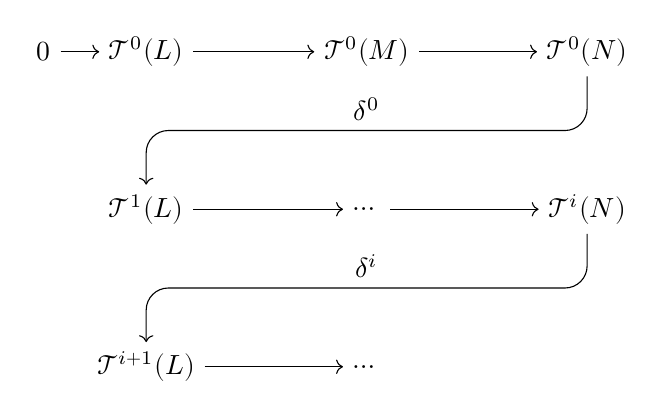
\begin{tikzpicture}[baseline=(current bounding box.center)]
        \node (zero) at (-1.3,4)
        {$0$}; \node (T0L) at (0,4)
        {$\mathscr{T}^0(L)$}; \node (T0M) at (2.8,4)
        {$\mathscr{T}^0(M)$}; \node (T0N) at (5.6,4)
        {$\mathscr{T}^0(N)$}; \node (T1L) at (0,2)
        {$\mathscr{T}^1(L)$}; \node (dots1) at (2.8,2)
        {$\dots$}; \node (TiN) at (5.6,2)
        {$\mathscr{T}^i(N)$}; \node (Ti1L) at (0,0)
        {$\mathscr{T}^{i+1}(L)$}; \node (dots2) at (2.8,0)
        {$\dots$}; \draw[->] (zero) -- (T0L); \draw[->] (T0L) --
        (T0M); \draw[->] (T0M) -- (T0N); \draw[->] (T1L) -- (dots1);
        \draw[->] (dots1) -- (TiN); \draw[->] (Ti1L) -- (dots2);
        \draw[->, rounded corners=8pt] (T0N.south) -- (5.6,3) --
        node[above]
        {$\delta^0$} (0,3) -- (T1L.north); \draw[->, rounded
        corners=8pt] (TiN.south) -- (5.6,1) -- node[above]
        {$\delta^i$} (0,1) -- (Ti1L.north);
      \end{tikzpicture}
    \]
    is exact;
  \item the assignment of a complex $(\ddagger)$ for every short exact
    sequence $(\dagger)$ is functorial (in the sense specified in
    \Cref{exer:homol:3.11}).
  \end{itemize}
  Prove that for every additive functor
  $\mathscr{F} : \categ{A} \to \categ{B}$, the derived functors
  $\categ{R}^i\mathscr{F}$, $i \ge 0$, form a cohomological
  $\delta$-functor. Prove that cohomology itself is a $\delta$-functor
  from $\categ{C}^{\ge 0}(\categ{A})$ to $\categ{A}$.

  Define a notion of `homological' $\delta$-functor
  $\{\mathscr{T}_i\}$, and prove that left-derived functors give an
  example. [\ref{exer:homol:7.14}, \ref{exer:homol:8.14}]
\end{exer}
\begin{exer}{$\lnot$}{exer:homol:7.14}
  `Morphisms' $\{\mathscr{T}^i\} \to \{\mathscr{S}^i\}$ of
  $\delta$-functors (Exercise~\ref{exer:homol:7.13}) are natural
  transformations of the individual functors $\mathscr{T}^i$,
  $\mathscr{S}^i$ that induce morphisms of the corresponding long
  exact sequences $(\ddagger)$, for every short exact sequence
  $(\dagger)$ (in other words, that preserve the connecting morphisms
  $\delta$).

  A $\delta$-functor $\{\mathscr{T}^i\}$ is \emph{universal} if for
  every $\delta$-functor $\{\mathscr{S}^i\}$, every natural
  transformation $\mathscr{T}^0 \rightsquigarrow \mathscr{S}^0$
  extends to a unique morphism of $\delta$-functors
  $\{\mathscr{T}^i\} \to \{\mathscr{S}^i\}$.

  Universal $\delta$-functors are of course unique up to isomorphism.

  It is not hard (but it involves a fair number of diagram chases) to
  show that a $\delta$-functor $\{\mathscr{T}^i\}$ is universal if for
  every $i > 0$ and every object $A$ of $\categ{A}$ there exists a
  monomorphism $\iota : A \to B$ for some $B$, such that
  $\mathscr{T}^i(\iota) = 0$. This makes each $\mathscr{T}^i$,
  $i > 0$, \emph{effaceable}. Figure out how the proof begins: assume
  that $\{\mathscr{T}^i\}$ and $\{\mathscr{S}^i\}$ are
  $\delta$-functors and that $\mathscr{T}^1$ is effaceable; show how
  to extend a natural transformation
  $\mathscr{T}^0 \rightsquigarrow \mathscr{S}^0$ to a natural
  transformation $\mathscr{T}^1 \rightsquigarrow \mathscr{S}^1$,
  compatibly with the connecting morphisms. (Hint: If $\mathscr{T}^1$
  is effaced by $\iota : A \to B$, let $C = \coker\iota$
  and consider the exact sequence $0 \to A \to B \to C \to 0$.) [\ref{exer:homol:7.15}]
\end{exer}
\begin{exer}{$\lnot$}{exer:homol:7.15}
  Assume the result stated in Exercise~\ref{exer:homol:7.14}. Prove
  that right-derived functors are universal cohomological
  $\delta$-functors. (Equivalently, left-derived functors are
  universal homological $\delta$-functors.) For an abelian category
  $\categ{A}$, Prove that cohomology, viewed as a collection of
  functors from $\categ{C}^{\ge 0}(\categ{A})$ to $\categ{A}$, is a
  universal $\delta$-functor. (Hint: To efface
  $\categ{R}^i\mathscr{F}$ for $i > 0$, use injectives. To efface
  $H^i$ for $i > 0$, stare at the sequence of complexes mentioned
  right before the statement of \Cref{homol:4.1}.)

  The upshot is that in order to verify that a given collection of
  functors agrees with the derived functors of a given (say)
  left-exact functor, it suffices to verify that they form a
  cohomological $\delta$-functor and that the effaceability condition
  holds. This is used, for example, to obtain concrete realizations of
  sheaf cohomology. [\ref{exer:homol:8.14}]
\end{exer}
\begin{exer}{\exerused{}}{exer:homol:7.16}
  Prove that the functor $\cdot^G$ defined in \S{}7.6 is right-adjoint
  to the functor $\categ{Ab} \to G\text{-}\categ{Mod}$ associating
  with an abelian group $A$ the same group, endowed with the trivial
  $G$-action. Give an analogous interpretation for the functor
  $\cdot_G$. [\S{}\ref{subsec:homol:example-a-little-group-cohomology}]
\end{exer}
\begin{exer}{\exerused{}}{exer:homol:7.17}
  Consider the complex $(\dagger)$ defined in \S{}7.6. Define maps
  $h^{-1}$, $h^0$, $h$ in the diagram
  \[\begin{tikzcd}[column sep=large]
      \dots \arrow[r] & \Z[G]^{m^2} \arrow[r, "d^{-2}"] & \Z[G]^m
      \arrow[r, "d^{-1}"] \arrow[dl, dashed, "h^{-1}"'] & \Z[G]
      \arrow[r, "d^0"] \arrow[dl, dashed, "h^0"'] & \Z \arrow[r]
      \arrow[dl, dashed, "h"'] & 0 \arrow[r] & \dots \\
      \dots \arrow[r] & \Z[G]^{m^2} \arrow[r, "d^{-2}"] & \Z[G]^m
      \arrow[r, "d^{-1}"] & \Z[G] \arrow[r, "d^0"] & \Z \arrow[r] & 0
      \arrow[r] & \dots
    \end{tikzcd}\] by
  \[
    h(a) := a \cdot e_G, \qquad h^0(g) := [g], \qquad h^{-1}([g]) :=
    [e_G, g]
  \]
  (and extending by $\Z[G]$-linearity). Use these maps to verify that
  the complex $(\dagger)$ is exact at $\Z$, $\Z[G]$,
  $\Z[G]^m$. [\S{}\ref{subsec:homol:example-a-little-group-cohomology}]
\end{exer}
\begin{exer}{\exerused{}}{exer:homol:7.18}
  Deduce Hilbert's theorem 90 (as stated in \Cref{fields:exer:6.16}) as a
  consequence of the vanishing of Claim~\ref{prop:homol:7.18}.  (Hint:
  Use the result of Example~\ref{exam:homol:7.15}.) [\S{}\ref{subsec:homol:example-a-little-group-cohomology}]
\end{exer}
\begin{exer}{\exerused{}}{exer:homol:7.19}
  Compute the group homology $H_\bullet(\Z, M)$ for any abelian group
  $M$ carrying a $\Z$-action. [\S{}\ref{subsec:homol:example-a-little-group-cohomology}]
\end{exer}

\section{Double complexes}
\label{sec:homol:double-complexes}

A few mysteries remain on the table concerning Tor and Ext: the fact
that, e.g., \emph{flat} resolutions may be used in place of projective
ones in order to compute Tor and the fact that resolving `either
argument' leads to the same functors. For example,
$\operatorname{Ext}^i_R(M, N)$ may be computed by using a projective
resolution of $M$ or an injective resolution of $N$.

Both mysteries are (of course) instances of general features of the
theory, which we examine in this section. The first can be dispelled
with a pleasant inductive argument that seems worth presenting
(\S{}8.1). But everything is clarified substantially by going one step
further and considering \emph{double complexes}, as we do in the
remaining subsections.

\subsection{Resolution by acyclic objects}
\label{subsec:homol:resolution-by-acyclic-objects}

Let $\categ{A}$ be an abelian category with enough projectives, and
let $\mathscr{F} : \categ{A} \to \categ{B}$ be an additive functor to
another abelian category. At this point we know how to construct
left-derived functors
$\categ{L}_i\mathscr{F} : \categ{A} \to \categ{B}$ of $\mathscr{F}$:
in two words, $\categ{L}_i\mathscr{F}(M)$ is computed by applying
$\mathscr{F}$ to a projective resolution of $M$ and taking
(co)homology of the resulting complex.

It follows in particular that $\categ{L}_i\mathscr{F}(P) = 0$ for
$i \ge 1$ if $P$ is projective (cf.\ Exercise~\ref{exer:homol:7.9}):
if $P$ is projective, then $\iota(P)$:
\[\begin{tikzcd}
    \dots \arrow[r] & 0 \arrow[r] & 0 \arrow[r] & P \arrow[r] & 0
    \arrow[r] & \dots
  \end{tikzcd}\] is a projective resolution of $P$, so
$\categ{L}_\bullet\mathscr{F}(P)$ is the cohomology of
\[\begin{tikzcd}
    \dots \arrow[r] & 0 \arrow[r] & 0 \arrow[r] & \mathscr{F}(P)
    \arrow[r] & 0 \arrow[r] & \dots
  \end{tikzcd}\] that is,
\[
  \categ{L}_i\mathscr{F}(P) =
  \begin{cases}
    \mathscr{F}(P), & i = 0, \\
    0, & i \ne 0.
  \end{cases}
\]
This says that projective objects are `$\mathscr{F}$-acyclic' with
respect to left-derived functors:

\begin{defn}{}{defn:homol:8.1}
  Let $\mathscr{F}$ be an additive functor. An object $M$ of
  $\categ{A}$ is \emph{$\mathscr{F}$-acyclic} (w.r.t.\ left-derived
  functors) if $\categ{L}_i\mathscr{F}(M) = 0$ for $i \ne 0$.
\end{defn}

An object $M$ is $\mathscr{F}$-acyclic with respect to right-derived
functors if $\categ{R}^i\mathscr{F}(M) = 0$ for $i \ne 0$. In
practice, this notion is really useful only for right-exact or
left-exact functors; the first are derived on the left, and the second
on the right (cf.\ \S{}7.5), so in context we can just talk about
`$\mathscr{F}$-acyclic' objects.

While projectives are acyclic for every right-exact functor, a given
functor $\mathscr{F}$ may admit other $\mathscr{F}$-acyclic objects.

\begin{exam}{}{exam:homol:8.2}
  Let $R$ be a commutative ring. Recall (\Cref{linrep:2.13}) that an
  $R$-module $M$ is \emph{flat} if $\_ \otimes_R M$ is exact, or
  equivalently (by the symmetry of $\otimes$) if $M \otimes_R \_$ is
  exact. Flat modules are acyclic with respect to tensor products, in
  a very strong sense: if $N$ is flat, then
  $\Tor_i(M, N) = 0$ for $i \ne 0$ and all $M$; see
  \ref{subsec:linrep:the-tor-functors} to be reminded of why, or---better---prove it anew.
  Further, since (as we will finally prove in this section) Tor
  functors may be computed by resolving either argument, we also know
  that, `symmetrically', if $M$ is flat, then
  $\Tor_i(M, N) = 0$ for all $i \ne 0$ and all modules
  $N$. Thus, a flat module is $\mathscr{F}$-acyclic for every functor
  $\mathscr{F}$ defined by $\_ \otimes_R N$, for all modules $N$.
\end{exam}

Here is the punch line. In \ref{subsec:linrep:the-ext-functors} I had claimed that flat
resolutions could be used in place of free or projective resolutions,
in order to compute Tor. We are going to verify that
$\mathscr{F}$-acyclic resolutions suffice in order to compute
$\categ{L}_i\mathscr{F}$.

\begin{thm}{}{thm:homol:8.3}
  Let $\mathscr{F} : \categ{A} \to \categ{B}$ be a right-exact functor
  of abelian categories, and assume $\categ{A}$ has enough
  projectives. Let
  \[\begin{tikzcd}
      A^\bullet : & \dots \arrow[r] & A^{-2} \arrow[r, "d_A^{-2}"] &
      A^{-1} \arrow[r, "d_A^{-1}"] & A^0 \arrow[r] & 0 \arrow[r] &
      \dots
    \end{tikzcd}\] be a resolution of an object $M$ of $\categ{A}$,
  such that every object $A^i$ is $\mathscr{F}$-acyclic. Then for all
  $i$
  \[
    \categ{L}_i\mathscr{F}(M) \cong
    H^{-i}(\categ{C}(\mathscr{F})(A^\bullet)).
  \]
  If the objects $A^i$ are projective, the statement is the very
  definition of $\categ{L}_i\mathscr{F}$. The theorem states that
  $\mathscr{F}$-acyclic objects may be used in place of projective
  objects in the computation of $\categ{L}_i\mathscr{F}$.
\end{thm}
\begin{proof}
  The first two cases follow from explicit computations. To begin
  with, the sequence
  \[\begin{tikzcd}
      A^{-1} \arrow[r] & A^0 \arrow[r] & M \arrow[r] & 0
    \end{tikzcd}\] is exact by assumption, and $\mathscr{F}$ is
  right-exact; thus
  \[\begin{tikzcd}
      \mathscr{F}(A^{-1}) \arrow[r] & \mathscr{F}(A^0) \arrow[r] &
      \mathscr{F}(M) \arrow[r] & 0
    \end{tikzcd}\] is exact, and it follows that
  \[
    H^0(\categ{C}(\mathscr{F})(A^\bullet)) \cong \mathscr{F}(M) \cong
    \categ{L}_0\mathscr{F}(M).
  \]
  Next, let $K$ be the kernel of $A^0 \to M$; so we have the short
  exact sequence
  \[
    (*) \qquad
    \begin{tikzcd}
      0 \arrow[r] & K \arrow[r] & A^0 \arrow[r] & M \arrow[r] & 0
    \end{tikzcd}
  \]
  Applying Theorem~\ref{thm:homol:7.12} (and
  Proposition~\ref{prop:homol:7.13}), we obtain a long exact sequence
  ending with
  \[\begin{tikzcd}
      \categ{L}_1\mathscr{F}(A^0) \arrow[r] &
      \categ{L}_1\mathscr{F}(M) \arrow[r] & \mathscr{F}(K) \arrow[r] &
      \mathscr{F}(A^0) \arrow[r] & \mathscr{F}(M) \arrow[r] & 0
    \end{tikzcd}\] The leftmost term is $0$ since $A^0$ is
  $\mathscr{F}$-acyclic. It follows that
  \[
    \categ{L}_1\mathscr{F}(M) \cong \ker(\mathscr{F}(K) \to
    \mathscr{F}(A^0)) \cong H^{-1}(\categ{C}(\mathscr{F})(A^\bullet)):
  \]
  for the second $\cong$, apply the result of (the straightforward)
  \Cref{exer:homol:8.1} to the exact complex
  \[\begin{tikzcd}
      \dots \arrow[r] & A^{-1} \arrow[r] & A^0 \arrow[r] & M \arrow[r]
      & 0 \arrow[r] & \dots
    \end{tikzcd}\] Finally, use induction on $i$. We have just
  verified that the theorem holds for all objects $M$ and for
  $i = 0, 1$; given $i > 1$, assume the statement is known for all
  objects of $\categ{A}$ and all indices $< i$. Truncating/shifting
  $A^\bullet$,
  \[\begin{tikzcd}
      \dots \arrow[r] & A^{-3} \arrow[r] & A^{-2} \arrow[r] & A^{-1}
      \arrow[r] & 0 \arrow[r] & \dots
    \end{tikzcd}\] (so that $A^{-1}$ is placed in degree $0$), gives
  an $\mathscr{F}$-acyclic resolution of $K$; by the induction
  hypothesis, $\categ{L}_{i-1}\mathscr{F}(K)$ may be computed by
  applying $\categ{C}(\mathscr{F})$ to this complex and taking
  cohomology:
  \[
    \categ{L}_{i-1}\mathscr{F}(K) \cong
    H^{-i}(\categ{C}(\mathscr{F})(A^\bullet)).
  \]
  On the other hand, the other terms in the long exact sequence
  obtained by applying Theorem~\ref{thm:homol:7.12} to $(*)$ give
  \[\begin{tikzcd}
      \dots \arrow[r] & \categ{L}_i\mathscr{F}(A^0) \arrow[r] &
      \categ{L}_i\mathscr{F}(M) \arrow[r] &
      \categ{L}_{i-1}\mathscr{F}(K) \arrow[r] &
      \categ{L}_{i-1}\mathscr{F}(A^0) \arrow[r] & \dots
    \end{tikzcd}\] since $A^0$ is $\mathscr{F}$-acyclic and $i > 1$,
  this shows that
  \[
    \categ{L}_i\mathscr{F}(M) \cong \categ{L}_{i-1}\mathscr{F}(K)
  \]
  (also cf.\ Exercise~\ref{exer:homol:7.12}) and concludes the proof.
\end{proof}

\begin{exam}{}{exam:homol:8.4}
  Let $R$ be a commutative ring, and let
  \[\begin{tikzcd}
      F_\bullet : & \dots \arrow[r] & F_2 \arrow[r] & F_1 \arrow[r] &
      F_0 \arrow[r] & 0
    \end{tikzcd}\] be a resolution of an $R$-module $M$ by flat
  $R$-modules. Then for every $R$-module $N$,
  \[
    \Tor^R_i(M, N) \cong H_i(F_\bullet \otimes_R N).
  \]
  Indeed, flat modules are acyclic with respect to $\_ \otimes N$
  (Example~\ref{exam:homol:8.2}), so this is now a consequence of
  Theorem~\ref{thm:homol:8.3}.
\end{exam}

Theorem~\ref{thm:homol:8.3} raises an interesting possibility: since
$\mathscr{F}$-acyclic objects suffice in order to compute the derived
functors of $\mathscr{F}$ (at least when $\mathscr{F}$ is
right-exact), the reader can imagine that there may be situations in
which $\categ{A}$ does \emph{not} have enough projectives, and yet
left-derived functors of a functor $\mathscr{F}$ may be defined
because $\categ{A}$ has enough $\mathscr{F}$-acyclic objects (in a
suitable sense). This is indeed the case. The reader will run into
such examples in more advanced treatments of the subject. (See
\Cref{exer:homol:8.14} for a typical situation.)

There is an alternative viewpoint on the question addressed by
Theorem~\ref{thm:homol:8.3}. Let $A^\bullet$ be an
$\mathscr{F}$-acyclic resolution of an object $M$, and let
$P_M^\bullet$ be a projective resolution. I will apply
$\categ{C}(\mathscr{F})$ and place the resulting complexes as sides of
an array:
\[\begin{tikzcd}[column sep=small]
    \dots \arrow[r] & \mathscr{F}(A^{-2}) \arrow[r] &
    \mathscr{F}(A^{-1})
    \arrow[r] & \mathscr{F}(A^0) \arrow[r] & \mathscr{F}(M) \\
    {} & & & & \mathscr{F}(P_M^0) \arrow[u] \\
    {} & & & & \mathscr{F}(P_M^{-1}) \arrow[u] \\
    {} & & & & \mathscr{F}(P_M^{-2}) \arrow[u] \\
    & & & & \vdots \arrow[u] \arrow[dotted, from=2-1, to=2-5]
    \arrow[dotted, from=3-1, to=3-5] \arrow[dotted, from=4-1, to=4-5]
  \end{tikzcd}\] The result of Theorem~\ref{thm:homol:8.3} is that
taking cohomology of the top row of this diagram gives the same result
as taking cohomology of the rightmost column. Might there not be a way
to `interpolate' between these two cohomologies, by cleverly filling
in the dotted portion of this diagram?

\emph{Double complexes} may be used to this effect, as we will see in
a moment.

\subsection{Complexes of complexes}
\label{subsec:homol:complexes-of-complexes}

I warned the reader as far back as \S{}3.2 that we would examine
complexes \emph{of complexes}, that is, objects of
$\categ{C}(\categ{C}(\categ{A}))$, for an abelian category
$\categ{A}$. We have run across particular cases: the exact sequences
of complexes leading to the long exact cohomology sequence (\S{}3.3)
and the construction of the mapping cone (\S{}4.1). The latter case
generalizes in a straightforward way, as we will see now.

Keeping with the tradition established earlier in the chapter, I will
concentrate on the `bounded-above' case; the reader should have no
difficulty reproducing the bounded-below version of what we will do
and should be aware of the fact that the material can be developed to
a large extent without boundedness conditions.

An object of $\categ{C}^{\le 0}(\categ{C}^{\le 0}(\categ{A}))$ is a
complex
\[\begin{tikzcd}
    \dots \arrow[r] & M^{-3,\bullet} \arrow[r, "d_h^{-3,\bullet}"] &
    M^{-2,\bullet} \arrow[r, "d_h^{-2,\bullet}"] & M^{-1,\bullet}
    \arrow[r, "d_h^{-1,\bullet}"] & M^{0,\bullet} \arrow[r] & 0
    \arrow[r] & \dots
  \end{tikzcd}\] in which the object $M^{i,\bullet}$ in degree $i$ is
itself a complex in $\categ{C}^{\le 0}(\categ{A})$. The subscript $h$
stands, rather unimaginatively, for `horizontal'; we have
$d_h^{i,\bullet} \circ d_h^{i-1,\bullet} = 0$. An example that will
motivate the next construction is the particular case in which only
two objects are nonzero:
\[
  (*) \qquad
  \begin{tikzcd}
    \dots \arrow[r] & 0 \arrow[r] & 0 \arrow[r] & L^\bullet \arrow[r,
    "\alpha^\bullet"] & M^\bullet \arrow[r] & 0 \arrow[r] & \dots
  \end{tikzcd}
\]
(and we are considering the particular case in which $L^\bullet$,
$M^\bullet$ are bounded above). I will (arbitrarily) place $M^\bullet$
in degree $0$ and $L^\bullet$ in degree $-1$. We can view the
information carried by $(*)$ as a commutative diagram:
\[\begin{tikzcd}
    & \vdots \arrow[d, "d_L^{i+1}"] & & \vdots \arrow[d, "d_M^{i+1}"] & \\
    \dots \arrow[r] & 0 \arrow[r] & L^{i+1} \arrow[r, "\alpha^{i+1}"]
    \arrow[d, "d_L^i"'] & M^{i+1} \arrow[r] \arrow[d, "d_M^i"'] & 0
    \arrow[r] & \dots \\
    \dots \arrow[r] & 0 \arrow[r] & L^i \arrow[r, "\alpha^i"]
    \arrow[d, "d_L^{i-1}"'] & M^i \arrow[r] \arrow[d, "d_M^{i-1}"'] &
    0 \arrow[r]
    & \dots \\
    \dots \arrow[r] & 0 \arrow[r] & L^{i-1} \arrow[r, "\alpha^{i-1}"]
    \arrow[d] & M^{i-1} \arrow[r] \arrow[d] & 0 \arrow[r] & \dots \\
    & & \vdots & \vdots &
  \end{tikzcd}\]

The mapping cone $MC(\alpha)^\bullet$ constructed in \S{}4.1 is
obtained by
\begin{itemize}
\item shifting the complex in degree $-i$ by $i$,
\item direct-summing the rows and morphisms of the resulting diagram,
  collapsing it to a single vertical complex:
\end{itemize}
% TODO: diagram of the shifted, anticommutative version of the ladder
% diagram above (source page 666), showing the columns collapsed
% row-by-row into direct sums L^i \oplus M^{i-1}, with diagonal arrows
% \alpha^{i+1}, d_{M^\bullet}^i and dotted diagonal arrows
% illustrating the direct-summing step; purely a pedagogical picture
% of the mapping-cone construction already defined algebraically in
% \S{}4.1, no new mathematical content beyond what the surrounding
% prose states.

Note that, due to the shift, the diagram on the left has become
\emph{anti}commutative in the process. The extra signs are necessary
in order that $MC(\alpha)^\bullet$ be a complex.

Now we will apply the same procedure to the more general case
\[\begin{tikzcd}
    \dots \arrow[r] & M^{-3,\bullet} \arrow[r, "d_h^{-3,\bullet}"] &
    M^{-2,\bullet} \arrow[r, "d_h^{-2,\bullet}"] & M^{-1,\bullet}
    \arrow[r, "d_h^{-1,\bullet}"] & M^{0,\bullet} \arrow[r] & 0
    \arrow[r] & \dots
  \end{tikzcd}\] This corresponds to the commutative diagram
\[\begin{tikzcd}
    \dots & M^{-3,0} \arrow[r, "d_h"] \arrow[d, "d_v"'] & M^{-2,0}
    \arrow[r, "d_h"] \arrow[d, "d_v"'] & M^{-1,0} \arrow[r, "d_h"]
    \arrow[d, "d_v"'] & M^{0,0} \arrow[d, "d_v"'] \\
    \dots & M^{-3,-1} \arrow[r, "d_h"] \arrow[d, "d_v"'] & M^{-2,-1}
    \arrow[r, "d_h"] \arrow[d, "d_v"'] & M^{-1,-1} \arrow[r, "d_h"]
    \arrow[d, "d_v"'] & M^{0,-1} \arrow[d, "d_v"'] \\
    \dots & M^{-3,-2} \arrow[r, "d_h"] \arrow[d] & M^{-2,-2} \arrow[r,
    "d_h"] \arrow[d] & M^{-1,-2} \arrow[r, "d_h"] \arrow[d] & M^{0,-2}
    \arrow[d] \\
    \dots & \vdots & \vdots & \vdots & \vdots
  \end{tikzcd}\] surrounded by $0$ above and to the right (omitted
here not to clutter the diagram; the upper indices of the
differentials are sacrificed for the same reason); the subscript $v$
stands for `vertical'. As above, we shift $M^{-i,\bullet}$ by $i$,
with the effect of changing the sign of the differentials in the
odd-shifted columns; I will let $\delta_v$ denote $d_v$ on even-degree
columns and $-d_v$ on odd-degree columns. The resulting diagram is
anticommutative:
% TODO: diagram of the staggered (anticommutative) version of the grid
% diagram above (source page 667), with columns offset vertically in a
% staircase arrangement to visually convey the degree shift, labeled
% with alternating d_h/\delta_v arrows; a pedagogical restaging of the
% preceding grid, no new mathematical content beyond the sign
% convention already stated in the surrounding prose.

Taking direct sums of the objects and morphisms on each row, as in the
case of the mapping cone, determines a new complex, called the
\emph{total complex} $TC(M)^\bullet$ of the given complex of
complexes.

\emph{Double complexes} capture this construction:

\begin{defn}{}{defn:homol:8.5}
  A \emph{double (cochain) complex} on an abelian category $\categ{A}$
  is an array of objects $M^{i,j}$ of $\categ{A}$, $i, j \in \Z$,
  endowed with morphisms
  \[
    d_h^{i,j} : M^{i,j} \to M^{i+1,j}, \qquad \delta_v^{i,j} : M^{i,j}
    \to M^{i,j+1}
  \]
  such that
  \[
    \begin{cases}
      d_h^{i,j} \circ d_h^{i-1,j} = 0, \\
      \delta_v^{i,j} \circ \delta_v^{i,j-1} = 0, \\
      \delta_v^{i+1,j} \circ d_h^{i,j} + d_h^{i,j+1} \circ
      \delta_v^{i,j} = 0.
    \end{cases}
  \]
\end{defn}

That is, the columns $M^{i,\bullet}$ and the rows $M^{\bullet,j}$ both
form complexes, and the whole diagram \emph{anticommutes}.  Dropping
the position specification, the conditions defining a double complex
are summarized in the easier-to-parse prescription
\[
  \begin{cases}
    d_h \circ d_h = 0, \\
    \delta_v \circ \delta_v = 0, \\
    \delta_v \circ d_h + d_h \circ \delta_v = 0.
  \end{cases}
\]

Double complexes, with or without appropriate boundedness conditions
(such as requiring $M^{i,j} = 0$ for $i > 0$, $j > 0$, as in the case
considered above), form a category in an evident way. It is equally
evident that this category is equivalent to the correspondingly
bounded category of complexes of complexes: every object of
$\categ{C}^{\le 0}(\categ{C}^{\le 0}(\categ{A}))$ determines a double
complex by setting $\delta_v^{i,j} = (-1)^i d_v^{i,j}$, as
above. Changing the signs of odd \emph{rows} rather than columns leads
to an isomorphic double complex, \Cref{exer:homol:8.4}; in fact, other choices
may be convenient depending on the situation.

From this viewpoint, the total complex $TC(M)^\bullet$ (also called
the \emph{simple} of the double complex $M^{\bullet,\bullet}$) is
obtained by direct-summing objects and morphisms of the double complex
along diagonals:
% TODO: diagram of the total-complex-along-diagonals construction
% (source page 668): the staggered grid of M^{i,j} terms shown
% alongside a right-hand column of direct sums (e.g. M^{-2,0} \oplus
% M^{-1,-1} \oplus M^{0,-2}) with dotted diagonal lines grouping the
% terms on each antidiagonal i+j=k into the corresponding TC(M)^k;
% purely illustrates Definition~8.6 below, no separate mathematical
% content.

\begin{defn}{}{defn:homol:8.6}
  The \emph{total complex} $TC(M)^\bullet$ of a double complex
  $M^{\bullet,\bullet}$ is defined by setting
  $TC(M)^k := \bigoplus_{i+j=k} M^{i,j}$, with differentials (written
  stenographically) $d_{tot} = d_h + \delta_v$.
\end{defn}

\begin{prop}{}{prop:homol:8.7}
  $(TC(M)^\bullet, d_{tot}^\bullet)$ is indeed a complex.
\end{prop}
\begin{proof}
  The question is whether the composition of two consecutive
  differentials vanishes, as it should. Insisting with our shorthand,
  \[
    d_{tot} \circ d_{tot} = (d_h + \delta_v) \circ (d_h + \delta_v) =
    d_h \circ d_h + d_h \circ \delta_v + \delta_v \circ d_h + \delta_v
    \circ \delta_v = 0.
  \]
  The reader will formalize this computation (\Cref{exer:homol:8.3}).
\end{proof}

It is clear from the definition that $TC(M)^\bullet$ agrees with the
mapping cone, when $M^{\bullet,\bullet}$ is concentrated in degrees
$-1$ and $0$.

The total complex is defined even without any boundedness hypothesis,
but then one has to choose whether to use direct \emph{sums} or direct
\emph{products} as objects of the complex.  Since only bounded
complexes will be needed in the applications we will see, I will
happily leave such complications aside and limit the discussion to the
bounded case.

\begin{exam}{}{exam:homol:8.8}
  Operations such as $\Hom_{\categ{A}}$ or $\otimes$ determine double
  complexes. For a `first quadrant' example, let $L^\bullet$, resp.,
  $M^\bullet$, be a complex in $\categ{C}^{\le 0}(\categ{A})$, resp.\
  $\categ{C}^{\ge 0}(\categ{A})$:
  \[\begin{tikzcd}
      \dots \arrow[r] & L^{-2} \arrow[r] & L^{-1} \arrow[r] & L^0
      \arrow[r] & 0 \arrow[r] & \dots
    \end{tikzcd}\]
  \[\begin{tikzcd}
      \dots \arrow[r] & 0 \arrow[r] & M^0 \arrow[r] & M^1 \arrow[r] &
      M^2 \arrow[r] & \dots
    \end{tikzcd}\] We can consider the complex in
  $\categ{C}^{\ge 0}(\categ{C}^{\ge 0})$:
  \[\begin{tikzcd}
      \dots \arrow[r] & 0 \arrow[r] & \Hom_{\categ{A}}(L^\bullet, M^0)
      \arrow[r] & \Hom_{\categ{A}}(L^\bullet, M^1) \arrow[r] &
      \Hom_{\categ{A}}(L^\bullet, M^2) \arrow[r] & \dots
    \end{tikzcd}\] that is, in `grid' form (and omitting zeros to the
  left and below):
  \[\begin{tikzcd}
      \vdots \arrow[d] & \vdots \arrow[d] & \vdots \arrow[d] & \\
      \Hom_{\categ{A}}(L^{-2}, M^0) \arrow[r] &
      \Hom_{\categ{A}}(L^{-2},
      M^1) \arrow[r] & \Hom_{\categ{A}}(L^{-2}, M^2) \arrow[r] & \dots \\
      \Hom_{\categ{A}}(L^{-1}, M^0) \arrow[r] \arrow[u] &
      \Hom_{\categ{A}}(L^{-1}, M^1) \arrow[r] \arrow[u] &
      \Hom_{\categ{A}}(L^{-1}, M^2) \arrow[r] \arrow[u] & \dots \\
      \Hom_{\categ{A}}(L^0, M^0) \arrow[r] \arrow[u] &
      \Hom_{\categ{A}}(L^0, M^1) \arrow[r] \arrow[u] &
      \Hom_{\categ{A}}(L^0, M^2) \arrow[r] \arrow[u] & \dots
    \end{tikzcd}\]

  We could also consider the complex of complexes
  \[\begin{tikzcd}
      \dots \arrow[r] & 0 \arrow[r] & \Hom_{\categ{A}}(L^0, M^\bullet)
      \arrow[r] & \Hom_{\categ{A}}(L^{-1}, M^\bullet) \arrow[r] &
      \Hom_{\categ{A}}(L^{-2}, M^\bullet) \arrow[r] & \dots
    \end{tikzcd}\] and this would lead to the grid obtained by
  flipping the previous one about the main diagonal. The two
  corresponding total complexes are then clearly isomorphic
  (\Cref{exer:homol:8.4}), and by a slight abuse of language they can both be
  denoted $TC(\Hom_{\categ{A}}(L, M))^\bullet$. The degree-$i$ piece
  of this total complex, i.e.,
  \[
    \Hom_{\categ{A}}(L^{-i}, M^0) \oplus \Hom_{\categ{A}}(L^{-i+1},
    M^1) \oplus \dots \oplus \Hom_{\categ{A}}(L^0, M^i),
  \]
  parametrizes degree-preserving morphisms from objects of $L^\bullet$
  to objects of $M[i]^\bullet$. These are not cochain morphisms
  $L^\bullet \to M[i]^\bullet$, since the corresponding diagrams
  \[\begin{tikzcd}
      \dots \arrow[r] & 0 \arrow[r] & M[i]^{-i} \arrow[r] &
      M[i]^{-i+1} \arrow[r] & \dots \arrow[r] & M[i]^0 \arrow[r] &
      \dots \\
      \dots \arrow[r] & L^{-i-1} \arrow[r] \arrow[u] & L^{-i}
      \arrow[r] & L^{-i+1} \arrow[r] & \dots \arrow[r] & L^0 \arrow[r]
      & 0 \arrow[r] & \dots
    \end{tikzcd}\] do not satisfy any commutativity hypothesis. The
  reader will verify (\Cref{exer:homol:8.5}) that, with suitable positions:
  \begin{itemize}
  \item the kernel of $d_{tot}^i$ consists of morphisms of cochain
    complexes $L^\bullet \to M[i]^\bullet$;
  \item the image of $d_{tot}^{i-1}$ consists of morphisms that are
    homotopy equivalent to $0$; and hence
  \item the cohomology of $TC(\Hom_{\categ{A}}(L, M))^\bullet$
    parametrizes morphisms in the homotopy category.
  \end{itemize}
  For a (trivial) example,
  $TC(\Hom_{\categ{A}}(L,M))^0 = \Hom_{\categ{A}}(L^0, M^0)$, and
  $d_{tot}^0(\alpha) = 0$ means that the images
  $\alpha \circ d_{L^\bullet}^{-1}$ in $\Hom_{\categ{A}}(L^{-1}, M^0)$
  and $d_{M^\bullet}^0 \circ \alpha$ in $\Hom_{\categ{A}}(L^0, M^1)$
  both vanish:
  \[\begin{tikzcd}[column sep=large]
      \dots \arrow[r] & L^{-1} \arrow[r, "d_{L^\bullet}^{-1}"] & L^0
      \arrow[r] \arrow[d, "\alpha"] \arrow[from=1-2, to=2-3, dashed,
      "0"'] \arrow[from=1-3, to=2-4,
      dashed, "0"] & 0 \arrow[r] & \dots \\
      \dots \arrow[r] & 0 \arrow[r] & M^0 \arrow[r, "d_{M^\bullet}^0"]
      & M^1 \arrow[r] & \dots
    \end{tikzcd}\] This is precisely the condition needed for $\alpha$
  to define a morphism of cochain complexes $L^\bullet \to
  M^\bullet$. It follows that in this situation
  $H^0(TC(\Hom_{\categ{A}}(L, M))^\bullet)$ is simply
  $\Hom_{\categ{C}(\categ{A})}(L^\bullet, M^\bullet) =
  \Hom_{\categ{K}(\categ{A})}(L^\bullet, M^\bullet)$ (there are no
  nontrivial homotopies in this case).

  The identification of the $i$-th cohomology of the total complex
  with the Hom-set
  $\Hom_{\categ{K}(\categ{A})}(L^\bullet, M[i]^\bullet)$ requires care
  with the signs\footnote{A clever way out of the sign quagmire in
    this computation is to choose another way to get a double complex
    out of $\Hom_{\categ{A}}(L^\bullet, M^\bullet)$. For example,
    replacing the vertical differentials $d_v^{i,j}$ by
    $(-1)^{i+j+1}d_v^{i,j}$ still makes the array anticommutative as
    needed and irons out annoying sign mismatches elsewhere.}.
\end{exam}

\subsection{Exactness of the total complex}
\label{subsec:homol:exactness-of-the-total-complex}

The cohomology of the total complex of a double complex can be
computed by an extremely clever device called \emph{spectral
  sequence}, which we will (briefly) encounter in \S{}9.3. There are
standard situations, however, in which one can conclude immediately
that the total complex is exact, and this is at the root of the
applications I will present. The statement is neat and memorable:

\begin{thm}{}{thm:homol:8.9}
  Let $\categ{A}$ be an abelian category, and let
  \[
    (*) \qquad
    \begin{tikzcd}
      \dots \arrow[r] & M^{-3,\bullet} \arrow[r] & M^{-2,\bullet}
      \arrow[r] & M^{-1,\bullet} \arrow[r] & M^{0,\bullet} \arrow[r] &
      0 \arrow[r] & \dots
    \end{tikzcd}
  \]
  be a complex in $\categ{C}^{\le 0}(\categ{C}^{\le 0}(\categ{A}))$.
  Let $T^\bullet$ be the corresponding total complex. Then
  \begin{itemize}
  \item if $(*)$ is exact, then $T^\bullet$ is exact;
  \item if each complex $M^{i,\bullet}$ is exact, then $T^\bullet$ is
    exact.
  \end{itemize}
\end{thm}

The proof will yield a more precise statement on the vanishing of
individual degrees of the cohomology of the total complex
(\Cref{exer:homol:8.6}).

\emph{Mutatis mutandis}, Theorem~\ref{thm:homol:8.9} holds for
complexes in $\categ{C}^{\ge 0}(\categ{C}^{\ge 0}(\categ{A}))$, with
microscopic adjustments to the proof; I will take this for granted in
the applications. In fact, the boundedness hypothesis can be relaxed:
one of the two given exactness statements will still hold if only one
of the two $\categ{C}$ is bounded. The point is that the proof relies
on an inductive argument, which goes through as soon as it has a place
to start. The reader is welcome to explore all these ramifications.

In terms of double complexes, Theorem~\ref{thm:homol:8.9} says that
the total complex of a (suitably bounded) double complex is exact if
the rows or the columns of the double complex are exact.

\begin{proof}
  It is enough to prove the second statement: the first one follows by
  flipping the double complex corresponding to $(*)$ (cf.\
  \Cref{exer:homol:8.4}).

  To prove the second statement, we assume that the columns in the
  staggered (anticommutative) diagram
  % TODO: diagram of the staggered (anticommutative) grid associated
  % with (*) (source book page 671): the same staircase-offset grid as
  % in §8.2, here decorated with the specific element being chased
  % (m^0, m^{-1}, \dots at the bottom row, zeros bounding the top and
  % right); purely illustrates the induction carried out algebraically
  % below, no separate mathematical content.
  associated with $(*)$ are exact and that we have an element
  \[
    m = (m^0, m^{-1}, \dots, m^{-i}) \in M^{-i,0} \oplus M^{-i+1,-1}
    \oplus \dots \oplus M^{0,-i}
  \]
  such that $d_{tot}^{-i}(m) = 0$; we are expected to produce an
  element
  \[
    n = (n^0, n^{-1}, \dots, n^{-i-1}) \in M^{-i-1,0} \oplus M^{-i,-1}
    \oplus M^{-i+1,-2} \oplus \dots \oplus M^{0,-i-1}
  \]
  such that $d_{tot}^{-i-1}(n) = m$.

  The little induction that accomplishes this is conceptually very
  simple, but notationally challenging. I believe that viewing it in
  action in a simple case (I will choose $i = 2$) suffices to convey
  all that needs to be conveyed. Thus, assume that
  $m = (m^0, m^{-1}, m^{-2})$ is in the kernel of $d_{tot}$; that is,
  \[
    \begin{cases}
      d_h(m^0) + \delta_v(m^{-1}) = 0, \\
      d_h(m^{-1}) + \delta_v(m^{-2}) = 0.
    \end{cases}
  \]
  I choose $n^0 = 0$. Since $M^{-2,\bullet}$ is exact, there exists
  $n^{-1} \in M^{-2,-1}$ such that $\delta_v(n^{-1}) = m^0$. Since the
  diagram anticommutes,
  \[
    \delta_v \circ d_h(n^{-1}) = -d_h \circ \delta_v(n^{-1}) =
    -d_h(m^0) = \delta_v(m^{-1}).
  \]
  Therefore, $m^{-1} - d_h(n^{-1}) \in \ker \delta_v$, and since
  $M^{-1,\bullet}$ is exact, there exists $n^{-2} \in M^{-1,-2}$ such
  that $\delta_v(n^{-2}) = m^{-1} - d_h(n^{-1})$. That is,
  \[
    d_h(n^{-1}) + \delta_v(n^{-2}) = m^{-1}.
  \]
  The next step is entirely analogous:
  \[
    \delta_v \circ d_h(n^{-2}) = -d_h \circ \delta_v(n^{-2}) =
    -d_h(m^{-1} - d_h(n^{-1})) = -d_h(m^{-1}) = \delta_v(m^{-2})
  \]
  (using the fact that $d_h \circ d_h = 0$); therefore
  $m^{-2} - d_h(n^{-2}) \in \ker \delta_v$, and since $M^{0,\bullet}$
  is exact, there exists $n^{-3} \in M^{0,-2}$ such that
  $\delta_v(n^{-3}) = m^{-2} - d_h(n^{-2})$. That is,
  \[
    d_h(n^{-2}) + \delta_v(n^{-3}) = m^{-2}.
  \]
  With these choices, $d_{tot}(n)$ equals
  \[
    d_h(n^0) + \delta_v(n^{-1}) + d_h(n^{-1}) + \delta_v(n^{-2}) +
    d_h(n^{-2}) + \delta_v(n^{-3}) = 0 + m^0 + m^{-1} + m^{-2} = m
  \]
  as needed.

  The case for arbitrary $i$ simply requires additional repetitions of
  the basic steps performed for $i = 2$.
\end{proof}

\begin{exam}{}{exam:homol:8.10}
  Here is a taste of how convenient Theorem~\ref{thm:homol:8.9} is.
  Let $P^\bullet$ be a complex in $\categ{C}^{\le 0}(\categ{A})$,
  where each $P^i$ is projective, and let $L^\bullet$ be an
  \emph{exact} complex in $\categ{C}^{\ge 0}(\categ{A})$. Since $P^i$
  is projective, $\Hom_{\categ{A}}(P^i, L^\bullet)$ is still
  exact. Therefore, the complex
  \[\begin{tikzcd}
      \dots \arrow[r] & 0 \arrow[r] & \Hom_{\categ{A}}(P^0, L^\bullet)
      \arrow[r] & \Hom_{\categ{A}}(P^{-1}, L^\bullet) \arrow[r] &
      \Hom_{\categ{A}}(P^{-2}, L^\bullet) \arrow[r] & \dots
    \end{tikzcd}\] satisfies the hypothesis of the second statement
  given in Theorem~\ref{thm:homol:8.9} (in the symmetrically bounded
  version).  According to Theorem~\ref{thm:homol:8.9}, the
  corresponding total complex is exact; as seen in
  Example~\ref{exam:homol:8.8} (cf.\ \Cref{exer:homol:8.5}), this says that
  $\Hom_{\categ{K}(\categ{A})}(P^\bullet, L[i]^\bullet) = 0$ for all
  $i$. In other words, \emph{every cochain morphism from a
    bounded-above complex of projectives to a bounded-below exact
    complex is homotopic to $0$}. This recovers \Cref{coro:homol:5.12}, up to
  easy adjustments, taking care of the boundedness hypothesis on
  $L^\bullet$.
\end{exam}

\subsection{Total complexes and resolutions}
\label{subsec:homol:total-complexes-and-resolutions}

Example~\ref{exam:homol:8.10} illustrates well the power of results
such as Theorem~\ref{thm:homol:8.9}: the nuts-and-bolts-style
arguments used in \S{}5 are bypassed, and statements such as
\Cref{coro:homol:5.12} are placed in a clarifying context\footnote{But I
  strongly believe in the pedagogic usefulness of first going through
  the nuts and bolts!}. The same strategy will allow us to revisit the
question examined in \S{}8.1, letting a double complex draw the
conclusion of Theorem~\ref{thm:homol:8.3}. We will then finally be
able to go back to the last remaining mystery concerning Tor and Ext,
dealing with why we can compute these functors `by resolving either
argument'. This will conclude a large circle of ideas, begun in
\Cref{chap:linrep}.

These applications rely on one more remark concerning double complexes
and their simples. The heavy notation poses a substantial obstacle in
appreciating what follows; the reader should take comfort in my
assurance that notation is the \emph{only} obstacle here---the
constructions are actually straightforward.

We have studied in \S{}6.2 the problem of constructing complexes of
projectives (for example) that are quasi-isomorphic to a given complex
$N^\bullet$: \Cref{thm:homol:6.6} accomplishes this. I have called the
corresponding quasi-isomorphism a (projective) \emph{resolution} of
$N^\bullet$. Now that we are working in
$\categ{C}^{\le 0}(\categ{C}^{\le 0}(\categ{A}))$, this looks like an
even worse abuse of language: viewing a (bounded-above) complex
$N^\bullet$ as an object of the abelian category
$\categ{A}' = \categ{C}^{\le 0}(\categ{A})$, a (bounded-above)
\emph{resolution} of $N^\bullet$ ought to be a complex
$M^{\bullet,\bullet}$ in $\categ{C}^{\le 0}(\categ{A}')$ endowed with
a quasi-isomorphism
\[\begin{tikzcd}
    \dots \arrow[r] & M^{-2,\bullet} \arrow[r, "d_h"] \arrow[d] &
    M^{-1,\bullet} \arrow[r, "d_h"] \arrow[d] & M^{0,\bullet}
    \arrow[r]
    \arrow[d] & 0 \arrow[r] & \dots \\
    \dots \arrow[r] & 0 \arrow[r] & 0 \arrow[r] & N^\bullet \arrow[r]
    & 0 \arrow[r] & \dots
  \end{tikzcd}\] in $\categ{C}^{\le 0}(\categ{A}')$. In other words, a
resolution of $N^\bullet$ should be a complex $M^{\bullet,\bullet}$
whose cohomology (computed in $\categ{C}^{\le 0}(\categ{A}')$) is
concentrated in degree $0$ and agrees with $N^\bullet$.

We are going to verify that these two notions of `resolution' of a
complex \emph{are} compatible (so no language abuse occurs after all):
taking the total complex of a resolution $M^{\bullet,\bullet}$ of
$N^\bullet$ (in the `new' sense of the term) again gives a resolution
of $N^\bullet$ (in the `old' sense).

Before stating this more explicitly, consider more generally any
cochain morphism in\footnote{Of course a parallel discussion can be
  carried out in $\categ{C}^{\ge 0}(\categ{C}^{\ge 0}(\categ{A}))$,
  and with other boundedness possibilities. This is left to the reader
  as usual.} $\categ{C}^{\le 0}(\categ{C}^{\le 0}(\categ{A}))$ from
$M^{\bullet,\bullet}$ to a complex (of complexes) concentrated in
degree $0$:
\[\begin{tikzcd}
    \dots \arrow[r] & M^{-2,\bullet} \arrow[r, "d_h"] \arrow[d] &
    M^{-1,\bullet} \arrow[r, "d_h"] \arrow[d] & M^{0,\bullet}
    \arrow[r]
    \arrow[d, "\alpha^\bullet"] & 0 \arrow[r] & \dots \\
    \dots \arrow[r] & 0 \arrow[r] & 0 \arrow[r] & N^\bullet \arrow[r]
    & 0 \arrow[r] & \dots
  \end{tikzcd}\] This means that $\alpha^\bullet \circ d_h = 0$, so we
can fold this diagram into a single complex of complexes:
\[\begin{tikzcd}
    M_N^{\bullet,\bullet} : & \dots \arrow[r] & M^{-2,\bullet}
    \arrow[r, "-d_h"] & M^{-1,\bullet} \arrow[r, "-d_h"] &
    M^{0,\bullet} \arrow[r, "\alpha^\bullet"] & N^\bullet \arrow[r] &
    0 \arrow[r] & \dots
  \end{tikzcd}\] That is, $M_N^{\bullet,\bullet}$ agrees with the
complex obtained by shifting $M^{\bullet,\bullet}$ by one step to the
left, with $N^\bullet$ inserted in degree $0$. For now, I am making no
assumptions on the cohomology of $M^{\bullet,\bullet}$.

We want to compare the various total complexes that can be defined in
this situation. We can map the total complex of $M^{\bullet,\bullet}$
to $N^\bullet$,
% TODO: diagram of the staircase mapping the total complex of
% M^{\bullet,\bullet} to N^\bullet (source book page 673):
% antidiagonal direct-sum groups M^{-k,0} \oplus M^{-k+1,-1} \oplus
% \dots \oplus M^{0,-k} feeding upward (via vertical arrows within
% each column and diagonal arrows between antidiagonals) into a
% right-hand column 0, N^0, N^{-1}, N^{-2}, \dots; same
% staircase-with-direct-sum- grouping motif as the "total complex
% along diagonals" diagram in §8.2, here specialized to the morphism
% TC(\alpha)^\bullet defined algebraically right below.
obtaining a morphism of cochain complexes\footnote{Note that, e.g.,
  $M^{-1,-1} \to M^{0,-1} \to N^{-1}$ is the zero-morphism (because
  $\alpha^\bullet \circ d_h = 0$). The morphism from
  $TC(M^{\bullet,\bullet})$ to $N^\bullet$ only sees $M^{0,\bullet}$,
  so it clearly \emph{is} a morphism of cochain complexes.}
\[
  TC(\alpha)^\bullet : \quad TC(M^{\bullet,\bullet}) \longrightarrow
  N^\bullet.
\]
(This morphism is of course just an instance of the evident
functoriality of the construction of the total complex.)

Or, we can shift the $M$-part of this diagram and view the last
display as the construction of the total complex of
$M_N^{\bullet,\bullet}$:
% TODO: diagram of the staircase construction of the total complex of
% M_N^{\bullet,\bullet} (source book page 674): same shape as the
% previous staircase diagram, but with N^\bullet folded into each
% antidiagonal direct sum (e.g. M^{-1,0} \oplus M^{0,-1} \oplus
% N^{-2}) rather than appearing as a separate right-hand column,
% reflecting the shift described in the surrounding prose; no
% mathematical content beyond Definition~8.6 applied to
% M_N^{\bullet,\bullet}.
This involves a sign change in the vertical differentials of the
$M$-part, due to the shift.

\begin{prop}{}{prop:homol:8.11}
  The total complex of $M_N^{\bullet,\bullet}$ is the mapping cone of
  $TC(\alpha)^\bullet$:
  \[
    TC(M_N)^\bullet = MC(TC(\alpha))^\bullet.
  \]
\end{prop}

Verifying this claim only amounts to chasing the definitions, so it
can safely be left to the reader (\Cref{exer:homol:8.7}). The following
consequence compares the different notions of `resolution', as
promised a moment ago.

\begin{thm}{}{thm:homol:8.12}
  Let $\categ{A}$ be an abelian category, and denote by $\categ{A}'$
  the category $\categ{C}^{\le 0}(\categ{A})$. Let $N^\bullet$ be an
  object of $\categ{A}'$, and let
  \[
    (*) \qquad
    \begin{tikzcd}
      \dots \arrow[r] & M^{-3,\bullet} \arrow[r] & M^{-2,\bullet}
      \arrow[r] & M^{-1,\bullet} \arrow[r] & M^{0,\bullet} \arrow[r] &
      0 \arrow[r] & \dots
    \end{tikzcd}
  \]
  be a complex in $\categ{C}^{\le 0}(\categ{A}')$, with total complex
  $T^\bullet$.
  \begin{itemize}
  \item Assume that $(*)$ is a resolution of $N^\bullet$ in
    $\categ{C}^{\le}(\categ{A}')$. Then $T^\bullet$ is
    quasi-isomorphic to $N^\bullet$ in $\categ{C}^{\le 0}(\categ{A})$
    (that is, it is a resolution of $N^\bullet$ in the sense used in
    \S{}6.2 and following).
  \item Assume that the cohomology of each $M^{i,\bullet}$ is
    concentrated in degree $0$. Then $T^\bullet$ is quasi-isomorphic
    to the complex of cohomology objects induced by $(*)$:
    \[\begin{tikzcd}
        \dots \arrow[r] & H^0(M^{-3,\bullet}) \arrow[r] &
        H^0(M^{-2,\bullet}) \arrow[r] & H^0(M^{-1,\bullet}) \arrow[r]
        & H^0(M^{0,\bullet}) \arrow[r] & 0 \arrow[r] & \dots
      \end{tikzcd}\]
  \end{itemize}
\end{thm}

The statement of Theorem~\ref{thm:homol:8.12} extends that of
Theorem~\ref{thm:homol:8.9}; its proof is a nearly immediate
consequence of the latter. As I mentioned at the beginning of \S{}8.3,
these statements are vastly generalized by the machinery of
\emph{spectral sequences}, which provide a general framework for the
computation of the cohomology of the total complex of a double
complex. We will recover Theorem~\ref{thm:homol:8.12} once we have
learned a bit about spectral sequences in \S{}9.3, but it is not hard
(and it is a good exercise) to prove this statement by hand, as I
proceed to do.

\begin{proof}
  The second statement follows from the first, by flipping the
  corresponding double complex about the main diagonal.

  The first statement follows from Theorem~\ref{thm:homol:8.9} and
  Proposition~\ref{prop:homol:8.11}. Indeed, let
  $M_N^{\bullet,\bullet}$ be the exact complex
  \[\begin{tikzcd}
      \dots \arrow[r] & M^{-2,\bullet} \arrow[r] & M^{-1,\bullet}
      \arrow[r] & M^{0,\bullet} \arrow[r] & N^\bullet \arrow[r] & 0
      \arrow[r] & \dots
    \end{tikzcd}\] by Theorem~\ref{thm:homol:8.9}, $TC(M_N)^\bullet$
  is exact; by Proposition~\ref{prop:homol:8.11} this is the mapping
  cone of the induced morphism $T^\bullet \to N^\bullet$, and it
  follows (\Cref{homol:4.2}) that this morphism is a quasi-isomorphism,
  as needed.
\end{proof}

To appreciate the usefulness of Theorem~\ref{thm:homol:8.12}, again in
the context of our (hard) work in \S{}6, note that it provides us with
a convenient bridge between resolving \emph{objects} (see \Cref{lem:homol:6.3})
and resolving \emph{complexes} (as in \Cref{thm:homol:6.6}).  Indeed, by
\Cref{coro:homol:7.9} (which relies on the horseshoe lemma, therefore on
resolving individual objects of $\categ{A}$) every bounded-above
complex $N^\bullet$ in an abelian category with enough projectives may
be viewed as the complex induced in $H^0$ from a complex
\[\begin{tikzcd}
    \dots \arrow[r] & P^{-3,\bullet} \arrow[r] & P^{-2,\bullet}
    \arrow[r] & P^{-1,\bullet} \arrow[r] & P^{0,\bullet} \arrow[r] & 0
  \end{tikzcd}\] where $P^{i,\bullet}$ is a projective resolution of
$N^i$. The total complex of $P^{\bullet,\bullet}$ is then a projective
resolution of $N^\bullet$, by the second statement in
Theorem~\ref{thm:homol:8.12}. This reproduces the main content of
\Cref{thm:homol:6.6}, bypassing the nastiest details of the proof given in
\S{}6.

As mentioned in \Cref{rem:homol:7.10}, double complexes of projectives (or,
working in $\categ{C}^{\ge 0}$, injectives) resolving a given complex
(and satisfying the additional condition explained in \Cref{rem:homol:7.10}) are
called \emph{Cartan-Eilenberg resolutions}. Their systematic use can
simplify the material I presented in \S{}6 but at the price of dealing
early with double complexes.

\subsection{Acyclic resolutions again and balancing Tor and Ext}
\label{subsec:homol:acyclic-resolutions-again-and-balancing-tor-and-ext}

Finally we go back to the last mysteries remaining concerning Tor and
Ext. As a warm-up (and another illustration of the power of double
complexes), go back to the question we studied in \S{}8.1: we ended
that subsection by lining up the complexes obtained by applying an
additive functor $\mathscr{F}$ to an $\mathscr{F}$-acyclic resolution
$A^\bullet$ of an object $M$ and to a projective resolution of the
same object, as sides of an array.  \Cref{coro:homol:7.9} tells us how to fill
the rest of the array: start from
\[
  (*) \qquad
  \begin{tikzcd}
    \dots \arrow[r] & A^{-2} \arrow[r] & A^{-1} \arrow[r] & A^0
    \arrow[r] & M \arrow[r] & 0 \arrow[r] & \dots
  \end{tikzcd}
\]
which is exact by hypothesis; using \Cref{coro:homol:7.9}, view $(*)$ as the
complex induced in $H^0$ by an exact complex
\[
  (**) \qquad
  \begin{tikzcd}
    \dots \arrow[r] & P^{-2,\bullet} \arrow[r] & P^{-1,\bullet}
    \arrow[r] & P^{0,\bullet} \arrow[r] & P_M^\bullet \arrow[r] & 0
    \arrow[r] & \dots
  \end{tikzcd}
\]
where $P^{i,\bullet}$ is a projective resolution of $A^i$ and
$P_M^\bullet$ is a projective resolution of $M$.

Since $(**)$ is exact, the rows of the double complex corresponding to
$(**)$ are projective resolutions of the projective objects
$P_M^i$. Now apply $\mathscr{F}$:
\[\begin{tikzcd}[column sep=small]
    \dots \arrow[r] & \mathscr{F}(A^{-2}) \arrow[r] &
    \mathscr{F}(A^{-1})
    \arrow[r] & \mathscr{F}(A^0) \arrow[r] & \mathscr{F}(M) \\
    \dots \arrow[r] & \mathscr{F}(P^{-2,0}) \arrow[r] \arrow[u] &
    \mathscr{F}(P^{-1,0}) \arrow[r] \arrow[u] & \mathscr{F}(P^{0,0})
    \arrow[r] \arrow[u] & \mathscr{F}(P_M^0) \arrow[u] \\
    \dots \arrow[r] & \mathscr{F}(P^{-2,-1}) \arrow[r] \arrow[u] &
    \mathscr{F}(P^{-1,-1}) \arrow[r] \arrow[u] & \mathscr{F}(P^{0,-1})
    \arrow[r] \arrow[u] & \mathscr{F}(P_M^{-1}) \arrow[u] \\
    \dots \arrow[r] & \mathscr{F}(P^{-2,-2}) \arrow[r] \arrow[u] &
    \mathscr{F}(P^{-1,-2}) \arrow[r] \arrow[u] & \mathscr{F}(P^{0,-2})
    \arrow[r] \arrow[u] & \mathscr{F}(P_M^{-2}) \arrow[u] \\
    & \vdots \arrow[u] & \vdots \arrow[u] & \vdots \arrow[u] & \vdots
    \arrow[u]
  \end{tikzcd}\] Since each $P_M^i$ is projective and each $A^i$ is
$\mathscr{F}$-acyclic, every row and every column of (the lower part
of) this diagram is exact. Therefore we can apply
Theorem~\ref{thm:homol:8.12} to the complex
\[\begin{tikzcd}
    \mathscr{F}(P^{\bullet,\bullet}) : & \dots \arrow[r] &
    \mathscr{F}(P^{-2,\bullet}) \arrow[r] &
    \mathscr{F}(P^{-1,\bullet}) \arrow[r] & \mathscr{F}(P^{0,\bullet})
    \arrow[r] & 0 \arrow[r] & \dots
  \end{tikzcd}\] and discover that the total complex
$TC(\mathscr{F}(P))^\bullet$ is quasi-isomorphic to \emph{both}
complexes $\categ{C}(\mathscr{F})(A^\bullet)$ and
$\categ{C}(\mathscr{F})(P_M^\bullet)$. It follows that
\[
  H^i(\categ{C}(\mathscr{F})(A^\bullet)) \cong
  H^i(\categ{C}(\mathscr{F})(P_M^\bullet)) \cong
  \categ{L}_i\mathscr{F}(M),
\]
which was the conclusion of Theorem~\ref{thm:homol:8.3}.

This example illustrates the general strategy of other applications of
double complexes: the cohomologies of two complexes are shown to be
isomorphic by showing that there is an exact double complex
interpolating between them. This strategy finally justifies the claims
that Tor and Ext functors can be computed by resolving either one of
their arguments.

\begin{thm}{}{thm:homol:8.13}
  Let $M, N$ be modules over a commutative ring $R$, and let
  $P_M^\bullet$, resp., $P_N^\bullet$, be projective resolutions of
  $M$, resp., $N$. Then
  \[
    H^i(P_M^\bullet \otimes_R N) \cong H^i(M \otimes_R P_N^\bullet)
    \quad (\cong \Tor^R_i(M, N)).
  \]
\end{thm}

The first term was our official definition of Tor, as originally given
in \ref{subsec:linrep:the-tor-functors} (where we used free resolutions); see also
\Cref{exam:homol:7.6}. Theorem~\ref{thm:homol:8.13} makes good on our old
promise (also made in \ref{subsec:linrep:the-tor-functors}) to show that the Tor functors
could be computed by resolving the second factor rather than the
first.

\begin{proof}
  Apply Theorem~\ref{thm:homol:8.12} to the complex
  \[
    (*) \qquad
    \begin{tikzcd}
      \dots \arrow[r] & P_M^{-2} \otimes_R P_N^\bullet \arrow[r] &
      P_M^{-1} \otimes_R P_N^\bullet \arrow[r] & P_M^0 \otimes_R
      P_N^\bullet \arrow[r] & 0 \arrow[r] & \dots
    \end{tikzcd}
  \]
  Since each $P_N^j$ is projective, the cohomology of this complex is
  concentrated in degree $0$ and equals $M \otimes_R P_N^\bullet$.  It
  follows that
  \[
    TC(P_M^\bullet \otimes_R P_N^\bullet)^\bullet \text{ is
      quasi-isomorphic to } M \otimes_R P_N^\bullet,
  \]
  by the first statement in Theorem~\ref{thm:homol:8.12}. On the other
  hand, since each $P_M^i$ is projective, the complex
  $P_M^i \otimes_R P_N^\bullet$ is a resolution of $P_M^i \otimes N$;
  that is, the cohomology of each $P_M^i \otimes_R P_N^\bullet$ is
  concentrated in degree $0$ and equals $P_M^i \otimes_R N$. Thus, the
  complex $(*)$ induces the complex $P_M^\bullet \otimes_R N$ in
  $H^0$, and
  \[
    TC(P_M^\bullet \otimes_R P_N^\bullet)^\bullet \text{ is
      quasi-isomorphic to } P_M^\bullet \otimes N,
  \]
  by the second statement in Theorem~\ref{thm:homol:8.12}. The result
  follows.
\end{proof}

\begin{thm}{}{thm:homol:8.14}
  Let $M, N$ be modules over a commutative ring $R$, and let
  $P_M^\bullet$, resp., $Q_N^\bullet$, be a projective resolution of
  $M$, resp., an injective resolution of $N$. Then
  \[
    H^i(\Hom_R(P_M^\bullet, N)) \cong H^i(\Hom_R(M, Q_N^\bullet))
    \quad (\cong \operatorname{Ext}^i_R(M, N)).
  \]
\end{thm}

The proof of Theorem~\ref{thm:homol:8.14} is left to the reader
(\Cref{exer:homol:8.9}): Example~\ref{exam:homol:8.8} and the strategy
extensively discussed above will hopefully make this a very easy task.

This statement completes the verification of all claims concerning Tor
and Ext made in \Cref{chap:linrep}, in the sense that the extent to which we
have developed the general theory of homological algebra makes those
seemingly magical claims now essentially \emph{evident}.  Hopefully,
the same will apply to other encounters the reader may have with
simple applications of homological algebra.

In any case, this seems a fitting place to end the main body of this
last chapter. In \S{}9 we will give a brief look at material that
really lies beyond the scope of these notes.

\subsection*{Exercises}

\begin{exer}{\exerused{}}{exer:homol:8.1}
  Let $\categ{A}$, $\categ{B}$ be abelian categories, let $A^\bullet$
  be an exact complex in $\categ{C}(\categ{A})$, and let $\mathscr{F}$
  be a right-exact functor $\categ{A} \to \categ{B}$. Let $K^i$ be the
  kernel of $d_A^i$. Prove that
  \[
    H^i(\categ{C}(\mathscr{F})(A^\bullet)) \cong
    \ker(\mathscr{F}(K^{i+1}) \to \mathscr{F}(A^{i+1})).
  \] [\S{}\ref{subsec:homol:resolution-by-acyclic-objects}]
\end{exer}
\begin{exer}{}{exer:homol:8.2}
  Let $M$ be an object of an abelian category $\categ{A}$ with enough
  projectives, and let $\mathscr{F} : \categ{A} \to \categ{B}$ be an
  additive functor. Let $A^\bullet$ be an $\mathscr{F}$-acyclic
  resolution of $M$, and let $J^i := \image d_A^i$. Prove
  that
  \[
    \categ{L}_i\mathscr{F}(M) \cong \categ{L}_1\mathscr{F}(J^{-i+1})
  \]
  for all $i > 1$.
\end{exer}
\begin{exer}{\exerused{}}{exer:homol:8.3}
  Verify carefully that $d_{tot} \circ d_{tot} = 0$ (cf.\
  Proposition~\ref{prop:homol:8.7}). [\S{}\ref{subsec:homol:complexes-of-complexes}]
\end{exer}
\begin{exer}{\exerused{}}{exer:homol:8.4}
  We have obtained a double complex from a commutative array of
  objects $M^{i,j}$ and differentials $d_h^{\bullet,\bullet}$,
  $d_v^{\bullet,\bullet}$ by `changing the signs of every other
  column'. Prove that changing the sign of every other row leads to an
  isomorphic double complex. (In particular, the cohomology of the
  total complex is essentially unaffected by flipping the original
  array.) [\S{}\ref{subsec:homol:complexes-of-complexes}, \S{}\ref{subsec:homol:exactness-of-the-total-complex}]
\end{exer}
\begin{exer}{\exerused{}}{exer:homol:8.5}
  With notation as in Example~\ref{exam:homol:8.8}, prove that the
  $i$-th cohomology of the total complex of
  $\Hom_{\categ{A}}(L^\bullet, M^\bullet)$ is isomorphic to
  $\Hom_{\categ{K}(\categ{A})}(L^\bullet, M^\bullet[i])$. (Warning:
  These isomorphisms require careful sign adjustments.) [\S{}8.2,
  \S{}8.3]
\end{exer}
\begin{exer}{\exerused{}}{exer:homol:8.6}
  Let $M^{\bullet,\bullet}$ be a double complex on an abelian category
  $\categ{A}$, such that (for example) $M^{i,j} = 0$ for $i, j >
  0$. Prove that $H^k(TC(M)^\bullet) = 0$ if the rows (or the columns)
  of $M^{\bullet,\bullet}$ are exact at all $M^{i,j}$ with
  $i + j = k$. [\S{}\ref{subsec:homol:exactness-of-the-total-complex}]
\end{exer}
\begin{exer}{\exerused{}}{exer:homol:8.7}
  Prove Proposition~\ref{prop:homol:8.11}. [\S{}\ref{subsec:homol:total-complexes-and-resolutions}]
\end{exer}
\begin{exer}{$\lnot$}{exer:homol:8.8}
  Let $\categ{A}$, $\categ{B}$, $\categ{C}$ be abelian categories, and
  let $\mathscr{F} : \categ{A} \to \categ{B}$,
  $\mathscr{G} : \categ{B} \to \categ{C}$ be additive functors. Assume
  that $\categ{A}$ and $\categ{B}$ have enough projectives, that
  $\mathscr{F}$ sends projectives of $\categ{A}$ to
  $\mathscr{G}$-acyclic objects of $\categ{B}$, and that $\mathscr{G}$
  is right-exact.

  Let $A$ be an object of $\categ{A}$, and let
  $M^\bullet : \dots \to M^{-2} \to M^{-1} \to M^0 \to 0$ be a
  projective resolution of $A$. Let $P_{\mathscr{F}M^\bullet}^\bullet$
  be a Cartan-Eilenberg resolution of the complex
  $\mathscr{F}M^\bullet$ (as constructed in \Cref{coro:homol:7.9}). Consider
  the complex
  \[
    (\dagger) \qquad
    \begin{tikzcd}
      \dots \arrow[r] & \mathscr{G}(P_{\mathscr{F}M^{-2}}^\bullet)
      \arrow[r] & \mathscr{G}(P_{\mathscr{F}M^{-1}}^\bullet) \arrow[r]
      & \mathscr{G}(P_{\mathscr{F}M^0}^\bullet) \arrow[r] & 0
    \end{tikzcd}
  \]
  obtained by applying $\mathscr{G}$ to
  $P_{\mathscr{F}M^\bullet}^\bullet$.  Finally, let $T^\bullet$ be the
  total complex corresponding to $(\dagger)$.

  Prove that
  $H^n(T^\bullet) \cong \categ{L}^n(\mathscr{G} \circ
  \mathscr{F})(A)$.

  (Hint: Prove that the cohomology of each term of $(\dagger)$ is
  concentrated in degree $0$, and apply Theorem~\ref{thm:homol:8.12}.)
  [\S{}\ref{subsec:homol:universal-property-of-the-derived-functor}, \ref{exer:homol:7.6}, \ref{exer:homol:9.10}]
\end{exer}
\begin{exer}{\exerused{}}{exer:homol:8.9}
  Prove Theorem~\ref{thm:homol:8.14}: Let $M, N$ be modules over a
  commutative ring $R$, and let $P_M^\bullet$, resp., $Q_N^\bullet$,
  be a projective resolution of $M$, resp., an injective resolution of
  $N$; prove that
  \[
    H^i(\Hom_R(P_M^\bullet, N)) \cong H^i(\Hom_R(M, Q_N^\bullet)),
  \]
  completing the justification for the definition of the Ext functors
  given in \ref{subsec:linrep:the-ext-functors}. [\S{}\ref{subsec:homol:acyclic-resolutions-again-and-balancing-tor-and-ext}]
\end{exer}
\begin{exer}{}{exer:homol:8.10}
  If an abelian category $\categ{A}$ has enough projectives and
  injectives, we can define functors
  $\operatorname{Ext}^i_{\categ{A}}$ as derived functors of
  $\Hom_{\categ{A}}$, by resolving either component (as we did in
  $R\text{-}\categ{Mod}$).

  Prove that an object $P$ of $\categ{A}$ is projective if and only if
  $\operatorname{Ext}^1_{\categ{A}}(P, B) = 0$ for all objects $B$ of
  $\categ{A}$, if and only if
  $\operatorname{Ext}^i_{\categ{A}}(P, B) = 0$ for all objects $B$ of
  $\categ{A}$ and all $i \ge 1$.

  Prove that an object $Q$ of $\categ{A}$ is injective if and only if
  $\operatorname{Ext}^1_{\categ{A}}(A, Q) = 0$ for all objects $A$ of
  $\categ{A}$, if and only if
  $\operatorname{Ext}^i_{\categ{A}}(A, Q) = 0$ for all objects $A$ of
  $\categ{A}$ and all $i \ge 1$.
\end{exer}
\begin{exer}{$\lnot$}{exer:homol:8.11}
  Let $\categ{A}$ be an abelian category with enough injectives and
  projectives. The \emph{projective dimension} of an object $A$ of
  $\categ{A}$ is the minimum number $d = \operatorname{pd}(A)$ such
  that there exists a projective resolution
  \[\begin{tikzcd}
      \dots \arrow[r] & P^{-d} \arrow[r] & P^{-d+1} \arrow[r] & \dots
      \arrow[r] & P^0 \arrow[r] & 0 \arrow[r] & \dots
    \end{tikzcd}\] of $A$, if this number exists, or $\infty$ if $A$
  has no finite projective resolution. Prove that the following are
  equivalent:
  \begin{enumerate}[label=(\roman*)]
  \item $\operatorname{pd}(A) \le d$.
  \item If $0 \to K \to P^{-d+1} \to \dots \to P^0 \to 0$ is a
    resolution of $A$ and all $P^i$ are projective, then $K$ is also
    projective.
  \item $\operatorname{Ext}^n(A, B) = 0$ for all objects $B$ and all
    $n > d$.
  \item $\operatorname{Ext}^{d+1}(A, B) = 0$ for all objects $B$.
  \end{enumerate}
  (Hint: (ii) $\implies$ (i) $\implies$ (iii) $\implies$ (iv)
  $\implies$ (ii). For the last implication, use `dimension shifting':
  adapt Exercise~\ref{exer:homol:7.12}.) [\ref{exer:homol:8.12}, \ref{exer:homol:8.13}]
\end{exer}
\begin{exer}{$\lnot$}{exer:homol:8.12}
  Let $\categ{A}$ be an abelian category with enough injectives and
  projectives. The \emph{injective dimension} of an object $B$ of
  $\categ{A}$ is the minimum number $d = \id(B)$ such
  that there exists an injective resolution
  \[\begin{tikzcd}
      \dots \arrow[r] & 0 \arrow[r] & Q^0 \arrow[r] & \dots \arrow[r]
      & Q^{d-1} \arrow[r] & Q^d \arrow[r] & 0 \arrow[r] & \dots
    \end{tikzcd}\] of $B$, if this number exists, or $\infty$ if $B$
  has no finite injective resolution. Prove that the following are
  equivalent:
  \begin{enumerate}[label=(\roman*)]
  \item $\id(B) \le d$.
  \item If $0 \to Q^0 \to \dots \to Q^{d-1} \to C \to 0$ is a
    resolution of $B$ and all $Q^i$ are injective, then $C$ is also
    injective.
  \item $\operatorname{Ext}^n(A, B) = 0$ for all objects $A$ and all
    $n > d$.
  \item $\operatorname{Ext}^{d+1}(A, B) = 0$ for all objects $A$.
  \end{enumerate}
  (See Exercise~\ref{exer:homol:8.11}.) [\ref{exer:homol:8.13}]
\end{exer}
\begin{exer}{}{exer:homol:8.13}
  (See Exercises~\ref{exer:homol:8.11} and \ref{exer:homol:8.12}.)
  Let $\categ{A}$ be an abelian category with enough injectives and
  projectives. Prove that the supremum of $\operatorname{pd}(A)$,
  $A \in \Obj(\categ{A})$, equals the supremum of
  $\id(B)$, $B \in \Obj(\categ{A})$, and
  give an Ext interpretation for this number.

  This is called the \emph{global dimension} of $\categ{A}$. If $R$ is
  a ring, the global dimension of $R$ is the global dimension of
  $R\text{-}\categ{Mod}$. This invariant is of fundamental importance
  in commutative algebra. The relation between this number and the
  Krull dimension of $R$ is subtle and important.
\end{exer}
\begin{exer}{\exerused{}}{exer:homol:8.14}
  Let $\categ{A}$, $\categ{B}$, $\categ{C}$ be categories. A
  \emph{bifunctor}
  $\mathscr{F} : \categ{A} \times \categ{B} \to \categ{C}$ is an
  assignment of an object $\mathscr{F}(A, B)$ of $\categ{C}$ for every
  object $A$ of $\categ{A}$ and $B$ of $\categ{B}$, such that for all
  objects $A$ in $\categ{A}$, $B$ in $\categ{B}$,
  $\mathscr{F}^A := \mathscr{F}(A, \_)$ is a (say, covariant) functor
  and $\mathscr{F}_B := \mathscr{F}(\_, B)$ is a (say, contravariant)
  functor; further, for all morphisms $A_1 \to A_2$ in $\categ{A}$,
  $B_1 \to B_2$ in $\categ{B}$, the induced diagram
  \[\begin{tikzcd}
      \mathscr{F}(A_1, B_1) \arrow[r] & \mathscr{F}(A_1, B_2) \\
      \mathscr{F}(A_2, B_1) \arrow[r] \arrow[u] & \mathscr{F}(A_2,
      B_2) \arrow[u]
    \end{tikzcd}\] is required to commute. (Arrows in this diagram
  should be directed according to the covariance of $\mathscr{F}$ in
  its arguments.)

  For example, $\Hom_{\categ{A}}(\_, \_)$ is a bifunctor in this sense
  from $\categ{A} \times \categ{A}$ to $\categ{Ab}$. For $R$ a
  commutative ring, $\otimes_R$ is a bifunctor
  $R\text{-}\categ{Mod} \times R\text{-}\categ{Mod} \to
  R\text{-}\categ{Mod}$, covariant in both arguments.

  Now assume that $\categ{A}$, $\categ{B}$, $\categ{C}$ are abelian
  categories and that
  $\mathscr{F} : \categ{A} \times \categ{B} \to \categ{C}$ is a
  bifunctor, such that $\mathscr{F}^A$ is additive and covariant,
  $\mathscr{F}_B$ is additive and contravariant, and both are
  left-exact. Also, assume that $\categ{B}$ has enough injectives.

  Say that an object $E$ of $\categ{A}$ is $\mathscr{F}$-exact if the
  functor $\mathscr{F}^E$ is exact. An `$\mathscr{F}$-exact
  resolution' of an object $A$ of $\categ{A}$ is a resolution in
  $\categ{C}^{\le 0}(\categ{A})$ consisting of $\mathscr{F}$-exact
  objects. The category $\categ{A}$ has `enough $\mathscr{F}$-exact
  objects' if every object $A$ admits an epimorphism $E \to A$ with
  $\mathscr{F}$-exact source. Assume that this is the case, so that
  every object of $\categ{A}$ admits an $\mathscr{F}$-exact
  resolution.

  Note that we are not assuming that $\categ{A}$ has enough
  projectives: in principle, therefore, we should not be able to
  define a right-derived functor for $\mathscr{F}_B$. We are going to
  look for an adequate replacement, using the fact that
  $\mathscr{F}_B$ is one component of a bifunctor.

  Since $\categ{B}$ has enough injectives, the functor $\mathscr{F}^A$
  can be right-derived for every object $A$. Define
  $\categ{T}^i\mathscr{F}_B(A)$ to be $\categ{R}^i\mathscr{F}^A(B)$;
  note that
  $\categ{T}^0\mathscr{F}_B(A) = \mathscr{F}^A(B) = \mathscr{F}(A, B)
  = \mathscr{F}_B(A)$.
  \begin{itemize}
  \item Prove that every exact sequence
    $0 \to A_1 \to A_2 \to A_3 \to 0$ in $\categ{A}$ induces a long
    exact sequence
    \[
      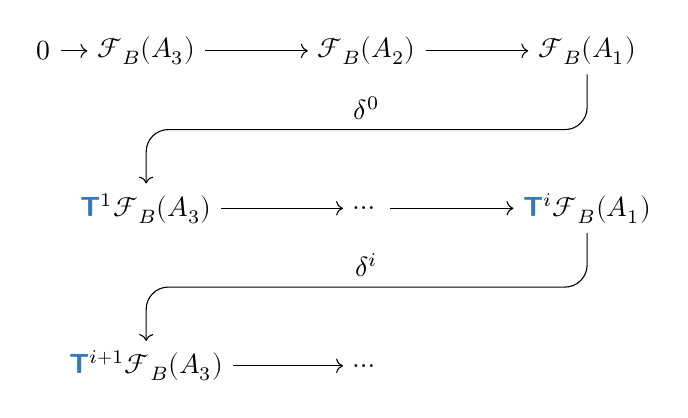
\begin{tikzpicture}[baseline=(current bounding box.center)]
        \node (zero) at (-1.3,2)
        {$0$}; \node (FA3) at (0,2)
        {$\mathscr{F}_B(A_3)$}; \node (FA2) at (2.8,2)
        {$\mathscr{F}_B(A_2)$}; \node (FA1) at (5.6,2)
        {$\mathscr{F}_B(A_1)$}; \node (T1A3) at (0,0)
        {$\categ{T}^1\mathscr{F}_B(A_3)$}; \node (dots1) at (2.8,0)
        {$\dots$}; \node (TiA1) at (5.6,0)
        {$\categ{T}^i\mathscr{F}_B(A_1)$}; \node (Ti1A3) at (0,-2)
        {$\categ{T}^{i+1}\mathscr{F}_B(A_3)$}; \node (dots2) at
        (2.8,-2)
        {$\dots$}; \draw[->] (zero) -- (FA3); \draw[->] (FA3) --
        (FA2); \draw[->] (FA2) -- (FA1); \draw[->] (T1A3) -- (dots1);
        \draw[->] (dots1) -- (TiA1); \draw[->] (Ti1A3) -- (dots2);
        \draw[->, rounded corners=8pt] (FA1.south) -- (5.6,1) --
        node[above]
        {$\delta^0$} (0,1) -- (T1A3.north); \draw[->, rounded
        corners=8pt] (TiA1.south) -- (5.6,-1) -- node[above]
        {$\delta^i$} (0,-1) -- (Ti1A3.north);
      \end{tikzpicture}
    \]
  \item Prove that the $\categ{T}^i\mathscr{F}_B$ form a
    $\delta$-functor, in the sense of Exercise~\ref{exer:homol:7.13}.
  \item Prove that if $E$ is an $\mathscr{F}$-exact object of
    $\categ{A}$, then $\categ{T}^i\mathscr{F}_B(E) = 0$ for $i > 0$,
    and deduce that the $\categ{T}^i\mathscr{F}_B$ form a
    \emph{universal} $\delta$-functor.
  \item Let
    $E^\bullet : \dots \to E^{-2} \to E^{-1} \to E^0 \to A \to 0$ be
    an $\mathscr{F}$-exact resolution of $A$. Then
    $\categ{T}^i\mathscr{F}_B \cong H^i(\mathscr{F}_B(E^\bullet))$.
    (Hint: Mimic the proof of Theorem~\ref{thm:homol:8.3}.)
  \end{itemize}
  The upshot is that the interplay of the two functors $\mathscr{F}^A$
  and $\mathscr{F}_B$ allows us to define $\categ{T}^i\mathscr{F}_B$
  as if it were a right-derived functor, using $\mathscr{F}$-exact
  objects in place of projectives. This gives a universal
  $\delta$-functor, which agrees with the standard right-derived
  functor when $\categ{A}$ has enough projectives (by
  Exercise~\ref{exer:homol:7.15} and the uniqueness of universal
  $\delta$-functors). [\S{}\ref{subsec:homol:resolution-by-acyclic-objects}]
\end{exer}

\section{Further topics}
\label{sec:homol:further-topics}

This last section touches upon issues that arise naturally in the
context of this chapter and for which a (much) more extensive
treatment would be needed. This will hopefully whet the reader's
appetite for more and encourage further study of homological algebra
beyond the basics covered here. I will be somewhat detailed in
\S{}9.3, illustrating the spectral sequence associated to a double
complex, since this can be done reasonably quickly (but delving into
any other application of spectral sequences would simply take us too
far). For the other themes in this section (derived and triangulated
categories) I will really do no more than a little propaganda.

\subsection{Derived categories}
\label{subsec:homol:derived-categories}
Derived categories made their appearance in \S{}4.2 and have since
served as a guiding concept motivating the natural development of the
subject, but we have stopped short of constructing them in
general. The closest we have come to a concrete description of the
derived category is in the `poor man's version' of \S{}6.3, which
should actually be labeled the `rich man's version', since it relies
on the fortunate presence of enough projectives/injectives. Also, the
versions $\categ{D}^-(\categ{A})$, $\categ{D}^+(\categ{A})$ considered
there are necessarily \emph{bounded}, as they rely on bounded
resolutions of objects and complexes in $\categ{A}$.  Derived
categories may be defined without such restrictions. For an abelian
category $\categ{A}$, the objects of $\categ{D}(\categ{A})$ are taken
to be the same as in $\categ{C}(\categ{A})$, that is, cochain
complexes; boundedness conditions may be included here, if desired. As
for morphisms, remember that the whole point of the derived category
is to `invert quasi-isomorphisms'; the most direct way to do this is
essentially the same as the process that allows us to `invert all
nonzero elements of an integral domain', leading to the construction
of the field of fractions (see \ref{subsec:irred:the-field-of-fractions-of-an-integral-domain}). This process, in a more
general version dealing with inverting `multiplicative subsets' of a
ring, is called \emph{localization} (\Cref{exer:irred:4.7}). Categories may
be localized as well. For example, the homotopic category
$\categ{K}(\categ{A})$ may be viewed as the localization of
$\categ{C}(\categ{A})$ with respect to homotopy equivalences: these
become isomorphisms in $\categ{K}(\categ{A})$.  Localizing
$\categ{K}(\categ{A})$ with respect to homotopy classes of
quasi-isomorphisms yields $\categ{D}(\categ{A})$.  In necessarily
oversimplified terms, suppose you want to make a class of morphisms of
a category $\categ{C}$ invertible. In the new category, any `roof'
diagram
\[\begin{tikzcd}
    & Z \arrow[dl,"\alpha"'] \arrow[dr,"\beta"] & \\
    A \arrow[rr,dashed] & & B
  \end{tikzcd}\] with $\alpha$ in that class will determine a morphism
$\beta \circ \alpha^{-1} : A \to B$; that is, the dashed arrow will
have to exist as a morphism in the new category. These are the analogs
of the `fractions' in the field of fractions; the localization of
$\categ{C}$ may be defined by taking the same objects as in
$\categ{C}$ and setting morphisms in the new category to be
compositions of `roofs', up to a suitable equivalence relation. For
example, all roofs
\[\begin{tikzcd}
    & Z \arrow[dl,"\alpha"'] \arrow[dr,"\alpha"] & \\
    A & & A
  \end{tikzcd}\] with $\alpha$ in the chosen class should be
identified to one another and to $\id_A$ in the
localized category; the roof
\[\begin{tikzcd}
    & Z \arrow[dl,"\alpha"'] \arrow[dr,"\id_Z"] & \\
    A & & Z
  \end{tikzcd}\] will work as the inverse of $\alpha$ in the
localization.

As the reader can imagine, working out the construction in earnest
requires dealing with nontrivial technical issues. These are more
manageable when the class of morphisms to be inverted is `localizing'
(for example, the composition of two such morphisms should also be a
morphism in the class); for example, this condition allows us to
represent the composition of two roofs as a roof. To mention one
set-theoretic difficulty, one should make sure that morphisms
$A \to B$ in the localization still form a \emph{set}, even if the
roofs connecting $A$ to $B$ may a priori form a proper \emph{class}.
With all these caveats in mind, the localization process can be
carried out on $\categ{K}(\categ{A})$ with respect to
quasi-isomorphisms and does produce a category $\categ{D}(\categ{A})$
satisfying the universal property for derived categories described in
\S{}4.2. If $\categ{A}$ has (for example) enough projectives, then the
bounded version $\categ{D}^-(\categ{A})$ is equivalent to the homotopy
category $\categ{K}^-(\categ{P})$ of complexes of projectives, as I
have endeavored to justify in \S{}6.3. The latter should be viewed as
a convenient way to `compute' the former in favorable circumstances.
Summarizing, a morphism $L^\bullet \to M^\bullet$ in the derived
category $\categ{D}(\categ{A})$ of an abelian category $\categ{A}$ can
be represented as a roof diagram
\[\begin{tikzcd}
    & N^\bullet \arrow[dl,"\text{quasi-isomorphism}"'] \arrow[dr] & \\
    L^\bullet & & M^\bullet
  \end{tikzcd}\] of (homotopy classes of) morphisms of cochain
complexes, modulo a suitable equivalence relation. Note that the
construction is applied to $\categ{K}(\categ{A})$, rather than the
simpler-minded $\categ{C}(\categ{A})$: for one thing, one might as
well start from $\categ{K}(\categ{A})$, since the functor
$\categ{C}(\categ{A}) \to \categ{D}(\categ{A})$ will have to factor
through the homotopic category (Proposition~\ref{prop:homol:5.4}). In
any case it just so happens that, unfortunately, quasi-isomorphisms do
not form a localizing class of morphisms in $\categ{C}(\categ{A})$,
while their homotopy classes \emph{are} localizing in
$\categ{K}(\categ{A})$. So it goes.  Once we believe that this
prescription does define a category---for example, that the
composition of two roofs can be represented by a roof and that this
composition is associative---then it is essentially clear that
$\categ{D}(\categ{A})$ satisfies the universal property specified in
\S{}4.2. However, the real benefits of introducing the derived
category lie deeper, for example in its structure as a
\emph{triangulated category}. A brief discussion of this concept
follows.

The reader should check that the composition of two roofs is indeed a
roof (Exercise~\ref{exer:homol:9.2}); this may be easier after
acquiring a little familiarity with distinguished triangles. Also,
note that the diagram in Exercise~\ref{exer:homol:9.2} does not
commute in $\categ{C}(\categ{A})$, but it does in
$\categ{K}(\categ{A})$. This is an indication that it would be
problematic to go `directly' from $\categ{C}(\categ{A})$ to
$\categ{D}(\categ{A})$.

\subsection{Triangulated categories}
\label{subsec:homol:triangulated-categories}
One reason for not treating derived categories to any real extent in
this book is that to do so would require us to define precisely the
notion of \emph{triangulated category}. The same applies in fact to
homotopic categories of complexes. I have pointed out in \S{}5.2 that
these categories should not be expected to be (and indeed are not)
\emph{abelian}, but they preserve enough structure to make sense of,
for example, long exact cohomology sequences. The fact that derived
functors ended up having long exact sequences associated to them
(\S{}7.4) bears witness to this fact.  The essential ingredients of a
triangulated (additive) category are a `translation' functor, which in
the case of $\categ{K}(\categ{A})$ or $\categ{D}(\categ{A})$ is
realized as the shift functor $L^\bullet \mapsto L[1]^\bullet$; and a
class of diagrams
\[
  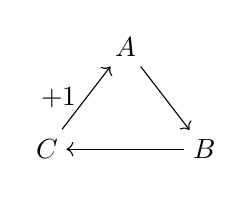
\begin{tikzpicture}[baseline=(current bounding box.center)]
    \node (A) at (1,1.3) {$A$}; \node (C) at (0,0)
    {$C$}; \node (B) at (2,0)
    {$B$}; \draw[->] (A) -- (B); \draw[->] (B) -- (C); \draw[->] (C)
    -- (A) node[midway, left] {$+1$};
  \end{tikzpicture}
\]
where the morphism labeled `$+1$' acts as $C \to A[1]$; these diagrams
are called \emph{distinguished triangles}. A common alternative
notation is
\[
  A \longrightarrow B \longrightarrow C \xrightarrow{+1}.
\]

Distinguished triangles are required to satisfy several axioms.  Among
them,
\[
  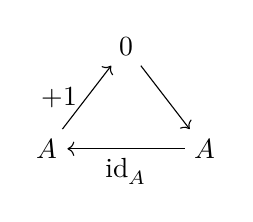
\begin{tikzpicture}[baseline=(current bounding box.center)]
    \node (T) at (1,1.3) {$0$}; \node (C) at (0,0)
    {$A$}; \node (B) at (2,0)
    {$A$}; \draw[->] (T) -- (B); \draw[->] (B) -- (C) node[midway,
    below]
    {$\id_A$}; \draw[->] (C) -- (T) node[midway, left]
    {$+1$};
  \end{tikzpicture}
\]
is required to be distinguished for every $A$; every morphism
$\alpha : A \to B$ must be a side of a distinguished triangle;
triangles isomorphic to a distinguished triangle (in the evident
sense) must be distinguished; and distinguished triangles can be
`rotated':
\[
  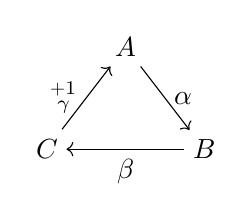
\begin{tikzpicture}[baseline=(current bounding box.center)]
    \node (A) at (1,1.3) {$A$}; \node (C) at (0,0)
    {$C$}; \node (B) at (2,0)
    {$B$}; \draw[->] (A) -- (B) node[midway, right]
    {$\alpha$}; \draw[->] (B) -- (C) node[midway, below]
    {$\beta$}; \draw[->] (C) -- (A) node[midway, left]
    {$\substack{+1\\\gamma}$};
  \end{tikzpicture}
\]
is distinguished if and only if
\[
  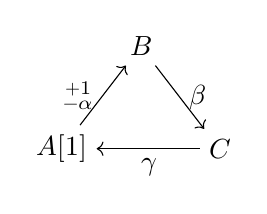
\begin{tikzpicture}[baseline=(current bounding box.center)]
    \node (B) at (1,1.3) {$B$}; \node (A) at (0,0)
    {$A[1]$}; \node (C) at (2,0)
    {$C$}; \draw[->] (B) -- (C) node[midway, right]
    {$\beta$}; \draw[->] (C) -- (A) node[midway, below]
    {$\gamma$}; \draw[->] (A) -- (B) node[midway, left]
    {$\substack{+1\\-\alpha}$};
  \end{tikzpicture}
\]
is distinguished. There is more, including an infamous
\emph{octahedral axiom} (so named since a popular way to state it
invokes an octahedral diagram). The reader will have no difficulties
locating this information in the literature.  The category
$\categ{K}(\categ{A})$ is triangulated: the translation functor is the
basic shift of a complex, and distinguished triangles are those
isomorphic to
\[
  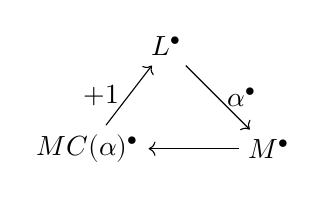
\begin{tikzpicture}[baseline=(current bounding box.center)]
    \node (L) at (1,1.3)
    {$L^\bullet$}; \node (MC) at (0,0)
    {$MC(\alpha)^\bullet$}; \node (M) at (2.3,0)
    {$M^\bullet$}; \draw[->] (L) -- (M) node[midway, right]
    {$\alpha^\bullet$}; \draw[->] (M) -- (MC); \draw[->] (MC) -- (L)
    node[midway, left] {$+1$};
  \end{tikzpicture}
\]
That is, the `third vertex' of a triangle with an assigned side
$\alpha^\bullet : L^\bullet \to M^\bullet$ is the mapping cone of
$\alpha^\bullet$, and the unlabeled sides are the natural cochain
morphisms $M^\bullet \to MC(\alpha)^\bullet$,
$MC(\alpha)^\bullet \to L[1]^\bullet$ studied in \S{}4.1.

It would be problematic to make the same choice in
$\categ{C}(\categ{A})$, since while
\[
  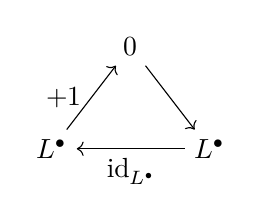
\begin{tikzpicture}[baseline=(current bounding box.center)]
    \node (T) at (1,1.3) {$0$}; \node (Z) at (0,0)
    {$L^\bullet$}; \node (B) at (2,0)
    {$L^\bullet$}; \draw[->] (T) -- (B); \draw[->] (B) -- (Z)
    node[midway, below]
    {$\id_{L^\bullet}$}; \draw[->] (Z) -- (T)
    node[midway, left] {$+1$};
  \end{tikzpicture}
\]
would be distinguished as needed, since $L^\bullet$ is the mapping
cone of the zero-morphism $0 \to L^\bullet$, the rotation of this
triangle, i.e.,
\[
  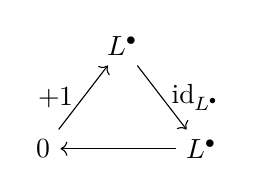
\begin{tikzpicture}[baseline=(current bounding box.center)]
    \node (L) at (1,1.3) {$L^\bullet$}; \node (Z) at (0,0)
    {$0$}; \node (B) at (2,0)
    {$L^\bullet$}; \draw[->] (L) -- (B) node[midway, right]
    {$\id_{L^\bullet}$}; \draw[->] (B) -- (Z); \draw[->]
    (Z) -- (L) node[midway, left] {$+1$};
  \end{tikzpicture}
\]
would not seem to be, since the mapping cone of the identity is not
$0$. But the mapping cone of the identity is \emph{homotopically
  equivalent} to $0$ (Exercise~\ref{exer:homol:9.3}), so the rotated
triangle is indeed distinguished in $\categ{K}(\categ{A})$, as it
should be, according to the axioms. More generally, it is easy to see
(Exercise~\ref{exer:homol:9.4}) that if
$\alpha^\bullet : L^\bullet \to M^\bullet$ is a cochain morphism, so
that we have a distinguished triangle,
\[
  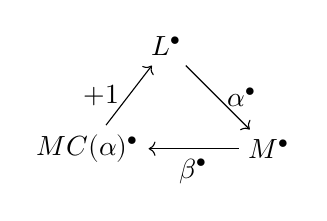
\begin{tikzpicture}[baseline=(current bounding box.center)]
    \node (L) at (1,1.3)
    {$L^\bullet$}; \node (MC) at (0,0)
    {$MC(\alpha)^\bullet$}; \node (M) at (2.3,0)
    {$M^\bullet$}; \draw[->] (L) -- (M) node[midway, right]
    {$\alpha^\bullet$}; \draw[->] (M) -- (MC) node[midway, below]
    {$\beta^\bullet$}; \draw[->] (MC) -- (L) node[midway, left]
    {$+1$};
  \end{tikzpicture}
\]
then the mapping cone of $\beta^\bullet$ is in fact homotopy
equivalent to $L[1]^\bullet$; the rotation
\[
  (*) \qquad
  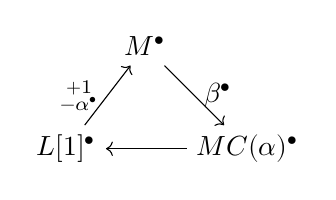
\begin{tikzpicture}[baseline=(current bounding box.center)]
    \node (M) at (1,1.3)
    {$M^\bullet$}; \node (L1) at (0,0)
    {$L[1]^\bullet$}; \node (MC) at (2.3,0)
    {$MC(\alpha)^\bullet$}; \draw[->] (M) -- (MC) node[midway, right]
    {$\beta^\bullet$}; \draw[->] (MC) -- (L1); \draw[->] (L1) -- (M)
    node[midway, left] {$\substack{+1\\-\alpha^\bullet}$};
  \end{tikzpicture}
\]
is distinguished as required, as the reader should check.
\emph{Applying the cohomology functor to a distinguished triangle in
  $\categ{K}(\categ{A})$ yields an exact triangle}: indeed, as we have
just seen, we may assume that the triangle is $(*)$ (up to isomorphism
in $\categ{K}(\categ{A})$), and taking cohomology gives the exact
triangle
\[
  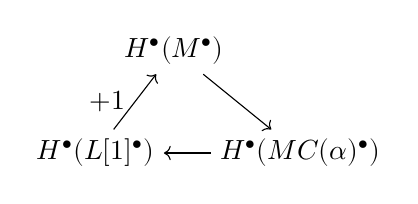
\begin{tikzpicture}[baseline=(current bounding box.center)]
    \node (M) at (1,1.3)
    {$H^\bullet(M^\bullet)$}; \node (L1) at (0,0)
    {$H^\bullet(L[1]^\bullet)$}; \node (MC) at (2.6,0)
    {$H^\bullet(MC(\alpha)^\bullet)$}; \draw[->] (M) -- (MC);
    \draw[->] (MC) -- (L1); \draw[->] (L1) -- (M) node[midway, left]
    {$+1$};
  \end{tikzpicture}
\]
obtained in Proposition~\ref{homol:4.1}. In general, a
\emph{cohomological functor} on a triangulated category is an additive
functor to an abelian category, mapping distinguished triangles to
exact triangles and hence inducing long exact sequences. Thus,
cohomology is a cohomological functor on $\categ{K}(\categ{A})$; this
will not surprise the reader. The functors $\Hom(A,\_)$
and $\Hom(\_,A)$ (to $\categ{Ab}$) are cohomological
functors on every triangulated category, for every object $A$.

The derived category $\categ{D}(\categ{A})$ and its bounded versions
are triangulated categories, with distinguished triangles described as
above---that is, isomorphic (in $\categ{D}(\categ{A})$) to the basic
triangles determined by mapping cones. The natural functor
$\categ{K}(\categ{A}) \to \categ{D}(\categ{A})$ is a functor of
triangulated categories, in the sense that it preserves the
translation functor and it sends distinguished triangles to
distinguished triangles.

Isomorphism in the derived category is a less stringent notion than in
the homotopic category, so there are `more' distinguished triangles in
$\categ{D}(\categ{A})$ than in $\categ{K}(\categ{A})$.  For example,
if
\[
  0 \longrightarrow L^\bullet \xrightarrow{\alpha^\bullet} M^\bullet
  \xrightarrow{\beta^\bullet} N^\bullet \longrightarrow 0
\]
is a short exact sequence, as above, there is in general no
distinguished triangle
\[
  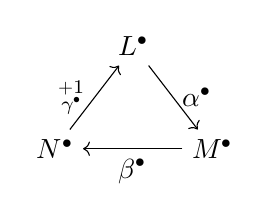
\begin{tikzpicture}[baseline=(current bounding box.center)]
    \node (L) at (1,1.3)
    {$L^\bullet$}; \node (N) at (0,0)
    {$N^\bullet$}; \node (M) at (2,0)
    {$M^\bullet$}; \draw[->] (L) -- (M) node[midway, right]
    {$\alpha^\bullet$}; \draw[->] (M) -- (N) node[midway, below]
    {$\beta^\bullet$}; \draw[->] (N) -- (L) node[midway, left]
    {$\substack{+1\\\gamma^\bullet}$};
  \end{tikzpicture}
\]
in $\categ{K}(\categ{A})$ (for any choice of $\gamma^\bullet$):
indeed, $N^\bullet$ need not\footnote{Why? Construct an example
  showing this.} be homotopically equivalent to $MC(\alpha)^\bullet$.
But such triangles \emph{do} exist in $\categ{D}(\categ{A})$!  In
fact, we are now well-equipped to make (better) sense of the
mysterious remarks at the end of \S{}3.4. The `special triangles'
\[
  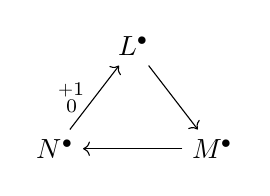
\begin{tikzpicture}[baseline=(current bounding box.center)]
    \node (L) at (1,1.3)
    {$L^\bullet$}; \node (N) at (0,0)
    {$N^\bullet$}; \node (M) at (2,0)
    {$M^\bullet$}; \draw[->] (L) -- (M); \draw[->] (M) -- (N);
    \draw[->] (N) -- (L) node[midway, left] {$\substack{+1\\0}$};
  \end{tikzpicture}
\]
arising as in \S{}3.4 from a short exact sequence
\[
  0 \longrightarrow L^\bullet \xrightarrow{\alpha^\bullet} M^\bullet
  \xrightarrow{\beta^\bullet} N^\bullet \longrightarrow 0
\]
are not distinguished in $\categ{K}(\categ{A})$, and in general no
replacement for the zero-morphism will fix this problem. On the other
hand, the reader can now verify (Exercise~\ref{exer:homol:9.5}) that
there is a quasi-isomorphism $MC(\alpha)^\bullet \to N^\bullet$: this
can be shown by computing explicitly another mapping cone and applying
Corollary~\ref{homol:4.2}. Thus, in the derived category the standard
distinguished triangle
\[
  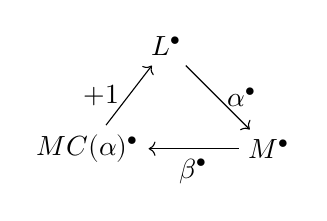
\begin{tikzpicture}[baseline=(current bounding box.center)]
    \node (L) at (1,1.3)
    {$L^\bullet$}; \node (MC) at (0,0)
    {$MC(\alpha)^\bullet$}; \node (M) at (2.3,0)
    {$M^\bullet$}; \draw[->] (L) -- (M) node[midway, right]
    {$\alpha^\bullet$}; \draw[->] (M) -- (MC) node[midway, below]
    {$\beta^\bullet$}; \draw[->] (MC) -- (L) node[midway, left]
    {$+1$};
  \end{tikzpicture}
\]
is isomorphic to a triangle
\[
  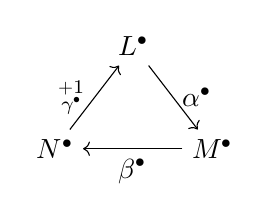
\begin{tikzpicture}[baseline=(current bounding box.center)]
    \node (L) at (1,1.3)
    {$L^\bullet$}; \node (N) at (0,0)
    {$N^\bullet$}; \node (M) at (2,0)
    {$M^\bullet$}; \draw[->] (L) -- (M) node[midway, right]
    {$\alpha^\bullet$}; \draw[->] (M) -- (N) node[midway, below]
    {$\beta^\bullet$}; \draw[->] (N) -- (L) node[midway, left]
    {$\substack{+1\\\gamma^\bullet}$};
  \end{tikzpicture}
\]
which is therefore distinguished in $\categ{D}(\categ{A})$ (cf.\
Exercise~\ref{exer:homol:9.6}). Applying the cohomology functor to
this triangle directly gives the exact triangle
\[
  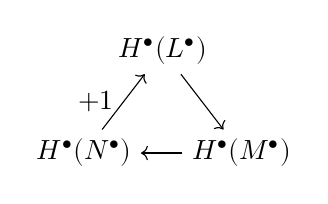
\begin{tikzpicture}[baseline=(current bounding box.center)]
    \node (L) at (1,1.3)
    {$H^\bullet(L^\bullet)$}; \node (N) at (0,0)
    {$H^\bullet(N^\bullet)$}; \node (M) at (2,0)
    {$H^\bullet(M^\bullet)$}; \draw[->] (L) -- (M); \draw[->] (M) --
    (N); \draw[->] (N) -- (L) node[midway, left] {$+1$};
  \end{tikzpicture}
\]
expressing the long exact cohomology sequence as in \S{}3.4, without
having to single out the $+1$ morphism for special consideration. In
retrospect, the zero-morphism I insisted on using when folding
`special' triangles in \S{}3.4 turns out to be an artifact: placing
the triangle in the derived category shows that there is a more
informed choice for this morphism. This choice is not available in
$\categ{C}(\categ{A})$ and is not even in $\categ{K}(\categ{A})$, but
it \emph{is} available in $\categ{D}(\categ{A})$ and leads
transparently to the long exact sequence in cohomology.

If $\mathscr{F} : \categ{A} \to \categ{B}$ is a functor between
abelian categories, the induced functor
$\categ{K}(\mathscr{F}) : \categ{K}(\categ{A}) \to
\categ{K}(\categ{B})$ is a functor of triangulated categories, and so
are the bounded variations
$\categ{K}^\pm(\mathscr{F}) : \categ{K}^\pm(\categ{A}) \to
\categ{K}^\pm(\categ{B})$. The derived functors
$\categ{L}\mathscr{F}, \categ{R}\mathscr{F} : \categ{D}^\pm(\categ{A})
\to \categ{D}^\pm(\categ{B})$ encountered in \S{}7.2 are also functors
of triangulated categories.  This fact is responsible for the good
properties of derived functors, such as the long exact sequences
studied in \S{}7.4.

\subsection{Spectral sequences}
\label{subsec:homol:spectral-sequences}
I mentioned in \S{}8.3 that `spectral sequences' may be used to
compute the cohomology of a double complex. There unfortunately does
not seem to be an easy entry point in the subject of spectral
sequences, which is marred by intrinsic notational complexity. I will
limit myself to a very scant description of the concept and some
information linking it back to \S{}8.4. My motivation is that, in the
literature, references to results such as \Cref{thm:homol:8.12} are often
replaced by sentences such as `by an immediate spectral sequence
argument\dots', and I should try to explain to the reader what this
means.

Given that we were thinking about triangles a moment ago, the
following construction may be helpful in appreciating the notion of
spectral sequence. Let
\[
  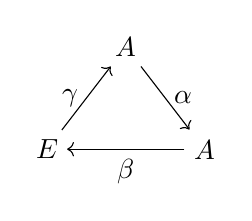
\begin{tikzpicture}[baseline=(current bounding box.center)]
    \node (A) at (1,1.3) {$A$}; \node (E) at (0,0)
    {$E$}; \node (A2) at (2,0)
    {$A$}; \draw[->] (A) -- (A2) node[midway, right]
    {$\alpha$}; \draw[->] (A2) -- (E) node[midway, below]
    {$\beta$}; \draw[->] (E) -- (A) node[midway, left] {$\gamma$};
  \end{tikzpicture}
\]
be an exact triangle\footnote{That is,
  $\image\alpha = \ker\beta$,
  $\image\beta = \ker\gamma$, and
  $\image\gamma = \ker\alpha$.} in an abelian category; I
am placing no assumption on the `degree' of $\gamma$ (and indeed, I am
not assuming we have defined a translation functor).

Let $d : E \to E$ be the composition $\beta \circ \gamma$; since
$\gamma \circ \beta = 0$, we have
\[
  d \circ d = \beta \circ (\gamma \circ \beta) \circ \gamma = 0.
\]
Thus we can take the homology of $E$ with respect to $d$ and define
\[
  E' := \frac{\ker d}{\image d}.
\]
Further, we can let $A' := \image\alpha$ and let
\begin{itemize}
\item $\alpha' : A' \to A'$ be the restriction of $\alpha$ to $A'$;
\item $\beta' : A' \to E'$ be defined by
  $\beta'(\alpha(a)) := [\beta(a)]$;
\item $\gamma' : E' \to A'$ be defined by $\gamma'([e]) := \gamma(e)$,
\end{itemize}
where $[e]$ denotes the class of $e \in E$ in $E'$. (Since
$\beta \circ \gamma(e) = d(e) = 0$,
$\gamma(e) \in \ker\beta = \image\alpha = A'$.) All needed
verifications (such as the independence on the representative $e$ of
$[e]$ in the third prescription) are straightforward, from the
exactness of the given triangle.

\begin{fact}{\Cref{fact:homol:9.1}}{fact:homol:9.1}
  The new triangle
  \[
    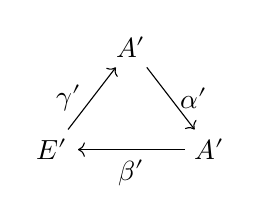
\begin{tikzpicture}[baseline=(current bounding box.center)]
      \node (A) at (1,1.3) {$A'$}; \node (E) at (0,0)
      {$E'$}; \node (A2) at (2,0)
      {$A'$}; \draw[->] (A) -- (A2) node[midway, right]
      {$\alpha'$}; \draw[->] (A2) -- (E) node[midway, below]
      {$\beta'$}; \draw[->] (E) -- (A) node[midway, left] {$\gamma'$};
    \end{tikzpicture}
  \]
  is again exact.
\end{fact}

The reader will have no difficulty proving this statement
(Exercise~\ref{exer:homol:9.7}).

The datum of an exact triangle as above is called an \emph{exact
  couple}, which I find confusing since a triangle has three vertices
(but it is true that only two objects are involved here); the new
exact triangle (couple) obtained in Claim~\ref{fact:homol:9.1} is the
\emph{derived couple}, which I find even more confusing since there is
no derived category or functor in sight. Exact couples arose in
topology (they are due to W. Massey), and the terminology reflects
their origin.

Of course we can turn the crank at will and get derived couple after
derived couple: let $A_1 = A$, $E_1 = E$, etc., and inductively define
$A_{i+1} := A'_i$, $E_{i+1} := E'_i$, etc. For example, $\beta_{i+1}$
is obtained by `rewinding' the morphism $\alpha$ a total of $i$ times
and then applying the original morphism $\beta$: we can do this since
$A_{i+1}$ is the image of $\alpha^i$.

Thus, one exact triangle produces a whole sequence of triangles and in
particular a sequence of objects $E_i$, each endowed with a
differential $d_i$, such that
$E_{i+1} = \ker d_i / \image d_i$.

\begin{defn}{}{defn:homol:9.2}
  A \emph{spectral sequence} $\{(E_i, d_i)\}_{i=1,2,\dots}$ is a
  sequence of objects $E_i$ and morphisms $d_i : E_i \to E_i$ in an
  abelian category, such that $d_i \circ d_i = 0$ and
  $E_{i+1} \cong \ker d_i / \image d_i$.
\end{defn}

Thus, exact couples are a way to produce spectral sequences. There is
a sense in which we can turn the crank `infinitely many times'; in
fact, this can be done with any spectral sequence. To see this, let
\[
  Z_1 = E_1, \quad B_1 = 0,
\]
so that $E_1 \cong Z_1/B_1$; inductively, assume we have defined
$Z_i \subseteq Z_1$, $B_i \subseteq Z_i$ so that $E_i \cong Z_i/B_i$,
and let $\overline{Z}_{i+1} = \ker d_i$,
$\overline{B}_{i+1} = \image d_i$; define $Z_{i+1}$,
$B_{i+1}$ as the corresponding subobjects of $Z_i$. Then
\[
  E_{i+1} \cong \frac{\overline{Z}_{i+1}}{\overline{B}_{i+1}} \cong
  \frac{Z_{i+1}}{B_{i+1}},
\]
realizing $E_{i+1}$ as a \emph{subquotient}\footnote{That is, as a
  quotient of a subobject.} of $E_1$, and
\[
  B_1 \subseteq \dots \subseteq B_i \subseteq B_{i+1} \subseteq \dots
  \subseteq Z_{i+1} \subseteq Z_i \subseteq \dots \subseteq Z_1.
\]
Define\footnote{Here I am implicitly working in a category
  $R\text{-}\categ{Mod}$ of modules over a ring, containing the given
  abelian category $\categ{A}$ (invoking the Freyd--Mitchell theorem,
  Theorem~\ref{homol:2.9}). The infinite unions and intersections used
  here make sense in $R\text{-}\categ{Mod}$; the limits and the
  corresponding $E_\infty$ are therefore defined as objects in
  $R\text{-}\categ{Mod}$ and in general not as objects of $\categ{A}$.
  But if, e.g., the sequence collapses at $E_r$, then
  $B_\infty = B_r$, $Z_\infty = Z_r$, and $E_\infty$ exists in
  $\categ{A}$. In practice, this difficulty will play no role in the
  considerations that follow.}
\[
  B_\infty := \bigcup_i B_i, \quad Z_\infty := \bigcap_i Z_i, \quad
  E_\infty := \frac{Z_\infty}{B_\infty}.
\]
This `ultimate' subquotient $E_\infty$ is the \emph{limit} of the
spectral sequence; it is common to say that the spectral sequence
$E_r$ \emph{abuts} to $E_\infty$. By definition, if
$d_r = d_{r+1} = \dots = 0$, then $Z_\infty = Z_r$ and
$B_\infty = B_r$, so that $E_\infty \cong E_r$; in this case we say
that the sequence \emph{collapses} at $E_r$.

The reader will verify (Exercise~\ref{exer:homol:9.8}) that if the
spectral sequence arises from an exact couple, as above, then
\[
  Z_\infty = \bigcap_r \gamma^{-1}(\image \alpha^r), \quad
  B_\infty = \bigcup_r \beta(\ker \alpha^r),
\]
so the limit $E_\infty$ has a concrete realization in this case.

Typically, a spectral sequence is as interesting as its limit,
especially if some fortunate circumstance causes its collapse very
soon; it is not too uncommon to have situations in which
$E_\infty = E_2$. If all goes well, this translates into a useful
relation between the given `input' $E_1$ and the interesting `output'
$E_\infty$.  \emph{Where is my double complex?} I promised that
spectral sequences could be used to `compute' the cohomology of the
total complex of a double complex. We will now see how a double
complex gives rise to an exact couple and hence to a spectral
sequence. This is a particular case of a useful mechanism producing an
exact sequence from a filtration.

A `descending filtration' of $M$ consists of a sequence of subobjects:
\[
  M \supseteq \dots \supseteq M_m \supseteq M_{m+1} \supseteq \dots.
\]
For example, the series of subgroups of a group $G$ considered in
\ref{subsec:groups2:the-jordan-h-older-theorem} are filtrations of $G$. If $M$ is an object of an abelian
category, a filtration as above determines an associated \emph{graded
  object}
\[
  \operatorname{gr}(M) := \bigoplus_m \operatorname{gr}(M)_m, \quad
  \operatorname{gr}(M)_m := \frac{M_m}{M_{m+1}};
\]
I will assume this is an object of the same category for simplicity,
although this is not necessarily the case (abelian categories are not
necessarily closed under infinite direct sums); since only finitely
many objects will be involved in any specific computation, this plays
no role.

Start with a double complex $M^{\bullet,\bullet}$; I will assume that
$M^{i,j} = 0$ for $i < 0$, $j < 0$:
\[\begin{tikzcd}
    \vdots & \vdots & \vdots & \vdots & \\
    M^{0,2} \arrow[r,"d_h"] \arrow[u,"\delta_v"] & M^{1,2} \arrow[r,"d_h"] \arrow[u,"\delta_v"] & M^{2,2} \arrow[r,"d_h"] \arrow[u,"\delta_v"] & M^{3,2} \arrow[r,"d_h"] \arrow[u,"\delta_v"] & \cdots \\
    M^{0,1} \arrow[r,"d_h"] \arrow[u,"\delta_v"] & M^{1,1} \arrow[r,"d_h"] \arrow[u,"\delta_v"] & M^{2,1} \arrow[r,"d_h"] \arrow[u,"\delta_v"] & M^{3,1} \arrow[r,"d_h"] \arrow[u,"\delta_v"] & \cdots \\
    M^{0,0} \arrow[r,"d_h"] \arrow[u,"\delta_v"] & M^{1,0}
    \arrow[r,"d_h"] \arrow[u,"\delta_v"] & M^{2,0} \arrow[r,"d_h"]
    \arrow[u,"\delta_v"] & M^{3,0} \arrow[r,"d_h"]
    \arrow[u,"\delta_v"] & \cdots
  \end{tikzcd}\] As always, zero-objects to the left and below the
given part of the diagram are implicit; we are assuming (as in
\Cref{defn:homol:8.5}) that the diagram anticommutes, so that the
differential of the total complex $TC(M)^\bullet$ is simply
$d_h + \delta_v$. Analogous results can be obtained if $M^{i,j} = 0$
for $i > 0$, $j > 0$ and in fact under more relaxed hypotheses; such
considerations are left to the reader.

Let $T^\bullet = TC(M)^\bullet$ denote the total complex: therefore,
$T^k = \bigoplus_{i+j=k} M^{i,j}$. This complex admits (at least) two
filtrations: a \emph{horizontal} filtration and a \emph{vertical}
filtration. I will focus on the vertical one, and again it is
understood that a parallel discussion would hold for the horizontal
one. The vertical filtration $T^\bullet_m$ is defined by chopping off
the terms to the left of a vertical bar $i = m$ in the diagram
\[\begin{tikzcd}
    & \vdots & \vdots & \\
    \cdots & M^{m,2} \arrow[r,"d_h"] \arrow[u,"\delta_v"] & M^{m+1,2} \arrow[r,"d_h"] \arrow[u,"\delta_v"] & \cdots \\
    \cdots & M^{m,1} \arrow[r,"d_h"] \arrow[u,"\delta_v"] & M^{m+1,1} \arrow[r,"d_h"] \arrow[u,"\delta_v"] & \cdots \\
    \cdots & M^{m,0} \arrow[r,"d_h"] \arrow[u,"\delta_v"] & M^{m+1,0}
    \arrow[r,"d_h"] \arrow[u,"\delta_v"] & \cdots
  \end{tikzcd}\] That is, we set
\[
  T_m^k := \bigoplus_{\substack{i+j=k\\i \ge m}} M^{i,j},
\]
still with differential $d_h + \delta_v$. I will denote the
corresponding graded object by $\operatorname{gr}^\bullet_v(T)$, to
record the fact that this arises from the vertical filtration. (The
$\bullet$ reminds us that this is still a complex.) Explicitly, the
term of `filtration degree' $m$ in $\operatorname{gr}^k_v(T)$ is
\[
  \operatorname{gr}^k_v(T)_m = T_m^k / T_{m+1}^k = \bigoplus_{i \ge m}
  M^{i,k-i} \Big/ \bigoplus_{i \ge m+1} M^{i,k-i} \cong M^{m,k-m}.
\]
The differential $d_h + \delta_v$ induces the differential $\delta_v$
on this graded piece, since $d_h$ is zero modulo the next piece of the
filtration. The modules on the original array can therefore be labeled
as follows:
% ..  ..  ..  ..  . O K K K K K . O K K K K K . O K K K K K . O F F F
% F F
\[\begin{tikzcd}[column sep=small]
    \vdots & \vdots & \vdots & \vdots & \\
    \operatorname{gr}^2_v(T)_0 \arrow[r,dashed] & \operatorname{gr}^3_v(T)_1 \arrow[r,dashed] & \operatorname{gr}^4_v(T)_2 \arrow[r,dashed] & \operatorname{gr}^5_v(T)_3 & \cdots \\
    \operatorname{gr}^1_v(T)_0 \arrow[u] \arrow[r,dashed] & \operatorname{gr}^2_v(T)_1 \arrow[u] \arrow[r,dashed] & \operatorname{gr}^3_v(T)_2 \arrow[u] \arrow[r,dashed] & \operatorname{gr}^4_v(T)_3 \arrow[u] & \cdots \\
    \operatorname{gr}^0_v(T)_0 \arrow[u] \arrow[r,dashed] &
    \operatorname{gr}^1_v(T)_1 \arrow[u] \arrow[r,dashed] &
    \operatorname{gr}^2_v(T)_2 \arrow[u] \arrow[r,dashed] &
    \operatorname{gr}^3_v(T)_3 \arrow[u] & \cdots
  \end{tikzcd}\] with dashes connecting pieces with the same degree in
$\operatorname{gr}^\bullet_v(T)$.

The filtration on $T^\bullet$ also determines a filtration on the
cohomology of $T^\bullet$: we can take $H^\bullet(T^\bullet)_m$ to be
the image in $H^\bullet(T^\bullet)$ of $H^\bullet(T_m^\bullet)$.
Thus, we also have a graded object
$\operatorname{gr}_v H^\bullet(T^\bullet)$. \emph{The relation between
  $H^\bullet(\operatorname{gr}_v^\bullet(T))$ and
  $\operatorname{gr}_v H^\bullet(T^\bullet)$ is subtle: this relation
  is what spectral sequences will help us understand.}

The monomorphisms $T_{m+1}^\bullet \subseteq T_m^\bullet$ define a
monomorphism $\bigoplus_m T_m^\bullet \to \bigoplus_m T_m^\bullet$, of
which $\operatorname{gr}_v^\bullet(T)$ is the cokernel: we have an
exact sequence
\[
  (\dagger) \qquad 0 \longrightarrow \bigoplus_m T_m^\bullet
  \longrightarrow \bigoplus_m T_m^\bullet \longrightarrow
  \operatorname{gr}_v^\bullet(T) \longrightarrow 0 \, .
\]
As we know since \S{}3.3, this determines an exact triangle (couple!)
\[
  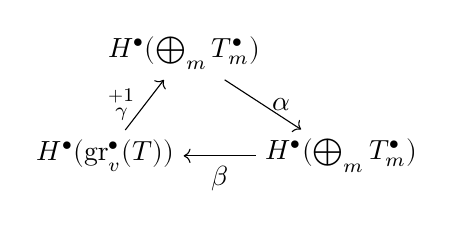
\begin{tikzpicture}[baseline=(current bounding box.center)]
    \node (A) at (1,1.3) {$H^\bullet(\bigoplus_m
      T_m^\bullet)$}; \node (E) at (0,0)
    {$H^\bullet(\operatorname{gr}_v^\bullet(T))$}; \node (A2) at (3,0)
    {$H^\bullet(\bigoplus_m
      T_m^\bullet)$}; \draw[->] (A) -- (A2) node[midway, right]
    {$\alpha$}; \draw[->] (A2) -- (E) node[midway, below]
    {$\beta$}; \draw[->] (E) -- (A) node[midway, left]
    {$\substack{+1\\\gamma}$};
  \end{tikzpicture}
\]
Note that $\alpha$ decreases the filtration degree by $1$, leaving the
cohomology degree $k$ unchanged; $\beta$ leaves both unchanged; and
$\gamma$ increases both by $1$. This is particularly clear if one
draws a small slice of the sequence $(\dagger)$, sufficient to see the
connecting morphism in action on a piece of given filtration and
cohomology degrees:
\[\begin{tikzcd}
    0 \arrow[r] & T_{m+1}^{k+1} \arrow[r] & T_m^{k+1} \arrow[r] &
    \operatorname{gr}_v^{k+1}(T)_m \arrow[r] & 0 \\
    0 \arrow[r] & T_{m+1}^k \arrow[r] \arrow[u] & T_m^k \arrow[r]
    \arrow[u] & \operatorname{gr}_v^k(T)_m \arrow[r] \arrow[u]
    \arrow[from=2-4,to=1-2,dashed,"\gamma" description, bend left=15]
    & 0
  \end{tikzcd}\]

\begin{defn}{}{defn:homol:9.3}
  The \emph{spectral sequence of the double complex}
  $M^{\bullet,\bullet}$ (with respect to the vertical filtration) is
  the spectral sequence determined by this exact couple.
\end{defn}

I will denote this spectral sequence by ${}_vE$, with the absurdly
positioned index $v$ recording that ${}_vE$ arises from the
\emph{vertical} filtration. The horizontal filtration leads likewise
to a spectral sequence ${}_hE$.

All terms ${}_vE_r$ of the spectral sequence are subquotients of the
first one, ${}_vE_1 = H^\bullet(\operatorname{gr}_v^\bullet(T))$.

\begin{rem}{}{homol:9.4}
  The differential $d_r = \beta_r \circ \gamma_r$ acts by increasing
  the cohomological degree $k$ by $1$ and the filtration degree $m$ by
  $r$: indeed, $\gamma_r$ is simply
  % induced by \gamma , so it increases both k and m by 1 (as observed
  % above); \beta r is obtained by applying \beta
  after undoing $(r-1)$ times the effect of $\alpha$ (as pointed out
  after Claim~\ref{fact:homol:9.1}), so it does not change $k$ but
  increases $m$ by $(r-1)$.
\end{rem}

Interest in the sequence rests on the interpretation for its limit in
the statement that follows, which also summarizes the situation.

\begin{thm}{}{homol:9.5}
  Let $M^{\bullet,\bullet}$ be a double complex in an abelian
  category. Assume that $M^{i,j} = 0$ for $i < 0$, $j < 0$, and let
  $T^\bullet$ be the total complex of $M^{\bullet,\bullet}$. Then,
  with notation as above, there exists a spectral sequence
  $\{({}_vE_i, d_i)\}_i$ such that
  \[ {}_vE_1 \cong H^\bullet(\operatorname{gr}_v^\bullet(T)), \qquad
    {}_vE_\infty \cong \operatorname{gr}_v H^\bullet(T^\bullet).
  \]
  In other words, `turning the crank' moves the $\operatorname{gr}$
  from inside the cohomology to outside of it. The limit
  ${}_vE_\infty$ does not quite compute the cohomology of the total
  complex, as I glibly announced in \S{}8.3, but it computes the
  graded object determined by a filtration on the cohomology of the
  total complex, and this is good enough for many applications.
\end{thm}
% Proof. The limit v E \infty can be computed directly from the exact
% couple (Exer- cise 9.8), as a subquotient of v E 1 : it is the
% quotient Z\infty /B\infty , where
\begin{proof}
  The limit ${}_vE_\infty$ can be computed directly from the exact
  couple (Exercise~\ref{exer:homol:9.8}), as a subquotient of
  ${}_vE_1$: it is the quotient $Z_\infty/B_\infty$, where
  \[
    Z_\infty = \bigcap_r \gamma^{-1}(\image\alpha^r),
    \qquad B_\infty = \beta\Big(\bigcup_r \ker\alpha^r\Big).
  \]
  The computation is streamlined by focusing on a specific degree $k$
  for the cohomology and $m$ for the grading. The corresponding part
  in ${}_vE_1$ is $H^k(T_m^\bullet/T_{m+1}^\bullet)$, and $\alpha$
  acts as $H^k(T_m^\bullet) \to H^k(T_{m-1}^\bullet)$. Note that if
  $r \gg 0$, then
  \[
    H^k(T_{m+r}^\bullet) = 0, \qquad H^k(T_{m-r}^\bullet) =
    H^k(T^\bullet),
  \]
  under our boundedness hypothesis: indeed, $T_i^j = 0$ if $i > j$,
  and $T_i^\bullet = T^\bullet$ for $i \le 0$.

  By the first of these observations, the piece sent by $\alpha^r$ to
  $H^k(T_m^\bullet)$ is $0$ for $r \gg 0$, and it follows that
  $\bigcap_r \image\alpha^r = 0$. Therefore,
  \[
    Z_\infty = \ker\gamma = \image\beta.
  \]
  By the second observation, $\ker\alpha^r$ stabilizes to
  $\ker(H^k(T_m^\bullet) \to H^k(T^\bullet))$ for each $k$, hence
  \[
    B_\infty = \beta\Big(\bigoplus_m \ker(H^\bullet(T_m^\bullet) \to
    H^\bullet(T^\bullet))\Big).
  \]

  Denote by $\nu_m : H^\bullet(T_m^\bullet) \to H^\bullet(T^\bullet)$
  the morphisms induced in cohomology by the monomorphisms
  $T_m^\bullet \to T^\bullet$ and by $\nu = \bigoplus_m \nu_m$ their
  direct sum. We have morphisms
  \[
    H^\bullet(\operatorname{gr}_v^\bullet(T)) \xleftarrow{\ \beta\ }
    \bigoplus_m H^\bullet(T_m^\bullet) \xrightarrow{\ \nu\ }
    \bigoplus_m H^\bullet(T^\bullet),
  \]
  and we have obtained
  \[ {}_vE_\infty \cong \frac{\image\beta}{\beta(\ker\nu)}.
  \]

  By the innocent \Cref{exer:homol:2.12},
  \[
    \frac{\image\beta}{\beta(\ker\nu)} \cong
    \frac{\image\nu}{\nu(\ker\beta)};
  \]
  by the exactness of the original couple,
  \[
    \ker\beta = \image\alpha = \bigoplus_m
    \image(H^\bullet(T_{m+1}^\bullet) \to
    H^\bullet(T_m^\bullet)),
  \]
  hence
  \[
    \nu(\ker\beta) = \bigoplus_m \image\nu_{m+1}.
  \]
  Therefore
  \[ {}_vE_\infty \cong \bigoplus_m \frac{\image\nu_m}
    {\image\nu_{m+1}} =
    \operatorname{gr}_v(H^\bullet(T^\bullet))
  \]
  as stated.
\end{proof}
% Theorem 9.5 is a substantial generalization of Theorems 8.9 and
% 8.12. To see that it implies Theorem 8.12, note again that
Theorem~\ref{homol:9.5} is a substantial generalization of
Theorems~8.9 and~8.12. To see that it implies \Cref{thm:homol:8.12}, note again
that
\[
  \operatorname{gr}_v^k(T) = \bigoplus_m \frac{T_m^k}{T_{m+1}^k} \cong
  \bigoplus_m M^{m,k-m},
\]
with its `vertical' differential $\delta_v$. The term ${}_vE_1$ of the
spectral sequence is the cohomology of this complex, that is, the
cohomology of the columns of the original double complex, suitably
shifted. If the cohomology of each column $M^{i,\bullet}$ is
concentrated in degree $0$, then ${}_vE_1$ is simply the complex
\[
  (*) \qquad \dots \longrightarrow 0 \longrightarrow
  H^0(M^{0,\bullet}) \longrightarrow H^0(M^{1,\bullet})
  \longrightarrow H^0(M^{2,\bullet}) \longrightarrow \dots \, ;
\]
hence ${}_vE_2$ is the cohomology of this complex, and higher
differentials of the spectral sequence are $0$ by degree
considerations. It follows that the sequence collapses at ${}_vE_2$,
and by Theorem~\ref{homol:9.5} this says that
$\operatorname{gr}_v(H^\bullet(T^\bullet))$ is isomorphic to the
cohomology of $(*)$. In this case we clearly have
$\operatorname{gr}_v(H^\bullet(T^\bullet)) \cong
H^\bullet(T^\bullet)$, so the conclusion reproduces the corresponding
statement in \Cref{thm:homol:8.12}. This is what is meant by the incantation
`by an immediate spectral sequence argument' I mentioned in the
beginning of this subsection.  This reasoning and other applications
of the spectral sequence of a double complex are easier to understand
if the various degrees and shifts are visualized in a more compelling
way. View the original double complex
\[\begin{tikzcd}
    \vdots & \vdots & \vdots & \vdots & \\
    M^{0,2} \arrow[u] \arrow[r,dotted] & M^{1,2} \arrow[u] \arrow[r,dotted] & M^{2,2} \arrow[u] \arrow[r,dotted] & M^{3,2} \arrow[u] \arrow[r,dotted] & \cdots \\
    M^{0,1} \arrow[u] \arrow[r,dotted] & M^{1,1} \arrow[u] \arrow[r,dotted] & M^{2,1} \arrow[u] \arrow[r,dotted] & M^{3,1} \arrow[u] \arrow[r,dotted] & \cdots \\
    M^{0,0} \arrow[r,dotted] & M^{1,0} \arrow[r,dotted] & M^{2,0}
    \arrow[r,dotted] & M^{3,0} \arrow[r,dotted] & \cdots
  \end{tikzcd}\] as an `$E_0$' term in the sequence. The horizontal
differentials are dotted out to highlight the fact that ${}_vE_1$ is
obtained by taking the cohomology of the columns; this gives
\[\begin{tikzcd}
    H^2(T_0^\bullet/T_1^\bullet) \arrow[r] & H^3(T_1^\bullet/T_2^\bullet) \arrow[r] & H^4(T_2^\bullet/T_3^\bullet) \arrow[r] & H^5(T_3^\bullet/T_4^\bullet) \arrow[r] & \cdots \\
    H^1(T_0^\bullet/T_1^\bullet) \arrow[r] & H^2(T_1^\bullet/T_2^\bullet) \arrow[r] & H^3(T_2^\bullet/T_3^\bullet) \arrow[r] & H^4(T_3^\bullet/T_4^\bullet) \arrow[r] & \cdots \\
    H^0(T_0^\bullet/T_1^\bullet) \arrow[r] &
    H^1(T_1^\bullet/T_2^\bullet) \arrow[r] &
    H^2(T_2^\bullet/T_3^\bullet) \arrow[r] &
    H^3(T_3^\bullet/T_4^\bullet) \arrow[r] & \cdots
  \end{tikzcd}\] For example, the part in degree $2$ of
$H^3(\operatorname{gr}_v^\bullet(T))$ is the cohomology of the second
column $M^{2,\bullet}$ computed at
$\operatorname{gr}_v^3(T)_2 = M^{2,1}$, so I placed the corresponding
object $H^3(T_2^\bullet/T_3^\bullet)$ in position $(2,1)$. The
differential of ${}_vE_1$ increases both the cohomological degree and
the filtration degree by $1$, as indicated. Such diagrams are somewhat
hard to parse. To simplify dealing with the indices, it is common to
assign degrees $(i,j)$ to the terms in ${}_vE_1$ according to the
indices of the objects $M^{i,j} = M^{m,k-m}$ at which the cohomology
is computed; that is, set
\[ {}_vE_1^{i,j} = H^{i+j}(T_i^\bullet/T_{i+1}^\bullet).
\]
Then the same array is drawn as
\[\begin{tikzcd}
    {}_vE_1^{0,2} \arrow[r] & {}_vE_1^{1,2} \arrow[r] & {}_vE_1^{2,2} \arrow[r] & {}_vE_1^{3,2} \arrow[r] & \cdots \\
    {}_vE_1^{0,1} \arrow[r] & {}_vE_1^{1,1} \arrow[r] & {}_vE_1^{2,1} \arrow[r] & {}_vE_1^{3,1} \arrow[r] & \cdots \\
    {}_vE_1^{0,0} \arrow[r] & {}_vE_1^{1,0} \arrow[r] & {}_vE_1^{2,0}
    \arrow[r] & {}_vE_1^{3,0} \arrow[r] & \cdots
  \end{tikzcd}\] The next term ${}_vE_2$ is obtained by taking the
cohomology of ${}_vE_1$. Its differential acts by increasing $m$ by
$2$ and $k$ by $1$, that is, $i$ by $2$ and $j$ by $-1$. We can draw
this as
\[\begin{tikzcd}
    {}_vE_2^{0,2} \arrow[drr] & {}_vE_2^{1,2} \arrow[drr] & {}_vE_2^{2,2} & {}_vE_2^{3,2} & \cdots \\
    {}_vE_2^{0,1} \arrow[drr] & {}_vE_2^{1,1} \arrow[drr] & {}_vE_2^{2,1} & {}_vE_2^{3,1} & \cdots \\
    {}_vE_2^{0,0} & {}_vE_2^{1,0} & {}_vE_2^{2,0} & {}_vE_2^{3,0} &
    \cdots
  \end{tikzcd}\] In general, ${}_vE_r$ is the cohomology of
${}_vE_{r-1}$, and its differential increases $m$ by $r$ and $k$ by
$1$ (Remark~\ref{homol:9.4}); that is, $(i,j) \mapsto (i+r, j-(r-1))$.
Pictorially, differentials at different stages act like this:
\[
  \underset{{}_vE_1}{
    \begin{tikzcd}[column sep=10pt, row sep=10pt, ampersand
      replacement=\&]
      \bullet \arrow[r] \& \bullet \& \bullet \& \bullet \\
      \bullet \& \bullet \& \bullet \& \bullet \\
      \bullet \& \bullet \& \bullet \& \bullet
    \end{tikzcd}} \qquad \underset{{}_vE_2}{
    \begin{tikzcd}[column sep=10pt, row sep=10pt, ampersand
      replacement=\&]
      \bullet \arrow[drr] \& \bullet \& \bullet \& \bullet \\
      \bullet \& \bullet \& \bullet \& \bullet \\
      \bullet \& \bullet \& \bullet \& \bullet
    \end{tikzcd}} \qquad \underset{{}_vE_3}{
    \begin{tikzcd}[column sep=10pt, row sep=10pt, ampersand
      replacement=\&]
      \bullet \arrow[ddrrr] \& \bullet \& \bullet \& \bullet \\
      \bullet \& \bullet \& \bullet \& \bullet \\
      \bullet \& \bullet \& \bullet \& \bullet
    \end{tikzcd}}
\]
and so on. This picture of a `rotating' differential may be the image
that most people have in mind when they think of a spectral
sequence. The argument sketched above, deriving \Cref{thm:homol:8.12} from
Theorem~\ref{homol:9.5}, is probably clearer from this point of view:
if the cohomology of the columns is concentrated in degree $0$, then
${}_vE_1$ is concentrated along the bottom row of the array. It is
then clear that all differentials $d_i$ for $i \ge 2$ will have to be
zero, since either their source or their target is zero. Thus the
sequence collapses at ${}_vE_2$ and yields the cohomology of the total
complex by Theorem~\ref{homol:9.5}. The other situation considered in
\Cref{thm:homol:8.12} can be analyzed by using the sequence ${}_hE_i$ obtained
from the horizontal filtration.

Of course, spectral sequences are not limited to these simple
applications. The \emph{Grothendieck spectral sequence} `computes' the
derived functor of the composition of two functors\footnote{For a
  different viewpoint on this question, see \Cref{rem:homol:7.4}.}: for example,
if $\mathscr{F} : \categ{A} \to \categ{B}$ and
$\mathscr{G} : \categ{B} \to \categ{C}$ are two right-exact functors
and $\mathscr{F}$ sends projectives to projectives, then there is a
spectral sequence whose $E_2$ term collects the compositions
$\categ{L}_p\mathscr{G} \circ \categ{L}_q\mathscr{F}$ and that abuts
to $\categ{L}_{p+q}(\mathscr{G} \circ \mathscr{F})$.  For instance, if
$f : R \to S$ is a homomorphism of commutative rings (so that $S$ may
be viewed as an $R$-module), $A$ is an $R$-module, and $B$ is an
$S$-module (and hence an $R$-module, via $f$), then there is a
`change-of-ring spectral sequence'
$\Tor^S_p(\Tor^R_q(A,S),B) \Rightarrow
\Tor^R_\bullet(A,B)$. In topology, the \emph{Serre
  spectral sequence} can be used to compute the homology of a
fibration in terms of the homology of the base and of the fiber. It
would be completely futile for me to attempt to do any justice to the
range of applications of spectral sequences: the set of mathematicians
$X$ such that there is an important $X$-spectral sequence includes
(but is not limited to) Adams, Atiyah, Barratt, Bloch, Bockstein,
Bousfield, Cartan, Connes, Eilenberg, Federer, Fr\"olicher, Green,
Grothendieck, Hirzebruch, Hochschild, Hodge, Hurewicz, van Kampen,
Kan, Kunneth, Leray, Lichtenbaum, Lyndon, May, Miller, Milnor, Moore,
Novikov, de Rham, Quillen, Rothenberg, Serre, Steenrod, \dots.

Many important spectral sequences may be derived as particular
instances of the Grothendieck spectral sequence mentioned above. The
reader will have the pleasure of seeing how this spectral sequence is
put together by working out Exercise~\ref{exer:homol:9.10}.

\subsection*{Exercises}

\begin{exer}{}{exer:homol:9.1}
  Let $\categ{A}$ be an abelian category. Since the objects of
  $\categ{K}(\categ{A})$ and $\categ{D}(\categ{A})$ are simply cochain
  complexes, a `universal Euler characteristic' $\chi$ is defined for
  bounded complexes in these categories (see \Cref{exer:homol:3.15}). Prove
  that if
  \[
    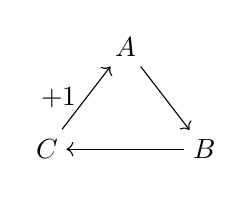
\begin{tikzpicture}[baseline=(current bounding box.center)]
      \node (A) at (1,1.3) {$A$}; \node (C) at (0,0)
      {$C$}; \node (B) at (2,0)
      {$B$}; \draw[->] (A) -- (B); \draw[->] (B) -- (C); \draw[->] (C)
      -- (A) node[midway, left] {$+1$};
    \end{tikzpicture}
  \]
  is a distinguished triangle in $\categ{K}(\categ{A})$ or
  $\categ{D}(\categ{A})$, then $\chi(B) = \chi(A) + \chi(C)$.
\end{exer}

\begin{exer}{\exerused{}}{exer:homol:9.2}
  Let $\categ{A}$ be an abelian category, and suppose two complexes
  $L^\bullet$, $M^\bullet$ are connected by an `upside-down roof' (a
  `trough'?)
  \[\begin{tikzcd}
      L^\bullet \arrow[dr] & & M^\bullet \arrow[dl,"\text{quasi-isomorphism}"] \\
      & N^\bullet &
    \end{tikzcd}\] Prove that they are also connected by a regular
  roof: there exists a complex $N^\bullet$ and morphisms
  $N^\bullet \to L^\bullet$ and $N^\bullet \to M^\bullet$ such that
  the diagram
  \[\begin{tikzcd}
      & N^\bullet \arrow[dl,"\text{quasi-isomorphism}"'] \arrow[dr] & \\
      L^\bullet \arrow[dr] & & M^\bullet \arrow[dl,"\text{quasi-isomorphism}"] \\
      & \underline{N}^\bullet &
    \end{tikzcd}\] commutes in $\categ{K}(\categ{A})$. Deduce that the
  composition of two roofs may be consolidated into a single roof in
  $\categ{K}(\categ{A})$. (Hint: Let
  $\alpha^\bullet : L^\bullet \to \underline{N}^\bullet$,
  $\beta^\bullet : M^\bullet \to \underline{N}^\bullet$ be the given
  morphisms, with $\beta^\bullet$ a quasi-isomorphism. Consider the
  composition
  $\gamma^\bullet : L^\bullet \to \underline{N}^\bullet \to
  MC(\beta)^\bullet$, and let $N^\bullet :=
  MC(\gamma)[-1]^\bullet$. We have
  $N^i = L^i \oplus M^i \oplus \underline{N}^{i-1}$, with morphisms to
  $L^i$, $M^i$ given, respectively, by $(\ell,m,n) \mapsto \ell$,
  $(\ell,m,n) \mapsto -m$; these define morphisms of cochain
  complexes. The morphisms $N^i \to \underline{N}^{i-1}$ defined by
  $(\ell,m,n) \mapsto -n$ define the homotopy showing that the diagram
  commutes in $\categ{K}(\categ{A})$. To verify that
  $N^\bullet \to L^\bullet$ is a quasi-isomorphism, use the fact that
  $MC(\beta)^\bullet$ is exact, and rotate a triangle.) [\S{}\ref{subsec:homol:derived-categories}]
\end{exer}

\begin{exer}{\exerused{}}{exer:homol:9.3}
  Let $\alpha^\bullet : L^\bullet \to M^\bullet$ be an isomorphism of
  cochain complexes. Prove that $MC(\alpha)^\bullet$ is homotopy
  equivalent to $0$. [\S{}\ref{subsec:homol:triangulated-categories}, \ref{exer:homol:9.4}]
\end{exer}

\begin{exer}{\exerused{}}{exer:homol:9.4}
  Let $\alpha^\bullet : L^\bullet \to M^\bullet$ be a cochain
  morphism, and let $\beta^\bullet : M^\bullet \to MC(\alpha)^\bullet$
  be the natural morphism. Prove that $MC(\beta)^\bullet$ is homotopy
  equivalent to $L[1]^\bullet$. (Hint: Do
  Exercise~\ref{exer:homol:9.3} first.) [\S{}\ref{subsec:homol:triangulated-categories}]
\end{exer}

\begin{exer}{\exerused{}}{exer:homol:9.5}
  Let
  \[
    0 \longrightarrow L^\bullet \xrightarrow{\alpha^\bullet} M^\bullet
    \xrightarrow{\beta^\bullet} N^\bullet \longrightarrow 0
  \]
  be a short exact sequence of cochain complexes on an abelian
  category.
  \begin{itemize}
  \item Prove that there is a cochain morphism
    $\gamma^\bullet : MC(\alpha)^\bullet \to N^\bullet$ through which
    $\beta^\bullet : M^\bullet \to N^\bullet$ factors.
  \item Prove that $MC(\gamma)^\bullet$ is an exact complex. (Hint:
    Chase elements.)
  \item Conclude that $MC(\alpha)^\bullet$ is quasi-isomorphic to
    $N^\bullet$.
  \end{itemize} [\S{}\ref{subsec:homol:triangulated-categories}]
\end{exer}

\begin{exer}{\exerused{}}{exer:homol:9.6}
  Let
  \[
    0 \longrightarrow L^\bullet \xrightarrow{\alpha^\bullet} M^\bullet
    \xrightarrow{\beta^\bullet} N^\bullet \longrightarrow 0
  \]
  be a short exact sequence of cochain complexes on an abelian
  category $\categ{A}$. Prove that there is a morphism
  $N^\bullet \to L[1]^\bullet$ in the derived category
  $\categ{D}(\categ{A})$, inducing the connecting morphism
  $H^i(N^\bullet) \to H^{i+1}(L^\bullet)$ in cohomology. [\S{}\ref{subsec:homol:triangulated-categories}]
\end{exer}

\begin{exer}{\exerused{}}{exer:homol:9.7}
  Prove Claim~\ref{fact:homol:9.1}. [\S{}\ref{subsec:homol:spectral-sequences}]
\end{exer}

\begin{exer}{\exerused{}}{exer:homol:9.8}
  Let $(E_r,d_r)_{r=1,2,\dots}$ be a spectral sequence arising from an
  exact couple
  \[
    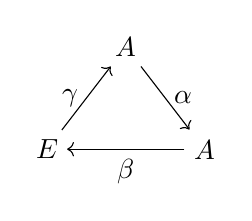
\begin{tikzpicture}[baseline=(current bounding box.center)]
      \node (A) at (1,1.3) {$A$}; \node (E) at (0,0)
      {$E$}; \node (A2) at (2,0)
      {$A$}; \draw[->] (A) -- (A2) node[midway, right]
      {$\alpha$}; \draw[->] (A2) -- (E) node[midway, below]
      {$\beta$}; \draw[->] (E) -- (A) node[midway, left] {$\gamma$};
    \end{tikzpicture}
  \]
  Prove that the limit $E_\infty$ is isomorphic to
  $\gamma^{-1}(\bigcap_r \image\alpha^r) / \beta(\bigcup_r
  \ker\alpha^r)$. (Hint: In fact,
  $Z_{r+1} = \gamma^{-1}(\image\alpha^r)$ and
  $B_{r+1} = \beta(\ker\alpha^r)$.) [\S{}\ref{subsec:homol:spectral-sequences}]
\end{exer}

\begin{exer}{}{exer:homol:9.9}
  Let ${}_vE_r$ be the spectral sequence of a first-quadrant double
  complex from the vertical filtration, as in \S{}9.3. Prove that
  ${}_vE_r^{i,j} = {}_vE_\infty^{i,j}$ for $r > j+1$.
\end{exer}

\begin{exer}{\exerused{}}{exer:homol:9.10}
  Let $\categ{A}$, $\categ{B}$, $\categ{C}$ be abelian categories, and
  let $\mathscr{F} : \categ{A} \to \categ{B}$,
  $\mathscr{G} : \categ{B} \to \categ{C}$ be additive functors. Assume
  that $\categ{A}$ and $\categ{B}$ have enough projectives, that
  $\mathscr{F}$ sends projectives of $\categ{A}$ to
  $\mathscr{G}$-acyclic objects of $\categ{B}$, and that $\mathscr{G}$
  is right-exact.

  Let $A$ be an object of $\categ{A}$, and let
  $M^\bullet : \dots \to M^{-2} \to M^{-1} \to M^0 \to 0$ be a
  projective resolution of $A$. Let $P_{\mathscr{F}M^\bullet}^\bullet$
  be a Cartan--Eilenberg resolution of the complex
  $\mathscr{F}M^\bullet$ (as constructed in \Cref{coro:homol:7.9}). Consider
  the complex
  \[
    (\dagger) \qquad \dots \longrightarrow
    \mathscr{G}(P_{\mathscr{F}M^{-2}}^\bullet) \longrightarrow
    \mathscr{G}(P_{\mathscr{F}M^{-1}}^\bullet) \longrightarrow
    \mathscr{G}(P_{\mathscr{F}M^0}^\bullet) \longrightarrow 0
  \]
  obtained by applying $\mathscr{G}$ to
  $P_{\mathscr{F}M^\bullet}^\bullet$.

  This is precisely the set-up of \Cref{exer:homol:8.8}. Now take the double
  complex associated with $(\dagger)$, and construct the spectral
  sequence corresponding to the horizontal filtration. Prove that the
  $E_2$ term of this sequence has terms
  \[ {}_hE_2^{p,q} =
    \categ{L}_p\mathscr{G}(\categ{L}_q\mathscr{F}(A)).
  \]
  (Use \Cref{exer:homol:7.6} to compute the ${}_hE_1$ term.)

  This is the Grothendieck spectral sequence mentioned at the end of
  \S{}9.3. Prove that it abuts to
  $\categ{L}_\bullet(\mathscr{G} \circ \mathscr{F})(A)$.

  (Use the `horizontal' version of Theorem~\ref{homol:9.5}, together
  with the computation of the cohomology of the total complex from
  \Cref{exer:homol:8.8}.) [\S{}\ref{subsec:homol:universal-property-of-the-derived-functor}, \ref{exer:homol:7.6}, \S{}\ref{subsec:homol:spectral-sequences}]
\end{exer}

%%% Local Variables:
%%% mode: LaTeX
%%% TeX-engine: luatex
%%% TeX-master: "../master"
%%% End:


\backmatter{}
\nocite{*}
\chapter*{Bibliography}
\printbibliography{}
\printindex{}


\end{document}

%%% Local Variables:
%%% mode: latex
%%% TeX-engine: luatex
%%% TeX-master: t
%%% End:
